Evaluating the performance of the hybrid automaton primarily involves the
evaluation of the steady-state errors regarding the position and angle of the
robot with regard to the selected goal position. In order to obtain a broader
understanging of how the four $K_{*}$ gains influence the trajectory of the
robot, twelve combinations were considered for the 4-tuple
$$(K_{\Psi}^R, K_{\omega}^R, K_{\Psi}^T, K_{\omega}^T)$$
where
$$K_{\Psi}^R \in \{0.1,0.2,0.5\} \cdot K_{\Psi,max}^R$$
$$K_{\omega}^T \in \{0.1,0.2,0.5,0.75\} \cdot K_{\omega,max}^T$$
$$K_{\omega}^R = 0.5 K_{\omega,max}^R \text{, and } K_{\Psi}^T = 0.5 K_{\Psi,max}^T$$


Figures \ref{fig:19_1_distance} - \ref{fig:19_12_distance} on the left-hand side
illustrate the evolution of the distance of the robot in relation to its goal,
while figures on the right-hand side display the evolution of the angular
error over time. The goal was set to be node 1 $N1(-0.37, 1.68)$, and the
robot's initial pose was $(x_0, y_0, \theta_0) \equiv (0,0,0)$. Hence, the
distance to the goal was $d_g = 1.7203$ meters and the angle to the goal
$\theta^R = 102.42^{\circ}$. The distance and angle tolerance thresholds where
taken to be $d_{th} = 2\text{ cm}$ and $\theta_{th} = 2^{\circ}$ respectively.

Since the actual final pose is not defined deterministically, five simulations
of each possible combination of settings for the aforementioned 4-tuple were
conducted.  Hence, all the following figures express the mean steady-state
positional and angular errors across five runs.

Table \ref{tbl:19_errors} illustrates the steady-state errors $e_d$ and
$e_{\theta}$ regarding the distance and the angle that the robot had to travel,
respectively.

\noindent\makebox[\textwidth][c]{%
\begin{minipage}{\linewidth}
  \begin{minipage}{0.45\linewidth}
    \begin{figure}[H]
      \scalebox{0.6}{% This file was created by matlab2tikz.
%
%The latest updates can be retrieved from
%  http://www.mathworks.com/matlabcentral/fileexchange/22022-matlab2tikz-matlab2tikz
%where you can also make suggestions and rate matlab2tikz.
%
\definecolor{mycolor1}{rgb}{0.00000,0.44700,0.74100}%
%
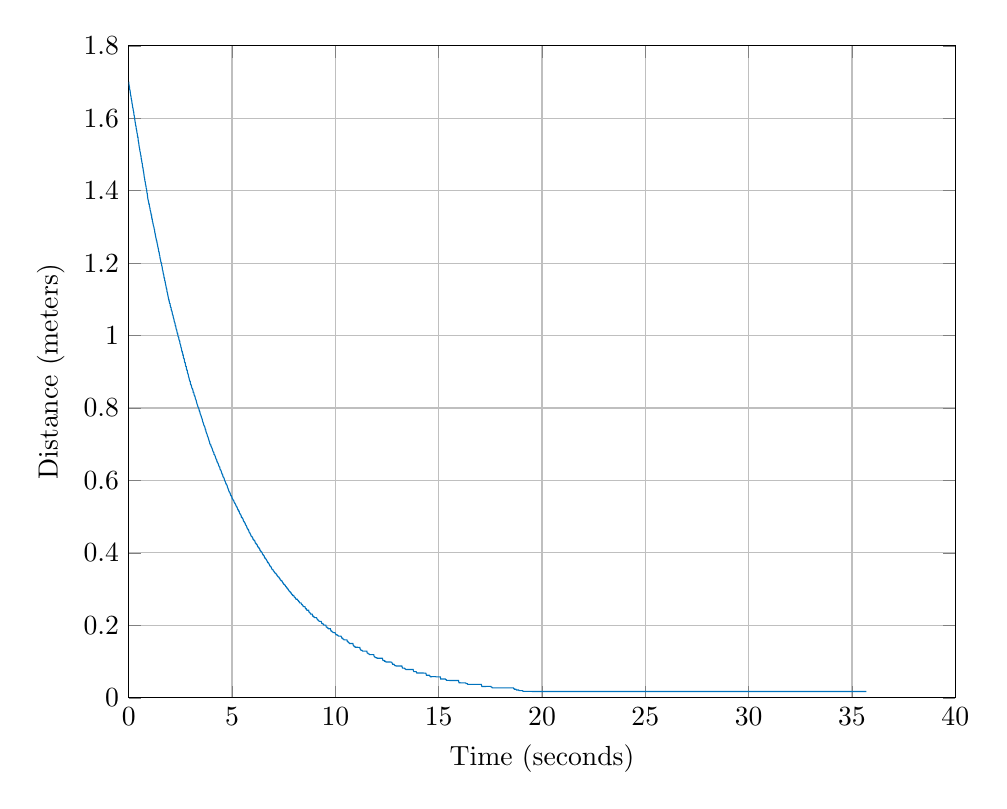
\begin{tikzpicture}

\begin{axis}[%
width=4.133in,
height=3.26in,
at={(0.693in,0.44in)},
scale only axis,
xmin=0,
xmax=40,
xmajorgrids,
xlabel={Time (seconds)},
ymin=0,
ymax=1.8,
ymajorgrids,
ylabel={Distance (meters)},
axis background/.style={fill=white}
]
\addplot [color=mycolor1,solid,forget plot]
  table[row sep=crcr]{%
0	1.70068123431103\\
0.0160897579999976	1.69088964753209\\
0.0319536779999994	1.68892882967893\\
0.0479920889999978	1.67911944683444\\
0.0639707249999978	1.67715733339095\\
0.0798784100000001	1.66931006398995\\
0.0956978090000004	1.66342415149956\\
0.111957416999999	1.65950068114547\\
0.128051428999998	1.65165211615414\\
0.14399943	1.64969129830098\\
0.160010939999998	1.64106031941871\\
0.175838598999999	1.63793889366888\\
0.191816116999999	1.63009032867755\\
0.207814406999998	1.6281295108244\\
0.223821577	1.62028094583307\\
0.239795623	1.61832012797991\\
0.255993369999997	1.60851074513542\\
0.272041316999998	1.60654863169193\\
0.288001781999998	1.59870136229094\\
0.303989943999998	1.592420477305\\
0.320019404999997	1.58694895765884\\
0.335718961999997	1.58106304516844\\
0.353927765999999	1.57713957481435\\
0.369079860999998	1.56929100982302\\
0.384440294	1.56733019196986\\
0.399938083000001	1.55948162697854\\
0.416010779999997	1.55752080912538\\
0.432001287	1.54771142628089\\
0.448041647999998	1.54771142628089\\
0.464019436000001	1.53672568367769\\
0.479964224999998	1.5339969082053\\
0.495825263999999	1.5261496388043\\
0.511809708000001	1.52026372631391\\
0.527817193999998	1.51634025595982\\
0.543979698999997	1.50849169096849\\
0.560019064999998	1.50653087311533\\
0.575987351	1.498682308124\\
0.591711323999997	1.49672149027084\\
0.607884502	1.4876965655208\\
0.623764432999998	1.48496908563874\\
0.639765484999999	1.47712052064742\\
0.655662213999998	1.47515970279426\\
0.671636743000001	1.46535031994977\\
0.689965912	1.46338820650628\\
0.705555713999998	1.45554093710529\\
0.720974097999997	1.4516156359297\\
0.736425042999998	1.4457315542608\\
0.752013825999998	1.43748801677392\\
0.767985169999998	1.4347458116576\\
0.784064397999998	1.42613058463737\\
0.799987377999999	1.42416976678421\\
0.815949996999998	1.41632120179289\\
0.831790041999999	1.41436038393973\\
0.847703535	1.4065118189484\\
0.865792719	1.40455100109524\\
0.881333802999999	1.39474161825075\\
0.896977730999999	1.39238453231171\\
0.912544237	1.38375587564755\\
0.928034802999999	1.37710330112826\\
0.945558377999999	1.37317983077417\\
0.961012855999999	1.36925452959859\\
0.976674483999997	1.36337044792968\\
0.992287300999999	1.36337044792968\\
1.008084606	1.35552188293835\\
1.024006267	1.35356106508519\\
1.039927593	1.34571250009387\\
1.055869966	1.34375168224071\\
1.071930402	1.33943140856958\\
1.087707123	1.33276593963751\\
1.105888396	1.33276593963751\\
1.120954996	1.32218989476412\\
1.136063254	1.32218989476412\\
1.151965903	1.31434132977279\\
1.167860859	1.31238051191964\\
1.183883855	1.30649459942924\\
1.199989118	1.30257112907515\\
1.215862459	1.30060901563166\\
1.232039114	1.29472256408382\\
1.248006594	1.29236677373511\\
1.263905499	1.28412426287602\\
1.280009479	1.28177600362746\\
1.295979119	1.27550538974564\\
1.312351161	1.27119995875408\\
1.329028631	1.26727465757849\\
1.345439439	1.26139057590959\\
1.360552409	1.26139057590959\\
1.375791279	1.25354201091826\\
1.391800864	1.2515811930651\\
1.408044063	1.24569528057471\\
1.424009134	1.24177181022062\\
1.439880985	1.23745153654949\\
1.455897499	1.23117350901281\\
1.471946133	1.23078606761741\\
1.487924228	1.22255280123466\\
1.503861733	1.22021002274403\\
1.519953392	1.2123614577527\\
1.535875289	1.21040063989954\\
1.551796555	1.20451472740915\\
1.567954402	1.20059125705506\\
1.585072609	1.20059125705506\\
1.6001091	1.19274269206373\\
1.615910449	1.19038690171502\\
1.631744493	1.18214439085593\\
1.650183271	1.17979613160737\\
1.665421329	1.17391021911698\\
1.680748253	1.16922008673398\\
1.696036406	1.16725797329049\\
1.712164869	1.1594107038895\\
1.728029274	1.1594107038895\\
1.743724123	1.15156213889817\\
1.761874765	1.14960132104501\\
1.775701723	1.14371540855462\\
1.791698329	1.13979193820053\\
1.807879386	1.1354716645294\\
1.823789066	1.12919363699272\\
1.839707785	1.12880619559732\\
1.855712836	1.120957630606\\
1.873810618	1.11823015072394\\
1.889502569	1.11234423823355\\
1.90466208	1.10842076787945\\
1.919976525	1.10449546670387\\
1.935864982	1.09861138503497\\
1.953506925	1.09861138503497\\
1.968487134	1.0907628434884\\
1.983818934	1.08880216486104\\
1.999818998	1.08840719236549\\
2.015802681	1.08016497707164\\
2.031806483	1.07820444108262\\
2.047818294	1.07781631480404\\
2.063814584	1.06996831779739\\
2.079930571	1.06762199929571\\
2.095697073	1.06723886477308\\
2.113944877	1.05939079788469\\
2.128990905	1.05742993765509\\
2.144018206	1.05546802049092\\
2.159971493	1.04958206911173\\
2.176284206	1.04762125125857\\
2.19193897	1.04369664932629\\
2.207897159	1.03781293919267\\
2.224002575	1.03741796669712\\
2.239971831	1.03349364332665\\
2.255735934	1.02721612600849\\
2.271913257	1.02721612600849\\
2.288129203	1.02094163196418\\
2.303891374	1.01701863307614\\
2.319898861	1.01663171175507\\
2.335729801	1.0103619490539\\
2.351904852	1.00643901775724\\
2.367892147	1.00643892428117\\
2.3839647	0.998592087872643\\
2.399926091	0.996631278987214\\
2.415853571	0.996631257092948\\
2.431898297	0.98878469629541\\
2.447740279	0.986823959529769\\
2.463828242	0.986429036841328\\
2.479907672	0.978188806085808\\
2.495841785	0.976228141559486\\
2.511868449	0.973875689527261\\
2.527856471	0.967990784451318\\
2.543846042	0.965641301242969\\
2.559754994	0.961331467105665\\
2.577828309	0.955448195457458\\
2.592816777	0.955448144263153\\
2.607849516	0.951524589525238\\
2.623834295	0.945641385767252\\
2.639808475	0.945641480270402\\
2.655837666	0.93779575285993\\
2.671814678	0.935834997875439\\
2.687989072	0.935440265819491\\
2.70402198	0.927200796570331\\
2.719988293	0.925240113956512\\
2.735943856	0.924847407487987\\
2.752031729	0.91700226226651\\
2.76788889	0.9150416521429\\
2.783834736	0.914651415351239\\
2.800009561	0.906418421290018\\
2.81591439	0.904457541340465\\
2.831949859	0.904457541340465\\
2.847911837	0.896612626218602\\
2.863985212	0.894651819010136\\
2.880055094	0.892690932430317\\
2.895895216	0.886807255550577\\
2.911863428	0.88445146520187\\
2.927844866	0.88052888837378\\
2.945223863	0.87621319892731\\
2.960330328	0.874252381074151\\
2.975859034	0.873858092985109\\
2.991861199	0.86601352412947\\
3.007819368	0.864052706276311\\
3.023806337	0.863661498609867\\
3.039863035	0.859738907062859\\
3.055853993	0.855428118639761\\
3.071848956	0.853467300786602\\
3.087712025	0.853467300786602\\
3.10594866	0.849544709239594\\
3.121195041	0.843661914077805\\
3.136474965	0.843661914077805\\
3.151898082	0.841701165011035\\
3.167987388	0.835817345222166\\
3.18398093699999	0.833856527369007\\
3.199899092	0.833461554873459\\
3.215971575	0.829145017458682\\
3.232019748	0.825223040150052\\
3.248014114	0.823262222296893\\
3.265369539	0.820906091727612\\
3.280866613	0.816984731346032\\
3.29628096	0.813062547499052\\
3.312035143	0.810320686237903\\
3.327938353	0.808359937171133\\
3.34377397	0.804437959862503\\
3.359933244	0.802477142009344\\
3.375866061	0.800515299529105\\
3.391843524	0.798554550462335\\
3.407851421	0.794632573153705\\
3.423738369	0.790709912820308\\
3.439848016	0.790709912820308\\
3.455863976	0.784827186444907\\
3.471854112	0.7824713960962\\
3.487983375	0.780509553615962\\
3.504005976	0.778154858681423\\
3.519959344	0.774232881372793\\
3.535985562	0.772272063519634\\
3.551910997	0.769915932950353\\
3.567961576	0.765994572568773\\
3.583852823	0.762072388721794\\
3.600895274	0.759719338575111\\
3.616043615	0.757369778393874\\
3.63191856	0.753447801085244\\
3.647988928	0.751486983232085\\
3.663720047	0.749525140751847\\
3.681864472	0.747564391685077\\
3.697335704	0.743642414376446\\
3.712475215	0.739719754043049\\
3.728121718	0.739719754043049\\
3.743769059	0.733837027667649\\
3.759808097	0.731481237318942\\
3.775863435	0.729519394838704\\
3.791875624	0.727164699904165\\
3.807877261	0.723242722595534\\
3.825246817	0.721281904742375\\
3.840286841	0.718925774173094\\
3.855819727	0.716965025106324\\
3.872014136	0.713043047797694\\
3.887923971	0.709120387464297\\
3.906402104	0.708340368683386\\
3.92154449	0.702457642307985\\
3.936800611	0.700496824454826\\
3.951952278	0.698534981974588\\
3.968264268	0.698535034827028\\
3.984004137	0.694613777624467\\
4.00002793	0.692652411630647\\
4.015872097	0.690691790654598\\
4.031817083	0.688730057446926\\
4.047768571	0.686769308380156\\
4.063906237	0.682847469062381\\
4.07991689	0.680491177726255\\
4.095797978	0.678529335246017\\
4.111834936	0.678134362750469\\
4.127813045	0.672251628825828\\
4.143808018	0.672251628825828\\
4.160119192	0.670291086476585\\
4.175796888	0.667934823056173\\
4.191878565	0.665974073989403\\
4.207833272	0.662052442105799\\
4.223784415	0.660091987630945\\
4.239900495	0.657738936941601\\
4.255930739	0.657350125827134\\
4.271798102	0.651467908777799\\
4.287772292	0.651467914699059\\
4.303726774	0.649507579604835\\
4.319767131	0.647545838285111\\
4.335687433	0.645585170807962\\
4.353794113	0.641663746895948\\
4.36873338199999	0.639703658133584\\
4.383731918	0.637741973030753\\
4.401829355	0.637741973030753\\
4.416871809	0.63185986949525\\
4.431886912	0.629501765563451\\
4.447840495	0.629501765563451\\
4.464240019	0.627539923083213\\
4.479766231	0.625181622097063\\
4.495725077	0.621260406694\\
4.51184098	0.619300348775807\\
4.527728724	0.616944186201903\\
4.543808267	0.616944186201903\\
4.559731013	0.611062291354459\\
4.575864124	0.609102373346475\\
4.591700156	0.609102423489716\\
4.609827652	0.606749373343034\\
4.62523766	0.604399890403285\\
4.639714331	0.600478940964284\\
4.65568819	0.598519091555042\\
4.671738838	0.596557402892324\\
4.687785006	0.59459678714031\\
4.703740409	0.590675850584979\\
4.719805106	0.590675850584979\\
4.735729865	0.588716511142159\\
4.751697172	0.586754668661921\\
4.767706208	0.584793919595151\\
4.783817213	0.580472788954432\\
4.79972791	0.578513148591445\\
4.815770482	0.576551306111207\\
4.83174113	0.574190718762607\\
4.84775243	0.570269991969848\\
4.865789421	0.568310421408337\\
4.880655858	0.568310498948424\\
4.89573418	0.565954368379144\\
4.911720235	0.563993619312374\\
4.927793645	0.560073088993568\\
4.945439288	0.558113693471374\\
4.960785798	0.558113693471374\\
4.975885795	0.555760643324692\\
4.991689987	0.553799894257922\\
5.009886759	0.549490496490841\\
5.023800516	0.549490496490841\\
5.03988035	0.547531065711356\\
5.055861068	0.545569223231118\\
5.071787135	0.545569223231118\\
5.087705756	0.543608474164348\\
5.10385642599999	0.539687887511733\\
5.119802903	0.537728456732248\\
5.135883138	0.537728456732248\\
5.15176973	0.53576661425201\\
5.167889179	0.53380586518524\\
5.183793306	0.531844499191419\\
5.199822591	0.529483464632724\\
5.215866711	0.527524033853239\\
5.231857859	0.527524033853239\\
5.247819747	0.525161403373671\\
5.263857587	0.523200654306901\\
5.28000055	0.519280067654286\\
5.29593066	0.519280067654286\\
5.311948861	0.517320636874801\\
5.327897358	0.51496450630552\\
5.343920795	0.51496450630552\\
5.359956064	0.51104239124493\\
5.375887048	0.509083170586136\\
5.391862114	0.507123739806651\\
5.407927441	0.507123739806651\\
5.423848111	0.504770689659968\\
5.439971504	0.502809940593199\\
5.455821816	0.498500542826117\\
5.47432783	0.498500542826117\\
5.489483882	0.496541112046632\\
5.50460508	0.496541112046632\\
5.519941561	0.494579269566394\\
5.53580394	0.492618520499624\\
5.551878507	0.488697933847009\\
5.567854877	0.486738503067524\\
5.583926944	0.486738503067524\\
5.599865344	0.484776660587286\\
5.616002659	0.482815911520516\\
5.631837098	0.482414097620615\\
5.647868072	0.478493510968\\
5.663892301	0.476534080188515\\
5.679878519	0.476133292189185\\
5.695886266	0.474171449708947\\
5.711980764	0.472210700642177\\
5.728302401	0.468290113989563\\
5.743884077	0.468290113989563\\
5.759937412	0.466330683210078\\
5.775891021	0.463974552640797\\
5.79188713199999	0.463974552640797\\
5.807848122	0.462013803574027\\
5.823883401	0.458093216921412\\
5.839745047	0.456133786141927\\
5.855713126	0.456133786141927\\
5.871829922	0.453780735995245\\
5.887911185	0.451819986928475\\
5.904018648	0.449858620934654\\
5.919849897	0.447510589161393\\
5.935959256	0.445551158381908\\
5.953422475	0.445551158381908\\
5.968718993	0.44358931590167\\
5.9840129	0.443589537291348\\
5.999898635	0.441628986315762\\
6.016275572	0.437708469822743\\
6.031868259	0.437708769197847\\
6.047752824	0.435749684296493\\
6.063896802	0.435749684296493\\
6.079925594	0.43378814901718\\
6.095740294	0.433788432740614\\
6.111896709	0.431424843983531\\
6.128028471	0.427504511448493\\
6.143813311	0.427504802997767\\
6.159945732	0.425143496656276\\
6.175912126	0.425143548013788\\
6.191939857	0.423181733197787\\
6.207944025	0.423181733197787\\
6.223947126	0.421221043386284\\
6.239808296	0.417300914148384\\
6.255847523	0.417300914148384\\
6.271875481	0.41534204181807\\
6.28784224	0.414947753729027\\
6.303714388	0.412986025047171\\
6.319710418	0.412986025047171\\
6.337904429	0.411025421608477\\
6.352959396	0.407105519659334\\
6.368142816	0.407105519659334\\
6.383905071	0.405146874617745\\
6.400866524	0.405147074788951\\
6.416284263	0.402794024642269\\
6.43187053	0.402794256881798\\
6.44772719799999	0.400833716003324\\
6.463856821	0.398872350009504\\
6.479726095	0.396525333530385\\
6.495976907	0.394566892024631\\
6.514377265	0.394566892024631\\
6.529615927	0.392605368633989\\
6.544798225	0.392605663493415\\
6.560048625	0.390644914426646\\
6.575737101	0.386725571669433\\
6.591978104	0.386725874605592\\
6.608053468	0.384767358228058\\
6.623943335	0.384767764406308\\
6.63996426	0.38280592192607\\
6.655944069	0.382399703720442\\
6.671816115	0.380438954653672\\
6.687787747	0.378477661204499\\
6.703896302	0.376519889110517\\
6.719942851	0.374155597907444\\
6.736043975	0.374155749655367\\
6.751954952	0.372194034297937\\
6.768010797	0.372194034297937\\
6.783993427	0.370233445187453\\
6.800028273	0.368272214524817\\
6.816005237	0.366314194694051\\
6.83185824	0.36435620103811\\
6.847723037	0.363962127483531\\
6.863904275	0.362000285003293\\
6.879986174	0.362000532609781\\
6.895900382	0.360040006345491\\
6.911902428	0.358078640351671\\
6.927939957	0.356121090095854\\
6.945522832	0.354163749316736\\
6.961017348	0.354163749316736\\
6.976162362	0.353772199333307\\
6.991806175	0.351810600730766\\
7.007799715	0.349850231022455\\
7.023806784	0.349850231022455\\
7.039722328	0.347889344195101\\
7.055830125	0.34593185276765\\
7.071805479	0.345542014488207\\
7.087886727	0.343584153953145\\
7.103890354	0.343584556664297\\
7.119727807	0.343584556664297\\
7.135781821	0.341623087896186\\
7.151825635	0.339663034058191\\
7.167809677	0.339663034058191\\
7.183802264	0.33770204070591\\
7.199845201	0.335744896654445\\
7.215949942	0.335744896654445\\
7.231977453	0.333787233289327\\
7.248047842	0.33337938066264\\
7.263994956	0.33337938066264\\
7.28002144	0.33141801466882\\
7.295854701	0.329458145116434\\
7.311836183	0.329458648657795\\
7.327999453	0.327087813689531\\
7.343720657	0.325130383587797\\
7.359750997	0.325130737691424\\
7.375744488	0.323173288921319\\
7.391757902	0.323173681963862\\
7.407743476	0.323174124684738\\
7.423753102	0.321212963795624\\
7.440009378	0.319253384421664\\
7.45603924	0.317293232853666\\
7.472045303	0.317293232853666\\
7.48799013199999	0.315335426723373\\
7.503984754	0.313379303884435\\
7.519842674	0.31298125215638\\
7.535808798	0.31298125215638\\
7.551825675	0.311021171681499\\
7.567831126	0.311021171681499\\
7.58391047	0.30906125270957\\
7.599843631	0.307101539344777\\
7.615828933	0.307101895762836\\
7.631820564	0.305144089632543\\
7.64803739	0.303187785563804\\
7.663970657	0.303188222509418\\
7.679969338	0.302791881345321\\
7.695950163	0.300831562301657\\
7.712022932	0.298872337362349\\
7.72783467	0.298872337362349\\
7.743811652	0.296912657348474\\
7.759780831	0.294955422924371\\
7.775815899	0.294560792626065\\
7.791830281	0.292604179795743\\
7.807810259	0.292604840966074\\
7.823820316	0.292604840966074\\
7.839921467	0.290644229651264\\
7.855745344	0.288685754941981\\
7.871937664	0.288685754941981\\
7.887972226	0.286725697023788\\
7.903988954	0.284769091100571\\
7.919985109	0.284769091100571\\
7.936000358	0.282403783361417\\
7.953667013	0.282404165616218\\
7.969291525	0.282404165616218\\
7.984937587	0.282404165616218\\
8.000574449	0.280443999754698\\
8.016030496	0.278070683479175\\
8.031957755	0.278070683479175\\
8.047838489	0.276111081264974\\
8.063805799	0.276111390183075\\
8.079936113	0.274153584052781\\
8.095880115	0.272197182734551\\
8.111749332	0.272197500470196\\
8.127845991	0.272197500470196\\
8.143840954	0.272197500470196\\
8.159801403	0.272198091853619\\
8.175695111	0.270237964551853\\
8.193934604	0.268278533772368\\
8.209020487	0.268279212174477\\
8.224103343	0.266319641612966\\
8.239854649	0.266319641612966\\
8.255987203	0.264362601440752\\
8.27200196	0.262005156110546\\
8.287991902	0.262005156110546\\
8.304103444	0.262005939823096\\
8.319973879	0.262005939823096\\
8.335811619	0.262005939823096\\
8.35187193	0.260046460077088\\
8.36784308	0.258087461101366\\
8.383859346	0.258087461101366\\
8.399832785	0.256128548465302\\
8.416145602	0.256129059186463\\
8.432007984	0.254171253056169\\
8.447997249	0.252215052825111\\
8.463962927	0.25221557248311\\
8.479981321	0.251813758583209\\
8.49598574	0.251813758583209\\
8.511996037	0.251814411272383\\
8.528015631	0.251814411272383\\
8.543988584	0.247895340129911\\
8.559994626	0.245937000226607\\
8.57602927899999	0.245937000226607\\
8.59186519099999	0.245937000226607\\
8.608018402	0.243980022697526\\
8.623752027	0.241622919358609\\
8.639900513	0.241622919358609\\
8.655846044	0.241623423973826\\
8.671819578	0.241623423973826\\
8.687806558	0.241623423973826\\
8.703957699	0.241623653759599\\
8.71999195	0.237705155028093\\
8.735963265	0.235746285764047\\
8.751981199	0.235746594598809\\
8.767923763	0.23533831650412\\
8.783728265	0.233380510373827\\
8.799749609	0.231423853042952\\
8.815735969	0.231424552328099\\
8.831766065	0.231424552328099\\
8.847721656	0.231010436294201\\
8.863711797	0.231011153716122\\
8.881796925	0.231011153716122\\
8.89680264	0.227092572437438\\
8.911742919	0.225134791141221\\
8.929771954	0.225134791141221\\
8.944795547	0.225134791141221\\
8.96002886	0.22317740039832\\
8.975705053	0.22317740039832\\
8.991703502	0.221220743067445\\
9.007691827	0.221221167582906\\
9.023741247	0.221221167582906\\
9.039814408	0.221221167582906\\
9.055698037	0.221221601226423\\
9.071878043	0.221221601226423\\
9.087711782	0.221221601226423\\
9.103753384	0.219262613218498\\
9.119766646	0.217303814412422\\
9.135703551	0.215345227338257\\
9.1537201	0.215345227338257\\
9.168616853	0.215345749755484\\
9.183711207	0.212987155625861\\
9.199709602	0.212987155625861\\
9.21779804399999	0.211031029899894\\
9.232689685	0.211031029899894\\
9.247699725	0.211031029899894\\
9.265817141	0.211031570692468\\
9.28083964	0.211031570692468\\
9.295762912	0.211031570692468\\
9.313799604	0.211032120672691\\
9.328604545	0.207114173515672\\
9.343755081	0.205155586441507\\
9.359728792	0.205156216365653\\
9.375702028	0.205156216365653\\
9.391726733	0.205156216365653\\
9.40771678	0.203199049406778\\
9.423709983	0.202794158467246\\
9.441851223	0.200837501136371\\
9.456803903	0.200837501136371\\
9.471770587	0.200838149555043\\
9.487708791	0.200838149555043\\
9.503716851	0.200838807220948\\
9.519732638	0.200838807220948\\
9.537791066	0.200838807220948\\
9.552835377	0.196921143447029\\
9.568047544	0.194963294280892\\
9.583708081	0.194963294280892\\
9.601805435	0.194963294280892\\
9.616733031	0.192598951863188\\
9.631751434	0.192598951863188\\
9.647858462	0.192598951863188\\
9.66375912	0.190642709308866\\
9.681867938	0.190642709308866\\
9.696752042	0.190642709308866\\
9.711716434	0.190643133404633\\
9.728441978	0.190643133404633\\
9.743786498	0.190643133404633\\
9.759705931	0.190643566819601\\
9.775751958	0.186726258616691\\
9.791720329	0.184359021134248\\
9.807716831	0.184359535161535\\
9.823737307	0.184359535161535\\
9.839703534	0.182401729031241\\
9.855713313	0.181987612997343\\
9.871694791	0.181988136403442\\
9.889764468	0.180031479072567\\
9.904783004	0.180031479072567\\
9.919835799	0.180031479072567\\
9.935731696	0.180031479072567\\
9.953105679	0.180032118732444\\
9.969136166	0.180032118732444\\
9.984637749	0.180032300443137\\
9.999805784	0.178073326753486\\
10.015884821	0.176115933337\\
10.031943927	0.174157537364784\\
10.047842662	0.174157933912836\\
10.063734863	0.17415828466499\\
10.079886564	0.174158485158188\\
10.095827008	0.172201299251914\\
10.111840862	0.172201659395175\\
10.127876337	0.172201940811286\\
10.143811474	0.170245988490288\\
10.159722677	0.170246430569718\\
10.177800924	0.170246721436696\\
10.192630798	0.170246721436696\\
10.207733095	0.170247597831074\\
10.223735017	0.170247898148908\\
10.239677655	0.170247898148908\\
10.257796282	0.170248793432663\\
10.272687811	0.170248793432663\\
10.287668127	0.168290163538999\\
10.305706831	0.166333413332879\\
10.320664837	0.164374826258714\\
10.335724801	0.164375145478235\\
10.351720232	0.164375669116579\\
10.36976637	0.162015049989899\\
10.384655237	0.162015450490045\\
10.399702898	0.162015641757999\\
10.415738026	0.160060199508413\\
10.431709129	0.160060609518997\\
10.447718963	0.160060810297589\\
10.46582114	0.160061381983458\\
10.481384466	0.160061801504467\\
10.496391821	0.160061801504467\\
10.511756633	0.160062592989729\\
10.527731554	0.160063022021149\\
10.54372827	0.160063022021149\\
10.559828142	0.160063832527188\\
10.575713204	0.156147581372131\\
10.593820057	0.15614801991395\\
10.609219623	0.154190333122866\\
10.62418276	0.154190333122866\\
10.639718532	0.152233979409639\\
10.657818029	0.151830007833573\\
10.672834599	0.151830007833573\\
10.687741497	0.149874971110108\\
10.705830963	0.1498752903174\\
10.720842781	0.149875982754397\\
10.736189632	0.149876522074412\\
10.751702897	0.149876850851955\\
10.769829006	0.149877552858596\\
10.784782338	0.149878101748558\\
10.799717251	0.149878440096342\\
10.817776296	0.149879151672606\\
10.832788532	0.149879710132499\\
10.847788781	0.149879710132499\\
10.863787416	0.145964953473886\\
10.87999554	0.144006366399721\\
10.895847871	0.143597942325844\\
10.912305332	0.141642661411704\\
10.927920529	0.141642661411704\\
10.945410549	0.141643311496886\\
10.960781698	0.139688925404641\\
10.976383135	0.139688925404641\\
10.991846102	0.139689585119296\\
11.007993876	0.139689585119296\\
11.023916083	0.139690408531672\\
11.039890274	0.139691077875779\\
11.055929968	0.139691077875779\\
11.071980848	0.139691910917221\\
11.087837015	0.139276083658624\\
11.103926457	0.139276083658624\\
11.120013246	0.139276926329106\\
11.136058875	0.139277273525833\\
11.151917681	0.139277273525833\\
11.167940228	0.138855476232419\\
11.183863885	0.138855833071234\\
11.1998458	0.134940078462946\\
11.215981957	0.132982012141196\\
11.231826586	0.132982012141196\\
11.248099656	0.131026447039833\\
11.264348123	0.131026977434096\\
11.279806284	0.131026977434096\\
11.295926711	0.131027426459649\\
11.314327649	0.129073356273935\\
11.329612798	0.129073356273935\\
11.344864778	0.129073815001122\\
11.360165914	0.129073815001122\\
11.375749477	0.129074438653705\\
11.391934729	0.129074907082512\\
11.408002647	0.129074907082512\\
11.423916117	0.129075540436431\\
11.43989936	0.129076018566844\\
11.455977418	0.129076018566844\\
11.471881011	0.129076661622081\\
11.48788389	0.129077149454084\\
11.503904392	0.129077149454084\\
11.519925852	0.12907780221062\\
11.535936278	0.125162047602331\\
11.551887481	0.123203958061746\\
11.567930748	0.12320462051956\\
11.583780383	0.12320462051956\\
11.599926492	0.121249707741684\\
11.616311273	0.121250379900755\\
11.631761165	0.121250379900755\\
11.650138038	0.119296804676301\\
11.665383554	0.11929756086848\\
11.680513011	0.11929756086848\\
11.6958424	0.119298160885859\\
11.711833059	0.119298160885859\\
11.727856841	0.119298926838781\\
11.74388585	0.119299536617234\\
11.759785888	0.119299536617234\\
11.775896503	0.119300312330874\\
11.794647625	0.119300931870384\\
11.809744182	0.119300931870384\\
11.825813772	0.119301717344719\\
11.840910214	0.119302346645266\\
11.856001712	0.119302346645266\\
11.871766501	0.115387387271983\\
11.887786144	0.113428800197818\\
11.903873333	0.113021814011968\\
11.919940088	0.11302330999641\\
11.935879975	0.111068330794397\\
11.953400802	0.111068640815517\\
11.968470278	0.111070729652272\\
11.983956461	0.111070729652272\\
11.999922284	0.111071049494588\\
12.016035113	0.109118699284947\\
12.032097839	0.109119598550317\\
12.047938366	0.109119928213819\\
12.063992629	0.109121241529426\\
12.07982449	0.109122150614877\\
12.095798191	0.109122490099555\\
12.111806218	0.109123092809261\\
12.127697026	0.109124741938169\\
12.143887722	0.109124741938169\\
12.159703668	0.109125703762584\\
12.175918559	0.109127372520117\\
12.191731609	0.109127372520117\\
12.207788042	0.109127731647114\\
12.223729141	0.109130042360638\\
12.241961147	0.109130042360638\\
12.257405001	0.109130411308779\\
12.272600979	0.109132751459651\\
12.287736111	0.107175231098245\\
12.303923903	0.1032604287052\\
12.319879667	0.102854357864116\\
12.335827307	0.102855316049553\\
12.351850138	0.102855776290877\\
12.367806803	0.102857008701046\\
12.383736779	0.10090299750438\\
12.39989411	0.100903467626438\\
12.415955733	0.100904719785542\\
12.431817408	0.100905697610771\\
12.447818669	0.0989532085844598\\
12.463901798	0.0989536095410937\\
12.47971686	0.098955543421539\\
12.495742671	0.098955543421539\\
12.511817457	0.0989560333050223\\
12.527768857	0.0989583977702699\\
12.54373972	0.0989583977702699\\
12.55968015	0.0989588975344435\\
12.575729069	0.0989612916277873\\
12.591816674	0.0989612916277873\\
12.607899184	0.0989618012726363\\
12.623863211	0.0989631324270934\\
12.639888843	0.0989642249940028\\
12.655912932	0.0989647445195114\\
12.690501026	0.0985527403401114\\
12.706252925	0.0985527403401114\\
12.722229719	0.0985532697462637\\
12.738284196	0.0965985373479619\\
12.754285939	0.0946420246900554\\
12.77031624	0.0926851873345977\\
12.786326511	0.0926875025468419\\
12.802438358	0.0926875025468419\\
12.818445138	0.0926875025468419\\
12.834401518	0.0926904688735428\\
12.850339872	0.0907354896715293\\
12.866398975	0.0907354896715293\\
12.882481005	0.0887855253704586\\
12.898636507	0.088786206366231\\
12.91437137	0.0883642391640762\\
12.932884331	0.0883661080603015\\
12.947133835	0.0879327776886227\\
12.962442258	0.0879327776886227\\
12.97840621	0.0879327776886227\\
12.994377614	0.0879340502181236\\
13.01047326	0.0879340502181236\\
13.026403305	0.0879340502181236\\
13.042356223	0.0879353426279539\\
13.05840826	0.0879353426279539\\
13.074245455	0.0879353426279539\\
13.090353324	0.0879366549180736\\
13.106423541	0.0879366549180736\\
13.122200946	0.0879366549180736\\
13.138210411	0.0879372563924843\\
13.154255192	0.0879379870884438\\
13.170455265	0.0879379870884438\\
13.186331683	0.0879379870884438\\
13.202383064	0.0879393391390231\\
13.218440854	0.0879393391390231\\
13.234392247	0.0840268954351699\\
13.250471834	0.0820716107501342\\
13.266287628	0.0820716107501342\\
13.282409612	0.0820716107501342\\
13.298266825	0.0820731478298391\\
13.314416379	0.0820731478298391\\
13.330469044	0.0820731478298391\\
13.346389926	0.0820747049088051\\
13.362532491	0.0801197257067914\\
13.378351898	0.0801197257067914\\
13.413380496	0.0781690892725655\\
13.429462874	0.0781690892725655\\
13.445530527	0.0781690892725655\\
13.461483728	0.0781698228139998\\
13.477469333	0.0781706863499121\\
13.493524021	0.0781706863499121\\
13.509664188	0.0781714298910638\\
13.525586525	0.0781723034263759\\
13.541591256	0.0781723034263759\\
13.557625987	0.0781723034263759\\
13.573614934	0.078173940501908\\
13.589546295	0.078173940501908\\
13.605403173	0.078173940501908\\
13.621489535	0.0781755975764582\\
13.63757134	0.0781755975764582\\
13.653542947	0.0781755975764582\\
13.669527078	0.0781772746499765\\
13.685478786	0.0781772746499765\\
13.703821874	0.0781772746499765\\
13.719133549	0.0781789717224113\\
13.734577143	0.0781789717224113\\
13.74979973	0.0781789717224113\\
13.765728904	0.0781806887937115\\
13.781515622	0.0742690509501127\\
13.797635836	0.0723130465248434\\
13.816139051	0.0723139229068295\\
13.831312072	0.0723149300553632\\
13.846440245	0.0723149300553632\\
13.861783447	0.0723149300553632\\
13.877635927	0.0723168337037765\\
13.893658276	0.0723168337037765\\
13.909608144	0.0723168337037765\\
13.925598073	0.0703637782680107\\
13.943343275	0.0684115647556043\\
13.95859219	0.0684115647556043\\
13.974531444	0.0684135086396287\\
13.989805689	0.0684160291911855\\
14.005469243	0.0684160291911855\\
14.021432551	0.0684179931929267\\
14.037585858	0.0684205439460299\\
14.053535544	0.0684205439460299\\
14.069562333	0.0684225280654287\\
14.085582839	0.0684251090199999\\
14.101621812	0.0684251090199999\\
14.117555349	0.0684260457563788\\
14.133615735	0.0684297244129566\\
14.149584036	0.0684297244129566\\
14.165775179	0.0684306712083027\\
14.181595772	0.0684335539795728\\
14.19745289	0.0684343901247597\\
14.215993363	0.0684343901247597\\
14.231209615	0.0684382599508406\\
14.246290056	0.0684391061552658\\
14.261577155	0.0684391061552658\\
14.277637792	0.0680246645125475\\
14.293732343	0.068027024865972\\
14.309691576	0.068027024865972\\
14.325588756	0.0680291095727386\\
14.341507434	0.0680315001399272\\
14.357721531	0.0680315001399272\\
14.373613004	0.0680336049639794\\
14.389601532	0.0660818602641184\\
14.405600865	0.0621708023046159\\
14.421606621	0.0621730751355993\\
14.437560578	0.0621755990326902\\
14.453565797	0.0621755990326902\\
14.469577447	0.0621766797986179\\
14.485610612	0.0621798181630924\\
14.501609719	0.0621804462701223\\
14.517566891	0.0621816686892696\\
14.533787174	0.0621847057783387\\
14.549454666	0.0621853440167643\\
14.567584813	0.0602312528678939\\
14.58276424	0.0602347558906511\\
14.597947604	0.0582850530643642\\
14.61343529	0.0582850530643642\\
14.629518048	0.0582874068398704\\
14.645483337	0.0582902029315451\\
14.661608205	0.0582902029315451\\
14.677589092	0.058292576943004\\
14.693451482	0.0582954034264389\\
14.709612591	0.0582954034264389\\
14.725612943	0.0582977976737782\\
14.741648036	0.058300654548888\\
14.757669586	0.058300654548888\\
14.773537831	0.0583030690320356\\
14.789500451	0.0583059562987323\\
14.805637988	0.0583059562987323\\
14.821687022	0.0583071078921289\\
14.837613277	0.0583106096494286\\
14.853665189	0.05831130867581\\
14.86997519	0.0578869533314972\\
14.885624449	0.0578913060664685\\
14.901633734	0.0578920152241036\\
14.917663217	0.0578920152241036\\
14.933460339	0.0578941493156246\\
14.949358112	0.0578971277565525\\
14.967757441	0.0578971277565525\\
14.982914285	0.0578992820965309\\
14.997978645	0.0579000115166071\\
15.014040238	0.0579000115166071\\
15.029589997	0.0579021861049771\\
15.045561662	0.0579029256562402\\
15.061880297	0.0579029256562402\\
15.077414817	0.0579051204929359\\
15.095712297	0.0520437540828165\\
15.111012458	0.0520437540828165\\
15.12613689	0.05204469972875\\
15.144555336	0.0520461187241787\\
15.159467688	0.0520469522742451\\
15.17449223	0.0520479081105452\\
15.189434999	0.0520493372828137\\
15.205454966	0.0520501810235467\\
15.221483923	0.0520501810235467\\
15.237553848	0.0520525863992503\\
15.253585789	0.0520534403306239\\
15.269619099	0.0520534403306239\\
15.28557612	0.0520558660733883\\
15.301501678	0.0520567301953765\\
15.317582629	0.0520567301953765\\
15.333612916	0.0501056819539278\\
15.349551947	0.0501065562665051\\
15.367982844	0.0501065562665051\\
15.383283532	0.0481583381021518\\
15.398444375	0.0481592226052907\\
15.414010856	0.0481592226052907\\
15.42955773	0.0481617094487918\\
15.445568894	0.0481626041424656\\
15.461526231	0.0481626041424656\\
15.47753266	0.0481636211203447\\
15.493466595	0.0481651113527288\\
15.510607706	0.0481660162369102\\
15.525911981	0.0477327962240326\\
15.541522774	0.0477349830291764\\
15.557671921	0.047735898103838\\
15.573654817	0.047735898103838\\
15.589485256	0.0477381052887971\\
15.605586289	0.0477390305539109\\
15.621625276	0.0477390305539109\\
15.637646879	0.0477412581186178\\
15.653751275	0.047742193574156\\
15.669579991	0.047742193574156\\
15.685524088	0.0477444415185431\\
15.701672719	0.0477453871644768\\
15.717571438	0.0477453871644768\\
15.733572047	0.0477476554884759\\
15.749623795	0.047748611324776\\
15.765718078	0.047748611324776\\
15.781600881	0.047749689443118\\
15.797615764	0.0477509000283176\\
15.816064585	0.0477518660549558\\
15.831333152	0.0477518660549558\\
15.846548183	0.04775417513797\\
15.861948902	0.0477551513549161\\
15.877644334	0.0477551513549161\\
15.893627775	0.0477574808173333\\
15.909989393	0.0477584672245579\\
15.925609944	0.0477584672245579\\
15.943186348	0.0477608170663064\\
15.958385126	0.0477618136637796\\
15.973966433	0.0434139564844265\\
15.989650413	0.0414646447606137\\
16.005505669	0.0414657262968028\\
16.021629867	0.0414657262968028\\
16.037524118	0.041468268594993\\
16.053626437	0.0410405715985742\\
16.069547385	0.0410405715985742\\
16.085595215	0.0410431343948126\\
16.101618216	0.0410442364303611\\
16.117647897	0.0410442364303611\\
16.133697228	0.0410454614591613\\
16.149713078	0.0410468197245701\\
16.165726257	0.0410479320097483\\
16.181604235	0.0410479320097483\\
16.197667436	0.0410505358018485\\
16.213706629	0.0410516583366227\\
16.229591037	0.0410516583366227\\
16.245562926	0.0410542826265352\\
16.261519275	0.0410554154108711\\
16.27758495	0.0410554154108711\\
16.293552761	0.0410580601985155\\
16.309655365	0.0410592032323787\\
16.325587608	0.0391057088811788\\
16.341751643	0.0391083741664753\\
16.357616627	0.0391095274498303\\
16.373555587	0.0391095274498303\\
16.389632445	0.0391122132326973\\
16.405566642	0.0371626921244927\\
16.421783693	0.0371626921244927\\
16.437603211	0.0371639786479374\\
16.453639498	0.0371653984048486\\
16.469608406	0.0371665721870826\\
16.485580467	0.0371678689594992\\
16.501682633	0.0371692989648444\\
16.517413521	0.0371704829964645\\
16.533598304	0.0371704829964645\\
16.549607259	0.0371732302715495\\
16.565448934	0.0371744245525196\\
16.581566099	0.0371744245525196\\
16.597594412	0.0371771923248441\\
16.613639946	0.0371783968551276\\
16.629603065	0.0371783968551276\\
16.645657041	0.0371811851246076\\
16.66159966	0.0371823999041676\\
16.677545401	0.0371823999041676\\
16.693624855	0.0371852086707178\\
16.709535031	0.037186433699518\\
16.725638684	0.037186433699518\\
16.741610602	0.0371892629630526\\
16.757641851	0.0371904982410551\\
16.773841583	0.0371904982410551\\
16.789513869	0.0371918565064639\\
16.805577391	0.0371933480014883\\
16.821630049	0.037194593528656\\
16.837609411	0.037194593528656\\
16.853616561	0.0371974637859007\\
16.869577211	0.0371987195621954\\
16.885534077	0.0371987195621954\\
16.901688176	0.0372016103161643\\
16.917506089	0.0372028763415477\\
16.933620876	0.0372028763415477\\
16.951138197	0.037205787592153\\
16.96643446	0.0372070638665862\\
16.981658617	0.0372070638665862\\
16.997473707	0.0372099956137393\\
17.013688909	0.0372099956137393\\
17.029514733	0.0372099956137393\\
17.045630045	0.0372129478573502\\
17.061508004	0.0372129478573502\\
17.077548172	0.0333096644247461\\
17.093565511	0.0313610169729766\\
17.109617298	0.0313626474395761\\
17.125658136	0.0313626474395761\\
17.141755218	0.0313641542154395\\
17.157588052	0.0313657949892849\\
17.173646902	0.0313657949892849\\
17.189610441	0.0313657949892849\\
17.205555801	0.0313689631540111\\
17.221626115	0.0313689631540111\\
17.237607282	0.0313689631540111\\
17.253643879	0.0313721519336578\\
17.269721163	0.0313721519336578\\
17.285588501	0.0313721519336578\\
17.301666041	0.031375361328128\\
17.317585959	0.031375361328128\\
17.333617695	0.031375361328128\\
17.349548925	0.0313785913373243\\
17.365904202	0.0313785913373243\\
17.381579414	0.0313785913373243\\
17.397471274	0.0313818419611478\\
17.413603087	0.0313818419611478\\
17.429395687	0.0313818419611478\\
17.445738985	0.0313834105832393\\
17.461454053	0.0313851131995\\
17.477514903	0.0313851131995\\
17.493620214	0.0313851131995\\
17.509475672	0.0313884050522808\\
17.525565617	0.0313884050522808\\
17.541485995	0.0294377204112637\\
17.55750673	0.0294410328783732\\
17.573638256	0.0294410328783732\\
17.589598999	0.0274875385271733\\
17.605413111	0.0274908716085103\\
17.621719768	0.0274908716085103\\
17.637555404	0.0274908716085103\\
17.653588381	0.0274942253039732\\
17.66960028	0.0274942253039732\\
17.685599131	0.0274942253039732\\
17.70162766	0.0274975996134599\\
17.717582341	0.0274975996134599\\
17.733597314	0.0274975996134599\\
17.749580881	0.0274992300800594\\
17.765743172	0.0275009945368678\\
17.781495111	0.0275009945368678\\
17.797640378	0.0275026353107133\\
17.813844772	0.0275044100740938\\
17.829555094	0.0275044100740938\\
17.845657497	0.0275044100740938\\
17.861608006	0.0275078462250331\\
17.877652931	0.0275078462250331\\
17.893630058	0.0275078462250331\\
17.909678177	0.0275113029895813\\
17.92561828	0.0275113029895813\\
17.943085628	0.0275113029895813\\
17.958339933	0.0275147803676332\\
17.973745613	0.0275147803676332\\
17.989564108	0.0275147803676332\\
18.005616822	0.0275165963567565\\
18.021635323	0.0275165963567565\\
18.037610076	0.0275165963567565\\
18.053570208	0.0275184226521783\\
18.069525496	0.0275184226521783\\
18.085483424	0.0275184226521783\\
18.101575894	0.0275184226521783\\
18.117525648	0.027520259253843\\
18.133627278	0.027520259253843\\
18.149586223	0.027520259253843\\
18.165724686	0.0275221061616939\\
18.181559536	0.0275221061616939\\
18.197574228	0.0275221061616939\\
18.213619031	0.0275239633756756\\
18.229567457	0.0275239633756756\\
18.245657735	0.0275239633756756\\
18.261506559	0.0275258308957307\\
18.27758125	0.0275258308957307\\
18.2934416	0.0275258308957307\\
18.309470996	0.0275277087218031\\
18.325559179	0.0275277087218031\\
18.341683502	0.0275277087218031\\
18.35759677	0.0275295968538354\\
18.373598718	0.0275295968538354\\
18.389569616	0.0275295968538354\\
18.405467044	0.0275295968538354\\
18.421573633	0.02753149529177\\
18.437573808	0.02753149529177\\
18.453421345	0.02753149529177\\
18.469593426	0.0275334040355488\\
18.485573675	0.0275334040355488\\
18.501961388	0.0275334040355488\\
18.517581325	0.0275353230851141\\
18.533714331	0.0275353230851141\\
18.549561836	0.0275353230851141\\
18.565704261	0.0275372524404069\\
18.581573841	0.0275372524404069\\
18.597504445	0.0275372524404069\\
18.615891492	0.0275391921013688\\
18.631187618	0.025591477782515\\
18.64637044	0.025591477782515\\
18.66190073	0.0236437511648762\\
18.677652677	0.0236437511648762\\
18.693629158	0.0236437511648762\\
18.709590729	0.0236457908202268\\
18.725587719	0.0236457908202268\\
18.741495847	0.0236457908202268\\
18.759575884	0.0216936531865999\\
18.774712527	0.0216957032067671\\
18.789935045	0.0216957032067671\\
18.805547977	0.0216957032067671\\
18.821623437	0.0216977635916891\\
18.837596836	0.0216977635916891\\
18.853497227	0.0216977635916891\\
18.869573095	0.021699834341302\\
18.885541708	0.0197491497002851\\
18.901584778	0.0197491497002851\\
18.917586136	0.0197512308145267\\
18.933672055	0.0197512308145267\\
18.951376736	0.0197512308145267\\
18.966697602	0.0197512308145267\\
18.981972612	0.0197512308145267\\
18.997584042	0.0197512308145267\\
19.013730554	0.0197512308145267\\
19.029643993	0.0197512308145267\\
19.045581103	0.0197512308145267\\
19.061452661	0.0197512308145267\\
19.077795887	0.0177977364633266\\
19.09364982	0.0177977364633266\\
19.109616428	0.0177977364633266\\
19.125529814	0.0177977364633266\\
19.141559394	0.0177977364633266\\
19.157557977	0.0177977364633266\\
19.173625295	0.0177977364633266\\
19.189521037	0.0177977364633266\\
19.205609662	0.0177977364633266\\
19.221614051	0.0177977364633266\\
19.237521284	0.0177977364633266\\
19.253626102	0.0177977364633266\\
19.269623615	0.0177977364633266\\
19.285575475	0.0177977364633266\\
19.301695601	0.0177977364633266\\
19.317576876	0.0177977364633266\\
19.333577344	0.0177977364633266\\
19.349652701	0.0177977364633266\\
19.365703861	0.0177977364633266\\
19.381584577	0.0177977364633266\\
19.397534059	0.0177977364633266\\
19.415829623	0.0177977364633266\\
19.430961571	0.0177977364633266\\
19.446028677	0.0177977364633266\\
19.46160245	0.0177977364633266\\
19.477588308	0.0177977364633266\\
19.493393083	0.0177977364633266\\
19.509542672	0.0177977364633266\\
19.525624797	0.017362812723601\\
19.541821036	0.017362812723601\\
19.557521366	0.017362812723601\\
19.573672943	0.017362812723601\\
19.589629323	0.017362812723601\\
19.605478823	0.017362812723601\\
19.62160878	0.017362812723601\\
19.638054928	0.017362812723601\\
19.653659418	0.017362812723601\\
19.669585815	0.017362812723601\\
19.685551501	0.017362812723601\\
19.701670916	0.017362812723601\\
19.717616654	0.017362812723601\\
19.733574672	0.017362812723601\\
19.749619228	0.017362812723601\\
19.765692082	0.017362812723601\\
19.781561428	0.017362812723601\\
19.797627246	0.017362812723601\\
19.813899667	0.017362812723601\\
19.829667706	0.017362812723601\\
19.845641355	0.017362812723601\\
19.86152937	0.017362812723601\\
19.877639775	0.017362812723601\\
19.8935149	0.017362812723601\\
19.909599071	0.017362812723601\\
19.925542591	0.017362812723601\\
19.942892378	0.017362812723601\\
19.957951726	0.017362812723601\\
19.973407924	0.017362812723601\\
19.989600238	0.017362812723601\\
20.005564541	0.017362812723601\\
20.021647749	0.017362812723601\\
20.037393561	0.017362812723601\\
20.053432653	0.017362812723601\\
20.069494365	0.017362812723601\\
20.085535618	0.017362812723601\\
20.101488767	0.017362812723601\\
20.117611213	0.017362812723601\\
20.133903	0.017362812723601\\
20.149628242	0.017362812723601\\
20.165740209	0.017362812723601\\
20.181592068	0.017362812723601\\
20.197561733	0.017362812723601\\
20.215958642	0.017362812723601\\
20.231016146	0.017362812723601\\
20.246116368	0.017362812723601\\
20.261600443	0.017362812723601\\
20.277569571	0.017362812723601\\
20.293617406	0.017362812723601\\
20.309506444	0.017362812723601\\
20.325617074	0.017362812723601\\
20.341507854	0.017362812723601\\
20.35760452	0.017362812723601\\
20.373598715	0.017362812723601\\
20.389567725	0.017362812723601\\
20.405581039	0.017362812723601\\
20.421565293	0.017362812723601\\
20.437664896	0.017362812723601\\
20.453601858	0.017362812723601\\
20.469622609	0.017362812723601\\
20.485625149	0.017362812723601\\
20.501678319	0.017362812723601\\
20.517584746	0.017362812723601\\
20.533556442	0.017362812723601\\
20.549586969	0.017362812723601\\
20.565627022	0.017362812723601\\
20.581495414	0.017362812723601\\
20.597485093	0.017362812723601\\
20.613592904	0.017362812723601\\
20.629503413	0.017362812723601\\
20.645621211	0.017362812723601\\
20.661510473	0.017362812723601\\
20.67758475	0.017362812723601\\
20.693613265	0.017362812723601\\
20.709619498	0.017362812723601\\
20.725714968	0.017362812723601\\
20.741537064	0.017362812723601\\
20.757598653	0.017362812723601\\
20.773560982	0.017362812723601\\
20.789531844	0.017362812723601\\
20.805547263	0.017362812723601\\
20.82162122	0.017362812723601\\
20.837606896	0.017362812723601\\
20.853617046	0.017362812723601\\
20.86952628	0.017362812723601\\
20.885564357	0.017362812723601\\
20.901773991	0.017362812723601\\
20.917618919	0.017362812723601\\
20.933654554	0.017362812723601\\
20.949505611	0.017362812723601\\
20.965576773	0.017362812723601\\
20.981574149	0.017362812723601\\
20.997602923	0.017362812723601\\
21.013723164	0.017362812723601\\
21.029547355	0.017362812723601\\
21.045611459	0.017362812723601\\
21.061516664	0.017362812723601\\
21.077580011	0.017362812723601\\
21.093623774	0.017362812723601\\
21.10964893	0.017362812723601\\
21.125495492	0.017362812723601\\
21.141563903	0.017362812723601\\
21.157592912	0.017362812723601\\
21.173760619	0.017362812723601\\
21.189686571	0.017362812723601\\
21.205582764	0.017362812723601\\
21.221640038	0.017362812723601\\
21.237619205	0.017362812723601\\
21.253550868	0.017362812723601\\
21.269606354	0.017362812723601\\
21.285578635	0.017362812723601\\
21.301633409	0.017362812723601\\
21.317630614	0.017362812723601\\
21.333733548	0.017362812723601\\
21.349522241	0.017362812723601\\
21.365716182	0.017362812723601\\
21.381559321	0.017362812723601\\
21.397677162	0.017362812723601\\
21.413940863	0.017362812723601\\
21.429489429	0.017362812723601\\
21.445647304	0.017362812723601\\
21.461569373	0.017362812723601\\
21.477592806	0.017362812723601\\
21.493574871	0.017362812723601\\
21.509584366	0.017362812723601\\
21.525680498	0.017362812723601\\
21.541641031	0.017362812723601\\
21.557572695	0.017362812723601\\
21.573664302	0.017362812723601\\
21.589633341	0.017362812723601\\
21.605626414	0.017362812723601\\
21.621491934	0.017362812723601\\
21.637624317	0.017362812723601\\
21.653652069	0.017362812723601\\
21.669595966	0.017362812723601\\
21.685581259	0.017362812723601\\
21.701675289	0.017362812723601\\
21.717585084	0.017362812723601\\
21.733629909	0.017362812723601\\
21.749571631	0.017362812723601\\
21.765702211	0.017362812723601\\
21.781521857	0.017362812723601\\
21.797553898	0.017362812723601\\
21.814211872	0.017362812723601\\
21.829535139	0.017362812723601\\
21.845623934	0.017362812723601\\
21.861530187	0.017362812723601\\
21.877587785	0.017362812723601\\
21.893494403	0.017362812723601\\
21.909594278	0.017362812723601\\
21.92560484	0.017362812723601\\
21.943475543	0.017362812723601\\
21.958854444	0.017362812723601\\
21.97410923	0.017362812723601\\
21.989644201	0.017362812723601\\
22.00557589	0.017362812723601\\
22.021441385	0.017362812723601\\
22.037607991	0.017362812723601\\
22.053679488	0.017362812723601\\
22.069634895	0.017362812723601\\
22.085525516	0.017362812723601\\
22.101658632	0.017362812723601\\
22.117589791	0.017362812723601\\
22.13370442	0.017362812723601\\
22.149586379	0.017362812723601\\
22.165630286	0.017362812723601\\
22.181671276	0.017362812723601\\
22.197530014	0.017362812723601\\
22.213661292	0.017362812723601\\
22.22957299	0.017362812723601\\
22.245664822	0.017362812723601\\
22.261421369	0.017362812723601\\
22.277595022	0.017362812723601\\
22.29360108	0.017362812723601\\
22.309587406	0.017362812723601\\
22.325602679	0.017362812723601\\
22.341553076	0.017362812723601\\
22.357590962	0.017362812723601\\
22.373616845	0.017362812723601\\
22.389652761	0.017362812723601\\
22.40546547	0.017362812723601\\
22.421616131	0.017362812723601\\
22.43755195	0.017362812723601\\
22.453481908	0.017362812723601\\
22.469620758	0.017362812723601\\
22.485578091	0.017362812723601\\
22.501642215	0.017362812723601\\
22.517573844	0.017362812723601\\
22.533689846	0.017362812723601\\
22.549597166	0.017362812723601\\
22.566487271	0.017362812723601\\
22.581725674	0.017362812723601\\
22.597555757	0.017362812723601\\
22.613590316	0.017362812723601\\
22.629593737	0.017362812723601\\
22.645596563	0.017362812723601\\
22.661545105	0.017362812723601\\
22.677577668	0.017362812723601\\
22.693703612	0.017362812723601\\
22.709590586	0.017362812723601\\
22.725478992	0.017362812723601\\
22.741577234	0.017362812723601\\
22.757793222	0.017362812723601\\
22.773562232	0.017362812723601\\
22.789598879	0.017362812723601\\
22.805601229	0.017362812723601\\
22.821671409	0.017362812723601\\
22.837609195	0.017362812723601\\
22.853613434	0.017362812723601\\
22.869580287	0.017362812723601\\
22.885593827	0.017362812723601\\
22.901642256	0.017362812723601\\
22.917638832	0.017362812723601\\
22.933743994	0.017362812723601\\
22.949845754	0.017362812723601\\
22.965741627	0.017362812723601\\
22.98162351	0.017362812723601\\
22.997588388	0.017362812723601\\
23.014036447	0.017362812723601\\
23.029562467	0.017362812723601\\
23.045611783	0.017362812723601\\
23.06149796	0.017362812723601\\
23.077504169	0.017362812723601\\
23.093594586	0.017362812723601\\
23.109629444	0.017362812723601\\
23.125556123	0.017362812723601\\
23.141687418	0.017362812723601\\
23.157518877	0.017362812723601\\
23.173519351	0.017362812723601\\
23.189555702	0.017362812723601\\
23.205540432	0.017362812723601\\
23.221635772	0.017362812723601\\
23.237574457	0.017362812723601\\
23.253616576	0.017362812723601\\
23.269602894	0.017362812723601\\
23.285584772	0.017362812723601\\
23.301657546	0.017362812723601\\
23.31755375	0.017362812723601\\
23.333775533	0.017362812723601\\
23.349593117	0.017362812723601\\
23.365634916	0.017362812723601\\
23.381567457	0.017362812723601\\
23.397565968	0.017362812723601\\
23.415845823	0.017362812723601\\
23.431140829	0.017362812723601\\
23.446488409	0.017362812723601\\
23.461777298	0.017362812723601\\
23.477638257	0.017362812723601\\
23.493535791	0.017362812723601\\
23.509615568	0.017362812723601\\
23.525604854	0.017362812723601\\
23.54145118	0.017362812723601\\
23.557492701	0.017362812723601\\
23.573602605	0.017362812723601\\
23.589764423	0.017362812723601\\
23.605426221	0.017362812723601\\
23.621591164	0.017362812723601\\
23.637430118	0.017362812723601\\
23.653522995	0.017362812723601\\
23.669595919	0.017362812723601\\
23.685555226	0.017362812723601\\
23.701628292	0.017362812723601\\
23.71760436	0.017362812723601\\
23.733713276	0.017362812723601\\
23.749560293	0.017362812723601\\
23.765657092	0.017362812723601\\
23.781479812	0.017362812723601\\
23.797638843	0.017362812723601\\
23.816088035	0.017362812723601\\
23.831301884	0.017362812723601\\
23.846440637	0.017362812723601\\
23.861677623	0.017362812723601\\
23.877609748	0.017362812723601\\
23.893424436	0.017362812723601\\
23.909650904	0.017362812723601\\
23.925639522	0.017362812723601\\
23.943400706	0.017362812723601\\
23.95849083	0.017362812723601\\
23.973621424	0.017362812723601\\
23.989522203	0.017362812723601\\
24.005598474	0.017362812723601\\
24.02159047	0.017362812723601\\
24.03759289	0.017362812723601\\
24.053745354	0.017362812723601\\
24.069670048	0.017362812723601\\
24.085645817	0.017362812723601\\
24.101690917	0.017362812723601\\
24.117647353	0.017362812723601\\
24.133670379	0.017362812723601\\
24.149522946	0.017362812723601\\
24.16570459	0.017362812723601\\
24.181564768	0.017362812723601\\
24.197595882	0.017362812723601\\
24.214066783	0.017362812723601\\
24.229599984	0.017362812723601\\
24.245640109	0.017362812723601\\
24.261520569	0.017362812723601\\
24.277547106	0.017362812723601\\
24.293627472	0.017362812723601\\
24.309573624	0.017362812723601\\
24.325540609	0.017362812723601\\
24.341621341	0.017362812723601\\
24.357593431	0.017362812723601\\
24.373618959	0.017362812723601\\
24.389625891	0.017362812723601\\
24.405410138	0.017362812723601\\
24.421643556	0.017362812723601\\
24.43750438	0.017362812723601\\
24.45366147	0.017362812723601\\
24.469605196	0.017362812723601\\
24.485582504	0.017362812723601\\
24.501544593	0.017362812723601\\
24.517538797	0.017362812723601\\
24.533639445	0.017362812723601\\
24.549610218	0.017362812723601\\
24.565714371	0.017362812723601\\
24.581488449	0.017362812723601\\
24.597621622	0.017362812723601\\
24.613602561	0.017362812723601\\
24.629497116	0.017362812723601\\
24.645684279	0.017362812723601\\
24.661531367	0.017362812723601\\
24.677578207	0.017362812723601\\
24.693609568	0.017362812723601\\
24.709601914	0.017362812723601\\
24.72564898	0.017362812723601\\
24.741753076	0.017362812723601\\
24.757623074	0.017362812723601\\
24.773637311	0.017362812723601\\
24.789608419	0.017362812723601\\
24.80547589	0.017362812723601\\
24.821631299	0.017362812723601\\
24.837600929	0.017362812723601\\
24.853621194	0.017362812723601\\
24.869574543	0.017362812723601\\
24.885568418	0.017362812723601\\
24.901637714	0.017362812723601\\
24.917614245	0.017362812723601\\
24.933624472	0.017362812723601\\
24.949431891	0.017362812723601\\
24.967895399	0.017362812723601\\
24.983231765	0.017362812723601\\
24.998521976	0.017362812723601\\
25.014053263	0.017362812723601\\
25.029513494	0.017362812723601\\
25.045639831	0.017362812723601\\
25.061556982	0.017362812723601\\
25.077571984	0.017362812723601\\
25.093615236	0.017362812723601\\
25.109456543	0.017362812723601\\
25.125505673	0.017362812723601\\
25.141616243	0.017362812723601\\
25.158550306	0.017362812723601\\
25.173883509	0.017362812723601\\
25.189580908	0.017362812723601\\
25.206337977	0.017362812723601\\
25.221625116	0.017362812723601\\
25.237524597	0.017362812723601\\
25.253684022	0.017362812723601\\
25.269589527	0.017362812723601\\
25.285585056	0.017362812723601\\
25.301534343	0.017362812723601\\
25.317558126	0.017362812723601\\
25.333549848	0.017362812723601\\
25.349521644	0.017362812723601\\
25.365588816	0.017362812723601\\
25.381550873	0.017362812723601\\
25.397658395	0.017362812723601\\
25.41362552	0.017362812723601\\
25.429580051	0.017362812723601\\
25.445639689	0.017362812723601\\
25.461511974	0.017362812723601\\
25.477593368	0.017362812723601\\
25.493527458	0.017362812723601\\
25.509603835	0.017362812723601\\
25.525593545	0.017362812723601\\
25.541694198	0.017362812723601\\
25.557594999	0.017362812723601\\
25.573719298	0.017362812723601\\
25.58959291	0.017362812723601\\
25.605684407	0.017362812723601\\
25.621629091	0.017362812723601\\
25.637402285	0.017362812723601\\
25.655715304	0.017362812723601\\
25.671059067	0.017362812723601\\
25.686268575	0.017362812723601\\
25.701608409	0.017362812723601\\
25.71770607	0.017362812723601\\
25.73371577	0.017362812723601\\
25.749570189	0.017362812723601\\
25.765509968	0.017362812723601\\
25.781578742	0.017362812723601\\
25.797503709	0.017362812723601\\
25.816040236	0.017362812723601\\
25.831366031	0.017362812723601\\
25.846598292	0.017362812723601\\
25.861838089	0.017362812723601\\
25.877624357	0.017362812723601\\
25.893596846	0.017362812723601\\
25.909490492	0.017362812723601\\
25.9256505	0.017362812723601\\
25.943250108	0.017362812723601\\
25.958574804	0.017362812723601\\
25.973942143	0.017362812723601\\
25.989599852	0.017362812723601\\
26.005563473	0.017362812723601\\
26.021614613	0.017362812723601\\
26.037612247	0.017362812723601\\
26.053670557	0.017362812723601\\
26.069563639	0.017362812723601\\
26.085524631	0.017362812723601\\
26.101405162	0.017362812723601\\
26.117443845	0.017362812723601\\
26.133598866	0.017362812723601\\
26.149597527	0.017362812723601\\
26.165853576	0.017362812723601\\
26.181567655	0.017362812723601\\
26.197543026	0.017362812723601\\
26.213671102	0.017362812723601\\
26.229622654	0.017362812723601\\
26.245602798	0.017362812723601\\
26.261631607	0.017362812723601\\
26.277825382	0.017362812723601\\
26.293545029	0.017362812723601\\
26.309665291	0.017362812723601\\
26.32564997	0.017362812723601\\
26.341505297	0.017362812723601\\
26.357483203	0.017362812723601\\
26.373602158	0.017362812723601\\
26.389465403	0.017362812723601\\
26.405529251	0.017362812723601\\
26.421584466	0.017362812723601\\
26.437601052	0.017362812723601\\
26.453598089	0.017362812723601\\
26.469580629	0.017362812723601\\
26.485622119	0.017362812723601\\
26.50182482	0.017362812723601\\
26.517587026	0.017362812723601\\
26.533538805	0.017362812723601\\
26.549544928	0.017362812723601\\
26.565772337	0.017362812723601\\
26.581627624	0.017362812723601\\
26.597678859	0.017362812723601\\
26.613567546	0.017362812723601\\
26.62951439	0.017362812723601\\
26.645711224	0.017362812723601\\
26.661565643	0.017362812723601\\
26.677568178	0.017362812723601\\
26.693586844	0.017362812723601\\
26.709611848	0.017362812723601\\
26.725618975	0.017362812723601\\
26.741657111	0.017362812723601\\
26.757444325	0.017362812723601\\
26.773413538	0.017362812723601\\
26.789586232	0.017362812723601\\
26.805553627	0.017362812723601\\
26.821737628	0.017362812723601\\
26.837555625	0.017362812723601\\
26.853590364	0.017362812723601\\
26.869517939	0.017362812723601\\
26.885592686	0.017362812723601\\
26.901523506	0.017362812723601\\
26.917579343	0.017362812723601\\
26.933462709	0.017362812723601\\
26.950963454	0.017362812723601\\
26.966261561	0.017362812723601\\
26.981555876	0.017362812723601\\
26.997574929	0.017362812723601\\
27.016101416	0.017362812723601\\
27.031326429	0.017362812723601\\
27.04638256	0.017362812723601\\
27.062043396	0.017362812723601\\
27.077616263	0.017362812723601\\
27.093609807	0.017362812723601\\
27.109554155	0.017362812723601\\
27.125663113	0.017362812723601\\
27.141685025	0.017362812723601\\
27.15740591	0.017362812723601\\
27.173601197	0.017362812723601\\
27.189573053	0.017362812723601\\
27.205573287	0.017362812723601\\
27.221620774	0.017362812723601\\
27.237595616	0.017362812723601\\
27.253502433	0.017362812723601\\
27.269565235	0.017362812723601\\
27.28563862	0.017362812723601\\
27.301638391	0.017362812723601\\
27.317395111	0.017362812723601\\
27.335773869	0.017362812723601\\
27.350988033	0.017362812723601\\
27.366151021	0.017362812723601\\
27.381504496	0.017362812723601\\
27.397519495	0.017362812723601\\
27.413699671	0.017362812723601\\
27.429484907	0.017362812723601\\
27.44565142	0.017362812723601\\
27.461604638	0.017362812723601\\
27.477601384	0.017362812723601\\
27.493667017	0.017362812723601\\
27.509665964	0.017362812723601\\
27.52560434	0.017362812723601\\
27.541636898	0.017362812723601\\
27.557629123	0.017362812723601\\
27.573611421	0.017362812723601\\
27.589543317	0.017362812723601\\
27.60554544	0.017362812723601\\
27.62161421	0.017362812723601\\
27.637551996	0.017362812723601\\
27.653645458	0.017362812723601\\
27.669603127	0.017362812723601\\
27.68560717	0.017362812723601\\
27.701592875	0.017362812723601\\
27.717660017	0.017362812723601\\
27.733628946	0.017362812723601\\
27.749567502	0.017362812723601\\
27.765674276	0.017362812723601\\
27.781545679	0.017362812723601\\
27.797620523	0.017362812723601\\
27.813936724	0.017362812723601\\
27.829589145	0.017362812723601\\
27.845534963	0.017362812723601\\
27.861470037	0.017362812723601\\
27.877487232	0.017362812723601\\
27.89341818	0.017362812723601\\
27.909570905	0.017362812723601\\
27.925505632	0.017362812723601\\
27.943102975	0.017362812723601\\
27.958399831	0.017362812723601\\
27.973740193	0.017362812723601\\
27.989603768	0.017362812723601\\
28.005576416	0.017362812723601\\
28.021618519	0.017362812723601\\
28.03768069	0.017362812723601\\
28.053798876	0.017362812723601\\
28.06958218	0.017362812723601\\
28.085604574	0.017362812723601\\
28.101814344	0.017362812723601\\
28.117667391	0.017362812723601\\
28.133656708	0.017362812723601\\
28.14961736	0.017362812723601\\
28.165784148	0.017362812723601\\
28.181504648	0.017362812723601\\
28.197529205	0.017362812723601\\
28.213566877	0.017362812723601\\
28.229571446	0.017362812723601\\
28.245588378	0.017362812723601\\
28.261494359	0.017362812723601\\
28.277598609	0.017362812723601\\
28.293635263	0.017362812723601\\
28.309661194	0.017362812723601\\
28.325568507	0.017362812723601\\
28.341719829	0.017362812723601\\
28.357577181	0.017362812723601\\
28.373664667	0.017362812723601\\
28.389612685	0.017362812723601\\
28.405579027	0.017362812723601\\
28.421683097	0.017362812723601\\
28.437495419	0.017362812723601\\
28.453653618	0.017362812723601\\
28.469579955	0.017362812723601\\
28.485600521	0.017362812723601\\
28.501540276	0.017362812723601\\
28.517587548	0.017362812723601\\
28.533653117	0.017362812723601\\
28.54954451	0.017362812723601\\
28.565926578	0.017362812723601\\
28.581648725	0.017362812723601\\
28.597498246	0.017362812723601\\
28.613474799	0.017362812723601\\
28.629614353	0.017362812723601\\
28.645606369	0.017362812723601\\
28.661544991	0.017362812723601\\
28.677586607	0.017362812723601\\
28.693696381	0.017362812723601\\
28.710037723	0.017362812723601\\
28.725648039	0.017362812723601\\
28.741559487	0.017362812723601\\
28.758528269	0.017362812723601\\
28.774015278	0.017362812723601\\
28.789537072	0.017362812723601\\
28.805525206	0.017362812723601\\
28.82175739	0.017362812723601\\
28.837565245	0.017362812723601\\
28.853586662	0.017362812723601\\
28.86953641	0.017362812723601\\
28.885817518	0.017362812723601\\
28.901607599	0.017362812723601\\
28.917410709	0.017362812723601\\
28.933709926	0.017362812723601\\
28.951279852	0.017362812723601\\
28.966491254	0.017362812723601\\
28.981841732	0.017362812723601\\
28.997515649	0.017362812723601\\
29.015864407	0.017362812723601\\
29.031062234	0.017362812723601\\
29.046231245	0.017362812723601\\
29.061616644	0.017362812723601\\
29.077543746	0.017362812723601\\
29.0935767	0.017362812723601\\
29.109539175	0.017362812723601\\
29.125406274	0.017362812723601\\
29.141559568	0.017362812723601\\
29.157467933	0.017362812723601\\
29.173562443	0.017362812723601\\
29.189569097	0.017362812723601\\
29.205758069	0.017362812723601\\
29.22164172	0.017362812723601\\
29.237579773	0.017362812723601\\
29.253715837	0.017362812723601\\
29.269579516	0.017362812723601\\
29.285576538	0.017362812723601\\
29.301635305	0.017362812723601\\
29.317591104	0.017362812723601\\
29.333642503	0.017362812723601\\
29.349530143	0.017362812723601\\
29.365716808	0.017362812723601\\
29.381559386	0.017362812723601\\
29.397551226	0.017362812723601\\
29.416051371	0.017362812723601\\
29.431261679	0.017362812723601\\
29.446371938	0.017362812723601\\
29.461680493	0.017362812723601\\
29.477599699	0.017362812723601\\
29.493659242	0.017362812723601\\
29.509545825	0.017362812723601\\
29.525571136	0.017362812723601\\
29.54153454	0.017362812723601\\
29.557673867	0.017362812723601\\
29.573647202	0.017362812723601\\
29.589578509	0.017362812723601\\
29.605496911	0.017362812723601\\
29.621637666	0.017362812723601\\
29.637526309	0.017362812723601\\
29.653425492	0.017362812723601\\
29.669562057	0.017362812723601\\
29.685560748	0.017362812723601\\
29.701686497	0.017362812723601\\
29.717588238	0.017362812723601\\
29.733629646	0.017362812723601\\
29.749599236	0.017362812723601\\
29.765671418	0.017362812723601\\
29.781576733	0.017362812723601\\
29.797588796	0.017362812723601\\
29.813752671	0.017362812723601\\
29.829507331	0.017362812723601\\
29.84551499	0.017362812723601\\
29.86140611	0.017362812723601\\
29.877491034	0.017362812723601\\
29.895704897	0.017362812723601\\
29.911469551	0.017362812723601\\
29.926432244	0.017362812723601\\
29.942565964	0.017362812723601\\
29.957559802	0.017362812723601\\
29.973690765	0.017362812723601\\
29.98963732	0.017362812723601\\
30.005455698	0.017362812723601\\
30.021537856	0.017362812723601\\
30.03752458	0.017362812723601\\
30.053653336	0.017362812723601\\
30.069582166	0.017362812723601\\
30.085567607	0.017362812723601\\
30.101613417	0.017362812723601\\
30.117479232	0.017362812723601\\
30.1336413	0.017362812723601\\
30.149549757	0.017362812723601\\
30.165728203	0.017362812723601\\
30.181632435	0.017362812723601\\
30.197614754	0.017362812723601\\
30.21596186	0.017362812723601\\
30.231076382	0.017362812723601\\
30.246137645	0.017362812723601\\
30.261560111	0.017362812723601\\
30.27761063	0.017362812723601\\
30.293653166	0.017362812723601\\
30.309689091	0.017362812723601\\
30.325774363	0.017362812723601\\
30.341646009	0.017362812723601\\
30.357658628	0.017362812723601\\
30.373607961	0.017362812723601\\
30.389634948	0.017362812723601\\
30.405542548	0.017362812723601\\
30.421616198	0.017362812723601\\
30.437611808	0.017362812723601\\
30.45356266	0.017362812723601\\
30.469472691	0.017362812723601\\
30.485612897	0.017362812723601\\
30.501486152	0.017362812723601\\
30.517607709	0.017362812723601\\
30.533527954	0.017362812723601\\
30.549528261	0.017362812723601\\
30.565603245	0.017362812723601\\
30.581579365	0.017362812723601\\
30.597563028	0.017362812723601\\
30.613581829	0.017362812723601\\
30.629524599	0.017362812723601\\
30.645644765	0.017362812723601\\
30.661555411	0.017362812723601\\
30.677628255	0.017362812723601\\
30.69357774	0.017362812723601\\
30.710022461	0.017362812723601\\
30.725506376	0.017362812723601\\
30.741555448	0.017362812723601\\
30.757476787	0.017362812723601\\
30.775790051	0.017362812723601\\
30.791142806	0.017362812723601\\
30.806577307	0.017362812723601\\
30.821734182	0.017362812723601\\
30.83756625	0.017362812723601\\
30.853494301	0.017362812723601\\
30.86959126	0.017362812723601\\
30.885380648	0.017362812723601\\
30.901666508	0.017362812723601\\
30.917445895	0.017362812723601\\
30.933629477	0.017362812723601\\
30.949477647	0.017362812723601\\
30.965681573	0.017362812723601\\
30.981549839	0.017362812723601\\
30.997376735	0.017362812723601\\
31.015684197	0.017362812723601\\
31.030986611	0.017362812723601\\
31.04622817	0.017362812723601\\
31.061520525	0.017362812723601\\
31.077641582	0.017362812723601\\
31.093450431	0.017362812723601\\
31.109408505	0.017362812723601\\
31.127595562	0.017362812723601\\
31.142718722	0.017362812723601\\
31.158043471	0.017362812723601\\
31.173586413	0.017362812723601\\
31.189620228	0.017362812723601\\
31.205551595	0.017362812723601\\
31.221640761	0.017362812723601\\
31.237565304	0.017362812723601\\
31.253604511	0.017362812723601\\
31.269644847	0.017362812723601\\
31.285586579	0.017362812723601\\
31.301642725	0.017362812723601\\
31.317591428	0.017362812723601\\
31.333653318	0.017362812723601\\
31.349398386	0.017362812723601\\
31.367704142	0.017362812723601\\
31.382974302	0.017362812723601\\
31.398072087	0.017362812723601\\
31.414077428	0.017362812723601\\
31.429598798	0.017362812723601\\
31.445663811	0.017362812723601\\
31.461494837	0.017362812723601\\
31.477611634	0.017362812723601\\
31.493550085	0.017362812723601\\
31.509627377	0.017362812723601\\
31.525631225	0.017362812723601\\
31.541646262	0.017362812723601\\
31.557618615	0.017362812723601\\
31.573561402	0.017362812723601\\
31.589609057	0.017362812723601\\
31.605504293	0.017362812723601\\
31.621649786	0.017362812723601\\
31.637589111	0.017362812723601\\
31.65368797	0.017362812723601\\
31.669517409	0.017362812723601\\
31.685569696	0.017362812723601\\
31.701636802	0.017362812723601\\
31.717620424	0.017362812723601\\
31.733667535	0.017362812723601\\
31.749612379	0.017362812723601\\
31.765744553	0.017362812723601\\
31.781569184	0.017362812723601\\
31.797531332	0.017362812723601\\
31.816361593	0.017362812723601\\
31.829530879	0.017362812723601\\
31.845633677	0.017362812723601\\
31.861402364	0.017362812723601\\
31.877612967	0.017362812723601\\
31.893606817	0.017362812723601\\
31.90965049	0.017362812723601\\
31.925581348	0.017362812723601\\
31.943521817	0.017362812723601\\
31.958746038	0.017362812723601\\
31.974063592	0.017362812723601\\
31.989621164	0.017362812723601\\
32.005481879	0.017362812723601\\
32.021631977	0.017362812723601\\
32.038071331	0.017362812723601\\
32.053680791	0.017362812723601\\
32.069606356	0.017362812723601\\
32.085394049	0.017362812723601\\
32.103665694	0.017362812723601\\
32.118746776	0.017362812723601\\
32.133971874	0.017362812723601\\
32.14957941	0.017362812723601\\
32.16571003	0.017362812723601\\
32.181574662	0.017362812723601\\
32.197522814	0.017362812723601\\
32.213606938	0.017362812723601\\
32.229544122	0.017362812723601\\
32.245647779	0.017362812723601\\
32.261649833	0.017362812723601\\
32.277582695	0.017362812723601\\
32.293647556	0.017362812723601\\
32.309717393	0.017362812723601\\
32.325631567	0.017362812723601\\
32.341433898	0.017362812723601\\
32.357474223	0.017362812723601\\
32.373582107	0.017362812723601\\
32.389444035	0.017362812723601\\
32.405554804	0.017362812723601\\
32.421645393	0.017362812723601\\
32.437640837	0.017362812723601\\
32.453672687	0.017362812723601\\
32.469689396	0.017362812723601\\
32.485574952	0.017362812723601\\
32.501621043	0.017362812723601\\
32.5175847	0.017362812723601\\
32.533647581	0.017362812723601\\
32.549562868	0.017362812723601\\
32.565625722	0.017362812723601\\
32.58156281	0.017362812723601\\
32.597599744	0.017362812723601\\
32.613871638	0.017362812723601\\
32.629591175	0.017362812723601\\
32.645583684	0.017362812723601\\
32.661480487	0.017362812723601\\
32.677569355	0.017362812723601\\
32.693543385	0.017362812723601\\
32.709602018	0.017362812723601\\
32.725548059	0.017362812723601\\
32.741655431	0.017362812723601\\
32.757569726	0.017362812723601\\
32.773616192	0.017362812723601\\
32.789611358	0.017362812723601\\
32.805553129	0.017362812723601\\
32.821651217	0.017362812723601\\
32.837632819	0.017362812723601\\
32.853537207	0.017362812723601\\
32.869610769	0.017362812723601\\
32.885580868	0.017362812723601\\
32.901539254	0.017362812723601\\
32.917595214	0.017362812723601\\
32.933604611	0.017362812723601\\
32.951121935	0.017362812723601\\
32.966287073	0.017362812723601\\
32.981575385	0.017362812723601\\
32.997537924	0.017362812723601\\
33.013941292	0.017362812723601\\
33.029587025	0.017362812723601\\
33.04553188	0.017362812723601\\
33.06146592	0.017362812723601\\
33.077655511	0.017362812723601\\
33.093649501	0.017362812723601\\
33.109627696	0.017362812723601\\
33.125631185	0.017362812723601\\
33.14156214	0.017362812723601\\
33.157499697	0.017362812723601\\
33.173569346	0.017362812723601\\
33.189563569	0.017362812723601\\
33.205534213	0.017362812723601\\
33.221614394	0.017362812723601\\
33.237449852	0.017362812723601\\
33.253608439	0.017362812723601\\
33.269609029	0.017362812723601\\
33.285550649	0.017362812723601\\
33.301517967	0.017362812723601\\
33.317624586	0.017362812723601\\
33.333657359	0.017362812723601\\
33.349579141	0.017362812723601\\
33.365781509	0.017362812723601\\
33.381437526	0.017362812723601\\
33.397554698	0.017362812723601\\
33.413859457	0.017362812723601\\
33.429833232	0.017362812723601\\
33.4455635	0.017362812723601\\
33.461469751	0.017362812723601\\
33.477548088	0.017362812723601\\
33.493541063	0.017362812723601\\
33.509589645	0.017362812723601\\
33.525635482	0.017362812723601\\
33.541735503	0.017362812723601\\
33.557639155	0.017362812723601\\
33.573585903	0.017362812723601\\
33.589585085	0.017362812723601\\
33.60543233	0.017362812723601\\
33.621503354	0.017362812723601\\
33.637558684	0.017362812723601\\
33.655993161	0.017362812723601\\
33.671294873	0.017362812723601\\
33.686603195	0.017362812723601\\
33.701968367	0.017362812723601\\
33.71761491	0.017362812723601\\
33.733641751	0.017362812723601\\
33.749595105	0.017362812723601\\
33.76570489	0.017362812723601\\
33.781468075	0.017362812723601\\
33.797588244	0.017362812723601\\
33.815961121	0.017362812723601\\
33.831160409	0.017362812723601\\
33.846502384	0.017362812723601\\
33.861775087	0.017362812723601\\
33.877511187	0.017362812723601\\
33.893624992	0.017362812723601\\
33.909618826	0.017362812723601\\
33.925593964	0.017362812723601\\
33.943168062	0.017362812723601\\
33.9590032	0.017362812723601\\
33.974208173	0.017362812723601\\
33.989709056	0.017362812723601\\
34.005574103	0.017362812723601\\
34.021455609	0.017362812723601\\
34.03759498	0.017362812723601\\
34.053689917	0.017362812723601\\
34.06960983	0.017362812723601\\
34.085600821	0.017362812723601\\
34.101554164	0.017362812723601\\
34.117455938	0.017362812723601\\
34.133634609	0.017362812723601\\
34.149480669	0.017362812723601\\
34.165664495	0.017362812723601\\
34.181573979	0.017362812723601\\
34.197628511	0.017362812723601\\
34.215933993	0.017362812723601\\
34.231095167	0.017362812723601\\
34.246338887	0.017362812723601\\
34.261756247	0.017362812723601\\
34.277656575	0.017362812723601\\
34.293624186	0.017362812723601\\
34.309646425	0.017362812723601\\
34.325645458	0.017362812723601\\
34.341647649	0.017362812723601\\
34.357492125	0.017362812723601\\
34.373620499	0.017362812723601\\
34.389629251	0.017362812723601\\
34.405593849	0.017362812723601\\
34.421602664	0.017362812723601\\
34.437600057	0.017362812723601\\
34.453624196	0.017362812723601\\
34.469600899	0.017362812723601\\
34.485582214	0.017362812723601\\
34.501430253	0.017362812723601\\
34.517622258	0.017362812723601\\
34.533659536	0.017362812723601\\
34.549623629	0.017362812723601\\
34.565779481	0.017362812723601\\
34.581543941	0.017362812723601\\
34.597583891	0.017362812723601\\
34.613498816	0.017362812723601\\
34.629581083	0.017362812723601\\
34.645645122	0.017362812723601\\
34.661628418	0.017362812723601\\
34.677666182	0.017362812723601\\
34.693638103	0.017362812723601\\
34.70965036	0.017362812723601\\
34.725590804	0.017362812723601\\
34.741461734	0.017362812723601\\
34.757579892	0.017362812723601\\
34.773566848	0.017362812723601\\
34.789672074	0.017362812723601\\
34.805597504	0.017362812723601\\
34.821669601	0.017362812723601\\
34.837592621	0.017362812723601\\
34.853726744	0.017362812723601\\
34.869502909	0.017362812723601\\
34.885643192	0.017362812723601\\
34.901649531	0.017362812723601\\
34.917613323	0.017362812723601\\
34.933697287	0.017362812723601\\
34.951304227	0.017362812723601\\
34.966524245	0.017362812723601\\
34.981819551	0.017362812723601\\
34.9976563	0.017362812723601\\
35.013989514	0.017362812723601\\
35.029522221	0.017362812723601\\
35.0456286	0.017362812723601\\
35.061540349	0.017362812723601\\
35.077752198	0.017362812723601\\
35.093575418	0.017362812723601\\
35.109431789	0.017362812723601\\
35.126152074	0.017362812723601\\
35.141542063	0.017362812723601\\
35.157589319	0.017362812723601\\
35.173815014	0.017362812723601\\
35.18959525	0.017362812723601\\
35.205581233	0.017362812723601\\
35.221615023	0.017362812723601\\
35.237566498	0.017362812723601\\
35.253546149	0.017362812723601\\
35.269629419	0.017362812723601\\
35.285488412	0.017362812723601\\
35.30158708	0.017362812723601\\
35.317572607	0.017362812723601\\
35.333657233	0.017362812723601\\
35.349630556	0.017362812723601\\
35.365408436	0.017362812723601\\
35.381572116	0.017362812723601\\
35.397706	0.017362812723601\\
35.413564801	0.017362812723601\\
35.429568049	0.017362812723601\\
35.445643624	0.017362812723601\\
35.461443575	0.017362812723601\\
35.477705919	0.017362812723601\\
35.493761123	0.017362812723601\\
35.509591959	0.017362812723601\\
35.52563917	0.017362812723601\\
35.541783385	0.017362812723601\\
35.55758263	0.017362812723601\\
35.573590962	0.017362812723601\\
35.589579676	0.017362812723601\\
35.60559501	0.017362812723601\\
35.621744694	0.017362812723601\\
35.649850744	0.017362812723601\\
35.655249873	0.017362812723601\\
35.670226291	0.017362812723601\\
35.685486817	0.017362812723601\\
35.701450349	0.017362812723601\\
};
\end{axis}
\end{tikzpicture}%
}
      \caption{The error in displacement of the robot over time for
        $(K_{\Psi}^R, K_{\omega}^T) \equiv (0.1 K_{\Psi, max}^R, 0.1 K_{\omega, max}^T)$}
      \label{fig:19_1_distance}
    \end{figure}
  \end{minipage}
  \hfill
  \begin{minipage}{0.45\linewidth}
    \begin{figure}[H]
      \scalebox{0.6}{% This file was created by matlab2tikz.
%
%The latest updates can be retrieved from
%  http://www.mathworks.com/matlabcentral/fileexchange/22022-matlab2tikz-matlab2tikz
%where you can also make suggestions and rate matlab2tikz.
%
\definecolor{mycolor1}{rgb}{0.00000,0.44700,0.74100}%
%
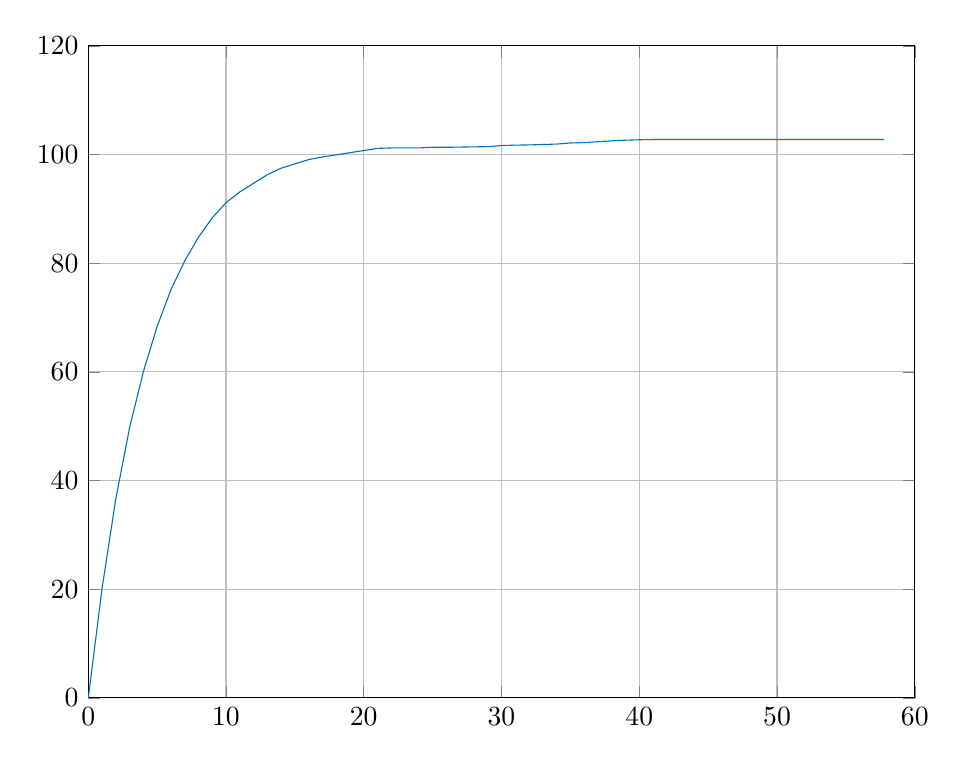
\begin{tikzpicture}

\begin{axis}[%
width=4.133in,
height=3.26in,
at={(0.693in,0.44in)},
scale only axis,
xmin=0,
xmax=60,
xmajorgrids,
ymin=0,
ymax=120,
ymajorgrids,
axis background/.style={fill=white}
]
\addplot [color=mycolor1,solid,forget plot]
  table[row sep=crcr]{%
0	0\\
0.0179118039999995	0.166\\
0.0330999039999992	0.446\\
0.048750436999999	0.754\\
0.0642097359999996	1.084\\
0.0798556380000003	1.4\\
0.0957486339999996	1.714\\
0.111709159	2.046\\
0.128792557	2.388\\
0.143668043	2.702\\
0.159576550999999	3.032\\
0.17766758	3.354\\
0.193047109999999	3.68\\
0.208477968999999	4.004\\
0.224017873	4.318\\
0.239796939999999	4.63\\
0.255747902999999	4.948\\
0.271881966	5.272\\
0.287974163999999	5.602\\
0.303747914999999	5.924\\
0.319712444	6.242\\
0.335854729	6.572\\
0.351747480999999	6.892\\
0.367800309999999	7.218\\
0.383669375	7.538\\
0.399585159	7.868\\
0.417663297999999	8.214\\
0.432459596999999	8.528\\
0.447867683	8.84\\
0.463873152999999	9.158\\
0.479865380999999	9.478\\
0.49588984	9.804\\
0.511904181	10.126\\
0.527763734999999	10.448\\
0.546094696999999	10.786\\
0.561157036999999	11.114\\
0.576219702	11.434\\
0.59172717	11.75\\
0.607834206999998	12.066\\
0.62366159	12.388\\
0.639634886	12.712\\
0.655714901999999	13.034\\
0.671695955	13.36\\
0.687711682	13.686\\
0.703612534	14.006\\
0.719698327	14.326\\
0.736002740999999	14.652\\
0.751813875	14.976\\
0.767909366999999	15.298\\
0.783930313999999	15.624\\
0.800050655999999	15.946\\
0.815986303999999	16.272\\
0.832080325999999	16.594\\
0.847988226	16.916\\
0.863913766999999	17.244\\
0.879877074999999	17.57\\
0.895577595999999	17.884\\
0.911638609999999	18.206\\
0.927615191	18.548\\
0.943710971999999	18.864\\
0.959570442	19.188\\
0.975702630999999	19.518\\
0.991700043	19.834\\
1.009233032	20.184\\
1.024242002	20.446\\
1.039625177	20.7\\
1.055652258	20.954\\
1.071681535	21.22\\
1.087710483	21.48\\
1.103754722	21.74\\
1.119887076	22.006\\
1.135594747	22.264\\
1.153729693	22.552\\
1.16916836	22.812\\
1.184356586	23.068\\
1.199697091	23.324\\
1.215674298	23.584\\
1.231682856	23.85\\
1.247679252	24.112\\
1.263696801	24.374\\
1.289572732	24.676\\
1.301487183	24.924\\
1.313492631	25.176\\
1.328740927	25.436\\
1.343984076	25.698\\
1.359730245	25.964\\
1.3758146	26.222\\
1.39162767	26.496\\
1.409796502	26.774\\
1.424920027	27.028\\
1.440080965	27.286\\
1.455833634	27.544\\
1.471752269	27.806\\
1.487773195	28.07\\
1.503740119	28.346\\
1.519802069	28.608\\
1.535762468	28.868\\
1.551716519	29.128\\
1.567808911	29.398\\
1.583746459	29.672\\
1.59974942	29.928\\
1.615872382	30.186\\
1.631697963	30.452\\
1.649047137	30.712\\
1.664102744	30.976\\
1.67974418	31.238\\
1.695760138	31.5\\
1.71173056	31.764\\
1.727680015	32.028\\
1.743756226	32.294\\
1.75974293	32.556\\
1.775762163	32.818\\
1.791757992	33.096\\
1.807767465	33.354\\
1.823749416	33.618\\
1.839725314	33.878\\
1.855729047	34.138\\
1.871830241	34.4\\
1.887669626	34.666\\
1.903622844	34.93\\
1.91976352	35.196\\
1.935733463	35.456\\
1.951787339	35.724\\
1.96784986	35.984\\
1.983760922	36.25\\
1.999939576	36.516\\
2.017738886	36.79\\
2.033098144	36.984\\
2.048565566	37.184\\
2.063921074	37.396\\
2.079841574	37.604\\
2.095839859	37.812\\
2.112164469	38.018\\
2.127597016	38.242\\
2.145672213	38.454\\
2.160545444	38.658\\
2.175783542	38.858\\
2.191777542	39.06\\
2.207728249	39.268\\
2.223755505	39.488\\
2.239721068	39.688\\
2.255758159	39.898\\
2.27174537	40.108\\
2.287828422	40.324\\
2.303741569	40.53\\
2.319736241	40.738\\
2.335766073	40.948\\
2.351754961	41.156\\
2.367692304	41.366\\
2.383743693	41.582\\
2.399636413	41.788\\
2.415701867	41.994\\
2.431671269	42.2\\
2.447618276	42.408\\
2.463595471	42.622\\
2.481712661	42.838\\
2.496685987	43.04\\
2.511589672	43.252\\
2.529687754	43.464\\
2.544618887	43.672\\
2.559816057	43.878\\
2.575729054	44.086\\
2.59173021	44.296\\
2.607775402	44.504\\
2.623950683	44.712\\
2.64041981	44.926\\
2.655715893	45.134\\
2.67157277	45.34\\
2.68757642	45.552\\
2.703720256	45.758\\
2.719739431	45.966\\
2.735704378	46.182\\
2.751758775	46.394\\
2.767730535	46.598\\
2.783797887	46.816\\
2.799767597	47.022\\
2.815714176	47.23\\
2.831713288	47.434\\
2.847718874	47.642\\
2.863683643	47.85\\
2.879642291	48.066\\
2.897697277	48.28\\
2.912492924	48.486\\
2.927737938	48.69\\
2.943795276	48.898\\
2.959766625	49.106\\
2.975871442	49.324\\
2.992099037	49.532\\
3.009693863	49.76\\
3.023716157	49.918\\
3.040118392	50.084\\
3.055924001	50.254\\
3.071909222	50.414\\
3.087919965	50.57\\
3.103938366	50.732\\
3.120334432	50.894\\
3.13700061	51.062\\
3.152441297	51.232\\
3.167885604	51.392\\
3.183928624	51.552\\
3.199777159	51.724\\
3.215747462	51.888\\
3.231893657	52.06\\
3.247758389	52.218\\
3.263776494	52.382\\
3.279734649	52.552\\
3.295738993	52.716\\
3.31411083	52.882\\
3.329270089	53.044\\
3.344457477	53.206\\
3.359778104	53.368\\
3.375782421	53.528\\
3.391591953	53.702\\
3.409730446	53.87\\
3.424901295	54.036\\
3.440078923	54.194\\
3.455908387	54.358\\
3.471667697	54.524\\
3.487579354	54.694\\
3.503841019	54.856\\
3.519709961	55.016\\
3.535807288	55.186\\
3.554187834	55.356\\
3.569433493	55.516\\
3.584727203	55.678\\
3.599879898	55.84\\
3.615773797	56.004\\
3.631774324	56.17\\
3.647630656	56.34\\
3.6637388	56.502\\
3.679862935	56.664\\
3.695661588	56.83\\
3.711743518	56.998\\
3.727712962	57.16\\
3.743711463	57.326\\
3.759656778	57.488\\
3.775853588	57.654\\
3.791816618	57.82\\
3.807959847	57.982\\
3.823973838	58.15\\
3.839775098	58.312\\
3.855904841	58.476\\
3.871847944	58.642\\
3.887789658	58.806\\
3.903742988	58.972\\
3.919629419	59.138\\
3.935711642	59.304\\
3.951699262	59.466\\
3.967729601	59.63\\
3.983730311	59.794\\
3.999758228	59.958\\
4.017143227	60.134\\
4.032110933	60.254\\
4.047655571	60.38\\
4.063630551	60.514\\
4.079590331	60.65\\
4.097794705	60.79\\
4.112840443	60.914\\
4.127919732	61.048\\
4.143715192	61.178\\
4.159674018	61.31\\
4.175702131	61.442\\
4.191690659	61.58\\
4.2076984	61.716\\
4.223611672	61.846\\
4.239615559	61.976\\
4.255610231	62.108\\
4.27161744	62.242\\
4.287753054	62.374\\
4.303854473	62.512\\
4.319837965	62.642\\
4.335867074	62.782\\
4.35188527	62.912\\
4.367909709	63.044\\
4.383730705	63.172\\
4.399728329	63.312\\
4.415860284	63.45\\
4.431726866	63.58\\
4.447690402	63.712\\
4.463704178	63.844\\
4.479863267	63.978\\
4.495879152	64.112\\
4.511874866	64.242\\
4.527914059	64.378\\
4.543856267	64.512\\
4.559714185	64.64\\
4.575718097	64.778\\
4.591790646	64.914\\
4.607656245	65.042\\
4.623797083	65.172\\
4.639806959	65.306\\
4.656027022	65.446\\
4.671864162	65.576\\
4.687786956	65.706\\
4.703919666	65.838\\
4.719850198	65.98\\
4.735720162	66.108\\
4.751872045	66.248\\
4.767844026	66.374\\
4.783792473	66.516\\
4.799594223	66.644\\
4.815879503	66.776\\
4.831853178	66.906\\
4.847872731	67.04\\
4.863882151	67.172\\
4.87983347	67.302\\
4.895714625	67.438\\
4.911703679	67.572\\
4.927723456	67.702\\
4.943780648	67.836\\
4.959809754	67.974\\
4.975920634	68.104\\
4.991814474	68.242\\
5.009259738	68.378\\
5.024627485	68.49\\
5.039848379	68.592\\
5.055630066	68.698\\
5.071673138	68.804\\
5.087746216	68.914\\
5.103860918	69.018\\
5.119667174	69.126\\
5.135550754	69.234\\
5.153771083	69.352\\
5.168833413	69.458\\
5.183875231	69.56\\
5.19977257	69.664\\
5.215708757	69.774\\
5.231688556	69.882\\
5.247682954	69.988\\
5.263902537	70.096\\
5.279697057	70.208\\
5.295745636	70.316\\
5.311777311	70.422\\
5.327679101	70.528\\
5.343795045	70.634\\
5.359832003	70.744\\
5.375956038	70.852\\
5.391700817	70.962\\
5.407728606	71.07\\
5.423841064	71.174\\
5.439783337	71.284\\
5.455783799	71.39\\
5.471773022	71.498\\
5.487689301	71.61\\
5.503596831	71.718\\
5.521804105	71.828\\
5.536927623	71.936\\
5.552073999	72.04\\
5.567949808	72.144\\
5.58372431	72.254\\
5.59976002	72.36\\
5.615702208	72.47\\
5.631833519	72.58\\
5.647631594	72.684\\
5.66374218	72.792\\
5.679729025	72.9\\
5.695717543	73.006\\
5.711647406	73.118\\
5.727745684	73.226\\
5.743659352	73.33\\
5.759711281	73.44\\
5.775738796	73.554\\
5.791720493	73.658\\
5.807713036	73.768\\
5.823709416	73.87\\
5.839698	73.978\\
5.855701833	74.086\\
5.871690786	74.194\\
5.887715486	74.3\\
5.903701534	74.412\\
5.919854128	74.522\\
5.935745466	74.63\\
5.951817901	74.74\\
5.967707178	74.844\\
5.983885325	74.95\\
5.99987674	75.06\\
6.017682554	75.168\\
6.033057142	75.246\\
6.048517754	75.328\\
6.063927266	75.416\\
6.079910361	75.498\\
6.095863289	75.584\\
6.111918528	75.668\\
6.127765295	75.75\\
6.143846708	75.832\\
6.159846952	75.92\\
6.175723326	76.004\\
6.191871276	76.09\\
6.207879854	76.172\\
6.223879091	76.266\\
6.239849609	76.348\\
6.255749	76.436\\
6.271695753	76.52\\
6.28772997	76.602\\
6.303733442	76.686\\
6.319700887	76.77\\
6.335763638	76.852\\
6.35171639	76.936\\
6.367701771	77.024\\
6.383857663	77.108\\
6.39968224	77.192\\
6.415696351	77.28\\
6.431692266	77.366\\
6.447700473	77.45\\
6.463715677	77.534\\
6.479740016	77.618\\
6.49576019	77.706\\
6.511735091	77.792\\
6.527715493	77.876\\
6.543701585	77.958\\
6.55969328	78.048\\
6.575672387	78.132\\
6.591693078	78.216\\
6.607716034	78.298\\
6.623837964	78.388\\
6.639729843	78.472\\
6.655702911	78.554\\
6.671724389	78.638\\
6.687818135	78.724\\
6.703901092	78.81\\
6.719892321	78.894\\
6.735868376	78.982\\
6.751880898	79.066\\
6.767798009	79.152\\
6.783724914	79.232\\
6.799823149	79.316\\
6.815728765	79.404\\
6.831964448	79.49\\
6.848084308	79.574\\
6.863860961	79.658\\
6.879776755	79.744\\
6.895783048	79.826\\
6.912001647	79.914\\
6.92792606	80.002\\
6.943876793	80.084\\
6.959877628	80.168\\
6.975856715	80.256\\
6.991861169	80.342\\
7.009693559	80.428\\
7.02491957	80.502\\
7.041321259	80.568\\
7.056979499	80.638\\
7.072373845	80.708\\
7.087908245	80.778\\
7.103897344	80.846\\
7.119910658	80.914\\
7.135863325	80.986\\
7.151918502	81.056\\
7.167887278	81.122\\
7.183845763	81.194\\
7.199943946	81.264\\
7.215878605	81.334\\
7.231923832	81.4\\
7.247876543	81.472\\
7.263944937	81.542\\
7.279923523	81.61\\
7.295886303	81.68\\
7.311892491	81.75\\
7.328546952	81.82\\
7.343954534	81.89\\
7.359905843	81.96\\
7.375810511	82.03\\
7.391707186	82.098\\
7.407665932	82.166\\
7.42369424	82.236\\
7.439698163	82.306\\
7.455894572	82.376\\
7.471987737	82.448\\
7.48788129	82.518\\
7.503728307	82.586\\
7.519679571	82.656\\
7.535717325	82.726\\
7.551922714	82.794\\
7.567940669	82.864\\
7.583847457	82.934\\
7.599724222	83.008\\
7.615939614	83.076\\
7.631924338	83.146\\
7.647869227	83.218\\
7.663875781	83.286\\
7.679887968	83.356\\
7.695872246	83.426\\
7.712029883	83.494\\
7.727823629	83.564\\
7.743717012	83.636\\
7.759693593	83.704\\
7.775699254	83.774\\
7.791713346	83.844\\
7.807695283	83.914\\
7.823858337	83.984\\
7.839886841	84.052\\
7.855742402	84.124\\
7.871736338	84.192\\
7.88775119	84.264\\
7.903890565	84.336\\
7.919691005	84.404\\
7.935719347	84.472\\
7.951811189	84.54\\
7.967643559	84.61\\
7.98375351	84.682\\
7.999752023	84.752\\
8.0172344	84.822\\
8.032501316	84.874\\
8.047637723	84.932\\
8.064008387	84.988\\
8.079890329	85.044\\
8.095943909	85.102\\
8.111866748	85.154\\
8.127792284	85.214\\
8.14377113	85.274\\
8.159872398	85.33\\
8.175859373	85.386\\
8.19188057	85.444\\
8.207744793	85.498\\
8.223646829	85.556\\
8.239699021	85.616\\
8.255700177	85.672\\
8.271754113	85.728\\
8.287822347	85.786\\
8.303729345	85.842\\
8.319706914	85.9\\
8.335718143	85.956\\
8.351746411	86.014\\
8.367740487	86.072\\
8.38370485	86.128\\
8.399856307	86.188\\
8.415710256	86.244\\
8.431708035	86.298\\
8.447868657	86.356\\
8.463921697	86.414\\
8.479767707	86.47\\
8.495879554	86.528\\
8.511934718	86.586\\
8.527904744	86.642\\
8.544041663	86.7\\
8.559885489	86.756\\
8.575874368	86.816\\
8.591872808	86.87\\
8.60772395	86.928\\
8.623806005	86.984\\
8.639760941	87.042\\
8.655905137	87.096\\
8.671887576	87.156\\
8.68786961	87.214\\
8.703890707	87.27\\
8.720257857	87.326\\
8.735929247	87.384\\
8.751905748	87.442\\
8.767909846	87.498\\
8.78385459	87.556\\
8.799874509	87.614\\
8.81583359	87.672\\
8.831717877	87.73\\
8.847698538	87.782\\
8.863700476	87.84\\
8.879781484	87.896\\
8.895712967	87.954\\
8.911792003	88.01\\
8.927860996	88.07\\
8.943896801	88.126\\
8.959865123	88.184\\
8.975883985	88.24\\
8.991911206	88.296\\
9.007731793	88.354\\
9.023915709	88.404\\
9.039890796	88.444\\
9.055831479	88.488\\
9.071689904	88.53\\
9.08785604	88.576\\
9.103896671	88.62\\
9.11973996	88.666\\
9.135812308	88.708\\
9.151856572	88.754\\
9.167694078	88.8\\
9.183822423	88.844\\
9.199635107	88.886\\
9.215768449	88.932\\
9.231860997	88.976\\
9.247786783	89.02\\
9.263889299	89.066\\
9.279792875	89.108\\
9.295761815	89.154\\
9.311779438	89.196\\
9.327953719	89.244\\
9.343892386	89.288\\
9.35974016	89.334\\
9.375845964	89.376\\
9.391769225	89.422\\
9.407621223	89.466\\
9.423829459	89.51\\
9.439598515	89.554\\
9.455897175	89.596\\
9.471797574	89.642\\
9.487734622	89.686\\
9.503754424	89.732\\
9.519864277	89.776\\
9.53576403	89.818\\
9.551704846	89.866\\
9.567757076	89.906\\
9.583762668	89.954\\
9.599740817	89.996\\
9.615699969	90.042\\
9.631913291	90.086\\
9.647748452	90.13\\
9.663720497	90.178\\
9.679720747	90.22\\
9.695744029	90.264\\
9.711697483	90.306\\
9.727765345	90.352\\
9.743725815	90.396\\
9.759728941	90.44\\
9.775734382	90.486\\
9.791826931	90.53\\
9.807746327	90.576\\
9.82371695	90.618\\
9.839969806	90.664\\
9.855889889	90.708\\
9.871885473	90.754\\
9.887870379	90.798\\
9.903941915	90.842\\
9.919940802	90.886\\
9.935812715	90.928\\
9.951856308	90.976\\
9.967908926	91.018\\
9.983885467	91.062\\
9.999870507	91.108\\
10.017515586	91.154\\
10.0330492	91.18\\
10.048517575	91.21\\
10.063966593	91.244\\
10.079901928	91.276\\
10.095876344	91.306\\
10.111721629	91.338\\
10.127886886	91.368\\
10.143933757	91.4\\
10.159870221	91.434\\
10.175857757	91.466\\
10.191729761	91.498\\
10.207701817	91.528\\
10.223753553	91.56\\
10.239764768	91.59\\
10.25575062	91.624\\
10.271769792	91.654\\
10.287769928	91.688\\
10.303671245	91.718\\
10.319759326	91.748\\
10.335801876	91.778\\
10.351792163	91.814\\
10.367868525	91.844\\
10.383722057	91.878\\
10.399643539	91.908\\
10.415919202	91.938\\
10.431763072	91.97\\
10.447756326	92.006\\
10.463703831	92.036\\
10.479751127	92.068\\
10.495690885	92.098\\
10.511704494	92.128\\
10.527721674	92.158\\
10.543649052	92.194\\
10.559795979	92.224\\
10.575710991	92.258\\
10.591701207	92.288\\
10.607691915	92.318\\
10.623792402	92.35\\
10.640954819	92.384\\
10.656163586	92.414\\
10.671952893	92.448\\
10.687835501	92.478\\
10.703741783	92.508\\
10.719677431	92.542\\
10.735707207	92.574\\
10.751734749	92.606\\
10.767734171	92.638\\
10.783758039	92.67\\
10.799733473	92.7\\
10.815718989	92.732\\
10.831687702	92.764\\
10.847805969	92.796\\
10.863925013	92.828\\
10.879838305	92.858\\
10.89588046	92.888\\
10.911907405	92.926\\
10.927931168	92.956\\
10.943852228	92.988\\
10.959890083	93.02\\
10.975881843	93.05\\
10.991753566	93.08\\
11.009408716	93.116\\
11.024746741	93.14\\
11.039924311	93.166\\
11.055677357	93.19\\
11.071685309	93.214\\
11.090163772	93.244\\
11.105435934	93.266\\
11.120604471	93.29\\
11.135821566	93.316\\
11.151807659	93.34\\
11.167915013	93.368\\
11.18363109	93.392\\
11.202018284	93.418\\
11.217192347	93.444\\
11.232399946	93.468\\
11.247780321	93.494\\
11.264021196	93.52\\
11.279791795	93.546\\
11.295852738	93.57\\
11.311744146	93.596\\
11.327677358	93.622\\
11.343765963	93.646\\
11.359748668	93.672\\
11.375836391	93.698\\
11.391635698	93.72\\
11.407760487	93.748\\
11.423705857	93.772\\
11.439779653	93.8\\
11.455756214	93.822\\
11.471626148	93.85\\
11.487732388	93.874\\
11.503738466	93.9\\
11.519737929	93.928\\
11.535729925	93.95\\
11.551744667	93.976\\
11.567777485	94\\
11.58373815	94.026\\
11.599893176	94.05\\
11.615916673	94.08\\
11.63182139	94.102\\
11.648136392	94.132\\
11.663866212	94.152\\
11.679835615	94.18\\
11.695885943	94.206\\
11.712047428	94.23\\
11.727712559	94.256\\
11.743710333	94.28\\
11.759691254	94.306\\
11.775706086	94.33\\
11.792020252	94.356\\
11.807652267	94.38\\
11.823691024	94.408\\
11.839700725	94.432\\
11.855811039	94.458\\
11.871717706	94.484\\
11.88777132	94.512\\
11.903687416	94.536\\
11.919764595	94.56\\
11.935799487	94.586\\
11.951755317	94.61\\
11.96777037	94.636\\
11.983826426	94.66\\
11.999702692	94.686\\
12.017246742	94.716\\
12.032372119	94.74\\
12.047717255	94.762\\
12.063725633	94.79\\
12.079728583	94.812\\
12.095737984	94.838\\
12.111701145	94.864\\
12.127716704	94.89\\
12.144029687	94.916\\
12.159859786	94.94\\
12.175727555	94.966\\
12.191705014	94.99\\
12.207700157	95.016\\
12.22366685	95.04\\
12.239697218	95.068\\
12.255797724	95.09\\
12.271697056	95.118\\
12.287720643	95.142\\
12.303666765	95.168\\
12.319667195	95.192\\
12.335745757	95.22\\
12.351730897	95.246\\
12.367729473	95.27\\
12.38357457	95.298\\
12.401623232	95.32\\
12.416410069	95.346\\
12.431831755	95.37\\
12.447728732	95.398\\
12.463697906	95.42\\
12.479777846	95.448\\
12.495915146	95.474\\
12.512208048	95.498\\
12.527857849	95.524\\
12.543877172	95.55\\
12.559855812	95.574\\
12.575873782	95.6\\
12.591844595	95.624\\
12.607836892	95.65\\
12.623853183	95.678\\
12.639589795	95.7\\
12.655821008	95.728\\
12.671754236	95.75\\
12.687703966	95.778\\
12.703690309	95.802\\
12.719816759	95.828\\
12.735880358	95.852\\
12.751723651	95.88\\
12.767698073	95.904\\
12.783679209	95.93\\
12.79964918	95.954\\
12.81586833	95.98\\
12.831968837	96.008\\
12.847852533	96.03\\
12.863747779	96.056\\
12.87988732	96.08\\
12.895600268	96.108\\
12.911678399	96.13\\
12.927869636	96.158\\
12.943837738	96.182\\
12.960029557	96.208\\
12.975933228	96.234\\
12.991754436	96.26\\
13.009294434	96.284\\
13.024322632	96.304\\
13.039722802	96.322\\
13.055636918	96.342\\
13.071654545	96.362\\
13.08770087	96.382\\
13.103691998	96.4\\
13.119853478	96.42\\
13.135790827	96.438\\
13.151787091	96.454\\
13.167875315	96.474\\
13.183871761	96.494\\
13.199760673	96.514\\
13.215888477	96.532\\
13.23186162	96.552\\
13.247863433	96.572\\
13.263904044	96.59\\
13.279839722	96.612\\
13.2958941	96.632\\
13.311839244	96.644\\
13.327777037	96.662\\
13.343762248	96.682\\
13.359696027	96.702\\
13.375700341	96.722\\
13.391771172	96.742\\
13.407816615	96.762\\
13.423714866	96.782\\
13.439682136	96.8\\
13.455676487	96.82\\
13.471863855	96.836\\
13.487791876	96.854\\
13.503781471	96.872\\
13.51969948	96.892\\
13.535711667	96.912\\
13.551697699	96.932\\
13.567663796	96.952\\
13.583669087	96.972\\
13.599911746	96.99\\
13.615941863	97.01\\
13.631871423	97.026\\
13.649431103	97.046\\
13.664349895	97.062\\
13.679802113	97.082\\
13.695696046	97.102\\
13.711768595	97.122\\
13.727890755	97.142\\
13.743981605	97.162\\
13.759871655	97.182\\
13.775946624	97.202\\
13.791879737	97.216\\
13.807824004	97.234\\
13.82354873	97.254\\
13.839966996	97.272\\
13.855907215	97.292\\
13.872018742	97.312\\
13.887689072	97.332\\
13.903547537	97.352\\
13.919845917	97.372\\
13.936194005	97.39\\
13.951889689	97.41\\
13.967712671	97.428\\
13.983613422	97.444\\
13.999691828	97.464\\
14.017205561	97.484\\
14.032349641	97.492\\
14.047684003	97.508\\
14.063872464	97.52\\
14.079724513	97.532\\
14.095706075	97.542\\
14.111643026	97.558\\
14.128105523	97.572\\
14.143591773	97.582\\
14.16178708	97.592\\
14.176883677	97.612\\
14.192164733	97.622\\
14.207702806	97.632\\
14.223694686	97.646\\
14.239851696	97.658\\
14.255875278	97.672\\
14.271858094	97.682\\
14.287871894	97.698\\
14.30391918	97.712\\
14.319883127	97.722\\
14.336746612	97.732\\
14.352219292	97.748\\
14.367901706	97.762\\
14.383896208	97.772\\
14.399788057	97.782\\
14.41577872	97.8\\
14.43194457	97.812\\
14.447851242	97.822\\
14.46372942	97.836\\
14.479707354	97.85\\
14.495708766	97.862\\
14.511717776	97.872\\
14.527660385	97.888\\
14.543876323	97.902\\
14.559911421	97.912\\
14.575894903	97.922\\
14.591883566	97.938\\
14.607884863	97.952\\
14.623719909	97.962\\
14.639609542	97.974\\
14.655752866	97.99\\
14.671923557	98.002\\
14.687964796	98.012\\
14.703733953	98.026\\
14.719740047	98.04\\
14.73569278	98.052\\
14.751933099	98.062\\
14.767874135	98.078\\
14.783699671	98.092\\
14.799769661	98.102\\
14.81572787	98.112\\
14.831684626	98.128\\
14.847691816	98.142\\
14.86370698	98.152\\
14.880019853	98.168\\
14.895766127	98.18\\
14.911838046	98.192\\
14.927887986	98.202\\
14.943878914	98.216\\
14.959902367	98.232\\
14.97584461	98.242\\
14.991720939	98.252\\
15.009126537	98.27\\
15.0242078	98.282\\
15.039844861	98.292\\
15.055865983	98.306\\
15.071731282	98.318\\
15.087724266	98.332\\
15.103708078	98.342\\
15.119691544	98.356\\
15.135774552	98.37\\
15.15163189	98.382\\
15.167734655	98.392\\
15.183834089	98.408\\
15.199784505	98.422\\
15.215698252	98.432\\
15.231874026	98.442\\
15.2481038	98.458\\
15.263895197	98.472\\
15.279825122	98.482\\
15.295896338	98.494\\
15.311809956	98.51\\
15.327865741	98.522\\
15.343860529	98.532\\
15.359872184	98.546\\
15.375869216	98.562\\
15.3917786	98.572\\
15.407866568	98.582\\
15.423807659	98.598\\
15.439718521	98.612\\
15.455862151	98.622\\
15.471905905	98.634\\
15.487874026	98.648\\
15.503798012	98.662\\
15.519844982	98.672\\
15.53591262	98.686\\
15.55206762	98.702\\
15.567705855	98.712\\
15.58367997	98.722\\
15.599709361	98.738\\
15.615956044	98.752\\
15.631898337	98.762\\
15.647816846	98.774\\
15.663853819	98.788\\
15.679866387	98.802\\
15.695723141	98.812\\
15.711869296	98.824\\
15.727922937	98.838\\
15.743860379	98.852\\
15.759845128	98.862\\
15.776012231	98.876\\
15.791918588	98.892\\
15.807882154	98.902\\
15.823892011	98.912\\
15.839798557	98.928\\
15.855852123	98.942\\
15.871870348	98.952\\
15.887846907	98.962\\
15.903923601	98.978\\
15.919878947	98.992\\
15.935726635	99.004\\
15.95169441	99.016\\
15.967883117	99.028\\
15.983904319	99.042\\
15.999887725	99.052\\
16.017617192	99.064\\
16.032884211	99.074\\
16.048349103	99.082\\
16.063765675	99.086\\
16.079957017	99.096\\
16.095858478	99.104\\
16.111853456	99.11\\
16.127862811	99.12\\
16.143847945	99.124\\
16.159744335	99.134\\
16.175717344	99.142\\
16.191665721	99.148\\
16.207702668	99.158\\
16.223577439	99.166\\
16.239874606	99.17\\
16.255880273	99.18\\
16.271887438	99.186\\
16.287845928	99.194\\
16.303898316	99.202\\
16.319873183	99.208\\
16.336931865	99.218\\
16.352462691	99.226\\
16.367841177	99.23\\
16.383755758	99.24\\
16.39968624	99.25\\
16.415879161	99.254\\
16.431779022	99.264\\
16.447869304	99.272\\
16.463873996	99.278\\
16.479937754	99.286\\
16.495853277	99.292\\
16.511878508	99.302\\
16.528071479	99.31\\
16.543920406	99.314\\
16.559947512	99.324\\
16.575858178	99.334\\
16.591884722	99.338\\
16.607935096	99.346\\
16.623873099	99.352\\
16.639860599	99.362\\
16.655778127	99.37\\
16.671706574	99.376\\
16.687615455	99.386\\
16.703883182	99.394\\
16.719875529	99.398\\
16.735907089	99.408\\
16.751875166	99.416\\
16.767879414	99.422\\
16.783874066	99.43\\
16.79984752	99.436\\
16.81586113	99.446\\
16.83172235	99.454\\
16.847697793	99.458\\
16.863874102	99.468\\
16.879891119	99.478\\
16.895595481	99.482\\
16.913822688	99.492\\
16.929289554	99.5\\
16.944775602	99.506\\
16.960260245	99.514\\
16.97590725	99.52\\
16.99185899	99.53\\
17.009827788	99.538\\
17.025435118	99.54\\
17.040998914	99.55\\
17.056208362	99.558\\
17.071714487	99.56\\
17.087697363	99.57\\
17.103857565	99.572\\
17.119885246	99.58\\
17.135830592	99.588\\
17.151824334	99.592\\
17.167756577	99.6\\
17.183855109	99.608\\
17.19993551	99.61\\
17.215960822	99.62\\
17.231718903	99.628\\
17.247701542	99.63\\
17.263715854	99.64\\
17.279702818	99.642\\
17.295702181	99.65\\
17.31166892	99.658\\
17.327768935	99.66\\
17.343750618	99.67\\
17.359730686	99.678\\
17.375723048	99.68\\
17.39162808	99.69\\
17.407577538	99.694\\
17.426021642	99.7\\
17.441645674	99.71\\
17.456755036	99.712\\
17.471760412	99.72\\
17.487709767	99.728\\
17.50369187	99.73\\
17.519871265	99.74\\
17.536064196	99.748\\
17.55186102	99.75\\
17.567853156	99.76\\
17.583891623	99.764\\
17.599857604	99.77\\
17.615868844	99.778\\
17.632084411	99.782\\
17.647645068	99.79\\
17.66370948	99.798\\
17.679693593	99.8\\
17.695707834	99.81\\
17.711801586	99.818\\
17.727693179	99.82\\
17.743724374	99.83\\
17.759667389	99.832\\
17.775882735	99.84\\
17.791897959	99.848\\
17.807851979	99.852\\
17.823897551	99.86\\
17.839895436	99.868\\
17.855876296	99.87\\
17.871872917	99.88\\
17.887806141	99.888\\
17.90383978	99.89\\
17.919800987	99.9\\
17.935864003	99.904\\
17.951623751	99.91\\
17.968873809	99.918\\
17.984128818	99.92\\
17.999642604	99.93\\
18.017873375	99.938\\
18.033269291	99.94\\
18.048411626	99.95\\
18.063734134	99.958\\
18.079746832	99.96\\
18.095612544	99.968\\
18.111811268	99.972\\
18.127933342	99.98\\
18.145389837	99.988\\
18.160632541	99.99\\
18.175741744	100\\
18.191763768	100.008\\
18.207694513	100.01\\
18.223724233	100.02\\
18.239790513	100.026\\
18.255764348	100.03\\
18.271715527	100.038\\
18.287776734	100.042\\
18.303725277	100.05\\
18.319848545	100.058\\
18.335898157	100.06\\
18.351863793	100.07\\
18.367917343	100.078\\
18.383875868	100.08\\
18.399630798	100.09\\
18.415582664	100.092\\
18.433571702	100.1\\
18.44862872	100.108\\
18.463687361	100.112\\
18.47960983	100.12\\
18.495701191	100.128\\
18.513972835	100.13\\
18.529287592	100.14\\
18.544704095	100.148\\
18.560097279	100.15\\
18.576031709	100.158\\
18.5917413	100.162\\
18.607656141	100.17\\
18.623839386	100.178\\
18.639831079	100.18\\
18.655585027	100.19\\
18.673627298	100.198\\
18.688690866	100.202\\
18.703934091	100.212\\
18.719701518	100.216\\
18.735665515	100.222\\
18.751876286	100.232\\
18.767872622	100.234\\
18.783859256	100.242\\
18.799917206	100.252\\
18.815857374	100.252\\
18.831946782	100.262\\
18.847854887	100.27\\
18.864023157	100.272\\
18.879899692	100.282\\
18.895639341	100.284\\
18.911732948	100.292\\
18.927842083	100.302\\
18.943842358	100.304\\
18.959791006	100.312\\
18.975855204	100.32\\
18.991883939	100.324\\
19.009772454	100.332\\
19.025223887	100.34\\
19.040585245	100.342\\
19.056239345	100.352\\
19.07188861	100.356\\
19.08786718	100.362\\
19.103794129	100.372\\
19.119839942	100.374\\
19.135818492	100.382\\
19.152066213	100.39\\
19.167844349	100.392\\
19.183784272	100.402\\
19.199853926	100.41\\
19.215665	100.412\\
19.231715277	100.422\\
19.247870388	100.424\\
19.263891382	100.432\\
19.279961733	100.44\\
19.295675195	100.444\\
19.311811079	100.452\\
19.327691292	100.46\\
19.343817003	100.462\\
19.359833071	100.472\\
19.375764927	100.478\\
19.391699555	100.482\\
19.407698209	100.492\\
19.423676103	100.494\\
19.439739526	100.502\\
19.455675759	100.51\\
19.472028913	100.512\\
19.48769148	100.522\\
19.503791884	100.53\\
19.519706164	100.532\\
19.53573347	100.542\\
19.551766594	100.546\\
19.567758731	100.552\\
19.583834146	100.562\\
19.599614216	100.566\\
19.61786122	100.572\\
19.633015448	100.58\\
19.648347818	100.582\\
19.663652471	100.592\\
19.679792375	100.6\\
19.695648628	100.602\\
19.711736541	100.612\\
19.727739435	100.614\\
19.743762299	100.622\\
19.759774309	100.632\\
19.775828987	100.634\\
19.791677672	100.642\\
19.807809584	100.65\\
19.823730208	100.652\\
19.839675374	100.662\\
19.855655555	100.67\\
19.871713053	100.672\\
19.887757973	100.682\\
19.903705895	100.684\\
19.919889205	100.692\\
19.935762727	100.702\\
19.95181536	100.704\\
19.968041089	100.712\\
19.983702619	100.722\\
20.000001615	100.722\\
20.017602735	100.732\\
20.032825448	100.74\\
20.048073124	100.742\\
20.063643053	100.752\\
20.081935157	100.756\\
20.097175633	100.762\\
20.112482884	100.77\\
20.127833676	100.772\\
20.143682536	100.782\\
20.159609123	100.79\\
20.177580923	100.792\\
20.192555477	100.802\\
20.207851792	100.806\\
20.223730351	100.812\\
20.239712936	100.822\\
20.255914136	100.824\\
20.271907269	100.832\\
20.287859715	100.84\\
20.303909803	100.844\\
20.319853935	100.852\\
20.335867049	100.86\\
20.352394618	100.862\\
20.367729981	100.872\\
20.383780751	100.874\\
20.399599573	100.882\\
20.417663093	100.892\\
20.433217112	100.894\\
20.448750353	100.902\\
20.464386763	100.91\\
20.480035888	100.912\\
20.495896787	100.922\\
20.51190077	100.93\\
20.528153772	100.932\\
20.543997918	100.942\\
20.559903713	100.944\\
20.575872206	100.952\\
20.591842207	100.96\\
20.607949815	100.962\\
20.623882531	100.972\\
20.639687998	100.98\\
20.655591043	100.982\\
20.673702826	100.992\\
20.688875968	101\\
20.703918924	101.002\\
20.719707444	101.012\\
20.735704196	101.014\\
20.751719219	101.022\\
20.767691104	101.03\\
20.783756967	101.034\\
20.799693137	101.042\\
20.815716519	101.05\\
20.831641805	101.052\\
20.847637385	101.062\\
20.863640346	101.066\\
20.879609913	101.072\\
20.895588428	101.082\\
20.913686254	101.084\\
20.929125203	101.092\\
20.944540949	101.1\\
20.959997687	101.104\\
20.976018203	101.112\\
20.991795266	101.12\\
21.00943077	101.12\\
21.024805262	101.126\\
21.040425005	101.128\\
21.055888213	101.128\\
21.071865846	101.13\\
21.087737249	101.13\\
21.103964423	101.132\\
21.119876883	101.134\\
21.135792191	101.134\\
21.151650917	101.136\\
21.169683786	101.138\\
21.185140162	101.138\\
21.200718478	101.14\\
21.216276723	101.14\\
21.232058914	101.142\\
21.247877302	101.144\\
21.263886176	101.144\\
21.279725656	101.146\\
21.295873891	101.148\\
21.311879423	101.148\\
21.32780589	101.15\\
21.343630782	101.152\\
21.359810854	101.152\\
21.375607683	101.154\\
21.391593474	101.154\\
21.407738943	101.156\\
21.423597912	101.158\\
21.439762866	101.158\\
21.455828438	101.16\\
21.471839437	101.162\\
21.48771552	101.162\\
21.503705517	101.164\\
21.519708799	101.164\\
21.535732887	101.166\\
21.551597562	101.168\\
21.567702702	101.168\\
21.583695077	101.17\\
21.599759414	101.172\\
21.615729264	101.172\\
21.631746655	101.174\\
21.647687553	101.176\\
21.665841085	101.176\\
21.681128054	101.178\\
21.696538377	101.178\\
21.711885327	101.18\\
21.727871389	101.182\\
21.743884798	101.182\\
21.759960945	101.184\\
21.775867082	101.186\\
21.791850939	101.186\\
21.807895058	101.188\\
21.82388092	101.19\\
21.839842532	101.19\\
21.855957647	101.192\\
21.871880817	101.192\\
21.887821782	101.194\\
21.903604482	101.196\\
21.921751857	101.196\\
21.937330842	101.198\\
21.95276558	101.2\\
21.968163561	101.2\\
21.983925276	101.202\\
21.999933012	101.204\\
22.017373349	101.204\\
22.032437439	101.204\\
22.048008174	101.204\\
22.063886287	101.204\\
22.079976045	101.204\\
22.095839965	101.204\\
22.111878376	101.204\\
22.127857012	101.204\\
22.143764697	101.204\\
22.159584096	101.204\\
22.175843704	101.204\\
22.191937716	101.204\\
22.207885717	101.204\\
22.223897227	101.204\\
22.239724886	101.204\\
22.255702404	101.204\\
22.271700694	101.204\\
22.287707864	101.204\\
22.30368191	101.204\\
22.319879657	101.204\\
22.335927604	101.204\\
22.351888069	101.204\\
22.367876231	101.204\\
22.383905692	101.204\\
22.399605249	101.204\\
22.417814053	101.204\\
22.432966148	101.204\\
22.448326581	101.204\\
22.46382437	101.204\\
22.479897067	101.204\\
22.495887574	101.204\\
22.511927935	101.204\\
22.527905723	101.204\\
22.543850512	101.204\\
22.559711551	101.204\\
22.575695995	101.204\\
22.591703481	101.204\\
22.607865986	101.204\\
22.623905352	101.204\\
22.639873638	101.204\\
22.655597611	101.204\\
22.671770789	101.204\\
22.68765072	101.204\\
22.703651772	101.204\\
22.719548501	101.204\\
22.73552303	101.204\\
22.753852199	101.204\\
22.769442001	101.204\\
22.784860385	101.204\\
22.80031133	101.204\\
22.815900113	101.204\\
22.831871457	101.204\\
22.847950685	101.204\\
22.863873665	101.204\\
22.879836284	101.204\\
22.895676329	101.204\\
22.911589822	101.204\\
22.929679006	101.204\\
22.94522009	101.204\\
22.960864018	101.204\\
22.976430524	101.204\\
22.99192109	101.204\\
23.009444665	101.204\\
23.024899143	101.204\\
23.040560771	101.204\\
23.056173588	101.204\\
23.071970893	101.204\\
23.087892554	101.204\\
23.10381388	101.204\\
23.119756253	101.204\\
23.135816689	101.204\\
23.15159341	101.204\\
23.169774683	101.204\\
23.184841283	101.204\\
23.199949541	101.204\\
23.21585219	101.204\\
23.231747146	101.204\\
23.247770142	101.204\\
23.263875405	101.204\\
23.279748746	101.204\\
23.295925401	101.204\\
23.311892881	101.204\\
23.327791786	101.204\\
23.343895766	101.204\\
23.359865406	101.204\\
23.376237448	101.204\\
23.392914918	101.204\\
23.409325726	101.204\\
23.424438696	101.204\\
23.439677566	101.204\\
23.455687151	101.204\\
23.47193035	101.204\\
23.487895421	101.204\\
23.503767272	101.204\\
23.519783786	101.204\\
23.53583242	101.204\\
23.551810515	101.204\\
23.56774802	101.204\\
23.583839679	101.204\\
23.599761576	101.204\\
23.615682842	101.204\\
23.631840689	101.204\\
23.648958896	101.204\\
23.663995387	101.204\\
23.679796736	101.204\\
23.69563078	101.204\\
23.714069558	101.204\\
23.729307616	101.204\\
23.74463454	101.204\\
23.759922693	101.204\\
23.776051156	101.204\\
23.791915561	101.204\\
23.80761041	101.204\\
23.825761052	101.204\\
23.83958801	101.204\\
23.855584616	101.204\\
23.871765673	101.204\\
23.887675353	101.204\\
23.903594072	101.204\\
23.919599123	101.204\\
23.937696905	101.204\\
23.953388856	101.204\\
23.968548367	101.204\\
23.983862812	101.204\\
23.999751269	101.204\\
24.017393212	101.206\\
24.032373421	101.206\\
24.047705221	101.206\\
24.063705285	101.212\\
24.079688968	101.212\\
24.09569277	101.212\\
24.111704581	101.218\\
24.127700871	101.218\\
24.143816858	101.218\\
24.15958336	101.222\\
24.177831164	101.224\\
24.192877192	101.224\\
24.207904493	101.228\\
24.22385778	101.23\\
24.240170493	101.23\\
24.255825257	101.232\\
24.271783446	101.236\\
24.287888862	101.236\\
24.303858118	101.238\\
24.319622221	101.242\\
24.335799544	101.242\\
24.35201549	101.242\\
24.367777661	101.248\\
24.383785148	101.248\\
24.399616088	101.248\\
24.415791139	101.254\\
24.431778434	101.254\\
24.447850987	101.254\\
24.463812378	101.258\\
24.479739858	101.26\\
24.495784584	101.26\\
24.511626566	101.264\\
24.527714529	101.266\\
24.543793959	101.266\\
24.559728072	101.27\\
24.575754736	101.272\\
24.591742758	101.272\\
24.607732329	101.274\\
24.623641281	101.278\\
24.641714596	101.278\\
24.656703064	101.28\\
24.671735803	101.284\\
24.687720582	101.284\\
24.703694762	101.284\\
24.719723953	101.29\\
24.735700965	101.29\\
24.751875359	101.29\\
24.767908267	101.296\\
24.78387458	101.296\\
24.799830143	101.296\\
24.815918016	101.3\\
24.831775177	101.302\\
24.847721023	101.302\\
24.863895848	101.306\\
24.879800677	101.308\\
24.895836146	101.308\\
24.911798124	101.31\\
24.927871499	101.314\\
24.943941381	101.314\\
24.959781503	101.314\\
24.975749715	101.32\\
24.991731153	101.32\\
25.00911015	101.32\\
25.024216615	101.322\\
25.039745321	101.322\\
25.055747486	101.322\\
25.071705655	101.322\\
25.087692624	101.322\\
25.103749322	101.322\\
25.11974028	101.322\\
25.135735243	101.322\\
25.151598312	101.322\\
25.169834947	101.322\\
25.185081328	101.322\\
25.200361252	101.322\\
25.215784369	101.322\\
25.231873675	101.322\\
25.247867224	101.322\\
25.263785379	101.322\\
25.279857862	101.322\\
25.295906035	101.322\\
25.311900401	101.322\\
25.329255826	101.322\\
25.3447529	101.322\\
25.360167247	101.322\\
25.37592143	101.322\\
25.39182464	101.322\\
25.407660257	101.322\\
25.423819531	101.322\\
25.439752348	101.322\\
25.455729811	101.322\\
25.471737708	101.322\\
25.487624656	101.322\\
25.503734303	101.322\\
25.519750263	101.322\\
25.535740399	101.322\\
25.551869662	101.322\\
25.567892263	101.322\\
25.583845631	101.322\\
25.599871849	101.322\\
25.615797284	101.322\\
25.631847863	101.322\\
25.64773911	101.322\\
25.664781561	101.322\\
25.679929902	101.322\\
25.695804847	101.322\\
25.711875215	101.322\\
25.727606334	101.322\\
25.745750759	101.322\\
25.761221991	101.322\\
25.776361502	101.322\\
25.792008005	101.322\\
25.807655346	101.322\\
25.823694384	101.322\\
25.839749722	101.322\\
25.855761911	101.322\\
25.871763548	101.322\\
25.889133104	101.322\\
25.904173128	101.322\\
25.919706014	101.322\\
25.935900423	101.322\\
25.951810258	101.322\\
25.970288391	101.322\\
25.985430777	101.322\\
26.000686898	101.322\\
26.015838565	101.322\\
26.032150555	101.322\\
26.047890424	101.324\\
26.063914217	101.324\\
26.079758384	101.324\\
26.09570337	101.326\\
26.111654858	101.326\\
26.127792524	101.326\\
26.143803177	101.328\\
26.159684265	101.328\\
26.175721223	101.328\\
26.191699332	101.33\\
26.207694305	101.33\\
26.224005479	101.33\\
26.239683175	101.332\\
26.255764852	101.332\\
26.271719559	101.332\\
26.287670702	101.332\\
26.303786782	101.334\\
26.319817026	101.334\\
26.335684389	101.334\\
26.351658579	101.336\\
26.367613061	101.336\\
26.383653418	101.336\\
26.39957372	101.338\\
26.4176804	101.338\\
26.432619669	101.338\\
26.447618205	101.34\\
26.465715642	101.34\\
26.480758096	101.34\\
26.495773199	101.342\\
26.511726782	101.342\\
26.528126306	101.342\\
26.543652518	101.344\\
26.559611364	101.344\\
26.575727267	101.344\\
26.591615011	101.346\\
26.607694554	101.346\\
26.6236173	101.346\\
26.639750411	101.346\\
26.655586443	101.348\\
26.673713939	101.348\\
26.689123947	101.348\\
26.703600618	101.35\\
26.719574477	101.35\\
26.735625125	101.35\\
26.751671293	101.352\\
26.767626696	101.352\\
26.783691393	101.352\\
26.799616152	101.354\\
26.815583459	101.354\\
26.831592495	101.354\\
26.8477035	101.356\\
26.863614197	101.356\\
26.879656769	101.356\\
26.895627417	101.358\\
26.911638717	101.358\\
26.929675708	101.358\\
26.944542145	101.36\\
26.959620467	101.36\\
26.975606522	101.36\\
26.991679932	101.36\\
27.009325575	101.362\\
27.024672085	101.362\\
27.039772082	101.364\\
27.055576274	101.364\\
27.073773046	101.364\\
27.087686803	101.366\\
27.103766637	101.366\\
27.119747355	101.366\\
27.135673422	101.366\\
27.151592043	101.368\\
27.167742713	101.368\\
27.18368919	101.368\\
27.199769425	101.37\\
27.215656017	101.37\\
27.231775466	101.37\\
27.247679593	101.372\\
27.263708878	101.372\\
27.279752998	101.372\\
27.295744146	101.374\\
27.311706034	101.374\\
27.327743874	101.374\\
27.343886837	101.376\\
27.359816947	101.376\\
27.375835148	101.376\\
27.391783645	101.378\\
27.407807082	101.378\\
27.423842351	101.378\\
27.439773335	101.38\\
27.455748401	101.38\\
27.471813728	101.38\\
27.487734398	101.38\\
27.503857791	101.382\\
27.519708103	101.382\\
27.538214117	101.382\\
27.553370169	101.384\\
27.568491367	101.384\\
27.583827848	101.384\\
27.599690227	101.386\\
27.615764794	101.386\\
27.631741164	101.386\\
27.647813231	101.388\\
27.663751631	101.388\\
27.679888946	101.388\\
27.695723385	101.39\\
27.711754359	101.39\\
27.727778588	101.39\\
27.743764806	101.392\\
27.759772553	101.392\\
27.775867051	101.392\\
27.792188688	101.392\\
27.807770364	101.394\\
27.823823699	101.394\\
27.839777308	101.394\\
27.855773419	101.396\\
27.871734409	101.396\\
27.887769688	101.396\\
27.903631334	101.398\\
27.919599413	101.398\\
27.935716209	101.398\\
27.951797472	101.4\\
27.967904935	101.4\\
27.983736184	101.4\\
27.999845543	101.402\\
28.017308762	101.402\\
28.03260528	101.402\\
28.047899187	101.402\\
28.063784922	101.404\\
28.080161859	101.404\\
28.095754546	101.404\\
28.111639111	101.406\\
28.127783089	101.406\\
28.143811881	101.406\\
28.159626581	101.408\\
28.175782996	101.408\\
28.191914758	101.408\\
28.207699598	101.41\\
28.223832019	101.41\\
28.239798413	101.41\\
28.255826144	101.412\\
28.271830312	101.412\\
28.287833413	101.412\\
28.303694583	101.414\\
28.31973381	101.414\\
28.335761768	101.414\\
28.351728527	101.414\\
28.367600675	101.416\\
28.383596705	101.416\\
28.401790716	101.416\\
28.416845683	101.418\\
28.432029103	101.418\\
28.447791358	101.418\\
28.464752811	101.42\\
28.48017055	101.42\\
28.495756817	101.42\\
28.511613485	101.422\\
28.527743108	101.422\\
28.543612382	101.422\\
28.559863194	101.424\\
28.578263552	101.424\\
28.593502214	101.424\\
28.608684512	101.426\\
28.623934912	101.426\\
28.639623388	101.426\\
28.655864391	101.428\\
28.671939755	101.428\\
28.687829622	101.428\\
28.703850547	101.428\\
28.719830356	101.43\\
28.735702402	101.43\\
28.751674034	101.43\\
28.767782589	101.432\\
28.783829138	101.432\\
28.799930262	101.432\\
28.815841239	101.434\\
28.831897084	101.434\\
28.847879714	101.434\\
28.86391456	101.436\\
28.879891524	101.436\\
28.895744527	101.436\\
28.911609324	101.438\\
28.927790562	101.438\\
28.943872461	101.438\\
28.959786669	101.44\\
28.975788715	101.44\\
28.991826244	101.442\\
29.009409119	101.444\\
29.024903635	101.446\\
29.040048649	101.448\\
29.055692462	101.45\\
29.071686002	101.456\\
29.087693071	101.458\\
29.103608615	101.46\\
29.119716412	101.464\\
29.135691766	101.468\\
29.151773014	101.47\\
29.167776641	101.474\\
29.183614094	101.478\\
29.199668108	101.48\\
29.215711922	101.484\\
29.231695964	101.488\\
29.247688551	101.49\\
29.263731488	101.492\\
29.279836229	101.496\\
29.29586374	101.5\\
29.311934129	101.502\\
29.327881243	101.506\\
29.343907727	101.51\\
29.359740988	101.51\\
29.37572247	101.516\\
29.39188574	101.518\\
29.407606944	101.52\\
29.423637284	101.524\\
29.439630775	101.528\\
29.455644189	101.53\\
29.471629763	101.534\\
29.487639389	101.538\\
29.503895665	101.54\\
29.519925527	101.544\\
29.53593159	101.546\\
29.551876419	101.55\\
29.567871041	101.552\\
29.583728961	101.556\\
29.599695085	101.56\\
29.615711962	101.562\\
29.631717413	101.566\\
29.647796757	101.57\\
29.663729918	101.57\\
29.67971522	101.576\\
29.695706851	101.58\\
29.711923677	101.58\\
29.727856944	101.586\\
29.743855625	101.588\\
29.75983645	101.59\\
29.775909219	101.594\\
29.791720957	101.598\\
29.807697939	101.6\\
29.823667118	101.604\\
29.839702186	101.608\\
29.855716568	101.61\\
29.871696546	101.614\\
29.887706603	101.616\\
29.903807754	101.62\\
29.919631631	101.622\\
29.935823951	101.626\\
29.951858513	101.63\\
29.967875241	101.632\\
29.983871396	101.636\\
29.999886645	101.64\\
30.0175533	101.64\\
30.033177812	101.642\\
30.048823874	101.644\\
30.064460736	101.644\\
30.079916783	101.644\\
30.095844042	101.648\\
30.111724776	101.648\\
30.127692086	101.648\\
30.1438224	101.652\\
30.159766402	101.652\\
30.175635619	101.652\\
30.191732278	101.654\\
30.207727241	101.656\\
30.22368769	101.656\\
30.239581398	101.658\\
30.257820891	101.66\\
30.272906774	101.66\\
30.28798963	101.662\\
30.303740936	101.664\\
30.31987349	101.664\\
30.335888247	101.666\\
30.351878189	101.668\\
30.367989731	101.668\\
30.383860166	101.67\\
30.399697906	101.672\\
30.415758217	101.672\\
30.431729367	101.672\\
30.447745633	101.676\\
30.463719072	101.676\\
30.480031889	101.676\\
30.495894271	101.68\\
30.511883536	101.68\\
30.527849214	101.68\\
30.543867608	101.682\\
30.559872027	101.684\\
30.575882324	101.684\\
30.591901918	101.686\\
30.607874871	101.688\\
30.623880913	101.688\\
30.639915566	101.69\\
30.655751478	101.692\\
30.671904689	101.692\\
30.687638314	101.694\\
30.7037868	101.696\\
30.719732331	101.696\\
30.735705865	101.698\\
30.751692845	101.7\\
30.767843986	101.7\\
30.783878237	101.7\\
30.799849552	101.704\\
30.815867486	101.704\\
30.83181005	101.704\\
30.847614552	101.706\\
30.863635896	101.708\\
30.879622256	101.708\\
30.895652352	101.71\\
30.911607943	101.712\\
30.927598084	101.712\\
30.945683212	101.714\\
30.960688927	101.716\\
30.975629206	101.716\\
30.993658241	101.718\\
31.008681834	101.72\\
31.023915147	101.72\\
31.03959134	101.72\\
31.055589789	101.722\\
31.071578114	101.722\\
31.087627534	101.722\\
31.103700695	101.724\\
31.119584324	101.724\\
31.13576433	101.724\\
31.151598069	101.726\\
31.167639671	101.726\\
31.183652933	101.726\\
31.199589838	101.726\\
31.217606387	101.728\\
31.23250314	101.728\\
31.247597494	101.728\\
31.263595889	101.73\\
31.281684331	101.73\\
31.296575972	101.73\\
31.311586012	101.732\\
31.329703428	101.732\\
31.344725927	101.732\\
31.359649199	101.734\\
31.377685891	101.734\\
31.392490832	101.734\\
31.407641368	101.736\\
31.423615079	101.736\\
31.439588315	101.736\\
31.45561302	101.738\\
31.471603067	101.738\\
31.48759627	101.738\\
31.50573751	101.738\\
31.52069019	101.74\\
31.535656874	101.74\\
31.551595078	101.742\\
31.567603138	101.742\\
31.583618925	101.742\\
31.601677353	101.742\\
31.616721664	101.744\\
31.631933831	101.744\\
31.647594368	101.744\\
31.665691722	101.746\\
31.680619318	101.746\\
31.695637721	101.746\\
31.711744749	101.748\\
31.727645407	101.748\\
31.745754225	101.748\\
31.760638329	101.75\\
31.775602721	101.75\\
31.792328265	101.75\\
31.807672785	101.752\\
31.823592218	101.752\\
31.839638245	101.752\\
31.855606616	101.754\\
31.871603118	101.754\\
31.887623594	101.754\\
31.903589821	101.754\\
31.9195996	101.756\\
31.935581078	101.756\\
31.953650755	101.756\\
31.968669291	101.756\\
31.983722086	101.756\\
31.999617983	101.756\\
32.016991966	101.758\\
32.033022453	101.76\\
32.048524036	101.76\\
32.063692071	101.76\\
32.079771108	101.764\\
32.095830214	101.764\\
32.111728949	101.764\\
32.12762115	101.768\\
32.143772851	101.768\\
32.159713295	101.768\\
32.175727149	101.772\\
32.191762624	101.772\\
32.207697761	101.772\\
32.223608964	101.776\\
32.241687211	101.776\\
32.256517085	101.776\\
32.271619382	101.778\\
32.287621304	101.78\\
32.303563942	101.78\\
32.321682569	101.782\\
32.336574098	101.784\\
32.351554414	101.784\\
32.369593118	101.786\\
32.384551124	101.788\\
32.399611088	101.788\\
32.415606519	101.788\\
32.433652657	101.792\\
32.448541524	101.792\\
32.463589185	101.792\\
32.479624313	101.796\\
32.495595416	101.796\\
32.51160525	101.796\\
32.529707427	101.8\\
32.545270753	101.8\\
32.560278108	101.8\\
32.57564292	101.802\\
32.591617841	101.804\\
32.607614557	101.804\\
32.623714429	101.806\\
32.639599491	101.808\\
32.657706344	101.808\\
32.67310591	101.81\\
32.688069047	101.812\\
32.703604819	101.812\\
32.721704316	101.814\\
32.736720886	101.816\\
32.751627784	101.816\\
32.76971725	101.816\\
32.784729068	101.82\\
32.800075919	101.82\\
32.815589184	101.82\\
32.833715293	101.824\\
32.848668625	101.824\\
32.863603538	101.824\\
32.881662583	101.828\\
32.896674819	101.828\\
32.911675068	101.828\\
32.927673703	101.83\\
32.943881827	101.832\\
32.959734158	101.832\\
32.976191619	101.834\\
32.991806816	101.836\\
33.009296836	101.836\\
33.024667985	101.838\\
33.040269422	101.838\\
33.055732389	101.84\\
33.071880163	101.84\\
33.08780237	101.842\\
33.103776561	101.844\\
33.119816255	101.844\\
33.135867135	101.846\\
33.151723302	101.848\\
33.167812744	101.848\\
33.183899533	101.85\\
33.199945162	101.852\\
33.215803968	101.852\\
33.231826515	101.854\\
33.247750172	101.856\\
33.263732087	101.856\\
33.279868244	101.858\\
33.295712873	101.86\\
33.311985943	101.86\\
33.32823441	101.862\\
33.343692571	101.862\\
33.359812998	101.864\\
33.378213936	101.866\\
33.393499085	101.866\\
33.408751065	101.868\\
33.424052201	101.868\\
33.439635764	101.87\\
33.455821016	101.872\\
33.471888934	101.872\\
33.487802404	101.874\\
33.503785647	101.876\\
33.519863705	101.876\\
33.535767298	101.878\\
33.551770177	101.88\\
33.567790679	101.88\\
33.583812139	101.882\\
33.599822565	101.884\\
33.615773768	101.884\\
33.631817035	101.886\\
33.64766667	101.886\\
33.663812779	101.888\\
33.68019756	101.89\\
33.695647452	101.89\\
33.714024325	101.892\\
33.729269841	101.894\\
33.744399298	101.894\\
33.759728687	101.896\\
33.775719346	101.896\\
33.791743128	101.898\\
33.807772137	101.9\\
33.823672175	101.9\\
33.83978279	101.902\\
33.858533912	101.904\\
33.873630469	101.904\\
33.889700059	101.906\\
33.904796501	101.908\\
33.919887999	101.908\\
33.935652788	101.91\\
33.951672431	101.91\\
33.96775962	101.914\\
33.983826375	101.916\\
33.999766262	101.916\\
34.017287089	101.92\\
34.032356565	101.924\\
34.047842748	101.926\\
34.063808571	101.93\\
34.0799214	101.932\\
34.095984126	101.936\\
34.111824653	101.94\\
34.127878916	101.942\\
34.143710777	101.946\\
34.159684478	101.948\\
34.175692505	101.952\\
34.191583313	101.956\\
34.207774009	101.958\\
34.223589955	101.96\\
34.239804846	101.966\\
34.255617896	101.968\\
34.271674329	101.97\\
34.287615428	101.974\\
34.305847434	101.976\\
34.321291288	101.98\\
34.336487266	101.984\\
34.351622398	101.986\\
34.36781019	101.99\\
34.383765954	101.992\\
34.399713594	101.996\\
34.415736425	102\\
34.43169309	102.002\\
34.447623066	102.006\\
34.463780397	102.01\\
34.47984202	102.012\\
34.495703695	102.016\\
34.511704956	102.018\\
34.527788085	102.022\\
34.543603147	102.026\\
34.559628958	102.028\\
34.575703744	102.03\\
34.591655144	102.034\\
34.607626007	102.036\\
34.623566437	102.04\\
34.639615356	102.044\\
34.655702961	102.046\\
34.671785471	102.05\\
34.687749498	102.052\\
34.70377513	102.056\\
34.719799219	102.06\\
34.754387313	102.064\\
34.770139212	102.066\\
34.786116006	102.07\\
34.802170483	102.074\\
34.818172226	102.076\\
34.834202527	102.08\\
34.850212798	102.084\\
34.866324645	102.086\\
34.882331425	102.09\\
34.898287805	102.092\\
34.914226159	102.096\\
34.930285262	102.098\\
34.946367292	102.102\\
34.962522794	102.106\\
34.978257657	102.106\\
34.996770618	102.112\\
35.011020122	102.114\\
35.026328545	102.116\\
35.042292497	102.118\\
35.058263901	102.118\\
35.074359547	102.12\\
35.090289592	102.122\\
35.10624251	102.122\\
35.122294547	102.124\\
35.138131742	102.126\\
35.154239611	102.126\\
35.170309828	102.128\\
35.186087233	102.128\\
35.202096698	102.13\\
35.218141479	102.132\\
35.234341552	102.132\\
35.25021797	102.134\\
35.266269351	102.134\\
35.282327141	102.136\\
35.298278534	102.138\\
35.314358121	102.138\\
35.330173915	102.14\\
35.346295899	102.142\\
35.362153112	102.142\\
35.378302666	102.144\\
35.394355331	102.146\\
35.410276213	102.146\\
35.426418778	102.148\\
35.442238185	102.15\\
35.477266783	102.15\\
35.493349161	102.152\\
35.509416814	102.152\\
35.525370015	102.154\\
35.54135562	102.156\\
35.557410308	102.156\\
35.573550475	102.158\\
35.589472812	102.16\\
35.605477543	102.16\\
35.621512274	102.162\\
35.637501221	102.162\\
35.653432582	102.164\\
35.66928946	102.166\\
35.685375822	102.166\\
35.701457627	102.168\\
35.717429234	102.17\\
35.733413365	102.17\\
35.749365073	102.172\\
35.767708161	102.174\\
35.783019836	102.174\\
35.79846343	102.176\\
35.813686017	102.178\\
35.829615191	102.178\\
35.845401909	102.18\\
35.861522123	102.18\\
35.880025338	102.182\\
35.895198359	102.184\\
35.910326532	102.184\\
35.925669734	102.186\\
35.941522214	102.186\\
35.957544563	102.188\\
35.973494431	102.19\\
35.98948436	102.19\\
36.007229562	102.192\\
36.022478477	102.194\\
36.038417731	102.194\\
36.053691976	102.198\\
36.06935553	102.202\\
36.085318838	102.202\\
36.101472145	102.206\\
36.117421831	102.21\\
36.13344862	102.21\\
36.149469126	102.214\\
36.165508099	102.216\\
36.181441636	102.218\\
36.197502022	102.222\\
36.213470323	102.224\\
36.229661466	102.226\\
36.245482059	102.23\\
36.261339177	102.23\\
36.27987965	102.234\\
36.295095902	102.236\\
36.310176343	102.238\\
36.325463442	102.242\\
36.341524079	102.242\\
36.35761863	102.246\\
36.373577863	102.25\\
36.389475043	102.25\\
36.405393721	102.254\\
36.421607818	102.258\\
36.437499291	102.258\\
36.453487819	102.262\\
36.469487152	102.266\\
36.485492908	102.266\\
36.501446865	102.27\\
36.517452084	102.272\\
36.533463734	102.274\\
36.549496899	102.278\\
36.565496006	102.28\\
36.581453178	102.282\\
36.597673461	102.284\\
36.613340953	102.286\\
36.6314711	102.29\\
36.646650527	102.292\\
36.661833891	102.294\\
36.677321577	102.298\\
36.693404335	102.298\\
36.709369624	102.302\\
36.725494492	102.306\\
36.741475379	102.306\\
36.757337769	102.31\\
36.773498878	102.314\\
36.78949923	102.314\\
36.805534323	102.318\\
36.821555873	102.322\\
36.837424118	102.322\\
36.853386738	102.326\\
36.869524275	102.328\\
36.885573309	102.33\\
36.901499564	102.334\\
36.917551476	102.334\\
36.933861477	102.338\\
36.949510736	102.34\\
36.965520021	102.342\\
36.981549504	102.346\\
36.997346626	102.346\\
37.013244399	102.35\\
37.031643728	102.354\\
37.046800572	102.354\\
37.061864932	102.358\\
37.077926525	102.362\\
37.093476284	102.362\\
37.109447949	102.366\\
37.125766584	102.37\\
37.141301104	102.37\\
37.159598584	102.374\\
37.174898745	102.376\\
37.190023177	102.378\\
37.208441623	102.382\\
37.223353975	102.382\\
37.238378517	102.386\\
37.253321286	102.39\\
37.269341253	102.39\\
37.28537021	102.394\\
37.301440135	102.396\\
37.317472076	102.398\\
37.333505386	102.402\\
37.349462407	102.402\\
37.365387965	102.406\\
37.381468916	102.41\\
37.397499203	102.41\\
37.413438234	102.414\\
37.431869131	102.418\\
37.447169819	102.418\\
37.462330662	102.422\\
37.477897143	102.426\\
37.493444017	102.426\\
37.509455181	102.43\\
37.525412518	102.432\\
37.541418947	102.434\\
37.557352882	102.438\\
37.574493993	102.438\\
37.589798268	102.442\\
37.605409061	102.444\\
37.621558208	102.446\\
37.637541104	102.45\\
37.653371543	102.45\\
37.669472576	102.454\\
37.685511563	102.458\\
37.701533166	102.458\\
37.717637562	102.462\\
37.733466278	102.466\\
37.749410375	102.466\\
37.765559006	102.47\\
37.781457725	102.474\\
37.797458334	102.474\\
37.813510082	102.478\\
37.829604365	102.48\\
37.845487168	102.482\\
37.861502051	102.486\\
37.879950872	102.486\\
37.895219439	102.49\\
37.91043447	102.492\\
37.925835189	102.494\\
37.941530621	102.498\\
37.957514062	102.5\\
37.97387568	102.502\\
37.989496231	102.506\\
38.007072635	102.506\\
38.022271413	102.51\\
38.03785272	102.514\\
38.0535367	102.514\\
38.069391956	102.516\\
38.085516154	102.52\\
38.101410405	102.52\\
38.117512724	102.522\\
38.133433672	102.526\\
38.149481502	102.526\\
38.165504503	102.528\\
38.181534184	102.53\\
38.197583515	102.532\\
38.213599365	102.534\\
38.229612544	102.534\\
38.245490522	102.538\\
38.261553723	102.538\\
38.277592916	102.54\\
38.293477324	102.544\\
38.309449213	102.544\\
38.325405562	102.546\\
38.341471237	102.55\\
38.357439048	102.55\\
38.373541652	102.552\\
38.389473895	102.556\\
38.40563793	102.556\\
38.421502914	102.558\\
38.437441874	102.562\\
38.453518732	102.562\\
38.469452929	102.564\\
38.48566998	102.566\\
38.501489498	102.568\\
38.517525785	102.57\\
38.533494693	102.57\\
38.549466754	102.574\\
38.56556892	102.576\\
38.581299808	102.576\\
38.597484591	102.58\\
38.613493546	102.58\\
38.629335221	102.582\\
38.645452386	102.586\\
38.661480699	102.586\\
38.677526233	102.588\\
38.693489352	102.592\\
38.709543328	102.592\\
38.725485947	102.594\\
38.741431688	102.598\\
38.757511142	102.598\\
38.773421318	102.6\\
38.789524971	102.604\\
38.805496889	102.604\\
38.821528138	102.606\\
38.83772787	102.608\\
38.853400156	102.61\\
38.869463678	102.612\\
38.885516336	102.612\\
38.901495698	102.616\\
38.917502848	102.616\\
38.933463498	102.618\\
38.949420364	102.622\\
38.965574463	102.622\\
38.981392376	102.624\\
38.997507163	102.628\\
39.015024484	102.628\\
39.030320747	102.63\\
39.045544904	102.634\\
39.061359994	102.634\\
39.077575196	102.636\\
39.09340102	102.638\\
39.109516332	102.638\\
39.125394291	102.64\\
39.141434459	102.64\\
39.157451798	102.642\\
39.173503585	102.644\\
39.189544423	102.644\\
39.205641505	102.646\\
39.221474339	102.648\\
39.237533189	102.648\\
39.253496728	102.65\\
39.269442088	102.65\\
39.285512402	102.652\\
39.301493569	102.654\\
39.317530166	102.654\\
39.33360745	102.656\\
39.349474788	102.658\\
39.365552328	102.658\\
39.381472246	102.66\\
39.397503982	102.662\\
39.413435212	102.662\\
39.429790489	102.664\\
39.445465701	102.666\\
39.461357561	102.666\\
39.477489374	102.668\\
39.493281974	102.668\\
39.509625272	102.67\\
39.52534034	102.672\\
39.54140119	102.672\\
39.557506501	102.674\\
39.573361959	102.674\\
39.589451904	102.676\\
39.605372282	102.678\\
39.621393017	102.678\\
39.637524543	102.68\\
39.653485286	102.682\\
39.669299398	102.682\\
39.685606055	102.684\\
39.701441691	102.686\\
39.717474668	102.686\\
39.733486567	102.688\\
39.749485418	102.69\\
39.765513947	102.69\\
39.781468628	102.692\\
39.797483601	102.692\\
39.813467168	102.694\\
39.829629459	102.696\\
39.845381398	102.696\\
39.861526665	102.698\\
39.877731059	102.7\\
39.893441381	102.7\\
39.909543784	102.702\\
39.925494293	102.702\\
39.941539218	102.704\\
39.957516345	102.706\\
39.973564464	102.706\\
39.989504567	102.708\\
40.006971915	102.71\\
40.02222622	102.71\\
40.0376319	102.712\\
40.053450395	102.714\\
40.069503109	102.714\\
40.08552161	102.714\\
40.101496363	102.716\\
40.117456495	102.716\\
40.133411783	102.716\\
40.149369711	102.716\\
40.165462181	102.718\\
40.181411935	102.718\\
40.197513565	102.718\\
40.21347251	102.72\\
40.229610973	102.72\\
40.245445823	102.72\\
40.261460515	102.722\\
40.277505318	102.722\\
40.293453744	102.722\\
40.309544022	102.724\\
40.325392846	102.724\\
40.341467537	102.724\\
40.357327887	102.726\\
40.373357283	102.726\\
40.389445466	102.726\\
40.405569789	102.728\\
40.421483057	102.728\\
40.437485005	102.728\\
40.453455903	102.728\\
40.469353331	102.73\\
40.48545992	102.73\\
40.501460095	102.73\\
40.517307632	102.732\\
40.533479713	102.732\\
40.549459962	102.732\\
40.565847675	102.734\\
40.581467612	102.734\\
40.597600618	102.734\\
40.613448123	102.736\\
40.629590548	102.736\\
40.645460128	102.736\\
40.661390732	102.738\\
40.679777779	102.738\\
40.695073905	102.738\\
40.710256727	102.74\\
40.725787017	102.74\\
40.741538964	102.74\\
40.757515445	102.742\\
40.773477016	102.742\\
40.789474006	102.742\\
40.805382134	102.742\\
40.823462171	102.744\\
40.838598814	102.744\\
40.853821332	102.744\\
40.869434264	102.746\\
40.885509724	102.746\\
40.901483123	102.746\\
40.917383514	102.748\\
40.933459382	102.748\\
40.949427995	102.748\\
40.965471065	102.75\\
40.981472423	102.75\\
40.997558342	102.75\\
41.015263023	102.75\\
41.030583889	102.75\\
41.045858899	102.75\\
41.061470329	102.75\\
41.077616841	102.75\\
41.09353028	102.75\\
41.10946739	102.75\\
41.125338948	102.75\\
41.141682174	102.75\\
41.157536107	102.75\\
41.173502715	102.75\\
41.189416101	102.75\\
41.205445681	102.75\\
41.221444264	102.75\\
41.237511582	102.75\\
41.253407324	102.75\\
41.269495949	102.75\\
41.285500338	102.75\\
41.301407571	102.75\\
41.317512389	102.75\\
41.333509902	102.75\\
41.349461762	102.75\\
41.365581888	102.75\\
41.381463163	102.75\\
41.397463631	102.75\\
41.413538988	102.75\\
41.429590148	102.75\\
41.445470864	102.75\\
41.461420346	102.75\\
41.47971591	102.75\\
41.494847858	102.75\\
41.509914964	102.75\\
41.525488737	102.75\\
41.541474595	102.75\\
41.55727937	102.75\\
41.573428959	102.75\\
41.589511084	102.75\\
41.605707323	102.75\\
41.621407653	102.75\\
41.63755923	102.75\\
41.65351561	102.75\\
41.66936511	102.75\\
41.685495067	102.75\\
41.701941215	102.75\\
41.717545705	102.75\\
41.733472102	102.75\\
41.749437788	102.75\\
41.765557203	102.75\\
41.781502941	102.75\\
41.797460959	102.75\\
41.813505515	102.75\\
41.829578369	102.75\\
41.845447715	102.75\\
41.861513533	102.75\\
41.877785954	102.75\\
41.893553993	102.75\\
41.909527642	102.75\\
41.925415657	102.75\\
41.941526062	102.75\\
41.957401187	102.75\\
41.973485358	102.75\\
41.989428878	102.75\\
42.006778665	102.75\\
42.021838013	102.75\\
42.037294211	102.75\\
42.053486525	102.75\\
42.069450828	102.75\\
42.085534036	102.75\\
42.101279848	102.75\\
42.11731894	102.75\\
42.133380652	102.75\\
42.149421905	102.75\\
42.165375054	102.75\\
42.1814975	102.75\\
42.197789287	102.75\\
42.213514529	102.75\\
42.229626496	102.75\\
42.245478355	102.75\\
42.26144802	102.75\\
42.279844929	102.75\\
42.294902433	102.75\\
42.310002655	102.75\\
42.32548673	102.75\\
42.341455858	102.75\\
42.357503693	102.75\\
42.373392731	102.75\\
42.389503361	102.75\\
42.405394141	102.75\\
42.421490807	102.75\\
42.437485002	102.75\\
42.453454012	102.75\\
42.469467326	102.75\\
42.48545158	102.75\\
42.501551183	102.75\\
42.517488145	102.75\\
42.533508896	102.75\\
42.549511436	102.75\\
42.565564606	102.75\\
42.581471033	102.75\\
42.597442729	102.75\\
42.613473256	102.75\\
42.629513309	102.75\\
42.645381701	102.75\\
42.66137138	102.75\\
42.677479191	102.75\\
42.6933897	102.75\\
42.709507498	102.75\\
42.72539676	102.75\\
42.741471037	102.75\\
42.757499552	102.75\\
42.773505785	102.75\\
42.789601255	102.75\\
42.805423351	102.75\\
42.82148494	102.75\\
42.837447269	102.75\\
42.853418131	102.75\\
42.86943355	102.75\\
42.885507507	102.75\\
42.901493183	102.75\\
42.917503333	102.75\\
42.933412567	102.75\\
42.949450644	102.75\\
42.965660278	102.75\\
42.981505206	102.75\\
42.997540841	102.75\\
43.013391898	102.75\\
43.02946306	102.75\\
43.045460436	102.75\\
43.06148921	102.75\\
43.077609451	102.75\\
43.093433642	102.75\\
43.109497746	102.75\\
43.125402951	102.75\\
43.141466298	102.75\\
43.157510061	102.75\\
43.173535217	102.75\\
43.189381779	102.75\\
43.20545019	102.75\\
43.221479199	102.75\\
43.237646906	102.75\\
43.253572858	102.75\\
43.269469051	102.75\\
43.285526325	102.75\\
43.301505492	102.75\\
43.317437155	102.75\\
43.333492641	102.75\\
43.349464922	102.75\\
43.365519696	102.75\\
43.381516901	102.75\\
43.397619835	102.75\\
43.413408528	102.75\\
43.429602469	102.75\\
43.445445608	102.75\\
43.461563449	102.75\\
43.47782715	102.75\\
43.493375716	102.75\\
43.509533591	102.75\\
43.52545566	102.75\\
43.541479093	102.75\\
43.557461158	102.75\\
43.573470653	102.75\\
43.589566785	102.75\\
43.605527318	102.75\\
43.621458982	102.75\\
43.637550589	102.75\\
43.653519628	102.75\\
43.669512701	102.75\\
43.685378221	102.75\\
43.701510604	102.75\\
43.717538356	102.75\\
43.733482253	102.75\\
43.749467546	102.75\\
43.765561576	102.75\\
43.781471371	102.75\\
43.797516196	102.75\\
43.813457918	102.75\\
43.829588498	102.75\\
43.845408144	102.75\\
43.861440185	102.75\\
43.878098159	102.75\\
43.893421426	102.75\\
43.909510221	102.75\\
43.925416474	102.75\\
43.941474072	102.75\\
43.95738069	102.75\\
43.973480565	102.75\\
43.989491127	102.75\\
44.00736183	102.75\\
44.022740731	102.75\\
44.037995517	102.75\\
44.053530488	102.75\\
44.069462177	102.75\\
44.085327672	102.75\\
44.101494278	102.75\\
44.117565775	102.75\\
44.133521182	102.75\\
44.149411803	102.75\\
44.165544919	102.75\\
44.181476078	102.75\\
44.197590707	102.75\\
44.213472666	102.75\\
44.229516573	102.75\\
44.245557563	102.75\\
44.261416301	102.75\\
44.277547579	102.75\\
44.293459277	102.75\\
44.309551109	102.75\\
44.325307656	102.75\\
44.341481309	102.75\\
44.357487367	102.75\\
44.373473693	102.75\\
44.389488966	102.75\\
44.405439363	102.75\\
44.421477249	102.75\\
44.437503132	102.75\\
44.453539048	102.75\\
44.469351757	102.75\\
44.485502418	102.75\\
44.501438237	102.75\\
44.517368195	102.75\\
44.533507045	102.75\\
44.549464378	102.75\\
44.565528502	102.75\\
44.581460131	102.75\\
44.597576133	102.75\\
44.613483453	102.75\\
44.630373558	102.75\\
44.645611961	102.75\\
44.661442044	102.75\\
44.677476603	102.75\\
44.693480024	102.75\\
44.70948285	102.75\\
44.725431392	102.75\\
44.741463955	102.75\\
44.757589899	102.75\\
44.773476873	102.75\\
44.789365279	102.75\\
44.805463521	102.75\\
44.821679509	102.75\\
44.837448519	102.75\\
44.853485166	102.75\\
44.869487516	102.75\\
44.885557696	102.75\\
44.901495482	102.75\\
44.917499721	102.75\\
44.933466574	102.75\\
44.949480114	102.75\\
44.965528543	102.75\\
44.981525119	102.75\\
44.997630281	102.75\\
45.013732041	102.75\\
45.029627914	102.75\\
45.045509797	102.75\\
45.061474675	102.75\\
45.077922734	102.75\\
45.093448754	102.75\\
45.10949807	102.75\\
45.125384247	102.75\\
45.141390456	102.75\\
45.157480873	102.75\\
45.173515731	102.75\\
45.18944241	102.75\\
45.205573705	102.75\\
45.221405164	102.75\\
45.237405638	102.75\\
45.253441989	102.75\\
45.269426719	102.75\\
45.285522059	102.75\\
45.301460744	102.75\\
45.317502863	102.75\\
45.333489181	102.75\\
45.349471059	102.75\\
45.365543833	102.75\\
45.381440037	102.75\\
45.39766182	102.75\\
45.413479404	102.75\\
45.429521203	102.75\\
45.445453744	102.75\\
45.461452255	102.75\\
45.47973211	102.75\\
45.495027116	102.75\\
45.510374696	102.75\\
45.525663585	102.75\\
45.541524544	102.75\\
45.557422078	102.75\\
45.573501855	102.75\\
45.589491141	102.75\\
45.605337467	102.75\\
45.621378988	102.75\\
45.637488892	102.75\\
45.65365071	102.75\\
45.669312508	102.75\\
45.685477451	102.75\\
45.701316405	102.75\\
45.717409282	102.75\\
45.733482206	102.75\\
45.749441513	102.75\\
45.765514579	102.75\\
45.781490647	102.75\\
45.797599563	102.75\\
45.81344658	102.75\\
45.829543379	102.75\\
45.845366099	102.75\\
45.86152513	102.75\\
45.879974322	102.75\\
45.895188171	102.75\\
45.910326924	102.75\\
45.92556391	102.75\\
45.941496035	102.75\\
45.957310723	102.75\\
45.973537191	102.75\\
45.989525809	102.75\\
46.007286993	102.75\\
46.022377117	102.75\\
46.037507711	102.75\\
46.05340849	102.75\\
46.069484761	102.75\\
46.085476757	102.75\\
46.101479177	102.75\\
46.117631641	102.75\\
46.133556335	102.75\\
46.149532104	102.75\\
46.165577204	102.75\\
46.18153364	102.75\\
46.197556666	102.75\\
46.213409233	102.75\\
46.229590877	102.75\\
46.245451055	102.75\\
46.261482169	102.75\\
46.27795307	102.75\\
46.293486271	102.75\\
46.309526396	102.75\\
46.325406856	102.75\\
46.341433393	102.75\\
46.357513759	102.75\\
46.373459911	102.75\\
46.389426896	102.75\\
46.405507628	102.75\\
46.421479718	102.75\\
46.437505246	102.75\\
46.453512178	102.75\\
46.469296425	102.75\\
46.485529843	102.75\\
46.501390667	102.75\\
46.517547757	102.75\\
46.533491483	102.75\\
46.549468791	102.75\\
46.56543088	102.75\\
46.581425084	102.75\\
46.597525732	102.75\\
46.613496505	102.75\\
46.629600658	102.75\\
46.645374736	102.75\\
46.661507909	102.75\\
46.677488848	102.75\\
46.693383403	102.75\\
46.709570566	102.75\\
46.725417654	102.75\\
46.741464494	102.75\\
46.757495855	102.75\\
46.773488201	102.75\\
46.789535267	102.75\\
46.805639363	102.75\\
46.821509361	102.75\\
46.837523598	102.75\\
46.853494706	102.75\\
46.869362177	102.75\\
46.885517586	102.75\\
46.901487216	102.75\\
46.917507481	102.75\\
46.93346083	102.75\\
46.949454705	102.75\\
46.965524001	102.75\\
46.981500532	102.75\\
46.997510759	102.75\\
47.013318178	102.75\\
47.031781686	102.75\\
47.047118052	102.75\\
47.062408263	102.75\\
47.07793955	102.75\\
47.093399781	102.75\\
47.109526118	102.75\\
47.125443269	102.75\\
47.141458271	102.75\\
47.157501523	102.75\\
47.17334283	102.75\\
47.18939196	102.75\\
47.20550253	102.75\\
47.222436593	102.75\\
47.237769796	102.75\\
47.253467195	102.75\\
47.270224264	102.75\\
47.285511403	102.75\\
47.301410884	102.75\\
47.317570309	102.75\\
47.333475814	102.75\\
47.349471343	102.75\\
47.36542063	102.75\\
47.381444413	102.75\\
47.397436135	102.75\\
47.413407931	102.75\\
47.429475103	102.75\\
47.44543716	102.75\\
47.461544682	102.75\\
47.477511807	102.75\\
47.493466338	102.75\\
47.509525976	102.75\\
47.525398261	102.75\\
47.541479655	102.75\\
47.557413745	102.75\\
47.573490122	102.75\\
47.589479832	102.75\\
47.605580485	102.75\\
47.621481286	102.75\\
47.637605585	102.75\\
47.653479197	102.75\\
47.669570694	102.75\\
47.685515378	102.75\\
47.701288572	102.75\\
47.719601591	102.75\\
47.734945354	102.75\\
47.750154862	102.75\\
47.765494696	102.75\\
47.781592357	102.75\\
47.797602057	102.75\\
47.813456476	102.75\\
47.829396255	102.75\\
47.845465029	102.75\\
47.861389996	102.75\\
47.879926523	102.75\\
47.895252318	102.75\\
47.910484579	102.75\\
47.925724376	102.75\\
47.941510644	102.75\\
47.957483133	102.75\\
47.973376779	102.75\\
47.989536787	102.75\\
48.007136395	102.75\\
48.022461091	102.75\\
48.03782843	102.75\\
48.053486139	102.75\\
48.06944976	102.75\\
48.0855009	102.75\\
48.101498534	102.75\\
48.117556844	102.75\\
48.133449926	102.75\\
48.149410918	102.75\\
48.165291449	102.75\\
48.181330132	102.75\\
48.197485153	102.75\\
48.213483814	102.75\\
48.229739863	102.75\\
48.245453942	102.75\\
48.261429313	102.75\\
48.277557389	102.75\\
48.293508941	102.75\\
48.309489085	102.75\\
48.325517894	102.75\\
48.341711669	102.75\\
48.357431316	102.75\\
48.373551578	102.75\\
48.389536257	102.75\\
48.405391584	102.75\\
48.42136949	102.75\\
48.437488445	102.75\\
48.45335169	102.75\\
48.469415538	102.75\\
48.485470753	102.75\\
48.501487339	102.75\\
48.517484376	102.75\\
48.533466916	102.75\\
48.549508406	102.75\\
48.565711107	102.75\\
48.581473313	102.75\\
48.597425092	102.75\\
48.613431215	102.75\\
48.629658624	102.75\\
48.645513911	102.75\\
48.661565146	102.75\\
48.677453833	102.75\\
48.693400677	102.75\\
48.709597511	102.75\\
48.72545193	102.75\\
48.741454465	102.75\\
48.757473131	102.75\\
48.773498135	102.75\\
48.789505262	102.75\\
48.805543398	102.75\\
48.821330612	102.75\\
48.837299825	102.75\\
48.853472519	102.75\\
48.869439914	102.75\\
48.885623915	102.75\\
48.901441912	102.75\\
48.917476651	102.75\\
48.933404226	102.75\\
48.949478973	102.75\\
48.965409793	102.75\\
48.98146563	102.75\\
48.997348996	102.75\\
49.014849741	102.75\\
49.030147848	102.75\\
49.045442163	102.75\\
49.061461216	102.75\\
49.079987703	102.75\\
49.095212716	102.75\\
49.110268847	102.75\\
49.125929683	102.75\\
49.14150255	102.75\\
49.157496094	102.75\\
49.173440442	102.75\\
49.1895494	102.75\\
49.205571312	102.75\\
49.221292197	102.75\\
49.237487484	102.75\\
49.25345934	102.75\\
49.269459574	102.75\\
49.285507061	102.75\\
49.301481903	102.75\\
49.31738872	102.75\\
49.333451522	102.75\\
49.349524907	102.75\\
49.365524678	102.75\\
49.381281398	102.75\\
49.399660156	102.75\\
49.41487432	102.75\\
49.430037308	102.75\\
49.445390783	102.75\\
49.461405782	102.75\\
49.477585958	102.75\\
49.493371194	102.75\\
49.509537707	102.75\\
49.525490925	102.75\\
49.541487671	102.75\\
49.557553304	102.75\\
49.573552251	102.75\\
49.589490627	102.75\\
49.605523185	102.75\\
49.62151541	102.75\\
49.637497708	102.75\\
49.653429604	102.75\\
49.669431727	102.75\\
49.685500497	102.75\\
49.701438283	102.75\\
49.717531745	102.75\\
49.733489414	102.75\\
49.749493457	102.75\\
49.765479162	102.75\\
49.781546304	102.75\\
49.797515233	102.75\\
49.813453789	102.75\\
49.829560563	102.75\\
49.845431966	102.75\\
49.86150681	102.75\\
49.877823011	102.75\\
49.893475432	102.75\\
49.90942125	102.75\\
49.925356324	102.75\\
49.941373519	102.75\\
49.957304467	102.75\\
49.973457192	102.75\\
49.989391919	102.75\\
50.006989262	102.75\\
50.022286118	102.75\\
50.03762648	102.75\\
50.053490055	102.75\\
50.069462703	102.75\\
50.085504806	102.75\\
50.101566977	102.75\\
50.117685163	102.75\\
50.133468467	102.75\\
50.149490861	102.75\\
50.165700631	102.75\\
50.181553678	102.75\\
50.197542995	102.75\\
50.213503647	102.75\\
50.229670435	102.75\\
50.245390935	102.75\\
50.261415492	102.75\\
50.277453164	102.75\\
50.293457733	102.75\\
50.309474665	102.75\\
50.325380646	102.75\\
50.341484896	102.75\\
50.35752155	102.75\\
50.373547481	102.75\\
50.389454794	102.75\\
50.405606116	102.75\\
50.421463468	102.75\\
50.437550954	102.75\\
50.453498972	102.75\\
50.469465314	102.75\\
50.485569384	102.75\\
50.501381706	102.75\\
50.517539905	102.75\\
50.533466242	102.75\\
50.549486808	102.75\\
50.565426563	102.75\\
50.581473835	102.75\\
50.597539404	102.75\\
50.613430797	102.75\\
50.629812865	102.75\\
50.645535012	102.75\\
50.661384533	102.75\\
50.677361086	102.75\\
50.69350064	102.75\\
50.709492656	102.75\\
50.725431278	102.75\\
50.741472894	102.75\\
50.757582668	102.75\\
50.77392401	102.75\\
50.789534326	102.75\\
50.805445774	102.75\\
50.822414556	102.75\\
50.837901565	102.75\\
50.853423359	102.75\\
50.869411493	102.75\\
50.885643677	102.75\\
50.901451532	102.75\\
50.917472949	102.75\\
50.933422697	102.75\\
50.949703805	102.75\\
50.965493886	102.75\\
50.981296996	102.75\\
50.997596213	102.75\\
51.015166139	102.75\\
51.030377541	102.75\\
51.045728019	102.75\\
51.061401936	102.75\\
51.079750694	102.75\\
51.094948521	102.75\\
51.110117532	102.75\\
51.125502931	102.75\\
51.141430033	102.75\\
51.157462987	102.75\\
51.173425462	102.75\\
51.189292561	102.75\\
51.205445855	102.75\\
51.22135422	102.75\\
51.23744873	102.75\\
51.253455384	102.75\\
51.269644356	102.75\\
51.285528007	102.75\\
51.30146606	102.75\\
51.317602124	102.75\\
51.333465803	102.75\\
51.349462825	102.75\\
51.365521592	102.75\\
51.381477391	102.75\\
51.39752879	102.75\\
51.41341643	102.75\\
51.429603095	102.75\\
51.445445673	102.75\\
51.461437513	102.75\\
51.479937658	102.75\\
51.495147966	102.75\\
51.510258225	102.75\\
51.52556678	102.75\\
51.541485986	102.75\\
51.557545529	102.75\\
51.573432112	102.75\\
51.589457423	102.75\\
51.605420827	102.75\\
51.621560154	102.75\\
51.637533489	102.75\\
51.653464796	102.75\\
51.669383198	102.75\\
51.685523953	102.75\\
51.701412596	102.75\\
51.717311779	102.75\\
51.733448344	102.75\\
51.749447035	102.75\\
51.765572784	102.75\\
51.781474525	102.75\\
51.797515933	102.75\\
51.813485523	102.75\\
51.829557705	102.75\\
51.84546302	102.75\\
51.861475083	102.75\\
51.877638958	102.75\\
51.893393618	102.75\\
51.909401277	102.75\\
51.925292397	102.75\\
51.941377321	102.75\\
51.959591184	102.75\\
51.975355838	102.75\\
51.990318531	102.75\\
52.006452251	102.75\\
52.021446089	102.75\\
52.037577052	102.75\\
52.053523607	102.75\\
52.069341985	102.75\\
52.085424143	102.75\\
52.101410867	102.75\\
52.117539623	102.75\\
52.133468453	102.75\\
52.149453894	102.75\\
52.165499704	102.75\\
52.181365519	102.75\\
52.197527587	102.75\\
52.213436044	102.75\\
52.22961449	102.75\\
52.245518722	102.75\\
52.261501041	102.75\\
52.279848147	102.75\\
52.294962669	102.75\\
52.310023932	102.75\\
52.325446398	102.75\\
52.341496917	102.75\\
52.357539453	102.75\\
52.373575378	102.75\\
52.38966065	102.75\\
52.405532296	102.75\\
52.421544915	102.75\\
52.437494248	102.75\\
52.453521235	102.75\\
52.469428835	102.75\\
52.485502485	102.75\\
52.501498095	102.75\\
52.517448947	102.75\\
52.533358978	102.75\\
52.549499184	102.75\\
52.565372439	102.75\\
52.581493996	102.75\\
52.597414241	102.75\\
52.613414548	102.75\\
52.629489532	102.75\\
52.645465652	102.75\\
52.661449315	102.75\\
52.677468116	102.75\\
52.693410886	102.75\\
52.709531052	102.75\\
52.725441698	102.75\\
52.741514542	102.75\\
52.757464027	102.75\\
52.773908748	102.75\\
52.789392663	102.75\\
52.805441735	102.75\\
52.821363074	102.75\\
52.839676338	102.75\\
52.855029093	102.75\\
52.870463594	102.75\\
52.885620469	102.75\\
52.901452537	102.75\\
52.917380588	102.75\\
52.933477547	102.75\\
52.949266935	102.75\\
52.965552795	102.75\\
52.981332182	102.75\\
52.997515764	102.75\\
53.013363934	102.75\\
53.02956786	102.75\\
53.045436126	102.75\\
53.061263022	102.75\\
53.079570484	102.75\\
53.094872898	102.75\\
53.110114457	102.75\\
53.125406812	102.75\\
53.141527869	102.75\\
53.157336718	102.75\\
53.173294792	102.75\\
53.191481849	102.75\\
53.206605009	102.75\\
53.221929758	102.75\\
53.2374727	102.75\\
53.253506515	102.75\\
53.269437882	102.75\\
53.285527048	102.75\\
53.301451591	102.75\\
53.317490798	102.75\\
53.333531134	102.75\\
53.349472866	102.75\\
53.365529012	102.75\\
53.381477715	102.75\\
53.397539605	102.75\\
53.413284673	102.75\\
53.431590429	102.75\\
53.446860589	102.75\\
53.461958374	102.75\\
53.477963715	102.75\\
53.493485085	102.75\\
53.509550098	102.75\\
53.525381124	102.75\\
53.541497921	102.75\\
53.557436372	102.75\\
53.573513664	102.75\\
53.589517512	102.75\\
53.605532549	102.75\\
53.621504902	102.75\\
53.637447689	102.75\\
53.653495344	102.75\\
53.66939058	102.75\\
53.685536073	102.75\\
53.701475398	102.75\\
53.717574257	102.75\\
53.733403696	102.75\\
53.749455983	102.75\\
53.765523089	102.75\\
53.781506711	102.75\\
53.797553822	102.75\\
53.813498666	102.75\\
53.82963084	102.75\\
53.845455471	102.75\\
53.861417619	102.75\\
53.88024788	102.75\\
53.893417166	102.75\\
53.909519964	102.75\\
53.925288651	102.75\\
53.941499254	102.75\\
53.957493104	102.75\\
53.973536777	102.75\\
53.989467635	102.75\\
54.007408104	102.75\\
54.022632325	102.75\\
54.037949879	102.75\\
54.053507451	102.75\\
54.069368166	102.75\\
54.085518264	102.75\\
54.101957618	102.75\\
54.117567078	102.75\\
54.133492643	102.75\\
54.149280336	102.75\\
54.167551981	102.75\\
54.182633063	102.75\\
54.197858161	102.75\\
54.213465697	102.75\\
54.229596317	102.75\\
54.245460949	102.75\\
54.261409101	102.75\\
54.277493225	102.75\\
54.293430409	102.75\\
54.309534066	102.75\\
54.32553612	102.75\\
54.341468982	102.75\\
54.357533843	102.75\\
54.37360368	102.75\\
54.389517854	102.75\\
54.405320185	102.75\\
54.42136051	102.75\\
54.437468394	102.75\\
54.453330322	102.75\\
54.469441091	102.75\\
54.48553168	102.75\\
54.501527124	102.75\\
54.517558974	102.75\\
54.533575683	102.75\\
54.549461239	102.75\\
54.56550733	102.75\\
54.581470987	102.75\\
54.597533868	102.75\\
54.613449155	102.75\\
54.629512009	102.75\\
54.645449097	102.75\\
54.661486031	102.75\\
54.677757925	102.75\\
54.693477462	102.75\\
54.709469971	102.75\\
54.725366774	102.75\\
54.741455642	102.75\\
54.757429672	102.75\\
54.773488305	102.75\\
54.789434346	102.75\\
54.805541718	102.75\\
54.821456013	102.75\\
54.837502479	102.75\\
54.853497645	102.75\\
54.869439416	102.75\\
54.885537504	102.75\\
54.901519106	102.75\\
54.917423494	102.75\\
54.933497056	102.75\\
54.949467155	102.75\\
54.965425541	102.75\\
54.981481501	102.75\\
54.997490898	102.75\\
55.015008222	102.75\\
55.03017336	102.75\\
55.045461672	102.75\\
55.061424211	102.75\\
55.077827579	102.75\\
55.093473312	102.75\\
55.109418167	102.75\\
55.125352207	102.75\\
55.141541798	102.75\\
55.157535788	102.75\\
55.173513983	102.75\\
55.189517472	102.75\\
55.205448427	102.75\\
55.221385984	102.75\\
55.237455633	102.75\\
55.253449856	102.75\\
55.2694205	102.75\\
55.285500681	102.75\\
55.301336139	102.75\\
55.317494726	102.75\\
55.333495316	102.75\\
55.349436936	102.75\\
55.365404254	102.75\\
55.381510873	102.75\\
55.397543646	102.75\\
55.413465428	102.75\\
55.429667796	102.75\\
55.445323813	102.75\\
55.461440985	102.75\\
55.477745744	102.75\\
55.493719519	102.75\\
55.509449787	102.75\\
55.525356038	102.75\\
55.541434375	102.75\\
55.55742735	102.75\\
55.573475932	102.75\\
55.589521769	102.75\\
55.60562179	102.75\\
55.621525442	102.75\\
55.63747219	102.75\\
55.653471372	102.75\\
55.669318617	102.75\\
55.685389641	102.75\\
55.701444971	102.75\\
55.719879448	102.75\\
55.73518116	102.75\\
55.750489482	102.75\\
55.765854654	102.75\\
55.781501197	102.75\\
55.797528038	102.75\\
55.813481392	102.75\\
55.829591177	102.75\\
55.845354362	102.75\\
55.861474531	102.75\\
55.879847408	102.75\\
55.895046696	102.75\\
55.910388671	102.75\\
55.925661374	102.75\\
55.941397474	102.75\\
55.957511279	102.75\\
55.973505113	102.75\\
55.989480251	102.75\\
56.007054349	102.75\\
56.022889487	102.75\\
56.03809446	102.75\\
56.053595343	102.75\\
56.06946039	102.75\\
56.085341896	102.75\\
56.101481267	102.75\\
56.117576204	102.75\\
56.133496117	102.75\\
56.149487108	102.75\\
56.165440451	102.75\\
56.181342225	102.75\\
56.197520896	102.75\\
56.213366956	102.75\\
56.229550782	102.75\\
56.245460266	102.75\\
56.261514798	102.75\\
56.27982028	102.75\\
56.294981454	102.75\\
56.310225174	102.75\\
56.325642534	102.75\\
56.341542862	102.75\\
56.357510473	102.75\\
56.373532712	102.75\\
56.389531745	102.75\\
56.405533936	102.75\\
56.421378412	102.75\\
56.437506786	102.75\\
56.453515538	102.75\\
56.469480136	102.75\\
56.485488951	102.75\\
56.501486344	102.75\\
56.517510483	102.75\\
56.533487186	102.75\\
56.549468501	102.75\\
56.56531654	102.75\\
56.581508545	102.75\\
56.597545823	102.75\\
56.613509916	102.75\\
56.629665768	102.75\\
56.645430228	102.75\\
56.661470178	102.75\\
56.677385103	102.75\\
56.69346737	102.75\\
56.709531409	102.75\\
56.725514705	102.75\\
56.741552469	102.75\\
56.75752439	102.75\\
56.773536647	102.75\\
56.789477091	102.75\\
56.805348021	102.75\\
56.821466179	102.75\\
56.837453135	102.75\\
56.853558361	102.75\\
56.869483791	102.75\\
56.885555888	102.75\\
56.901478908	102.75\\
56.917613031	102.75\\
56.933389196	102.75\\
56.949529479	102.75\\
56.965535818	102.75\\
56.98149961	102.75\\
56.997583574	102.75\\
57.015190514	102.75\\
57.030410532	102.75\\
57.045705838	102.75\\
57.061542587	102.75\\
57.077875801	102.75\\
57.093408508	102.75\\
57.109514887	102.75\\
57.125426636	102.75\\
57.141638485	102.75\\
57.157461705	102.75\\
57.173318076	102.75\\
57.190038361	102.75\\
57.20542835	102.75\\
57.221475606	102.75\\
57.237701301	102.75\\
57.253481537	102.75\\
57.26946752	102.75\\
57.28550131	102.75\\
57.301452785	102.75\\
57.317432436	102.75\\
57.333515706	102.75\\
57.349374699	102.75\\
57.365473367	102.75\\
57.381458894	102.75\\
57.39754352	102.75\\
57.413516843	102.75\\
57.429294723	102.75\\
57.445458403	102.75\\
57.461592287	102.75\\
57.477451088	102.75\\
57.493454336	102.75\\
57.509529911	102.75\\
57.525329862	102.75\\
57.541592206	102.75\\
57.55764741	102.75\\
57.573478246	102.75\\
57.589525457	102.75\\
57.605669672	102.75\\
57.621468917	102.75\\
57.637477249	102.75\\
57.653465963	102.75\\
57.669481297	102.75\\
57.685630981	102.75\\
57.713737031	102.75\\
57.71913616	102.75\\
57.734112578	102.75\\
57.749373104	102.75\\
57.765336636	102.75\\
};
\end{axis}
\end{tikzpicture}%}
      \caption{The error in bearing of the robot over time for
        $(K_{\Psi}^R, K_{\omega}^T) \equiv (0.1 K_{\Psi, max}^R, 0.1 K_{\omega, max}^T)$}
      \label{fig:19_1_angle}
    \end{figure}
  \end{minipage}
\end{minipage}
}

\noindent\makebox[\textwidth][c]{%
\begin{minipage}{\linewidth}
  \begin{minipage}{0.45\linewidth}
    \begin{figure}[H]
      \scalebox{0.6}{% This file was created by matlab2tikz.
%
%The latest updates can be retrieved from
%  http://www.mathworks.com/matlabcentral/fileexchange/22022-matlab2tikz-matlab2tikz
%where you can also make suggestions and rate matlab2tikz.
%
\definecolor{mycolor1}{rgb}{0.00000,0.44700,0.74100}%
%
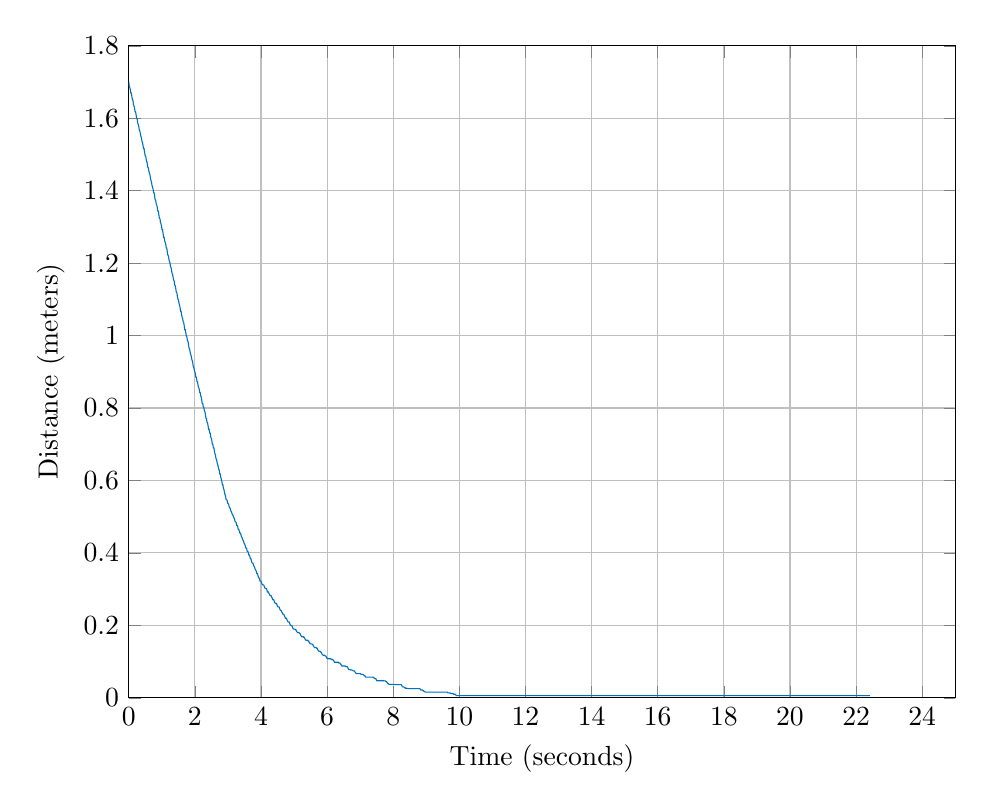
\begin{tikzpicture}

\begin{axis}[%
width=4.133in,
height=3.26in,
at={(0.693in,0.44in)},
scale only axis,
xmin=0,
xmax=25,
xmajorgrids,
xlabel={Time (seconds)},
ymin=0,
ymax=1.8,
ymajorgrids,
ylabel={Distance (meters)},
axis background/.style={fill=white}
]
\addplot [color=mycolor1,solid,forget plot]
  table[row sep=crcr]{%
0	1.70067662566856\\
0.0159490079999976	1.68893314175893\\
0.031916868999999	1.68500946445711\\
0.0480124199999981	1.67912150844895\\
0.0640135260000005	1.66931015666227\\
0.0799698209999986	1.66931014206595\\
0.0958553449999988	1.65949912144648\\
0.111901640000001	1.65165056220628\\
0.127985654999997	1.64968863564903\\
0.144012765000001	1.63794157051178\\
0.159957563999999	1.63401838731607\\
0.176058085000001	1.62813059687549\\
0.191951789000001	1.6183201782467\\
0.207983739999998	1.6183201782467\\
0.224288704999998	1.60851008775342\\
0.240120121999998	1.60066218801938\\
0.256127301999997	1.59870014222706\\
0.272139513999999	1.58694977668814\\
0.28814498	1.58302675774257\\
0.304161972999997	1.57713981112187\\
0.320125254000001	1.56733013651316\\
0.335968226999998	1.56536758301647\\
0.351865301999997	1.55752078089308\\
0.367985783999998	1.54967369972477\\
0.383978875	1.54731392614081\\
0.400055300999999	1.53673223270242\\
0.415966458000001	1.53203540052149\\
0.431809360999998	1.52614875086868\\
0.448022302999999	1.5163400180953\\
0.464088506999999	1.51634003053804\\
0.480003195	1.50653162335157\\
0.496232640999999	1.4967233663938\\
0.512145572999999	1.49632463052496\\
0.528298092999998	1.48613002803145\\
0.544302506999999	1.48104380163707\\
0.560044285999998	1.47515786888702\\
0.575953976	1.46534990548515\\
0.592025607000001	1.46338768098028\\
0.607862268999998	1.4555422414375\\
0.625949880999997	1.44769653657752\\
0.640826671	1.44533550251776\\
0.655818307	1.4355282227646\\
0.673871877	1.42809014807512\\
0.68903707	1.4241666911623\\
0.704366263	1.41435975253239\\
0.719983860999998	1.41043824334278\\
0.736120517999999	1.40455308585965\\
0.752037458999999	1.39474653115285\\
0.767990366	1.39434606064306\\
0.784070419	1.38453997361688\\
0.800173368999999	1.37513721241775\\
0.815987272	1.37317590021741\\
0.831920969999999	1.36336967452564\\
0.850269344999999	1.35944844625383\\
0.865267987999998	1.35356386374553\\
0.880145239999998	1.3437583955514\\
0.896236210000001	1.34335703644897\\
0.912138191999998	1.33355146529933\\
0.928177925999999	1.32414610631752\\
0.946818915999997	1.32218484307767\\
0.959990715	1.31237961454486\\
0.975980390999999	1.30845888138243\\
0.992136072999999	1.3025747551058\\
1.008146976	1.29236771364622\\
1.024134507	1.29236784893063\\
1.040055472	1.28217010754932\\
1.056051201	1.27119418164631\\
1.072034142	1.27119413779669\\
1.087970707	1.26138971480628\\
1.103819057	1.2574691842196\\
1.121891862	1.25158573751509\\
1.137156809	1.24137875538666\\
1.152464798	1.24137887628686\\
1.167930652	1.2307902100028\\
1.183965906	1.22216417930221\\
1.200003495	1.22020334808817\\
1.215998252	1.21039983711957\\
1.231985126	1.20451842762242\\
1.247983506	1.2005967809448\\
1.263933823	1.1903897490147\\
1.279965534	1.18842871928785\\
1.29597314	1.1801924281303\\
1.31194044	1.17117351393155\\
1.328001502	1.16921284336037\\
1.344168845	1.15941023635925\\
1.361591804	1.15352918844191\\
1.376588553	1.14960805640931\\
1.392270442	1.13940111984629\\
1.408395428	1.13744016261535\\
1.424256183	1.12880942017373\\
1.439873324	1.12018291001924\\
1.456129339	1.11822243918165\\
1.472140947	1.10842079678747\\
1.487970938	1.10057969979282\\
1.506277071	1.09821386427221\\
1.521745105	1.08841237133236\\
1.537233305	1.08449361118045\\
1.552637351	1.07782026949155\\
1.568168012	1.06723231063137\\
1.584010349	1.0672323380947\\
1.600023152	1.05743150164059\\
1.615831441	1.04959095092868\\
1.632188046	1.04722461181874\\
1.648284446	1.03742440562343\\
1.664084936	1.03546365655666\\
1.679976274	1.0264365547557\\
1.695953506	1.01624239418233\\
1.712105319	1.01624234934536\\
1.72797819	1.00644255690412\\
1.743946081	0.998602853174947\\
1.76009611	0.996235678342385\\
1.775984862	0.986436181482958\\
1.791946209	0.984476006863516\\
1.807954321	0.975446969529179\\
1.823921471	0.965252638677101\\
1.839947349	0.963292291848866\\
1.855883017	0.955453725481598\\
1.871956157	0.947614564525853\\
1.888137917	0.945247109841438\\
1.904130835	0.935448561090853\\
1.920053509	0.93153027942848\\
1.936095228	0.924457429545762\\
1.953721558	0.914263311565666\\
1.969221852	0.912302976471442\\
1.98455894	0.904465408234792\\
2.000205183	0.900138554701991\\
2.016140655	0.894258590769868\\
2.032088667	0.884460924847871\\
2.048133658	0.884461356531492\\
2.063979438	0.873865443880854\\
2.080117955	0.873071843352651\\
2.09608742	0.863274404731076\\
2.111873612	0.857396490976226\\
2.129929215	0.853477412872743\\
2.145274139	0.843270724614867\\
2.160653148	0.843270870549543\\
2.176094702	0.833473954401839\\
2.192094766	0.831113663156211\\
2.207972352	0.822479834534112\\
2.224049221	0.812285558827719\\
2.239938449	0.81228589293263\\
2.255976013	0.802489750619583\\
2.27200388	0.802079050225962\\
2.287965823	0.792283266364722\\
2.304025763	0.790323780003006\\
2.320124034	0.782487764402148\\
2.335945299	0.771890511442267\\
2.351940675	0.771093008846894\\
2.36795803	0.761297494812809\\
2.383926378	0.759338080652573\\
2.400026289	0.751091028921666\\
2.416138411	0.741295981297454\\
2.431978623	0.741296301362937\\
2.44795104	0.731501837705673\\
2.46395151	0.731099258417318\\
2.482266377	0.720104354900208\\
2.497774913	0.716185924586166\\
2.513203758	0.710309969631858\\
2.528780283	0.70010310194531\\
2.544209735	0.70010347810682\\
2.560118312	0.690309681693494\\
2.576228641	0.690309681693494\\
2.592320628	0.680112528883718\\
2.607873162	0.673833245955851\\
2.625933828	0.669115987555981\\
2.641344808	0.659322812997625\\
2.657096706	0.658909592214967\\
2.672655051	0.649116190302749\\
2.688108712	0.645198469668939\\
2.704194731	0.639323741285392\\
2.720249427	0.631083109297343\\
2.736591764	0.629126634579034\\
2.752201067	0.618128409438534\\
2.768417552	0.618128450512545\\
2.784607732	0.608336123570205\\
2.800027891	0.604004461223473\\
2.815852955	0.598129904165224\\
2.831974985	0.588337562341459\\
2.847954801	0.588338646157974\\
2.864951852	0.578141348685424\\
2.880202957	0.575376539921465\\
2.896137309	0.567141390211083\\
2.912127546	0.561265101021986\\
2.928100662	0.556934792021057\\
2.946717742	0.547143588695099\\
2.961979408	0.547143588695099\\
2.977073656	0.545185284765407\\
2.992205057	0.537352098449531\\
3.007967904	0.536945840257054\\
3.023978041	0.53302852632639\\
3.039986669	0.527154350011486\\
3.056093195	0.524791838842779\\
3.072019156	0.522027491379062\\
3.088139663	0.516153315064157\\
3.104196961	0.514195011134466\\
3.119921234	0.50986143891619\\
3.13581999	0.505946342881209\\
3.15196342	0.503988038951518\\
3.168002588	0.500069948670622\\
3.184216446	0.496154852635641\\
3.199965396	0.49419654870595\\
3.216003196	0.486363362390073\\
3.231990106	0.485957104197597\\
3.24796816	0.483998800267905\\
3.263944039	0.476165613952029\\
3.279979955	0.475761406713013\\
3.295983211	0.472997765320577\\
3.312009079	0.4651645790047\\
3.327947999	0.4651645790047\\
3.344056985	0.460831783136656\\
3.359923474	0.454957606821752\\
3.375996859	0.454957606821752\\
3.392012517	0.451040292891088\\
3.407960633	0.445166116576184\\
3.423962431	0.443207812646492\\
3.440048064	0.439289722365596\\
3.456001929	0.434968368138139\\
3.472268982	0.433010064208448\\
3.488267077	0.427135606181009\\
3.504017872	0.424369830963244\\
3.520084256	0.422009029261119\\
3.536011776	0.414175842945243\\
3.551869726	0.413760361007863\\
3.567854141	0.411802057078171\\
3.584112737	0.403968870762295\\
3.599977479	0.403968870762295\\
3.615840444	0.402010566832603\\
3.632006533	0.394177380516726\\
3.648084248	0.394177380516726\\
3.664022699	0.390260066586062\\
3.680066045	0.383979632078682\\
3.696110204	0.383979632078682\\
3.712072984	0.378105950401476\\
3.728004167	0.373381094903786\\
3.762196506	0.370606747447431\\
3.778050443	0.364730353236843\\
3.794133131	0.362771624948405\\
3.810148687	0.358856953272171\\
3.826122991	0.354938862991275\\
3.842286505	0.352980134702837\\
3.858147131	0.349065463026603\\
3.874255751	0.343188644457269\\
3.890244167	0.343188644457269\\
3.906184179	0.339273972781035\\
3.922197048	0.332990896019224\\
3.938234221	0.331034528272682\\
3.955869895	0.328672017103975\\
3.971196198	0.322392358844328\\
3.986464996	0.321989861071896\\
4.002203282	0.321574379134516\\
4.018175969	0.317659707458282\\
4.034186196	0.313741617177386\\
4.050164631	0.311782888888948\\
4.066158301	0.311782888888948\\
4.082188439	0.311782888888948\\
4.098285734	0.307868217212714\\
4.114282481	0.303950126931818\\
4.130243636	0.30199139864338\\
4.146232359	0.30199139864338\\
4.162187852	0.30199139864338\\
4.178226577	0.298076726967146\\
4.194225575	0.292199908397812\\
4.210250913	0.292199908397812\\
4.226333955	0.292199908397812\\
4.24220043	0.287878978529101\\
4.25818061	0.285919968528129\\
4.274042772	0.282002159959767\\
4.292408239	0.282002159959767\\
4.307501068	0.282002159959767\\
4.322781317	0.277683281044518\\
4.338351963	0.275724271043545\\
4.354049011	0.270988140847491\\
4.37014067	0.270585643075059\\
4.386290386	0.270585643075059\\
4.402252023	0.266670971398825\\
4.418181086	0.262752881117928\\
4.434377796	0.26079415282949\\
4.450378993	0.26079415282949\\
4.466239937	0.26079415282949\\
4.482286386	0.256879481153256\\
4.498176331	0.25296139087236\\
4.514262495	0.251002662583922\\
4.542160729	0.251002662583922\\
4.547584718	0.251002662583922\\
4.562647213	0.247087990907688\\
4.578099522	0.243169900626792\\
4.594213564	0.241211172338354\\
4.610138768	0.240804914145878\\
4.628233773	0.236890242469644\\
4.643566947	0.234931232468671\\
4.658658017	0.231013423900309\\
4.674216835	0.231013423900309\\
4.690199451	0.231013423900309\\
4.706215146	0.22669454498506\\
4.722225899	0.223917213356396\\
4.738227422	0.219596907015601\\
4.754272207	0.219596907015601\\
4.770223381	0.219596907015601\\
4.786187584	0.215682235339367\\
4.802215055	0.211764145058471\\
4.818216096	0.209805416770033\\
4.834191425	0.209805416770033\\
4.850411224	0.209805416770033\\
4.866125162	0.205890745093799\\
4.882358129	0.201972654812903\\
4.898349042	0.200013926524465\\
4.914260787	0.200013926524465\\
4.930349637	0.200013926524465\\
4.948312385	0.196099254848231\\
4.963565169	0.192181458193067\\
4.978771254	0.189817086921619\\
4.994199293	0.189817086921619\\
5.01025146	0.189817434903221\\
5.026221721	0.189818068751369\\
5.042171506	0.187859835756934\\
5.058214072	0.187859961119994\\
5.074213164	0.183945759318618\\
5.090198725	0.181986890054572\\
5.106094646	0.180028508431381\\
5.124070461	0.180029330150099\\
5.139489401	0.17962413828179\\
5.155014489	0.17962413828179\\
5.170493664	0.177666761266237\\
5.186593338	0.176847122334831\\
5.202343872	0.172932096877155\\
5.218211592	0.170569525712704\\
5.234194407	0.168611458564781\\
5.250219357	0.168611458564781\\
5.266287726	0.16861184182966\\
5.282365627	0.168612168388946\\
5.298164993	0.166654290965521\\
5.3141784	0.166654764425398\\
5.330153774	0.1627402965188\\
5.346208497	0.160781780141266\\
5.362041673	0.158824181379056\\
5.380146945	0.158824687552984\\
5.3954979	0.158824687552984\\
5.41083188	0.158825021479744\\
5.426267796	0.156867892820346\\
5.442348588	0.156868131641429\\
5.45825267	0.152953459965194\\
5.474143512	0.150996124731354\\
5.49003948	0.14903849528173\\
5.508321824	0.14903849528173\\
5.523869759	0.14903963473761\\
5.539373269	0.149039963515153\\
5.554777303	0.147082443153747\\
5.570223374	0.147083296712641\\
5.586211293	0.143169562567742\\
5.60212838	0.140801041807602\\
5.620227759	0.138843837917359\\
5.635619846	0.138844724011704\\
5.651252911	0.138844724011704\\
5.666486091	0.138845345523841\\
5.682357008	0.136888945469228\\
5.69839821	0.136888945469228\\
5.714384929	0.132974893758019\\
5.730424348	0.131018388810377\\
5.746378788	0.129060796917299\\
5.762454859	0.128651395854284\\
5.778352271	0.128652150524175\\
5.794480445	0.127828537274141\\
5.810307904	0.12587137546549\\
5.826369492	0.125463855116218\\
5.84235968899999	0.121549939669391\\
5.858078699	0.119592133539098\\
5.876516144	0.117635645348682\\
5.89172251	0.117635913480591\\
5.907126164	0.117635913480591\\
5.922522705	0.117636576643765\\
5.938456928	0.115680235276597\\
5.956202672	0.115680235276597\\
5.971638087	0.113723469669555\\
5.987015375	0.109810134147319\\
6.002236871	0.109810328608686\\
6.018288182	0.107853940898425\\
6.034197144	0.107854727900253\\
6.05020889	0.107854932195183\\
6.06612606	0.107855409175099\\
6.082226936	0.107856225640253\\
6.098194747	0.107856818538013\\
6.114170169	0.107856818538013\\
6.130209664	0.105901484115365\\
6.146224169	0.105902096667796\\
6.162199842	0.105902096667796\\
6.178198819	0.103946287707376\\
6.194193441	0.103946686118881\\
6.210289876	0.100033610080566\\
6.226225692	0.0980777328116165\\
6.242231033	0.0980787422205469\\
6.258211068	0.0980790586926743\\
6.274251377	0.0980801471465145\\
6.290201784	0.0980811763167782\\
6.306151379	0.0980815026820157\\
6.322193287	0.0980826108970561\\
6.340500172	0.0980836598286212\\
6.355438111	0.0961276283404155\\
6.371193029	0.096128309336188\\
6.386251943	0.0957140741728963\\
6.402229049	0.0937574743627649\\
6.418082311	0.0918008058968249\\
6.434184421	0.0898462636040611\\
6.450189366	0.0878906992398534\\
6.466184319	0.0878906992398534\\
6.482213684	0.0878923212869103\\
6.4982319	0.0878933618397901\\
6.514253879	0.0878933618397901\\
6.53021993	0.0878950137199321\\
6.546292846	0.0878956251345804\\
6.562224981	0.0859399969569767\\
6.578209113	0.0859410803979126\\
6.594212926	0.0859423728084514\\
6.611078946	0.08594283179216\\
6.626327829	0.083571868223991\\
6.642182253	0.0796607617266831\\
6.65804286	0.0777050087811229\\
6.674294145	0.0777054809515489\\
6.690194543	0.0777073401441053\\
6.70618737	0.0768724911347713\\
6.722188878	0.0768729733174549\\
6.738109181	0.0768737975105873\\
6.754208175	0.076459943068395\\
6.770284317	0.076459943068395\\
6.78621121	0.0745055667853922\\
6.802349172	0.0745061899092287\\
6.818325237	0.0745061899092287\\
6.834229058	0.0725513342386992\\
6.850225401	0.0705953685763969\\
6.866053503	0.0686405568338795\\
6.884206725	0.0666856324824696\\
6.899637715	0.0666866521253038\\
6.915161059	0.0666869768445091\\
6.930444435	0.0666880770620515\\
6.946153678	0.0666891168486696\\
6.962237685	0.0666891168486696\\
6.978207521	0.0666897223524467\\
6.994227561	0.0666897223524467\\
7.010238273	0.0666897223524467\\
7.026321195	0.0647349912345372\\
7.042336749	0.0647349912345372\\
7.058425589	0.0647349912345372\\
7.074217547	0.0647356902609189\\
7.090211197	0.0647356902609189\\
7.106058939	0.0627795403283751\\
7.124148022	0.0608233177315742\\
7.139596076	0.0608240268892088\\
7.154676918	0.0588681682095475\\
7.170250861	0.0569131890075338\\
7.186191661	0.0569139082964003\\
7.202309532	0.0569139082964003\\
7.218247241	0.0569139082964003\\
7.234197642	0.0569146377164762\\
7.25021322199999	0.0569146377164762\\
7.266217646	0.0569146377164762\\
7.282142423	0.0569153772677398\\
7.298176661	0.0569153772677398\\
7.314211524	0.0569153772677398\\
7.330188691	0.0569161269501683\\
7.348385527	0.0569161269501683\\
7.363634741	0.0569161269501683\\
7.378685544	0.0569168867637391\\
7.394121675	0.0569168867637391\\
7.410519626	0.0549620549751668\\
7.426411099	0.0549620549751668\\
7.442703651	0.053006676119099\\
7.458333815	0.053006676119099\\
7.474444682	0.053006676119099\\
7.490468004	0.0490955214382671\\
7.506290025	0.0471405422362536\\
7.524820306	0.0471405422362536\\
7.539909647	0.047141406358242\\
7.554970739	0.047141406358242\\
7.570178228	0.047141406358242\\
7.586399107	0.047142280670819\\
7.604778913	0.047142280670819\\
7.6180551	0.047142280670819\\
7.63430236	0.0471431651739582\\
7.650041043	0.0471431651739582\\
7.666200592	0.0471431651739582\\
7.682192859	0.047144059867632\\
7.698198025	0.047144059867632\\
7.714218675	0.047144059867632\\
7.730197096	0.0467199271973533\\
7.746051714	0.0467199271973533\\
7.764131865	0.0467199271973533\\
7.779043565	0.0447637046005525\\
7.794072642	0.0447642785895563\\
7.812166011	0.0428100388364729\\
7.827210486	0.0408541801568116\\
7.842392046	0.0388998594195549\\
7.858129678	0.0388998594195549\\
7.874058199	0.0369437094870106\\
7.892429538	0.036944378214687\\
7.907847574	0.036944378214687\\
7.923373644	0.036944378214687\\
7.938764699	0.0369450572052623\\
7.954199087	0.0369450572052623\\
7.970332112	0.0369450572052623\\
7.986261005	0.0369472535190403\\
8.00226566	0.0369479762973242\\
8.018327604	0.036529763161149\\
8.034344311	0.0365312059570495\\
8.050242554	0.0365323819252921\\
8.066189674	0.0365323819252921\\
8.082341105	0.0365323819252921\\
8.098284241	0.0365350417168069\\
8.114110887	0.0365350417168069\\
8.13019233	0.0365350417168069\\
8.146263932	0.0365377425356117\\
8.162198182	0.0365377425356117\\
8.178276894	0.0365377425356117\\
8.194249551	0.0365404843816257\\
8.210248638	0.0365404843816257\\
8.226540503	0.0365404843816257\\
8.242523729	0.0365432672547641\\
8.258258939	0.034587481537276\\
8.274224896	0.0302565251628983\\
8.290229029	0.0302587129087573\\
8.306227434	0.0302595702124331\\
8.322222794	0.0302595702124331\\
8.338224622	0.0283062317538827\\
8.354172054	0.0283076772655528\\
8.370066124	0.0263521107920357\\
8.3881145	0.0263538453086483\\
8.403276795	0.0263553114531403\\
8.41843832	0.0259357330229828\\
8.434159543	0.0259357330229828\\
8.450159512	0.0255190552273379\\
8.466222413	0.0255190552273379\\
8.482184832	0.0255190552273379\\
8.498203759	0.0255216558479514\\
8.514178762	0.0255216558479514\\
8.530298963	0.0255216558479514\\
8.546302164	0.0255242977589365\\
8.564702921	0.0255242977589365\\
8.579796061	0.0255242977589365\\
8.595012285	0.0255264030623177\\
8.611138134	0.0255269809602126\\
8.62686683	0.0255269809602126\\
8.642250797	0.0255291172310546\\
8.658317613	0.0255297054516979\\
8.674430342	0.0255297054516979\\
8.690510157	0.0255312225331876\\
8.706449844	0.0255324712333098\\
8.722200563	0.0255324712333098\\
8.738209612	0.0255330904220907\\
8.754206104	0.0255352783049645\\
8.77022715	0.0255352783049645\\
8.786203356	0.0255352783049645\\
8.80215069	0.0255381266665753\\
8.818149702	0.0235835164447664\\
8.834148323	0.0216307734461327\\
8.850282095	0.0216338125347419\\
8.86644897	0.0216338125347419\\
8.88209483	0.0216338125347419\\
8.898174503	0.0196819138301396\\
8.914372476	0.0196819138301396\\
8.930432957	0.0177271558376104\\
8.948424447	0.017729701442571\\
8.963547425	0.01577559360679\\
8.978796853	0.01577559360679\\
8.994260002	0.01577559360679\\
9.010402453	0.01577559360679\\
9.02651409	0.01577559360679\\
9.042202581	0.01577559360679\\
9.058116782	0.01577559360679\\
9.076180976	0.01577559360679\\
9.091128097	0.01577559360679\\
9.106108094	0.01577559360679\\
9.124161348	0.01577559360679\\
9.139208514	0.01577559360679\\
9.154376676	0.01577559360679\\
9.170194266	0.01577559360679\\
9.186218425	0.01577559360679\\
9.202217457	0.01577559360679\\
9.218252766	0.01577559360679\\
9.234198938	0.01577559360679\\
9.250201683	0.01577559360679\\
9.266190041	0.01577559360679\\
9.282197457	0.01577559360679\\
9.298213663	0.01577559360679\\
9.314293076	0.01577559360679\\
9.330211952	0.01577559360679\\
9.34609673	0.01577559360679\\
9.362070623	0.01577559360679\\
9.380351988	0.01577559360679\\
9.395709214	0.01577559360679\\
9.411195936	0.01577559360679\\
9.427033422	0.01577559360679\\
9.442336232	0.01577559360679\\
9.45830496	0.01577559360679\\
9.474240583	0.01577559360679\\
9.490239289	0.01577559360679\\
9.506185306	0.01577559360679\\
9.522337224	0.01577559360679\\
9.538279858	0.01577559360679\\
9.554334	0.01577559360679\\
9.570389364	0.01577559360679\\
9.586413247	0.01577559360679\\
9.60232929199999	0.01577559360679\\
9.618081989	0.01577559360679\\
9.636239221	0.01577559360679\\
9.651536924	0.0138212054876119\\
9.666989478	0.0138212054876119\\
9.682240786	0.0138212054876119\\
9.698264403	0.0138212054876119\\
9.714081305	0.0138212054876119\\
9.730211907	0.0118686890547894\\
9.746334414	0.0118686890547894\\
9.762404622	0.0118686890547894\\
9.778380126	0.0118686890547894\\
9.794337809	0.0118686890547894\\
9.810318945	0.0118686890547894\\
9.826212994	0.009914004917849\\
9.842358948	0.009914004917849\\
9.858201413	0.009914004917849\\
9.874051094	0.009914004917849\\
9.892017688	0.00795902571583529\\
9.907012727	0.00600426772330587\\
9.922472311	0.00600426772330587\\
9.938212671	0.00600426772330587\\
9.955478732	0.00600426772330587\\
9.970822958	0.00600426772330587\\
9.986386056	0.00600426772330587\\
10.002257345	0.00600426772330587\\
10.018275013	0.00600426772330587\\
10.03430931	0.00600426772330587\\
10.050151816	0.00600426772330587\\
10.066179308	0.00600426772330587\\
10.08235514	0.00600426772330587\\
10.098526661	0.00600426772330587\\
10.114615124	0.00600426772330587\\
10.130062958	0.00600426772330587\\
10.146216698	0.00600426772330587\\
10.162221092	0.00600426772330587\\
10.178232587	0.00600426772330587\\
10.194098026	0.00600426772330587\\
10.210167988	0.00600426772330587\\
10.226154487	0.00600426772330587\\
10.24221814	0.00600426772330587\\
10.258193308	0.00600426772330587\\
10.274189934	0.00600426772330587\\
10.290157866	0.00600426772330587\\
10.306198287	0.00600426772330587\\
10.322185021	0.00600426772330587\\
10.338206814	0.00600426772330587\\
10.354145955	0.00600426772330587\\
10.370056315	0.00600426772330587\\
10.386038785	0.00600426772330587\\
10.402345966	0.00600426772330587\\
10.418341434	0.00600426772330587\\
10.434315214	0.00600426772330587\\
10.450235121	0.00600426772330587\\
10.466238693	0.00600426772330587\\
10.482349759	0.00600426772330587\\
10.498212592	0.00600426772330587\\
10.516576942	0.00600426772330587\\
10.531877331	0.00600426772330587\\
10.547122781	0.00600426772330587\\
10.562388762	0.00600426772330587\\
10.578402482	0.00600426772330587\\
10.594348735	0.00600426772330587\\
10.610119663	0.00600426772330587\\
10.626055705	0.00600426772330587\\
10.644114186	0.00600426772330587\\
10.659194496	0.00600426772330587\\
10.674435607	0.00600426772330587\\
10.690199005	0.00600426772330587\\
10.706217626	0.00600426772330587\\
10.722167842	0.00600426772330587\\
10.738213555	0.00600426772330587\\
10.754320426	0.00600426772330587\\
10.770288442	0.00600426772330587\\
10.786262834	0.00600426772330587\\
10.802194313	0.00600426772330587\\
10.81838585	0.00600426772330587\\
10.834349061	0.00600426772330587\\
10.850458773	0.00600426772330587\\
10.867303394	0.00600426772330587\\
10.882221433	0.00600426772330587\\
10.898228544	0.00600426772330587\\
10.916669948	0.00600426772330587\\
10.93227971	0.00600426772330587\\
10.946677633	0.00600426772330587\\
10.962374024	0.00600426772330587\\
10.978358198	0.00600426772330587\\
10.994219162	0.00600426772330587\\
11.010198318	0.00600426772330587\\
11.026195446	0.00600426772330587\\
11.042499624	0.00600426772330587\\
11.058262568	0.00600426772330587\\
11.074349111	0.00600426772330587\\
11.090471433	0.00600426772330587\\
11.106126503	0.00600426772330587\\
11.122065204	0.00600426772330587\\
11.140209106	0.00600426772330587\\
11.155665989	0.00600426772330587\\
11.171117789	0.00600426772330587\\
11.186602793	0.00600426772330587\\
11.202251804	0.00600426772330587\\
11.218365074	0.00600426772330587\\
11.234362051	0.00600426772330587\\
11.250255655	0.00600426772330587\\
11.266355314	0.00600426772330587\\
11.282219625	0.00600426772330587\\
11.298201904	0.00600426772330587\\
11.314217228	0.00600426772330587\\
11.33021431	0.00600426772330587\\
11.346229529	0.00600426772330587\\
11.362090788	0.00600426772330587\\
11.380412392	0.00600426772330587\\
11.395814723	0.00600426772330587\\
11.411006991	0.00600426772330587\\
11.42633575	0.00600426772330587\\
11.442361089	0.00600426772330587\\
11.458253737	0.00600426772330587\\
11.474347944	0.00600426772330587\\
11.490306604	0.00600426772330587\\
11.506346093	0.00600426772330587\\
11.522321707	0.00600426772330587\\
11.538362719	0.00600426772330587\\
11.554354775	0.00600426772330587\\
11.57071091	0.00600426772330587\\
11.58633832	0.00600426772330587\\
11.602411045	0.00600426772330587\\
11.618148639	0.00600426772330587\\
11.634093954	0.00600426772330587\\
11.650066549	0.00600426772330587\\
11.666341819	0.00600426772330587\\
11.682233396	0.00600426772330587\\
11.698361802	0.00600426772330587\\
11.71432163	0.00600426772330587\\
11.730317459	0.00600426772330587\\
11.746359875	0.00600426772330587\\
11.762349014	0.00600426772330587\\
11.778410021	0.00600426772330587\\
11.79438559	0.00600426772330587\\
11.810374574	0.00600426772330587\\
11.826263327	0.00600426772330587\\
11.84238905	0.00600426772330587\\
11.858096676	0.00600426772330587\\
11.876243087	0.00600426772330587\\
11.891718308	0.00600426772330587\\
11.907252026	0.00600426772330587\\
11.922733791	0.00600426772330587\\
11.93833622	0.00600426772330587\\
11.955838837	0.00600426772330587\\
11.971061511	0.00600426772330587\\
11.986633369	0.00600426772330587\\
12.002611419	0.00600426772330587\\
12.01826099	0.00600426772330587\\
12.034419928	0.00600426772330587\\
12.050371041	0.00600426772330587\\
12.066251363	0.00600426772330587\\
12.082341849	0.00600426772330587\\
12.098320003	0.00600426772330587\\
12.11405098	0.00600426772330587\\
12.132155369	0.00600426772330587\\
12.147522359	0.00600426772330587\\
12.162986113	0.00600426772330587\\
12.17836267	0.00600426772330587\\
12.194224606	0.00600426772330587\\
12.21022927	0.00600426772330587\\
12.22619639	0.00600426772330587\\
12.242200253	0.00600426772330587\\
12.258208706	0.00600426772330587\\
12.274186826	0.00600426772330587\\
12.290188298	0.00600426772330587\\
12.306351862	0.00600426772330587\\
12.32237317	0.00600426772330587\\
12.338344123	0.00600426772330587\\
12.354301213	0.00600426772330587\\
12.370105509	0.00600426772330587\\
12.387119291	0.00600426772330587\\
12.402666806	0.00600426772330587\\
12.418426543	0.00600426772330587\\
12.434462117	0.00600426772330587\\
12.450265997	0.00600426772330587\\
12.466343614	0.00600426772330587\\
12.482375049	0.00600426772330587\\
12.498344559	0.00600426772330587\\
12.514415194	0.00600426772330587\\
12.530364116	0.00600426772330587\\
12.546246176	0.00600426772330587\\
12.562410249	0.00600426772330587\\
12.578370122	0.00600426772330587\\
12.594241406	0.00600426772330587\\
12.610104113	0.00600426772330587\\
12.626050718	0.00600426772330587\\
12.642111189	0.00600426772330587\\
12.658354266	0.00600426772330587\\
12.674343331	0.00600426772330587\\
12.690161613	0.00600426772330587\\
12.706266495	0.00600426772330587\\
12.722351135	0.00600426772330587\\
12.738363319	0.00600426772330587\\
12.754412542	0.00600426772330587\\
12.770384709	0.00600426772330587\\
12.786370701	0.00600426772330587\\
12.802319674	0.00600426772330587\\
12.818364214	0.00600426772330587\\
12.834299876	0.00600426772330587\\
12.850481709	0.00600426772330587\\
12.866053472	0.00600426772330587\\
12.884144555	0.00600426772330587\\
12.899284649	0.00600426772330587\\
12.914968482	0.00600426772330587\\
12.930484793	0.00600426772330587\\
12.948227713	0.00600426772330587\\
12.963546635	0.00600426772330587\\
12.978866156	0.00600426772330587\\
12.99431632	0.00600426772330587\\
13.010368687	0.00600426772330587\\
13.026343069	0.00600426772330587\\
13.042276522	0.00600426772330587\\
13.058256275	0.00600426772330587\\
13.074198127	0.00600426772330587\\
13.090330907	0.00600426772330587\\
13.106246191	0.00600426772330587\\
13.122036872	0.00600426772330587\\
13.140186147	0.00600426772330587\\
13.155718772	0.00600426772330587\\
13.171031986	0.00600426772330587\\
13.186413238	0.00600426772330587\\
13.202451243	0.00600426772330587\\
13.218335781	0.00600426772330587\\
13.23433384	0.00600426772330587\\
13.250355844	0.00600426772330587\\
13.266291637	0.00600426772330587\\
13.282326516	0.00600426772330587\\
13.298360026	0.00600426772330587\\
13.314225074	0.00600426772330587\\
13.330364358	0.00600426772330587\\
13.346461512	0.00600426772330587\\
13.363046732	0.00600426772330587\\
13.378053406	0.00600426772330587\\
13.394024843	0.00600426772330587\\
13.410313457	0.00600426772330587\\
13.426342157	0.00600426772330587\\
13.442321775	0.00600426772330587\\
13.458152262	0.00600426772330587\\
13.474195507	0.00600426772330587\\
13.49035821	0.00600426772330587\\
13.506207132	0.00600426772330587\\
13.522203237	0.00600426772330587\\
13.538174426	0.00600426772330587\\
13.554207104	0.00600426772330587\\
13.570205298	0.00600426772330587\\
13.586200541	0.00600426772330587\\
13.604488564	0.00600426772330587\\
13.618131877	0.00600426772330587\\
13.634153377	0.00600426772330587\\
13.650328741	0.00600426772330587\\
13.666401023	0.00600426772330587\\
13.68234818	0.00600426772330587\\
13.698314481	0.00600426772330587\\
13.714367928	0.00600426772330587\\
13.730279787	0.00600426772330587\\
13.746206851	0.00600426772330587\\
13.762173565	0.00600426772330587\\
13.778330544	0.00600426772330587\\
13.794324615	0.00600426772330587\\
13.8103362	0.00600426772330587\\
13.826340589	0.00600426772330587\\
13.84227769	0.00600426772330587\\
13.858108112	0.00600426772330587\\
13.874076863	0.00600426772330587\\
13.890369661	0.00600426772330587\\
13.90636953	0.00600426772330587\\
13.922349068	0.00600426772330587\\
13.938330871	0.00600426772330587\\
13.956076449	0.00600426772330587\\
13.971587475	0.00600426772330587\\
13.987030462	0.00600426772330587\\
14.002462725	0.00600426772330587\\
14.018402814	0.00600426772330587\\
14.034207251	0.00600426772330587\\
14.050359784	0.00600426772330587\\
14.066356591	0.00600426772330587\\
14.082216708	0.00600426772330587\\
14.098196536	0.00600426772330587\\
14.114087	0.00600426772330587\\
14.132177755	0.00600426772330587\\
14.147739496	0.00600426772330587\\
14.163094359	0.00600426772330587\\
14.178577865	0.00600426772330587\\
14.19435069	0.00600426772330587\\
14.210438868	0.00600426772330587\\
14.226365131	0.00600426772330587\\
14.242320959	0.00600426772330587\\
14.258567687	0.00600426772330587\\
14.274471764	0.00600426772330587\\
14.290335524	0.00600426772330587\\
14.306337348	0.00600426772330587\\
14.322189695	0.00600426772330587\\
14.338151775	0.00600426772330587\\
14.356417166	0.00600426772330587\\
14.370467773	0.00600426772330587\\
14.386025515	0.00600426772330587\\
14.404056078	0.00600426772330587\\
14.419229447	0.00600426772330587\\
14.434603032	0.00600426772330587\\
14.450389592	0.00600426772330587\\
14.466267334	0.00600426772330587\\
14.482388135	0.00600426772330587\\
14.498355742	0.00600426772330587\\
14.5142989	0.00600426772330587\\
14.530381654	0.00600426772330587\\
14.54641329	0.00600426772330587\\
14.56221969	0.00600426772330587\\
14.578210153	0.00600426772330587\\
14.594349071	0.00600426772330587\\
14.610313934	0.00600426772330587\\
14.626054959	0.00600426772330587\\
14.644042233	0.00600426772330587\\
14.658933717	0.00600426772330587\\
14.674391172	0.00600426772330587\\
14.690359044	0.00600426772330587\\
14.706242924	0.00600426772330587\\
14.722320484	0.00600426772330587\\
14.738421181	0.00600426772330587\\
14.754397677	0.00600426772330587\\
14.770359244	0.00600426772330587\\
14.786476574	0.00600426772330587\\
14.802240698	0.00600426772330587\\
14.818202681	0.00600426772330587\\
14.834179738	0.00600426772330587\\
14.850231389	0.00600426772330587\\
14.866126295	0.00600426772330587\\
14.882322672	0.00600426772330587\\
14.89814998	0.00600426772330587\\
14.914364372	0.00600426772330587\\
14.930331391	0.00600426772330587\\
14.948167976	0.00600426772330587\\
14.963603078	0.00600426772330587\\
14.979173922	0.00600426772330587\\
14.994602171	0.00600426772330587\\
15.010345518	0.00600426772330587\\
15.026431252	0.00600426772330587\\
15.042255973	0.00600426772330587\\
15.058259415	0.00600426772330587\\
15.074329323	0.00600426772330587\\
15.090237583	0.00600426772330587\\
15.106169753	0.00600426772330587\\
15.122084994	0.00600426772330587\\
15.140541456	0.00600426772330587\\
15.156011679	0.00600426772330587\\
15.171499031	0.00600426772330587\\
15.187086827	0.00600426772330587\\
15.202641286	0.00600426772330587\\
15.218209788	0.00600426772330587\\
15.234166781	0.00600426772330587\\
15.250357896	0.00600426772330587\\
15.266360236	0.00600426772330587\\
15.282329911	0.00600426772330587\\
15.298207197	0.00600426772330587\\
15.314188589	0.00600426772330587\\
15.330358353	0.00600426772330587\\
15.346322871	0.00600426772330587\\
15.36398955	0.00600426772330587\\
15.37887513	0.00600426772330587\\
15.394317351	0.00600426772330587\\
15.410195274	0.00600426772330587\\
15.426191233	0.00600426772330587\\
15.442206081	0.00600426772330587\\
15.458173567	0.00600426772330587\\
15.474195635	0.00600426772330587\\
15.490206153	0.00600426772330587\\
15.506186863	0.00600426772330587\\
15.522185234	0.00600426772330587\\
15.538156418	0.00600426772330587\\
15.554290105	0.00600426772330587\\
15.570329626	0.00600426772330587\\
15.58633316	0.00600426772330587\\
15.602201887	0.00600426772330587\\
15.618051239	0.00600426772330587\\
15.636170995	0.00600426772330587\\
15.651681481	0.00600426772330587\\
15.667133065	0.00600426772330587\\
15.68263171	0.00600426772330587\\
15.698365614	0.00600426772330587\\
15.714280548	0.00600426772330587\\
15.730355236	0.00600426772330587\\
15.746300196	0.00600426772330587\\
15.762193192	0.00600426772330587\\
15.778333484	0.00600426772330587\\
15.794335553	0.00600426772330587\\
15.810266376	0.00600426772330587\\
15.826327067	0.00600426772330587\\
15.842337118	0.00600426772330587\\
15.858185912	0.00600426772330587\\
15.874069968	0.00600426772330587\\
15.892707295	0.00600426772330587\\
15.908117581	0.00600426772330587\\
15.923501613	0.00600426772330587\\
15.938966353	0.00600426772330587\\
15.954115229	0.00600426772330587\\
15.970454647	0.00600426772330587\\
15.986391718	0.00600426772330587\\
16.002318867	0.00600426772330587\\
16.018219993	0.00600426772330587\\
16.034278399	0.00600426772330587\\
16.050599062	0.00600426772330587\\
16.066375337	0.00600426772330587\\
16.082351682	0.00600426772330587\\
16.098143577	0.00600426772330587\\
16.11403941	0.00600426772330587\\
16.132029672	0.00600426772330587\\
16.14684415	0.00600426772330587\\
16.162282348	0.00600426772330587\\
16.178236695	0.00600426772330587\\
16.194222878	0.00600426772330587\\
16.210240397	0.00600426772330587\\
16.226180435	0.00600426772330587\\
16.24214986	0.00600426772330587\\
16.258131688	0.00600426772330587\\
16.274195496	0.00600426772330587\\
16.290191306	0.00600426772330587\\
16.306205898	0.00600426772330587\\
16.322190687	0.00600426772330587\\
16.338237032	0.00600426772330587\\
16.354268181	0.00600426772330587\\
16.370143256	0.00600426772330587\\
16.388319311	0.00600426772330587\\
16.403668515	0.00600426772330587\\
16.419131115	0.00600426772330587\\
16.434667082	0.00600426772330587\\
16.450406318	0.00600426772330587\\
16.466250649	0.00600426772330587\\
16.482193575	0.00600426772330587\\
16.498212272	0.00600426772330587\\
16.514192645	0.00600426772330587\\
16.53040468	0.00600426772330587\\
16.54623303	0.00600426772330587\\
16.562203687	0.00600426772330587\\
16.578173232	0.00600426772330587\\
16.594340656	0.00600426772330587\\
16.610246757	0.00600426772330587\\
16.626130908	0.00600426772330587\\
16.644176584	0.00600426772330587\\
16.659216832	0.00600426772330587\\
16.674632372	0.00600426772330587\\
16.690363837	0.00600426772330587\\
16.706449851	0.00600426772330587\\
16.722348596	0.00600426772330587\\
16.738358272	0.00600426772330587\\
16.754208516	0.00600426772330587\\
16.77020599	0.00600426772330587\\
16.78616249	0.00600426772330587\\
16.80234149	0.00600426772330587\\
16.8183662	0.00600426772330587\\
16.83433569	0.00600426772330587\\
16.850215486	0.00600426772330587\\
16.866069278	0.00600426772330587\\
16.884055482	0.00600426772330587\\
16.899060478	0.00600426772330587\\
16.91418079	0.00600426772330587\\
16.930199676	0.00600426772330587\\
16.947561655	0.00600426772330587\\
16.9625954	0.00600426772330587\\
16.978355135	0.00600426772330587\\
16.994317138	0.00600426772330587\\
17.010339688	0.00600426772330587\\
17.026372241	0.00600426772330587\\
17.042402283	0.00600426772330587\\
17.058233435	0.00600426772330587\\
17.074186442	0.00600426772330587\\
17.090207428	0.00600426772330587\\
17.106309524	0.00600426772330587\\
17.122076264	0.00600426772330587\\
17.138073896	0.00600426772330587\\
17.154192326	0.00600426772330587\\
17.170253819	0.00600426772330587\\
17.186160787	0.00600426772330587\\
17.202192543	0.00600426772330587\\
17.218238737	0.00600426772330587\\
17.234319068	0.00600426772330587\\
17.250460211	0.00600426772330587\\
17.26648882	0.00600426772330587\\
17.282181042	0.00600426772330587\\
17.298180124	0.00600426772330587\\
17.314176169	0.00600426772330587\\
17.330230867	0.00600426772330587\\
17.346251049	0.00600426772330587\\
17.363930458	0.00600426772330587\\
17.378802177	0.00600426772330587\\
17.39436423	0.00600426772330587\\
17.410348223	0.00600426772330587\\
17.426442	0.00600426772330587\\
17.442395934	0.00600426772330587\\
17.4582379	0.00600426772330587\\
17.474360803	0.00600426772330587\\
17.490157817	0.00600426772330587\\
17.506141223	0.00600426772330587\\
17.522183107	0.00600426772330587\\
17.538188478	0.00600426772330587\\
17.55437952	0.00600426772330587\\
17.570420126	0.00600426772330587\\
17.586319667	0.00600426772330587\\
17.602355753	0.00600426772330587\\
17.618838337	0.00600426772330587\\
17.634046437	0.00600426772330587\\
17.650369592	0.00600426772330587\\
17.666349851	0.00600426772330587\\
17.682279063	0.00600426772330587\\
17.698330827	0.00600426772330587\\
17.714375466	0.00600426772330587\\
17.730298031	0.00600426772330587\\
17.746390799	0.00600426772330587\\
17.762392352	0.00600426772330587\\
17.778267215	0.00600426772330587\\
17.794346867	0.00600426772330587\\
17.810357214	0.00600426772330587\\
17.826202255	0.00600426772330587\\
17.84233227	0.00600426772330587\\
17.858281184	0.00600426772330587\\
17.87409669	0.00600426772330587\\
17.890192882	0.00600426772330587\\
17.906335358	0.00600426772330587\\
17.922369177	0.00600426772330587\\
17.938329866	0.00600426772330587\\
17.955880562	0.00600426772330587\\
17.97102173	0.00600426772330587\\
17.986195793	0.00600426772330587\\
18.002195336	0.00600426772330587\\
18.018197615	0.00600426772330587\\
18.034196236	0.00600426772330587\\
18.050227606	0.00600426772330587\\
18.06617032	0.00600426772330587\\
18.082194805	0.00600426772330587\\
18.098318854	0.00600426772330587\\
18.115031482	0.00600426772330587\\
18.130055926	0.00600426772330587\\
18.148272241	0.00600426772330587\\
18.163656516	0.00600426772330587\\
18.179035734	0.00600426772330587\\
18.194441111	0.00600426772330587\\
18.210321084	0.00600426772330587\\
18.226369461	0.00600426772330587\\
18.242221576	0.00600426772330587\\
18.25834519	0.00600426772330587\\
18.274398955	0.00600426772330587\\
18.290387754	0.00600426772330587\\
18.306329541	0.00600426772330587\\
18.322358821	0.00600426772330587\\
18.338336074	0.00600426772330587\\
18.354332881	0.00600426772330587\\
18.370163466	0.00600426772330587\\
18.38627158	0.00600426772330587\\
18.402346278	0.00600426772330587\\
18.41836284	0.00600426772330587\\
18.434102031	0.00600426772330587\\
18.450167701	0.00600426772330587\\
18.466321879	0.00600426772330587\\
18.482389852	0.00600426772330587\\
18.498402961	0.00600426772330587\\
18.514361636	0.00600426772330587\\
18.530371187	0.00600426772330587\\
18.546404481	0.00600426772330587\\
18.562358436	0.00600426772330587\\
18.578342479	0.00600426772330587\\
18.594275444	0.00600426772330587\\
18.610265237	0.00600426772330587\\
18.626057285	0.00600426772330587\\
18.644152132	0.00600426772330587\\
18.659662898	0.00600426772330587\\
18.67505804	0.00600426772330587\\
18.690527162	0.00600426772330587\\
18.706273048	0.00600426772330587\\
18.72238591	0.00600426772330587\\
18.738282466	0.00600426772330587\\
18.754362975	0.00600426772330587\\
18.770339365	0.00600426772330587\\
18.786354007	0.00600426772330587\\
18.802338872	0.00600426772330587\\
18.818352928	0.00600426772330587\\
18.834235957	0.00600426772330587\\
18.850214422	0.00600426772330587\\
18.866083669	0.00600426772330587\\
18.8820498	0.00600426772330587\\
18.898354537	0.00600426772330587\\
18.914411379	0.00600426772330587\\
18.930175905	0.00600426772330587\\
18.947525703	0.00600426772330587\\
18.962846903	0.00600426772330587\\
18.978792038	0.00600426772330587\\
18.994331829	0.00600426772330587\\
19.010257124	0.00600426772330587\\
19.026055592	0.00600426772330587\\
19.042163616	0.00600426772330587\\
19.058410228	0.00600426772330587\\
19.074176252	0.00600426772330587\\
19.09037677	0.00600426772330587\\
19.106385033	0.00600426772330587\\
19.122155319	0.00600426772330587\\
19.140397775	0.00600426772330587\\
19.155877481	0.00600426772330587\\
19.171419868	0.00600426772330587\\
19.186693091	0.00600426772330587\\
19.20237317	0.00600426772330587\\
19.218286393	0.00600426772330587\\
19.234203393	0.00600426772330587\\
19.250371143	0.00600426772330587\\
19.266345504	0.00600426772330587\\
19.282245772	0.00600426772330587\\
19.298191648	0.00600426772330587\\
19.314365947	0.00600426772330587\\
19.330543017	0.00600426772330587\\
19.346249206	0.00600426772330587\\
19.363514417	0.00600426772330587\\
19.37849457	0.00600426772330587\\
19.394350177	0.00600426772330587\\
19.410277561	0.00600426772330587\\
19.426308154	0.00600426772330587\\
19.442356463	0.00600426772330587\\
19.458350083	0.00600426772330587\\
19.474312927	0.00600426772330587\\
19.49037869	0.00600426772330587\\
19.506385114	0.00600426772330587\\
19.522332012	0.00600426772330587\\
19.538337073	0.00600426772330587\\
19.554242182	0.00600426772330587\\
19.570342464	0.00600426772330587\\
19.586351237	0.00600426772330587\\
19.602281451	0.00600426772330587\\
19.618172144	0.00600426772330587\\
19.634107335	0.00600426772330587\\
19.652233618	0.00600426772330587\\
19.667311989	0.00600426772330587\\
19.68239014	0.00600426772330587\\
19.698142327	0.00600426772330587\\
19.714195662	0.00600426772330587\\
19.730162997	0.00600426772330587\\
19.746158501	0.00600426772330587\\
19.762382172	0.00600426772330587\\
19.778042325	0.00600426772330587\\
19.796165944	0.00600426772330587\\
19.811016239	0.00600426772330587\\
19.826402928	0.00600426772330587\\
19.84209234	0.00600426772330587\\
19.858336482	0.00600426772330587\\
19.874130119	0.00600426772330587\\
19.890190021	0.00600426772330587\\
19.906347534	0.00600426772330587\\
19.922335531	0.00600426772330587\\
19.938363123	0.00600426772330587\\
19.956092812	0.00600426772330587\\
19.971451998	0.00600426772330587\\
19.986868144	0.00600426772330587\\
20.002291557	0.00600426772330587\\
20.018233163	0.00600426772330587\\
20.034250036	0.00600426772330587\\
20.050202537	0.00600426772330587\\
20.066208565	0.00600426772330587\\
20.082198085	0.00600426772330587\\
20.098238556	0.00600426772330587\\
20.114099991	0.00600426772330587\\
20.132161416	0.00600426772330587\\
20.147375203	0.00600426772330587\\
20.162692901	0.00600426772330587\\
20.178203757	0.00600426772330587\\
20.194207585	0.00600426772330587\\
20.210239842	0.00600426772330587\\
20.226212995	0.00600426772330587\\
20.242199699	0.00600426772330587\\
20.258210292	0.00600426772330587\\
20.274199542	0.00600426772330587\\
20.290345351	0.00600426772330587\\
20.306383802	0.00600426772330587\\
20.322349032	0.00600426772330587\\
20.338359144	0.00600426772330587\\
20.3542607	0.00600426772330587\\
20.371471601	0.00600426772330587\\
20.386383867	0.00600426772330587\\
20.402369584	0.00600426772330587\\
20.418275643	0.00600426772330587\\
20.434327462	0.00600426772330587\\
20.450709942	0.00600426772330587\\
20.466314937	0.00600426772330587\\
20.482363225	0.00600426772330587\\
20.498366562	0.00600426772330587\\
20.514289976	0.00600426772330587\\
20.530359073	0.00600426772330587\\
20.546352667	0.00600426772330587\\
20.562357412	0.00600426772330587\\
20.578372941	0.00600426772330587\\
20.594229896	0.00600426772330587\\
20.610224769	0.00600426772330587\\
20.626061738	0.00600426772330587\\
20.644302037	0.00600426772330587\\
20.659861804	0.00600426772330587\\
20.675256628	0.00600426772330587\\
20.690703408	0.00600426772330587\\
20.706732793	0.00600426772330587\\
20.722331403	0.00600426772330587\\
20.738386728	0.00600426772330587\\
20.754228002	0.00600426772330587\\
20.770213213	0.00600426772330587\\
20.786191758	0.00600426772330587\\
20.802156673	0.00600426772330587\\
20.818381942	0.00600426772330587\\
20.834364416	0.00600426772330587\\
20.850191589	0.00600426772330587\\
20.866213915	0.00600426772330587\\
20.882122914	0.00600426772330587\\
20.89834794	0.00600426772330587\\
20.914378203	0.00600426772330587\\
20.930720144	0.00600426772330587\\
20.948452596	0.00600426772330587\\
20.963959042	0.00600426772330587\\
20.979492964	0.00600426772330587\\
20.994926801	0.00600426772330587\\
21.010394474	0.00600426772330587\\
21.026344319	0.00600426772330587\\
21.042330547	0.00600426772330587\\
21.05831922	0.00600426772330587\\
21.074347789	0.00600426772330587\\
21.090314447	0.00600426772330587\\
21.106261226	0.00600426772330587\\
21.123176898	0.00600426772330587\\
21.138659149	0.00600426772330587\\
21.154336298	0.00600426772330587\\
21.170393637	0.00600426772330587\\
21.186272025	0.00600426772330587\\
21.202360645	0.00600426772330587\\
21.218398399	0.00600426772330587\\
21.234354233	0.00600426772330587\\
21.250255364	0.00600426772330587\\
21.266204838	0.00600426772330587\\
21.282203294	0.00600426772330587\\
21.298317055	0.00600426772330587\\
21.31435725	0.00600426772330587\\
21.330305808	0.00600426772330587\\
21.346348354	0.00600426772330587\\
21.363370859	0.00600426772330587\\
21.378138404	0.00600426772330587\\
21.396315081	0.00600426772330587\\
21.411680532	0.00600426772330587\\
21.427102322	0.00600426772330587\\
21.442463789	0.00600426772330587\\
21.458278594	0.00600426772330587\\
21.474331708	0.00600426772330587\\
21.490312849	0.00600426772330587\\
21.506348366	0.00600426772330587\\
21.522355018	0.00600426772330587\\
21.538294209	0.00600426772330587\\
21.554344612	0.00600426772330587\\
21.570341021	0.00600426772330587\\
21.586293269	0.00600426772330587\\
21.602403037	0.00600426772330587\\
21.618169479	0.00600426772330587\\
21.634112752	0.00600426772330587\\
21.652069688	0.00600426772330587\\
21.667556291	0.00600426772330587\\
21.683085749	0.00600426772330587\\
21.698465362	0.00600426772330587\\
21.714180356	0.00600426772330587\\
21.730352742	0.00600426772330587\\
21.746409137	0.00600426772330587\\
21.762216583	0.00600426772330587\\
21.778315688	0.00600426772330587\\
21.794373508	0.00600426772330587\\
21.810440389	0.00600426772330587\\
21.826390159	0.00600426772330587\\
21.842354372	0.00600426772330587\\
21.858422174	0.00600426772330587\\
21.874075001	0.00600426772330587\\
21.892379397	0.00600426772330587\\
21.907682511	0.00600426772330587\\
21.922826923	0.00600426772330587\\
21.938168355	0.00600426772330587\\
21.954100315	0.00600426772330587\\
21.970214783	0.00600426772330587\\
21.98635758	0.00600426772330587\\
22.002408334	0.00600426772330587\\
22.018374867	0.00600426772330587\\
22.034359296	0.00600426772330587\\
22.050368521	0.00600426772330587\\
22.066342777	0.00600426772330587\\
22.082322495	0.00600426772330587\\
22.098393159	0.00600426772330587\\
22.11411912	0.00600426772330587\\
22.132363566	0.00600426772330587\\
22.147863462	0.00600426772330587\\
22.163085698	0.00600426772330587\\
22.178193828	0.00600426772330587\\
22.194204521	0.00600426772330587\\
22.210318548	0.00600426772330587\\
22.226406411	0.00600426772330587\\
22.242242155	0.00600426772330587\\
22.258160943	0.00600426772330587\\
22.274143558	0.00600426772330587\\
22.290179583	0.00600426772330587\\
22.306362241	0.00600426772330587\\
22.322215493	0.00600426772330587\\
22.33831149	0.00600426772330587\\
22.354340219	0.00600426772330587\\
22.370776385	0.00600426772330587\\
22.393226508	0.00600426772330587\\
22.402082486	0.00600426772330587\\
22.418123712	0.00600426772330587\\
};
\end{axis}
\end{tikzpicture}%
}
      \caption{The error in displacement of the robot over time for
        $(K_{\Psi}^R, K_{\omega}^T) \equiv (0.1 K_{\Psi, max}^R, 0.2 K_{\omega, max}^T)$}
      \label{fig:19_2_distance}
    \end{figure}
  \end{minipage}
  \hfill
  \begin{minipage}{0.45\linewidth}
    \begin{figure}[H]
      \scalebox{0.6}{% This file was created by matlab2tikz.
%
%The latest updates can be retrieved from
%  http://www.mathworks.com/matlabcentral/fileexchange/22022-matlab2tikz-matlab2tikz
%where you can also make suggestions and rate matlab2tikz.
%
\definecolor{mycolor1}{rgb}{0.00000,0.44700,0.74100}%
%
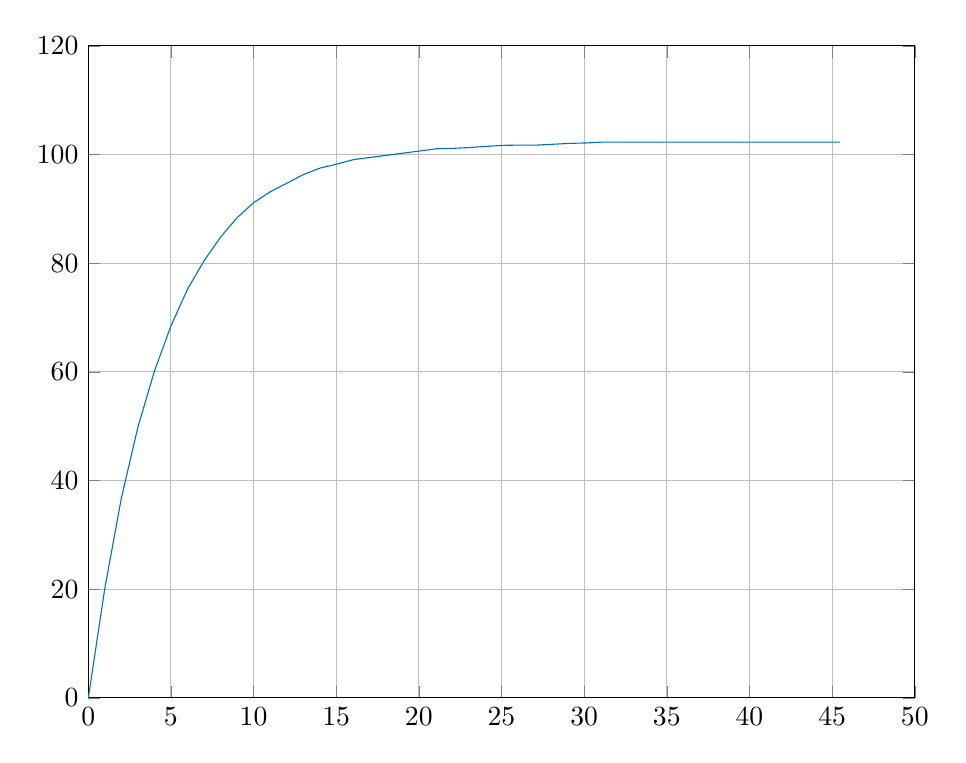
\begin{tikzpicture}

\begin{axis}[%
width=4.133in,
height=3.26in,
at={(0.693in,0.44in)},
scale only axis,
xmin=0,
xmax=50,
xmajorgrids,
ymin=0,
ymax=120,
ymajorgrids,
axis background/.style={fill=white}
]
\addplot [color=mycolor1,solid,forget plot]
  table[row sep=crcr]{%
0	0\\
0.017627004999999	0.178\\
0.0327747189999986	0.47\\
0.0477685379999988	0.792\\
0.0636867769999988	1.118\\
0.0818266279999986	1.468\\
0.0968548159999996	1.782\\
0.111926547	2.09\\
0.127790864	2.4\\
0.143747592	2.722\\
0.159650482999999	3.04\\
0.177841396	3.378\\
0.192911899999998	3.696\\
0.208020343999999	4.016\\
0.223753929	4.334\\
0.239864859999999	4.656\\
0.255788035	4.982\\
0.271866466	5.308\\
0.287787592	5.63\\
0.303792953	5.954\\
0.319799717	6.274\\
0.335788785999998	6.6\\
0.351798507999999	6.924\\
0.367796984999999	7.246\\
0.383892833999999	7.57\\
0.399726994999999	7.892\\
0.417880218999999	8.228\\
0.433032675999999	8.55\\
0.448074034	8.868\\
0.463872045	9.19\\
0.479790275999999	9.51\\
0.495954927999999	9.84\\
0.511977958999999	10.16\\
0.527804439999999	10.482\\
0.543783481999999	10.806\\
0.559864358999999	11.128\\
0.575993435999999	11.458\\
0.591895623	11.78\\
0.607806183999998	12.1\\
0.623805561999999	12.424\\
0.639878685999999	12.744\\
0.655862683999998	13.07\\
0.671809347999999	13.394\\
0.688007375	13.718\\
0.703977030999999	14.04\\
0.719817071999999	14.376\\
0.735789037999999	14.694\\
0.751903521	15.012\\
0.767862266999999	15.336\\
0.78380684	15.656\\
0.799775462999999	15.98\\
0.81574808	16.302\\
0.831793863	16.628\\
0.847800606999999	16.948\\
0.863872895	17.272\\
0.879949246999999	17.61\\
0.896461672999998	17.938\\
0.911939472999999	18.252\\
0.928073790999999	18.574\\
0.944029895	18.89\\
0.959984832999999	19.216\\
0.976055911999999	19.538\\
0.992033660999998	19.864\\
1.012990514	20.23\\
1.025009675	20.48\\
1.040490137	20.728\\
1.055992294	21.004\\
1.071960656	21.266\\
1.088198667	21.522\\
1.104155596	21.794\\
1.11988478	22.054\\
1.13593575	22.312\\
1.151771797	22.578\\
1.167630294	22.836\\
1.185782897	23.108\\
1.201377082	23.386\\
1.216831846	23.646\\
1.232294868	23.908\\
1.248046299	24.166\\
1.263878221	24.43\\
1.279828496	24.692\\
1.295736922	24.958\\
1.311727252	25.22\\
1.327788756	25.488\\
1.343763182	25.754\\
1.359802976	26.028\\
1.375801552	26.29\\
1.39177865	26.554\\
1.407700529	26.816\\
1.423930848	27.08\\
1.440279624	27.352\\
1.456002694	27.614\\
1.471926449	27.874\\
1.488010619	28.14\\
1.503817976	28.404\\
1.519900482	28.668\\
1.535805181	28.932\\
1.552002246	29.196\\
1.56821883	29.472\\
1.583995539	29.738\\
1.599878204	30.01\\
1.615790014	30.264\\
1.631877599	30.53\\
1.647664555	30.788\\
1.665701588	31.064\\
1.680928124	31.326\\
1.696404631	31.59\\
1.71186283	31.852\\
1.730252207	32.126\\
1.745645141	32.402\\
1.761083347	32.658\\
1.776474597	32.918\\
1.79196574	33.182\\
1.807868222	33.442\\
1.823795551	33.708\\
1.839802816	33.972\\
1.855789395	34.236\\
1.871808517	34.508\\
1.887929471	34.772\\
1.903865954	35.048\\
1.919657486	35.306\\
1.935961966	35.566\\
1.952033898	35.84\\
1.968023889	36.112\\
1.983856769	36.37\\
1.999759955	36.628\\
2.015796794	36.876\\
2.031812557	37.092\\
2.047764207	37.292\\
2.063752644	37.49\\
2.079965696	37.694\\
2.095818827	37.902\\
2.112126193	38.114\\
2.127809033	38.33\\
2.143827403	38.534\\
2.15982371	38.742\\
2.175876498	38.954\\
2.191776335	39.162\\
2.207786788	39.372\\
2.22386105	39.58\\
2.239829167	39.792\\
2.255861534	40.002\\
2.271812918	40.208\\
2.287824834	40.416\\
2.303867951	40.628\\
2.319808069	40.836\\
2.335757003	41.046\\
2.351769706	41.252\\
2.367820199	41.464\\
2.383719034	41.672\\
2.399745996	41.882\\
2.415802099	42.1\\
2.431804415	42.308\\
2.447744153	42.512\\
2.463769394	42.722\\
2.479741956	42.93\\
2.495743564	43.138\\
2.511940698	43.348\\
2.527858325	43.558\\
2.543976016	43.768\\
2.559815597	43.974\\
2.575868305	44.184\\
2.591871847	44.394\\
2.608070682	44.602\\
2.624005909	44.814\\
2.640049349	45.022\\
2.655665488	45.232\\
2.673942147	45.454\\
2.689472021	45.664\\
2.704838134	45.868\\
2.720318682	46.074\\
2.735801307	46.28\\
2.751804645	46.486\\
2.767919825	46.71\\
2.783806552	46.916\\
2.799954908	47.12\\
2.815892515	47.328\\
2.831927218	47.534\\
2.847739999	47.742\\
2.864243923	47.952\\
2.879977955	48.172\\
2.895694244	48.378\\
2.911711427	48.584\\
2.927872543	48.792\\
2.943880107	49\\
2.960152786	49.208\\
2.976136849	49.418\\
2.992442385	49.63\\
3.010645236	49.852\\
3.024073413	50.016\\
3.039995715	50.17\\
3.055957568	50.328\\
3.071891633	50.492\\
3.088032265	50.662\\
3.103986055	50.826\\
3.119999544	50.992\\
3.135817002	51.154\\
3.151656771	51.316\\
3.169655073	51.49\\
3.184560306	51.65\\
3.199850563	51.812\\
3.216011025	51.986\\
3.232002044	52.148\\
3.247731998	52.31\\
3.263960171	52.472\\
3.279937487	52.638\\
3.29590332	52.8\\
3.311825067	52.966\\
3.328017257	53.132\\
3.343986025	53.296\\
3.359980577	53.462\\
3.375999619	53.626\\
3.391820693	53.79\\
3.407689629	53.956\\
3.42366058	54.12\\
3.440004937	54.292\\
3.456107988	54.458\\
3.471868399	54.618\\
3.487793105	54.782\\
3.503883728	54.948\\
3.519863356	55.116\\
3.535815948	55.278\\
3.551801023	55.442\\
3.567816813	55.604\\
3.583756631	55.77\\
3.600207591	55.934\\
3.616034661	56.11\\
3.631973083	56.268\\
3.647802512	56.434\\
3.663665581	56.594\\
3.679625737	56.768\\
3.695994628	56.928\\
3.711881169	57.092\\
3.727860845	57.256\\
3.743966872	57.42\\
3.760035076	57.582\\
3.775954432	57.754\\
3.794297178	57.924\\
3.809654195	58.094\\
3.82476268	58.252\\
3.839869516	58.412\\
3.855807023	58.576\\
3.871868883	58.738\\
3.888104941	58.906\\
3.903784654	59.068\\
3.919657818	59.234\\
3.937701482	59.406\\
3.95291856	59.566\\
3.968301958	59.73\\
3.983983911	59.892\\
3.999825184	60.056\\
4.017519282	60.228\\
4.032710384	60.35\\
4.047866862	60.478\\
4.064139198	60.612\\
4.080029619	60.752\\
4.095882935	60.886\\
4.111873057	61.014\\
4.128136433	61.144\\
4.143892278	61.274\\
4.159739011	61.404\\
4.177935996	61.544\\
4.193345052	61.678\\
4.208641668	61.806\\
4.224113879	61.938\\
4.239947172	62.08\\
4.25597298	62.21\\
4.271930102	62.342\\
4.287987125	62.474\\
4.303951243	62.604\\
4.319947318	62.738\\
4.33594442	62.874\\
4.351974207	63.004\\
4.367976556	63.142\\
4.384053314	63.278\\
4.399827501	63.408\\
4.416341439	63.538\\
4.43181896	63.674\\
4.447804054	63.804\\
4.463974977	63.936\\
4.479937368	64.07\\
4.495878271	64.204\\
4.512020782	64.336\\
4.527884096	64.472\\
4.543892205	64.604\\
4.560117343	64.738\\
4.575878175	64.87\\
4.591862339	65.004\\
4.60795167	65.136\\
4.623975423	65.268\\
4.63998543	65.404\\
4.655723423	65.536\\
4.671695315	65.672\\
4.687811757	65.812\\
4.703935277	65.94\\
4.719812847	66.072\\
4.736035157	66.202\\
4.751879723	66.334\\
4.76798453	66.468\\
4.783822211	66.6\\
4.799956619	66.74\\
4.816068272	66.87\\
4.832021379	67.002\\
4.847904669	67.136\\
4.863997323	67.268\\
4.880132879	67.4\\
4.895649057	67.534\\
4.913762656	67.67\\
4.928748145	67.804\\
4.943924162	67.936\\
4.959808103	68.066\\
4.975789906	68.198\\
4.99176524	68.334\\
5.009068286	68.476\\
5.024370002	68.58\\
5.039933467	68.682\\
5.055988474	68.786\\
5.071998062	68.902\\
5.087819251	69.01\\
5.103805213	69.114\\
5.119851335	69.218\\
5.135966847	69.326\\
5.151649607	69.434\\
5.16764885	69.54\\
5.185692803	69.654\\
5.201113096	69.76\\
5.216486093	69.866\\
5.231982492	69.972\\
5.247898811	70.082\\
5.263797546	70.188\\
5.27980209	70.296\\
5.295776747	70.406\\
5.31182054	70.51\\
5.327991732	70.618\\
5.343874794	70.726\\
5.359873114	70.836\\
5.37587304	70.944\\
5.391872199	71.05\\
5.407690814	71.16\\
5.423662849	71.27\\
5.43987021	71.376\\
5.455733015	71.48\\
5.471794601	71.594\\
5.487823922	71.7\\
5.503824307	71.812\\
5.51982593	71.916\\
5.535817074	72.022\\
5.551801493	72.13\\
5.567802253	72.24\\
5.583915624	72.35\\
5.599790274	72.454\\
5.615828665	72.564\\
5.631818301	72.67\\
5.647945694	72.778\\
5.663646814	72.884\\
5.679891156	72.99\\
5.695861745	73.1\\
5.711814472	73.206\\
5.727862319	73.316\\
5.743821266	73.42\\
5.759807609	73.53\\
5.775791551	73.642\\
5.791800621	73.748\\
5.807805982	73.856\\
5.823799376	73.96\\
5.839791256	74.07\\
5.855824616	74.176\\
5.871799659	74.288\\
5.887755623	74.394\\
5.903704049	74.502\\
5.921724081	74.614\\
5.936761629	74.718\\
5.951810318	74.824\\
5.967852728	74.93\\
5.98379203	75.04\\
5.999801205	75.146\\
6.017264463	75.258\\
6.032409405	75.338\\
6.047793604	75.416\\
6.06381671	75.498\\
6.079849469	75.582\\
6.095790399	75.662\\
6.111870364	75.75\\
6.127954634	75.832\\
6.143857899	75.916\\
6.159676503	76\\
6.178057595	76.086\\
6.193509908	76.172\\
6.208640332	76.25\\
6.223923328	76.332\\
6.239998472	76.422\\
6.255798688	76.504\\
6.271888646	76.586\\
6.287788683	76.668\\
6.303821487	76.752\\
6.319868678	76.834\\
6.335758226	76.92\\
6.351808204	77.002\\
6.367935712	77.086\\
6.383771678	77.17\\
6.399881913	77.256\\
6.415683113	77.338\\
6.433990748	77.426\\
6.449409285	77.508\\
6.464666952	77.59\\
6.480081064	77.676\\
6.495982991	77.758\\
6.511820096	77.844\\
6.52779437	77.922\\
6.561458611	78.026\\
6.566951054	78.098\\
6.575775965	78.176\\
6.591698844	78.256\\
6.609903056	78.346\\
6.625018457	78.428\\
6.640392152	78.512\\
6.655669563	78.596\\
6.673841178	78.682\\
6.688906606	78.764\\
6.704260517	78.85\\
6.719812025	78.932\\
6.735893719	79.014\\
6.751819076	79.094\\
6.767860517	79.18\\
6.783908014	79.266\\
6.7997936	79.35\\
6.815864408	79.432\\
6.831863485	79.516\\
6.847906865	79.6\\
6.863861132	79.682\\
6.879676884	79.768\\
6.896006415	79.852\\
6.911657869	79.938\\
6.927860502	80.018\\
6.94369346	80.1\\
6.959823531	80.184\\
6.9758632	80.27\\
6.991885189	80.352\\
7.00948517	80.444\\
7.024426289	80.512\\
7.039677298	80.578\\
7.055689692	80.644\\
7.071722285	80.722\\
7.087716341	80.79\\
7.103810163	80.858\\
7.119807335	80.924\\
7.135860429	80.992\\
7.151679383	81.062\\
7.167643742	81.134\\
7.185934224	81.206\\
7.201095538	81.274\\
7.21640644	81.346\\
7.231757846	81.416\\
7.247865384	81.484\\
7.263864143	81.552\\
7.279708539	81.622\\
7.295882535	81.692\\
7.311827324	81.762\\
7.327747191	81.832\\
7.343857996	81.902\\
7.35978732	81.972\\
7.375788366	82.042\\
7.391945321	82.11\\
7.407687765	82.18\\
7.425965365	82.252\\
7.441202461	82.322\\
7.45642996	82.394\\
7.471824818	82.46\\
7.487877432	82.53\\
7.503882822	82.6\\
7.519744581	82.668\\
7.535691337	82.738\\
7.551893524	82.808\\
7.567887389	82.882\\
7.583888606	82.95\\
7.599816401	83.02\\
7.615863282	83.09\\
7.631853937	83.156\\
7.647931993	83.226\\
7.66549047	83.298\\
7.680518346	83.366\\
7.69611649	83.436\\
7.711876591	83.506\\
7.72787203	83.576\\
7.743948931	83.648\\
7.759749242	83.718\\
7.775828293	83.784\\
7.791858556	83.856\\
7.80771977	83.924\\
7.823765762	83.992\\
7.839742714	84.062\\
7.855719797	84.132\\
7.87172126	84.202\\
7.887887059	84.274\\
7.90375023	84.342\\
7.919874387	84.412\\
7.935851307	84.482\\
7.951780743	84.552\\
7.967936338	84.622\\
7.983877699	84.692\\
7.999872474	84.762\\
8.017289673	84.832\\
8.032245091	84.89\\
8.04763903	84.94\\
8.065696498	84.998\\
8.080668024	85.056\\
8.095876252	85.114\\
8.111870934	85.17\\
8.127870181	85.226\\
8.143972467	85.282\\
8.159678654	85.34\\
8.177706287	85.396\\
8.192922015	85.456\\
8.208198169	85.51\\
8.223801299	85.57\\
8.239818151	85.624\\
8.255660558	85.68\\
8.274159738	85.742\\
8.289633987	85.796\\
8.305104366	85.854\\
8.320541299	85.91\\
8.335964807	85.968\\
8.351868499	86.022\\
8.367887245	86.084\\
8.383698391	86.14\\
8.399640567	86.198\\
8.417764893	86.252\\
8.433303919	86.312\\
8.448830031	86.368\\
8.464404805	86.424\\
8.479893582	86.48\\
8.495911026	86.538\\
8.511791925	86.594\\
8.527852687	86.65\\
8.543787388	86.71\\
8.559786545	86.764\\
8.575815365	86.822\\
8.591805957	86.88\\
8.607862249	86.94\\
8.623720291	86.994\\
8.639911007	87.054\\
8.655672235	87.112\\
8.671764948	87.166\\
8.687892562	87.224\\
8.703952626	87.28\\
8.719695361	87.338\\
8.735950867	87.394\\
8.751786448	87.45\\
8.767853239	87.508\\
8.783810831	87.564\\
8.799793356	87.622\\
8.815821188	87.68\\
8.83178271	87.736\\
8.847822609	87.792\\
8.863706475	87.85\\
8.879804456	87.912\\
8.895902557	87.964\\
8.911782706	88.024\\
8.927698842	88.08\\
8.943768055	88.136\\
8.959796879	88.192\\
8.975795059	88.25\\
8.991776516	88.306\\
9.009183798	88.37\\
9.024356738	88.414\\
9.039791547	88.454\\
9.055750553	88.496\\
9.071819048	88.54\\
9.087806298	88.584\\
9.103760237	88.63\\
9.119860534	88.676\\
9.135748083	88.722\\
9.151731427	88.762\\
9.16764455	88.808\\
9.1837989	88.852\\
9.199793517	88.896\\
9.21593639	88.942\\
9.23182003	88.984\\
9.2479285	89.03\\
9.263788822	89.072\\
9.279958025	89.12\\
9.295662011	89.164\\
9.311772648	89.208\\
9.327785396	89.252\\
9.343896953	89.296\\
9.36174587	89.34\\
9.37686792	89.386\\
9.391936599	89.43\\
9.407782895	89.472\\
9.423824204	89.516\\
9.439745033	89.562\\
9.455852901	89.606\\
9.471818392	89.652\\
9.487779052	89.694\\
9.503896442	89.74\\
9.519679327	89.784\\
9.537731842	89.828\\
9.552990903	89.872\\
9.568209512	89.918\\
9.583787635	89.962\\
9.599762262	90.006\\
9.615849664	90.054\\
9.631664779	90.094\\
9.647854574	90.14\\
9.663722671	90.184\\
9.679672128	90.226\\
9.695786852	90.272\\
9.711790344	90.316\\
9.727860316	90.362\\
9.743805837	90.404\\
9.759822954	90.45\\
9.775941206	90.494\\
9.79177988	90.54\\
9.807783946	90.582\\
9.823803923	90.626\\
9.839762147	90.672\\
9.855791197	90.716\\
9.871864011	90.762\\
9.887853005	90.806\\
9.90364736	90.852\\
9.921648706	90.896\\
9.936677319	90.94\\
9.951642233	90.982\\
9.967677502	91.026\\
9.983782489	91.072\\
9.999776034	91.116\\
10.017032729	91.156\\
10.031978272	91.188\\
10.047690637	91.218\\
10.06577541	91.25\\
10.080814346	91.284\\
10.095871258	91.316\\
10.111786771	91.348\\
10.127786199	91.378\\
10.143779097	91.408\\
10.159640141	91.44\\
10.177696212	91.472\\
10.192853838	91.504\\
10.208131443	91.536\\
10.223802675	91.568\\
10.239674315	91.598\\
10.25586475	91.632\\
10.271851904	91.664\\
10.287802486	91.696\\
10.303807967	91.726\\
10.319863643	91.756\\
10.335894036	91.786\\
10.35167594	91.818\\
10.367813817	91.852\\
10.383893406	91.886\\
10.399952478	91.916\\
10.415702439	91.946\\
10.431788034	91.976\\
10.447799307	92.01\\
10.463866425	92.042\\
10.479969056	92.076\\
10.495809869	92.106\\
10.511784245	92.136\\
10.527786086	92.168\\
10.543734214	92.2\\
10.560073714	92.234\\
10.575998573	92.266\\
10.591904163	92.298\\
10.607980956	92.328\\
10.623763951	92.358\\
10.639788313	92.392\\
10.655690043	92.424\\
10.673977748	92.456\\
10.689360587	92.488\\
10.704531717	92.518\\
10.719792021	92.55\\
10.735798239	92.582\\
10.75186553	92.614\\
10.767775791	92.648\\
10.783775264	92.678\\
10.799749044	92.708\\
10.815782855	92.738\\
10.831717566	92.772\\
10.847758733	92.806\\
10.863861364	92.838\\
10.879660949	92.868\\
10.895823336	92.898\\
10.911650793	92.93\\
10.92980154	92.964\\
10.945560424	92.996\\
10.961214712	93.026\\
10.976697902	93.056\\
10.992021073	93.088\\
11.009933884	93.124\\
11.025040045	93.148\\
11.040313713	93.174\\
11.055786283	93.196\\
11.071773382	93.224\\
11.087742231	93.248\\
11.103751972	93.274\\
11.11972356	93.298\\
11.135746382	93.326\\
11.151727239	93.35\\
11.167700504	93.376\\
11.183758031	93.398\\
11.199829557	93.426\\
11.216047419	93.448\\
11.232014524	93.476\\
11.247744406	93.498\\
11.263763681	93.526\\
11.27981097	93.552\\
11.29579802	93.576\\
11.311791158	93.604\\
11.327771552	93.626\\
11.343754788	93.654\\
11.359972802	93.678\\
11.375888118	93.706\\
11.392157899	93.728\\
11.407860489	93.756\\
11.42365893	93.778\\
11.441916249	93.806\\
11.457588499	93.83\\
11.473253783	93.856\\
11.488803536	93.886\\
11.504431502	93.906\\
11.519934064	93.934\\
11.536288165	93.956\\
11.551979189	93.984\\
11.567796525	94.006\\
11.583773792	94.036\\
11.599772218	94.058\\
11.615850008	94.086\\
11.631792206	94.11\\
11.647954717	94.136\\
11.663663578	94.16\\
11.681747497	94.186\\
11.697206305	94.214\\
11.712599745	94.236\\
11.728058099	94.266\\
11.743995995	94.286\\
11.759795626	94.316\\
11.775782826	94.336\\
11.791787054	94.366\\
11.807740087	94.388\\
11.82377295	94.416\\
11.83976647	94.438\\
11.855942387	94.466\\
11.871882731	94.488\\
11.887826409	94.516\\
11.903721295	94.538\\
11.922163025	94.566\\
11.937720696	94.594\\
11.953041426	94.616\\
11.968370636	94.644\\
11.983893938	94.668\\
11.999905004	94.694\\
12.017284458	94.722\\
12.032417538	94.746\\
12.047797457	94.77\\
12.063989406	94.796\\
12.079796247	94.82\\
12.095686649	94.846\\
12.112067325	94.87\\
12.127865446	94.896\\
12.143816259	94.922\\
12.159651027	94.946\\
12.177698274	94.974\\
12.192953867	94.996\\
12.208369859	95.024\\
12.223922395	95.046\\
12.239957659	95.076\\
12.255889102	95.098\\
12.271873441	95.126\\
12.287864675	95.148\\
12.30380106	95.176\\
12.319820087	95.198\\
12.336503449	95.226\\
12.351913397	95.252\\
12.367694297	95.276\\
12.383798895	95.304\\
12.399808599	95.326\\
12.415688548	95.354\\
12.43188638	95.376\\
12.44774749	95.404\\
12.463642034	95.428\\
12.479716257	95.458\\
12.495730589	95.478\\
12.511766939	95.506\\
12.527956128	95.528\\
12.543955981	95.556\\
12.559794459	95.582\\
12.575722483	95.606\\
12.592062439	95.634\\
12.607760823	95.656\\
12.623762671	95.684\\
12.639766226	95.706\\
12.655875988	95.736\\
12.671647968	95.758\\
12.689894019	95.786\\
12.705433091	95.81\\
12.721022436	95.836\\
12.736595895	95.86\\
12.751984769	95.886\\
12.768229963	95.912\\
12.784077096	95.936\\
12.800274607	95.964\\
12.815902278	95.986\\
12.831804952	96.014\\
12.847796557	96.036\\
12.863970004	96.064\\
12.885462958	96.09\\
12.897481368	96.116\\
12.912772037	96.142\\
12.928278493	96.166\\
12.943775676	96.188\\
12.959911936	96.216\\
12.975750846	96.238\\
12.991781669	96.266\\
13.01254802	96.296\\
13.024416124	96.308\\
13.039827555	96.328\\
13.055822899	96.348\\
13.071781674	96.368\\
13.09010038	96.388\\
13.10511796	96.406\\
13.120279834	96.426\\
13.135774828	96.446\\
13.151665986	96.462\\
13.169703295	96.48\\
13.184865433	96.498\\
13.200007553	96.52\\
13.216155553	96.538\\
13.231799509	96.558\\
13.247914334	96.578\\
13.2637422	96.596\\
13.2797809	96.616\\
13.295781454	96.636\\
13.314162745	96.654\\
13.329294355	96.67\\
13.344380055	96.688\\
13.359871988	96.708\\
13.375699269	96.728\\
13.391810906	96.748\\
13.40772616	96.768\\
13.423987777	96.788\\
13.439753987	96.806\\
13.455884569	96.826\\
13.471795957	96.844\\
13.487891437	96.862\\
13.503819744	96.88\\
13.519933562	96.9\\
13.5358178	96.918\\
13.551805945	96.938\\
13.567884657	96.958\\
13.583927984	96.978\\
13.599823909	96.996\\
13.615738683	97.016\\
13.631861933	97.036\\
13.647887573	97.05\\
13.663681336	97.068\\
13.679678923	97.088\\
13.697775157	97.108\\
13.712993406	97.128\\
13.72813961	97.148\\
13.74389068	97.168\\
13.759725303	97.186\\
13.775867666	97.206\\
13.79185465	97.226\\
13.807805794	97.242\\
13.823863228	97.258\\
13.84001179	97.278\\
13.855669229	97.298\\
13.871820539	97.318\\
13.887863199	97.338\\
13.903926136	97.358\\
13.919693996	97.376\\
13.935866018	97.396\\
13.951712619	97.416\\
13.967859033	97.432\\
13.983821544	97.45\\
13.99998371	97.468\\
14.017401031	97.488\\
14.032850492	97.498\\
14.048055229	97.512\\
14.06389067	97.528\\
14.079861388	97.538\\
14.095806004	97.548\\
14.111874146	97.562\\
14.127864332	97.578\\
14.143658792	97.588\\
14.161737314	97.598\\
14.176606747	97.614\\
14.191639854	97.628\\
14.209825548	97.638\\
14.225007175	97.65\\
14.240200642	97.668\\
14.255777753	97.678\\
14.271952699	97.688\\
14.287703853	97.702\\
14.303878313	97.718\\
14.319879389	97.728\\
14.335796235	97.738\\
14.351780679	97.752\\
14.367769638	97.768\\
14.383812038	97.778\\
14.400056211	97.788\\
14.415679017	97.804\\
14.431652417	97.818\\
14.447810581	97.828\\
14.549835343	97.854\\
14.567883932	97.872\\
14.583028783	97.882\\
14.598227052	97.892\\
14.613992099	97.906\\
14.630003103	97.922\\
14.64597791	97.932\\
14.66197217	97.942\\
14.67782766	97.956\\
14.695988156	97.972\\
14.711244948	97.982\\
14.72647896	97.994\\
14.742313078	98.008\\
14.758250536	98.022\\
14.774059151	98.032\\
14.790003113	98.046\\
14.806165585	98.06\\
14.822019563	98.072\\
14.838105371	98.082\\
14.854005462	98.096\\
14.870046942	98.112\\
14.88605715	98.122\\
14.901879986	98.134\\
14.920148164	98.15\\
14.935448993	98.162\\
14.950779369	98.172\\
14.966098463	98.186\\
14.981994657	98.2\\
14.998048222	98.212\\
15.015722995	98.222\\
15.030955506	98.236\\
15.0461657	98.252\\
15.062008338	98.262\\
15.077963245	98.272\\
15.093960327	98.288\\
15.110067945	98.302\\
15.125987216	98.312\\
15.142027732	98.324\\
15.158057018	98.338\\
15.173976915	98.352\\
15.189969592	98.362\\
15.205974628	98.376\\
15.222033721	98.39\\
15.237839046	98.402\\
15.254080174	98.412\\
15.270029809	98.426\\
15.285944329	98.442\\
15.302009686	98.452\\
15.317968277	98.462\\
15.334083923	98.476\\
15.350038875	98.492\\
15.365915945	98.502\\
15.381981483	98.514\\
15.397930691	98.53\\
15.413814783	98.542\\
15.430014931	98.552\\
15.445987703	98.566\\
15.462046406	98.58\\
15.478054524	98.592\\
15.493962092	98.602\\
15.509984066	98.616\\
15.525987688	98.632\\
15.541971942	98.642\\
15.558014342	98.654\\
15.574018189	98.666\\
15.589902778	98.682\\
15.605971161	98.692\\
15.622028971	98.704\\
15.637985306	98.72\\
15.654193321	98.732\\
15.670030446	98.744\\
15.686000978	98.756\\
15.701995415	98.77\\
15.718020516	98.782\\
15.733943751	98.792\\
15.749943845	98.808\\
15.765963985	98.822\\
15.782092279	98.832\\
15.797959375	98.842\\
15.813988718	98.856\\
15.830073479	98.872\\
15.845985884	98.882\\
15.861895561	98.896\\
15.877974462	98.91\\
15.893959627	98.922\\
15.909872714	98.932\\
15.926041223	98.946\\
15.941945081	98.962\\
15.957984585	98.972\\
15.974038701	98.984\\
15.989988527	98.996\\
16.008685309	99.012\\
16.023937795	99.02\\
16.039299975	99.03\\
16.054581055	99.046\\
16.06997232	99.056\\
16.086109109	99.066\\
16.102019645	99.074\\
16.117919021	99.084\\
16.13403094	99.092\\
16.150088263	99.094\\
16.165937074	99.104\\
16.184047898	99.108\\
16.199447043	99.114\\
16.214637436	99.122\\
16.230096627	99.124\\
16.246064263	99.134\\
16.262199208	99.142\\
16.277968704	99.144\\
16.293963256	99.154\\
16.309968832	99.16\\
16.325961746	99.164\\
16.341966906	99.174\\
16.357952483	99.174\\
16.373974752	99.184\\
16.390075409	99.192\\
16.405939167	99.194\\
16.421937901	99.204\\
16.437899418	99.21\\
16.453866954	99.214\\
16.469993829	99.224\\
16.485997918	99.23\\
16.501991823	99.234\\
16.51799338	99.244\\
16.533955448	99.244\\
16.549906676	99.254\\
16.566134217	99.262\\
16.582160875	99.264\\
16.598096614	99.274\\
16.613988193	99.28\\
16.630037323	99.284\\
16.645985074	99.294\\
16.661840539	99.296\\
16.679970289	99.304\\
16.695042607	99.314\\
16.710292201	99.314\\
16.725973232	99.324\\
16.74209833	99.332\\
16.757955906	99.334\\
16.774004881	99.344\\
16.79017237	99.35\\
16.80613542	99.354\\
16.822120615	99.364\\
16.837949952	99.366\\
16.854034348	99.374\\
16.870082266	99.384\\
16.886018279	99.384\\
16.902144429	99.394\\
16.918020177	99.402\\
16.933977524	99.404\\
16.950000057	99.414\\
16.965987094	99.42\\
16.981977885	99.424\\
16.998000683	99.434\\
17.015391868	99.436\\
17.030454143	99.444\\
17.04596982	99.452\\
17.061964066	99.454\\
17.077945328	99.464\\
17.09398425	99.474\\
17.109964299	99.474\\
17.126004023	99.484\\
17.142068874	99.49\\
17.158040293	99.494\\
17.17403095	99.504\\
17.190065513	99.504\\
17.206143514	99.514\\
17.222087416	99.522\\
17.238095799	99.524\\
17.254090716	99.534\\
17.270008459	99.54\\
17.28611973	99.544\\
17.302142566	99.554\\
17.318139678	99.556\\
17.334151163	99.564\\
17.350127293	99.574\\
17.365938525	99.574\\
17.381904401	99.584\\
17.400379986	99.592\\
17.415299264	99.594\\
17.430387247	99.604\\
17.446147817	99.61\\
17.462092222	99.614\\
17.4782019	99.624\\
17.493970848	99.626\\
17.50986969	99.634\\
17.526107337	99.642\\
17.541999823	99.644\\
17.557967356	99.654\\
17.574030976	99.662\\
17.590012639	99.664\\
17.605950663	99.674\\
17.621969539	99.68\\
17.637941219	99.684\\
17.654074415	99.694\\
17.6698351	99.696\\
17.687979974	99.704\\
17.703261456	99.712\\
17.718304107	99.714\\
17.733927875	99.724\\
17.749959904	99.73\\
17.765940179	99.734\\
17.781924097	99.744\\
17.797913652	99.746\\
17.814003249	99.754\\
17.829902438	99.764\\
17.846086212	99.764\\
17.862094533	99.774\\
17.878132252	99.782\\
17.894149801	99.784\\
17.909994519	99.794\\
17.926020474	99.8\\
17.942101419	99.804\\
17.958068077	99.814\\
17.97404948	99.818\\
17.990057446	99.824\\
18.008500996	99.834\\
18.023565164	99.834\\
18.038760476	99.844\\
18.053959761	99.852\\
18.069906127	99.854\\
18.085848492	99.864\\
18.10195646	99.872\\
18.118017002	99.874\\
18.134006156	99.884\\
18.14999943	99.886\\
18.165845217	99.894\\
18.182095405	99.904\\
18.198230751	99.904\\
18.213866039	99.914\\
18.229867737	99.922\\
18.245857485	99.924\\
18.261911033	99.934\\
18.278030547	99.94\\
18.294004462	99.944\\
18.309912172	99.954\\
18.325919323	99.954\\
18.341995269	99.964\\
18.35794546	99.972\\
18.373969613	99.974\\
18.390000723	99.984\\
18.405971824	99.992\\
18.422006246	99.994\\
18.437909932	100.004\\
18.45399883	100.008\\
18.469970824	100.014\\
18.48599559	100.024\\
18.501907135	100.024\\
18.518041422	100.034\\
18.533999076	100.042\\
18.550062476	100.044\\
18.568264718	100.054\\
18.583290984	100.062\\
18.598352492	100.064\\
18.613993172	100.074\\
18.629979921	100.076\\
18.645961674	100.084\\
18.661829833	100.094\\
18.680035299	100.096\\
18.695102175	100.104\\
18.710207522	100.112\\
18.726177458	100.114\\
18.742354418	100.124\\
18.757942469	100.13\\
18.774014641	100.134\\
18.789964907	100.144\\
18.805912398	100.146\\
18.821954146	100.154\\
18.837950292	100.164\\
18.854001226	100.164\\
18.869999997	100.174\\
18.885966946	100.182\\
18.90196255	100.184\\
18.917861052	100.194\\
18.935822449	100.2\\
18.950638963	100.204\\
18.965781292	100.214\\
18.982110432	100.214\\
18.998258685	100.224\\
19.015808096	100.232\\
19.031137179	100.234\\
19.046655657	100.244\\
19.062099346	100.252\\
19.078143745	100.254\\
19.093974721	100.264\\
19.110150534	100.272\\
19.126057021	100.274\\
19.142351367	100.284\\
19.15809924	100.284\\
19.173818747	100.294\\
19.189969945	100.302\\
19.206114932	100.304\\
19.22197526	100.314\\
19.237951369	100.32\\
19.253970061	100.324\\
19.270017728	100.334\\
19.286039886	100.336\\
19.302006463	100.344\\
19.318039986	100.354\\
19.333990572	100.354\\
19.349976043	100.364\\
19.365969718	100.372\\
19.381996533	100.374\\
19.397968013	100.384\\
19.413901465	100.39\\
19.430006122	100.394\\
19.44636627	100.404\\
19.462151547	100.406\\
19.478012764	100.414\\
19.494153307	100.424\\
19.510145147	100.424\\
19.525851562	100.434\\
19.54212968	100.442\\
19.558217483	100.444\\
19.574136854	100.454\\
19.590149402	100.46\\
19.605923827	100.464\\
19.624143367	100.474\\
19.639201151	100.476\\
19.654274541	100.484\\
19.669920007	100.492\\
19.6880254	100.494\\
19.703131139	100.504\\
19.718182009	100.512\\
19.733913939	100.514\\
19.75259865	100.524\\
19.768183303	100.528\\
19.783572053	100.534\\
19.799139657	100.544\\
19.814625968	100.544\\
19.830057344	100.554\\
19.846008261	100.562\\
19.862075077	100.564\\
19.87801487	100.574\\
19.893969892	100.58\\
19.909856561	100.584\\
19.927896709	100.594\\
19.943067886	100.598\\
19.958254092	100.604\\
19.974178504	100.614\\
19.990041211	100.614\\
20.008710191	100.624\\
20.023786188	100.632\\
20.039136428	100.634\\
20.054206112	100.644\\
20.069911308	100.65\\
20.085890881	100.654\\
20.101978188	100.664\\
20.117907526	100.668\\
20.133983513	100.674\\
20.149888292	100.682\\
20.165965836	100.684\\
20.181865227	100.694\\
20.197906423	100.702\\
20.214000762	100.704\\
20.230045588	100.714\\
20.246017869	100.72\\
20.261894291	100.724\\
20.278094385	100.734\\
20.294031558	100.734\\
20.310051108	100.744\\
20.325982734	100.752\\
20.341990245	100.754\\
20.35806324	100.764\\
20.373930423	100.772\\
20.390024334	100.774\\
20.406069486	100.784\\
20.422005821	100.79\\
20.438005038	100.794\\
20.453990354	100.804\\
20.469985883	100.804\\
20.485855899	100.814\\
20.501965078	100.824\\
20.518022548	100.824\\
20.533998131	100.834\\
20.550138038	100.84\\
20.565919362	100.844\\
20.581997572	100.854\\
20.597998347	100.856\\
20.613998242	100.864\\
20.629996176	100.874\\
20.645976891	100.874\\
20.66183582	100.884\\
20.679901165	100.892\\
20.69485835	100.894\\
20.710065534	100.904\\
20.725814183	100.91\\
20.741958229	100.914\\
20.757995682	100.924\\
20.77400388	100.928\\
20.789970152	100.934\\
20.805860908	100.944\\
20.821985973	100.944\\
20.838030286	100.954\\
20.854034467	100.962\\
20.869979281	100.964\\
20.885994151	100.974\\
20.902059824	100.98\\
20.917974412	100.984\\
20.93411137	100.994\\
20.950076019	100.994\\
20.966008574	101.004\\
20.982002053	101.012\\
20.99798134	101.014\\
21.015280377	101.024\\
21.030340307	101.032\\
21.045867314	101.034\\
21.062044499	101.044\\
21.0779569	101.048\\
21.093965629	101.054\\
21.109975109	101.056\\
21.126032133	101.056\\
21.141992186	101.058\\
21.158072843	101.06\\
21.173953539	101.06\\
21.189840249	101.062\\
21.205982685	101.064\\
21.221989009	101.064\\
21.237925664	101.066\\
21.253992806	101.066\\
21.270012735	101.068\\
21.285955324	101.07\\
21.30195832	101.07\\
21.318057649	101.072\\
21.334068011	101.074\\
21.349841656	101.074\\
21.3681961	101.076\\
21.383452675	101.078\\
21.398792258	101.078\\
21.413842567	101.08\\
21.431881907	101.082\\
21.447120497	101.082\\
21.462173096	101.084\\
21.477987946	101.084\\
21.493970664	101.086\\
21.509785736	101.088\\
21.525805994	101.088\\
21.541812183	101.09\\
21.557847458	101.092\\
21.574015833	101.092\\
21.589993462	101.094\\
21.605940295	101.094\\
21.621986629	101.096\\
21.637964373	101.098\\
21.654028412	101.098\\
21.669917721	101.1\\
21.685960281	101.102\\
21.702003267	101.102\\
21.718056116	101.104\\
21.734039232	101.106\\
21.749953862	101.106\\
21.765856111	101.108\\
21.781957784	101.108\\
21.797909809	101.11\\
21.813964076	101.112\\
21.830002262	101.112\\
21.845939624	101.114\\
21.861940685	101.116\\
21.878178528	101.116\\
21.894189367	101.118\\
21.90996144	101.12\\
21.925829928	101.12\\
21.944078905	101.122\\
21.959422342	101.122\\
21.974873428	101.124\\
21.990389389	101.126\\
22.00950892	101.126\\
22.021926764	101.126\\
22.04018348	101.126\\
22.055329988	101.126\\
22.070332851	101.126\\
22.086130933	101.126\\
22.101961057	101.126\\
22.117941344	101.13\\
22.133967159	101.134\\
22.149963124	101.134\\
22.165836722	101.138\\
22.183917149	101.142\\
22.199138082	101.142\\
22.214419394	101.144\\
22.229953412	101.148\\
22.245998332	101.15\\
22.261953535	101.152\\
22.277974296	101.156\\
22.293967986	101.158\\
22.309994309	101.158\\
22.326128483	101.164\\
22.342172236	101.166\\
22.358185655	101.166\\
22.374258449	101.172\\
22.390111976	101.174\\
22.406047254	101.174\\
22.421835463	101.178\\
22.439917654	101.182\\
22.454915332	101.182\\
22.470366095	101.186\\
22.485972971	101.19\\
22.501978648	101.19\\
22.518065067	101.194\\
22.53412175	101.196\\
22.550092187	101.198\\
22.566144725	101.2\\
22.582119752	101.204\\
22.598150331	101.206\\
22.614104606	101.208\\
22.630113696	101.212\\
22.64606504	101.214\\
22.662109509	101.214\\
22.677829424	101.22\\
22.695838741	101.222\\
22.710936981	101.222\\
22.726508434	101.226\\
22.742163898	101.23\\
22.758095942	101.23\\
22.774101655	101.234\\
22.790153697	101.238\\
22.806042912	101.238\\
22.82210108	101.242\\
22.838149333	101.246\\
22.854155898	101.246\\
22.870005575	101.248\\
22.888615916	101.252\\
22.904163707	101.254\\
22.919953994	101.256\\
22.935306033	101.26\\
22.950476469	101.262\\
22.966030687	101.262\\
22.981959486	101.268\\
22.997959379	101.27\\
23.015434204	101.27\\
23.03066269	101.278\\
23.045980072	101.28\\
23.062005354	101.28\\
23.077954362	101.286\\
23.093922223	101.29\\
23.110017774	101.29\\
23.12601888	101.296\\
23.141975175	101.3\\
23.157860699	101.3\\
23.173906994	101.306\\
23.189991009	101.308\\
23.206018119	101.31\\
23.221962918	101.314\\
23.238063439	101.318\\
23.253957143	101.32\\
23.269989094	101.322\\
23.286294059	101.328\\
23.302125476	101.33\\
23.318132656	101.33\\
23.334144868	101.338\\
23.350150334	101.34\\
23.366167327	101.34\\
23.382130608	101.348\\
23.397973581	101.35\\
23.413870656	101.35\\
23.429991138	101.356\\
23.445984229	101.36\\
23.462060655	101.36\\
23.477971812	101.366\\
23.493814715	101.37\\
23.510027657	101.37\\
23.526093861	101.374\\
23.542008549	101.378\\
23.558237995	101.38\\
23.574150927	101.382\\
23.590303447	101.388\\
23.606307861	101.39\\
23.62204964	101.39\\
23.63795933	101.398\\
23.654030961	101.4\\
23.669867623	101.4\\
23.687955235	101.408\\
23.702832025	101.41\\
23.717823661	101.41\\
23.735877231	101.416\\
23.751042424	101.42\\
23.766371617	101.42\\
23.781989215	101.426\\
23.798125872	101.43\\
23.814042813	101.43\\
23.82999572	101.436\\
23.846075773	101.438\\
23.862178723	101.44\\
23.877992626	101.444\\
23.893926324	101.448\\
23.912274699	101.45\\
23.927273342	101.454\\
23.942150594	101.458\\
23.958241564	101.46\\
23.974143546	101.46\\
23.99018328	101.468\\
24.00882427	101.47\\
24.021996069	101.47\\
24.037985745	101.478\\
24.054141427	101.48\\
24.07015233	101.48\\
24.086139861	101.486\\
24.102060826	101.49\\
24.118056555	101.49\\
24.134039496	101.496\\
24.149976061	101.5\\
24.165824411	101.5\\
24.183897216	101.504\\
24.199162163	101.508\\
24.214470152	101.51\\
24.229936006	101.512\\
24.24597126	101.518\\
24.262008849	101.52\\
24.278003606	101.52\\
24.29399048	101.528\\
24.30998886	101.53\\
24.325939177	101.53\\
24.341970888	101.538\\
24.357978494	101.54\\
24.373945794	101.54\\
24.390006856	101.546\\
24.406174199	101.55\\
24.423597158	101.55\\
24.438593907	101.556\\
24.454275796	101.56\\
24.470400782	101.56\\
24.486261537	101.566\\
24.501878678	101.57\\
24.518134693	101.57\\
24.534146301	101.574\\
24.549976292	101.578\\
24.568282425	101.58\\
24.583750459	101.584\\
24.599238659	101.588\\
24.614642705	101.59\\
24.630173366	101.59\\
24.646015703	101.598\\
24.662028506	101.6\\
24.677836795	101.6\\
24.6941934	101.606\\
24.7102898	101.61\\
24.72609029	101.61\\
24.741981628	101.616\\
24.75795886	101.62\\
24.774110673	101.62\\
24.789983544	101.626\\
24.805951435	101.63\\
24.822101464	101.63\\
24.837990216	101.634\\
24.853951563	101.638\\
24.869959675	101.64\\
24.885926825	101.642\\
24.901952703	101.648\\
24.917888371	101.65\\
24.933961511	101.65\\
24.950143271	101.658\\
24.966136189	101.66\\
24.982058863	101.66\\
24.998100582	101.668\\
25.015726912	101.67\\
25.031227206	101.67\\
25.046564294	101.676\\
25.062210537	101.68\\
25.078146009	101.68\\
25.094094021	101.684\\
25.110139012	101.684\\
25.125984792	101.684\\
25.142123309	101.686\\
25.158092774	101.686\\
25.173878966	101.686\\
25.191934569	101.688\\
25.207279493	101.688\\
25.222658502	101.688\\
25.238100056	101.688\\
25.25410012	101.69\\
25.269977706	101.69\\
25.286054575	101.69\\
25.301943803	101.692\\
25.317981367	101.692\\
25.334009234	101.692\\
25.349971177	101.694\\
25.366031117	101.694\\
25.382129388	101.694\\
25.397950653	101.696\\
25.413946029	101.696\\
25.429963384	101.696\\
25.445931732	101.698\\
25.462031643	101.698\\
25.478143765	101.698\\
25.493983977	101.7\\
25.509956394	101.7\\
25.525956864	101.7\\
25.544271731	101.702\\
25.559780267	101.702\\
25.575209112	101.702\\
25.590785637	101.702\\
25.606215089	101.704\\
25.622123666	101.704\\
25.638233995	101.704\\
25.654325982	101.706\\
25.669878516	101.706\\
25.687939182	101.706\\
25.703350162	101.708\\
25.71910206	101.708\\
25.734660405	101.708\\
25.750114066	101.71\\
25.766200085	101.71\\
25.782254781	101.71\\
25.798597118	101.712\\
25.814206421	101.712\\
25.830422906	101.712\\
25.846613086	101.714\\
25.862033245	101.714\\
25.877858309	101.714\\
25.893980339	101.714\\
25.909960155	101.716\\
25.926957206	101.716\\
25.942208311	101.716\\
25.958142663	101.718\\
25.9741329	101.718\\
25.990106016	101.718\\
26.008723096	101.72\\
26.023984762	101.72\\
26.03907901	101.72\\
26.054210411	101.72\\
26.069973258	101.72\\
26.085983395	101.72\\
26.101992023	101.72\\
26.118098549	101.72\\
26.13402451	101.72\\
26.150145017	101.72\\
26.166202315	101.72\\
26.181926588	101.72\\
26.197825344	101.72\\
26.213968774	101.72\\
26.230007942	101.72\\
26.2462218	101.72\\
26.26197075	101.72\\
26.27800855	101.72\\
26.29399546	101.72\\
26.309973514	101.72\\
26.325949393	101.72\\
26.341985309	101.72\\
26.357988565	101.72\\
26.374014433	101.72\\
26.389953353	101.72\\
26.406062339	101.72\\
26.421928828	101.72\\
26.438002213	101.72\\
26.454017871	101.72\\
26.469965987	101.72\\
26.485967785	101.72\\
26.502053418	101.72\\
26.518007283	101.72\\
26.534274336	101.72\\
26.550272431	101.72\\
26.566023226	101.72\\
26.58208961	101.72\\
26.59801713	101.72\\
26.61387508	101.72\\
26.629859495	101.72\\
26.646118091	101.72\\
26.661982833	101.72\\
26.677845798	101.72\\
26.694011887	101.72\\
26.710089602	101.72\\
26.726028053	101.72\\
26.742071399	101.72\\
26.758115558	101.72\\
26.774078338	101.72\\
26.790009521	101.72\\
26.82420186	101.72\\
26.840055797	101.72\\
26.856138485	101.72\\
26.872154041	101.72\\
26.888128345	101.72\\
26.904291859	101.72\\
26.920152485	101.72\\
26.936261105	101.72\\
26.952249521	101.72\\
26.968189533	101.72\\
26.984202402	101.72\\
27.000239575	101.72\\
27.017875249	101.72\\
27.033201552	101.72\\
27.04847035	101.72\\
27.064208636	101.72\\
27.080181323	101.72\\
27.09619155	101.72\\
27.112169985	101.722\\
27.128163655	101.726\\
27.144193793	101.726\\
27.160291088	101.73\\
27.176287835	101.734\\
27.19224899	101.734\\
27.208237713	101.736\\
27.224193206	101.742\\
27.240231931	101.742\\
27.256230929	101.744\\
27.272256267	101.748\\
27.288339309	101.75\\
27.304205784	101.75\\
27.320185964	101.756\\
27.336048126	101.758\\
27.354413593	101.758\\
27.369506422	101.762\\
27.384786671	101.766\\
27.400357317	101.766\\
27.416054365	101.77\\
27.432146024	101.774\\
27.44829574	101.774\\
27.464257377	101.778\\
27.48018644	101.782\\
27.49638315	101.782\\
27.512384347	101.786\\
27.528245291	101.79\\
27.54429174	101.79\\
27.560181685	101.792\\
27.576267849	101.796\\
27.604166083	101.798\\
27.609590072	101.798\\
27.624652567	101.804\\
27.640104876	101.806\\
27.656218918	101.806\\
27.672144122	101.812\\
27.690239127	101.814\\
27.705572301	101.814\\
27.720663371	101.818\\
27.736222189	101.822\\
27.752204805	101.822\\
27.7682205	101.826\\
27.784231253	101.83\\
27.800232776	101.83\\
27.816277561	101.834\\
27.832228735	101.838\\
27.848192938	101.838\\
27.864220409	101.84\\
27.88022145	101.846\\
27.896196779	101.846\\
27.912416578	101.848\\
27.928130516	101.852\\
27.944363483	101.854\\
27.960354396	101.854\\
27.976266141	101.86\\
27.992354991	101.862\\
28.010317739	101.862\\
28.025570523	101.868\\
28.040776608	101.87\\
28.056204647	101.87\\
28.072256814	101.874\\
28.088227075	101.878\\
28.10417686	101.878\\
28.120219426	101.882\\
28.136218518	101.886\\
28.152204079	101.886\\
28.1681	101.89\\
28.186075815	101.894\\
28.201494755	101.894\\
28.217019843	101.896\\
28.232499018	101.9\\
28.248598692	101.902\\
28.264349226	101.902\\
28.280216946	101.908\\
28.296199761	101.91\\
28.312224711	101.91\\
28.32829308	101.916\\
28.344370981	101.918\\
28.360170347	101.918\\
28.376183754	101.922\\
28.392159128	101.926\\
28.408213851	101.926\\
28.424047027	101.93\\
28.442152299	101.934\\
28.457503254	101.934\\
28.472837234	101.938\\
28.48827315	101.942\\
28.504353942	101.942\\
28.520258024	101.944\\
28.536148866	101.95\\
28.552044834	101.95\\
28.570327178	101.952\\
28.585875113	101.956\\
28.601378623	101.958\\
28.616782657	101.958\\
28.632228728	101.964\\
28.648216647	101.966\\
28.664133734	101.966\\
28.682233113	101.972\\
28.6976252	101.974\\
28.713258265	101.974\\
28.728491445	101.978\\
28.744362362	101.982\\
28.760403564	101.982\\
28.776390283	101.986\\
28.792429702	101.99\\
28.808384142	101.99\\
28.824460213	101.992\\
28.840357625	101.998\\
28.856485799	101.998\\
28.872313258	102\\
28.888374846	102.004\\
28.904365043	102.006\\
28.920084053	102.006\\
28.938521498	102.012\\
28.953727864	102.014\\
28.969131518	102.014\\
28.984528059	102.02\\
29.000462282	102.022\\
29.018208026	102.022\\
29.033643441	102.026\\
29.049020729	102.03\\
29.064242225	102.032\\
29.080293536	102.036\\
29.096202498	102.04\\
29.112214244	102.042\\
29.128131414	102.044\\
29.14423229	102.044\\
29.160200101	102.046\\
29.176175523	102.048\\
29.192215018	102.048\\
29.208229523	102.05\\
29.224205196	102.052\\
29.240204173	102.052\\
29.256198795	102.052\\
29.27229523	102.054\\
29.288231046	102.056\\
29.304236387	102.056\\
29.320216422	102.058\\
29.336256731	102.06\\
29.352207138	102.06\\
29.368156733	102.062\\
29.384198641	102.064\\
29.402505526	102.064\\
29.417443465	102.066\\
29.433198383	102.068\\
29.448257297	102.068\\
29.464234403	102.07\\
29.480087665	102.072\\
29.496189775	102.072\\
29.51219472	102.074\\
29.528189673	102.076\\
29.544219038	102.076\\
29.560237254	102.078\\
29.576259233	102.078\\
29.592225284	102.08\\
29.6082982	102.08\\
29.624230335	102.082\\
29.640214467	102.084\\
29.65621828	102.084\\
29.6730843	102.086\\
29.688333183	102.088\\
29.704187607	102.088\\
29.720048214	102.09\\
29.736299499	102.092\\
29.752199897	102.092\\
29.768192724	102.094\\
29.784194232	102.096\\
29.800114535	102.096\\
29.816213529	102.098\\
29.832289671	102.1\\
29.848216564	102.1\\
29.864354526	102.102\\
29.880330591	102.104\\
29.896234412	102.104\\
29.912230755	102.104\\
29.928058857	102.106\\
29.946212079	102.108\\
29.961643069	102.108\\
29.977166413	102.11\\
29.992449789	102.112\\
30.008159032	102.112\\
30.024243039	102.112\\
30.040212875	102.114\\
30.056232915	102.114\\
30.072243627	102.114\\
30.088326549	102.116\\
30.104342103	102.116\\
30.120430943	102.116\\
30.136222901	102.122\\
30.152216551	102.124\\
30.168064293	102.124\\
30.186153376	102.128\\
30.20160143	102.132\\
30.216682272	102.132\\
30.232256215	102.132\\
30.248197015	102.14\\
30.264314886	102.14\\
30.280252595	102.14\\
30.296202996	102.148\\
30.312218576	102.148\\
30.328223	102.148\\
30.344147777	102.156\\
30.360182015	102.156\\
30.376216878	102.156\\
30.392194045	102.164\\
30.410390881	102.164\\
30.425640095	102.164\\
30.440690898	102.17\\
30.456127029	102.172\\
30.47252498	102.172\\
30.488416453	102.176\\
30.504709005	102.18\\
30.520339169	102.18\\
30.536450036	102.184\\
30.552473358	102.188\\
30.568295379	102.188\\
30.58682566	102.188\\
30.601915001	102.196\\
30.616976093	102.196\\
30.632183582	102.196\\
30.648404461	102.204\\
30.666784267	102.204\\
30.680060454	102.204\\
30.696307714	102.212\\
30.712046397	102.212\\
30.728205946	102.212\\
30.744198213	102.218\\
30.760203379	102.22\\
30.776224029	102.22\\
30.79220245	102.226\\
30.808057068	102.228\\
30.826137219	102.228\\
30.841048919	102.232\\
30.856077996	102.236\\
30.874171365	102.236\\
30.88921584	102.238\\
30.9043974	102.244\\
30.920135032	102.244\\
30.936063553	102.244\\
30.954434892	102.252\\
30.969852928	102.252\\
30.985378998	102.252\\
31.000770053	102.26\\
31.016204441	102.26\\
31.032337466	102.26\\
31.048266359	102.268\\
31.064271014	102.268\\
31.080332958	102.268\\
31.096349665	102.274\\
31.112247908	102.276\\
31.128195028	102.276\\
31.144346459	102.276\\
31.160289595	102.276\\
31.176116241	102.276\\
31.192197684	102.276\\
31.208269286	102.276\\
31.224203536	102.276\\
31.240282248	102.276\\
31.256254905	102.276\\
31.272253992	102.276\\
31.288545857	102.276\\
31.304529083	102.276\\
31.320264293	102.276\\
31.33623025	102.276\\
31.352234383	102.276\\
31.368232788	102.276\\
31.384228148	102.276\\
31.400229976	102.276\\
31.416177408	102.276\\
31.432071478	102.276\\
31.450119854	102.276\\
31.465282149	102.276\\
31.480443674	102.276\\
31.496164897	102.276\\
31.512164866	102.276\\
31.528227767	102.276\\
31.544190186	102.276\\
31.560209113	102.276\\
31.576184116	102.276\\
31.592304317	102.276\\
31.608307518	102.276\\
31.626708275	102.276\\
31.641801415	102.276\\
31.657017639	102.276\\
31.673143488	102.276\\
31.688872184	102.276\\
31.704256151	102.276\\
31.720322967	102.276\\
31.736435696	102.276\\
31.752515511	102.276\\
31.768455198	102.276\\
31.784205917	102.276\\
31.800214966	102.276\\
31.816211458	102.276\\
31.832232504	102.276\\
31.84820871	102.276\\
31.864156044	102.276\\
31.880155056	102.276\\
31.896153677	102.276\\
31.912287449	102.276\\
31.928454324	102.276\\
31.944100184	102.276\\
31.960179857	102.276\\
31.97637783	102.276\\
31.992438311	102.276\\
32.010429801	102.276\\
32.025552779	102.276\\
32.040802207	102.276\\
32.056265356	102.276\\
32.072407807	102.276\\
32.088519444	102.276\\
32.104207935	102.276\\
32.120122136	102.276\\
32.13818633	102.276\\
32.153133451	102.276\\
32.168113448	102.276\\
32.186166702	102.276\\
32.201213868	102.276\\
32.21638203	102.276\\
32.23219962	102.276\\
32.248223779	102.276\\
32.264222811	102.276\\
32.28025812	102.276\\
32.296204292	102.276\\
32.312207037	102.276\\
32.328195395	102.276\\
32.344202811	102.276\\
32.360219017	102.276\\
32.37629843	102.276\\
32.392217306	102.276\\
32.408102084	102.276\\
32.424075977	102.276\\
32.442357342	102.276\\
32.457714568	102.276\\
32.47320129	102.276\\
32.489038776	102.276\\
32.504341586	102.276\\
32.520310314	102.276\\
32.536245937	102.276\\
32.552244643	102.276\\
32.56819066	102.276\\
32.584342578	102.276\\
32.600285212	102.276\\
32.616339354	102.276\\
32.632394718	102.276\\
32.648418601	102.276\\
32.664334646	102.276\\
32.680087343	102.276\\
32.698244575	102.276\\
32.713542278	102.276\\
32.728994832	102.276\\
32.74424614	102.276\\
32.760269757	102.276\\
32.776086659	102.276\\
32.792217261	102.276\\
32.808339768	102.276\\
32.824409976	102.276\\
32.84038548	102.276\\
32.856343163	102.276\\
32.872324299	102.276\\
32.888218348	102.276\\
32.904364302	102.276\\
32.920206767	102.276\\
32.936056448	102.276\\
32.954023042	102.276\\
32.969018081	102.276\\
32.984477665	102.276\\
33.000218025	102.276\\
33.017484086	102.276\\
33.032828312	102.276\\
33.04839141	102.276\\
33.064262699	102.276\\
33.080280367	102.276\\
33.096314664	102.276\\
33.11215717	102.276\\
33.128184662	102.276\\
33.144360494	102.276\\
33.160532015	102.276\\
33.176620478	102.276\\
33.192068312	102.276\\
33.208222052	102.276\\
33.224226446	102.276\\
33.240237941	102.276\\
33.25610338	102.276\\
33.272173342	102.276\\
33.288159841	102.276\\
33.304223494	102.276\\
33.320198662	102.276\\
33.336195288	102.276\\
33.35216322	102.276\\
33.368203641	102.276\\
33.384190375	102.276\\
33.400212168	102.276\\
33.416151309	102.276\\
33.432061669	102.276\\
33.448044139	102.276\\
33.46435132	102.276\\
33.480346788	102.276\\
33.496320568	102.276\\
33.512240475	102.276\\
33.528244047	102.276\\
33.544355113	102.276\\
33.560217946	102.276\\
33.578582296	102.276\\
33.593882685	102.276\\
33.609128135	102.276\\
33.624394116	102.276\\
33.640407836	102.276\\
33.656354089	102.276\\
33.672125017	102.276\\
33.688061059	102.276\\
33.70611954	102.276\\
33.72119985	102.276\\
33.736440961	102.276\\
33.752204359	102.276\\
33.76822298	102.276\\
33.784173196	102.276\\
33.800218909	102.276\\
33.81632578	102.276\\
33.832293796	102.276\\
33.848268188	102.276\\
33.864199667	102.276\\
33.880391204	102.276\\
33.896354415	102.276\\
33.912464127	102.276\\
33.929308748	102.276\\
33.944226787	102.276\\
33.960233898	102.276\\
33.978675302	102.276\\
33.994285064	102.276\\
34.008682987	102.276\\
34.024379378	102.276\\
34.040363552	102.276\\
34.056224516	102.276\\
34.072203672	102.276\\
34.0882008	102.276\\
34.104504978	102.276\\
34.120267922	102.276\\
34.136354465	102.276\\
34.152476787	102.276\\
34.168131857	102.276\\
34.184070558	102.276\\
34.20221446	102.276\\
34.217671343	102.276\\
34.233123143	102.276\\
34.248608147	102.276\\
34.264257158	102.276\\
34.280370428	102.276\\
34.296367405	102.276\\
34.312261009	102.276\\
34.328360668	102.276\\
34.344224979	102.276\\
34.360207258	102.276\\
34.376222582	102.276\\
34.392219664	102.276\\
34.408234883	102.276\\
34.424096142	102.276\\
34.442417746	102.276\\
34.457820077	102.276\\
34.473012345	102.276\\
34.488341104	102.276\\
34.504366443	102.276\\
34.520259091	102.276\\
34.536353298	102.276\\
34.552311958	102.276\\
34.568351447	102.276\\
34.584327061	102.276\\
34.600368073	102.276\\
34.616360129	102.276\\
34.632716264	102.276\\
34.648343674	102.276\\
34.664416399	102.276\\
34.680153993	102.276\\
34.696099308	102.276\\
34.712071903	102.276\\
34.728347173	102.276\\
34.74423875	102.276\\
34.760367156	102.276\\
34.776326984	102.276\\
34.792322813	102.276\\
34.808365229	102.276\\
34.824354368	102.276\\
34.840415375	102.276\\
34.856390944	102.276\\
34.872379928	102.276\\
34.888268681	102.276\\
34.904394404	102.276\\
34.92010203	102.276\\
34.938248441	102.276\\
34.953723662	102.276\\
34.96925738	102.276\\
34.984739145	102.276\\
35.000341574	102.276\\
35.017844191	102.276\\
35.033066865	102.276\\
35.048638723	102.276\\
35.064616773	102.276\\
35.080266344	102.276\\
35.096425282	102.276\\
35.112376395	102.276\\
35.128256717	102.276\\
35.144347203	102.276\\
35.160325357	102.276\\
35.176056334	102.276\\
35.194160723	102.276\\
35.209527713	102.276\\
35.224991467	102.276\\
35.240368024	102.276\\
35.25622996	102.276\\
35.272234624	102.276\\
35.288201744	102.276\\
35.304205607	102.276\\
35.32021406	102.276\\
35.33619218	102.276\\
35.352193652	102.276\\
35.368357216	102.276\\
35.384378524	102.276\\
35.400349477	102.276\\
35.416306567	102.276\\
35.432110863	102.276\\
35.449124645	102.276\\
35.46467216	102.276\\
35.480431897	102.276\\
35.496467471	102.276\\
35.512271351	102.276\\
35.528348968	102.276\\
35.544380403	102.276\\
35.560349913	102.276\\
35.576420548	102.276\\
35.59236947	102.276\\
35.60825153	102.276\\
35.624415603	102.276\\
35.640375476	102.276\\
35.65624676	102.276\\
35.672109467	102.276\\
35.688056072	102.276\\
35.704116543	102.276\\
35.72035962	102.276\\
35.736348685	102.276\\
35.752166967	102.276\\
35.768271849	102.276\\
35.784356489	102.276\\
35.800368673	102.276\\
35.816417896	102.276\\
35.832390063	102.276\\
35.848376055	102.276\\
35.864325028	102.276\\
35.880369568	102.276\\
35.89630523	102.276\\
35.912487063	102.276\\
35.928058826	102.276\\
35.946149909	102.276\\
35.961290003	102.276\\
35.976973836	102.276\\
35.992490147	102.276\\
36.010233067	102.276\\
36.025551989	102.276\\
36.04087151	102.276\\
36.056321674	102.276\\
36.072374041	102.276\\
36.088348423	102.276\\
36.104281876	102.276\\
36.120261629	102.276\\
36.136203481	102.276\\
36.152336261	102.276\\
36.168251545	102.276\\
36.184042226	102.276\\
36.202191501	102.276\\
36.217724126	102.276\\
36.23303734	102.276\\
36.248418592	102.276\\
36.264456597	102.276\\
36.280341135	102.276\\
36.296339194	102.276\\
36.312361198	102.276\\
36.328296991	102.276\\
36.34433187	102.276\\
36.36036538	102.276\\
36.376230428	102.276\\
36.392369712	102.276\\
36.408466866	102.276\\
36.425052086	102.276\\
36.44005876	102.276\\
36.456030197	102.276\\
36.472318811	102.276\\
36.488347511	102.276\\
36.504327129	102.276\\
36.520157616	102.276\\
36.536200861	102.276\\
36.552363564	102.276\\
36.568212486	102.276\\
36.584208591	102.276\\
36.60017978	102.276\\
36.616212458	102.276\\
36.632210652	102.276\\
36.648205895	102.276\\
36.666493918	102.276\\
36.680137231	102.276\\
36.696158731	102.276\\
36.712334095	102.276\\
36.728406377	102.276\\
36.744353534	102.276\\
36.760319835	102.276\\
36.776373282	102.276\\
36.792285141	102.276\\
36.808212205	102.276\\
36.824178919	102.276\\
36.840335898	102.276\\
36.856329969	102.276\\
36.872341554	102.276\\
36.888345943	102.276\\
36.904283044	102.276\\
36.920113466	102.276\\
36.936082217	102.276\\
36.952375015	102.276\\
36.968374884	102.276\\
36.984354422	102.276\\
37.000336225	102.276\\
37.018081803	102.276\\
37.033592829	102.276\\
37.049035816	102.276\\
37.064468079	102.276\\
37.080408168	102.276\\
37.096212605	102.276\\
37.112365138	102.276\\
37.128361945	102.276\\
37.144222062	102.276\\
37.16020189	102.276\\
37.176092354	102.276\\
37.194183109	102.276\\
37.20974485	102.276\\
37.225099713	102.276\\
37.240583219	102.276\\
37.256356044	102.276\\
37.272444222	102.276\\
37.288370485	102.276\\
37.304326313	102.276\\
37.320573041	102.276\\
37.336477118	102.276\\
37.352340878	102.276\\
37.368342702	102.276\\
37.384195049	102.276\\
37.400157129	102.276\\
37.41842252	102.276\\
37.432473127	102.276\\
37.448030869	102.276\\
37.466061432	102.276\\
37.481234801	102.276\\
37.496608386	102.276\\
37.512394946	102.276\\
37.528272688	102.276\\
37.544393489	102.276\\
37.560361096	102.276\\
37.576304254	102.276\\
37.592387008	102.276\\
37.608418644	102.276\\
37.624225044	102.276\\
37.640215507	102.276\\
37.656354425	102.276\\
37.672319288	102.276\\
37.688060313	102.276\\
37.706047587	102.276\\
37.720939071	102.276\\
37.736396526	102.276\\
37.752364398	102.276\\
37.768248278	102.276\\
37.784325838	102.276\\
37.800426535	102.276\\
37.816403031	102.276\\
37.832364598	102.276\\
37.848481928	102.276\\
37.864246052	102.276\\
37.880208035	102.276\\
37.896185092	102.276\\
37.912236743	102.276\\
37.928131649	102.276\\
37.944328026	102.276\\
37.960155334	102.276\\
37.976369726	102.276\\
37.992336745	102.276\\
38.01017333	102.276\\
38.025608432	102.276\\
38.041179276	102.276\\
38.056607525	102.276\\
38.072350872	102.276\\
38.088436606	102.276\\
38.104261327	102.276\\
38.120264769	102.276\\
38.136334677	102.276\\
38.152242937	102.276\\
38.168175107	102.276\\
38.184090348	102.276\\
38.20254681	102.276\\
38.218017033	102.276\\
38.233504385	102.276\\
38.249092181	102.276\\
38.26464664	102.276\\
38.280215142	102.276\\
38.296172135	102.276\\
38.31236325	102.276\\
38.32836559	102.276\\
38.344335265	102.276\\
38.360212551	102.276\\
38.376193943	102.276\\
38.392363707	102.276\\
38.408328225	102.276\\
38.425994904	102.276\\
38.440880484	102.276\\
38.456322705	102.276\\
38.472200628	102.276\\
38.488196587	102.276\\
38.504211435	102.276\\
38.520178921	102.276\\
38.536200989	102.276\\
38.552211507	102.276\\
38.568192217	102.276\\
38.584190588	102.276\\
38.600161772	102.276\\
38.616295459	102.276\\
38.63233498	102.276\\
38.648338514	102.276\\
38.664207241	102.276\\
38.680056593	102.276\\
38.698176349	102.276\\
38.713686835	102.276\\
38.729138419	102.276\\
38.744637064	102.276\\
38.760370968	102.276\\
38.776285902	102.276\\
38.79236059	102.276\\
38.80830555	102.276\\
38.824198546	102.276\\
38.840338838	102.276\\
38.856340907	102.276\\
38.87227173	102.276\\
38.888332421	102.276\\
38.904342472	102.276\\
38.920191266	102.276\\
38.936075322	102.276\\
38.954712649	102.276\\
38.970122935	102.276\\
38.985506967	102.276\\
39.000971707	102.276\\
39.016120583	102.276\\
39.032460001	102.276\\
39.048397072	102.276\\
39.064324221	102.276\\
39.080225347	102.276\\
39.096283753	102.276\\
39.112604416	102.276\\
39.128380691	102.276\\
39.144357036	102.276\\
39.160148931	102.276\\
39.176044764	102.276\\
39.194035026	102.276\\
39.208849504	102.276\\
39.224287702	102.276\\
39.240242049	102.276\\
39.256228232	102.276\\
39.272245751	102.276\\
39.288185789	102.276\\
39.304155214	102.276\\
39.320137042	102.276\\
39.33620085	102.276\\
39.35219666	102.276\\
39.368211252	102.276\\
39.384196041	102.276\\
39.400242386	102.276\\
39.416273535	102.276\\
39.43214861	102.276\\
39.450324665	102.276\\
39.465673869	102.276\\
39.481136469	102.276\\
39.496672436	102.276\\
39.512411672	102.276\\
39.528256003	102.276\\
39.544198929	102.276\\
39.560217626	102.276\\
39.576197999	102.276\\
39.592410034	102.276\\
39.608238384	102.276\\
39.624209041	102.276\\
39.640178586	102.276\\
39.65634601	102.276\\
39.672252111	102.276\\
39.688136262	102.276\\
39.706181938	102.276\\
39.721222186	102.276\\
39.736637726	102.276\\
39.752369191	102.276\\
39.768455205	102.276\\
39.78435395	102.276\\
39.800363626	102.276\\
39.81621387	102.276\\
39.832211344	102.276\\
39.848167844	102.276\\
39.864346844	102.276\\
39.880371554	102.276\\
39.896341044	102.276\\
39.91222084	102.276\\
39.928074632	102.276\\
39.946060836	102.276\\
39.961065832	102.276\\
39.976186144	102.276\\
39.99220503	102.276\\
40.009567009	102.276\\
40.024600754	102.276\\
40.040360489	102.276\\
40.056322492	102.276\\
40.072345042	102.276\\
40.088377595	102.276\\
40.104407637	102.276\\
40.120238789	102.276\\
40.136191796	102.276\\
40.152212782	102.276\\
40.168314878	102.276\\
40.184081618	102.276\\
40.20007925	102.276\\
40.21619768	102.276\\
40.232259173	102.276\\
40.248166141	102.276\\
40.264197897	102.276\\
40.280244091	102.276\\
40.296324422	102.276\\
40.312465565	102.276\\
40.328494174	102.276\\
40.344186396	102.276\\
40.360185478	102.276\\
40.376181523	102.276\\
40.392236221	102.276\\
40.408256403	102.276\\
40.425935812	102.276\\
40.440807531	102.276\\
40.456369584	102.276\\
40.472353577	102.276\\
40.488447354	102.276\\
40.504401288	102.276\\
40.520243254	102.276\\
40.536366157	102.276\\
40.552163171	102.276\\
40.568146577	102.276\\
40.584188461	102.276\\
40.600193832	102.276\\
40.616384874	102.276\\
40.63242548	102.276\\
40.648325021	102.276\\
40.664361107	102.276\\
40.680843691	102.276\\
40.696051791	102.276\\
40.712374946	102.276\\
40.728355205	102.276\\
40.744284417	102.276\\
40.760336181	102.276\\
40.77638082	102.276\\
40.792303385	102.276\\
40.808396153	102.276\\
40.824397706	102.276\\
40.840272569	102.276\\
40.856352221	102.276\\
40.872362568	102.276\\
40.888207609	102.276\\
40.904337624	102.276\\
40.920286538	102.276\\
40.936102044	102.276\\
40.952198236	102.276\\
40.968340712	102.276\\
40.984374531	102.276\\
41.00033522	102.276\\
41.017885916	102.276\\
41.033027084	102.276\\
41.048201147	102.276\\
41.06420069	102.276\\
41.080202969	102.276\\
41.09620159	102.276\\
41.11223296	102.276\\
41.128175674	102.276\\
41.144200159	102.276\\
41.160324208	102.276\\
41.177036836	102.276\\
41.19206128	102.276\\
41.210277595	102.276\\
41.22566187	102.276\\
41.241041088	102.276\\
41.256446465	102.276\\
41.272326438	102.276\\
41.288374815	102.276\\
41.30422693	102.276\\
41.320350544	102.276\\
41.336404309	102.276\\
41.352393108	102.276\\
41.368334895	102.276\\
41.384364175	102.276\\
41.400341428	102.276\\
41.416338235	102.276\\
41.43216882	102.276\\
41.448276934	102.276\\
41.464351632	102.276\\
41.480368194	102.276\\
41.496107385	102.276\\
41.512173055	102.276\\
41.528327233	102.276\\
41.544395206	102.276\\
41.560408315	102.276\\
41.57636699	102.276\\
41.592376541	102.276\\
41.608409835	102.276\\
41.62436379	102.276\\
41.640347833	102.276\\
41.656280798	102.276\\
41.672270591	102.276\\
41.688062639	102.276\\
41.706157486	102.276\\
41.721668252	102.276\\
41.737063394	102.276\\
41.752532516	102.276\\
41.768278402	102.276\\
41.784391264	102.276\\
41.80028782	102.276\\
41.816368329	102.276\\
41.832344719	102.276\\
41.848359361	102.276\\
41.864344226	102.276\\
41.880358282	102.276\\
41.896241311	102.276\\
41.912219776	102.276\\
41.928089023	102.276\\
41.944055154	102.276\\
41.960359891	102.276\\
41.976416733	102.276\\
41.992181259	102.276\\
42.009531057	102.276\\
42.024852257	102.276\\
42.040797392	102.276\\
42.056337183	102.276\\
42.072262478	102.276\\
42.088060946	102.276\\
42.10416897	102.276\\
42.120415582	102.276\\
42.136181606	102.276\\
42.152382124	102.276\\
42.168390387	102.276\\
42.184160673	102.276\\
42.202403129	102.276\\
42.217882835	102.276\\
42.233425222	102.276\\
42.248698445	102.276\\
42.264378524	102.276\\
42.280291747	102.276\\
42.296208747	102.276\\
42.312376497	102.276\\
42.328350858	102.276\\
42.344251126	102.276\\
42.360197002	102.276\\
42.376371301	102.276\\
42.392548371	102.276\\
42.40825456	102.276\\
42.425519771	102.276\\
42.440499924	102.276\\
42.456355531	102.276\\
42.472282915	102.276\\
42.488313508	102.276\\
42.504361817	102.276\\
42.520355437	102.276\\
42.536318281	102.276\\
42.552384044	102.276\\
42.568390468	102.276\\
42.584337366	102.276\\
42.600342427	102.276\\
42.616247536	102.276\\
42.632347818	102.276\\
42.648356591	102.276\\
42.664286805	102.276\\
42.680177498	102.276\\
42.696112689	102.276\\
42.714238972	102.276\\
42.729317343	102.276\\
42.744395494	102.276\\
42.760147681	102.276\\
42.776201016	102.276\\
42.792168351	102.276\\
42.808163855	102.276\\
42.824387526	102.276\\
42.840047679	102.276\\
42.858171298	102.276\\
42.873021593	102.276\\
42.888408282	102.276\\
42.904097694	102.276\\
42.920341836	102.276\\
42.936135473	102.276\\
42.952195375	102.276\\
42.968352888	102.276\\
42.984340885	102.276\\
43.000368477	102.276\\
43.018098166	102.276\\
43.033457352	102.276\\
43.048873498	102.276\\
43.064296911	102.276\\
43.080238517	102.276\\
43.09625539	102.276\\
43.112207891	102.276\\
43.128213919	102.276\\
43.144203439	102.276\\
43.16024391	102.276\\
43.176105345	102.276\\
43.19416677	102.276\\
43.209380557	102.276\\
43.224698255	102.276\\
43.240209111	102.276\\
43.256212939	102.276\\
43.272245196	102.276\\
43.288218349	102.276\\
43.304205053	102.276\\
43.320215646	102.276\\
43.336204896	102.276\\
43.352350705	102.276\\
43.368389156	102.276\\
43.384354386	102.276\\
43.400364498	102.276\\
43.416266054	102.276\\
43.433476955	102.276\\
43.448389221	102.276\\
43.464374938	102.276\\
43.480280997	102.276\\
43.496332816	102.276\\
43.512715296	102.276\\
43.528320291	102.276\\
43.544368579	102.276\\
43.560371916	102.276\\
43.57629533	102.276\\
43.592364427	102.276\\
43.608358021	102.276\\
43.624362766	102.276\\
43.640378295	102.276\\
43.65623525	102.276\\
43.672230123	102.276\\
43.688067092	102.276\\
43.706307391	102.276\\
43.721867158	102.276\\
43.737261982	102.276\\
43.752708762	102.276\\
43.768738147	102.276\\
43.784336757	102.276\\
43.800392082	102.276\\
43.816233356	102.276\\
43.832218567	102.276\\
43.848197112	102.276\\
43.864162027	102.276\\
43.880387296	102.276\\
43.89636977	102.276\\
43.912196943	102.276\\
43.928219269	102.276\\
43.944128268	102.276\\
43.960353294	102.276\\
43.976383557	102.276\\
43.992725498	102.276\\
44.01045795	102.276\\
44.025964396	102.276\\
44.041498318	102.276\\
44.056932155	102.276\\
44.072399828	102.276\\
44.088349673	102.276\\
44.104335901	102.276\\
44.120324574	102.276\\
44.136353143	102.276\\
44.152319801	102.276\\
44.16826658	102.276\\
44.185182252	102.276\\
44.200664503	102.276\\
44.216341652	102.276\\
44.232398991	102.276\\
44.248277379	102.276\\
44.264365999	102.276\\
44.280403753	102.276\\
44.296359587	102.276\\
44.312260718	102.276\\
44.328210192	102.276\\
44.344208648	102.276\\
44.360322409	102.276\\
44.376362604	102.276\\
44.392311162	102.276\\
44.408353708	102.276\\
44.425376213	102.276\\
44.440143758	102.276\\
44.458320435	102.276\\
44.473685886	102.276\\
44.489107676	102.276\\
44.504469143	102.276\\
44.520283948	102.276\\
44.536337062	102.276\\
44.552318203	102.276\\
44.56835372	102.276\\
44.584360372	102.276\\
44.600299563	102.276\\
44.616349966	102.276\\
44.632346375	102.276\\
44.648298623	102.276\\
44.664408391	102.276\\
44.680174833	102.276\\
44.696118106	102.276\\
44.714075042	102.276\\
44.729561645	102.276\\
44.745091103	102.276\\
44.760470716	102.276\\
44.77618571	102.276\\
44.792358096	102.276\\
44.808414491	102.276\\
44.824221937	102.276\\
44.840321042	102.276\\
44.856378862	102.276\\
44.872445743	102.276\\
44.888395513	102.276\\
44.904359726	102.276\\
44.920427528	102.276\\
44.936080355	102.276\\
44.954384751	102.276\\
44.969687865	102.276\\
44.984832277	102.276\\
45.000173709	102.276\\
45.016105669	102.276\\
45.032220137	102.276\\
45.048362934	102.276\\
45.064413688	102.276\\
45.080380221	102.276\\
45.09636465	102.276\\
45.112373875	102.276\\
45.128348131	102.276\\
45.144327849	102.276\\
45.160398513	102.276\\
45.176124474	102.276\\
45.19436892	102.276\\
45.209868816	102.276\\
45.225091052	102.276\\
45.240199182	102.276\\
45.256209875	102.276\\
45.272323902	102.276\\
45.288411765	102.276\\
45.304247509	102.276\\
45.320166297	102.276\\
45.336148912	102.276\\
45.352184937	102.276\\
45.368367595	102.276\\
45.384220847	102.276\\
45.400316844	102.276\\
45.416345573	102.276\\
45.432781739	102.276\\
45.455231862	102.276\\
45.46408784	102.276\\
45.480129066	102.276\\
};
\end{axis}
\end{tikzpicture}%}
      \caption{The error in bearing of the robot over time for
        $(K_{\Psi}^R, K_{\omega}^T) \equiv (0.1 K_{\Psi, max}^R, 0.2 K_{\omega, max}^T)$}
      \label{fig:19_2_angle}
    \end{figure}
  \end{minipage}
\end{minipage}
}

\noindent\makebox[\textwidth][c]{%
\begin{minipage}{\linewidth}
  \begin{minipage}{0.45\linewidth}
    \begin{figure}[H]
      \scalebox{0.6}{% This file was created by matlab2tikz.
%
%The latest updates can be retrieved from
%  http://www.mathworks.com/matlabcentral/fileexchange/22022-matlab2tikz-matlab2tikz
%where you can also make suggestions and rate matlab2tikz.
%
\definecolor{mycolor1}{rgb}{0.00000,0.44700,0.74100}%
%
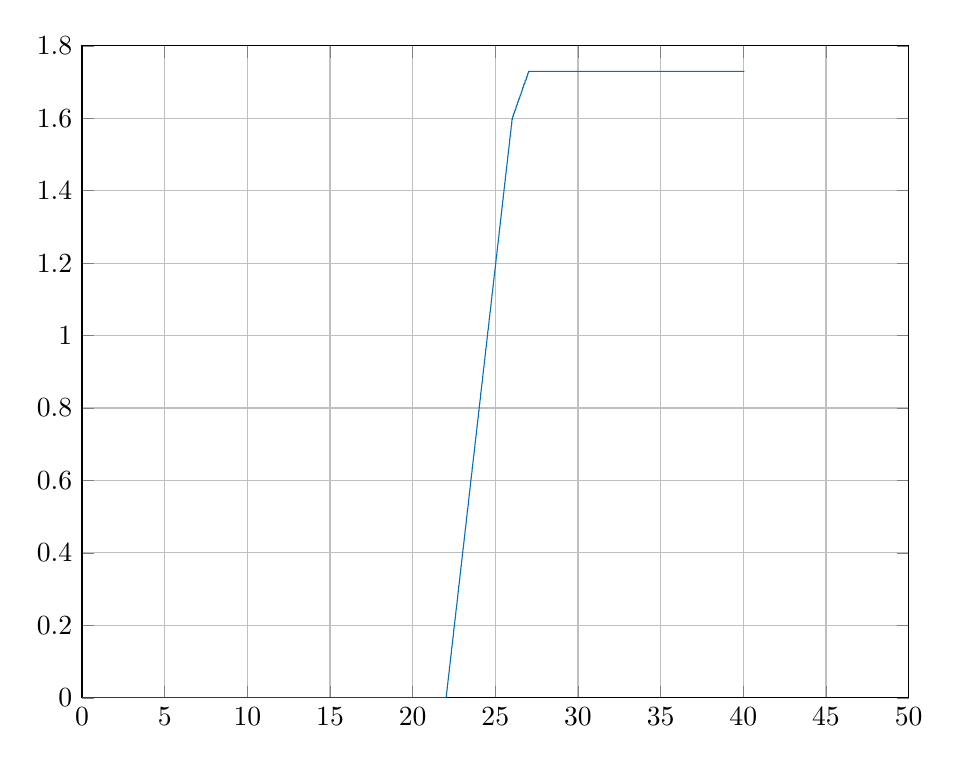
\begin{tikzpicture}

\begin{axis}[%
width=4.133in,
height=3.26in,
at={(0.693in,0.44in)},
scale only axis,
xmin=0,
xmax=50,
xmajorgrids,
ymin=0,
ymax=1.8,
ymajorgrids,
axis background/.style={fill=white}
]
\addplot [color=mycolor1,solid,forget plot]
  table[row sep=crcr]{%
0	0\\
0.0177441540000001	0\\
0.0327040630000001	0\\
0.0478449689999996	0\\
0.0659545939999996	0\\
0.080935841	0\\
0.095923176	0\\
0.11195197	0\\
0.128055795	0\\
0.143941748	0\\
0.159967933999999	0\\
0.176042313999999	0\\
0.191954450999999	0\\
0.208009254	0\\
0.22399488	0\\
0.239953013999999	0\\
0.256054853999999	0\\
0.272063669	0\\
0.288027004	0\\
0.303887813	0\\
0.319971607	0\\
0.335942635	0\\
0.352025743	0\\
0.3679568	0\\
0.383953943	0\\
0.399997912	0\\
0.415998250999999	0\\
0.431831394	0\\
0.447814032000001	0\\
0.463808589999999	0\\
0.479903010999999	0\\
0.495925008	0\\
0.511948347	0\\
0.528016396999999	0\\
0.543863147999999	0\\
0.562388751999999	0\\
0.577608655	0\\
0.592719001999999	0\\
0.608161168000001	0\\
0.624069551	0\\
0.639885296999999	0\\
0.655866359	0\\
0.671987365999999	0\\
0.68802496	0\\
0.703813795999999	0\\
0.719840768	0\\
0.738192618	0\\
0.753498854999999	0\\
0.768784837	0\\
0.784015643	0\\
0.79988878	0\\
0.815969871	0\\
0.831983674	0\\
0.848057242	0\\
0.863854896999999	0\\
0.879894759999999	0\\
0.896003269	0\\
0.911933238999999	0\\
0.928035511999999	0\\
0.943938683999999	0\\
0.960191785999999	0\\
0.975936873000001	0\\
0.991975221	0\\
1.007904933	0\\
1.025398666	0\\
1.040304124	0\\
1.055833496	0\\
1.07185873	0\\
1.090013931	0\\
1.10576894	0\\
1.120861382	0\\
1.13702896	0\\
1.152233154	0\\
1.167848246	0\\
1.183945535	0\\
1.199813575	0\\
1.21810959	0\\
1.233479532	0\\
1.248819967	0\\
1.264119629	0\\
1.2799481	0\\
1.29600457	0\\
1.311980842	0\\
1.327919031	0\\
1.343886916	0\\
1.362367992	0\\
1.377645444	0\\
1.392841231	0\\
1.408078793	0\\
1.424022405	0\\
1.44007512	0\\
1.456127821	0\\
1.472010755	0\\
1.488089533	0\\
1.505276587	0\\
1.52042763	0\\
1.53601755	0\\
1.551942352	0\\
1.567911675	0\\
1.583936325	0\\
1.59989258	0\\
1.615819365	0\\
1.632013797	0\\
1.647959463	0\\
1.663988703	0\\
1.679942628	0\\
1.695987233	0\\
1.712021079	0\\
1.727901406	0\\
1.743933763	0\\
1.762257126	0\\
1.777463037	0\\
1.792770717	0\\
1.808294613	0\\
1.823994137	0\\
1.839996003	0\\
1.856026653	0\\
1.87199263	0\\
1.887955314	0\\
1.903810895	0\\
1.919953914	0\\
1.937593507	0\\
1.952661926	0\\
1.968163942	0\\
1.984178283	0\\
1.999975183	0\\
2.017791296	0\\
2.033056711	0\\
2.047987846	0\\
2.063870266	0\\
2.079834083	0\\
2.096071024	0\\
2.111796419	0\\
2.128044492	0\\
2.143898936	0\\
2.162297373	0\\
2.177444796	0\\
2.192580046	0\\
2.208046917	0\\
2.223993811	0\\
2.239942403	0\\
2.255908685	0\\
2.271844786	0\\
2.290082946	0\\
2.305663551	0\\
2.321427334	0\\
2.337415825	0\\
2.353051482	0\\
2.368230299	0\\
2.384770288	0\\
2.400381588	0\\
2.416019773	0\\
2.432075243	0\\
2.447866992	0\\
2.464034625	0\\
2.479959588	0\\
2.49605535	0\\
2.511924627	0\\
2.528096842	0\\
2.543935965	0\\
2.562280086	0\\
2.577486766	0\\
2.592615542	0\\
2.607909968	0\\
2.624013005	0\\
2.639972317	0\\
2.656019128	0\\
2.671991098	0\\
2.68783833	0\\
2.70381914	0\\
2.719797684	0\\
2.735945271	0\\
2.751977241	0\\
2.767867978	0\\
2.7839776	0\\
2.799980396	0\\
2.816165123	0\\
2.832033263	0\\
2.847985654	0\\
2.864002992	0\\
2.879987682	0\\
2.895901791	0\\
2.912123187	0\\
2.928500747	0\\
2.943946666	0\\
2.959812605	0\\
2.976001123	0\\
2.991910687	0\\
3.0078866	0\\
3.024033743	0\\
3.039833721	0\\
3.055898507	0\\
3.071898381	0\\
3.088173756	0\\
3.104241709	0\\
3.119908618	0\\
3.135877983	0\\
3.151981441	0\\
3.167814753	0\\
3.184016414	0\\
3.200035055	0\\
3.215996707	0\\
3.232054362	0\\
3.247981445	0\\
3.264166714	0\\
3.279790125	0\\
3.296012658	0\\
3.311932396	0\\
3.328156619	0\\
3.343862637	0\\
3.360331353	0\\
3.376034386	0\\
3.391958477	0\\
3.407941351	0\\
3.423828912	0\\
3.442126699	0\\
3.457365924	0\\
3.472518824	0\\
3.487868274	0\\
3.503812755	0\\
3.519945999	0\\
3.536039249	0\\
3.551938139	0\\
3.568311326	0\\
3.58398362	0\\
3.599969341	0\\
3.615951755	0\\
3.63205545	0\\
3.64796565	0\\
3.665660884	0\\
3.680830758	0\\
3.696031371	0\\
3.711993129	0\\
3.728110995	0\\
3.743985369	0\\
3.760051875	0\\
3.775931153	0\\
3.792102727	0\\
3.808065336	0\\
3.823949485	0\\
3.839914836	0\\
3.856126292	0\\
3.873129683	0\\
3.888415745	0\\
3.904082118	0\\
3.919984447	0\\
3.936797435	0\\
3.95218989	0\\
3.968030944	0\\
3.983982969	0\\
4.000019606	0\\
4.01792116	0\\
4.032913303	0\\
4.047921539	0\\
4.063861382	0\\
4.079857392	0\\
4.095891563	0\\
4.111924659	0\\
4.128192669	0\\
4.143978449	0\\
4.160134024	0\\
4.175925001	0\\
4.191796591	0\\
4.208089832	0\\
4.223946351	0\\
4.239814982	0\\
4.255999085	0\\
4.271969471	0\\
4.290295194	0\\
4.305524384	0\\
4.320741453	0\\
4.335983263	0\\
4.351886062	0\\
4.368028138	0\\
4.383969334	0\\
4.399897934	0\\
4.415925558	0\\
4.431869626	0\\
4.447996477	0\\
4.46381962	0\\
4.479957766	0\\
4.495888877	0\\
4.511978467	0\\
4.527944261	0\\
4.544003875	0\\
4.560241184	0\\
4.575958202	0\\
4.592020126	0\\
4.607920568	0\\
4.624013937	0\\
4.640030653	0\\
4.655955594	0\\
4.671990289	0\\
4.688046214	0\\
4.703806353	0\\
4.719801313	0\\
4.736013502	0\\
4.751897951	0\\
4.768033836	0\\
4.784005832	0\\
4.799899736	0\\
4.815913036	0\\
4.83196671	0\\
4.847775381	0\\
4.863984264	0\\
4.879931643	0\\
4.896051845	0\\
4.911995762	0\\
4.92815309	0\\
4.94391307	0\\
4.960371144	0\\
4.975975883	0\\
4.991936031	0\\
5.00796669	0\\
5.025225409	0\\
5.040174419	0\\
5.055830857	0\\
5.071826165	0\\
5.087915419	0\\
5.103793775	0\\
5.119982737	0\\
5.13764764	0\\
5.152925242	0\\
5.168468381	0\\
5.183880225	0\\
5.199997693	0\\
5.215913877	0\\
5.231898023	0\\
5.247995057	0\\
5.2637976	0\\
5.279791141	0\\
5.296316409	0\\
5.311987624	0\\
5.328189245	0\\
5.343948408	0\\
5.359967983	0\\
5.375954299	0\\
5.391856128	0\\
5.408098391	0\\
5.424079379	0\\
5.440023342	0\\
5.456021868	0\\
5.471990165	0\\
5.488435392	0\\
5.503975324	0\\
5.519860487	0\\
5.535996266	0\\
5.552034071	0\\
5.567791657	0\\
5.583803568	0\\
5.600058789	0\\
5.615944598	0\\
5.632002603	0\\
5.647977485	0\\
5.664107499	0\\
5.679982405	0\\
5.695809307	0\\
5.711927927	0\\
5.727864808	0\\
5.743947707	0\\
5.760158351	0\\
5.775988783	0\\
5.792046087	0\\
5.808040178	0\\
5.823975249	0\\
5.839938834	0\\
5.856000936	0\\
5.871980058	0\\
5.888114707	0\\
5.903881931	0\\
5.922154549	0\\
5.935949996	0\\
5.952079521	0\\
5.967914484	0\\
5.983887847	0\\
6.00001967	0\\
6.018431561	0\\
6.033455699	0\\
6.048482665	0\\
6.063855193	0\\
6.07987279	0\\
6.095898001	0\\
6.111976692	0\\
6.128136278	0\\
6.143940917	0\\
6.159904689	0\\
6.175983181	0\\
6.191947174	0\\
6.207838687	0\\
6.224096146	0\\
6.239995549	0\\
6.256025953	0\\
6.271936895	0\\
6.2881028	0\\
6.303821208	0\\
6.319907718	0\\
6.33602018	0\\
6.351954771	0\\
6.367979261	0\\
6.383979535	0\\
6.3999932	0\\
6.415959658	0\\
6.431813065	0\\
6.44795526	0\\
6.46633681	0\\
6.481640492	0\\
6.496800582	0\\
6.512015123	0\\
6.528007565	0\\
6.544001335	0\\
6.560166974	0\\
6.575941672	0\\
6.591818356	0\\
6.607989749	0\\
6.623906393	0\\
6.64011637	0\\
6.655979844	0\\
6.673691636	0\\
6.688914219	0\\
6.704891777	0\\
6.720183131	0\\
6.737123565	0\\
6.752308488	0\\
6.768028357	0\\
6.783980568	0\\
6.799984341	0\\
6.815967206	0\\
6.83203869	0\\
6.847972771	0\\
6.864023079	0\\
6.879902425	0\\
6.895983262	0\\
6.912068584	0\\
6.928217671	0\\
6.943979611	0\\
6.960208831	0\\
6.975958476	0\\
6.992048525	0\\
7.007884522	0\\
7.025348728	0\\
7.040294171	0\\
7.055880966	0\\
7.071901506	0\\
7.08792888	0\\
7.103913066	0\\
7.120068382	0\\
7.137139436	0\\
7.152855242	0\\
7.168165895	0\\
7.183959671	0\\
7.19999932	0\\
7.215985663	0\\
7.231883992	0\\
7.247973186	0\\
7.263937812	0\\
7.280008721	0\\
7.295851106	0\\
7.312005332	0\\
7.328187843	0\\
7.343982595	0\\
7.36024405	0\\
7.375927101	0\\
7.391989892	0\\
7.4079011	0\\
7.42401634	0\\
7.440028795	0\\
7.456084628	0\\
7.471871999	0\\
7.487989159	0\\
7.504021292	0\\
7.519989669	0\\
7.536008014	0\\
7.551949195	0\\
7.567858875	0\\
7.583935748	0\\
7.601006903	0\\
7.616333011	0\\
7.631832045	0\\
7.648012658	0\\
7.66422105	0\\
7.679991222	0\\
7.695870973	0\\
7.711873373	0\\
7.728006439	0\\
7.743939256	0\\
7.76020953	0\\
7.775971928	0\\
7.792052602	0\\
7.807974727	0\\
7.823995777	0\\
7.840030888	0\\
7.855979139	0\\
7.872011384	0\\
7.8880804	0\\
7.903981492	0\\
7.920021161	0\\
7.93706545	0\\
7.952477327	0\\
7.9678801	0\\
7.983891723	0\\
8.000016786	0\\
8.017869878	0\\
8.032826874	0\\
8.047843233	0\\
8.065963524	0\\
8.080942145	0\\
8.096041817	0\\
8.112014951	0\\
8.12803528	0\\
8.14397842	0\\
8.16001178	0\\
8.176267969	0\\
8.191914898	0\\
8.207940751	0\\
8.224000021	0\\
8.240027206	0\\
8.256005689	0\\
8.272060388	0\\
8.288060868	0\\
8.30464051	0\\
8.320066414	0\\
8.335981801	0\\
8.352041405	0\\
8.367962458	0\\
8.383991149	0\\
8.399972366	0\\
8.416015853	0\\
8.432958448	0\\
8.448360829	0\\
8.463990804	0\\
8.480266458	0\\
8.495865174	0\\
8.511956939	0\\
8.527865723	0\\
8.544168528	0\\
8.559968157	0\\
8.578390398	0\\
8.593594679	0\\
8.608849229	0\\
8.624003037	0\\
8.640080341	0\\
8.655987797	0\\
8.671984308	0\\
8.687931107	0\\
8.704159782	0\\
8.719962013	0\\
8.735946497	0\\
8.752022388	0\\
8.767927688	0\\
8.783984821	0\\
8.800003878	0\\
8.816004223	0\\
8.831966095	0\\
8.848040975	0\\
8.863999835	0\\
8.880144963	0\\
8.895806699	0\\
8.912055063	0\\
8.927921969	0\\
8.944068836	0\\
8.959911623	0\\
8.978394041	0\\
8.993690196	0\\
9.008788051	0\\
9.023814294	0\\
9.041908105	0\\
9.05681926	0\\
9.071835365	0\\
9.087841756	0\\
9.103845233	0\\
9.119976837	0\\
9.136027025	0\\
9.151993408	0\\
9.167967223	0\\
9.183994778	0\\
9.199965717	0\\
9.215891879	0\\
9.231996951	0\\
9.247892359	0\\
9.263988631	0\\
9.280002711	0\\
9.295985623	0\\
9.311957464	0\\
9.327999411	0\\
9.344179888	0\\
9.360029036	0\\
9.376214415	0\\
9.392500602	0\\
9.408018805	0\\
9.423992344	0\\
9.439977644	0\\
9.455994021	0\\
9.472021477	0\\
9.488143487	0\\
9.50406149	0\\
9.519982771	0\\
9.53603548	0\\
9.552021988	0\\
9.567994715	0\\
9.584045985	0\\
9.599980426	0\\
9.616004284	0\\
9.631946195	0\\
9.648059476	0\\
9.663985559	0\\
9.679989567	0\\
9.69599361	0\\
9.711961915	0\\
9.727990195	0\\
9.744101561	0\\
9.759973811	0\\
9.778293465	0\\
9.793577786	0\\
9.808858878	0\\
9.824244693	0\\
9.840290734	0\\
9.856116657	0\\
9.872206048	0\\
9.887930688	0\\
9.903899309	0\\
9.919951271	0\\
9.935977203	0\\
9.951984689	0\\
9.967981481	0\\
9.983956633	0\\
9.999947442	0\\
10.017871321	0\\
10.032808961	0\\
10.047859833	0\\
10.063820433	0\\
10.0819286	0\\
10.09690558	0\\
10.112008278	0\\
10.127976725	0\\
10.144209833	0\\
10.159980776	0\\
10.176072019	0\\
10.192019298	0\\
10.207919569	0\\
10.223870053	0\\
10.239996002	0\\
10.25602208	0\\
10.272043914	0\\
10.28804911	0\\
10.304009835	0\\
10.319993903	0\\
10.336057205	0\\
10.352030243	0\\
10.367956325	0\\
10.384016425	0\\
10.399949676	0\\
10.415887273	0\\
10.431963201	0\\
10.448001658	0\\
10.46402966	0\\
10.480015026	0\\
10.495952148	0\\
10.511976326	0\\
10.5279805	0\\
10.544210234	0\\
10.559986281	0\\
10.575948973	0\\
10.591905897	0\\
10.608046685	0\\
10.623974856	0\\
10.639982006	0\\
10.656007648	0\\
10.672016717	0\\
10.688027015	0\\
10.703883115	0\\
10.719850408	0\\
10.736036028	0\\
10.751966715	0\\
10.768060426	0\\
10.784009615	0\\
10.799861772	0\\
10.815977265	0\\
10.832009553	0\\
10.847977785	0\\
10.864036139	0\\
10.88002107	0\\
10.896019403	0\\
10.911838149	0\\
10.927964589	0\\
10.944132473	0\\
10.960012842	0\\
10.97599494	0\\
10.991880004	0\\
11.007970899	0\\
11.025414481	0\\
11.040451894	0\\
11.055869466	0\\
11.071919421	0\\
11.087924862	0\\
11.103969424	0\\
11.1199788	0\\
11.135877788	0\\
11.151980131	0\\
11.167941124	0\\
11.183995078	0\\
11.200015884	0\\
11.215937089	0\\
11.232019305	0\\
11.248020617	0\\
11.26421936	0\\
11.280012	0\\
11.296021746	0\\
11.312080644	0\\
11.328057691	0\\
11.344028408	0\\
11.360011019	0\\
11.376003706	0\\
11.391936738	0\\
11.407981734	0\\
11.424002395	0\\
11.440014917	0\\
11.45609619	0\\
11.472070065	0\\
11.488103465	0\\
11.5039031	0\\
11.520077922	0\\
11.536003773	0\\
11.551989733	0\\
11.567961579	0\\
11.584026304	0\\
11.599964638	0\\
11.615866219	0\\
11.632051283	0\\
11.648008565	0\\
11.663991783	0\\
11.679955904	0\\
11.695908896	0\\
11.712044954	0\\
11.727984646	0\\
11.744266289	0\\
11.760126251	0\\
11.7760434	0\\
11.792132146	0\\
11.808050886	0\\
11.823997807	0\\
11.84004679	0\\
11.855996079	0\\
11.872030726	0\\
11.888012132	0\\
11.90389773	0\\
11.919992051	0\\
11.935992807	0\\
11.95189877	0\\
11.967868711	0\\
11.984037355	0\\
12.000105929	0\\
12.017849286	0\\
12.032768543	0\\
12.047866061	0\\
12.063880419	0\\
12.079877976	0\\
12.098046519	0\\
12.113407982	0\\
12.128578276	0\\
12.14398879	0\\
12.159980736	0\\
12.176133999	0\\
12.191915091	0\\
12.208001663	0\\
12.224002396	0\\
12.239964929	0\\
12.255964619	0\\
12.272018179	0\\
12.287907709	0\\
12.303960852	0\\
12.319980397	0\\
12.335941135	0\\
12.351983059	0\\
12.367987037	0\\
12.384113476	0\\
12.400041719	0\\
12.416061042	0\\
12.431941691	0\\
12.447990776	0\\
12.46400612	0\\
12.47986539	0\\
12.496005331	0\\
12.511977477	0\\
12.527990866	0\\
12.544075412	0\\
12.560051507	0\\
12.576208672	0\\
12.591987399	0\\
12.607988185	0\\
12.623998292	0\\
12.640042872	0\\
12.655954371	0\\
12.671993002	0\\
12.688069214	0\\
12.704052035	0\\
12.720157683	0\\
12.735883019	0\\
12.751988071	0\\
12.767953513	0\\
12.784022603	0\\
12.79994475	0\\
12.815851826	0\\
12.831979317	0\\
12.848006828	0\\
12.864024507	0\\
12.879993846	0\\
12.896013505	0\\
12.912028027	0\\
12.927939231	0\\
12.94406223	0\\
12.959992479	0\\
12.978385834	0\\
12.993673517	0\\
13.008884356	0\\
13.023873171	0\\
13.039965823	0\\
13.055962863	0\\
13.072056005	0\\
13.088051354	0\\
13.103908324	0\\
13.119826742	0\\
13.135977399	0\\
13.151916194	0\\
13.168070177	0\\
13.18398576	0\\
13.199890941	0\\
13.215990689	0\\
13.231990683	0\\
13.248005491	0\\
13.263988195	0\\
13.280023099	0\\
13.295914622	0\\
13.3120289	0\\
13.327973192	0\\
13.3463917	0\\
13.361635521	0\\
13.376936742	0\\
13.392542949	0\\
13.407984984	0\\
13.423990415	0\\
13.440035161	0\\
13.456027312	0\\
13.472029757	0\\
13.488019035	0\\
13.504048668	0\\
13.519997101	0\\
13.535957424	0\\
13.551978436	0\\
13.567960935	0\\
13.583982097	0\\
13.600088893	0\\
13.616051723	0\\
13.632095198	0\\
13.647936911	0\\
13.664018976	0\\
13.679929405	0\\
13.696115557	0\\
13.712088791	0\\
13.728079724	0\\
13.744146188	0\\
13.760004076	0\\
13.776138129	0\\
13.791990433	0\\
13.808319523	0\\
13.823991519	0\\
13.840876282	0\\
13.856198395	0\\
13.872022927	0\\
13.88799893	0\\
13.903902853	0\\
13.920299171	0\\
13.936524143	0\\
13.952003133	0\\
13.967922164	0\\
13.984021356	0\\
14.000004302	0\\
14.021512803	0\\
14.033500279	0\\
14.048825728	0\\
14.064094519	0\\
14.079982062	0\\
14.096036069	0\\
14.111978945	0\\
14.127970598	0\\
14.144272802	0\\
14.159927968	0\\
14.176001765	0\\
14.191993996	0\\
14.208044255	0\\
14.224030353	0\\
14.239899612	0\\
14.25595932	0\\
14.271973075	0\\
14.28807093	0\\
14.303881156	0\\
14.319956078	0\\
14.337491235	0\\
14.352804817	0\\
14.368146496	0\\
14.384045512	0\\
14.399862218	0\\
14.415813551	0\\
14.431962165	0\\
14.447932542	0\\
14.464199591	0\\
14.47987596	0\\
14.496005858	0\\
14.511931121	0\\
14.527984224	0\\
14.543959983	0\\
14.559920262	0\\
14.576162621	0\\
14.591981038	0\\
14.608046856	0\\
14.62399606	0\\
14.640035955	0\\
14.655874969	0\\
14.67200585	0\\
14.687913297	0\\
14.703887227	0\\
14.720035739	0\\
14.736084322	0\\
14.751996589	0\\
14.767982716	0\\
14.784021955	0\\
14.799951995	0\\
14.815974284	0\\
14.832722157	0\\
14.848035872	0\\
14.86398905	0\\
14.880026604	0\\
14.896024939	0\\
14.912215675	0\\
14.927989651	0\\
14.943997957	0\\
14.959906851	0\\
14.978305886	0\\
14.99354199	0\\
15.008697568	0\\
15.023974395	0\\
15.039986789	0\\
15.056140917	0\\
15.072027932	0\\
15.087898911	0\\
15.104072529	0\\
15.119999799	0\\
15.136014341	0\\
15.151948685	0\\
15.16794009	0\\
15.183979463	0\\
15.200022249	0\\
15.215902045	0\\
15.231979085	0\\
15.24810982	0\\
15.26400462	0\\
15.279983627	0\\
15.296015789	0\\
15.311988997	0\\
15.327958147	0\\
15.344116503	0\\
15.359944198	0\\
15.375985619	0\\
15.391964544	0\\
15.407926139	0\\
15.423929022	0\\
15.440027877	0\\
15.4559316	0\\
15.471922784	0\\
15.487959992	0\\
15.503849215	0\\
15.522218674	0\\
15.537355028	0\\
15.552485878	0\\
15.567856399	0\\
15.583983553	0\\
15.599907845	0\\
15.615964183	0\\
15.631958534	0\\
15.64799247	0\\
15.663977415	0\\
15.679929334	0\\
15.695828736	0\\
15.712003932	0\\
15.72812514	0\\
15.744129129	0\\
15.759839239	0\\
15.776051962	0\\
15.791962243	0\\
15.807942971	0\\
15.824014363	0\\
15.840027182	0\\
15.855982539	0\\
15.872008117	0\\
15.887972795	0\\
15.903826785	0\\
15.919920663	0\\
15.935967355	0\\
15.95200946	0\\
15.967943705	0\\
15.983972538	0\\
15.999983157	0\\
16.018615015	0\\
16.031993003	0\\
16.048060554	0\\
16.064007484	0\\
16.079901392	0\\
16.095854435	0\\
16.111999047	0\\
16.128037352	0\\
16.144240554	0\\
16.159954101	0\\
16.175951184	0\\
16.191984654	0\\
16.207904056	0\\
16.223985031	0\\
16.240024681	0\\
16.25600208	0\\
16.272006995	0\\
16.288044368	0\\
16.304065686	0\\
16.319995551	0\\
16.335958025	0\\
16.352009455	0\\
16.367880078	0\\
16.38399931	0\\
16.399958407	0\\
16.415849514	0\\
16.431883881	0\\
16.447992115	0\\
16.464002217	0\\
16.480128507	0\\
16.495935629	0\\
16.511965451	0\\
16.527942849	0\\
16.544002784	0\\
16.559951852	0\\
16.576310388	0\\
16.591993916	0\\
16.607981093	0\\
16.624099508	0\\
16.639977816	0\\
16.655957981	0\\
16.672075781	0\\
16.687981617	0\\
16.70408034	0\\
16.720016419	0\\
16.7359338	0\\
16.752928353	0\\
16.768076001	0\\
16.784042128	0\\
16.799941782	0\\
16.816403911	0\\
16.831945972	0\\
16.848033424	0\\
16.86404063	0\\
16.880056043	0\\
16.89597555	0\\
16.911809413	0\\
16.927964491	0\\
16.943859189	0\\
16.959847547	0\\
16.976306144	0\\
16.991895648	0\\
17.007861192	0\\
17.023903461	0\\
17.039888521	0\\
17.055981314	0\\
17.071804681	0\\
17.08812132	0\\
17.103986067	0\\
17.11994946	0\\
17.135943308	0\\
17.152028495	0\\
17.167997112	0\\
17.183813738	0\\
17.1999706	0\\
17.216001494	0\\
17.231945523	0\\
17.248143254	0\\
17.263959356	0\\
17.279957697	0\\
17.295903573	0\\
17.311831899	0\\
17.327913376	0\\
17.34387256	0\\
17.360021005	0\\
17.376265783	0\\
17.392021055	0\\
17.407958846	0\\
17.424052004	0\\
17.440041537	0\\
17.455980248	0\\
17.47205077	0\\
17.487902924	0\\
17.503972557	0\\
17.519909292	0\\
17.535974259	0\\
17.551906023	0\\
17.567973181	0\\
17.583989841	0\\
17.599989014	0\\
17.615818706	0\\
17.631799887	0\\
17.64796211	0\\
17.66402742	0\\
17.680030102	0\\
17.695854282	0\\
17.711905321	0\\
17.727900065	0\\
17.744114573	0\\
17.75999217	0\\
17.776111038	0\\
17.791797316	0\\
17.808062441	0\\
17.823913438	0\\
17.840021682	0\\
17.855995502	0\\
17.872057927	0\\
17.88793406	0\\
17.90402632	0\\
17.919969605	0\\
17.936015152	0\\
17.952047514	0\\
17.967998953	0\\
17.98408643	0\\
17.999937903	0\\
18.017713904	0\\
18.032926989	0\\
18.048076682	0\\
18.063924107	0\\
18.080003085	0\\
18.096008291	0\\
18.111842246	0\\
18.130062683	0\\
18.145491549	0\\
18.160759238	0\\
18.175956101	0\\
18.191884821	0\\
18.20806147	0\\
18.224692697	0\\
18.239952728	0\\
18.256008258	0\\
18.272024733	0\\
18.288010349	0\\
18.30410588	0\\
18.320001355	0\\
18.335972967	0\\
18.351979796	0\\
18.36816057	0\\
18.383868069	0\\
18.400025477	0\\
18.416136989	0\\
18.431947889	0\\
18.447949276	0\\
18.463946043	0\\
18.479997801	0\\
18.496050152	0\\
18.511806667	0\\
18.527798792	0\\
18.543893029	0\\
18.559880903	0\\
18.576054051	0\\
18.591822555	0\\
18.607864675	0\\
18.623982842	0\\
18.640034433	0\\
18.655940578	0\\
18.671970701	0\\
18.688088237	0\\
18.704055742	0\\
18.719847187	0\\
18.735947129	0\\
18.751992392	0\\
18.767902927	0\\
18.783831042	0\\
18.7999934	0\\
18.815810661	0\\
18.834114914	0\\
18.84946709	0\\
18.864867929	0\\
18.880255113	0\\
18.895962589	0\\
18.911859012	0\\
18.927977997	0\\
18.943940977	0\\
18.959923903	0\\
18.976041518	0\\
18.991981506	0\\
19.007935539	0\\
19.025572889	0\\
19.040871928	0\\
19.056438628	0\\
19.072266862	0\\
19.087987123	0\\
19.104017448	0\\
19.120041113	0\\
19.136089582	0\\
19.152001241	0\\
19.167970653	0\\
19.183993411	0\\
19.19997326	0\\
19.217370569	0\\
19.232709265	0\\
19.248086704	0\\
19.263974539	0\\
19.280053441	0\\
19.295960011	0\\
19.311846466	0\\
19.330104587	0\\
19.345462389	0\\
19.36091123	0\\
19.376104842	0\\
19.391941061	0\\
19.407895005	0\\
19.424153682	0\\
19.439978196	0\\
19.455975314	0\\
19.472029896	0\\
19.487922857	0\\
19.50403235	0\\
19.519984596	0\\
19.536018948	0\\
19.552021052	0\\
19.567933364	0\\
19.584057507	0\\
19.599982401	0\\
19.616378024	0\\
19.631959547	0\\
19.647867944	0\\
19.663884525	0\\
19.680028676	0\\
19.69598001	0\\
19.711797359	0\\
19.729901931	0\\
19.745080392	0\\
19.760194592	0\\
19.77598209	0\\
19.791910871	0\\
19.808114813	0\\
19.823910719	0\\
19.839977941	0\\
19.856102042	0\\
19.872069051	0\\
19.887886331	0\\
19.904063416	0\\
19.919879187	0\\
19.935990063	0\\
19.952153276	0\\
19.967911568	0\\
19.984041665	0\\
19.999969177	0\\
20.017754685	0\\
20.033065576	0\\
20.048261028	0\\
20.065148395	0\\
20.080584776	0\\
20.095921297	0\\
20.112314658	0\\
20.128072212	0\\
20.144050322	0\\
20.160008674	0\\
20.176244886	0\\
20.191946088	0\\
20.208192053	0\\
20.223937571	0\\
20.240101997	0\\
20.255949027	0\\
20.272073862	0\\
20.288048639	0\\
20.303961711	0\\
20.320062529	0\\
20.336051327	0\\
20.351867158	0\\
20.367998558	0\\
20.384235131	0\\
20.399970861	0\\
20.416047321	0\\
20.432002035	0\\
20.447985038	0\\
20.463823328	0\\
20.479886681	0\\
20.495986982	0\\
20.511926494	0\\
20.527922729	0\\
20.543957572	0\\
20.559990106	0\\
20.575967763	0\\
20.592058742	0\\
20.60784029	0\\
20.623964623	0\\
20.639915171	0\\
20.655942033	0\\
20.672022121	0\\
20.687986574	0\\
20.707530295	0\\
20.7198142	0\\
20.735799943	0\\
20.754076883	0\\
20.769131774	0\\
20.785242884	0\\
20.800413404	0\\
20.815900959	0\\
20.831911751	0\\
20.847991349	0\\
20.864215246	0\\
20.880172489	0\\
20.89604119	0\\
20.912091578	0\\
20.927945847	0\\
20.944081173	0\\
20.960066684	0\\
20.975969002	0\\
20.991931671	0\\
21.007976778	0\\
21.025607157	0\\
21.041084259	0\\
21.056381035	0\\
21.071975516	0\\
21.08800851	0\\
21.104036106	0\\
21.11978888	0\\
21.136058816	0\\
21.151994684	0\\
21.167953509	0\\
21.184001052	0\\
21.199977548	0\\
21.215797052	0\\
21.234055508	0\\
21.249365023	0\\
21.264517231	0\\
21.280016451	0\\
21.295960836	0\\
21.311862378	0\\
21.327983413	0\\
21.34406115	0\\
21.359918185	0\\
21.375870588	0\\
21.391958276	0\\
21.408024456	0\\
21.423858845	0\\
21.439904702	0\\
21.455890771	0\\
21.472065636	0\\
21.487990324	0\\
21.503924697	0\\
21.519952902	0\\
21.536053434	0\\
21.552156546	0\\
21.567988841	0\\
21.583994477	0\\
21.59996743	0\\
21.615992246	0\\
21.655064028	0\\
21.670173849	0\\
21.686191848	0\\
21.702176256	0\\
21.718242571	0\\
21.734196731	0\\
21.752411665	0\\
21.767800269	0\\
21.783079991	0\\
21.798362695	0\\
21.814357483	0\\
21.830303609	0\\
21.846278672	0\\
21.862192804	0\\
21.880667552	0\\
21.895776652	0\\
21.910926669	0\\
21.926283994	0\\
21.944665708	0\\
21.959741178	0\\
21.974922207	0\\
21.990247147	0\\
22.006397717	0\\
22.023988324	0.00196265250093623\\
22.039055139	0.00588782309712144\\
22.05430491	0.0137378271094637\\
22.070331314	0.0180483095532901\\
22.086381205	0.0243211223106177\\
22.102324425	0.0349037381639916\\
22.11844384	0.0372525409112749\\
22.134320397	0.0451024846421164\\
22.150300566	0.0509900495807489\\
22.166279265	0.0568771427074427\\
22.182322897	0.0647266827313098\\
22.198249003	0.0690376659754403\\
22.214245136	0.0753108401078128\\
22.230301005	0.0862812586487168\\
22.246394786	0.0882437976568816\\
22.262230523	0.0960930788631625\\
22.278448973	0.101980106548511\\
22.294239367	0.107866668964832\\
22.310426027	0.115715468385378\\
22.326201298	0.12002687706296\\
22.342466703	0.126300396507757\\
22.358312833	0.136884975424979\\
22.374320144	0.139235086555282\\
22.390375329	0.1470836920051\\
22.406225986	0.15297027106607\\
22.422235792	0.15885635045153\\
22.438465649	0.166704549779748\\
22.454329415	0.171016583078527\\
22.470383371	0.17729046311912\\
22.486352676	0.187875869136671\\
22.502240175	0.192188863893721\\
22.518396709	0.198074482817265\\
22.534244035	0.20396050407154\\
22.550249363	0.209846057649824\\
22.566291798	0.217693447243858\\
22.582415262	0.222005959012147\\
22.5984103	0.228280326950425\\
22.614325262	0.238479535972078\\
22.630270806	0.243180244429294\\
22.64632788	0.249065228270173\\
22.662287485	0.254950792897375\\
22.680877012	0.260835853280376\\
22.696397841	0.268682699723232\\
22.711552355	0.274567647842122\\
22.726574298	0.281232042751927\\
22.742327242	0.28907848018076\\
22.758279839	0.294171497626362\\
22.774478613	0.300056089859967\\
22.790305551	0.309864098850856\\
22.806395373	0.311825621819897\\
22.822354675	0.319671643134187\\
22.838466497	0.325556305588455\\
22.854355785	0.332221740704128\\
22.870407877	0.340067554629623\\
22.88631445	0.345162899144574\\
22.902387617	0.351046943950282\\
22.918459556	0.360853983964899\\
22.934269089	0.36281543667645\\
22.950361492	0.370660705553917\\
22.96629014	0.376936013254002\\
22.982346792	0.383211592093098\\
22.998236221	0.391449238896718\\
23.019628587	0.398115348909671\\
23.031469793	0.403998964688387\\
23.046564953	0.411843965087871\\
23.062298764	0.413805058741265\\
23.078402653	0.421649763121828\\
23.094178311	0.427925287928286\\
23.110200395	0.434201207878475\\
23.127454235	0.44243923506565\\
23.143406326	0.447145421266491\\
23.158732463	0.453028415736072\\
23.174360877	0.462833719844635\\
23.190324647	0.466756188006447\\
23.206298972	0.472638696574248\\
23.222169591	0.478914523300112\\
23.238559523	0.485190794301947\\
23.254371491	0.493428744342509\\
23.270249796	0.500097345551876\\
23.286372482	0.504019054265204\\
23.302282086	0.513823554756014\\
23.318186828	0.517745488092429\\
23.334156421	0.523627574221056\\
23.350343948	0.529903769743589\\
23.366284072	0.536180453424628\\
23.382328887	0.544418667427697\\
23.398255897	0.54912757780595\\
23.414166942	0.556970254100018\\
23.430330648	0.564813053342594\\
23.446383868	0.568734821114503\\
23.462191018	0.574616259106889\\
23.478430311	0.582853268079862\\
23.494241708	0.58716965955018\\
23.510470816	0.595803560963653\\
23.526358042	0.602078852989293\\
23.542700745	0.607960466546468\\
23.558199073	0.615802495024335\\
23.574375386	0.619723769078695\\
23.590330593	0.625604757919442\\
23.606500598	0.635802425644029\\
23.622688537	0.638158989803058\\
23.638185474	0.646793625294386\\
23.654196095	0.653069332399784\\
23.670408415	0.658950332584922\\
23.686326759	0.666791751472149\\
23.702264482	0.670712809654558\\
23.718290795	0.676592967091962\\
23.734374509	0.686790642733639\\
23.750286653	0.689147835126509\\
23.766291469	0.698178695539595\\
23.78234744	0.704059634548842\\
23.798177011	0.709940187011015\\
23.814320352	0.717780776992039\\
23.830228216	0.721701303004489\\
23.846288473	0.727581227441712\\
23.862190859	0.737778817999552\\
23.878302401	0.740136497297147\\
23.894256324	0.749169330642184\\
23.910209326	0.755049696763626\\
23.928327762	0.760929580551688\\
23.943538498	0.768769527628751\\
23.958722043	0.772689834404467\\
23.974378754	0.778568941406616\\
23.990177182	0.789165099570481\\
24.00855221	0.793085353935178\\
24.022871924	0.800159599431706\\
24.038509697	0.807999237029899\\
24.054292439	0.811918937918927\\
24.070268278	0.819758071006196\\
24.086144764	0.823677833565138\\
24.102335473	0.829556682908028\\
24.118289543	0.840153596068286\\
24.134209088	0.844473718510547\\
24.150364932	0.851149686339819\\
24.16630243	0.857028937192202\\
24.18243555	0.862907679862328\\
24.198321486	0.870746222510152\\
24.214354372	0.874665543888288\\
24.230180066	0.880543577384739\\
24.246290664	0.891141544959315\\
24.262274475	0.895862696960028\\
24.278342243	0.90213931593016\\
24.294426776	0.909977518864959\\
24.310343148	0.913896486284602\\
24.326225234	0.92173393147615\\
24.342217303	0.927612348435594\\
24.360546942	0.933890838043761\\
24.375647749	0.942129380591523\\
24.390990519	0.946851919225665\\
24.406294182	0.953128747489676\\
24.422268531	0.962925377587285\\
24.438308004	0.964884472093195\\
24.454332951	0.972721576855379\\
24.470233269	0.978599193509023\\
24.486268323	0.984877768455997\\
24.502342485	0.993116603215289\\
24.518159415	0.997840386602373\\
24.534170077	1.0041175632084\\
24.550332823	1.01391337846501\\
24.56636199	1.01587223259384\\
24.582348102	1.02370850342089\\
24.598328392	1.02958559974022\\
24.61425054	1.03626776577397\\
24.630282536	1.04450715596784\\
24.646314333	1.04922962941131\\
24.66241766	1.05510628110657\\
24.678344394	1.06490084757692\\
24.69437882	1.06685970298689\\
24.710248503	1.07469535768219\\
24.726220501	1.08057182192994\\
24.742386991	1.08725481491809\\
24.758171706	1.09549459045194\\
24.774276598	1.10021825400664\\
24.790359155	1.10609416527933\\
24.806220989	1.11588817418989\\
24.822354658	1.11784657191708\\
24.838330041	1.12568112591984\\
24.854223247	1.13196118509653\\
24.870422163	1.13824142277462\\
24.886866671	1.14688620550705\\
24.902317714	1.15316488005878\\
24.918228638	1.15708174450331\\
24.934330968	1.16687469330637\\
24.950296628	1.16883298478745\\
24.966439927	1.17666733201016\\
24.982181905	1.18294717200749\\
24.998338685	1.18922786462291\\
25.019140482	1.19787345918613\\
25.031151038	1.2021939950681\\
25.04632837	1.21002739740136\\
25.062254328	1.21786106991685\\
25.07828592	1.21981899732522\\
25.094461408	1.22765201807498\\
25.110176998	1.23629723343006\\
25.126163718	1.24062037915038\\
25.142242643	1.24886010114132\\
25.158240413	1.25318127687609\\
25.174292944	1.2590554019773\\
25.19017162	1.26884624490905\\
25.206191876	1.27080433595704\\
25.222269787	1.27863653569562\\
25.238238855	1.28728251649439\\
25.256529852	1.2920137289348\\
25.272086529	1.30025146250009\\
25.28706972	1.30416772230268\\
25.302328479	1.31199963946133\\
25.318327917	1.31983183266723\\
25.334252533	1.32374735391161\\
25.350385947	1.33002802844821\\
25.366357627	1.33826789687623\\
25.382352689	1.34300004128353\\
25.398467113	1.35123770067406\\
25.414221319	1.35515389731171\\
25.430408024	1.36298476920618\\
25.446212433	1.37081574918354\\
25.464439046	1.37473165363319\\
25.479621267	1.38142102021264\\
25.49472912	1.3916193074079\\
25.510384383	1.39398574941582\\
25.526536748	1.40222342759882\\
25.542392689	1.4080963948855\\
25.558391582	1.41396929142831\\
25.574182136	1.42179943970832\\
25.590396774	1.42571482611862\\
25.606315667	1.4324053539943\\
25.622186452	1.44301377537657\\
25.638168271	1.4453784049338\\
25.654182391	1.45320864718292\\
25.670203463	1.45908143988643\\
25.686304702	1.46495295770858\\
25.702142729	1.47278276169963\\
25.720392975	1.47751791749954\\
25.735504011	1.48338923249167\\
25.750497624	1.49399820212478\\
25.766330907	1.49636387362498\\
25.782142986	1.50419302864838\\
25.800180284	1.51202207510228\\
25.815242579	1.51593651993322\\
25.830473416	1.52376508317069\\
25.846232104	1.52850129776014\\
25.862354178	1.53478446038422\\
25.878265906	1.54498187507751\\
25.894347376	1.54734818560242\\
25.91036042	1.55517664296686\\
25.926333271	1.56104822011759\\
25.942327844	1.56691876082406\\
25.958210236	1.57515843310784\\
25.976436178	1.57948482942868\\
25.991580363	1.58617998191716\\
26.006959245	1.59637534990291\\
26.024235248	1.59637511431624\\
26.039267488	1.60224534794807\\
26.054277042	1.60420204283627\\
26.070167825	1.60615867185836\\
26.086260823	1.6061578488929\\
26.102151778	1.612027967353\\
26.118181712	1.61202756894149\\
26.13432692	1.61398360022728\\
26.150200076	1.61593944803289\\
26.1663409	1.61593903980029\\
26.182296298	1.6218086539615\\
26.198312342	1.62180753586554\\
26.214310844	1.62376391987536\\
26.230265631	1.62571947899068\\
26.2462289	1.62696085426466\\
26.262379877	1.63324449311547\\
26.278300511	1.63324449311547\\
26.294359329	1.63520034337774\\
26.310370588	1.63715660875594\\
26.326516458	1.63756843553285\\
26.342636789	1.64343735260555\\
26.358333657	1.64343695052131\\
26.374295671	1.64539328586717\\
26.39031626	1.6473489620994\\
26.406390167	1.64930503146661\\
26.422336635	1.65321736283439\\
26.438388681	1.65321643383888\\
26.454356703	1.65517197721347\\
26.470336431	1.65712793082226\\
26.486230453	1.65908371102238\\
26.502330661	1.66299509418414\\
26.518147054	1.66299459778688\\
26.53417113	1.66494985115996\\
26.550368614	1.6669055064385\\
26.566345426	1.67081714686794\\
26.582350471	1.67277271935071\\
26.598330385	1.67277143950487\\
26.623998244	1.67793273278838\\
26.630175521	1.67834865005335\\
26.646173326	1.6822601578852\\
26.662223168	1.68421582294451\\
26.678223535	1.68421515141987\\
26.694342251	1.68658531711789\\
26.71034016	1.68854049724439\\
26.726521206	1.69440846027549\\
26.74244475	1.69440751093652\\
26.758373091	1.69440652030594\\
26.774301207	1.69636217445991\\
26.79029648	1.69831706327394\\
26.806365657	1.70418391821695\\
26.822282652	1.70418341229416\\
26.838361476	1.70418227585839\\
26.854343001	1.70613702947508\\
26.870395761	1.70809229888722\\
26.886328543	1.71395864369089\\
26.902260285	1.71395798168635\\
26.918198218	1.71395729879783\\
26.934154711	1.71786827082108\\
26.950352974	1.71786612832197\\
26.966294747	1.7237327178115\\
26.982275437	1.72498872266842\\
26.998444123	1.72540639536885\\
27.019333815	1.72931723879723\\
27.031206463	1.72931654577744\\
27.046472644	1.72931612055085\\
27.062339693	1.72931612055085\\
27.078343179	1.72931612055085\\
27.094539878	1.72931612055085\\
27.110444733	1.72931612055085\\
27.126414222	1.72931612055085\\
27.142344233	1.72931612055085\\
27.158330115	1.72931612055085\\
27.174293356	1.72931612055085\\
27.190432098	1.72931612055085\\
27.206248855	1.72931612055085\\
27.222432874	1.72931612055085\\
27.238301631	1.72931612055085\\
27.254303991	1.72931612055085\\
27.270635766	1.72931612055085\\
27.286277598	1.72931612055085\\
27.302338254	1.72931612055085\\
27.318165342	1.72931612055085\\
27.334359687	1.72931612055085\\
27.35033754	1.72931612055085\\
27.366170499	1.72931612055085\\
27.382330342	1.72931612055085\\
27.398309848	1.72931612055085\\
27.414380358	1.72931612055085\\
27.430488232	1.72931612055085\\
27.44643189	1.72931612055085\\
27.462370393	1.72931612055085\\
27.478288669	1.72931612055085\\
27.496720725	1.72931612055085\\
27.511956949	1.72931612055085\\
27.527137468	1.72931612055085\\
27.54240456	1.72931612055085\\
27.558355809	1.72931612055085\\
27.574328803	1.72931612055085\\
27.590349212	1.72931612055085\\
27.606358677	1.72931612055085\\
27.622280033	1.72931612055085\\
27.638364331	1.72931612055085\\
27.654446103	1.72931612055085\\
27.670268076	1.72931612055085\\
27.686173776	1.72931612055085\\
27.719030526	1.72931612055085\\
27.735075717	1.72931612055085\\
27.751093501	1.72931612055085\\
27.767049159	1.72931612055085\\
27.783097455	1.72931612055085\\
27.799098514	1.72931612055085\\
27.815250921	1.72931612055085\\
27.831271767	1.72931612055085\\
27.847312228	1.72931612055085\\
27.863131055	1.72931612055085\\
27.879213798	1.72931612055085\\
27.895208294	1.72931612055085\\
27.911220526	1.72931612055085\\
27.927194339	1.72931612055085\\
27.9431723	1.72931612055085\\
27.959520713	1.72931612055085\\
27.975158815	1.72931612055085\\
27.991204791	1.72931612055085\\
28.007168107	1.72931612055085\\
28.024759165	1.72931612055085\\
28.03916397	1.72931612055085\\
28.055328858	1.72931612055085\\
28.071123681	1.72931612055085\\
28.087179867	1.72931612055085\\
28.103215152	1.72931612055085\\
28.119020403	1.72931612055085\\
28.137149918	1.72931612055085\\
28.152357627	1.72931612055085\\
28.167548669	1.72931612055085\\
28.183226684	1.72931612055085\\
28.199257532	1.72931612055085\\
28.215214795	1.72931612055085\\
28.231215865	1.72931612055085\\
28.247136926	1.72931612055085\\
28.263180299	1.72931612055085\\
28.279120863	1.72931612055085\\
28.295228677	1.72931612055085\\
28.311224629	1.72931612055085\\
28.327183392	1.72931612055085\\
28.343277864	1.72931612055085\\
28.359190185	1.72931612055085\\
28.3752436	1.72931612055085\\
28.391272344	1.72931612055085\\
28.40713285	1.72931612055085\\
28.423215148	1.72931612055085\\
28.439229806	1.72931612055085\\
28.455096114	1.72931612055085\\
28.471240582	1.72931612055085\\
28.487312208	1.72931612055085\\
28.503094577	1.72931612055085\\
28.519025287	1.72931612055085\\
28.53504709	1.72931612055085\\
28.55119733	1.72931612055085\\
28.567215089	1.72931612055085\\
28.583237694	1.72931612055085\\
28.599130151	1.72931612055085\\
28.615188817	1.72931612055085\\
28.631219034	1.72931612055085\\
28.647134746	1.72931612055085\\
28.663187656	1.72931612055085\\
28.679140584	1.72931612055085\\
28.695153261	1.72931612055085\\
28.711199465	1.72931612055085\\
28.727282942	1.72931612055085\\
28.743135156	1.72931612055085\\
28.759504863	1.72931612055085\\
28.775167797	1.72931612055085\\
28.791215195	1.72931612055085\\
28.807197627	1.72931612055085\\
28.823235199	1.72931612055085\\
28.839171798	1.72931612055085\\
28.855274927	1.72931612055085\\
28.871322067	1.72931612055085\\
28.887087775	1.72931612055085\\
28.903315521	1.72931612055085\\
28.919172491	1.72931612055085\\
28.935137292	1.72931612055085\\
28.95115737	1.72931612055085\\
28.967286687	1.72931612055085\\
28.983093588	1.72931612055085\\
28.99921377	1.72931612055085\\
29.020118709	1.72931612055085\\
29.032143043	1.72931612055085\\
29.04743031	1.72931612055085\\
29.063237173	1.72931612055085\\
29.079186787	1.72931612055085\\
29.09521026	1.72931612055085\\
29.111259421	1.72931612055085\\
29.127156918	1.72931612055085\\
29.143218523	1.72931612055085\\
29.15930211	1.72931612055085\\
29.175217517	1.72931612055085\\
29.19122775	1.72931612055085\\
29.207224717	1.72931612055085\\
29.223212618	1.72931612055085\\
29.239281804	1.72931612055085\\
29.255377284	1.72931612055085\\
29.271270126	1.72931612055085\\
29.287193641	1.72931612055085\\
29.303207456	1.72931612055085\\
29.319215696	1.72931612055085\\
29.33522306	1.72931612055085\\
29.351245555	1.72931612055085\\
29.367110493	1.72931612055085\\
29.383232739	1.72931612055085\\
29.399274843	1.72931612055085\\
29.415114943	1.72931612055085\\
29.431206031	1.72931612055085\\
29.447206987	1.72931612055085\\
29.463189241	1.72931612055085\\
29.479206619	1.72931612055085\\
29.495190478	1.72931612055085\\
29.51119154	1.72931612055085\\
29.52958329	1.72931612055085\\
29.544659521	1.72931612055085\\
29.559801903	1.72931612055085\\
29.575254682	1.72931612055085\\
29.591209629	1.72931612055085\\
29.607026912	1.72931612055085\\
29.625414226	1.72931612055085\\
29.640730807	1.72931612055085\\
29.655994353	1.72931612055085\\
29.671139312	1.72931612055085\\
29.687224587	1.72931612055085\\
29.703031675	1.72931612055085\\
29.719074687	1.72931612055085\\
29.735237349	1.72931612055085\\
29.75123185	1.72931612055085\\
29.76724116	1.72931612055085\\
29.783195079	1.72931612055085\\
29.799303985	1.72931612055085\\
29.815245557	1.72931612055085\\
29.831318362	1.72931612055085\\
29.847186559	1.72931612055085\\
29.86317547	1.72931612055085\\
29.879152447	1.72931612055085\\
29.895281118	1.72931612055085\\
29.911228848	1.72931612055085\\
29.927216077	1.72931612055085\\
29.943234113	1.72931612055085\\
29.959540115	1.72931612055085\\
29.977023485	1.72931612055085\\
29.992197578	1.72931612055085\\
30.007443899	1.72931612055085\\
30.02484184	1.72931612055085\\
30.04003791	1.72931612055085\\
30.055263753	1.72931612055085\\
30.071304876	1.72931612055085\\
30.087284849	1.72931612055085\\
30.103217907	1.72931612055085\\
30.119249873	1.72931612055085\\
30.135153627	1.72931612055085\\
30.151063444	1.72931612055085\\
30.167217592	1.72931612055085\\
30.183298259	1.72931612055085\\
30.199232869	1.72931612055085\\
30.215176395	1.72931612055085\\
30.231212958	1.72931612055085\\
30.247380221	1.72931612055085\\
30.263170617	1.72931612055085\\
30.279236067	1.72931612055085\\
30.29524439	1.72931612055085\\
30.311189433	1.72931612055085\\
30.329670975	1.72931612055085\\
30.344985235	1.72931612055085\\
30.360344327	1.72931612055085\\
30.375516236	1.72931612055085\\
30.391363579	1.72931612055085\\
30.407215568	1.72931612055085\\
30.423240823	1.72931612055085\\
30.439305985	1.72931612055085\\
30.455232388	1.72931612055085\\
30.471254166	1.72931612055085\\
30.487148531	1.72931612055085\\
30.505375119	1.72931612055085\\
30.520681111	1.72931612055085\\
30.536056068	1.72931612055085\\
30.551319635	1.72931612055085\\
30.567217745	1.72931612055085\\
30.583058304	1.72931612055085\\
30.599221912	1.72931612055085\\
30.615259079	1.72931612055085\\
30.631271805	1.72931612055085\\
30.647229989	1.72931612055085\\
30.663458166	1.72931612055085\\
30.679151412	1.72931612055085\\
30.695233676	1.72931612055085\\
30.711058887	1.72931612055085\\
30.727045985	1.72931612055085\\
30.75490632	1.72931612055085\\
30.763624625	1.72931612055085\\
30.775545112	1.72931612055085\\
30.791088079	1.72931612055085\\
30.807297415	1.72931612055085\\
30.825937383	1.72931612055085\\
30.839252786	1.72931612055085\\
30.855233205	1.72931612055085\\
30.871216978	1.72931612055085\\
30.887219999	1.72931612055085\\
30.903235975	1.72931612055085\\
30.919210786	1.72931612055085\\
30.935233757	1.72931612055085\\
30.951213231	1.72931612055085\\
30.967235358	1.72931612055085\\
30.983188431	1.72931612055085\\
30.999216774	1.72931612055085\\
31.017936925	1.72931612055085\\
31.033276264	1.72931612055085\\
31.04868307	1.72931612055085\\
31.064165665	1.72931612055085\\
31.079514664	1.72931612055085\\
31.095351714	1.72931612055085\\
31.111034839	1.72931612055085\\
31.127148068	1.72931612055085\\
31.143199096	1.72931612055085\\
31.159345436	1.72931612055085\\
31.175212348	1.72931612055085\\
31.191184266	1.72931612055085\\
31.207252758	1.72931612055085\\
31.223225039	1.72931612055085\\
31.239134144	1.72931612055085\\
31.255560974	1.72931612055085\\
31.27107972	1.72931612055085\\
31.287171758	1.72931612055085\\
31.303247139	1.72931612055085\\
31.319209483	1.72931612055085\\
31.335190363	1.72931612055085\\
31.351095654	1.72931612055085\\
31.367107767	1.72931612055085\\
31.38320764	1.72931612055085\\
31.399308458	1.72931612055085\\
31.415100041	1.72931612055085\\
31.431041635	1.72931612055085\\
31.447188292	1.72931612055085\\
31.463090824	1.72931612055085\\
31.479182738	1.72931612055085\\
31.495294445	1.72931612055085\\
31.51151139	1.72931612055085\\
31.527134786	1.72931612055085\\
31.54319205	1.72931612055085\\
31.559301783	1.72931612055085\\
31.57521718	1.72931612055085\\
31.591226806	1.72931612055085\\
31.607193407	1.72931612055085\\
31.623235537	1.72931612055085\\
31.639127693	1.72931612055085\\
31.655226272	1.72931612055085\\
31.671139659	1.72931612055085\\
31.687317576	1.72931612055085\\
31.703727255	1.72931612055085\\
31.71931342	1.72931612055085\\
31.735231352	1.72931612055085\\
31.751460681	1.72931612055085\\
31.767177218	1.72931612055085\\
31.783250798	1.72931612055085\\
31.799188046	1.72931612055085\\
31.815097946	1.72931612055085\\
31.831226044	1.72931612055085\\
31.847192508	1.72931612055085\\
31.863226095	1.72931612055085\\
31.879218741	1.72931612055085\\
31.89519377	1.72931612055085\\
31.911405468	1.72931612055085\\
31.927253908	1.72931612055085\\
31.94306244	1.72931612055085\\
31.961186856	1.72931612055085\\
31.976265233	1.72931612055085\\
31.991262475	1.72931612055085\\
32.007106942	1.72931612055085\\
32.023086773	1.72931612055085\\
32.040123036	1.72931612055085\\
32.055169901	1.72931612055085\\
32.072137629	1.72931612055085\\
32.0874407	1.72931612055085\\
32.103262105	1.72931612055085\\
32.119194896	1.72931612055085\\
32.135386945	1.72931612055085\\
32.151092181	1.72931612055085\\
32.167208169	1.72931612055085\\
32.183211738	1.72931612055085\\
32.199146512	1.72931612055085\\
32.215208201	1.72931612055085\\
32.231292085	1.72931612055085\\
32.247191556	1.72931612055085\\
32.263443431	1.72931612055085\\
32.279232602	1.72931612055085\\
32.295248191	1.72931612055085\\
32.311183728	1.72931612055085\\
32.327478378	1.72931612055085\\
32.343077303	1.72931612055085\\
32.361332649	1.72931612055085\\
32.376582879	1.72931612055085\\
32.391757437	1.72931612055085\\
32.407194879	1.72931612055085\\
32.423214848	1.72931612055085\\
32.439124963	1.72931612055085\\
32.455197697	1.72931612055085\\
32.471265824	1.72931612055085\\
32.487209442	1.72931612055085\\
32.503224575	1.72931612055085\\
32.519233875	1.72931612055085\\
32.535158323	1.72931612055085\\
32.551172274	1.72931612055085\\
32.567180032	1.72931612055085\\
32.583173024	1.72931612055085\\
32.599204038	1.72931612055085\\
32.615132213	1.72931612055085\\
32.631098545	1.72931612055085\\
32.647192409	1.72931612055085\\
32.663191144	1.72931612055085\\
32.679227085	1.72931612055085\\
32.6952052	1.72931612055085\\
32.711143344	1.72931612055085\\
32.729500091	1.72931612055085\\
32.744513165	1.72931612055085\\
32.759539263	1.72931612055085\\
32.775207626	1.72931612055085\\
32.791199561	1.72931612055085\\
32.807195471	1.72931612055085\\
32.823221008	1.72931612055085\\
32.839163371	1.72931612055085\\
32.855247773	1.72931612055085\\
32.871125538	1.72931612055085\\
32.887075249	1.72931612055085\\
32.903204758	1.72931612055085\\
32.91926143	1.72931612055085\\
32.935307191	1.72931612055085\\
32.951015976	1.72931612055085\\
32.967257161	1.72931612055085\\
32.983177449	1.72931612055085\\
32.999117823	1.72931612055085\\
33.019708912	1.72931612055085\\
33.031909219	1.72931612055085\\
33.047157611	1.72931612055085\\
33.06329919	1.72931612055085\\
33.079236412	1.72931612055085\\
33.095301152	1.72931612055085\\
33.111168161	1.72931612055085\\
33.127168115	1.72931612055085\\
33.143177294	1.72931612055085\\
33.159231912	1.72931612055085\\
33.175238791	1.72931612055085\\
33.191148286	1.72931612055085\\
33.207191502	1.72931612055085\\
33.223148084	1.72931612055085\\
33.239197123	1.72931612055085\\
33.255254432	1.72931612055085\\
33.271248523	1.72931612055085\\
33.287132325	1.72931612055085\\
33.303012558	1.72931612055085\\
33.319194402	1.72931612055085\\
33.336278392	1.72931612055085\\
33.351614657	1.72931612055085\\
33.367209669	1.72931612055085\\
33.38321703	1.72931612055085\\
33.399228705	1.72931612055085\\
33.415229065	1.72931612055085\\
33.431115787	1.72931612055085\\
33.447066858	1.72931612055085\\
33.463234675	1.72931612055085\\
33.479182601	1.72931612055085\\
33.495243241	1.72931612055085\\
33.511190462	1.72931612055085\\
33.52720028	1.72931612055085\\
33.543161293	1.72931612055085\\
33.559288861	1.72931612055085\\
33.57522214	1.72931612055085\\
33.591434937	1.72931612055085\\
33.607181045	1.72931612055085\\
33.623055903	1.72931612055085\\
33.639136389	1.72931612055085\\
33.655141329	1.72931612055085\\
33.671188462	1.72931612055085\\
33.6871993	1.72931612055085\\
33.703194253	1.72931612055085\\
33.719135754	1.72931612055085\\
33.735302091	1.72931612055085\\
33.75119174	1.72931612055085\\
33.76724738	1.72931612055085\\
33.783180552	1.72931612055085\\
33.799264316	1.72931612055085\\
33.815229093	1.72931612055085\\
33.831251766	1.72931612055085\\
33.847175021	1.72931612055085\\
33.863193742	1.72931612055085\\
33.879208034	1.72931612055085\\
33.895280831	1.72931612055085\\
33.911174354	1.72931612055085\\
33.927170923	1.72931612055085\\
33.943106751	1.72931612055085\\
33.959648437	1.72931612055085\\
33.975230517	1.72931612055085\\
33.991201768	1.72931612055085\\
34.007225265	1.72931612055085\\
34.023222999	1.72931612055085\\
34.039175882	1.72931612055085\\
34.055188211	1.72931612055085\\
34.071081528	1.72931612055085\\
34.087106735	1.72931612055085\\
34.103100954	1.72931612055085\\
34.119098409	1.72931612055085\\
34.135229929	1.72931612055085\\
34.151222745	1.72931612055085\\
34.167213216	1.72931612055085\\
34.183185033	1.72931612055085\\
34.1992214	1.72931612055085\\
34.215192177	1.72931612055085\\
34.231204916	1.72931612055085\\
34.247181682	1.72931612055085\\
34.263217206	1.72931612055085\\
34.279091705	1.72931612055085\\
34.295123132	1.72931612055085\\
34.311066915	1.72931612055085\\
34.327177317	1.72931612055085\\
34.343150722	1.72931612055085\\
34.359554808	1.72931612055085\\
34.375179128	1.72931612055085\\
34.391439307	1.72931612055085\\
34.407238897	1.72931612055085\\
34.423211659	1.72931612055085\\
34.439151848	1.72931612055085\\
34.45522414	1.72931612055085\\
34.471226633	1.72931612055085\\
34.487521779	1.72931612055085\\
34.504042131	1.72931612055085\\
34.519242467	1.72931612055085\\
34.535038696	1.72931612055085\\
34.551232704	1.72931612055085\\
34.568065239	1.72931612055085\\
34.583299633	1.72931612055085\\
34.599265004	1.72931612055085\\
34.61515069	1.72931612055085\\
34.631103709	1.72931612055085\\
34.647090459	1.72931612055085\\
34.663186455	1.72931612055085\\
34.679111155	1.72931612055085\\
34.695245145	1.72931612055085\\
34.711187882	1.72931612055085\\
34.727187576	1.72931612055085\\
34.74313923	1.72931612055085\\
34.759209599	1.72931612055085\\
34.77511124	1.72931612055085\\
34.791212739	1.72931612055085\\
34.807119582	1.72931612055085\\
34.823238468	1.72931612055085\\
34.841180343	1.72931612055085\\
34.856305315	1.72931612055085\\
34.871586259	1.72931612055085\\
34.887160582	1.72931612055085\\
34.903177082	1.72931612055085\\
34.919096027	1.72931612055085\\
34.935017989	1.72931612055085\\
34.951161368	1.72931612055085\\
34.967187576	1.72931612055085\\
34.983199367	1.72931612055085\\
34.999482799	1.72931612055085\\
35.017804618	1.72931612055085\\
35.033079344	1.72931612055085\\
35.048396625	1.72931612055085\\
35.063661243	1.72931612055085\\
35.079158414	1.72931612055085\\
35.095285085	1.72931612055085\\
35.111119608	1.72931612055085\\
35.127151644	1.72931612055085\\
35.143158142	1.72931612055085\\
35.159198339	1.72931612055085\\
35.175137384	1.72931612055085\\
35.191338264	1.72931612055085\\
35.208322638	1.72931612055085\\
35.223728255	1.72931612055085\\
35.239592221	1.72931612055085\\
35.255289981	1.72931612055085\\
35.271205471	1.72931612055085\\
35.287114276	1.72931612055085\\
35.303649387	1.72931612055085\\
35.319197648	1.72931612055085\\
35.335226151	1.72931612055085\\
35.351078606	1.72931612055085\\
35.367044199	1.72931612055085\\
35.383196987	1.72931612055085\\
35.399216809	1.72931612055085\\
35.415244358	1.72931612055085\\
35.431091256	1.72931612055085\\
35.447062766	1.72931612055085\\
35.463219448	1.72931612055085\\
35.47908068	1.72931612055085\\
35.495182951	1.72931612055085\\
35.511222335	1.72931612055085\\
35.527173355	1.72931612055085\\
35.543316155	1.72931612055085\\
35.559639384	1.72931612055085\\
35.575198504	1.72931612055085\\
35.59122146	1.72931612055085\\
35.607569969	1.72931612055085\\
35.623469566	1.72931612055085\\
35.639107458	1.72931612055085\\
35.655228853	1.72931612055085\\
35.671233703	1.72931612055085\\
35.687326712	1.72931612055085\\
35.703202268	1.72931612055085\\
35.719206338	1.72931612055085\\
35.735022195	1.72931612055085\\
35.753222758	1.72931612055085\\
35.768438077	1.72931612055085\\
35.783778456	1.72931612055085\\
35.799171746	1.72931612055085\\
35.815167965	1.72931612055085\\
35.83194962	1.72931612055085\\
35.847232735	1.72931612055085\\
35.863199428	1.72931612055085\\
35.879206895	1.72931612055085\\
35.895300004	1.72931612055085\\
35.911271428	1.72931612055085\\
35.927566031	1.72931612055085\\
35.943183336	1.72931612055085\\
35.959414867	1.72931612055085\\
35.975147063	1.72931612055085\\
35.991219752	1.72931612055085\\
36.007352256	1.72931612055085\\
36.024779358	1.72931612055085\\
36.040551491	1.72931612055085\\
36.055934442	1.72931612055085\\
36.071329533	1.72931612055085\\
36.087304964	1.72931612055085\\
36.103243023	1.72931612055085\\
36.119230205	1.72931612055085\\
36.135265001	1.72931612055085\\
36.151137185	1.72931612055085\\
36.167179937	1.72931612055085\\
36.183167136	1.72931612055085\\
36.19940755	1.72931612055085\\
36.215169158	1.72931612055085\\
36.231280009	1.72931612055085\\
36.247116974	1.72931612055085\\
36.263288529	1.72931612055085\\
36.279168924	1.72931612055085\\
36.295182733	1.72931612055085\\
36.311108908	1.72931612055085\\
36.327529318	1.72931612055085\\
36.343222829	1.72931612055085\\
36.359271504	1.72931612055085\\
36.375156846	1.72931612055085\\
36.391285697	1.72931612055085\\
36.407330559	1.72931612055085\\
36.423259764	1.72931612055085\\
36.439224771	1.72931612055085\\
36.455291211	1.72931612055085\\
36.471268854	1.72931612055085\\
36.487173096	1.72931612055085\\
36.503204631	1.72931612055085\\
36.519191896	1.72931612055085\\
36.535268016	1.72931612055085\\
36.551125773	1.72931612055085\\
36.567043569	1.72931612055085\\
36.585259912	1.72931612055085\\
36.600439488	1.72931612055085\\
36.615815221	1.72931612055085\\
36.631160241	1.72931612055085\\
36.647177341	1.72931612055085\\
36.663309915	1.72931612055085\\
36.679227914	1.72931612055085\\
36.69528616	1.72931612055085\\
36.711190026	1.72931612055085\\
36.727305536	1.72931612055085\\
36.743228165	1.72931612055085\\
36.759265064	1.72931612055085\\
36.775105435	1.72931612055085\\
36.791200584	1.72931612055085\\
36.807170526	1.72931612055085\\
36.823209653	1.72931612055085\\
36.839250669	1.72931612055085\\
36.855106536	1.72931612055085\\
36.871273585	1.72931612055085\\
36.887381248	1.72931612055085\\
36.903220477	1.72931612055085\\
36.919249337	1.72931612055085\\
36.935025912	1.72931612055085\\
36.951020243	1.72931612055085\\
36.96942626	1.72931612055085\\
36.984628147	1.72931612055085\\
36.999939441	1.72931612055085\\
37.017880241	1.72931612055085\\
37.033216261	1.72931612055085\\
37.048572061	1.72931612055085\\
37.063790655	1.72931612055085\\
37.079175586	1.72931612055085\\
37.095204157	1.72931612055085\\
37.111223387	1.72931612055085\\
37.12734016	1.72931612055085\\
37.14322605	1.72931612055085\\
37.159120556	1.72931612055085\\
37.175225728	1.72931612055085\\
37.191195138	1.72931612055085\\
37.207101735	1.72931612055085\\
37.223213178	1.72931612055085\\
37.239058385	1.72931612055085\\
37.256299226	1.72931612055085\\
37.272137574	1.72931612055085\\
37.287187913	1.72931612055085\\
37.303135983	1.72931612055085\\
37.319206145	1.72931612055085\\
37.335270049	1.72931612055085\\
37.351231686	1.72931612055085\\
37.367178579	1.72931612055085\\
37.383244009	1.72931612055085\\
37.39919839	1.72931612055085\\
37.415234465	1.72931612055085\\
37.431226791	1.72931612055085\\
37.447122743	1.72931612055085\\
37.463164076	1.72931612055085\\
37.479134414	1.72931612055085\\
37.495172443	1.72931612055085\\
37.511093386	1.72931612055085\\
37.527177348	1.72931612055085\\
37.543180558	1.72931612055085\\
37.559477856	1.72931612055085\\
37.575317562	1.72931612055085\\
37.591262391	1.72931612055085\\
37.60719626	1.72931612055085\\
37.623245471	1.72931612055085\\
37.639265851	1.72931612055085\\
37.655168529	1.72931612055085\\
37.671218433	1.72931612055085\\
37.687210541	1.72931612055085\\
37.703224233	1.72931612055085\\
37.719202542	1.72931612055085\\
37.735034481	1.72931612055085\\
37.753180578	1.72931612055085\\
37.768418624	1.72931612055085\\
37.783697515	1.72931612055085\\
37.799247264	1.72931612055085\\
37.815180572	1.72931612055085\\
37.831222766	1.72931612055085\\
37.847186083	1.72931612055085\\
37.863219162	1.72931612055085\\
37.879082708	1.72931612055085\\
37.895143546	1.72931612055085\\
37.913441498	1.72931612055085\\
37.928658288	1.72931612055085\\
37.94403082	1.72931612055085\\
37.959500247	1.72931612055085\\
37.975113736	1.72931612055085\\
37.991129836	1.72931612055085\\
38.007210473	1.72931612055085\\
38.023525513	1.72931612055085\\
38.039149108	1.72931612055085\\
38.055198953	1.72931612055085\\
38.071218888	1.72931612055085\\
38.087340177	1.72931612055085\\
38.103117937	1.72931612055085\\
38.119184718	1.72931612055085\\
38.137056201	1.72931612055085\\
38.152367187	1.72931612055085\\
38.167674254	1.72931612055085\\
38.183225546	1.72931612055085\\
38.1990744	1.72931612055085\\
38.215159114	1.72931612055085\\
38.232041016	1.72931612055085\\
38.247298418	1.72931612055085\\
38.26314307	1.72931612055085\\
38.279145896	1.72931612055085\\
38.295161073	1.72931612055085\\
38.311234653	1.72931612055085\\
38.327284701	1.72931612055085\\
38.343162625	1.72931612055085\\
38.361571079	1.72931612055085\\
38.376743353	1.72931612055085\\
38.391865865	1.72931612055085\\
38.407215851	1.72931612055085\\
38.423154854	1.72931612055085\\
38.439193463	1.72931612055085\\
38.455212941	1.72931612055085\\
38.471225792	1.72931612055085\\
38.487191359	1.72931612055085\\
38.503242545	1.72931612055085\\
38.519189664	1.72931612055085\\
38.535251669	1.72931612055085\\
38.551195877	1.72931612055085\\
38.567220934	1.72931612055085\\
38.583194252	1.72931612055085\\
38.599252838	1.72931612055085\\
38.615190871	1.72931612055085\\
38.631229939	1.72931612055085\\
38.647128343	1.72931612055085\\
38.663115006	1.72931612055085\\
38.679209966	1.72931612055085\\
38.695140503	1.72931612055085\\
38.711084157	1.72931612055085\\
38.727551114	1.72931612055085\\
38.743176295	1.72931612055085\\
38.759470772	1.72931612055085\\
38.775213597	1.72931612055085\\
38.791224191	1.72931612055085\\
38.807190649	1.72931612055085\\
38.823259885	1.72931612055085\\
38.839066351	1.72931612055085\\
38.857467284	1.72931612055085\\
38.872944038	1.72931612055085\\
38.888385762	1.72931612055085\\
38.903732644	1.72931612055085\\
38.919272102	1.72931612055085\\
38.935090382	1.72931612055085\\
38.951088628	1.72931612055085\\
38.967189332	1.72931612055085\\
38.983010976	1.72931612055085\\
38.999097872	1.72931612055085\\
39.019867301	1.72931612055085\\
39.031849222	1.72931612055085\\
39.047223634	1.72931612055085\\
39.063298625	1.72931612055085\\
39.079086305	1.72931612055085\\
39.095257725	1.72931612055085\\
39.111102294	1.72931612055085\\
39.127299192	1.72931612055085\\
39.143130494	1.72931612055085\\
39.1592026	1.72931612055085\\
39.175120408	1.72931612055085\\
39.19122053	1.72931612055085\\
39.207161224	1.72931612055085\\
39.223153746	1.72931612055085\\
39.239235439	1.72931612055085\\
39.255078353	1.72931612055085\\
39.27123874	1.72931612055085\\
39.287348372	1.72931612055085\\
39.303170695	1.72931612055085\\
39.319202881	1.72931612055085\\
39.335328885	1.72931612055085\\
39.351138102	1.72931612055085\\
39.367312281	1.72931612055085\\
39.383178742	1.72931612055085\\
39.399098282	1.72931612055085\\
39.415155863	1.72931612055085\\
39.431244924	1.72931612055085\\
39.447200037	1.72931612055085\\
39.463237155	1.72931612055085\\
39.479176336	1.72931612055085\\
39.495259927	1.72931612055085\\
39.51118298	1.72931612055085\\
39.527164279	1.72931612055085\\
39.543121192	1.72931612055085\\
39.561478095	1.72931612055085\\
39.576567236	1.72931612055085\\
39.591616631	1.72931612055085\\
39.607141975	1.72931612055085\\
39.623167662	1.72931612055085\\
39.639093023	1.72931612055085\\
39.655225812	1.72931612055085\\
39.671487656	1.72931612055085\\
39.687220325	1.72931612055085\\
39.703247768	1.72931612055085\\
39.71917202	1.72931612055085\\
39.735059289	1.72931612055085\\
39.751214636	1.72931612055085\\
39.767255423	1.72931612055085\\
39.783210395	1.72931612055085\\
39.799218893	1.72931612055085\\
39.815131605	1.72931612055085\\
39.831203952	1.72931612055085\\
39.847123461	1.72931612055085\\
39.863199655	1.72931612055085\\
39.879113123	1.72931612055085\\
39.895292619	1.72931612055085\\
39.911078621	1.72931612055085\\
39.927265165	1.72931612055085\\
39.945639773	1.72931612055085\\
39.961057899	1.72931612055085\\
39.976385655	1.72931612055085\\
39.991747382	1.72931612055085\\
40.007387	1.72931612055085\\
40.024787362	1.72931612055085\\
40.040201013	1.72931612055085\\
40.055478104	1.72931612055085\\
40.071181684	1.72931612055085\\
};
\end{axis}
\end{tikzpicture}%}
      \caption{The error in displacement of the robot over time for
        $(K_{\Psi}^R, K_{\omega}^T) \equiv (0.1 K_{\Psi, max}^R, 0.5 K_{\omega, max}^T)$}
      \label{fig:19_3_distance}
    \end{figure}
  \end{minipage}
  \hfill
  \begin{minipage}{0.45\linewidth}
    \begin{figure}[H]
      \scalebox{0.6}{% This file was created by matlab2tikz.
%
%The latest updates can be retrieved from
%  http://www.mathworks.com/matlabcentral/fileexchange/22022-matlab2tikz-matlab2tikz
%where you can also make suggestions and rate matlab2tikz.
%
\definecolor{mycolor1}{rgb}{0.00000,0.44700,0.74100}%
%
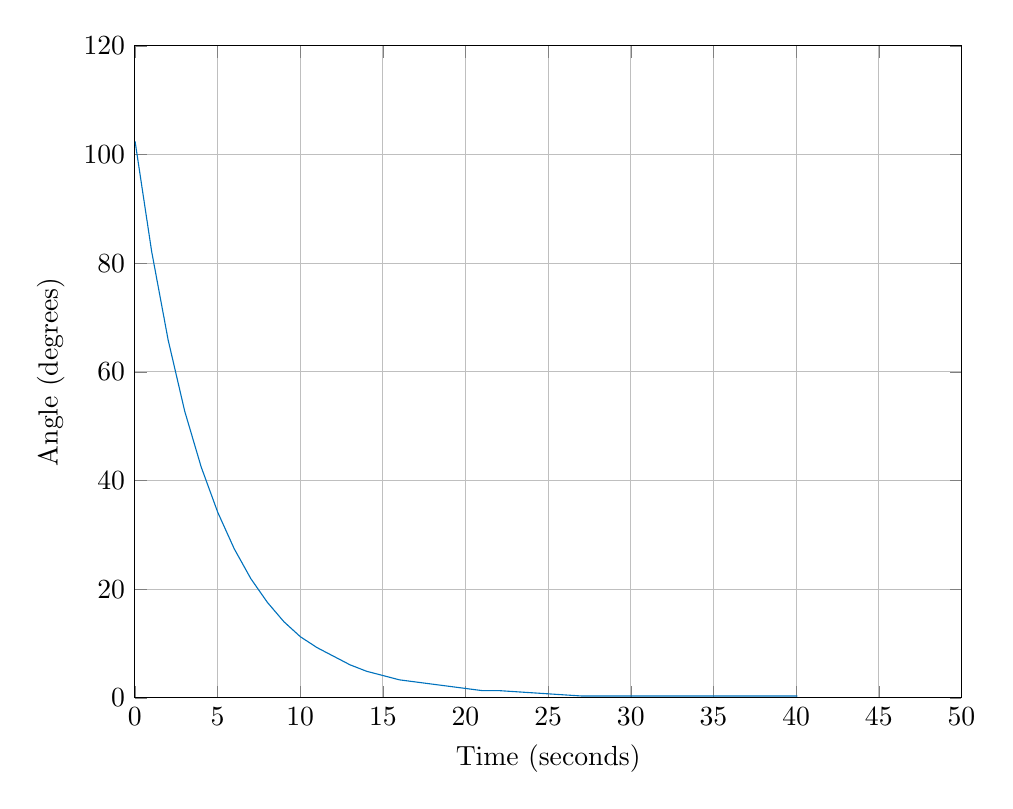
\begin{tikzpicture}

\begin{axis}[%
width=4.133in,
height=3.26in,
at={(0.693in,0.44in)},
scale only axis,
xmin=0,
xmax=50,
xmajorgrids,
xlabel={Time (seconds)},
ymin=0,
ymax=120,
ymajorgrids,
ylabel={Angle (degrees)},
axis background/.style={fill=white}
]
\addplot [color=mycolor1,solid,forget plot]
  table[row sep=crcr]{%
0	102.4204\\
0.0177441540000001	102.2904\\
0.0327040630000001	102.0084\\
0.0478449689999996	101.7024\\
0.0659545939999996	101.3764\\
0.080935841	101.0304\\
0.095923176	100.7244\\
0.11195197	100.3944\\
0.128055795	100.0804\\
0.143941748	99.7664\\
0.159967933999999	99.4424\\
0.176042313999999	99.1204\\
0.191954450999999	98.7984\\
0.208009254	98.4744\\
0.22399488	98.1384\\
0.239953013999999	97.8224\\
0.256054853999999	97.5004\\
0.272063669	97.1744\\
0.288027004	96.8584\\
0.303887813	96.5344\\
0.319971607	96.2124\\
0.335942635	95.8864\\
0.352025743	95.5644\\
0.3679568	95.2404\\
0.383953943	94.9204\\
0.399997912	94.5904\\
0.415998250999999	94.2584\\
0.431831394	93.9364\\
0.447814032000001	93.6144\\
0.463808589999999	93.2984\\
0.479903010999999	92.9684\\
0.495925008	92.6384\\
0.511948347	92.3244\\
0.528016396999999	92.0044\\
0.543863147999999	91.6824\\
0.562388751999999	91.3364\\
0.577608655	91.0044\\
0.592719001999999	90.6904\\
0.608161168000001	90.3764\\
0.624069551	90.0484\\
0.639885296999999	89.7304\\
0.655866359	89.4184\\
0.671987365999999	89.0844\\
0.68802496	88.7644\\
0.703813795999999	88.4404\\
0.719840768	88.1244\\
0.738192618	87.7884\\
0.753498854999999	87.4724\\
0.768784837	87.1484\\
0.784015643	86.8264\\
0.79988878	86.5084\\
0.815969871	86.1864\\
0.831983674	85.8584\\
0.848057242	85.5364\\
0.863854896999999	85.2164\\
0.879894759999999	84.8904\\
0.896003269	84.5704\\
0.911933238999999	84.2464\\
0.928035511999999	83.9184\\
0.943938683999999	83.5984\\
0.960191785999999	83.2744\\
0.975936873000001	82.9504\\
0.991975221	82.6244\\
1.007904933	82.2844\\
1.025398666	81.9884\\
1.040304124	81.7444\\
1.055833496	81.4964\\
1.07185873	81.2404\\
1.090013931	80.9524\\
1.10576894	80.6964\\
1.120861382	80.4444\\
1.13702896	80.1784\\
1.152233154	79.9104\\
1.167848246	79.6544\\
1.183945535	79.4024\\
1.199813575	79.1404\\
1.21810959	78.8724\\
1.233479532	78.6064\\
1.248819967	78.3504\\
1.264119629	78.0944\\
1.2799481	77.8364\\
1.29600457	77.5724\\
1.311980842	77.3024\\
1.327919031	77.0324\\
1.343886916	76.7824\\
1.362367992	76.5124\\
1.377645444	76.2584\\
1.392841231	76.0024\\
1.408078793	75.7424\\
1.424022405	75.4824\\
1.44007512	75.2244\\
1.456127821	74.9624\\
1.472010755	74.6984\\
1.488089533	74.4384\\
1.505276587	74.1684\\
1.52042763	73.9004\\
1.53601755	73.6464\\
1.551942352	73.3884\\
1.567911675	73.1324\\
1.583936325	72.8704\\
1.59989258	72.6104\\
1.615819365	72.3484\\
1.632013797	72.0864\\
1.647959463	71.8264\\
1.663988703	71.5504\\
1.679942628	71.2924\\
1.695987233	71.0364\\
1.712021079	70.7784\\
1.727901406	70.5184\\
1.743933763	70.2584\\
1.762257126	69.9884\\
1.777463037	69.7304\\
1.792770717	69.4624\\
1.808294613	69.2004\\
1.823994137	68.9484\\
1.839996003	68.6904\\
1.856026653	68.4284\\
1.87199263	68.1664\\
1.887955314	67.8964\\
1.903810895	67.6384\\
1.919953914	67.3844\\
1.937593507	67.1124\\
1.952661926	66.8484\\
1.968163942	66.5904\\
1.984178283	66.3324\\
1.999975183	66.0704\\
2.017791296	65.7864\\
2.033056711	65.5964\\
2.047987846	65.4004\\
2.063870266	65.1944\\
2.079834083	64.9804\\
2.096071024	64.7744\\
2.111796419	64.5704\\
2.128044492	64.3624\\
2.143898936	64.1504\\
2.162297373	63.9344\\
2.177444796	63.7284\\
2.192580046	63.5124\\
2.208046917	63.3064\\
2.223993811	63.1024\\
2.239942403	62.8964\\
2.255908685	62.6904\\
2.271844786	62.4784\\
2.290082946	62.2644\\
2.305663551	62.0484\\
2.321427334	61.8464\\
2.337415825	61.6344\\
2.353051482	61.4204\\
2.368230299	61.2164\\
2.384770288	61.0064\\
2.400381588	60.8004\\
2.416019773	60.5944\\
2.432075243	60.3864\\
2.447866992	60.1744\\
2.464034625	59.9684\\
2.479959588	59.7564\\
2.49605535	59.5484\\
2.511924627	59.3344\\
2.528096842	59.1224\\
2.543935965	58.9204\\
2.562280086	58.7044\\
2.577486766	58.4964\\
2.592615542	58.2884\\
2.607909968	58.0824\\
2.624013005	57.8764\\
2.639972317	57.6664\\
2.656019128	57.4564\\
2.671991098	57.2464\\
2.68783833	57.0384\\
2.70381914	56.8264\\
2.719797684	56.6184\\
2.735945271	56.4004\\
2.751977241	56.1984\\
2.767867978	55.9944\\
2.7839776	55.7844\\
2.799980396	55.5704\\
2.816165123	55.3624\\
2.832033263	55.1524\\
2.847985654	54.9444\\
2.864002992	54.7344\\
2.879987682	54.5264\\
2.895901791	54.3164\\
2.912123187	54.1064\\
2.928500747	53.8944\\
2.943946666	53.6764\\
2.959812605	53.4824\\
2.976001123	53.2704\\
2.991910687	53.0644\\
3.0078866	52.8424\\
3.024033743	52.6524\\
3.039833721	52.4944\\
3.055898507	52.3384\\
3.071898381	52.1744\\
3.088173756	52.0064\\
3.104241709	51.8384\\
3.119908618	51.6784\\
3.135877983	51.5124\\
3.151981441	51.3504\\
3.167814753	51.1824\\
3.184016414	51.0204\\
3.200035055	50.8524\\
3.215996707	50.6904\\
3.232054362	50.5204\\
3.247981445	50.3564\\
3.264166714	50.1904\\
3.279790125	50.0304\\
3.296012658	49.8644\\
3.311932396	49.7004\\
3.328156619	49.5344\\
3.343862637	49.3684\\
3.360331353	49.2044\\
3.376034386	49.0404\\
3.391958477	48.8744\\
3.407941351	48.7124\\
3.423828912	48.5464\\
3.442126699	48.3744\\
3.457365924	48.2124\\
3.472518824	48.0504\\
3.487868274	47.8844\\
3.503812755	47.7184\\
3.519945999	47.5484\\
3.536039249	47.3864\\
3.551938139	47.2284\\
3.568311326	47.0584\\
3.58398362	46.8904\\
3.599969341	46.7284\\
3.615951755	46.5644\\
3.63205545	46.4004\\
3.64796565	46.2344\\
3.665660884	46.0664\\
3.680830758	45.8984\\
3.696031371	45.7384\\
3.711993129	45.5684\\
3.728110995	45.4084\\
3.743985369	45.2424\\
3.760051875	45.0824\\
3.775931153	44.9184\\
3.792102727	44.7544\\
3.808065336	44.5884\\
3.823949485	44.4244\\
3.839914836	44.2564\\
3.856126292	44.0884\\
3.873129683	43.9244\\
3.888415745	43.7624\\
3.904082118	43.5984\\
3.919984447	43.4344\\
3.936797435	43.2664\\
3.95218989	43.0964\\
3.968030944	42.9344\\
3.983982969	42.7644\\
4.000019606	42.6004\\
4.01792116	42.4224\\
4.032913303	42.3104\\
4.047921539	42.1824\\
4.063861382	42.0524\\
4.079857392	41.9164\\
4.095891563	41.7824\\
4.111924659	41.6524\\
4.128192669	41.5204\\
4.143978449	41.3864\\
4.160134024	41.2524\\
4.175925001	41.1144\\
4.191796591	40.9824\\
4.208089832	40.8524\\
4.223946351	40.7204\\
4.239814982	40.5824\\
4.255999085	40.4524\\
4.271969471	40.3204\\
4.290295194	40.1804\\
4.305524384	40.0464\\
4.320741453	39.9204\\
4.335983263	39.7884\\
4.351886062	39.6544\\
4.368028138	39.5224\\
4.383969334	39.3824\\
4.399897934	39.2504\\
4.415925558	39.1204\\
4.431869626	38.9884\\
4.447996477	38.8524\\
4.46381962	38.7164\\
4.479957766	38.5884\\
4.495888877	38.4504\\
4.511978467	38.3144\\
4.527944261	38.1844\\
4.544003875	38.0524\\
4.560241184	37.9224\\
4.575958202	37.7904\\
4.592020126	37.6544\\
4.607920568	37.5244\\
4.624013937	37.3924\\
4.640030653	37.2584\\
4.655955594	37.1244\\
4.671990289	36.9924\\
4.688046214	36.8584\\
4.703806353	36.7224\\
4.719801313	36.5924\\
4.736013502	36.4564\\
4.751897951	36.3264\\
4.768033836	36.1924\\
4.784005832	36.0604\\
4.799899736	35.9244\\
4.815913036	35.7924\\
4.83196671	35.6584\\
4.847775381	35.5224\\
4.863984264	35.3944\\
4.879931643	35.2624\\
4.896051845	35.1244\\
4.911995762	34.9924\\
4.92815309	34.8604\\
4.94391307	34.7244\\
4.960371144	34.5904\\
4.975975883	34.4604\\
4.991936031	34.3284\\
5.00796669	34.1864\\
5.025225409	34.0624\\
5.040174419	33.9604\\
5.055830857	33.8544\\
5.071826165	33.7524\\
5.087915419	33.6364\\
5.103793775	33.5304\\
5.119982737	33.4224\\
5.13764764	33.3164\\
5.152925242	33.2104\\
5.168468381	33.0984\\
5.183880225	32.9964\\
5.199997693	32.8864\\
5.215913877	32.7764\\
5.231898023	32.6704\\
5.247995057	32.5644\\
5.2637976	32.4564\\
5.279791141	32.3464\\
5.296316409	32.2424\\
5.311987624	32.1284\\
5.328189245	32.0244\\
5.343948408	31.9164\\
5.359967983	31.8104\\
5.375954299	31.7044\\
5.391856128	31.5944\\
5.408098391	31.4864\\
5.424079379	31.3804\\
5.440023342	31.2724\\
5.456021868	31.1644\\
5.471990165	31.0544\\
5.488435392	30.9484\\
5.503975324	30.8384\\
5.519860487	30.7344\\
5.535996266	30.6244\\
5.552034071	30.5164\\
5.567791657	30.4084\\
5.583803568	30.3024\\
5.600058789	30.1884\\
5.615944598	30.0844\\
5.632002603	29.9744\\
5.647977485	29.8684\\
5.664107499	29.7604\\
5.679982405	29.6544\\
5.695809307	29.5444\\
5.711927927	29.4384\\
5.727864808	29.3324\\
5.743947707	29.2224\\
5.760158351	29.1144\\
5.775988783	29.0084\\
5.792046087	28.8964\\
5.808040178	28.7904\\
5.823975249	28.6844\\
5.839938834	28.5764\\
5.856000936	28.4684\\
5.871980058	28.3604\\
5.888114707	28.2524\\
5.903881931	28.1424\\
5.922154549	28.0324\\
5.935949996	27.9304\\
5.952079521	27.8244\\
5.967914484	27.7144\\
5.983887847	27.6044\\
6.00001967	27.4984\\
6.018431561	27.3744\\
6.033455699	27.2984\\
6.048482665	27.2164\\
6.063855193	27.1304\\
6.07987279	27.0424\\
6.095898001	26.9564\\
6.111976692	26.8724\\
6.128136278	26.7824\\
6.143940917	26.6964\\
6.159904689	26.6084\\
6.175983181	26.5184\\
6.191947174	26.4324\\
6.207838687	26.3444\\
6.224096146	26.2564\\
6.239995549	26.1684\\
6.256025953	26.0824\\
6.271936895	25.9964\\
6.2881028	25.9084\\
6.303821208	25.8204\\
6.319907718	25.7324\\
6.33602018	25.6444\\
6.351954771	25.5564\\
6.367979261	25.4684\\
6.383979535	25.3824\\
6.3999932	25.2964\\
6.415959658	25.2084\\
6.431813065	25.1204\\
6.44795526	25.0304\\
6.46633681	24.9404\\
6.481640492	24.8544\\
6.496800582	24.7684\\
6.512015123	24.6804\\
6.528007565	24.5924\\
6.544001335	24.5084\\
6.560166974	24.4204\\
6.575941672	24.3304\\
6.591818356	24.2444\\
6.607989749	24.1524\\
6.623906393	24.0664\\
6.64011637	23.9784\\
6.655979844	23.8944\\
6.673691636	23.8024\\
6.688914219	23.7144\\
6.704891777	23.6264\\
6.720183131	23.5424\\
6.737123565	23.4524\\
6.752308488	23.3684\\
6.768028357	23.2764\\
6.783980568	23.1964\\
6.799984341	23.1064\\
6.815967206	23.0164\\
6.83203869	22.9264\\
6.847972771	22.8404\\
6.864023079	22.7524\\
6.879902425	22.6664\\
6.895983262	22.5804\\
6.912068584	22.4904\\
6.928217671	22.4004\\
6.943979611	22.3184\\
6.960208831	22.2304\\
6.975958476	22.1444\\
6.992048525	22.0544\\
7.007884522	21.9604\\
7.025348728	21.8884\\
7.040294171	21.8204\\
7.055880966	21.7504\\
7.071901506	21.6824\\
7.08792888	21.6104\\
7.103913066	21.5404\\
7.120068382	21.4724\\
7.137139436	21.3984\\
7.152855242	21.3304\\
7.168165895	21.2624\\
7.183959671	21.1944\\
7.19999932	21.1264\\
7.215985663	21.0564\\
7.231883992	20.9824\\
7.247973186	20.9144\\
7.263937812	20.8464\\
7.280008721	20.7764\\
7.295851106	20.7064\\
7.312005332	20.6384\\
7.328187843	20.5684\\
7.343982595	20.4964\\
7.36024405	20.4244\\
7.375927101	20.3544\\
7.391989892	20.2844\\
7.4079011	20.2164\\
7.42401634	20.1464\\
7.440028795	20.0784\\
7.456084628	20.0064\\
7.471871999	19.9364\\
7.487989159	19.8644\\
7.504021292	19.7944\\
7.519989669	19.7284\\
7.536008014	19.6584\\
7.551949195	19.5904\\
7.567858875	19.5204\\
7.583935748	19.4484\\
7.601006903	19.3764\\
7.616333011	19.3084\\
7.631832045	19.2404\\
7.648012658	19.1724\\
7.66422105	19.1024\\
7.679991222	19.0304\\
7.695870973	18.9624\\
7.711873373	18.8924\\
7.728006439	18.8224\\
7.743939256	18.7524\\
7.76020953	18.6824\\
7.775971928	18.6104\\
7.792052602	18.5404\\
7.807974727	18.4704\\
7.823995777	18.4004\\
7.840030888	18.3344\\
7.855979139	18.2644\\
7.872011384	18.1944\\
7.8880804	18.1224\\
7.903981492	18.0544\\
7.920021161	17.9864\\
7.93706545	17.9124\\
7.952477327	17.8444\\
7.9678801	17.7764\\
7.983891723	17.7064\\
8.000016786	17.6364\\
8.017869878	17.5564\\
8.032826874	17.5104\\
8.047843233	17.4524\\
8.065963524	17.3984\\
8.080942145	17.3384\\
8.096041817	17.2824\\
8.112014951	17.2244\\
8.12803528	17.1684\\
8.14397842	17.1124\\
8.16001178	17.0544\\
8.176267969	17.0004\\
8.191914898	16.9404\\
8.207940751	16.8824\\
8.224000021	16.8284\\
8.240027206	16.7684\\
8.256005689	16.7104\\
8.272060388	16.6524\\
8.288060868	16.5984\\
8.30464051	16.5404\\
8.320066414	16.4824\\
8.335981801	16.4264\\
8.352041405	16.3684\\
8.367962458	16.3124\\
8.383991149	16.2544\\
8.399972366	16.1964\\
8.416015853	16.1384\\
8.432958448	16.0824\\
8.448360829	16.0264\\
8.463990804	15.9684\\
8.480266458	15.9124\\
8.495865174	15.8544\\
8.511956939	15.8004\\
8.527865723	15.7424\\
8.544168528	15.6844\\
8.559968157	15.6304\\
8.578390398	15.5684\\
8.593594679	15.5104\\
8.608849229	15.4604\\
8.624003037	15.4004\\
8.640080341	15.3424\\
8.655987797	15.2864\\
8.671984308	15.2284\\
8.687931107	15.1704\\
8.704159782	15.1144\\
8.719962013	15.0584\\
8.735946497	14.9984\\
8.752022388	14.9404\\
8.767927688	14.8864\\
8.783984821	14.8284\\
8.800003878	14.7724\\
8.816004223	14.7144\\
8.831966095	14.6584\\
8.848040975	14.6024\\
8.863999835	14.5424\\
8.880144963	14.4904\\
8.895806699	14.4304\\
8.912055063	14.3724\\
8.927921969	14.3124\\
8.944068836	14.2604\\
8.959911623	14.2024\\
8.978394041	14.1424\\
8.993690196	14.0844\\
9.008788051	14.0284\\
9.023814294	13.9764\\
9.041908105	13.9324\\
9.05681926	13.8904\\
9.071835365	13.8464\\
9.087841756	13.8044\\
9.103845233	13.7584\\
9.119976837	13.7104\\
9.136027025	13.6684\\
9.151993408	13.6244\\
9.167967223	13.5804\\
9.183994778	13.5344\\
9.199965717	13.4924\\
9.215891879	13.4484\\
9.231996951	13.4044\\
9.247892359	13.3584\\
9.263988631	13.3124\\
9.280002711	13.2704\\
9.295985623	13.2244\\
9.311957464	13.1804\\
9.327999411	13.1344\\
9.344179888	13.0924\\
9.360029036	13.0444\\
9.376214415	13.0024\\
9.392500602	12.9584\\
9.408018805	12.9124\\
9.423992344	12.8724\\
9.439977644	12.8244\\
9.455994021	12.7824\\
9.472021477	12.7344\\
9.488143487	12.6904\\
9.50406149	12.6444\\
9.519982771	12.6044\\
9.53603548	12.5584\\
9.552021988	12.5144\\
9.567994715	12.4724\\
9.584045985	12.4244\\
9.599980426	12.3824\\
9.616004284	12.3364\\
9.631946195	12.2924\\
9.648059476	12.2484\\
9.663985559	12.2024\\
9.679989567	12.1604\\
9.69599361	12.1144\\
9.711961915	12.0704\\
9.727990195	12.0244\\
9.744101561	11.9804\\
9.759973811	11.9364\\
9.778293465	11.8924\\
9.793577786	11.8484\\
9.808858878	11.8024\\
9.824244693	11.7624\\
9.840290734	11.7144\\
9.856116657	11.6724\\
9.872206048	11.6264\\
9.887930688	11.5824\\
9.903899309	11.5384\\
9.919951271	11.4944\\
9.935977203	11.4504\\
9.951984689	11.4044\\
9.967981481	11.3604\\
9.983956633	11.3104\\
9.999947442	11.2684\\
10.017871321	11.2244\\
10.032808961	11.1944\\
10.047859833	11.1644\\
10.063820433	11.1344\\
10.0819286	11.1004\\
10.09690558	11.0704\\
10.112008278	11.0364\\
10.127976725	11.0064\\
10.144209833	10.9744\\
10.159980776	10.9444\\
10.176072019	10.9124\\
10.192019298	10.8824\\
10.207919569	10.8504\\
10.223870053	10.8184\\
10.239996002	10.7844\\
10.25602208	10.7544\\
10.272043914	10.7224\\
10.28804911	10.6924\\
10.304009835	10.6604\\
10.319993903	10.6244\\
10.336057205	10.5944\\
10.352030243	10.5644\\
10.367956325	10.5324\\
10.384016425	10.5024\\
10.399949676	10.4704\\
10.415887273	10.4384\\
10.431963201	10.4044\\
10.448001658	10.3744\\
10.46402966	10.3404\\
10.480015026	10.3104\\
10.495952148	10.2764\\
10.511976326	10.2444\\
10.5279805	10.2144\\
10.544210234	10.1824\\
10.559986281	10.1504\\
10.575948973	10.1204\\
10.591905897	10.0884\\
10.608046685	10.0544\\
10.623974856	10.0244\\
10.639982006	9.99440000000001\\
10.656007648	9.9624\\
10.672016717	9.93040000000001\\
10.688027015	9.8984\\
10.703883115	9.86439999999999\\
10.719850408	9.8344\\
10.736036028	9.80439999999999\\
10.751966715	9.77239999999999\\
10.768060426	9.7424\\
10.784009615	9.7064\\
10.799861772	9.67439999999999\\
10.815977265	9.64439999999999\\
10.832009553	9.61239999999999\\
10.847977785	9.58240000000001\\
10.864036139	9.5504\\
10.88002107	9.5184\\
10.896019403	9.48439999999999\\
10.911838149	9.45039999999999\\
10.927964589	9.41839999999999\\
10.944132473	9.38839999999999\\
10.960012842	9.35639999999999\\
10.97599494	9.32640000000001\\
10.991880004	9.2944\\
11.007970899	9.26239999999999\\
11.025414481	9.23239999999998\\
11.040451894	9.2084\\
11.055869466	9.18640000000001\\
11.071919421	9.16040000000001\\
11.087924862	9.1344\\
11.103969424	9.1024\\
11.1199788	9.07639999999999\\
11.135877788	9.0504\\
11.151980131	9.02640000000001\\
11.167941124	9.00039999999998\\
11.183995078	8.97639999999998\\
11.200015884	8.95239999999998\\
11.215937089	8.9264\\
11.232019305	8.90040000000002\\
11.248020617	8.87639999999999\\
11.26421936	8.8484\\
11.280012	8.8244\\
11.296021746	8.79639999999999\\
11.312080644	8.77440000000001\\
11.328057691	8.74639999999999\\
11.344028408	8.72439999999999\\
11.360011019	8.69639999999998\\
11.376003706	8.6704\\
11.391936738	8.6464\\
11.407981734	8.62039999999999\\
11.424002395	8.59639999999999\\
11.440014917	8.57039999999999\\
11.45609619	8.54639999999999\\
11.472070065	8.5204\\
11.488103465	8.4944\\
11.5039031	8.4704\\
11.520077922	8.44439999999999\\
11.536003773	8.4164\\
11.551989733	8.39439999999999\\
11.567961579	8.3664\\
11.584026304	8.3424\\
11.599964638	8.31639999999999\\
11.615866219	8.2924\\
11.632051283	8.2664\\
11.648008565	8.24039999999999\\
11.663991783	8.21639999999999\\
11.679955904	8.19039999999998\\
11.695908896	8.1664\\
11.712044954	8.14039999999999\\
11.727984646	8.1144\\
11.744266289	8.09039999999997\\
11.760126251	8.06439999999999\\
11.7760434	8.0364\\
11.792132146	8.01439999999999\\
11.808050886	7.9864\\
11.823997807	7.9624\\
11.84004679	7.93639999999999\\
11.855996079	7.91040000000001\\
11.872030726	7.88639999999998\\
11.888012132	7.8604\\
11.90389773	7.83639999999998\\
11.919992051	7.80839999999999\\
11.935992807	7.78440000000001\\
11.95189877	7.75839999999998\\
11.967868711	7.7324\\
11.984037355	7.70639999999999\\
12.000105929	7.68039999999999\\
12.017849286	7.65440000000001\\
12.032768543	7.63239999999999\\
12.047866061	7.60639999999999\\
12.063880419	7.58039999999998\\
12.079877976	7.5564\\
12.098046519	7.5284\\
12.113407982	7.50639999999999\\
12.128578276	7.47839999999999\\
12.14398879	7.45439999999999\\
12.159980736	7.43039999999999\\
12.176133999	7.40440000000001\\
12.191915091	7.37639999999999\\
12.208001663	7.3544\\
12.224002396	7.32639999999999\\
12.239964929	7.30239999999999\\
12.255964619	7.27640000000001\\
12.272018179	7.25039999999998\\
12.287907709	7.22639999999998\\
12.303960852	7.20039999999999\\
12.319980397	7.1764\\
12.335941135	7.1484\\
12.351983059	7.12439999999999\\
12.367987037	7.0984\\
12.384113476	7.0744\\
12.400041719	7.04639999999999\\
12.416061042	7.02440000000001\\
12.431941691	6.99639999999999\\
12.447990776	6.97239999999999\\
12.46400612	6.94639999999998\\
12.47986539	6.9224\\
12.496005331	6.8964\\
12.511977477	6.8724\\
12.527990866	6.84639999999999\\
12.544075412	6.82039999999999\\
12.560051507	6.79639999999999\\
12.576208672	6.7704\\
12.591987399	6.7444\\
12.607988185	6.7204\\
12.623998292	6.69439999999999\\
12.640042872	6.6664\\
12.655954371	6.64439999999999\\
12.671993002	6.6144\\
12.688069214	6.5924\\
12.704052035	6.56439999999999\\
12.720157683	6.5424\\
12.735883019	6.5164\\
12.751988071	6.49039999999999\\
12.767953513	6.46639999999999\\
12.784022603	6.44039999999998\\
12.79994475	6.4144\\
12.815851826	6.39039999999999\\
12.831979317	6.3644\\
12.848006828	6.33639999999998\\
12.864024507	6.3124\\
12.879993846	6.2864\\
12.896013505	6.26039999999999\\
12.912028027	6.2364\\
12.927939231	6.2124\\
12.94406223	6.18639999999999\\
12.959992479	6.16040000000001\\
12.978385834	6.13639999999998\\
12.993673517	6.10839999999999\\
13.008884356	6.08039999999998\\
13.023873171	6.0624\\
13.039965823	6.0424\\
13.055962863	6.02440000000001\\
13.072056005	6.00839999999999\\
13.088051354	5.99039999999999\\
13.103908324	5.9704\\
13.119826742	5.94839999999999\\
13.135977399	5.93039999999999\\
13.151916194	5.91240000000001\\
13.168070177	5.89239999999998\\
13.18398576	5.8724\\
13.199890941	5.8524\\
13.215990689	5.83439999999999\\
13.231990683	5.81439999999999\\
13.248005491	5.8004\\
13.263988195	5.78040000000001\\
13.280023099	5.76039999999999\\
13.295914622	5.74039999999999\\
13.3120289	5.72239999999999\\
13.327973192	5.70239999999998\\
13.3463917	5.68039999999999\\
13.361635521	5.66240000000001\\
13.376936742	5.64239999999998\\
13.392542949	5.62439999999999\\
13.407984984	5.60839999999999\\
13.423990415	5.58839999999998\\
13.440035161	5.57039999999999\\
13.456027312	5.5504\\
13.472029757	5.53240000000001\\
13.488019035	5.51239999999999\\
13.504048668	5.4924\\
13.519997101	5.47239999999999\\
13.535957424	5.45239999999998\\
13.551978436	5.4344\\
13.567960935	5.4204\\
13.583982097	5.40040000000002\\
13.600088893	5.38039999999998\\
13.616051723	5.3604\\
13.632095198	5.3404\\
13.647936911	5.32239999999999\\
13.664018976	5.30239999999999\\
13.679929405	5.28240000000001\\
13.696115557	5.26239999999999\\
13.712088791	5.2444\\
13.728079724	5.22439999999999\\
13.744146188	5.21040000000001\\
13.760004076	5.19039999999998\\
13.776138129	5.1704\\
13.791990433	5.15040000000002\\
13.808319523	5.13239999999999\\
13.823991519	5.11239999999999\\
13.840876282	5.0924\\
13.856198395	5.07239999999999\\
13.872022927	5.0544\\
13.88799893	5.0364\\
13.903902853	5.01839999999999\\
13.920299171	5.00039999999998\\
13.936524143	4.9804\\
13.952003133	4.96040000000001\\
13.967922164	4.94239999999999\\
13.984021356	4.9224\\
14.000004302	4.90240000000001\\
14.021512803	4.88239999999999\\
14.033500279	4.8724\\
14.048825728	4.8604\\
14.064094519	4.8484\\
14.079982062	4.8344\\
14.096036069	4.8244\\
14.111978945	4.81039999999999\\
14.127970598	4.79639999999999\\
14.144272802	4.78440000000001\\
14.159927968	4.77239999999999\\
14.176001765	4.76039999999999\\
14.191993996	4.74839999999999\\
14.208044255	4.73439999999999\\
14.224030353	4.7204\\
14.239899612	4.71040000000001\\
14.25595932	4.6964\\
14.271973075	4.6844\\
14.28807093	4.6704\\
14.303881156	4.66040000000001\\
14.319956078	4.64439999999999\\
14.337491235	4.63239999999999\\
14.352804817	4.62039999999999\\
14.368146496	4.60839999999999\\
14.384045512	4.59439999999999\\
14.399862218	4.58239999999998\\
14.415813551	4.57039999999999\\
14.431962165	4.55839999999999\\
14.447932542	4.5444\\
14.464199591	4.53040000000001\\
14.47987596	4.5204\\
14.496005858	4.5044\\
14.511931121	4.4944\\
14.527984224	4.4804\\
14.543959983	4.4684\\
14.559920262	4.45439999999999\\
14.576162621	4.44239999999999\\
14.591981038	4.43039999999999\\
14.608046856	4.41839999999999\\
14.62399606	4.40440000000001\\
14.640035955	4.39039999999999\\
14.655874969	4.38039999999998\\
14.67200585	4.3664\\
14.687913297	4.3544\\
14.703887227	4.3404\\
14.720035739	4.33039999999998\\
14.736084322	4.31440000000001\\
14.751996589	4.30439999999999\\
14.767982716	4.29040000000001\\
14.784021955	4.2784\\
14.799951995	4.26439999999999\\
14.815974284	4.25239999999999\\
14.832722157	4.24039999999999\\
14.848035872	4.22839999999999\\
14.86398905	4.2144\\
14.880026604	4.20039999999999\\
14.896024939	4.19039999999998\\
14.912215675	4.1764\\
14.927989651	4.1644\\
14.943997957	4.15040000000002\\
14.959906851	4.14039999999999\\
14.978305886	4.12439999999999\\
14.99354199	4.11239999999999\\
15.008697568	4.0984\\
15.023974395	4.0844\\
15.039986789	4.0744\\
15.056140917	4.06039999999999\\
15.072027932	4.0504\\
15.087898911	4.0384\\
15.104072529	4.02439999999999\\
15.119999799	4.01039999999999\\
15.136014341	4.00039999999998\\
15.151948685	3.98439999999999\\
15.16794009	3.97439999999999\\
15.183979463	3.96040000000001\\
15.200022249	3.94839999999999\\
15.215902045	3.9344\\
15.231979085	3.9224\\
15.24810982	3.9084\\
15.26400462	3.89840000000001\\
15.279983627	3.8844\\
15.296015789	3.87039999999999\\
15.311988997	3.8604\\
15.327958147	3.84639999999999\\
15.344116503	3.8344\\
15.359944198	3.81839999999998\\
15.375985619	3.8064\\
15.391964544	3.79040000000001\\
15.407926139	3.78040000000001\\
15.423929022	3.7684\\
15.440027877	3.75439999999999\\
15.4559316	3.74039999999999\\
15.471922784	3.7304\\
15.487959992	3.71639999999999\\
15.503849215	3.70439999999999\\
15.522218674	3.68839999999999\\
15.537355028	3.6784\\
15.552485878	3.6664\\
15.567856399	3.65240000000001\\
15.583983553	3.64039999999999\\
15.599907845	3.62839999999998\\
15.615964183	3.6164\\
15.631958534	3.60040000000001\\
15.64799247	3.59039999999997\\
15.663977415	3.57839999999999\\
15.679929334	3.56439999999999\\
15.695828736	3.5504\\
15.712003932	3.54040000000001\\
15.72812514	3.52640000000001\\
15.744129129	3.51239999999999\\
15.759839239	3.50039999999998\\
15.776051962	3.4884\\
15.791962243	3.4764\\
15.807942971	3.46039999999998\\
15.824014363	3.45039999999999\\
15.840027182	3.43839999999999\\
15.855982539	3.42440000000001\\
15.872008117	3.41040000000001\\
15.887972795	3.40040000000002\\
15.903826785	3.38839999999998\\
15.919920663	3.3724\\
15.935967355	3.3604\\
15.95200946	3.3484\\
15.967943705	3.33639999999998\\
15.983972538	3.32239999999999\\
15.999983157	3.3124\\
16.018615015	3.29839999999999\\
16.031993003	3.29639999999999\\
16.048060554	3.2884\\
16.064007484	3.28240000000001\\
16.079901392	3.2784\\
16.095854435	3.2704\\
16.111999047	3.26239999999999\\
16.128037352	3.25839999999999\\
16.144240554	3.25039999999998\\
16.159954101	3.2424\\
16.175951184	3.2384\\
16.191984654	3.2324\\
16.207904056	3.2264\\
16.223985031	3.2204\\
16.240024681	3.2124\\
16.25600208	3.2084\\
16.272006995	3.20039999999999\\
16.288044368	3.19239999999999\\
16.304065686	3.18839999999999\\
16.319995551	3.18039999999999\\
16.335958025	3.1724\\
16.352009455	3.16839999999999\\
16.367880078	3.16240000000001\\
16.38399931	3.1584\\
16.399958407	3.15040000000002\\
16.415849514	3.14239999999998\\
16.431883881	3.13839999999999\\
16.447992115	3.13039999999998\\
16.464002217	3.1224\\
16.480128507	3.11839999999999\\
16.495935629	3.1104\\
16.511965451	3.10639999999999\\
16.527942849	3.0984\\
16.544002784	3.0924\\
16.559951852	3.08840000000001\\
16.576310388	3.08039999999998\\
16.591993916	3.07239999999999\\
16.607981093	3.0684\\
16.624099508	3.06039999999999\\
16.639977816	3.05239999999999\\
16.655957981	3.04839999999999\\
16.672075781	3.0424\\
16.687981617	3.0364\\
16.70408034	3.03040000000001\\
16.720016419	3.02239999999999\\
16.7359338	3.01839999999999\\
16.752928353	3.01039999999999\\
16.768076001	3.00239999999999\\
16.784042128	2.99839999999999\\
16.799941782	2.99039999999999\\
16.816403911	2.98440000000001\\
16.831945972	2.97839999999999\\
16.848033424	2.97239999999999\\
16.86404063	2.96639999999999\\
16.880056043	2.96040000000001\\
16.89597555	2.95239999999998\\
16.911809413	2.94839999999999\\
16.927964491	2.94039999999998\\
16.943859189	2.9324\\
16.959847547	2.9284\\
16.976306144	2.9204\\
16.991895648	2.9144\\
17.007861192	2.9084\\
17.023903461	2.90240000000001\\
17.039888521	2.8964\\
17.055981314	2.89039999999999\\
17.071804681	2.88239999999999\\
17.08812132	2.87839999999998\\
17.103986067	2.87039999999999\\
17.11994946	2.86239999999999\\
17.135943308	2.85839999999999\\
17.152028495	2.8524\\
17.167997112	2.84439999999999\\
17.183813738	2.8404\\
17.1999706	2.83239999999998\\
17.216001494	2.82839999999999\\
17.231945523	2.82039999999999\\
17.248143254	2.8124\\
17.263959356	2.80839999999999\\
17.279957697	2.8004\\
17.295903573	2.7924\\
17.311831899	2.7884\\
17.327913376	2.78240000000001\\
17.34387256	2.7764\\
17.360021005	2.7704\\
17.376265783	2.76239999999999\\
17.392021055	2.75839999999999\\
17.407958846	2.75039999999998\\
17.424052004	2.7424\\
17.440041537	2.7384\\
17.455980248	2.7304\\
17.47205077	2.72239999999999\\
17.487902924	2.7184\\
17.503972557	2.7124\\
17.519909292	2.7064\\
17.535974259	2.70039999999999\\
17.551906023	2.69239999999999\\
17.567973181	2.68839999999999\\
17.583989841	2.68039999999999\\
17.599989014	2.6724\\
17.615818706	2.66839999999999\\
17.631799887	2.66040000000001\\
17.64796211	2.65240000000001\\
17.66402742	2.64840000000001\\
17.680030102	2.64239999999998\\
17.695854282	2.63839999999999\\
17.711905321	2.63039999999998\\
17.727900065	2.6224\\
17.744114573	2.61839999999999\\
17.75999217	2.6104\\
17.776111038	2.6024\\
17.791797316	2.5984\\
17.808062441	2.5924\\
17.823913438	2.58439999999999\\
17.840021682	2.58039999999998\\
17.855995502	2.57239999999999\\
17.872057927	2.5684\\
17.88793406	2.56039999999999\\
17.90402632	2.55239999999999\\
17.919969605	2.54839999999999\\
17.936015152	2.54040000000001\\
17.952047514	2.53240000000001\\
17.967998953	2.5284\\
17.98408643	2.5204\\
17.999937903	2.51439999999999\\
18.017713904	2.51039999999999\\
18.032926989	2.50239999999999\\
18.048076682	2.49839999999999\\
18.063924107	2.49039999999999\\
18.080003085	2.4824\\
18.096008291	2.47839999999999\\
18.111842246	2.4704\\
18.130062683	2.4624\\
18.145491549	2.4584\\
18.160759238	2.45039999999999\\
18.175956101	2.4464\\
18.191884821	2.43839999999999\\
18.20806147	2.4324\\
18.224692697	2.4284\\
18.239952728	2.4204\\
18.256008258	2.41240000000001\\
18.272024733	2.4084\\
18.288010349	2.40040000000002\\
18.30410588	2.39239999999998\\
18.320001355	2.38839999999999\\
18.335972967	2.38239999999999\\
18.351979796	2.37839999999998\\
18.36816057	2.37039999999999\\
18.383868069	2.36239999999999\\
18.400025477	2.35839999999999\\
18.416136989	2.35040000000001\\
18.431947889	2.3424\\
18.447949276	2.33840000000001\\
18.463946043	2.33239999999998\\
18.479997801	2.32639999999999\\
18.496050152	2.32039999999999\\
18.511806667	2.3124\\
18.527798792	2.30639999999998\\
18.543893029	2.3004\\
18.559880903	2.2924\\
18.576054051	2.2884\\
18.591822555	2.28040000000001\\
18.607864675	2.27239999999999\\
18.623982842	2.26839999999999\\
18.640034433	2.26239999999999\\
18.655940578	2.2564\\
18.671970701	2.24839999999999\\
18.688088237	2.2424\\
18.704055742	2.2384\\
18.719847187	2.2304\\
18.735947129	2.22239999999999\\
18.751992392	2.2184\\
18.767902927	2.21040000000001\\
18.783831042	2.20239999999998\\
18.7999934	2.19839999999999\\
18.815810661	2.19239999999999\\
18.834114914	2.18639999999999\\
18.84946709	2.18039999999999\\
18.864867929	2.1724\\
18.880255113	2.16839999999999\\
18.895962589	2.16040000000001\\
18.911859012	2.15240000000001\\
18.927977997	2.14840000000001\\
18.943940977	2.14039999999999\\
18.959923903	2.13439999999999\\
18.976041518	2.12839999999998\\
18.991981506	2.1224\\
19.007935539	2.1164\\
19.025572889	2.10839999999999\\
19.040871928	2.1024\\
19.056438628	2.0984\\
19.072266862	2.0904\\
19.087987123	2.08239999999998\\
19.104017448	2.07839999999999\\
19.120041113	2.07039999999999\\
19.136089582	2.06439999999999\\
19.152001241	2.05839999999999\\
19.167970653	2.05239999999999\\
19.183993411	2.04839999999999\\
19.19997326	2.04040000000001\\
19.217370569	2.03240000000001\\
19.232709265	2.0284\\
19.248086704	2.0204\\
19.263974539	2.01239999999999\\
19.280053441	2.00839999999999\\
19.295960011	2.00239999999999\\
19.311846466	1.99639999999999\\
19.330104587	1.99039999999999\\
19.345462389	1.9824\\
19.36091123	1.97839999999999\\
19.376104842	1.9704\\
19.391941061	1.9624\\
19.407895005	1.9584\\
19.424153682	1.95039999999999\\
19.439978196	1.94239999999999\\
19.455975314	1.93839999999999\\
19.472029896	1.9324\\
19.487922857	1.92639999999999\\
19.50403235	1.9204\\
19.519984596	1.91240000000001\\
19.536018948	1.9084\\
19.552021052	1.90040000000002\\
19.567933364	1.89239999999998\\
19.584057507	1.88839999999999\\
19.599982401	1.88039999999998\\
19.616378024	1.8724\\
19.631959547	1.86839999999999\\
19.647867944	1.86239999999999\\
19.663884525	1.85839999999999\\
19.680028676	1.85040000000001\\
19.69598001	1.8424\\
19.711797359	1.83840000000001\\
19.729901931	1.83039999999998\\
19.745080392	1.82239999999999\\
19.760194592	1.8184\\
19.77598209	1.81039999999999\\
19.791910871	1.80639999999998\\
19.808114813	1.8004\\
19.823910719	1.7924\\
19.839977941	1.7884\\
19.856102042	1.78040000000001\\
19.872069051	1.77239999999999\\
19.887886331	1.76839999999999\\
19.904063416	1.76039999999999\\
19.919879187	1.75239999999999\\
19.935990063	1.74839999999999\\
19.952153276	1.74039999999999\\
19.967911568	1.7364\\
19.984041665	1.72839999999999\\
19.999969177	1.72239999999999\\
20.017754685	1.71639999999999\\
20.033065576	1.71040000000001\\
20.048261028	1.70239999999998\\
20.065148395	1.69839999999999\\
20.080584776	1.69039999999998\\
20.095921297	1.6824\\
20.112314658	1.6784\\
20.128072212	1.6724\\
20.144050322	1.6644\\
20.160008674	1.66040000000001\\
20.176244886	1.65240000000001\\
20.191946088	1.64840000000001\\
20.208192053	1.64039999999999\\
20.223937571	1.63239999999999\\
20.240101997	1.62839999999998\\
20.255949027	1.62039999999999\\
20.272073862	1.6144\\
20.288048639	1.60839999999999\\
20.303961711	1.6024\\
20.320062529	1.5984\\
20.336051327	1.5904\\
20.351867158	1.58239999999998\\
20.367998558	1.57839999999999\\
20.384235131	1.57039999999999\\
20.399970861	1.5624\\
20.416047321	1.55839999999999\\
20.432002035	1.5504\\
20.447985038	1.5444\\
20.463823328	1.5384\\
20.479886681	1.53240000000001\\
20.495986982	1.5284\\
20.511926494	1.5204\\
20.527922729	1.51239999999999\\
20.543957572	1.50839999999999\\
20.559990106	1.50039999999998\\
20.575967763	1.4924\\
20.592058742	1.4884\\
20.60784029	1.4824\\
20.623964623	1.4764\\
20.639915171	1.4684\\
20.655942033	1.4624\\
20.672022121	1.4584\\
20.687986574	1.45039999999999\\
20.707530295	1.44239999999999\\
20.7198142	1.43839999999999\\
20.735799943	1.43039999999999\\
20.754076883	1.4224\\
20.769131774	1.41839999999999\\
20.785242884	1.41040000000001\\
20.800413404	1.4064\\
20.815900959	1.40040000000002\\
20.831911751	1.39239999999998\\
20.847991349	1.38839999999999\\
20.864215246	1.38039999999998\\
20.880172489	1.3724\\
20.89604119	1.36839999999999\\
20.912091578	1.3604\\
20.927945847	1.3544\\
20.944081173	1.3484\\
20.960066684	1.3424\\
20.975969002	1.33840000000001\\
20.991931671	1.33039999999998\\
21.007976778	1.3244\\
21.025607157	1.32239999999999\\
21.041084259	1.32239999999999\\
21.056381035	1.32239999999999\\
21.071975516	1.32239999999999\\
21.08800851	1.32239999999999\\
21.104036106	1.32239999999999\\
21.11978888	1.32239999999999\\
21.136058816	1.32239999999999\\
21.151994684	1.32239999999999\\
21.167953509	1.32239999999999\\
21.184001052	1.32239999999999\\
21.199977548	1.32239999999999\\
21.215797052	1.32239999999999\\
21.234055508	1.32239999999999\\
21.249365023	1.32239999999999\\
21.264517231	1.32239999999999\\
21.280016451	1.32239999999999\\
21.295960836	1.32239999999999\\
21.311862378	1.32239999999999\\
21.327983413	1.32239999999999\\
21.34406115	1.32239999999999\\
21.359918185	1.32239999999999\\
21.375870588	1.32239999999999\\
21.391958276	1.32239999999999\\
21.408024456	1.32239999999999\\
21.423858845	1.32239999999999\\
21.439904702	1.32239999999999\\
21.455890771	1.32239999999999\\
21.472065636	1.32239999999999\\
21.487990324	1.32239999999999\\
21.503924697	1.32239999999999\\
21.519952902	1.32239999999999\\
21.536053434	1.32239999999999\\
21.552156546	1.32239999999999\\
21.567988841	1.32239999999999\\
21.583994477	1.32239999999999\\
21.59996743	1.32239999999999\\
21.615992246	1.32239999999999\\
21.655064028	1.32239999999999\\
21.670173849	1.32239999999999\\
21.686191848	1.32239999999999\\
21.702176256	1.32239999999999\\
21.718242571	1.32239999999999\\
21.734196731	1.32239999999999\\
21.752411665	1.32239999999999\\
21.767800269	1.32239999999999\\
21.783079991	1.32239999999999\\
21.798362695	1.32239999999999\\
21.814357483	1.32239999999999\\
21.830303609	1.32239999999999\\
21.846278672	1.32239999999999\\
21.862192804	1.32239999999999\\
21.880667552	1.32239999999999\\
21.895776652	1.32239999999999\\
21.910926669	1.32239999999999\\
21.926283994	1.32239999999999\\
21.944665708	1.32239999999999\\
21.959741178	1.32239999999999\\
21.974922207	1.32239999999999\\
21.990247147	1.32239999999999\\
22.006397717	1.32239999999999\\
22.023988324	1.32239999999999\\
22.039055139	1.32039999999999\\
22.05430491	1.3164\\
22.070331314	1.31440000000001\\
22.086381205	1.3124\\
22.102324425	1.30839999999999\\
22.11844384	1.30439999999999\\
22.134320397	1.30239999999999\\
22.150300566	1.29839999999999\\
22.166279265	1.2944\\
22.182322897	1.2924\\
22.198249003	1.2884\\
22.214245136	1.28440000000001\\
22.230301005	1.28240000000001\\
22.246394786	1.2784\\
22.262230523	1.27439999999999\\
22.278448973	1.27239999999999\\
22.294239367	1.26839999999999\\
22.310426027	1.26639999999999\\
22.326201298	1.26239999999999\\
22.342466703	1.26039999999999\\
22.358312833	1.2564\\
22.374320144	1.2544\\
22.390375329	1.25239999999999\\
22.406225986	1.24639999999999\\
22.422235792	1.2444\\
22.438465649	1.2424\\
22.454329415	1.2384\\
22.470383371	1.23439999999999\\
22.486352676	1.2324\\
22.502240175	1.22839999999999\\
22.518396709	1.2244\\
22.534244035	1.22239999999999\\
22.550249363	1.2184\\
22.566291798	1.2144\\
22.582415262	1.2124\\
22.5984103	1.2084\\
22.614325262	1.20439999999999\\
22.630270806	1.20239999999998\\
22.64632788	1.20239999999998\\
22.662287485	1.1964\\
22.680877012	1.1944\\
22.696397841	1.19239999999999\\
22.711552355	1.18639999999999\\
22.726574298	1.1844\\
22.742327242	1.1824\\
22.758279839	1.1784\\
22.774478613	1.17439999999999\\
22.790305551	1.1724\\
22.806395373	1.16839999999999\\
22.822354675	1.1644\\
22.838466497	1.16240000000001\\
22.854355785	1.1584\\
22.870407877	1.15440000000001\\
22.88631445	1.15240000000001\\
22.902387617	1.14840000000001\\
22.918459556	1.14439999999999\\
22.934269089	1.14239999999998\\
22.950361492	1.13839999999999\\
22.96629014	1.13639999999999\\
22.982346792	1.1344\\
22.998236221	1.13239999999999\\
23.019628587	1.12639999999999\\
23.031469793	1.12439999999999\\
23.046564953	1.1224\\
23.062298764	1.1164\\
23.078402653	1.1144\\
23.094178311	1.11239999999999\\
23.110200395	1.10839999999999\\
23.127454235	1.1044\\
23.143406326	1.1024\\
23.158732463	1.0984\\
23.174360877	1.09439999999999\\
23.190324647	1.0924\\
23.206298972	1.08840000000001\\
23.222169591	1.0844\\
23.238559523	1.08240000000001\\
23.254371491	1.07839999999999\\
23.270249796	1.0744\\
23.286372482	1.07239999999999\\
23.302282086	1.07239999999999\\
23.318186828	1.0664\\
23.334156421	1.06440000000001\\
23.350343948	1.0624\\
23.366284072	1.0564\\
23.382328887	1.05439999999999\\
23.398255897	1.05239999999999\\
23.414166942	1.04839999999999\\
23.430330648	1.0444\\
23.446383868	1.0424\\
23.462191018	1.0384\\
23.478430311	1.03440000000001\\
23.494241708	1.03240000000001\\
23.510470816	1.0284\\
23.526358042	1.02439999999999\\
23.542700745	1.02239999999999\\
23.558199073	1.01839999999999\\
23.574375386	1.01439999999999\\
23.590330593	1.01239999999999\\
23.606500598	1.00839999999999\\
23.622688537	1.0064\\
23.638185474	1.00239999999999\\
23.654196095	1.00239999999999\\
23.670408415	0.996399999999994\\
23.686326759	0.994399999999999\\
23.702264482	0.992400000000004\\
23.718290795	0.986400000000003\\
23.734374509	0.984399999999994\\
23.750286653	0.982399999999998\\
23.766291469	0.978399999999993\\
23.78234744	0.974400000000003\\
23.798177011	0.972399999999993\\
23.814320352	0.968400000000003\\
23.830228216	0.964399999999998\\
23.846288473	0.962400000000002\\
23.862190859	0.958399999999997\\
23.878302401	0.954399999999993\\
23.894256324	0.952399999999983\\
23.910209326	0.948399999999992\\
23.928327762	0.946399999999997\\
23.943538498	0.942399999999992\\
23.958722043	0.940399999999997\\
23.974378754	0.936399999999992\\
23.990177182	0.932400000000001\\
24.00855221	0.932400000000001\\
24.022871924	0.926399999999987\\
24.038509697	0.924399999999991\\
24.054292439	0.922399999999996\\
24.070268278	0.918399999999991\\
24.086144764	0.914400000000001\\
24.102335473	0.912400000000005\\
24.118289543	0.9084\\
24.134209088	0.90440000000001\\
24.150364932	0.902400000000014\\
24.16630243	0.898400000000009\\
24.18243555	0.89439999999999\\
24.198321486	0.892399999999981\\
24.214354372	0.88839999999999\\
24.230180066	0.884399999999999\\
24.246290664	0.88239999999999\\
24.262274475	0.878399999999985\\
24.278342243	0.87639999999999\\
24.294426776	0.874399999999994\\
24.310343148	0.872399999999999\\
24.326225234	0.866399999999999\\
24.342217303	0.864400000000003\\
24.360546942	0.862399999999994\\
24.375647749	0.856399999999994\\
24.390990519	0.854399999999998\\
24.406294182	0.852400000000003\\
24.422268531	0.848399999999998\\
24.438308004	0.844399999999993\\
24.454332951	0.842399999999998\\
24.470233269	0.838400000000007\\
24.486268323	0.834400000000002\\
24.502342485	0.832400000000007\\
24.518159415	0.828399999999988\\
24.534170077	0.824399999999997\\
24.550332823	0.822399999999988\\
24.56636199	0.818399999999997\\
24.582348102	0.816400000000002\\
24.598328392	0.812399999999997\\
24.61425054	0.812399999999997\\
24.630282536	0.806399999999996\\
24.646314333	0.804399999999987\\
24.66241766	0.802399999999992\\
24.678344394	0.796399999999991\\
24.69437882	0.794399999999996\\
24.710248503	0.792400000000001\\
24.726220501	0.788399999999996\\
24.742386991	0.784400000000005\\
24.758171706	0.78240000000001\\
24.774276598	0.778400000000005\\
24.790359155	0.774399999999986\\
24.806220989	0.77239999999999\\
24.822354658	0.768399999999986\\
24.838330041	0.764399999999995\\
24.854223247	0.762399999999985\\
24.870422163	0.758399999999995\\
24.886866671	0.754400000000004\\
24.902317714	0.752399999999994\\
24.918228638	0.74839999999999\\
24.934330968	0.746399999999994\\
24.950296628	0.742400000000004\\
24.966439927	0.742400000000004\\
24.982181905	0.736400000000003\\
24.998338685	0.734399999999994\\
25.019140482	0.732399999999998\\
25.031151038	0.726399999999998\\
25.04632837	0.724400000000003\\
25.062254328	0.722399999999993\\
25.07828592	0.718400000000003\\
25.094461408	0.714399999999998\\
25.110176998	0.712400000000002\\
25.126163718	0.708399999999997\\
25.142242643	0.704399999999993\\
25.158240413	0.702399999999983\\
25.174292944	0.698399999999992\\
25.19017162	0.694400000000002\\
25.206191876	0.692399999999992\\
25.222269787	0.688399999999987\\
25.238238855	0.684399999999997\\
25.256529852	0.682400000000001\\
25.272086529	0.680399999999992\\
25.28706972	0.676399999999987\\
25.302328479	0.674399999999991\\
25.318327917	0.672399999999996\\
25.334252533	0.666399999999996\\
25.350385947	0.664400000000001\\
25.366357627	0.662400000000005\\
25.382352689	0.656400000000005\\
25.398467113	0.65440000000001\\
25.414221319	0.652400000000014\\
25.430408024	0.648400000000009\\
25.446212433	0.64439999999999\\
25.464439046	0.642399999999981\\
25.479621267	0.63839999999999\\
25.49472912	0.634399999999999\\
25.510384383	0.63239999999999\\
25.526536748	0.628399999999985\\
25.542392689	0.624399999999994\\
25.558391582	0.622399999999999\\
25.574182136	0.618399999999994\\
25.590396774	0.616399999999999\\
25.606315667	0.612399999999994\\
25.622186452	0.612399999999994\\
25.638168271	0.606399999999994\\
25.654182391	0.604399999999998\\
25.670203463	0.602400000000003\\
25.686304702	0.596399999999988\\
25.702142729	0.594399999999993\\
25.720392975	0.592399999999998\\
25.735504011	0.586399999999998\\
25.750497624	0.584400000000002\\
25.766330907	0.582400000000007\\
25.782142986	0.578399999999988\\
25.800180284	0.574399999999997\\
25.815242579	0.572399999999988\\
25.830473416	0.568399999999997\\
25.846232104	0.564400000000006\\
25.862354178	0.562399999999997\\
25.878265906	0.558399999999992\\
25.894347376	0.556399999999996\\
25.91036042	0.552399999999992\\
25.926333271	0.550399999999996\\
25.942327844	0.546399999999991\\
25.958210236	0.544399999999996\\
25.976436178	0.542400000000001\\
25.991580363	0.5364\\
26.006959245	0.534400000000005\\
26.024235248	0.53240000000001\\
26.039267488	0.52640000000001\\
26.054277042	0.524399999999986\\
26.070167825	0.52239999999999\\
26.086260823	0.518399999999986\\
26.102151778	0.514399999999995\\
26.118181712	0.512399999999985\\
26.13432692	0.508399999999995\\
26.150200076	0.504400000000004\\
26.1663409	0.502399999999994\\
26.182296298	0.49839999999999\\
26.198312342	0.494399999999999\\
26.214310844	0.492400000000004\\
26.230265631	0.488399999999999\\
26.2462289	0.486400000000003\\
26.262379877	0.482399999999998\\
26.278300511	0.482399999999998\\
26.294359329	0.476399999999998\\
26.310370588	0.474400000000003\\
26.326516458	0.472399999999993\\
26.342636789	0.466399999999993\\
26.358333657	0.464399999999998\\
26.374295671	0.462400000000002\\
26.39031626	0.458399999999997\\
26.406390167	0.454399999999993\\
26.422336635	0.452399999999983\\
26.438388681	0.448399999999992\\
26.454356703	0.444400000000002\\
26.470336431	0.442399999999992\\
26.486230453	0.438399999999987\\
26.502330661	0.434399999999997\\
26.518147054	0.432400000000001\\
26.53417113	0.428399999999996\\
26.550368614	0.426399999999987\\
26.566345426	0.422399999999996\\
26.582350471	0.420400000000001\\
26.598330385	0.416399999999996\\
26.623998244	0.414400000000001\\
26.630175521	0.412400000000005\\
26.646173326	0.406400000000005\\
26.662223168	0.40440000000001\\
26.678223535	0.402400000000014\\
26.694342251	0.398400000000009\\
26.71034016	0.39439999999999\\
26.726521206	0.392399999999981\\
26.74244475	0.38839999999999\\
26.758373091	0.384399999999999\\
26.774301207	0.38239999999999\\
26.79029648	0.378399999999985\\
26.806365657	0.374399999999994\\
26.822282652	0.372399999999999\\
26.838361476	0.368399999999994\\
26.854343001	0.364400000000003\\
26.870395761	0.362399999999994\\
26.886328543	0.358399999999989\\
26.902260285	0.356399999999994\\
26.918198218	0.354399999999998\\
26.934154711	0.352400000000003\\
26.950352974	0.346399999999988\\
26.966294747	0.344399999999993\\
26.982275437	0.342399999999998\\
26.998444123	0.336399999999998\\
27.019333815	0.334400000000002\\
27.031206463	0.332400000000007\\
27.046472644	0.330399999999997\\
27.062339693	0.330399999999997\\
27.078343179	0.330399999999997\\
27.094539878	0.330399999999997\\
27.110444733	0.330399999999997\\
27.126414222	0.330399999999997\\
27.142344233	0.330399999999997\\
27.158330115	0.330399999999997\\
27.174293356	0.330399999999997\\
27.190432098	0.330399999999997\\
27.206248855	0.330399999999997\\
27.222432874	0.330399999999997\\
27.238301631	0.330399999999997\\
27.254303991	0.330399999999997\\
27.270635766	0.330399999999997\\
27.286277598	0.330399999999997\\
27.302338254	0.330399999999997\\
27.318165342	0.330399999999997\\
27.334359687	0.330399999999997\\
27.35033754	0.330399999999997\\
27.366170499	0.330399999999997\\
27.382330342	0.330399999999997\\
27.398309848	0.330399999999997\\
27.414380358	0.330399999999997\\
27.430488232	0.330399999999997\\
27.44643189	0.330399999999997\\
27.462370393	0.330399999999997\\
27.478288669	0.330399999999997\\
27.496720725	0.330399999999997\\
27.511956949	0.330399999999997\\
27.527137468	0.330399999999997\\
27.54240456	0.330399999999997\\
27.558355809	0.330399999999997\\
27.574328803	0.330399999999997\\
27.590349212	0.330399999999997\\
27.606358677	0.330399999999997\\
27.622280033	0.330399999999997\\
27.638364331	0.330399999999997\\
27.654446103	0.330399999999997\\
27.670268076	0.330399999999997\\
27.686173776	0.330399999999997\\
27.719030526	0.330399999999997\\
27.735075717	0.330399999999997\\
27.751093501	0.330399999999997\\
27.767049159	0.330399999999997\\
27.783097455	0.330399999999997\\
27.799098514	0.330399999999997\\
27.815250921	0.330399999999997\\
27.831271767	0.330399999999997\\
27.847312228	0.330399999999997\\
27.863131055	0.330399999999997\\
27.879213798	0.330399999999997\\
27.895208294	0.330399999999997\\
27.911220526	0.330399999999997\\
27.927194339	0.330399999999997\\
27.9431723	0.330399999999997\\
27.959520713	0.330399999999997\\
27.975158815	0.330399999999997\\
27.991204791	0.330399999999997\\
28.007168107	0.330399999999997\\
28.024759165	0.330399999999997\\
28.03916397	0.330399999999997\\
28.055328858	0.330399999999997\\
28.071123681	0.330399999999997\\
28.087179867	0.330399999999997\\
28.103215152	0.330399999999997\\
28.119020403	0.330399999999997\\
28.137149918	0.330399999999997\\
28.152357627	0.330399999999997\\
28.167548669	0.330399999999997\\
28.183226684	0.330399999999997\\
28.199257532	0.330399999999997\\
28.215214795	0.330399999999997\\
28.231215865	0.330399999999997\\
28.247136926	0.330399999999997\\
28.263180299	0.330399999999997\\
28.279120863	0.330399999999997\\
28.295228677	0.330399999999997\\
28.311224629	0.330399999999997\\
28.327183392	0.330399999999997\\
28.343277864	0.330399999999997\\
28.359190185	0.330399999999997\\
28.3752436	0.330399999999997\\
28.391272344	0.330399999999997\\
28.40713285	0.330399999999997\\
28.423215148	0.330399999999997\\
28.439229806	0.330399999999997\\
28.455096114	0.330399999999997\\
28.471240582	0.330399999999997\\
28.487312208	0.330399999999997\\
28.503094577	0.330399999999997\\
28.519025287	0.330399999999997\\
28.53504709	0.330399999999997\\
28.55119733	0.330399999999997\\
28.567215089	0.330399999999997\\
28.583237694	0.330399999999997\\
28.599130151	0.330399999999997\\
28.615188817	0.330399999999997\\
28.631219034	0.330399999999997\\
28.647134746	0.330399999999997\\
28.663187656	0.330399999999997\\
28.679140584	0.330399999999997\\
28.695153261	0.330399999999997\\
28.711199465	0.330399999999997\\
28.727282942	0.330399999999997\\
28.743135156	0.330399999999997\\
28.759504863	0.330399999999997\\
28.775167797	0.330399999999997\\
28.791215195	0.330399999999997\\
28.807197627	0.330399999999997\\
28.823235199	0.330399999999997\\
28.839171798	0.330399999999997\\
28.855274927	0.330399999999997\\
28.871322067	0.330399999999997\\
28.887087775	0.330399999999997\\
28.903315521	0.330399999999997\\
28.919172491	0.330399999999997\\
28.935137292	0.330399999999997\\
28.95115737	0.330399999999997\\
28.967286687	0.330399999999997\\
28.983093588	0.330399999999997\\
28.99921377	0.330399999999997\\
29.020118709	0.330399999999997\\
29.032143043	0.330399999999997\\
29.04743031	0.330399999999997\\
29.063237173	0.330399999999997\\
29.079186787	0.330399999999997\\
29.09521026	0.330399999999997\\
29.111259421	0.330399999999997\\
29.127156918	0.330399999999997\\
29.143218523	0.330399999999997\\
29.15930211	0.330399999999997\\
29.175217517	0.330399999999997\\
29.19122775	0.330399999999997\\
29.207224717	0.330399999999997\\
29.223212618	0.330399999999997\\
29.239281804	0.330399999999997\\
29.255377284	0.330399999999997\\
29.271270126	0.330399999999997\\
29.287193641	0.330399999999997\\
29.303207456	0.330399999999997\\
29.319215696	0.330399999999997\\
29.33522306	0.330399999999997\\
29.351245555	0.330399999999997\\
29.367110493	0.330399999999997\\
29.383232739	0.330399999999997\\
29.399274843	0.330399999999997\\
29.415114943	0.330399999999997\\
29.431206031	0.330399999999997\\
29.447206987	0.330399999999997\\
29.463189241	0.330399999999997\\
29.479206619	0.330399999999997\\
29.495190478	0.330399999999997\\
29.51119154	0.330399999999997\\
29.52958329	0.330399999999997\\
29.544659521	0.330399999999997\\
29.559801903	0.330399999999997\\
29.575254682	0.330399999999997\\
29.591209629	0.330399999999997\\
29.607026912	0.330399999999997\\
29.625414226	0.330399999999997\\
29.640730807	0.330399999999997\\
29.655994353	0.330399999999997\\
29.671139312	0.330399999999997\\
29.687224587	0.330399999999997\\
29.703031675	0.330399999999997\\
29.719074687	0.330399999999997\\
29.735237349	0.330399999999997\\
29.75123185	0.330399999999997\\
29.76724116	0.330399999999997\\
29.783195079	0.330399999999997\\
29.799303985	0.330399999999997\\
29.815245557	0.330399999999997\\
29.831318362	0.330399999999997\\
29.847186559	0.330399999999997\\
29.86317547	0.330399999999997\\
29.879152447	0.330399999999997\\
29.895281118	0.330399999999997\\
29.911228848	0.330399999999997\\
29.927216077	0.330399999999997\\
29.943234113	0.330399999999997\\
29.959540115	0.330399999999997\\
29.977023485	0.330399999999997\\
29.992197578	0.330399999999997\\
30.007443899	0.330399999999997\\
30.02484184	0.330399999999997\\
30.04003791	0.330399999999997\\
30.055263753	0.330399999999997\\
30.071304876	0.330399999999997\\
30.087284849	0.330399999999997\\
30.103217907	0.330399999999997\\
30.119249873	0.330399999999997\\
30.135153627	0.330399999999997\\
30.151063444	0.330399999999997\\
30.167217592	0.330399999999997\\
30.183298259	0.330399999999997\\
30.199232869	0.330399999999997\\
30.215176395	0.330399999999997\\
30.231212958	0.330399999999997\\
30.247380221	0.330399999999997\\
30.263170617	0.330399999999997\\
30.279236067	0.330399999999997\\
30.29524439	0.330399999999997\\
30.311189433	0.330399999999997\\
30.329670975	0.330399999999997\\
30.344985235	0.330399999999997\\
30.360344327	0.330399999999997\\
30.375516236	0.330399999999997\\
30.391363579	0.330399999999997\\
30.407215568	0.330399999999997\\
30.423240823	0.330399999999997\\
30.439305985	0.330399999999997\\
30.455232388	0.330399999999997\\
30.471254166	0.330399999999997\\
30.487148531	0.330399999999997\\
30.505375119	0.330399999999997\\
30.520681111	0.330399999999997\\
30.536056068	0.330399999999997\\
30.551319635	0.330399999999997\\
30.567217745	0.330399999999997\\
30.583058304	0.330399999999997\\
30.599221912	0.330399999999997\\
30.615259079	0.330399999999997\\
30.631271805	0.330399999999997\\
30.647229989	0.330399999999997\\
30.663458166	0.330399999999997\\
30.679151412	0.330399999999997\\
30.695233676	0.330399999999997\\
30.711058887	0.330399999999997\\
30.727045985	0.330399999999997\\
30.75490632	0.330399999999997\\
30.763624625	0.330399999999997\\
30.775545112	0.330399999999997\\
30.791088079	0.330399999999997\\
30.807297415	0.330399999999997\\
30.825937383	0.330399999999997\\
30.839252786	0.330399999999997\\
30.855233205	0.330399999999997\\
30.871216978	0.330399999999997\\
30.887219999	0.330399999999997\\
30.903235975	0.330399999999997\\
30.919210786	0.330399999999997\\
30.935233757	0.330399999999997\\
30.951213231	0.330399999999997\\
30.967235358	0.330399999999997\\
30.983188431	0.330399999999997\\
30.999216774	0.330399999999997\\
31.017936925	0.330399999999997\\
31.033276264	0.330399999999997\\
31.04868307	0.330399999999997\\
31.064165665	0.330399999999997\\
31.079514664	0.330399999999997\\
31.095351714	0.330399999999997\\
31.111034839	0.330399999999997\\
31.127148068	0.330399999999997\\
31.143199096	0.330399999999997\\
31.159345436	0.330399999999997\\
31.175212348	0.330399999999997\\
31.191184266	0.330399999999997\\
31.207252758	0.330399999999997\\
31.223225039	0.330399999999997\\
31.239134144	0.330399999999997\\
31.255560974	0.330399999999997\\
31.27107972	0.330399999999997\\
31.287171758	0.330399999999997\\
31.303247139	0.330399999999997\\
31.319209483	0.330399999999997\\
31.335190363	0.330399999999997\\
31.351095654	0.330399999999997\\
31.367107767	0.330399999999997\\
31.38320764	0.330399999999997\\
31.399308458	0.330399999999997\\
31.415100041	0.330399999999997\\
31.431041635	0.330399999999997\\
31.447188292	0.330399999999997\\
31.463090824	0.330399999999997\\
31.479182738	0.330399999999997\\
31.495294445	0.330399999999997\\
31.51151139	0.330399999999997\\
31.527134786	0.330399999999997\\
31.54319205	0.330399999999997\\
31.559301783	0.330399999999997\\
31.57521718	0.330399999999997\\
31.591226806	0.330399999999997\\
31.607193407	0.330399999999997\\
31.623235537	0.330399999999997\\
31.639127693	0.330399999999997\\
31.655226272	0.330399999999997\\
31.671139659	0.330399999999997\\
31.687317576	0.330399999999997\\
31.703727255	0.330399999999997\\
31.71931342	0.330399999999997\\
31.735231352	0.330399999999997\\
31.751460681	0.330399999999997\\
31.767177218	0.330399999999997\\
31.783250798	0.330399999999997\\
31.799188046	0.330399999999997\\
31.815097946	0.330399999999997\\
31.831226044	0.330399999999997\\
31.847192508	0.330399999999997\\
31.863226095	0.330399999999997\\
31.879218741	0.330399999999997\\
31.89519377	0.330399999999997\\
31.911405468	0.330399999999997\\
31.927253908	0.330399999999997\\
31.94306244	0.330399999999997\\
31.961186856	0.330399999999997\\
31.976265233	0.330399999999997\\
31.991262475	0.330399999999997\\
32.007106942	0.330399999999997\\
32.023086773	0.330399999999997\\
32.040123036	0.330399999999997\\
32.055169901	0.330399999999997\\
32.072137629	0.330399999999997\\
32.0874407	0.330399999999997\\
32.103262105	0.330399999999997\\
32.119194896	0.330399999999997\\
32.135386945	0.330399999999997\\
32.151092181	0.330399999999997\\
32.167208169	0.330399999999997\\
32.183211738	0.330399999999997\\
32.199146512	0.330399999999997\\
32.215208201	0.330399999999997\\
32.231292085	0.330399999999997\\
32.247191556	0.330399999999997\\
32.263443431	0.330399999999997\\
32.279232602	0.330399999999997\\
32.295248191	0.330399999999997\\
32.311183728	0.330399999999997\\
32.327478378	0.330399999999997\\
32.343077303	0.330399999999997\\
32.361332649	0.330399999999997\\
32.376582879	0.330399999999997\\
32.391757437	0.330399999999997\\
32.407194879	0.330399999999997\\
32.423214848	0.330399999999997\\
32.439124963	0.330399999999997\\
32.455197697	0.330399999999997\\
32.471265824	0.330399999999997\\
32.487209442	0.330399999999997\\
32.503224575	0.330399999999997\\
32.519233875	0.330399999999997\\
32.535158323	0.330399999999997\\
32.551172274	0.330399999999997\\
32.567180032	0.330399999999997\\
32.583173024	0.330399999999997\\
32.599204038	0.330399999999997\\
32.615132213	0.330399999999997\\
32.631098545	0.330399999999997\\
32.647192409	0.330399999999997\\
32.663191144	0.330399999999997\\
32.679227085	0.330399999999997\\
32.6952052	0.330399999999997\\
32.711143344	0.330399999999997\\
32.729500091	0.330399999999997\\
32.744513165	0.330399999999997\\
32.759539263	0.330399999999997\\
32.775207626	0.330399999999997\\
32.791199561	0.330399999999997\\
32.807195471	0.330399999999997\\
32.823221008	0.330399999999997\\
32.839163371	0.330399999999997\\
32.855247773	0.330399999999997\\
32.871125538	0.330399999999997\\
32.887075249	0.330399999999997\\
32.903204758	0.330399999999997\\
32.91926143	0.330399999999997\\
32.935307191	0.330399999999997\\
32.951015976	0.330399999999997\\
32.967257161	0.330399999999997\\
32.983177449	0.330399999999997\\
32.999117823	0.330399999999997\\
33.019708912	0.330399999999997\\
33.031909219	0.330399999999997\\
33.047157611	0.330399999999997\\
33.06329919	0.330399999999997\\
33.079236412	0.330399999999997\\
33.095301152	0.330399999999997\\
33.111168161	0.330399999999997\\
33.127168115	0.330399999999997\\
33.143177294	0.330399999999997\\
33.159231912	0.330399999999997\\
33.175238791	0.330399999999997\\
33.191148286	0.330399999999997\\
33.207191502	0.330399999999997\\
33.223148084	0.330399999999997\\
33.239197123	0.330399999999997\\
33.255254432	0.330399999999997\\
33.271248523	0.330399999999997\\
33.287132325	0.330399999999997\\
33.303012558	0.330399999999997\\
33.319194402	0.330399999999997\\
33.336278392	0.330399999999997\\
33.351614657	0.330399999999997\\
33.367209669	0.330399999999997\\
33.38321703	0.330399999999997\\
33.399228705	0.330399999999997\\
33.415229065	0.330399999999997\\
33.431115787	0.330399999999997\\
33.447066858	0.330399999999997\\
33.463234675	0.330399999999997\\
33.479182601	0.330399999999997\\
33.495243241	0.330399999999997\\
33.511190462	0.330399999999997\\
33.52720028	0.330399999999997\\
33.543161293	0.330399999999997\\
33.559288861	0.330399999999997\\
33.57522214	0.330399999999997\\
33.591434937	0.330399999999997\\
33.607181045	0.330399999999997\\
33.623055903	0.330399999999997\\
33.639136389	0.330399999999997\\
33.655141329	0.330399999999997\\
33.671188462	0.330399999999997\\
33.6871993	0.330399999999997\\
33.703194253	0.330399999999997\\
33.719135754	0.330399999999997\\
33.735302091	0.330399999999997\\
33.75119174	0.330399999999997\\
33.76724738	0.330399999999997\\
33.783180552	0.330399999999997\\
33.799264316	0.330399999999997\\
33.815229093	0.330399999999997\\
33.831251766	0.330399999999997\\
33.847175021	0.330399999999997\\
33.863193742	0.330399999999997\\
33.879208034	0.330399999999997\\
33.895280831	0.330399999999997\\
33.911174354	0.330399999999997\\
33.927170923	0.330399999999997\\
33.943106751	0.330399999999997\\
33.959648437	0.330399999999997\\
33.975230517	0.330399999999997\\
33.991201768	0.330399999999997\\
34.007225265	0.330399999999997\\
34.023222999	0.330399999999997\\
34.039175882	0.330399999999997\\
34.055188211	0.330399999999997\\
34.071081528	0.330399999999997\\
34.087106735	0.330399999999997\\
34.103100954	0.330399999999997\\
34.119098409	0.330399999999997\\
34.135229929	0.330399999999997\\
34.151222745	0.330399999999997\\
34.167213216	0.330399999999997\\
34.183185033	0.330399999999997\\
34.1992214	0.330399999999997\\
34.215192177	0.330399999999997\\
34.231204916	0.330399999999997\\
34.247181682	0.330399999999997\\
34.263217206	0.330399999999997\\
34.279091705	0.330399999999997\\
34.295123132	0.330399999999997\\
34.311066915	0.330399999999997\\
34.327177317	0.330399999999997\\
34.343150722	0.330399999999997\\
34.359554808	0.330399999999997\\
34.375179128	0.330399999999997\\
34.391439307	0.330399999999997\\
34.407238897	0.330399999999997\\
34.423211659	0.330399999999997\\
34.439151848	0.330399999999997\\
34.45522414	0.330399999999997\\
34.471226633	0.330399999999997\\
34.487521779	0.330399999999997\\
34.504042131	0.330399999999997\\
34.519242467	0.330399999999997\\
34.535038696	0.330399999999997\\
34.551232704	0.330399999999997\\
34.568065239	0.330399999999997\\
34.583299633	0.330399999999997\\
34.599265004	0.330399999999997\\
34.61515069	0.330399999999997\\
34.631103709	0.330399999999997\\
34.647090459	0.330399999999997\\
34.663186455	0.330399999999997\\
34.679111155	0.330399999999997\\
34.695245145	0.330399999999997\\
34.711187882	0.330399999999997\\
34.727187576	0.330399999999997\\
34.74313923	0.330399999999997\\
34.759209599	0.330399999999997\\
34.77511124	0.330399999999997\\
34.791212739	0.330399999999997\\
34.807119582	0.330399999999997\\
34.823238468	0.330399999999997\\
34.841180343	0.330399999999997\\
34.856305315	0.330399999999997\\
34.871586259	0.330399999999997\\
34.887160582	0.330399999999997\\
34.903177082	0.330399999999997\\
34.919096027	0.330399999999997\\
34.935017989	0.330399999999997\\
34.951161368	0.330399999999997\\
34.967187576	0.330399999999997\\
34.983199367	0.330399999999997\\
34.999482799	0.330399999999997\\
35.017804618	0.330399999999997\\
35.033079344	0.330399999999997\\
35.048396625	0.330399999999997\\
35.063661243	0.330399999999997\\
35.079158414	0.330399999999997\\
35.095285085	0.330399999999997\\
35.111119608	0.330399999999997\\
35.127151644	0.330399999999997\\
35.143158142	0.330399999999997\\
35.159198339	0.330399999999997\\
35.175137384	0.330399999999997\\
35.191338264	0.330399999999997\\
35.208322638	0.330399999999997\\
35.223728255	0.330399999999997\\
35.239592221	0.330399999999997\\
35.255289981	0.330399999999997\\
35.271205471	0.330399999999997\\
35.287114276	0.330399999999997\\
35.303649387	0.330399999999997\\
35.319197648	0.330399999999997\\
35.335226151	0.330399999999997\\
35.351078606	0.330399999999997\\
35.367044199	0.330399999999997\\
35.383196987	0.330399999999997\\
35.399216809	0.330399999999997\\
35.415244358	0.330399999999997\\
35.431091256	0.330399999999997\\
35.447062766	0.330399999999997\\
35.463219448	0.330399999999997\\
35.47908068	0.330399999999997\\
35.495182951	0.330399999999997\\
35.511222335	0.330399999999997\\
35.527173355	0.330399999999997\\
35.543316155	0.330399999999997\\
35.559639384	0.330399999999997\\
35.575198504	0.330399999999997\\
35.59122146	0.330399999999997\\
35.607569969	0.330399999999997\\
35.623469566	0.330399999999997\\
35.639107458	0.330399999999997\\
35.655228853	0.330399999999997\\
35.671233703	0.330399999999997\\
35.687326712	0.330399999999997\\
35.703202268	0.330399999999997\\
35.719206338	0.330399999999997\\
35.735022195	0.330399999999997\\
35.753222758	0.330399999999997\\
35.768438077	0.330399999999997\\
35.783778456	0.330399999999997\\
35.799171746	0.330399999999997\\
35.815167965	0.330399999999997\\
35.83194962	0.330399999999997\\
35.847232735	0.330399999999997\\
35.863199428	0.330399999999997\\
35.879206895	0.330399999999997\\
35.895300004	0.330399999999997\\
35.911271428	0.330399999999997\\
35.927566031	0.330399999999997\\
35.943183336	0.330399999999997\\
35.959414867	0.330399999999997\\
35.975147063	0.330399999999997\\
35.991219752	0.330399999999997\\
36.007352256	0.330399999999997\\
36.024779358	0.330399999999997\\
36.040551491	0.330399999999997\\
36.055934442	0.330399999999997\\
36.071329533	0.330399999999997\\
36.087304964	0.330399999999997\\
36.103243023	0.330399999999997\\
36.119230205	0.330399999999997\\
36.135265001	0.330399999999997\\
36.151137185	0.330399999999997\\
36.167179937	0.330399999999997\\
36.183167136	0.330399999999997\\
36.19940755	0.330399999999997\\
36.215169158	0.330399999999997\\
36.231280009	0.330399999999997\\
36.247116974	0.330399999999997\\
36.263288529	0.330399999999997\\
36.279168924	0.330399999999997\\
36.295182733	0.330399999999997\\
36.311108908	0.330399999999997\\
36.327529318	0.330399999999997\\
36.343222829	0.330399999999997\\
36.359271504	0.330399999999997\\
36.375156846	0.330399999999997\\
36.391285697	0.330399999999997\\
36.407330559	0.330399999999997\\
36.423259764	0.330399999999997\\
36.439224771	0.330399999999997\\
36.455291211	0.330399999999997\\
36.471268854	0.330399999999997\\
36.487173096	0.330399999999997\\
36.503204631	0.330399999999997\\
36.519191896	0.330399999999997\\
36.535268016	0.330399999999997\\
36.551125773	0.330399999999997\\
36.567043569	0.330399999999997\\
36.585259912	0.330399999999997\\
36.600439488	0.330399999999997\\
36.615815221	0.330399999999997\\
36.631160241	0.330399999999997\\
36.647177341	0.330399999999997\\
36.663309915	0.330399999999997\\
36.679227914	0.330399999999997\\
36.69528616	0.330399999999997\\
36.711190026	0.330399999999997\\
36.727305536	0.330399999999997\\
36.743228165	0.330399999999997\\
36.759265064	0.330399999999997\\
36.775105435	0.330399999999997\\
36.791200584	0.330399999999997\\
36.807170526	0.330399999999997\\
36.823209653	0.330399999999997\\
36.839250669	0.330399999999997\\
36.855106536	0.330399999999997\\
36.871273585	0.330399999999997\\
36.887381248	0.330399999999997\\
36.903220477	0.330399999999997\\
36.919249337	0.330399999999997\\
36.935025912	0.330399999999997\\
36.951020243	0.330399999999997\\
36.96942626	0.330399999999997\\
36.984628147	0.330399999999997\\
36.999939441	0.330399999999997\\
37.017880241	0.330399999999997\\
37.033216261	0.330399999999997\\
37.048572061	0.330399999999997\\
37.063790655	0.330399999999997\\
37.079175586	0.330399999999997\\
37.095204157	0.330399999999997\\
37.111223387	0.330399999999997\\
37.12734016	0.330399999999997\\
37.14322605	0.330399999999997\\
37.159120556	0.330399999999997\\
37.175225728	0.330399999999997\\
37.191195138	0.330399999999997\\
37.207101735	0.330399999999997\\
37.223213178	0.330399999999997\\
37.239058385	0.330399999999997\\
37.256299226	0.330399999999997\\
37.272137574	0.330399999999997\\
37.287187913	0.330399999999997\\
37.303135983	0.330399999999997\\
37.319206145	0.330399999999997\\
37.335270049	0.330399999999997\\
37.351231686	0.330399999999997\\
37.367178579	0.330399999999997\\
37.383244009	0.330399999999997\\
37.39919839	0.330399999999997\\
37.415234465	0.330399999999997\\
37.431226791	0.330399999999997\\
37.447122743	0.330399999999997\\
37.463164076	0.330399999999997\\
37.479134414	0.330399999999997\\
37.495172443	0.330399999999997\\
37.511093386	0.330399999999997\\
37.527177348	0.330399999999997\\
37.543180558	0.330399999999997\\
37.559477856	0.330399999999997\\
37.575317562	0.330399999999997\\
37.591262391	0.330399999999997\\
37.60719626	0.330399999999997\\
37.623245471	0.330399999999997\\
37.639265851	0.330399999999997\\
37.655168529	0.330399999999997\\
37.671218433	0.330399999999997\\
37.687210541	0.330399999999997\\
37.703224233	0.330399999999997\\
37.719202542	0.330399999999997\\
37.735034481	0.330399999999997\\
37.753180578	0.330399999999997\\
37.768418624	0.330399999999997\\
37.783697515	0.330399999999997\\
37.799247264	0.330399999999997\\
37.815180572	0.330399999999997\\
37.831222766	0.330399999999997\\
37.847186083	0.330399999999997\\
37.863219162	0.330399999999997\\
37.879082708	0.330399999999997\\
37.895143546	0.330399999999997\\
37.913441498	0.330399999999997\\
37.928658288	0.330399999999997\\
37.94403082	0.330399999999997\\
37.959500247	0.330399999999997\\
37.975113736	0.330399999999997\\
37.991129836	0.330399999999997\\
38.007210473	0.330399999999997\\
38.023525513	0.330399999999997\\
38.039149108	0.330399999999997\\
38.055198953	0.330399999999997\\
38.071218888	0.330399999999997\\
38.087340177	0.330399999999997\\
38.103117937	0.330399999999997\\
38.119184718	0.330399999999997\\
38.137056201	0.330399999999997\\
38.152367187	0.330399999999997\\
38.167674254	0.330399999999997\\
38.183225546	0.330399999999997\\
38.1990744	0.330399999999997\\
38.215159114	0.330399999999997\\
38.232041016	0.330399999999997\\
38.247298418	0.330399999999997\\
38.26314307	0.330399999999997\\
38.279145896	0.330399999999997\\
38.295161073	0.330399999999997\\
38.311234653	0.330399999999997\\
38.327284701	0.330399999999997\\
38.343162625	0.330399999999997\\
38.361571079	0.330399999999997\\
38.376743353	0.330399999999997\\
38.391865865	0.330399999999997\\
38.407215851	0.330399999999997\\
38.423154854	0.330399999999997\\
38.439193463	0.330399999999997\\
38.455212941	0.330399999999997\\
38.471225792	0.330399999999997\\
38.487191359	0.330399999999997\\
38.503242545	0.330399999999997\\
38.519189664	0.330399999999997\\
38.535251669	0.330399999999997\\
38.551195877	0.330399999999997\\
38.567220934	0.330399999999997\\
38.583194252	0.330399999999997\\
38.599252838	0.330399999999997\\
38.615190871	0.330399999999997\\
38.631229939	0.330399999999997\\
38.647128343	0.330399999999997\\
38.663115006	0.330399999999997\\
38.679209966	0.330399999999997\\
38.695140503	0.330399999999997\\
38.711084157	0.330399999999997\\
38.727551114	0.330399999999997\\
38.743176295	0.330399999999997\\
38.759470772	0.330399999999997\\
38.775213597	0.330399999999997\\
38.791224191	0.330399999999997\\
38.807190649	0.330399999999997\\
38.823259885	0.330399999999997\\
38.839066351	0.330399999999997\\
38.857467284	0.330399999999997\\
38.872944038	0.330399999999997\\
38.888385762	0.330399999999997\\
38.903732644	0.330399999999997\\
38.919272102	0.330399999999997\\
38.935090382	0.330399999999997\\
38.951088628	0.330399999999997\\
38.967189332	0.330399999999997\\
38.983010976	0.330399999999997\\
38.999097872	0.330399999999997\\
39.019867301	0.330399999999997\\
39.031849222	0.330399999999997\\
39.047223634	0.330399999999997\\
39.063298625	0.330399999999997\\
39.079086305	0.330399999999997\\
39.095257725	0.330399999999997\\
39.111102294	0.330399999999997\\
39.127299192	0.330399999999997\\
39.143130494	0.330399999999997\\
39.1592026	0.330399999999997\\
39.175120408	0.330399999999997\\
39.19122053	0.330399999999997\\
39.207161224	0.330399999999997\\
39.223153746	0.330399999999997\\
39.239235439	0.330399999999997\\
39.255078353	0.330399999999997\\
39.27123874	0.330399999999997\\
39.287348372	0.330399999999997\\
39.303170695	0.330399999999997\\
39.319202881	0.330399999999997\\
39.335328885	0.330399999999997\\
39.351138102	0.330399999999997\\
39.367312281	0.330399999999997\\
39.383178742	0.330399999999997\\
39.399098282	0.330399999999997\\
39.415155863	0.330399999999997\\
39.431244924	0.330399999999997\\
39.447200037	0.330399999999997\\
39.463237155	0.330399999999997\\
39.479176336	0.330399999999997\\
39.495259927	0.330399999999997\\
39.51118298	0.330399999999997\\
39.527164279	0.330399999999997\\
39.543121192	0.330399999999997\\
39.561478095	0.330399999999997\\
39.576567236	0.330399999999997\\
39.591616631	0.330399999999997\\
39.607141975	0.330399999999997\\
39.623167662	0.330399999999997\\
39.639093023	0.330399999999997\\
39.655225812	0.330399999999997\\
39.671487656	0.330399999999997\\
39.687220325	0.330399999999997\\
39.703247768	0.330399999999997\\
39.71917202	0.330399999999997\\
39.735059289	0.330399999999997\\
39.751214636	0.330399999999997\\
39.767255423	0.330399999999997\\
39.783210395	0.330399999999997\\
39.799218893	0.330399999999997\\
39.815131605	0.330399999999997\\
39.831203952	0.330399999999997\\
39.847123461	0.330399999999997\\
39.863199655	0.330399999999997\\
39.879113123	0.330399999999997\\
39.895292619	0.330399999999997\\
39.911078621	0.330399999999997\\
39.927265165	0.330399999999997\\
39.945639773	0.330399999999997\\
39.961057899	0.330399999999997\\
39.976385655	0.330399999999997\\
39.991747382	0.330399999999997\\
40.007387	0.330399999999997\\
40.024787362	0.330399999999997\\
40.040201013	0.330399999999997\\
40.055478104	0.330399999999997\\
40.071181684	0.330399999999997\\
};
\end{axis}
\end{tikzpicture}%
}
      \caption{The error in bearing of the robot over time for
        $(K_{\Psi}^R, K_{\omega}^T) \equiv (0.1 K_{\Psi, max}^R, 0.5 K_{\omega, max}^T)$}
      \label{fig:19_3_angle}
    \end{figure}
  \end{minipage}
\end{minipage}
}

\noindent\makebox[\textwidth][c]{%
\begin{minipage}{\linewidth}
  \begin{minipage}{0.45\linewidth}
    \begin{figure}[H]
      \scalebox{0.6}{% This file was created by matlab2tikz.
%
%The latest updates can be retrieved from
%  http://www.mathworks.com/matlabcentral/fileexchange/22022-matlab2tikz-matlab2tikz
%where you can also make suggestions and rate matlab2tikz.
%
\definecolor{mycolor1}{rgb}{0.00000,0.44700,0.74100}%
%
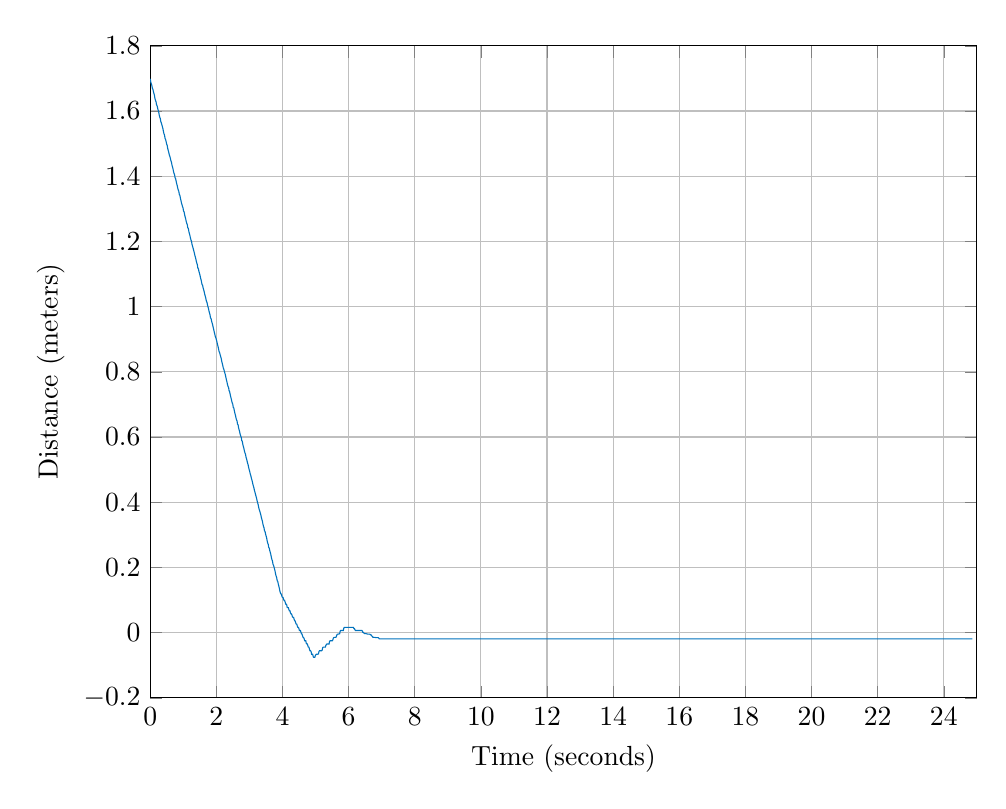
\begin{tikzpicture}

\begin{axis}[%
width=4.133in,
height=3.26in,
at={(0.693in,0.44in)},
scale only axis,
xmin=0,
xmax=25,
xmajorgrids,
xlabel={Time (seconds)},
ymin=-0.2,
ymax=1.8,
ymajorgrids,
ylabel={Distance (meters)},
axis background/.style={fill=white}
]
\addplot [color=mycolor1,solid,forget plot]
  table[row sep=crcr]{%
0	1.69871129724401\\
0.0161597069999985	1.68893572639479\\
0.0320381099999994	1.68304748664486\\
0.0480332269999981	1.67912271456059\\
0.0639209419999979	1.66931011561885\\
0.0799915179999992	1.66734738109778\\
0.095894748999998	1.65949784397757\\
0.112236309	1.65361021900933\\
0.128000544	1.64772313251249\\
0.144037290999997	1.63794410885595\\
0.160031794999998	1.63205633442079\\
0.176005682999998	1.62813189575498\\
0.192028402999997	1.61832008838933\\
0.208044257999998	1.61635749467799\\
0.223975831999999	1.60850861976092\\
0.239845890999999	1.60262157886489\\
0.255932509	1.59673502919364\\
0.272045081	1.58734001353617\\
0.288055432999998	1.58106497639806\\
0.303994013	1.57714087404251\\
0.320085219	1.56732994860591\\
0.336047623	1.56340561944332\\
0.352167114	1.55751933829978\\
0.367957239999998	1.55163277667723\\
0.384000864	1.54574694383911\\
0.400002680999998	1.53673752095665\\
0.416095590999998	1.53007361836111\\
0.432093585999999	1.52614967659862\\
0.448009974999998	1.51633972033348\\
0.464211726	1.51241574277692\\
0.480004193999998	1.5065299349548\\
0.495950020999998	1.49868218733043\\
0.512157272999998	1.49475848376015\\
0.527974259999998	1.48574768432082\\
0.543906164999999	1.4790821002072\\
0.559931816999998	1.47319656333825\\
0.576047603	1.4653494447477\\
0.592099309	1.4614252420419\\
0.607958182999998	1.45554052188685\\
0.624044353999998	1.44769340723938\\
0.640059370999999	1.44377015708712\\
0.655988042999998	1.4347569579997\\
0.674189583999999	1.42809050499233\\
0.689372704999998	1.42220547781748\\
0.704676809999999	1.41435912230833\\
0.720098040999997	1.40847385303638\\
0.736003673999999	1.40455114742055\\
0.751938995999999	1.39474336036922\\
0.768141095999997	1.39278164787541\\
0.783864349999998	1.38415554707216\\
0.799962436000001	1.37709909106128\\
0.816062182	1.37121450744656\\
0.831906223999999	1.36336883703143\\
0.848027445999999	1.35748408737176\\
0.863959540999997	1.35356162772472\\
0.879933877999999	1.34375472787583\\
0.896142252999999	1.34179332640154\\
0.911980344	1.3327763641861\\
0.927973438999999	1.32610752584645\\
0.944083456999999	1.31826243875527\\
0.961772406999998	1.31237855057905\\
0.977025619999997	1.30649432253796\\
0.992100941	1.30257231269253\\
1.008016162	1.29276624303506\\
1.024052284	1.29080502488716\\
1.040043836	1.28178351599921\\
1.056101456	1.27511612308704\\
1.072042082	1.2692326481451\\
1.088003722	1.26138833611554\\
1.104018756	1.25550464929934\\
1.120016068	1.25158296727092\\
1.136028841	1.24177772607526\\
1.152454134	1.23981668476706\\
1.168027	1.2303995072145\\
1.184022474	1.22412476633608\\
1.200019596	1.21824182103829\\
1.215844534	1.21039822757948\\
1.231866587	1.20451505767636\\
1.248032203	1.2005937590141\\
1.263980122	1.19078942043123\\
1.280011167	1.18490673794708\\
1.29606839	1.17940870504848\\
1.311915058	1.17313356596483\\
1.328096262	1.1672510988771\\
1.344009535	1.15940824885514\\
1.360016657	1.15352569176184\\
1.375985619	1.14764371378953\\
1.392028144	1.13980142041503\\
1.40798655	1.13391921114855\\
1.42402477	1.12841776192211\\
1.440059497	1.11822158188759\\
1.45603875	1.1162605804508\\
1.471952503	1.1084184254641\\
1.488035673	1.10253629143816\\
1.503981907	1.09665490151816\\
1.519956103	1.08881312554247\\
1.536030251	1.08293152143553\\
1.552009798	1.07507267952918\\
1.568032618	1.06723098008438\\
1.5838202	1.06527019760318\\
1.599864249	1.05742876912491\\
1.615959169	1.05154727112046\\
1.632048688	1.04566638010345\\
1.648019474	1.03782551190427\\
1.664054938	1.03194436384094\\
1.679953888	1.02604218763219\\
1.698397633	1.01624058473149\\
1.713703745	1.01428004472839\\
1.72889844	1.00643932715905\\
1.744129695	1.00055847314288\\
1.759945545	0.994677953425816\\
1.776049409	0.986837802029016\\
1.792043329	0.980558688723852\\
1.807978683	0.975051181247059\\
1.82404031	0.965250506013386\\
1.839987489	0.96329011844845\\
1.855994895	0.955450129911461\\
1.872343168	0.94956970168786\\
1.889012394	0.943689914530665\\
1.9044551	0.935850489903957\\
1.919998366	0.929570993774472\\
1.936042599	0.922100180707373\\
1.9551955	0.914260636445593\\
1.967938604	0.908380570722335\\
1.983951515	0.904461289654192\\
1.999907206	0.898581464602012\\
2.015889816	0.892702168501254\\
2.031923368	0.884863548697085\\
2.048048731	0.878584115504906\\
2.064144898	0.871109887908198\\
2.079977502	0.863271098039109\\
2.096045085	0.859350967097983\\
2.112068737	0.853472564200506\\
2.128073517	0.847593340588921\\
2.144261578	0.841714550055185\\
2.160036456	0.833876587396984\\
2.176083732	0.826396763295437\\
2.192723347	0.820119933701045\\
2.208038736	0.812281855159503\\
2.223876149	0.808362164955397\\
2.239849326	0.802484373461212\\
2.255899088	0.796605666066156\\
2.272052215	0.790727458630502\\
2.287967036	0.782890319311338\\
2.304064223	0.775407591406852\\
2.320043139	0.769130319900535\\
2.336038054	0.761293068547499\\
2.351829435	0.75541467613456\\
2.369982512	0.751496479134997\\
2.38512788	0.74170016002278\\
2.400280705	0.739740988787028\\
2.415837345	0.731501518293285\\
2.432007665	0.724418512415375\\
2.448062212	0.718141068284811\\
2.463904847	0.710304473858481\\
2.480109883	0.704426707604771\\
2.496265234	0.700508883353315\\
2.512023521	0.690713360854889\\
2.528088527	0.688754202437095\\
2.544039715	0.680515038507873\\
2.559966231	0.673029345138253\\
2.576072755	0.667152253082086\\
2.592026031	0.659316504360529\\
2.608029787	0.653439253292801\\
2.624161381	0.649521810331318\\
2.640087182	0.639727347084461\\
2.656085963	0.637768618929747\\
2.671960964	0.62872082387013\\
2.687938773	0.622040424101864\\
2.704019966	0.616163989895688\\
2.719945606	0.608328904385657\\
2.738228445	0.602452118238467\\
2.753453936	0.598535052312638\\
2.768958834	0.588741386154098\\
2.784172406	0.586782953034807\\
2.799987707	0.577330655479049\\
2.815978062	0.571051900275226\\
2.831936446	0.565175920436754\\
2.848171315	0.557341692739733\\
2.864070536	0.551465599918871\\
2.879906841	0.547548920191658\\
2.898319483	0.537756332694852\\
2.913432974	0.533433205478571\\
2.928504284	0.526343085141848\\
2.944032319	0.520063962159091\\
2.961627301	0.514188695073108\\
2.976743491	0.506355081664197\\
2.991888999	0.500479650243511\\
3.008038559	0.494604892109511\\
3.024039035	0.486771711290253\\
3.040029301	0.482041069001969\\
3.056029827	0.474951959878612\\
3.072002385	0.469076411879514\\
3.087935715	0.46320174307167\\
3.104126096	0.455368866665759\\
3.12008357	0.449493948992479\\
3.13626276	0.443619792502053\\
3.151976129	0.435787349831549\\
3.168037998	0.430648428519785\\
3.183919051	0.423964328230578\\
3.200040116	0.418089576280482\\
3.216189738	0.412215493214756\\
3.231910769	0.404383364085438\\
3.248055819	0.398509125431866\\
3.264056188	0.392635554648707\\
3.280027158	0.384395210111485\\
3.296231439	0.377298609904035\\
3.312036912	0.372977597796839\\
3.328016334	0.367103377074015\\
3.343968255	0.361229909607538\\
3.360014117	0.353398805192615\\
3.376034012	0.347524948726206\\
3.392055329	0.341651996907191\\
3.408026453	0.333001963896481\\
3.424020107	0.326312818280381\\
3.440119185	0.321991261436119\\
3.45601791	0.312202244186959\\
3.471905818	0.310244617298781\\
3.487985074	0.302414352466512\\
3.504023751	0.296540955638987\\
3.520007506	0.290668589105361\\
3.536027933	0.281608342510867\\
3.55201356	0.274920238752738\\
3.568069104	0.271005653666978\\
3.583991387	0.261217606003176\\
3.599856609	0.259260325908042\\
3.615886901	0.251430789588521\\
3.631882137	0.245558077424806\\
3.648018395	0.239275305161136\\
3.664186224	0.230215965222551\\
3.680057807	0.223934969536399\\
3.69610339099999	0.220020579845011\\
3.712014664	0.210234035078069\\
3.727875202	0.206319521438501\\
3.746120862	0.200447621778105\\
3.761399832	0.19457537383804\\
3.777495913	0.187469394394467\\
3.792651319	0.179231291646869\\
3.808047239	0.172950077713062\\
3.824017838	0.169036360464767\\
3.840128517	0.159250183080458\\
3.856000751	0.157293420718972\\
3.872034177	0.149465470882983\\
3.888009325	0.143181163778427\\
3.904088042	0.136485513695991\\
3.919988997	0.127837780808854\\
3.936021406	0.12196625098542\\
3.95416299399999	0.118053047831513\\
3.969390648	0.118053671948953\\
3.984691207	0.110225493363726\\
3.999839993	0.108269543967233\\
4.016042797	0.108270330969134\\
4.03203006	0.102399395843292\\
4.048061705	0.0984862594713412\\
4.06407144	0.0984872886415111\\
4.080018434	0.0941594451900318\\
4.096129343	0.0874625463582588\\
4.112024089	0.0874628361458927\\
4.127970745	0.0850950626059361\\
4.143969595	0.0768571351875145\\
4.160082283	0.0768575072346276\\
4.176027659	0.0768581011423619\\
4.192031024	0.0709877188160699\\
4.207906927	0.0670753752405857\\
4.224030191	0.0670761330116969\\
4.240131932	0.0612060493879958\\
4.256005005	0.0572940154216122\\
4.272005968	0.0572949372945433\\
4.287987546	0.0533815204179826\\
4.304032883	0.0475134286717198\\
4.320066543	0.0470990329475192\\
4.335935542	0.0466838392976991\\
4.351989792	0.0403991501322358\\
4.368078106	0.0364877379760677\\
4.384024383	0.0356612134958443\\
4.400048635	0.0297920471689561\\
4.416002176	0.0258799004666967\\
4.432025753	0.0258806330229335\\
4.448008253	0.0200118494713066\\
4.466390864	0.0160999309655905\\
4.481743225	0.0161008286024771\\
4.496877657	0.0121885054519431\\
4.512207512	0.0063207381724133\\
4.528158156	0.00632180112834302\\
4.544037839	0.00632242136469596\\
4.560025981	0.000454404614969484\\
4.576041295	-0.00387363753753234\\
4.592056829	-0.00470731206715502\\
4.608019278	-0.0105756275646269\\
4.62403573	-0.0149013097434754\\
4.640037472	-0.0153156631968081\\
4.655998012	-0.0192277355455215\\
4.672033909	-0.0250945070702824\\
4.687984735	-0.0250939779766068\\
4.704018982	-0.0250934595164349\\
4.720118501	-0.0329173827984737\\
4.736174136	-0.0348721248013601\\
4.752146888	-0.0348709099965969\\
4.768025783	-0.0407386728914312\\
4.784058266	-0.0446489610539258\\
4.800029234	-0.044647578759978\\
4.815947588	-0.0509339354580634\\
4.832000617	-0.0556813610305149\\
4.848042019	-0.0556809219308558\\
4.864082611	-0.0576362044890137\\
4.879951488	-0.0662910094797866\\
4.89594289	-0.0662904863547429\\
4.912064377	-0.0662894509891434\\
4.9304653	-0.0741117093876493\\
4.94577737	-0.0760665953911499\\
4.961679111	-0.0760653917960896\\
4.977120934	-0.0760643414184479\\
4.993380468	-0.0701963671843349\\
5.007918377	-0.0682398683273959\\
5.023956583	-0.0662835217940423\\
5.040158076	-0.0662835217940423\\
5.055902977	-0.0662824211216588\\
5.072024647	-0.0658643349305423\\
5.088030083	-0.0654448321368184\\
5.10386294	-0.0576215921086409\\
5.120073524	-0.0556658255702775\\
5.136060234	-0.055664318797668\\
5.152007599	-0.0556638147487121\\
5.168071171	-0.0556628174756462\\
5.183948769	-0.0556612890786246\\
5.200052768	-0.0537051345904236\\
5.216022674	-0.0465737605981631\\
5.232006657	-0.0446172304217491\\
5.248422187	-0.0446164371258764\\
5.263848381	-0.0446148612865487\\
5.279826202	-0.044613435982205\\
5.296176005	-0.0446126319339388\\
5.311981721	-0.0387450693181646\\
5.327945374	-0.0367888634441205\\
5.344000982	-0.0348331431779674\\
5.359946961	-0.0348324128066471\\
5.376003225	-0.0348310055285577\\
5.392103125	-0.0348303500075755\\
5.4080127	-0.0348288571865003\\
5.424028947	-0.0270078227380737\\
5.440033359	-0.0250517945274167\\
5.456060079	-0.0250504279724031\\
5.47202798	-0.025049739378282\\
5.487982025	-0.0250485216894465\\
5.504321258	-0.0250478224621185\\
5.520074267	-0.0230912347651395\\
5.536756396	-0.0172256489887266\\
5.552058505	-0.0152703289659444\\
5.568074951	-0.0148481242482632\\
5.584150324	-0.0144250438543301\\
5.600060666	-0.0144243973948623\\
5.616020499	-0.0144231150495533\\
5.632025239	-0.0105112662723323\\
5.648037045	-0.00660175890715542\\
5.664116752	-0.00464606729543604\\
5.679942383	-0.00464437671218132\\
5.698385246	-0.00464437671218132\\
5.713696811	-0.00336876985330625\\
5.728932413	-0.00336783530132267\\
5.744098644	0.0044522415300019\\
5.760014211	0.0064083608881389\\
5.775945737	0.00640923172839569\\
5.79213369	0.00641081678433286\\
5.808040699	0.00641169806611774\\
5.823987022	0.00641345018815964\\
5.840063859	0.00641505612753535\\
5.85608706	0.0142336466099027\\
5.872151891	0.0161895107638446\\
5.88801638	0.0161909898158903\\
5.904064434	0.0161918175892559\\
5.919998809	0.0161934627540379\\
5.93607576	0.0161949625703395\\
5.954263675	0.0161958007256291\\
5.968022303	0.0161974666542841\\
5.983883145	0.0161989872347965\\
6.000049104	0.0161998357719848\\
6.015938219	0.0162006739272744\\
6.032082775	0.0162030638091391\\
6.04805246	0.0162030638091391\\
6.064082037	0.0162047712653877\\
6.080065318	0.0162056301844482\\
6.096283305	0.016207192293243\\
6.112111165	0.0162089205132103\\
6.12803681	0.0162097898141171\\
6.144032264	0.0162113726869815\\
6.15999543899999	0.0123042193904623\\
6.176025307	0.0123060430035689\\
6.192050662	0.00839983725200977\\
6.207921611	0.00644715815732333\\
6.22418061	0.00644907734205402\\
6.239899469	0.00645085034712545\\
6.255993164	0.00645182560141855\\
6.271981044	0.00645376566872891\\
6.288022904	0.0064555595567759\\
6.304075306	0.00645654525231443\\
6.320040812	0.00645850620214539\\
6.336001828	0.00646032097311311\\
6.35187561	0.00646131710986664\\
6.368084163	0.00646230280540494\\
6.383953458	0.00646329894215891\\
6.400024741	0.00646513459599229\\
6.416083481	0.00451326951456554\\
6.432049987	0.000606989229278154\\
6.448068159	0.000608994846316602\\
6.464017704	-0.00134318265871802\\
6.480020071	-0.00329427859929332\\
6.496229008	-0.00329225198046768\\
6.511858828	-0.00329114941473319\\
6.530239581	-0.00328895478388502\\
6.5453811	-0.00371740052756842\\
6.560536606	-0.00414678081236741\\
6.575981488	-0.00457574031183228\\
6.592027873	-0.00457367168961809\\
6.608653865	-0.00457288898670516\\
6.624052054	-0.00457133409455657\\
6.640030645	-0.00456924447074214\\
6.656037202	-0.00652194560537556\\
6.671994857	-0.00652116290246241\\
6.687993142	-0.00847393884510206\\
6.704031864	-0.0104246475733203\\
6.720040167	-0.0123757937441658\\
6.735860388	-0.0143278084155758\\
6.752142985	-0.0143255269942206\\
6.767895372	-0.0147532289280985\\
6.783825069	-0.0147523392813249\\
6.799921703	-0.0147503776559519\\
6.815882875	-0.0151789480904481\\
6.832018811	-0.0151771582238365\\
6.848020074	-0.0151755163814231\\
6.864051549	-0.0151746055885482\\
6.880044717	-0.0151727945758353\\
6.896191653	-0.0151711315869532\\
6.912056843	-0.0171233296396782\\
6.92827234	-0.0190746920050473\\
6.944046239	-0.0190746920050473\\
6.961524159	-0.0190746920050473\\
6.977450972	-0.0190746920050473\\
6.992599246	-0.0190746920050473\\
7.008127417	-0.0190746920050473\\
7.023842395	-0.0190746920050473\\
7.040040934	-0.0190746920050473\\
7.056096008	-0.0190746920050473\\
7.072035099	-0.0190746920050473\\
7.088049521	-0.0190746920050473\\
7.104026435	-0.0190746920050473\\
7.120011623	-0.0190746920050473\\
7.136038122	-0.0190746920050473\\
7.152012828	-0.0190746920050473\\
7.167907396	-0.0190746920050473\\
7.184216646	-0.0190746920050473\\
7.200091968	-0.0190746920050473\\
7.215989592	-0.0190746920050473\\
7.231833071	-0.0190746920050473\\
7.248330282	-0.0190746920050473\\
7.26403765	-0.0190746920050473\\
7.279981706	-0.0190746920050473\\
7.296229812	-0.0190746920050473\\
7.312106607	-0.0190746920050473\\
7.328115852	-0.0190746920050473\\
7.347357186	-0.0190746920050473\\
7.360618501	-0.0190746920050473\\
7.375853683	-0.0190746920050473\\
7.392082657	-0.0190746920050473\\
7.408037023	-0.0190746920050473\\
7.424167001	-0.0190746920050473\\
7.440051263	-0.0190746920050473\\
7.455951863	-0.0190746920050473\\
7.471980511	-0.0190746920050473\\
7.488062711	-0.0190746920050473\\
7.50406574399999	-0.0190746920050473\\
7.520029658	-0.0190746920050473\\
7.536123601	-0.0190746920050473\\
7.551947701	-0.0190746920050473\\
7.568152163	-0.0190746920050473\\
7.584046088	-0.0190746920050473\\
7.59997950499999	-0.0190746920050473\\
7.615931435	-0.0190746920050473\\
7.63193073299999	-0.0190746920050473\\
7.647994752	-0.0190746920050473\\
7.664175922	-0.0190746920050473\\
7.679965259	-0.0190746920050473\\
7.695999804	-0.0190746920050473\\
7.712042392	-0.0190746920050473\\
7.728070754	-0.0190746920050473\\
7.74400096	-0.0190746920050473\\
7.760090146	-0.0190746920050473\\
7.775972463	-0.0190746920050473\\
7.79210594	-0.0190746920050473\\
7.807910945	-0.0190746920050473\\
7.826481575	-0.0190746920050473\\
7.840035591	-0.0190746920050473\\
7.855958237	-0.0190746920050473\\
7.872038788	-0.0190746920050473\\
7.887981322	-0.0190746920050473\\
7.90405819	-0.0190746920050473\\
7.920025129	-0.0190746920050473\\
7.936070311	-0.0190746920050473\\
7.95442091	-0.0190746920050473\\
7.970032808	-0.0190746920050473\\
7.985465228	-0.0190746920050473\\
8.000631693	-0.0190746920050473\\
8.015877657	-0.0190746920050473\\
8.031841158	-0.0190746920050473\\
8.048041935	-0.0190746920050473\\
8.064091872	-0.0190746920050473\\
8.080200063	-0.0190746920050473\\
8.096275027	-0.0190746920050473\\
8.112130566	-0.0190746920050473\\
8.128056864	-0.0190746920050473\\
8.143986503	-0.0190746920050473\\
8.16003903099999	-0.0190746920050473\\
8.176019812	-0.0190746920050473\\
8.192062197	-0.0190746920050473\\
8.207986459	-0.0190746920050473\\
8.223936542	-0.0190746920050473\\
8.240084434	-0.0190746920050473\\
8.25601462	-0.0190746920050473\\
8.27198565599999	-0.0190746920050473\\
8.288014618	-0.0190746920050473\\
8.304042044	-0.0190746920050473\\
8.320048804	-0.0190746920050473\\
8.336020914	-0.0190746920050473\\
8.352109304	-0.0190746920050473\\
8.368036166	-0.0190746920050473\\
8.384032565	-0.0190746920050473\\
8.400153247	-0.0190746920050473\\
8.416017998	-0.0190746920050473\\
8.432060103	-0.0190746920050473\\
8.448029026	-0.0190746920050473\\
8.464155182	-0.0190746920050473\\
8.479910554	-0.0190746920050473\\
8.496110741	-0.0190746920050473\\
8.512041377	-0.0190746920050473\\
8.528053603	-0.0190746920050473\\
8.5440378	-0.0190746920050473\\
8.560008308	-0.0190746920050473\\
8.576030592	-0.0190746920050473\\
8.592044783	-0.0190746920050473\\
8.608031017	-0.0190746920050473\\
8.62401557499999	-0.0190746920050473\\
8.640046203	-0.0190746920050473\\
8.656053173	-0.0190746920050473\\
8.672049955	-0.0190746920050473\\
8.688048636	-0.0190746920050473\\
8.704018567	-0.0190746920050473\\
8.720117199	-0.0190746920050473\\
8.735884545	-0.0190746920050473\\
8.752065129	-0.0190746920050473\\
8.768022497	-0.0190746920050473\\
8.783983003	-0.0190746920050473\\
8.800052132	-0.0190746920050473\\
8.81598551999999	-0.0190746920050473\\
8.832077187	-0.0190746920050473\\
8.848160304	-0.0190746920050473\\
8.864148186	-0.0190746920050473\\
8.880060631	-0.0190746920050473\\
8.896150063	-0.0190746920050473\\
8.91204172199999	-0.0190746920050473\\
8.928087221	-0.0190746920050473\\
8.943992198	-0.0190746920050473\\
8.962038489	-0.0190746920050473\\
8.97723275499999	-0.0190746920050473\\
8.992413163	-0.0190746920050473\\
9.008046767	-0.0190746920050473\\
9.024117446	-0.0190746920050473\\
9.040125834	-0.0190746920050473\\
9.05604500499999	-0.0190746920050473\\
9.072428207	-0.0190746920050473\\
9.088008385	-0.0190746920050473\\
9.104071111	-0.0190746920050473\\
9.119975429	-0.0190746920050473\\
9.135911819	-0.0190746920050473\\
9.152010125	-0.0190746920050473\\
9.168027158	-0.0190746920050473\\
9.183971459	-0.0190746920050473\\
9.200329666	-0.0190746920050473\\
9.216105473	-0.0190746920050473\\
9.231951862	-0.0190746920050473\\
9.247956231	-0.0190746920050473\\
9.263936089	-0.0190746920050473\\
9.27997825499999	-0.0190746920050473\\
9.296043407	-0.0190746920050473\\
9.31200781	-0.0190746920050473\\
9.328068476	-0.0190746920050473\\
9.343996109	-0.0190746920050473\\
9.360029443	-0.0190746920050473\\
9.376059964	-0.0190746920050473\\
9.392060099	-0.0190746920050473\\
9.408022713	-0.0190746920050473\\
9.424026481	-0.0190746920050473\\
9.439842754	-0.0190746920050473\\
9.45612246099999	-0.0190746920050473\\
9.47194129	-0.0190746920050473\\
9.487846234	-0.0190746920050473\\
9.503996775	-0.0190746920050473\\
9.520063444	-0.0190746920050473\\
9.53605973	-0.0190746920050473\\
9.551842657	-0.0190746920050473\\
9.567985474	-0.0190746920050473\\
9.583973095	-0.0190746920050473\\
9.600094845	-0.0190746920050473\\
9.615999506	-0.0190746920050473\\
9.63206045	-0.0190746920050473\\
9.647986517	-0.0190746920050473\\
9.66403696	-0.0190746920050473\\
9.6800219	-0.0190746920050473\\
9.69633846499999	-0.0190746920050473\\
9.71200180299999	-0.0190746920050473\\
9.727943566	-0.0190746920050473\\
9.743880255	-0.0190746920050473\\
9.760009592	-0.0190746920050473\\
9.77591782	-0.0190746920050473\\
9.792128023	-0.0190746920050473\\
9.807998384	-0.0190746920050473\\
9.824041778	-0.0190746920050473\\
9.839929408	-0.0190746920050473\\
9.856133159	-0.0190746920050473\\
9.87203671	-0.0190746920050473\\
9.887991558	-0.0190746920050473\\
9.904069088	-0.0190746920050473\\
9.91998593899999	-0.0190746920050473\\
9.936009968	-0.0190746920050473\\
9.954419339	-0.0190746920050473\\
9.969493511	-0.0190746920050473\\
9.984564415	-0.0190746920050473\\
9.999949428	-0.0190746920050473\\
10.01603085	-0.0190746920050473\\
10.031982539	-0.0190746920050473\\
10.047971055	-0.0190746920050473\\
10.064137549	-0.0190746920050473\\
10.080024832	-0.0190746920050473\\
10.096311882	-0.0190746920050473\\
10.111981522	-0.0190746920050473\\
10.128014125	-0.0190746920050473\\
10.143918003	-0.0190746920050473\\
10.160075898	-0.0190746920050473\\
10.176041825	-0.0190746920050473\\
10.191946311	-0.0190746920050473\\
10.207993503	-0.0190746920050473\\
10.223840547	-0.0190746920050473\\
10.242181889	-0.0190746920050473\\
10.257547214	-0.0190746920050473\\
10.272842035	-0.0190746920050473\\
10.288258415	-0.0190746920050473\\
10.30402324	-0.0190746920050473\\
10.319987257	-0.0190746920050473\\
10.336007504	-0.0190746920050473\\
10.351845281	-0.0190746920050473\\
10.367901405	-0.0190746920050473\\
10.383952171	-0.0190746920050473\\
10.400084774	-0.0190746920050473\\
10.416048786	-0.0190746920050473\\
10.432052679	-0.0190746920050473\\
10.447944806	-0.0190746920050473\\
10.464018899	-0.0190746920050473\\
10.479930656	-0.0190746920050473\\
10.496009384	-0.0190746920050473\\
10.512003509	-0.0190746920050473\\
10.528001341	-0.0190746920050473\\
10.543906675	-0.0190746920050473\\
10.560054811	-0.0190746920050473\\
10.575963898	-0.0190746920050473\\
10.592071361	-0.0190746920050473\\
10.608016686	-0.0190746920050473\\
10.624253612	-0.0190746920050473\\
10.639974423	-0.0190746920050473\\
10.656005623	-0.0190746920050473\\
10.6720202	-0.0190746920050473\\
10.688051613	-0.0190746920050473\\
10.704094484	-0.0190746920050473\\
10.719905633	-0.0190746920050473\\
10.736099586	-0.0190746920050473\\
10.752060592	-0.0190746920050473\\
10.767958262	-0.0190746920050473\\
10.78385751	-0.0190746920050473\\
10.800008416	-0.0190746920050473\\
10.815938755	-0.0190746920050473\\
10.832015205	-0.0190746920050473\\
10.84798706	-0.0190746920050473\\
10.863915459	-0.0190746920050473\\
10.879975807	-0.0190746920050473\\
10.896156141	-0.0190746920050473\\
10.912156856	-0.0190746920050473\\
10.928125038	-0.0190746920050473\\
10.94389824	-0.0190746920050473\\
10.961753412	-0.0190746920050473\\
10.976892011	-0.0190746920050473\\
10.991989265	-0.0190746920050473\\
11.007936167	-0.0190746920050473\\
11.023980819	-0.0190746920050473\\
11.039995061	-0.0190746920050473\\
11.055939814	-0.0190746920050473\\
11.072026706	-0.0190746920050473\\
11.087993069	-0.0190746920050473\\
11.104061448	-0.0190746920050473\\
11.119990536	-0.0190746920050473\\
11.13604776	-0.0190746920050473\\
11.151991937	-0.0190746920050473\\
11.167951617	-0.0190746920050473\\
11.184098376	-0.0190746920050473\\
11.200034054	-0.0190746920050473\\
11.216048521	-0.0190746920050473\\
11.232185	-0.0190746920050473\\
11.247942829	-0.0190746920050473\\
11.264146716	-0.0190746920050473\\
11.279973192	-0.0190746920050473\\
11.296176855	-0.0190746920050473\\
11.312011646	-0.0190746920050473\\
11.32802642	-0.0190746920050473\\
11.344102481	-0.0190746920050473\\
11.360021482	-0.0190746920050473\\
11.375974636	-0.0190746920050473\\
11.392056679	-0.0190746920050473\\
11.408017455	-0.0190746920050473\\
11.424039889	-0.0190746920050473\\
11.440068771	-0.0190746920050473\\
11.455963834	-0.0190746920050473\\
11.472028245	-0.0190746920050473\\
11.487850341	-0.0190746920050473\\
11.503963567	-0.0190746920050473\\
11.519898403	-0.0190746920050473\\
11.536050687	-0.0190746920050473\\
11.55205493	-0.0190746920050473\\
11.568074338	-0.0190746920050473\\
11.583873613	-0.0190746920050473\\
11.600053498	-0.0190746920050473\\
11.615978068	-0.0190746920050473\\
11.632026927	-0.0190746920050473\\
11.647987738	-0.0190746920050473\\
11.664023823	-0.0190746920050473\\
11.679976365	-0.0190746920050473\\
11.696077372	-0.0190746920050473\\
11.71197076	-0.0190746920050473\\
11.727841005	-0.0190746920050473\\
11.744121961	-0.0190746920050473\\
11.760058751	-0.0190746920050473\\
11.775981456	-0.0190746920050473\\
11.792139803	-0.0190746920050473\\
11.808040402	-0.0190746920050473\\
11.824030439	-0.0190746920050473\\
11.839930198	-0.0190746920050473\\
11.856071871	-0.0190746920050473\\
11.872051192	-0.0190746920050473\\
11.887960344	-0.0190746920050473\\
11.904064275	-0.0190746920050473\\
11.920007937	-0.0190746920050473\\
11.936042439	-0.0190746920050473\\
11.954345124	-0.0190746920050473\\
11.969600887	-0.0190746920050473\\
11.984774743	-0.0190746920050473\\
12.000021787	-0.0190746920050473\\
12.015990606	-0.0190746920050473\\
12.032030576	-0.0190746920050473\\
12.048008515	-0.0190746920050473\\
12.064101971	-0.0190746920050473\\
12.079999859	-0.0190746920050473\\
12.096173406	-0.0190746920050473\\
12.111978598	-0.0190746920050473\\
12.128102533	-0.0190746920050473\\
12.143986169	-0.0190746920050473\\
12.159931471	-0.0190746920050473\\
12.175995508	-0.0190746920050473\\
12.192126894	-0.0190746920050473\\
12.207915106	-0.0190746920050473\\
12.223849699	-0.0190746920050473\\
12.240104586	-0.0190746920050473\\
12.255989618	-0.0190746920050473\\
12.272108488	-0.0190746920050473\\
12.288026742	-0.0190746920050473\\
12.304032474	-0.0190746920050473\\
12.319919155	-0.0190746920050473\\
12.336026423	-0.0190746920050473\\
12.351984568	-0.0190746920050473\\
12.36799499	-0.0190746920050473\\
12.383991041	-0.0190746920050473\\
12.40011831	-0.0190746920050473\\
12.415925558	-0.0190746920050473\\
12.432058415	-0.0190746920050473\\
12.44804794	-0.0190746920050473\\
12.464110415	-0.0190746920050473\\
12.479914115	-0.0190746920050473\\
12.495969561	-0.0190746920050473\\
12.512145343	-0.0190746920050473\\
12.528196013	-0.0190746920050473\\
12.543936511	-0.0190746920050473\\
12.559966416	-0.0190746920050473\\
12.575993634	-0.0190746920050473\\
12.592045531	-0.0190746920050473\\
12.607943409	-0.0190746920050473\\
12.624102934	-0.0190746920050473\\
12.640012173	-0.0190746920050473\\
12.65615738	-0.0190746920050473\\
12.672005105	-0.0190746920050473\\
12.687947837	-0.0190746920050473\\
12.703857148	-0.0190746920050473\\
12.719957478	-0.0190746920050473\\
12.735929695	-0.0190746920050473\\
12.751939591	-0.0190746920050473\\
12.76804339	-0.0190746920050473\\
12.783981093	-0.0190746920050473\\
12.800015786	-0.0190746920050473\\
12.815985707	-0.0190746920050473\\
12.832077238	-0.0190746920050473\\
12.847975226	-0.0190746920050473\\
12.863951035	-0.0190746920050473\\
12.879817968	-0.0190746920050473\\
12.898329922	-0.0190746920050473\\
12.913635623	-0.0190746920050473\\
12.928822896	-0.0190746920050473\\
12.944141417	-0.0190746920050473\\
12.961861101	-0.0190746920050473\\
12.977067905	-0.0190746920050473\\
12.992354105	-0.0190746920050473\\
13.007968762	-0.0190746920050473\\
13.024084042	-0.0190746920050473\\
13.041294187	-0.0190746920050473\\
13.056377386	-0.0190746920050473\\
13.071859735	-0.0190746920050473\\
13.088020699	-0.0190746920050473\\
13.104060779	-0.0190746920050473\\
13.120021364	-0.0190746920050473\\
13.136209198	-0.0190746920050473\\
13.15198511	-0.0190746920050473\\
13.167973415	-0.0190746920050473\\
13.183933769	-0.0190746920050473\\
13.199982266	-0.0190746920050473\\
13.216107117	-0.0190746920050473\\
13.231896675	-0.0190746920050473\\
13.247975103	-0.0190746920050473\\
13.265740064	-0.0190746920050473\\
13.280772699	-0.0190746920050473\\
13.296028956	-0.0190746920050473\\
13.311972453	-0.0190746920050473\\
13.32817736	-0.0190746920050473\\
13.344024287	-0.0190746920050473\\
13.360055672	-0.0190746920050473\\
13.375948308	-0.0190746920050473\\
13.392040151	-0.0190746920050473\\
13.407889418	-0.0190746920050473\\
13.424004142	-0.0190746920050473\\
13.440038052	-0.0190746920050473\\
13.4560137	-0.0190746920050473\\
13.472000736	-0.0190746920050473\\
13.490213617	-0.0190746920050473\\
13.505429094	-0.0190746920050473\\
13.52066168	-0.0190746920050473\\
13.536031341	-0.0190746920050473\\
13.552165255	-0.0190746920050473\\
13.568039037	-0.0190746920050473\\
13.583982463	-0.0190746920050473\\
13.600090446	-0.0190746920050473\\
13.616007713	-0.0190746920050473\\
13.632086251	-0.0190746920050473\\
13.648004273	-0.0190746920050473\\
13.663916969	-0.0190746920050473\\
13.679885169	-0.0190746920050473\\
13.69607269	-0.0190746920050473\\
13.711928864	-0.0190746920050473\\
13.727840392	-0.0190746920050473\\
13.746186255	-0.0190746920050473\\
13.761514983	-0.0190746920050473\\
13.776717546	-0.0190746920050473\\
13.792096959	-0.0190746920050473\\
13.808066698	-0.0190746920050473\\
13.824055471	-0.0190746920050473\\
13.840026692	-0.0190746920050473\\
13.85609019	-0.0190746920050473\\
13.872063824	-0.0190746920050473\\
13.88799977	-0.0190746920050473\\
13.90403201	-0.0190746920050473\\
13.919998037	-0.0190746920050473\\
13.935995265	-0.0190746920050473\\
13.95437071	-0.0190746920050473\\
13.969473101	-0.0190746920050473\\
13.984630877	-0.0190746920050473\\
14.000035212	-0.0190746920050473\\
14.016035313	-0.0190746920050473\\
14.031898991	-0.0190746920050473\\
14.047852831	-0.0190746920050473\\
14.064161409	-0.0190746920050473\\
14.079916593	-0.0190746920050473\\
14.096102855	-0.0190746920050473\\
14.111976958	-0.0190746920050473\\
14.12797426	-0.0190746920050473\\
14.144012668	-0.0190746920050473\\
14.160044558	-0.0190746920050473\\
14.175961709	-0.0190746920050473\\
14.192042305	-0.0190746920050473\\
14.208049652	-0.0190746920050473\\
14.224001116	-0.0190746920050473\\
14.240155139	-0.0190746920050473\\
14.256090979	-0.0190746920050473\\
14.272063903	-0.0190746920050473\\
14.28797831	-0.0190746920050473\\
14.303983426	-0.0190746920050473\\
14.320013633	-0.0190746920050473\\
14.336042573	-0.0190746920050473\\
14.351997199	-0.0190746920050473\\
14.36802878	-0.0190746920050473\\
14.383966503	-0.0190746920050473\\
14.400057874	-0.0190746920050473\\
14.415985273	-0.0190746920050473\\
14.432045383	-0.0190746920050473\\
14.448058382	-0.0190746920050473\\
14.46406445	-0.0190746920050473\\
14.479910137	-0.0190746920050473\\
14.49607347	-0.0190746920050473\\
14.512028174	-0.0190746920050473\\
14.527908512	-0.0190746920050473\\
14.543920158	-0.0190746920050473\\
14.560094903	-0.0190746920050473\\
14.575994334	-0.0190746920050473\\
14.592083014	-0.0190746920050473\\
14.608016698	-0.0190746920050473\\
14.623979878	-0.0190746920050473\\
14.640039582	-0.0190746920050473\\
14.658631804	-0.0190746920050473\\
14.673926435	-0.0190746920050473\\
14.689106326	-0.0190746920050473\\
14.704237437	-0.0190746920050473\\
14.720017432	-0.0190746920050473\\
14.736000604	-0.0190746920050473\\
14.751897312	-0.0190746920050473\\
14.76799095	-0.0190746920050473\\
14.783951428	-0.0190746920050473\\
14.799989254	-0.0190746920050473\\
14.816017647	-0.0190746920050473\\
14.83207217	-0.0190746920050473\\
14.847917306	-0.0190746920050473\\
14.864260418	-0.0190746920050473\\
14.880000474	-0.0190746920050473\\
14.896367052	-0.0190746920050473\\
14.911982171	-0.0190746920050473\\
14.928100222	-0.0190746920050473\\
14.943937995	-0.0190746920050473\\
14.961505084	-0.0190746920050473\\
14.976719449	-0.0190746920050473\\
14.992708124	-0.0190746920050473\\
15.008074242	-0.0190746920050473\\
15.024059109	-0.0190746920050473\\
15.040035048	-0.0190746920050473\\
15.055998653	-0.0190746920050473\\
15.072032675	-0.0190746920050473\\
15.088002988	-0.0190746920050473\\
15.104054268	-0.0190746920050473\\
15.12001629	-0.0190746920050473\\
15.136030935	-0.0190746920050473\\
15.151992881	-0.0190746920050473\\
15.16803866	-0.0190746920050473\\
15.183995224	-0.0190746920050473\\
15.200043959	-0.0190746920050473\\
15.216020123	-0.0190746920050473\\
15.232088154	-0.0190746920050473\\
15.247962883	-0.0190746920050473\\
15.264254574	-0.0190746920050473\\
15.279998857	-0.0190746920050473\\
15.296281451	-0.0190746920050473\\
15.312007224	-0.0190746920050473\\
15.328021525	-0.0190746920050473\\
15.343924693	-0.0190746920050473\\
15.360020235	-0.0190746920050473\\
15.375979707	-0.0190746920050473\\
15.392074807	-0.0190746920050473\\
15.4080369	-0.0190746920050473\\
15.423993571	-0.0190746920050473\\
15.440044119	-0.0190746920050473\\
15.456149216	-0.0190746920050473\\
15.471981967	-0.0190746920050473\\
15.487863715	-0.0190746920050473\\
15.503998821	-0.0190746920050473\\
15.519946955	-0.0190746920050473\\
15.535932565	-0.0190746920050473\\
15.552059282	-0.0190746920050473\\
15.567950071	-0.0190746920050473\\
15.583928838	-0.0190746920050473\\
15.600016627	-0.0190746920050473\\
15.615932929	-0.0190746920050473\\
15.632057563	-0.0190746920050473\\
15.647974133	-0.0190746920050473\\
15.664152802	-0.0190746920050473\\
15.679981683	-0.0190746920050473\\
15.696198852	-0.0190746920050473\\
15.712040264	-0.0190746920050473\\
15.727842035	-0.0190746920050473\\
15.744097697	-0.0190746920050473\\
15.759945528	-0.0190746920050473\\
15.775844782	-0.0190746920050473\\
15.791876812	-0.0190746920050473\\
15.807852088	-0.0190746920050473\\
15.823862428	-0.0190746920050473\\
15.840023283	-0.0190746920050473\\
15.855884566	-0.0190746920050473\\
15.871958613	-0.0190746920050473\\
15.88802791	-0.0190746920050473\\
15.90401053	-0.0190746920050473\\
15.920018427	-0.0190746920050473\\
15.936069236	-0.0190746920050473\\
15.954402605	-0.0190746920050473\\
15.969881294	-0.0190746920050473\\
15.984989983	-0.0190746920050473\\
16.00027288	-0.0190746920050473\\
16.01600951	-0.0190746920050473\\
16.031859208	-0.0190746920050473\\
16.04780463	-0.0190746920050473\\
16.064065329	-0.0190746920050473\\
16.080016262	-0.0190746920050473\\
16.096154164	-0.0190746920050473\\
16.112023546	-0.0190746920050473\\
16.128038214	-0.0190746920050473\\
16.144233139	-0.0190746920050473\\
16.160047443	-0.0190746920050473\\
16.176083208	-0.0190746920050473\\
16.191986453	-0.0190746920050473\\
16.208033744	-0.0190746920050473\\
16.223970191	-0.0190746920050473\\
16.2398523	-0.0190746920050473\\
16.255910614	-0.0190746920050473\\
16.271863341	-0.0190746920050473\\
16.287877425	-0.0190746920050473\\
16.304023761	-0.0190746920050473\\
16.320012218	-0.0190746920050473\\
16.336074036	-0.0190746920050473\\
16.352134027	-0.0190746920050473\\
16.368204205	-0.0190746920050473\\
16.383995768	-0.0190746920050473\\
16.400038268	-0.0190746920050473\\
16.416009	-0.0190746920050473\\
16.431842075	-0.0190746920050473\\
16.448002864	-0.0190746920050473\\
16.464033426	-0.0190746920050473\\
16.480022769	-0.0190746920050473\\
16.496115231	-0.0190746920050473\\
16.512289109	-0.0190746920050473\\
16.528011935	-0.0190746920050473\\
16.543892275	-0.0190746920050473\\
16.56212276	-0.0190746920050473\\
16.57722955	-0.0190746920050473\\
16.592295954	-0.0190746920050473\\
16.607984222	-0.0190746920050473\\
16.62410717	-0.0190746920050473\\
16.639881247	-0.0190746920050473\\
16.658282741	-0.0190746920050473\\
16.673478132	-0.0190746920050473\\
16.688653213	-0.0190746920050473\\
16.704194162	-0.0190746920050473\\
16.720033512	-0.0190746920050473\\
16.736019635	-0.0190746920050473\\
16.752009501	-0.0190746920050473\\
16.767990572	-0.0190746920050473\\
16.784105401	-0.0190746920050473\\
16.800015231	-0.0190746920050473\\
16.816002061	-0.0190746920050473\\
16.832008619	-0.0190746920050473\\
16.847897314	-0.0190746920050473\\
16.863925596	-0.0190746920050473\\
16.880137952	-0.0190746920050473\\
16.895960994	-0.0190746920050473\\
16.914281783	-0.0190746920050473\\
16.929934661	-0.0190746920050473\\
16.945342984	-0.0190746920050473\\
16.960263709	-0.0190746920050473\\
16.975831538	-0.0190746920050473\\
16.99192098	-0.0190746920050473\\
17.007997753	-0.0190746920050473\\
17.024033474	-0.0190746920050473\\
17.039957638	-0.0190746920050473\\
17.056297991	-0.0190746920050473\\
17.072005116	-0.0190746920050473\\
17.088032337	-0.0190746920050473\\
17.103927044	-0.0190746920050473\\
17.11988812	-0.0190746920050473\\
17.136010334	-0.0190746920050473\\
17.152036342	-0.0190746920050473\\
17.168014692	-0.0190746920050473\\
17.184013078	-0.0190746920050473\\
17.199981288	-0.0190746920050473\\
17.215890801	-0.0190746920050473\\
17.231891825	-0.0190746920050473\\
17.248071937	-0.0190746920050473\\
17.264020134	-0.0190746920050473\\
17.280137368	-0.0190746920050473\\
17.295996117	-0.0190746920050473\\
17.312017424	-0.0190746920050473\\
17.328017744	-0.0190746920050473\\
17.344110368	-0.0190746920050473\\
17.360058365	-0.0190746920050473\\
17.376052275	-0.0190746920050473\\
17.392011561	-0.0190746920050473\\
17.408133216	-0.0190746920050473\\
17.424149582	-0.0190746920050473\\
17.440131154	-0.0190746920050473\\
17.456107625	-0.0190746920050473\\
17.472061494	-0.0190746920050473\\
17.488024953	-0.0190746920050473\\
17.504025396	-0.0190746920050473\\
17.519881624	-0.0190746920050473\\
17.535953396	-0.0190746920050473\\
17.552073427	-0.0190746920050473\\
17.568327787	-0.0190746920050473\\
17.584063126	-0.0190746920050473\\
17.600006793	-0.0190746920050473\\
17.616020482	-0.0190746920050473\\
17.63202191	-0.0190746920050473\\
17.648035049	-0.0190746920050473\\
17.664060666	-0.0190746920050473\\
17.680126274	-0.0190746920050473\\
17.696125887	-0.0190746920050473\\
17.712318614	-0.0190746920050473\\
17.727854137	-0.0190746920050473\\
17.744073049	-0.0190746920050473\\
17.759969957	-0.0190746920050473\\
17.775929065	-0.0190746920050473\\
17.792023494	-0.0190746920050473\\
17.808058412	-0.0190746920050473\\
17.823998105	-0.0190746920050473\\
17.840019477	-0.0190746920050473\\
17.855978844	-0.0190746920050473\\
17.872005428	-0.0190746920050473\\
17.888040291	-0.0190746920050473\\
17.903961697	-0.0190746920050473\\
17.920024659	-0.0190746920050473\\
17.935977917	-0.0190746920050473\\
17.954456165	-0.0190746920050473\\
17.969672849	-0.0190746920050473\\
17.984994447	-0.0190746920050473\\
18.000271955	-0.0190746920050473\\
18.01588217	-0.0190746920050473\\
18.03252904	-0.0190746920050473\\
18.047841275	-0.0190746920050473\\
18.06608627	-0.0190746920050473\\
18.081291205	-0.0190746920050473\\
18.096521953	-0.0190746920050473\\
18.112388562	-0.0190746920050473\\
18.128018843	-0.0190746920050473\\
18.144415454	-0.0190746920050473\\
18.160026689	-0.0190746920050473\\
18.176049735	-0.0190746920050473\\
18.192070411	-0.0190746920050473\\
18.20804606	-0.0190746920050473\\
18.224038855	-0.0190746920050473\\
18.240063683	-0.0190746920050473\\
18.256144635	-0.0190746920050473\\
18.27226639	-0.0190746920050473\\
18.288050645	-0.0190746920050473\\
18.303963732	-0.0190746920050473\\
18.320025201	-0.0190746920050473\\
18.335968827	-0.0190746920050473\\
18.352107596	-0.0190746920050473\\
18.367862927	-0.0190746920050473\\
18.384014507	-0.0190746920050473\\
18.399921297	-0.0190746920050473\\
18.416041306	-0.0190746920050473\\
18.432124318	-0.0190746920050473\\
18.447870167	-0.0190746920050473\\
18.464028499	-0.0190746920050473\\
18.480020249	-0.0190746920050473\\
18.495858551	-0.0190746920050473\\
18.511843853	-0.0190746920050473\\
18.528047098	-0.0190746920050473\\
18.544071838	-0.0190746920050473\\
18.560014226	-0.0190746920050473\\
18.575946589	-0.0190746920050473\\
18.592165421	-0.0190746920050473\\
18.607910067	-0.0190746920050473\\
18.624064717	-0.0190746920050473\\
18.6399619	-0.0190746920050473\\
18.655970331	-0.0190746920050473\\
18.671966441	-0.0190746920050473\\
18.688036088	-0.0190746920050473\\
18.704078703	-0.0190746920050473\\
18.719964218	-0.0190746920050473\\
18.735874777	-0.0190746920050473\\
18.752004307	-0.0190746920050473\\
18.768027288	-0.0190746920050473\\
18.784034439	-0.0190746920050473\\
18.800072173	-0.0190746920050473\\
18.816012041	-0.0190746920050473\\
18.832036156	-0.0190746920050473\\
18.848070671	-0.0190746920050473\\
18.864051913	-0.0190746920050473\\
18.880203621	-0.0190746920050473\\
18.896030688	-0.0190746920050473\\
18.912248025	-0.0190746920050473\\
18.928023364	-0.0190746920050473\\
18.944022832	-0.0190746920050473\\
18.961783239	-0.0190746920050473\\
18.977057965	-0.0190746920050473\\
18.992663766	-0.0190746920050473\\
19.008089765	-0.0190746920050473\\
19.02401516	-0.0190746920050473\\
19.040134995	-0.0190746920050473\\
19.05606468	-0.0190746920050473\\
19.071920094	-0.0190746920050473\\
19.087969226	-0.0190746920050473\\
19.103930242	-0.0190746920050473\\
19.120103079	-0.0190746920050473\\
19.136025166	-0.0190746920050473\\
19.152090202	-0.0190746920050473\\
19.167898492	-0.0190746920050473\\
19.184002017	-0.0190746920050473\\
19.199958641	-0.0190746920050473\\
19.216174716	-0.0190746920050473\\
19.231943373	-0.0190746920050473\\
19.247907906	-0.0190746920050473\\
19.266270523	-0.0190746920050473\\
19.28143934	-0.0190746920050473\\
19.296633895	-0.0190746920050473\\
19.312193023	-0.0190746920050473\\
19.328019216	-0.0190746920050473\\
19.344079165	-0.0190746920050473\\
19.360066225	-0.0190746920050473\\
19.375840419	-0.0190746920050473\\
19.391836188	-0.0190746920050473\\
19.408067555	-0.0190746920050473\\
19.423898322	-0.0190746920050473\\
19.43998532	-0.0190746920050473\\
19.456071912	-0.0190746920050473\\
19.471904209	-0.0190746920050473\\
19.48793255	-0.0190746920050473\\
19.504833931	-0.0190746920050473\\
19.520038022	-0.0190746920050473\\
19.536053378	-0.0190746920050473\\
19.552055123	-0.0190746920050473\\
19.568008552	-0.0190746920050473\\
19.58384946	-0.0190746920050473\\
19.599901277	-0.0190746920050473\\
19.616061093	-0.0190746920050473\\
19.632044439	-0.0190746920050473\\
19.648085451	-0.0190746920050473\\
19.663960754	-0.0190746920050473\\
19.680067614	-0.0190746920050473\\
19.696035756	-0.0190746920050473\\
19.712050869	-0.0190746920050473\\
19.727834062	-0.0190746920050473\\
19.743902162	-0.0190746920050473\\
19.760035421	-0.0190746920050473\\
19.775987116	-0.0190746920050473\\
19.792023788	-0.0190746920050473\\
19.808264237	-0.0190746920050473\\
19.8240809	-0.0190746920050473\\
19.840025273	-0.0190746920050473\\
19.85592816	-0.0190746920050473\\
19.872011725	-0.0190746920050473\\
19.888057398	-0.0190746920050473\\
19.904012014	-0.0190746920050473\\
19.920042086	-0.0190746920050473\\
19.936012849	-0.0190746920050473\\
19.954386224	-0.0190746920050473\\
19.969568642	-0.0190746920050473\\
19.984646281	-0.0190746920050473\\
20.000105658	-0.0190746920050473\\
20.016129268	-0.0190746920050473\\
20.032004126	-0.0190746920050473\\
20.048068213	-0.0190746920050473\\
20.064105817	-0.0190746920050473\\
20.080174206	-0.0190746920050473\\
20.096194117	-0.0190746920050473\\
20.11228916	-0.0190746920050473\\
20.127972496	-0.0190746920050473\\
20.144091269	-0.0190746920050473\\
20.160047048	-0.0190746920050473\\
20.175977144	-0.0190746920050473\\
20.192076147	-0.0190746920050473\\
20.208171121	-0.0190746920050473\\
20.224150599	-0.0190746920050473\\
20.239975429	-0.0190746920050473\\
20.256050532	-0.0190746920050473\\
20.271981344	-0.0190746920050473\\
20.288026063	-0.0190746920050473\\
20.304001817	-0.0190746920050473\\
20.320044641	-0.0190746920050473\\
20.336028691	-0.0190746920050473\\
20.352029548	-0.0190746920050473\\
20.367886318	-0.0190746920050473\\
20.384028482	-0.0190746920050473\\
20.400012981	-0.0190746920050473\\
20.416079556	-0.0190746920050473\\
20.431978982	-0.0190746920050473\\
20.448042019	-0.0190746920050473\\
20.463922773	-0.0190746920050473\\
20.480267217	-0.0190746920050473\\
20.496013557	-0.0190746920050473\\
20.51209367	-0.0190746920050473\\
20.52802234	-0.0190746920050473\\
20.544053705	-0.0190746920050473\\
20.560041782	-0.0190746920050473\\
20.576064818	-0.0190746920050473\\
20.592100875	-0.0190746920050473\\
20.607911311	-0.0190746920050473\\
20.624024569	-0.0190746920050473\\
20.640069008	-0.0190746920050473\\
20.655927788	-0.0190746920050473\\
20.671975845	-0.0190746920050473\\
20.688019353	-0.0190746920050473\\
20.703977868	-0.0190746920050473\\
20.720037607	-0.0190746920050473\\
20.736023056	-0.0190746920050473\\
20.751904704	-0.0190746920050473\\
20.767842693	-0.0190746920050473\\
20.786013252	-0.0190746920050473\\
20.800948116	-0.0190746920050473\\
20.81597836	-0.0190746920050473\\
20.832022802	-0.0190746920050473\\
20.847925125	-0.0190746920050473\\
20.86404419	-0.0190746920050473\\
20.880074507	-0.0190746920050473\\
20.896043342	-0.0190746920050473\\
20.912336903	-0.0190746920050473\\
20.927966074	-0.0190746920050473\\
20.944020049	-0.0190746920050473\\
20.961745603	-0.0190746920050473\\
20.97682859	-0.0190746920050473\\
20.991872509	-0.0190746920050473\\
21.008018607	-0.0190746920050473\\
21.023997198	-0.0190746920050473\\
21.040126725	-0.0190746920050473\\
21.056600267	-0.0190746920050473\\
21.071992714	-0.0190746920050473\\
21.088076102	-0.0190746920050473\\
21.103980343	-0.0190746920050473\\
21.12008911	-0.0190746920050473\\
21.135922866	-0.0190746920050473\\
21.151946203	-0.0190746920050473\\
21.1679066	-0.0190746920050473\\
21.183931247	-0.0190746920050473\\
21.200006643	-0.0190746920050473\\
21.216137017	-0.0190746920050473\\
21.232041846	-0.0190746920050473\\
21.248101881	-0.0190746920050473\\
21.264059168	-0.0190746920050473\\
21.280129202	-0.0190746920050473\\
21.295923594	-0.0190746920050473\\
21.31207021	-0.0190746920050473\\
21.328050971	-0.0190746920050473\\
21.343977868	-0.0190746920050473\\
21.360081523	-0.0190746920050473\\
21.375997946	-0.0190746920050473\\
21.392108116	-0.0190746920050473\\
21.408027638	-0.0190746920050473\\
21.424008151	-0.0190746920050473\\
21.440096247	-0.0190746920050473\\
21.45613548	-0.0190746920050473\\
21.472084929	-0.0190746920050473\\
21.487842758	-0.0190746920050473\\
21.506105534	-0.0190746920050473\\
21.521285461	-0.0190746920050473\\
21.536603672	-0.0190746920050473\\
21.552106623	-0.0190746920050473\\
21.568037918	-0.0190746920050473\\
21.584027448	-0.0190746920050473\\
21.599988042	-0.0190746920050473\\
21.616039322	-0.0190746920050473\\
21.632025294	-0.0190746920050473\\
21.648048896	-0.0190746920050473\\
21.664088736	-0.0190746920050473\\
21.680037839	-0.0190746920050473\\
21.695931543	-0.0190746920050473\\
21.712251481	-0.0190746920050473\\
21.728057276	-0.0190746920050473\\
21.743834405	-0.0190746920050473\\
21.762049907	-0.0190746920050473\\
21.777242673	-0.0190746920050473\\
21.792598564	-0.0190746920050473\\
21.807838133	-0.0190746920050473\\
21.824018407	-0.0190746920050473\\
21.840026249	-0.0190746920050473\\
21.855948026	-0.0190746920050473\\
21.872057302	-0.0190746920050473\\
21.888037621	-0.0190746920050473\\
21.903976091	-0.0190746920050473\\
21.91989296	-0.0190746920050473\\
21.935977327	-0.0190746920050473\\
21.954327545	-0.0190746920050473\\
21.969969868	-0.0190746920050473\\
21.98387754	-0.0190746920050473\\
22.002079575	-0.0190746920050473\\
22.017156678	-0.0190746920050473\\
22.032355616	-0.0190746920050473\\
22.047982735	-0.0190746920050473\\
22.064027813	-0.0190746920050473\\
22.080062912	-0.0190746920050473\\
22.09611715	-0.0190746920050473\\
22.11199471	-0.0190746920050473\\
22.128096134	-0.0190746920050473\\
22.143982648	-0.0190746920050473\\
22.159987727	-0.0190746920050473\\
22.175843242	-0.0190746920050473\\
22.191956587	-0.0190746920050473\\
22.207986225	-0.0190746920050473\\
22.223955616	-0.0190746920050473\\
22.239899457	-0.0190746920050473\\
22.255856281	-0.0190746920050473\\
22.271921678	-0.0190746920050473\\
22.288021676	-0.0190746920050473\\
22.304017746	-0.0190746920050473\\
22.320053616	-0.0190746920050473\\
22.335999548	-0.0190746920050473\\
22.352028573	-0.0190746920050473\\
22.368043195	-0.0190746920050473\\
22.383921121	-0.0190746920050473\\
22.400008945	-0.0190746920050473\\
22.416052027	-0.0190746920050473\\
22.431981326	-0.0190746920050473\\
22.448031133	-0.0190746920050473\\
22.464033352	-0.0190746920050473\\
22.482358012	-0.0190746920050473\\
22.497593131	-0.0190746920050473\\
22.512794859	-0.0190746920050473\\
22.528098395	-0.0190746920050473\\
22.543995902	-0.0190746920050473\\
22.559986921	-0.0190746920050473\\
22.575988188	-0.0190746920050473\\
22.591992441	-0.0190746920050473\\
22.608000654	-0.0190746920050473\\
22.623988485	-0.0190746920050473\\
22.64003953	-0.0190746920050473\\
22.656300259	-0.0190746920050473\\
22.671994516	-0.0190746920050473\\
22.688103021	-0.0190746920050473\\
22.703981008	-0.0190746920050473\\
22.72003718	-0.0190746920050473\\
22.735824881	-0.0190746920050473\\
22.75210005	-0.0190746920050473\\
22.767990696	-0.0190746920050473\\
22.784024392	-0.0190746920050473\\
22.799995766	-0.0190746920050473\\
22.81598236	-0.0190746920050473\\
22.832061693	-0.0190746920050473\\
22.848046709	-0.0190746920050473\\
22.864150494	-0.0190746920050473\\
22.880252518	-0.0190746920050473\\
22.896007191	-0.0190746920050473\\
22.912278359	-0.0190746920050473\\
22.9279806	-0.0190746920050473\\
22.94401681	-0.0190746920050473\\
22.961507581	-0.0190746920050473\\
22.976674248	-0.0190746920050473\\
22.992070393	-0.0190746920050473\\
23.007994878	-0.0190746920050473\\
23.024044723	-0.0190746920050473\\
23.040039758	-0.0190746920050473\\
23.056702331	-0.0190746920050473\\
23.072100537	-0.0190746920050473\\
23.088024072	-0.0190746920050473\\
23.104052085	-0.0190746920050473\\
23.120067349	-0.0190746920050473\\
23.136010313	-0.0190746920050473\\
23.152071854	-0.0190746920050473\\
23.167974967	-0.0190746920050473\\
23.184145901	-0.0190746920050473\\
23.199994335	-0.0190746920050473\\
23.216055712	-0.0190746920050473\\
23.231880065	-0.0190746920050473\\
23.247911507	-0.0190746920050473\\
23.264047476	-0.0190746920050473\\
23.279904749	-0.0190746920050473\\
23.295885653	-0.0190746920050473\\
23.312022275	-0.0190746920050473\\
23.32790366	-0.0190746920050473\\
23.343980673	-0.0190746920050473\\
23.360084373	-0.0190746920050473\\
23.376413004	-0.0190746920050473\\
23.39230355	-0.0190746920050473\\
23.408030467	-0.0190746920050473\\
23.424069776	-0.0190746920050473\\
23.440126147	-0.0190746920050473\\
23.456311106	-0.0190746920050473\\
23.472021233	-0.0190746920050473\\
23.488050042	-0.0190746920050473\\
23.50404944	-0.0190746920050473\\
23.52003703	-0.0190746920050473\\
23.535911971	-0.0190746920050473\\
23.552028033	-0.0190746920050473\\
23.567969028	-0.0190746920050473\\
23.58404126	-0.0190746920050473\\
23.600028998	-0.0190746920050473\\
23.616030142	-0.0190746920050473\\
23.632099836	-0.0190746920050473\\
23.648043698	-0.0190746920050473\\
23.664053309	-0.0190746920050473\\
23.680138045	-0.0190746920050473\\
23.695852793	-0.0190746920050473\\
23.71195466	-0.0190746920050473\\
23.728010348	-0.0190746920050473\\
23.744009264	-0.0190746920050473\\
23.759944594	-0.0190746920050473\\
23.776073838	-0.0190746920050473\\
23.792063789	-0.0190746920050473\\
23.808076688	-0.0190746920050473\\
23.824030221	-0.0190746920050473\\
23.839984096	-0.0190746920050473\\
23.858495459	-0.0190746920050473\\
23.873771819	-0.0190746920050473\\
23.889058347	-0.0190746920050473\\
23.904428905	-0.0190746920050473\\
23.920073343	-0.0190746920050473\\
23.9359599	-0.0190746920050473\\
23.954381356	-0.0190746920050473\\
23.969647657	-0.0190746920050473\\
23.984733193	-0.0190746920050473\\
24.000064028	-0.0190746920050473\\
24.016074808	-0.0190746920050473\\
24.031976137	-0.0190746920050473\\
24.047951134	-0.0190746920050473\\
24.06400917	-0.0190746920050473\\
24.080086607	-0.0190746920050473\\
24.096153757	-0.0190746920050473\\
24.112270343	-0.0190746920050473\\
24.127908171	-0.0190746920050473\\
24.144064019	-0.0190746920050473\\
24.160010752	-0.0190746920050473\\
24.17610311	-0.0190746920050473\\
24.192000231	-0.0190746920050473\\
24.20807968	-0.0190746920050473\\
24.223969588	-0.0190746920050473\\
24.239888632	-0.0190746920050473\\
24.256047339	-0.0190746920050473\\
24.272004018	-0.0190746920050473\\
24.288063413	-0.0190746920050473\\
24.304042741	-0.0190746920050473\\
24.320000208	-0.0190746920050473\\
24.335982151	-0.0190746920050473\\
24.351995526	-0.0190746920050473\\
24.367832533	-0.0190746920050473\\
24.384022326	-0.0190746920050473\\
24.399834057	-0.0190746920050473\\
24.416078369	-0.0190746920050473\\
24.431983569	-0.0190746920050473\\
24.448016938	-0.0190746920050473\\
24.464186459	-0.0190746920050473\\
24.479944881	-0.0190746920050473\\
24.495863591	-0.0190746920050473\\
24.512106096	-0.0190746920050473\\
24.527843737	-0.0190746920050473\\
24.545967236	-0.0190746920050473\\
24.561006897	-0.0190746920050473\\
24.576109316	-0.0190746920050473\\
24.591922787	-0.0190746920050473\\
24.610249952	-0.0190746920050473\\
24.625364896	-0.0190746920050473\\
24.640440964	-0.0190746920050473\\
24.656091093	-0.0190746920050473\\
24.671964837	-0.0190746920050473\\
24.688024369	-0.0190746920050473\\
24.703997455	-0.0190746920050473\\
24.720058206	-0.0190746920050473\\
24.736062985	-0.0190746920050473\\
24.751993772	-0.0190746920050473\\
24.768138865	-0.0190746920050473\\
24.78391281	-0.0190746920050473\\
24.799990176	-0.0190746920050473\\
24.815974593	-0.0190746920050473\\
24.832021818	-0.0190746920050473\\
24.848049919	-0.0190746920050473\\
24.864008637	-0.0190746920050473\\
};
\end{axis}
\end{tikzpicture}%
}
      \caption{The error in displacement of the robot over time for
        $(K_{\Psi}^R, K_{\omega}^T) \equiv (0.1 K_{\Psi, max}^R, 0.75 K_{\omega, max}^T)$}
      \label{fig:19_4_distance}
    \end{figure}
  \end{minipage}
  \hfill
  \begin{minipage}{0.45\linewidth}
    \begin{figure}[H]
      \scalebox{0.6}{% This file was created by matlab2tikz.
%
%The latest updates can be retrieved from
%  http://www.mathworks.com/matlabcentral/fileexchange/22022-matlab2tikz-matlab2tikz
%where you can also make suggestions and rate matlab2tikz.
%
\definecolor{mycolor1}{rgb}{0.00000,0.44700,0.74100}%
%
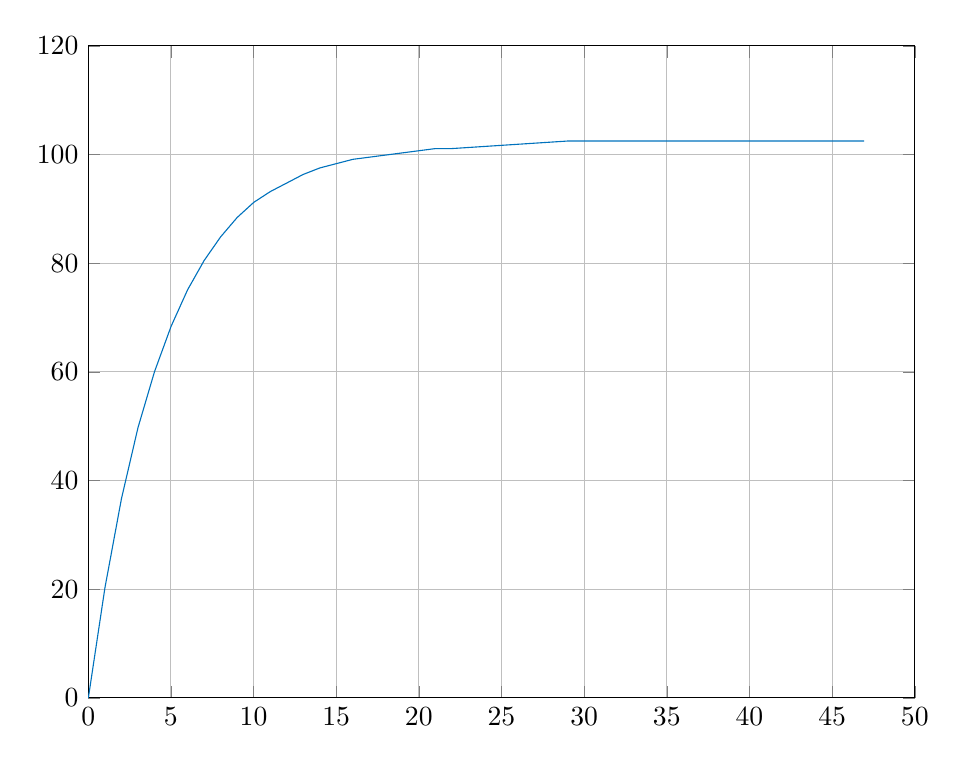
\begin{tikzpicture}

\begin{axis}[%
width=4.133in,
height=3.26in,
at={(0.693in,0.44in)},
scale only axis,
xmin=0,
xmax=50,
xmajorgrids,
ymin=0,
ymax=120,
ymajorgrids,
axis background/.style={fill=white}
]
\addplot [color=mycolor1,solid,forget plot]
  table[row sep=crcr]{%
0	0\\
0.0183688510000007	0.148\\
0.0333085550000006	0.46\\
0.048411227	0.764\\
0.0639306670000004	1.07\\
0.0799534620000003	1.394\\
0.0982038640000001	1.738\\
0.113255477	2.054\\
0.129045015000001	2.37\\
0.144356604	2.7\\
0.160402016	3.014\\
0.176073557	3.338\\
0.192149266	3.654\\
0.207947832	3.976\\
0.224124653	4.298\\
0.240001415	4.624\\
0.258240871	4.962\\
0.273553052	5.29\\
0.288614695	5.604\\
0.303944158	5.922\\
0.320296693	6.242\\
0.335924479	6.562\\
0.351968467	6.884\\
0.36793271	7.226\\
0.383990255	7.542\\
0.400113327000001	7.864\\
0.416061725	8.188\\
0.431937103	8.51\\
0.448054973000001	8.826\\
0.464105932	9.15\\
0.480011931	9.474\\
0.495890924000001	9.794\\
0.511894759	10.118\\
0.527906796	10.444\\
0.543917324000001	10.766\\
0.560083946	11.086\\
0.576077847000001	11.418\\
0.59203282	11.744\\
0.608008648	12.066\\
0.624084515000001	12.386\\
0.639994899	12.718\\
0.656079034	13.038\\
0.672099871000001	13.36\\
0.688106198000001	13.68\\
0.704106083000001	14.004\\
0.720049961000001	14.324\\
0.737160905000001	14.658\\
0.75250126	14.976\\
0.768142632999999	15.296\\
0.784054700999999	15.62\\
0.800066662	15.942\\
0.816106512	16.28\\
0.832087467	16.6\\
0.848028142000001	16.934\\
0.864095890000001	17.246\\
0.880003707	17.564\\
0.895955854	17.884\\
0.912117295	18.206\\
0.928327515000001	18.53\\
0.94397923	18.852\\
0.960180325000001	19.182\\
0.975936496000001	19.502\\
0.992044641000001	19.822\\
1.007965717	20.17\\
1.025603044	20.448\\
1.040587064	20.714\\
1.055945238	20.958\\
1.071973249	21.222\\
1.088018248	21.486\\
1.104082485	21.744\\
1.120156196	22.004\\
1.136085195	22.274\\
1.15203761	22.534\\
1.168089246	22.794\\
1.183971525	23.052\\
1.20000799	23.308\\
1.216084537	23.576\\
1.232158268	23.838\\
1.248273158	24.1\\
1.264076497	24.362\\
1.280082419	24.626\\
1.295884334	24.886\\
1.311956217	25.16\\
1.328067363	25.418\\
1.343973684	25.682\\
1.362448324	25.952\\
1.377668245	26.206\\
1.39320529	26.47\\
1.408662147	26.732\\
1.424079043	26.994\\
1.440028938	27.252\\
1.456163462	27.514\\
1.47205731	27.778\\
1.488080376	28.04\\
1.504082985	28.3\\
1.520143854	28.566\\
1.536009798	28.826\\
1.551891741	29.092\\
1.568081102	29.352\\
1.58403343	29.614\\
1.600087923	29.886\\
1.616054049	30.15\\
1.632332509	30.41\\
1.64787439	30.682\\
1.663894055	30.938\\
1.682074156	31.206\\
1.697872969	31.462\\
1.713137161	31.718\\
1.72905725	31.982\\
1.744443844	32.244\\
1.760382785	32.502\\
1.776001737	32.766\\
1.79198464	33.028\\
1.808005687	33.292\\
1.823902869	33.56\\
1.840012486	33.832\\
1.856109415	34.092\\
1.872084489	34.356\\
1.88811905	34.616\\
1.904166907	34.876\\
1.920054249	35.14\\
1.93609603	35.396\\
1.95207469	35.658\\
1.968200148	35.918\\
1.984080652	36.178\\
2.000057727	36.452\\
2.018331214	36.732\\
2.033306471	36.918\\
2.048307169	37.118\\
2.06397708	37.334\\
2.079933969	37.536\\
2.09609529	37.74\\
2.111932893	37.946\\
2.128148251	38.156\\
2.144043012	38.37\\
2.160125172	38.578\\
2.176089027	38.786\\
2.192050899	39.002\\
2.208037105	39.212\\
2.224094719	39.42\\
2.24005804	39.63\\
2.25615572	39.832\\
2.272046136	40.048\\
2.287893629	40.254\\
2.304042884	40.46\\
2.320069238	40.67\\
2.336075429	40.878\\
2.352039902	41.086\\
2.368128457	41.294\\
2.384037896	41.506\\
2.400017871	41.712\\
2.415924876	41.926\\
2.432140656	42.134\\
2.448063229	42.342\\
2.464108537	42.55\\
2.480163408	42.76\\
2.49610458	42.978\\
2.511973046	43.182\\
2.528025899	43.39\\
2.544106219	43.598\\
2.560032788	43.806\\
2.576003506	44.018\\
2.592085312	44.226\\
2.608035492	44.444\\
2.624093357	44.652\\
2.640164633	44.858\\
2.656125198	45.062\\
2.672063636	45.274\\
2.688164912	45.484\\
2.704155984	45.692\\
2.720072408	45.9\\
2.735890672	46.116\\
2.751870225	46.324\\
2.770154442	46.536\\
2.785357205	46.746\\
2.800494094	46.95\\
2.816019383	47.158\\
2.831984091	47.376\\
2.84801048	47.58\\
2.864075236	47.788\\
2.880054037	48.004\\
2.896098667	48.208\\
2.912052281	48.424\\
2.92830805	48.632\\
2.943932698	48.838\\
2.962417852	49.052\\
2.977686605	49.256\\
2.993616154	49.462\\
3.009400128	49.688\\
3.024228897	49.862\\
3.039919044	50.018\\
3.055970422	50.172\\
3.072866972	50.338\\
3.088017962	50.5\\
3.103887564	50.674\\
3.122308995	50.844\\
3.137616851	51.008\\
3.15272901	51.166\\
3.168100655	51.33\\
3.184029334	51.494\\
3.199968419	51.658\\
3.216020495	51.822\\
3.231953555	51.992\\
3.248110497	52.154\\
3.263919455	52.32\\
3.280095441	52.482\\
3.295897938	52.646\\
3.312112208	52.808\\
3.328019257	52.978\\
3.343933061	53.14\\
3.362431593	53.312\\
3.377549549	53.474\\
3.392731611	53.64\\
3.408218288	53.8\\
3.424109054	53.966\\
3.440044197	54.136\\
3.456041296	54.3\\
3.472079682	54.462\\
3.487968319	54.628\\
3.504038273	54.788\\
3.52001526	54.956\\
3.536047006	55.124\\
3.551888667	55.286\\
3.568106449	55.452\\
3.584043487	55.618\\
3.599998716	55.78\\
3.616067418	55.952\\
3.632058405	56.112\\
3.647991444	56.278\\
3.664075518	56.44\\
3.680088987	56.604\\
3.696110265	56.768\\
3.711984378	56.932\\
3.728077151	57.098\\
3.744062864	57.264\\
3.760323144	57.428\\
3.776031968	57.596\\
3.79224752	57.762\\
3.807954044	57.926\\
3.824078595	58.09\\
3.840019811	58.252\\
3.856091728	58.418\\
3.872047732	58.588\\
3.888169813	58.752\\
3.904113394	58.92\\
3.920077547	59.084\\
3.936080613	59.244\\
3.95203981	59.406\\
3.968056302	59.57\\
3.984052371	59.738\\
4.000004398	59.902\\
4.018208214	60.082\\
4.033212486	60.202\\
4.048166475	60.33\\
4.064010347	60.466\\
4.079990957	60.592\\
4.096028618	60.73\\
4.112078592	60.864\\
4.128132431	60.996\\
4.143971702	61.126\\
4.160019531	61.258\\
4.17614748	61.39\\
4.191983176	61.522\\
4.207888943	61.656\\
4.223927622	61.788\\
4.240118776	61.922\\
4.256063164	62.054\\
4.272131016	62.188\\
4.288157781	62.322\\
4.303899792	62.454\\
4.319992519	62.588\\
4.335995337	62.722\\
4.351890621	62.856\\
4.368105944	62.986\\
4.384069225	63.122\\
4.400005215	63.254\\
4.41599692	63.386\\
4.432103555	63.518\\
4.448007406	63.656\\
4.464065191	63.788\\
4.48006946	63.92\\
4.496049149	64.054\\
4.511983417	64.19\\
4.528015837	64.318\\
4.544052921	64.45\\
4.56006316	64.586\\
4.575976969	64.72\\
4.594297816	64.858\\
4.60952331	64.99\\
4.624655478	65.122\\
4.640127572	65.252\\
4.656043469	65.386\\
4.672049046	65.518\\
4.688105975	65.65\\
4.704036732	65.784\\
4.720056104	65.916\\
4.736126759	66.05\\
4.752065218	66.186\\
4.768082827	66.32\\
4.786409216	66.46\\
4.801569694	66.592\\
4.816685244	66.72\\
4.834282191	66.854\\
4.849399359	66.986\\
4.864709135	67.118\\
4.88004093	67.25\\
4.896132682	67.384\\
4.912002772	67.516\\
4.928146943	67.648\\
4.944013909	67.782\\
4.960076093	67.916\\
4.976096887	68.05\\
4.992139772	68.184\\
5.008023704	68.322\\
5.025551546	68.438\\
5.040541056	68.54\\
5.057022025	68.644\\
5.072017541	68.752\\
5.087905034	68.858\\
5.103991766	68.972\\
5.120173717	69.078\\
5.136090723	69.184\\
5.152037045	69.292\\
5.168383835	69.4\\
5.184074633	69.51\\
5.200121724	69.614\\
5.216306035	69.722\\
5.231952102	69.836\\
5.248089578	69.94\\
5.264073466	70.048\\
5.280074507	70.154\\
5.296065462	70.262\\
5.31211182	70.372\\
5.327936899	70.478\\
5.343977022	70.584\\
5.36001477	70.692\\
5.376059974	70.802\\
5.392059386	70.91\\
5.407962161	71.02\\
5.426280871	71.128\\
5.441475148	71.234\\
5.456669825	71.34\\
5.47207129	71.45\\
5.488115472	71.554\\
5.504112655	71.662\\
5.52001728	71.772\\
5.536034135	71.884\\
5.551886293	71.99\\
5.568101255	72.094\\
5.584075205	72.204\\
5.600033854	72.312\\
5.616000594	72.418\\
5.632115113	72.526\\
5.648068546	72.638\\
5.66412602	72.746\\
5.680021578	72.852\\
5.696071084	72.962\\
5.712007269	73.068\\
5.728144057	73.174\\
5.744016768	73.282\\
5.760161989	73.388\\
5.77604668	73.5\\
5.791877804	73.604\\
5.808132852	73.712\\
5.824030179	73.822\\
5.840030689	73.928\\
5.856093851	74.034\\
5.872014465	74.148\\
5.888196542	74.256\\
5.904041825	74.36\\
5.920048815	74.47\\
5.936071972	74.574\\
5.952065726	74.682\\
5.968085974	74.792\\
5.984032891	74.898\\
6.000202233	75.012\\
6.018186355	75.12\\
6.03338491	75.2\\
6.048346837	75.282\\
6.0639643	75.374\\
6.079958767	75.458\\
6.09595861	75.54\\
6.11203414	75.624\\
6.128358149	75.71\\
6.144016052	75.8\\
6.160255485	75.884\\
6.176036272	75.972\\
6.19202431	76.06\\
6.208006085	76.144\\
6.224127201	76.23\\
6.240026174	76.314\\
6.256046619	76.404\\
6.272057904	76.488\\
6.288042101	76.576\\
6.306266292	76.668\\
6.321504176	76.75\\
6.337771502	76.836\\
6.35283485	76.922\\
6.368079376	77.008\\
6.384074635	77.094\\
6.400105294	77.178\\
6.416045873	77.266\\
6.431980675	77.352\\
6.448071499	77.436\\
6.464009703	77.52\\
6.479961941	77.61\\
6.496096232	77.698\\
6.512043722	77.78\\
6.528107449	77.866\\
6.543868977	77.954\\
6.562184757	78.044\\
6.575885431	78.126\\
6.591889997	78.212\\
6.608178933	78.302\\
6.623943859	78.39\\
6.639935844	78.472\\
6.655927785	78.56\\
6.673989082	78.646\\
6.689320048	78.732\\
6.705154509	78.82\\
6.720247033	78.906\\
6.736071867	78.992\\
6.75208027	79.078\\
6.767923657	79.162\\
6.783989989	79.252\\
6.80228187	79.338\\
6.817631854	79.426\\
6.83292104	79.508\\
6.848212199	79.596\\
6.863970204	79.68\\
6.882241634	79.77\\
6.897894523	79.852\\
6.913187308	79.942\\
6.928397195	80.024\\
6.943943465	80.11\\
6.960045764	80.2\\
6.975865267	80.286\\
6.992126842	80.37\\
7.008050062	80.464\\
7.025718561	80.538\\
7.040718043	80.602\\
7.055940243	80.67\\
7.071948798	80.74\\
7.087987307	80.808\\
7.104052907	80.88\\
7.122582546	80.952\\
7.137761084	81.022\\
7.153741457	81.09\\
7.169128938	81.16\\
7.184402068	81.228\\
7.200038639	81.306\\
7.216094895	81.374\\
7.232001192	81.442\\
7.247924525	81.51\\
7.263997788	81.578\\
7.279947433	81.652\\
7.29610655	81.72\\
7.311906688	81.788\\
7.328099093	81.858\\
7.344035714	81.924\\
7.360078154	81.998\\
7.376295936	82.066\\
7.392145454	82.136\\
7.408146892	82.206\\
7.424092768	82.274\\
7.4401449	82.342\\
7.456162766	82.414\\
7.472180955	82.488\\
7.487989538	82.554\\
7.504052046	82.622\\
7.520150598	82.692\\
7.536059701	82.762\\
7.551890963	82.83\\
7.568041244	82.906\\
7.584021531	82.972\\
7.600051739	83.042\\
7.616059897	83.112\\
7.632000233	83.184\\
7.64813051	83.252\\
7.66397409	83.32\\
7.680095258	83.39\\
7.696049388	83.458\\
7.712115707	83.53\\
7.728077525	83.6\\
7.744041996	83.668\\
7.760215445	83.74\\
7.776069825	83.81\\
7.791990826	83.882\\
7.808134334	83.95\\
7.824046704	84.018\\
7.840095769	84.09\\
7.855989495	84.16\\
7.872103104	84.23\\
7.888161931	84.298\\
7.904082796	84.368\\
7.920141037	84.436\\
7.936030756	84.508\\
7.952107764	84.576\\
7.968144938	84.646\\
7.984028749	84.718\\
8.000027491	84.784\\
8.018456827	84.866\\
8.033437375	84.914\\
8.048477631	84.966\\
8.064010218	85.026\\
8.07994802	85.082\\
8.096082749	85.14\\
8.11207047	85.196\\
8.128055801	85.252\\
8.143977615	85.308\\
8.159942048	85.366\\
8.176176762	85.42\\
8.19207699	85.478\\
8.208061404	85.536\\
8.224100676	85.594\\
8.240084774	85.65\\
8.256079355	85.706\\
8.272108372	85.766\\
8.288100128	85.824\\
8.304109482	85.882\\
8.320065606	85.936\\
8.3360119	85.996\\
8.352021506	86.052\\
8.368085553	86.106\\
8.384090028	86.166\\
8.399968159	86.22\\
8.416119491	86.278\\
8.432133188	86.338\\
8.448053146	86.398\\
8.464013871	86.45\\
8.480101691	86.508\\
8.496117539	86.564\\
8.512068657	86.62\\
8.528063444	86.676\\
8.544035171	86.734\\
8.560087818	86.792\\
8.575965249	86.85\\
8.59203178	86.906\\
8.608116555	86.964\\
8.624039102	87.02\\
8.640096362	87.078\\
8.656076661	87.136\\
8.672148608	87.192\\
8.688113748	87.25\\
8.704000399	87.306\\
8.722291093	87.366\\
8.737598975	87.422\\
8.752907863	87.478\\
8.768171965	87.534\\
8.78403743	87.592\\
8.800054517	87.65\\
8.816091375	87.708\\
8.832031724	87.764\\
8.848089619	87.818\\
8.864099894	87.878\\
8.879898027	87.934\\
8.898206015	87.996\\
8.913419803	88.05\\
8.928649112	88.106\\
8.944309163	88.164\\
8.960117152	88.218\\
8.976113348	88.278\\
8.992105735	88.336\\
9.008041317	88.392\\
9.025565869	88.442\\
9.040568971	88.484\\
9.055918399	88.524\\
9.074044499	88.576\\
9.089062155	88.616\\
9.104111355	88.66\\
9.120202733	88.704\\
9.135847764	88.75\\
9.154227715	88.796\\
9.169592449	88.836\\
9.185173654	88.886\\
9.200428054	88.928\\
9.216112278	88.974\\
9.232056891	89.014\\
9.248059466	89.064\\
9.264056213	89.104\\
9.280137476	89.148\\
9.296011707	89.194\\
9.312128554	89.234\\
9.327894031	89.284\\
9.343915928	89.326\\
9.359887763	89.37\\
9.376304508	89.414\\
9.392086278	89.462\\
9.408083651	89.504\\
9.423885897	89.55\\
9.440069387	89.594\\
9.456174895	89.636\\
9.472077017	89.686\\
9.488045807	89.726\\
9.504014724	89.772\\
9.520117387	89.814\\
9.536080361	89.86\\
9.552060696	89.904\\
9.568192643	89.946\\
9.584067228	89.994\\
9.600080837	90.034\\
9.616080571	90.084\\
9.632037027	90.124\\
9.64808969	90.17\\
9.663998389	90.214\\
9.680021239	90.254\\
9.695972707	90.304\\
9.712047666	90.348\\
9.728037642	90.394\\
9.744155183	90.434\\
9.760088205	90.482\\
9.776757711	90.526\\
9.792659794	90.572\\
9.80796135	90.614\\
9.824096941	90.654\\
9.840061966	90.704\\
9.856077841	90.746\\
9.872187674	90.794\\
9.888370271	90.836\\
9.904031688	90.88\\
9.92011963	90.924\\
9.936064576	90.97\\
9.952094924	91.014\\
9.968010534	91.056\\
9.984115427	91.104\\
10.000072841	91.146\\
10.018405755	91.196\\
10.033374081	91.224\\
10.048361309	91.254\\
10.063925623	91.284\\
10.079977202	91.314\\
10.0959517	91.346\\
10.11209461	91.378\\
10.128112962	91.41\\
10.14433672	91.442\\
10.160114831	91.474\\
10.176203033	91.504\\
10.191977526	91.534\\
10.208055864	91.568\\
10.224019291	91.6\\
10.240103365	91.634\\
10.256086281	91.666\\
10.272034549	91.696\\
10.288105831	91.726\\
10.304008559	91.76\\
10.32000401	91.79\\
10.33607941	91.822\\
10.35208228	91.854\\
10.368062094	91.884\\
10.384037708	91.916\\
10.399997806	91.952\\
10.415891448	91.982\\
10.434147298	92.014\\
10.449389917	92.044\\
10.464664212	92.076\\
10.480136195	92.108\\
10.496101596	92.14\\
10.512095791	92.172\\
10.528197194	92.202\\
10.544061562	92.234\\
10.560095223	92.266\\
10.576334027	92.298\\
10.592086089	92.33\\
10.608046754	92.362\\
10.624091295	92.392\\
10.640059148	92.424\\
10.656090181	92.454\\
10.672056451	92.488\\
10.688069155	92.522\\
10.704008368	92.552\\
10.720175028	92.582\\
10.736127685	92.614\\
10.752067162	92.646\\
10.768036176	92.68\\
10.784152183	92.712\\
10.800027295	92.742\\
10.816082722	92.774\\
10.832081304	92.806\\
10.848106229	92.838\\
10.864075845	92.87\\
10.880158672	92.902\\
10.896064783	92.932\\
10.912086145	92.964\\
10.928081253	92.994\\
10.944318274	93.028\\
10.960121783	93.06\\
10.976326932	93.092\\
10.992006523	93.122\\
11.0080013	93.156\\
11.025378684	93.18\\
11.040376159	93.21\\
11.055933491	93.23\\
11.074081523	93.26\\
11.089123683	93.28\\
11.104067792	93.31\\
11.120133505	93.332\\
11.136045394	93.36\\
11.152107304	93.38\\
11.168079777	93.41\\
11.18399414	93.432\\
11.20004298	93.46\\
11.216071723	93.484\\
11.232033611	93.51\\
11.248089247	93.538\\
11.264040791	93.56\\
11.280025518	93.59\\
11.295892011	93.61\\
11.314057309	93.64\\
11.329015801	93.66\\
11.344009383	93.69\\
11.359944392	93.712\\
11.375946781	93.74\\
11.392062978	93.762\\
11.408266544	93.79\\
11.42408148	93.816\\
11.440146109	93.84\\
11.456099853	93.868\\
11.472118214	93.89\\
11.488105617	93.92\\
11.504024906	93.942\\
11.520034221	93.97\\
11.535874884	93.99\\
11.554183783	94.02\\
11.569170447	94.042\\
11.584171723	94.07\\
11.59991692	94.094\\
11.616103331	94.12\\
11.63203882	94.148\\
11.648111382	94.17\\
11.664049792	94.198\\
11.680107852	94.22\\
11.696196627	94.25\\
11.712079884	94.272\\
11.728120944	94.3\\
11.744190912	94.32\\
11.760110975	94.35\\
11.776241434	94.37\\
11.792006339	94.4\\
11.808070405	94.42\\
11.82391062	94.45\\
11.840137259	94.476\\
11.855973512	94.5\\
11.872005195	94.526\\
11.888007556	94.55\\
11.904073667	94.578\\
11.920119215	94.6\\
11.935884137	94.63\\
11.954200807	94.652\\
11.969444648	94.68\\
11.984568127	94.7\\
12.000080963	94.73\\
12.018308108	94.758\\
12.033291633	94.78\\
12.048267951	94.804\\
12.063930746	94.83\\
12.079955243	94.856\\
12.096045491	94.88\\
12.112087836	94.908\\
12.128143221	94.93\\
12.144338367	94.96\\
12.160052403	94.982\\
12.176227731	95.01\\
12.192011332	95.03\\
12.208090902	95.06\\
12.224000306	95.08\\
12.240152174	95.11\\
12.256107622	95.134\\
12.272180541	95.16\\
12.289087141	95.188\\
12.304143534	95.21\\
12.319975945	95.236\\
12.335990792	95.26\\
12.352122821	95.288\\
12.368020383	95.31\\
12.384121135	95.34\\
12.400066309	95.36\\
12.416090824	95.39\\
12.431956683	95.412\\
12.448094591	95.44\\
12.46404176	95.464\\
12.480085964	95.49\\
12.496019614	95.516\\
12.512104149	95.54\\
12.52796677	95.564\\
12.544008104	95.59\\
12.560054898	95.62\\
12.576305451	95.64\\
12.592105035	95.67\\
12.608132307	95.69\\
12.624008253	95.72\\
12.640036001	95.74\\
12.65607096	95.77\\
12.672085016	95.79\\
12.68809701	95.82\\
12.704186057	95.84\\
12.72025265	95.87\\
12.73603565	95.898\\
12.752101387	95.92\\
12.768061065	95.948\\
12.78403421	95.97\\
12.79996568	96\\
12.816018772	96.022\\
12.832095772	96.05\\
12.848049201	96.07\\
12.863974919	96.1\\
12.879994583	96.122\\
12.896119099	96.15\\
12.912144415	96.172\\
12.928095919	96.2\\
12.944102907	96.224\\
12.959964465	96.25\\
12.975945288	96.278\\
12.993129587	96.3\\
13.008829587	96.33\\
13.026328072	96.35\\
13.041608908	96.368\\
13.057149056	96.388\\
13.072211544	96.406\\
13.08821511	96.422\\
13.1040371	96.44\\
13.120026195	96.46\\
13.135931169	96.48\\
13.152232144	96.5\\
13.168052772	96.518\\
13.184101667	96.538\\
13.199986184	96.558\\
13.215908564	96.578\\
13.232115089	96.596\\
13.24813843	96.612\\
13.263986836	96.632\\
13.280096454	96.652\\
13.296047911	96.67\\
13.312143614	96.69\\
13.328115249	96.708\\
13.344163292	96.728\\
13.360135184	96.748\\
13.376402667	96.766\\
13.392589307	96.784\\
13.409157862	96.804\\
13.424421011	96.824\\
13.440025529	96.842\\
13.455966592	96.86\\
13.472122998	96.88\\
13.488089952	96.898\\
13.50407206	96.918\\
13.520166879	96.938\\
13.536107394	96.956\\
13.553903076	96.976\\
13.569270033	96.996\\
13.58452683	97.012\\
13.600041683	97.03\\
13.615960599	97.05\\
13.632071672	97.07\\
13.648105307	97.09\\
13.66400126	97.108\\
13.679966004	97.128\\
13.696039374	97.15\\
13.712056222	97.166\\
13.727982176	97.184\\
13.74388713	97.202\\
13.762161107	97.222\\
13.777414329	97.242\\
13.792662485	97.26\\
13.808122947	97.28\\
13.824074175	97.298\\
13.840156772	97.318\\
13.856084687	97.338\\
13.872073323	97.356\\
13.888114162	97.374\\
13.904062053	97.392\\
13.920029496	97.41\\
13.936069022	97.43\\
13.952077636	97.45\\
13.968068529	97.47\\
13.984112227	97.488\\
14.000077011	97.508\\
14.021658944	97.528\\
14.033776989	97.538\\
14.048971564	97.55\\
14.064151972	97.564\\
14.080082739	97.576\\
14.096079165	97.588\\
14.111954885	97.598\\
14.127983047	97.614\\
14.146452604	97.626\\
14.161545208	97.638\\
14.176746748	97.652\\
14.193127113	97.666\\
14.208377274	97.678\\
14.224087656	97.69\\
14.240058631	97.702\\
14.256061041	97.716\\
14.272094655	97.728\\
14.288037008	97.74\\
14.304051043	97.752\\
14.319986458	97.766\\
14.33605132	97.778\\
14.351989841	97.79\\
14.368031581	97.806\\
14.384109647	97.818\\
14.400104539	97.828\\
14.416066527	97.842\\
14.432042437	97.856\\
14.44791576	97.868\\
14.464054417	97.878\\
14.480303603	97.892\\
14.496056951	97.906\\
14.512053347	97.918\\
14.528033847	97.93\\
14.544033306	97.944\\
14.560068608	97.958\\
14.576332506	97.968\\
14.592149429	97.982\\
14.608079214	97.996\\
14.624112409	98.006\\
14.640082159	98.018\\
14.658217872	98.034\\
14.673464524	98.046\\
14.688761816	98.058\\
14.704003782	98.068\\
14.720194429	98.082\\
14.736028902	98.096\\
14.752112446	98.108\\
14.768022456	98.118\\
14.784235387	98.134\\
14.799879686	98.146\\
14.816046315	98.158\\
14.83194389	98.172\\
14.848077476	98.186\\
14.864065282	98.198\\
14.880101759	98.208\\
14.896034617	98.222\\
14.912053808	98.236\\
14.92800523	98.248\\
14.944266453	98.26\\
14.960087908	98.274\\
14.976287221	98.286\\
14.992705078	98.298\\
15.008171858	98.312\\
15.026031547	98.326\\
15.041078616	98.336\\
15.056212334	98.348\\
15.072114697	98.364\\
15.087996085	98.376\\
15.104228327	98.388\\
15.120056448	98.398\\
15.135974303	98.412\\
15.15218251	98.426\\
15.168078228	98.438\\
15.184083358	98.448\\
15.200037861	98.464\\
15.216144813	98.476\\
15.232057803	98.488\\
15.248123801	98.502\\
15.264193253	98.514\\
15.279983584	98.528\\
15.295883841	98.538\\
15.311948992	98.552\\
15.327913678	98.566\\
15.343923984	98.578\\
15.359868792	98.588\\
15.378277783	98.604\\
15.393496592	98.616\\
15.408752721	98.628\\
15.424126522	98.642\\
15.439966263	98.656\\
15.456036015	98.666\\
15.472152938	98.68\\
15.488126768	98.692\\
15.504246238	98.706\\
15.520001445	98.718\\
15.536053454	98.728\\
15.552074135	98.742\\
15.568034524	98.756\\
15.584048811	98.768\\
15.600006908	98.778\\
15.616114603	98.794\\
15.632042328	98.808\\
15.647991154	98.818\\
15.664015656	98.832\\
15.680146672	98.844\\
15.696100683	98.856\\
15.712140937	98.868\\
15.728044487	98.882\\
15.746526748	98.896\\
15.761945419	98.908\\
15.777243508	98.92\\
15.792601092	98.934\\
15.808000558	98.946\\
15.824047644	98.958\\
15.840125564	98.968\\
15.856011801	98.984\\
15.87206927	98.996\\
15.887985038	99.008\\
15.906436465	99.024\\
15.921817151	99.036\\
15.937268666	99.046\\
15.95250635	99.058\\
15.968099983	99.072\\
15.98408341	99.086\\
16.000033045	99.098\\
16.019160772	99.11\\
16.032070861	99.116\\
16.047950421	99.12\\
16.064059656	99.128\\
16.079979152	99.136\\
16.095955863	99.14\\
16.112008051	99.146\\
16.127974299	99.154\\
16.144211065	99.16\\
16.159953291	99.166\\
16.176204252	99.172\\
16.192008755	99.178\\
16.208059557	99.186\\
16.224041641	99.19\\
16.239967441	99.196\\
16.2560357	99.206\\
16.272085246	99.21\\
16.288009649	99.216\\
16.304268996	99.224\\
16.320112515	99.23\\
16.336049246	99.236\\
16.352118377	99.24\\
16.368062665	99.248\\
16.384100399	99.256\\
16.400039164	99.26\\
16.415905155	99.268\\
16.432038321	99.274\\
16.448083251	99.28\\
16.464002112	99.286\\
16.480063565	99.292\\
16.495973104	99.298\\
16.512272175	99.306\\
16.528064233	99.31\\
16.54410943	99.318\\
16.560020803	99.326\\
16.576095432	99.33\\
16.592006636	99.336\\
16.608131927	99.344\\
16.623921351	99.35\\
16.640018506	99.356\\
16.65587196	99.362\\
16.671922535	99.368\\
16.688033103	99.376\\
16.704273892	99.38\\
16.720145265	99.386\\
16.736015581	99.396\\
16.752101444	99.4\\
16.768044153	99.406\\
16.783983009	99.414\\
16.799973296	99.42\\
16.816089643	99.426\\
16.832052814	99.432\\
16.847976177	99.438\\
16.864055714	99.446\\
16.880134697	99.45\\
16.8960682	99.456\\
16.912202809	99.466\\
16.927988643	99.47\\
16.944314695	99.476\\
16.960026963	99.484\\
16.976195142	99.488\\
16.99200729	99.496\\
17.007993784	99.502\\
17.024039507	99.508\\
17.039916763	99.516\\
17.05607475	99.52\\
17.072240064	99.526\\
17.088102689	99.536\\
17.104174483	99.54\\
17.120067505	99.546\\
17.135995201	99.552\\
17.152065172	99.558\\
17.168019809	99.566\\
17.184004992	99.57\\
17.200055638	99.578\\
17.216090424	99.586\\
17.232048534	99.59\\
17.248068048	99.596\\
17.264147643	99.604\\
17.280050306	99.61\\
17.295882453	99.616\\
17.314005619	99.624\\
17.32923869	99.628\\
17.344601115	99.636\\
17.359974494	99.64\\
17.376140642	99.646\\
17.39196678	99.656\\
17.408035314	99.66\\
17.424012807	99.666\\
17.440038397	99.674\\
17.456094703	99.68\\
17.4720571	99.686\\
17.48805083	99.692\\
17.5042742	99.698\\
17.5200809	99.706\\
17.535932084	99.712\\
17.55428642	99.716\\
17.569387392	99.726\\
17.584582433	99.73\\
17.600132242	99.736\\
17.615927609	99.744\\
17.632068929	99.75\\
17.64809296	99.756\\
17.664035995	99.76\\
17.680121483	99.77\\
17.696032901	99.776\\
17.711998422	99.78\\
17.728014298	99.786\\
17.74438901	99.794\\
17.760033078	99.8\\
17.776110848	99.806\\
17.792230062	99.812\\
17.808112317	99.818\\
17.824066622	99.826\\
17.839987086	99.83\\
17.856013763	99.838\\
17.871946753	99.846\\
17.888089334	99.85\\
17.904110458	99.856\\
17.919946757	99.864\\
17.935995933	99.87\\
17.951922463	99.876\\
17.967969661	99.882\\
17.984104741	99.888\\
18.000042354	99.896\\
18.018661637	99.902\\
18.03393537	99.908\\
18.049139241	99.916\\
18.06421122	99.92\\
18.080157826	99.926\\
18.095921635	99.934\\
18.111956488	99.94\\
18.128070841	99.946\\
18.144100843	99.952\\
18.160067361	99.958\\
18.176072322	99.966\\
18.192008452	99.97\\
18.207894441	99.976\\
18.224031826	99.986\\
18.240088559	99.99\\
18.255945224	99.996\\
18.272043849	100.004\\
18.288187723	100.008\\
18.304225694	100.016\\
18.319979197	100.022\\
18.338144405	100.028\\
18.353388632	100.036\\
18.368685694	100.04\\
18.385926168	100.046\\
18.401264949	100.054\\
18.416769812	100.06\\
18.432070967	100.066\\
18.448175278	100.072\\
18.464050569	100.078\\
18.480119098	100.086\\
18.496058275	100.09\\
18.511924205	100.098\\
18.52814654	100.106\\
18.544009012	100.11\\
18.560110449	100.116\\
18.576289979	100.124\\
18.591956296	100.13\\
18.608061686	100.136\\
18.624045313	100.142\\
18.640011425	100.148\\
18.656035308	100.156\\
18.672082825	100.16\\
18.68793446	100.166\\
18.704150892	100.176\\
18.720110817	100.18\\
18.736021903	100.186\\
18.751881791	100.194\\
18.7678851	100.2\\
18.784104607	100.206\\
18.79992235	100.212\\
18.816038035	100.218\\
18.832030272	100.226\\
18.848089107	100.23\\
18.864149183	100.236\\
18.880072002	100.246\\
18.895961443	100.25\\
18.912073229	100.256\\
18.928090725	100.264\\
18.944031888	100.27\\
18.959962204	100.276\\
18.976158718	100.282\\
18.992004307	100.288\\
19.008185971	100.296\\
19.025573896	100.3\\
19.0412209	100.306\\
19.056318062	100.316\\
19.072227348	100.32\\
19.087925621	100.326\\
19.104166508	100.332\\
19.119916739	100.338\\
19.135850792	100.346\\
19.154169908	100.352\\
19.169308541	100.358\\
19.184418173	100.366\\
19.200025553	100.37\\
19.216122004	100.376\\
19.232050041	100.384\\
19.247997237	100.39\\
19.264037078	100.396\\
19.279972581	100.402\\
19.296055778	100.408\\
19.314533459	100.416\\
19.329742691	100.42\\
19.344987813	100.426\\
19.360292237	100.436\\
19.376003727	100.44\\
19.392059122	100.446\\
19.408037647	100.454\\
19.423992775	100.46\\
19.43996003	100.466\\
19.455970413	100.472\\
19.472088003	100.478\\
19.488185655	100.486\\
19.504078594	100.49\\
19.520072996	100.496\\
19.5361104	100.506\\
19.551931428	100.51\\
19.567888699	100.516\\
19.584126956	100.524\\
19.600038347	100.53\\
19.616055456	100.536\\
19.632039944	100.542\\
19.648112092	100.548\\
19.6640722	100.556\\
19.679990411	100.56\\
19.696210577	100.566\\
19.712227061	100.574\\
19.728084495	100.58\\
19.744294824	100.586\\
19.760063177	100.594\\
19.776087426	100.6\\
19.792016867	100.606\\
19.808085707	100.61\\
19.824029249	100.618\\
19.840014527	100.626\\
19.856051171	100.63\\
19.872124456	100.636\\
19.888036929	100.644\\
19.904201072	100.65\\
19.920024154	100.656\\
19.936031473	100.662\\
19.952138348	100.668\\
19.967962173	100.676\\
19.984093248	100.68\\
19.999984341	100.688\\
20.018235427	100.696\\
20.033398976	100.7\\
20.048479309	100.706\\
20.064103367	100.714\\
20.080060498	100.72\\
20.096034048	100.726\\
20.112224814	100.732\\
20.127986443	100.738\\
20.143986276	100.746\\
20.159981733	100.75\\
20.17629535	100.756\\
20.191998826	100.766\\
20.208061538	100.77\\
20.223980448	100.776\\
20.239969492	100.784\\
20.256054504	100.79\\
20.272159972	100.796\\
20.287967588	100.8\\
20.306222091	100.808\\
20.321433374	100.816\\
20.336587557	100.82\\
20.352152305	100.826\\
20.368015543	100.836\\
20.384078445	100.84\\
20.400042363	100.846\\
20.416095913	100.852\\
20.43206209	100.858\\
20.448153637	100.866\\
20.464152219	100.87\\
20.480013522	100.878\\
20.496097552	100.886\\
20.512152031	100.89\\
20.528082706	100.896\\
20.54396704	100.904\\
20.559968864	100.91\\
20.576131594	100.916\\
20.592072915	100.922\\
20.608044715	100.928\\
20.623994312	100.936\\
20.640304624	100.94\\
20.65589583	100.946\\
20.671875286	100.956\\
20.688083964	100.96\\
20.704099283	100.966\\
20.72014689	100.974\\
20.736018315	100.98\\
20.752060788	100.986\\
20.76803986	100.992\\
20.784088864	100.998\\
20.800041997	101.006\\
20.816140715	101.01\\
20.832077976	101.016\\
20.848087718	101.026\\
20.86403155	101.03\\
20.879896504	101.036\\
20.896036108	101.044\\
20.912068512	101.05\\
20.928018422	101.056\\
20.944086309	101.062\\
20.960040379	101.068\\
20.976085297	101.076\\
20.992071939	101.08\\
21.008075045	101.086\\
21.026015658	101.088\\
21.041163116	101.088\\
21.056209224	101.088\\
21.072067163	101.088\\
21.088009917	101.088\\
21.104185023	101.088\\
21.119975772	101.088\\
21.136008317	101.088\\
21.152069373	101.088\\
21.168069337	101.088\\
21.184081514	101.088\\
21.200044283	101.088\\
21.215987813	101.088\\
21.232074149	101.088\\
21.248084544	101.088\\
21.264099575	101.088\\
21.280093801	101.088\\
21.298414903	101.088\\
21.313482647	101.088\\
21.328762004	101.088\\
21.34489592	101.088\\
21.360044223	101.088\\
21.376062795	101.088\\
21.39203227	101.088\\
21.408168296	101.088\\
21.423936554	101.088\\
21.440129151	101.088\\
21.456051875	101.088\\
21.472107886	101.088\\
21.488080395	101.088\\
21.50398275	101.088\\
21.520112969	101.088\\
21.535884545	101.088\\
21.552121117	101.088\\
21.568065559	101.088\\
21.58411713	101.088\\
21.600049254	101.088\\
21.616118772	101.088\\
21.632026667	101.088\\
21.648058353	101.088\\
21.664078477	101.088\\
21.680072523	101.088\\
21.695937271	101.088\\
21.711969888	101.088\\
21.728046075	101.088\\
21.746503731	101.088\\
21.761785909	101.088\\
21.776991583	101.088\\
21.792411076	101.088\\
21.808087965	101.088\\
21.823874124	101.088\\
21.839897309	101.088\\
21.855972726	101.088\\
21.872094822	101.088\\
21.888049028	101.088\\
21.904145946	101.088\\
21.920020395	101.088\\
21.936095003	101.088\\
21.952077267	101.088\\
21.968175289	101.088\\
21.984522513	101.088\\
22.000060619	101.088\\
22.018158303	101.09\\
22.033488012	101.094\\
22.048459011	101.096\\
22.06404852	101.1\\
22.080208227	101.104\\
22.09608663	101.106\\
22.112081747	101.11\\
22.127969462	101.114\\
22.144040038	101.116\\
22.159943269	101.12\\
22.176284829	101.122\\
22.192049064	101.124\\
22.208085811	101.126\\
22.224080315	101.132\\
22.240054203	101.134\\
22.256076923	101.136\\
22.272092778	101.14\\
22.288024352	101.144\\
22.303894411	101.146\\
22.319981029	101.15\\
22.336093601	101.154\\
22.352103953	101.156\\
22.368042533	101.16\\
22.384133739	101.164\\
22.400096143	101.166\\
22.416215634	101.17\\
22.43200576	101.174\\
22.448049384	101.176\\
22.464051201	101.18\\
22.480144111	101.182\\
22.496142106	101.186\\
22.512058495	101.188\\
22.528260246	101.192\\
22.544052714	101.194\\
22.559998541	101.196\\
22.576205793	101.202\\
22.59202278	101.204\\
22.607954685	101.206\\
22.623980337	101.21\\
22.640096123	101.214\\
22.656147829	101.216\\
22.672006703	101.22\\
22.688092874	101.224\\
22.704107891	101.226\\
22.720036563	101.23\\
22.738238104	101.234\\
22.753421225	101.236\\
22.76872533	101.24\\
22.784146561	101.244\\
22.800052194	101.246\\
22.815987516	101.25\\
22.832189616	101.252\\
22.84791287	101.254\\
22.864010956	101.256\\
22.880110702	101.262\\
22.895954744	101.264\\
22.912075966	101.266\\
22.928008061	101.27\\
22.943982398	101.274\\
22.960190773	101.276\\
22.976028864	101.28\\
22.992021959	101.284\\
23.008131977	101.286\\
23.025820927	101.29\\
23.04107414	101.294\\
23.056149461	101.296\\
23.072064682	101.3\\
23.088100804	101.304\\
23.104092356	101.306\\
23.120149976	101.31\\
23.136090602	101.312\\
23.152052242	101.316\\
23.168067276	101.318\\
23.184064588	101.322\\
23.200077361	101.324\\
23.216502654	101.326\\
23.23207552	101.332\\
23.248070994	101.334\\
23.264068116	101.336\\
23.279893054	101.34\\
23.295915107	101.344\\
23.312080723	101.346\\
23.328028642	101.35\\
23.344059687	101.354\\
23.36011691	101.356\\
23.375963578	101.36\\
23.392144782	101.364\\
23.408058055	101.366\\
23.424065177	101.37\\
23.440034139	101.374\\
23.456076664	101.376\\
23.47203507	101.38\\
23.48807329	101.384\\
23.504108017	101.384\\
23.52008727	101.386\\
23.536001023	101.392\\
23.552084193	101.394\\
23.568030427	101.396\\
23.584004623	101.4\\
23.600078771	101.404\\
23.616058318	101.406\\
23.632081138	101.41\\
23.64786872	101.414\\
23.663912769	101.416\\
23.680007689	101.42\\
23.696097208	101.424\\
23.712067994	101.426\\
23.728103458	101.43\\
23.744002408	101.434\\
23.762446153	101.436\\
23.777752265	101.44\\
23.79294696	101.442\\
23.808178215	101.446\\
23.823994065	101.448\\
23.840097929	101.452\\
23.856091849	101.454\\
23.872027203	101.456\\
23.88808883	101.462\\
23.904036009	101.464\\
23.920043415	101.466\\
23.936391688	101.47\\
23.953060914	101.474\\
23.96850362	101.476\\
23.984046886	101.48\\
24.000091119	101.484\\
24.01924402	101.486\\
24.031987124	101.49\\
24.048000035	101.494\\
24.063955726	101.496\\
24.079938336	101.5\\
24.095971888	101.504\\
24.112097251	101.506\\
24.128193418	101.51\\
24.144026022	101.512\\
24.160093605	101.514\\
24.176117257	101.516\\
24.192122037	101.522\\
24.208310098	101.524\\
24.224084976	101.526\\
24.240132252	101.532\\
24.256771867	101.534\\
24.272087256	101.536\\
24.287924669	101.54\\
24.303897846	101.544\\
24.319947608	101.546\\
24.336100735	101.55\\
24.352015556	101.554\\
24.368112743	101.556\\
24.384091659	101.56\\
24.400086574	101.564\\
24.415877955	101.566\\
24.434031032	101.57\\
24.4491764	101.574\\
24.464329225	101.576\\
24.479885865	101.58\\
24.496056185	101.582\\
24.512110732	101.584\\
24.527953367	101.586\\
24.544158403	101.592\\
24.560313754	101.594\\
24.576072041	101.596\\
24.592137047	101.6\\
24.608088235	101.604\\
24.624014751	101.606\\
24.640121275	101.61\\
24.656074551	101.614\\
24.672078307	101.616\\
24.688209901	101.62\\
24.704135702	101.624\\
24.720134483	101.626\\
24.736009484	101.63\\
24.751987293	101.634\\
24.768068486	101.636\\
24.783994126	101.64\\
24.802276965	101.642\\
24.817502456	101.644\\
24.833007354	101.646\\
24.848220926	101.652\\
24.864036227	101.654\\
24.880026582	101.656\\
24.895984966	101.66\\
24.912219835	101.664\\
24.928119056	101.666\\
24.943955361	101.67\\
24.962368003	101.674\\
24.977481494	101.676\\
24.992552804	101.68\\
25.008080839	101.684\\
25.025675821	101.686\\
25.040792011	101.69\\
25.055937519	101.694\\
25.072087079	101.696\\
25.088087555	101.7\\
25.104077821	101.704\\
25.120078347	101.706\\
25.136050905	101.708\\
25.151984235	101.712\\
25.168174616	101.714\\
25.18413209	101.716\\
25.20031128	101.722\\
25.216024649	101.724\\
25.232086518	101.726\\
25.247967571	101.73\\
25.264088636	101.734\\
25.280238258	101.736\\
25.295959289	101.74\\
25.312104339	101.744\\
25.328104708	101.746\\
25.344075678	101.75\\
25.360279959	101.754\\
25.376085432	101.756\\
25.392064854	101.76\\
25.408016775	101.764\\
25.424062637	101.766\\
25.440082532	101.77\\
25.456103849	101.774\\
25.472074973	101.774\\
25.488068627	101.776\\
25.504167705	101.782\\
25.52006643	101.784\\
25.535954338	101.786\\
25.552033594	101.792\\
25.568072271	101.794\\
25.584056026	101.796\\
25.600076453	101.8\\
25.61606208	101.804\\
25.632117624	101.806\\
25.648039907	101.81\\
25.663905129	101.814\\
25.679935421	101.816\\
25.695930657	101.82\\
25.712066915	101.824\\
25.728234744	101.826\\
25.744106327	101.83\\
25.760151911	101.832\\
25.776063184	101.836\\
25.791923722	101.84\\
25.810169382	101.842\\
25.825448352	101.844\\
25.841544433	101.846\\
25.856699839	101.852\\
25.872095759	101.854\\
25.888066358	101.856\\
25.904177037	101.86\\
25.920049271	101.864\\
25.936082697	101.866\\
25.952057845	101.87\\
25.968136562	101.874\\
25.984037517	101.876\\
26.000069926	101.88\\
26.018211514	101.884\\
26.033439168	101.886\\
26.048739727	101.89\\
26.063888513	101.894\\
26.080091317	101.896\\
26.09607858	101.9\\
26.112110225	101.902\\
26.12811996	101.904\\
26.144066954	101.908\\
26.160177863	101.912\\
26.176072609	101.914\\
26.192019265	101.916\\
26.208018115	101.922\\
26.224130803	101.924\\
26.240076179	101.926\\
26.256079544	101.93\\
26.271955447	101.934\\
26.288078711	101.936\\
26.304180452	101.94\\
26.320053525	101.944\\
26.336054488	101.946\\
26.352036066	101.95\\
26.368081403	101.954\\
26.384115063	101.956\\
26.399984062	101.96\\
26.416038312	101.964\\
26.432126626	101.966\\
26.448072903	101.968\\
26.464097155	101.972\\
26.480050696	101.974\\
26.496074273	101.976\\
26.512056773	101.982\\
26.530439384	101.984\\
26.545791745	101.986\\
26.560926177	101.992\\
26.576256032	101.994\\
26.592206676	101.996\\
26.608086359	102\\
26.624074501	102.004\\
26.640089815	102.006\\
26.656105349	102.01\\
26.672067798	102.014\\
26.68808425	102.016\\
26.704085992	102.02\\
26.720046532	102.024\\
26.736082429	102.026\\
26.752033255	102.03\\
26.768067502	102.032\\
26.784167021	102.034\\
26.800222656	102.036\\
26.816195408	102.042\\
26.832074303	102.044\\
26.848106786	102.046\\
26.864077754	102.052\\
26.879996108	102.054\\
26.896049137	102.056\\
26.912090539	102.06\\
26.928131131	102.064\\
26.944000008	102.066\\
26.95999141	102.07\\
26.976112897	102.074\\
26.99451382	102.076\\
27.00982589	102.08\\
27.025727631	102.084\\
27.041169454	102.086\\
27.057428988	102.09\\
27.071966897	102.094\\
27.088005103	102.096\\
27.104206596	102.098\\
27.119951497	102.102\\
27.136073167	102.104\\
27.152078603	102.106\\
27.16791146	102.112\\
27.184122044	102.114\\
27.200108754	102.116\\
27.216056119	102.12\\
27.232119691	102.124\\
27.247997289	102.126\\
27.264101288	102.13\\
27.280071194	102.134\\
27.296055177	102.136\\
27.312470707	102.14\\
27.327896901	102.144\\
27.343874722	102.146\\
27.360224525	102.15\\
27.376030241	102.154\\
27.391993894	102.156\\
27.408049502	102.16\\
27.423995481	102.162\\
27.440051745	102.164\\
27.456151645	102.168\\
27.47206122	102.172\\
27.488077467	102.174\\
27.504081879	102.176\\
27.520108599	102.182\\
27.5360765	102.184\\
27.552030545	102.186\\
27.568369778	102.19\\
27.584122787	102.194\\
27.600804916	102.196\\
27.616107025	102.2\\
27.632123471	102.204\\
27.648198844	102.206\\
27.664109186	102.21\\
27.680069019	102.214\\
27.696073759	102.216\\
27.712085565	102.22\\
27.728165272	102.224\\
27.743990903	102.226\\
27.762433766	102.228\\
27.777745331	102.232\\
27.792980933	102.234\\
27.808147164	102.236\\
27.824062731	102.242\\
27.839994257	102.244\\
27.85618221	102.246\\
27.872089219	102.25\\
27.888035542	102.254\\
27.904112379	102.256\\
27.92013558	102.26\\
27.936200411	102.264\\
27.9520649	102.266\\
27.968112954	102.27\\
27.984047329	102.274\\
28.00012428	102.276\\
28.018312195	102.28\\
28.032070823	102.284\\
28.047931665	102.286\\
28.064097624	102.29\\
28.079986739	102.292\\
28.096131295	102.296\\
28.11210098	102.298\\
28.128130557	102.302\\
28.144113838	102.304\\
28.160331825	102.306\\
28.176159685	102.312\\
28.19208533	102.314\\
28.208080784	102.316\\
28.224043959	102.32\\
28.240073827	102.324\\
28.256099182	102.326\\
28.271970131	102.33\\
28.28822913	102.334\\
28.303947989	102.336\\
28.320041684	102.34\\
28.336029564	102.344\\
28.352071424	102.346\\
28.368123826	102.35\\
28.384089332	102.354\\
28.400050348	102.356\\
28.41592413	102.36\\
28.432132683	102.362\\
28.448001978	102.364\\
28.464073261	102.366\\
28.480132001	102.372\\
28.496098507	102.374\\
28.512116679	102.376\\
28.528066224	102.38\\
28.544068591	102.384\\
28.560277528	102.386\\
28.575907348	102.39\\
28.594288101	102.394\\
28.60942962	102.396\\
28.624585126	102.4\\
28.640030008	102.404\\
28.656076393	102.406\\
28.672702385	102.41\\
28.688100574	102.414\\
28.704079165	102.416\\
28.720085722	102.42\\
28.736043377	102.422\\
28.752041662	102.424\\
28.768080384	102.426\\
28.784088687	102.432\\
28.799908908	102.434\\
28.816191505	102.436\\
28.831943892	102.442\\
28.847873589	102.444\\
28.863970223	102.446\\
28.879931395	102.45\\
28.896067331	102.454\\
28.912068594	102.456\\
28.928100069	102.46\\
28.944093237	102.464\\
28.960240173	102.466\\
28.976105363	102.47\\
28.99232086	102.474\\
29.008094759	102.474\\
29.025572679	102.474\\
29.041499492	102.474\\
29.056647766	102.474\\
29.072175937	102.474\\
29.087890915	102.474\\
29.104089454	102.474\\
29.120144528	102.474\\
29.136083619	102.474\\
29.152098041	102.474\\
29.168074955	102.474\\
29.184060143	102.474\\
29.200086642	102.474\\
29.216061348	102.474\\
29.231955916	102.474\\
29.248265166	102.474\\
29.264140488	102.474\\
29.280038112	102.474\\
29.295881591	102.474\\
29.312378802	102.474\\
29.32808617	102.474\\
29.344030226	102.474\\
29.360278332	102.474\\
29.376155127	102.474\\
29.392164372	102.474\\
29.411405706	102.474\\
29.424667021	102.474\\
29.439902203	102.474\\
29.456131177	102.474\\
29.472085543	102.474\\
29.488215521	102.474\\
29.504099783	102.474\\
29.520000383	102.474\\
29.536029031	102.474\\
29.552111231	102.474\\
29.568114264	102.474\\
29.584078178	102.474\\
29.600172121	102.474\\
29.615996221	102.474\\
29.632200683	102.474\\
29.648094608	102.474\\
29.664028025	102.474\\
29.679979955	102.474\\
29.695979253	102.474\\
29.712043272	102.474\\
29.728224442	102.474\\
29.744013779	102.474\\
29.760048324	102.474\\
29.776090912	102.474\\
29.792119274	102.474\\
29.80804948	102.474\\
29.824138666	102.474\\
29.840020983	102.474\\
29.85615446	102.474\\
29.871959465	102.474\\
29.890530095	102.474\\
29.904084111	102.474\\
29.920006757	102.474\\
29.936087308	102.474\\
29.952029842	102.474\\
29.96810671	102.474\\
29.984073649	102.474\\
30.000118831	102.474\\
30.01846943	102.474\\
30.034081328	102.474\\
30.049513748	102.474\\
30.064680213	102.474\\
30.079926177	102.474\\
30.095889678	102.474\\
30.112090455	102.474\\
30.128140392	102.474\\
30.144248583	102.474\\
30.160323547	102.474\\
30.176179086	102.474\\
30.192105384	102.474\\
30.208035023	102.474\\
30.224087551	102.474\\
30.240068332	102.474\\
30.256110717	102.474\\
30.272034979	102.474\\
30.287985062	102.474\\
30.304132954	102.474\\
30.32006314	102.474\\
30.336034176	102.474\\
30.352063138	102.474\\
30.368090564	102.474\\
30.384097324	102.474\\
30.400069434	102.474\\
30.416157824	102.474\\
30.432084686	102.474\\
30.448081085	102.474\\
30.464201767	102.474\\
30.480066518	102.474\\
30.496108623	102.474\\
30.512077546	102.474\\
30.528203702	102.474\\
30.543959074	102.474\\
30.560159261	102.474\\
30.576089897	102.474\\
30.592102123	102.474\\
30.60808632	102.474\\
30.624056828	102.474\\
30.640079112	102.474\\
30.656093303	102.474\\
30.672079537	102.474\\
30.688064095	102.474\\
30.704094723	102.474\\
30.720101693	102.474\\
30.736098475	102.474\\
30.752097156	102.474\\
30.768067087	102.474\\
30.784165719	102.474\\
30.799933065	102.474\\
30.816113649	102.474\\
30.832071017	102.474\\
30.848031523	102.474\\
30.864100652	102.474\\
30.88003404	102.474\\
30.896125707	102.474\\
30.912208824	102.474\\
30.928196706	102.474\\
30.944109151	102.474\\
30.960198583	102.474\\
30.976090242	102.474\\
30.992135741	102.474\\
31.008040718	102.474\\
31.026087009	102.474\\
31.041281275	102.474\\
31.056461683	102.474\\
31.072095287	102.474\\
31.088165966	102.474\\
31.104174354	102.474\\
31.120093525	102.474\\
31.136476727	102.474\\
31.152056905	102.474\\
31.168119631	102.474\\
31.184023949	102.474\\
31.199960339	102.474\\
31.216058645	102.474\\
31.232075678	102.474\\
31.248019979	102.474\\
31.264378186	102.474\\
31.280153993	102.474\\
31.296000382	102.474\\
31.312004751	102.474\\
31.327984609	102.474\\
31.344026775	102.474\\
31.360091927	102.474\\
31.37605633	102.474\\
31.392116996	102.474\\
31.408044629	102.474\\
31.424077963	102.474\\
31.440108484	102.474\\
31.456108619	102.474\\
31.472071233	102.474\\
31.488075001	102.474\\
31.503891274	102.474\\
31.520170981	102.474\\
31.53598981	102.474\\
31.551894754	102.474\\
31.568045295	102.474\\
31.584111964	102.474\\
31.60010825	102.474\\
31.615891177	102.474\\
31.632033994	102.474\\
31.648021615	102.474\\
31.664143365	102.474\\
31.680048026	102.474\\
31.69610897	102.474\\
31.712035037	102.474\\
31.72808548	102.474\\
31.74407042	102.474\\
31.760386985	102.474\\
31.776050323	102.474\\
31.791992086	102.474\\
31.807928775	102.474\\
31.824058112	102.474\\
31.83996634	102.474\\
31.856176543	102.474\\
31.872046904	102.474\\
31.888090298	102.474\\
31.903977928	102.474\\
31.920181679	102.474\\
31.93608523	102.474\\
31.952040078	102.474\\
31.968117608	102.474\\
31.984034459	102.474\\
32.000058488	102.474\\
32.018467859	102.474\\
32.033542031	102.474\\
32.048612935	102.474\\
32.063997948	102.474\\
32.08007937	102.474\\
32.096031059	102.474\\
32.112019575	102.474\\
32.128186069	102.474\\
32.144073352	102.474\\
32.160360402	102.474\\
32.176030042	102.474\\
32.192062645	102.474\\
32.207966523	102.474\\
32.224124418	102.474\\
32.240090345	102.474\\
32.255994831	102.474\\
32.272042023	102.474\\
32.287889067	102.474\\
32.306230409	102.474\\
32.321595734	102.474\\
32.336890555	102.474\\
32.352306935	102.474\\
32.36807176	102.474\\
32.384035777	102.474\\
32.400056024	102.474\\
32.415893801	102.474\\
32.431949925	102.474\\
32.448000691	102.474\\
32.464133294	102.474\\
32.480097306	102.474\\
32.496101199	102.474\\
32.511993326	102.474\\
32.528067419	102.474\\
32.543979176	102.474\\
32.560057904	102.474\\
32.576052029	102.474\\
32.592049861	102.474\\
32.607955195	102.474\\
32.624103331	102.474\\
32.640012418	102.474\\
32.656119881	102.474\\
32.672065206	102.474\\
32.688302132	102.474\\
32.704022943	102.474\\
32.720054143	102.474\\
32.73606872	102.474\\
32.752100133	102.474\\
32.768143004	102.474\\
32.783954153	102.474\\
32.800148106	102.474\\
32.816109112	102.474\\
32.832006782	102.474\\
32.84790603	102.474\\
32.864056936	102.474\\
32.879987275	102.474\\
32.896063725	102.474\\
32.91203558	102.474\\
32.927963979	102.474\\
32.944024327	102.474\\
32.960204661	102.474\\
32.976205376	102.474\\
32.992173558	102.474\\
33.00794676	102.474\\
33.025801932	102.474\\
33.040940531	102.474\\
33.056037785	102.474\\
33.071984687	102.474\\
33.088029339	102.474\\
33.104043581	102.474\\
33.119988334	102.474\\
33.136075226	102.474\\
33.152041589	102.474\\
33.168109968	102.474\\
33.184039056	102.474\\
33.20009628	102.474\\
33.216040457	102.474\\
33.232000137	102.474\\
33.248146896	102.474\\
33.264082574	102.474\\
33.280097041	102.474\\
33.29623352	102.474\\
33.311991349	102.474\\
33.328195236	102.474\\
33.344021712	102.474\\
33.360225375	102.474\\
33.376060166	102.474\\
33.39207494	102.474\\
33.408151001	102.474\\
33.424070002	102.474\\
33.440023156	102.474\\
33.456105199	102.474\\
33.472065975	102.474\\
33.488088409	102.474\\
33.504117291	102.474\\
33.520012354	102.474\\
33.536076765	102.474\\
33.551898861	102.474\\
33.568012087	102.474\\
33.583946923	102.474\\
33.600099207	102.474\\
33.61610345	102.474\\
33.632122858	102.474\\
33.647922133	102.474\\
33.664102018	102.474\\
33.680026588	102.474\\
33.696075447	102.474\\
33.712036258	102.474\\
33.728072343	102.474\\
33.744024885	102.474\\
33.760125892	102.474\\
33.77601928	102.474\\
33.791889525	102.474\\
33.808170481	102.474\\
33.824107271	102.474\\
33.840029976	102.474\\
33.856188323	102.474\\
33.872088922	102.474\\
33.888078959	102.474\\
33.903978718	102.474\\
33.920120391	102.474\\
33.936099712	102.474\\
33.952008864	102.474\\
33.968112795	102.474\\
33.984056457	102.474\\
34.000090959	102.474\\
34.018393644	102.474\\
34.033649407	102.474\\
34.048823263	102.474\\
34.064070307	102.474\\
34.080039126	102.474\\
34.096079096	102.474\\
34.112057035	102.474\\
34.128150491	102.474\\
34.144048379	102.474\\
34.160221926	102.474\\
34.176027118	102.474\\
34.192151053	102.474\\
34.208034689	102.474\\
34.223979991	102.474\\
34.240044028	102.474\\
34.256175414	102.474\\
34.271963626	102.474\\
34.287898219	102.474\\
34.304153106	102.474\\
34.320038138	102.474\\
34.336157008	102.474\\
34.352075262	102.474\\
34.368080994	102.474\\
34.383967675	102.474\\
34.400074943	102.474\\
34.416033088	102.474\\
34.43204351	102.474\\
34.448039561	102.474\\
34.46416683	102.474\\
34.479974078	102.474\\
34.496106935	102.474\\
34.51209646	102.474\\
34.528158935	102.474\\
34.543962635	102.474\\
34.560018081	102.474\\
34.576193863	102.474\\
34.592244533	102.474\\
34.607985031	102.474\\
34.624014936	102.474\\
34.640042154	102.474\\
34.656094051	102.474\\
34.671991929	102.474\\
34.688151454	102.474\\
34.704060693	102.474\\
34.7202059	102.474\\
34.736053625	102.474\\
34.751996357	102.474\\
34.767905668	102.474\\
34.784005998	102.474\\
34.799978215	102.474\\
34.815988111	102.474\\
34.83209191	102.474\\
34.848029613	102.474\\
34.864064306	102.474\\
34.880034227	102.474\\
34.896125758	102.474\\
34.912023746	102.474\\
34.927999555	102.474\\
34.943866488	102.474\\
34.962378442	102.474\\
34.977684143	102.474\\
34.992871416	102.474\\
35.008189937	102.474\\
35.025909621	102.474\\
35.041116425	102.474\\
35.056402625	102.474\\
35.072017282	102.474\\
35.088132562	102.474\\
35.105342707	102.474\\
35.120425906	102.474\\
35.135908255	102.474\\
35.152069219	102.474\\
35.168109299	102.474\\
35.184069884	102.474\\
35.200257718	102.474\\
35.21603363	102.474\\
35.232021935	102.474\\
35.247982289	102.474\\
35.264030786	102.474\\
35.280155637	102.474\\
35.295945195	102.474\\
35.312023623	102.474\\
35.329788584	102.474\\
35.344821219	102.474\\
35.360077476	102.474\\
35.376020973	102.474\\
35.39222588	102.474\\
35.408072807	102.474\\
35.424104192	102.474\\
35.439996828	102.474\\
35.456088671	102.474\\
35.471937938	102.474\\
35.488052662	102.474\\
35.504086572	102.474\\
35.52006222	102.474\\
35.536049256	102.474\\
35.554262137	102.474\\
35.569477614	102.474\\
35.5847102	102.474\\
35.600079861	102.474\\
35.616213775	102.474\\
35.632087557	102.474\\
35.648030983	102.474\\
35.664138966	102.474\\
35.680056233	102.474\\
35.696134771	102.474\\
35.712052793	102.474\\
35.727965489	102.474\\
35.743933689	102.474\\
35.76012121	102.474\\
35.775977384	102.474\\
35.791888912	102.474\\
35.810234775	102.474\\
35.825563503	102.474\\
35.840766066	102.474\\
35.856145479	102.474\\
35.872115218	102.474\\
35.888103991	102.474\\
35.904075212	102.474\\
35.92013871	102.474\\
35.936112344	102.474\\
35.95204829	102.474\\
35.96808053	102.474\\
35.984046557	102.474\\
36.000043785	102.474\\
36.01841923	102.474\\
36.033521621	102.474\\
36.048679397	102.474\\
36.064083732	102.474\\
36.080083833	102.474\\
36.095947511	102.474\\
36.111901351	102.474\\
36.128209929	102.474\\
36.143965113	102.474\\
36.160151375	102.474\\
36.176025478	102.474\\
36.19202278	102.474\\
36.208061188	102.474\\
36.224093078	102.474\\
36.240010229	102.474\\
36.256090825	102.474\\
36.272098172	102.474\\
36.288049636	102.474\\
36.304203659	102.474\\
36.320139499	102.474\\
36.336112423	102.474\\
36.35202683	102.474\\
36.368031946	102.474\\
36.384062153	102.474\\
36.400091093	102.474\\
36.416045719	102.474\\
36.4320773	102.474\\
36.448015023	102.474\\
36.464106394	102.474\\
36.480033793	102.474\\
36.496093903	102.474\\
36.512106902	102.474\\
36.52811297	102.474\\
36.543958657	102.474\\
36.56012199	102.474\\
36.576076694	102.474\\
36.591957032	102.474\\
36.607968678	102.474\\
36.624143423	102.474\\
36.640042854	102.474\\
36.656131534	102.474\\
36.672065218	102.474\\
36.688028398	102.474\\
36.704088102	102.474\\
36.722680324	102.474\\
36.737974955	102.474\\
36.753154846	102.474\\
36.768285957	102.474\\
36.784065952	102.474\\
36.800049124	102.474\\
36.815945832	102.474\\
36.83203947	102.474\\
36.847999948	102.474\\
36.864037774	102.474\\
36.880066167	102.474\\
36.89612069	102.474\\
36.911965826	102.474\\
36.928308938	102.474\\
36.944048994	102.474\\
36.960415572	102.474\\
36.976030691	102.474\\
36.992148742	102.474\\
37.007986515	102.474\\
37.025553604	102.474\\
37.040767969	102.474\\
37.056756644	102.474\\
37.072122762	102.474\\
37.088107629	102.474\\
37.104083568	102.474\\
37.120047173	102.474\\
37.136081195	102.474\\
37.152051508	102.474\\
37.168102788	102.474\\
37.18406481	102.474\\
37.200079455	102.474\\
37.216041401	102.474\\
37.23208718	102.474\\
37.248043744	102.474\\
37.264092479	102.474\\
37.280068643	102.474\\
37.296136674	102.474\\
37.312011403	102.474\\
37.328303094	102.474\\
37.344047377	102.474\\
37.360329971	102.474\\
37.376055744	102.474\\
37.392070045	102.474\\
37.407973213	102.474\\
37.424068755	102.474\\
37.440028227	102.474\\
37.456123327	102.474\\
37.47208542	102.474\\
37.488042091	102.474\\
37.504092639	102.474\\
37.520197736	102.474\\
37.536030487	102.474\\
37.551912235	102.474\\
37.568047341	102.474\\
37.583995475	102.474\\
37.599981085	102.474\\
37.616107802	102.474\\
37.631998591	102.474\\
37.647977358	102.474\\
37.664065147	102.474\\
37.679981449	102.474\\
37.696106083	102.474\\
37.712022653	102.474\\
37.728201322	102.474\\
37.744030203	102.474\\
37.760247372	102.474\\
37.776088784	102.474\\
37.791890555	102.474\\
37.808146217	102.474\\
37.823994048	102.474\\
37.839893302	102.474\\
37.855925332	102.474\\
37.871900608	102.474\\
37.887910948	102.474\\
37.904071803	102.474\\
37.919933086	102.474\\
37.936007133	102.474\\
37.95207643	102.474\\
37.96805905	102.474\\
37.984066947	102.474\\
38.000117756	102.474\\
38.018451125	102.474\\
38.033929814	102.474\\
38.049038503	102.474\\
38.0643214	102.474\\
38.08005803	102.474\\
38.095907728	102.474\\
38.11185315	102.474\\
38.128113849	102.474\\
38.144064782	102.474\\
38.160202684	102.474\\
38.176072066	102.474\\
38.192086734	102.474\\
38.208281659	102.474\\
38.224095963	102.474\\
38.240131728	102.474\\
38.256034973	102.474\\
38.272082264	102.474\\
38.288018711	102.474\\
38.30390082	102.474\\
38.319959134	102.474\\
38.335911861	102.474\\
38.351925945	102.474\\
38.368072281	102.474\\
38.384060738	102.474\\
38.400122556	102.474\\
38.416182547	102.474\\
38.432252725	102.474\\
38.448044288	102.474\\
38.464086788	102.474\\
38.48005752	102.474\\
38.495890595	102.474\\
38.512051384	102.474\\
38.528081946	102.474\\
38.544071289	102.474\\
38.560163751	102.474\\
38.576337629	102.474\\
38.592060455	102.474\\
38.607940795	102.474\\
38.62617128	102.474\\
38.64127807	102.474\\
38.656344474	102.474\\
38.672032742	102.474\\
38.68815569	102.474\\
38.703929767	102.474\\
38.722331261	102.474\\
38.737526652	102.474\\
38.752701733	102.474\\
38.768242682	102.474\\
38.784082032	102.474\\
38.800068155	102.474\\
38.816058021	102.474\\
38.832039092	102.474\\
38.848153921	102.474\\
38.864063751	102.474\\
38.880050581	102.474\\
38.896057139	102.474\\
38.911945834	102.474\\
38.927974116	102.474\\
38.944186472	102.474\\
38.960009514	102.474\\
38.978330303	102.474\\
38.993983181	102.474\\
39.009391504	102.474\\
39.024312229	102.474\\
39.039880058	102.474\\
39.0559695	102.474\\
39.072046273	102.474\\
39.088081994	102.474\\
39.104006158	102.474\\
39.120346511	102.474\\
39.136053636	102.474\\
39.152080857	102.474\\
39.167975564	102.474\\
39.18393664	102.474\\
39.200058854	102.474\\
39.216084862	102.474\\
39.232063212	102.474\\
39.248061598	102.474\\
39.264029808	102.474\\
39.279939321	102.474\\
39.295940345	102.474\\
39.312120457	102.474\\
39.328068654	102.474\\
39.344185888	102.474\\
39.360044637	102.474\\
39.376065944	102.474\\
39.392066264	102.474\\
39.408158888	102.474\\
39.424106885	102.474\\
39.440100795	102.474\\
39.456060081	102.474\\
39.472181736	102.474\\
39.488198102	102.474\\
39.504179674	102.474\\
39.520156145	102.474\\
39.536110014	102.474\\
39.552073473	102.474\\
39.568073916	102.474\\
39.583930144	102.474\\
39.600001916	102.474\\
39.616121947	102.474\\
39.632376307	102.474\\
39.648111646	102.474\\
39.664055313	102.474\\
39.680069002	102.474\\
39.69607043	102.474\\
39.712083569	102.474\\
39.728109186	102.474\\
39.744174794	102.474\\
39.760174407	102.474\\
39.776367134	102.474\\
39.791902657	102.474\\
39.808121569	102.474\\
39.824018477	102.474\\
39.839977585	102.474\\
39.856072014	102.474\\
39.872106932	102.474\\
39.888046625	102.474\\
39.904067997	102.474\\
39.920027364	102.474\\
39.936053948	102.474\\
39.952088811	102.474\\
39.968010217	102.474\\
39.984073179	102.474\\
40.000026437	102.474\\
40.018504685	102.474\\
40.033721369	102.474\\
40.049042967	102.474\\
40.064320475	102.474\\
40.07993069	102.474\\
40.09657756	102.474\\
40.111889795	102.474\\
40.13013479	102.474\\
40.145339725	102.474\\
40.160570473	102.474\\
40.176437082	102.474\\
40.192067363	102.474\\
40.208463974	102.474\\
40.224075209	102.474\\
40.240098255	102.474\\
40.256118931	102.474\\
40.27209458	102.474\\
40.288087375	102.474\\
40.304112203	102.474\\
40.320193155	102.474\\
40.33631491	102.474\\
40.352099165	102.474\\
40.368012252	102.474\\
40.384073721	102.474\\
40.400017347	102.474\\
40.416156116	102.474\\
40.431911447	102.474\\
40.448063027	102.474\\
40.463969817	102.474\\
40.480089826	102.474\\
40.496172838	102.474\\
40.511918687	102.474\\
40.528077019	102.474\\
40.544068769	102.474\\
40.559907071	102.474\\
40.575892373	102.474\\
40.592095618	102.474\\
40.608120358	102.474\\
40.624062746	102.474\\
40.639995109	102.474\\
40.656213941	102.474\\
40.671958587	102.474\\
40.688113237	102.474\\
40.70401042	102.474\\
40.720018851	102.474\\
40.736014961	102.474\\
40.752084608	102.474\\
40.768127223	102.474\\
40.784012738	102.474\\
40.799923297	102.474\\
40.816052827	102.474\\
40.832075808	102.474\\
40.848082959	102.474\\
40.864120693	102.474\\
40.880060561	102.474\\
40.896084676	102.474\\
40.912119191	102.474\\
40.928100433	102.474\\
40.944252141	102.474\\
40.960079208	102.474\\
40.976296545	102.474\\
40.992071884	102.474\\
41.008071352	102.474\\
41.025831759	102.474\\
41.041106485	102.474\\
41.056712286	102.474\\
41.072138285	102.474\\
41.08806368	102.474\\
41.104183515	102.474\\
41.1201132	102.474\\
41.135968614	102.474\\
41.152017746	102.474\\
41.167978762	102.474\\
41.184151599	102.474\\
41.200073686	102.474\\
41.216138722	102.474\\
41.231947012	102.474\\
41.248050537	102.474\\
41.264007161	102.474\\
41.280223236	102.474\\
41.295991893	102.474\\
41.311956426	102.474\\
41.330319043	102.474\\
41.34548786	102.474\\
41.360682415	102.474\\
41.376241543	102.474\\
41.392067736	102.474\\
41.408127685	102.474\\
41.424114745	102.474\\
41.439888939	102.474\\
41.455884708	102.474\\
41.472116075	102.474\\
41.487946842	102.474\\
41.50403384	102.474\\
41.520120432	102.474\\
41.535952729	102.474\\
41.55198107	102.474\\
41.568882451	102.474\\
41.584086542	102.474\\
41.600101898	102.474\\
41.616103643	102.474\\
41.632057072	102.474\\
41.64789798	102.474\\
41.663949797	102.474\\
41.680109613	102.474\\
41.696092959	102.474\\
41.712133971	102.474\\
41.728009274	102.474\\
41.744116134	102.474\\
41.760084276	102.474\\
41.776099389	102.474\\
41.791882582	102.474\\
41.807950682	102.474\\
41.824083941	102.474\\
41.840035636	102.474\\
41.856072308	102.474\\
41.872312757	102.474\\
41.88812942	102.474\\
41.904073793	102.474\\
41.91997668	102.474\\
41.936060245	102.474\\
41.952105918	102.474\\
41.968060534	102.474\\
41.984090606	102.474\\
42.000061369	102.474\\
42.018434744	102.474\\
42.033617162	102.474\\
42.048694801	102.474\\
42.064154178	102.474\\
42.080177788	102.474\\
42.096052646	102.474\\
42.112116733	102.474\\
42.128154337	102.474\\
42.144222726	102.474\\
42.160242637	102.474\\
42.17633768	102.474\\
42.192021016	102.474\\
42.208139789	102.474\\
42.224095568	102.474\\
42.240025664	102.474\\
42.256124667	102.474\\
42.272219641	102.474\\
42.288199119	102.474\\
42.304023949	102.474\\
42.320099052	102.474\\
42.336029864	102.474\\
42.352074583	102.474\\
42.368050337	102.474\\
42.384093161	102.474\\
42.400077211	102.474\\
42.416078068	102.474\\
42.431934838	102.474\\
42.448077002	102.474\\
42.464061501	102.474\\
42.480128076	102.474\\
42.496027502	102.474\\
42.512090539	102.474\\
42.527971293	102.474\\
42.544315737	102.474\\
42.560062077	102.474\\
42.57614219	102.474\\
42.59207086	102.474\\
42.608102225	102.474\\
42.624090302	102.474\\
42.640113338	102.474\\
42.656149395	102.474\\
42.671959831	102.474\\
42.688073089	102.474\\
42.704117528	102.474\\
42.719976308	102.474\\
42.736024365	102.474\\
42.752067873	102.474\\
42.768026388	102.474\\
42.784086127	102.474\\
42.800071576	102.474\\
42.815953224	102.474\\
42.831891213	102.474\\
42.850061772	102.474\\
42.864996636	102.474\\
42.88002688	102.474\\
42.896071322	102.474\\
42.911973645	102.474\\
42.92809271	102.474\\
42.944123027	102.474\\
42.960091862	102.474\\
42.976385423	102.474\\
42.992014594	102.474\\
43.008068569	102.474\\
43.025794123	102.474\\
43.04087711	102.474\\
43.055921029	102.474\\
43.072067127	102.474\\
43.088045718	102.474\\
43.104175245	102.474\\
43.120648787	102.474\\
43.136041234	102.474\\
43.152124622	102.474\\
43.168028863	102.474\\
43.18413763	102.474\\
43.199971386	102.474\\
43.215994723	102.474\\
43.23195512	102.474\\
43.247979767	102.474\\
43.264055163	102.474\\
43.280185537	102.474\\
43.296090366	102.474\\
43.312150401	102.474\\
43.328107688	102.474\\
43.344177722	102.474\\
43.359972114	102.474\\
43.37611873	102.474\\
43.392099491	102.474\\
43.408026388	102.474\\
43.424130043	102.474\\
43.440046466	102.474\\
43.456156636	102.474\\
43.472076158	102.474\\
43.488056671	102.474\\
43.504144767	102.474\\
43.520184	102.474\\
43.536133449	102.474\\
43.551891278	102.474\\
43.570154054	102.474\\
43.585333981	102.474\\
43.600652192	102.474\\
43.616155143	102.474\\
43.632086438	102.474\\
43.648075968	102.474\\
43.664036562	102.474\\
43.680087842	102.474\\
43.696073814	102.474\\
43.712097416	102.474\\
43.728137256	102.474\\
43.744086359	102.474\\
43.759980063	102.474\\
43.776300001	102.474\\
43.792105796	102.474\\
43.807882925	102.474\\
43.826098427	102.474\\
43.841291193	102.474\\
43.856647084	102.474\\
43.871886653	102.474\\
43.888066927	102.474\\
43.904074769	102.474\\
43.919996546	102.474\\
43.936105822	102.474\\
43.952086141	102.474\\
43.968024611	102.474\\
43.98394148	102.474\\
44.000025847	102.474\\
44.018376065	102.474\\
44.034018388	102.474\\
44.04792606	102.474\\
44.066128095	102.474\\
44.081205198	102.474\\
44.096404136	102.474\\
44.112031255	102.474\\
44.128076333	102.474\\
44.144111432	102.474\\
44.16016567	102.474\\
44.17604323	102.474\\
44.192144654	102.474\\
44.208031168	102.474\\
44.224036247	102.474\\
44.239891762	102.474\\
44.256005107	102.474\\
44.272034745	102.474\\
44.288004136	102.474\\
44.303947977	102.474\\
44.319904801	102.474\\
44.335970198	102.474\\
44.352070196	102.474\\
44.368066266	102.474\\
44.384102136	102.474\\
44.400048068	102.474\\
44.416077093	102.474\\
44.432091715	102.474\\
44.447969641	102.474\\
44.464057465	102.474\\
44.480100547	102.474\\
44.496029846	102.474\\
44.512079653	102.474\\
44.528081872	102.474\\
44.546406532	102.474\\
44.561641651	102.474\\
44.576843379	102.474\\
44.592146915	102.474\\
44.608044422	102.474\\
44.624035441	102.474\\
44.640036708	102.474\\
44.656040961	102.474\\
44.672049174	102.474\\
44.688037005	102.474\\
44.70408805	102.474\\
44.720348779	102.474\\
44.736043036	102.474\\
44.752151541	102.474\\
44.768029528	102.474\\
44.7840857	102.474\\
44.799873401	102.474\\
44.81614857	102.474\\
44.832039216	102.474\\
44.848072912	102.474\\
44.864044286	102.474\\
44.88003088	102.474\\
44.896110213	102.474\\
44.912095229	102.474\\
44.928199014	102.474\\
44.944301038	102.474\\
44.960055711	102.474\\
44.976326879	102.474\\
44.99202912	102.474\\
45.00806533	102.474\\
45.025556101	102.474\\
45.040722768	102.474\\
45.056118913	102.474\\
45.072043398	102.474\\
45.088093243	102.474\\
45.104088278	102.474\\
45.120750851	102.474\\
45.136149057	102.474\\
45.152072592	102.474\\
45.168100605	102.474\\
45.184115869	102.474\\
45.200058833	102.474\\
45.216120374	102.474\\
45.232023487	102.474\\
45.248194421	102.474\\
45.264042855	102.474\\
45.280104232	102.474\\
45.295928585	102.474\\
45.311960027	102.474\\
45.328095996	102.474\\
45.343953269	102.474\\
45.359934173	102.474\\
45.376070795	102.474\\
45.39195218	102.474\\
45.408029193	102.474\\
45.424132893	102.474\\
45.440461524	102.474\\
45.45635207	102.474\\
45.472078987	102.474\\
45.488118296	102.474\\
45.504174667	102.474\\
45.520359626	102.474\\
45.536069753	102.474\\
45.552098562	102.474\\
45.56809796	102.474\\
45.58408555	102.474\\
45.599960491	102.474\\
45.616076553	102.474\\
45.632017548	102.474\\
45.64808978	102.474\\
45.664077518	102.474\\
45.680078662	102.474\\
45.696148356	102.474\\
45.712092218	102.474\\
45.728101829	102.474\\
45.744186565	102.474\\
45.759901313	102.474\\
45.77600318	102.474\\
45.792058868	102.474\\
45.808057784	102.474\\
45.823993114	102.474\\
45.840122358	102.474\\
45.856112309	102.474\\
45.872125208	102.474\\
45.888078741	102.474\\
45.904032616	102.474\\
45.922543979	102.474\\
45.937820339	102.474\\
45.953106867	102.474\\
45.968477425	102.474\\
45.984121863	102.474\\
46.00000842	102.474\\
46.018429876	102.474\\
46.033696177	102.474\\
46.048781713	102.474\\
46.064112548	102.474\\
46.080123328	102.474\\
46.096024657	102.474\\
46.111999654	102.474\\
46.12805769	102.474\\
46.144135127	102.474\\
46.160202277	102.474\\
46.176318863	102.474\\
46.191956691	102.474\\
46.208112539	102.474\\
46.224059272	102.474\\
46.24015163	102.474\\
46.256048751	102.474\\
46.2721282	102.474\\
46.288018108	102.474\\
46.303937152	102.474\\
46.320095859	102.474\\
46.336052538	102.474\\
46.352111933	102.474\\
46.368091261	102.474\\
46.384048728	102.474\\
46.400030671	102.474\\
46.416044046	102.474\\
46.431881053	102.474\\
46.448070846	102.474\\
46.463882577	102.474\\
46.480126889	102.474\\
46.496032089	102.474\\
46.512065458	102.474\\
46.528234979	102.474\\
46.543993401	102.474\\
46.559912111	102.474\\
46.576154616	102.474\\
46.591892257	102.474\\
46.610015756	102.474\\
46.625055417	102.474\\
46.640157836	102.474\\
46.655971307	102.474\\
46.674298472	102.474\\
46.689413416	102.474\\
46.704489484	102.474\\
46.720139613	102.474\\
46.736013357	102.474\\
46.752072889	102.474\\
46.768045975	102.474\\
46.784106726	102.474\\
46.800111505	102.474\\
46.816042292	102.474\\
46.832187385	102.474\\
46.84796133	102.474\\
46.864038696	102.474\\
46.880023113	102.474\\
46.896070338	102.474\\
46.912098439	102.474\\
46.928057157	102.474\\
};
\end{axis}
\end{tikzpicture}%}
      \caption{The error in bearing of the robot over time for
        $(K_{\Psi}^R, K_{\omega}^T) \equiv (0.1 K_{\Psi, max}^R, 0.75 K_{\omega, max}^T)$}
      \label{fig:19_4_angle}
    \end{figure}
  \end{minipage}
\end{minipage}
}



\noindent\makebox[\textwidth][c]{%
\begin{minipage}{\linewidth}
  \begin{minipage}{0.45\linewidth}
    \begin{figure}[H]
      \scalebox{0.6}{% This file was created by matlab2tikz.
%
%The latest updates can be retrieved from
%  http://www.mathworks.com/matlabcentral/fileexchange/22022-matlab2tikz-matlab2tikz
%where you can also make suggestions and rate matlab2tikz.
%
\definecolor{mycolor1}{rgb}{0.00000,0.44700,0.74100}%
%
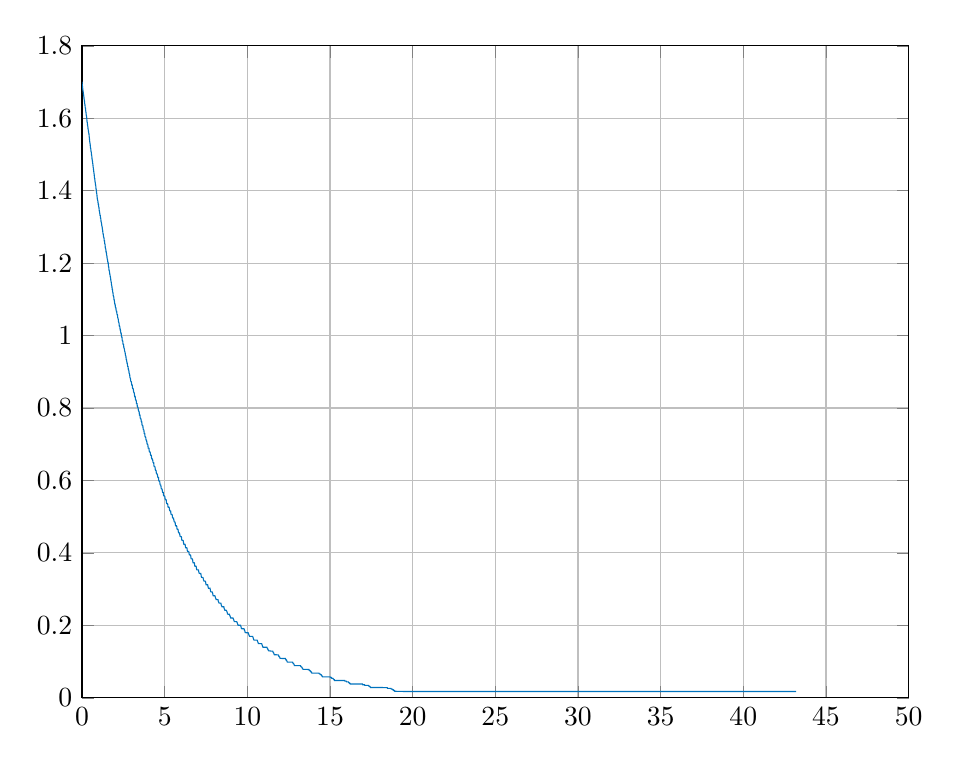
\begin{tikzpicture}

\begin{axis}[%
width=4.133in,
height=3.26in,
at={(0.693in,0.44in)},
scale only axis,
xmin=0,
xmax=50,
xmajorgrids,
ymin=0,
ymax=1.8,
ymajorgrids,
axis background/.style={fill=white}
]
\addplot [color=mycolor1,solid,forget plot]
  table[row sep=crcr]{%
0	1.70070137502122\\
0.0150263859999999	1.69086836645218\\
0.0310508189999983	1.68694825276524\\
0.047106237999998	1.67910941359981\\
0.0631314529999979	1.67518888235766\\
0.0792779730009995	1.66931010111042\\
0.0952288600009978	1.66343048690221\\
0.111220470999997	1.65951078862103\\
0.127221406000998	1.65167111649463\\
0.143358967	1.64971147613164\\
0.159183676999997	1.64027822955148\\
0.175062704999998	1.63791882719962\\
0.191183244999997	1.63007915507321\\
0.207090103000998	1.62811951471023\\
0.223258086999997	1.62027984258383\\
0.238996928999998	1.61635972889688\\
0.255097807	1.60852088973145\\
0.271256180999998	1.6065604164075\\
0.287224967999998	1.59872157724206\\
0.303064732000999	1.5912483885801\\
0.321278167999998	1.58692892831004\\
0.33637943	1.57908925618363\\
0.352108583999999	1.57712961582065\\
0.367110524000999	1.56928994369425\\
0.383221836999997	1.56733030333126\\
0.399035195999999	1.55949063120486\\
0.417372812999997	1.55753099084187\\
0.432501781000998	1.54969131871547\\
0.447765412000999	1.54417763057477\\
0.463008020999998	1.53593902942045\\
0.479174237	1.53201884599173\\
0.495857138	1.52613971693107\\
0.511271386	1.51830004480466\\
0.527037046999998	1.51634040444168\\
0.543367	1.50850073231528\\
0.559373543001	1.50654109195229\\
0.575063919000998	1.49870141982589\\
0.591195334999997	1.49554591464862\\
0.607062041000999	1.48690877089386\\
0.625229621999998	1.48298865720692\\
0.640427482000999	1.47710945840447\\
0.655604305999998	1.47318934471753\\
0.671171848999999	1.4653505055521\\
0.687137897000998	1.46143032212337\\
0.703052651	1.45555119306271\\
0.719111625	1.44967095171579\\
0.735188351	1.44455601575904\\
0.751021944001	1.43591887200428\\
0.767055976999998	1.43395923164129\\
0.784291217999998	1.42611955951489\\
0.799327373999998	1.42219944582795\\
0.815019684	1.4163202470255\\
0.833113220999997	1.41240013333856\\
0.848108011999998	1.40456129417313\\
0.863289062999997	1.40260082084917\\
0.879034967999998	1.39396177372338\\
0.895201538999997	1.39080817191715\\
0.911131890999999	1.38296933275171\\
0.927323467999998	1.3770897185435\\
0.944807386999998	1.37317002026233\\
0.959791704999998	1.37120954693837\\
0.975083079999998	1.36337070777294\\
0.991111937000997	1.36337070777294\\
1.00708324	1.35553103564653\\
1.023118533	1.35357139528355\\
1.039292129	1.34573172315715\\
1.055055816	1.3421785083404\\
1.071174807001	1.3378585629228\\
1.087251758001	1.33197943386213\\
1.103058108	1.33197943386213\\
1.119079553001	1.32413976173573\\
1.13518491	1.32218012137274\\
1.151158387	1.31434044924634\\
1.167240680001	1.31238080888336\\
1.183070422	1.30846062545463\\
1.199105916001	1.30258149639397\\
1.215540976	1.30062102307001\\
1.231048644	1.29394161630721\\
1.247183456001	1.29078884746194\\
1.263028664	1.28294917533554\\
1.279170359001	1.28098953497255\\
1.295116446	1.27510992076434\\
1.311032756	1.27119022248316\\
1.32918229	1.26922974915921\\
1.344242757999	1.26139090999378\\
1.35945863	1.26139090999378\\
1.375283085	1.25355123786737\\
1.391149468	1.25159159750439\\
1.407106514	1.24335113737866\\
1.423099078	1.23979894857236\\
1.439122092	1.23783847524841\\
1.455223893001	1.22999963608297\\
1.471083001	1.22999963608297\\
1.487189738	1.22215996395657\\
1.503062007	1.22020032359358\\
1.519046004	1.21236065146718\\
1.535005671	1.2104010111042\\
1.551694438	1.20648082767547\\
1.567040437	1.20060169861481\\
1.583170219	1.20060169861481\\
1.599008625	1.19156205653917\\
1.617208315	1.18880904968278\\
1.631048623001	1.18096937755638\\
1.64725563	1.17900973719339\\
1.663032329001	1.17508955376467\\
1.679286911	1.169210424704\\
1.695277676	1.16724995138005\\
1.711181968	1.1613707525776\\
1.727069255	1.15941111221461\\
1.743511887	1.15157144008821\\
1.759005161	1.14961179972523\\
1.777159165999	1.14293197755666\\
1.79222575	1.1378191507932\\
1.807236156001	1.13585867746924\\
1.823123088001	1.12801983830381\\
1.839090463	1.12801983830381\\
1.855236642001	1.12018016617741\\
1.871172187	1.11822052581442\\
1.88723717	1.11038085368802\\
1.903276282	1.10842121332503\\
1.919526874	1.10646074000108\\
1.934999975001	1.09862190083565\\
1.951057331001	1.09822111283632\\
1.967079179	1.09154168953949\\
1.983045839	1.08682925190362\\
2.001187592	1.08682925190362\\
2.016158013	1.07898957977722\\
2.031135198999	1.07702993941423\\
2.047214748001	1.07702993941423\\
2.063239502001	1.06919026728783\\
2.079079852001	1.06723062692484\\
2.095107581001	1.06723062692484\\
2.111122566	1.05939095479844\\
2.127119058001	1.05743131443545\\
2.143154251	1.05743131443545\\
2.159029455	1.04959164230905\\
2.175181225001	1.04723121394674\\
2.191239745	1.04487132066175\\
2.207050961	1.03819465023095\\
2.223175602001	1.03583935301404\\
2.239112462	1.03387887969008\\
2.255003308	1.02604004052465\\
2.271244408	1.02604004052465\\
2.287141037	1.02407956720069\\
2.302989091001	1.01624072803526\\
2.3190952	1.01624072803526\\
2.335105116001	1.01036048668835\\
2.351334552	1.00644141554587\\
2.367303743	1.00644141554587\\
2.38333648	0.998601743419472\\
2.399337316	0.996241315057155\\
2.415164362	0.995841895096126\\
2.431282092	0.987204751341372\\
2.447345755	0.984849454124458\\
2.463242214	0.984849454124458\\
2.479173892	0.977009781998056\\
2.495158140001	0.97505014163507\\
2.511243161	0.97505014163507\\
2.527164995	0.967210469508668\\
2.543110169001	0.965250829145682\\
2.559033782	0.963290355821726\\
2.577170217	0.95741115701928\\
2.592169825	0.955451516656293\\
2.607226327	0.953491043332338\\
2.623112286001	0.945652204166905\\
2.639030925001	0.944851996206546\\
2.655190359001	0.942094051254238\\
2.671242142001	0.933859555234878\\
2.687283575	0.933859555234878\\
2.703149304	0.929939371806154\\
2.719153301001	0.924060242745489\\
2.735132469	0.924060242745489\\
2.751159648	0.918180001398572\\
2.767278831001	0.914260930256101\\
2.783022803	0.914260930256101\\
2.799225548	0.906421258129699\\
2.815124923	0.904461617766713\\
2.830984357	0.904461617766713\\
2.84716266	0.896621945640311\\
2.863260384	0.894261517277994\\
2.879021354	0.893462335328085\\
2.895101336002	0.884829296708284\\
2.913498653	0.882869656345298\\
2.928817763	0.880909183021342\\
2.943248175001	0.875029984218896\\
2.959285913	0.873070343855909\\
2.975024146	0.873070343855909\\
2.993516631	0.869150439752469\\
3.008669429	0.863271031366521\\
3.023933058	0.863271031366521\\
3.039229297	0.863271031366521\\
3.055161075	0.855431359240119\\
3.071015549	0.853471718877132\\
3.087167807001	0.853471718877132\\
3.103130301	0.851511245553177\\
3.119006842	0.8452312587514\\
3.135133174	0.842872198427385\\
3.151243553	0.842472436438504\\
3.167125512	0.838154543370308\\
3.183158457	0.831879757455717\\
3.199196496001	0.831879757455717\\
3.215024224	0.831879757455717\\
3.231273903	0.824040085329315\\
3.247269817001	0.822080444966328\\
3.263252676999	0.822080444966328\\
3.279272029001	0.820119971642373\\
3.295292414001	0.81228113247694\\
3.311444817001	0.81228113247694\\
3.327144054	0.81228113247694\\
3.343264987001	0.804441460350538\\
3.359109407	0.802481819987552\\
3.375293568	0.802481819987552\\
3.391301044001	0.800521346663596\\
3.407263016	0.79424135986182\\
3.423299742	0.791482537548924\\
3.439265638	0.791482537548924\\
3.455007282	0.789124354585496\\
3.47112648	0.780889858566136\\
3.487139948999	0.780889858566136\\
3.503119774001	0.780889858566136\\
3.519468094	0.773050186439734\\
3.535147727001	0.771090546076748\\
3.551008081001	0.771090546076748\\
3.567127803	0.769130072752793\\
3.583166615	0.763250873950346\\
3.599079805001	0.76129123358736\\
3.615252646	0.76129123358736\\
3.631225939	0.753451561460958\\
3.647266229	0.751491921097971\\
3.663269605001	0.751491921097971\\
3.67912667	0.751091133098641\\
3.695045007999	0.74325146097224\\
3.711294441	0.740492638659344\\
3.727286071	0.740094929019871\\
3.743296573	0.738134455695916\\
3.759517467	0.729899959676556\\
3.775252565	0.729899959676556\\
3.791028824001	0.729899959676556\\
3.807131087	0.722060287550154\\
3.823132794	0.720100647187168\\
3.839117924	0.720100647187168\\
3.855101825	0.718140173863212\\
3.871266101	0.712260975060766\\
3.887291968	0.710301334697779\\
3.903387248	0.710301334697779\\
3.919360400001	0.706381151269056\\
3.936945400999	0.700502022208391\\
3.951926470001	0.700501739391416\\
3.967203435	0.700100951392086\\
3.982993344	0.698140598774125\\
3.999041397001	0.689502841157524\\
4.015047525	0.689502719339518\\
4.031097201001	0.689105820008804\\
4.047024487	0.689106311421269\\
4.065175758001	0.680871129933799\\
4.080185473999	0.678911350146945\\
4.095302203	0.678911714662618\\
4.111134266	0.678911878753197\\
4.127076934	0.676951129686427\\
4.143121277	0.671071252892338\\
4.15918745	0.669111529994949\\
4.175117045	0.669111529994949\\
4.191091438	0.669111535580515\\
4.207338333001	0.661270508673472\\
4.22312038	0.659310520198559\\
4.239065743	0.659310462565952\\
4.255064010001	0.659310451808755\\
4.271124523	0.657349496562009\\
4.28709946	0.651468787446514\\
4.303037278	0.649508468406313\\
4.319077749001	0.649508468406313\\
4.335056835	0.649110302470497\\
4.351022146	0.640871708464749\\
4.367065257999	0.638514408036162\\
4.383034705	0.638514408036162\\
4.399026136	0.638120556300227\\
4.41703265	0.636159323617516\\
4.432133784001	0.629885877812002\\
4.447088501	0.627925836233736\\
4.463010263001	0.627926349061798\\
4.478993566	0.627926349061798\\
4.495056714	0.620083869563768\\
4.511037576001	0.618123791998012\\
4.527060339	0.618123791998012\\
4.543032001	0.618123838217195\\
4.559009104	0.61616288540481\\
4.577120944001	0.610281052953472\\
4.592067969	0.608320563359116\\
4.607095557	0.608320728612819\\
4.623051290999	0.608320728612819\\
4.639032863	0.600477176560884\\
4.655042304	0.598516521307262\\
4.671036514	0.598516552015463\\
4.687058159001	0.598120823355269\\
4.703044351	0.596159228522221\\
4.719073550001	0.58948816970317\\
4.735075793001	0.587527489482518\\
4.751046825	0.587135969207011\\
4.767019631001	0.58713618822043\\
4.785070562	0.578902053064532\\
4.799948664001	0.576941617127854\\
4.815018499001	0.57694227141503\\
4.83308313	0.57694227141503\\
4.848029224	0.57498071785716\\
4.863168898	0.569098429002537\\
4.879012637	0.567137542422718\\
4.897071004	0.567137633624536\\
4.911561435	0.567138237297824\\
4.927020176001	0.559293119106854\\
4.944198081001	0.557332163860109\\
4.959312318	0.557332163860109\\
4.975075313001	0.557332163860109\\
4.991165611	0.557332163860109\\
5.007116557001	0.55537032137987\\
5.023119467	0.549487045669139\\
5.039188466	0.547526090422393\\
5.055037679	0.547526090422393\\
5.071017511999	0.54713180233335\\
5.087031948	0.54713180233335\\
5.103028899001	0.540461594957145\\
5.119074519	0.536539890643629\\
5.13511671	0.536539890643629\\
5.151053861	0.536149025306086\\
5.167094878001	0.536149025306086\\
5.184460840001	0.534187182825848\\
5.199583448	0.52791509600065\\
5.215175892001	0.525954140753904\\
5.231097633001	0.525954140753904\\
5.247298697	0.525954140753904\\
5.263198271	0.525954140753904\\
5.27910524	0.523992298273666\\
5.295124502	0.518109022562935\\
5.311240767001	0.516148067316189\\
5.327218609001	0.516148067316189\\
5.343122969	0.516148067316189\\
5.359203505	0.516148067316189\\
5.375157263001	0.508302949125219\\
5.391081222	0.506341993878473\\
5.407090284001	0.506341993878473\\
5.423083927	0.506341993878473\\
5.43926016	0.506341993878473\\
5.45511125	0.504380151398235\\
5.471129931001	0.498496875687504\\
5.487228719	0.496535920440758\\
5.503182898	0.496535920440758\\
5.519027707	0.496141632351716\\
5.535108510001	0.496141632351716\\
5.551010115	0.491432859218075\\
5.567467785001	0.48751067590874\\
5.583214114001	0.485549720661994\\
5.599194581001	0.485549720661994\\
5.61525881	0.485158855324451\\
5.631122847	0.485158855324451\\
5.64704204	0.476924926019015\\
5.663029553	0.474963970772269\\
5.679042848	0.474963970772269\\
5.695035706	0.474963970772269\\
5.71101451	0.474963970772269\\
5.729130966	0.473002128292031\\
5.744037226	0.467118852581299\\
5.759097929	0.465157897334553\\
5.777265124	0.465157897334553\\
5.792286336002	0.465157897334553\\
5.807128078	0.465157897334553\\
5.823007033	0.459273528210354\\
5.841119662	0.455351823896838\\
5.856031677	0.455351823896838\\
5.871026487	0.455351823896838\\
5.887041189	0.455351823896838\\
5.905093783	0.4533899814166\\
5.920015634	0.447506705705869\\
5.935012865	0.445545750459123\\
5.951093738	0.445545723119921\\
5.967182352	0.445151854809731\\
5.983003293	0.445151854809731\\
6.001073253001	0.445152162042437\\
6.015965154001	0.442797731148444\\
6.031023223	0.436522152402241\\
6.049107505	0.434561306344863\\
6.064963457	0.434561873409871\\
6.079900655	0.434561873409871\\
6.09501433	0.434172289312409\\
6.113091299001	0.434173192941059\\
6.128098185	0.43221111663825\\
6.14351308	0.426327213622934\\
6.159418019	0.423979265485838\\
6.175050569001	0.423979585320421\\
6.191062501	0.423979786690587\\
6.207059545	0.423980532958917\\
6.225185836	0.423980860691059\\
6.240702603	0.422018821392394\\
6.256256390001	0.416134881165037\\
6.2713205	0.414173715080313\\
6.287106042	0.414173715080313\\
6.303314311	0.414173863877595\\
6.319035036001	0.414174729617693\\
6.335106422	0.414174729617693\\
6.351064569	0.412212502921952\\
6.367039093	0.406328214713009\\
6.383020902	0.404366644152202\\
6.40108948	0.404366740615558\\
6.416288954	0.404367399051353\\
6.43121779	0.404367399051353\\
6.447006348	0.404367503531859\\
6.465111642001	0.402405443186543\\
6.479944078	0.396520082761432\\
6.495013053	0.394558420489804\\
6.511129527002	0.394558698979038\\
6.527005049	0.394168691933427\\
6.543047967	0.394168691933427\\
6.559075044	0.394169389463201\\
6.575515268	0.392206851524362\\
6.591089094	0.385543981381261\\
6.607067391	0.383582907003318\\
6.623044117001	0.383583405333431\\
6.639006185	0.383583405333431\\
6.655029685	0.383197676883373\\
6.673136384	0.383198983503459\\
6.688658652	0.38123612984239\\
6.703540491	0.375350074301874\\
6.719007779001	0.373005834785982\\
6.73501388	0.373005834785982\\
6.751045815001	0.37300612628996\\
6.767222005	0.373007148549757\\
6.783259479	0.373007571384433\\
6.79902766	0.37104488362779\\
6.81720738	0.365158983891453\\
6.83234433	0.363197167085106\\
6.847467035	0.363197407294635\\
6.863088438	0.363198276746654\\
6.87915726	0.363198649243047\\
6.895428696	0.363198649243047\\
6.911072642	0.361236381121564\\
6.929493771	0.355349634094867\\
6.944072385	0.353387318056507\\
6.95924012	0.353387590487828\\
6.975251987001	0.353387912885092\\
6.991241617001	0.353387912885092\\
7.007082397001	0.353387912885092\\
7.023188554	0.35338852436898\\
7.039138133001	0.35338852436898\\
7.055102183	0.349462282832218\\
7.072953399001	0.345538213335969\\
7.088192282001	0.343575897297608\\
7.103286733	0.343575897297608\\
7.119375407001	0.343576127897735\\
7.13517068	0.343188967427053\\
7.15131188	0.343188967427053\\
7.167113197	0.34318920641463\\
7.183182265001	0.343189495726751\\
7.199201946	0.339262854381212\\
7.215181799	0.334566327852165\\
7.23115411	0.332604243177555\\
7.24726297	0.332604243177555\\
7.263125299	0.332604432305206\\
7.279275284001	0.332604672116156\\
7.295239176001	0.332604672116156\\
7.311191882	0.332223054125403\\
7.327132354	0.330260123480859\\
7.343059103001	0.32633435173623\\
7.359349787	0.324372238292738\\
7.375210072	0.322410594980255\\
7.391221705	0.322031718580824\\
7.407218248	0.322031718580824\\
7.423206124001	0.322032209276323\\
7.4390977	0.322032751083291\\
7.455246391	0.322032751083291\\
7.471263644	0.320069398908688\\
7.487080595	0.316143912086715\\
7.50323901	0.312219482604863\\
7.519154672	0.312219924001816\\
7.535094086002	0.312220416868963\\
7.551198604	0.312220416868963\\
7.567217874	0.312220866844316\\
7.583190039	0.312221368289777\\
7.599228757	0.312221368289777\\
7.615122546	0.308294058388346\\
7.631235374	0.304369938308688\\
7.647142331	0.302407622270328\\
7.663256082	0.302407622270328\\
7.679198701001	0.302408476050806\\
7.695129661	0.302408476050806\\
7.711209988	0.302408476050806\\
7.727342428001	0.302409347107563\\
7.743067257999	0.302409347107563\\
7.759259907	0.298481249007489\\
7.77517206	0.294557036976736\\
7.791120096	0.292595125341545\\
7.807218202	0.292595125341545\\
7.823324359	0.292595486254993\\
7.839115601	0.292595899356071\\
7.855195596001	0.292208457960671\\
7.871146417	0.292208827572087\\
7.887175186	0.290244805806125\\
7.90309721	0.28828075648686\\
7.919103609001	0.283970090710673\\
7.937044246	0.281622045691217\\
7.952146421001	0.281622045691217\\
7.967517905	0.281622045691217\\
7.983210417	0.281622045691217\\
7.999246677	0.281622045691217\\
8.015124749	0.281622045691217\\
8.031319985	0.281622045691217\\
8.047245995	0.281244883161791\\
8.063065631	0.277316324420396\\
8.07923832	0.275353873617665\\
8.095157316	0.273391760174173\\
8.111166209	0.271429444135813\\
8.127336573	0.271429444135813\\
8.143260399001	0.271429444135813\\
8.159254800001	0.271429444135813\\
8.175179623001	0.271053995763618\\
8.193485888	0.271053995763618\\
8.208717345001	0.271053995763618\\
8.224222481	0.271053995763618\\
8.239325883001	0.267125437022224\\
8.255020934	0.265162986219492\\
8.271171835	0.263200872776\\
8.289324312001	0.26123855673764\\
8.304566934	0.26123855673764\\
8.319730657001	0.26123855673764\\
8.335313791001	0.26123855673764\\
8.351116517	0.26123855673764\\
8.367205026	0.26123855673764\\
8.383135682001	0.26123855673764\\
8.399171331001	0.26123855673764\\
8.415199744	0.257309997996245\\
8.431113103	0.255347547193513\\
8.447284653	0.253385433750022\\
8.463240757	0.251423117711661\\
8.479137983	0.251423117711661\\
8.495086712	0.251423117711661\\
8.511184094	0.251423117711661\\
8.527234031	0.251423117711661\\
8.543094532	0.251423117711661\\
8.559495665	0.251423117711661\\
8.575248933	0.251423117711661\\
8.59130806	0.247494558970267\\
8.607205755	0.245532108167535\\
8.623172926999	0.243569994724044\\
8.639240856	0.241607678685683\\
8.655262698	0.241607678685683\\
8.671231801	0.241607678685683\\
8.687163788	0.241607678685683\\
8.703387611	0.241607678685683\\
8.719165220001	0.241220237290283\\
8.735071257	0.241220237290283\\
8.751126925001	0.239255793725348\\
8.767028690001	0.237291678548889\\
8.783205591	0.235329227746157\\
8.799198959001	0.231404798264305\\
8.815208474	0.231018384282164\\
8.831049221	0.230632655301068\\
8.847208986	0.230632655301068\\
8.863289317001	0.230632655301068\\
8.879276687001	0.230632655301068\\
8.895454643	0.230632655301068\\
8.91106899	0.230632655301068\\
8.927120079001	0.228668211736132\\
8.944888819001	0.226704096559673\\
8.960111395	0.224741645756942\\
8.975315084	0.222402369784024\\
8.993743166001	0.220440053745664\\
9.009010814	0.220440053745664\\
9.024154888	0.220440053745664\\
9.039885939	0.220440053745664\\
9.055246513	0.220440053745664\\
9.071229254001	0.220440053745664\\
9.087130945	0.220440053745664\\
9.103158924001	0.220440053745664\\
9.119049098	0.220440053745664\\
9.135266423001	0.220064605373469\\
9.151191547	0.218100161808534\\
9.167213340001	0.216136046632075\\
9.183268262	0.214173595829343\\
9.199098473001	0.212211482385851\\
9.215113323999	0.210249166347491\\
9.231100809	0.210249166347491\\
9.247005727001	0.210249166347491\\
9.263232606	0.210249166347491\\
9.279078282	0.210249166347491\\
9.295047951001	0.210249166347491\\
9.311271707	0.210249166347491\\
9.327027302	0.210249166347491\\
9.345129329001	0.210249166347491\\
9.359960794	0.210249166347491\\
9.375015314	0.208284722782555\\
9.391045261	0.206320607606096\\
9.407014474	0.204358156803364\\
9.423069021	0.202396043359873\\
9.439067057001	0.200433727321512\\
9.455069411	0.200433727321512\\
9.471185361	0.200433727321512\\
9.486999211	0.200433727321512\\
9.505002575	0.200433727321512\\
9.519887785	0.200433727321512\\
9.535066654001	0.200433727321512\\
9.551010441	0.200433727321512\\
9.569222723001	0.200433727321512\\
9.584573198999	0.200433727321512\\
9.600521817001	0.198469283756577\\
9.615720849	0.196505168580118\\
9.631228813	0.192580604333895\\
9.648056605	0.192580604333895\\
9.663421943	0.190618288295534\\
9.67909028	0.190618288295534\\
9.695291934	0.190618288295534\\
9.711247367	0.190618288295534\\
9.727163295	0.190618288295534\\
9.743193571	0.190618288295534\\
9.759197683	0.190618288295534\\
9.775797266001	0.190618288295534\\
9.791142446	0.190230846900134\\
9.808725547	0.190230846900134\\
9.823879694	0.18630228815874\\
9.839111690001	0.18630228815874\\
9.85511679	0.182377723912516\\
9.871198239	0.180415407874156\\
9.887041948	0.180415407874156\\
9.903011471	0.180028993892015\\
9.921144942001	0.179643264910919\\
9.936070600001	0.179643660659369\\
9.951240131	0.179644070596962\\
9.967121664001	0.179644965600236\\
9.983172342	0.179645719581006\\
9.999209495	0.179646138909631\\
10.0152292	0.179647052694864\\
10.031302517001	0.179647410927241\\
10.047211025	0.1796482541533\\
10.063180499	0.177684546840511\\
10.079205403	0.175720602062872\\
10.095064426001	0.173758746239316\\
10.111064676999	0.171796362788881\\
10.127105102	0.169834973069372\\
10.143094538	0.169835341074901\\
10.161440788	0.169459929997691\\
10.176687448999	0.169461429568089\\
10.191884268	0.169461807012405\\
10.207230874	0.169462196612511\\
10.223117065	0.169463724534606\\
10.239243149001	0.169464111417698\\
10.255349112	0.169464510468552\\
10.271263913	0.169465384175974\\
10.287195567001	0.169466463064154\\
10.303380359001	0.169466871565743\\
10.319089543001	0.169467764174532\\
10.337241709	0.167503831057619\\
10.352548351	0.165539609129977\\
10.367845782	0.163205104187496\\
10.383504121	0.16124302072152\\
10.399245815	0.159281153684379\\
10.415157585	0.159281153684379\\
10.431220458001	0.159282596125578\\
10.447015422	0.159283668703708\\
10.465339994002	0.159283668703708\\
10.48048495	0.159285139675809\\
10.495629539001	0.159285851903708\\
10.511329466	0.159286231274313\\
10.52737979	0.159287730777272\\
10.543493997	0.159288452515048\\
10.559173326001	0.159288841396117\\
10.575217988	0.159290369429888\\
10.591217546	0.159291100677519\\
10.607133328	0.157326143975934\\
10.623191418001	0.155362050967636\\
10.639205949001	0.15339995828655\\
10.654996813	0.15143724515103\\
10.671205615	0.14947474964092\\
10.687150862	0.149475377889471\\
10.703081687001	0.149476414274187\\
10.719173262	0.149477192271338\\
10.735164600001	0.149477830089669\\
10.751179533	0.149478885614261\\
10.767266589	0.149478885614261\\
10.78322712	0.149480330139847\\
10.799118134	0.14948103494608\\
10.815232996	0.149481404804283\\
10.833569071	0.149482878039928\\
10.848618545	0.149483592415778\\
10.863806739001	0.149483971844176\\
10.879104206001	0.147519795994408\\
10.895484343	0.145555100485908\\
10.911210307001	0.143591770348582\\
10.927273013	0.141629104838158\\
10.945027478001	0.139666732569492\\
10.960217936	0.139667064742667\\
10.975414233	0.139667806128651\\
10.991042257	0.139668427195248\\
11.009177456	0.139669447841887\\
11.024308276	0.139670208487726\\
11.039469501	0.139670839183855\\
11.055185611	0.139671879089867\\
11.071216661001	0.139671879089867\\
11.087048934	0.13967329932118\\
11.103240717	0.139674358486533\\
11.119170266	0.139674358486533\\
11.135100862	0.139675807607147\\
11.151078326001	0.139676515338811\\
11.167236004001	0.139676886031809\\
11.183192359001	0.13967836404168\\
11.199232524001	0.137334077939515\\
11.215163501	0.135369058857136\\
11.231091569	0.135370501455262\\
11.247158676	0.13340698353014\\
11.263131082	0.13144379882008\\
11.279187503001	0.131444590027307\\
11.295287506001	0.129481762191162\\
11.311216145001	0.129482438571071\\
11.32751603	0.129483183300476\\
11.343253963	0.129484490019262\\
11.359363134	0.1294851761004\\
11.375179225001	0.129109463308228\\
11.393494416001	0.129110097289216\\
11.407209935	0.129111485187793\\
11.423078912001	0.128735693961237\\
11.439245805001	0.128737806805382\\
11.455260872	0.128738508610749\\
11.471083589	0.12873921409428\\
11.487183468	0.128741356029861\\
11.503109782001	0.128742067524342\\
11.519138343	0.128742782709038\\
11.536448842	0.128744953735989\\
11.551681661001	0.126779101522187\\
11.567198505	0.124813635402643\\
11.583188716	0.124815162782999\\
11.599084488	0.122851799109502\\
11.61507002	0.12088815568955\\
11.631288176	0.118925062651859\\
11.64709879	0.118925681257086\\
11.663128772001	0.11892703708638\\
11.679175942001	0.118928472633511\\
11.695228834999	0.118929787835984\\
11.711192537	0.118930476326938\\
11.727302776	0.118931213622154\\
11.743214815001	0.118932569499046\\
11.759258161001	0.118933964348\\
11.775151974	0.118569150081858\\
11.791178867	0.118571615739756\\
11.807288113	0.118572322085754\\
11.823143734001	0.118573030098477\\
11.839012632999	0.118575525038045\\
11.855187561	0.118576241132914\\
11.87112481	0.11857695890649\\
11.887146676001	0.116612529494875\\
11.903263187	0.114646555256007\\
11.91913674	0.114647282790414\\
11.937167473001	0.112684676977047\\
11.952369415	0.112685349466641\\
11.967522077	0.110721251105503\\
11.98347752	0.108757707988175\\
11.999152525	0.108758674693346\\
12.015160638	0.108760038908568\\
12.031214249001	0.108760750287262\\
12.047311733	0.108762457832097\\
12.063178587	0.108763841676642\\
12.079186937	0.108763841676642\\
12.095237635001	0.108405595107298\\
12.111387583001	0.1084066403707\\
12.127363645	0.108407341928819\\
12.143218617	0.10840981977411\\
12.159228859001	0.108410874857152\\
12.175266362001	0.108411586235846\\
12.191213812001	0.108414093541906\\
12.207083587	0.108415158444554\\
12.223270577	0.108415879643802\\
12.239171781001	0.108417400606257\\
12.255153353	0.108419491132777\\
12.27110628	0.108420222152556\\
12.28707795	0.108421762755892\\
12.30313303	0.108422788379922\\
12.32084195	0.106457093820611\\
12.336084738	0.104491511123155\\
12.351448056	0.10449248358378\\
12.367574979	0.104494265982297\\
12.383211542	0.102528652607586\\
12.399216015001	0.100565795318942\\
12.415154439	0.098601983863007\\
12.431277427	0.098601983863007\\
12.447195359001	0.098604446767059\\
12.46349878	0.0986054982635909\\
12.479152849	0.0986062039649329\\
12.495192247	0.0986086965089661\\
12.511208417	0.0986097578848453\\
12.527247724	0.0986104734664766\\
12.543188479	0.0986129956504149\\
12.559473137	0.0986140669056095\\
12.575154012	0.0986147923675083\\
12.591237079001	0.0986163223329763\\
12.607122641	0.0986184253257523\\
12.623192085	0.0986191606678968\\
12.63917349	0.0986207103936723\\
12.655186418001	0.0986217421314133\\
12.671216089001	0.0986235783675076\\
12.687117129	0.0986243532304072\\
12.703204854	0.0986261894706966\\
12.719149673001	0.0986280454662074\\
12.735220081001	0.0986280454662074\\
12.751166287001	0.0966626669576867\\
12.767197667	0.0946960079536725\\
12.783337046	0.0946967729364179\\
12.799156077	0.0946993808749932\\
12.815224759	0.0927342484368447\\
12.831288847	0.090769088420253\\
12.847126674	0.0888055351127111\\
12.863222508001	0.0888066036190143\\
12.879185718	0.0888073242407375\\
12.895152484	0.0888098638144914\\
12.911138795	0.08881094225983\\
12.927281456001	0.0888116728215478\\
12.944841324001	0.0888124332031139\\
12.959993382999	0.088813521587455\\
12.975205219	0.088813521587455\\
12.991279801001	0.088813521587455\\
13.007221637	0.0888146199107651\\
13.023104491001	0.0888146199107651\\
13.039111441	0.0888146199107651\\
13.05512152	0.0888146199107651\\
13.071207544	0.0888157281730111\\
13.087252925001	0.0888157281730111\\
13.103095386	0.0888157281730111\\
13.119167167	0.0888168463741597\\
13.135253025	0.0888168463741597\\
13.151134340001	0.0888168463741597\\
13.167228303	0.0888179745141757\\
13.183224284001	0.0888179745141757\\
13.199080755	0.0888179745141757\\
13.215170776	0.0888191125930256\\
13.231223434	0.0868504745998502\\
13.247110029	0.0868504745998502\\
13.263239928001	0.08488366628963\\
13.279230364001	0.08488366628963\\
13.295336612001	0.08488366628963\\
13.312811484001	0.0829173475806542\\
13.327949608	0.0809523809904267\\
13.343215143	0.0809523809904267\\
13.361645615	0.0789861261032996\\
13.37682541	0.0786203592506389\\
13.391930801	0.0786203592506389\\
13.407237232	0.0786203592506389\\
13.423140649001	0.0786214757199957\\
13.439049646	0.0786214757199957\\
13.455242559	0.0786214757199957\\
13.471088367	0.0786226021879859\\
13.487234307001	0.0786226021879859\\
13.503243557001	0.0786226021879859\\
13.519071100001	0.0786237386545743\\
13.535230054	0.0786237386545743\\
13.551240954	0.0786237386545743\\
13.567221790999	0.0786248851197267\\
13.583205320001	0.0786248851197267\\
13.599213329001	0.0786248851197267\\
13.615148556	0.0786248851197267\\
13.631207733	0.0786260415834081\\
13.647218673001	0.0782601977385127\\
13.663171573	0.0782601977385127\\
13.679203579	0.0782613642006882\\
13.695166768	0.0782613642006882\\
13.711178154001	0.0782613642006882\\
13.727270826001	0.0782625406613215\\
13.743180976	0.0759277892599783\\
13.759393756	0.0759277892599783\\
13.775101223001	0.0759289147744251\\
13.791190172	0.0739610199909495\\
13.807182678	0.0739610199909495\\
13.8231929	0.0739621555637715\\
13.839195221	0.0719958368547959\\
13.855060118	0.0719958368547959\\
13.87116437	0.0700309194237412\\
13.887231321	0.0700309194237412\\
13.903218703	0.0680646645366139\\
13.919076341	0.0680658202260815\\
13.936522596	0.0680658202260815\\
13.951867588001	0.0680677203785161\\
13.967276515001	0.0680686760254714\\
13.98318682	0.0680698417732095\\
13.999263417	0.0680727479150423\\
14.015197486	0.0680737136328953\\
14.031210624	0.0680748894388681\\
14.047164152002	0.0680769014411335\\
14.063180573999	0.0680778257812882\\
14.07916377	0.0680799874341815\\
14.095131507	0.0680810135767942\\
14.111232429	0.0680829539770993\\
14.12738718	0.0680851357589947\\
14.143171835	0.0680861719722934\\
14.159442107	0.0680881325023199\\
14.175138907	0.0680903344131507\\
14.191183271	0.0680913806971031\\
14.207331095001	0.0680933613567922\\
14.223201570001	0.0680955833964907\\
14.239124435	0.0680966397510654\\
14.255208301	0.0680986405403565\\
14.271237180001	0.0680996566122523\\
14.287209072	0.0681008827088556\\
14.30318159	0.0681039700528521\\
14.319185323	0.0681049961954647\\
14.335129718	0.0681062323500832\\
14.351124921	0.066138387086492\\
14.367244006001	0.0661393717802286\\
14.383213997	0.0661415939814995\\
14.399112204	0.0661437469729114\\
14.415155596	0.0641762270009893\\
14.431313202	0.0641784693908649\\
14.447193468	0.0641806425233258\\
14.46323456	0.0641815856703583\\
14.47911851	0.0618636926682175\\
14.495260048001	0.0618647362724636\\
14.511265184	0.0599003559065727\\
14.527185462	0.0599025753308382\\
14.543221982	0.0579366754326525\\
14.559303091	0.0579390158885094\\
14.57515779	0.0579412555610854\\
14.591245001	0.0579412555610854\\
14.607184948	0.0579446801416341\\
14.623167757	0.057945703485095\\
14.639247461002	0.0579469400624528\\
14.655220323	0.0579503950329974\\
14.671175876	0.0579514285068667\\
14.687177909001	0.0579526752019897\\
14.703269134	0.0579548231923279\\
14.719147977001	0.0579561605624259\\
14.735348610001	0.0579584609795223\\
14.751198520001	0.0579606292303558\\
14.767234715001	0.057961976729743\\
14.783215342	0.0579642973948735\\
14.799182809	0.0579654017807032\\
14.815112832	0.0579678435347715\\
14.831155599	0.0579701844478659\\
14.847278852	0.0579712989638437\\
14.863117698	0.0579737609773339\\
14.879190724	0.0579761221383204\\
14.895333566	0.0579772467844122\\
14.911195662	0.0579797290572486\\
14.92769654	0.0579821104660552\\
14.943153903	0.0579821104660552\\
14.959461205	0.0579857477743344\\
14.975178525001	0.0579868420299827\\
14.991215965	0.0579881494308889\\
15.007211974	0.0579904189831977\\
15.023158416001	0.0560210607757816\\
15.039203662	0.0560234232356702\\
15.055212841001	0.0560257130480688\\
15.071264713	0.0560271213223178\\
15.087174982001	0.0560295040898413\\
15.10315482	0.0540613575731992\\
15.119086378	0.0540638599980392\\
15.135256387	0.0537265320400113\\
15.151253093	0.0537277073361533\\
15.167239596	0.0537302300799463\\
15.183130628001	0.0537329974606591\\
15.199300841001	0.0517662258393425\\
15.215205353	0.0517687689020117\\
15.233558600001	0.0498038489683292\\
15.248738941	0.0498049823203035\\
15.264008118	0.0498075457017713\\
15.279306277	0.0478407435108048\\
15.295321946	0.047842396490714\\
15.311194073	0.0478460614687697\\
15.32713617	0.0478471642511957\\
15.343091205	0.0478488274187132\\
15.361746398	0.0478511145021876\\
15.376911905	0.0478536359374138\\
15.392220358	0.0478553092924887\\
15.407496875	0.0478576167554543\\
15.423200902	0.047859035407102\\
15.43916332	0.0478618421118422\\
15.455212871001	0.0478630162227285\\
15.471236214	0.0478655987945646\\
15.487177033	0.0478684258765756\\
15.503090600001	0.0478696101771017\\
15.519011353	0.0478722131272926\\
15.535267106	0.0478750605864884\\
15.551166076	0.0478762550766172\\
15.567383642001	0.0478788784050845\\
15.583121733	0.0478817462413774\\
15.599225696	0.0478817462413774\\
15.615173952001	0.0478855946277363\\
15.631239584	0.0478867585489473\\
15.647165489001	0.04788848284104\\
15.663207079001	0.0478908922003956\\
15.679216101	0.0478923617950442\\
15.695034216	0.0478952703852702\\
15.711199064	0.047897700123686\\
15.727313081001	0.0478991799068023\\
15.743174906001	0.0479021088738623\\
15.761632209	0.0479033441220376\\
15.776832600001	0.047906048962802\\
15.792066943	0.0479089983066068\\
15.807640345	0.0479102437442005\\
15.823274613	0.047912968962835\\
15.839178008001	0.0479159386832939\\
15.855178142001	0.0479171943102683\\
15.871130167	0.0479199399066899\\
15.887254277	0.0479229300037132\\
15.903234726	0.0459511128397039\\
15.919102671	0.0459551446301454\\
15.935057287	0.0459568716814776\\
15.951086866001	0.0459568716814776\\
15.967218547	0.0459584024062476\\
15.98322864	0.0459584024062476\\
15.999148455	0.0439897412786112\\
16.015290326	0.0439897412786112\\
16.031370883001	0.0439912223870638\\
16.047187669999	0.0439929699323276\\
16.063269927	0.0439929699323276\\
16.079213585	0.0439944612889489\\
16.095272086	0.043996219081099\\
16.111087697	0.043996219081099\\
16.1271044	0.0420288982393997\\
16.143156860001	0.0420306662783825\\
16.159154943	0.0420306662783825\\
16.175184900001	0.0400636634067189\\
16.191333260001	0.0400654416924804\\
16.207155672	0.0400654416924804\\
16.223098604	0.0380982642557655\\
16.239182727	0.0381000527882511\\
16.255261862	0.0381000527882511\\
16.272577658	0.0381015851370901\\
16.287782093	0.0381015851370901\\
16.303211563	0.0381033839162461\\
16.319114937	0.0381033839162461\\
16.33647821	0.0381049265130233\\
16.351688053	0.0381067355387947\\
16.367256263001	0.0381067355387947\\
16.383476896	0.0381082883834636\\
16.399222508001	0.038110107655795\\
16.414990082	0.038110107655795\\
16.431212141	0.038111670748308\\
16.447137595001	0.0381135002671442\\
16.463136581001	0.0381135002671442\\
16.479215083001	0.038115073607454\\
16.495341988	0.0381169133727393\\
16.511224461002	0.0381169133727393\\
16.527318328	0.0381184969607975\\
16.543180346	0.0381203469724756\\
16.559356779001	0.0381203469724756\\
16.575152455	0.0381219408082343\\
16.591288815	0.0381219408082343\\
16.607164111	0.0381238010662492\\
16.623005213	0.0381254051496596\\
16.640843072	0.0381254051496596\\
16.655911317001	0.0381272756539544\\
16.671203219	0.0381272756539544\\
16.687203100001	0.0381288899849681\\
16.70321263	0.0381307707354859\\
16.719243874	0.0381307707354859\\
16.73526016	0.0381323953140533\\
16.751093056001	0.038134286310737\\
16.767169606	0.038134286310737\\
16.783115149001	0.0381359211368089\\
16.799497402	0.0381378223796001\\
16.815236102001	0.0381378223796001\\
16.831019908	0.0381394674531264\\
16.849251537	0.038141378941968\\
16.864543821	0.038141378941968\\
16.879739181	0.0381430342628988\\
16.895034155	0.0381449559977325\\
16.911167271	0.0381449559977325\\
16.927271516	0.0381466215660171\\
16.944942822	0.0381466215660171\\
16.960151157001	0.0381485535467845\\
16.975229050001	0.0361771991823989\\
16.991224305	0.0361771991823989\\
17.007258477	0.0361790843073684\\
17.023147997	0.0361790843073684\\
17.039044549001	0.0361807703702086\\
17.055236502	0.0361826658010975\\
17.071153708001	0.0361826658010975\\
17.087197688	0.0361843621111382\\
17.103300409001	0.0342145675909613\\
17.119086028	0.0342145675909613\\
17.135114569	0.0342162156645787\\
17.151194915	0.0342181317071322\\
17.167170318	0.0342181317071322\\
17.183166220001	0.03421979008791\\
17.19932077	0.0342217164362082\\
17.215290004001	0.0342217164362082\\
17.231179031001	0.0342233851240958\\
17.247224813	0.0342233851240958\\
17.263138509	0.0342253217780804\\
17.279149619	0.0342270007730274\\
17.29528954	0.0342270007730274\\
17.311160159001	0.0342289477326392\\
17.327187244002	0.0342289477326392\\
17.343225701001	0.0322618145881495\\
17.359360024001	0.0322637718533292\\
17.375184673001	0.0322637718533292\\
17.391268282001	0.0322654714622406\\
17.407130994002	0.0302989243084428\\
17.423369007	0.0302989243084428\\
17.439103588001	0.0303006342242584\\
17.455185037	0.0283339125628261\\
17.471254046	0.0283339125628261\\
17.48718787	0.0283356327854944\\
17.503066974	0.028337620967019\\
17.519074212	0.028337620967019\\
17.535208277	0.0283393514964874\\
17.551171752	0.0283413499833396\\
17.567225334	0.0283413499833396\\
17.583175533	0.0283430908195559\\
17.599076798001	0.0283430908195559\\
17.615171145001	0.0283450996116743\\
17.631194854	0.0283468507545848\\
17.647310242	0.0283468507545848\\
17.663195841	0.0283488698519092\\
17.679226043001	0.0283488698519092\\
17.695271454	0.0283506313014608\\
17.711167527002	0.0283526607039291\\
17.727291812001	0.0283526607039291\\
17.743172866	0.028354432460068\\
17.75924375	0.0283564721676184\\
17.775148427	0.0283564721676184\\
17.791232434	0.0283582542302909\\
17.807177671	0.0283603042428613\\
17.823227441	0.0283603042428613\\
17.839200489001	0.0283620966120131\\
17.855202531001	0.0283641569295412\\
17.871337741	0.0283641569295412\\
17.887069336	0.0283659596051171\\
17.905310384	0.0283659596051171\\
17.920450744002	0.0283680302275402\\
17.935250407	0.0283698432094861\\
17.9511864	0.0283698432094861\\
17.967311247	0.0283719241367406\\
17.983273985999	0.0283719241367406\\
17.999221139	0.0283719241367406\\
18.015203377	0.0283740153687637\\
18.031220998001	0.0283740153687637\\
18.04719908	0.0283740153687637\\
18.063231827	0.0283761169054915\\
18.079158326001	0.0283761169054915\\
18.095171107001	0.0283761169054915\\
18.111198137	0.0283782287468599\\
18.127180761001	0.0283782287468599\\
18.143157957	0.0283782287468599\\
18.159520787	0.0283803508928044\\
18.175111588001	0.0283803508928044\\
18.191173871	0.0283803508928044\\
18.207256734001	0.0280290009823387\\
18.22318083	0.0280290009823387\\
18.23920141	0.0280290009823387\\
18.255180289	0.0280290009823387\\
18.271118246001	0.0280311437372418\\
18.28720138	0.0280311437372418\\
18.304729102	0.0280311437372418\\
18.319989664001	0.0280332967965264\\
18.335264749001	0.0280332967965264\\
18.351171171	0.0280332967965264\\
18.367465401	0.0280354601601267\\
18.383160233001	0.0280354601601267\\
18.399196749001	0.0280354601601267\\
18.415185090001	0.0280376338279769\\
18.431239362	0.0280376338279769\\
18.447202132	0.0280376338279769\\
18.463168743	0.0280398178000112\\
18.47919387	0.026065100721981\\
18.495210934	0.026065100721981\\
18.511240096	0.026067239700319\\
18.527327113	0.026067239700319\\
18.543168971	0.026067239700319\\
18.559572497	0.026067239700319\\
18.575381517001	0.0260693890428623\\
18.591309289	0.0260693890428623\\
18.607237616001	0.0260693890428623\\
18.623161264	0.0260715487495455\\
18.639238224	0.0260715487495455\\
18.655172062001	0.0260715487495455\\
18.67116684	0.0260737188203026\\
18.687163025999	0.0260737188203026\\
18.703154061	0.0241010325124409\\
18.719806559	0.0241032129472063\\
18.735107735	0.0241032129472063\\
18.751198472	0.0241032129472063\\
18.767121591	0.0241054037459132\\
18.783166742	0.0221365812994694\\
18.799150703	0.0221365812994694\\
18.816162571	0.0221387824620509\\
18.831224516	0.0221387824620509\\
18.847045503001	0.0201702677375653\\
18.865210175	0.0201724792639548\\
18.879061355001	0.0201724792639548\\
18.895056840001	0.0201724792639548\\
18.911022484001	0.0182037797263863\\
18.929224998001	0.0182060016165162\\
18.943807747	0.0182060016165162\\
18.959245781	0.0182060016165162\\
18.975010127	0.0182060016165162\\
18.9910307	0.0182060016165162\\
19.007013632	0.0178535500159009\\
19.025122849	0.0178535500159009\\
19.040253389	0.0178535500159009\\
19.055233281	0.0178535500159009\\
19.070995269	0.0178535500159009\\
19.087008206001	0.0178535500159009\\
19.103057053001	0.0178535500159009\\
19.119096106	0.0178535500159009\\
19.135364390001	0.0178535500159009\\
19.15101105	0.0178535500159009\\
19.167208038	0.0178535500159009\\
19.183190695001	0.0178535500159009\\
19.200001129001	0.0178535500159009\\
19.215291829	0.0178535500159009\\
19.231414449001	0.0178535500159009\\
19.247365415999	0.0178535500159009\\
19.263219093	0.0178535500159009\\
19.279183216001	0.0178535500159009\\
19.295290195	0.0178535500159009\\
19.311164760001	0.0178535500159009\\
19.327249522001	0.0178535500159009\\
19.343171797	0.0178535500159009\\
19.359395783	0.0178535500159009\\
19.375180159001	0.0178535500159009\\
19.391280770001	0.0178535500159009\\
19.407263499999	0.0178535500159009\\
19.423146031001	0.0175017856425228\\
19.439160963001	0.0175017856425228\\
19.45519792	0.0175017856425228\\
19.471192531	0.0175017856425228\\
19.48720563	0.0175017856425228\\
19.503090364001	0.0175017856425228\\
19.519144643	0.0175017856425228\\
19.535338646	0.0175017856425228\\
19.551114521	0.0175017856425228\\
19.567277782001	0.0175017856425228\\
19.583204494002	0.0175017856425228\\
19.599230524001	0.0175017856425228\\
19.615183361	0.0175017856425228\\
19.631211624	0.0175017856425228\\
19.647169061	0.0175017856425228\\
19.663225249	0.0175017856425228\\
19.679146699001	0.0175017856425228\\
19.695208529	0.0175017856425228\\
19.711227662001	0.0175017856425228\\
19.727133718	0.0175017856425228\\
19.743172681	0.0175017856425228\\
19.759466919	0.0175017856425228\\
19.775432876	0.0175017856425228\\
19.791318885001	0.0175017856425228\\
19.809505853	0.0175017856425228\\
19.824616363	0.0175017856425228\\
19.840002024001	0.0175017856425228\\
19.855285158	0.0175017856425228\\
19.871258057001	0.0175017856425228\\
19.887186576001	0.0175017856425228\\
19.903285569001	0.0175017856425228\\
19.919149489001	0.0175017856425228\\
19.937622252	0.0175017856425228\\
19.952910837	0.0175017856425228\\
19.968536227001	0.0175017856425228\\
19.983722485999	0.0175017856425228\\
19.999119683	0.0175017856425228\\
20.015049998001	0.0175017856425228\\
20.031241331	0.0175017856425228\\
20.047186655	0.0175017856425228\\
20.063162304	0.0175017856425228\\
20.079045545	0.0175017856425228\\
20.097353186	0.0175017856425228\\
20.112625871001	0.0175017856425228\\
20.1278167	0.0175017856425228\\
20.143176600001	0.0175017856425228\\
20.159273966001	0.0175017856425228\\
20.175046457	0.0175017856425228\\
20.19139816	0.0175017856425228\\
20.207004077	0.0175017856425228\\
20.223179992001	0.0175017856425228\\
20.239259301	0.0175017856425228\\
20.255541395	0.0175017856425228\\
20.271025009	0.0175017856425228\\
20.287265074001	0.0175017856425228\\
20.304245101	0.0175017856425228\\
20.319377985	0.0175017856425228\\
20.335264242	0.0175017856425228\\
20.351188153	0.0175017856425228\\
20.367162409001	0.0175017856425228\\
20.383190824001	0.0175017856425228\\
20.399260761999	0.0175017856425228\\
20.415282505	0.0175017856425228\\
20.431228712	0.0175017856425228\\
20.447189326001	0.0175017856425228\\
20.463196340001	0.0175017856425228\\
20.479230717	0.0175017856425228\\
20.495280748	0.0175017856425228\\
20.511232522001	0.0175017856425228\\
20.527167142001	0.0175017856425228\\
20.543189056	0.0175017856425228\\
20.561574285	0.0175017856425228\\
20.576793720001	0.0175017856425228\\
20.592200423	0.0175017856425228\\
20.60759737	0.0175017856425228\\
20.623184327	0.0175017856425228\\
20.639146831	0.0175017856425228\\
20.655216947	0.0175017856425228\\
20.671226468	0.0175017856425228\\
20.687240022001	0.0175017856425228\\
20.703221774001	0.0175017856425228\\
20.719131369002	0.0175017856425228\\
20.735452362	0.0175017856425228\\
20.751168423	0.0175017856425228\\
20.767229503001	0.0175017856425228\\
20.783159171001	0.0175017856425228\\
20.799203548001	0.0175017856425228\\
20.815015184	0.0175017856425228\\
20.831226527	0.0175017856425228\\
20.847202496001	0.0175017856425228\\
20.863238531001	0.0175017856425228\\
20.879174304	0.0175017856425228\\
20.895168171	0.0175017856425228\\
20.911135071	0.0175017856425228\\
20.927304113	0.0175017856425228\\
20.944925932001	0.0175017856425228\\
20.960226069001	0.0175017856425228\\
20.975442246001	0.0175017856425228\\
20.991309328	0.0175017856425228\\
21.007214286001	0.0175017856425228\\
21.023170891	0.0175017856425228\\
21.039123776	0.0175017856425228\\
21.055217439	0.0175017856425228\\
21.071156550001	0.0175017856425228\\
21.087054207	0.0175017856425228\\
21.10304541	0.0175017856425228\\
21.119182348	0.0175017856425228\\
21.13524391	0.0175017856425228\\
21.151168876	0.0175017856425228\\
21.167203575	0.0175017856425228\\
21.183179494002	0.0175017856425228\\
21.199214974	0.0175017856425228\\
21.215147579	0.0175017856425228\\
21.231240698999	0.0175017856425228\\
21.247169736	0.0175017856425228\\
21.265571588001	0.0175017856425228\\
21.280583284001	0.0175017856425228\\
21.295736601	0.0175017856425228\\
21.311198219	0.0175017856425228\\
21.327251654001	0.0175017856425228\\
21.343170373	0.0175017856425228\\
21.359247221	0.0175017856425228\\
21.375151507	0.0175017856425228\\
21.391232424	0.0175017856425228\\
21.407216672	0.0175017856425228\\
21.423184532001	0.0175017856425228\\
21.439214087	0.0175017856425228\\
21.455164744	0.0175017856425228\\
21.471225886	0.0175017856425228\\
21.487154355	0.0175017856425228\\
21.503346118	0.0175017856425228\\
21.519194736	0.0175017856425228\\
21.535062821	0.0175017856425228\\
21.551197236	0.0175017856425228\\
21.567265346	0.0175017856425228\\
21.58318267	0.0175017856425228\\
21.5991104	0.0175017856425228\\
21.615165099	0.0175017856425228\\
21.631080751	0.0175017856425228\\
21.647052453	0.0175017856425228\\
21.663212346	0.0175017856425228\\
21.679174784001	0.0175017856425228\\
21.695468133001	0.0175017856425228\\
21.711191421001	0.0175017856425228\\
21.727449046	0.0175017856425228\\
21.743179794	0.0175017856425228\\
21.759446291001	0.0175017856425228\\
21.77518828	0.0175017856425228\\
21.791274579001	0.0175017856425228\\
21.807251606	0.0175017856425228\\
21.823201755	0.0175017856425228\\
21.839253982001	0.0175017856425228\\
21.855163015	0.0175017856425228\\
21.871773998001	0.0175017856425228\\
21.887043681	0.0175017856425228\\
21.903200375	0.0175017856425228\\
21.91917244	0.0175017856425228\\
21.936952418001	0.0175017856425228\\
21.952189106	0.0175017856425228\\
21.96736475	0.0175017856425228\\
21.983120256001	0.0175017856425228\\
21.999203442001	0.0175017856425228\\
22.015190712	0.0175017856425228\\
22.031198056	0.0175017856425228\\
22.047173895001	0.0175017856425228\\
22.063143396	0.0175017856425228\\
22.079050597	0.0175017856425228\\
22.095016934	0.0175017856425228\\
22.113218488	0.0175017856425228\\
22.128531454001	0.0175017856425228\\
22.143685595	0.0175017856425228\\
22.159323668001	0.0175017856425228\\
22.175133354	0.0175017856425228\\
22.191346066	0.0175017856425228\\
22.207144919	0.0175017856425228\\
22.223229634	0.0175017856425228\\
22.239133403	0.0175017856425228\\
22.255244725001	0.0175017856425228\\
22.271185689	0.0175017856425228\\
22.287115017	0.0175017856425228\\
22.303232322	0.0175017856425228\\
22.319139583001	0.0175017856425228\\
22.335244331	0.0175017856425228\\
22.35128206	0.0175017856425228\\
22.367204367	0.0175017856425228\\
22.383183223	0.0175017856425228\\
22.399251721	0.0175017856425228\\
22.415182137	0.0175017856425228\\
22.431235562	0.0175017856425228\\
22.447155463001	0.0175017856425228\\
22.463245691	0.0175017856425228\\
22.479203409001	0.0175017856425228\\
22.495234173	0.0175017856425228\\
22.511210747	0.0175017856425228\\
22.527326015001	0.0175017856425228\\
22.543273015	0.0175017856425228\\
22.559168722	0.0175017856425228\\
22.575108649001	0.0175017856425228\\
22.591283123001	0.0175017856425228\\
22.607186047	0.0175017856425228\\
22.623183444	0.0175017856425228\\
22.639218885	0.0175017856425228\\
22.655220442001	0.0175017856425228\\
22.671209939	0.0175017856425228\\
22.687146726	0.0175017856425228\\
22.703242135	0.0175017856425228\\
22.719186602	0.0175017856425228\\
22.735233471	0.0175017856425228\\
22.751279333001	0.0175017856425228\\
22.767194474	0.0175017856425228\\
22.783203328	0.0175017856425228\\
22.799153704	0.0175017856425228\\
22.815160679	0.0175017856425228\\
22.831139952999	0.0175017856425228\\
22.847217154001	0.0175017856425228\\
22.86327114	0.0175017856425228\\
22.879317717	0.0175017856425228\\
22.895264265001	0.0175017856425228\\
22.911124392001	0.0175017856425228\\
22.92729425	0.0175017856425228\\
22.944988673001	0.0175017856425228\\
22.960665890001	0.0175017856425228\\
22.975995875	0.0175017856425228\\
22.99134849	0.0175017856425228\\
23.00719341	0.0175017856425228\\
23.02320662	0.0175017856425228\\
23.039186678001	0.0175017856425228\\
23.055091426001	0.0175017856425228\\
23.071269955	0.0175017856425228\\
23.087022847	0.0175017856425228\\
23.103193313	0.0175017856425228\\
23.119083968	0.0175017856425228\\
23.135158902	0.0175017856425228\\
23.151120523	0.0175017856425228\\
23.167239436	0.0175017856425228\\
23.183280523	0.0175017856425228\\
23.199149684	0.0175017856425228\\
23.215127848	0.0175017856425228\\
23.231221664	0.0175017856425228\\
23.247060228001	0.0175017856425228\\
23.263149575001	0.0175017856425228\\
23.280922084	0.0175017856425228\\
23.296035332	0.0175017856425228\\
23.312505946	0.0175017856425228\\
23.32765354	0.0175017856425228\\
23.345053128	0.0175017856425228\\
23.359799197001	0.0175017856425228\\
23.375243524	0.0175017856425228\\
23.391115576001	0.0175017856425228\\
23.407187279001	0.0175017856425228\\
23.423067814	0.0175017856425228\\
23.439161858	0.0175017856425228\\
23.455169303001	0.0175017856425228\\
23.471205674	0.0175017856425228\\
23.487209440999	0.0175017856425228\\
23.503178341	0.0175017856425228\\
23.519180723	0.0175017856425228\\
23.535260236	0.0175017856425228\\
23.551159601	0.0175017856425228\\
23.567033546001	0.0175017856425228\\
23.583197364001	0.0175017856425228\\
23.59918538	0.0175017856425228\\
23.615259787	0.0175017856425228\\
23.631128958001	0.0175017856425228\\
23.647135501	0.0175017856425228\\
23.663213916001	0.0175017856425228\\
23.679218087	0.0175017856425228\\
23.695259408	0.0175017856425228\\
23.711219768999	0.0175017856425228\\
23.727173329001	0.0175017856425228\\
23.743151145	0.0175017856425228\\
23.759285974	0.0175017856425228\\
23.775441962	0.0175017856425228\\
23.791237895	0.0175017856425228\\
23.810368775	0.0175017856425228\\
23.823385595001	0.0175017856425228\\
23.839039188	0.0175017856425228\\
23.857169444001	0.0175017856425228\\
23.872230279001	0.0175017856425228\\
23.887243039001	0.0175017856425228\\
23.903146993	0.0175017856425228\\
23.919161509	0.0175017856425228\\
23.935164923	0.0175017856425228\\
23.951072815	0.0175017856425228\\
23.967213788	0.0175017856425228\\
23.983146769	0.0175017856425228\\
23.999341126	0.0175017856425228\\
24.01515504	0.0175017856425228\\
24.031117503001	0.0175017856425228\\
24.047080626	0.0175017856425228\\
24.063190886	0.0175017856425228\\
24.079110716	0.0175017856425228\\
24.095089503001	0.0175017856425228\\
24.111173327	0.0175017856425228\\
24.127233591	0.0175017856425228\\
24.143069904001	0.0175017856425228\\
24.161456346	0.0175017856425228\\
24.176616215001	0.0175017856425228\\
24.191694430001	0.0175017856425228\\
24.207381419	0.0175017856425228\\
24.223187613	0.0175017856425228\\
24.239165968	0.0175017856425228\\
24.25517478	0.0175017856425228\\
24.272422102001	0.0175017856425228\\
24.287616479	0.0175017856425228\\
24.303250275001	0.0175017856425228\\
24.319229202	0.0175017856425228\\
24.335131173	0.0175017856425228\\
24.351101685	0.0175017856425228\\
24.367047286	0.0175017856425228\\
24.383147816	0.0175017856425228\\
24.399201226	0.0175017856425228\\
24.415208425001	0.0175017856425228\\
24.431108837	0.0175017856425228\\
24.447187876	0.0175017856425228\\
24.463134921	0.0175017856425228\\
24.479118227001	0.0175017856425228\\
24.495277675001	0.0175017856425228\\
24.511276636	0.0175017856425228\\
24.527318358	0.0175017856425228\\
24.543119422	0.0175017856425228\\
24.561411635001	0.0175017856425228\\
24.576590076001	0.0175017856425228\\
24.591762147001	0.0175017856425228\\
24.60714767	0.0175017856425228\\
24.623284251	0.0175017856425228\\
24.639543635	0.0175017856425228\\
24.655190998001	0.0175017856425228\\
24.67116132	0.0175017856425228\\
24.687050113	0.0175017856425228\\
24.703164836002	0.0175017856425228\\
24.719233857	0.0175017856425228\\
24.735323865	0.0175017856425228\\
24.751102998001	0.0175017856425228\\
24.767110495	0.0175017856425228\\
24.783071172	0.0175017856425228\\
24.801266672	0.0175017856425228\\
24.816328012	0.0175017856425228\\
24.831430773	0.0175017856425228\\
24.847020510001	0.0175017856425228\\
24.863092588001	0.0175017856425228\\
24.879083942001	0.0175017856425228\\
24.897317274001	0.0175017856425228\\
24.912376834	0.0175017856425228\\
24.928335464001	0.0175017856425228\\
24.94350262	0.0175017856425228\\
24.959160596	0.0175017856425228\\
24.975042438	0.0175017856425228\\
24.991041704001	0.0175017856425228\\
25.009398422	0.0175017856425228\\
25.024587655	0.0175017856425228\\
25.039868153	0.0175017856425228\\
25.055198394	0.0175017856425228\\
25.071974761001	0.0175017856425228\\
25.087227510001	0.0175017856425228\\
25.103115113	0.0175017856425228\\
25.119164069	0.0175017856425228\\
25.135058067001	0.0175017856425228\\
25.151200489001	0.0175017856425228\\
25.167284708001	0.0175017856425228\\
25.183165100001	0.0175017856425228\\
25.199044152002	0.0175017856425228\\
25.215218859001	0.0175017856425228\\
25.231210383001	0.0175017856425228\\
25.24705407	0.0175017856425228\\
25.263198067001	0.0175017856425228\\
25.279153967	0.0175017856425228\\
25.295226288	0.0175017856425228\\
25.311198413	0.0175017856425228\\
25.327318087	0.0175017856425228\\
25.343179767001	0.0175017856425228\\
25.359372718	0.0175017856425228\\
25.375258903	0.0175017856425228\\
25.391079018999	0.0175017856425228\\
25.407201387	0.0175017856425228\\
25.423127161001	0.0175017856425228\\
25.439128788	0.0175017856425228\\
25.455248281001	0.0175017856425228\\
25.471189737	0.0175017856425228\\
25.487141018	0.0175017856425228\\
25.503244488	0.0175017856425228\\
25.51915565	0.0175017856425228\\
25.535070034001	0.0175017856425228\\
25.551204337	0.0175017856425228\\
25.567255983	0.0175017856425228\\
25.583183371001	0.0175017856425228\\
25.599245756	0.0175017856425228\\
25.615196067001	0.0175017856425228\\
25.631094142001	0.0175017856425228\\
25.647182648001	0.0175017856425228\\
25.663161971	0.0175017856425228\\
25.679136737	0.0175017856425228\\
25.695331551001	0.0175017856425228\\
25.711185092	0.0175017856425228\\
25.727244225001	0.0175017856425228\\
25.743232314	0.0175017856425228\\
25.75923783	0.0175017856425228\\
25.775046026	0.0175017856425228\\
25.793475842	0.0175017856425228\\
25.80714975	0.0175017856425228\\
25.823144350001	0.0175017856425228\\
25.839329126	0.0175017856425228\\
25.855270360999	0.0175017856425228\\
25.871173205	0.0175017856425228\\
25.887161878	0.0175017856425228\\
25.903266518	0.0175017856425228\\
25.919123431001	0.0175017856425228\\
25.936580673001	0.0175017856425228\\
25.951812911001	0.0175017856425228\\
25.967318544	0.0175017856425228\\
25.983154501	0.0175017856425228\\
25.999195485001	0.0175017856425228\\
26.016154604	0.0175017856425228\\
26.031386497	0.0175017856425228\\
26.047004879	0.0175017856425228\\
26.06321649	0.0175017856425228\\
26.079111122	0.0175017856425228\\
26.095306459	0.0175017856425228\\
26.111287596	0.0175017856425228\\
26.127278878001	0.0175017856425228\\
26.143081010001	0.0175017856425228\\
26.159262653	0.0175017856425228\\
26.175080839	0.0175017856425228\\
26.191169390001	0.0175017856425228\\
26.207258328	0.0175017856425228\\
26.223111915999	0.0175017856425228\\
26.239228658	0.0175017856425228\\
26.255195995	0.0175017856425228\\
26.271203171	0.0175017856425228\\
26.287130225001	0.0175017856425228\\
26.303018390001	0.0175017856425228\\
26.319138466	0.0175017856425228\\
26.335164808	0.0175017856425228\\
26.351051525001	0.0175017856425228\\
26.367345876	0.0175017856425228\\
26.383070676001	0.0175017856425228\\
26.399191858	0.0175017856425228\\
26.415161363	0.0175017856425228\\
26.431123621	0.0175017856425228\\
26.447100312001	0.0175017856425228\\
26.465612664001	0.0175017856425228\\
26.480880302	0.0175017856425228\\
26.496134510001	0.0175017856425228\\
26.511391901	0.0175017856425228\\
26.527224765001	0.0175017856425228\\
26.543108999	0.0175017856425228\\
26.559260678001	0.0175017856425228\\
26.575197959	0.0175017856425228\\
26.591072388	0.0175017856425228\\
26.607171354	0.0175017856425228\\
26.623187271	0.0175017856425228\\
26.639077661001	0.0175017856425228\\
26.655250616001	0.0175017856425228\\
26.671170914001	0.0175017856425228\\
26.687191114001	0.0175017856425228\\
26.70332049	0.0175017856425228\\
26.719104368	0.0175017856425228\\
26.735098503001	0.0175017856425228\\
26.751155118	0.0175017856425228\\
26.767205052	0.0175017856425228\\
26.783177648	0.0175017856425228\\
26.799240859001	0.0175017856425228\\
26.815120505	0.0175017856425228\\
26.831214176	0.0175017856425228\\
26.84714389	0.0175017856425228\\
26.863228319001	0.0175017856425228\\
26.87906942	0.0175017856425228\\
26.895309906001	0.0175017856425228\\
26.911131320001	0.0175017856425228\\
26.927094629	0.0175017856425228\\
26.944932315001	0.0175017856425228\\
26.960104731	0.0175017856425228\\
26.975292228	0.0175017856425228\\
26.991455782	0.0175017856425228\\
27.007130848001	0.0175017856425228\\
27.023191520001	0.0175017856425228\\
27.039249069001	0.0175017856425228\\
27.055162687001	0.0175017856425228\\
27.071164838001	0.0175017856425228\\
27.087280389	0.0175017856425228\\
27.103253598	0.0175017856425228\\
27.119103501	0.0175017856425228\\
27.135246193	0.0175017856425228\\
27.151923476	0.0175017856425228\\
27.167874443	0.0175017856425228\\
27.183208893	0.0175017856425228\\
27.199204266	0.0175017856425228\\
27.215207236	0.0175017856425228\\
27.231196992001	0.0175017856425228\\
27.247214715001	0.0175017856425228\\
27.263184525	0.0175017856425228\\
27.279076731	0.0175017856425228\\
27.295195527002	0.0175017856425228\\
27.311130432001	0.0175017856425228\\
27.327283924	0.0175017856425228\\
27.343184804	0.0175017856425228\\
27.359101978	0.0175017856425228\\
27.375170312001	0.0175017856425228\\
27.391336837	0.0175017856425228\\
27.407125337	0.0175017856425228\\
27.423259474	0.0175017856425228\\
27.439090108	0.0175017856425228\\
27.455120868	0.0175017856425228\\
27.471294383001	0.0175017856425228\\
27.487193533	0.0175017856425228\\
27.503015823	0.0175017856425228\\
27.519138791001	0.0175017856425228\\
27.535229269	0.0175017856425228\\
27.550981755	0.0175017856425228\\
27.567254518	0.0175017856425228\\
27.583151603	0.0175017856425228\\
27.599090350001	0.0175017856425228\\
27.615189471001	0.0175017856425228\\
27.631217774001	0.0175017856425228\\
27.647050276	0.0175017856425228\\
27.663238903	0.0175017856425228\\
27.679142608	0.0175017856425228\\
27.695114094	0.0175017856425228\\
27.711120886	0.0175017856425228\\
27.727278381	0.0175017856425228\\
27.743184742	0.0175017856425228\\
27.75945582	0.0175017856425228\\
27.775216706001	0.0175017856425228\\
27.792080848	0.0175017856425228\\
27.808383498001	0.0175017856425228\\
27.823680415999	0.0175017856425228\\
27.839247251	0.0175017856425228\\
27.855289709	0.0175017856425228\\
27.871216441	0.0175017856425228\\
27.887197627001	0.0175017856425228\\
27.903203333	0.0175017856425228\\
27.919198385001	0.0175017856425228\\
27.936671993	0.0175017856425228\\
27.951757144	0.0175017856425228\\
27.967198762	0.0175017856425228\\
27.983228539	0.0175017856425228\\
27.999200372	0.0175017856425228\\
28.01518717	0.0175017856425228\\
28.031143833001	0.0175017856425228\\
28.047216823999	0.0175017856425228\\
28.063162483	0.0175017856425228\\
28.079134655	0.0175017856425228\\
28.095331099	0.0175017856425228\\
28.111169430001	0.0175017856425228\\
28.127337435	0.0175017856425228\\
28.14307967	0.0175017856425228\\
28.159309662	0.0175017856425228\\
28.175064734	0.0175017856425228\\
28.19347383	0.0175017856425228\\
28.209253690001	0.0175017856425228\\
28.224428964	0.0175017856425228\\
28.239637599	0.0175017856425228\\
28.255217891	0.0175017856425228\\
28.271075268	0.0175017856425228\\
28.287242684	0.0175017856425228\\
28.30324381	0.0175017856425228\\
28.319214289	0.0175017856425228\\
28.335251959999	0.0175017856425228\\
28.351222281001	0.0175017856425228\\
28.367203432001	0.0175017856425228\\
28.383200885	0.0175017856425228\\
28.399236569001	0.0175017856425228\\
28.415206685	0.0175017856425228\\
28.431238981	0.0175017856425228\\
28.447184252	0.0175017856425228\\
28.463129733	0.0175017856425228\\
28.479112756001	0.0175017856425228\\
28.495333609	0.0175017856425228\\
28.51114712	0.0175017856425228\\
28.527278065	0.0175017856425228\\
28.543148444	0.0175017856425228\\
28.561567019	0.0175017856425228\\
28.576708021	0.0175017856425228\\
28.591088432001	0.0175017856425228\\
28.607483622	0.0175017856425228\\
28.623056871001	0.0175017856425228\\
28.63913604	0.0175017856425228\\
28.655027704	0.0175017856425228\\
28.673265851	0.0175017856425228\\
28.688504294	0.0175017856425228\\
28.704122311	0.0175017856425228\\
28.719269526	0.0175017856425228\\
28.735163338	0.0175017856425228\\
28.751173686	0.0175017856425228\\
28.767137693	0.0175017856425228\\
28.783129688	0.0175017856425228\\
28.799236308001	0.0175017856425228\\
28.815284055001	0.0175017856425228\\
28.831221400999	0.0175017856425228\\
28.847177565	0.0175017856425228\\
28.863203126	0.0175017856425228\\
28.879183786001	0.0175017856425228\\
28.895248325	0.0175017856425228\\
28.911128727001	0.0175017856425228\\
28.927339369002	0.0175017856425228\\
28.944883893	0.0175017856425228\\
28.960186004001	0.0175017856425228\\
28.975663133001	0.0175017856425228\\
28.991098083001	0.0175017856425228\\
29.007229101	0.0175017856425228\\
29.023234617	0.0175017856425228\\
29.039160747001	0.0175017856425228\\
29.055217389	0.0175017856425228\\
29.071293339	0.0175017856425228\\
29.087218685	0.0175017856425228\\
29.103176322	0.0175017856425228\\
29.119185155001	0.0175017856425228\\
29.135012457	0.0175017856425228\\
29.151198256	0.0175017856425228\\
29.167215995	0.0175017856425228\\
29.183069578	0.0175017856425228\\
29.199196873001	0.0175017856425228\\
29.215174386	0.0175017856425228\\
29.231038946	0.0175017856425228\\
29.247286426	0.0175017856425228\\
29.263225266	0.0175017856425228\\
29.279200077	0.0175017856425228\\
29.295253306	0.0175017856425228\\
29.311251156	0.0175017856425228\\
29.327152222	0.0175017856425228\\
29.343143372	0.0175017856425228\\
29.361536039	0.0175017856425228\\
29.376760369	0.0175017856425228\\
29.392009381001	0.0175017856425228\\
29.407349278	0.0175017856425228\\
29.423244895	0.0175017856425228\\
29.439108312001	0.0175017856425228\\
29.455218757	0.0175017856425228\\
29.471192902	0.0175017856425228\\
29.487081055001	0.0175017856425228\\
29.503061506	0.0175017856425228\\
29.519144929	0.0175017856425228\\
29.535255158	0.0175017856425228\\
29.551169381	0.0175017856425228\\
29.567040733	0.0175017856425228\\
29.583239356	0.0175017856425228\\
29.599178439	0.0175017856425228\\
29.615100192001	0.0175017856425228\\
29.631180915999	0.0175017856425228\\
29.647151301001	0.0175017856425228\\
29.663217107	0.0175017856425228\\
29.679189073	0.0175017856425228\\
29.695285064	0.0175017856425228\\
29.711160209	0.0175017856425228\\
29.727281397	0.0175017856425228\\
29.74316206	0.0175017856425228\\
29.759330571	0.0175017856425228\\
29.775107599	0.0175017856425228\\
29.79125025	0.0175017856425228\\
29.807103692001	0.0175017856425228\\
29.823179331	0.0175017856425228\\
29.839199621	0.0175017856425228\\
29.855090657	0.0175017856425228\\
29.871225922	0.0175017856425228\\
29.887218203	0.0175017856425228\\
29.903041318	0.0175017856425228\\
29.921266687001	0.0175017856425228\\
29.935510891	0.0175017856425228\\
29.951169446	0.0175017856425228\\
29.967168976	0.0175017856425228\\
29.983082757	0.0175017856425228\\
29.999323125	0.0175017856425228\\
30.015062620001	0.0175017856425228\\
30.031106549	0.0175017856425228\\
30.047194147	0.0175017856425228\\
30.063202144	0.0175017856425228\\
30.079222433	0.0175017856425228\\
30.095301175001	0.0175017856425228\\
30.111188601	0.0175017856425228\\
30.12723708	0.0175017856425228\\
30.143183623	0.0175017856425228\\
30.159362136999	0.0175017856425228\\
30.175173888	0.0175017856425228\\
30.193554036001	0.0175017856425228\\
30.20869382	0.0175017856425228\\
30.223807504	0.0175017856425228\\
30.239164355001	0.0175017856425228\\
30.255206387	0.0175017856425228\\
30.271214765001	0.0175017856425228\\
30.287258203	0.0175017856425228\\
30.303229892001	0.0175017856425228\\
30.319061671001	0.0175017856425228\\
30.33520843	0.0175017856425228\\
30.351223608	0.0175017856425228\\
30.367132468	0.0175017856425228\\
30.383192189	0.0175017856425228\\
30.399233847	0.0175017856425228\\
30.415168390001	0.0175017856425228\\
30.431229358	0.0175017856425228\\
30.447207006001	0.0175017856425228\\
30.463234592	0.0175017856425228\\
30.479188886	0.0175017856425228\\
30.49528153	0.0175017856425228\\
30.511189835	0.0175017856425228\\
30.528641223999	0.0175017856425228\\
30.543753249	0.0175017856425228\\
30.559307292	0.0175017856425228\\
30.575174925	0.0175017856425228\\
30.591125682001	0.0175017856425228\\
30.607138539	0.0175017856425228\\
30.623043779001	0.0175017856425228\\
30.639191953	0.0175017856425228\\
30.655220896	0.0175017856425228\\
30.671208056	0.0175017856425228\\
30.687149221	0.0175017856425228\\
30.703252239001	0.0175017856425228\\
30.719024485999	0.0175017856425228\\
30.735211597	0.0175017856425228\\
30.751193635001	0.0175017856425228\\
30.767195040999	0.0175017856425228\\
30.783261781001	0.0175017856425228\\
30.799211972	0.0175017856425228\\
30.815179243	0.0175017856425228\\
30.831349761	0.0175017856425228\\
30.847115505	0.0175017856425228\\
30.86367333	0.0175017856425228\\
30.879291499001	0.0175017856425228\\
30.89530581	0.0175017856425228\\
30.911169674001	0.0175017856425228\\
30.927312166001	0.0175017856425228\\
30.944936321	0.0175017856425228\\
30.960278632999	0.0175017856425228\\
30.975487549	0.0175017856425228\\
30.991448313	0.0175017856425228\\
31.007069287	0.0175017856425228\\
31.023250572	0.0175017856425228\\
31.039203538	0.0175017856425228\\
31.055233295	0.0175017856425228\\
31.071185174	0.0175017856425228\\
31.087195917	0.0175017856425228\\
31.103201728	0.0175017856425228\\
31.119117315001	0.0175017856425228\\
31.135221547	0.0175017856425228\\
31.151112874	0.0175017856425228\\
31.167271244	0.0175017856425228\\
31.183195438	0.0175017856425228\\
31.19924238	0.0175017856425228\\
31.215219156001	0.0175017856425228\\
31.231220232001	0.0175017856425228\\
31.247050085	0.0175017856425228\\
31.263209154001	0.0175017856425228\\
31.279224482	0.0175017856425228\\
31.295199550001	0.0175017856425228\\
31.311144839	0.0175017856425228\\
31.329554418001	0.0175017856425228\\
31.344788114001	0.0175017856425228\\
31.359968400001	0.0175017856425228\\
31.375095374001	0.0175017856425228\\
31.393551384	0.0175017856425228\\
31.408974017001	0.0175017856425228\\
31.42424711	0.0175017856425228\\
31.439152476	0.0175017856425228\\
31.455173885	0.0175017856425228\\
31.471198534001	0.0175017856425228\\
31.48717326	0.0175017856425228\\
31.503274377	0.0175017856425228\\
31.519177279	0.0175017856425228\\
31.535253863	0.0175017856425228\\
31.551224273001	0.0175017856425228\\
31.567259808001	0.0175017856425228\\
31.583009744	0.0175017856425228\\
31.599331237001	0.0175017856425228\\
31.61530478	0.0175017856425228\\
31.631098902	0.0175017856425228\\
31.647202385001	0.0175017856425228\\
31.663212525999	0.0175017856425228\\
31.679201194001	0.0175017856425228\\
31.695397206001	0.0175017856425228\\
31.711169175001	0.0175017856425228\\
31.727306648001	0.0175017856425228\\
31.743102713	0.0175017856425228\\
31.761371745	0.0175017856425228\\
31.776485073	0.0175017856425228\\
31.791666397001	0.0175017856425228\\
31.807169539001	0.0175017856425228\\
31.823286729	0.0175017856425228\\
31.839188108	0.0175017856425228\\
31.855225379	0.0175017856425228\\
31.871215788	0.0175017856425228\\
31.887195515001	0.0175017856425228\\
31.903223522001	0.0175017856425228\\
31.919143625	0.0175017856425228\\
31.936661723	0.0175017856425228\\
31.952091664	0.0175017856425228\\
31.967336792	0.0175017856425228\\
31.983137128001	0.0175017856425228\\
31.999122649001	0.0175017856425228\\
32.015033072	0.0175017856425228\\
32.031200096	0.0175017856425228\\
32.047186128	0.0175017856425228\\
32.063239286001	0.0175017856425228\\
32.07910031	0.0175017856425228\\
32.095314459	0.0175017856425228\\
32.111150783	0.0175017856425228\\
32.127185381	0.0175017856425228\\
32.143202014	0.0175017856425228\\
32.1593155	0.0175017856425228\\
32.175047445001	0.0175017856425228\\
32.19340416	0.0175017856425228\\
32.208572304	0.0175017856425228\\
32.223742709	0.0175017856425228\\
32.239235783	0.0175017856425228\\
32.255145154	0.0175017856425228\\
32.271199059	0.0175017856425228\\
32.287161197	0.0175017856425228\\
32.303158101	0.0175017856425228\\
32.319123527	0.0175017856425228\\
32.335154390001	0.0175017856425228\\
32.35105716	0.0175017856425228\\
32.367214089	0.0175017856425228\\
32.383184325	0.0175017856425228\\
32.399030390001	0.0175017856425228\\
32.415175963	0.0175017856425228\\
32.431222216	0.0175017856425228\\
32.44704148	0.0175017856425228\\
32.463248392	0.0175017856425228\\
32.479181850001	0.0175017856425228\\
32.495119735001	0.0175017856425228\\
32.513418621001	0.0175017856425228\\
32.528620936	0.0175017856425228\\
32.543788942001	0.0175017856425228\\
32.559175583001	0.0175017856425228\\
32.575176919001	0.0175017856425228\\
32.591616767	0.0175017856425228\\
32.607133984001	0.0175017856425228\\
32.623233838	0.0175017856425228\\
32.639094180001	0.0175017856425228\\
32.655075846	0.0175017856425228\\
32.671266848	0.0175017856425228\\
32.687165865	0.0175017856425228\\
32.703212835	0.0175017856425228\\
32.719171953	0.0175017856425228\\
32.73521198	0.0175017856425228\\
32.751051497	0.0175017856425228\\
32.767155301	0.0175017856425228\\
32.783098365001	0.0175017856425228\\
32.799241503	0.0175017856425228\\
32.815197304	0.0175017856425228\\
32.83119904	0.0175017856425228\\
32.847148436	0.0175017856425228\\
32.863116999	0.0175017856425228\\
32.879075065	0.0175017856425228\\
32.895371462	0.0175017856425228\\
32.911193167	0.0175017856425228\\
32.927295833	0.0175017856425228\\
32.944884317001	0.0175017856425228\\
32.960048726	0.0175017856425228\\
32.975245213	0.0175017856425228\\
32.991392836002	0.0175017856425228\\
33.007186327	0.0175017856425228\\
33.023191444001	0.0175017856425228\\
33.039237359	0.0175017856425228\\
33.055235899001	0.0175017856425228\\
33.071202948	0.0175017856425228\\
33.087254328	0.0175017856425228\\
33.103199198999	0.0175017856425228\\
33.119140953	0.0175017856425228\\
33.135209897001	0.0175017856425228\\
33.151144247	0.0175017856425228\\
33.16716597	0.0175017856425228\\
33.183209456	0.0175017856425228\\
33.19912736	0.0175017856425228\\
33.215206279001	0.0175017856425228\\
33.231352390001	0.0175017856425228\\
33.247280045	0.0175017856425228\\
33.26305463	0.0175017856425228\\
33.281377621	0.0175017856425228\\
33.296539724	0.0175017856425228\\
33.312097461002	0.0175017856425228\\
33.327295642001	0.0175017856425228\\
33.343125646	0.0175017856425228\\
33.36152329	0.0175017856425228\\
33.376634863	0.0175017856425228\\
33.39180062	0.0175017856425228\\
33.407134354	0.0175017856425228\\
33.423242167	0.0175017856425228\\
33.439274433	0.0175017856425228\\
33.455189058	0.0175017856425228\\
33.471226546	0.0175017856425228\\
33.487223157	0.0175017856425228\\
33.503105586002	0.0175017856425228\\
33.519200964	0.0175017856425228\\
33.535238442001	0.0175017856425228\\
33.551051052	0.0175017856425228\\
33.567178578	0.0175017856425228\\
33.583097091001	0.0175017856425228\\
33.599090109001	0.0175017856425228\\
33.615153574001	0.0175017856425228\\
33.631205141	0.0175017856425228\\
33.647201171	0.0175017856425228\\
33.663307666001	0.0175017856425228\\
33.679243367999	0.0175017856425228\\
33.695317264	0.0175017856425228\\
33.711129099	0.0175017856425228\\
33.727288717	0.0175017856425228\\
33.743112514	0.0175017856425228\\
33.759336967	0.0175017856425228\\
33.775134558001	0.0175017856425228\\
33.791248890001	0.0175017856425228\\
33.807226984	0.0175017856425228\\
33.823200293001	0.0175017856425228\\
33.839154838	0.0175017856425228\\
33.855195690001	0.0175017856425228\\
33.871260353	0.0175017856425228\\
33.887132326001	0.0175017856425228\\
33.903270307001	0.0175017856425228\\
33.919153485	0.0175017856425228\\
33.937025938	0.0175017856425228\\
33.952347178	0.0175017856425228\\
33.967806355001	0.0175017856425228\\
33.9832865	0.0175017856425228\\
33.99922491	0.0175017856425228\\
34.015234689	0.0175017856425228\\
34.031156386	0.0175017856425228\\
34.047203020001	0.0175017856425228\\
34.063180978	0.0175017856425228\\
34.079216066	0.0175017856425228\\
34.095160446	0.0175017856425228\\
34.111107619002	0.0175017856425228\\
34.127342694001	0.0175017856425228\\
34.143178896	0.0175017856425228\\
34.159460818	0.0175017856425228\\
34.175216908	0.0175017856425228\\
34.19151854	0.0175017856425228\\
34.207179225001	0.0175017856425228\\
34.223337912	0.0175017856425228\\
34.239067099	0.0175017856425228\\
34.255219562001	0.0175017856425228\\
34.27118863	0.0175017856425228\\
34.287176761	0.0175017856425228\\
34.303383614	0.0175017856425228\\
34.318986706001	0.0175017856425228\\
34.335244149001	0.0175017856425228\\
34.35117883	0.0175017856425228\\
34.367013155	0.0175017856425228\\
34.383213129001	0.0175017856425228\\
34.399227831001	0.0175017856425228\\
34.415209393	0.0175017856425228\\
34.431197183	0.0175017856425228\\
34.447246143	0.0175017856425228\\
34.46314956	0.0175017856425228\\
34.479158115	0.0175017856425228\\
34.495291671001	0.0175017856425228\\
34.511026933999	0.0175017856425228\\
34.527333458001	0.0175017856425228\\
34.543244209	0.0175017856425228\\
34.559107713	0.0175017856425228\\
34.575158853001	0.0175017856425228\\
34.591159023	0.0175017856425228\\
34.607221785	0.0175017856425228\\
34.623188842	0.0175017856425228\\
34.639147104	0.0175017856425228\\
34.655158192001	0.0175017856425228\\
34.671269954	0.0175017856425228\\
34.687229305001	0.0175017856425228\\
34.703296431001	0.0175017856425228\\
34.719163047	0.0175017856425228\\
34.735246118	0.0175017856425228\\
34.751154484001	0.0175017856425228\\
34.767191331	0.0175017856425228\\
34.783159528	0.0175017856425228\\
34.799023512	0.0175017856425228\\
34.81507254	0.0175017856425228\\
34.831291106	0.0175017856425228\\
34.847132854	0.0175017856425228\\
34.863197871001	0.0175017856425228\\
34.879169505	0.0175017856425228\\
34.895277283	0.0175017856425228\\
34.911128806	0.0175017856425228\\
34.927281064	0.0175017856425228\\
34.944630149001	0.0175017856425228\\
34.959880544001	0.0175017856425228\\
34.975127355001	0.0175017856425228\\
34.991184538	0.0175017856425228\\
35.007209683	0.0175017856425228\\
35.023283274	0.0175017856425228\\
35.039014885001	0.0175017856425228\\
35.055223089	0.0175017856425228\\
35.073828021	0.0175017856425228\\
35.089017110001	0.0175017856425228\\
35.104261563	0.0175017856425228\\
35.119674641	0.0175017856425228\\
35.136986503001	0.0175017856425228\\
35.152265031001	0.0175017856425228\\
35.167582067001	0.0175017856425228\\
35.183196386	0.0175017856425228\\
35.199254255	0.0175017856425228\\
35.215262102	0.0175017856425228\\
35.231059503	0.0175017856425228\\
35.247167715001	0.0175017856425228\\
35.263213838	0.0175017856425228\\
35.279113459	0.0175017856425228\\
35.295225672	0.0175017856425228\\
35.311214769	0.0175017856425228\\
35.327327814	0.0175017856425228\\
35.343203877	0.0175017856425228\\
35.359458793001	0.0175017856425228\\
35.375048742001	0.0175017856425228\\
35.393485661	0.0175017856425228\\
35.408727105	0.0175017856425228\\
35.423732787	0.0175017856425228\\
35.439247601	0.0175017856425228\\
35.455188641	0.0175017856425228\\
35.471427591001	0.0175017856425228\\
35.487205126	0.0175017856425228\\
35.503187328	0.0175017856425228\\
35.519071499	0.0175017856425228\\
35.535155352	0.0175017856425228\\
35.551189978	0.0175017856425228\\
35.567210444001	0.0175017856425228\\
35.583267753001	0.0175017856425228\\
35.599118269	0.0175017856425228\\
35.615103015	0.0175017856425228\\
35.631222344	0.0175017856425228\\
35.647299839	0.0175017856425228\\
35.663120115	0.0175017856425228\\
35.679180786001	0.0175017856425228\\
35.695285536	0.0175017856425228\\
35.711208716	0.0175017856425228\\
35.727168746001	0.0175017856425228\\
35.743202052	0.0175017856425228\\
35.759092367	0.0175017856425228\\
35.775217552	0.0175017856425228\\
35.791444409001	0.0175017856425228\\
35.807248586	0.0175017856425228\\
35.825807008001	0.0175017856425228\\
35.841061242	0.0175017856425228\\
35.856382468	0.0175017856425228\\
35.87169225	0.0175017856425228\\
35.887261958001	0.0175017856425228\\
35.903109716	0.0175017856425228\\
35.919181948999	0.0175017856425228\\
35.936714403	0.0175017856425228\\
35.951914977	0.0175017856425228\\
35.967208865	0.0175017856425228\\
35.98314108	0.0175017856425228\\
35.999079544	0.0175017856425228\\
36.015181478001	0.0175017856425228\\
36.031085316	0.0175017856425228\\
36.047227720001	0.0175017856425228\\
36.063218477001	0.0175017856425228\\
36.07920923	0.0175017856425228\\
36.095075437001	0.0175017856425228\\
36.111205002	0.0175017856425228\\
36.127209378001	0.0175017856425228\\
36.143147876	0.0175017856425228\\
36.159224534001	0.0175017856425228\\
36.17513038	0.0175017856425228\\
36.191084864001	0.0175017856425228\\
36.207174024001	0.0175017856425228\\
36.223244935	0.0175017856425228\\
36.239093392001	0.0175017856425228\\
36.255144940999	0.0175017856425228\\
36.271314805001	0.0175017856425228\\
36.287106852001	0.0175017856425228\\
36.303260423001	0.0175017856425228\\
36.319220827001	0.0175017856425228\\
36.335237303001	0.0175017856425228\\
36.351160482	0.0175017856425228\\
36.36744049	0.0175017856425228\\
36.383171017001	0.0175017856425228\\
36.399321803001	0.0175017856425228\\
36.415074682001	0.0175017856425228\\
36.431131012	0.0175017856425228\\
36.447196308	0.0175017856425228\\
36.46322638	0.0175017856425228\\
36.479212622	0.0175017856425228\\
36.495152806001	0.0175017856425228\\
36.511156532	0.0175017856425228\\
36.527166055001	0.0175017856425228\\
36.543179867	0.0175017856425228\\
36.55921222	0.0175017856425228\\
36.575089377	0.0175017856425228\\
36.593347770001	0.0175017856425228\\
36.608520554	0.0175017856425228\\
36.623633918	0.0175017856425228\\
36.639163785	0.0175017856425228\\
36.655236479	0.0175017856425228\\
36.671165263001	0.0175017856425228\\
36.687091907	0.0175017856425228\\
36.703195922	0.0175017856425228\\
36.719035311	0.0175017856425228\\
36.735298401	0.0175017856425228\\
36.751223043001	0.0175017856425228\\
36.767199607	0.0175017856425228\\
36.783172431	0.0175017856425228\\
36.799198022	0.0175017856425228\\
36.815266754	0.0175017856425228\\
36.831256632	0.0175017856425228\\
36.847240732	0.0175017856425228\\
36.863160501	0.0175017856425228\\
36.879145856	0.0175017856425228\\
36.895391611	0.0175017856425228\\
36.911117865	0.0175017856425228\\
36.929503394	0.0175017856425228\\
36.944561839	0.0175017856425228\\
36.959738818	0.0175017856425228\\
36.975177792	0.0175017856425228\\
36.991160773	0.0175017856425228\\
37.007175851	0.0175017856425228\\
37.023174136	0.0175017856425228\\
37.039223926001	0.0175017856425228\\
37.055203063	0.0175017856425228\\
37.071300387	0.0175017856425228\\
37.08717794	0.0175017856425228\\
37.103130336	0.0175017856425228\\
37.119049113	0.0175017856425228\\
37.135259668001	0.0175017856425228\\
37.150994851001	0.0175017856425228\\
37.167226590001	0.0175017856425228\\
37.18319195	0.0175017856425228\\
37.199235161001	0.0175017856425228\\
37.215166143	0.0175017856425228\\
37.231102931	0.0175017856425228\\
37.247187595	0.0175017856425228\\
37.263591629001	0.0175017856425228\\
37.279096017001	0.0175017856425228\\
37.295176303	0.0175017856425228\\
37.311105225001	0.0175017856425228\\
37.327536787001	0.0175017856425228\\
37.343200924	0.0175017856425228\\
37.359284331001	0.0175017856425228\\
37.375183276	0.0175017856425228\\
37.391034398	0.0175017856425228\\
37.409348846	0.0175017856425228\\
37.424511807	0.0175017856425228\\
37.439687642001	0.0175017856425228\\
37.455212855	0.0175017856425228\\
37.471207401	0.0175017856425228\\
37.487162688	0.0175017856425228\\
37.503260172	0.0175017856425228\\
37.519280797	0.0175017856425228\\
37.535250019	0.0175017856425228\\
37.551178086	0.0175017856425228\\
37.567250263	0.0175017856425228\\
37.583197006	0.0175017856425228\\
37.598998314	0.0175017856425228\\
37.615184134	0.0175017856425228\\
37.631061727001	0.0175017856425228\\
37.647147197	0.0175017856425228\\
37.663312094	0.0175017856425228\\
37.679209991001	0.0175017856425228\\
37.695322573	0.0175017856425228\\
37.711214808	0.0175017856425228\\
37.727318412	0.0175017856425228\\
37.743156282001	0.0175017856425228\\
37.759445266	0.0175017856425228\\
37.775167545	0.0175017856425228\\
37.791233032	0.0175017856425228\\
37.807267423001	0.0175017856425228\\
37.823072886	0.0175017856425228\\
37.839199681	0.0175017856425228\\
37.855187452	0.0175017856425228\\
37.871192727001	0.0175017856425228\\
37.887248793	0.0175017856425228\\
37.903610044999	0.0175017856425228\\
37.918979335	0.0175017856425228\\
37.936451849	0.0175017856425228\\
37.951649284001	0.0175017856425228\\
37.967274477	0.0175017856425228\\
37.983175356	0.0175017856425228\\
37.999130433	0.0175017856425228\\
38.015176782	0.0175017856425228\\
38.031223692001	0.0175017856425228\\
38.04718671	0.0175017856425228\\
38.063243264	0.0175017856425228\\
38.079106806	0.0175017856425228\\
38.095260007	0.0175017856425228\\
38.111168113	0.0175017856425228\\
38.127504919	0.0175017856425228\\
38.143189389	0.0175017856425228\\
38.159060587	0.0175017856425228\\
38.175202644	0.0175017856425228\\
38.191360219	0.0175017856425228\\
38.207179243	0.0175017856425228\\
38.223100418	0.0175017856425228\\
38.239220834	0.0175017856425228\\
38.255182121001	0.0175017856425228\\
38.271049385001	0.0175017856425228\\
38.287156343	0.0175017856425228\\
38.303067236	0.0175017856425228\\
38.319136105	0.0175017856425228\\
38.335015222	0.0175017856425228\\
38.351001760001	0.0175017856425228\\
38.369139179	0.0175017856425228\\
38.384335090001	0.0175017856425228\\
38.399479680001	0.0175017856425228\\
38.415048541001	0.0175017856425228\\
38.431423850001	0.0175017856425228\\
38.447110256001	0.0175017856425228\\
38.463070027002	0.0175017856425228\\
38.479075912	0.0175017856425228\\
38.495084839	0.0175017856425228\\
38.511054122001	0.0175017856425228\\
38.527080633001	0.0175017856425228\\
38.543121974	0.0175017856425228\\
38.559037473001	0.0175017856425228\\
38.575119193	0.0175017856425228\\
38.59109158	0.0175017856425228\\
38.607211804	0.0175017856425228\\
38.624879655	0.0175017856425228\\
38.640154073	0.0175017856425228\\
38.65545977	0.0175017856425228\\
38.671019977	0.0175017856425228\\
38.687178339	0.0175017856425228\\
38.703129682001	0.0175017856425228\\
38.71903367	0.0175017856425228\\
38.735202877	0.0175017856425228\\
38.751016716	0.0175017856425228\\
38.767023894	0.0175017856425228\\
38.783272617001	0.0175017856425228\\
38.799259426	0.0175017856425228\\
38.815089276	0.0175017856425228\\
38.831067565001	0.0175017856425228\\
38.847074975001	0.0175017856425228\\
38.863057926999	0.0175017856425228\\
38.879058016	0.0175017856425228\\
38.89719806	0.0175017856425228\\
38.91227971	0.0175017856425228\\
38.927242772001	0.0175017856425228\\
38.944782688	0.0175017856425228\\
38.959788458001	0.0175017856425228\\
38.975082091	0.0175017856425228\\
38.991214963001	0.0175017856425228\\
39.007184428001	0.0175017856425228\\
39.02321403	0.0175017856425228\\
39.039222958001	0.0175017856425228\\
39.055228893	0.0175017856425228\\
39.071082396	0.0175017856425228\\
39.087127668001	0.0175017856425228\\
39.103189702	0.0175017856425228\\
39.119152936	0.0175017856425228\\
39.135246197001	0.0175017856425228\\
39.15115358	0.0175017856425228\\
39.167025374	0.0175017856425228\\
39.183168185	0.0175017856425228\\
39.19924061	0.0175017856425228\\
39.215195759	0.0175017856425228\\
39.231186852001	0.0175017856425228\\
39.247057802	0.0175017856425228\\
39.263204604	0.0175017856425228\\
39.279070333001	0.0175017856425228\\
39.295278213	0.0175017856425228\\
39.311188408	0.0175017856425228\\
39.32725632	0.0175017856425228\\
39.343144926	0.0175017856425228\\
39.361535507	0.0175017856425228\\
39.376678475001	0.0175017856425228\\
39.391836333	0.0175017856425228\\
39.407267663	0.0175017856425228\\
39.423211558999	0.0175017856425228\\
39.439159262	0.0175017856425228\\
39.455244666001	0.0175017856425228\\
39.471141139	0.0175017856425228\\
39.487196929	0.0175017856425228\\
39.503264010001	0.0175017856425228\\
39.519223266001	0.0175017856425228\\
39.535165567001	0.0175017856425228\\
39.551046661	0.0175017856425228\\
39.567102814	0.0175017856425228\\
39.583278349	0.0175017856425228\\
39.599276864001	0.0175017856425228\\
39.615241065001	0.0175017856425228\\
39.631183915	0.0175017856425228\\
39.647071472	0.0175017856425228\\
39.66323571	0.0175017856425228\\
39.679046413	0.0175017856425228\\
39.695207161	0.0175017856425228\\
39.711102876	0.0175017856425228\\
39.727276876	0.0175017856425228\\
39.743056022001	0.0175017856425228\\
39.759025719	0.0175017856425228\\
39.775159001	0.0175017856425228\\
39.791095393	0.0175017856425228\\
39.807177683001	0.0175017856425228\\
39.823136583001	0.0175017856425228\\
39.839173302	0.0175017856425228\\
39.855255094	0.0175017856425228\\
39.871176487	0.0175017856425228\\
39.887131073	0.0175017856425228\\
39.904317442001	0.0175017856425228\\
39.91947354	0.0175017856425228\\
39.936603797	0.0175017856425228\\
39.95168338	0.0175017856425228\\
39.967080427	0.0175017856425228\\
39.98317712	0.0175017856425228\\
39.999140685	0.0175017856425228\\
40.015095967	0.0175017856425228\\
40.031212334001	0.0175017856425228\\
40.047244796001	0.0175017856425228\\
40.063084290999	0.0175017856425228\\
40.079129239	0.0175017856425228\\
40.095132414	0.0175017856425228\\
40.111182340001	0.0175017856425228\\
40.127330232	0.0175017856425228\\
40.143171412	0.0175017856425228\\
40.15920932	0.0175017856425228\\
40.175082629	0.0175017856425228\\
40.191199725001	0.0175017856425228\\
40.207050151	0.0175017856425228\\
40.223147107001	0.0175017856425228\\
40.23904173	0.0175017856425228\\
40.257343184	0.0175017856425228\\
40.272653802	0.0175017856425228\\
40.288028694001	0.0175017856425228\\
40.303074083001	0.0175017856425228\\
40.31900094	0.0175017856425228\\
40.33517012	0.0175017856425228\\
40.35112354	0.0175017856425228\\
40.367108667001	0.0175017856425228\\
40.383224953	0.0175017856425228\\
40.399277125	0.0175017856425228\\
40.415224168	0.0175017856425228\\
40.431286422	0.0175017856425228\\
40.447150137	0.0175017856425228\\
40.463115943	0.0175017856425228\\
40.479225535	0.0175017856425228\\
40.495041211002	0.0175017856425228\\
40.513321878001	0.0175017856425228\\
40.528390019	0.0175017856425228\\
40.543835791001	0.0175017856425228\\
40.559041976	0.0175017856425228\\
40.575106629	0.0175017856425228\\
40.592217436	0.0175017856425228\\
40.607349716	0.0175017856425228\\
40.62314837	0.0175017856425228\\
40.63920989	0.0175017856425228\\
40.655124171	0.0175017856425228\\
40.671210432	0.0175017856425228\\
40.687014303001	0.0175017856425228\\
40.703045723	0.0175017856425228\\
40.719145377	0.0175017856425228\\
40.735011639	0.0175017856425228\\
40.751010203	0.0175017856425228\\
40.767001412	0.0175017856425228\\
40.785040802	0.0175017856425228\\
40.799966923	0.0175017856425228\\
40.815009365001	0.0175017856425228\\
40.831045635001	0.0175017856425228\\
40.849133617001	0.0175017856425228\\
40.863996021	0.0175017856425228\\
40.879020677	0.0175017856425228\\
40.897189964	0.0175017856425228\\
40.912241032	0.0175017856425228\\
40.927155945	0.0175017856425228\\
40.944174948	0.0175017856425228\\
40.959368875	0.0175017856425228\\
40.975042337	0.0175017856425228\\
40.991036234001	0.0175017856425228\\
41.007025205	0.0175017856425228\\
41.025268148	0.0175017856425228\\
41.039064783	0.0175017856425228\\
41.055029644	0.0175017856425228\\
41.073521133001	0.0175017856425228\\
41.087076716	0.0175017856425228\\
41.103001533	0.0175017856425228\\
41.11910931	0.0175017856425228\\
41.135007112	0.0175017856425228\\
41.150999034001	0.0175017856425228\\
41.167052823	0.0175017856425228\\
41.185108466001	0.0175017856425228\\
41.200090649	0.0175017856425228\\
41.215337697001	0.0175017856425228\\
41.231086092	0.0175017856425228\\
41.247024891	0.0175017856425228\\
41.265113844	0.0175017856425228\\
41.280516812	0.0175017856425228\\
41.295399146	0.0175017856425228\\
41.311008659001	0.0175017856425228\\
41.329146852001	0.0175017856425228\\
41.34452355	0.0175017856425228\\
41.360813129	0.0175017856425228\\
41.377054353	0.0175017856425228\\
41.392057415	0.0175017856425228\\
41.407057271	0.0175017856425228\\
41.423007359001	0.0175017856425228\\
41.441054813	0.0175017856425228\\
41.456294956	0.0175017856425228\\
41.471203312	0.0175017856425228\\
41.487421898	0.0175017856425228\\
41.503279123001	0.0175017856425228\\
41.519049106	0.0175017856425228\\
41.535004526	0.0175017856425228\\
41.553223882	0.0175017856425228\\
41.568346516	0.0175017856425228\\
41.583509199001	0.0175017856425228\\
41.599229255	0.0175017856425228\\
41.615230427	0.0175017856425228\\
41.631117866001	0.0175017856425228\\
41.647020887	0.0175017856425228\\
41.663181796	0.0175017856425228\\
41.679014135001	0.0175017856425228\\
41.695119714	0.0175017856425228\\
41.711133389	0.0175017856425228\\
41.727323175001	0.0175017856425228\\
41.74304357	0.0175017856425228\\
41.75904494	0.0175017856425228\\
41.775022549	0.0175017856425228\\
41.791222188	0.0175017856425228\\
41.807487018999	0.0175017856425228\\
41.82319283	0.0175017856425228\\
41.839114679	0.0175017856425228\\
41.855115047	0.0175017856425228\\
41.871219661	0.0175017856425228\\
41.887124817001	0.0175017856425228\\
41.90307496	0.0175017856425228\\
41.919044021	0.0175017856425228\\
41.936224024001	0.0175017856425228\\
41.951255718	0.0175017856425228\\
41.968307974	0.0175017856425228\\
41.983124014	0.0175017856425228\\
41.999074494	0.0175017856425228\\
42.017297797	0.0175017856425228\\
42.032351781001	0.0175017856425228\\
42.047511291001	0.0175017856425228\\
42.063167954001	0.0175017856425228\\
42.079284552	0.0175017856425228\\
42.095067747	0.0175017856425228\\
42.111036964	0.0175017856425228\\
42.128282249	0.0175017856425228\\
42.143375225001	0.0175017856425228\\
42.159187208001	0.0175017856425228\\
42.175106575	0.0175017856425228\\
42.191148103001	0.0175017856425228\\
42.2071733	0.0175017856425228\\
42.223169418001	0.0175017856425228\\
42.239142584	0.0175017856425228\\
42.255827235	0.0175017856425228\\
42.271119178001	0.0175017856425228\\
42.287057354	0.0175017856425228\\
42.303203525999	0.0175017856425228\\
42.319158961	0.0175017856425228\\
42.335094516	0.0175017856425228\\
42.35136824	0.0175017856425228\\
42.367208222	0.0175017856425228\\
42.383112488	0.0175017856425228\\
42.399256792	0.0175017856425228\\
42.415245197	0.0175017856425228\\
42.431203569001	0.0175017856425228\\
42.447171506001	0.0175017856425228\\
42.465468794001	0.0175017856425228\\
42.480593213	0.0175017856425228\\
42.495738720001	0.0175017856425228\\
42.511155745	0.0175017856425228\\
42.527176218	0.0175017856425228\\
42.543100045	0.0175017856425228\\
42.559055037	0.0175017856425228\\
42.575035426	0.0175017856425228\\
42.593574025	0.0175017856425228\\
42.608911181	0.0175017856425228\\
42.624092897001	0.0175017856425228\\
42.639536198	0.0175017856425228\\
42.655063216	0.0175017856425228\\
42.671089470001	0.0175017856425228\\
42.687160798001	0.0175017856425228\\
42.703218204	0.0175017856425228\\
42.719073399001	0.0175017856425228\\
42.735119493	0.0175017856425228\\
42.751152125	0.0175017856425228\\
42.767180688	0.0175017856425228\\
42.783194111	0.0175017856425228\\
42.799133432	0.0175017856425228\\
42.815194673	0.0175017856425228\\
42.83114107	0.0175017856425228\\
42.84759987	0.0175017856425228\\
42.863260704001	0.0175017856425228\\
42.879235537	0.0175017856425228\\
42.895298908	0.0175017856425228\\
42.911180759	0.0175017856425228\\
42.927103557001	0.0175017856425228\\
42.943257605	0.0175017856425228\\
42.959298035	0.0175017856425228\\
42.975152603	0.0175017856425228\\
42.991473409001	0.0175017856425228\\
43.007187800001	0.0175017856425228\\
43.023252264	0.0175017856425228\\
43.039172377	0.0175017856425228\\
43.055199923001	0.0175017856425228\\
43.071173151	0.0175017856425228\\
43.087191852001	0.0175017856425228\\
43.103186768	0.0175017856425228\\
43.11917924	0.0175017856425228\\
43.135209872	0.0175017856425228\\
43.151152185	0.0175017856425228\\
43.167168355	0.0175017856425228\\
43.199057757	0.0175017856425228\\
};
\end{axis}
\end{tikzpicture}%}
      \caption{The error in displacement of the robot over time for
        $(K_{\Psi}^R, K_{\omega}^T) \equiv (0.2 K_{\Psi, max}^R, 0.1 K_{\omega, max}^T)$}
      \label{fig:19_5_distance}
    \end{figure}
  \end{minipage}
  \hfill
  \begin{minipage}{0.45\linewidth}
    \begin{figure}[H]
      \scalebox{0.6}{% This file was created by matlab2tikz.
%
%The latest updates can be retrieved from
%  http://www.mathworks.com/matlabcentral/fileexchange/22022-matlab2tikz-matlab2tikz
%where you can also make suggestions and rate matlab2tikz.
%
\definecolor{mycolor1}{rgb}{0.00000,0.44700,0.74100}%
%
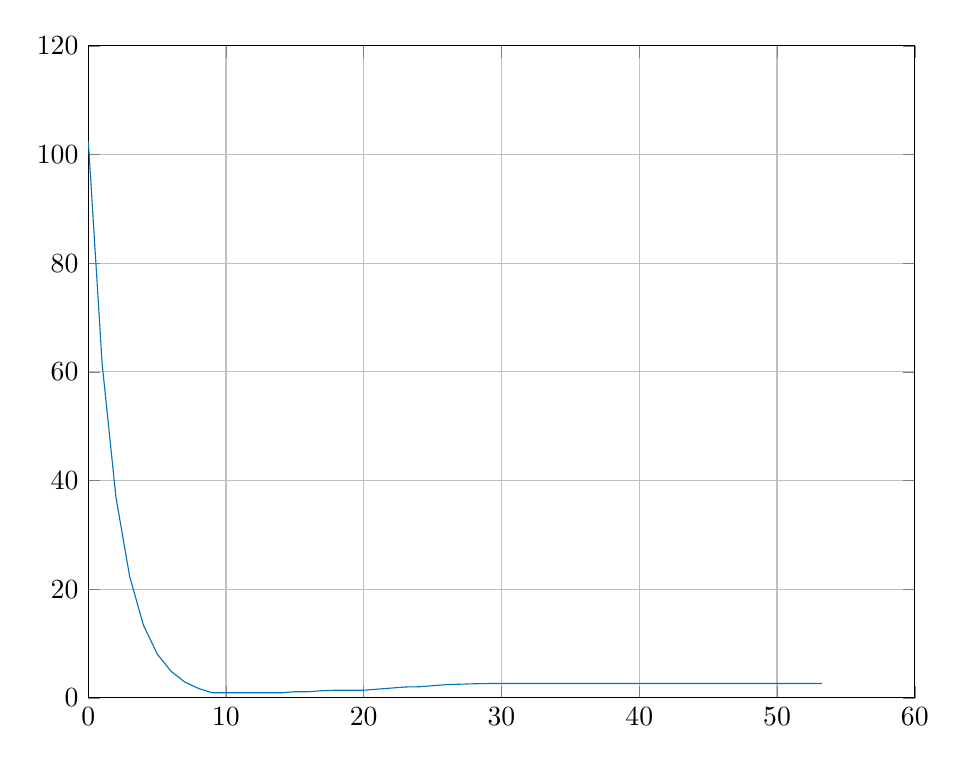
\begin{tikzpicture}

\begin{axis}[%
width=4.133in,
height=3.26in,
at={(0.693in,0.44in)},
scale only axis,
xmin=0,
xmax=60,
xmajorgrids,
ymin=0,
ymax=120,
ymajorgrids,
axis background/.style={fill=white}
]
\addplot [color=mycolor1,solid,forget plot]
  table[row sep=crcr]{%
0	102.4204\\
0.0242193229999999	101.9404\\
0.0327880259999996	101.4844\\
0.0480418650000002	100.8604\\
0.0640649849999994	100.2284\\
0.0801599199999999	99.5824\\
0.0960916940009994	98.9324\\
0.112068041	98.2684\\
0.128034914001	97.6184\\
0.144597439999999	96.9584\\
0.159984858	96.3184\\
0.175990886	95.6664\\
0.194118981	94.9924\\
0.209063808000999	94.3484\\
0.223993057001	93.6764\\
0.240054835	93.0444\\
0.256229881001	92.3924\\
0.272144378	91.7404\\
0.287973851	91.0724\\
0.304184932001	90.4264\\
0.320006189001	89.7764\\
0.336185140001	89.1344\\
0.352028416999999	88.4844\\
0.368180311	87.8324\\
0.383956049	87.1804\\
0.400114544001	86.5224\\
0.416170480001	85.8564\\
0.432047214001	85.2084\\
0.448242725	84.5604\\
0.464144897001	83.9104\\
0.479970613	83.2484\\
0.495969115	82.5804\\
0.511940392001	81.9644\\
0.528031694000999	81.3004\\
0.544822698	80.6304\\
0.560112539	79.9864\\
0.576085453	79.3384\\
0.592217994001	78.6764\\
0.608194154000999	78.0324\\
0.624183182001	77.3764\\
0.640002856	76.7304\\
0.655939531001	76.0784\\
0.67208035	75.4184\\
0.688020547	74.7664\\
0.704088285999999	74.1024\\
0.719941879	73.4544\\
0.735980507999999	72.8044\\
0.752017228	72.1564\\
0.768067579001	71.4744\\
0.784097617	70.8324\\
0.799937263	70.1544\\
0.816362714	69.4904\\
0.832030694000999	68.8604\\
0.848142964	68.2284\\
0.863985117	67.5804\\
0.880131814999999	66.9284\\
0.896147038	66.2724\\
0.912177310001	65.6144\\
0.92817121	64.9664\\
0.944042552	64.2924\\
0.960092175001	63.6384\\
0.97608091	62.9944\\
0.992225938	62.3464\\
1.008004202	61.6704\\
1.025312731	61.2024\\
1.040405422	60.8324\\
1.056007088	60.4584\\
1.071991636	60.0284\\
1.088029861	59.6524\\
1.104028046	59.2684\\
1.120102163001	58.8704\\
1.136003706001	58.4844\\
1.152097580999	58.0984\\
1.167964474	57.6964\\
1.183967715	57.3104\\
1.200080774001	56.9164\\
1.217545259	56.5124\\
1.232614123001	56.1304\\
1.248184453	55.6764\\
1.264028181	55.3384\\
1.280088982001	54.9504\\
1.296307652	54.5624\\
1.312070889	54.1704\\
1.328134628	53.7764\\
1.344152047	53.3704\\
1.360217355001	52.9664\\
1.375942069001	52.5884\\
1.392155457	52.1984\\
1.40803931	51.8104\\
1.424063084999	51.4204\\
1.440043269	51.0264\\
1.456055635001	50.6304\\
1.472141833	50.2304\\
1.488113141	49.8324\\
1.503937033	49.4464\\
1.521963832	49.0404\\
1.536079907	48.6644\\
1.552387264	48.2484\\
1.568043747	47.8524\\
1.584246563	47.4644\\
1.599971151	47.0764\\
1.618418601	46.6804\\
1.63382281	46.2884\\
1.649339064001	45.8824\\
1.664357389	45.5024\\
1.680180611	45.1164\\
1.695932958001	44.7324\\
1.714218380001	44.3224\\
1.728156815	43.9384\\
1.744040319001	43.5384\\
1.759989224	43.1524\\
1.776122056	42.7644\\
1.792076019	42.3704\\
1.808093763	41.9824\\
1.824108307001	41.5844\\
1.840630014	41.1844\\
1.856094765001	40.7884\\
1.872284567	40.4004\\
1.888195899001	40.0144\\
1.904963763001	39.6104\\
1.920297617	39.2224\\
1.936179352	38.8304\\
1.964839913001	38.3784\\
1.967988437001	38.0504\\
1.983955525	37.6384\\
1.999996847001	37.2524\\
2.017272024001	36.8844\\
2.03223906	36.6704\\
2.048014026	36.4504\\
2.063981401	36.2144\\
2.079965743	35.9724\\
2.095988529001	35.7444\\
2.114244725	35.4984\\
2.129356896	35.2604\\
2.144548017001	35.0344\\
2.16136419	34.7984\\
2.176531397	34.5604\\
2.192018813001	34.3364\\
2.208005749	34.1044\\
2.226098818	33.8664\\
2.241103213001	33.6324\\
2.256037311	33.3964\\
2.272160726	33.1604\\
2.288221274001	32.9284\\
2.303966119001	32.6904\\
2.320089134	32.4584\\
2.336055611	32.2244\\
2.352127380001	31.9944\\
2.367950083001	31.7604\\
2.384032437001	31.5184\\
2.399976935	31.2844\\
2.416037682	31.0544\\
2.432060473	30.8164\\
2.448176772001	30.5864\\
2.464228577	30.3524\\
2.479934563	30.1204\\
2.495996006	29.8844\\
2.512140078	29.6484\\
2.52806491	29.4144\\
2.544496462	29.1684\\
2.560049058	28.9384\\
2.576057483	28.6944\\
2.592026359001	28.4684\\
2.608186209999	28.2384\\
2.623982241001	27.9904\\
2.640017219	27.7624\\
2.656140236	27.5344\\
2.672166449001	27.2864\\
2.688019545	27.0524\\
2.704138397	26.8244\\
2.720177929	26.5844\\
2.736076105	26.3524\\
2.752188455999	26.1224\\
2.768116030001	25.8704\\
2.784108276	25.6464\\
2.800004342	25.4164\\
2.815932539001	25.1804\\
2.832104335	24.9484\\
2.848102005001	24.7204\\
2.864152909	24.4904\\
2.880082145	24.2544\\
2.895939214	24.0164\\
2.911969829001	23.7844\\
2.928074129	23.5044\\
2.943969133	23.3004\\
2.960009075	23.0684\\
2.976306353	22.8384\\
2.992822308	22.6044\\
3.008070471001	22.3544\\
3.025813761001	22.1964\\
3.040765101	22.0644\\
3.055987587	21.9204\\
3.072009315	21.7764\\
3.08794124	21.6364\\
3.103948296	21.4944\\
3.12003592	21.3484\\
3.136091608	21.2084\\
3.152140732001	21.0584\\
3.168009732001	20.9184\\
3.184184553001	20.7764\\
3.200147159	20.6344\\
3.216146684	20.4904\\
3.232130794	20.3444\\
3.248358541	20.2004\\
3.264124845	20.0524\\
3.279985112001	19.9144\\
3.295988994	19.7704\\
3.312053246001	19.6324\\
3.328218841	19.4884\\
3.345736217	19.3384\\
3.360894574001	19.1964\\
3.375997288001	19.0504\\
3.392050046001	18.9104\\
3.408014515001	18.7704\\
3.426093962	18.6244\\
3.4411845	18.4804\\
3.456179963	18.3404\\
3.472114004	18.1964\\
3.488084337	18.0564\\
3.504120185	17.9104\\
3.520133525	17.7684\\
3.535948998	17.6224\\
3.554407760001	17.4684\\
3.56945295	17.3284\\
3.584632203	17.1904\\
3.599932488999	17.0444\\
3.615948045	16.9004\\
3.632009889	16.7564\\
3.648157656	16.6224\\
3.663972159	16.4744\\
3.680133122	16.3364\\
3.69608654	16.1884\\
3.712140592	16.0464\\
3.728157392	15.9064\\
3.744146521	15.7604\\
3.760009302	15.6204\\
3.776169079	15.4764\\
3.792042076	15.3304\\
3.808028693	15.1844\\
3.824025299	15.0364\\
3.840101321001	14.8964\\
3.856251257	14.7564\\
3.872075392001	14.6164\\
3.888126839	14.4724\\
3.903974961	14.3244\\
3.92222766	14.1804\\
3.937173748001	14.0364\\
3.952233996001	13.8924\\
3.968188026	13.7524\\
3.984069800001	13.6104\\
4.000049255001	13.4684\\
4.017398266001	13.3264\\
4.032375012	13.2504\\
4.047986961001	13.1684\\
4.066180639	13.0844\\
4.081182581001	13.0004\\
4.096243165	12.9144\\
4.112103387	12.8324\\
4.128039551	12.7444\\
4.143975359001	12.6624\\
4.160031741001	12.5784\\
4.176169344	12.4904\\
4.192110735	12.4064\\
4.208178800001	12.3184\\
4.224204814001	12.2364\\
4.240128754	12.1524\\
4.256063652	12.0664\\
4.272128090001	11.9804\\
4.288133674	11.8964\\
4.303983880001	11.8124\\
4.319998057001	11.7284\\
4.336076801001	11.6424\\
4.351944126002	11.5584\\
4.368148482001	11.4744\\
4.383950485	11.3864\\
4.402286153	11.2944\\
4.417672832001	11.2144\\
4.433016479	11.1284\\
4.448285801	11.0444\\
4.464179549	10.9604\\
4.480252109001	10.8784\\
4.495997584	10.7904\\
4.511947352001	10.7044\\
4.528002541	10.6204\\
4.546167283	10.5364\\
4.561227386	10.4504\\
4.576224021	10.3644\\
4.592089817002	10.2784\\
4.610594928	10.1924\\
4.625732485	10.1084\\
4.640847443	10.0264\\
4.655993830999	9.94239999999999\\
4.671989379	9.85639999999998\\
4.688007721001	9.7744\\
4.704001346	9.68640000000001\\
4.720111343	9.60239999999999\\
4.735977558001	9.5184\\
4.752023048001	9.4344\\
4.768012026	9.34639999999999\\
4.783958059	9.2624\\
4.80017967	9.1764\\
4.816012859001	9.0904\\
4.834229718001	9.00239999999999\\
4.849594237	8.91840000000001\\
4.864814883	8.8364\\
4.880189755001	8.75239999999999\\
4.896030430001	8.66839999999999\\
4.91210311	8.58239999999999\\
4.928027444001	8.49839999999999\\
4.944057883	8.41439999999999\\
4.9599951	8.3304\\
4.976133217	8.24039999999999\\
4.992042722001	8.15639999999999\\
5.008377367	8.07239999999999\\
5.025871572	8.01239999999999\\
5.040897235	7.9624\\
5.056369201	7.91240000000001\\
5.072025723	7.86439999999999\\
5.088129793	7.8124\\
5.104118511001	7.76039999999999\\
5.120070348	7.71040000000001\\
5.136116520001	7.66040000000001\\
5.151981043	7.6104\\
5.16807909	7.56039999999999\\
5.183959685001	7.50639999999999\\
5.199987431	7.45639999999999\\
5.216091596	7.40639999999999\\
5.232245867	7.35639999999999\\
5.24802183	7.3044\\
5.264044893	7.25239999999999\\
5.280100131	7.20439999999999\\
5.295974344	7.15239999999999\\
5.312030742	7.1024\\
5.328166825	7.05239999999999\\
5.344154981	7.00239999999999\\
5.360129315	6.94839999999999\\
5.376158805	6.89439999999999\\
5.392220851	6.84439999999999\\
5.408112	6.79639999999999\\
5.424020010001	6.74639999999998\\
5.440159906001	6.69839999999999\\
5.455998922	6.6484\\
5.472162513001	6.5964\\
5.48811767	6.5444\\
5.506589709001	6.49039999999999\\
5.521793475	6.44039999999998\\
5.536897816	6.38839999999999\\
5.552087907	6.33839999999998\\
5.567982580999	6.29040000000001\\
5.584007999	6.24039999999999\\
5.599944057001	6.1844\\
5.618259642001	6.13239999999999\\
5.633213998001	6.08639999999998\\
5.648260994	6.0364\\
5.663943547999	5.98639999999999\\
5.679938264	5.93639999999999\\
5.696024449001	5.8844\\
5.712002998001	5.83439999999999\\
5.728029817002	5.78239999999998\\
5.746186855	5.72839999999999\\
5.761185727001	5.6784\\
5.776381639	5.6284\\
5.792183551	5.58239999999998\\
5.807945662001	5.53039999999999\\
5.824070017	5.47839999999999\\
5.840148122001	5.4284\\
5.856029749	5.3784\\
5.872297564001	5.3244\\
5.888064941	5.27439999999999\\
5.904166288	5.22240000000001\\
5.919956635001	5.17439999999999\\
5.93609956	5.12439999999999\\
5.951984623001	5.07239999999999\\
5.968234936	5.02239999999999\\
5.983993852	4.97240000000001\\
6.000131916	4.9224\\
6.018318086	4.87039999999999\\
6.033356140001	4.84039999999997\\
6.048353266	4.81039999999999\\
6.064007653	4.77839999999999\\
6.079992377	4.74639999999999\\
6.098394674	4.7144\\
6.113639762	4.6844\\
6.12870765	4.65239999999999\\
6.144146036	4.61839999999999\\
6.160138876	4.58839999999998\\
6.176101696	4.55839999999999\\
6.192086789	4.52839999999999\\
6.208047441	4.49639999999999\\
6.224089733	4.4644\\
6.240068371	4.4344\\
6.256013857001	4.3984\\
6.272047186	4.36639999999998\\
6.288244477001	4.33439999999999\\
6.304167205	4.3044\\
6.319963623001	4.27439999999999\\
6.336079641	4.24039999999999\\
6.351997536001	4.20839999999998\\
6.368133518	4.1784\\
6.384008026	4.14639999999999\\
6.400179644	4.11439999999999\\
6.416126643	4.08439999999999\\
6.432079229	4.0504\\
6.448246756	4.0184\\
6.464241578	3.98839999999998\\
6.480413036001	3.95839999999998\\
6.495940861	3.92440000000001\\
6.512086259	3.89439999999999\\
6.528156027001	3.8604\\
6.543987879	3.82839999999999\\
6.559948349	3.79839999999999\\
6.578379594	3.7664\\
6.593639263	3.7324\\
6.608877695	3.70239999999998\\
6.624075862001	3.66839999999999\\
6.64038065	3.63839999999999\\
6.656047742001	3.60839999999999\\
6.672145098	3.57639999999999\\
6.687976909	3.5444\\
6.704118946001	3.51439999999999\\
6.719938074001	3.47839999999999\\
6.736150930001	3.44839999999999\\
6.752026622	3.41839999999999\\
6.768033002	3.3844\\
6.784116211001	3.3544\\
6.8001296	3.32239999999999\\
6.816100019	3.2884\\
6.832236279001	3.25839999999999\\
6.848125361	3.22839999999999\\
6.863972129	3.19439999999999\\
6.879996877	3.1644\\
6.896089228	3.1344\\
6.911983934	3.0984\\
6.927959741001	3.06839999999998\\
6.94617294	3.03440000000001\\
6.961229744001	3.00239999999999\\
6.976469218001	2.97240000000001\\
6.992120195	2.93839999999999\\
7.008151694	2.9084\\
7.02398377	2.8844\\
7.040029845001	2.86839999999999\\
7.056000545	2.8484\\
7.072065796	2.82839999999999\\
7.090446934	2.8124\\
7.105593056	2.7924\\
7.120603275001	2.77439999999999\\
7.136242773	2.7544\\
7.152051005001	2.73439999999999\\
7.167945883	2.7144\\
7.184023931	2.6944\\
7.200108263	2.6764\\
7.216142829	2.66040000000001\\
7.232353449001	2.63839999999999\\
7.247991174	2.6224\\
7.264158891	2.6044\\
7.280132779	2.58439999999999\\
7.295991316	2.56439999999999\\
7.312114332	2.5444\\
7.328233381	2.52439999999999\\
7.343961576001	2.5044\\
7.359998103	2.48439999999999\\
7.376203555001	2.4684\\
7.392178186	2.45039999999999\\
7.408044287	2.43039999999999\\
7.424097862	2.4144\\
7.440048802	2.39439999999999\\
7.456183867001	2.37439999999999\\
7.472113867	2.3544\\
7.48816896	2.33439999999999\\
7.503979156001	2.31439999999999\\
7.522242752	2.29639999999999\\
7.537220709999	2.2764\\
7.552275065001	2.26039999999999\\
7.568147165	2.24239999999999\\
7.584056301001	2.2244\\
7.599943754	2.20239999999998\\
7.616133683	2.1844\\
7.631988162	2.1644\\
7.648137032001	2.14439999999999\\
7.664126491001	2.12439999999999\\
7.680052562	2.1044\\
7.696150713	2.08839999999998\\
7.711960284	2.07039999999999\\
7.728080640001	2.0504\\
7.744142049	2.03440000000001\\
7.76026695	2.01439999999999\\
7.776176586001	1.99439999999998\\
7.792020894	1.9744\\
7.808012328	1.95439999999999\\
7.824049616001	1.9344\\
7.840496445	1.9144\\
7.856109738	1.89639999999999\\
7.87203757	1.88039999999999\\
7.887960227001	1.8604\\
7.906212786001	1.83839999999998\\
7.921271095001	1.82239999999999\\
7.936467486	1.80240000000001\\
7.952141436	1.78440000000001\\
7.967977086	1.76439999999999\\
7.98597669	1.74439999999998\\
8.001245273	1.7244\\
8.015956669	1.70839999999998\\
8.032004104	1.6944\\
8.048002003	1.6844\\
8.064022365	1.67240000000001\\
8.080034065	1.65639999999999\\
8.096023069001	1.64439999999999\\
8.112136712	1.6344\\
8.128352281	1.6224\\
8.144021433	1.60839999999999\\
8.160142428001	1.59439999999999\\
8.176352369001	1.58439999999999\\
8.192129395	1.5684\\
8.208183596001	1.5564\\
8.224142155	1.5444\\
8.240005179	1.53240000000001\\
8.256085163001	1.52039999999998\\
8.272144075	1.5044\\
8.288005384	1.49439999999998\\
8.304127549	1.48439999999999\\
8.320120847	1.4684\\
8.336153445	1.45439999999999\\
8.352070757	1.4444\\
8.368029336	1.4324\\
8.384145867999	1.41840000000001\\
8.400101847001	1.40439999999998\\
8.416281241001	1.39239999999998\\
8.433839357001	1.38039999999999\\
8.449106754	1.36639999999998\\
8.464933705999	1.3544\\
8.480225233	1.34439999999999\\
8.496160021	1.32839999999999\\
8.512105988	1.31439999999999\\
8.528076531001	1.3044\\
8.544483406	1.2924\\
8.559944413001	1.27839999999999\\
8.575951833001	1.26439999999999\\
8.594016591001	1.2544\\
8.609094090001	1.24039999999999\\
8.624354928001	1.22839999999999\\
8.640018627	1.2144\\
8.656131047	1.20239999999998\\
8.672135225	1.1904\\
8.687948635001	1.17440000000001\\
8.704144187001	1.1644\\
8.720103212	1.15439999999998\\
8.735955581001	1.13839999999999\\
8.752143604	1.12439999999999\\
8.768113341001	1.11439999999999\\
8.783973758	1.1044\\
8.800145913	1.08839999999998\\
8.816161029001	1.0744\\
8.832135579	1.06439999999999\\
8.847973879	1.0504\\
8.864034371001	1.0364\\
8.880147692002	1.02439999999999\\
8.896139672	1.01439999999999\\
8.912273214	1.0004\\
8.928056655	0.984399999999994\\
8.943948794001	0.974400000000003\\
8.959934707	0.964399999999998\\
8.976052442002	0.946399999999997\\
8.992115513001	0.934399999999997\\
9.008126095	0.926400000000001\\
9.025645377	0.92240000000001\\
9.040697297	0.92240000000001\\
9.055981543001	0.92240000000001\\
9.072038907	0.92240000000001\\
9.088053347	0.92240000000001\\
9.104159	0.92240000000001\\
9.120118627	0.92240000000001\\
9.135967518	0.92240000000001\\
9.151940535	0.92240000000001\\
9.168120071	0.92240000000001\\
9.184071087	0.92240000000001\\
9.19997951	0.92240000000001\\
9.216037005001	0.92240000000001\\
9.232049947001	0.92240000000001\\
9.248015556	0.92240000000001\\
9.264111428	0.92240000000001\\
9.279998915	0.92240000000001\\
9.296029788	0.92240000000001\\
9.31202645	0.92240000000001\\
9.328120786	0.92240000000001\\
9.344071883	0.92240000000001\\
9.360123169	0.92240000000001\\
9.376208239001	0.92240000000001\\
9.392302187001	0.92240000000001\\
9.408246258	0.92240000000001\\
9.424107162	0.92240000000001\\
9.44007336	0.92240000000001\\
9.456048436	0.92240000000001\\
9.472026345	0.92240000000001\\
9.487942246001	0.92240000000001\\
9.504031882	0.92240000000001\\
9.520032236	0.92240000000001\\
9.536114986	0.92240000000001\\
9.552075666	0.92240000000001\\
9.568036654	0.92240000000001\\
9.584360098001	0.92240000000001\\
9.600309384	0.92240000000001\\
9.616469533	0.92240000000001\\
9.632015393	0.92240000000001\\
9.648171018	0.92240000000001\\
9.663934795	0.92240000000001\\
9.680156833001	0.92240000000001\\
9.696258581001	0.92240000000001\\
9.712093	0.92240000000001\\
9.728093223001	0.92240000000001\\
9.743962741001	0.92240000000001\\
9.760010072	0.92240000000001\\
9.776023395	0.92240000000001\\
9.792229922	0.92240000000001\\
9.807994181	0.92240000000001\\
9.824173416	0.92240000000001\\
9.840074708001	0.92240000000001\\
9.856001623001	0.92240000000001\\
9.872122086001	0.92240000000001\\
9.888034573	0.92240000000001\\
9.90398918	0.92240000000001\\
9.920109090001	0.92240000000001\\
9.936005028	0.92240000000001\\
9.95413703	0.92240000000001\\
9.969233226	0.92240000000001\\
9.98454429	0.92240000000001\\
9.999939262	0.92240000000001\\
10.017057415	0.92240000000001\\
10.031967953	0.92240000000001\\
10.047990769	0.92240000000001\\
10.066063698	0.92240000000001\\
10.080927415	0.92240000000001\\
10.095953801	0.92240000000001\\
10.111978234	0.92240000000001\\
10.128033653	0.92240000000001\\
10.144058868	0.92240000000001\\
10.160205388001	0.92240000000001\\
10.176156275001	0.92240000000001\\
10.192147886	0.92240000000001\\
10.208148821001	0.92240000000001\\
10.224286382	0.92240000000001\\
10.240111092	0.92240000000001\\
10.25599012	0.92240000000001\\
10.27211066	0.92240000000001\\
10.288017518001	0.92240000000001\\
10.304185502	0.92240000000001\\
10.319924344	0.92240000000001\\
10.336025222	0.92240000000001\\
10.352183596	0.92240000000001\\
10.368152383	0.92240000000001\\
10.383992147001	0.92240000000001\\
10.402205583	0.92240000000001\\
10.417306845	0.92240000000001\\
10.433035999	0.92240000000001\\
10.448037939001	0.92240000000001\\
10.464149252	0.92240000000001\\
10.479962611	0.92240000000001\\
10.498300228	0.92240000000001\\
10.513429196001	0.92240000000001\\
10.528692827001	0.92240000000001\\
10.543935436	0.92240000000001\\
10.560101652	0.92240000000001\\
10.576784553	0.92240000000001\\
10.592198801	0.92240000000001\\
10.607964462	0.92240000000001\\
10.624294415	0.92240000000001\\
10.640300958001	0.92240000000001\\
10.655991334001	0.92240000000001\\
10.67212275	0.92240000000001\\
10.687989456001	0.92240000000001\\
10.706157037	0.92240000000001\\
10.721354897001	0.92240000000001\\
10.736531721	0.92240000000001\\
10.752099264	0.92240000000001\\
10.768065312001	0.92240000000001\\
10.783980066	0.92240000000001\\
10.80003904	0.92240000000001\\
10.816115766	0.92240000000001\\
10.831949359001	0.92240000000001\\
10.847983392	0.92240000000001\\
10.865218633	0.92240000000001\\
10.880254789	0.92240000000001\\
10.895947099	0.92240000000001\\
10.914040636	0.92240000000001\\
10.929035427	0.92240000000001\\
10.944216478	0.92240000000001\\
10.959962383	0.92240000000001\\
10.976128954	0.92240000000001\\
10.992059306	0.92240000000001\\
11.008250883	0.92240000000001\\
11.025734802	0.92240000000001\\
11.04071912	0.92240000000001\\
11.056010495	0.92240000000001\\
11.072039352001	0.92240000000001\\
11.088010655	0.92240000000001\\
11.104045948	0.92240000000001\\
11.120219544	0.92240000000001\\
11.135983231	0.92240000000001\\
11.152102222001	0.92240000000001\\
11.168179173001	0.92240000000001\\
11.183985523	0.92240000000001\\
11.200006968001	0.92240000000001\\
11.216112325	0.92240000000001\\
11.232085802	0.92240000000001\\
11.248168095001	0.92240000000001\\
11.263997837	0.92240000000001\\
11.280033331001	0.92240000000001\\
11.296468391	0.92240000000001\\
11.311976059	0.92240000000001\\
11.328110871001	0.92240000000001\\
11.343956079	0.92240000000001\\
11.360097774001	0.92240000000001\\
11.376043861	0.92240000000001\\
11.391960171	0.92240000000001\\
11.410109705	0.92240000000001\\
11.425170172999	0.92240000000001\\
11.440386045	0.92240000000001\\
11.4562105	0.92240000000001\\
11.472076883	0.92240000000001\\
11.488033929	0.92240000000001\\
11.504026493	0.92240000000001\\
11.520049507	0.92240000000001\\
11.536151308001	0.92240000000001\\
11.552010416	0.92240000000001\\
11.568117153	0.92240000000001\\
11.583989422	0.92240000000001\\
11.599973419	0.92240000000001\\
11.615933086	0.92240000000001\\
11.632621853	0.92240000000001\\
11.647967852	0.92240000000001\\
11.664097634	0.92240000000001\\
11.67993604	0.92240000000001\\
11.69813573	0.92240000000001\\
11.711976038001	0.92240000000001\\
11.728183045	0.92240000000001\\
11.743959744001	0.92240000000001\\
11.760214326	0.92240000000001\\
11.776205091	0.92240000000001\\
11.792109383	0.92240000000001\\
11.80799667	0.92240000000001\\
11.824439302	0.92240000000001\\
11.839932576	0.92240000000001\\
11.858086580999	0.92240000000001\\
11.873153165	0.92240000000001\\
11.888163571001	0.92240000000001\\
11.904050503001	0.92240000000001\\
11.920017878	0.92240000000001\\
11.936164057001	0.92240000000001\\
11.952099602	0.92240000000001\\
11.968164585	0.92240000000001\\
11.984203697	0.92240000000001\\
12.000454289	0.92240000000001\\
12.015927390001	0.92240000000001\\
12.031984746001	0.92240000000001\\
12.048006594	0.92240000000001\\
12.063973254	0.92240000000001\\
12.082115007	0.92240000000001\\
12.097085428	0.92240000000001\\
12.112062613999	0.92240000000001\\
12.128142163001	0.92240000000001\\
12.144166917001	0.92240000000001\\
12.160007267001	0.92240000000001\\
12.176034996001	0.92240000000001\\
12.192049981	0.92240000000001\\
12.208046473001	0.92240000000001\\
12.224081666	0.92240000000001\\
12.23995687	0.92240000000001\\
12.256108640001	0.92240000000001\\
12.27216716	0.92240000000001\\
12.287978376	0.92240000000001\\
12.304103017001	0.92240000000001\\
12.320039877	0.92240000000001\\
12.335930723	0.92240000000001\\
12.352171823	0.92240000000001\\
12.368068452	0.92240000000001\\
12.383916506001	0.92240000000001\\
12.400022615	0.92240000000001\\
12.416032531001	0.92240000000001\\
12.432261967	0.92240000000001\\
12.448231158	0.92240000000001\\
12.464263895	0.92240000000001\\
12.480264731	0.92240000000001\\
12.496091777	0.92240000000001\\
12.512209507	0.92240000000001\\
12.52827317	0.92240000000001\\
12.544169629	0.92240000000001\\
12.560101307	0.92240000000001\\
12.576085555001	0.92240000000001\\
12.592170576	0.92240000000001\\
12.60809241	0.92240000000001\\
12.624037584001	0.92240000000001\\
12.639961197	0.92240000000001\\
12.658097632	0.92240000000001\\
12.67309724	0.92240000000001\\
12.688153742	0.92240000000001\\
12.704039701001	0.92240000000001\\
12.719958340001	0.92240000000001\\
12.736117774001	0.92240000000001\\
12.752169557001	0.92240000000001\\
12.76821099	0.92240000000001\\
12.784076719	0.92240000000001\\
12.800080716001	0.92240000000001\\
12.816059884	0.92240000000001\\
12.832087063	0.92240000000001\\
12.848206246001	0.92240000000001\\
12.863950218	0.92240000000001\\
12.880152963	0.92240000000001\\
12.896052338	0.92240000000001\\
12.911911772	0.92240000000001\\
12.928090075	0.92240000000001\\
12.944187799	0.92240000000001\\
12.959948769	0.92240000000001\\
12.976028751002	0.92240000000001\\
12.994426068	0.92240000000001\\
13.009745178	0.92240000000001\\
13.024175590001	0.92240000000001\\
13.040213328	0.92240000000001\\
13.055951561	0.92240000000001\\
13.074444046	0.92240000000001\\
13.089596844	0.92240000000001\\
13.104860473	0.92240000000001\\
13.120156712	0.92240000000001\\
13.13608849	0.92240000000001\\
13.151942964	0.92240000000001\\
13.168095222001	0.92240000000001\\
13.184057716	0.92240000000001\\
13.199934257	0.92240000000001\\
13.216060589	0.92240000000001\\
13.232170968	0.92240000000001\\
13.248052927	0.92240000000001\\
13.264085872	0.92240000000001\\
13.280123911001	0.92240000000001\\
13.295951639	0.92240000000001\\
13.312201318	0.92240000000001\\
13.328197232001	0.92240000000001\\
13.344180091999	0.92240000000001\\
13.360199444001	0.92240000000001\\
13.376219829001	0.92240000000001\\
13.392372232001	0.92240000000001\\
13.408071469	0.92240000000001\\
13.424192402001	0.92240000000001\\
13.440036822	0.92240000000001\\
13.456220983	0.92240000000001\\
13.472228459001	0.92240000000001\\
13.488190431	0.92240000000001\\
13.504227157	0.92240000000001\\
13.520193053	0.92240000000001\\
13.535934697	0.92240000000001\\
13.552053895	0.92240000000001\\
13.568067363999	0.92240000000001\\
13.584047189001	0.92240000000001\\
13.600395509	0.92240000000001\\
13.616075142001	0.92240000000001\\
13.631935496001	0.92240000000001\\
13.648055218	0.92240000000001\\
13.66409403	0.92240000000001\\
13.680007220001	0.92240000000001\\
13.696180061	0.92240000000001\\
13.712153354	0.92240000000001\\
13.728193644	0.92240000000001\\
13.744197020001	0.92240000000001\\
13.760054085	0.92240000000001\\
13.775972422999	0.92240000000001\\
13.792221856	0.92240000000001\\
13.808213486	0.92240000000001\\
13.824223988	0.92240000000001\\
13.840444882	0.92240000000001\\
13.85617998	0.92240000000001\\
13.871956239001	0.92240000000001\\
13.888058502	0.92240000000001\\
13.904060209	0.92240000000001\\
13.920045339	0.92240000000001\\
13.93602924	0.92240000000001\\
13.952193516	0.92240000000001\\
13.968219383	0.92240000000001\\
13.984314663	0.92240000000001\\
14.000287815001	0.92240000000001\\
14.017872815999	0.92240000000001\\
14.032853885001	0.928399999999996\\
14.04813085	0.928399999999996\\
14.063920759	0.932400000000001\\
14.079968812001	0.936399999999992\\
14.09597494	0.938399999999987\\
14.112024616001	0.942399999999992\\
14.127951902	0.946399999999997\\
14.146103173001	0.948399999999992\\
14.161112888999	0.950399999999988\\
14.176229618	0.956399999999988\\
14.192061681	0.958399999999983\\
14.208004349	0.960399999999979\\
14.224048692	0.962399999999988\\
14.240114865	0.968400000000003\\
14.25604446	0.968400000000003\\
14.272018853	0.972399999999993\\
14.288265748001	0.978399999999993\\
14.304047795	0.978399999999993\\
14.319993158	0.982399999999998\\
14.335991425001	0.988399999999984\\
14.352051938	0.988399999999984\\
14.368026875	0.992399999999989\\
14.383964693	0.99839999999999\\
14.400005164001	0.99839999999999\\
14.41598425	1.00239999999999\\
14.431949561	1.0064\\
14.447992672999	1.00839999999999\\
14.46396212	1.01039999999999\\
14.479953551	1.01639999999999\\
14.497960065	1.01839999999999\\
14.513061199001	1.02039999999998\\
14.528015916	1.02239999999999\\
14.543937678001	1.02839999999999\\
14.559920981	1.03040000000001\\
14.575984129	1.03240000000001\\
14.591964991001	1.0384\\
14.607987754	1.0384\\
14.623959416	1.0424\\
14.639936519	1.0484\\
14.658048359001	1.0484\\
14.672995384	1.05240000000001\\
14.688022972	1.05839999999999\\
14.703978705999	1.05839999999999\\
14.719960278	1.0624\\
14.735969719	1.0664\\
14.751963929	1.0684\\
14.767985574001	1.07239999999999\\
14.783971766	1.07639999999999\\
14.800000965001	1.07839999999999\\
14.816003208001	1.08039999999998\\
14.83197424	1.08439999999999\\
14.847947046001	1.08839999999998\\
14.865997977	1.0904\\
14.880876079001	1.0924\\
14.895945914001	1.0984\\
14.914010545	1.0984\\
14.928956639	1.10239999999999\\
14.944096313	1.10839999999999\\
14.959940052	1.10839999999999\\
14.977998419	1.11239999999999\\
14.99248885	1.11839999999999\\
15.007947591001	1.11839999999999\\
15.025125496001	1.11839999999999\\
15.040239733	1.11839999999999\\
15.056002728001	1.11839999999999\\
15.072093026	1.11839999999999\\
15.088043972001	1.11839999999999\\
15.104046882	1.11839999999999\\
15.120115881	1.11839999999999\\
15.135965094	1.11839999999999\\
15.151944926999	1.11839999999999\\
15.167959363	1.11839999999999\\
15.183956314001	1.11839999999999\\
15.200001934	1.11839999999999\\
15.216044125	1.11839999999999\\
15.231981276	1.11839999999999\\
15.248022293001	1.11839999999999\\
15.265388255001	1.11839999999999\\
15.280510863	1.11839999999999\\
15.296103307001	1.11839999999999\\
15.312025048001	1.11839999999999\\
15.328226112	1.11839999999999\\
15.344125686	1.11839999999999\\
15.360032655	1.11839999999999\\
15.376051917	1.11839999999999\\
15.392168182001	1.11839999999999\\
15.408146024001	1.11839999999999\\
15.424050384	1.11839999999999\\
15.44013092	1.11839999999999\\
15.456084678001	1.11839999999999\\
15.472008637	1.11839999999999\\
15.488017699001	1.11839999999999\\
15.504011342	1.11839999999999\\
15.520187575	1.11839999999999\\
15.536038665	1.11839999999999\\
15.552057346001	1.11839999999999\\
15.568156134	1.11839999999999\\
15.584110313	1.11839999999999\\
15.599955122	1.11839999999999\\
15.616035925001	1.11839999999999\\
15.63193753	1.11839999999999\\
15.648395200001	1.11839999999999\\
15.664141529001	1.11839999999999\\
15.680121996001	1.11839999999999\\
15.696186225	1.11839999999999\\
15.712050262	1.11839999999999\\
15.727969455	1.11839999999999\\
15.743956968	1.11839999999999\\
15.759970263	1.11839999999999\\
15.775963121	1.11839999999999\\
15.791941925	1.11839999999999\\
15.810058381	1.11839999999999\\
15.824964641	1.11839999999999\\
15.840025344	1.11839999999999\\
15.858192539	1.11839999999999\\
15.873213751002	1.11839999999999\\
15.888055493	1.11839999999999\\
15.903934448	1.11839999999999\\
15.922047077	1.11839999999999\\
15.936959092	1.11839999999999\\
15.951953902	1.11839999999999\\
15.967968604	1.11839999999999\\
15.986021198	1.11839999999999\\
16.000943049	1.11839999999999\\
16.01594028	1.12039999999999\\
16.032021153	1.12439999999999\\
16.048109767	1.12839999999998\\
16.063930708	1.12839999999998\\
16.082000668001	1.13239999999999\\
16.096892569001	1.13839999999999\\
16.111950638	1.13839999999999\\
16.13003492	1.14239999999998\\
16.145890872	1.14839999999998\\
16.16082807	1.14839999999998\\
16.175941745	1.15239999999999\\
16.194018714001	1.15639999999999\\
16.2090256	1.1584\\
16.224440495	1.16240000000001\\
16.240345434	1.1664\\
16.255977984001	1.16840000000001\\
16.271989916	1.17240000000001\\
16.28798696	1.1764\\
16.306113251	1.1784\\
16.321630018	1.1824\\
16.337183805001	1.18639999999999\\
16.352247915	1.18839999999999\\
16.368033457	1.18839999999999\\
16.384241726	1.19239999999999\\
16.399962451001	1.19839999999999\\
16.416033837	1.19839999999999\\
16.431991984	1.20239999999998\\
16.447966508	1.20839999999998\\
16.463948317	1.20839999999998\\
16.482016895	1.21239999999999\\
16.497216369	1.2184\\
16.512145205	1.2184\\
16.527933763	1.22239999999999\\
16.546039057001	1.2264\\
16.560871493	1.22839999999999\\
16.575940468	1.2324\\
16.592056942002	1.23639999999999\\
16.607932464	1.23839999999998\\
16.623975382	1.24039999999999\\
16.640002459	1.24639999999999\\
16.656442683	1.24839999999999\\
16.672016509	1.25039999999998\\
16.687994806	1.2544\\
16.703971532001	1.25839999999999\\
16.7199336	1.25839999999999\\
16.7359571	1.26239999999999\\
16.754063799	1.26839999999999\\
16.769586067	1.26839999999999\\
16.784467906	1.27239999999999\\
16.799935194001	1.27839999999999\\
16.815941295	1.27839999999999\\
16.831973230001	1.28240000000001\\
16.84814942	1.2864\\
16.864186894	1.2884\\
16.879955075	1.2924\\
16.898134795	1.29639999999999\\
16.913271745	1.2984\\
16.92839445	1.30240000000001\\
16.944015853	1.3064\\
16.960084675	1.30839999999999\\
16.976356111	1.31039999999999\\
16.992000057	1.31440000000001\\
17.010421186	1.3184\\
17.0249998	1.3184\\
17.040167535	1.32039999999999\\
17.056179402001	1.32239999999999\\
17.072169032001	1.32239999999999\\
17.088009812001	1.32239999999999\\
17.104115969	1.32639999999999\\
17.120065548001	1.32639999999999\\
17.136029598	1.32639999999999\\
17.153880814001	1.33039999999998\\
17.169119697001	1.33039999999998\\
17.184214148	1.33039999999998\\
17.200302822001	1.33239999999998\\
17.216098095	1.33439999999999\\
17.232239295	1.33439999999999\\
17.248040612	1.3364\\
17.264109680001	1.33839999999999\\
17.280129361	1.33839999999999\\
17.296109214	1.34039999999999\\
17.312081525	1.34239999999998\\
17.328190385	1.34239999999998\\
17.344052714	1.34439999999999\\
17.360202699001	1.34639999999999\\
17.376166591001	1.34639999999999\\
17.392119297	1.34639999999999\\
17.408059769	1.35039999999999\\
17.423986518001	1.35039999999999\\
17.440277202	1.35039999999999\\
17.456137487	1.35439999999998\\
17.47214912	1.35439999999998\\
17.488145663	1.35439999999998\\
17.504133539001	1.35639999999998\\
17.520025115	1.35839999999999\\
17.536173806	1.35839999999999\\
17.552191059	1.3604\\
17.56800801	1.36239999999999\\
17.584166425	1.36239999999999\\
17.600082087	1.36439999999999\\
17.616021501002	1.36639999999998\\
17.632126019	1.36639999999998\\
17.648145289	1.36839999999999\\
17.664117454	1.37039999999999\\
17.680156172	1.37039999999999\\
17.696049961	1.3724\\
17.712162789	1.37439999999999\\
17.728069746	1.37439999999999\\
17.744183497	1.37439999999999\\
17.760126116001	1.37839999999998\\
17.776057076	1.37839999999998\\
17.792137403	1.37839999999998\\
17.808269843001	1.38239999999999\\
17.823994672999	1.38239999999999\\
17.840187322	1.38239999999999\\
17.856099475	1.3844\\
17.872047511	1.38639999999999\\
17.888145617	1.38639999999999\\
17.904251774	1.38839999999999\\
17.920043016	1.39039999999999\\
17.936123011001	1.39039999999999\\
17.952073832	1.39239999999999\\
17.968102601	1.39439999999999\\
17.984024625	1.39439999999999\\
18.000031024001	1.3964\\
18.017971661	1.3964\\
18.033073836001	1.3964\\
18.04844532	1.3964\\
18.064137832	1.3964\\
18.080174092	1.3964\\
18.096052164	1.3964\\
18.1122474	1.3964\\
18.12817341	1.3964\\
18.143993046	1.3964\\
18.160165735	1.3964\\
18.176084731	1.3964\\
18.192093624	1.3964\\
18.208263988	1.3964\\
18.224187814001	1.3964\\
18.240182215001	1.3964\\
18.256107038001	1.3964\\
18.274413303	1.3964\\
18.289644760001	1.3964\\
18.305149896	1.3964\\
18.320253298001	1.3964\\
18.335948349	1.3964\\
18.35209925	1.3964\\
18.370251727001	1.3964\\
18.385494349	1.3964\\
18.400658072001	1.3964\\
18.416241206001	1.3964\\
18.432043932	1.3964\\
18.448132441	1.3964\\
18.464063097001	1.3964\\
18.480098746001	1.3964\\
18.496127159	1.3964\\
18.512040518	1.3964\\
18.528212068	1.3964\\
18.544168172	1.3964\\
18.560065398	1.3964\\
18.576014127	1.3964\\
18.592111509	1.3964\\
18.608161446	1.3964\\
18.624021947	1.3964\\
18.64042308	1.3964\\
18.656176348	1.3964\\
18.672235475	1.3964\\
18.68813317	1.3964\\
18.704100341999	1.3964\\
18.720168271	1.3964\\
18.736190113	1.3964\\
18.752159216	1.3964\\
18.768091203	1.3964\\
18.784315026	1.3964\\
18.800092635001	1.3964\\
18.815998672	1.3964\\
18.832054340001	1.3964\\
18.847956105001	1.3964\\
18.864133006	1.3964\\
18.880126374001	1.3964\\
18.896135889	1.3964\\
18.911976636	1.3964\\
18.928136401	1.3964\\
18.944216732001	1.3964\\
18.960204102001	1.3964\\
18.976382058	1.3964\\
18.991996405	1.3964\\
19.008047494001	1.3964\\
19.025816234001	1.3964\\
19.04103881	1.3964\\
19.056242499	1.3964\\
19.074670581001	1.3964\\
19.089938229	1.3964\\
19.105082303	1.3964\\
19.120813354	1.3964\\
19.136173928	1.3964\\
19.152156669001	1.3964\\
19.16805836	1.3964\\
19.184086339001	1.3964\\
19.199976513	1.3964\\
19.216193838001	1.3964\\
19.232118962	1.3964\\
19.248140755001	1.3964\\
19.264195677	1.3964\\
19.280025888001	1.3964\\
19.296040738999	1.3964\\
19.312028224	1.3964\\
19.327933142001	1.3964\\
19.344160021	1.3964\\
19.360005697	1.3964\\
19.375975366001	1.3964\\
19.392199122	1.3964\\
19.407954717	1.3964\\
19.426056744001	1.3964\\
19.440888209	1.3964\\
19.455942729	1.3964\\
19.471972676	1.3964\\
19.487941889	1.3964\\
19.503996436	1.3964\\
19.519994472001	1.3964\\
19.535996826	1.3964\\
19.552112776	1.3964\\
19.567926626	1.3964\\
19.58592999	1.3964\\
19.6008152	1.3964\\
19.615994069001	1.3964\\
19.631937856	1.3964\\
19.650150138001	1.3964\\
19.665500613999	1.3964\\
19.681449232001	1.3964\\
19.696648264	1.3964\\
19.712156228	1.3964\\
19.72898402	1.3964\\
19.744349358	1.3964\\
19.760017695	1.3964\\
19.776219349	1.3964\\
19.792174782	1.3964\\
19.80809071	1.3964\\
19.824120986	1.3964\\
19.840125098	1.3964\\
19.856724681001	1.3964\\
19.872069861	1.3964\\
19.889652962	1.3964\\
19.904807109	1.3964\\
19.920039105001	1.3964\\
19.936044205	1.3964\\
19.952125654	1.3964\\
19.967969363	1.3964\\
19.983938886	1.3964\\
20.002072357001	1.3964\\
20.016998015001	1.3984\\
20.032167546	1.40239999999999\\
20.048049079001	1.40439999999998\\
20.064099757	1.40839999999999\\
20.08013691	1.41239999999998\\
20.096156615	1.41439999999997\\
20.112229932001	1.4164\\
20.12813844	1.4224\\
20.144107914	1.42439999999999\\
20.160132818	1.42639999999999\\
20.175991841001	1.43039999999999\\
20.191992091999	1.43239999999999\\
20.208032517	1.43639999999999\\
20.224021953	1.4384\\
20.242368203	1.44239999999999\\
20.257614863999	1.4464\\
20.272811683	1.44839999999999\\
20.288158289	1.4524\\
20.30404448	1.4564\\
20.320170564001	1.4584\\
20.336276527	1.46239999999999\\
20.352191328	1.46439999999998\\
20.368122982001	1.46839999999999\\
20.384307774001	1.47239999999998\\
20.400016958001	1.47439999999997\\
20.418169124	1.47839999999998\\
20.433475766	1.4824\\
20.448773197	1.48440000000001\\
20.464431536	1.4864\\
20.48017323	1.49039999999999\\
20.496085	1.4924\\
20.512147873001	1.49640000000001\\
20.527942837	1.5004\\
20.546267409002	1.50239999999999\\
20.561412365	1.5064\\
20.576556954001	1.50839999999999\\
20.592256881	1.51239999999999\\
20.608307205	1.5164\\
20.624421412	1.5184\\
20.640100741001	1.52239999999999\\
20.656145403	1.5264\\
20.672144961	1.52839999999999\\
20.688060743	1.53239999999998\\
20.704118833001	1.53439999999998\\
20.720133364001	1.53839999999998\\
20.735924228	1.5424\\
20.75213303	1.5444\\
20.768078277	1.54639999999999\\
20.784009102001	1.55239999999999\\
20.800100677	1.5544\\
20.816092015001	1.5564\\
20.832106948	1.56039999999999\\
20.848194004	1.5624\\
20.864154535	1.56639999999999\\
20.880045549	1.5684\\
20.896160411	1.57239999999999\\
20.914496486	1.57640000000001\\
20.92954596	1.5784\\
20.944734154001	1.58239999999999\\
20.960031621001	1.5864\\
20.976411758	1.58839999999999\\
20.992137722001	1.59239999999998\\
21.008200428	1.59439999999998\\
21.025954893001	1.59839999999998\\
21.041145351	1.60239999999999\\
21.056341648	1.60439999999998\\
21.071969672	1.60640000000001\\
21.090104871	1.61240000000001\\
21.105235691	1.6144\\
21.120396916	1.6164\\
21.136113026	1.62039999999999\\
21.152144076001	1.6224\\
21.167976349	1.6264\\
21.184168132	1.63039999999999\\
21.200097681	1.63239999999999\\
21.216028277	1.63639999999999\\
21.232005741001	1.63839999999999\\
21.248163419001	1.64239999999999\\
21.264119774001	1.6464\\
21.280159939001	1.6484\\
21.296090916	1.65239999999999\\
21.312018984	1.65639999999999\\
21.328086091	1.65839999999999\\
21.344058497	1.66239999999998\\
21.360114918001	1.66439999999997\\
21.376214921001	1.66839999999999\\
21.392143560001	1.6724\\
21.408443445	1.67439999999999\\
21.424181378	1.67839999999998\\
21.440290549	1.68239999999999\\
21.456106640001	1.6844\\
21.474421831001	1.68639999999999\\
21.48813735	1.6904\\
21.504006327001	1.69239999999999\\
21.520173220001	1.6964\\
21.536188287	1.69839999999999\\
21.552011004	1.7024\\
21.568110883	1.7064\\
21.584037197001	1.7084\\
21.600065758	1.71239999999999\\
21.617376257	1.71639999999999\\
21.632609076001	1.71839999999999\\
21.64812592	1.72239999999998\\
21.664116131	1.72439999999997\\
21.680011903	1.72839999999998\\
21.695997435	1.7324\\
21.712215591	1.73440000000001\\
21.728026205	1.7364\\
21.744056187001	1.7424\\
21.760103357001	1.74440000000001\\
21.776156249999	1.7484\\
21.792119952	1.7504\\
21.808230191	1.7544\\
21.824142230001	1.7564\\
21.840185576001	1.76039999999999\\
21.856079389	1.76239999999999\\
21.872106282	1.7664\\
21.888215528	1.7684\\
21.904071149001	1.77239999999999\\
21.919940047999	1.7764\\
21.936114976	1.77839999999999\\
21.952052225	1.78239999999998\\
21.968074091001	1.78639999999999\\
21.984190602	1.78839999999998\\
22.000064155	1.7924\\
22.018094888001	1.79639999999999\\
22.03329683	1.79839999999999\\
22.048449492	1.80239999999999\\
22.064404935	1.8044\\
22.08007994	1.8064\\
22.096088053	1.8124\\
22.112141664001	1.8124\\
22.128239148	1.81639999999999\\
22.144106002	1.82039999999999\\
22.160114352	1.82239999999999\\
22.176165050001	1.82640000000001\\
22.192314998001	1.8284\\
22.20829106	1.83239999999999\\
22.224146032	1.8364\\
22.240156274001	1.83839999999999\\
22.256193777001	1.84239999999998\\
22.272141227001	1.84639999999999\\
22.288011002	1.84839999999998\\
22.304197992	1.85239999999999\\
22.320099196001	1.85439999999998\\
22.336080768	1.8584\\
22.352033695	1.86240000000001\\
22.368005365	1.8644\\
22.384060445	1.8664\\
22.401769365	1.8724\\
22.417012153	1.87440000000001\\
22.432375471	1.8764\\
22.448502394	1.88039999999999\\
22.464138957	1.88239999999999\\
22.480143430001	1.88639999999999\\
22.496081854	1.89039999999999\\
22.512204842	1.89239999999999\\
22.528122774001	1.8964\\
22.544426195	1.8984\\
22.560080264	1.90239999999999\\
22.576119662	1.90639999999999\\
22.592135832	1.90839999999999\\
22.608175139	1.91239999999998\\
22.624115894	1.9164\\
22.640400552	1.91839999999999\\
22.656081427	1.9224\\
22.672164494001	1.92439999999999\\
22.688050056	1.92839999999998\\
22.7041195	1.93239999999999\\
22.720100905	1.9344\\
22.736113833001	1.93639999999999\\
22.752143504001	1.94239999999999\\
22.768044544	1.94239999999999\\
22.784132269	1.9464\\
22.800077088001	1.95039999999999\\
22.816147496001	1.9524\\
22.832093702001	1.9564\\
22.848125082	1.9584\\
22.864264461	1.96239999999999\\
22.880083492	1.96639999999999\\
22.896152174	1.96839999999999\\
22.912216262	1.97239999999998\\
22.928054089	1.97639999999998\\
22.944149923001	1.97839999999998\\
22.960113133	1.9824\\
22.976079899	1.9864\\
22.99206621	1.9884\\
23.008208871001	1.9924\\
23.025768739001	1.9924\\
23.040920797999	1.9944\\
23.056132634	1.9944\\
23.072207216001	1.9944\\
23.088149052	1.99639999999999\\
23.104031906001	1.99639999999999\\
23.120038856	1.99639999999999\\
23.136048935	1.99639999999999\\
23.152134959	1.99839999999999\\
23.168180340001	1.99839999999999\\
23.184022801	1.99839999999999\\
23.200094582	2.00039999999998\\
23.21618044	2.00039999999998\\
23.232061755001	2.00039999999998\\
23.248155718	2.00239999999999\\
23.264151699001	2.00239999999999\\
23.28000817	2.00239999999999\\
23.296098191	2.00439999999999\\
23.312150849	2.00439999999999\\
23.328037444	2.00439999999999\\
23.344167343001	2.00639999999999\\
23.360157779001	2.00639999999999\\
23.376264027001	2.00639999999999\\
23.393738899001	2.00639999999999\\
23.408877023	2.00840000000001\\
23.424142558	2.00840000000001\\
23.44257303	2.00840000000001\\
23.457752825	2.0104\\
23.472858216	2.0104\\
23.488164647	2.0104\\
23.504068064001	2.0124\\
23.519977061	2.0124\\
23.536169974	2.0124\\
23.552015782	2.01439999999999\\
23.568161722001	2.01439999999999\\
23.584170972001	2.01439999999999\\
23.599998515001	2.0164\\
23.616157469	2.0164\\
23.632168369	2.0164\\
23.648149205999	2.0184\\
23.664132735001	2.0184\\
23.680140744001	2.0184\\
23.696075971	2.0184\\
23.712135148	2.0204\\
23.728146088001	2.0204\\
23.744098988	2.0204\\
23.760130994	2.02239999999999\\
23.776094183	2.02239999999999\\
23.792105569001	2.02239999999999\\
23.808198241001	2.02439999999999\\
23.824108391	2.02439999999999\\
23.840321171	2.02439999999999\\
23.856028638001	2.0264\\
23.872117587	2.0264\\
23.888110093	2.0264\\
23.904120315	2.02839999999999\\
23.920122636	2.02839999999999\\
23.935987533	2.02839999999999\\
23.952091785	2.03039999999999\\
23.968158736	2.03039999999999\\
23.984146118	2.03039999999999\\
24.000003756	2.03240000000001\\
24.017450011	2.03240000000001\\
24.032795003001	2.0364\\
24.048203930001	2.0384\\
24.064114235	2.0424\\
24.080190832	2.04639999999999\\
24.096124901	2.04839999999999\\
24.112138039	2.05240000000001\\
24.128091567002	2.0544\\
24.144107988999	2.0564\\
24.160091185	2.06039999999999\\
24.176058922	2.06439999999999\\
24.192159844	2.06639999999999\\
24.208314595	2.07039999999999\\
24.22409925	2.0744\\
24.240369522	2.07639999999999\\
24.256066322	2.08039999999998\\
24.272110686	2.0844\\
24.288258510001	2.0864\\
24.304128985001	2.0904\\
24.32005185	2.09440000000001\\
24.336135716	2.0964\\
24.352164595001	2.0984\\
24.368136487	2.1024\\
24.384109005	2.10639999999999\\
24.400112738	2.10839999999999\\
24.416057133	2.11239999999999\\
24.432052336	2.11439999999999\\
24.448171421001	2.1164\\
24.464141412	2.1224\\
24.480039619	2.12439999999999\\
24.496083011	2.12639999999999\\
24.512240617	2.13239999999999\\
24.528120883	2.1344\\
24.544161975	2.13639999999999\\
24.560045925	2.1404\\
24.576187463001	2.14439999999999\\
24.592192599	2.1464\\
24.608112877	2.15039999999999\\
24.624149397	2.15439999999998\\
24.640230506	2.15639999999999\\
24.656085205	2.16040000000001\\
24.672172416	2.16240000000001\\
24.688112363	2.1664\\
24.704095172	2.16839999999999\\
24.720174876002	2.1724\\
24.736147738	2.1764\\
24.752103291	2.1784\\
24.768105324001	2.1824\\
24.784196549	2.1844\\
24.800075392001	2.18639999999999\\
24.816276025001	2.19239999999999\\
24.832125935001	2.1944\\
24.848162130001	2.1964\\
24.864142757	2.20039999999999\\
24.880110224	2.20439999999999\\
24.896040247	2.20639999999999\\
24.912083014	2.21040000000001\\
24.928206267	2.2144\\
24.944045113	2.21639999999999\\
24.960118139	2.2204\\
24.976260981	2.2244\\
24.992123077	2.2264\\
25.008623955	2.2304\\
25.024081318	2.2324\\
25.04038862	2.23639999999999\\
25.056105940001	2.23839999999998\\
25.07214338	2.2424\\
25.088139389	2.2444\\
25.104085831001	2.24639999999999\\
25.120131077	2.25239999999999\\
25.136140256001	2.2544\\
25.152192128	2.2564\\
25.168102397001	2.26039999999999\\
25.184082235	2.26439999999999\\
25.200013793	2.26639999999999\\
25.216183802	2.2704\\
25.232180508	2.27439999999999\\
25.248167011	2.2764\\
25.264058043001	2.28040000000001\\
25.280228256001	2.28440000000001\\
25.296132768	2.2864\\
25.314486015001	2.29040000000001\\
25.329666356	2.2944\\
25.344935533	2.29639999999999\\
25.360233692	2.29839999999999\\
25.376249361	2.30240000000001\\
25.392121488	2.3064\\
25.408063585	2.30839999999999\\
25.42401862	2.3124\\
25.442673813	2.31439999999999\\
25.45783932	2.3184\\
25.473147773	2.32239999999999\\
25.48842429	2.3244\\
25.504128317	2.32639999999999\\
25.520090735	2.33039999999998\\
25.536140286001	2.3344\\
25.552163629	2.3364\\
25.568104448	2.3404\\
25.584018015001	2.34440000000001\\
25.599938768	2.3464\\
25.616194521	2.35040000000001\\
25.632093491	2.3544\\
25.648311057001	2.35639999999999\\
25.664049148	2.3604\\
25.680153111	2.36239999999999\\
25.696101367001	2.3664\\
25.712166999	2.36839999999999\\
25.728092904001	2.3724\\
25.744134494001	2.37439999999999\\
25.760143516	2.37639999999999\\
25.775961631	2.38239999999999\\
25.792126479	2.3844\\
25.808240496001	2.38639999999999\\
25.824102321001	2.3904\\
25.842559624	2.39439999999999\\
25.857760015001	2.3964\\
25.872994358	2.40039999999999\\
25.88856776	2.40439999999998\\
25.904202028	2.40639999999999\\
25.920105423001	2.41040000000001\\
25.936105557001	2.4144\\
25.952057582	2.4164\\
25.968181692	2.4204\\
25.984162141	2.4224\\
26.000030086	2.4264\\
26.015984702	2.4284\\
26.032014281001	2.4284\\
26.048145962	2.43039999999999\\
26.064156055	2.43039999999999\\
26.08007587	2.4324\\
26.096217741	2.4324\\
26.112298298001	2.4344\\
26.128115084999	2.43639999999999\\
26.144197342	2.43639999999999\\
26.160141	2.43839999999999\\
26.176199501	2.44039999999998\\
26.192015112	2.44039999999998\\
26.208031815	2.44239999999999\\
26.224084275001	2.4444\\
26.240082358	2.4444\\
26.256112315001	2.4464\\
26.272260675001	2.44839999999999\\
26.288083087	2.44839999999999\\
26.304026019	2.4504\\
26.320110142	2.4524\\
26.336189277	2.4524\\
26.353505073	2.45439999999999\\
26.368709508	2.45439999999999\\
26.384138978	2.4564\\
26.400042352	2.4564\\
26.417405625	2.4584\\
26.432615468	2.46039999999999\\
26.448183678001	2.46039999999999\\
26.464404311	2.46239999999999\\
26.480149923001	2.46439999999998\\
26.495917497	2.46439999999998\\
26.512139556	2.46639999999999\\
26.528065010001	2.4684\\
26.544063996001	2.4684\\
26.560142498001	2.4704\\
26.576269403	2.47239999999999\\
26.592151876002	2.47239999999999\\
26.608245743	2.47439999999999\\
26.624107761	2.47639999999998\\
26.640284194001	2.47639999999998\\
26.65607987	2.47839999999999\\
26.67221623	2.47839999999999\\
26.688091526	2.4804\\
26.703932628	2.4824\\
26.721770487	2.4824\\
26.736838732001	2.48439999999999\\
26.752130634	2.48439999999999\\
26.768130515001	2.48639999999999\\
26.784140045	2.48839999999998\\
26.800171289	2.48839999999998\\
26.816187575	2.49039999999999\\
26.832020471001	2.4924\\
26.848097021	2.4924\\
26.864042564001	2.4944\\
26.880424817	2.49639999999999\\
26.896163517001	2.49639999999999\\
26.911947323	2.49839999999999\\
26.930178952	2.50039999999998\\
26.945471236	2.50039999999998\\
26.960666596	2.50239999999999\\
26.97596157	2.5044\\
26.992094686	2.5044\\
27.008198931	2.5064\\
27.025870237	2.5064\\
27.041078572001	2.50839999999999\\
27.056156465001	2.51039999999999\\
27.07215172	2.51039999999999\\
27.088185892	2.51239999999999\\
27.104075412	2.51239999999999\\
27.119971964001	2.51439999999999\\
27.136163917	2.51639999999999\\
27.152081123001	2.51639999999999\\
27.168125103	2.51839999999999\\
27.184227824001	2.5204\\
27.200013443	2.5204\\
27.216041984	2.52239999999999\\
27.23212233	2.52439999999999\\
27.248097733	2.52439999999999\\
27.264093635001	2.5264\\
27.280248185	2.5284\\
27.296217419001	2.5284\\
27.312106446001	2.5304\\
27.328152228	2.5304\\
27.344065924	2.5324\\
27.360077034	2.53439999999999\\
27.376216955	2.53439999999999\\
27.392087574001	2.53639999999999\\
27.408114659002	2.53639999999999\\
27.424153116001	2.5384\\
27.440287439001	2.54039999999999\\
27.456112088001	2.54039999999999\\
27.472195697001	2.54239999999999\\
27.488058409002	2.5444\\
27.504296422	2.5444\\
27.520031003001	2.54639999999999\\
27.536112452	2.54839999999999\\
27.552181461	2.54839999999999\\
27.568115285	2.5504\\
27.583994389	2.55240000000001\\
27.600001627	2.55240000000001\\
27.616135692	2.5544\\
27.632099167	2.5564\\
27.648152749	2.5564\\
27.664102948	2.55839999999999\\
27.680004213001	2.55839999999999\\
27.696098560001	2.56039999999999\\
27.712122269	2.5624\\
27.728237657	2.5624\\
27.744123256	2.56439999999999\\
27.760153458001	2.56439999999999\\
27.776198869	2.56639999999999\\
27.792094942002	2.5684\\
27.808219227001	2.5684\\
27.824100281	2.57039999999999\\
27.840171165	2.57239999999999\\
27.856075842	2.57239999999999\\
27.872159849	2.5744\\
27.888105086	2.57639999999999\\
27.904154856	2.57639999999999\\
27.920127904001	2.5784\\
27.936129946001	2.5804\\
27.952265156	2.5804\\
27.967996751	2.58239999999999\\
27.986237799	2.58239999999999\\
28.001378159002	2.58439999999999\\
28.016177822	2.5864\\
28.032113815	2.5864\\
28.048238662	2.58839999999999\\
28.064201400999	2.58839999999999\\
28.080148554	2.58839999999999\\
28.096130792	2.5904\\
28.112148413001	2.5904\\
28.128126495	2.5904\\
28.144159242	2.5924\\
28.160085741001	2.5924\\
28.176098522001	2.5924\\
28.192125552	2.59439999999999\\
28.208108176001	2.59439999999999\\
28.224085372	2.59439999999999\\
28.240448202	2.59639999999999\\
28.256039003001	2.59639999999999\\
28.272101286	2.59639999999999\\
28.288184149001	2.5984\\
28.304108245	2.5984\\
28.320128825	2.5984\\
28.336107704	2.5984\\
28.352045661001	2.60040000000001\\
28.368128795	2.60040000000001\\
28.385656517	2.60040000000001\\
28.400917079001	2.6024\\
28.416192164001	2.6024\\
28.432098586	2.6024\\
28.448392816	2.6044\\
28.464087648001	2.6044\\
28.480124164001	2.6044\\
28.496112505001	2.60639999999999\\
28.512166777	2.60639999999999\\
28.528129547	2.60639999999999\\
28.544096158	2.60839999999999\\
28.560121285	2.60839999999999\\
28.576138349	2.60839999999999\\
28.592167511	2.6104\\
28.608254528	2.6104\\
28.624096386	2.6104\\
28.640499912	2.6104\\
28.656308932001	2.61239999999999\\
28.672236704	2.61239999999999\\
28.688165031001	2.61239999999999\\
28.704088679	2.61439999999999\\
28.720165639	2.61439999999999\\
28.736099477001	2.61439999999999\\
28.752094255	2.6164\\
28.768090440999	2.6164\\
28.784081476	2.6164\\
28.800733974	2.61839999999999\\
28.81603515	2.61839999999999\\
28.832125887	2.61839999999999\\
28.848049006	2.62039999999999\\
28.864094157	2.62039999999999\\
28.880078118	2.62039999999999\\
28.897089986	2.6224\\
28.912151931	2.6224\\
28.927972918001	2.6224\\
28.94613759	2.62439999999999\\
28.959988770001	2.62439999999999\\
28.975984255001	2.62439999999999\\
28.991949899001	2.62439999999999\\
29.010152413001	2.6264\\
29.024735162	2.6264\\
29.040173196	2.6264\\
29.055937542	2.6264\\
29.071958115	2.6264\\
29.087941047	2.6264\\
29.106050264	2.6264\\
29.121180804	2.6264\\
29.136160696	2.6264\\
29.151922684	2.6264\\
29.167935621001	2.6264\\
29.183984468001	2.6264\\
29.200023521	2.6264\\
29.216291805001	2.6264\\
29.231938465	2.6264\\
29.248135453	2.6264\\
29.264118110001	2.6264\\
29.280928544001	2.6264\\
29.296219244	2.6264\\
29.312341864001	2.6264\\
29.328292830999	2.6264\\
29.344146508	2.6264\\
29.360110631001	2.6264\\
29.37621761	2.6264\\
29.392092175001	2.6264\\
29.408176937001	2.6264\\
29.424099212	2.6264\\
29.440323198	2.6264\\
29.456107574001	2.6264\\
29.472208185001	2.6264\\
29.488190914999	2.6264\\
29.504073446001	2.6264\\
29.520088378001	2.6264\\
29.536125335	2.6264\\
29.552119946	2.6264\\
29.568133045	2.6264\\
29.584017779001	2.6264\\
29.600072058	2.6264\\
29.616266061	2.6264\\
29.632041936	2.6264\\
29.648205197001	2.6264\\
29.664131909002	2.6264\\
29.680157939001	2.6264\\
29.696110776	2.6264\\
29.712139039	2.6264\\
29.728096476	2.6264\\
29.744152664	2.6264\\
29.760074114001	2.6264\\
29.776135944	2.6264\\
29.792155077001	2.6264\\
29.808061133	2.6264\\
29.824100096	2.6264\\
29.840394334	2.6264\\
29.856360291	2.6264\\
29.872246300001	2.6264\\
29.890433268	2.6264\\
29.905543778	2.6264\\
29.920929439001	2.6264\\
29.936212573	2.6264\\
29.952185472001	2.6264\\
29.968113991001	2.6264\\
29.984212984001	2.6264\\
30.000076904001	2.6264\\
30.018549667	2.6264\\
30.033838252	2.6264\\
30.049463642001	2.6264\\
30.064649900999	2.6264\\
30.080047098	2.6264\\
30.095977413001	2.6264\\
30.112168746	2.6264\\
30.12811407	2.6264\\
30.144089719	2.6264\\
30.15997296	2.6264\\
30.178280601	2.6264\\
30.193553286001	2.6264\\
30.208744115	2.6264\\
30.224104015001	2.6264\\
30.240201381001	2.6264\\
30.255973872	2.6264\\
30.272325575	2.6264\\
30.287931492	2.6264\\
30.304107407001	2.6264\\
30.320186716	2.6264\\
30.33646881	2.6264\\
30.351952424	2.6264\\
30.368192489001	2.6264\\
30.385172516	2.6264\\
30.4003054	2.6264\\
30.416191657	2.6264\\
30.432115568	2.6264\\
30.448089824001	2.6264\\
30.464118239001	2.6264\\
30.480188176999	2.6264\\
30.49620992	2.6264\\
30.512156127	2.6264\\
30.528116741001	2.6264\\
30.544123755001	2.6264\\
30.560158132	2.6264\\
30.576208163	2.6264\\
30.592159937001	2.6264\\
30.608094557001	2.6264\\
30.624116471	2.6264\\
30.6425017	2.6264\\
30.657721135001	2.6264\\
30.673127838	2.6264\\
30.688524785	2.6264\\
30.704111742	2.6264\\
30.720074246	2.6264\\
30.736144362	2.6264\\
30.752153883	2.6264\\
30.768167437001	2.6264\\
30.784149189001	2.6264\\
30.800058784002	2.6264\\
30.816379777	2.6264\\
30.832095838	2.6264\\
30.848156918001	2.6264\\
30.864086586001	2.6264\\
30.880130963001	2.6264\\
30.895942599	2.6264\\
30.912153942	2.6264\\
30.928129911001	2.6264\\
30.944165946001	2.6264\\
30.960101719	2.6264\\
30.976095586	2.6264\\
30.992062486	2.6264\\
31.008231528	2.6264\\
31.025853347001	2.6264\\
31.041153484001	2.6264\\
31.056369661001	2.6264\\
31.072236743	2.6264\\
31.088141701001	2.6264\\
31.104098306	2.6264\\
31.120051191	2.6264\\
31.136144854	2.6264\\
31.152083965001	2.6264\\
31.167981622	2.6264\\
31.183972825	2.6264\\
31.200109763	2.6264\\
31.216171325	2.6264\\
31.232096291	2.6264\\
31.24813099	2.6264\\
31.264106909002	2.6264\\
31.280142389	2.6264\\
31.296074994	2.6264\\
31.312168113999	2.6264\\
31.328097151	2.6264\\
31.346499003001	2.6264\\
31.361510699001	2.6264\\
31.376664016	2.6264\\
31.392125634	2.6264\\
31.408179069001	2.6264\\
31.424097788	2.6264\\
31.440174636	2.6264\\
31.456078922	2.6264\\
31.472159839	2.6264\\
31.488144087	2.6264\\
31.504111947001	2.6264\\
31.520141502	2.6264\\
31.536092159	2.6264\\
31.552153301	2.6264\\
31.56808177	2.6264\\
31.584273533	2.6264\\
31.600122151	2.6264\\
31.615990236	2.6264\\
31.632124651	2.6264\\
31.648192761	2.6264\\
31.664110085	2.6264\\
31.680037815	2.6264\\
31.696092514	2.6264\\
31.712008166	2.6264\\
31.727979868	2.6264\\
31.744139761	2.6264\\
31.760102199001	2.6264\\
31.776395548001	2.6264\\
31.792118836001	2.6264\\
31.808376461	2.6264\\
31.824107209	2.6264\\
31.840373706001	2.6264\\
31.856115695	2.6264\\
31.872201994001	2.6264\\
31.888179021	2.6264\\
31.90412917	2.6264\\
31.920181397001	2.6264\\
31.93609043	2.6264\\
31.952701413001	2.6264\\
31.967971096	2.6264\\
31.98412779	2.6264\\
32.000099855	2.6264\\
32.017879833001	2.6264\\
32.033116521	2.6264\\
32.048292165	2.6264\\
32.064047671001	2.6264\\
32.080130857001	2.6264\\
32.096118127	2.6264\\
32.112125471	2.6264\\
32.128101310001	2.6264\\
32.144070811	2.6264\\
32.159978012	2.6264\\
32.175944349	2.6264\\
32.194145903	2.6264\\
32.209458869001	2.6264\\
32.22461301	2.6264\\
32.240251083001	2.6264\\
32.256060769	2.6264\\
32.272273481	2.6264\\
32.288072334	2.6264\\
32.304157049	2.6264\\
32.320060818	2.6264\\
32.336172140001	2.6264\\
32.352113104	2.6264\\
32.368042432	2.6264\\
32.384159737	2.6264\\
32.400066998001	2.6264\\
32.416171746	2.6264\\
32.432209475	2.6264\\
32.448131782	2.6264\\
32.464110638	2.6264\\
32.480179136	2.6264\\
32.496109552	2.6264\\
32.512162977	2.6264\\
32.528082878001	2.6264\\
32.544173106	2.6264\\
32.560130824001	2.6264\\
32.576161588	2.6264\\
32.592138162	2.6264\\
32.608253430001	2.6264\\
32.62420043	2.6264\\
32.640096137	2.6264\\
32.656036064001	2.6264\\
32.672210538001	2.6264\\
32.688113462	2.6264\\
32.704110859	2.6264\\
32.7201463	2.6264\\
32.736147857001	2.6264\\
32.752137354	2.6264\\
32.768074141	2.6264\\
32.78416955	2.6264\\
32.800114017	2.6264\\
32.816160886	2.6264\\
32.832206748001	2.6264\\
32.848121889	2.6264\\
32.864130743	2.6264\\
32.880081119	2.6264\\
32.896088094	2.6264\\
32.912067367999	2.6264\\
32.928144569001	2.6264\\
32.944198555	2.6264\\
32.960245132	2.6264\\
32.976191680001	2.6264\\
32.992051807001	2.6264\\
33.008221665	2.6264\\
33.025916088001	2.6264\\
33.041593305001	2.6264\\
33.05692329	2.6264\\
33.072275905	2.6264\\
33.088120825	2.6264\\
33.104134035	2.6264\\
33.120114093001	2.6264\\
33.136018841001	2.6264\\
33.15219737	2.6264\\
33.167950262	2.6264\\
33.184120728	2.6264\\
33.200011383	2.6264\\
33.216086317	2.6264\\
33.232047938	2.6264\\
33.248166851	2.6264\\
33.264207938	2.6264\\
33.280077099	2.6264\\
33.296055263	2.6264\\
33.312149079	2.6264\\
33.327987643001	2.6264\\
33.344076990001	2.6264\\
33.361849499	2.6264\\
33.376962747	2.6264\\
33.393433361	2.6264\\
33.408580955	2.6264\\
33.425980543	2.6264\\
33.440726612001	2.6264\\
33.456170939	2.6264\\
33.472042991001	2.6264\\
33.488114694001	2.6264\\
33.503995229	2.6264\\
33.520089273	2.6264\\
33.536096718001	2.6264\\
33.552133089	2.6264\\
33.568136855999	2.6264\\
33.584105756	2.6264\\
33.600108138	2.6264\\
33.616187651	2.6264\\
33.632087016	2.6264\\
33.647960961001	2.6264\\
33.664124779001	2.6264\\
33.680112795	2.6264\\
33.696187202	2.6264\\
33.712056373001	2.6264\\
33.728062916	2.6264\\
33.744141331001	2.6264\\
33.760145502	2.6264\\
33.776186823	2.6264\\
33.792147183999	2.6264\\
33.808100744001	2.6264\\
33.82407856	2.6264\\
33.840213389	2.6264\\
33.856369377	2.6264\\
33.87216531	2.6264\\
33.89129619	2.6264\\
33.904313010001	2.6264\\
33.919966603	2.6264\\
33.938096859001	2.6264\\
33.953157694001	2.6264\\
33.968170454001	2.6264\\
33.984074408	2.6264\\
34.000088924	2.6264\\
34.016092338	2.6264\\
34.03200023	2.6264\\
34.048141203	2.6264\\
34.064074184	2.6264\\
34.080268541	2.6264\\
34.096082455	2.6264\\
34.112044918001	2.6264\\
34.128008041	2.6264\\
34.144118301	2.6264\\
34.160038131	2.6264\\
34.176016918001	2.6264\\
34.192100742	2.6264\\
34.208161006	2.6264\\
34.223997319001	2.6264\\
34.242383761	2.6264\\
34.257543630001	2.6264\\
34.272621845001	2.6264\\
34.288308834	2.6264\\
34.304115028	2.6264\\
34.320093383	2.6264\\
34.336102195	2.6264\\
34.353349517001	2.6264\\
34.368543894	2.6264\\
34.384177690001	2.6264\\
34.400156617	2.6264\\
34.416058588	2.6264\\
34.4320291	2.6264\\
34.447974701	2.6264\\
34.464075231	2.6264\\
34.480128641	2.6264\\
34.496135840001	2.6264\\
34.512036252	2.6264\\
34.528115291	2.6264\\
34.544062336	2.6264\\
34.560045642001	2.6264\\
34.576205090001	2.6264\\
34.592204051	2.6264\\
34.608245773	2.6264\\
34.624046837	2.6264\\
34.642339050001	2.6264\\
34.657517491001	2.6264\\
34.672689562001	2.6264\\
34.688075085	2.6264\\
34.704211666	2.6264\\
34.72047105	2.6264\\
34.736118413001	2.6264\\
34.752088735	2.6264\\
34.767977528	2.6264\\
34.784092251002	2.6264\\
34.800161272	2.6264\\
34.81625128	2.6264\\
34.832030413001	2.6264\\
34.84803791	2.6264\\
34.863998587	2.6264\\
34.882194087	2.6264\\
34.897255427	2.6264\\
34.912358188	2.6264\\
34.927947925001	2.6264\\
34.944020003001	2.6264\\
34.960011357001	2.6264\\
34.978244689001	2.6264\\
34.993304249	2.6264\\
35.009262879001	2.6264\\
35.024430035	2.6264\\
35.040088011	2.6264\\
35.055969853	2.6264\\
35.071969119001	2.6264\\
35.090325837	2.6264\\
35.10551507	2.6264\\
35.120795568	2.6264\\
35.136125809	2.6264\\
35.152902176001	2.6264\\
35.168154925001	2.6264\\
35.184042528	2.6264\\
35.200091484	2.6264\\
35.215985482001	2.6264\\
35.232127904001	2.6264\\
35.248212123001	2.6264\\
35.264092515001	2.6264\\
35.279971567002	2.6264\\
35.296146274001	2.6264\\
35.312137798001	2.6264\\
35.327981485	2.6264\\
35.344125482001	2.6264\\
35.360081382	2.6264\\
35.376153703	2.6264\\
35.392125828	2.6264\\
35.408245502	2.6264\\
35.424107182001	2.6264\\
35.440300133	2.6264\\
35.456186318	2.6264\\
35.472006433999	2.6264\\
35.488128802	2.6264\\
35.504054576001	2.6264\\
35.520056203	2.6264\\
35.536175696001	2.6264\\
35.552117152	2.6264\\
35.568068433	2.6264\\
35.584171903	2.6264\\
35.600083065	2.6264\\
35.615997449001	2.6264\\
35.632131752	2.6264\\
35.648183398	2.6264\\
35.664110786001	2.6264\\
35.680173171	2.6264\\
35.696123482001	2.6264\\
35.712021557001	2.6264\\
35.728110063001	2.6264\\
35.744089386	2.6264\\
35.760064152	2.6264\\
35.776258966001	2.6264\\
35.792112507	2.6264\\
35.808171640001	2.6264\\
35.824159729	2.6264\\
35.840165245	2.6264\\
35.855973441	2.6264\\
35.874403257	2.6264\\
35.888077165	2.6264\\
35.904071765001	2.6264\\
35.920256541	2.6264\\
35.936197775999	2.6264\\
35.95210062	2.6264\\
35.968089293	2.6264\\
35.984193933	2.6264\\
36.000050846001	2.6264\\
36.017508088001	2.6264\\
36.032740326001	2.6264\\
36.048245959	2.6264\\
36.064081916	2.6264\\
36.080122900001	2.6264\\
36.097082019	2.6264\\
36.112313912	2.6264\\
36.127932294	2.6264\\
36.144143905	2.6264\\
36.160038537	2.6264\\
36.176233874	2.6264\\
36.192215011	2.6264\\
36.208206293001	2.6264\\
36.224008425001	2.6264\\
36.240190068	2.6264\\
36.256008254	2.6264\\
36.272096805001	2.6264\\
36.288185743	2.6264\\
36.304039330999	2.6264\\
36.320156073	2.6264\\
36.33612341	2.6264\\
36.352130586	2.6264\\
36.368057640001	2.6264\\
36.383945805001	2.6264\\
36.400065881	2.6264\\
36.416092223	2.6264\\
36.431978940001	2.6264\\
36.448273291	2.6264\\
36.463998091001	2.6264\\
36.480119273	2.6264\\
36.496088778	2.6264\\
36.512051036	2.6264\\
36.528027727001	2.6264\\
36.546540079001	2.6264\\
36.561807717	2.6264\\
36.577061925001	2.6264\\
36.592319316	2.6264\\
36.608152180001	2.6264\\
36.624036414	2.6264\\
36.640188093001	2.6264\\
36.656125374	2.6264\\
36.671999803	2.6264\\
36.688098769	2.6264\\
36.704114686	2.6264\\
36.720005076001	2.6264\\
36.736178031001	2.6264\\
36.752098329001	2.6264\\
36.768118529001	2.6264\\
36.784247905	2.6264\\
36.800031783	2.6264\\
36.816025918001	2.6264\\
36.832082533	2.6264\\
36.848132467	2.6264\\
36.864105063	2.6264\\
36.880168274001	2.6264\\
36.89604792	2.6264\\
36.912141591	2.6264\\
36.928071305	2.6264\\
36.944155734001	2.6264\\
36.959996835	2.6264\\
36.976237321001	2.6264\\
36.992058735001	2.6264\\
37.008022044	2.6264\\
37.025859730001	2.6264\\
37.041032146	2.6264\\
37.056219643	2.6264\\
37.072383197	2.6264\\
37.088058263001	2.6264\\
37.104118935001	2.6264\\
37.120176484001	2.6264\\
37.136090102001	2.6264\\
37.152092253001	2.6264\\
37.168207804	2.6264\\
37.184181013	2.6264\\
37.200030916	2.6264\\
37.216173608	2.6264\\
37.232850891	2.6264\\
37.248801858	2.6264\\
37.264136308	2.6264\\
37.280131681	2.6264\\
37.296134651	2.6264\\
37.312124407001	2.6264\\
37.328142130001	2.6264\\
37.34411194	2.6264\\
37.360004146	2.6264\\
37.376122942002	2.6264\\
37.392057847001	2.6264\\
37.408211339	2.6264\\
37.424112219	2.6264\\
37.440029393	2.6264\\
37.456097727001	2.6264\\
37.472264252	2.6264\\
37.488052752	2.6264\\
37.504186889	2.6264\\
37.520017523	2.6264\\
37.536048283	2.6264\\
37.552221798001	2.6264\\
37.568120948	2.6264\\
37.583943238	2.6264\\
37.600066206001	2.6264\\
37.616156684	2.6264\\
37.63190917	2.6264\\
37.648181933	2.6264\\
37.664079018	2.6264\\
37.680017765001	2.6264\\
37.696116886001	2.6264\\
37.712145189001	2.6264\\
37.727977691	2.6264\\
37.744166318	2.6264\\
37.760070023	2.6264\\
37.776041509	2.6264\\
37.792048301	2.6264\\
37.808205796	2.6264\\
37.824112157	2.6264\\
37.840383235	2.6264\\
37.856144121001	2.6264\\
37.873008263	2.6264\\
37.889310913001	2.6264\\
37.904607830999	2.6264\\
37.920174666	2.6264\\
37.936217124	2.6264\\
37.952143856	2.6264\\
37.968125042001	2.6264\\
37.984130748	2.6264\\
38.000125800001	2.6264\\
38.017599408	2.6264\\
38.032684559	2.6264\\
38.048126177	2.6264\\
38.064155954	2.6264\\
38.080127787	2.6264\\
38.096114585	2.6264\\
38.112071248001	2.6264\\
38.128144238999	2.6264\\
38.144089898	2.6264\\
38.16006207	2.6264\\
38.176258514	2.6264\\
38.192096845001	2.6264\\
38.20826485	2.6264\\
38.224007085	2.6264\\
38.240237077	2.6264\\
38.255992149	2.6264\\
38.274401245	2.6264\\
38.290181105001	2.6264\\
38.305356379	2.6264\\
38.320565014	2.6264\\
38.336145306	2.6264\\
38.352002683	2.6264\\
38.368170099	2.6264\\
38.384171225	2.6264\\
38.400141704	2.6264\\
38.416179374999	2.6264\\
38.432149696001	2.6264\\
38.448130847001	2.6264\\
38.4641283	2.6264\\
38.480163984001	2.6264\\
38.4961341	2.6264\\
38.512166396	2.6264\\
38.528111667	2.6264\\
38.544057148	2.6264\\
38.560040171001	2.6264\\
38.576261024	2.6264\\
38.592074535	2.6264\\
38.60820548	2.6264\\
38.624075859	2.6264\\
38.642494434	2.6264\\
38.657635436	2.6264\\
38.672015847001	2.6264\\
38.688411037	2.6264\\
38.703984286001	2.6264\\
38.720063455	2.6264\\
38.735955119	2.6264\\
38.754193266	2.6264\\
38.769431709	2.6264\\
38.785049726	2.6264\\
38.800196941	2.6264\\
38.816090753	2.6264\\
38.832101101	2.6264\\
38.848065108	2.6264\\
38.864057103	2.6264\\
38.880163723001	2.6264\\
38.896211470001	2.6264\\
38.912148815999	2.6264\\
38.92810498	2.6264\\
38.944130541	2.6264\\
38.960111201001	2.6264\\
38.97617574	2.6264\\
38.992056142001	2.6264\\
39.008266784002	2.6264\\
39.025811308	2.6264\\
39.041113419001	2.6264\\
39.056590548001	2.6264\\
39.072025498001	2.6264\\
39.088156516	2.6264\\
39.104162032	2.6264\\
39.120088162001	2.6264\\
39.136144804	2.6264\\
39.152220754	2.6264\\
39.1681461	2.6264\\
39.184103737	2.6264\\
39.200112570001	2.6264\\
39.215939872	2.6264\\
39.232125671	2.6264\\
39.24814341	2.6264\\
39.263996993	2.6264\\
39.280124288001	2.6264\\
39.296101801	2.6264\\
39.311966361	2.6264\\
39.328213841	2.6264\\
39.344152681	2.6264\\
39.360127492	2.6264\\
39.376180721	2.6264\\
39.392178571	2.6264\\
39.408079637	2.6264\\
39.424070787	2.6264\\
39.442463454	2.6264\\
39.457687784	2.6264\\
39.472936796001	2.6264\\
39.488276693	2.6264\\
39.50417231	2.6264\\
39.520035727001	2.6264\\
39.536146172	2.6264\\
39.552120317	2.6264\\
39.568008470001	2.6264\\
39.583988921	2.6264\\
39.600072344	2.6264\\
39.616182573	2.6264\\
39.632096796	2.6264\\
39.647968148	2.6264\\
39.664166771	2.6264\\
39.680105854	2.6264\\
39.696027607001	2.6264\\
39.712108330999	2.6264\\
39.728078716001	2.6264\\
39.744144522	2.6264\\
39.760116488	2.6264\\
39.776212479	2.6264\\
39.792087624	2.6264\\
39.808208812	2.6264\\
39.824089475	2.6264\\
39.840257986	2.6264\\
39.856035014	2.6264\\
39.872177665	2.6264\\
39.888031107001	2.6264\\
39.904106746	2.6264\\
39.920127036	2.6264\\
39.936018072	2.6264\\
39.952153337	2.6264\\
39.968145618	2.6264\\
39.983968733	2.6264\\
40.002194102001	2.6264\\
40.016438306	2.6264\\
40.032096861	2.6264\\
40.048096391	2.6264\\
40.064010172	2.6264\\
40.08025054	2.6264\\
40.095990035001	2.6264\\
40.112033964	2.6264\\
40.128121562	2.6264\\
40.144129559	2.6264\\
40.160149848	2.6264\\
40.176228590001	2.6264\\
40.192116016	2.6264\\
40.208164495	2.6264\\
40.224111038	2.6264\\
40.240289551999	2.6264\\
40.256101303	2.6264\\
40.274481451001	2.6264\\
40.289621235	2.6264\\
40.304734919	2.6264\\
40.320091770001	2.6264\\
40.336133802	2.6264\\
40.352142180001	2.6264\\
40.368185618	2.6264\\
40.384157307001	2.6264\\
40.399989086001	2.6264\\
40.416135845	2.6264\\
40.432151023	2.6264\\
40.448059883	2.6264\\
40.464119604	2.6264\\
40.480161262	2.6264\\
40.496095805001	2.6264\\
40.512156773	2.6264\\
40.528134421001	2.6264\\
40.544162007	2.6264\\
40.560116301	2.6264\\
40.576208945	2.6264\\
40.59211725	2.6264\\
40.609568638999	2.6264\\
40.624680664	2.6264\\
40.640234707	2.6264\\
40.65610234	2.6264\\
40.672053097001	2.6264\\
40.688065954	2.6264\\
40.703971194001	2.6264\\
40.720119368	2.6264\\
40.736148311	2.6264\\
40.752135471	2.6264\\
40.768076636	2.6264\\
40.784179654001	2.6264\\
40.799951900999	2.6264\\
40.816139012	2.6264\\
40.832121050001	2.6264\\
40.848122455999	2.6264\\
40.864189196001	2.6264\\
40.880139387	2.6264\\
40.896106658	2.6264\\
40.912277176	2.6264\\
40.92804292	2.6264\\
40.944600745	2.6264\\
40.960218914001	2.6264\\
40.976233225	2.6264\\
40.992097089001	2.6264\\
41.008239581001	2.6264\\
41.025863736	2.6264\\
41.041206047999	2.6264\\
41.056414964	2.6264\\
41.072375728	2.6264\\
41.087996702	2.6264\\
41.104177987	2.6264\\
41.120130953	2.6264\\
41.13616071	2.6264\\
41.152112589	2.6264\\
41.168123332	2.6264\\
41.184129143	2.6264\\
41.200044730001	2.6264\\
41.216148962	2.6264\\
41.232040289	2.6264\\
41.248198659	2.6264\\
41.264122853	2.6264\\
41.280169795	2.6264\\
41.296146571001	2.6264\\
41.312147647001	2.6264\\
41.3279775	2.6264\\
41.344136569001	2.6264\\
41.360151897	2.6264\\
41.376126965001	2.6264\\
41.392072254	2.6264\\
41.410481833001	2.6264\\
41.425715529001	2.6264\\
41.440895815001	2.6264\\
41.456022789001	2.6264\\
41.474478799	2.6264\\
41.489901432001	2.6264\\
41.505174525	2.6264\\
41.520079891	2.6264\\
41.5361013	2.6264\\
41.552125949001	2.6264\\
41.568100675	2.6264\\
41.584201792	2.6264\\
41.600104694	2.6264\\
41.616181278	2.6264\\
41.632151688001	2.6264\\
41.648187223001	2.6264\\
41.663937159	2.6264\\
41.680258652001	2.6264\\
41.696232195	2.6264\\
41.712026317	2.6264\\
41.728129800001	2.6264\\
41.744139940999	2.6264\\
41.760128609001	2.6264\\
41.776324621001	2.6264\\
41.792096590001	2.6264\\
41.808234063001	2.6264\\
41.824030128	2.6264\\
41.84229916	2.6264\\
41.857412488	2.6264\\
41.872593812001	2.6264\\
41.888096954001	2.6264\\
41.904214144	2.6264\\
41.920115523	2.6264\\
41.936152794	2.6264\\
41.952143203	2.6264\\
41.968122930001	2.6264\\
41.984150937001	2.6264\\
42.00007104	2.6264\\
42.017589138	2.6264\\
42.033019079	2.6264\\
42.048264207	2.6264\\
42.064064543001	2.6264\\
42.080050064001	2.6264\\
42.095960487	2.6264\\
42.112127511	2.6264\\
42.128113543	2.6264\\
42.144166701001	2.6264\\
42.160027725	2.6264\\
42.176241874	2.6264\\
42.192078198	2.6264\\
42.208112796	2.6264\\
42.224129429	2.6264\\
42.240242915	2.6264\\
42.255974860001	2.6264\\
42.274331575	2.6264\\
42.289499719	2.6264\\
42.304670124	2.6264\\
42.320163198	2.6264\\
42.336072569	2.6264\\
42.352126474	2.6264\\
42.368088612	2.6264\\
42.384085516	2.6264\\
42.400050942	2.6264\\
42.416081805001	2.6264\\
42.431984575	2.6264\\
42.448141504	2.6264\\
42.46411174	2.6264\\
42.479957805001	2.6264\\
42.496103378	2.6264\\
42.512149631	2.6264\\
42.527968895	2.6264\\
42.544175807	2.6264\\
42.560109265001	2.6264\\
42.576047150001	2.6264\\
42.594346036001	2.6264\\
42.609548351	2.6264\\
42.624716357001	2.6264\\
42.640102998001	2.6264\\
42.656104334001	2.6264\\
42.672544182	2.6264\\
42.688061399001	2.6264\\
42.704161253	2.6264\\
42.720021595001	2.6264\\
42.736003261	2.6264\\
42.752194263	2.6264\\
42.76809328	2.6264\\
42.78414025	2.6264\\
42.800099368	2.6264\\
42.816139395	2.6264\\
42.831978912	2.6264\\
42.848082716	2.6264\\
42.864025780001	2.6264\\
42.880168918	2.6264\\
42.896124719	2.6264\\
42.912126455	2.6264\\
42.928075851	2.6264\\
42.944044414	2.6264\\
42.96000248	2.6264\\
42.976298877	2.6264\\
42.992120582	2.6264\\
43.008223248	2.6264\\
43.025811732001	2.6264\\
43.040976141	2.6264\\
43.056172628	2.6264\\
43.072320251002	2.6264\\
43.088113742	2.6264\\
43.104118859001	2.6264\\
43.120164774	2.6264\\
43.136163314001	2.6264\\
43.152130363	2.6264\\
43.168181743	2.6264\\
43.184126613999	2.6264\\
43.200068368	2.6264\\
43.216137312001	2.6264\\
43.232071662	2.6264\\
43.248093385	2.6264\\
43.264136871	2.6264\\
43.280054775	2.6264\\
43.296133694001	2.6264\\
43.312279805001	2.6264\\
43.32820746	2.6264\\
43.343982045	2.6264\\
43.362305036	2.6264\\
43.377467139	2.6264\\
43.393024876002	2.6264\\
43.408223057001	2.6264\\
43.424053061	2.6264\\
43.442450705	2.6264\\
43.457562278	2.6264\\
43.472728035	2.6264\\
43.488061769	2.6264\\
43.504169582	2.6264\\
43.520201848	2.6264\\
43.536116473	2.6264\\
43.552153961	2.6264\\
43.568150572	2.6264\\
43.584033001002	2.6264\\
43.600128379	2.6264\\
43.616165857001	2.6264\\
43.631978467	2.6264\\
43.648105993	2.6264\\
43.664024506001	2.6264\\
43.680017524001	2.6264\\
43.696080989001	2.6264\\
43.712132556	2.6264\\
43.728128586	2.6264\\
43.744235081001	2.6264\\
43.760170782999	2.6264\\
43.776244679	2.6264\\
43.792056514	2.6264\\
43.808216132	2.6264\\
43.824039929	2.6264\\
43.840264382	2.6264\\
43.856061973001	2.6264\\
43.872176305001	2.6264\\
43.888154399	2.6264\\
43.904127708001	2.6264\\
43.920082253	2.6264\\
43.936123105001	2.6264\\
43.952187768	2.6264\\
43.968059741001	2.6264\\
43.984197722001	2.6264\\
44.0000809	2.6264\\
44.017953353	2.6264\\
44.033274593	2.6264\\
44.048733770001	2.6264\\
44.064213915	2.6264\\
44.080152325	2.6264\\
44.096162104	2.6264\\
44.112083801	2.6264\\
44.128130435001	2.6264\\
44.144108393	2.6264\\
44.160143481	2.6264\\
44.176087861	2.6264\\
44.192035034002	2.6264\\
44.208270109001	2.6264\\
44.224106311	2.6264\\
44.240388233	2.6264\\
44.256144323	2.6264\\
44.272445955	2.6264\\
44.288106640001	2.6264\\
44.304265327	2.6264\\
44.319994514	2.6264\\
44.336146977001	2.6264\\
44.352116045	2.6264\\
44.368104176	2.6264\\
44.384311029	2.6264\\
44.399914121001	2.6264\\
44.416171564001	2.6264\\
44.432106245	2.6264\\
44.44794057	2.6264\\
44.464140544001	2.6264\\
44.480155246001	2.6264\\
44.496136808	2.6264\\
44.512124598	2.6264\\
44.528173558	2.6264\\
44.544076975	2.6264\\
44.56008553	2.6264\\
44.576219086001	2.6264\\
44.591954348999	2.6264\\
44.608260873001	2.6264\\
44.624171624	2.6264\\
44.640035128	2.6264\\
44.656086268001	2.6264\\
44.672086438	2.6264\\
44.6881492	2.6264\\
44.704116257	2.6264\\
44.720074519	2.6264\\
44.736085607001	2.6264\\
44.752197369	2.6264\\
44.768156720001	2.6264\\
44.784223846001	2.6264\\
44.800090462	2.6264\\
44.816173533	2.6264\\
44.832081899001	2.6264\\
44.848118746	2.6264\\
44.864086943	2.6264\\
44.879950927	2.6264\\
44.895999955	2.6264\\
44.912218521	2.6264\\
44.928060269	2.6264\\
44.944125286001	2.6264\\
44.96009692	2.6264\\
44.976204698	2.6264\\
44.992056221	2.6264\\
45.008208479	2.6264\\
45.025557564001	2.6264\\
45.040807959001	2.6264\\
45.056054770001	2.6264\\
45.072111953	2.6264\\
45.088137098	2.6264\\
45.104210689	2.6264\\
45.119942300001	2.6264\\
45.136150504	2.6264\\
45.154755436	2.6264\\
45.169944525001	2.6264\\
45.185188978	2.6264\\
45.200602056	2.6264\\
45.217913918001	2.6264\\
45.233192446001	2.6264\\
45.248509482001	2.6264\\
45.264123801	2.6264\\
45.28018167	2.6264\\
45.296189517	2.6264\\
45.311986918	2.6264\\
45.328095130001	2.6264\\
45.344141253	2.6264\\
45.360040874	2.6264\\
45.376153087	2.6264\\
45.392142184	2.6264\\
45.408255229	2.6264\\
45.424131292	2.6264\\
45.440386208001	2.6264\\
45.455976157001	2.6264\\
45.474413076	2.6264\\
45.48965452	2.6264\\
45.504660202	2.6264\\
45.520175016	2.6264\\
45.536116056	2.6264\\
45.552355006001	2.6264\\
45.568132541	2.6264\\
45.584114743	2.6264\\
45.599998914	2.6264\\
45.616082767	2.6264\\
45.632117393	2.6264\\
45.648137859001	2.6264\\
45.664195168001	2.6264\\
45.680045684	2.6264\\
45.69603043	2.6264\\
45.712149759	2.6264\\
45.728227254	2.6264\\
45.74404753	2.6264\\
45.760108201001	2.6264\\
45.776212951	2.6264\\
45.792136131	2.6264\\
45.808096161001	2.6264\\
45.824129467	2.6264\\
45.840019782	2.6264\\
45.856144967	2.6264\\
45.872371824001	2.6264\\
45.888176001	2.6264\\
45.906734423001	2.6264\\
45.921988657	2.6264\\
45.937309883	2.6264\\
45.952619665	2.6264\\
45.968189373001	2.6264\\
45.984037131	2.6264\\
46.000109363999	2.6264\\
46.017641818	2.6264\\
46.032842392	2.6264\\
46.04813628	2.6264\\
46.064068495	2.6264\\
46.080006959	2.6264\\
46.096108893001	2.6264\\
46.112012731	2.6264\\
46.128155135001	2.6264\\
46.144145892001	2.6264\\
46.160136645	2.6264\\
46.176002852001	2.6264\\
46.192132417	2.6264\\
46.208136793001	2.6264\\
46.224075291	2.6264\\
46.240151949001	2.6264\\
46.256057795	2.6264\\
46.272012279001	2.6264\\
46.288101439001	2.6264\\
46.30417235	2.6264\\
46.320020807001	2.6264\\
46.336072355999	2.6264\\
46.352242220001	2.6264\\
46.368034267001	2.6264\\
46.384187838001	2.6264\\
46.400148242001	2.6264\\
46.416164718001	2.6264\\
46.432087897	2.6264\\
46.448367905	2.6264\\
46.464098432001	2.6264\\
46.480249218001	2.6264\\
46.496002097001	2.6264\\
46.512058427	2.6264\\
46.528123723	2.6264\\
46.544153795	2.6264\\
46.560140037	2.6264\\
46.576080221001	2.6264\\
46.592083947	2.6264\\
46.608093470001	2.6264\\
46.624107282	2.6264\\
46.640139635	2.6264\\
46.656016792	2.6264\\
46.674275185001	2.6264\\
46.689447969	2.6264\\
46.704561333	2.6264\\
46.7200912	2.6264\\
46.736163894	2.6264\\
46.752092678001	2.6264\\
46.768019322	2.6264\\
46.784123337	2.6264\\
46.799962726	2.6264\\
46.816225816	2.6264\\
46.832150458001	2.6264\\
46.848127022	2.6264\\
46.864099846	2.6264\\
46.880125437	2.6264\\
46.896194169	2.6264\\
46.912184047	2.6264\\
46.928168147	2.6264\\
46.944087916	2.6264\\
46.960073271	2.6264\\
46.976319026	2.6264\\
46.99204528	2.6264\\
47.010430809	2.6264\\
47.025489254	2.6264\\
47.040666233	2.6264\\
47.056105207	2.6264\\
47.072088188	2.6264\\
47.088103266	2.6264\\
47.104101551	2.6264\\
47.120151341001	2.6264\\
47.136130478	2.6264\\
47.152227802	2.6264\\
47.168105355	2.6264\\
47.184057751	2.6264\\
47.199976528	2.6264\\
47.216187083001	2.6264\\
47.231922266001	2.6264\\
47.248154005001	2.6264\\
47.264119365	2.6264\\
47.280162576001	2.6264\\
47.296093558	2.6264\\
47.312030346	2.6264\\
47.32811501	2.6264\\
47.344519044001	2.6264\\
47.360023432001	2.6264\\
47.376103718	2.6264\\
47.392032640001	2.6264\\
47.408464202001	2.6264\\
47.424128339	2.6264\\
47.440211746001	2.6264\\
47.456110691	2.6264\\
47.471961813	2.6264\\
47.490276261	2.6264\\
47.505439222	2.6264\\
47.520615057001	2.6264\\
47.53614027	2.6264\\
47.552134816	2.6264\\
47.568090103	2.6264\\
47.584187587	2.6264\\
47.600208212	2.6264\\
47.616177434	2.6264\\
47.632105501	2.6264\\
47.648177678	2.6264\\
47.664124421	2.6264\\
47.679925729	2.6264\\
47.696111549	2.6264\\
47.711989142001	2.6264\\
47.728074612	2.6264\\
47.744239509	2.6264\\
47.760137406001	2.6264\\
47.776249988	2.6264\\
47.792142223	2.6264\\
47.808245827	2.6264\\
47.824083697001	2.6264\\
47.840372681	2.6264\\
47.85609496	2.6264\\
47.872160447	2.6264\\
47.888194838001	2.6264\\
47.904000301	2.6264\\
47.920127096	2.6264\\
47.936114867	2.6264\\
47.952120142001	2.6264\\
47.968176208	2.6264\\
47.984537459999	2.6264\\
47.99990675	2.6264\\
48.017379264	2.6264\\
48.032576699001	2.6264\\
48.048201892	2.6264\\
48.064102771	2.6264\\
48.080057848	2.6264\\
48.096104197	2.6264\\
48.112151107001	2.6264\\
48.128114125	2.6264\\
48.144170679	2.6264\\
48.160034221	2.6264\\
48.176187422	2.6264\\
48.192095528	2.6264\\
48.208432334	2.6264\\
48.224116804	2.6264\\
48.239988002	2.6264\\
48.256130059	2.6264\\
48.272287634	2.6264\\
48.288106658	2.6264\\
48.304027833	2.6264\\
48.320148249	2.6264\\
48.336109536001	2.6264\\
48.351976800001	2.6264\\
48.368083758	2.6264\\
48.383994651	2.6264\\
48.40006352	2.6264\\
48.415942637	2.6264\\
48.431929175001	2.6264\\
48.450066594	2.6264\\
48.465262505001	2.6264\\
48.480407095001	2.6264\\
48.495975956001	2.6264\\
48.512351265001	2.6264\\
48.528037671001	2.6264\\
48.543997442002	2.6264\\
48.560003327	2.6264\\
48.576012254	2.6264\\
48.591981537001	2.6264\\
48.608008048001	2.6264\\
48.624049389	2.6264\\
48.639964888001	2.6264\\
48.656046608	2.6264\\
48.672018995	2.6264\\
48.688139219	2.6264\\
48.70580707	2.6264\\
48.721081488	2.6264\\
48.736387185	2.6264\\
48.751947392	2.6264\\
48.768105754	2.6264\\
48.784057097001	2.6264\\
48.799961085	2.6264\\
48.816130292	2.6264\\
48.831944131	2.6264\\
48.847951309	2.6264\\
48.864200032001	2.6264\\
48.880186841	2.6264\\
48.896016691	2.6264\\
48.911994980001	2.6264\\
48.928002390001	2.6264\\
48.943985341999	2.6264\\
48.959985431	2.6264\\
48.978125475	2.6264\\
48.993207125	2.6264\\
49.008170187001	2.6264\\
49.025710103	2.6264\\
49.040715873001	2.6264\\
49.056009506	2.6264\\
49.072142378001	2.6264\\
49.088111843001	2.6264\\
49.104141445	2.6264\\
49.120150373001	2.6264\\
49.136156308	2.6264\\
49.152009811	2.6264\\
49.168055083001	2.6264\\
49.184117117	2.6264\\
49.200080351	2.6264\\
49.216173612001	2.6264\\
49.232080995	2.6264\\
49.247952789	2.6264\\
49.2640956	2.6264\\
49.280168025	2.6264\\
49.296123174	2.6264\\
49.312114267001	2.6264\\
49.327985217	2.6264\\
49.344132019	2.6264\\
49.359997748001	2.6264\\
49.376205628	2.6264\\
49.392115823	2.6264\\
49.408183735	2.6264\\
49.424072341	2.6264\\
49.442462922	2.6264\\
49.457605890001	2.6264\\
49.472763748	2.6264\\
49.488195078	2.6264\\
49.504138973999	2.6264\\
49.520086677	2.6264\\
49.536172081001	2.6264\\
49.552068554	2.6264\\
49.568124344	2.6264\\
49.584191425001	2.6264\\
49.600150681001	2.6264\\
49.616092982001	2.6264\\
49.631974076	2.6264\\
49.648030229	2.6264\\
49.664205764	2.6264\\
49.680204279001	2.6264\\
49.696168480001	2.6264\\
49.71211133	2.6264\\
49.727998887	2.6264\\
49.744163125	2.6264\\
49.759973828	2.6264\\
49.776134576	2.6264\\
49.792030291	2.6264\\
49.808204291	2.6264\\
49.823983437001	2.6264\\
49.839953134	2.6264\\
49.856086416	2.6264\\
49.872022808	2.6264\\
49.888105098001	2.6264\\
49.904063998001	2.6264\\
49.920100717	2.6264\\
49.936182509	2.6264\\
49.952103902	2.6264\\
49.968058488	2.6264\\
49.985244857001	2.6264\\
50.000400955	2.6264\\
50.017531212	2.6264\\
50.032610795	2.6264\\
50.048007842	2.6264\\
50.064104535	2.6264\\
50.0800681	2.6264\\
50.096023382	2.6264\\
50.112139749001	2.6264\\
50.128172211001	2.6264\\
50.144011705999	2.6264\\
50.160056654	2.6264\\
50.176059829	2.6264\\
50.192109755001	2.6264\\
50.208257647	2.6264\\
50.224098827	2.6264\\
50.240136735	2.6264\\
50.256010044	2.6264\\
50.272127140001	2.6264\\
50.287977566	2.6264\\
50.304074522001	2.6264\\
50.319969145	2.6264\\
50.338270599	2.6264\\
50.353581217	2.6264\\
50.368956109001	2.6264\\
50.384001498001	2.6264\\
50.399928355	2.6264\\
50.416097535	2.6264\\
50.432050955	2.6264\\
50.448036082001	2.6264\\
50.464152368	2.6264\\
50.48020454	2.6264\\
50.496151583	2.6264\\
50.512213837	2.6264\\
50.528077552	2.6264\\
50.544043358	2.6264\\
50.56015295	2.6264\\
50.575968626002	2.6264\\
50.594249293001	2.6264\\
50.609317434	2.6264\\
50.624763206001	2.6264\\
50.639969391	2.6264\\
50.656034044	2.6264\\
50.673144851	2.6264\\
50.688277131	2.6264\\
50.704075785	2.6264\\
50.720137305	2.6264\\
50.736051586	2.6264\\
50.752137847	2.6264\\
50.767941718001	2.6264\\
50.783973138	2.6264\\
50.800072792	2.6264\\
50.815939054	2.6264\\
50.831937618	2.6264\\
50.847928827	2.6264\\
50.865968217	2.6264\\
50.880894338	2.6264\\
50.895936780001	2.6264\\
50.911973050001	2.6264\\
50.930061032001	2.6264\\
50.944923436	2.6264\\
50.959948092	2.6264\\
50.978117379	2.6264\\
50.993168447	2.6264\\
51.00808336	2.6264\\
51.025102363	2.6264\\
51.04029629	2.6264\\
51.055969752	2.6264\\
51.071963649001	2.6264\\
51.08795262	2.6264\\
51.106195563	2.6264\\
51.119992198	2.6264\\
51.135957059	2.6264\\
51.154448548001	2.6264\\
51.168004131	2.6264\\
51.183928948	2.6264\\
51.200036725	2.6264\\
51.215934527	2.6264\\
51.231926449001	2.6264\\
51.247980238	2.6264\\
51.266035881001	2.6264\\
51.281018064	2.6264\\
51.296265112001	2.6264\\
51.312013507	2.6264\\
51.327952306	2.6264\\
51.346041259	2.6264\\
51.361444227	2.6264\\
51.376326561	2.6264\\
51.391936074001	2.6264\\
51.410074267001	2.6264\\
51.425450965	2.6264\\
51.441740544	2.6264\\
51.457981768	2.6264\\
51.47298483	2.6264\\
51.487984686	2.6264\\
51.503934774001	2.6264\\
51.521982228	2.6264\\
51.537222371	2.6264\\
51.552130727	2.6264\\
51.568349313	2.6264\\
51.584206538001	2.6264\\
51.599976521	2.6264\\
51.615931941	2.6264\\
51.634151297	2.6264\\
51.649273931	2.6264\\
51.664436614001	2.6264\\
51.68015667	2.6264\\
51.696157842	2.6264\\
51.712045281001	2.6264\\
51.727948302	2.6264\\
51.744109211	2.6264\\
51.759941550001	2.6264\\
51.776047129	2.6264\\
51.792060804	2.6264\\
51.808250590001	2.6264\\
51.823970985	2.6264\\
51.839972355	2.6264\\
51.855949964	2.6264\\
51.872149603	2.6264\\
51.888414433999	2.6264\\
51.904120245	2.6264\\
51.920042094	2.6264\\
51.936042462	2.6264\\
51.952147076	2.6264\\
51.968052232001	2.6264\\
51.984002375	2.6264\\
51.999971436	2.6264\\
52.017151439001	2.6264\\
52.032183133	2.6264\\
52.049235389	2.6264\\
52.064051429	2.6264\\
52.080001909	2.6264\\
52.098225212	2.6264\\
52.113279196001	2.6264\\
52.128438706001	2.6264\\
52.144095369001	2.6264\\
52.160211967	2.6264\\
52.175995162	2.6264\\
52.191964379	2.6264\\
52.209209664	2.6264\\
52.224302640001	2.6264\\
52.240114623001	2.6264\\
52.25603399	2.6264\\
52.272075518001	2.6264\\
52.288100715	2.6264\\
52.304096833001	2.6264\\
52.320069999	2.6264\\
52.33675465	2.6264\\
52.352046593001	2.6264\\
52.367984769	2.6264\\
52.384130940999	2.6264\\
52.400086376	2.6264\\
52.416021931	2.6264\\
52.432295655	2.6264\\
52.448135637	2.6264\\
52.464039903	2.6264\\
52.480184207	2.6264\\
52.496172612	2.6264\\
52.512130984001	2.6264\\
52.528098921001	2.6264\\
52.546396209001	2.6264\\
52.561520628	2.6264\\
52.576666135001	2.6264\\
52.59208316	2.6264\\
52.608103633	2.6264\\
52.62402746	2.6264\\
52.639982452	2.6264\\
52.655962841	2.6264\\
52.67450144	2.6264\\
52.689838596	2.6264\\
52.705020312001	2.6264\\
52.720463613	2.6264\\
52.735990631	2.6264\\
52.752016885001	2.6264\\
52.768088213001	2.6264\\
52.784145619	2.6264\\
52.800000814001	2.6264\\
52.816046908	2.6264\\
52.83207954	2.6264\\
52.848108103	2.6264\\
52.864121526	2.6264\\
52.880060847	2.6264\\
52.896122088	2.6264\\
52.912068485	2.6264\\
52.928527285	2.6264\\
52.944188119001	2.6264\\
52.960162952	2.6264\\
52.976226323	2.6264\\
52.992108174	2.6264\\
53.008030972001	2.6264\\
53.02418502	2.6264\\
53.04022545	2.6264\\
53.056080018	2.6264\\
53.072400824001	2.6264\\
53.088115215001	2.6264\\
53.104179679	2.6264\\
53.120099792	2.6264\\
53.136127338001	2.6264\\
53.152100566	2.6264\\
53.168119267001	2.6264\\
53.184114183	2.6264\\
53.200106655	2.6264\\
53.216137287	2.6264\\
53.2320796	2.6264\\
53.24809577	2.6264\\
53.279985172	2.6264\\
};
\end{axis}
\end{tikzpicture}%}
      \caption{The error in bearing of the robot over time for
        $(K_{\Psi}^R, K_{\omega}^T) \equiv (0.2 K_{\Psi, max}^R, 0.1 K_{\omega, max}^T)$}
      \label{fig:19_5_angle}
    \end{figure}
  \end{minipage}
\end{minipage}
}

\noindent\makebox[\textwidth][c]{%
\begin{minipage}{\linewidth}
  \begin{minipage}{0.45\linewidth}
    \begin{figure}[H]
      \scalebox{0.6}{% This file was created by matlab2tikz.
%
%The latest updates can be retrieved from
%  http://www.mathworks.com/matlabcentral/fileexchange/22022-matlab2tikz-matlab2tikz
%where you can also make suggestions and rate matlab2tikz.
%
\definecolor{mycolor1}{rgb}{0.00000,0.44700,0.74100}%
%
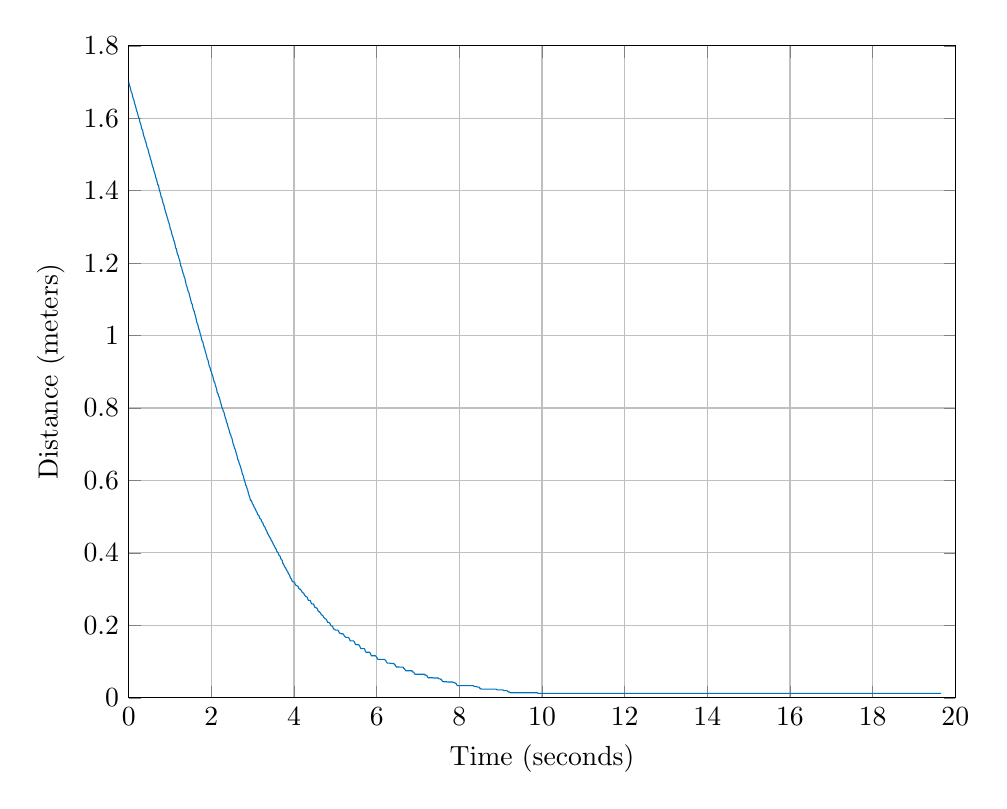
\begin{tikzpicture}

\begin{axis}[%
width=4.133in,
height=3.26in,
at={(0.693in,0.44in)},
scale only axis,
xmin=0,
xmax=20,
xmajorgrids,
xlabel={Time (seconds)},
ymin=0,
ymax=1.8,
ymajorgrids,
ylabel={Distance (meters)},
axis background/.style={fill=white}
]
\addplot [color=mycolor1,solid,forget plot]
  table[row sep=crcr]{%
0	1.70070346345311\\
0.0159777239999995	1.69086623549288\\
0.0321090869999975	1.68694606942081\\
0.0481079189999998	1.67910814535925\\
0.0640590819999985	1.67126980358659\\
0.0800937399999984	1.66931025400019\\
0.0961115539999977	1.65951269215463\\
0.112059099999998	1.65363385007974\\
0.128095164999999	1.64931765844527\\
0.144107822999999	1.63987454174872\\
0.16022602	1.63595492795775\\
0.176436053999998	1.62811765642852\\
0.192274968999997	1.62028010937229\\
0.208312000999998	1.61636077546817\\
0.224445437998999	1.60852406538375\\
0.240256767999999	1.60264594927523\\
0.256235530999999	1.59832898334341\\
0.272246213999998	1.58888312619996\\
0.288256415999997	1.58496382814955\\
0.304284272999998	1.57712743782508\\
0.320100665999997	1.56929053311861\\
0.336138408999998	1.56733139961559\\
0.352117502	1.55753558024245\\
0.368261987999998	1.54969907825446\\
0.384245494999997	1.54613077989034\\
0.400415454	1.53789213540846\\
0.416190528999999	1.53397324077266\\
0.432241748999998	1.52613738235538\\
0.448555228	1.51830131681099\\
0.464279937998999	1.51634227443859\\
0.480295162	1.50654744408871\\
0.49611382	1.5006704266809\\
0.512098092999998	1.49514035442108\\
0.528080552999999	1.48690123397875\\
0.544258044	1.48298268579319\\
0.560240717999998	1.47514768322867\\
0.576125136	1.46731231043609\\
0.592136877	1.46339418756768\\
0.608087463000998	1.45555948716013\\
0.624155911998998	1.44968297377696\\
0.640162150999997	1.44414956916429\\
0.656130693	1.435910793922\\
0.67221327	1.43199260880842\\
0.68816977	1.42415826163431\\
0.704135465999998	1.41632363508731\\
0.720146831	1.41436497297949\\
0.736124138999999	1.40457209797902\\
0.752133623999998	1.39829014301762\\
0.768111457999997	1.39275499500338\\
0.784161891999997	1.38296187724803\\
0.800203063999999	1.38100274330014\\
0.815989068	1.37316918514025\\
0.832085289999999	1.36533528603085\\
0.848108046	1.36141793146981\\
0.864191298	1.35358480038007\\
0.880130037999999	1.34608643900443\\
0.896134327	1.33980530655271\\
0.912191801999997	1.33393075027502\\
0.928191123999998	1.32805514303883\\
0.944326538999997	1.32218050962173\\
0.960005068999998	1.31434729718399\\
0.975954465999998	1.31043030750969\\
0.994062927999999	1.30259820302532\\
1.008973902	1.29273261691757\\
1.024018673	1.29077421622775\\
1.04210057	1.28098296194298\\
1.057133716	1.27510805200319\\
1.072491786	1.27119213207775\\
1.088189691	1.26335984388454\\
1.104071191	1.25944315419837\\
1.12011525	1.25161148210253\\
1.136083732	1.24174254875148\\
1.152086726001	1.23978431349393\\
1.168159963	1.2299941425369\\
1.18416712	1.224119721145\\
1.200112557	1.22020432742915\\
1.216133777	1.21237260627333\\
1.232151	1.20845649472547\\
1.248162628	1.19939812090512\\
1.264100654	1.19075307292089\\
1.280134106	1.18879499203392\\
1.296260263	1.17900576464386\\
1.312368036	1.17313192052206\\
1.328273386	1.16921675702218\\
1.344277093	1.16138619879248\\
1.360264749	1.1574700887325\\
1.376308177	1.14800392007756\\
1.392147707	1.13976389243298\\
1.408238111	1.13584790561907\\
1.424364075	1.12801779537965\\
1.440368358999	1.12214464641739\\
1.45627411	1.11822994905229\\
1.472293187	1.11039970156443\\
1.488109279	1.10370422446892\\
1.504243933	1.09660546439822\\
1.520258225	1.0887753081103\\
1.536146811	1.0868177745682\\
1.55208722	1.07703046466286\\
1.568197089	1.07115775969259\\
1.584110902	1.06724357385537\\
1.600089497999	1.05941436547601\\
1.616132715	1.05426413414225\\
1.632093845	1.04561666651659\\
1.648256884	1.03582997647433\\
1.664125781	1.03387267106571\\
1.680166707999	1.02604345271057\\
1.696118547	1.01821439636613\\
1.712264117	1.01430054346054\\
1.728294474	1.00564679555746\\
1.744231731	1.00049942572653\\
1.760298086	0.992671247962231\\
1.776224423	0.984842604006746\\
1.792030927	0.982885537825442\\
1.807977945	0.975057419161353\\
1.824104358	0.967228630175049\\
1.84015205	0.963315275071055\\
1.856144402	0.954247590731266\\
1.872143137	0.949511238610434\\
1.888269326999	0.941683749932993\\
1.904259434	0.933856074035005\\
1.920210107	0.931899128073447\\
1.936167358001	0.922114519337754\\
1.953769552	0.914287764321305\\
1.968766098	0.911917798954209\\
1.984172512	0.902848300216701\\
2.000055557	0.900480960564186\\
2.016107328	0.892653756780975\\
2.032082961	0.888739577896366\\
2.047948488	0.880913274758025\\
2.064123039	0.873086674282498\\
2.080253094	0.871129944704542\\
2.096106396	0.862890028866156\\
2.112099098	0.857731258489418\\
2.128102315	0.851450482460543\\
2.144102394	0.841667331314645\\
2.160072154	0.839710971400591\\
2.176111929	0.831884634581978\\
2.192199842	0.829928337107122\\
2.208235672	0.822102820506799\\
2.22406288	0.814276337703998\\
2.240190417	0.808702066723569\\
2.256381073	0.800463858163385\\
2.272243385	0.798507417931363\\
2.288173135	0.790681723470003\\
2.304232829	0.788725835021385\\
2.320228102999	0.780900367313005\\
2.33633977	0.773074463440338\\
2.352253288	0.769162924516195\\
2.368221054	0.760087812582637\\
2.384249517	0.75771603544379\\
2.40028206	0.74947795513265\\
2.416263878	0.743609588276014\\
2.432302685	0.737740778196293\\
2.448240964	0.729916319128132\\
2.464114858	0.727960841427103\\
2.480115784	0.720136244974353\\
2.496100107	0.716927748025705\\
2.512297197	0.708687234809073\\
2.528419017	0.700448375623395\\
2.544588425	0.696536864507616\\
2.56024656	0.688713262554401\\
2.576245436	0.686757258129132\\
2.592238885	0.678933453940243\\
2.608111827	0.673066899952459\\
2.624051364	0.665943299117577\\
2.640230033	0.657702387033726\\
2.656347784	0.655332088201222\\
2.672496138	0.647508656759513\\
2.688116818	0.643596866497596\\
2.704089786	0.637730019368293\\
2.720099818001	0.631863276628232\\
2.736095838	0.625995776470785\\
2.752089863	0.616915694638346\\
2.768088439	0.614541859925255\\
2.78412451	0.606303189037359\\
2.800109725	0.600436414331393\\
2.816095106	0.594569931012739\\
2.832099886	0.586747375831654\\
2.848126155	0.584792259096338\\
2.864113966	0.576970888468795\\
2.880085315	0.573754539108983\\
2.896158973	0.563558302236105\\
2.912117762	0.559230943131185\\
2.928091967	0.553364319830028\\
2.946335038	0.54554235001415\\
2.960220531999	0.545542626862491\\
2.975997723	0.541631860275187\\
2.994035466	0.535765237390957\\
3.008886524	0.533809744117906\\
3.023980285	0.529898904330135\\
3.040050652	0.524725700020631\\
3.058409402	0.522350969621772\\
3.073724191	0.518440129834001\\
3.089057911	0.514529073423288\\
3.104220408	0.512156732511877\\
3.120129546	0.506290913522093\\
3.136087775	0.504334836313393\\
3.152204474	0.502379343040342\\
3.168175214	0.496513524050558\\
3.184063869	0.494557446841859\\
3.200324903	0.492601953568808\\
3.216389118	0.486736134579024\\
3.232121376	0.484780057370324\\
3.248099049	0.482402596895119\\
3.264245274	0.475696597208698\\
3.280228671	0.47332128287419\\
3.296186249	0.47136578960114\\
3.31226691	0.465499970611355\\
3.328344535	0.463127045764295\\
3.344470665	0.459216279176991\\
3.360073559	0.453349656292761\\
3.376284316	0.45139416301971\\
3.392086220999	0.447483323231939\\
3.408085408	0.443572266821226\\
3.424105297	0.441616773548175\\
3.440095219	0.437705933760405\\
3.456060304	0.433372910147537\\
3.474233666	0.430577236177849\\
3.48923155	0.426247159264271\\
3.50429394	0.422336102853558\\
3.520112883	0.420380609580507\\
3.536269312001	0.416052922154376\\
3.552108657	0.412141865743663\\
3.568248563	0.410186372470612\\
3.584194204	0.404320553480828\\
3.600108905	0.402364476272128\\
3.616185723	0.400408982999077\\
3.632097821	0.394543164009293\\
3.648037896	0.392587086800594\\
3.664125245	0.390631593527543\\
3.679971729	0.383923205069124\\
3.698163256	0.381547549430267\\
3.713224225	0.379172819031409\\
3.728268674	0.371350922832925\\
3.744603386	0.369395429559874\\
3.760268757	0.365067742133743\\
3.776252349	0.36115668572303\\
3.792154195	0.359201192449979\\
3.808297753999	0.355290352662208\\
3.824360982	0.351379296251495\\
3.840176183	0.349423802978445\\
3.856079076999	0.345512963190674\\
3.872079837	0.341601906779961\\
3.88809921	0.339224446304756\\
3.90416367	0.334473425820348\\
3.920101959	0.330143132283827\\
3.936103893	0.328187639010777\\
3.953505749	0.322321820020992\\
3.968727644	0.320365742812293\\
3.984195998	0.319948895173932\\
4.000113279999	0.319948895173932\\
4.016112503	0.317993401900881\\
4.032108232001	0.312127582911097\\
4.048112469	0.310171505702398\\
4.064017835	0.310171505702398\\
4.080125713001	0.308216012429347\\
4.096168279	0.308216012429347\\
4.112117368	0.302350193439562\\
4.128101065	0.300394116230863\\
4.144104746999	0.300394116230863\\
4.16009529	0.298438622957813\\
4.176244918	0.296483056484296\\
4.192233922	0.292572803968028\\
4.208116128999	0.290194759557174\\
4.224219618	0.289774157290695\\
4.24030085	0.287399085587486\\
4.256306613	0.283069008673908\\
4.272276609	0.281114029471894\\
4.288177348	0.279157952263195\\
4.304241251	0.279157952263195\\
4.320323251	0.277202458990144\\
4.336301852	0.27133664000036\\
4.352112322	0.2689637151533\\
4.368048416	0.2689637151533\\
4.384087213	0.2689637151533\\
4.400094954	0.267008221880249\\
4.416085697	0.261142402890465\\
4.432098616	0.259186325681765\\
4.448237735	0.259186325681765\\
4.464175503	0.259186325681765\\
4.480095395	0.257230832408714\\
4.496126529999	0.25136501341893\\
4.512102179	0.249408936210231\\
4.528148673	0.249408936210231\\
4.543985698	0.24745344293718\\
4.559953039	0.247031475735025\\
4.575984265	0.241165656745241\\
4.591962851	0.238369398839904\\
4.608247046	0.238369398839904\\
4.624348931	0.235994668441046\\
4.640116824	0.234039101967529\\
4.656129131	0.230128849451261\\
4.672087406	0.228172772242562\\
4.688260842	0.228172772242562\\
4.704292027	0.225800431331151\\
4.72024058	0.22188959154338\\
4.736289364	0.219934612341366\\
4.752277877	0.217978535132667\\
4.768277055	0.217978535132667\\
4.784291445999	0.216023041859616\\
4.800018635	0.212112202071845\\
4.816296806	0.208201145661133\\
4.832195334	0.208201145661133\\
4.848246475	0.208201145661133\\
4.864267708	0.206245652388082\\
4.880089121999	0.202334812600311\\
4.896055935	0.198423756189598\\
4.912233101	0.198423756189598\\
4.928344237	0.198001788987443\\
4.944393427	0.193670126974396\\
4.961718553	0.189759874458129\\
4.976874884001	0.189340296027971\\
4.992295793	0.187384218819272\\
5.008099858001	0.186964981693464\\
5.024087354	0.186964981693464\\
5.040159537	0.186964981693464\\
5.056114068	0.186964981693464\\
5.072159344	0.185009488420413\\
5.088159469	0.181098648632643\\
5.104143301	0.179143669430629\\
5.120154876	0.17718759222193\\
5.136144642	0.17718759222193\\
5.152101103	0.176770744583569\\
5.168098661	0.176770744583569\\
5.184127656	0.176770744583569\\
5.200091984	0.174815251310518\\
5.216077023999	0.170904411522747\\
5.232104464999	0.168949432320734\\
5.250590581	0.166993355112034\\
5.265640408	0.166993355112034\\
5.280804437999	0.166993355112034\\
5.296168947	0.166993355112034\\
5.312194178	0.166993355112034\\
5.328174543	0.165037861838984\\
5.344271256	0.161127022051213\\
5.360290408	0.1572159656405\\
5.3762937	0.1572159656405\\
5.39225227	0.1572159656405\\
5.408216699	0.1572159656405\\
5.424320493	0.1572159656405\\
5.440259554	0.1572159656405\\
5.456272963001	0.155260472367449\\
5.472278355	0.151349632579679\\
5.488316941	0.147016608966811\\
5.50446695	0.147016608966811\\
5.5202356	0.147016608966811\\
5.536191975	0.146596006700331\\
5.552063889	0.146596006700331\\
5.568096858	0.146176428270174\\
5.584095901	0.144220934997123\\
5.600086046	0.139890858083545\\
5.616145284001	0.135979801672832\\
5.632130981	0.135979801672832\\
5.648264167	0.135979801672832\\
5.664117593	0.135979801672832\\
5.680122785	0.135979801672832\\
5.696124557	0.135979801672832\\
5.712126857	0.134024308399781\\
5.728099599	0.12774054376495\\
5.744203408	0.125785564562936\\
5.760259259	0.125785564562936\\
5.776226444	0.125785564562936\\
5.792139841	0.125785564562936\\
5.80810212	0.125785564562936\\
5.824077478	0.125785564562936\\
5.840078048001	0.123830071289886\\
5.856066896	0.119918427607669\\
5.872029642	0.116008175091402\\
5.888096402	0.116008175091402\\
5.904377142	0.116008175091402\\
5.920268064	0.116008175091402\\
5.936240811	0.116008175091402\\
5.95416099	0.116008175091402\\
5.969498242	0.116008175091402\\
5.985008788	0.114052681818351\\
6.000421863	0.112096604609651\\
6.016104768	0.108185764821881\\
6.032255534	0.106230785619867\\
6.048244167	0.106230785619867\\
6.064238358	0.106230785619867\\
6.080274393	0.106230785619867\\
6.096286184	0.106230785619867\\
6.112102527	0.106230785619867\\
6.128365231	0.106230785619867\\
6.144091896001	0.106230785619867\\
6.160252649	0.106230785619867\\
6.176303499	0.106230785619867\\
6.192278717	0.105808818417713\\
6.208381203	0.103853325144662\\
6.224280313	0.101897247935963\\
6.240256969	0.0979864081481916\\
6.256243878	0.0960314289461781\\
6.272113878	0.0956108266796987\\
6.288178428	0.0956108266796987\\
6.304001469	0.0956108266796987\\
6.320088728	0.0956108266796987\\
6.336314454	0.0951912482495412\\
6.3522912	0.0951912482495412\\
6.368237462	0.0951912482495412\\
6.384265349	0.0947720111237333\\
6.400370241	0.0947720111237333\\
6.416093924	0.0947720111237333\\
6.4320925	0.0908604406419835\\
6.448241932	0.0908604406419835\\
6.464177155	0.0869496008542123\\
6.480089931	0.0849946216521988\\
6.496066983	0.0849946216521988\\
6.51211214	0.0849946216521988\\
6.528241467	0.0849946216521988\\
6.544276731	0.0849946216521988\\
6.560089761	0.084577774013838\\
6.576070131	0.084577774013838\\
6.592084267	0.084577774013838\\
6.608270642999	0.084577774013838\\
6.624230215	0.084577774013838\\
6.640371233999	0.084577774013838\\
6.656293918	0.080666203532088\\
6.672419566	0.080666203532088\\
6.688118042001	0.076755363744317\\
6.704094548	0.0748003845423035\\
6.720247910001	0.0748003845423035\\
6.736293216	0.0748003845423035\\
6.752118665	0.0748003845423035\\
6.768093898	0.0748003845423035\\
6.784105829	0.0748003845423035\\
6.800233983	0.0748003845423035\\
6.816268505	0.0748003845423035\\
6.83221159	0.0748003845423035\\
6.848086276	0.0748003845423035\\
6.864117094	0.0728443073336045\\
6.880269113	0.0708888140605537\\
6.896338679	0.0708888140605537\\
6.912140459	0.066977974272783\\
6.928093727	0.0650229950707693\\
6.944177697	0.0650229950707693\\
6.961630842	0.0650229950707693\\
6.976705595	0.0650229950707693\\
6.992307027	0.0650229950707693\\
7.008268574	0.0650229950707693\\
7.024037568	0.0650229950707693\\
7.040151211	0.0650229950707693\\
7.056142565	0.0650229950707693\\
7.072270509	0.0650229950707693\\
7.088155834	0.0650229950707693\\
7.104108906	0.0650229950707693\\
7.120224317	0.0650229950707693\\
7.136114783	0.0650229950707693\\
7.152237389	0.0650229950707693\\
7.168329688	0.06306691786207\\
7.18434001	0.06306691786207\\
7.200266803	0.0611114245890192\\
7.216262993	0.0611114245890192\\
7.232028907	0.0572005848012482\\
7.250248364	0.0552456055992347\\
7.265570975001	0.0552456055992347\\
7.281339102	0.0552456055992347\\
7.297183113	0.0552456055992347\\
7.312662167	0.0552456055992347\\
7.328281403	0.0552456055992347\\
7.344266809	0.0552456055992347\\
7.360272481	0.0552456055992347\\
7.37625896	0.0548236383970802\\
7.392298874	0.0548236383970802\\
7.408251335	0.0548236383970802\\
7.424108556	0.0548236383970802\\
7.440263530999	0.0548236383970802\\
7.456209778	0.0548236383970802\\
7.472318323	0.0548236383970802\\
7.488248474	0.0548236383970802\\
7.504262675	0.0524469589219017\\
7.520283463	0.0524469589219017\\
7.536179692001	0.0524469589219017\\
7.552479413	0.0504914656488509\\
7.568254261999	0.0504914656488509\\
7.58438835	0.0465806258610799\\
7.600412131	0.0446256466590664\\
7.616258714	0.0446256466590664\\
7.632253231	0.0442060682289087\\
7.64828426	0.0442060682289087\\
7.664125595	0.0442060682289087\\
7.680164306	0.0442060682289087\\
7.696105487	0.0442060682289087\\
7.712163162	0.0437868311031009\\
7.728110132	0.0437868311031009\\
7.744049321	0.0437868311031009\\
7.760126581	0.0437868311031009\\
7.776148991	0.0437868311031009\\
7.792165743	0.0437868311031009\\
7.808046159	0.0437868311031009\\
7.824043769	0.0437868311031009\\
7.840093306	0.0437868311031009\\
7.856154118	0.0418307538944016\\
7.872132398	0.0418307538944016\\
7.888141176	0.0418307538944016\\
7.904200374	0.0398752606213508\\
7.920136604	0.0398752606213508\\
7.93615076	0.0359644208335801\\
7.953456651	0.0335925939932056\\
7.968391552	0.0335925939932056\\
7.98406813	0.0335925939932056\\
8.000115071	0.0335925939932056\\
8.016118283	0.0335925939932056\\
8.032268877	0.0335925939932056\\
8.048431685	0.0335925939932056\\
8.064168181999	0.0335925939932056\\
8.080184618	0.0335925939932056\\
8.096195196	0.0335925939932056\\
8.11215072	0.0335925939932056\\
8.128133088	0.0335925939932056\\
8.144044822	0.0335925939932056\\
8.160124317	0.0335925939932056\\
8.176154679	0.0335925939932056\\
8.192137891	0.0335925939932056\\
8.208157659	0.0335925939932056\\
8.224159458	0.0335925939932056\\
8.240219558	0.0335925939932056\\
8.256082652	0.0335925939932056\\
8.27199661	0.0335925939932056\\
8.288092987	0.0335925939932056\\
8.304190633	0.0335925939932056\\
8.320243181	0.0335925939932056\\
8.336155421	0.0335925939932056\\
8.352194193	0.0316365167845065\\
8.368273070999	0.0316365167845065\\
8.384222294999	0.0316365167845065\\
8.400181346	0.0316365167845065\\
8.416134484	0.0316365167845065\\
8.432155631	0.029681023511456\\
8.448128193	0.029681023511456\\
8.464156606	0.029681023511456\\
8.480154003999	0.029681023511456\\
8.496266208	0.025770183723685\\
8.512111431	0.025770183723685\\
8.528266647	0.0238152045216715\\
8.544314674	0.0238152045216715\\
8.560297364	0.0238152045216715\\
8.576287867	0.0238152045216715\\
8.592279036	0.0238152045216715\\
8.608080370001	0.0238152045216715\\
8.624265032	0.0238152045216715\\
8.640275169	0.0238152045216715\\
8.656299218001	0.0238152045216715\\
8.672308287	0.0238152045216715\\
8.688181579	0.0238152045216715\\
8.704377006	0.0238152045216715\\
8.720117572	0.0238152045216715\\
8.736222895	0.0238152045216715\\
8.752169197	0.0238152045216715\\
8.768185725	0.0238152045216715\\
8.784069627	0.0238152045216715\\
8.800054688	0.0238152045216715\\
8.816013448	0.0238152045216715\\
8.832268046	0.0238152045216715\\
8.848122862	0.0238152045216715\\
8.864161333	0.0238152045216715\\
8.880146012	0.0238152045216715\\
8.896107219	0.0238152045216715\\
8.91218809	0.021859127312972\\
8.928099663	0.021859127312972\\
8.944129055	0.021859127312972\\
8.960250881	0.021859127312972\\
8.976348519	0.021859127312972\\
8.992208452	0.021859127312972\\
9.008062036	0.021859127312972\\
9.024159369	0.021859127312972\\
9.040162043	0.021859127312972\\
9.056263187	0.021859127312972\\
9.072157797	0.0199036340399212\\
9.088168295	0.0199036340399212\\
9.104227889	0.0199036340399212\\
9.120096475	0.0199036340399212\\
9.136108015	0.0199036340399212\\
9.152090525	0.0199036340399212\\
9.168090724	0.0179483607256676\\
9.184097148	0.0159927942521505\\
9.20007414	0.0159927942521505\\
9.21610561	0.0159927942521505\\
9.232149016999	0.0140378150501368\\
9.248159686	0.0140378150501368\\
9.26415994	0.0140378150501368\\
9.280191446	0.0140378150501368\\
9.296171354	0.0140378150501368\\
9.312116955	0.0140378150501368\\
9.328143584	0.0140378150501368\\
9.344119379	0.0140378150501368\\
9.360432813	0.0140378150501368\\
9.376183412	0.0140378150501368\\
9.39215687	0.0140378150501368\\
9.408143063	0.0140378150501368\\
9.424167718	0.0140378150501368\\
9.440152462	0.0140378150501368\\
9.456159047	0.0140378150501368\\
9.472144502	0.0140378150501368\\
9.488135505	0.0140378150501368\\
9.50412233	0.0140378150501368\\
9.520103447	0.0140378150501368\\
9.536119412	0.0140378150501368\\
9.552133588	0.0140378150501368\\
9.568055895	0.0140378150501368\\
9.584151442	0.0140378150501368\\
9.600121172	0.0140378150501368\\
9.616112997	0.0140378150501368\\
9.632090316	0.0140378150501368\\
9.648149257	0.0140378150501368\\
9.664049222	0.0140378150501368\\
9.680137715	0.0140378150501368\\
9.696147085	0.0140378150501368\\
9.712129058	0.0140378150501368\\
9.728254772001	0.0140378150501368\\
9.744174063	0.0140378150501368\\
9.760166304	0.0140378150501368\\
9.776138942	0.0140378150501368\\
9.792132992	0.0140378150501368\\
9.808182198	0.0140378150501368\\
9.824162758	0.0140378150501368\\
9.84018215	0.0140378150501368\\
9.856214974	0.0140378150501368\\
9.872098304	0.0140378150501368\\
9.888116734	0.0140378150501368\\
9.904078161	0.0120817378414375\\
9.920110408	0.0120817378414375\\
9.936068382	0.0120817378414375\\
9.954008335	0.0120817378414375\\
9.969494926	0.0120817378414375\\
9.984763203	0.0120817378414375\\
10.0001576	0.0120817378414375\\
10.016058485	0.0120817378414375\\
10.032128507	0.0120817378414375\\
10.048063225	0.0120817378414375\\
10.066290568	0.0120817378414375\\
10.081778016001	0.0120817378414375\\
10.097111305	0.0120817378414375\\
10.112814496	0.0120817378414375\\
10.128169745	0.0120817378414375\\
10.144215469	0.0120817378414375\\
10.160370402	0.0120817378414375\\
10.176183628	0.0120817378414375\\
10.192149372	0.0120817378414375\\
10.208330033	0.0120817378414375\\
10.224134609	0.0120817378414375\\
10.240122225	0.0120817378414375\\
10.256418165	0.0120817378414375\\
10.272231312999	0.0120817378414375\\
10.288143616	0.0120817378414375\\
10.304347546	0.0120817378414375\\
10.320193747	0.0120817378414375\\
10.336127157	0.0120817378414375\\
10.352138379999	0.0120817378414375\\
10.368185187001	0.0120817378414375\\
10.38418979	0.0120817378414375\\
10.400215311	0.0120817378414375\\
10.416189903	0.0120817378414375\\
10.432085871	0.0120817378414375\\
10.448100393	0.0120817378414375\\
10.464160708999	0.0120817378414375\\
10.480122927	0.0120817378414375\\
10.496115554	0.0120817378414375\\
10.512099167	0.0120817378414375\\
10.528102749	0.0120817378414375\\
10.544173107	0.0120817378414375\\
10.560101744	0.0120817378414375\\
10.576041276	0.0120817378414375\\
10.592229812999	0.0120817378414375\\
10.60840134	0.0120817378414375\\
10.624268338001	0.0120817378414375\\
10.640122747	0.0120817378414375\\
10.656125377001	0.0120817378414375\\
10.672257199	0.0120817378414375\\
10.68836583	0.0120817378414375\\
10.704248347	0.0120817378414375\\
10.720252962	0.0120817378414375\\
10.736536043	0.0120817378414375\\
10.752283439	0.0120817378414375\\
10.768305393	0.0120817378414375\\
10.784119406	0.0120817378414375\\
10.800050331	0.0120817378414375\\
10.816099163	0.0120817378414375\\
10.832273111	0.0120817378414375\\
10.84826898	0.0120817378414375\\
10.8641012	0.0120817378414375\\
10.880083668999	0.0120817378414375\\
10.89609571	0.0120817378414375\\
10.912121723	0.0120817378414375\\
10.928229590999	0.0120817378414375\\
10.944229104	0.0120817378414375\\
10.961943987	0.0120817378414375\\
10.978185314	0.0120817378414375\\
10.993472378	0.0120817378414375\\
11.009054404999	0.0120817378414375\\
11.024576592	0.0120817378414375\\
11.040438137	0.0120817378414375\\
11.056240083	0.0120817378414375\\
11.072238448	0.0120817378414375\\
11.088084047	0.0120817378414375\\
11.104279338	0.0120817378414375\\
11.14056567	0.0120817378414375\\
11.156090263	0.0120817378414375\\
11.174180867	0.0120817378414375\\
11.189216217	0.0120817378414375\\
11.204138304	0.0120817378414375\\
11.220094718	0.0120817378414375\\
11.236247585	0.0120817378414375\\
11.252081463	0.0120817378414375\\
11.268131472	0.0120817378414375\\
11.284185857	0.0120817378414375\\
11.301197757	0.0120817378414375\\
11.31617367	0.0120817378414375\\
11.332097319	0.0120817378414375\\
11.348133169	0.0120817378414375\\
11.364154925	0.0120817378414375\\
11.38018726	0.0120817378414375\\
11.396321416	0.0120817378414375\\
11.41247177	0.0120817378414375\\
11.428266431	0.0120817378414375\\
11.444498516	0.0120817378414375\\
11.460372850001	0.0120817378414375\\
11.476181217	0.0120817378414375\\
11.492497469	0.0120817378414375\\
11.50833055	0.0120817378414375\\
11.524244565	0.0120817378414375\\
11.540323808	0.0120817378414375\\
11.556233861	0.0120817378414375\\
11.57227684	0.0120817378414375\\
11.588206124	0.0120817378414375\\
11.604147515	0.0120817378414375\\
11.622519212	0.0120817378414375\\
11.637746065	0.0120817378414375\\
11.653107362	0.0120817378414375\\
11.668552499	0.0120817378414375\\
11.684533377	0.0120817378414375\\
11.700522194	0.0120817378414375\\
11.716316141	0.0120817378414375\\
11.732343737	0.0120817378414375\\
11.748186825001	0.0120817378414375\\
11.764164739	0.0120817378414375\\
11.78269695	0.0120817378414375\\
11.797938659	0.0120817378414375\\
11.813895397	0.0120817378414375\\
11.829170168	0.0120817378414375\\
11.844443805	0.0120817378414375\\
11.86017635	0.0120817378414375\\
11.876329752	0.0120817378414375\\
11.892193963	0.0120817378414375\\
11.908258539	0.0120817378414375\\
11.924289037	0.0120817378414375\\
11.940230408	0.0120817378414375\\
11.957686646	0.0120817378414375\\
11.972635829	0.0120817378414375\\
11.988202807	0.0120817378414375\\
12.004110929	0.0120817378414375\\
12.020174541	0.0120817378414375\\
12.036210823	0.0120817378414375\\
12.052244197	0.0120817378414375\\
12.068197732	0.0120817378414375\\
12.084263905	0.0120817378414375\\
12.100114284	0.0120817378414375\\
12.118373416	0.0120817378414375\\
12.133537372	0.0120817378414375\\
12.148756377001	0.0120817378414375\\
12.164161323	0.0120817378414375\\
12.180420499	0.0120817378414375\\
12.196166312	0.0120817378414375\\
12.212328503999	0.0120817378414375\\
12.228268632	0.0120817378414375\\
12.244299015	0.0120817378414375\\
12.260200494	0.0120817378414375\\
12.276425173	0.0120817378414375\\
12.292235112	0.0120817378414375\\
12.308182512	0.0120817378414375\\
12.32422837	0.0120817378414375\\
12.340138043	0.0120817378414375\\
12.356086801	0.0120817378414375\\
12.372273815	0.0120817378414375\\
12.388308718	0.0120817378414375\\
12.416152325	0.0120817378414375\\
12.421598838	0.0120817378414375\\
12.436787575	0.0120817378414375\\
12.452107865	0.0120817378414375\\
12.470407512	0.0120817378414375\\
12.485587789	0.0120817378414375\\
12.500756035	0.0120817378414375\\
12.51622933	0.0120817378414375\\
12.532286183	0.0120817378414375\\
12.550672483	0.0120817378414375\\
12.565836232	0.0120817378414375\\
12.581019766999	0.0120817378414375\\
12.596378906	0.0120817378414375\\
12.612486994	0.0120817378414375\\
12.628237858	0.0120817378414375\\
12.644281656	0.0120817378414375\\
12.660331654	0.0120817378414375\\
12.676280739	0.0120817378414375\\
12.703150408	0.0120817378414375\\
12.708526156	0.0120817378414375\\
12.724101477	0.0120817378414375\\
12.740080173	0.0120817378414375\\
12.756338874	0.0120817378414375\\
12.77223381	0.0120817378414375\\
12.78832044	0.0120817378414375\\
12.80429664	0.0120817378414375\\
12.820262221	0.0120817378414375\\
12.836253291	0.0120817378414375\\
12.852412891	0.0120817378414375\\
12.868279262	0.0120817378414375\\
12.884276705	0.0120817378414375\\
12.900277666	0.0120817378414375\\
12.916333154	0.0120817378414375\\
12.932280902	0.0120817378414375\\
12.951023434	0.0120817378414375\\
12.964155696	0.0120817378414375\\
12.98013903	0.0120817378414375\\
12.996303048	0.0120817378414375\\
13.012175142	0.0120817378414375\\
13.028327885	0.0120817378414375\\
13.044290782	0.0120817378414375\\
13.060159394	0.0120817378414375\\
13.076308029	0.0120817378414375\\
13.092347969	0.0120817378414375\\
13.108220809	0.0120817378414375\\
13.124361052	0.0120817378414375\\
13.140234409	0.0120817378414375\\
13.156290234	0.0120817378414375\\
13.172214176	0.0120817378414375\\
13.188287306	0.0120817378414375\\
13.204185253	0.0120817378414375\\
13.220255281	0.0120817378414375\\
13.236193671	0.0120817378414375\\
13.252252323	0.0120817378414375\\
13.268258636	0.0120817378414375\\
13.284257182	0.0120817378414375\\
13.300331759	0.0120817378414375\\
13.316196617	0.0120817378414375\\
13.332258822	0.0120817378414375\\
13.348353904	0.0120817378414375\\
13.364175872	0.0120817378414375\\
13.38025882	0.0120817378414375\\
13.396199319	0.0120817378414375\\
13.41227738	0.0120817378414375\\
13.428234832999	0.0120817378414375\\
13.444295348	0.0120817378414375\\
13.460343276	0.0120817378414375\\
13.476438550999	0.0120817378414375\\
13.492245452	0.0120817378414375\\
13.50816392	0.0120817378414375\\
13.524122177	0.0120817378414375\\
13.540228055001	0.0120817378414375\\
13.556316334	0.0120817378414375\\
13.572316589	0.0120817378414375\\
13.588250618	0.0120817378414375\\
13.604291983001	0.0120817378414375\\
13.620190097	0.0120817378414375\\
13.6361217	0.0120817378414375\\
13.652272262	0.0120817378414375\\
13.668281894	0.0120817378414375\\
13.684268355	0.0120817378414375\\
13.700246159	0.0120817378414375\\
13.716207568	0.0120817378414375\\
13.732278833999	0.0120817378414375\\
13.748399904001	0.0120817378414375\\
13.764214546	0.0120817378414375\\
13.780229037	0.0120817378414375\\
13.796274304	0.0120817378414375\\
13.812579755	0.0120817378414375\\
13.828640161	0.0120817378414375\\
13.844227883	0.0120817378414375\\
13.860539406	0.0120817378414375\\
13.876630882	0.0120817378414375\\
13.892161578	0.0120817378414375\\
13.908248429	0.0120817378414375\\
13.924139106	0.0120817378414375\\
13.94022758	0.0120817378414375\\
13.958053117	0.0120817378414375\\
13.972995582	0.0120817378414375\\
13.988124967	0.0120817378414375\\
14.006194018	0.0120817378414375\\
14.021187427	0.0120817378414375\\
14.036132207999	0.0120817378414375\\
14.052262677	0.0120817378414375\\
14.068270574	0.0120817378414375\\
14.084324316	0.0120817378414375\\
14.100242004	0.0120817378414375\\
14.116124141	0.0120817378414375\\
14.132236188	0.0120817378414375\\
14.148514632	0.0120817378414375\\
14.164329497	0.0120817378414375\\
14.180282439	0.0120817378414375\\
14.196297292	0.0120817378414375\\
14.21225283	0.0120817378414375\\
14.228142407	0.0120817378414375\\
14.244184789	0.0120817378414375\\
14.26036428	0.0120817378414375\\
14.276303892	0.0120817378414375\\
14.292238047	0.0120817378414375\\
14.308275105	0.0120817378414375\\
14.324231906	0.0120817378414375\\
14.340255423001	0.0120817378414375\\
14.356290231	0.0120817378414375\\
14.372225053	0.0120817378414375\\
14.388090671	0.0120817378414375\\
14.404091663	0.0120817378414375\\
14.420078015	0.0120817378414375\\
14.436164222	0.0120817378414375\\
14.452075807999	0.0120817378414375\\
14.468313752001	0.0120817378414375\\
14.484543567	0.0120817378414375\\
14.500343447	0.0120817378414375\\
14.516236192	0.0120817378414375\\
14.532252285	0.0120817378414375\\
14.550682752	0.0120817378414375\\
14.564550373	0.0120817378414375\\
14.580319604	0.0120817378414375\\
14.596207800999	0.0120817378414375\\
14.612185558	0.0120817378414375\\
14.628232995	0.0120817378414375\\
14.644294259	0.0120817378414375\\
14.660120663	0.0120817378414375\\
14.676255578	0.0120817378414375\\
14.692271829	0.0120817378414375\\
14.708314019	0.0120817378414375\\
14.724199223	0.0120817378414375\\
14.740246108	0.0120817378414375\\
14.75630274	0.0120817378414375\\
14.77227455	0.0120817378414375\\
14.788313034	0.0120817378414375\\
14.804285669	0.0120817378414375\\
14.820375551	0.0120817378414375\\
14.83627178	0.0120817378414375\\
14.85218547	0.0120817378414375\\
14.868286826999	0.0120817378414375\\
14.884208337	0.0120817378414375\\
14.90033553	0.0120817378414375\\
14.916228612	0.0120817378414375\\
14.932255257	0.0120817378414375\\
14.953044645	0.0120817378414375\\
14.96482545	0.0120817378414375\\
14.980143421	0.0120817378414375\\
14.996097756	0.0120817378414375\\
15.01423209	0.0120817378414375\\
15.029268852	0.0120817378414375\\
15.044252895	0.0120817378414375\\
15.060202239	0.0120817378414375\\
15.076226613	0.0120817378414375\\
15.092176135	0.0120817378414375\\
15.108162427	0.0120817378414375\\
15.124364332	0.0120817378414375\\
15.140096146	0.0120817378414375\\
15.156291485	0.0120817378414375\\
15.172245811	0.0120817378414375\\
15.188173953	0.0120817378414375\\
15.204340934	0.0120817378414375\\
15.220095253	0.0120817378414375\\
15.238210708	0.0120817378414375\\
15.253333274	0.0120817378414375\\
15.268642744	0.0120817378414375\\
15.284201157	0.0120817378414375\\
15.30049381	0.0120817378414375\\
15.316306544	0.0120817378414375\\
15.332307305001	0.0120817378414375\\
15.348109325	0.0120817378414375\\
15.364111353	0.0120817378414375\\
15.380457477	0.0120817378414375\\
15.39628448	0.0120817378414375\\
15.412129321	0.0120817378414375\\
15.428196864	0.0120817378414375\\
15.444315452	0.0120817378414375\\
15.460265739001	0.0120817378414375\\
15.476253289	0.0120817378414375\\
15.492323703	0.0120817378414375\\
15.50812908	0.0120817378414375\\
15.524182221	0.0120817378414375\\
15.54008591	0.0120817378414375\\
15.556098878	0.0120817378414375\\
15.572264233	0.0120817378414375\\
15.588279411999	0.0120817378414375\\
15.604302207	0.0120817378414375\\
15.620271797	0.0120817378414375\\
15.636264475001	0.0120817378414375\\
15.652246573	0.0120817378414375\\
15.668276465	0.0120817378414375\\
15.684197117	0.0120817378414375\\
15.700285508	0.0120817378414375\\
15.716889881	0.0120817378414375\\
15.732216109	0.0120817378414375\\
15.748375434	0.0120817378414375\\
15.764282919	0.0120817378414375\\
15.780299148999	0.0120817378414375\\
15.796194646	0.0120817378414375\\
15.812341554	0.0120817378414375\\
15.828268913	0.0120817378414375\\
15.844289469001	0.0120817378414375\\
15.860223808	0.0120817378414375\\
15.876284766	0.0120817378414375\\
15.892257152001	0.0120817378414375\\
15.908444591	0.0120817378414375\\
15.924354357	0.0120817378414375\\
15.940240326	0.0120817378414375\\
15.957828668	0.0120817378414375\\
15.972815743	0.0120817378414375\\
15.988142807999	0.0120817378414375\\
16.006201298001	0.0120817378414375\\
16.021135685	0.0120817378414375\\
16.036148508	0.0120817378414375\\
16.052245953	0.0120817378414375\\
16.068270988	0.0120817378414375\\
16.084331602	0.0120817378414375\\
16.100333317	0.0120817378414375\\
16.116210332999	0.0120817378414375\\
16.132239308	0.0120817378414375\\
16.148543781	0.0120817378414375\\
16.164265931	0.0120817378414375\\
16.180324181999	0.0120817378414375\\
16.196204928	0.0120817378414375\\
16.212319239	0.0120817378414375\\
16.228195651	0.0120817378414375\\
16.24421434	0.0120817378414375\\
16.260441432	0.0120817378414375\\
16.276271848	0.0120817378414375\\
16.292262425	0.0120817378414375\\
16.308278842	0.0120817378414375\\
16.324271223	0.0120817378414375\\
16.34041397	0.0120817378414375\\
16.356299840999	0.0120817378414375\\
16.372287166	0.0120817378414375\\
16.388318973	0.0120817378414375\\
16.404333655	0.0120817378414375\\
16.420278509	0.0120817378414375\\
16.436177639	0.0120817378414375\\
16.452209525	0.0120817378414375\\
16.468215484999	0.0120817378414375\\
16.484138362	0.0120817378414375\\
16.500187832	0.0120817378414375\\
16.516194183	0.0120817378414375\\
16.532256823	0.0120817378414375\\
16.55074378	0.0120817378414375\\
16.565897152001	0.0120817378414375\\
16.581019001001	0.0120817378414375\\
16.596276569	0.0120817378414375\\
16.612288227	0.0120817378414375\\
16.628282114	0.0120817378414375\\
16.644285025	0.0120817378414375\\
16.66029454	0.0120817378414375\\
16.676269874	0.0120817378414375\\
16.692270469	0.0120817378414375\\
16.708322742	0.0120817378414375\\
16.724246535	0.0120817378414375\\
16.740262834	0.0120817378414375\\
16.756285134	0.0120817378414375\\
16.772271191	0.0120817378414375\\
16.788277369	0.0120817378414375\\
16.804235138	0.0120817378414375\\
16.820283556	0.0120817378414375\\
16.836267789	0.0120817378414375\\
16.852221047	0.0120817378414375\\
16.868287376	0.0120817378414375\\
16.884273484	0.0120817378414375\\
16.900344219001	0.0120817378414375\\
16.916230766	0.0120817378414375\\
16.932237665	0.0120817378414375\\
16.950719503	0.0120817378414375\\
16.965948426	0.0120817378414375\\
16.981222251	0.0120817378414375\\
16.996395298001	0.0120817378414375\\
17.01223971	0.0120817378414375\\
17.028223227	0.0120817378414375\\
17.044209444	0.0120817378414375\\
17.060232005	0.0120817378414375\\
17.076234549	0.0120817378414375\\
17.092245257	0.0120817378414375\\
17.108442754	0.0120817378414375\\
17.124253244	0.0120817378414375\\
17.140218845	0.0120817378414375\\
17.156278248	0.0120817378414375\\
17.17227295	0.0120817378414375\\
17.188298289	0.0120817378414375\\
17.204250218	0.0120817378414375\\
17.220274756	0.0120817378414375\\
17.23621662	0.0120817378414375\\
17.252282046	0.0120817378414375\\
17.268368882	0.0120817378414375\\
17.284252658	0.0120817378414375\\
17.300352954	0.0120817378414375\\
17.316279331	0.0120817378414375\\
17.332262777	0.0120817378414375\\
17.348250123	0.0120817378414375\\
17.364267361	0.0120817378414375\\
17.380333885999	0.0120817378414375\\
17.396273684	0.0120817378414375\\
17.412312781	0.0120817378414375\\
17.428266941	0.0120817378414375\\
17.444326265	0.0120817378414375\\
17.460334407	0.0120817378414375\\
17.476278454	0.0120817378414375\\
17.492360655	0.0120817378414375\\
17.508284325999	0.0120817378414375\\
17.524268162999	0.0120817378414375\\
17.540321107001	0.0120817378414375\\
17.556284358	0.0120817378414375\\
17.572271868	0.0120817378414375\\
17.588319987	0.0120817378414375\\
17.604261483	0.0120817378414375\\
17.620296692	0.0120817378414375\\
17.636232134	0.0120817378414375\\
17.652261771	0.0120817378414375\\
17.668308155	0.0120817378414375\\
17.684172168	0.0120817378414375\\
17.700343478	0.0120817378414375\\
17.716247074	0.0120817378414375\\
17.732256043	0.0120817378414375\\
17.750618333	0.0120817378414375\\
17.765867872	0.0120817378414375\\
17.781094103	0.0120817378414375\\
17.796344485	0.0120817378414375\\
17.812254856	0.0120817378414375\\
17.828165295	0.0120817378414375\\
17.844200946	0.0120817378414375\\
17.860142945	0.0120817378414375\\
17.876278134	0.0120817378414375\\
17.892296089	0.0120817378414375\\
17.90825522	0.0120817378414375\\
17.924223127	0.0120817378414375\\
17.940277246	0.0120817378414375\\
17.957852638	0.0120817378414375\\
17.972836437999	0.0120817378414375\\
17.988142337	0.0120817378414375\\
18.006234403	0.0120817378414375\\
18.021276106	0.0120817378414375\\
18.036463539	0.0120817378414375\\
18.052262082	0.0120817378414375\\
18.068293227	0.0120817378414375\\
18.084250385	0.0120817378414375\\
18.101171965	0.0120817378414375\\
18.116328283	0.0120817378414375\\
18.132266788	0.0120817378414375\\
18.148351063	0.0120817378414375\\
18.164278873	0.0120817378414375\\
18.18254261	0.0120817378414375\\
18.197660180001	0.0120817378414375\\
18.21274877	0.0120817378414375\\
18.228219515	0.0120817378414375\\
18.244212628999	0.0120817378414375\\
18.260159044	0.0120817378414375\\
18.276231143	0.0120817378414375\\
18.292220477999	0.0120817378414375\\
18.308276835	0.0120817378414375\\
18.324248791	0.0120817378414375\\
18.340272829	0.0120817378414375\\
18.356317003	0.0120817378414375\\
18.372178471	0.0120817378414375\\
18.388307053	0.0120817378414375\\
18.404259455	0.0120817378414375\\
18.420311146	0.0120817378414375\\
18.436235168	0.0120817378414375\\
18.452250902	0.0120817378414375\\
18.468277742	0.0120817378414375\\
18.484240131	0.0120817378414375\\
18.5027387	0.0120817378414375\\
18.518032594	0.0120817378414375\\
18.533480453	0.0120817378414375\\
18.548763884	0.0120817378414375\\
18.564309458	0.0120817378414375\\
18.580230644	0.0120817378414375\\
18.596282569999	0.0120817378414375\\
18.612272662	0.0120817378414375\\
18.628357047	0.0120817378414375\\
18.644254745001	0.0120817378414375\\
18.660326416	0.0120817378414375\\
18.676263244	0.0120817378414375\\
18.6922729	0.0120817378414375\\
18.708296185	0.0120817378414375\\
18.724229602	0.0120817378414375\\
18.740240316	0.0120817378414375\\
18.756300591	0.0120817378414375\\
18.772220359	0.0120817378414375\\
18.788283225	0.0120817378414375\\
18.804224471	0.0120817378414375\\
18.820393628	0.0120817378414375\\
18.836265547	0.0120817378414375\\
18.852210311	0.0120817378414375\\
18.868286015	0.0120817378414375\\
18.884192691	0.0120817378414375\\
18.900281910001	0.0120817378414375\\
18.916216767	0.0120817378414375\\
18.932238355	0.0120817378414375\\
18.953054333	0.0120817378414375\\
18.965077168	0.0120817378414375\\
18.980300121999	0.0120817378414375\\
18.996289752	0.0120817378414375\\
19.012262224	0.0120817378414375\\
19.028403072	0.0120817378414375\\
19.044271217	0.0120817378414375\\
19.060212335	0.0120817378414375\\
19.076279209	0.0120817378414375\\
19.092331951999	0.0120817378414375\\
19.108249244	0.0120817378414375\\
19.124247639	0.0120817378414375\\
19.140241329	0.0120817378414375\\
19.156325589	0.0120817378414375\\
19.172267135	0.0120817378414375\\
19.188352102	0.0120817378414375\\
19.204248696	0.0120817378414375\\
19.220303064	0.0120817378414375\\
19.236268886	0.0120817378414375\\
19.252241753	0.0120817378414375\\
19.268253233	0.0120817378414375\\
19.284270616	0.0120817378414375\\
19.300334711	0.0120817378414375\\
19.316229516	0.0120817378414375\\
19.332236376	0.0120817378414375\\
19.348436017	0.0120817378414375\\
19.364253478	0.0120817378414375\\
19.382716962	0.0120817378414375\\
19.397894478	0.0120817378414375\\
19.413063715	0.0120817378414375\\
19.428381243	0.0120817378414375\\
19.444259867	0.0120817378414375\\
19.460268351	0.0120817378414375\\
19.47627225	0.0120817378414375\\
19.492268995	0.0120817378414375\\
19.508304078	0.0120817378414375\\
19.524232526	0.0120817378414375\\
19.54021497	0.0120817378414375\\
19.556338554	0.0120817378414375\\
19.57224227	0.0120817378414375\\
19.588286975	0.0120817378414375\\
19.604291239	0.0120817378414375\\
19.620285084	0.0120817378414375\\
19.652273021	0.0120817378414375\\
19.657778083999	0.0120817378414375\\
};
\end{axis}
\end{tikzpicture}%
}
      \caption{The error in displacement of the robot over time for
        $(K_{\Psi}^R, K_{\omega}^T) \equiv (0.2 K_{\Psi, max}^R, 0.2 K_{\omega, max}^T)$}
      \label{fig:19_6_distance}
    \end{figure}
  \end{minipage}
  \hfill
  \begin{minipage}{0.45\linewidth}
    \begin{figure}[H]
      \scalebox{0.6}{% This file was created by matlab2tikz.
%
%The latest updates can be retrieved from
%  http://www.mathworks.com/matlabcentral/fileexchange/22022-matlab2tikz-matlab2tikz
%where you can also make suggestions and rate matlab2tikz.
%
\definecolor{mycolor1}{rgb}{0.00000,0.44700,0.74100}%
%
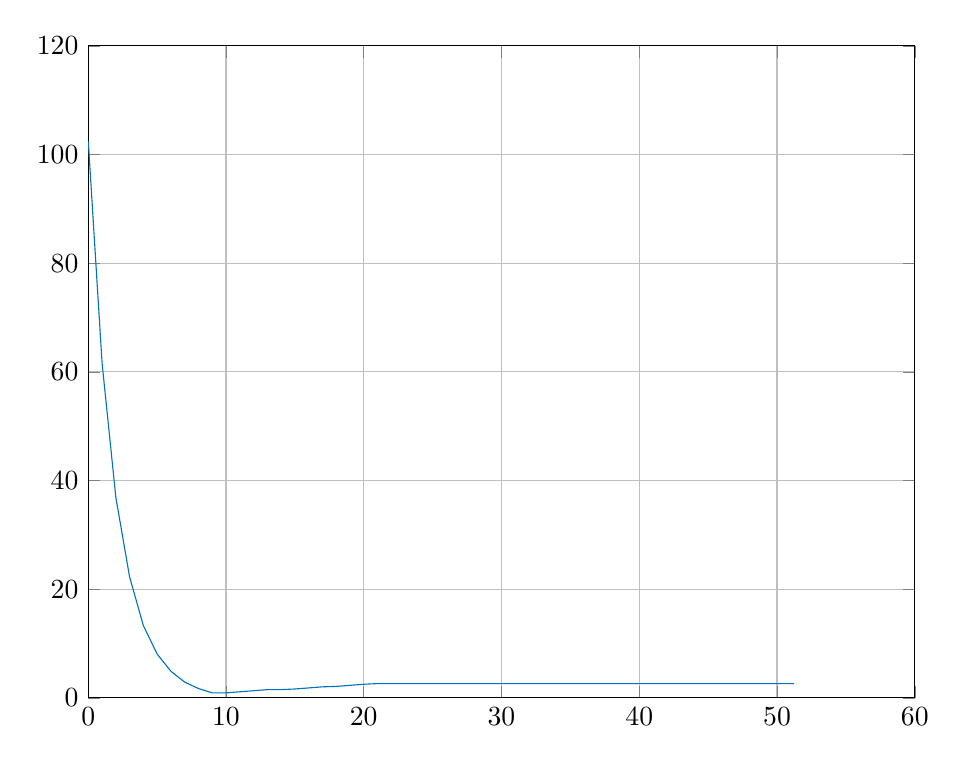
\begin{tikzpicture}

\begin{axis}[%
width=4.133in,
height=3.26in,
at={(0.693in,0.44in)},
scale only axis,
xmin=0,
xmax=60,
xmajorgrids,
ymin=0,
ymax=120,
ymajorgrids,
axis background/.style={fill=white}
]
\addplot [color=mycolor1,solid,forget plot]
  table[row sep=crcr]{%
0	102.4204\\
0.0279184419990005	101.9284\\
0.0366909339990001	101.3644\\
0.0488961359989997	100.7764\\
0.0643262429999998	100.1264\\
0.0799343929989999	99.4924\\
0.0959413429990001	98.8284\\
0.112056496999	98.1844\\
0.127805612	97.5364\\
0.143840067999	96.8924\\
0.159794021999	96.2484\\
0.175811640001	95.5924\\
0.191757119999	94.9404\\
0.207806019999	94.2884\\
0.223890308999	93.6344\\
0.239774361999	92.9564\\
0.255767657999	92.3124\\
0.271812968999	91.6664\\
0.287799526999	91.0204\\
0.303763418000001	90.3664\\
0.319764354	89.6824\\
0.335809329	89.0384\\
0.351793065999	88.3924\\
0.367789345999	87.7484\\
0.383789494	87.1024\\
0.399966247999	86.3184\\
0.415821373	85.7444\\
0.431810161	85.1204\\
0.447762817	84.4684\\
0.463766479999	83.8264\\
0.479853274	83.1804\\
0.495943276	82.5224\\
0.511975914	81.8684\\
0.527979810999	81.2124\\
0.544067607999	80.5604\\
0.559998190999	79.9024\\
0.575944134999	79.2504\\
0.591775071	78.6024\\
0.607750232999	77.9244\\
0.623825626999	77.2804\\
0.639807017999	76.6284\\
0.655871607999	75.9804\\
0.671855088999	75.3304\\
0.687784746	74.6844\\
0.703784847	74.0324\\
0.719922331999	73.3784\\
0.735939949999	72.7244\\
0.751920925	72.0684\\
0.767842861999	71.4164\\
0.783855013	70.7684\\
0.799737443999	70.1184\\
0.827975673001	69.3664\\
0.833377798001	68.7744\\
0.848626284	68.1304\\
0.864296795	67.4784\\
0.879851215	66.7324\\
0.895975453999	66.1604\\
0.912138582999	65.5144\\
0.927863201999	64.8644\\
0.943940986	64.2224\\
0.960087592	63.5764\\
0.975854798001	62.9144\\
0.991877451999	62.2684\\
1.013709321	61.5484\\
1.025515488999	61.1724\\
1.040533303999	60.7984\\
1.055752335	60.4224\\
1.071698581999	60.0344\\
1.087857217	59.6424\\
1.103836052	59.2444\\
1.119811725999	58.8484\\
1.135708780999	58.4544\\
1.151859451	57.9884\\
1.167810052	57.6564\\
1.183832987999	57.2604\\
1.199725815999	56.8544\\
1.216632119999	56.4584\\
1.231806131999	56.0724\\
1.247784595999	55.6824\\
1.263668520999	55.2824\\
1.282015919999	54.8784\\
1.297214722999	54.4864\\
1.312530425999	54.0904\\
1.328005875	53.6984\\
1.343779624999	53.3044\\
1.359835317999	52.9124\\
1.375726640999	52.5024\\
1.391836008999	52.1244\\
1.407822300999	51.7284\\
1.423808006999	51.3284\\
1.439817430999	50.9364\\
1.455820225999	50.5284\\
1.471758479	50.1384\\
1.487818619999	49.7464\\
1.503791411	49.3544\\
1.519728348999	48.9544\\
1.535673133999	48.5604\\
1.553838609999	48.1504\\
1.569345347	47.7564\\
1.584522288999	47.3644\\
1.599805654	46.9724\\
1.615823628	46.5824\\
1.631834631	46.1864\\
1.647784229999	45.7924\\
1.663943263999	45.3944\\
1.679856559	44.9964\\
1.695919302	44.5864\\
1.711799203	44.1924\\
1.727791208	43.8044\\
1.743742045	43.4064\\
1.759755163	43.0164\\
1.775740152999	42.6224\\
1.791774523999	42.2284\\
1.807649571999	41.8344\\
1.826174029	41.4224\\
1.841470943999	41.0284\\
1.856630597999	40.6344\\
1.872260206001	40.2324\\
1.887934748	39.8364\\
1.903920463	39.4544\\
1.919847644999	39.0624\\
1.935734786	38.6684\\
1.951804095999	38.2724\\
1.967805395999	37.8564\\
1.983829057999	37.4804\\
1.999775253999	37.0844\\
2.017467733999	36.7384\\
2.032592568999	36.5184\\
2.047822637	36.2964\\
2.063791064	36.0504\\
2.079745994999	35.8264\\
2.095654237999	35.5964\\
2.111754371	35.3684\\
2.127933399999	35.1304\\
2.143940539999	34.8944\\
2.159978578999	34.6584\\
2.175946249	34.4244\\
2.191762640999	34.1944\\
2.207673173999	33.9484\\
2.223941359999	33.7144\\
2.239779364999	33.4824\\
2.255905849999	33.2504\\
2.271807149999	32.9804\\
2.287687586999	32.7764\\
2.303791320999	32.5424\\
2.319931817	32.3084\\
2.335918860999	32.0804\\
2.351816402	31.8424\\
2.370153076999	31.5984\\
2.385497249	31.3704\\
2.400833376999	31.1324\\
2.416437307999	30.9044\\
2.431899343	30.6704\\
2.448188130999	30.4364\\
2.463923203	30.2004\\
2.479883654	29.9664\\
2.495785137	29.7304\\
2.511839201	29.4924\\
2.527685786999	29.2604\\
2.543759845	29.0284\\
2.559746993999	28.7984\\
2.575774645	28.5504\\
2.59194175	28.3204\\
2.607759588	28.0884\\
2.623773758999	27.8564\\
2.640048585	27.6204\\
2.656152242999	27.3824\\
2.671972102999	27.1464\\
2.687901164999	26.9164\\
2.703824868999	26.6704\\
2.719952503999	26.4384\\
2.7359208	26.2144\\
2.751978234	25.9784\\
2.768080934999	25.7404\\
2.783966092999	25.5084\\
2.799849387	25.2744\\
2.815902909999	25.0284\\
2.831948774	24.8004\\
2.847788970999	24.5664\\
2.863687873	24.3364\\
2.879761335	24.1024\\
2.896000223999	23.8564\\
2.912400509999	23.6244\\
2.927787795	23.3944\\
2.943821047999	23.1544\\
2.959767630999	22.9204\\
2.975811613999	22.6904\\
2.991731179999	22.4564\\
3.012782597	22.2084\\
3.024945338999	22.0704\\
3.040506226999	21.9324\\
3.056075488999	21.7964\\
3.071950979999	21.6404\\
3.088008007999	21.5004\\
3.104084949999	21.3644\\
3.119963838999	21.2164\\
3.135884130999	21.0804\\
3.151879501	20.9384\\
3.167900867	20.7884\\
3.183839229999	20.6444\\
3.199859007999	20.5024\\
3.215814507999	20.3644\\
3.231784965	20.2204\\
3.247773345	20.0724\\
3.263928529999	19.9344\\
3.279844823999	19.7924\\
3.295749489999	19.6424\\
3.311807446	19.5024\\
3.327810230999	19.3624\\
3.343791275999	19.2064\\
3.360111880999	19.0684\\
3.375858644999	18.9244\\
3.391843984999	18.7864\\
3.407856471999	18.6344\\
3.423801817	18.4884\\
3.439696718999	18.3504\\
3.455758951	18.2084\\
3.471866262999	18.0664\\
3.487764437999	17.9264\\
3.503852659	17.7804\\
3.519890412999	17.6384\\
3.535766342999	17.4964\\
3.551742529	17.3524\\
3.567855523999	17.2124\\
3.583831918999	17.0684\\
3.599786564999	16.9144\\
3.615846984999	16.7784\\
3.631771171	16.6324\\
3.64778463	16.4924\\
3.663782383	16.3524\\
3.679667296	16.2104\\
3.695770585999	16.0664\\
3.711818454999	15.9184\\
3.727946804999	15.7744\\
3.743966933999	15.6324\\
3.759736133999	15.4904\\
3.775779172999	15.3484\\
3.791897657	15.2024\\
3.808058385	15.0564\\
3.823778265999	14.9084\\
3.839921099999	14.7724\\
3.855958298001	14.6244\\
3.871847865999	14.4844\\
3.887848480999	14.3444\\
3.903802053999	14.1964\\
3.919798354	14.0544\\
3.935839685999	13.9144\\
3.951875610999	13.7684\\
3.967919795	13.6184\\
3.983958876999	13.4764\\
3.999920142	13.3404\\
4.017600644	13.2224\\
4.033194602	13.1424\\
4.048869357999	13.0624\\
4.064132824	12.9784\\
4.079836682	12.8944\\
4.095835614999	12.8124\\
4.111816477	12.7324\\
4.127826711999	12.6464\\
4.143800235999	12.5624\\
4.159784562999	12.4764\\
4.17574163	12.3944\\
4.191736461	12.3104\\
4.207781151	12.2264\\
4.223662729	12.1444\\
4.241909677	12.0544\\
4.257335223999	11.9684\\
4.272643824999	11.8904\\
4.287788889999	11.8044\\
4.303677635	11.7264\\
4.319766883	11.6384\\
4.335742235	11.5564\\
4.351740788	11.4704\\
4.367945497999	11.3904\\
4.383794989999	11.3044\\
4.399740168999	11.2204\\
4.415877699	11.1384\\
4.432064084999	11.0544\\
4.447672054999	10.9684\\
4.465983111	10.8864\\
4.481042527999	10.7984\\
4.496160281999	10.7144\\
4.511786491999	10.6344\\
4.530058951999	10.5464\\
4.545117505999	10.4644\\
4.560186333999	10.3844\\
4.575874835999	10.2984\\
4.591745772999	10.2164\\
4.607974078	10.1324\\
4.623915939999	10.0484\\
4.639932199999	9.96639999999999\\
4.655919579998	9.88239999999999\\
4.671799195	9.79640000000001\\
4.687639913	9.71239999999997\\
4.703817729	9.63039999999999\\
4.719838710999	9.5444\\
4.735947369999	9.46239999999997\\
4.751969223	9.38039999999999\\
4.767934366999	9.2924\\
4.783820326999	9.20839999999998\\
4.799817112999	9.12639999999999\\
4.815779660999	9.0424\\
4.831783557	8.9584\\
4.847948621	8.87639999999999\\
4.863856805999	8.7944\\
4.879641361999	8.7084\\
4.895789134999	8.6224\\
4.911768806999	8.5424\\
4.927892285999	8.46039999999999\\
4.944081789	8.37439999999999\\
4.959751032999	8.28639999999999\\
4.975667357999	8.2064\\
4.991789029999	8.1224\\
5.013674088999	8.03039999999999\\
5.025547692999	7.98439999999999\\
5.040791567999	7.93640000000001\\
5.056056779999	7.8884\\
5.071718642	7.8364\\
5.088240458999	7.78439999999999\\
5.10387713	7.7324\\
5.119892160999	7.68640000000001\\
5.135940032999	7.63640000000001\\
5.152058343999	7.58240000000001\\
5.167912501999	7.5324\\
5.183955904	7.48439999999999\\
5.199943463999	7.43239999999999\\
5.215814206001	7.3824\\
5.231806815999	7.33240000000001\\
5.247973411999	7.2824\\
5.263937459	7.2304\\
5.279945650999	7.17839999999998\\
5.295941444999	7.12639999999999\\
5.311928192999	7.0784\\
5.327948703	7.0284\\
5.343789861999	6.9744\\
5.359752522999	6.92439999999999\\
5.375882748999	6.87439999999999\\
5.392144830999	6.8224\\
5.407671166	6.7724\\
5.423787508	6.72240000000001\\
5.439946937999	6.67239999999998\\
5.455929721999	6.62039999999999\\
5.472326255	6.57039999999999\\
5.487949048001	6.5184\\
5.503984746999	6.46639999999999\\
5.519927570999	6.41639999999998\\
5.535846029999	6.3664\\
5.551700071999	6.31439999999999\\
5.567778066999	6.2664\\
5.583784670999	6.2144\\
5.599660682	6.16239999999999\\
5.615837166999	6.11239999999999\\
5.63182188	6.06039999999999\\
5.647687704999	6.0124\\
5.664002060999	5.96039999999999\\
5.679908352	5.9104\\
5.696108863999	5.8604\\
5.711801371	5.80639999999998\\
5.727787020998	5.75840000000001\\
5.743688907999	5.7084\\
5.759804763999	5.65639999999999\\
5.775850069999	5.60639999999999\\
5.791774093	5.55439999999999\\
5.807867807	5.50239999999999\\
5.823789352	5.4524\\
5.839653255	5.4024\\
5.855783890999	5.3524\\
5.871784866999	5.30239999999999\\
5.887779863999	5.25039999999998\\
5.903798946	5.19840000000001\\
5.919763408999	5.1504\\
5.935664845999	5.0984\\
5.951754344998	5.04839999999999\\
5.967751350999	4.99839999999999\\
5.983665845999	4.94840000000001\\
5.999788517999	4.8964\\
6.015730161	4.8524\\
6.031862890999	4.82039999999999\\
6.047840089999	4.79039999999999\\
6.063926925	4.7604\\
6.079929037999	4.7304\\
6.096292725999	4.69840000000001\\
6.111838889999	4.66439999999999\\
6.127800255999	4.6324\\
6.143817488999	4.60040000000001\\
6.159766977999	4.57039999999999\\
6.175819649999	4.54039999999999\\
6.191900302	4.50840000000001\\
6.207764436998	4.47839999999999\\
6.223835786999	4.44239999999999\\
6.239793189	4.4084\\
6.255775717999	4.38039999999998\\
6.271779569999	4.35040000000001\\
6.287797072999	4.3184\\
6.303918877998	4.28639999999999\\
6.319776317999	4.25239999999999\\
6.335818771999	4.22040000000001\\
6.351802618999	4.1904\\
6.367779088999	4.1604\\
6.383810869999	4.12839999999998\\
6.399849681	4.09639999999999\\
6.415861789999	4.06239999999998\\
6.431861414999	4.0284\\
6.447789746	3.99839999999999\\
6.463800012	3.9684\\
6.479776951	3.93639999999998\\
6.495785259999	3.9084\\
6.511671423001	3.87039999999999\\
6.5279388	3.8404\\
6.54395501	3.81039999999999\\
6.559954638	3.7804\\
6.575963390999	3.74839999999999\\
6.592059873	3.71239999999999\\
6.607745503999	3.68039999999999\\
6.623797865999	3.6504\\
6.639775619	3.62039999999999\\
6.655761751	3.58840000000001\\
6.671732934	3.55639999999998\\
6.687773984999	3.5224\\
6.703674253	3.48839999999998\\
6.719930992999	3.46039999999999\\
6.735833916999	3.43039999999999\\
6.751863847999	3.3964\\
6.767787387999	3.3664\\
6.783783522999	3.33240000000001\\
6.79978975	3.3004\\
6.816056789	3.2704\\
6.831928204999	3.24039999999999\\
6.847750811998	3.2084\\
6.863893569	3.17639999999999\\
6.879978469998	3.14239999999999\\
6.895811814999	3.1104\\
6.911793031	3.0784\\
6.927780751999	3.04839999999999\\
6.943658227	3.0184\\
6.961936835	2.98639999999999\\
6.977168597	2.9524\\
6.992435699999	2.91839999999999\\
7.013557468999	2.8884\\
7.025465074999	2.87039999999999\\
7.040687586	2.8524\\
7.055956005999	2.83239999999999\\
7.071828940999	2.81439999999998\\
7.087758875999	2.7944\\
7.103946779999	2.7744\\
7.119922473999	2.75639999999999\\
7.135798751999	2.73839999999998\\
7.151799135999	2.72040000000001\\
7.167789722999	2.7024\\
7.183936007999	2.68239999999999\\
7.199962967999	2.66239999999999\\
7.215926281999	2.64239999999999\\
7.231833871	2.62439999999999\\
7.247934286999	2.6044\\
7.263892961999	2.5844\\
7.27993905	2.5684\\
7.295744812999	2.5504\\
7.311817852	2.5284\\
7.327643682999	2.5104\\
7.345896790999	2.49239999999999\\
7.360966902	2.47240000000001\\
7.376039602999	2.4524\\
7.39174992	2.43439999999998\\
7.407795305999	2.41439999999999\\
7.423675758999	2.3964\\
7.441888306999	2.37639999999999\\
7.45594876	2.35839999999999\\
7.471735836999	2.3404\\
7.487771640001	2.32039999999999\\
7.503916531	2.30239999999999\\
7.519993919999	2.2824\\
7.535873621	2.2624\\
7.551791097999	2.24439999999998\\
7.567782217999	2.2244\\
7.583948069999	2.20439999999999\\
7.599930785999	2.18639999999998\\
7.615970383	2.17039999999999\\
7.631879881	2.1504\\
7.647864449999	2.13039999999998\\
7.663812375	2.1104\\
7.679806744999	2.0924\\
7.695812131	2.07239999999999\\
7.71169096	2.05239999999999\\
7.727807838	2.03439999999999\\
7.743947321999	2.01439999999999\\
7.759733569	1.99639999999999\\
7.775803352999	1.97839999999999\\
7.791784147999	1.9584\\
7.80771959	1.9384\\
7.823810493999	1.92039999999999\\
7.83981809	1.9024\\
7.855812720999	1.88239999999999\\
7.871772833999	1.86239999999999\\
7.887809344998	1.84439999999999\\
7.903782692999	1.8244\\
7.919838291999	1.80639999999998\\
7.935954699999	1.7884\\
7.951691925	1.7704\\
7.967807331999	1.75039999999998\\
7.983760343999	1.7304\\
7.999631918999	1.71239999999999\\
8.017604430999	1.69239999999999\\
8.033003546999	1.68239999999999\\
8.048339746	1.6724\\
8.063742104999	1.65639999999999\\
8.079786072999	1.6444\\
8.095685054999	1.63239999999999\\
8.111832109	1.6224\\
8.127816947999	1.60839999999999\\
8.143632890001	1.5924\\
8.159751521999	1.58239999999999\\
8.175777157999	1.5684\\
8.191682557	1.55639999999998\\
8.207781303999	1.5424\\
8.223797218999	1.5324\\
8.239748606999	1.5184\\
8.255832435999	1.50439999999999\\
8.271800029999	1.49239999999999\\
8.287669826	1.4804\\
8.303811402999	1.4684\\
8.319806885999	1.4524\\
8.335692078	1.44239999999999\\
8.351769637999	1.42839999999998\\
8.367946397999	1.41839999999999\\
8.383912277998	1.4024\\
8.399965156999	1.39239999999999\\
8.415947866	1.37839999999998\\
8.431951206999	1.36439999999999\\
8.447869484999	1.3524\\
8.463824574	1.3424\\
8.480276437999	1.3284\\
8.495939763999	1.31439999999998\\
8.511823809999	1.30239999999999\\
8.52779123	1.29039999999999\\
8.543798539999	1.2784\\
8.559775330999	1.2624\\
8.575937963	1.25239999999999\\
8.591948213999	1.23839999999998\\
8.607907795999	1.2264\\
8.623943269	1.21239999999999\\
8.639957053999	1.2024\\
8.656202503999	1.1884\\
8.671798726999	1.17439999999999\\
8.687900170999	1.16239999999999\\
8.703797986999	1.1524\\
8.719745521999	1.1384\\
8.736259890999	1.1224\\
8.751756131999	1.11239999999999\\
8.767933227	1.10040000000001\\
8.78396596	1.08840000000001\\
8.799937703999	1.07239999999999\\
8.815919461	1.06239999999998\\
8.832043074999	1.0504\\
8.848099680999	1.03639999999999\\
8.863988211999	1.02239999999999\\
8.880260131999	1.0124\\
8.895888616	0.99839999999999\\
8.911966289	0.982399999999998\\
8.927963059	0.972400000000007\\
8.943919638999	0.962399999999988\\
8.959798177	0.948400000000007\\
8.975797864999	0.932399999999987\\
8.991777546999	0.922399999999996\\
9.012316202	0.912399999999991\\
9.024231692999	0.910399999999996\\
9.039828958999	0.910399999999996\\
9.055711304999	0.910399999999996\\
9.071804308999	0.910399999999996\\
9.087805671	0.910399999999996\\
9.103777765999	0.910399999999996\\
9.119812503999	0.910399999999996\\
9.135806769	0.910399999999996\\
9.151875788	0.910399999999996\\
9.167941451	0.910399999999996\\
9.183880671999	0.910399999999996\\
9.199817856999	0.910399999999996\\
9.215841484	0.910399999999996\\
9.231850963999	0.910399999999996\\
9.247710585	0.910399999999996\\
9.263860446999	0.910399999999996\\
9.279875935999	0.910399999999996\\
9.295959755	0.910399999999996\\
9.311944407999	0.910399999999996\\
9.327972509999	0.910399999999996\\
9.343916751999	0.910399999999996\\
9.360434247999	0.910399999999996\\
9.375931416999	0.910399999999996\\
9.391954807999	0.910399999999996\\
9.407956626	0.910399999999996\\
9.423813138999	0.910399999999996\\
9.439994954999	0.910399999999996\\
9.45595155	0.910399999999996\\
9.471950616	0.910399999999996\\
9.488274729	0.910399999999996\\
9.503913609	0.910399999999996\\
9.519937465999	0.910399999999996\\
9.535953912	0.910399999999996\\
9.551908351999	0.910399999999996\\
9.567936819999	0.910399999999996\\
9.583915048999	0.910399999999996\\
9.599789286999	0.910399999999996\\
9.615934023999	0.910399999999996\\
9.631801666999	0.910399999999996\\
9.647763675	0.910399999999996\\
9.663741657999	0.910399999999996\\
9.679646347999	0.910399999999996\\
9.695786350999	0.910399999999996\\
9.71185481	0.910399999999996\\
9.727709092999	0.910399999999996\\
9.743988679999	0.910399999999996\\
9.759752046999	0.910399999999996\\
9.775647104999	0.910399999999996\\
9.791944189	0.910399999999996\\
9.808076336999	0.910399999999996\\
9.823745377998	0.910399999999996\\
9.839869696	0.910399999999996\\
9.855959572999	0.910399999999996\\
9.871945668999	0.910399999999996\\
9.887917083	0.910399999999996\\
9.903745938999	0.910399999999996\\
9.919775144	0.910399999999996\\
9.936062627998	0.910399999999996\\
9.951953369	0.910399999999996\\
9.967999877998	0.910399999999996\\
9.983964585999	0.910399999999996\\
9.999967170999	0.910399999999996\\
10.017837241999	0.912399999999991\\
10.033081914	0.914399999999986\\
10.04854734	0.920400000000001\\
10.063770447999	0.920400000000001\\
10.079775102	0.924399999999991\\
10.095776152999	0.930399999999992\\
10.111768994999	0.930399999999992\\
10.127800053999	0.932399999999987\\
10.143801615999	0.940399999999997\\
10.159714671999	0.940399999999997\\
10.175804238999	0.942399999999992\\
10.191807372999	0.950400000000002\\
10.207745225999	0.950400000000002\\
10.223826107999	0.952399999999997\\
10.239770618999	0.958399999999997\\
10.255922132999	0.960399999999993\\
10.271911947999	0.962399999999988\\
10.287936396999	0.966399999999993\\
10.303754116999	0.970399999999998\\
10.319783086	0.972400000000007\\
10.335777126	0.976399999999998\\
10.351723439999	0.980400000000003\\
10.367764574	0.980400000000003\\
10.383740843999	0.984399999999994\\
10.399720032	0.990399999999994\\
10.415782069	0.990399999999994\\
10.431780644	0.992399999999989\\
10.447662944	1.00039999999998\\
10.463761151999	1.00039999999998\\
10.479776339999	1.00239999999999\\
10.495731473	1.0104\\
10.51178024	1.0104\\
10.527772275999	1.0124\\
10.543671545999	1.0204\\
10.559818663	1.0204\\
10.575780098999	1.02239999999999\\
10.591747690999	1.0284\\
10.607946578	1.0304\\
10.624165982999	1.0324\\
10.639843713999	1.03639999999999\\
10.655884767999	1.04039999999999\\
10.671879434	1.04039999999999\\
10.687791611	1.04639999999999\\
10.703922031999	1.0504\\
10.71990409	1.0504\\
10.735906895	1.05439999999999\\
10.752098376999	1.06039999999999\\
10.768167222	1.06039999999999\\
10.783992291	1.0624\\
10.800345232	1.07039999999999\\
10.816635272999	1.07039999999999\\
10.832195323999	1.07239999999999\\
10.847888005999	1.0804\\
10.863818286	1.0804\\
10.879635026	1.08239999999999\\
10.897911701999	1.0904\\
10.913146479	1.0904\\
10.928311623	1.0924\\
10.943805263999	1.0964\\
10.959762685	1.10040000000001\\
10.975956243999	1.1024\\
10.99198231	1.10639999999999\\
11.014310444999	1.1104\\
11.023874156	1.11239999999999\\
11.039863737	1.11439999999999\\
11.055754322999	1.12039999999999\\
11.071741584	1.12039999999999\\
11.087961704	1.12439999999999\\
11.104060361	1.13039999999998\\
11.119860891999	1.13039999999998\\
11.135921061998	1.13239999999999\\
11.151944573999	1.1404\\
11.167984296999	1.1404\\
11.183871113999	1.14239999999999\\
11.199949449999	1.1504\\
11.215768463	1.1504\\
11.231761449999	1.1524\\
11.247737318999	1.1584\\
11.263621258999	1.1604\\
11.279918425999	1.16239999999999\\
11.295973148999	1.1664\\
11.311782003999	1.1704\\
11.327777531999	1.1704\\
11.343936972	1.17639999999999\\
11.359945248999	1.18039999999999\\
11.376389118999	1.18039999999999\\
11.392147072999	1.18440000000001\\
11.408044608999	1.1904\\
11.423827416	1.1904\\
11.440213981999	1.19239999999999\\
11.458762323999	1.2004\\
11.472083831999	1.2004\\
11.488168251999	1.2024\\
11.503941786999	1.21039999999999\\
11.519821015999	1.21039999999999\\
11.535810490999	1.21239999999999\\
11.551698888999	1.2184\\
11.567751574	1.2204\\
11.583762296999	1.22240000000001\\
11.599675879999	1.2264\\
11.617902427	1.2304\\
11.633259740999	1.2324\\
11.648661828999	1.23639999999999\\
11.664148889999	1.24039999999999\\
11.679955625	1.24039999999999\\
11.695813306999	1.24439999999998\\
11.711843223	1.25039999999998\\
11.727790530999	1.25039999999998\\
11.743909975	1.25439999999999\\
11.759921821	1.2604\\
11.775802668999	1.2604\\
11.791654050999	1.2624\\
11.807747375999	1.2704\\
11.823746196	1.2704\\
11.839647135999	1.27239999999999\\
11.857774940999	1.2804\\
11.872740549999	1.2804\\
11.888073536999	1.2824\\
11.903938644	1.2884\\
11.92009188	1.29039999999999\\
11.936043929999	1.29239999999999\\
11.952149899	1.29639999999999\\
11.968075878999	1.3004\\
11.983774752998	1.3004\\
11.999948301999	1.30639999999998\\
12.017566895998	1.31039999999999\\
12.033466904999	1.31039999999999\\
12.048065978999	1.31440000000001\\
12.063759427999	1.32039999999999\\
12.079742347	1.32039999999999\\
12.095817821	1.32239999999999\\
12.11181134	1.3304\\
12.127726309999	1.3304\\
12.143887394	1.33239999999999\\
12.159734841999	1.3404\\
12.175665637999	1.3404\\
12.191738291	1.3424\\
12.207751149	1.3484\\
12.223650223999	1.35040000000001\\
12.239738206001	1.3524\\
12.255776892	1.35839999999999\\
12.271672100999	1.3604\\
12.287790013999	1.3604\\
12.303834708999	1.36639999999998\\
12.319690218999	1.37039999999999\\
12.335794814999	1.37039999999999\\
12.351805904	1.37639999999999\\
12.367792612	1.38039999999998\\
12.383867930999	1.38039999999998\\
12.399930571	1.38439999999999\\
12.415783005	1.3904\\
12.431754097999	1.3904\\
12.447733505999	1.39239999999999\\
12.463862805999	1.4004\\
12.479858787	1.4004\\
12.495873404999	1.4024\\
12.511820500999	1.4104\\
12.527938646999	1.4104\\
12.543963218999	1.41239999999999\\
12.559955617	1.41839999999999\\
12.576097562	1.4204\\
12.591950526999	1.4224\\
12.607752600999	1.42639999999999\\
12.623804663	1.43039999999999\\
12.639724381999	1.43039999999999\\
12.65569188	1.43440000000001\\
12.671804838999	1.4404\\
12.687789396999	1.4404\\
12.703714857999	1.4444\\
12.720072315	1.4504\\
12.735872685999	1.4504\\
12.751916262999	1.4524\\
12.768042258	1.46039999999999\\
12.783960815999	1.46039999999999\\
12.799966637999	1.46239999999999\\
12.815956647999	1.4704\\
12.832160899999	1.4704\\
12.847789989999	1.47240000000001\\
12.863848954	1.47839999999999\\
12.880135441999	1.4804\\
12.895747557	1.4824\\
12.911971036999	1.48639999999999\\
12.927907369999	1.49039999999999\\
12.943816284	1.49239999999999\\
12.959987573999	1.49639999999998\\
12.975941508	1.50039999999998\\
12.991972381	1.50039999999998\\
13.016139319999	1.50239999999999\\
13.024867326999	1.50439999999999\\
13.040227368999	1.50439999999999\\
13.056110883999	1.50439999999999\\
13.071907571	1.50439999999999\\
13.087800271999	1.50439999999999\\
13.103775619	1.50439999999999\\
13.119890071999	1.50439999999999\\
13.135668559	1.50439999999999\\
13.151923258999	1.50439999999999\\
13.167802628999	1.50439999999999\\
13.183681914	1.50439999999999\\
13.199816501999	1.50439999999999\\
13.215934793999	1.50439999999999\\
13.231912671999	1.50439999999999\\
13.247938758999	1.50439999999999\\
13.263977425999	1.50439999999999\\
13.279945937999	1.50439999999999\\
13.295785010999	1.50439999999999\\
13.312070597	1.50439999999999\\
13.327939598	1.50439999999999\\
13.343975137999	1.50439999999999\\
13.360059125999	1.50439999999999\\
13.376127724999	1.50439999999999\\
13.391946387	1.50439999999999\\
13.407951713	1.50439999999999\\
13.423776998	1.50439999999999\\
13.439963977	1.50439999999999\\
13.455909787999	1.50439999999999\\
13.472085258999	1.50439999999999\\
13.487916279	1.50439999999999\\
13.503766788999	1.50439999999999\\
13.519651611999	1.50439999999999\\
13.535768585	1.50439999999999\\
13.551852177999	1.50439999999999\\
13.567941357999	1.50439999999999\\
13.583756111999	1.50439999999999\\
13.599818651999	1.50439999999999\\
13.615770708999	1.50439999999999\\
13.631930347	1.50439999999999\\
13.647756140001	1.50439999999999\\
13.663782183	1.50439999999999\\
13.679971204999	1.50439999999999\\
13.695972947	1.50439999999999\\
13.711832737	1.50439999999999\\
13.727955598999	1.50439999999999\\
13.743939460999	1.50439999999999\\
13.759943418999	1.50439999999999\\
13.775965121	1.50439999999999\\
13.791947279	1.50439999999999\\
13.807927411999	1.50439999999999\\
13.823955846	1.50439999999999\\
13.839940267999	1.50439999999999\\
13.856002904	1.50439999999999\\
13.871951565999	1.50439999999999\\
13.887896508999	1.50439999999999\\
13.903667934999	1.50439999999999\\
13.919766526999	1.50439999999999\\
13.935807633	1.50439999999999\\
13.951688206001	1.50439999999999\\
13.967810717	1.50439999999999\\
13.983799404999	1.50439999999999\\
13.999688413999	1.50439999999999\\
14.017467828	1.50839999999999\\
14.032610758999	1.50839999999999\\
14.048090538	1.50839999999999\\
14.063838956001	1.51239999999999\\
14.079915397999	1.51439999999999\\
14.095972213999	1.51439999999999\\
14.111965438	1.5184\\
14.127941512	1.5204\\
14.143834893999	1.5204\\
14.159877098	1.52439999999999\\
14.175972381999	1.5264\\
14.191984472999	1.5264\\
14.207913214999	1.52839999999999\\
14.223937138999	1.53239999999998\\
14.23999605	1.53239999999998\\
14.256007899999	1.53439999999998\\
14.272572001999	1.53839999999998\\
14.288087020999	1.53839999999998\\
14.303940797999	1.54040000000001\\
14.319945281	1.5444\\
14.335937583	1.5444\\
14.351969533999	1.54639999999999\\
14.367954832999	1.5504\\
14.383826065	1.5504\\
14.399817804999	1.5504\\
14.415923713	1.5544\\
14.431848241	1.5564\\
14.447812011999	1.5564\\
14.463757555999	1.56039999999999\\
14.479849453	1.5624\\
14.495944912999	1.5624\\
14.511835382999	1.56439999999999\\
14.527897592999	1.56839999999998\\
14.543790944	1.56839999999998\\
14.559793022999	1.57039999999998\\
14.575822266999	1.5744\\
14.591845081999	1.5744\\
14.607834371	1.57639999999999\\
14.623676381999	1.58039999999998\\
14.639854072999	1.58039999999998\\
14.655881913999	1.58239999999998\\
14.671734126999	1.5864\\
14.687804796	1.5864\\
14.703816746999	1.5864\\
14.719842719998	1.5924\\
14.736075293999	1.5924\\
14.751858410999	1.5924\\
14.767699248999	1.59639999999999\\
14.783837720999	1.5984\\
14.799810226999	1.5984\\
14.815656571	1.60239999999999\\
14.831824927	1.60439999999998\\
14.847849054999	1.60439999999998\\
14.863731584999	1.60839999999999\\
14.879884978999	1.61039999999998\\
14.895882717999	1.61039999999998\\
14.911751090999	1.61239999999998\\
14.927788974999	1.61639999999997\\
14.946393006999	1.61639999999997\\
14.961534625	1.61839999999999\\
14.976901934999	1.6224\\
14.992163192999	1.6224\\
15.016163093	1.62440000000001\\
15.024885121	1.63039999999999\\
15.040126975999	1.63039999999999\\
15.055788939999	1.63039999999999\\
15.071809472999	1.63839999999999\\
15.087785001999	1.64039999999999\\
15.103748916999	1.64039999999999\\
15.119827309	1.6484\\
15.135783512999	1.65039999999999\\
15.151707352999	1.65039999999999\\
15.167798062999	1.6584\\
15.183796927999	1.6604\\
15.199702126999	1.6604\\
15.215836489999	1.66439999999999\\
15.23182425	1.6704\\
15.247633239999	1.6704\\
15.263958566999	1.67439999999999\\
15.279949666999	1.68039999999999\\
15.296168227999	1.68039999999999\\
15.311792736	1.6824\\
15.32781706	1.69039999999998\\
15.343856443999	1.69039999999998\\
15.359747793999	1.69039999999998\\
15.375943092	1.69839999999999\\
15.391919174999	1.70039999999999\\
15.407868517999	1.70039999999999\\
15.423785854	1.70840000000001\\
15.439725618999	1.71040000000001\\
15.455866925	1.71040000000001\\
15.471962644999	1.7184\\
15.487927399	1.7204\\
15.503944575999	1.7204\\
15.520056357999	1.72439999999999\\
15.535808083999	1.73039999999999\\
15.551765855999	1.73039999999999\\
15.568102562	1.73439999999998\\
15.583762409999	1.74039999999999\\
15.599827630999	1.74039999999999\\
15.615866437	1.74239999999999\\
15.631667965999	1.75039999999998\\
15.647805811998	1.75039999999998\\
15.663862779	1.75039999999998\\
15.679838427	1.76039999999999\\
15.695919835	1.76039999999999\\
15.711986314999	1.76039999999999\\
15.727849106999	1.7684\\
15.743744277999	1.7704\\
15.760100267999	1.7704\\
15.775791640999	1.7784\\
15.791929237	1.7804\\
15.807928454	1.7804\\
15.823946161999	1.7884\\
15.840132092	1.79040000000001\\
15.855862419	1.79040000000001\\
15.871672130999	1.7944\\
15.887781097	1.8004\\
15.903847003999	1.8004\\
15.919749706999	1.80239999999999\\
15.935940423001	1.81039999999999\\
15.952000241999	1.81039999999999\\
15.967765589	1.8124\\
15.983941364999	1.82039999999999\\
16.00015121	1.82039999999999\\
16.017659921999	1.82239999999999\\
16.032992798999	1.83039999999998\\
16.048129921998	1.83039999999998\\
16.063752710999	1.83039999999998\\
16.079849456999	1.83840000000001\\
16.095809705999	1.8404\\
16.111668007999	1.8404\\
16.127821884999	1.8484\\
16.143810493	1.85039999999999\\
16.159821154999	1.85039999999999\\
16.175814338	1.85439999999998\\
16.191818503	1.86039999999998\\
16.207674432999	1.86039999999998\\
16.223968427999	1.86239999999998\\
16.240074972	1.87039999999999\\
16.255864524	1.87039999999999\\
16.271888236	1.8724\\
16.288074782	1.88039999999999\\
16.303869595999	1.88039999999999\\
16.319953409	1.88039999999999\\
16.335819303	1.89039999999999\\
16.351695876999	1.89039999999999\\
16.367875802999	1.89039999999999\\
16.383805232	1.8984\\
16.399671366	1.90039999999999\\
16.415786029999	1.90039999999999\\
16.431795334999	1.9084\\
16.447937199999	1.9104\\
16.463905595999	1.9104\\
16.479825402999	1.91639999999998\\
16.495988911999	1.9204\\
16.511884222999	1.9204\\
16.528066749999	1.92439999999999\\
16.543893151	1.93039999999999\\
16.559899909	1.93039999999999\\
16.575922713999	1.9324\\
16.591811986	1.94039999999998\\
16.607797998999	1.94039999999998\\
16.623860036999	1.94239999999999\\
16.639889517	1.95039999999999\\
16.655843879999	1.95039999999999\\
16.671823597999	1.95039999999999\\
16.690592809	1.96040000000001\\
16.703876365999	1.96040000000001\\
16.719759902999	1.96040000000001\\
16.73592597	1.9684\\
16.751843711999	1.9704\\
16.767905527999	1.9704\\
16.783718449999	1.97839999999999\\
16.799723371999	1.98039999999999\\
16.815774047999	1.98039999999999\\
16.831683626999	1.98439999999998\\
16.847727350999	1.99039999999999\\
16.863718414	1.99039999999999\\
16.879692836999	1.99439999999998\\
16.895820514999	2.00039999999998\\
16.911759211999	2.00039999999998\\
16.927705223999	2.00239999999999\\
16.943889470999	2.01039999999999\\
16.959860559	2.01039999999999\\
16.975920012	2.01039999999999\\
16.991982376999	2.0204\\
17.013429486	2.0204\\
17.025349517	2.0204\\
17.040652305999	2.02439999999999\\
17.056100001999	2.02439999999999\\
17.071786009999	2.02439999999999\\
17.087921619999	2.0284\\
17.103926473999	2.0284\\
17.119930952999	2.0284\\
17.135889446999	2.0324\\
17.151858895999	2.0324\\
17.167953272999	2.0324\\
17.183955491999	2.03439999999999\\
17.199856951999	2.03639999999999\\
17.215705847999	2.03639999999999\\
17.231931427	2.03639999999999\\
17.247814814999	2.04039999999999\\
17.263763034999	2.04039999999999\\
17.279856737999	2.04039999999999\\
17.295842182	2.04439999999998\\
17.311862512999	2.04439999999998\\
17.327962604	2.04439999999998\\
17.343846328	2.0484\\
17.359939622999	2.0484\\
17.376130324	2.0484\\
17.391988791	2.05240000000001\\
17.407900607999	2.05240000000001\\
17.423837826	2.05240000000001\\
17.439749470999	2.0564\\
17.455786807	2.0564\\
17.471784199999	2.0564\\
17.487752475999	2.05839999999999\\
17.503667571999	2.06039999999999\\
17.519778576999	2.06039999999999\\
17.535878852999	2.0624\\
17.551821154999	2.06439999999999\\
17.567823619999	2.06439999999999\\
17.583797628999	2.06439999999999\\
17.599811814	2.06839999999998\\
17.615889298999	2.06839999999998\\
17.631815193999	2.06839999999998\\
17.647743218999	2.07239999999999\\
17.663818838999	2.07239999999999\\
17.679778269999	2.07239999999999\\
17.695735476999	2.07639999999999\\
17.711815762	2.07639999999999\\
17.727907678998	2.07639999999999\\
17.743749413	2.0804\\
17.760061057999	2.0804\\
17.775981847	2.0804\\
17.791774770999	2.08439999999999\\
17.808072629	2.08439999999999\\
17.823917637	2.08439999999999\\
17.840006472	2.0864\\
17.856043163	2.08839999999999\\
17.871924407	2.08839999999999\\
17.888058171	2.08839999999999\\
17.9039358	2.09239999999998\\
17.919983315999	2.09239999999998\\
17.935944771999	2.09239999999998\\
17.951912913	2.0964\\
17.967868429999	2.0964\\
17.983930800999	2.0964\\
17.999962034999	2.10040000000001\\
18.017970514999	2.10040000000001\\
18.033474152999	2.1024\\
18.049007899999	2.1104\\
18.064370042999	2.1104\\
18.079945498999	2.1104\\
18.095785068999	2.12039999999999\\
18.111943430999	2.12039999999999\\
18.127965234	2.12039999999999\\
18.143809925	2.13039999999998\\
18.159758729999	2.13039999999998\\
18.175777633999	2.13039999999998\\
18.191746357	2.1384\\
18.207930376999	2.1404\\
18.223771163999	2.1404\\
18.239967277999	2.14439999999999\\
18.255992202	2.1504\\
18.272075078999	2.1504\\
18.287936848999	2.1544\\
18.304060922999	2.1604\\
18.319975397999	2.1604\\
18.336076469998	2.16239999999999\\
18.352080833	2.1704\\
18.367747220999	2.1704\\
18.383941338999	2.1704\\
18.400161375999	2.18039999999999\\
18.415889021999	2.18039999999999\\
18.431917033999	2.18039999999999\\
18.447933339	2.1904\\
18.463978890999	2.1904\\
18.479730771999	2.1904\\
18.495888854	2.19840000000001\\
18.511842175999	2.2004\\
18.527770973999	2.2004\\
18.543783509999	2.20439999999999\\
18.559812689999	2.21039999999999\\
18.575951868999	2.21039999999999\\
18.591924079	2.21439999999998\\
18.607965851999	2.2204\\
18.625726746999	2.2204\\
18.641219239999	2.2244\\
18.656725088	2.2304\\
18.672314916999	2.2304\\
18.687909687	2.2324\\
18.703802737999	2.24039999999999\\
18.719761406999	2.24039999999999\\
18.735984541999	2.24039999999999\\
18.752005321999	2.25039999999998\\
18.767795098999	2.25039999999998\\
18.783844248999	2.25039999999998\\
18.799816756	2.25840000000001\\
18.815918249	2.2604\\
18.832092065999	2.2604\\
18.847864159999	2.2684\\
18.863924196999	2.2704\\
18.879908790999	2.2704\\
18.895775020999	2.27439999999999\\
18.911836593999	2.2804\\
18.927791649999	2.2804\\
18.943672179999	2.2824\\
18.961998644	2.29039999999999\\
18.977083688999	2.29039999999999\\
18.992145781999	2.29239999999999\\
19.013211771999	2.3004\\
19.025006459	2.3004\\
19.040136394999	2.30239999999999\\
19.055893432999	2.31039999999999\\
19.071818691999	2.31039999999999\\
19.087669335999	2.31039999999999\\
19.103781579998	2.32039999999999\\
19.119769736	2.32039999999999\\
19.135763740999	2.32039999999999\\
19.154274715	2.3284\\
19.169757701999	2.3304\\
19.185139057999	2.3304\\
19.200445193999	2.3364\\
19.215845743999	2.3404\\
19.231956938999	2.3404\\
19.247938526	2.34440000000001\\
19.263948291999	2.35040000000001\\
19.279954929999	2.35040000000001\\
19.295947406	2.3524\\
19.31190551	2.3604\\
19.327885873999	2.3604\\
19.343868842999	2.36239999999999\\
19.359868721999	2.37039999999999\\
19.375774475999	2.37039999999999\\
19.391947305999	2.37039999999999\\
19.407954650999	2.38039999999998\\
19.423951979	2.38039999999998\\
19.439949676999	2.38039999999998\\
19.456082746999	2.3904\\
19.471936839999	2.3904\\
19.487767498999	2.3904\\
19.503785638999	2.39840000000001\\
19.519811866999	2.4004\\
19.535788681999	2.4004\\
19.551997017999	2.4044\\
19.567947543999	2.4104\\
19.584127255	2.4104\\
19.599910376999	2.41439999999999\\
19.615874038999	2.4204\\
19.631850467999	2.4204\\
19.647785003	2.4224\\
19.663954531	2.43039999999999\\
19.679944470999	2.43039999999999\\
19.695870216	2.43039999999999\\
19.711837913999	2.4404\\
19.72792205	2.4404\\
19.743867760999	2.4404\\
19.760064216999	2.4504\\
19.775824208999	2.4504\\
19.791769708999	2.4504\\
19.807773424999	2.4584\\
19.823937390001	2.46039999999999\\
19.839832015001	2.46039999999999\\
19.856067932999	2.46639999999999\\
19.871958147999	2.4704\\
19.887799039999	2.4704\\
19.903782355999	2.4744\\
19.919777368	2.4804\\
19.935790240999	2.4804\\
19.951929104	2.4824\\
19.967968686998	2.49039999999999\\
19.983796625	2.49039999999999\\
19.999676005	2.49239999999999\\
20.017716613999	2.49839999999999\\
20.032824189999	2.49839999999999\\
20.047931053	2.49839999999999\\
20.063908119999	2.50439999999999\\
20.079753652999	2.50439999999999\\
20.095923646999	2.50439999999999\\
20.112069480999	2.51039999999999\\
20.128050189999	2.51039999999999\\
20.143720092999	2.51039999999999\\
20.159913015999	2.5164\\
20.175946576	2.5164\\
20.191923697	2.5164\\
20.207823539	2.5204\\
20.223803646999	2.52239999999999\\
20.239778884999	2.52239999999999\\
20.255915922999	2.5264\\
20.271774811998	2.52839999999999\\
20.287794395	2.52839999999999\\
20.303921079999	2.53039999999999\\
20.320058925999	2.53439999999998\\
20.33595102	2.53439999999998\\
20.351917271999	2.53439999999998\\
20.367962713	2.54039999999999\\
20.383796625	2.54039999999999\\
20.399876914999	2.54039999999999\\
20.415788083	2.54639999999999\\
20.431788381	2.54639999999999\\
20.447744800999	2.54639999999999\\
20.463936152999	2.55239999999999\\
20.479949160999	2.55239999999999\\
20.495947781999	2.55239999999999\\
20.512178588	2.55839999999999\\
20.527927792999	2.55839999999999\\
20.543943121	2.55839999999999\\
20.559922321999	2.5624\\
20.575800719998	2.56439999999999\\
20.591746319999	2.56439999999999\\
20.607799723999	2.56639999999999\\
20.623668558999	2.57039999999999\\
20.640051050999	2.57039999999999\\
20.655977036999	2.57239999999999\\
20.671915405999	2.57639999999999\\
20.687921777999	2.57639999999999\\
20.703868576	2.57639999999999\\
20.719752788999	2.58239999999999\\
20.735971871999	2.58239999999999\\
20.752102727	2.58239999999999\\
20.767682309999	2.58839999999999\\
20.783788663	2.58839999999999\\
20.799917588	2.58839999999999\\
20.815975160999	2.59439999999999\\
20.831937463999	2.59439999999999\\
20.848149146999	2.59439999999999\\
20.863864164999	2.5984\\
20.879938290999	2.60039999999999\\
20.895948788999	2.60039999999999\\
20.911891857999	2.60439999999998\\
20.927752385	2.60639999999998\\
20.943765894	2.60639999999998\\
20.959796165999	2.60839999999999\\
20.975909530999	2.61239999999998\\
20.991761989999	2.61239999999998\\
21.012623803	2.61239999999998\\
21.024711378999	2.61239999999998\\
21.040056371999	2.61239999999998\\
21.055776265999	2.61239999999998\\
21.071852607999	2.61239999999998\\
21.087781975999	2.61239999999998\\
21.103815911999	2.61239999999998\\
21.119814561998	2.61239999999998\\
21.135817491999	2.61239999999998\\
21.151786409999	2.61239999999998\\
21.167788293	2.61239999999998\\
21.183795015999	2.61239999999998\\
21.199778156	2.61239999999998\\
21.215806078	2.61239999999998\\
21.231863480999	2.61239999999998\\
21.247784005	2.61239999999998\\
21.263779156999	2.61239999999998\\
21.279804336999	2.61239999999998\\
21.295780592	2.61239999999998\\
21.311791013999	2.61239999999998\\
21.327772379999	2.61239999999998\\
21.343778627998	2.61239999999998\\
21.359760295	2.61239999999998\\
21.375948223999	2.61239999999998\\
21.391940845999	2.61239999999998\\
21.408065406	2.61239999999998\\
21.423850919	2.61239999999998\\
21.440049326	2.61239999999998\\
21.455970686998	2.61239999999998\\
21.471880395999	2.61239999999998\\
21.487776119999	2.61239999999998\\
21.504052476999	2.61239999999998\\
21.519803456001	2.61239999999998\\
21.535789908999	2.61239999999998\\
21.551782750999	2.61239999999998\\
21.567829836	2.61239999999998\\
21.583860397999	2.61239999999998\\
21.599890560999	2.61239999999998\\
21.616046562999	2.61239999999998\\
21.631877901999	2.61239999999998\\
21.647751023999	2.61239999999998\\
21.663791324999	2.61239999999998\\
21.679676700999	2.61239999999998\\
21.695781413999	2.61239999999998\\
21.711860255999	2.61239999999998\\
21.727919133	2.61239999999998\\
21.743969279999	2.61239999999998\\
21.759857524999	2.61239999999998\\
21.775711852999	2.61239999999998\\
21.791949740999	2.61239999999998\\
21.807822399999	2.61239999999998\\
21.823765284	2.61239999999998\\
21.839775410999	2.61239999999998\\
21.855939986999	2.61239999999998\\
21.87194192	2.61239999999998\\
21.887910312	2.61239999999998\\
21.903783391999	2.61239999999998\\
21.919967577999	2.61239999999998\\
21.935952387	2.61239999999998\\
21.951958814999	2.61239999999998\\
21.967913830999	2.61239999999998\\
21.983947430999	2.61239999999998\\
22.000004302999	2.61239999999998\\
22.017543845999	2.61239999999998\\
22.032669718	2.61239999999998\\
22.047997988999	2.61239999999998\\
22.063885022999	2.61239999999998\\
22.079964489999	2.61239999999998\\
22.095764215	2.61239999999998\\
22.111763576999	2.61239999999998\\
22.127905993	2.61239999999998\\
22.143794093	2.61239999999998\\
22.159803704999	2.61239999999998\\
22.175779350999	2.61239999999998\\
22.191824836999	2.61239999999998\\
22.207808628999	2.61239999999998\\
22.223920902	2.61239999999998\\
22.240152175	2.61239999999998\\
22.255766175	2.61239999999998\\
22.272059671998	2.61239999999998\\
22.288087046999	2.61239999999998\\
22.303925678999	2.61239999999998\\
22.319755572999	2.61239999999998\\
22.335735996	2.61239999999998\\
22.351791661	2.61239999999998\\
22.367776970999	2.61239999999998\\
22.383809668999	2.61239999999998\\
22.399776215999	2.61239999999998\\
22.415780003	2.61239999999998\\
22.431777847	2.61239999999998\\
22.447786173999	2.61239999999998\\
22.463814300999	2.61239999999998\\
22.479827479999	2.61239999999998\\
22.495759666999	2.61239999999998\\
22.511941109	2.61239999999998\\
22.527949887	2.61239999999998\\
22.543844280999	2.61239999999998\\
22.559937415999	2.61239999999998\\
22.575962304999	2.61239999999998\\
22.592161484999	2.61239999999998\\
22.607938211999	2.61239999999998\\
22.623823606999	2.61239999999998\\
22.639815269999	2.61239999999998\\
22.655917119999	2.61239999999998\\
22.671804973999	2.61239999999998\\
22.687701597	2.61239999999998\\
22.703937646999	2.61239999999998\\
22.720067855	2.61239999999998\\
22.735921387	2.61239999999998\\
22.751763631999	2.61239999999998\\
22.767967934	2.61239999999998\\
22.783985932999	2.61239999999998\\
22.799769451	2.61239999999998\\
22.815904741	2.61239999999998\\
22.832317238999	2.61239999999998\\
22.847807030999	2.61239999999998\\
22.863788115999	2.61239999999998\\
22.880100026999	2.61239999999998\\
22.895934604999	2.61239999999998\\
22.911823703	2.61239999999998\\
22.927817055999	2.61239999999998\\
22.943744644999	2.61239999999998\\
22.959782067999	2.61239999999998\\
22.975706477999	2.61239999999998\\
22.991906105999	2.61239999999998\\
23.012715399999	2.61239999999998\\
23.024679034999	2.61239999999998\\
23.040006534	2.61239999999998\\
23.055843737999	2.61239999999998\\
23.071759865999	2.61239999999998\\
23.087744133999	2.61239999999998\\
23.103733247999	2.61239999999998\\
23.119652552	2.61239999999998\\
23.135817926999	2.61239999999998\\
23.151796651999	2.61239999999998\\
23.167839732999	2.61239999999998\\
23.183936555999	2.61239999999998\\
23.199940738999	2.61239999999998\\
23.215883321999	2.61239999999998\\
23.231931619999	2.61239999999998\\
23.247958444	2.61239999999998\\
23.263916000999	2.61239999999998\\
23.279927284999	2.61239999999998\\
23.295925283999	2.61239999999998\\
23.311945618	2.61239999999998\\
23.328389934	2.61239999999998\\
23.343922016999	2.61239999999998\\
23.359910949	2.61239999999998\\
23.376151308	2.61239999999998\\
23.391860277	2.61239999999998\\
23.407648901	2.61239999999998\\
23.425908276	2.61239999999998\\
23.441000371	2.61239999999998\\
23.456244426	2.61239999999998\\
23.471945617999	2.61239999999998\\
23.487914349999	2.61239999999998\\
23.503942897999	2.61239999999998\\
23.519873994999	2.61239999999998\\
23.536065427	2.61239999999998\\
23.551847220999	2.61239999999998\\
23.567966594998	2.61239999999998\\
23.583943039999	2.61239999999998\\
23.599919038999	2.61239999999998\\
23.615937940999	2.61239999999998\\
23.631895908999	2.61239999999998\\
23.647960488999	2.61239999999998\\
23.663998578	2.61239999999998\\
23.679926407999	2.61239999999998\\
23.695937861999	2.61239999999998\\
23.711880640999	2.61239999999998\\
23.727935954999	2.61239999999998\\
23.744265364999	2.61239999999998\\
23.759776880999	2.61239999999998\\
23.775920324999	2.61239999999998\\
23.791809736999	2.61239999999998\\
23.807842900999	2.61239999999998\\
23.823798419	2.61239999999998\\
23.839775091	2.61239999999998\\
23.855947303	2.61239999999998\\
23.872084852999	2.61239999999998\\
23.887713313	2.61239999999998\\
23.903792180999	2.61239999999998\\
23.919930843999	2.61239999999998\\
23.935944718999	2.61239999999998\\
23.951955136	2.61239999999998\\
23.967933544999	2.61239999999998\\
23.983769157999	2.61239999999998\\
23.999927432999	2.61239999999998\\
24.017447998	2.61239999999998\\
24.032684390999	2.61239999999998\\
24.047795949999	2.61239999999998\\
24.063790976999	2.61239999999998\\
24.07981725	2.61239999999998\\
24.095802526	2.61239999999998\\
24.111773944	2.61239999999998\\
24.127789392999	2.61239999999998\\
24.143831406	2.61239999999998\\
24.159784958999	2.61239999999998\\
24.175770607999	2.61239999999998\\
24.191913772999	2.61239999999998\\
24.207918666999	2.61239999999998\\
24.223692015001	2.61239999999998\\
24.239780951999	2.61239999999998\\
24.255942310999	2.61239999999998\\
24.271797762	2.61239999999998\\
24.287773730999	2.61239999999998\\
24.303778314999	2.61239999999998\\
24.322070677999	2.61239999999998\\
24.337158715	2.61239999999998\\
24.352369955999	2.61239999999998\\
24.367769723999	2.61239999999998\\
24.383783157	2.61239999999998\\
24.399939790999	2.61239999999998\\
24.415981974999	2.61239999999998\\
24.432096187	2.61239999999998\\
24.448139925	2.61239999999998\\
24.463780927	2.61239999999998\\
24.479947489999	2.61239999999998\\
24.495984463	2.61239999999998\\
24.511923246999	2.61239999999998\\
24.527808986	2.61239999999998\\
24.543931402999	2.61239999999998\\
24.559934497999	2.61239999999998\\
24.575940164	2.61239999999998\\
24.591924201	2.61239999999998\\
24.607933364999	2.61239999999998\\
24.623769005999	2.61239999999998\\
24.639782805999	2.61239999999998\\
24.655914822999	2.61239999999998\\
24.671873529	2.61239999999998\\
24.687771881999	2.61239999999998\\
24.703782107999	2.61239999999998\\
24.719941582999	2.61239999999998\\
24.735944137	2.61239999999998\\
24.751784904999	2.61239999999998\\
24.767786270999	2.61239999999998\\
24.783760976999	2.61239999999998\\
24.79999444	2.61239999999998\\
24.815779690999	2.61239999999998\\
24.83177772	2.61239999999998\\
24.847909532	2.61239999999998\\
24.863922519999	2.61239999999998\\
24.879791762	2.61239999999998\\
24.895791514999	2.61239999999998\\
24.911914562	2.61239999999998\\
24.927892700999	2.61239999999998\\
24.943779538	2.61239999999998\\
24.959793894	2.61239999999998\\
24.975849437999	2.61239999999998\\
24.991671036999	2.61239999999998\\
25.012409163999	2.61239999999998\\
25.024310758999	2.61239999999998\\
25.039702802999	2.61239999999998\\
25.055810326999	2.61239999999998\\
25.071774874	2.61239999999998\\
25.087832798999	2.61239999999998\\
25.103784428	2.61239999999998\\
25.119794183999	2.61239999999998\\
25.135763396999	2.61239999999998\\
25.15174125	2.61239999999998\\
25.167751737999	2.61239999999998\\
25.183673267999	2.61239999999998\\
25.199802960999	2.61239999999998\\
25.215832665999	2.61239999999998\\
25.231681724999	2.61239999999998\\
25.247775598999	2.61239999999998\\
25.263778621	2.61239999999998\\
25.279764989999	2.61239999999998\\
25.295804765001	2.61239999999998\\
25.311773687999	2.61239999999998\\
25.327662576999	2.61239999999998\\
25.343777603999	2.61239999999998\\
25.359788552	2.61239999999998\\
25.375760809999	2.61239999999998\\
25.392097223	2.61239999999998\\
25.407950819999	2.61239999999998\\
25.423950677	2.61239999999998\\
25.439807616999	2.61239999999998\\
25.455804597999	2.61239999999998\\
25.471749065999	2.61239999999998\\
25.487919680999	2.61239999999998\\
25.503945928999	2.61239999999998\\
25.519961000999	2.61239999999998\\
25.535913050999	2.61239999999998\\
25.551727237999	2.61239999999998\\
25.567866036	2.61239999999998\\
25.584068477999	2.61239999999998\\
25.599969446999	2.61239999999998\\
25.615893897999	2.61239999999998\\
25.631870619999	2.61239999999998\\
25.647843031	2.61239999999998\\
25.663752394	2.61239999999998\\
25.679908286	2.61239999999998\\
25.695806418	2.61239999999998\\
25.711759776	2.61239999999998\\
25.727945795999	2.61239999999998\\
25.744128968999	2.61239999999998\\
25.759945656999	2.61239999999998\\
25.775808695999	2.61239999999998\\
25.791914572999	2.61239999999998\\
25.807906404	2.61239999999998\\
25.823937411999	2.61239999999998\\
25.840473866999	2.61239999999998\\
25.856152050999	2.61239999999998\\
25.871946542999	2.61239999999998\\
25.887882798001	2.61239999999998\\
25.903681795	2.61239999999998\\
25.919765166999	2.61239999999998\\
25.935746197999	2.61239999999998\\
25.951645769	2.61239999999998\\
25.967757088999	2.61239999999998\\
25.983737983999	2.61239999999998\\
26.000117928999	2.61239999999998\\
26.017635140999	2.61239999999998\\
26.032720390999	2.61239999999998\\
26.048126783999	2.61239999999998\\
26.064002675999	2.61239999999998\\
26.07984609	2.61239999999998\\
26.095751989999	2.61239999999998\\
26.111841892	2.61239999999998\\
26.127786554999	2.61239999999998\\
26.143937309999	2.61239999999998\\
26.159918289999	2.61239999999998\\
26.175963595999	2.61239999999998\\
26.191814552	2.61239999999998\\
26.207778387999	2.61239999999998\\
26.223790098	2.61239999999998\\
26.239774921999	2.61239999999998\\
26.255959213	2.61239999999998\\
26.271942257999	2.61239999999998\\
26.287812543	2.61239999999998\\
26.303787593999	2.61239999999998\\
26.319799299999	2.61239999999998\\
26.335969213	2.61239999999998\\
26.352082092	2.61239999999998\\
26.367832113999	2.61239999999998\\
26.383773975999	2.61239999999998\\
26.399903286999	2.61239999999998\\
26.415917822999	2.61239999999998\\
26.431987118999	2.61239999999998\\
26.448107244999	2.61239999999998\\
26.463932441999	2.61239999999998\\
26.479763431999	2.61239999999998\\
26.495832987998	2.61239999999998\\
26.511755215	2.61239999999998\\
26.527767365999	2.61239999999998\\
26.543910128	2.61239999999998\\
26.559926182999	2.61239999999998\\
26.576506140999	2.61239999999998\\
26.592120228999	2.61239999999998\\
26.607952707999	2.61239999999998\\
26.624225003999	2.61239999999998\\
26.639955250999	2.61239999999998\\
26.655926418999	2.61239999999998\\
26.671956474999	2.61239999999998\\
26.687948094998	2.61239999999998\\
26.703942665999	2.61239999999998\\
26.719988066999	2.61239999999998\\
26.735785951999	2.61239999999998\\
26.751774689999	2.61239999999998\\
26.767668255	2.61239999999998\\
26.783943619999	2.61239999999998\\
26.799976116999	2.61239999999998\\
26.816051626999	2.61239999999998\\
26.831780800999	2.61239999999998\\
26.847756173999	2.61239999999998\\
26.863851921999	2.61239999999998\\
26.879938217999	2.61239999999998\\
26.895980812999	2.61239999999998\\
26.911939161999	2.61239999999998\\
26.927920913999	2.61239999999998\\
26.943991748	2.61239999999998\\
26.959878679999	2.61239999999998\\
26.975770317999	2.61239999999998\\
26.991946194999	2.61239999999998\\
27.012952348999	2.61239999999998\\
27.025071868	2.61239999999998\\
27.040669434	2.61239999999998\\
27.055926678999	2.61239999999998\\
27.071758731999	2.61239999999998\\
27.087764215	2.61239999999998\\
27.103772890999	2.61239999999998\\
27.119938313999	2.61239999999998\\
27.135967132999	2.61239999999998\\
27.151808797999	2.61239999999998\\
27.167790178999	2.61239999999998\\
27.183882054999	2.61239999999998\\
27.199791071999	2.61239999999998\\
27.215945621	2.61239999999998\\
27.231984347	2.61239999999998\\
27.247977407999	2.61239999999998\\
27.263958946	2.61239999999998\\
27.279923649999	2.61239999999998\\
27.295830151	2.61239999999998\\
27.311771821999	2.61239999999998\\
27.327852652	2.61239999999998\\
27.343694029999	2.61239999999998\\
27.359798092	2.61239999999998\\
27.375937947999	2.61239999999998\\
27.391801014999	2.61239999999998\\
27.407793727999	2.61239999999998\\
27.423773385	2.61239999999998\\
27.439703873	2.61239999999998\\
27.455941602999	2.61239999999998\\
27.471967208999	2.61239999999998\\
27.488002682999	2.61239999999998\\
27.503962850999	2.61239999999998\\
27.519918363999	2.61239999999998\\
27.535801326999	2.61239999999998\\
27.551794554999	2.61239999999998\\
27.567781984999	2.61239999999998\\
27.583629467	2.61239999999998\\
27.601844545999	2.61239999999998\\
27.616925196	2.61239999999998\\
27.632059512	2.61239999999998\\
27.647757064999	2.61239999999998\\
27.663960609999	2.61239999999998\\
27.679950915999	2.61239999999998\\
27.696233254999	2.61239999999998\\
27.711791065999	2.61239999999998\\
27.727746187999	2.61239999999998\\
27.74392434	2.61239999999998\\
27.759913002998	2.61239999999998\\
27.775957701999	2.61239999999998\\
27.791945276999	2.61239999999998\\
27.807906588	2.61239999999998\\
27.823938272999	2.61239999999998\\
27.839807073999	2.61239999999998\\
27.855836940999	2.61239999999998\\
27.872111491	2.61239999999998\\
27.887968815999	2.61239999999998\\
27.903986189	2.61239999999998\\
27.919939285999	2.61239999999998\\
27.935943548999	2.61239999999998\\
27.952039253999	2.61239999999998\\
27.967933192	2.61239999999998\\
27.983959910999	2.61239999999998\\
27.999939708999	2.61239999999998\\
28.017525385999	2.61239999999998\\
28.032917151	2.61239999999998\\
28.048282655999	2.61239999999998\\
28.063817802	2.61239999999998\\
28.080101883	2.61239999999998\\
28.095758721999	2.61239999999998\\
28.111808449999	2.61239999999998\\
28.127790758	2.61239999999998\\
28.143800237998	2.61239999999998\\
28.159804450999	2.61239999999998\\
28.175786869999	2.61239999999998\\
28.191790666999	2.61239999999998\\
28.207784637	2.61239999999998\\
28.223803281999	2.61239999999998\\
28.23978122	2.61239999999998\\
28.255776579	2.61239999999998\\
28.271774310999	2.61239999999998\\
28.287754825999	2.61239999999998\\
28.303790585	2.61239999999998\\
28.319800079999	2.61239999999998\\
28.335752054999	2.61239999999998\\
28.351776748999	2.61239999999998\\
28.367789241	2.61239999999998\\
28.383785501	2.61239999999998\\
28.399768605999	2.61239999999998\\
28.415941079999	2.61239999999998\\
28.432083276	2.61239999999998\\
28.447976998	2.61239999999998\\
28.463828730999	2.61239999999998\\
28.479763588	2.61239999999998\\
28.495741281	2.61239999999998\\
28.511785227	2.61239999999998\\
28.527973376999	2.61239999999998\\
28.543920107999	2.61239999999998\\
28.559767113999	2.61239999999998\\
28.578038472999	2.61239999999998\\
28.593318123999	2.61239999999998\\
28.608473282	2.61239999999998\\
28.623814680999	2.61239999999998\\
28.639890615999	2.61239999999998\\
28.655920441999	2.61239999999998\\
28.671750138999	2.61239999999998\\
28.687707427999	2.61239999999998\\
28.703889180999	2.61239999999998\\
28.719820022999	2.61239999999998\\
28.735788723999	2.61239999999998\\
28.751977379	2.61239999999998\\
28.767743119999	2.61239999999998\\
28.783794875	2.61239999999998\\
28.799907390999	2.61239999999998\\
28.815760956999	2.61239999999998\\
28.831773855999	2.61239999999998\\
28.847768076999	2.61239999999998\\
28.863803773999	2.61239999999998\\
28.879767769999	2.61239999999998\\
28.895744973999	2.61239999999998\\
28.911756506999	2.61239999999998\\
28.927833915999	2.61239999999998\\
28.943693842	2.61239999999998\\
28.959941532	2.61239999999998\\
28.975774459999	2.61239999999998\\
28.991829343999	2.61239999999998\\
29.012612522999	2.61239999999998\\
29.024676894999	2.61239999999998\\
29.039973823999	2.61239999999998\\
29.055841865999	2.61239999999998\\
29.071843823999	2.61239999999998\\
29.087826001999	2.61239999999998\\
29.103861125	2.61239999999998\\
29.119730473999	2.61239999999998\\
29.138023737999	2.61239999999998\\
29.153087975	2.61239999999998\\
29.168355288	2.61239999999998\\
29.183829946	2.61239999999998\\
29.199742048999	2.61239999999998\\
29.215717621	2.61239999999998\\
29.231931580999	2.61239999999998\\
29.247916520999	2.61239999999998\\
29.263994921999	2.61239999999998\\
29.279898758	2.61239999999998\\
29.295914253999	2.61239999999998\\
29.311721796999	2.61239999999998\\
29.327793538999	2.61239999999998\\
29.343773156	2.61239999999998\\
29.359675248	2.61239999999998\\
29.377824857999	2.61239999999998\\
29.392837795	2.61239999999998\\
29.407929954999	2.61239999999998\\
29.423776004999	2.61239999999998\\
29.439827293999	2.61239999999998\\
29.455759121999	2.61239999999998\\
29.471892097999	2.61239999999998\\
29.487895292999	2.61239999999998\\
29.503695689999	2.61239999999998\\
29.520077452	2.61239999999998\\
29.535745899999	2.61239999999998\\
29.551938036999	2.61239999999998\\
29.567929988999	2.61239999999998\\
29.583879901999	2.61239999999998\\
29.599781158999	2.61239999999998\\
29.615784840999	2.61239999999998\\
29.631809363999	2.61239999999998\\
29.647784279999	2.61239999999998\\
29.663809041	2.61239999999998\\
29.679807140001	2.61239999999998\\
29.695795340999	2.61239999999998\\
29.711774316999	2.61239999999998\\
29.727813854999	2.61239999999998\\
29.743669425999	2.61239999999998\\
29.761894005999	2.61239999999998\\
29.776982609	2.61239999999998\\
29.792122758999	2.61239999999998\\
29.807802206001	2.61239999999998\\
29.823853434999	2.61239999999998\\
29.839789798999	2.61239999999998\\
29.85600063	2.61239999999998\\
29.871783185999	2.61239999999998\\
29.887651325999	2.61239999999998\\
29.903748008	2.61239999999998\\
29.919810191999	2.61239999999998\\
29.935924053999	2.61239999999998\\
29.951791076	2.61239999999998\\
29.967847321999	2.61239999999998\\
29.983667008999	2.61239999999998\\
29.999781369	2.61239999999998\\
30.017644765999	2.61239999999998\\
30.032815032999	2.61239999999998\\
30.048146711999	2.61239999999998\\
30.063821267999	2.61239999999998\\
30.079666876999	2.61239999999998\\
30.095810389999	2.61239999999998\\
30.111860402999	2.61239999999998\\
30.127992553	2.61239999999998\\
30.143913618	2.61239999999998\\
30.159775487	2.61239999999998\\
30.175774819999	2.61239999999998\\
30.191782663	2.61239999999998\\
30.207738737999	2.61239999999998\\
30.223883269999	2.61239999999998\\
30.239960389999	2.61239999999998\\
30.255941330999	2.61239999999998\\
30.271952163999	2.61239999999998\\
30.288077862999	2.61239999999998\\
30.303955849999	2.61239999999998\\
30.319960521999	2.61239999999998\\
30.335952517999	2.61239999999998\\
30.351956895998	2.61239999999998\\
30.367825437	2.61239999999998\\
30.383794574999	2.61239999999998\\
30.399780230999	2.61239999999998\\
30.415958596999	2.61239999999998\\
30.431966394999	2.61239999999998\\
30.448164853	2.61239999999998\\
30.463715069999	2.61239999999998\\
30.479790963	2.61239999999998\\
30.495805272999	2.61239999999998\\
30.511690475999	2.61239999999998\\
30.527911366	2.61239999999998\\
30.543940715999	2.61239999999998\\
30.560129315999	2.61239999999998\\
30.576113558999	2.61239999999998\\
30.591880107999	2.61239999999998\\
30.60770273	2.61239999999998\\
30.623648911	2.61239999999998\\
30.639786336	2.61239999999998\\
30.655793395	2.61239999999998\\
30.671783159999	2.61239999999998\\
30.687781629999	2.61239999999998\\
30.703661230999	2.61239999999998\\
30.719798289999	2.61239999999998\\
30.735756031999	2.61239999999998\\
30.751755847999	2.61239999999998\\
30.767693424999	2.61239999999998\\
30.783691159999	2.61239999999998\\
30.799834190999	2.61239999999998\\
30.815690630999	2.61239999999998\\
30.831671831999	2.61239999999998\\
30.847740786999	2.61239999999998\\
30.863884793999	2.61239999999998\\
30.879843090999	2.61239999999998\\
30.895858781999	2.61239999999998\\
30.911809385999	2.61239999999998\\
30.927945990999	2.61239999999998\\
30.943713142	2.61239999999998\\
30.959842619998	2.61239999999998\\
30.975759689	2.61239999999998\\
30.991667944999	2.61239999999998\\
31.012053628999	2.61239999999998\\
31.023783432999	2.61239999999998\\
31.039693836	2.61239999999998\\
31.055664588	2.61239999999998\\
31.071698532999	2.61239999999998\\
31.087722197999	2.61239999999998\\
31.103859633	2.61239999999998\\
31.119838189999	2.61239999999998\\
31.135741884999	2.61239999999998\\
31.151888031	2.61239999999998\\
31.167892781999	2.61239999999998\\
31.183773281999	2.61239999999998\\
31.199876082999	2.61239999999998\\
31.216086578999	2.61239999999998\\
31.231796143	2.61239999999998\\
31.247703010999	2.61239999999998\\
31.265901182999	2.61239999999998\\
31.281075021999	2.61239999999998\\
31.296407905999	2.61239999999998\\
31.311653090999	2.61239999999998\\
31.327852296	2.61239999999998\\
31.343735746	2.61239999999998\\
31.359730138998	2.61239999999998\\
31.375660046999	2.61239999999998\\
31.391659442999	2.61239999999998\\
31.407701550999	2.61239999999998\\
31.423649470999	2.61239999999998\\
31.439825256999	2.61239999999998\\
31.456088784	2.61239999999998\\
31.471719874	2.61239999999998\\
31.487842343	2.61239999999998\\
31.503871792999	2.61239999999998\\
31.521081833	2.61239999999998\\
31.536203611999	2.61239999999998\\
31.551777555999	2.61239999999998\\
31.567939390999	2.61239999999998\\
31.583846040999	2.61239999999998\\
31.599916073999	2.61239999999998\\
31.616341532999	2.61239999999998\\
31.631716102999	2.61239999999998\\
31.647830756999	2.61239999999998\\
31.663717171999	2.61239999999998\\
31.67982073	2.61239999999998\\
31.695852383999	2.61239999999998\\
31.711774705999	2.61239999999998\\
31.727828784999	2.61239999999998\\
31.743813140999	2.61239999999998\\
31.759687158999	2.61239999999998\\
31.775813442999	2.61239999999998\\
31.791771407999	2.61239999999998\\
31.807741973999	2.61239999999998\\
31.82379194	2.61239999999998\\
31.839782571999	2.61239999999998\\
31.855787126	2.61239999999998\\
31.871846166999	2.61239999999998\\
31.887815991999	2.61239999999998\\
31.903820621999	2.61239999999998\\
31.919794466	2.61239999999998\\
31.935948939999	2.61239999999998\\
31.951948512	2.61239999999998\\
31.967857267999	2.61239999999998\\
31.983792144	2.61239999999998\\
31.999821439	2.61239999999998\\
32.017583496	2.61239999999998\\
32.032735427	2.61239999999998\\
32.047929378999	2.61239999999998\\
32.063796941999	2.61239999999998\\
32.079920439999	2.61239999999998\\
32.095818657999	2.61239999999998\\
32.111809491	2.61239999999998\\
32.127797310999	2.61239999999998\\
32.143663554999	2.61239999999998\\
32.159864536999	2.61239999999998\\
32.175802809	2.61239999999998\\
32.191751181999	2.61239999999998\\
32.207803026	2.61239999999998\\
32.223955269	2.61239999999998\\
32.239971684999	2.61239999999998\\
32.255981015001	2.61239999999998\\
32.27194834	2.61239999999998\\
32.287764572999	2.61239999999998\\
32.303744864999	2.61239999999998\\
32.319769423999	2.61239999999998\\
32.335744369999	2.61239999999998\\
32.351788383999	2.61239999999998\\
32.367840759999	2.61239999999998\\
32.383681732999	2.61239999999998\\
32.399831616	2.61239999999998\\
32.415848654	2.61239999999998\\
32.431840732	2.61239999999998\\
32.447837098999	2.61239999999998\\
32.463802789999	2.61239999999998\\
32.479662324999	2.61239999999998\\
32.495794914	2.61239999999998\\
32.511786227	2.61239999999998\\
32.527761580999	2.61239999999998\\
32.543786694999	2.61239999999998\\
32.559864213999	2.61239999999998\\
32.575939447999	2.61239999999998\\
32.591848790999	2.61239999999998\\
32.607904430999	2.61239999999998\\
32.624087881999	2.61239999999998\\
32.640075369999	2.61239999999998\\
32.655891175	2.61239999999998\\
32.671927281	2.61239999999998\\
32.687974871999	2.61239999999998\\
32.704044378	2.61239999999998\\
32.719911434999	2.61239999999998\\
32.735925661	2.61239999999998\\
32.751770217	2.61239999999998\\
32.767792934	2.61239999999998\\
32.783912119999	2.61239999999998\\
32.799956354	2.61239999999998\\
32.815969181999	2.61239999999998\\
32.831920078	2.61239999999998\\
32.84806685	2.61239999999998\\
32.864268193999	2.61239999999998\\
32.880225371	2.61239999999998\\
32.895963770999	2.61239999999998\\
32.911856416	2.61239999999998\\
32.927901200999	2.61239999999998\\
32.943870415999	2.61239999999998\\
32.959792588	2.61239999999998\\
32.976169804999	2.61239999999998\\
32.991750723999	2.61239999999998\\
33.012500501999	2.61239999999998\\
33.024507531	2.61239999999998\\
33.039937187	2.61239999999998\\
33.055952649999	2.61239999999998\\
33.071951571	2.61239999999998\\
33.087939621999	2.61239999999998\\
33.103932423999	2.61239999999998\\
33.120257859999	2.61239999999998\\
33.135863584999	2.61239999999998\\
33.151671649	2.61239999999998\\
33.169970135999	2.61239999999998\\
33.185099456001	2.61239999999998\\
33.200214123	2.61239999999998\\
33.215784999	2.61239999999998\\
33.231731640999	2.61239999999998\\
33.247647806999	2.61239999999998\\
33.263881979	2.61239999999998\\
33.279981062	2.61239999999998\\
33.296001026	2.61239999999998\\
33.311865270999	2.61239999999998\\
33.327749176	2.61239999999998\\
33.343780850999	2.61239999999998\\
33.359950829999	2.61239999999998\\
33.376033222	2.61239999999998\\
33.391915366999	2.61239999999998\\
33.407720203	2.61239999999998\\
33.423800177999	2.61239999999998\\
33.439787892999	2.61239999999998\\
33.455829085	2.61239999999998\\
33.471810435999	2.61239999999998\\
33.487911507999	2.61239999999998\\
33.503937038999	2.61239999999998\\
33.519957197999	2.61239999999998\\
33.535963671999	2.61239999999998\\
33.552085741999	2.61239999999998\\
33.567973003999	2.61239999999998\\
33.583937713	2.61239999999998\\
33.59989967	2.61239999999998\\
33.616066246	2.61239999999998\\
33.632170074999	2.61239999999998\\
33.647748565999	2.61239999999998\\
33.663834961999	2.61239999999998\\
33.679829527999	2.61239999999998\\
33.695745645999	2.61239999999998\\
33.711806612999	2.61239999999998\\
33.727775440999	2.61239999999998\\
33.743878276999	2.61239999999998\\
33.759786547999	2.61239999999998\\
33.775773001	2.61239999999998\\
33.791764168999	2.61239999999998\\
33.807745729999	2.61239999999998\\
33.823940895999	2.61239999999998\\
33.839902902999	2.61239999999998\\
33.856092080999	2.61239999999998\\
33.871702967	2.61239999999998\\
33.887784113999	2.61239999999998\\
33.903785416	2.61239999999998\\
33.919774391999	2.61239999999998\\
33.935936905999	2.61239999999998\\
33.951915219998	2.61239999999998\\
33.967949802	2.61239999999998\\
33.983984854999	2.61239999999998\\
34.000055578	2.61239999999998\\
34.017813446999	2.61239999999998\\
34.033330194	2.61239999999998\\
34.048843646999	2.61239999999998\\
34.064216991999	2.61239999999998\\
34.079937567999	2.61239999999998\\
34.095821157999	2.61239999999998\\
34.111939548999	2.61239999999998\\
34.127959832999	2.61239999999998\\
34.143950831999	2.61239999999998\\
34.16012963	2.61239999999998\\
34.176052258	2.61239999999998\\
34.191922401999	2.61239999999998\\
34.2078124	2.61239999999998\\
34.223834776	2.61239999999998\\
34.239788468999	2.61239999999998\\
34.255775938999	2.61239999999998\\
34.271779970999	2.61239999999998\\
34.287748358999	2.61239999999998\\
34.303777081999	2.61239999999998\\
34.319756559	2.61239999999998\\
34.335765817999	2.61239999999998\\
34.351890413	2.61239999999998\\
34.367959769	2.61239999999998\\
34.384463885	2.61239999999998\\
34.399759225999	2.61239999999998\\
34.415871935	2.61239999999998\\
34.431777821	2.61239999999998\\
34.447941709999	2.61239999999998\\
34.463924234	2.61239999999998\\
34.479777248999	2.61239999999998\\
34.495793654999	2.61239999999998\\
34.511773131999	2.61239999999998\\
34.527739317999	2.61239999999998\\
34.543772534	2.61239999999998\\
34.559916362	2.61239999999998\\
34.575794513999	2.61239999999998\\
34.591789340999	2.61239999999998\\
34.607791708999	2.61239999999998\\
34.623772008999	2.61239999999998\\
34.639856868	2.61239999999998\\
34.655948449	2.61239999999998\\
34.671979655999	2.61239999999998\\
34.687985940999	2.61239999999998\\
34.70396413	2.61239999999998\\
34.719958696	2.61239999999998\\
34.735951893999	2.61239999999998\\
34.751935992999	2.61239999999998\\
34.767912666999	2.61239999999998\\
34.783889441999	2.61239999999998\\
34.799788390001	2.61239999999998\\
34.815804361999	2.61239999999998\\
34.831742652999	2.61239999999998\\
34.847806527999	2.61239999999998\\
34.863789519	2.61239999999998\\
34.879686052	2.61239999999998\\
34.895805687	2.61239999999998\\
34.911808491999	2.61239999999998\\
34.927945095	2.61239999999998\\
34.943940166999	2.61239999999998\\
34.959959904999	2.61239999999998\\
34.975906477	2.61239999999998\\
34.991852973999	2.61239999999998\\
35.012500321	2.61239999999998\\
35.024418482999	2.61239999999998\\
35.039866144	2.61239999999998\\
35.055806862999	2.61239999999998\\
35.071724335999	2.61239999999998\\
35.087927317999	2.61239999999998\\
35.103827821	2.61239999999998\\
35.119846195999	2.61239999999998\\
35.135874753999	2.61239999999998\\
35.151834335999	2.61239999999998\\
35.167808887	2.61239999999998\\
35.183751781999	2.61239999999998\\
35.199807194999	2.61239999999998\\
35.215805764999	2.61239999999998\\
35.231813736	2.61239999999998\\
35.247780814999	2.61239999999998\\
35.263738006999	2.61239999999998\\
35.279788554999	2.61239999999998\\
35.295887808	2.61239999999998\\
35.311646196	2.61239999999998\\
35.329912868999	2.61239999999998\\
35.344889786	2.61239999999998\\
35.359941793999	2.61239999999998\\
35.375785687999	2.61239999999998\\
35.391778626	2.61239999999998\\
35.407773196999	2.61239999999998\\
35.423788990999	2.61239999999998\\
35.439782378999	2.61239999999998\\
35.455789578999	2.61239999999998\\
35.471823258999	2.61239999999998\\
35.487879634999	2.61239999999998\\
35.503673684	2.61239999999998\\
35.519789166999	2.61239999999998\\
35.535787350999	2.61239999999998\\
35.551798435	2.61239999999998\\
35.567777716	2.61239999999998\\
35.583784173999	2.61239999999998\\
35.599679276999	2.61239999999998\\
35.615805027999	2.61239999999998\\
35.631808488999	2.61239999999998\\
35.647744157999	2.61239999999998\\
35.663970582999	2.61239999999998\\
35.680103993999	2.61239999999998\\
35.695967453	2.61239999999998\\
35.711947906999	2.61239999999998\\
35.727969739999	2.61239999999998\\
35.743929010999	2.61239999999998\\
35.760177046998	2.61239999999998\\
35.775983956999	2.61239999999998\\
35.791860959999	2.61239999999998\\
35.808071151999	2.61239999999998\\
35.823944493	2.61239999999998\\
35.839849651999	2.61239999999998\\
35.855781796	2.61239999999998\\
35.871905802	2.61239999999998\\
35.887961304999	2.61239999999998\\
35.903800407999	2.61239999999998\\
35.919775394999	2.61239999999998\\
35.935671782999	2.61239999999998\\
35.951789488999	2.61239999999998\\
35.967800767999	2.61239999999998\\
35.983764052999	2.61239999999998\\
35.999777000999	2.61239999999998\\
36.017604831999	2.61239999999998\\
36.032783043	2.61239999999998\\
36.048156616	2.61239999999998\\
36.063798081999	2.61239999999998\\
36.079792744	2.61239999999998\\
36.095783756999	2.61239999999998\\
36.111880909999	2.61239999999998\\
36.127853882999	2.61239999999998\\
36.144004872999	2.61239999999998\\
36.159791331999	2.61239999999998\\
36.175943244999	2.61239999999998\\
36.191949973999	2.61239999999998\\
36.207934496999	2.61239999999998\\
36.223870439999	2.61239999999998\\
36.239935	2.61239999999998\\
36.255942991999	2.61239999999998\\
36.272080115999	2.61239999999998\\
36.287796029999	2.61239999999998\\
36.303784663	2.61239999999998\\
36.319781583999	2.61239999999998\\
36.335782559999	2.61239999999998\\
36.351795782999	2.61239999999998\\
36.367664251	2.61239999999998\\
36.383936317999	2.61239999999998\\
36.399946744999	2.61239999999998\\
36.41607067	2.61239999999998\\
36.431970355999	2.61239999999998\\
36.447920921999	2.61239999999998\\
36.463831333	2.61239999999998\\
36.479782679999	2.61239999999998\\
36.495787514999	2.61239999999998\\
36.511664465	2.61239999999998\\
36.527779008	2.61239999999998\\
36.543773347999	2.61239999999998\\
36.559665824999	2.61239999999998\\
36.575932875999	2.61239999999998\\
36.591801421999	2.61239999999998\\
36.607784821999	2.61239999999998\\
36.624924488999	2.61239999999998\\
36.64017975	2.61239999999998\\
36.655802542999	2.61239999999998\\
36.671774998999	2.61239999999998\\
36.687838606999	2.61239999999998\\
36.703988649999	2.61239999999998\\
36.719984303999	2.61239999999998\\
36.735947188	2.61239999999998\\
36.751980335999	2.61239999999998\\
36.768053730999	2.61239999999998\\
36.783950556999	2.61239999999998\\
36.799855038	2.61239999999998\\
36.815863960999	2.61239999999998\\
36.831938388	2.61239999999998\\
36.847959408999	2.61239999999998\\
36.864124031	2.61239999999998\\
36.879967198999	2.61239999999998\\
36.89595288	2.61239999999998\\
36.911960439999	2.61239999999998\\
36.927927774	2.61239999999998\\
36.943956552999	2.61239999999998\\
36.96010828	2.61239999999998\\
36.975938809	2.61239999999998\\
36.991774896999	2.61239999999998\\
37.012975225999	2.61239999999998\\
37.025170496	2.61239999999998\\
37.040673402999	2.61239999999998\\
37.056221371999	2.61239999999998\\
37.071986161999	2.61239999999998\\
37.087763768999	2.61239999999998\\
37.103903706999	2.61239999999998\\
37.120360871999	2.61239999999998\\
37.136953579	2.61239999999998\\
37.152466487999	2.61239999999998\\
37.168202538	2.61239999999998\\
37.183767302	2.61239999999998\\
37.199908338	2.61239999999998\\
37.215923715999	2.61239999999998\\
37.231942628999	2.61239999999998\\
37.247927015999	2.61239999999998\\
37.263957442999	2.61239999999998\\
37.279943394	2.61239999999998\\
37.296005527998	2.61239999999998\\
37.311869519	2.61239999999998\\
37.327824714999	2.61239999999998\\
37.343955906	2.61239999999998\\
37.359993485	2.61239999999998\\
37.375733059999	2.61239999999998\\
37.391924334999	2.61239999999998\\
37.407945475999	2.61239999999998\\
37.423954434999	2.61239999999998\\
37.440090135999	2.61239999999998\\
37.455869703999	2.61239999999998\\
37.471918347999	2.61239999999998\\
37.487889008	2.61239999999998\\
37.503927526	2.61239999999998\\
37.519836743	2.61239999999998\\
37.535902580999	2.61239999999998\\
37.552074458999	2.61239999999998\\
37.567781776999	2.61239999999998\\
37.583857875	2.61239999999998\\
37.599797076	2.61239999999998\\
37.615858357999	2.61239999999998\\
37.631856347	2.61239999999998\\
37.647765475	2.61239999999998\\
37.663738363999	2.61239999999998\\
37.679878677999	2.61239999999998\\
37.695790692	2.61239999999998\\
37.711681623	2.61239999999998\\
37.727785961999	2.61239999999998\\
37.743830402	2.61239999999998\\
37.759766694999	2.61239999999998\\
37.775932734999	2.61239999999998\\
37.791791838999	2.61239999999998\\
37.807742440999	2.61239999999998\\
37.823782875999	2.61239999999998\\
37.839774514999	2.61239999999998\\
37.855971996	2.61239999999998\\
37.871966897999	2.61239999999998\\
37.887820138999	2.61239999999998\\
37.903824503999	2.61239999999998\\
37.919967149	2.61239999999998\\
37.936161607999	2.61239999999998\\
37.951693036999	2.61239999999998\\
37.967801629	2.61239999999998\\
37.983784593999	2.61239999999998\\
37.999668723999	2.61239999999998\\
38.017535453999	2.61239999999998\\
38.032780711	2.61239999999998\\
38.047901541999	2.61239999999998\\
38.063745918	2.61239999999998\\
38.079938377998	2.61239999999998\\
38.095968043	2.61239999999998\\
38.111848003999	2.61239999999998\\
38.127937902	2.61239999999998\\
38.143793056999	2.61239999999998\\
38.159927293999	2.61239999999998\\
38.176173781999	2.61239999999998\\
38.191763146999	2.61239999999998\\
38.207828796999	2.61239999999998\\
38.223973898999	2.61239999999998\\
38.239794475999	2.61239999999998\\
38.255788679999	2.61239999999998\\
38.271776742	2.61239999999998\\
38.287762430999	2.61239999999998\\
38.303854545	2.61239999999998\\
38.319781888999	2.61239999999998\\
38.335800869999	2.61239999999998\\
38.352099494999	2.61239999999998\\
38.367950756999	2.61239999999998\\
38.383928454	2.61239999999998\\
38.399985882999	2.61239999999998\\
38.415919335999	2.61239999999998\\
38.431895196	2.61239999999998\\
38.447828644999	2.61239999999998\\
38.463767957999	2.61239999999998\\
38.479694619999	2.61239999999998\\
38.495911789999	2.61239999999998\\
38.512069557	2.61239999999998\\
38.527765243	2.61239999999998\\
38.543977404999	2.61239999999998\\
38.559973078	2.61239999999998\\
38.575941724999	2.61239999999998\\
38.591953339999	2.61239999999998\\
38.608099704999	2.61239999999998\\
38.623880171998	2.61239999999998\\
38.639928557999	2.61239999999998\\
38.655918986	2.61239999999998\\
38.671923069	2.61239999999998\\
38.687927071	2.61239999999998\\
38.703964949999	2.61239999999998\\
38.720002479	2.61239999999998\\
38.735965061998	2.61239999999998\\
38.751926784	2.61239999999998\\
38.767967434	2.61239999999998\\
38.783958607999	2.61239999999998\\
38.799946018	2.61239999999998\\
38.81589722	2.61239999999998\\
38.831908714999	2.61239999999998\\
38.847891132999	2.61239999999998\\
38.863923975999	2.61239999999998\\
38.879824369	2.61239999999998\\
38.895824286999	2.61239999999998\\
38.911773873999	2.61239999999998\\
38.927825581999	2.61239999999998\\
38.943830491	2.61239999999998\\
38.959889487998	2.61239999999998\\
38.975844514999	2.61239999999998\\
38.991790039999	2.61239999999998\\
39.010191675	2.61239999999998\\
39.025380315999	2.61239999999998\\
39.040568078	2.61239999999998\\
39.056003897999	2.61239999999998\\
39.071970741	2.61239999999998\\
39.087966088999	2.61239999999998\\
39.103933648999	2.61239999999998\\
39.120054817	2.61239999999998\\
39.135942295	2.61239999999998\\
39.152057945999	2.61239999999998\\
39.167968637	2.61239999999998\\
39.184253625999	2.61239999999998\\
39.199703920999	2.61239999999998\\
39.215817128	2.61239999999998\\
39.231778333999	2.61239999999998\\
39.247738317	2.61239999999998\\
39.263794692999	2.61239999999998\\
39.279734585	2.61239999999998\\
39.295709875	2.61239999999998\\
39.311788804999	2.61239999999998\\
39.327780314	2.61239999999998\\
39.343735982	2.61239999999998\\
39.359976088999	2.61239999999998\\
39.375842840999	2.61239999999998\\
39.391776638999	2.61239999999998\\
39.407739069999	2.61239999999998\\
39.423828413999	2.61239999999998\\
39.439781681999	2.61239999999998\\
39.455669348	2.61239999999998\\
39.474007807999	2.61239999999998\\
39.489115559	2.61239999999998\\
39.504525740999	2.61239999999998\\
39.519812291999	2.61239999999998\\
39.535822644	2.61239999999998\\
39.552183765999	2.61239999999998\\
39.567801847999	2.61239999999998\\
39.584251505999	2.61239999999998\\
39.599964021999	2.61239999999998\\
39.616005609999	2.61239999999998\\
39.631861246	2.61239999999998\\
39.648072407999	2.61239999999998\\
39.663918247999	2.61239999999998\\
39.679980041	2.61239999999998\\
39.695875994	2.61239999999998\\
39.711945905	2.61239999999998\\
39.727953977	2.61239999999998\\
39.743835661999	2.61239999999998\\
39.759836847999	2.61239999999998\\
39.775846838999	2.61239999999998\\
39.791953123999	2.61239999999998\\
39.807839990999	2.61239999999998\\
39.823847868	2.61239999999998\\
39.839825736	2.61239999999998\\
39.855886907999	2.61239999999998\\
39.871805480999	2.61239999999998\\
39.887858108999	2.61239999999998\\
39.904175557	2.61239999999998\\
39.919747805999	2.61239999999998\\
39.935926513999	2.61239999999998\\
39.951832404	2.61239999999998\\
39.967810923999	2.61239999999998\\
39.983829461	2.61239999999998\\
39.999785460999	2.61239999999998\\
40.017548723	2.61239999999998\\
40.033132858999	2.61239999999998\\
40.048342775999	2.61239999999998\\
40.063833876	2.61239999999998\\
40.079837748	2.61239999999998\\
40.095663833	2.61239999999998\\
40.11379675	2.61239999999998\\
40.128858677999	2.61239999999998\\
40.144103725	2.61239999999998\\
40.159819979999	2.61239999999998\\
40.175838229999	2.61239999999998\\
40.191832795999	2.61239999999998\\
40.207845673001	2.61239999999998\\
40.223699758999	2.61239999999998\\
40.239874003999	2.61239999999998\\
40.255750522999	2.61239999999998\\
40.271842359	2.61239999999998\\
40.287764626999	2.61239999999998\\
40.303703426999	2.61239999999998\\
40.319707793	2.61239999999998\\
40.335731939999	2.61239999999998\\
40.351802849999	2.61239999999998\\
40.367760714999	2.61239999999998\\
40.383834451	2.61239999999998\\
40.399737197999	2.61239999999998\\
40.415741366	2.61239999999998\\
40.431759842	2.61239999999998\\
40.447707845	2.61239999999998\\
40.463719853	2.61239999999998\\
40.479869465	2.61239999999998\\
40.495696581999	2.61239999999998\\
40.511769377998	2.61239999999998\\
40.527821606999	2.61239999999998\\
40.543759966	2.61239999999998\\
40.562269135999	2.61239999999998\\
40.577594083999	2.61239999999998\\
40.592838670999	2.61239999999998\\
40.607989072999	2.61239999999998\\
40.624068121999	2.61239999999998\\
40.639919256999	2.61239999999998\\
40.655847861	2.61239999999998\\
40.671829786	2.61239999999998\\
40.687948815	2.61239999999998\\
40.704067170999	2.61239999999998\\
40.719764076	2.61239999999998\\
40.735844377998	2.61239999999998\\
40.751921192	2.61239999999998\\
40.767825027999	2.61239999999998\\
40.783836504999	2.61239999999998\\
40.799888420999	2.61239999999998\\
40.815829204999	2.61239999999998\\
40.831895458999	2.61239999999998\\
40.847774342	2.61239999999998\\
40.863880606999	2.61239999999998\\
40.87989813	2.61239999999998\\
40.898251391999	2.61239999999998\\
40.913407779999	2.61239999999998\\
40.928367345	2.61239999999998\\
40.943732022999	2.61239999999998\\
40.959684281999	2.61239999999998\\
40.977760291	2.61239999999998\\
40.992728522999	2.61239999999998\\
41.008746138999	2.61239999999998\\
41.024317029	2.61239999999998\\
41.040076010999	2.61239999999998\\
41.055991118	2.61239999999998\\
41.071948088999	2.61239999999998\\
41.087927550999	2.61239999999998\\
41.103855291999	2.61239999999998\\
41.121025138	2.61239999999998\\
41.136263371999	2.61239999999998\\
41.151954825999	2.61239999999998\\
41.167853454999	2.61239999999998\\
41.18396235	2.61239999999998\\
41.199881781	2.61239999999998\\
41.215730470999	2.61239999999998\\
41.231782284999	2.61239999999998\\
41.247912053999	2.61239999999998\\
41.263790757999	2.61239999999998\\
41.280237172999	2.61239999999998\\
41.295859484999	2.61239999999998\\
41.31171451	2.61239999999998\\
41.327850566999	2.61239999999998\\
41.343959475	2.61239999999998\\
41.359965032999	2.61239999999998\\
41.375890662999	2.61239999999998\\
41.391881135	2.61239999999998\\
41.407810631	2.61239999999998\\
41.423905060999	2.61239999999998\\
41.439735819	2.61239999999998\\
41.455856829999	2.61239999999998\\
41.471797527998	2.61239999999998\\
41.487827714999	2.61239999999998\\
41.503849436998	2.61239999999998\\
41.519887676999	2.61239999999998\\
41.535791347	2.61239999999998\\
41.551881815999	2.61239999999998\\
41.567734951	2.61239999999998\\
41.583791401999	2.61239999999998\\
41.599781508	2.61239999999998\\
41.615820364999	2.61239999999998\\
41.631790821	2.61239999999998\\
41.647856744	2.61239999999998\\
41.663813007999	2.61239999999998\\
41.679789112999	2.61239999999998\\
41.695663635999	2.61239999999998\\
41.711829956999	2.61239999999998\\
41.727780968999	2.61239999999998\\
41.743896258999	2.61239999999998\\
41.759795170999	2.61239999999998\\
41.775732204999	2.61239999999998\\
41.791786881	2.61239999999998\\
41.80775206	2.61239999999998\\
41.823781775999	2.61239999999998\\
41.839640062999	2.61239999999998\\
41.855766187999	2.61239999999998\\
41.872092029999	2.61239999999998\\
41.887925665999	2.61239999999998\\
41.903823387999	2.61239999999998\\
41.919775853	2.61239999999998\\
41.935665739999	2.61239999999998\\
41.951908825999	2.61239999999998\\
41.967794354999	2.61239999999998\\
41.983688663999	2.61239999999998\\
41.999772883999	2.61239999999998\\
42.017458541999	2.61239999999998\\
42.032565165999	2.61239999999998\\
42.047862085999	2.61239999999998\\
42.063807951	2.61239999999998\\
42.079677429999	2.61239999999998\\
42.095786669999	2.61239999999998\\
42.111779361999	2.61239999999998\\
42.127669179999	2.61239999999998\\
42.143814833999	2.61239999999998\\
42.159841502998	2.61239999999998\\
42.175720779999	2.61239999999998\\
42.191816086999	2.61239999999998\\
42.207804248999	2.61239999999998\\
42.223803815999	2.61239999999998\\
42.239809481999	2.61239999999998\\
42.255806128	2.61239999999998\\
42.271700817999	2.61239999999998\\
42.287809020999	2.61239999999998\\
42.303812953999	2.61239999999998\\
42.319789042999	2.61239999999998\\
42.335756748	2.61239999999998\\
42.351778665999	2.61239999999998\\
42.367769387	2.61239999999998\\
42.383777885999	2.61239999999998\\
42.399784428999	2.61239999999998\\
42.415803616	2.61239999999998\\
42.431790348999	2.61239999999998\\
42.447782644999	2.61239999999998\\
42.463770201	2.61239999999998\\
42.479744235	2.61239999999998\\
42.495929477999	2.61239999999998\\
42.511955767	2.61239999999998\\
42.527817446999	2.61239999999998\\
42.543744303998	2.61239999999998\\
42.559672446999	2.61239999999998\\
42.575784997999	2.61239999999998\\
42.591789921999	2.61239999999998\\
42.607656147999	2.61239999999998\\
42.623797040999	2.61239999999998\\
42.639883807	2.61239999999998\\
42.655942626999	2.61239999999998\\
42.672079491	2.61239999999998\\
42.687969935999	2.61239999999998\\
42.704001069999	2.61239999999998\\
42.719949857	2.61239999999998\\
42.735918333999	2.61239999999998\\
42.751802821	2.61239999999998\\
42.767919041999	2.61239999999998\\
42.783949940999	2.61239999999998\\
42.799955201	2.61239999999998\\
42.815758758999	2.61239999999998\\
42.831940083999	2.61239999999998\\
42.847888026	2.61239999999998\\
42.863935399999	2.61239999999998\\
42.879854348999	2.61239999999998\\
42.895797253	2.61239999999998\\
42.911922770999	2.61239999999998\\
42.927949289999	2.61239999999998\\
42.943794413	2.61239999999998\\
42.959971867999	2.61239999999998\\
42.975930146999	2.61239999999998\\
42.991931493	2.61239999999998\\
43.013265766999	2.61239999999998\\
43.025623576999	2.61239999999998\\
43.041154779	2.61239999999998\\
43.056674861999	2.61239999999998\\
43.072137958	2.61239999999998\\
43.088048267999	2.61239999999998\\
43.103793363999	2.61239999999998\\
43.119809769	2.61239999999998\\
43.135939753	2.61239999999998\\
43.152066733999	2.61239999999998\\
43.167902414999	2.61239999999998\\
43.183817375	2.61239999999998\\
43.199939456001	2.61239999999998\\
43.215980456999	2.61239999999998\\
43.231934415999	2.61239999999998\\
43.247976984999	2.61239999999998\\
43.263971246	2.61239999999998\\
43.280056478	2.61239999999998\\
43.295921269	2.61239999999998\\
43.312071538999	2.61239999999998\\
43.327906505999	2.61239999999998\\
43.343942502998	2.61239999999998\\
43.359980867999	2.61239999999998\\
43.375951980998	2.61239999999998\\
43.391994576	2.61239999999998\\
43.407999164999	2.61239999999998\\
43.423927207999	2.61239999999998\\
43.439821342999	2.61239999999998\\
43.455926427999	2.61239999999998\\
43.471772003999	2.61239999999998\\
43.487926144999	2.61239999999998\\
43.503938105999	2.61239999999998\\
43.519752284	2.61239999999998\\
43.535924612999	2.61239999999998\\
43.551987163	2.61239999999998\\
43.567913919999	2.61239999999998\\
43.583962449	2.61239999999998\\
43.600144328999	2.61239999999998\\
43.615875428999	2.61239999999998\\
43.631870626	2.61239999999998\\
43.648004862999	2.61239999999998\\
43.664061901	2.61239999999998\\
43.679885980999	2.61239999999998\\
43.695946500999	2.61239999999998\\
43.711936176999	2.61239999999998\\
43.729306701	2.61239999999998\\
43.744906727999	2.61239999999998\\
43.760098027999	2.61239999999998\\
43.776058621999	2.61239999999998\\
43.792149501999	2.61239999999998\\
43.807794289999	2.61239999999998\\
43.823953675	2.61239999999998\\
43.839967243999	2.61239999999998\\
43.855938666999	2.61239999999998\\
43.871958491	2.61239999999998\\
43.887950089999	2.61239999999998\\
43.904079723	2.61239999999998\\
43.919949605998	2.61239999999998\\
43.936089211	2.61239999999998\\
43.951792435999	2.61239999999998\\
43.968080612999	2.61239999999998\\
43.983946843	2.61239999999998\\
43.99994161	2.61239999999998\\
44.017938292999	2.61239999999998\\
44.033461486	2.61239999999998\\
44.048195239999	2.61239999999998\\
44.063998967999	2.61239999999998\\
44.079993294	2.61239999999998\\
44.095763390999	2.61239999999998\\
44.111929802	2.61239999999998\\
44.127935703999	2.61239999999998\\
44.143899168999	2.61239999999998\\
44.159864142999	2.61239999999998\\
44.175778667999	2.61239999999998\\
44.191779203	2.61239999999998\\
44.207728005	2.61239999999998\\
44.223786675999	2.61239999999998\\
44.239777859999	2.61239999999998\\
44.255735250999	2.61239999999998\\
44.271741568999	2.61239999999998\\
44.287800331001	2.61239999999998\\
44.303915715999	2.61239999999998\\
44.319860368	2.61239999999998\\
44.335750432999	2.61239999999998\\
44.351977505999	2.61239999999998\\
44.367917697999	2.61239999999998\\
44.383777838	2.61239999999998\\
44.399931260999	2.61239999999998\\
44.416060623	2.61239999999998\\
44.431822581999	2.61239999999998\\
44.448110418	2.61239999999998\\
44.463888202	2.61239999999998\\
44.479909774	2.61239999999998\\
44.495787491	2.61239999999998\\
44.511870793	2.61239999999998\\
44.527781408999	2.61239999999998\\
44.543780104	2.61239999999998\\
44.559936546999	2.61239999999998\\
44.575971479999	2.61239999999998\\
44.592071524999	2.61239999999998\\
44.608086972999	2.61239999999998\\
44.623709654999	2.61239999999998\\
44.6399125	2.61239999999998\\
44.655875553999	2.61239999999998\\
44.671660592999	2.61239999999998\\
44.687820526	2.61239999999998\\
44.703746992999	2.61239999999998\\
44.719827217	2.61239999999998\\
44.735849788	2.61239999999998\\
44.751778809999	2.61239999999998\\
44.767755414999	2.61239999999998\\
44.783882421999	2.61239999999998\\
44.800254779	2.61239999999998\\
44.815677869999	2.61239999999998\\
44.831776411999	2.61239999999998\\
44.847818505	2.61239999999998\\
44.863809523999	2.61239999999998\\
44.879788980999	2.61239999999998\\
44.895933381	2.61239999999998\\
44.911807479	2.61239999999998\\
44.927784255	2.61239999999998\\
44.943777588	2.61239999999998\\
44.959966318999	2.61239999999998\\
44.975908240999	2.61239999999998\\
44.991945449	2.61239999999998\\
45.013329529999	2.61239999999998\\
45.025397656999	2.61239999999998\\
45.040730649	2.61239999999998\\
45.055867890999	2.61239999999998\\
45.071741517999	2.61239999999998\\
45.087806699999	2.61239999999998\\
45.103765819999	2.61239999999998\\
45.119847628999	2.61239999999998\\
45.135753006999	2.61239999999998\\
45.151817857999	2.61239999999998\\
45.167799790999	2.61239999999998\\
45.183770813999	2.61239999999998\\
45.199797984	2.61239999999998\\
45.215813197	2.61239999999998\\
45.231789179999	2.61239999999998\\
45.247818369999	2.61239999999998\\
45.263776989999	2.61239999999998\\
45.279743211999	2.61239999999998\\
45.295762883999	2.61239999999998\\
45.311785678999	2.61239999999998\\
45.327802034999	2.61239999999998\\
45.343760833	2.61239999999998\\
45.359875447999	2.61239999999998\\
45.375930887	2.61239999999998\\
45.391965774999	2.61239999999998\\
45.408105013	2.61239999999998\\
45.423924027	2.61239999999998\\
45.439931842999	2.61239999999998\\
45.455920134999	2.61239999999998\\
45.471755074	2.61239999999998\\
45.487794307999	2.61239999999998\\
45.503943031999	2.61239999999998\\
45.519947054999	2.61239999999998\\
45.535942491999	2.61239999999998\\
45.551942626	2.61239999999998\\
45.567934406	2.61239999999998\\
45.584131811998	2.61239999999998\\
45.599833648999	2.61239999999998\\
45.615836849999	2.61239999999998\\
45.631816562999	2.61239999999998\\
45.647781189999	2.61239999999998\\
45.663794248999	2.61239999999998\\
45.679659859999	2.61239999999998\\
45.695767388999	2.61239999999998\\
45.711850566999	2.61239999999998\\
45.727855059999	2.61239999999998\\
45.743931506999	2.61239999999998\\
45.759764626999	2.61239999999998\\
45.775814097	2.61239999999998\\
45.791915720999	2.61239999999998\\
45.807794249	2.61239999999998\\
45.823777996	2.61239999999998\\
45.839770672999	2.61239999999998\\
45.855770225	2.61239999999998\\
45.871761663999	2.61239999999998\\
45.887943438999	2.61239999999998\\
45.904105614999	2.61239999999998\\
45.919748260999	2.61239999999998\\
45.936382469998	2.61239999999998\\
45.951943477999	2.61239999999998\\
45.967988553999	2.61239999999998\\
45.984155008999	2.61239999999998\\
46.000134856999	2.61239999999998\\
46.017904525999	2.61239999999998\\
46.033483241	2.61239999999998\\
46.04904731	2.61239999999998\\
46.0646025	2.61239999999998\\
46.079943385	2.61239999999998\\
46.095749302999	2.61239999999998\\
46.111782517	2.61239999999998\\
46.127976068999	2.61239999999998\\
46.144286515999	2.61239999999998\\
46.159850571999	2.61239999999998\\
46.175965239999	2.61239999999998\\
46.192498300999	2.61239999999998\\
46.208135076999	2.61239999999998\\
46.223935177	2.61239999999998\\
46.239948625	2.61239999999998\\
46.255781524999	2.61239999999998\\
46.271839614999	2.61239999999998\\
46.287740343999	2.61239999999998\\
46.303635497	2.61239999999998\\
46.319741211999	2.61239999999998\\
46.335942326999	2.61239999999998\\
46.351963652999	2.61239999999998\\
46.367939917999	2.61239999999998\\
46.383961284999	2.61239999999998\\
46.400000396999	2.61239999999998\\
46.416076076999	2.61239999999998\\
46.432046733999	2.61239999999998\\
46.447978045999	2.61239999999998\\
46.463976821999	2.61239999999998\\
46.479932399999	2.61239999999998\\
46.495968454999	2.61239999999998\\
46.511957709	2.61239999999998\\
46.528095504999	2.61239999999998\\
46.543844090999	2.61239999999998\\
46.559967565999	2.61239999999998\\
46.575870635	2.61239999999998\\
46.591649113999	2.61239999999998\\
46.607758311998	2.61239999999998\\
46.623822912	2.61239999999998\\
46.639804883999	2.61239999999998\\
46.655965591999	2.61239999999998\\
46.671925283999	2.61239999999998\\
46.687998828999	2.61239999999998\\
46.703954111999	2.61239999999998\\
46.719857892	2.61239999999998\\
46.735824943999	2.61239999999998\\
46.751910321999	2.61239999999998\\
46.767921605999	2.61239999999998\\
46.783890563999	2.61239999999998\\
46.800299218999	2.61239999999998\\
46.815888949999	2.61239999999998\\
46.831904972	2.61239999999998\\
46.847997059	2.61239999999998\\
46.863940784999	2.61239999999998\\
46.879968802	2.61239999999998\\
46.895954753999	2.61239999999998\\
46.911943911999	2.61239999999998\\
46.927918883999	2.61239999999998\\
46.943793107	2.61239999999998\\
46.959790434999	2.61239999999998\\
46.975787225999	2.61239999999998\\
46.991937920999	2.61239999999998\\
47.013247657999	2.61239999999998\\
47.025356112	2.61239999999998\\
47.040640678999	2.61239999999998\\
47.055945842	2.61239999999998\\
47.071832465999	2.61239999999998\\
47.087944179999	2.61239999999998\\
47.103874259999	2.61239999999998\\
47.119746157	2.61239999999998\\
47.135835072999	2.61239999999998\\
47.151765696	2.61239999999998\\
47.167726277999	2.61239999999998\\
47.183786834	2.61239999999998\\
47.199941988999	2.61239999999998\\
47.215957548001	2.61239999999998\\
47.231865627998	2.61239999999998\\
47.247751604	2.61239999999998\\
47.263765803999	2.61239999999998\\
47.279775985	2.61239999999998\\
47.295779169999	2.61239999999998\\
47.311802586999	2.61239999999998\\
47.327781757999	2.61239999999998\\
47.343773703	2.61239999999998\\
47.359750132999	2.61239999999998\\
47.375733277999	2.61239999999998\\
47.3917149	2.61239999999998\\
47.407727446999	2.61239999999998\\
47.423767220999	2.61239999999998\\
47.439762317999	2.61239999999998\\
47.455701542999	2.61239999999998\\
47.471789806999	2.61239999999998\\
47.487764737999	2.61239999999998\\
47.503942975999	2.61239999999998\\
47.520222276999	2.61239999999998\\
47.535930269	2.61239999999998\\
47.551901997999	2.61239999999998\\
47.567820681999	2.61239999999998\\
47.583883812999	2.61239999999998\\
47.599775795999	2.61239999999998\\
47.615827307	2.61239999999998\\
47.631857232999	2.61239999999998\\
47.647806559	2.61239999999998\\
47.663866751999	2.61239999999998\\
47.679823567999	2.61239999999998\\
47.695916776999	2.61239999999998\\
47.711913522999	2.61239999999998\\
47.727819584	2.61239999999998\\
47.743886038	2.61239999999998\\
47.759893479	2.61239999999998\\
47.775795864999	2.61239999999998\\
47.791953942999	2.61239999999998\\
47.808051756999	2.61239999999998\\
47.823956197999	2.61239999999998\\
47.839826423999	2.61239999999998\\
47.856058175999	2.61239999999998\\
47.871799326999	2.61239999999998\\
47.887758127998	2.61239999999998\\
47.903930366999	2.61239999999998\\
47.919812556999	2.61239999999998\\
47.935680424999	2.61239999999998\\
47.95437177	2.61239999999998\\
47.969873611	2.61239999999998\\
47.985073196999	2.61239999999998\\
48.000322826999	2.61239999999998\\
48.015688060999	2.61239999999998\\
48.031844315	2.61239999999998\\
48.050405463999	2.61239999999998\\
48.065642661999	2.61239999999998\\
48.080835575999	2.61239999999998\\
48.095987038999	2.61239999999998\\
48.111863508999	2.61239999999998\\
48.127707694999	2.61239999999998\\
48.14377913	2.61239999999998\\
48.159733630999	2.61239999999998\\
48.175746196999	2.61239999999998\\
48.191808963	2.61239999999998\\
48.207837395999	2.61239999999998\\
48.223781670999	2.61239999999998\\
48.239951671999	2.61239999999998\\
48.255801855	2.61239999999998\\
48.271833554999	2.61239999999998\\
48.28781413	2.61239999999998\\
48.303803644	2.61239999999998\\
48.319774742	2.61239999999998\\
48.335789779999	2.61239999999998\\
48.351791211999	2.61239999999998\\
48.367787196	2.61239999999998\\
48.383829781	2.61239999999998\\
48.399767192	2.61239999999998\\
48.415661325999	2.61239999999998\\
48.431822954999	2.61239999999998\\
48.44778135	2.61239999999998\\
48.463663428999	2.61239999999998\\
48.479803059999	2.61239999999998\\
48.495879090999	2.61239999999998\\
48.511721178999	2.61239999999998\\
48.527844098999	2.61239999999998\\
48.543851048999	2.61239999999998\\
48.559983473999	2.61239999999998\\
48.575847878	2.61239999999998\\
48.591963241999	2.61239999999998\\
48.607906065999	2.61239999999998\\
48.623968821999	2.61239999999998\\
48.639701640001	2.61239999999998\\
48.655708738999	2.61239999999998\\
48.673903381	2.61239999999998\\
48.68897042	2.61239999999998\\
48.704424881999	2.61239999999998\\
48.719870824999	2.61239999999998\\
48.735839803999	2.61239999999998\\
48.751859208	2.61239999999998\\
48.767783085999	2.61239999999998\\
48.78387476	2.61239999999998\\
48.799911851999	2.61239999999998\\
48.815845770999	2.61239999999998\\
48.831831048001	2.61239999999998\\
48.847880716	2.61239999999998\\
48.863864976999	2.61239999999998\\
48.879835277999	2.61239999999998\\
48.895878739999	2.61239999999998\\
48.912001196	2.61239999999998\\
48.928232788999	2.61239999999998\\
48.943718594998	2.61239999999998\\
48.959921817999	2.61239999999998\\
48.975724529	2.61239999999998\\
48.991750012	2.61239999999998\\
49.012483621	2.61239999999998\\
49.024466379	2.61239999999998\\
49.04009584	2.61239999999998\\
49.055736506999	2.61239999999998\\
49.071805727	2.61239999999998\\
49.087823109999	2.61239999999998\\
49.103788355	2.61239999999998\\
49.119815640001	2.61239999999998\\
49.135822859999	2.61239999999998\\
49.151813746999	2.61239999999998\\
49.167805286999	2.61239999999998\\
49.183670042999	2.61239999999998\\
49.199780833	2.61239999999998\\
49.215849987999	2.61239999999998\\
49.231739520999	2.61239999999998\\
49.255957820999	2.61239999999998\\
49.264748295	2.61239999999998\\
49.280149104	2.61239999999998\\
49.295810890999	2.61239999999998\\
49.311765707999	2.61239999999998\\
49.32780948	2.61239999999998\\
49.343930472	2.61239999999998\\
49.359821884999	2.61239999999998\\
49.37583052	2.61239999999998\\
49.391858986	2.61239999999998\\
49.407820187999	2.61239999999998\\
49.423786894	2.61239999999998\\
49.439781935	2.61239999999998\\
49.455809431999	2.61239999999998\\
49.471801256999	2.61239999999998\\
49.487834730999	2.61239999999998\\
49.503720317999	2.61239999999998\\
49.519760247999	2.61239999999998\\
49.535804863999	2.61239999999998\\
49.551827097	2.61239999999998\\
49.567980738999	2.61239999999998\\
49.584068546	2.61239999999998\\
49.599730840999	2.61239999999998\\
49.615884819	2.61239999999998\\
49.631774865999	2.61239999999998\\
49.647754664	2.61239999999998\\
49.663709196999	2.61239999999998\\
49.679798534	2.61239999999998\\
49.695807213	2.61239999999998\\
49.711794356999	2.61239999999998\\
49.72792175	2.61239999999998\\
49.744239352	2.61239999999998\\
49.760216494	2.61239999999998\\
49.775864404	2.61239999999998\\
49.791802770999	2.61239999999998\\
49.807949227999	2.61239999999998\\
49.823961019	2.61239999999998\\
49.840094484	2.61239999999998\\
49.856236283999	2.61239999999998\\
49.871898621999	2.61239999999998\\
49.888133326999	2.61239999999998\\
49.903990797999	2.61239999999998\\
49.919937364999	2.61239999999998\\
49.935953279	2.61239999999998\\
49.951982138	2.61239999999998\\
49.967721154	2.61239999999998\\
49.983660489999	2.61239999999998\\
49.999788444999	2.61239999999998\\
50.017381262999	2.61239999999998\\
50.032468692999	2.61239999999998\\
50.047794883999	2.61239999999998\\
50.063775658999	2.61239999999998\\
50.079796810999	2.61239999999998\\
50.095809146999	2.61239999999998\\
50.111968340999	2.61239999999998\\
50.127874440999	2.61239999999998\\
50.14385451	2.61239999999998\\
50.159822125	2.61239999999998\\
50.175812126	2.61239999999998\\
50.191844586999	2.61239999999998\\
50.207769640999	2.61239999999998\\
50.223821791999	2.61239999999998\\
50.239814548999	2.61239999999998\\
50.255810799999	2.61239999999998\\
50.271808892999	2.61239999999998\\
50.287798298001	2.61239999999998\\
50.303801118	2.61239999999998\\
50.319789317	2.61239999999998\\
50.335702718999	2.61239999999998\\
50.351858814	2.61239999999998\\
50.367822218999	2.61239999999998\\
50.383783939999	2.61239999999998\\
50.399843739999	2.61239999999998\\
50.415840932	2.61239999999998\\
50.431845052	2.61239999999998\\
50.447671833	2.61239999999998\\
50.463820854999	2.61239999999998\\
50.479847905999	2.61239999999998\\
50.495831663	2.61239999999998\\
50.511841017	2.61239999999998\\
50.527789899999	2.61239999999998\\
50.543811070999	2.61239999999998\\
50.559767770999	2.61239999999998\\
50.575771493	2.61239999999998\\
50.594111835999	2.61239999999998\\
50.609242659999	2.61239999999998\\
50.624384197	2.61239999999998\\
50.639817896999	2.61239999999998\\
50.655789410999	2.61239999999998\\
50.671737666	2.61239999999998\\
50.687804546999	2.61239999999998\\
50.703798592	2.61239999999998\\
50.719752700999	2.61239999999998\\
50.735776979	2.61239999999998\\
50.751719753	2.61239999999998\\
50.770169085999	2.61239999999998\\
50.785217343999	2.61239999999998\\
50.800493684	2.61239999999998\\
50.815808442999	2.61239999999998\\
50.834545164	2.61239999999998\\
50.849976533999	2.61239999999998\\
50.865280543999	2.61239999999998\\
50.880540309999	2.61239999999998\\
50.896075149	2.61239999999998\\
50.911877138999	2.61239999999998\\
50.930565389999	2.61239999999998\\
50.945725679999	2.61239999999998\\
50.961038281	2.61239999999998\\
50.977263043999	2.61239999999998\\
50.992661277999	2.61239999999998\\
51.013749678999	2.61239999999998\\
51.025647895999	2.61239999999998\\
51.040817296999	2.61239999999998\\
51.055908064	2.61239999999998\\
51.071796464999	2.61239999999998\\
51.087737610999	2.61239999999998\\
51.103748959	2.61239999999998\\
51.119731012	2.61239999999998\\
51.135815250999	2.61239999999998\\
51.151787664999	2.61239999999998\\
51.167840414999	2.61239999999998\\
51.183798728999	2.61239999999998\\
51.199723250999	2.61239999999998\\
51.228189461998	2.61239999999998\\
51.233616871	2.61239999999998\\
51.248614864999	2.61239999999998\\
};
\end{axis}
\end{tikzpicture}%}
      \caption{The error in bearing of the robot over time for
        $(K_{\Psi}^R, K_{\omega}^T) \equiv (0.2 K_{\Psi, max}^R, 0.2 K_{\omega, max}^T)$}
      \label{fig:19_6_angle}
    \end{figure}
  \end{minipage}
\end{minipage}
}

\noindent\makebox[\textwidth][c]{%
\begin{minipage}{\linewidth}
  \begin{minipage}{0.45\linewidth}
    \begin{figure}[H]
      \scalebox{0.6}{% This file was created by matlab2tikz.
%
%The latest updates can be retrieved from
%  http://www.mathworks.com/matlabcentral/fileexchange/22022-matlab2tikz-matlab2tikz
%where you can also make suggestions and rate matlab2tikz.
%
\definecolor{mycolor1}{rgb}{0.00000,0.44700,0.74100}%
%
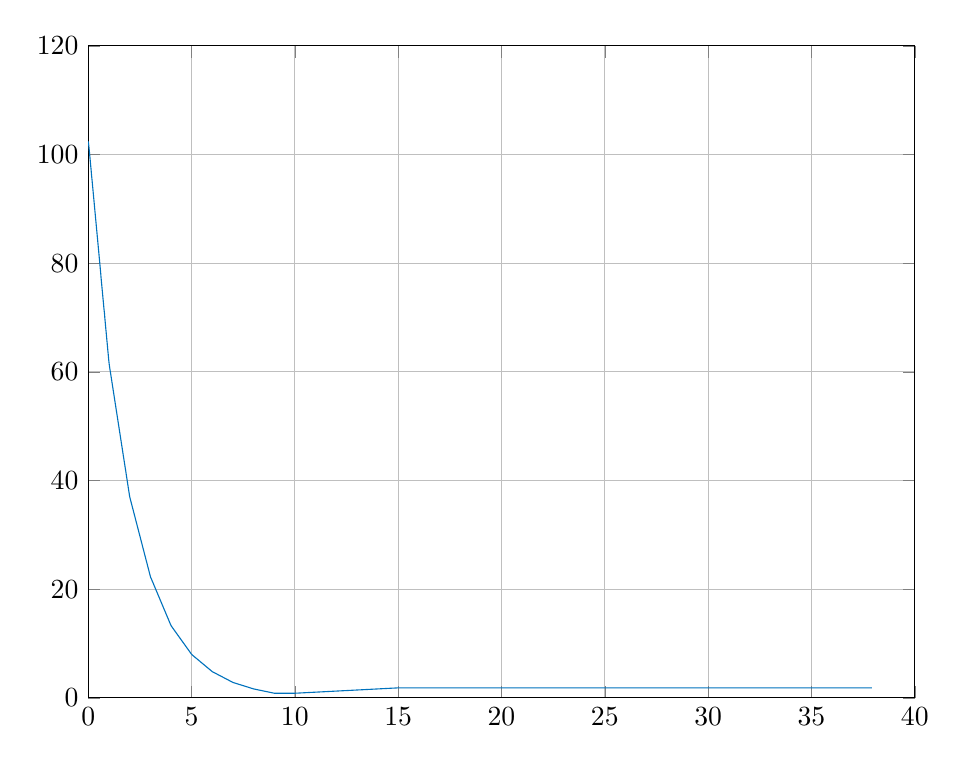
\begin{tikzpicture}

\begin{axis}[%
width=4.133in,
height=3.26in,
at={(0.693in,0.44in)},
scale only axis,
xmin=0,
xmax=40,
xmajorgrids,
ymin=0,
ymax=120,
ymajorgrids,
axis background/.style={fill=white}
]
\addplot [color=mycolor1,solid,forget plot]
  table[row sep=crcr]{%
0	102.4204\\
0.0175286090010004	102.0304\\
0.0327141810000008	101.5084\\
0.0479910410000002	100.9164\\
0.0639312180000003	100.2904\\
0.0799715030010007	99.6564\\
0.0961065930000003	98.9964\\
0.112018136	98.3384\\
0.128039332	97.6884\\
0.143974164999001	97.0404\\
0.159966389	96.2784\\
0.175996244	95.7124\\
0.192504888	95.0504\\
0.207987188	94.4084\\
0.224097574	93.7704\\
0.239858294000001	93.1124\\
0.256018261	92.4644\\
0.271949063	91.8124\\
0.287972994999001	91.1504\\
0.304063760001	90.4924\\
0.319922497	89.8464\\
0.336021966	89.1744\\
0.351947015000001	88.5284\\
0.367970001	87.8844\\
0.384110473	87.2144\\
0.400094109001	86.5664\\
0.416175096000001	85.9184\\
0.432236017000001	85.2664\\
0.448119506999001	84.6144\\
0.463938545	83.9684\\
0.479979641000001	83.3164\\
0.495974428000001	82.6624\\
0.511969809	82.0084\\
0.527904703001	81.3564\\
0.544032905000001	80.7024\\
0.559979558	80.0524\\
0.575969916000999	79.3964\\
0.591956362	78.7404\\
0.607962259	78.0684\\
0.623960694001	77.2544\\
0.639982501	76.6184\\
0.655957017000001	75.9804\\
0.671945996000001	75.3424\\
0.687995782	74.6824\\
0.703974602	74.0304\\
0.720077955	73.3784\\
0.736171671	72.7204\\
0.752021749	72.0644\\
0.768285501	71.4184\\
0.789760393000001	70.7144\\
0.801511386	70.0944\\
0.816647937000001	69.4444\\
0.831948707	68.8004\\
0.847953975998999	68.1484\\
0.864166652999001	67.4984\\
0.880055812000001	66.8424\\
0.896043659999	66.1904\\
0.911885972000001	65.5364\\
0.927999446	64.8924\\
0.94397526	64.2344\\
0.959976189999999	63.5744\\
0.975940821	62.9144\\
0.992110877	62.2624\\
1.010728679	61.6044\\
1.025681988	61.1524\\
1.040599292	60.7804\\
1.055863567999	60.3824\\
1.073925923999	59.9904\\
1.088849986	59.6164\\
1.10402431	59.2364\\
1.119930651002	58.8444\\
1.135954453001	58.4504\\
1.151960149	58.0544\\
1.167957417	57.6664\\
1.183935245	57.2724\\
1.199948839	56.8804\\
1.215973333	56.4884\\
1.231852322	56.0904\\
1.247932156	55.7004\\
1.263968101	55.3044\\
1.280067049	54.9124\\
1.296271842	54.5184\\
1.311953195	54.1224\\
1.328081156001	53.7384\\
1.34409233	53.3344\\
1.359861937999	52.9404\\
1.376075925001	52.5524\\
1.392120594	52.1644\\
1.407849722001	51.7664\\
1.424223779999	51.3744\\
1.440056364	50.9724\\
1.456103514	50.5784\\
1.472240578	50.1924\\
1.488163762	49.8004\\
1.504113848	49.4084\\
1.520035839	49.0144\\
1.53611212	48.6244\\
1.552513494	48.2284\\
1.568058541	47.8324\\
1.58398832	47.4444\\
1.599919621999	47.0464\\
1.616105898	46.6564\\
1.632009909001	46.2644\\
1.648041569	45.8724\\
1.66397886	45.4804\\
1.679951187	45.0744\\
1.695847106	44.6844\\
1.711863424	44.2964\\
1.727908615	43.9084\\
1.743894291	43.5124\\
1.760021833001	43.1184\\
1.776170925001	42.7264\\
1.792047659	42.3264\\
1.810444284	41.9244\\
1.825612141	41.5304\\
1.840813018	41.1424\\
1.855982423999	40.7504\\
1.871950656	40.3644\\
1.88799293	39.9684\\
1.904083343	39.5724\\
1.920004799	39.1824\\
1.935849753	38.7844\\
1.952027522	38.3944\\
1.968020756999	38.0044\\
1.983988911001	37.6124\\
2.000002921	37.1904\\
2.017440971	36.8664\\
2.03252348	36.6524\\
2.047995194	36.4204\\
2.063976379	36.1944\\
2.079989031	35.9624\\
2.09625605	35.7224\\
2.111982437001	35.4824\\
2.128035855	35.2564\\
2.143953996	35.0224\\
2.160036773	34.7944\\
2.176123221	34.5564\\
2.191966392001	34.3244\\
2.208029635999	34.0904\\
2.224031694	33.8544\\
2.240083665001	33.6204\\
2.255973207	33.3844\\
2.271934838999	33.1404\\
2.287894067	32.9124\\
2.303891527001	32.6784\\
2.319961300001	32.4464\\
2.335933588999	32.2164\\
2.351936301	31.9784\\
2.368001882001	31.7444\\
2.383812085002	31.5084\\
2.399965391	31.2764\\
2.416030181	31.0384\\
2.431873823	30.8044\\
2.447959182	30.5684\\
2.463916408001	30.3364\\
2.479944520999	30.1044\\
2.495934807001	29.8664\\
2.512037302	29.6384\\
2.527984836999	29.3984\\
2.543949837	29.1664\\
2.559928947	28.9284\\
2.576031576001	28.6924\\
2.591929896	28.4564\\
2.607945303999	28.2264\\
2.623982417	27.9784\\
2.639972779	27.7504\\
2.6559522	27.5144\\
2.672217134	27.2824\\
2.687930303	27.0504\\
2.703968713	26.8144\\
2.719941154	26.5824\\
2.735880991	26.3404\\
2.751999974001	26.1064\\
2.767999486	25.8764\\
2.783918805	25.6404\\
2.79993866	25.4064\\
2.815938774001	25.1744\\
2.832100669	24.9384\\
2.848187590001	24.7044\\
2.864131541	24.4664\\
2.880025152999	24.2344\\
2.896126576	23.9984\\
2.912119584	23.7644\\
2.928014023	23.5304\\
2.944095686	23.2904\\
2.960077889	23.0564\\
2.975973471	22.8264\\
2.991930989	22.5944\\
3.00926067	22.3524\\
3.02437794	22.1484\\
3.039871704	22.0264\\
3.055842995	21.8884\\
3.073930683	21.7444\\
3.088951682001	21.5964\\
3.10401803	21.4584\\
3.119870446	21.3184\\
3.138104104	21.1664\\
3.153161135	21.0244\\
3.168342408001	20.8864\\
3.183977739999	20.7384\\
3.199890716	20.5944\\
3.215972475	20.4524\\
3.231937855	20.3064\\
3.247915839	20.1624\\
3.263977516	20.0184\\
3.279971656	19.8744\\
3.295957468	19.7224\\
3.312033338	19.5784\\
3.327932217	19.4364\\
3.343931324	19.2904\\
3.360140747	19.1484\\
3.376345088999	19.0044\\
3.392107213	18.8564\\
3.407962733	18.7124\\
3.424224475	18.5704\\
3.440078839	18.4244\\
3.456101298	18.2804\\
3.471961795	18.1404\\
3.487935765	17.9884\\
3.50394353	17.8444\\
3.519981144001	17.7004\\
3.535939277	17.5584\\
3.551925439	17.4164\\
3.567928114	17.2724\\
3.583963247	17.1224\\
3.600069536001	16.9784\\
3.615931858	16.8364\\
3.632106913	16.6864\\
3.648135313	16.5424\\
3.663874567	16.4004\\
3.679872017	16.2544\\
3.696106274	16.1124\\
3.712153686	15.9684\\
3.728016318	15.8244\\
3.743882515	15.6804\\
3.760228751001	15.5304\\
3.776151304	15.3864\\
3.792116759	15.2444\\
3.808104970999	15.0964\\
3.824162821001	14.9484\\
3.839961947	14.8064\\
3.856010196	14.6624\\
3.874266268	14.5124\\
3.88933892	14.3704\\
3.904853928	14.2324\\
3.920289112	14.0804\\
3.936003678	13.9404\\
3.951929829	13.7964\\
3.967933195	13.6524\\
3.983940048999	13.5124\\
4.002202414999	13.3564\\
4.016432713	13.2344\\
4.031971074999	13.1584\\
4.047958609999	13.0764\\
4.063904075	12.9924\\
4.079940962	12.9064\\
4.095935342	12.8224\\
4.112079012	12.7344\\
4.127950538001	12.6524\\
4.144105659	12.5684\\
4.160118235	12.4804\\
4.176081816001	12.3964\\
4.191838606	12.3104\\
4.207830787	12.2284\\
4.223973751001	12.1444\\
4.240109879	12.0584\\
4.256140982	11.9724\\
4.2721012	11.8864\\
4.288175817999	11.8004\\
4.304072948	11.7164\\
4.319958312	11.6304\\
4.335950909	11.5484\\
4.351963666	11.4644\\
4.368135915001	11.3784\\
4.383911399001	11.2884\\
4.400017152	11.2064\\
4.415870653	11.1244\\
4.431816916	11.0364\\
4.44776153	10.9504\\
4.465901256	10.8644\\
4.481048191001	10.7824\\
4.496348363	10.7004\\
4.512001463	10.6084\\
4.527786227999	10.5224\\
4.543780866001	10.4444\\
4.559935912	10.3584\\
4.57593806	10.2724\\
4.592113161	10.1864\\
4.607967714	10.1044\\
4.623907406	10.0204\\
4.640080316001	9.93039999999999\\
4.656132418	9.84439999999999\\
4.67208585	9.76039999999999\\
4.687962534	9.6764\\
4.70394363	9.5924\\
4.719932423	9.5064\\
4.735935072	9.42240000000001\\
4.751951022	9.34039999999999\\
4.767967062	9.2544\\
4.783941993002	9.16839999999999\\
4.799931147	9.08239999999999\\
4.81611384	8.99839999999999\\
4.832093918	8.91240000000001\\
4.84852122	8.8284\\
4.86411608	8.7444\\
4.879992292	8.66040000000001\\
4.895929313	8.57440000000001\\
4.911967328	8.49039999999999\\
4.927999489	8.4024\\
4.943941236001	8.3184\\
4.960101332	8.23439999999999\\
4.976101881	8.15039999999999\\
4.992100767	8.06440000000001\\
5.013350965	7.97639999999998\\
5.025385894001	7.9204\\
5.040760442999	7.87239999999998\\
5.056057898	7.8244\\
5.071908192999	7.77239999999999\\
5.087937902999	7.7204\\
5.103903890001	7.6704\\
5.119905823	7.62039999999999\\
5.135934826	7.57040000000001\\
5.151954219	7.52039999999998\\
5.167932758999	7.4704\\
5.184007857	7.4164\\
5.199937095001	7.36839999999998\\
5.215939725	7.3184\\
5.231930267	7.26839999999999\\
5.248093720001	7.21639999999999\\
5.264164459	7.16240000000001\\
5.279948527999	7.1104\\
5.295936539999	7.06039999999999\\
5.311913862	7.01039999999999\\
5.327945517	6.96040000000001\\
5.344056366001	6.91240000000001\\
5.359936899001	6.8604\\
5.375935824999	6.80839999999998\\
5.391949564	6.76039999999999\\
5.408045484999	6.71040000000001\\
5.424112105	6.66039999999998\\
5.44001592	6.60839999999999\\
5.456114737	6.55639999999998\\
5.472211109	6.5044\\
5.48810844	6.45439999999999\\
5.504085035	6.40239999999999\\
5.519989126	6.3524\\
5.536113281	6.30239999999999\\
5.552126920001	6.25039999999998\\
5.568095708	6.2004\\
5.584173768	6.1484\\
5.600117203	6.0984\\
5.616144138	6.04839999999999\\
5.632115802	6.00039999999998\\
5.648085211	5.9504\\
5.664002907	5.8964\\
5.679918174	5.84439999999999\\
5.695970336	5.7944\\
5.712192272001	5.7444\\
5.728124081001	5.69239999999999\\
5.744109556	5.64239999999999\\
5.759993937	5.5904\\
5.776073091	5.54040000000001\\
5.791971935	5.49039999999999\\
5.807985920001	5.4404\\
5.823936336	5.39039999999999\\
5.839959291	5.3404\\
5.856130122	5.2884\\
5.871992007001	5.23839999999998\\
5.887942508999	5.1844\\
5.904133218999	5.13639999999999\\
5.920023724001	5.08439999999999\\
5.935938184	5.03439999999998\\
5.952108348	4.98439999999999\\
5.968109352	4.9344\\
5.983933756999	4.8784\\
5.999951833	4.8304\\
6.017378119	4.78639999999999\\
6.032499056	4.75839999999999\\
6.048105261	4.72839999999999\\
6.06393357	4.6964\\
6.079930151002	4.6644\\
6.095937962	4.6284\\
6.111920677	4.5984\\
6.128128942	4.5684\\
6.144204871999	4.5384\\
6.159827649	4.5044\\
6.176134244	4.4744\\
6.19218159	4.4404\\
6.208131248999	4.41040000000001\\
6.223997038001	4.3784\\
6.240072770999	4.34639999999999\\
6.256102524	4.31439999999999\\
6.272067288	4.28039999999999\\
6.287924307	4.2504\\
6.303931106	4.2204\\
6.320157612	4.1884\\
6.336412409	4.15839999999999\\
6.352078956001	4.1264\\
6.368004045001	4.0924\\
6.383935272	4.06039999999999\\
6.399927263	4.02839999999999\\
6.416249631	3.9984\\
6.432049601	3.9684\\
6.448142210002	3.93439999999998\\
6.463953049	3.90039999999999\\
6.479897272	3.8704\\
6.496117584	3.83840000000001\\
6.512073468	3.80839999999999\\
6.528131838	3.7764\\
6.544228781	3.74640000000001\\
6.560108828	3.71040000000001\\
6.576437777	3.68039999999999\\
6.592085918	3.6484\\
6.608108117	3.61839999999998\\
6.624084256	3.58840000000001\\
6.640063714	3.55439999999999\\
6.656111174	3.52039999999998\\
6.67208153	3.49039999999999\\
6.687788259	3.45639999999999\\
6.703929447	3.42639999999999\\
6.719934091	3.3984\\
6.735929479	3.36439999999999\\
6.751915069999	3.3304\\
6.767894511	3.3004\\
6.784074558	3.26839999999999\\
6.799997477	3.23839999999998\\
6.816076142999	3.2064\\
6.831891317	3.1724\\
6.848087586	3.14039999999999\\
6.864116805001	3.1104\\
6.879988092	3.0784\\
6.895941534999	3.04839999999999\\
6.912085534999	3.01439999999999\\
6.928161861	2.9804\\
6.944082966	2.95039999999999\\
6.960130772999	2.91839999999999\\
6.976077938	2.88839999999999\\
6.992051931	2.85839999999999\\
7.013066508999	2.8244\\
7.025127625	2.80239999999999\\
7.040665732	2.7824\\
7.056214572999	2.76639999999999\\
7.072085569	2.7484\\
7.08810866	2.7304\\
7.104109675	2.71040000000001\\
7.119775165001	2.69239999999999\\
7.136050227	2.6704\\
7.151964876999	2.65239999999999\\
7.167928763	2.63239999999999\\
7.18398415	2.61439999999999\\
7.200094015	2.59439999999999\\
7.216357040001	2.57639999999999\\
7.2320756	2.55839999999999\\
7.24795692	2.5384\\
7.263938847001	2.52039999999998\\
7.279926221	2.50239999999999\\
7.295889246	2.4804\\
7.311927461	2.4624\\
7.327973584	2.44239999999999\\
7.344056185	2.4224\\
7.359842945	2.40639999999999\\
7.376016773	2.38839999999999\\
7.391933911001	2.36839999999998\\
7.408007102001	2.3484\\
7.423948157	2.3304\\
7.439963229001	2.31039999999999\\
7.455927191001	2.2924\\
7.472110455	2.27239999999999\\
7.488181119	2.25239999999999\\
7.504122343	2.2324\\
7.52009035	2.21639999999999\\
7.535917255001	2.1944\\
7.551912448	2.17639999999999\\
7.567998787	2.1584\\
7.584025034999	2.13839999999999\\
7.600099251	2.12239999999998\\
7.616126667	2.1024\\
7.631940303	2.08240000000001\\
7.647996840001	2.0624\\
7.664099661	2.0424\\
7.68000459	2.02439999999999\\
7.69593747	2.0064\\
7.711930844	1.98839999999998\\
7.727935974001	1.9684\\
7.744172543001	1.94839999999999\\
7.760053802001	1.92839999999998\\
7.776105493002	1.91240000000001\\
7.791991508	1.89239999999999\\
7.808079346	1.87239999999998\\
7.823950001	1.8524\\
7.839826798	1.8344\\
7.856021149	1.8164\\
7.872101065	1.79639999999999\\
7.887964907	1.77839999999999\\
7.903819206	1.75839999999999\\
7.919981061	1.73839999999998\\
7.935846024	1.72240000000001\\
7.951820589	1.70239999999998\\
7.967829414	1.68239999999999\\
7.983884009	1.66240000000001\\
8.002266858	1.64239999999999\\
8.016551753999	1.6264\\
8.032504569	1.61439999999999\\
8.047887354001	1.6044\\
8.063857638	1.5904\\
8.079866456	1.57839999999999\\
8.095848203	1.5664\\
8.111998266	1.55439999999999\\
8.12805133	1.5384\\
8.143944686	1.52839999999999\\
8.159974673001	1.51439999999999\\
8.175944854001	1.50239999999999\\
8.191945764	1.48839999999998\\
8.207943788	1.4764\\
8.223894876	1.4644\\
8.239950059	1.45039999999999\\
8.255977931	1.4384\\
8.271995887	1.42439999999999\\
8.28788622	1.41240000000001\\
8.303949471	1.40039999999999\\
8.319973128	1.38839999999999\\
8.3359204	1.37440000000001\\
8.351946214	1.36239999999999\\
8.368118032	1.3484\\
8.383980278	1.3364\\
8.400151279	1.3244\\
8.416422352	1.3124\\
8.432083893	1.29839999999999\\
8.448113048001	1.2864\\
8.464109864	1.27239999999999\\
8.480090684	1.26039999999999\\
8.496082218	1.2484\\
8.512110335	1.23439999999999\\
8.528156975	1.22239999999999\\
8.543879128	1.20839999999998\\
8.560133623	1.19839999999999\\
8.576008979	1.18439999999998\\
8.591973555999	1.1724\\
8.60804589	1.1584\\
8.624150024	1.1464\\
8.639943705	1.13239999999999\\
8.655787328001	1.1224\\
8.671899676	1.10839999999999\\
8.687933256	1.09639999999999\\
8.703930979001	1.08239999999998\\
8.720113426	1.07039999999999\\
8.736124935999	1.05839999999999\\
8.752033527	1.0444\\
8.76813281	1.03240000000001\\
8.784082845001	1.01839999999999\\
8.799957029	1.00839999999999\\
8.81600476	0.994400000000013\\
8.831939907	0.982399999999998\\
8.847977225	0.968400000000003\\
8.863952687	0.956399999999988\\
8.879979817	0.944400000000002\\
8.895934578	0.930399999999992\\
8.912093637	0.918399999999991\\
8.92810439	0.906399999999991\\
8.944107721	0.89439999999999\\
8.960103855	0.878399999999999\\
8.975951413	0.86839999999998\\
8.991965388	0.854399999999998\\
9.009352886	0.842399999999998\\
9.024450024001	0.840400000000002\\
9.040002202	0.840400000000002\\
9.056010775	0.840400000000002\\
9.072114803999	0.840400000000002\\
9.08786798	0.840400000000002\\
9.103937579	0.840400000000002\\
9.119934149	0.840400000000002\\
9.135939475	0.840400000000002\\
9.15194022	0.840400000000002\\
9.168101062999	0.840400000000002\\
9.184045435	0.840400000000002\\
9.200115678	0.840400000000002\\
9.216090665001	0.840400000000002\\
9.232163468	0.840400000000002\\
9.248114531	0.840400000000002\\
9.264084025	0.840400000000002\\
9.28011347	0.840400000000002\\
9.296107916	0.840400000000002\\
9.312237658001	0.840400000000002\\
9.328130098	0.840400000000002\\
9.34399035	0.840400000000002\\
9.360104005001	0.840400000000002\\
9.376082956	0.840400000000002\\
9.39211384	0.840400000000002\\
9.408069587	0.840400000000002\\
9.424067211	0.840400000000002\\
9.440343024	0.840400000000002\\
9.456068510999	0.840400000000002\\
9.471895301	0.840400000000002\\
9.488082559	0.840400000000002\\
9.504124703	0.840400000000002\\
9.520347727001	0.840400000000002\\
9.536091689999	0.840400000000002\\
9.552100819001	0.840400000000002\\
9.568138147	0.840400000000002\\
9.583960437	0.840400000000002\\
9.599923397	0.840400000000002\\
9.615798262001	0.840400000000002\\
9.631820195	0.840400000000002\\
9.647822662	0.840400000000002\\
9.663832367	0.840400000000002\\
9.679931898	0.840400000000002\\
9.695915725	0.840400000000002\\
9.711889259	0.840400000000002\\
9.727818351	0.840400000000002\\
9.743798975	0.840400000000002\\
9.761959826001	0.840400000000002\\
9.776972461999	0.840400000000002\\
9.792267152	0.840400000000002\\
9.808100613	0.840400000000002\\
9.824028302001	0.840400000000002\\
9.840087789999	0.840400000000002\\
9.8561104	0.840400000000002\\
9.872121418999	0.840400000000002\\
9.888155314	0.840400000000002\\
9.904082367	0.840400000000002\\
9.920240974001	0.840400000000002\\
9.936121051	0.840400000000002\\
9.952097586	0.840400000000002\\
9.96811531	0.840400000000002\\
9.984080149	0.840400000000002\\
9.999965918	0.842399999999998\\
10.017486288	0.842399999999998\\
10.032695398	0.848399999999998\\
10.048114731	0.850399999999993\\
10.064102176	0.852399999999989\\
10.080262186	0.856399999999994\\
10.095831754	0.860399999999998\\
10.111948071	0.862399999999994\\
10.128226406	0.864399999999989\\
10.14400839	0.870400000000004\\
10.160049231	0.872399999999999\\
10.176091435	0.874400000000009\\
10.191956307	0.878399999999999\\
10.207948453	0.880399999999995\\
10.223978614001	0.88239999999999\\
10.239944265	0.888400000000004\\
10.255907573	0.8904\\
10.271970947	0.892399999999995\\
10.287930058	0.898399999999995\\
10.304111478	0.900399999999991\\
10.320114117	0.902399999999986\\
10.336119563	0.9084\\
10.35214322	0.910399999999996\\
10.368096783001	0.912400000000005\\
10.384105867	0.916399999999996\\
10.400055581001	0.920400000000001\\
10.416123341	0.922399999999996\\
10.432107611	0.926399999999987\\
10.448070249	0.930399999999992\\
10.464197381	0.932399999999987\\
10.480115128001	0.934399999999982\\
10.496072865	0.938399999999987\\
10.511988814001	0.942399999999992\\
10.527948626	0.944400000000002\\
10.544043078	0.948399999999992\\
10.559970798	0.950399999999988\\
10.575934201	0.952399999999983\\
10.591921663	0.958400000000012\\
10.607927710002	0.960400000000007\\
10.623817831999	0.962400000000002\\
10.639924365	0.968400000000003\\
10.655895718	0.970399999999998\\
10.67186442	0.972399999999993\\
10.687958552	0.976399999999984\\
10.704102763	0.980400000000003\\
10.719882869	0.982399999999998\\
10.735790912	0.986399999999989\\
10.754054316001	0.990399999999994\\
10.769355776	0.992399999999989\\
10.784545012	0.994399999999985\\
10.799942655	1.0004\\
10.815940989999	1.00239999999999\\
10.831970675001	1.0044\\
10.847952106	1.00839999999999\\
10.86382174	1.01039999999999\\
10.879850498	1.01439999999999\\
10.895937228	1.0184\\
10.911824384	1.0204\\
10.927871223	1.02239999999999\\
10.944060239999	1.0284\\
10.960013098	1.0304\\
10.975906139	1.03240000000001\\
10.991909105	1.0384\\
11.013126152	1.04040000000001\\
11.025047916999	1.0424\\
11.040254703001	1.04639999999999\\
11.056147413	1.0504\\
11.072111420001	1.05239999999999\\
11.088228895	1.0564\\
11.104116193	1.06039999999999\\
11.120145708001	1.0624\\
11.135940316001	1.06440000000001\\
11.152109708	1.0684\\
11.168104069	1.07239999999999\\
11.184110271	1.0744\\
11.200066584	1.07839999999999\\
11.216215166	1.08039999999998\\
11.231936638	1.08239999999998\\
11.247838072999	1.08840000000001\\
11.264074672	1.0904\\
11.280085265	1.0924\\
11.296117407	1.0984\\
11.311959752	1.10039999999999\\
11.328148197999	1.10239999999999\\
11.344102501999	1.10639999999999\\
11.360193207	1.1104\\
11.376082479001	1.11239999999999\\
11.391872441001	1.11639999999998\\
11.407835758	1.1204\\
11.423998223	1.1224\\
11.439917263	1.12440000000001\\
11.455990262	1.13039999999999\\
11.472217716	1.13239999999999\\
11.488112365	1.1344\\
11.503954837	1.1384\\
11.520000935	1.14239999999999\\
11.535952589	1.14239999999999\\
11.551972257001	1.1484\\
11.56800566	1.15039999999999\\
11.583932604	1.15239999999999\\
11.599955023	1.1584\\
11.615964072	1.1604\\
11.631939018	1.16240000000001\\
11.64800441	1.1664\\
11.663944823	1.1704\\
11.67992888	1.1724\\
11.695925085002	1.17639999999999\\
11.711936931	1.18039999999999\\
11.728147817	1.18239999999999\\
11.744108416	1.18639999999999\\
11.759914936	1.19039999999998\\
11.775940477	1.19239999999999\\
11.791903111001	1.1944\\
11.807905194	1.19839999999999\\
11.824081121001	1.20239999999998\\
11.840119762001	1.20440000000001\\
11.856157345	1.20840000000001\\
11.872121618	1.21040000000001\\
11.888143359999	1.2124\\
11.904145644	1.2184\\
11.919892915001	1.2204\\
11.936045899999	1.22239999999999\\
11.951935208001	1.22839999999999\\
11.967951352	1.2304\\
11.983942836	1.2324\\
12.000027667	1.23639999999999\\
12.017479912	1.24039999999999\\
12.032743096	1.24239999999999\\
12.048065784	1.24639999999999\\
12.063855402	1.2504\\
12.079907652999	1.25239999999999\\
12.095873077	1.2544\\
12.112107692001	1.26039999999999\\
12.128135819001	1.26239999999999\\
12.144188597001	1.26439999999999\\
12.159976184	1.2684\\
12.175967222001	1.2704\\
12.192020817	1.27439999999999\\
12.208178923999	1.2784\\
12.224079357	1.2804\\
12.240113312	1.28240000000001\\
12.256273548999	1.2884\\
12.27194383	1.29040000000001\\
12.287932858	1.2924\\
12.304108956	1.29839999999999\\
12.320140621	1.3004\\
12.336150081	1.30239999999999\\
12.352111707	1.3064\\
12.368116982	1.31039999999999\\
12.384118279	1.3124\\
12.399949369	1.3164\\
12.416084840001	1.32039999999999\\
12.432080589	1.32239999999999\\
12.448173587	1.3244\\
12.464110453	1.32839999999999\\
12.479958091	1.33239999999998\\
12.496014593	1.3344\\
12.512055413001	1.33840000000001\\
12.52809867	1.3424\\
12.544089257001	1.3424\\
12.559953588	1.3484\\
12.575947713	1.35039999999999\\
12.591885634	1.35239999999999\\
12.607836673001	1.35839999999999\\
12.623888534001	1.3604\\
12.639939077	1.36239999999999\\
12.656047115	1.36639999999998\\
12.671948951	1.3704\\
12.687984159	1.3724\\
12.703995123	1.3764\\
12.720046763	1.38039999999999\\
12.736008394	1.38239999999999\\
12.752366706999	1.3844\\
12.768060641	1.3884\\
12.784101305	1.39239999999999\\
12.800570271	1.39439999999999\\
12.81633199	1.3984\\
12.832110626	1.40039999999999\\
12.848438763	1.40439999999998\\
12.864039982999	1.4084\\
12.879937524	1.4104\\
12.895959381999	1.41240000000001\\
12.911931126	1.41839999999999\\
12.927927281	1.4204\\
12.943920158001	1.4224\\
12.959893938	1.42639999999999\\
12.975940517001	1.43039999999999\\
12.991923672	1.43239999999999\\
13.010272609	1.43639999999999\\
13.025367431	1.44039999999998\\
13.040510501999	1.44239999999999\\
13.056148234	1.4464\\
13.072172803	1.45039999999999\\
13.088086786999	1.45239999999998\\
13.104179089	1.4564\\
13.120153134	1.45840000000001\\
13.136094564001	1.4624\\
13.152013814	1.4644\\
13.167932875	1.4684\\
13.184222347	1.47239999999999\\
13.199875241	1.47239999999999\\
13.215944775	1.47839999999999\\
13.231853192	1.4804\\
13.247990492	1.4824\\
13.263839724001	1.48839999999998\\
13.279981012001	1.49039999999999\\
13.295924709	1.49239999999999\\
13.311898407	1.49639999999999\\
13.328046205	1.5004\\
13.343891383999	1.50239999999999\\
13.359833099001	1.5064\\
13.376003268	1.51039999999999\\
13.392036146	1.51239999999999\\
13.407888542	1.51439999999999\\
13.42383248	1.5204\\
13.439839475	1.52239999999999\\
13.457931702	1.52439999999999\\
13.472948095	1.5284\\
13.488257173	1.5304\\
13.503823027	1.53440000000001\\
13.522050584	1.5384\\
13.53719658	1.54040000000001\\
13.552538494	1.5424\\
13.567998868	1.54839999999999\\
13.583804119	1.5504\\
13.601910115	1.55239999999999\\
13.616918983	1.55839999999999\\
13.631829595	1.56039999999999\\
13.649985368002	1.5624\\
13.665012856	1.5664\\
13.680428652	1.57039999999999\\
13.69589344	1.57239999999999\\
13.711879787	1.57639999999999\\
13.727847685999	1.58039999999998\\
13.743822405	1.58239999999998\\
13.759998213999	1.5844\\
13.775832821	1.58840000000001\\
13.793940617	1.5924\\
13.809082241	1.59439999999999\\
13.824148361	1.5984\\
13.839842748001	1.60039999999999\\
13.855830987	1.60239999999999\\
13.873901219	1.60839999999999\\
13.888930148	1.6104\\
13.903808384	1.61239999999999\\
13.921912498	1.61839999999998\\
13.936957769	1.6204\\
13.951832513	1.6224\\
13.969888547	1.6284\\
13.984873113	1.63039999999999\\
13.999855701	1.63239999999999\\
14.015854496	1.63639999999999\\
14.033905699	1.6404\\
14.048776798	1.64239999999999\\
14.063806402	1.64439999999999\\
14.081875208	1.65039999999999\\
14.096918632001	1.65239999999999\\
14.112324129	1.65439999999998\\
14.127829152	1.6584\\
14.143852312999	1.6604\\
14.159828986	1.6644\\
14.175891214	1.66839999999999\\
14.191849248	1.6704\\
14.207874261	1.6724\\
14.223846579	1.67839999999998\\
14.239813201	1.68039999999999\\
14.257845945	1.68239999999999\\
14.272723831001	1.68839999999999\\
14.28783551	1.69039999999998\\
14.303814675999	1.69239999999999\\
14.319801096	1.6964\\
14.338138301	1.70039999999999\\
14.353340656	1.70239999999998\\
14.368396336	1.7064\\
14.384002921	1.71040000000001\\
14.399952124	1.7124\\
14.415875197	1.7144\\
14.434150929	1.7204\\
14.449298581	1.72239999999999\\
14.46441684	1.72439999999999\\
14.479792654	1.72839999999999\\
14.496004258	1.7304\\
14.51202553	1.7324\\
14.527979253	1.73839999999998\\
14.543987681	1.74039999999999\\
14.559980603	1.74239999999999\\
14.575942355	1.74839999999999\\
14.591965696	1.7504\\
14.607930805	1.75239999999999\\
14.623944966	1.7564\\
14.640054051	1.76039999999999\\
14.656084744	1.76239999999999\\
14.672349788	1.76639999999999\\
14.688146982	1.7704\\
14.703785914	1.77239999999999\\
14.720082438	1.77439999999999\\
14.736043369	1.7804\\
14.751979516	1.78240000000001\\
14.768240166	1.78440000000001\\
14.784146016	1.7884\\
14.799901389	1.7924\\
14.815870342	1.7924\\
14.831881969	1.79839999999999\\
14.848114843	1.8004\\
14.864130016	1.80239999999999\\
14.880159146	1.80839999999999\\
14.896200963999	1.81039999999999\\
14.912131259	1.8124\\
14.928168256999	1.8184\\
14.944154753999	1.82039999999999\\
14.960260793	1.82239999999999\\
14.976126404001	1.82639999999999\\
14.992190942	1.83039999999998\\
15.013139666	1.83039999999998\\
15.025057657	1.83039999999998\\
15.040338085	1.83039999999998\\
15.056129641	1.83039999999998\\
15.071995736001	1.83039999999998\\
15.088024784999	1.83039999999998\\
15.104200642	1.83039999999998\\
15.120069949	1.83039999999998\\
15.135948818	1.83039999999998\\
15.151956284	1.83039999999998\\
15.168105906	1.83039999999998\\
15.184183225	1.83039999999998\\
15.200161459	1.83039999999998\\
15.216218291	1.83039999999998\\
15.232119404999	1.83039999999998\\
15.248092197	1.83039999999998\\
15.264143677	1.83039999999998\\
15.280102011	1.83039999999998\\
15.295933743	1.83039999999998\\
15.312139798	1.83039999999998\\
15.328098543	1.83039999999998\\
15.344006603	1.83039999999998\\
15.360074851	1.83039999999998\\
15.376219468	1.83039999999998\\
15.392110609	1.83039999999998\\
15.408009673999	1.83039999999998\\
15.424113137	1.83039999999998\\
15.439982705	1.83039999999998\\
15.45863335	1.83039999999998\\
15.47421709	1.83039999999998\\
15.49001475	1.83039999999998\\
15.505273067	1.83039999999998\\
15.520354977	1.83039999999998\\
15.535883455	1.83039999999998\\
15.552149581001	1.83039999999998\\
15.567880439	1.83039999999998\\
15.584028138	1.83039999999998\\
15.599967534	1.83039999999998\\
15.616080689	1.83039999999998\\
15.632082075	1.83039999999998\\
15.648101703	1.83039999999998\\
15.664183626999	1.83039999999998\\
15.680086441001	1.83039999999998\\
15.695946221	1.83039999999998\\
15.71193775	1.83039999999998\\
15.727872919	1.83039999999998\\
15.744006505	1.83039999999998\\
15.760046812	1.83039999999998\\
15.775936263	1.83039999999998\\
15.791821509	1.83039999999998\\
15.807915388	1.83039999999998\\
15.823933606	1.83039999999998\\
15.839910493	1.83039999999998\\
15.858117710002	1.83039999999998\\
15.871954527	1.83039999999998\\
15.887858187	1.83039999999998\\
15.903823322	1.83039999999998\\
15.919939402999	1.83039999999998\\
15.936082566001	1.83039999999998\\
15.952112442	1.83039999999998\\
15.967970377	1.83039999999998\\
15.983945595999	1.83039999999998\\
15.999912654	1.83039999999998\\
16.017529342	1.83039999999998\\
16.032696102	1.83039999999998\\
16.047917914	1.83039999999998\\
16.063881758	1.83039999999998\\
16.079874965	1.83039999999998\\
16.095940523	1.83039999999998\\
16.11189139	1.83039999999998\\
16.127959869	1.83039999999998\\
16.143944612	1.83039999999998\\
16.159903718	1.83039999999998\\
16.175959473	1.83039999999998\\
16.191945258999	1.83039999999998\\
16.207929627	1.83039999999998\\
16.223856084	1.83039999999998\\
16.239977522	1.83039999999998\\
16.255986236	1.83039999999998\\
16.271979904999	1.83039999999998\\
16.287967044	1.83039999999998\\
16.303984933	1.83039999999998\\
16.319974573	1.83039999999998\\
16.335950602	1.83039999999998\\
16.351963654999	1.83039999999998\\
16.367943252	1.83039999999998\\
16.383934265001	1.83039999999998\\
16.399932464	1.83039999999998\\
16.416481627	1.83039999999998\\
16.43211311	1.83039999999998\\
16.447842341	1.83039999999998\\
16.463901589	1.83039999999998\\
16.479856454	1.83039999999998\\
16.496067074	1.83039999999998\\
16.512091047	1.83039999999998\\
16.528113934	1.83039999999998\\
16.544009985	1.83039999999998\\
16.560075422	1.83039999999998\\
16.576102417	1.83039999999998\\
16.592197135001	1.83039999999998\\
16.608271256	1.83039999999998\\
16.623888957	1.83039999999998\\
16.63995888	1.83039999999998\\
16.655929998	1.83039999999998\\
16.672078041999	1.83039999999998\\
16.688101919	1.83039999999998\\
16.704105706	1.83039999999998\\
16.719947456	1.83039999999998\\
16.736224562001	1.83039999999998\\
16.751968821	1.83039999999998\\
16.767946815	1.83039999999998\\
16.784092092	1.83039999999998\\
16.800207637	1.83039999999998\\
16.815885468	1.83039999999998\\
16.832102536	1.83039999999998\\
16.848094651002	1.83039999999998\\
16.864120679	1.83039999999998\\
16.880119991	1.83039999999998\\
16.896114597001	1.83039999999998\\
16.912097151	1.83039999999998\\
16.928103754	1.83039999999998\\
16.943910131	1.83039999999998\\
16.959951356	1.83039999999998\\
16.975928567	1.83039999999998\\
16.991932109	1.83039999999998\\
17.010296029999	1.83039999999998\\
17.025509275	1.83039999999998\\
17.040596184	1.83039999999998\\
17.05616497	1.83039999999998\\
17.071942604001	1.83039999999998\\
17.088092282	1.83039999999998\\
17.104036078001	1.83039999999998\\
17.120077325	1.83039999999998\\
17.136088925	1.83039999999998\\
17.151868859999	1.83039999999998\\
17.167906732	1.83039999999998\\
17.18386933	1.83039999999998\\
17.200147541	1.83039999999998\\
17.216180549	1.83039999999998\\
17.232083593	1.83039999999998\\
17.247773334	1.83039999999998\\
17.263872717	1.83039999999998\\
17.279873586	1.83039999999998\\
17.296084068	1.83039999999998\\
17.312116559	1.83039999999998\\
17.328070589	1.83039999999998\\
17.343875658001	1.83039999999998\\
17.359988965999	1.83039999999998\\
17.376016103	1.83039999999998\\
17.392102481	1.83039999999998\\
17.407993624	1.83039999999998\\
17.42406886	1.83039999999998\\
17.439919725	1.83039999999998\\
17.455862553	1.83039999999998\\
17.471947926	1.83039999999998\\
17.48783825	1.83039999999998\\
17.50379668	1.83039999999998\\
17.522040149	1.83039999999998\\
17.537082145	1.83039999999998\\
17.552161612	1.83039999999998\\
17.567915173	1.83039999999998\\
17.583944026002	1.83039999999998\\
17.599956834	1.83039999999998\\
17.615930793	1.83039999999998\\
17.632110975	1.83039999999998\\
17.648149565	1.83039999999998\\
17.664140448	1.83039999999998\\
17.680102736001	1.83039999999998\\
17.696108102	1.83039999999998\\
17.712030459	1.83039999999998\\
17.728116883999	1.83039999999998\\
17.744350446001	1.83039999999998\\
17.759968123	1.83039999999998\\
17.775946192	1.83039999999998\\
17.791850180999	1.83039999999998\\
17.807906138	1.83039999999998\\
17.823948643	1.83039999999998\\
17.839951407	1.83039999999998\\
17.856111859	1.83039999999998\\
17.872100457	1.83039999999998\\
17.888071906001	1.83039999999998\\
17.904105806	1.83039999999998\\
17.919799694	1.83039999999998\\
17.938030008	1.83039999999998\\
17.953248907	1.83039999999998\\
17.968342068	1.83039999999998\\
17.983908606	1.83039999999998\\
17.999973962	1.83039999999998\\
18.015899532	1.83039999999998\\
18.031916809	1.83039999999998\\
18.047889919	1.83039999999998\\
18.064116866999	1.83039999999998\\
18.079906526002	1.83039999999998\\
18.095941031001	1.83039999999998\\
18.111943865	1.83039999999998\\
18.127893296	1.83039999999998\\
18.143939505	1.83039999999998\\
18.159985873001	1.83039999999998\\
18.176004729	1.83039999999998\\
18.192016048	1.83039999999998\\
18.207966966	1.83039999999998\\
18.223982234001	1.83039999999998\\
18.239949538	1.83039999999998\\
18.255985643	1.83039999999998\\
18.271990397	1.83039999999998\\
18.287998128	1.83039999999998\\
18.30394446	1.83039999999998\\
18.319941236	1.83039999999998\\
18.335966145999	1.83039999999998\\
18.351949171	1.83039999999998\\
18.367991019	1.83039999999998\\
18.383939942	1.83039999999998\\
18.399939479001	1.83039999999998\\
18.415976967	1.83039999999998\\
18.432077803999	1.83039999999998\\
18.448086933	1.83039999999998\\
18.464107212	1.83039999999998\\
18.480080846	1.83039999999998\\
18.495978989	1.83039999999998\\
18.51195145	1.83039999999998\\
18.528110248	1.83039999999998\\
18.544223879	1.83039999999998\\
18.559957824001	1.83039999999998\\
18.575955913	1.83039999999998\\
18.591947608	1.83039999999998\\
18.607949560999	1.83039999999998\\
18.623917953	1.83039999999998\\
18.640009283001	1.83039999999998\\
18.656125324	1.83039999999998\\
18.671968793001	1.83039999999998\\
18.688096631	1.83039999999998\\
18.704079831	1.83039999999998\\
18.72005214	1.83039999999998\\
18.736103933	1.83039999999998\\
18.752049278	1.83039999999998\\
18.767952326	1.83039999999998\\
18.783989874	1.83039999999998\\
18.799898045	1.83039999999998\\
18.816092800001	1.83039999999998\\
18.83216648	1.83039999999998\\
18.848043560999	1.83039999999998\\
18.864081053	1.83039999999998\\
18.880154246999	1.83039999999998\\
18.896000100999	1.83039999999998\\
18.911961122	1.83039999999998\\
18.927999722	1.83039999999998\\
18.943941835	1.83039999999998\\
18.959912621999	1.83039999999998\\
18.97593669	1.83039999999998\\
18.991992725	1.83039999999998\\
19.009771218999	1.83039999999998\\
19.025005593	1.83039999999998\\
19.040206249	1.83039999999998\\
19.055972879	1.83039999999998\\
19.071954515	1.83039999999998\\
19.087941349001	1.83039999999998\\
19.103959934	1.83039999999998\\
19.119938986	1.83039999999998\\
19.135901529	1.83039999999998\\
19.151884519	1.83039999999998\\
19.167925925999	1.83039999999998\\
19.183870333999	1.83039999999998\\
19.200100579	1.83039999999998\\
19.215843759	1.83039999999998\\
19.232109847	1.83039999999998\\
19.248136771	1.83039999999998\\
19.263856832	1.83039999999998\\
19.280108253	1.83039999999998\\
19.296178029001	1.83039999999998\\
19.31198026	1.83039999999998\\
19.327935807	1.83039999999998\\
19.344110732	1.83039999999998\\
19.360100031	1.83039999999998\\
19.376326803	1.83039999999998\\
19.391963383	1.83039999999998\\
19.408030197999	1.83039999999998\\
19.424096191001	1.83039999999998\\
19.440124123001	1.83039999999998\\
19.456286739999	1.83039999999998\\
19.471952004	1.83039999999998\\
19.488108899	1.83039999999998\\
19.503960621	1.83039999999998\\
19.519949113	1.83039999999998\\
19.535931702	1.83039999999998\\
19.551951725999	1.83039999999998\\
19.568016867	1.83039999999998\\
19.583978967	1.83039999999998\\
19.599992473	1.83039999999998\\
19.615947397	1.83039999999998\\
19.631911324999	1.83039999999998\\
19.647869396	1.83039999999998\\
19.663926607999	1.83039999999998\\
19.679929616001	1.83039999999998\\
19.696054722001	1.83039999999998\\
19.711879600999	1.83039999999998\\
19.728022674	1.83039999999998\\
19.744017306	1.83039999999998\\
19.759967544	1.83039999999998\\
19.77604992	1.83039999999998\\
19.79205802	1.83039999999998\\
19.808145935999	1.83039999999998\\
19.823986046	1.83039999999998\\
19.839842619999	1.83039999999998\\
19.855804391	1.83039999999998\\
19.871840807001	1.83039999999998\\
19.887898645	1.83039999999998\\
19.903982821001	1.83039999999998\\
19.919934159	1.83039999999998\\
19.935944301	1.83039999999998\\
19.951919633	1.83039999999998\\
19.967940584	1.83039999999998\\
19.983936027	1.83039999999998\\
19.999936617	1.83039999999998\\
20.017335581	1.83039999999998\\
20.032502922	1.83039999999998\\
20.047973124	1.83039999999998\\
20.063934746	1.83039999999998\\
20.079932389	1.83039999999998\\
20.0959227	1.83039999999998\\
20.111955664	1.83039999999998\\
20.127938949	1.83039999999998\\
20.143902625	1.83039999999998\\
20.159912741	1.83039999999998\\
20.175979321	1.83039999999998\\
20.191976102001	1.83039999999998\\
20.207982074	1.83039999999998\\
20.223940347	1.83039999999998\\
20.239912663001	1.83039999999998\\
20.255917768	1.83039999999998\\
20.271951979001	1.83039999999998\\
20.287931972	1.83039999999998\\
20.303954095	1.83039999999998\\
20.319933217	1.83039999999998\\
20.335963168	1.83039999999998\\
20.35194491	1.83039999999998\\
20.368115470001	1.83039999999998\\
20.384151881	1.83039999999998\\
20.4002472	1.83039999999998\\
20.416253166999	1.83039999999998\\
20.432052987	1.83039999999998\\
20.448099781001	1.83039999999998\\
20.463856852999	1.83039999999998\\
20.48010727	1.83039999999998\\
20.496118379	1.83039999999998\\
20.51220781	1.83039999999998\\
20.527944822	1.83039999999998\\
20.543923783001	1.83039999999998\\
20.559964539	1.83039999999998\\
20.576116849001	1.83039999999998\\
20.592152887	1.83039999999998\\
20.608242739	1.83039999999998\\
20.624031715	1.83039999999998\\
20.640187506	1.83039999999998\\
20.656110961	1.83039999999998\\
20.672092534999	1.83039999999998\\
20.688079416	1.83039999999998\\
20.703999678999	1.83039999999998\\
20.720002423	1.83039999999998\\
20.736132747	1.83039999999998\\
20.752039043	1.83039999999998\\
20.768113661	1.83039999999998\\
20.784041083999	1.83039999999998\\
20.799827843999	1.83039999999998\\
20.81582435	1.83039999999998\\
20.831930892	1.83039999999998\\
20.847925278	1.83039999999998\\
20.864134754	1.83039999999998\\
20.880179878999	1.83039999999998\\
20.896057595999	1.83039999999998\\
20.911911508	1.83039999999998\\
20.927960492	1.83039999999998\\
20.943985501999	1.83039999999998\\
20.959885945	1.83039999999998\\
20.975939139	1.83039999999998\\
20.991941999	1.83039999999998\\
21.009779437	1.83039999999998\\
21.024882588001	1.83039999999998\\
21.040045449	1.83039999999998\\
21.055946824001	1.83039999999998\\
21.071977118	1.83039999999998\\
21.08791806	1.83039999999998\\
21.103921159999	1.83039999999998\\
21.119894233	1.83039999999998\\
21.135928078001	1.83039999999998\\
21.151933248	1.83039999999998\\
21.168037969	1.83039999999998\\
21.183936191001	1.83039999999998\\
21.199956576001	1.83039999999998\\
21.21600325	1.83039999999998\\
21.232109565	1.83039999999998\\
21.248029582	1.83039999999998\\
21.264104225	1.83039999999998\\
21.280177494	1.83039999999998\\
21.296243061	1.83039999999998\\
21.312106565	1.83039999999998\\
21.327891859	1.83039999999998\\
21.344217879	1.83039999999998\\
21.360107342	1.83039999999998\\
21.376108959	1.83039999999998\\
21.392171284	1.83039999999998\\
21.407972470999	1.83039999999998\\
21.424108067001	1.83039999999998\\
21.440053905	1.83039999999998\\
21.456081787	1.83039999999998\\
21.471908734	1.83039999999998\\
21.487872933	1.83039999999998\\
21.503806279	1.83039999999998\\
21.519997151	1.83039999999998\\
21.53602173	1.83039999999998\\
21.552145329	1.83039999999998\\
21.567807281001	1.83039999999998\\
21.583790090001	1.83039999999998\\
21.60199432	1.83039999999998\\
21.617019604	1.83039999999998\\
21.632168267999	1.83039999999998\\
21.648120006	1.83039999999998\\
21.663954314	1.83039999999998\\
21.679898396	1.83039999999998\\
21.695945867	1.83039999999998\\
21.712085437	1.83039999999998\\
21.728038158001	1.83039999999998\\
21.744080964	1.83039999999998\\
21.760195025	1.83039999999998\\
21.776113258001	1.83039999999998\\
21.792066852	1.83039999999998\\
21.808074557	1.83039999999998\\
21.824042312999	1.83039999999998\\
21.839914386	1.83039999999998\\
21.856096723	1.83039999999998\\
21.872407987	1.83039999999998\\
21.888112099001	1.83039999999998\\
21.903899451	1.83039999999998\\
21.919880265001	1.83039999999998\\
21.936124916	1.83039999999998\\
21.952073842	1.83039999999998\\
21.967986696001	1.83039999999998\\
21.984148217	1.83039999999998\\
22.000118989	1.83039999999998\\
22.017667460002	1.83039999999998\\
22.032873849001	1.83039999999998\\
22.047979282	1.83039999999998\\
22.064129807	1.83039999999998\\
22.079995345999	1.83039999999998\\
22.095936431	1.83039999999998\\
22.111935011	1.83039999999998\\
22.128108748	1.83039999999998\\
22.144052925	1.83039999999998\\
22.160082229	1.83039999999998\\
22.176119217	1.83039999999998\\
22.192095717	1.83039999999998\\
22.207963355	1.83039999999998\\
22.223953847	1.83039999999998\\
22.239907937001	1.83039999999998\\
22.256038449	1.83039999999998\\
22.272045245	1.83039999999998\\
22.287937549	1.83039999999998\\
22.303917011	1.83039999999998\\
22.319946796	1.83039999999998\\
22.335948393	1.83039999999998\\
22.352103699	1.83039999999998\\
22.368279526	1.83039999999998\\
22.384079651	1.83039999999998\\
22.400080251	1.83039999999998\\
22.415971276	1.83039999999998\\
22.432422739	1.83039999999998\\
22.448073645999	1.83039999999998\\
22.464112583	1.83039999999998\\
22.480105435	1.83039999999998\\
22.496115501	1.83039999999998\\
22.512127156	1.83039999999998\\
22.527992277999	1.83039999999998\\
22.543901047	1.83039999999998\\
22.559880489999	1.83039999999998\\
22.575877373	1.83039999999998\\
22.591889157	1.83039999999998\\
22.607989379	1.83039999999998\\
22.624225973	1.83039999999998\\
22.639927048999	1.83039999999998\\
22.655963423	1.83039999999998\\
22.671942384	1.83039999999998\\
22.68800648	1.83039999999998\\
22.70401181	1.83039999999998\\
22.719825713	1.83039999999998\\
22.736094333999	1.83039999999998\\
22.75201397	1.83039999999998\\
22.768004201001	1.83039999999998\\
22.783926223	1.83039999999998\\
22.802168378001	1.83039999999998\\
22.817357735	1.83039999999998\\
22.832176942	1.83039999999998\\
22.847923558	1.83039999999998\\
22.863804336	1.83039999999998\\
22.879757817	1.83039999999998\\
22.895821710002	1.83039999999998\\
22.911989203	1.83039999999998\\
22.928039395	1.83039999999998\\
22.944099424	1.83039999999998\\
22.960026713	1.83039999999998\\
22.975844172	1.83039999999998\\
22.991885821	1.83039999999998\\
23.009436458	1.83039999999998\\
23.024682809	1.83039999999998\\
23.040034166999	1.83039999999998\\
23.05602273	1.83039999999998\\
23.072096460002	1.83039999999998\\
23.088091983	1.83039999999998\\
23.104105347001	1.83039999999998\\
23.120040694001	1.83039999999998\\
23.136075661	1.83039999999998\\
23.152122877	1.83039999999998\\
23.168140255	1.83039999999998\\
23.184100643	1.83039999999998\\
23.200145589	1.83039999999998\\
23.215960583	1.83039999999998\\
23.231926794	1.83039999999998\\
23.24793851	1.83039999999998\\
23.263963981	1.83039999999998\\
23.280083856	1.83039999999998\\
23.296100872	1.83039999999998\\
23.312153691001	1.83039999999998\\
23.328157548	1.83039999999998\\
23.34401782	1.83039999999998\\
23.360068077	1.83039999999998\\
23.376175333	1.83039999999998\\
23.392109457	1.83039999999998\\
23.408024678999	1.83039999999998\\
23.424309217	1.83039999999998\\
23.440059625	1.83039999999998\\
23.455847446	1.83039999999998\\
23.472088141	1.83039999999998\\
23.488079284	1.83039999999998\\
23.504120671	1.83039999999998\\
23.520026481	1.83039999999998\\
23.535957998999	1.83039999999998\\
23.552072381999	1.83039999999998\\
23.568110537	1.83039999999998\\
23.583953425001	1.83039999999998\\
23.599949574	1.83039999999998\\
23.615931482	1.83039999999998\\
23.631933339	1.83039999999998\\
23.647937026	1.83039999999998\\
23.663983269001	1.83039999999998\\
23.679952772999	1.83039999999998\\
23.695921531001	1.83039999999998\\
23.711888710002	1.83039999999998\\
23.727822734	1.83039999999998\\
23.743820661999	1.83039999999998\\
23.759825955	1.83039999999998\\
23.775943052	1.83039999999998\\
23.791941847	1.83039999999998\\
23.807932094	1.83039999999998\\
23.823943002	1.83039999999998\\
23.839928377	1.83039999999998\\
23.855937571	1.83039999999998\\
23.871920636	1.83039999999998\\
23.887933589	1.83039999999998\\
23.903945098	1.83039999999998\\
23.920188102001	1.83039999999998\\
23.936095872	1.83039999999998\\
23.952009835	1.83039999999998\\
23.967876176	1.83039999999998\\
23.983930227	1.83039999999998\\
23.999937822	1.83039999999998\\
24.017380871	1.83039999999998\\
24.032552773	1.83039999999998\\
24.047959066001	1.83039999999998\\
24.06395526	1.83039999999998\\
24.079945442	1.83039999999998\\
24.095911538	1.83039999999998\\
24.112064789	1.83039999999998\\
24.128099421	1.83039999999998\\
24.143953485	1.83039999999998\\
24.160175765	1.83039999999998\\
24.176077566001	1.83039999999998\\
24.191949790001	1.83039999999998\\
24.207935286	1.83039999999998\\
24.223936797	1.83039999999998\\
24.239957778	1.83039999999998\\
24.256010566001	1.83039999999998\\
24.271917654	1.83039999999998\\
24.288078803	1.83039999999998\\
24.304105938	1.83039999999998\\
24.320013902	1.83039999999998\\
24.336142623	1.83039999999998\\
24.352105562	1.83039999999998\\
24.368073363	1.83039999999998\\
24.384130115	1.83039999999998\\
24.40021503	1.83039999999998\\
24.415966761	1.83039999999998\\
24.431995899	1.83039999999998\\
24.447891001	1.83039999999998\\
24.463933906999	1.83039999999998\\
24.479882218	1.83039999999998\\
24.495937717	1.83039999999998\\
24.511969377	1.83039999999998\\
24.527924529	1.83039999999998\\
24.543931679	1.83039999999998\\
24.560011072	1.83039999999998\\
24.575929831	1.83039999999998\\
24.591924062	1.83039999999998\\
24.608025535	1.83039999999998\\
24.623925812	1.83039999999998\\
24.639937978	1.83039999999998\\
24.656250229001	1.83039999999998\\
24.671978452	1.83039999999998\\
24.687939447	1.83039999999998\\
24.704083772	1.83039999999998\\
24.719924189	1.83039999999998\\
24.735958084	1.83039999999998\\
24.751959847001	1.83039999999998\\
24.767966766	1.83039999999998\\
24.784146517	1.83039999999998\\
24.800117439	1.83039999999998\\
24.816031838	1.83039999999998\\
24.831922148	1.83039999999998\\
24.847945128	1.83039999999998\\
24.863913159	1.83039999999998\\
24.880215624	1.83039999999998\\
24.896159389	1.83039999999998\\
24.912103115	1.83039999999998\\
24.928148612	1.83039999999998\\
24.944273639	1.83039999999998\\
24.959953511	1.83039999999998\\
24.976074218	1.83039999999998\\
24.991964302	1.83039999999998\\
25.009645892001	1.83039999999998\\
25.024828347	1.83039999999998\\
25.04010196	1.83039999999998\\
25.055947002	1.83039999999998\\
25.072009451001	1.83039999999998\\
25.087962424	1.83039999999998\\
25.103933151	1.83039999999998\\
25.119928223	1.83039999999998\\
25.135936215001	1.83039999999998\\
25.151954123	1.83039999999998\\
25.16796738	1.83039999999998\\
25.183944889	1.83039999999998\\
25.199915446	1.83039999999998\\
25.215955355	1.83039999999998\\
25.231933093	1.83039999999998\\
25.248081217	1.83039999999998\\
25.264171614999	1.83039999999998\\
25.280082491	1.83039999999998\\
25.296073715001	1.83039999999998\\
25.31186524	1.83039999999998\\
25.327974898	1.83039999999998\\
25.344000258	1.83039999999998\\
25.359913057	1.83039999999998\\
25.375957668999	1.83039999999998\\
25.39193672	1.83039999999998\\
25.408013818	1.83039999999998\\
25.423951931	1.83039999999998\\
25.440128946	1.83039999999998\\
25.456071379	1.83039999999998\\
25.472101285	1.83039999999998\\
25.488070995	1.83039999999998\\
25.50411392	1.83039999999998\\
25.520116013	1.83039999999998\\
25.535959567	1.83039999999998\\
25.551919996	1.83039999999998\\
25.567963914	1.83039999999998\\
25.583939662	1.83039999999998\\
25.600127706999	1.83039999999998\\
25.615960987	1.83039999999998\\
25.631957442	1.83039999999998\\
25.647929047	1.83039999999998\\
25.663933545	1.83039999999998\\
25.679933885	1.83039999999998\\
25.695962718	1.83039999999998\\
25.712207897	1.83039999999998\\
25.728150456	1.83039999999998\\
25.744114663001	1.83039999999998\\
25.760119432	1.83039999999998\\
25.776165755	1.83039999999998\\
25.791940558	1.83039999999998\\
25.807927898	1.83039999999998\\
25.824096348	1.83039999999998\\
25.840052692	1.83039999999998\\
25.85600152	1.83039999999998\\
25.872077405	1.83039999999998\\
25.887902357	1.83039999999998\\
25.903881773	1.83039999999998\\
25.920087033001	1.83039999999998\\
25.936074598	1.83039999999998\\
25.952061828	1.83039999999998\\
25.967988644001	1.83039999999998\\
25.984204096	1.83039999999998\\
25.999939096	1.83039999999998\\
26.017576435	1.83039999999998\\
26.032735797	1.83039999999998\\
26.047980794	1.83039999999998\\
26.063982697	1.83039999999998\\
26.079976476	1.83039999999998\\
26.095997377	1.83039999999998\\
26.111968986001	1.83039999999998\\
26.127979212	1.83039999999998\\
26.143953953	1.83039999999998\\
26.159973426	1.83039999999998\\
26.175938144001	1.83039999999998\\
26.191965159	1.83039999999998\\
26.207967362	1.83039999999998\\
26.223961603	1.83039999999998\\
26.239971368002	1.83039999999998\\
26.255977641	1.83039999999998\\
26.271941713	1.83039999999998\\
26.287931859	1.83039999999998\\
26.304016399	1.83039999999998\\
26.320109147	1.83039999999998\\
26.336216539	1.83039999999998\\
26.352005213001	1.83039999999998\\
26.367946844	1.83039999999998\\
26.384071446	1.83039999999998\\
26.400112422	1.83039999999998\\
26.415963357	1.83039999999998\\
26.431951494	1.83039999999998\\
26.447956934	1.83039999999998\\
26.463953766	1.83039999999998\\
26.479941350999	1.83039999999998\\
26.49593725	1.83039999999998\\
26.512055466	1.83039999999998\\
26.528258941001	1.83039999999998\\
26.544029038	1.83039999999998\\
26.56009682	1.83039999999998\\
26.576109102	1.83039999999998\\
26.592588702	1.83039999999998\\
26.607979549	1.83039999999998\\
26.623924333	1.83039999999998\\
26.639940182	1.83039999999998\\
26.655954923999	1.83039999999998\\
26.671990002	1.83039999999998\\
26.688081267001	1.83039999999998\\
26.704080197999	1.83039999999998\\
26.719948959	1.83039999999998\\
26.735951122	1.83039999999998\\
26.752048303	1.83039999999998\\
26.768364331	1.83039999999998\\
26.784623031001	1.83039999999998\\
26.800396014	1.83039999999998\\
26.815803027999	1.83039999999998\\
26.834250033001	1.83039999999998\\
26.849678045001	1.83039999999998\\
26.864880501	1.83039999999998\\
26.880352603	1.83039999999998\\
26.896104008	1.83039999999998\\
26.911974267	1.83039999999998\\
26.927960329	1.83039999999998\\
26.944049845	1.83039999999998\\
26.960099862	1.83039999999998\\
26.976129308	1.83039999999998\\
26.99212923	1.83039999999998\\
27.010021297	1.83039999999998\\
27.025502479	1.83039999999998\\
27.041140793	1.83039999999998\\
27.056740489001	1.83039999999998\\
27.07206183	1.83039999999998\\
27.087988512	1.83039999999998\\
27.104101722	1.83039999999998\\
27.120095566001	1.83039999999998\\
27.136102811	1.83039999999998\\
27.152250128	1.83039999999998\\
27.168085838999	1.83039999999998\\
27.183873489001	1.83039999999998\\
27.200104769	1.83039999999998\\
27.216012399001	1.83039999999998\\
27.232085527	1.83039999999998\\
27.248116391	1.83039999999998\\
27.264102106	1.83039999999998\\
27.280117394001	1.83039999999998\\
27.295944581	1.83039999999998\\
27.311941122	1.83039999999998\\
27.330196998	1.83039999999998\\
27.345483414	1.83039999999998\\
27.360600296	1.83039999999998\\
27.375843434	1.83039999999998\\
27.391875969	1.83039999999998\\
27.407922127	1.83039999999998\\
27.423994011	1.83039999999998\\
27.4399791	1.83039999999998\\
27.455939784	1.83039999999998\\
27.472131637001	1.83039999999998\\
27.488115159	1.83039999999998\\
27.504024421	1.83039999999998\\
27.520105749	1.83039999999998\\
27.536121654	1.83039999999998\\
27.552099056	1.83039999999998\\
27.567849265	1.83039999999998\\
27.584063071	1.83039999999998\\
27.600148883999	1.83039999999998\\
27.616168816001	1.83039999999998\\
27.632266848	1.83039999999998\\
27.648134807	1.83039999999998\\
27.664067381999	1.83039999999998\\
27.680421576	1.83039999999998\\
27.696127892001	1.83039999999998\\
27.711833059	1.83039999999998\\
27.727861015999	1.83039999999998\\
27.746088906	1.83039999999998\\
27.761113671	1.83039999999998\\
27.776263008	1.83039999999998\\
27.792219208999	1.83039999999998\\
27.809013283001	1.83039999999998\\
27.8250579	1.83039999999998\\
27.840154974001	1.83039999999998\\
27.855805468	1.83039999999998\\
27.872045609999	1.83039999999998\\
27.888042821	1.83039999999998\\
27.903883291	1.83039999999998\\
27.920041969	1.83039999999998\\
27.936089064	1.83039999999998\\
27.953072135	1.83039999999998\\
27.968054033001	1.83039999999998\\
27.983786949	1.83039999999998\\
28.001891444001	1.83039999999998\\
28.016120534	1.83039999999998\\
28.031833328	1.83039999999998\\
28.047810061	1.83039999999998\\
28.064037654999	1.83039999999998\\
28.080041357999	1.83039999999998\\
28.096987524001	1.83039999999998\\
28.111871197	1.83039999999998\\
28.127792364	1.83039999999998\\
28.143836368	1.83039999999998\\
28.159875677	1.83039999999998\\
28.175847072	1.83039999999998\\
28.191817587	1.83039999999998\\
28.209915932	1.83039999999998\\
28.224832141	1.83039999999998\\
28.239836255	1.83039999999998\\
28.25787873	1.83039999999998\\
28.272782996999	1.83039999999998\\
28.287804745	1.83039999999998\\
28.30591068	1.83039999999998\\
28.320731984	1.83039999999998\\
28.335895896	1.83039999999998\\
28.351948291999	1.83039999999998\\
28.367850327	1.83039999999998\\
28.383828112	1.83039999999998\\
28.401935869	1.83039999999998\\
28.416950728	1.83039999999998\\
28.431947589	1.83039999999998\\
28.448163132001	1.83039999999998\\
28.463811197	1.83039999999998\\
28.481908388	1.83039999999998\\
28.49682793	1.83039999999998\\
28.511848711	1.83039999999998\\
28.529912354001	1.83039999999998\\
28.545108375	1.83039999999998\\
28.560116108	1.83039999999998\\
28.575819973	1.83039999999998\\
28.593846796	1.83039999999998\\
28.608752771	1.83039999999998\\
28.623856035	1.83039999999998\\
28.639820072999	1.83039999999998\\
28.657933868	1.83039999999998\\
28.672867539999	1.83039999999998\\
28.687919192	1.83039999999998\\
28.705962744	1.83039999999998\\
28.720862844	1.83039999999998\\
28.735840711	1.83039999999998\\
28.754018671	1.83039999999998\\
28.768922725	1.83039999999998\\
28.783832595	1.83039999999998\\
28.79980611	1.83039999999998\\
28.817861911	1.83039999999998\\
28.832832833001	1.83039999999998\\
28.847925613	1.83039999999998\\
28.863924373	1.83039999999998\\
28.880039242	1.83039999999998\\
28.896080348	1.83039999999998\\
28.911916695	1.83039999999998\\
28.927902722	1.83039999999998\\
28.943915976	1.83039999999998\\
28.959841664	1.83039999999998\\
28.977958081	1.83039999999998\\
28.992843300999	1.83039999999998\\
29.009876756	1.83039999999998\\
29.024990196001	1.83039999999998\\
29.041591307	1.83039999999998\\
29.056911350999	1.83039999999998\\
29.072182756	1.83039999999998\\
29.087960367	1.83039999999998\\
29.103945231	1.83039999999998\\
29.120032231	1.83039999999998\\
29.135981465	1.83039999999998\\
29.151993716	1.83039999999998\\
29.16783465	1.83039999999998\\
29.184013954	1.83039999999998\\
29.199948724001	1.83039999999998\\
29.215932301	1.83039999999998\\
29.231942146	1.83039999999998\\
29.247940851	1.83039999999998\\
29.263990658001	1.83039999999998\\
29.279982623	1.83039999999998\\
29.295947567	1.83039999999998\\
29.311938099001	1.83039999999998\\
29.327934339	1.83039999999998\\
29.343936768	1.83039999999998\\
29.359948367	1.83039999999998\\
29.375934840001	1.83039999999998\\
29.391865251	1.83039999999998\\
29.408061729	1.83039999999998\\
29.423983611	1.83039999999998\\
29.439942967	1.83039999999998\\
29.45594271	1.83039999999998\\
29.471935562	1.83039999999998\\
29.487964281	1.83039999999998\\
29.503940284	1.83039999999998\\
29.519932619999	1.83039999999998\\
29.536112536999	1.83039999999998\\
29.552106345999	1.83039999999998\\
29.56810432	1.83039999999998\\
29.583965378	1.83039999999998\\
29.599940935999	1.83039999999998\\
29.61600302	1.83039999999998\\
29.631943138	1.83039999999998\\
29.64816514	1.83039999999998\\
29.664106254	1.83039999999998\\
29.680003941001	1.83039999999998\\
29.695928263	1.83039999999998\\
29.711950056	1.83039999999998\\
29.728101036	1.83039999999998\\
29.744124217	1.83039999999998\\
29.760007526002	1.83039999999998\\
29.776101772999	1.83039999999998\\
29.792077276002	1.83039999999998\\
29.808115350999	1.83039999999998\\
29.823881896	1.83039999999998\\
29.839773017	1.83039999999998\\
29.856012909	1.83039999999998\\
29.871784468999	1.83039999999998\\
29.887932193	1.83039999999998\\
29.903926177	1.83039999999998\\
29.920139344	1.83039999999998\\
29.936099437	1.83039999999998\\
29.952001317999	1.83039999999998\\
29.967911911	1.83039999999998\\
29.984038975	1.83039999999998\\
29.999965753001	1.83039999999998\\
30.017471203	1.83039999999998\\
30.032624291999	1.83039999999998\\
30.047984876	1.83039999999998\\
30.063838902999	1.83039999999998\\
30.079923692	1.83039999999998\\
30.095842666	1.83039999999998\\
30.113855965001	1.83039999999998\\
30.128694831001	1.83039999999998\\
30.143870388	1.83039999999998\\
30.159881641	1.83039999999998\\
30.176931743002	1.83039999999998\\
30.192261054	1.83039999999998\\
30.208012654	1.83039999999998\\
30.223935298999	1.83039999999998\\
30.239857643	1.83039999999998\\
30.255975419	1.83039999999998\\
30.271971513	1.83039999999998\\
30.287967031	1.83039999999998\\
30.303973013	1.83039999999998\\
30.319982192	1.83039999999998\\
30.335927798001	1.83039999999998\\
30.351987265999	1.83039999999998\\
30.367910636	1.83039999999998\\
30.383960918	1.83039999999998\\
30.399936621	1.83039999999998\\
30.416002815	1.83039999999998\\
30.431976543	1.83039999999998\\
30.447942284	1.83039999999998\\
30.464073720001	1.83039999999998\\
30.48021073	1.83039999999998\\
30.496218595001	1.83039999999998\\
30.512020617	1.83039999999998\\
30.528091509	1.83039999999998\\
30.544108917	1.83039999999998\\
30.560123704	1.83039999999998\\
30.576143081001	1.83039999999998\\
30.592118374	1.83039999999998\\
30.608281026002	1.83039999999998\\
30.62411798	1.83039999999998\\
30.639903502	1.83039999999998\\
30.655869979	1.83039999999998\\
30.672105797	1.83039999999998\\
30.687889514	1.83039999999998\\
30.704001407	1.83039999999998\\
30.720093259	1.83039999999998\\
30.736115508	1.83039999999998\\
30.752029597001	1.83039999999998\\
30.767945349001	1.83039999999998\\
30.783942015	1.83039999999998\\
30.799940294	1.83039999999998\\
30.81593249	1.83039999999998\\
30.831943854	1.83039999999998\\
30.847890873	1.83039999999998\\
30.864079303	1.83039999999998\\
30.880147932	1.83039999999998\\
30.896106246	1.83039999999998\\
30.912109045001	1.83039999999998\\
30.928126343	1.83039999999998\\
30.944102357	1.83039999999998\\
30.960006478	1.83039999999998\\
30.976120220001	1.83039999999998\\
30.991943893	1.83039999999998\\
31.012611907	1.83039999999998\\
31.024456202	1.83039999999998\\
31.040132295	1.83039999999998\\
31.055999648	1.83039999999998\\
31.072251618	1.83039999999998\\
31.088097011	1.83039999999998\\
31.103964288001	1.83039999999998\\
31.120136572	1.83039999999998\\
31.136108196	1.83039999999998\\
31.151950126	1.83039999999998\\
31.167948321	1.83039999999998\\
31.183951696001	1.83039999999998\\
31.199939312	1.83039999999998\\
31.215951678	1.83039999999998\\
31.231951892	1.83039999999998\\
31.247931399001	1.83039999999998\\
31.263940618002	1.83039999999998\\
31.279952744	1.83039999999998\\
31.295930943	1.83039999999998\\
31.311942107	1.83039999999998\\
31.327938908001	1.83039999999998\\
31.344155943	1.83039999999998\\
31.360103578	1.83039999999998\\
31.376116977	1.83039999999998\\
31.392053797	1.83039999999998\\
31.408031881	1.83039999999998\\
31.423943324	1.83039999999998\\
31.439935539	1.83039999999998\\
31.455961115	1.83039999999998\\
31.471934378001	1.83039999999998\\
31.487943743	1.83039999999998\\
31.503931704	1.83039999999998\\
31.519934233	1.83039999999998\\
31.535900184	1.83039999999998\\
31.551788790001	1.83039999999998\\
31.56782222	1.83039999999998\\
31.583839482	1.83039999999998\\
31.599812056	1.83039999999998\\
31.615820065	1.83039999999998\\
31.631928361	1.83039999999998\\
31.647933998001	1.83039999999998\\
31.664123086999	1.83039999999998\\
31.679950729001	1.83039999999998\\
31.695939628001	1.83039999999998\\
31.711955076001	1.83039999999998\\
31.727941869	1.83039999999998\\
31.743895974001	1.83039999999998\\
31.759996901002	1.83039999999998\\
31.775932719	1.83039999999998\\
31.791891769	1.83039999999998\\
31.807947299	1.83039999999998\\
31.824098093999	1.83039999999998\\
31.840180744999	1.83039999999998\\
31.856077985	1.83039999999998\\
31.871964551	1.83039999999998\\
31.887944003	1.83039999999998\\
31.903929138	1.83039999999998\\
31.919965529	1.83039999999998\\
31.935917116999	1.83039999999998\\
31.951941772	1.83039999999998\\
31.968062003	1.83039999999998\\
31.984277434	1.83039999999998\\
32.000096357	1.83039999999998\\
32.018226118002	1.83039999999998\\
32.033627561	1.83039999999998\\
32.049271781	1.83039999999998\\
32.06471117	1.83039999999998\\
32.080137036	1.83039999999998\\
32.096198364	1.83039999999998\\
32.112441734001	1.83039999999998\\
32.127958317001	1.83039999999998\\
32.143943637	1.83039999999998\\
32.160102821001	1.83039999999998\\
32.176013943	1.83039999999998\\
32.19207301	1.83039999999998\\
32.207966818	1.83039999999998\\
32.223951085002	1.83039999999998\\
32.239945727	1.83039999999998\\
32.255915852001	1.83039999999998\\
32.271912142999	1.83039999999998\\
32.287939723	1.83039999999998\\
32.303892134	1.83039999999998\\
32.319950218999	1.83039999999998\\
32.335930568	1.83039999999998\\
32.35194096	1.83039999999998\\
32.367901027999	1.83039999999998\\
32.383907606	1.83039999999998\\
32.399923771	1.83039999999998\\
32.416241429	1.83039999999998\\
32.432146933	1.83039999999998\\
32.448117841	1.83039999999998\\
32.464100756	1.83039999999998\\
32.48011448	1.83039999999998\\
32.496116102	1.83039999999998\\
32.512149633	1.83039999999998\\
32.527994515	1.83039999999998\\
32.544085839	1.83039999999998\\
32.559949889	1.83039999999998\\
32.575957054	1.83039999999998\\
32.591930907	1.83039999999998\\
32.607939645999	1.83039999999998\\
32.623927236001	1.83039999999998\\
32.639932131	1.83039999999998\\
32.656110443	1.83039999999998\\
32.671942010001	1.83039999999998\\
32.688147975	1.83039999999998\\
32.70407367	1.83039999999998\\
32.720115814001	1.83039999999998\\
32.736084772	1.83039999999998\\
32.752173888	1.83039999999998\\
32.768146333	1.83039999999998\\
32.784097121001	1.83039999999998\\
32.799820619	1.83039999999998\\
32.816139267	1.83039999999998\\
32.832273164	1.83039999999998\\
32.84808657	1.83039999999998\\
32.864116265	1.83039999999998\\
32.880091107	1.83039999999998\\
32.89593858	1.83039999999998\\
32.911927758	1.83039999999998\\
32.92793159	1.83039999999998\\
32.944111051	1.83039999999998\\
32.959962698	1.83039999999998\\
32.975960882001	1.83039999999998\\
32.99210396	1.83039999999998\\
33.009925983	1.83039999999998\\
33.025268867	1.83039999999998\\
33.04080789	1.83039999999998\\
33.056335428	1.83039999999998\\
33.072164604	1.83039999999998\\
33.088105889	1.83039999999998\\
33.104096417	1.83039999999998\\
33.119964015001	1.83039999999998\\
33.135937508	1.83039999999998\\
33.152072803	1.83039999999998\\
33.168320884	1.83039999999998\\
33.184093748	1.83039999999998\\
33.200142336	1.83039999999998\\
33.21610511	1.83039999999998\\
33.231960185	1.83039999999998\\
33.247941656	1.83039999999998\\
33.263972875	1.83039999999998\\
33.279941177	1.83039999999998\\
33.295951468999	1.83039999999998\\
33.311944481	1.83039999999998\\
33.327912698	1.83039999999998\\
33.343958379	1.83039999999998\\
33.359941084	1.83039999999998\\
33.375932016	1.83039999999998\\
33.391936069001	1.83039999999998\\
33.407961986	1.83039999999998\\
33.424032715	1.83039999999998\\
33.439899927001	1.83039999999998\\
33.455906716	1.83039999999998\\
33.471844586	1.83039999999998\\
33.487828581	1.83039999999998\\
33.50381005	1.83039999999998\\
33.519901461	1.83039999999998\\
33.535949553	1.83039999999998\\
33.551961764	1.83039999999998\\
33.567928649	1.83039999999998\\
33.583994895999	1.83039999999998\\
33.600071513	1.83039999999998\\
33.615834226	1.83039999999998\\
33.631815607	1.83039999999998\\
33.647825128999	1.83039999999998\\
33.664102239	1.83039999999998\\
33.6801079	1.83039999999998\\
33.696106685001	1.83039999999998\\
33.71207417	1.83039999999998\\
33.727960531	1.83039999999998\\
33.743937968	1.83039999999998\\
33.759980297	1.83039999999998\\
33.775931275	1.83039999999998\\
33.79193894	1.83039999999998\\
33.807955972	1.83039999999998\\
33.823940861001	1.83039999999998\\
33.839875004	1.83039999999998\\
33.855879364	1.83039999999998\\
33.871943237	1.83039999999998\\
33.887951339	1.83039999999998\\
33.903934539	1.83039999999998\\
33.920019169	1.83039999999998\\
33.936149283001	1.83039999999998\\
33.952064624	1.83039999999998\\
33.967958337	1.83039999999998\\
33.984099961	1.83039999999998\\
34.000152844	1.83039999999998\\
34.016146001999	1.83039999999998\\
34.032134625	1.83039999999998\\
34.048183539	1.83039999999998\\
34.064219409	1.83039999999998\\
34.08020316	1.83039999999998\\
34.096115369999	1.83039999999998\\
34.112123100999	1.83039999999998\\
34.128077185	1.83039999999998\\
34.143904858	1.83039999999998\\
34.159938954	1.83039999999998\\
34.175884849001	1.83039999999998\\
34.191894819999	1.83039999999998\\
34.208087765999	1.83039999999998\\
34.223967196001	1.83039999999998\\
34.239949685	1.83039999999998\\
34.256076897	1.83039999999998\\
34.272088281	1.83039999999998\\
34.287870343	1.83039999999998\\
34.304070517001	1.83039999999998\\
34.320086126	1.83039999999998\\
34.335855871	1.83039999999998\\
34.35199427	1.83039999999998\\
34.368065339	1.83039999999998\\
34.383926055	1.83039999999998\\
34.39999669	1.83039999999998\\
34.417907877	1.83039999999998\\
34.433029685	1.83039999999998\\
34.448075551	1.83039999999998\\
34.46389136	1.83039999999998\\
34.479913244	1.83039999999998\\
34.495952345001	1.83039999999998\\
34.511987373	1.83039999999998\\
34.527993761	1.83039999999998\\
34.543984689	1.83039999999998\\
34.559999927001	1.83039999999998\\
34.575850052001	1.83039999999998\\
34.591935432	1.83039999999998\\
34.607952414	1.83039999999998\\
34.62394905	1.83039999999998\\
34.639914975999	1.83039999999998\\
34.655949257001	1.83039999999998\\
34.671939317999	1.83039999999998\\
34.687973819	1.83039999999998\\
34.703928801	1.83039999999998\\
34.719881282	1.83039999999998\\
34.735909519	1.83039999999998\\
34.751978027999	1.83039999999998\\
34.767931711	1.83039999999998\\
34.783941777	1.83039999999998\\
34.799942061	1.83039999999998\\
34.815903685	1.83039999999998\\
34.832071962	1.83039999999998\\
34.848231482	1.83039999999998\\
34.864029092	1.83039999999998\\
34.879948432001	1.83039999999998\\
34.895940713999	1.83039999999998\\
34.911941965001	1.83039999999998\\
34.927964103	1.83039999999998\\
34.943846731	1.83039999999998\\
34.959932854001	1.83039999999998\\
34.975956842	1.83039999999998\\
34.992090378	1.83039999999998\\
35.009647621	1.83039999999998\\
35.024907016	1.83039999999998\\
35.040326883999	1.83039999999998\\
35.05616221	1.83039999999998\\
35.072250934	1.83039999999998\\
35.088138638	1.83039999999998\\
35.103874451001	1.83039999999998\\
35.120090220001	1.83039999999998\\
35.136173467	1.83039999999998\\
35.152112587	1.83039999999998\\
35.168122463	1.83039999999998\\
35.184065737	1.83039999999998\\
35.200137404	1.83039999999998\\
35.216282135	1.83039999999998\\
35.232014136	1.83039999999998\\
35.247992977001	1.83039999999998\\
35.264057456	1.83039999999998\\
35.280051935	1.83039999999998\\
35.296124519	1.83039999999998\\
35.312031963	1.83039999999998\\
35.328109839	1.83039999999998\\
35.344028086999	1.83039999999998\\
35.360192402	1.83039999999998\\
35.376016091	1.83039999999998\\
35.392018921	1.83039999999998\\
35.408128849001	1.83039999999998\\
35.424200428999	1.83039999999998\\
35.440127076	1.83039999999998\\
35.456044716	1.83039999999998\\
35.472092911001	1.83039999999998\\
35.488271158001	1.83039999999998\\
35.504125987	1.83039999999998\\
35.52011242	1.83039999999998\\
35.536324861	1.83039999999998\\
35.552281465	1.83039999999998\\
35.568110201	1.83039999999998\\
35.583969983	1.83039999999998\\
35.599978258	1.83039999999998\\
35.616029783001	1.83039999999998\\
35.632015694	1.83039999999998\\
35.648010706	1.83039999999998\\
35.663971842	1.83039999999998\\
35.679962102	1.83039999999998\\
35.695925890999	1.83039999999998\\
35.711976846	1.83039999999998\\
35.727951989001	1.83039999999998\\
35.744027444999	1.83039999999998\\
35.759967151002	1.83039999999998\\
35.776035655	1.83039999999998\\
35.792024949001	1.83039999999998\\
35.808115137001	1.83039999999998\\
35.824087673	1.83039999999998\\
35.840074923	1.83039999999998\\
35.855942040001	1.83039999999998\\
35.871949305	1.83039999999998\\
35.887916289	1.83039999999998\\
35.904052701	1.83039999999998\\
35.920008364001	1.83039999999998\\
35.935958785	1.83039999999998\\
35.952006510999	1.83039999999998\\
35.967825775	1.83039999999998\\
35.986023816001	1.83039999999998\\
36.001234525	1.83039999999998\\
36.016026781001	1.83039999999998\\
36.03186031	1.83039999999998\\
36.047975763	1.83039999999998\\
36.063845549	1.83039999999998\\
36.07992786	1.83039999999998\\
36.095997607001	1.83039999999998\\
36.11197117	1.83039999999998\\
36.127956706	1.83039999999998\\
36.143944892	1.83039999999998\\
36.159989617	1.83039999999998\\
36.175950923	1.83039999999998\\
36.191932174	1.83039999999998\\
36.208014449	1.83039999999998\\
36.223917613	1.83039999999998\\
36.239949198	1.83039999999998\\
36.256039095	1.83039999999998\\
36.271982805	1.83039999999998\\
36.288029615	1.83039999999998\\
36.304048186	1.83039999999998\\
36.31992943	1.83039999999998\\
36.335930234999	1.83039999999998\\
36.351889426	1.83039999999998\\
36.36799807	1.83039999999998\\
36.383937572	1.83039999999998\\
36.399981154001	1.83039999999998\\
36.415990203001	1.83039999999998\\
36.43210445	1.83039999999998\\
36.448127115	1.83039999999998\\
36.464138072999	1.83039999999998\\
36.479939441001	1.83039999999998\\
36.496015552	1.83039999999998\\
36.511945843	1.83039999999998\\
36.528010362	1.83039999999998\\
36.544105306	1.83039999999998\\
36.560085599001	1.83039999999998\\
36.57595386	1.83039999999998\\
36.591981686	1.83039999999998\\
36.608020668001	1.83039999999998\\
36.624012822999	1.83039999999998\\
36.640044082	1.83039999999998\\
36.656036529	1.83039999999998\\
36.672092850001	1.83039999999998\\
36.688065085002	1.83039999999998\\
36.704203833	1.83039999999998\\
36.71994493	1.83039999999998\\
36.735980133	1.83039999999998\\
36.751951847001	1.83039999999998\\
36.768117725999	1.83039999999998\\
36.783876372	1.83039999999998\\
36.802304289	1.83039999999998\\
36.817689705	1.83039999999998\\
36.833211304	1.83039999999998\\
36.848470438	1.83039999999998\\
36.864145840001	1.83039999999998\\
36.880329395	1.83039999999998\\
36.896134681	1.83039999999998\\
36.912423552	1.83039999999998\\
36.928166557001	1.83039999999998\\
36.944013905	1.83039999999998\\
36.960115865	1.83039999999998\\
36.976006919	1.83039999999998\\
36.992156086	1.83039999999998\\
37.010120607	1.83039999999998\\
37.02533762	1.83039999999998\\
37.040498152	1.83039999999998\\
37.056496322	1.83039999999998\\
37.071811442999	1.83039999999998\\
37.08992599	1.83039999999998\\
37.104895731	1.83039999999998\\
37.11991248	1.83039999999998\\
37.135861857	1.83039999999998\\
37.151866013	1.83039999999998\\
37.167918267	1.83039999999998\\
37.186227191001	1.83039999999998\\
37.201288827	1.83039999999998\\
37.216677399	1.83039999999998\\
37.231912525	1.83039999999998\\
37.250033736001	1.83039999999998\\
37.264971586999	1.83039999999998\\
37.280661776002	1.83039999999998\\
37.296189842	1.83039999999998\\
37.312102448	1.83039999999998\\
37.328001066001	1.83039999999998\\
37.343997300999	1.83039999999998\\
37.359859918	1.83039999999998\\
37.376014251	1.83039999999998\\
37.392001782	1.83039999999998\\
37.408039615	1.83039999999998\\
37.423999137001	1.83039999999998\\
37.440067170001	1.83039999999998\\
37.456035381	1.83039999999998\\
37.472047537	1.83039999999998\\
37.487971107	1.83039999999998\\
37.504139672	1.83039999999998\\
37.520097315	1.83039999999998\\
37.536293012	1.83039999999998\\
37.551944756	1.83039999999998\\
37.567958675	1.83039999999998\\
37.583965695	1.83039999999998\\
37.59996189	1.83039999999998\\
37.615923626	1.83039999999998\\
37.631941189	1.83039999999998\\
37.647984927	1.83039999999998\\
37.663953945	1.83039999999998\\
37.679934144	1.83039999999998\\
37.695988588	1.83039999999998\\
37.711938751	1.83039999999998\\
37.727858906001	1.83039999999998\\
37.743815699	1.83039999999998\\
37.761866929	1.83039999999998\\
37.776724973	1.83039999999998\\
37.791802553	1.83039999999998\\
37.809865183	1.83039999999998\\
37.824977214	1.83039999999998\\
37.840059492	1.83039999999998\\
37.855952043001	1.83039999999998\\
37.871895848	1.83039999999998\\
37.903999357	1.83039999999998\\
37.906336396	1.83039999999998\\
37.921276116001	1.83039999999998\\
};
\end{axis}
\end{tikzpicture}%}
      \caption{The error in displacement of the robot over time for
        $(K_{\Psi}^R, K_{\omega}^T) \equiv (0.2 K_{\Psi, max}^R, 0.5 K_{\omega, max}^T)$}
      \label{fig:19_7_distance}
    \end{figure}
  \end{minipage}
  \hfill
  \begin{minipage}{0.45\linewidth}
    \begin{figure}[H]
      \scalebox{0.6}{% This file was created by matlab2tikz.
%
%The latest updates can be retrieved from
%  http://www.mathworks.com/matlabcentral/fileexchange/22022-matlab2tikz-matlab2tikz
%where you can also make suggestions and rate matlab2tikz.
%
\definecolor{mycolor1}{rgb}{0.00000,0.44700,0.74100}%
%
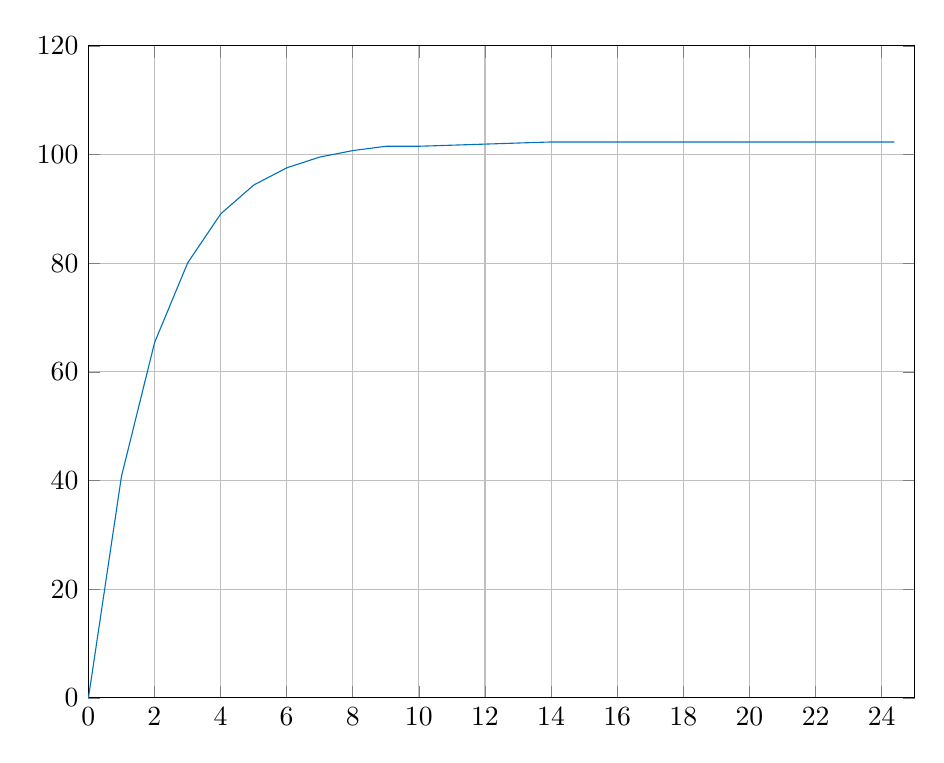
\begin{tikzpicture}

\begin{axis}[%
width=4.133in,
height=3.26in,
at={(0.693in,0.44in)},
scale only axis,
xmin=0,
xmax=25,
xmajorgrids,
ymin=0,
ymax=120,
ymajorgrids,
axis background/.style={fill=white}
]
\addplot [color=mycolor1,solid,forget plot]
  table[row sep=crcr]{%
0	0\\
0.017680273	0.42\\
0.0326910660000006	1.05\\
0.0478512429999998	1.662\\
0.0638764890000001	2.308\\
0.0799588490000004	2.936\\
0.0958651979999999	3.574\\
0.111923665	4.228\\
0.127986862000001	4.882\\
0.144054695	5.534\\
0.159914538999001	6.194\\
0.17601809	6.846\\
0.191946917	7.522\\
0.208079209999001	8.166\\
0.223989928	8.81\\
0.239952898001	9.454\\
0.255942068	10.116\\
0.271942981000001	10.762\\
0.288054942	11.446\\
0.303993131	12.09\\
0.319898738999	12.744\\
0.338376994001	13.416\\
0.354037594000001	14.066\\
0.369093324	14.698\\
0.384204203999001	15.342\\
0.399996272	15.992\\
0.416472500000001	16.648\\
0.431974013999999	17.298\\
0.447922317000001	17.948\\
0.463946346	18.604\\
0.482375421999999	19.286\\
0.497833884000001	19.928\\
0.512944313	20.578\\
0.528342609	21.226\\
0.544029618999	21.868\\
0.55995921	22.53\\
0.576000115000001	23.174\\
0.591977398000999	23.828\\
0.607982704000001	24.48\\
0.624034299001	25.146\\
0.639961316000001	25.792\\
0.655957358	26.45\\
0.67193844	27.096\\
0.688035293000001	27.752\\
0.703973472	28.4\\
0.719969571998999	29.056\\
0.735977464000001	29.704\\
0.752104601000001	30.364\\
0.767968577	31.012\\
0.783949898000001	31.664\\
0.799954111999	32.322\\
0.818500755	33.002\\
0.834119084999	33.65\\
0.849363261000001	34.3\\
0.864831111	34.946\\
0.880055500999001	35.594\\
0.896061910000001	36.268\\
0.911966587999	36.916\\
0.927954776	37.558\\
0.944057603000001	38.204\\
0.960030365000999	38.854\\
0.975909328000001	39.504\\
0.991950462	40.156\\
1.010365616	40.826\\
1.025310158	41.232\\
1.04021214	41.596\\
1.055832138	41.97\\
1.073996943	42.406\\
1.089052950999	42.784\\
1.104370401	43.168\\
1.119958508	43.548\\
1.136001529	43.942\\
1.152015896	44.334\\
1.168022066	44.726\\
1.183979170999	45.118\\
1.200197013	45.51\\
1.216443756	45.908\\
1.231977618999	46.314\\
1.247982273999	46.698\\
1.263959365999	47.104\\
1.280113092999	47.49\\
1.295911162	47.878\\
1.31196283	48.264\\
1.327985997	48.656\\
1.343998571999	49.05\\
1.360053891001	49.442\\
1.376103250999	49.842\\
1.391971526	50.234\\
1.408042054	50.628\\
1.423817408999	51.018\\
1.439809614	51.41\\
1.455967813	51.804\\
1.471980966999	52.198\\
1.488028499	52.592\\
1.503919798	52.982\\
1.519933752	53.372\\
1.535969131	53.786\\
1.552048325	54.16\\
1.567808023	54.554\\
1.586103383	54.96\\
1.601386443	55.36\\
1.616776504	55.744\\
1.632014834	56.146\\
1.648051942	56.532\\
1.664009846	56.94\\
1.679989383	57.33\\
1.695928054	57.716\\
1.711971441	58.108\\
1.728026449	58.492\\
1.744028953999	58.878\\
1.759907247	59.276\\
1.77599245	59.668\\
1.791998698	60.06\\
1.807958127	60.454\\
1.824424295	60.86\\
1.840004503	61.248\\
1.855970019	61.638\\
1.871964281	62.024\\
1.88805972	62.434\\
1.903980575	62.82\\
1.920022889	63.208\\
1.936062658999	63.612\\
1.952027728	64.002\\
1.967967882	64.39\\
1.983977077	64.778\\
1.999971243	65.18\\
2.017336051	65.504\\
2.032277945	65.74\\
2.047807195999	65.972\\
2.065928836	66.208\\
2.080897507	66.434\\
2.096205201	66.674\\
2.111901924001	66.914\\
2.127848016	67.148\\
2.143809912	67.376\\
2.159995884	67.606\\
2.17596372	67.838\\
2.191901353	68.068\\
2.207950236999	68.318\\
2.223912698998	68.546\\
2.240004383	68.776\\
2.256039261001	69.012\\
2.271987563	69.244\\
2.288045899	69.482\\
2.303955608999	69.72\\
2.319981065	69.95\\
2.336020554	70.182\\
2.352036599	70.428\\
2.367874281	70.66\\
2.384005412	70.888\\
2.399965354999	71.13\\
2.418337944	71.37\\
2.433619645	71.602\\
2.449024776999	71.836\\
2.464310233	72.074\\
2.480042389999	72.306\\
2.495855733	72.534\\
2.511935045	72.798\\
2.52801317	73.008\\
2.543960761	73.238\\
2.560007551999	73.474\\
2.577218852	73.712\\
2.592363038999	73.94\\
2.608537794	74.176\\
2.623881354999	74.416\\
2.639813344	74.646\\
2.655850764999	74.88\\
2.671970861	75.108\\
2.688023389	75.344\\
2.703962786	75.586\\
2.719941531999	75.82\\
2.736039162001	76.05\\
2.752034645	76.294\\
2.767942657	76.524\\
2.783951590999	76.752\\
2.799994156	76.998\\
2.818564342	77.234\\
2.833879976	77.468\\
2.849187466	77.71\\
2.864410158999	77.942\\
2.879962665	78.17\\
2.895990482	78.4\\
2.911947939	78.634\\
2.928026912	78.864\\
2.94399345	79.1\\
2.959999292999	79.332\\
2.975969143	79.568\\
2.99202088	79.802\\
3.010108302	80.044\\
3.025081368	80.19\\
3.040024314	80.328\\
3.055884978	80.466\\
3.071866104	80.612\\
3.087985985	80.756\\
3.10395791	80.9\\
3.119972738	81.042\\
3.135995243	81.194\\
3.151954971999	81.338\\
3.167938511999	81.478\\
3.183949997999	81.632\\
3.199971265	81.776\\
3.218263677	81.92\\
3.23336733	82.064\\
3.248597781999	82.206\\
3.263968915	82.35\\
3.279945408	82.49\\
3.29597205	82.636\\
3.311953953	82.784\\
3.328072323	82.932\\
3.343877074	83.074\\
3.360006654	83.216\\
3.376050434	83.36\\
3.391988420999	83.502\\
3.407798753	83.648\\
3.426145757	83.796\\
3.44128471	83.94\\
3.456533712999	84.09\\
3.471957927999	84.23\\
3.488045224	84.374\\
3.50391346	84.512\\
3.519915404	84.66\\
3.535963832	84.802\\
3.552024943	84.948\\
3.568132493	85.092\\
3.584030009	85.244\\
3.599975811	85.388\\
3.618325011	85.536\\
3.633464476	85.676\\
3.648499299	85.82\\
3.663966084999	85.964\\
3.679974157	86.106\\
3.695942165	86.25\\
3.712072573	86.4\\
3.728029519	86.542\\
3.744047623999	86.684\\
3.760059585	86.828\\
3.775967145	86.972\\
3.791942774	87.12\\
3.807987033	87.264\\
3.824035646999	87.404\\
3.839955299001	87.572\\
3.855974437	87.696\\
3.871966052	87.844\\
3.888030948	87.988\\
3.903961064	88.13\\
3.920075611999	88.274\\
3.935961848	88.422\\
3.952074383	88.566\\
3.967997061001	88.71\\
3.983976349	88.862\\
4.00000613	89.004\\
4.015872438	89.116\\
4.031832225	89.198\\
4.049913605	89.286\\
4.064804169	89.374\\
4.07987763	89.452\\
4.09584957	89.538\\
4.114056036	89.63\\
4.129272264999	89.712\\
4.144571130999	89.796\\
4.160011762999	89.882\\
4.175994698	89.964\\
4.191933879001	90.048\\
4.207940907	90.136\\
4.224038089	90.218\\
4.240056825001	90.302\\
4.255865903999	90.386\\
4.271971074	90.476\\
4.288024008	90.56\\
4.304003535001	90.646\\
4.319970054	90.726\\
4.335985147	90.814\\
4.35202982	90.9\\
4.367997512999	90.982\\
4.383987785	91.066\\
4.399978648	91.152\\
4.418318467	91.242\\
4.433488231	91.326\\
4.448518077	91.408\\
4.463987939999	91.49\\
4.479970495	91.578\\
4.495999996	91.66\\
4.511970603	91.746\\
4.528038135	91.83\\
4.544318309	91.918\\
4.559989568	92.002\\
4.575995912	92.086\\
4.591987616999	92.172\\
4.607959491999	92.258\\
4.624002057999	92.34\\
4.639989243	92.442\\
4.655840926	92.514\\
4.672095316	92.598\\
4.688059544	92.684\\
4.703974322	92.766\\
4.719973021	92.852\\
4.736070792	92.938\\
4.751991917	93.022\\
4.767898045	93.106\\
4.78395887	93.19\\
4.799973637999	93.278\\
4.818517439	93.366\\
4.833979399	93.448\\
4.849021412999	93.532\\
4.864259646	93.622\\
4.879993102	93.704\\
4.895872277001	93.788\\
4.911925215999	93.872\\
4.928029561	93.956\\
4.944009736	94.042\\
4.959924648	94.132\\
4.976017842999	94.216\\
4.991972156	94.298\\
5.009711056	94.38\\
5.024677059999	94.436\\
5.039888167	94.484\\
5.055836128	94.532\\
5.073984147	94.586\\
5.089105106	94.634\\
5.104246502	94.682\\
5.119942608	94.732\\
5.135985439	94.782\\
5.152059811	94.836\\
5.168003112	94.888\\
5.183949684999	94.94\\
5.199980669	94.99\\
5.218391725	95.042\\
5.233672379001	95.09\\
5.248932587	95.142\\
5.26420111	95.194\\
5.280057373	95.242\\
5.296098861	95.292\\
5.311996974	95.342\\
5.328238641	95.392\\
5.343935801	95.442\\
5.359932971	95.494\\
5.376004527001	95.546\\
5.391930764	95.598\\
5.407952462999	95.65\\
5.424028168	95.7\\
5.439934475	95.752\\
5.455980132	95.802\\
5.472032675	95.852\\
5.489120174	95.904\\
5.504493998	95.952\\
5.519986061999	96.002\\
5.535995686999	96.054\\
5.552017451	96.104\\
5.567910007	96.152\\
5.583986398	96.206\\
5.599969359	96.256\\
5.616024116999	96.308\\
5.631948084	96.36\\
5.64797575	96.41\\
5.663991946	96.464\\
5.680180051	96.514\\
5.695920792	96.562\\
5.712052385	96.612\\
5.727979985	96.662\\
5.744005250999	96.712\\
5.760018601	96.764\\
5.776021130999	96.814\\
5.792059877	96.864\\
5.807958893	96.914\\
5.823871589	96.968\\
5.83994855	97.018\\
5.855890490999	97.07\\
5.871954158	97.122\\
5.888019719999	97.172\\
5.90396935	97.224\\
5.919949099	97.272\\
5.935963740999	97.324\\
5.951923957	97.374\\
5.967991507	97.424\\
5.983969887999	97.472\\
5.999963360999	97.524\\
6.017773040998	97.568\\
6.032762898	97.598\\
6.047836646	97.628\\
6.065917793	97.668\\
6.080884396999	97.698\\
6.095976695	97.728\\
6.111942401999	97.76\\
6.127898505999	97.79\\
6.143983854	97.82\\
6.159943896999	97.852\\
6.175984071999	97.882\\
6.191960864	97.916\\
6.207946335	97.948\\
6.22404187	97.978\\
6.240049567	98.01\\
6.255975648001	98.042\\
6.271952519999	98.072\\
6.288057527001	98.106\\
6.303945808	98.138\\
6.319890820999	98.168\\
6.335964067	98.2\\
6.352061405	98.232\\
6.368051208	98.266\\
6.383996943999	98.298\\
6.399962766	98.328\\
6.418367762	98.358\\
6.433704043	98.39\\
6.448817063	98.422\\
6.463977054	98.456\\
6.479922316	98.488\\
6.496090253	98.518\\
6.511901181999	98.548\\
6.527948724	98.58\\
6.543927302999	98.614\\
6.560014538	98.646\\
6.575998590999	98.68\\
6.591990330999	98.71\\
6.607993587999	98.74\\
6.624138575	98.77\\
6.639796391	98.804\\
6.655810885	98.838\\
6.671958775	98.868\\
6.687832245999	98.898\\
6.703879021	98.93\\
6.719814221	98.96\\
6.735799123999	98.996\\
6.752032636	99.028\\
6.767863095	99.06\\
6.783961572	99.088\\
6.799961563	99.12\\
6.818635384	99.152\\
6.833845248	99.184\\
6.848982192	99.22\\
6.864138651	99.25\\
6.879969912	99.28\\
6.896009222	99.308\\
6.911965873999	99.342\\
6.927976089001	99.374\\
6.943888625999	99.408\\
6.959959057999	99.44\\
6.975996271	99.472\\
6.991965700999	99.504\\
7.010190373999	99.53\\
7.02516578	99.552\\
7.040083040998	99.572\\
7.05587776	99.592\\
7.074031006999	99.61\\
7.089241464	99.628\\
7.104492828	99.642\\
7.120043349	99.662\\
7.136012433	99.682\\
7.152147071999	99.702\\
7.167816743	99.722\\
7.18385141	99.742\\
7.200009592999	99.762\\
7.216419971	99.778\\
7.231954049	99.798\\
7.247955446999	99.816\\
7.263953702	99.838\\
7.279964825999	99.852\\
7.296009366999	99.872\\
7.311980358999	99.892\\
7.32812326	99.912\\
7.343945589	99.932\\
7.359801431999	99.952\\
7.377894255	99.972\\
7.393848101	99.99\\
7.409007991	100.008\\
7.424261941	100.026\\
7.439904435001	100.044\\
7.455958901999	100.064\\
7.471902821	100.082\\
7.487981717	100.102\\
7.504003670999	100.122\\
7.519833569	100.142\\
7.536008334	100.16\\
7.552069913	100.178\\
7.567971815	100.198\\
7.583958428	100.216\\
7.599926762	100.234\\
7.615856231	100.252\\
7.631944563	100.272\\
7.647822740999	100.292\\
7.663805721	100.312\\
7.679834907	100.332\\
7.69837175	100.352\\
7.713655911	100.37\\
7.728810811	100.39\\
7.744057228	100.408\\
7.759947962999	100.426\\
7.77596421	100.442\\
7.791957849	100.462\\
7.807935082	100.482\\
7.824118280999	100.502\\
7.839977812	100.522\\
7.855950714	100.542\\
7.871981067	100.56\\
7.887868691	100.58\\
7.903940070001	100.596\\
7.919992939999	100.616\\
7.936022527001	100.634\\
7.952053936999	100.654\\
7.967946632	100.672\\
7.983973629	100.692\\
7.999946742	100.712\\
8.017470543	100.728\\
8.032472939	100.742\\
8.047825929999	100.752\\
8.063806795	100.766\\
8.081990717	100.782\\
8.097125396	100.792\\
8.112242545	100.802\\
8.127912986999	100.816\\
8.144102491	100.83\\
8.160020823998	100.842\\
8.175969738	100.854\\
8.192019203999	100.866\\
8.207980415	100.882\\
8.223918835	100.892\\
8.239960939	100.904\\
8.25594192	100.918\\
8.271940892	100.932\\
8.288065453	100.942\\
8.303945736	100.956\\
8.319970536	100.968\\
8.335964682	100.982\\
8.352131769	100.992\\
8.367977529	101.006\\
8.383958729999	101.018\\
8.399990266	101.032\\
8.41835884	101.044\\
8.4335136	101.058\\
8.448628733999	101.072\\
8.463982363	101.082\\
8.480014791	101.096\\
8.495933557	101.108\\
8.511915684999	101.122\\
8.527966446999	101.132\\
8.543992853001	101.146\\
8.560012632	101.16\\
8.576036505	101.172\\
8.591934873999	101.182\\
8.608015996	101.196\\
8.623838475	101.212\\
8.640008523	101.222\\
8.655988566	101.234\\
8.672005599	101.248\\
8.688013045	101.262\\
8.703956264999	101.272\\
8.719973197	101.286\\
8.735986828	101.298\\
8.752038929999	101.312\\
8.76798237	101.322\\
8.783900344	101.336\\
8.799977241999	101.348\\
8.818381818	101.362\\
8.833595232	101.374\\
8.848743259	101.388\\
8.863911002999	101.402\\
8.882369231	101.412\\
8.89768071	101.424\\
8.912734946999	101.438\\
8.928283072	101.452\\
8.94461625	101.462\\
8.959942724	101.476\\
8.975911101	101.49\\
8.991974629	101.502\\
9.009951733	101.51\\
9.024932307	101.512\\
9.039935646	101.512\\
9.055851585	101.512\\
9.071854443	101.512\\
9.088392399999	101.512\\
9.104004668	101.512\\
9.119977181	101.512\\
9.135982849	101.512\\
9.152012214	101.512\\
9.168005002	101.512\\
9.184049021	101.512\\
9.199966979	101.512\\
9.216506855	101.512\\
9.231962924999	101.512\\
9.247925582	101.512\\
9.263996793	101.512\\
9.2799716	101.512\\
9.296033905	101.512\\
9.311952627999	101.512\\
9.328001064	101.512\\
9.343988323	101.512\\
9.359999061999	101.512\\
9.375963274999	101.512\\
9.391941971	101.512\\
9.407912913999	101.512\\
9.424039389	101.512\\
9.439969617	101.512\\
9.45597871	101.512\\
9.471993432	101.512\\
9.487963993	101.512\\
9.504000597	101.512\\
9.519971024	101.512\\
9.535966823998	101.512\\
9.552076846	101.512\\
9.567983494001	101.512\\
9.583986921	101.512\\
9.599940029	101.512\\
9.618444326	101.512\\
9.633820122	101.512\\
9.649131684999	101.512\\
9.66472779	101.512\\
9.680021002999	101.512\\
9.695988372999	101.512\\
9.711979726999	101.512\\
9.728012028999	101.512\\
9.744021264	101.512\\
9.759971049	101.512\\
9.776020059	101.512\\
9.791956123999	101.512\\
9.807946085	101.512\\
9.823895528999	101.512\\
9.840021094	101.512\\
9.855967229999	101.512\\
9.871959882	101.512\\
9.88799924	101.512\\
9.903891868	101.512\\
9.920105097999	101.512\\
9.935932500999	101.512\\
9.952025917	101.512\\
9.967934960999	101.512\\
9.984015977	101.512\\
9.999981969	101.512\\
10.017649379001	101.514\\
10.032616542	101.514\\
10.047851184999	101.522\\
10.063851768	101.524\\
10.079921092	101.524\\
10.095858301	101.532\\
10.114094844	101.534\\
10.12931209	101.534\\
10.144382177	101.542\\
10.160019674999	101.542\\
10.175988781	101.544\\
10.191935366999	101.552\\
10.207984112	101.552\\
10.224043024	101.554\\
10.240009438	101.558\\
10.256046544999	101.562\\
10.271977934	101.564\\
10.288118731998	101.566\\
10.304026191	101.572\\
10.319987287	101.574\\
10.336005596999	101.574\\
10.352020776	101.582\\
10.36786476	101.584\\
10.383989179999	101.584\\
10.40001738	101.592\\
10.418547240001	101.594\\
10.433824587	101.594\\
10.448974108	101.602\\
10.464177795	101.604\\
10.479967477	101.604\\
10.495921446	101.612\\
10.511941366	101.612\\
10.528014877	101.614\\
10.543959419	101.618\\
10.559961028	101.622\\
10.57599957	101.624\\
10.591974822	101.626\\
10.607945725	101.632\\
10.623836665998	101.634\\
10.639807839999	101.634\\
10.65597104	101.642\\
10.671939548	101.644\\
10.688087878	101.644\\
10.703968265	101.652\\
10.719992419	101.654\\
10.735987762	101.654\\
10.752072889999	101.662\\
10.768039042	101.662\\
10.783966948	101.664\\
10.800003219	101.672\\
10.818436049001	101.672\\
10.83367995	101.674\\
10.849011785	101.682\\
10.864117669	101.682\\
10.88000568	101.684\\
10.895997671	101.688\\
10.911987573998	101.692\\
10.92796754	101.694\\
10.944005037001	101.694\\
10.96000134	101.702\\
10.975989459	101.704\\
10.991948889	101.704\\
11.010200693	101.712\\
11.025197887999	101.714\\
11.040206753	101.714\\
11.055916311	101.722\\
11.071858339	101.724\\
11.087882417001	101.724\\
11.103997592	101.732\\
11.119972675	101.732\\
11.135988605	101.734\\
11.152028925	101.742\\
11.167943662	101.742\\
11.183954325	101.744\\
11.200040669	101.748\\
11.216093949	101.752\\
11.231888026	101.754\\
11.247943170999	101.756\\
11.264055794	101.762\\
11.27996575	101.764\\
11.295892875999	101.764\\
11.311950133	101.772\\
11.329378342	101.774\\
11.344718053	101.774\\
11.359940413	101.782\\
11.375997688	101.784\\
11.391916936	101.784\\
11.407957688001	101.792\\
11.424009104	101.792\\
11.439938962	101.794\\
11.456001936	101.802\\
11.471947351	101.802\\
11.488061008	101.804\\
11.503860675	101.812\\
11.519973332	101.812\\
11.535920473	101.814\\
11.552029507	101.818\\
11.567859278001	101.822\\
11.583965766	101.824\\
11.599979611	101.824\\
11.616296002	101.832\\
11.631931656	101.834\\
11.648005557	101.834\\
11.664067286	101.842\\
11.679943025	101.844\\
11.696724106998	101.844\\
11.712024702	101.852\\
11.728023187	101.854\\
11.743924698998	101.854\\
11.76002096	101.862\\
11.775956358	101.862\\
11.79191789	101.864\\
11.807951187	101.872\\
11.824029014999	101.872\\
11.839946989	101.874\\
11.855976679	101.878\\
11.871953705999	101.882\\
11.888032529	101.884\\
11.903965828	101.886\\
11.919932556	101.892\\
11.935985439	101.894\\
11.952104226999	101.894\\
11.967970859	101.902\\
11.9839429	101.904\\
11.999959106	101.904\\
12.017350057	101.912\\
12.032281903	101.914\\
12.047799494001	101.914\\
12.063856163999	101.922\\
12.079907328999	101.922\\
12.095898592	101.924\\
12.111934599	101.932\\
12.12795799	101.932\\
12.144059941	101.934\\
12.159935867999	101.942\\
12.176022594	101.942\\
12.191970283999	101.944\\
12.207977941	101.948\\
12.223954672	101.952\\
12.239959688001	101.954\\
12.255976941	101.956\\
12.27201213	101.962\\
12.288060573	101.964\\
12.30396904	101.964\\
12.319961731998	101.972\\
12.335974560001	101.974\\
12.352057768	101.974\\
12.368010123999	101.982\\
12.383964529	101.984\\
12.400106976	101.984\\
12.416375484	101.992\\
12.431989087	101.992\\
12.447947988	101.994\\
12.464011852	102.002\\
12.479974045	102.002\\
12.495932116999	102.004\\
12.511912413999	102.008\\
12.527915445	102.012\\
12.543960857	102.014\\
12.559990802999	102.018\\
12.576027917	102.022\\
12.591948715999	102.024\\
12.607955936	102.024\\
12.624035847	102.032\\
12.639988985	102.034\\
12.656008748	102.034\\
12.67204526	102.042\\
12.687934375	102.044\\
12.703969411	102.044\\
12.719995533999	102.052\\
12.736023854999	102.054\\
12.752089282	102.054\\
12.768026817	102.062\\
12.784053261	102.062\\
12.800072969999	102.064\\
12.81847045	102.072\\
12.833635052	102.072\\
12.848702111999	102.074\\
12.863977325	102.078\\
12.880042771	102.082\\
12.89608217	102.084\\
12.911944946	102.086\\
12.927956423	102.092\\
12.94392903	102.094\\
12.960022269999	102.096\\
12.975957703	102.102\\
12.991903169	102.104\\
13.013582984	102.106\\
13.025973226	102.112\\
13.041242261	102.114\\
13.056678842	102.114\\
13.072235917	102.122\\
13.088328261	102.122\\
13.103987743	102.124\\
13.120061695	102.132\\
13.136001793	102.132\\
13.152102074	102.134\\
13.168018495	102.138\\
13.183975750999	102.142\\
13.200036162001	102.144\\
13.216065436001	102.148\\
13.232087467	102.152\\
13.247939044	102.154\\
13.263952379001	102.154\\
13.279994298	102.162\\
13.296033931	102.164\\
13.311981732	102.164\\
13.32804217	102.172\\
13.344011056001	102.174\\
13.360027552999	102.174\\
13.376022880999	102.182\\
13.391965681	102.184\\
13.407784516	102.184\\
13.423813309	102.192\\
13.43995362	102.192\\
13.455969591	102.194\\
13.471980995999	102.202\\
13.488024333	102.202\\
13.503928197	102.204\\
13.519996017	102.208\\
13.535996467	102.212\\
13.552043643	102.214\\
13.567957942	102.216\\
13.584051278	102.222\\
13.599926158	102.224\\
13.618394172999	102.224\\
13.633782978001	102.232\\
13.649097399999	102.234\\
13.664206911	102.234\\
13.679967597999	102.242\\
13.696051330999	102.244\\
13.711959663	102.244\\
13.728068589	102.252\\
13.74404537	102.252\\
13.759944912	102.254\\
13.775968391	102.262\\
13.7919891	102.262\\
13.807935457	102.264\\
13.824039781999	102.268\\
13.839948294	102.272\\
13.856147883	102.274\\
13.871946618999	102.278\\
13.887979792	102.282\\
13.903950249	102.284\\
13.919959283999	102.284\\
13.935978602	102.292\\
13.952011434999	102.294\\
13.967920894	102.294\\
13.983954599	102.302\\
13.999964134999	102.304\\
14.017445182999	102.304\\
14.032694703	102.304\\
14.047930346	102.304\\
14.063994149	102.304\\
14.080253004999	102.304\\
14.095985525	102.304\\
14.112015931	102.304\\
14.12796733	102.304\\
14.144135695	102.304\\
14.160057471999	102.304\\
14.175946194	102.304\\
14.191932611999	102.304\\
14.207820933	102.304\\
14.224002863999	102.304\\
14.239914212	102.304\\
14.255953851	102.304\\
14.271936877	102.304\\
14.28794947	102.304\\
14.303878710999	102.304\\
14.319966766999	102.304\\
14.33602183	102.304\\
14.352036317	102.304\\
14.36800951	102.304\\
14.383975538	102.304\\
14.399964301	102.304\\
14.416920396	102.304\\
14.432250101999	102.304\\
14.447943115	102.304\\
14.463992772	102.304\\
14.480073894	102.304\\
14.495958215999	102.304\\
14.511943276999	102.304\\
14.528027651999	102.304\\
14.544006031999	102.304\\
14.559984011	102.304\\
14.575964855	102.304\\
14.591953936	102.304\\
14.607975337	102.304\\
14.623990592	102.304\\
14.639963766	102.304\\
14.656006381	102.304\\
14.671952187	102.304\\
14.688027346999	102.304\\
14.703929995	102.304\\
14.719975066	102.304\\
14.73592108	102.304\\
14.752042818	102.304\\
14.767957293	102.304\\
14.783936990999	102.304\\
14.799965645	102.304\\
14.816418620999	102.304\\
14.831995788	102.304\\
14.847943400999	102.304\\
14.863987908	102.304\\
14.879978349	102.304\\
14.895937905999	102.304\\
14.911982927	102.304\\
14.927980766001	102.304\\
14.944496875	102.304\\
14.960028923	102.304\\
14.975966781999	102.304\\
14.991930959	102.304\\
15.010330938999	102.304\\
15.025621858	102.304\\
15.040792618999	102.304\\
15.056050641999	102.304\\
15.071959199	102.304\\
15.088031781999	102.304\\
15.10396504	102.304\\
15.11994333	102.304\\
15.13595933	102.304\\
15.152001425	102.304\\
15.167997993	102.304\\
15.183974436	102.304\\
15.199982885	102.304\\
15.216346833	102.304\\
15.232008891999	102.304\\
15.247938460999	102.304\\
15.263977378	102.304\\
15.2800138	102.304\\
15.296259079	102.304\\
15.311995496	102.304\\
15.328010614	102.304\\
15.344185881	102.304\\
15.359990517	102.304\\
15.375978895	102.304\\
15.391898326	102.304\\
15.407921097	102.304\\
15.424006309	102.304\\
15.439935055	102.304\\
15.455943920999	102.304\\
15.471925037	102.304\\
15.48794654	102.304\\
15.503987176	102.304\\
15.519964278	102.304\\
15.535969679	102.304\\
15.552018002999	102.304\\
15.567940327	102.304\\
15.583991441	102.304\\
15.599983056001	102.304\\
15.616382314	102.304\\
15.632004257	102.304\\
15.648156596	102.304\\
15.6639846	102.304\\
15.679976821999	102.304\\
15.696074728	102.304\\
15.711993004	102.304\\
15.727952870999	102.304\\
15.743927018	102.304\\
15.759991769999	102.304\\
15.775991313	102.304\\
15.791907368	102.304\\
15.807966741	102.304\\
15.823949868	102.304\\
15.839931573998	102.304\\
15.855951223	102.304\\
15.871950841	102.304\\
15.887962993	102.304\\
15.903996062	102.304\\
15.919939999	102.304\\
15.935964849	102.304\\
15.952052732	102.304\\
15.967956044	102.304\\
15.983975705999	102.304\\
15.999957478001	102.304\\
16.017974590999	102.304\\
16.033456735999	102.304\\
16.04875873	102.304\\
16.063981714	102.304\\
16.080026323998	102.304\\
16.096031405	102.304\\
16.112024138	102.304\\
16.127818048	102.304\\
16.143970258	102.304\\
16.160015981	102.304\\
16.176013324	102.304\\
16.191931478	102.304\\
16.207943137999	102.304\\
16.223999519999	102.304\\
16.239990811999	102.304\\
16.255948412	102.304\\
16.271914795	102.304\\
16.28804086	102.304\\
16.303967722999	102.304\\
16.320000717	102.304\\
16.335983103	102.304\\
16.352147853	102.304\\
16.367997176	102.304\\
16.383951917	102.304\\
16.400013736	102.304\\
16.416238961	102.304\\
16.431976644999	102.304\\
16.447942377	102.304\\
16.464063245	102.304\\
16.479984665	102.304\\
16.496014788	102.304\\
16.512002839999	102.304\\
16.527996814999	102.304\\
16.543948455	102.304\\
16.560010729999	102.304\\
16.575961347	102.304\\
16.591988051	102.304\\
16.607974278999	102.304\\
16.623997576	102.304\\
16.639928106	102.304\\
16.655954125999	102.304\\
16.671962323	102.304\\
16.688009023	102.304\\
16.703996724	102.304\\
16.719962636	102.304\\
16.735966018	102.304\\
16.75200934	102.304\\
16.768024388	102.304\\
16.784035101	102.304\\
16.799960266	102.304\\
16.816097019999	102.304\\
16.832021774	102.304\\
16.847944848	102.304\\
16.863972835	102.304\\
16.880160967	102.304\\
16.895992408	102.304\\
16.912016348	102.304\\
16.927898975	102.304\\
16.946310661	102.304\\
16.962045194	102.304\\
16.977206969	102.304\\
16.992343206	102.304\\
17.010899054999	102.304\\
17.026043380999	102.304\\
17.041344448	102.304\\
17.056825179999	102.304\\
17.072039654	102.304\\
17.088159339001	102.304\\
17.104019280999	102.304\\
17.120045259	102.304\\
17.136032844	102.304\\
17.151903313	102.304\\
17.167968938	102.304\\
17.183978368	102.304\\
17.199998768	102.304\\
17.216373511	102.304\\
17.232037012999	102.304\\
17.248230589	102.304\\
17.264053198	102.304\\
17.280036549999	102.304\\
17.295894514	102.304\\
17.311971926	102.304\\
17.32800405	102.304\\
17.343962369001	102.304\\
17.359929221	102.304\\
17.375968073	102.304\\
17.391914231	102.304\\
17.407934570999	102.304\\
17.424025875999	102.304\\
17.439967518	102.304\\
17.455980391	102.304\\
17.471923853	102.304\\
17.487990972999	102.304\\
17.503998294	102.304\\
17.519940471999	102.304\\
17.535890590999	102.304\\
17.552031821999	102.304\\
17.567912524999	102.304\\
17.584000174	102.304\\
17.599993592999	102.304\\
17.615969903	102.304\\
17.631896856	102.304\\
17.647955459	102.304\\
17.663951879	102.304\\
17.679936387	102.304\\
17.695947813999	102.304\\
17.711989196	102.304\\
17.727911636	102.304\\
17.743933104999	102.304\\
17.759982542999	102.304\\
17.775928740001	102.304\\
17.791902535	102.304\\
17.807987887	102.304\\
17.824009931	102.304\\
17.839971533	102.304\\
17.855998795999	102.304\\
17.87197343	102.304\\
17.888016822	102.304\\
17.903979448	102.304\\
17.91985879	102.304\\
17.935965498	102.304\\
17.952030149	102.304\\
17.967982755	102.304\\
17.983921627999	102.304\\
17.999991499	102.304\\
18.017627097999	102.304\\
18.0335198	102.304\\
18.048879171	102.304\\
18.064122822	102.304\\
18.080087158	102.304\\
18.096022424	102.304\\
18.111944604999	102.304\\
18.127968393	102.304\\
18.144036902001	102.304\\
18.160397472999	102.304\\
18.175993716	102.304\\
18.191941554	102.304\\
18.207982761	102.304\\
18.224024527001	102.304\\
18.239894458	102.304\\
18.2559483	102.304\\
18.271983078	102.304\\
18.288136092999	102.304\\
18.303982615	102.304\\
18.320020805	102.304\\
18.335978473999	102.304\\
18.352014692	102.304\\
18.367940769	102.304\\
18.383970422	102.304\\
18.399963175	102.304\\
18.416075578	102.304\\
18.431855438	102.304\\
18.447976604999	102.304\\
18.4640023	102.304\\
18.479890090999	102.304\\
18.496032731	102.304\\
18.51196615	102.304\\
18.5279686	102.304\\
18.544053526	102.304\\
18.56003133	102.304\\
18.575997868	102.304\\
18.591916337	102.304\\
18.607968825	102.304\\
18.624007752	102.304\\
18.640003862	102.304\\
18.655993873999	102.304\\
18.671946264999	102.304\\
18.688043203	102.304\\
18.703978219	102.304\\
18.719986958	102.304\\
18.73595907	102.304\\
18.752027965	102.304\\
18.767976557999	102.304\\
18.783961077	102.304\\
18.800032453	102.304\\
18.818573904	102.304\\
18.833892148	102.304\\
18.849169641	102.304\\
18.864352203	102.304\\
18.879944618	102.304\\
18.895973779	102.304\\
18.911971186	102.304\\
18.927929370999	102.304\\
18.944050684999	102.304\\
18.960001622999	102.304\\
18.978363657999	102.304\\
18.993676399	102.304\\
19.014543885	102.304\\
19.023948133	102.304\\
19.039998207	102.304\\
19.055995674	102.304\\
19.071969573	102.304\\
19.08796579	102.304\\
19.103912325	102.304\\
19.119955123	102.304\\
19.135947488999	102.304\\
19.151999491	102.304\\
19.167973075	102.304\\
19.183912828	102.304\\
19.199828863999	102.304\\
19.218104661	102.304\\
19.233304297	102.304\\
19.248506253	102.304\\
19.263962670999	102.304\\
19.279978833	102.304\\
19.296001668	102.304\\
19.311968607	102.304\\
19.327990229999	102.304\\
19.344037562	102.304\\
19.360023403	102.304\\
19.375982083	102.304\\
19.391949919	102.304\\
19.407993787999	102.304\\
19.424037576	102.304\\
19.439921391999	102.304\\
19.455905198998	102.304\\
19.47197237	102.304\\
19.488061426	102.304\\
19.50400161	102.304\\
19.520070059	102.304\\
19.535981186	102.304\\
19.552100429999	102.304\\
19.567983155	102.304\\
19.583804748999	102.304\\
19.602009215999	102.304\\
19.617282961	102.304\\
19.632463603001	102.304\\
19.647960147	102.304\\
19.663996108	102.304\\
19.679984375	102.304\\
19.695982960999	102.304\\
19.711972019999	102.304\\
19.727982908	102.304\\
19.744400243	102.304\\
19.759893399	102.304\\
19.775963903	102.304\\
19.791934795999	102.304\\
19.807965068	102.304\\
19.823992634999	102.304\\
19.839791438	102.304\\
19.857890851	102.304\\
19.873110729999	102.304\\
19.888472673	102.304\\
19.903995847	102.304\\
19.920003709	102.304\\
19.936045883	102.304\\
19.952022431	102.304\\
19.967913537	102.304\\
19.983933256	102.304\\
19.999964966	102.304\\
20.017504099	102.304\\
20.032775910999	102.304\\
20.047915361	102.304\\
20.064028120999	102.304\\
20.079892401999	102.304\\
20.098148060001	102.304\\
20.113488721999	102.304\\
20.128664092	102.304\\
20.144040518999	102.304\\
20.159982647	102.304\\
20.176033847	102.304\\
20.191935398	102.304\\
20.207975231998	102.304\\
20.224069044	102.304\\
20.240003314	102.304\\
20.25597776	102.304\\
20.271942839999	102.304\\
20.288071948	102.304\\
20.303998915	102.304\\
20.319974007	102.304\\
20.335996157	102.304\\
20.35204249	102.304\\
20.367949358999	102.304\\
20.383948806	102.304\\
20.399966089001	102.304\\
20.418299048	102.304\\
20.433456258	102.304\\
20.44859871	102.304\\
20.46395045	102.304\\
20.480024422	102.304\\
20.496038663	102.304\\
20.5120291	102.304\\
20.527994465999	102.304\\
20.544028327	102.304\\
20.560062648	102.304\\
20.575995109	102.304\\
20.592030493999	102.304\\
20.607962461	102.304\\
20.624009002999	102.304\\
20.640002247	102.304\\
20.655973531	102.304\\
20.672058367	102.304\\
20.688036215999	102.304\\
20.704097574	102.304\\
20.720756479999	102.304\\
20.735953094999	102.304\\
20.751995591	102.304\\
20.768061062	102.304\\
20.783951293	102.304\\
20.799941805	102.304\\
20.818404913999	102.304\\
20.83356696	102.304\\
20.848689005	102.304\\
20.863983461	102.304\\
20.879947939	102.304\\
20.895983168	102.304\\
20.911972371	102.304\\
20.927937587999	102.304\\
20.944010587	102.304\\
20.959954173	102.304\\
20.976084037	102.304\\
20.991971145	102.304\\
21.011239267	102.304\\
21.023972936999	102.304\\
21.039868396999	102.304\\
21.055993702	102.304\\
21.071942415	102.304\\
21.087996849	102.304\\
21.104013805	102.304\\
21.119935896999	102.304\\
21.136003108	102.304\\
21.152042266	102.304\\
21.167995885	102.304\\
21.183954625999	102.304\\
21.19995897	102.304\\
21.21830799	102.304\\
21.233447019	102.304\\
21.248619743	102.304\\
21.264007746	102.304\\
21.279986853	102.304\\
21.295901413	102.304\\
21.311972012	102.304\\
21.327993750999	102.304\\
21.343859710999	102.304\\
21.362103512999	102.304\\
21.377225668	102.304\\
21.392499503	102.304\\
21.407948108	102.304\\
21.424022394999	102.304\\
21.439970271	102.304\\
21.455946771	102.304\\
21.472006992	102.304\\
21.488037652001	102.304\\
21.503970633	102.304\\
21.519918637999	102.304\\
21.536004247	102.304\\
21.551946458	102.304\\
21.567942616	102.304\\
21.583997163	102.304\\
21.599979821999	102.304\\
21.618492698998	102.304\\
21.633804623	102.304\\
21.648960892	102.304\\
21.664198163	102.304\\
21.67998747	102.304\\
21.695814769	102.304\\
21.711799509	102.304\\
21.727790691	102.304\\
21.743931697	102.304\\
21.760110137999	102.304\\
21.775967233	102.304\\
21.79193749	102.304\\
21.807936837	102.304\\
21.824016571999	102.304\\
21.839955804	102.304\\
21.855949363	102.304\\
21.871973993	102.304\\
21.888018663	102.304\\
21.903998656999	102.304\\
21.919966874	102.304\\
21.935984202	102.304\\
21.951932361999	102.304\\
21.9679753	102.304\\
21.983954256	102.304\\
21.999953923	102.304\\
22.017977728	102.304\\
22.033324738999	102.304\\
22.048615763	102.304\\
22.063976311	102.304\\
22.079969809999	102.304\\
22.096009747	102.304\\
22.112030936999	102.304\\
22.127811512999	102.304\\
22.145904217999	102.304\\
22.159924538	102.304\\
22.175960258	102.304\\
22.191980884	102.304\\
22.207936306999	102.304\\
22.224028349	102.304\\
22.239940012999	102.304\\
22.256055179999	102.304\\
22.271997988	102.304\\
22.288060426	102.304\\
22.304018224	102.304\\
22.319952842	102.304\\
22.335796832	102.304\\
22.354050232	102.304\\
22.369264922	102.304\\
22.38447878	102.304\\
22.399954256	102.304\\
22.418292071	102.304\\
22.433455840999	102.304\\
22.448520215	102.304\\
22.463925295999	102.304\\
22.480085844	102.304\\
22.49598087	102.304\\
22.511932825	102.304\\
22.527969748	102.304\\
22.543999413999	102.304\\
22.559997453999	102.304\\
22.575975724	102.304\\
22.591809634	102.304\\
22.608001716	102.304\\
22.624051488	102.304\\
22.640014375999	102.304\\
22.655980174001	102.304\\
22.671981812	102.304\\
22.688003870999	102.304\\
22.703952177	102.304\\
22.719958546	102.304\\
22.735992778	102.304\\
22.752000705	102.304\\
22.76797459	102.304\\
22.783992629	102.304\\
22.799959423	102.304\\
22.816462552	102.304\\
22.832106705999	102.304\\
22.848022061	102.304\\
22.863977453999	102.304\\
22.879888041	102.304\\
22.895985291	102.304\\
22.911972807	102.304\\
22.928037958	102.304\\
22.943968429999	102.304\\
22.960032269	102.304\\
22.97604829	102.304\\
22.991953689	102.304\\
23.010231762999	102.304\\
23.025534946	102.304\\
23.040754278999	102.304\\
23.055988107	102.304\\
23.071931736	102.304\\
23.087833681	102.304\\
23.104013412001	102.304\\
23.119988901	102.304\\
23.135774731	102.304\\
23.154150524999	102.304\\
23.169323616	102.304\\
23.184395127	102.304\\
23.19996668	102.304\\
23.21824061	102.304\\
23.233358540998	102.304\\
23.248425622001	102.304\\
23.263960503	102.304\\
23.279965849	102.304\\
23.296007085999	102.304\\
23.311927584	102.304\\
23.327922045999	102.304\\
23.343932188	102.304\\
23.359859589	102.304\\
23.375802937	102.304\\
23.391800465	102.304\\
23.407988081	102.304\\
23.424055217	102.304\\
23.43999529	102.304\\
23.455952853	102.304\\
23.471933263	102.304\\
23.488055158	102.304\\
23.503917724	102.304\\
23.519952258	102.304\\
23.53598672	102.304\\
23.552080517	102.304\\
23.567977793	102.304\\
23.583805313999	102.304\\
23.601969498	102.304\\
23.617295029	102.304\\
23.632891037	102.304\\
23.648297452	102.304\\
23.663979353001	102.304\\
23.680007518	102.304\\
23.695996102	102.304\\
23.711974457	102.304\\
23.728006407999	102.304\\
23.743960889	102.304\\
23.760017847	102.304\\
23.775937432999	102.304\\
23.791936762	102.304\\
23.807985155	102.304\\
23.82407367	102.304\\
23.840039087999	102.304\\
23.855986182	102.304\\
23.871827544	102.304\\
23.888008132	102.304\\
23.90392314	102.304\\
23.919997490999	102.304\\
23.935994122	102.304\\
23.952048564999	102.304\\
23.968034842999	102.304\\
23.98397645	102.304\\
23.999969658	102.304\\
24.017913880999	102.304\\
24.033271309999	102.304\\
24.048643861999	102.304\\
24.063984577999	102.304\\
24.079997576	102.304\\
24.095997960999	102.304\\
24.111999123	102.304\\
24.127988102	102.304\\
24.143913138	102.304\\
24.160131717	102.304\\
24.175976552999	102.304\\
24.191790471	102.304\\
24.209473096	102.304\\
24.225107526999	102.304\\
24.240408688	102.304\\
24.25596397	102.304\\
24.271937945	102.304\\
24.288015434999	102.304\\
24.303928977	102.304\\
24.319941910999	102.304\\
24.335995782	102.304\\
24.351942924001	102.304\\
24.367906191	102.304\\
24.38394783	102.304\\
};
\end{axis}
\end{tikzpicture}%}
      \caption{The error in bearing of the robot over time for
        $(K_{\Psi}^R, K_{\omega}^T) \equiv (0.2 K_{\Psi, max}^R, 0.5 K_{\omega, max}^T)$}
      \label{fig:19_7_angle}
    \end{figure}
  \end{minipage}
\end{minipage}
}




\noindent\makebox[\textwidth][c]{%
\begin{minipage}{\linewidth}
  \begin{minipage}{0.45\linewidth}
    \begin{figure}[H]
      \scalebox{0.6}{% This file was created by matlab2tikz.
%
%The latest updates can be retrieved from
%  http://www.mathworks.com/matlabcentral/fileexchange/22022-matlab2tikz-matlab2tikz
%where you can also make suggestions and rate matlab2tikz.
%
\definecolor{mycolor1}{rgb}{0.00000,0.44700,0.74100}%
%
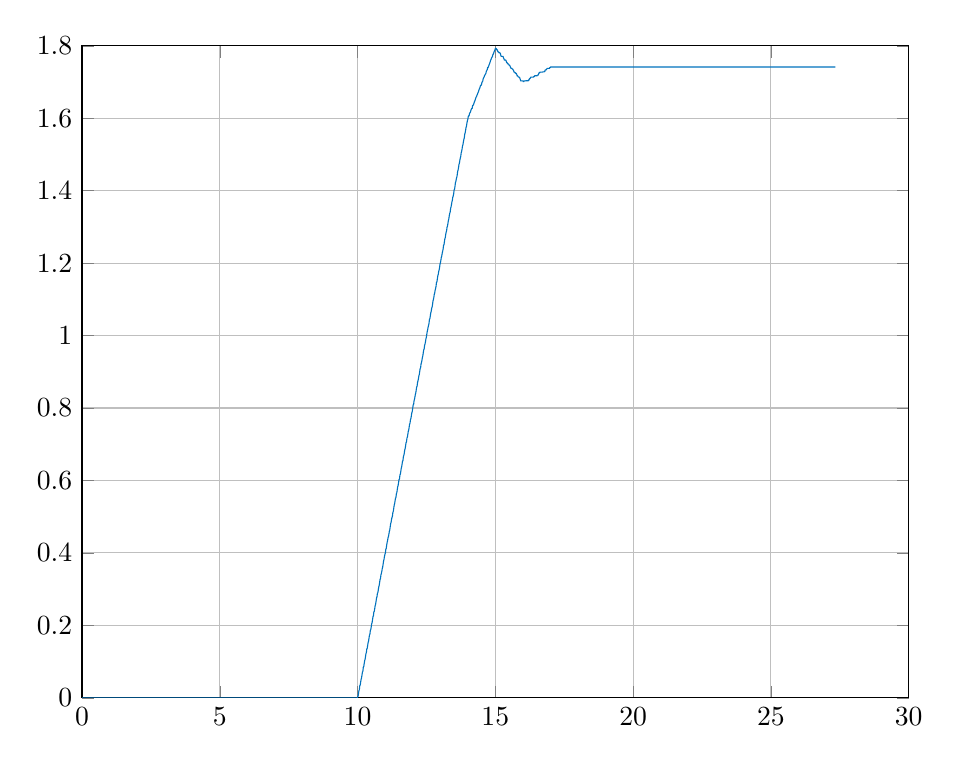
\begin{tikzpicture}

\begin{axis}[%
width=4.133in,
height=3.26in,
at={(0.693in,0.44in)},
scale only axis,
xmin=0,
xmax=30,
xmajorgrids,
ymin=0,
ymax=1.8,
ymajorgrids,
axis background/.style={fill=white}
]
\addplot [color=mycolor1,solid,forget plot]
  table[row sep=crcr]{%
0	0\\
0.017486686999999	0\\
0.0335484049999993	0\\
0.0489735169999991	0\\
0.0654204590000007	0\\
0.0807954470000006	0\\
0.095984534	0\\
0.111819789999999	0\\
0.127794892999999	0\\
0.143809515000999	0\\
0.159864158	0\\
0.176264448000001	0\\
0.191918061000001	0\\
0.208229863	0\\
0.22411426	0\\
0.240030810000001	0\\
0.255976952	0\\
0.271988863	0\\
0.288005780999999	0\\
0.303815257999999	0\\
0.319800566	0\\
0.335802525001001	0\\
0.351768663999999	0\\
0.36785526	0\\
0.383954799000001	0\\
0.399951771	0\\
0.415880339	0\\
0.431894845999999	0\\
0.447974014	0\\
0.463848232999999	0\\
0.480008339	0\\
0.495993414999001	0\\
0.511988127	0\\
0.528026147001	0\\
0.543979419999	0\\
0.560134905999999	0\\
0.576019073000001	0\\
0.591895217	0\\
0.607847277000001	0\\
0.623834802999999	0\\
0.639813487999	0\\
0.655864687999999	0\\
0.671844843	0\\
0.687894173	0\\
0.703960452998999	0\\
0.719861596999001	0\\
0.735862183	0\\
0.751862538000001	0\\
0.767889197000999	0\\
0.783981379999001	0\\
0.799994904999999	0\\
0.815962780998999	0\\
0.831992070999	0\\
0.847937220999999	0\\
0.863962322000001	0\\
0.879972584000001	0\\
0.896016072000001	0\\
0.912088118999999	0\\
0.927922307	0\\
0.944023716	0\\
0.959994168	0\\
0.975991230999	0\\
0.992029912	0\\
1.00793084	0\\
1.023850434	0\\
1.039763124	0\\
1.055901442	0\\
1.071836404	0\\
1.087869267	0\\
1.10386867	0\\
1.119916358	0\\
1.1358229	0\\
1.15185658	0\\
1.167908877	0\\
1.183846768001	0\\
1.199820039001	0\\
1.215989863	0\\
1.232047372	0\\
1.248097771	0\\
1.264938424	0\\
1.280224831001	0\\
1.295854792	0\\
1.311873158	0\\
1.327965721999	0\\
1.343997818	0\\
1.359990541	0\\
1.375953205	0\\
1.391990664	0\\
1.407983296	0\\
1.42398526	0\\
1.439988907	0\\
1.455918365999	0\\
1.471983127	0\\
1.487986744	0\\
1.50410443	0\\
1.519856507	0\\
1.536033372	0\\
1.551946803	0\\
1.568102883	0\\
1.583845648999	0\\
1.599816938	0\\
1.615792371001	0\\
1.631799331	0\\
1.647803028	0\\
1.663927058	0\\
1.680189577	0\\
1.695951467	0\\
1.711980451	0\\
1.727964409	0\\
1.744002825	0\\
1.760010982999	0\\
1.775946896	0\\
1.79184524	0\\
1.807861806	0\\
1.823847002	0\\
1.839834533	0\\
1.855985263	0\\
1.872113578	0\\
1.887788602	0\\
1.904080431	0\\
1.919815951	0\\
1.936070287999	0\\
1.95185823	0\\
1.967838134	0\\
1.983960635	0\\
2.000025140001	0\\
2.017650045	0\\
2.033143887	0\\
2.048642751	0\\
2.064027737	0\\
2.079982323	0\\
2.096419011999	0\\
2.11211212	0\\
2.127943664	0\\
2.144116339	0\\
2.1600051	0\\
2.175997858	0\\
2.191989798	0\\
2.207913897	0\\
2.22381201	0\\
2.239988593001	0\\
2.25599238	0\\
2.272004612	0\\
2.287857763001	0\\
2.303951063999	0\\
2.319942919	0\\
2.335980313	0\\
2.352239169	0\\
2.368013311	0\\
2.38401129	0\\
2.400130168	0\\
2.415943846	0\\
2.431985569	0\\
2.448257389	0\\
2.463981428001	0\\
2.479988824	0\\
2.495996796	0\\
2.512120174	0\\
2.528009412	0\\
2.543985026	0\\
2.560078320999	0\\
2.575957309	0\\
2.592038575	0\\
2.608019255	0\\
2.623982851	0\\
2.639868857001	0\\
2.655847989001	0\\
2.672064518	0\\
2.687855789	0\\
2.703825219	0\\
2.719867364	0\\
2.735848425	0\\
2.751841428	0\\
2.767796685999	0\\
2.783994127	0\\
2.799976426	0\\
2.815987054	0\\
2.831971804	0\\
2.847952003	0\\
2.864066180001	0\\
2.880101629999	0\\
2.896000037999	0\\
2.9119947	0\\
2.928207542	0\\
2.943964816	0\\
2.959980711001	0\\
2.975975097	0\\
2.991968672	0\\
3.008049589	0\\
3.025705628001	0\\
3.041302558	0\\
3.056294674	0\\
3.071707325	0\\
3.087762018	0\\
3.10588222	0\\
3.120848061	0\\
3.136017734	0\\
3.151834834	0\\
3.168017411001	0\\
3.183817157	0\\
3.199883506	0\\
3.215999618	0\\
3.231906530999	0\\
3.247868268	0\\
3.263899598999	0\\
3.279850943	0\\
3.295889188	0\\
3.311824488	0\\
3.330103953	0\\
3.34520471	0\\
3.360502328	0\\
3.376507724	0\\
3.391998727	0\\
3.407956905	0\\
3.423716052	0\\
3.439988605	0\\
3.455983166001	0\\
3.471984804	0\\
3.487860982001	0\\
3.506367524	0\\
3.521821832	0\\
3.536967627	0\\
3.552019848001	0\\
3.567876423001	0\\
3.583855765	0\\
3.600034659001	0\\
3.616012623	0\\
3.631974646	0\\
3.64803659	0\\
3.664004502	0\\
3.679872690999	0\\
3.696085323	0\\
3.712132148	0\\
3.728065185	0\\
3.743841969	0\\
3.759840189	0\\
3.775891353999	0\\
3.791852299	0\\
3.807891971	0\\
3.823991789999	0\\
3.840109428	0\\
3.855996638001	0\\
3.871925701	0\\
3.888081237001	0\\
3.903997015001	0\\
3.919870763	0\\
3.936023091999	0\\
3.951959091	0\\
3.967990361	0\\
3.983966682	0\\
3.99996206	0\\
4.017571706	0\\
4.032651770999	0\\
4.04783499	0\\
4.063893371001	0\\
4.079849379999	0\\
4.095843952001	0\\
4.111851974	0\\
4.127999232	0\\
4.14394607	0\\
4.159921162999	0\\
4.175822202999	0\\
4.191831913	0\\
4.20800091	0\\
4.223868114001	0\\
4.239983184	0\\
4.255981995	0\\
4.271850145001	0\\
4.287870174	0\\
4.303882005	0\\
4.320301229	0\\
4.335876135	0\\
4.351866602	0\\
4.367842502	0\\
4.383905609	0\\
4.399886439	0\\
4.415890207	0\\
4.431889204	0\\
4.44789114	0\\
4.463877956	0\\
4.48001681	0\\
4.495913405	0\\
4.511827202	0\\
4.527941767	0\\
4.543860352	0\\
4.559996389	0\\
4.576008185	0\\
4.591897362	0\\
4.607927595001	0\\
4.623936198	0\\
4.639968085	0\\
4.656080012	0\\
4.671823111	0\\
4.687780598	0\\
4.703962403	0\\
4.720163187	0\\
4.735872136999	0\\
4.751936527001	0\\
4.767989435	0\\
4.783966221999	0\\
4.799856497	0\\
4.815839142	0\\
4.831855848999	0\\
4.847988704	0\\
4.864022178999	0\\
4.879995537	0\\
4.895993602	0\\
4.912126157	0\\
4.928008574	0\\
4.944112568	0\\
4.959862902	0\\
4.976050516	0\\
4.992229881999	0\\
5.00798456	0\\
5.025727621	0\\
5.040911994	0\\
5.056201608	0\\
5.072061125	0\\
5.08785427	0\\
5.103860728	0\\
5.119839359	0\\
5.135849677	0\\
5.15183426	0\\
5.167928034	0\\
5.18420363	0\\
5.200012105	0\\
5.215974444	0\\
5.232035055001	0\\
5.247871685	0\\
5.263861435001	0\\
5.279974855999	0\\
5.295995893	0\\
5.312029757	0\\
5.32800208	0\\
5.343979879	0\\
5.359990474	0\\
5.377331107001	0\\
5.392508933	0\\
5.408060076	0\\
5.42388316	0\\
5.439875421	0\\
5.455980373	0\\
5.471983484	0\\
5.487966665	0\\
5.503868211001	0\\
5.51998506	0\\
5.535943665	0\\
5.551901649	0\\
5.567849605	0\\
5.583842257	0\\
5.5998659	0\\
5.615849357	0\\
5.63186656	0\\
5.647841391	0\\
5.663848662	0\\
5.679842938	0\\
5.695846786	0\\
5.711855354	0\\
5.727846343	0\\
5.74384761	0\\
5.759851372	0\\
5.775873983	0\\
5.791840385	0\\
5.807841377	0\\
5.823852486	0\\
5.839893136999	0\\
5.855842155	0\\
5.871846494	0\\
5.887839251999	0\\
5.903850416001	0\\
5.919859576	0\\
5.935856994	0\\
5.951836722	0\\
5.967980768	0\\
5.98396902	0\\
5.999988959	0\\
6.017461794	0\\
6.032542141	0\\
6.047851054	0\\
6.063789746	0\\
6.079982419	0\\
6.096028804	0\\
6.112197169	0\\
6.127987843999	0\\
6.14400659	0\\
6.160620305	0\\
6.175926587	0\\
6.191874924	0\\
6.207853971	0\\
6.223858966	0\\
6.239991129	0\\
6.255961035	0\\
6.271965805	0\\
6.287855514	0\\
6.303849871	0\\
6.319843220001	0\\
6.335992677	0\\
6.352068348	0\\
6.367996268999	0\\
6.383986896	0\\
6.399983683	0\\
6.415981171	0\\
6.432326658	0\\
6.448015282	0\\
6.463933515	0\\
6.479989165	0\\
6.495996857	0\\
6.511966723	0\\
6.527969363	0\\
6.543976087	0\\
6.560117987001	0\\
6.576019849	0\\
6.591898213001	0\\
6.60800549	0\\
6.623987182	0\\
6.639978992999	0\\
6.655979738	0\\
6.671970694	0\\
6.687890725	0\\
6.703959956	0\\
6.719903061	0\\
6.736118653	0\\
6.751990346	0\\
6.767856928	0\\
6.783841984	0\\
6.800109087	0\\
6.815839205	0\\
6.83184929	0\\
6.84785296	0\\
6.863820206	0\\
6.879848282	0\\
6.896027948	0\\
6.912100356	0\\
6.927857114	0\\
6.94401239	0\\
6.960079546	0\\
6.975990438	0\\
6.991984544	0\\
7.007979692001	0\\
7.023862178001	0\\
7.039860893001	0\\
7.055952778	0\\
7.07198731	0\\
7.08787378	0\\
7.104000367999	0\\
7.119878782	0\\
7.135843636	0\\
7.151983467	0\\
7.167992752	0\\
7.183983109	0\\
7.199993135	0\\
7.215927987	0\\
7.231990959	0\\
7.248110008	0\\
7.263994520001	0\\
7.279978317	0\\
7.29598012	0\\
7.311967852	0\\
7.327984884	0\\
7.344036841	0\\
7.359991648	0\\
7.375941638001	0\\
7.391957109	0\\
7.407991825	0\\
7.423983791001	0\\
7.440299411001	0\\
7.455997626001	0\\
7.472022897001	0\\
7.487877721	0\\
7.503976749999	0\\
7.519847844	0\\
7.535793886999	0\\
7.551727271	0\\
7.567746317	0\\
7.583805196	0\\
7.599885973	0\\
7.616033161001	0\\
7.631984665	0\\
7.648047667	0\\
7.66399407	0\\
7.679875387	0\\
7.695933044	0\\
7.711983202	0\\
7.727866161001	0\\
7.743846445	0\\
7.759983444001	0\\
7.776080985	0\\
7.792035334999	0\\
7.808116768	0\\
7.824087381	0\\
7.839867387	0\\
7.855851194	0\\
7.871966544	0\\
7.887853167	0\\
7.904021978	0\\
7.919860643001	0\\
7.935857589	0\\
7.951844027	0\\
7.967842142	0\\
7.983788231	0\\
7.999854768999	0\\
8.017226094	0\\
8.03242936	0\\
8.048033415	0\\
8.064008172	0\\
8.079984532999	0\\
8.096111955	0\\
8.111885089999	0\\
8.127851588	0\\
8.143970061	0\\
8.159966487	0\\
8.175972364001	0\\
8.191934654001	0\\
8.207990388	0\\
8.22399195	0\\
8.239967028	0\\
8.255991984	0\\
8.271880347	0\\
8.288003969	0\\
8.303895738	0\\
8.319890578	0\\
8.335951235999	0\\
8.351928202999	0\\
8.367844089	0\\
8.383987025	0\\
8.400064459	0\\
8.415987574001	0\\
8.431715610999	0\\
8.447955805001	0\\
8.46409959	0\\
8.479920212	0\\
8.49595922	0\\
8.511975155	0\\
8.527807334	0\\
8.543956756	0\\
8.559932374999	0\\
8.575968185	0\\
8.591881277	0\\
8.607929852	0\\
8.623839445	0\\
8.639833406	0\\
8.65585092	0\\
8.671917865	0\\
8.687842158	0\\
8.704015207	0\\
8.719831747	0\\
8.73599239	0\\
8.752517784001	0\\
8.768091072	0\\
8.784067327	0\\
8.800030593001	0\\
8.815993513	0\\
8.832163016	0\\
8.847965497	0\\
8.863975243	0\\
8.879895853	0\\
8.896028878001	0\\
8.911957110001	0\\
8.927983173	0\\
8.943893871001	0\\
8.959987576	0\\
8.975998971	0\\
8.992018459	0\\
9.007844945	0\\
9.025491622	0\\
9.040655504	0\\
9.05585089	0\\
9.071831285	0\\
9.087846854	0\\
9.103835227	0\\
9.119997669	0\\
9.13599966	0\\
9.151983379999	0\\
9.167836060001	0\\
9.183965129	0\\
9.199993144	0\\
9.21585087	0\\
9.231846695	0\\
9.24799586	0\\
9.263971531	0\\
9.27998909	0\\
9.296005692	0\\
9.312029775	0\\
9.327963308	0\\
9.343974773	0\\
9.359985577	0\\
9.376000405	0\\
9.392563669	0\\
9.407995697001	0\\
9.423989913	0\\
9.44008832	0\\
9.455951188	0\\
9.471966218	0\\
9.48797065	0\\
9.503844253	0\\
9.520148461	0\\
9.536045297	0\\
9.553297377	0\\
9.568767485	0\\
9.584163717	0\\
9.600208683	0\\
9.615995278	0\\
9.632013268	0\\
9.647977641	0\\
9.663963448	0\\
9.680035245	0\\
9.696007496001	0\\
9.711999838	0\\
9.727993923	0\\
9.744061065	0\\
9.760017875	0\\
9.776223054	0\\
9.792048017	0\\
9.807948174999	0\\
9.823957148999	0\\
9.839880228999	0\\
9.855805168	0\\
9.871788309	0\\
9.887849892	0\\
9.903951436	0\\
9.919780925	0\\
9.935843455	0\\
9.952036546	0\\
9.967985144	0\\
9.9840059	0\\
10.000018628	0.00195929075870865\\
10.017668344	0.00391858151741729\\
10.033358506	0.0117561525575638\\
10.048801532999	0.0199947667571325\\
10.063992134	0.0219543385127193\\
10.079961859	0.0333555692763681\\
10.096000586	0.0353148493261139\\
10.111954488	0.0431523983171564\\
10.127834398	0.0509889104837971\\
10.144004251	0.0549077008684895\\
10.159905171001	0.0627445374472635\\
10.175990233	0.0709833458951193\\
10.191972571	0.0729431078622516\\
10.207959466001	0.0843467322174817\\
10.223868092	0.0863057422184539\\
10.239857909	0.0941423127639337\\
10.255848978	0.10197826851671\\
10.271971805	0.105896708879398\\
10.287994816	0.113732857130316\\
10.303905493	0.121971725332057\\
10.319956954	0.124743095597818\\
10.335998406	0.135337214025708\\
10.351968337	0.137296220021645\\
10.367869703	0.145132204864222\\
10.383860541	0.152967286969737\\
10.399866719	0.156885334579459\\
10.415861216001	0.1651249272999\\
10.432036196	0.172959927045449\\
10.448021021	0.175732916424795\\
10.463938207	0.186327829330511\\
10.480249577001	0.188286487041644\\
10.496029262	0.196121625028826\\
10.511966554	0.203956073442876\\
10.528000834999	0.20787381101624\\
10.543984898	0.216113757068755\\
10.559988415	0.223947353347441\\
10.576110942	0.227122129784937\\
10.592011831	0.237317773852279\\
10.60798081	0.239276454543243\\
10.623987157999	0.247110894177621\\
10.639983234	0.254944534042368\\
10.655962586001	0.258861772823795\\
10.672021563	0.267101655856662\\
10.68785515	0.275344544675247\\
10.703839729	0.278515199458051\\
10.72001495	0.288307715708748\\
10.736290253	0.290265942274672\\
10.752002325	0.29809968841717\\
10.767928587	0.305932623145191\\
10.78396365	0.310256375473006\\
10.800014529001	0.318089693365345\\
10.815968128	0.326740924049042\\
10.831995911	0.329505673476397\\
10.847990132	0.339297015771402\\
10.864021076	0.343214463666393\\
10.879858917	0.349088233274227\\
10.895994147	0.356920418719696\\
10.912003758999	0.361244351780684\\
10.927812883	0.369076987908514\\
10.944089962	0.377729461849186\\
10.960012951	0.382453552557871\\
10.975967372	0.390286158368493\\
10.994437291	0.396160593342135\\
11.009855928	0.400076210326825\\
11.024862852	0.409866130263916\\
11.040363161001	0.412232397446914\\
11.055893209	0.420886334013296\\
11.071954883	0.428717367482197\\
11.08799588	0.433442924041582\\
11.103866797	0.441274687125049\\
11.119979726	0.445191290153753\\
11.135979645	0.451063850761079\\
11.152036092	0.459304041808284\\
11.167860453	0.463219477822907\\
11.183752573	0.471874482418661\\
11.199759137	0.480515918703082\\
11.215828492999	0.484431997085672\\
11.231808772	0.492262924328079\\
11.250404881999	0.498136247567149\\
11.265866270999	0.502050996717277\\
11.281521764	0.512249133016502\\
11.296757813	0.514620121737281\\
11.311903121001	0.522862654758944\\
11.327865785	0.531504900838892\\
11.343986763	0.53542025825273\\
11.359975071	0.543250541444703\\
11.376366240999	0.551079980237494\\
11.392050157	0.55303774263945\\
11.407961721	0.563235939216815\\
11.423941196	0.566019954824606\\
11.439990165	0.574255662832523\\
11.455954879	0.58249311096244\\
11.472048105001	0.586408283996973\\
11.487916396	0.594237780608164\\
11.503695352	0.602066494085029\\
11.521699371	0.604435499526949\\
11.536536236	0.61463701158548\\
11.551689432	0.617007589834535\\
11.569768705	0.625652643373812\\
11.584946473001	0.633480992617072\\
11.600190114001	0.637395581577943\\
11.615752999999	0.645224260733243\\
11.631693449999	0.653052227569402\\
11.647688898999	0.655422329080311\\
11.663683103	0.66603799155969\\
11.681889187001	0.669951134804266\\
11.697101984	0.676640493015479\\
11.712128372	0.684468105720095\\
11.727860143	0.68838243421456\\
11.743847957	0.696210298865991\\
11.759921565999	0.704450906627083\\
11.775981921	0.706824694144621\\
11.791976771	0.717024405863653\\
11.80795432	0.71939183583523\\
11.824044034	0.727627941846543\\
11.839996891	0.735454849726604\\
11.856056169	0.739368661040702\\
11.872050741	0.747195575372764\\
11.888032609	0.755436310298784\\
11.903815577	0.758226938647369\\
11.919827874	0.76801046731857\\
11.935811235	0.770787880660686\\
11.951821115999	0.778614678622068\\
11.967815132	0.786440647074948\\
11.983844497	0.790354214763538\\
11.99986148	0.79859571457446\\
12.017454397001	0.808796517979441\\
12.032719391	0.809213181143731\\
12.048030129	0.818995883055397\\
12.06400678	0.823732152751271\\
12.079982388999	0.829600778637035\\
12.095891701	0.837426022504511\\
12.111777777	0.841339068505069\\
12.127842794999	0.849580300358285\\
12.143991495	0.858242238273216\\
12.160025336	0.860199086538433\\
12.175987049	0.87039374789121\\
12.191947357	0.874718317910754\\
12.208013426	0.880586295378968\\
12.223962285	0.888410513161725\\
12.239861184	0.892739898904362\\
12.255963174999	0.900985001869094\\
12.27186019	0.90922743287563\\
12.287836821	0.911183879597191\\
12.303870627	0.921790539770876\\
12.319859446	0.925703493882202\\
12.33582852	0.931570920773396\\
12.351935486	0.939394639881869\\
12.36785407	0.94372441434851\\
12.383869876	0.95238834902311\\
12.399881065	0.960211966540132\\
12.415860973	0.962583194177171\\
12.431885087	0.972775496015762\\
12.447991928	0.976688050433576\\
12.463975985999	0.982555110315896\\
12.479967546001	0.99079579464459\\
12.49600742	0.995129574096111\\
12.512026683001	1.0033731473321\\
12.527979592	1.01119540181499\\
12.543979208	1.01593666610025\\
12.560080973	1.02375987567632\\
12.575893131	1.02767185286547\\
12.591957772001	1.03353813528736\\
12.607991342	1.04415808559281\\
12.623822784	1.0465342561868\\
12.639977123	1.05435665561113\\
12.655959401	1.06259523995848\\
12.671949513	1.06692083028304\\
12.687982597	1.07474318099976\\
12.704035315	1.07865492888785\\
12.720021768	1.08494048708576\\
12.736016075	1.0951408403407\\
12.751875165	1.09947425657462\\
12.767797132	1.10533986157871\\
12.783836501	1.11399313974728\\
12.800182779	1.11790441802295\\
12.816031766	1.12572608329139\\
12.831965990999	1.12963688876271\\
12.848031032	1.13634680570089\\
12.86399961	1.14654594711762\\
12.879938294999	1.14850037977558\\
12.895996756	1.15673996783221\\
12.912105462	1.16497631775798\\
12.92792629	1.16888674531932\\
12.943839041	1.17670761189332\\
12.959855833	1.18104017004783\\
12.976032022	1.18775260359598\\
12.99201621	1.19752792354879\\
13.007858497	1.20143889619749\\
13.023792321	1.20813870598505\\
13.039744899	1.21595827518656\\
13.05591623	1.21986843599691\\
13.071846596	1.22768854379039\\
13.087981905999	1.23244668271075\\
13.103950594	1.23873489193153\\
13.120117336	1.24850979820642\\
13.136024737	1.25088342808191\\
13.151997252	1.25912086345168\\
13.167858489	1.26693982625676\\
13.183939222	1.27084894548704\\
13.199923226	1.27951794832506\\
13.215962118	1.28580748131857\\
13.231953358	1.28971616535515\\
13.248001446	1.29948984680208\\
13.263987298001	1.30228302234755\\
13.279980055	1.31010171794896\\
13.296214871	1.31791983156148\\
13.312134383001	1.32225317590597\\
13.328006872999	1.33092451266319\\
13.343871655999	1.33678812268356\\
13.359846959	1.34069682125624\\
13.376176419	1.35089098968993\\
13.391998771	1.35521939906714\\
13.407951793	1.36108188419315\\
13.423934056999	1.3688996485314\\
13.440016056999	1.37366044974873\\
13.455928718001	1.38190498470828\\
13.47200945	1.3858145989605\\
13.487994726	1.39167585216295\\
13.503930695	1.40229023125838\\
13.520122669	1.40424412112732\\
13.535994387	1.41206062732352\\
13.552143063	1.42268657512834\\
13.567978359	1.42506765853592\\
13.583843648	1.43288473642861\\
13.599871936	1.43679336151409\\
13.615848983	1.44307799965186\\
13.632066635	1.4532691577886\\
13.648000169	1.4571780055111\\
13.663961109	1.46346567366241\\
13.679905552	1.47213896032879\\
13.695858747999	1.47604672062931\\
13.711932391	1.48386307291891\\
13.72796795	1.49014914492234\\
13.743951187001	1.49447750474113\\
13.759979856	1.50424734389641\\
13.776030564	1.50815626451194\\
13.7920226	1.51487339177463\\
13.807942248	1.52311764132488\\
13.823999681999	1.52702562351866\\
13.84001694	1.53483997816272\\
13.856214341001	1.54112679285349\\
13.872008414	1.54545610178194\\
13.887983235	1.55522421597514\\
13.903994861	1.55999141744094\\
13.919937625	1.56628126593932\\
13.936033271	1.57409541188004\\
13.951986549	1.57800240876508\\
13.967998911001	1.58624253966634\\
13.983962302	1.59252669656045\\
13.999994825	1.59643270317195\\
14.017505371001	1.60467942250916\\
14.032585284999	1.60663299166837\\
14.047964185	1.60663299166837\\
14.063867397001	1.6133536361109\\
14.080146228	1.61530645451251\\
14.095993591	1.61726002367171\\
14.111979188	1.6211688732894\\
14.127994191	1.62507488621513\\
14.143957306	1.62745417508715\\
14.159874658	1.62745417508715\\
14.175938191	1.63526903763057\\
14.191981277	1.63569236956274\\
14.207869819001	1.63764593872194\\
14.223915171	1.64155478833963\\
14.239848654	1.64546080126536\\
14.255865086	1.64741437042457\\
14.271942861	1.65175507683604\\
14.288025542	1.65566108976178\\
14.303891578	1.65847325922171\\
14.319946526	1.66042742470245\\
14.336028761	1.66433530336352\\
14.351872246	1.66628812176512\\
14.367987801999	1.67062157611789\\
14.384143343001	1.67257626025483\\
14.399955962	1.67648227318056\\
14.415984035	1.68039000782051\\
14.431957684	1.68234469195745\\
14.448025066	1.68667403681535\\
14.463973187	1.6905817714553\\
14.480037472	1.6905817714553\\
14.495865577	1.69253645559224\\
14.512023894	1.69882849079251\\
14.527988935	1.70078205995172\\
14.544015689	1.70273674408866\\
14.559991834	1.70945552279586\\
14.575987177	1.71140909195507\\
14.591970228	1.71378949580482\\
14.607939893999	1.71769685580969\\
14.623969289	1.7196496742113\\
14.640000322999	1.72160324337051\\
14.656042072	1.72355792750745\\
14.671992744001	1.72941810591392\\
14.68785877	1.7317950070053\\
14.703814629	1.73374969114224\\
14.719799759	1.73960986954871\\
14.735826303	1.73960986954871\\
14.751810757	1.74351812284486\\
14.767883837	1.74590414511939\\
14.784403879	1.74981015804513\\
14.799988823	1.75262232750506\\
14.815851666	1.75653117712274\\
14.831857779	1.76086290976129\\
14.847833027001	1.7628164789205\\
14.863882498	1.76672532853818\\
14.879853897	1.76867852306231\\
14.895881478	1.77063134146392\\
14.911957279	1.7764937602408\\
14.928018539	1.77691709217297\\
14.944133376	1.78082310509871\\
14.959996134	1.78473083973865\\
14.97601438	1.78668552387559\\
14.991969301999	1.79059153680133\\
15.007964845	1.79297755907586\\
15.025661518	1.79297755907586\\
15.040820341	1.79102293039607\\
15.056224806	1.78863750444307\\
15.071796811	1.78863750444307\\
15.08784769	1.78473149151733\\
15.103984965	1.78277633322473\\
15.120584066	1.78277633322473\\
15.136154065999	1.78082231646726\\
15.15209219	1.78082190580592\\
15.167991652	1.78039857387375\\
15.183706164001	1.77844500471454\\
15.201759735	1.77258388609347\\
15.217388007	1.77063001829735\\
15.232905603	1.77063001829735\\
15.248296016	1.77062966041186\\
15.263963767	1.77062966041186\\
15.280054823	1.77062966041186\\
15.296020414001	1.7667210383927\\
15.311987974	1.76476731979601\\
15.328046937	1.76086130687028\\
15.343970919	1.76086100199875\\
15.359881395	1.76086100199875\\
15.375884486	1.76043289514072\\
15.391968254	1.75847925123302\\
15.407997786	1.7541419682405\\
15.424042336	1.7541419682405\\
15.439856964999	1.75023595531477\\
15.456127652001	1.75023536273967\\
15.471978052	1.75023536273967\\
15.487966064	1.74828186838847\\
15.503843471	1.74632665583855\\
15.519966161	1.74589650336452\\
15.535982535	1.74394293420531\\
15.551979686	1.74003638222073\\
15.568175523999	1.73808303766406\\
15.583861907	1.73808303766406\\
15.599826639	1.73765070615208\\
15.615854448	1.73569602201514\\
15.631846093	1.73569602201514\\
15.647848268	1.73331863561924\\
15.663838434	1.73136544109511\\
15.679902148	1.72745942816937\\
15.696025843001	1.72745942816937\\
15.711890284	1.7255043232471\\
15.727964952	1.7255043232471\\
15.743914416001	1.72355120382849\\
15.760064105	1.72355084768136\\
15.775993890001	1.72116644428083\\
15.791955356	1.71726043135509\\
15.80799266	1.71725972387669\\
15.823964861	1.71530503973975\\
15.839869749	1.71335207071066\\
15.855842507	1.71335142806209\\
15.871849867999	1.71335142806209\\
15.88790435	1.71139785890288\\
15.904392189	1.70749119293392\\
15.919982515001	1.70358369039537\\
15.935988683	1.70315524256868\\
15.951957441	1.7031546545338\\
15.967857509	1.7031546545338\\
15.983846212	1.7031546545338\\
15.999962339	1.70315405616378\\
16.017517646	1.70120138862761\\
16.032688442	1.70120138862761\\
16.048149896	1.70315405616378\\
16.064113332999	1.70315405616378\\
16.080008785	1.70315405616378\\
16.095961627	1.70315405616378\\
16.112004764	1.70358250399048\\
16.127964431999	1.70358250399048\\
16.143976628	1.70358250399048\\
16.160000321	1.70358250399048\\
16.17607249	1.70358250399048\\
16.191987274	1.70358250399048\\
16.208037217	1.70553718812742\\
16.22399262	1.70553718812742\\
16.239877232	1.7094434248228\\
16.255945610999	1.7094434248228\\
16.271848865999	1.71139661934693\\
16.28784699	1.71334943774853\\
16.303847586	1.71334943774853\\
16.319818905	1.71334943774853\\
16.335847704	1.71334943774853\\
16.352030929	1.71334943774853\\
16.367970390001	1.71334943774853\\
16.383715136	1.71334943774853\\
16.399728560001	1.71530412188548\\
16.415784848001	1.71530412188548\\
16.431910035	1.71725678942165\\
16.447990225	1.71725678942165\\
16.463950805	1.71725678942165\\
16.479734909	1.71725678942165\\
16.495704999	1.71725678942165\\
16.513856678	1.71725678942165\\
16.52875146	1.71921035858086\\
16.543922847	1.71921035858086\\
16.560009081	1.71964289701055\\
16.576072243	1.72354890993628\\
16.59196082	1.72550359407322\\
16.607864129999	1.72550359407322\\
16.623845196	1.7274562616094\\
16.639820183999	1.7274562616094\\
16.655829082	1.7274562616094\\
16.671829252	1.7274562616094\\
16.687915456	1.7274562616094\\
16.703969924	1.7274562616094\\
16.719966269	1.72787959354157\\
16.735964615	1.72787959354157\\
16.751957543	1.72787959354157\\
16.767959055001	1.72787959354157\\
16.783785306	1.72983427767851\\
16.799734558999	1.72983427767851\\
16.815733957	1.73374051437389\\
16.833800629	1.73374051437389\\
16.848679415	1.73374051437389\\
16.863706291	1.73569370889802\\
16.881760272	1.73764652729963\\
16.896666697001	1.73764652729963\\
16.911775562001	1.73764652729963\\
16.927722907	1.73764652729963\\
16.943940587	1.73764652729963\\
16.959902704	1.73764652729963\\
16.975753610999	1.73960121143657\\
16.9921274	1.73960121143657\\
17.008000469	1.74155387897275\\
17.025863544	1.74155387897275\\
17.041092426	1.74155387897275\\
17.056177337	1.74155387897275\\
17.071869559	1.74155387897275\\
17.087918299	1.74155387897275\\
17.104006935	1.74155387897275\\
17.119897072999	1.74155387897275\\
17.135990688999	1.74155387897275\\
17.152013084	1.74155387897275\\
17.167959011	1.74155387897275\\
17.183838131001	1.74155387897275\\
17.199848980001	1.74155387897275\\
17.21596468	1.74155387897275\\
17.232027246	1.74155387897275\\
17.248034041	1.74155387897275\\
17.26396996	1.74155387897275\\
17.279975657	1.74155387897275\\
17.295859492	1.74155387897275\\
17.311968058	1.74155387897275\\
17.327984694	1.74155387897275\\
17.343860296	1.74155387897275\\
17.359852703	1.74155387897275\\
17.376004651	1.74155387897275\\
17.391890747	1.74155387897275\\
17.407816312	1.74155387897275\\
17.42391026	1.74155387897275\\
17.439815258001	1.74155387897275\\
17.455978096	1.74155387897275\\
17.471736298001	1.74155387897275\\
17.489935733	1.74155387897275\\
17.504925426	1.74155387897275\\
17.520689742	1.74155387897275\\
17.537219983	1.74155387897275\\
17.552052568	1.74155387897275\\
17.567695725001	1.74155387897275\\
17.585743891	1.74155387897275\\
17.600662918	1.74155387897275\\
17.616058233	1.74155387897275\\
17.631712181	1.74155387897275\\
17.649805993	1.74155387897275\\
17.6647244	1.74155387897275\\
17.679697486	1.74155387897275\\
17.697803862001	1.74155387897275\\
17.712675811	1.74155387897275\\
17.727703604	1.74155387897275\\
17.745704318	1.74155387897275\\
17.760588605	1.74155387897275\\
17.77569267	1.74155387897275\\
17.793704681	1.74155387897275\\
17.808644798	1.74155387897275\\
17.823708869	1.74155387897275\\
17.841774325	1.74155387897275\\
17.856663253	1.74155387897275\\
17.871696656	1.74155387897275\\
17.889769353	1.74155387897275\\
17.904684919	1.74155387897275\\
17.919760850001	1.74155387897275\\
17.937756297	1.74155387897275\\
17.952573419	1.74155387897275\\
17.967702661001	1.74155387897275\\
17.985722971999	1.74155387897275\\
18.00056186	1.74155387897275\\
18.017619308	1.74155387897275\\
18.03246994	1.74155387897275\\
18.047725777001	1.74155387897275\\
18.063774362001	1.74155387897275\\
18.081891108	1.74155387897275\\
18.097230375	1.74155387897275\\
18.112469846999	1.74155387897275\\
18.127907624	1.74155387897275\\
18.143765162	1.74155387897275\\
18.159796461	1.74155387897275\\
18.175803470001	1.74155387897275\\
18.193939686	1.74155387897275\\
18.207885768	1.74155387897275\\
18.223738921	1.74155387897275\\
18.239895754	1.74155387897275\\
18.255822669999	1.74155387897275\\
18.272403217	1.74155387897275\\
18.287829009	1.74155387897275\\
18.30393959	1.74155387897275\\
18.319756306	1.74155387897275\\
18.337959949001	1.74155387897275\\
18.352987810001	1.74155387897275\\
18.367927133	1.74155387897275\\
18.38382451	1.74155387897275\\
18.399720395	1.74155387897275\\
18.417809681	1.74155387897275\\
18.432670225	1.74155387897275\\
18.447838515	1.74155387897275\\
18.463791142	1.74155387897275\\
18.479975811	1.74155387897275\\
18.495888361	1.74155387897275\\
18.511961516	1.74155387897275\\
18.527858214999	1.74155387897275\\
18.543979428	1.74155387897275\\
18.559893312001	1.74155387897275\\
18.575853355999	1.74155387897275\\
18.591852267	1.74155387897275\\
18.607859628	1.74155387897275\\
18.623843606	1.74155387897275\\
18.639897752	1.74155387897275\\
18.655996613	1.74155387897275\\
18.671965885	1.74155387897275\\
18.687963403	1.74155387897275\\
18.704104852	1.74155387897275\\
18.71988154	1.74155387897275\\
18.735844577999	1.74155387897275\\
18.751749129	1.74155387897275\\
18.767761343	1.74155387897275\\
18.783830404001	1.74155387897275\\
18.799738565	1.74155387897275\\
18.815954623	1.74155387897275\\
18.832014064	1.74155387897275\\
18.847959128	1.74155387897275\\
18.863999118	1.74155387897275\\
18.879987942	1.74155387897275\\
18.896069546	1.74155387897275\\
18.912179639	1.74155387897275\\
18.927993396	1.74155387897275\\
18.943971209999	1.74155387897275\\
18.959987376001	1.74155387897275\\
18.976096762	1.74155387897275\\
18.991990816	1.74155387897275\\
19.00837016	1.74155387897275\\
19.024136915	1.74155387897275\\
19.039973013	1.74155387897275\\
19.055886366	1.74155387897275\\
19.071963731	1.74155387897275\\
19.087959921	1.74155387897275\\
19.103970785	1.74155387897275\\
19.119880388	1.74155387897275\\
19.135965801	1.74155387897275\\
19.151980433	1.74155387897275\\
19.167970291999	1.74155387897275\\
19.184376558999	1.74155387897275\\
19.200135076	1.74155387897275\\
19.215870566	1.74155387897275\\
19.231859289	1.74155387897275\\
19.247869326	1.74155387897275\\
19.266232589999	1.74155387897275\\
19.281389287	1.74155387897275\\
19.296521419999	1.74155387897275\\
19.311771995	1.74155387897275\\
19.327852117	1.74155387897275\\
19.343865992	1.74155387897275\\
19.360196094	1.74155387897275\\
19.376004529	1.74155387897275\\
19.391718386	1.74155387897275\\
19.410013238	1.74155387897275\\
19.425320156	1.74155387897275\\
19.440931054	1.74155387897275\\
19.456409150999	1.74155387897275\\
19.471845428	1.74155387897275\\
19.487843553001	1.74155387897275\\
19.503830287	1.74155387897275\\
19.519884809	1.74155387897275\\
19.535986303001	1.74155387897275\\
19.551939708	1.74155387897275\\
19.567995567	1.74155387897275\\
19.583984243	1.74155387897275\\
19.599996352	1.74155387897275\\
19.616050418	1.74155387897275\\
19.631867929	1.74155387897275\\
19.647839914999	1.74155387897275\\
19.663872558	1.74155387897275\\
19.679829223	1.74155387897275\\
19.695911589	1.74155387897275\\
19.711940884	1.74155387897275\\
19.727959892	1.74155387897275\\
19.74401462	1.74155387897275\\
19.759989056	1.74155387897275\\
19.775777585	1.74155387897275\\
19.791667472	1.74155387897275\\
19.807666350999	1.74155387897275\\
19.823674697	1.74155387897275\\
19.839739436	1.74155387897275\\
19.855661152001	1.74155387897275\\
19.871681181	1.74155387897275\\
19.887671569	1.74155387897275\\
19.905883468001	1.74155387897275\\
19.921355597	1.74155387897275\\
19.936829629	1.74155387897275\\
19.952205680001	1.74155387897275\\
19.968050162	1.74155387897275\\
19.983996735	1.74155387897275\\
20.000027001999	1.74155387897275\\
20.017910129	1.74155387897275\\
20.033451207	1.74155387897275\\
20.04868516	1.74155387897275\\
20.064084938999	1.74155387897275\\
20.079990319001	1.74155387897275\\
20.095977964999	1.74155387897275\\
20.111995218	1.74155387897275\\
20.128131526	1.74155387897275\\
20.143989683999	1.74155387897275\\
20.159978207	1.74155387897275\\
20.175972017	1.74155387897275\\
20.19198494	1.74155387897275\\
20.207866581	1.74155387897275\\
20.223800746	1.74155387897275\\
20.239961283	1.74155387897275\\
20.255979454	1.74155387897275\\
20.273507522001	1.74155387897275\\
20.287962244	1.74155387897275\\
20.304000609	1.74155387897275\\
20.320096219	1.74155387897275\\
20.335855664	1.74155387897275\\
20.351874084001	1.74155387897275\\
20.367978149	1.74155387897275\\
20.383783703	1.74155387897275\\
20.401827682	1.74155387897275\\
20.416707212	1.74155387897275\\
20.431880138	1.74155387897275\\
20.447930686	1.74155387897275\\
20.463844295	1.74155387897275\\
20.479835183	1.74155387897275\\
20.495845706	1.74155387897275\\
20.511921096	1.74155387897275\\
20.527785999	1.74155387897275\\
20.543962663	1.74155387897275\\
20.559966256	1.74155387897275\\
20.57593645	1.74155387897275\\
20.591972908	1.74155387897275\\
20.60797373	1.74155387897275\\
20.624033890001	1.74155387897275\\
20.639914969	1.74155387897275\\
20.655931386	1.74155387897275\\
20.671876701	1.74155387897275\\
20.687855126	1.74155387897275\\
20.70385735	1.74155387897275\\
20.719855615	1.74155387897275\\
20.735844088001	1.74155387897275\\
20.751865796001	1.74155387897275\\
20.767877857001	1.74155387897275\\
20.783880227	1.74155387897275\\
20.799809681	1.74155387897275\\
20.815843176	1.74155387897275\\
20.831861903	1.74155387897275\\
20.847868502	1.74155387897275\\
20.863698093999	1.74155387897275\\
20.879664898	1.74155387897275\\
20.895660773999	1.74155387897275\\
20.913927903	1.74155387897275\\
20.928990644	1.74155387897275\\
20.944062575	1.74155387897275\\
20.959883113	1.74155387897275\\
20.97596645	1.74155387897275\\
20.991900109	1.74155387897275\\
21.007984704999	1.74155387897275\\
21.025902839	1.74155387897275\\
21.041257822	1.74155387897275\\
21.056469720001	1.74155387897275\\
21.07183648	1.74155387897275\\
21.087887495	1.74155387897275\\
21.103923209999	1.74155387897275\\
21.119849066	1.74155387897275\\
21.135845562	1.74155387897275\\
21.151873369001	1.74155387897275\\
21.167882845	1.74155387897275\\
21.183990051	1.74155387897275\\
21.199931513	1.74155387897275\\
21.215854532	1.74155387897275\\
21.231965543	1.74155387897275\\
21.247999834	1.74155387897275\\
21.263992527	1.74155387897275\\
21.280046296	1.74155387897275\\
21.295954388999	1.74155387897275\\
21.31197509	1.74155387897275\\
21.327860519	1.74155387897275\\
21.343964478	1.74155387897275\\
21.359964341999	1.74155387897275\\
21.375853001001	1.74155387897275\\
21.391722498	1.74155387897275\\
21.409801405999	1.74155387897275\\
21.424854324	1.74155387897275\\
21.440132298	1.74155387897275\\
21.457224084999	1.74155387897275\\
21.47238687	1.74155387897275\\
21.487794565999	1.74155387897275\\
21.50639076	1.74155387897275\\
21.520904986	1.74155387897275\\
21.537640012	1.74155387897275\\
21.553210533	1.74155387897275\\
21.568698989	1.74155387897275\\
21.584111617	1.74155387897275\\
21.599913658	1.74155387897275\\
21.615960864	1.74155387897275\\
21.631866133	1.74155387897275\\
21.64799785	1.74155387897275\\
21.66396042	1.74155387897275\\
21.679854032999	1.74155387897275\\
21.695834422	1.74155387897275\\
21.711839172	1.74155387897275\\
21.727991546	1.74155387897275\\
21.743981202	1.74155387897275\\
21.760266533	1.74155387897275\\
21.775728627	1.74155387897275\\
21.79166907	1.74155387897275\\
21.807703426	1.74155387897275\\
21.82365321	1.74155387897275\\
21.839691584	1.74155387897275\\
21.855711001	1.74155387897275\\
21.871678298001	1.74155387897275\\
21.887871279	1.74155387897275\\
21.903849634	1.74155387897275\\
21.919842863	1.74155387897275\\
21.935853396	1.74155387897275\\
21.95184474	1.74155387897275\\
21.967850421999	1.74155387897275\\
21.983850281	1.74155387897275\\
21.999823795	1.74155387897275\\
22.017495987	1.74155387897275\\
22.03191975	1.74155387897275\\
22.047981485	1.74155387897275\\
22.063968441	1.74155387897275\\
22.080108298001	1.74155387897275\\
22.095915235999	1.74155387897275\\
22.112149631	1.74155387897275\\
22.127996351	1.74155387897275\\
22.143998432	1.74155387897275\\
22.160005898	1.74155387897275\\
22.175971629	1.74155387897275\\
22.191963725	1.74155387897275\\
22.208002041	1.74155387897275\\
22.223968118	1.74155387897275\\
22.239855602	1.74155387897275\\
22.255841239001	1.74155387897275\\
22.271785287	1.74155387897275\\
22.287943238	1.74155387897275\\
22.303816485	1.74155387897275\\
22.319953289	1.74155387897275\\
22.335923832	1.74155387897275\\
22.351964251	1.74155387897275\\
22.36806757	1.74155387897275\\
22.383728051	1.74155387897275\\
22.399718245	1.74155387897275\\
22.415694535	1.74155387897275\\
22.431730779001	1.74155387897275\\
22.44796406	1.74155387897275\\
22.463968605	1.74155387897275\\
22.479915914	1.74155387897275\\
22.49599841	1.74155387897275\\
22.511748671	1.74155387897275\\
22.527983249	1.74155387897275\\
22.544010029001	1.74155387897275\\
22.560114584	1.74155387897275\\
22.576016922	1.74155387897275\\
22.59198543	1.74155387897275\\
22.607726787999	1.74155387897275\\
22.624040919	1.74155387897275\\
22.64016106	1.74155387897275\\
22.655967766	1.74155387897275\\
22.671964652999	1.74155387897275\\
22.687973186	1.74155387897275\\
22.703870643	1.74155387897275\\
22.719710519	1.74155387897275\\
22.73780368	1.74155387897275\\
22.753066409001	1.74155387897275\\
22.768305207	1.74155387897275\\
22.784014344	1.74155387897275\\
22.799921596999	1.74155387897275\\
22.815855126	1.74155387897275\\
22.831852514	1.74155387897275\\
22.847851576	1.74155387897275\\
22.86401462	1.74155387897275\\
22.87995112	1.74155387897275\\
22.896080861	1.74155387897275\\
22.912108043	1.74155387897275\\
22.927997557	1.74155387897275\\
22.943997846	1.74155387897275\\
22.959998867999	1.74155387897275\\
22.976002134	1.74155387897275\\
22.991997306999	1.74155387897275\\
23.008009695	1.74155387897275\\
23.025560262	1.74155387897275\\
23.041022205	1.74155387897275\\
23.05635921	1.74155387897275\\
23.071822348	1.74155387897275\\
23.087827122999	1.74155387897275\\
23.103740474	1.74155387897275\\
23.11988083	1.74155387897275\\
23.135953891	1.74155387897275\\
23.152258669999	1.74155387897275\\
23.168181108	1.74155387897275\\
23.183962366	1.74155387897275\\
23.200022256001	1.74155387897275\\
23.215963978	1.74155387897275\\
23.2319697	1.74155387897275\\
23.247840767	1.74155387897275\\
23.26604081	1.74155387897275\\
23.28108139	1.74155387897275\\
23.296191019	1.74155387897275\\
23.312712297	1.74155387897275\\
23.327843649	1.74155387897275\\
23.343835054	1.74155387897275\\
23.359856100001	1.74155387897275\\
23.375945031	1.74155387897275\\
23.391739945	1.74155387897275\\
23.409744897001	1.74155387897275\\
23.424652053999	1.74155387897275\\
23.439907514	1.74155387897275\\
23.45813677	1.74155387897275\\
23.473112629999	1.74155387897275\\
23.488438181	1.74155387897275\\
23.503797264	1.74155387897275\\
23.519696914	1.74155387897275\\
23.53580193	1.74155387897275\\
23.553014820999	1.74155387897275\\
23.567958912	1.74155387897275\\
23.583806782	1.74155387897275\\
23.599808368	1.74155387897275\\
23.615953561	1.74155387897275\\
23.631741293	1.74155387897275\\
23.647770037999	1.74155387897275\\
23.663888720001	1.74155387897275\\
23.679743401	1.74155387897275\\
23.695864564	1.74155387897275\\
23.711993758	1.74155387897275\\
23.727962369	1.74155387897275\\
23.743994296001	1.74155387897275\\
23.759925959	1.74155387897275\\
23.775739219	1.74155387897275\\
23.791970297	1.74155387897275\\
23.807762145	1.74155387897275\\
23.823687945	1.74155387897275\\
23.839681058	1.74155387897275\\
23.855673759	1.74155387897275\\
23.871688529	1.74155387897275\\
23.887694525	1.74155387897275\\
23.903762181	1.74155387897275\\
23.919760238	1.74155387897275\\
23.935905431999	1.74155387897275\\
23.951835673	1.74155387897275\\
23.967754408	1.74155387897275\\
23.983712933	1.74155387897275\\
23.999826187	1.74155387897275\\
24.017461093001	1.74155387897275\\
24.032018996	1.74155387897275\\
24.047880739001	1.74155387897275\\
24.063862407	1.74155387897275\\
24.079840355	1.74155387897275\\
24.095876487	1.74155387897275\\
24.11201766	1.74155387897275\\
24.128030168	1.74155387897275\\
24.143982063	1.74155387897275\\
24.159971739001	1.74155387897275\\
24.175993993	1.74155387897275\\
24.191991386	1.74155387897275\\
24.208112159001	1.74155387897275\\
24.223957794	1.74155387897275\\
24.239990095	1.74155387897275\\
24.255930223	1.74155387897275\\
24.271741556	1.74155387897275\\
24.28798474	1.74155387897275\\
24.304016730999	1.74155387897275\\
24.319983619999	1.74155387897275\\
24.33586913	1.74155387897275\\
24.35198441	1.74155387897275\\
24.367977088001	1.74155387897275\\
24.384684484	1.74155387897275\\
24.400084379	1.74155387897275\\
24.415795622999	1.74155387897275\\
24.43189798	1.74155387897275\\
24.447777122	1.74155387897275\\
24.463730853	1.74155387897275\\
24.479777289999	1.74155387897275\\
24.495692033	1.74155387897275\\
24.511714076	1.74155387897275\\
24.527700905999	1.74155387897275\\
24.543761357	1.74155387897275\\
24.559748292	1.74155387897275\\
24.575687541001	1.74155387897275\\
24.591663573	1.74155387897275\\
24.607687268999	1.74155387897275\\
24.623851097	1.74155387897275\\
24.639846024	1.74155387897275\\
24.65587553	1.74155387897275\\
24.671988616	1.74155387897275\\
24.688044977	1.74155387897275\\
24.704549815	1.74155387897275\\
24.72012457	1.74155387897275\\
24.735984798	1.74155387897275\\
24.751982823	1.74155387897275\\
24.768001328	1.74155387897275\\
24.783917157	1.74155387897275\\
24.799991544	1.74155387897275\\
24.815991488	1.74155387897275\\
24.832020723001	1.74155387897275\\
24.848141336	1.74155387897275\\
24.863998782	1.74155387897275\\
24.880006338	1.74155387897275\\
24.895971212	1.74155387897275\\
24.912015707	1.74155387897275\\
24.927964555	1.74155387897275\\
24.943963808	1.74155387897275\\
24.960144416001	1.74155387897275\\
24.975984608	1.74155387897275\\
24.991999556	1.74155387897275\\
25.007854456	1.74155387897275\\
25.025772869	1.74155387897275\\
25.04119089	1.74155387897275\\
25.056365651	1.74155387897275\\
25.071863503001	1.74155387897275\\
25.08800786	1.74155387897275\\
25.103860268	1.74155387897275\\
25.11999579	1.74155387897275\\
25.13604065	1.74155387897275\\
25.151987845001	1.74155387897275\\
25.167845115	1.74155387897275\\
25.183959609	1.74155387897275\\
25.200025918	1.74155387897275\\
25.216330923001	1.74155387897275\\
25.231994735	1.74155387897275\\
25.247992189	1.74155387897275\\
25.264027878001	1.74155387897275\\
25.279901787	1.74155387897275\\
25.295925901	1.74155387897275\\
25.312013548	1.74155387897275\\
25.327854707	1.74155387897275\\
25.343968153	1.74155387897275\\
25.359824008	1.74155387897275\\
25.375949599	1.74155387897275\\
25.391853198	1.74155387897275\\
25.407690597	1.74155387897275\\
25.425880655	1.74155387897275\\
25.441234381001	1.74155387897275\\
25.456417394	1.74155387897275\\
25.47195486	1.74155387897275\\
25.4878848	1.74155387897275\\
25.503820850001	1.74155387897275\\
25.519921968001	1.74155387897275\\
25.5358883	1.74155387897275\\
25.551989445999	1.74155387897275\\
25.568017842	1.74155387897275\\
25.583804766	1.74155387897275\\
25.599739006	1.74155387897275\\
25.61585935	1.74155387897275\\
25.631858256	1.74155387897275\\
25.647846484	1.74155387897275\\
25.663844183	1.74155387897275\\
25.679842127	1.74155387897275\\
25.695840973	1.74155387897275\\
25.711866054	1.74155387897275\\
25.727867361	1.74155387897275\\
25.743864439	1.74155387897275\\
25.759854626	1.74155387897275\\
25.775780473001	1.74155387897275\\
25.791849232	1.74155387897275\\
25.807850869	1.74155387897275\\
25.823884309	1.74155387897275\\
25.839829657	1.74155387897275\\
25.855857938	1.74155387897275\\
25.871753761	1.74155387897275\\
25.887725711001	1.74155387897275\\
25.903740574	1.74155387897275\\
25.921961381	1.74155387897275\\
25.93680253	1.74155387897275\\
25.951820852	1.74155387897275\\
25.967797629	1.74155387897275\\
25.983803997	1.74155387897275\\
25.999803284	1.74155387897275\\
26.017121259	1.74155387897275\\
26.032117612	1.74155387897275\\
26.047852739	1.74155387897275\\
26.063798024	1.74155387897275\\
26.079965101	1.74155387897275\\
26.095988363	1.74155387897275\\
26.111981692001	1.74155387897275\\
26.127945795	1.74155387897275\\
26.144018107	1.74155387897275\\
26.159883035	1.74155387897275\\
26.175967531	1.74155387897275\\
26.191985513001	1.74155387897275\\
26.208027891	1.74155387897275\\
26.223967312	1.74155387897275\\
26.239971215	1.74155387897275\\
26.256012709	1.74155387897275\\
26.271758344	1.74155387897275\\
26.289881725001	1.74155387897275\\
26.305306942	1.74155387897275\\
26.320806055	1.74155387897275\\
26.336526835	1.74155387897275\\
26.352012132	1.74155387897275\\
26.367965319	1.74155387897275\\
26.384006381	1.74155387897275\\
26.399963017	1.74155387897275\\
26.415974176	1.74155387897275\\
26.431964175	1.74155387897275\\
26.447919538	1.74155387897275\\
26.463798859	1.74155387897275\\
26.479698734	1.74155387897275\\
26.495681731	1.74155387897275\\
26.511849604	1.74155387897275\\
26.52776905	1.74155387897275\\
26.543976905	1.74155387897275\\
26.559962596	1.74155387897275\\
26.576080086001	1.74155387897275\\
26.591903085	1.74155387897275\\
26.607889167	1.74155387897275\\
26.623848394	1.74155387897275\\
26.639885256	1.74155387897275\\
26.655958220001	1.74155387897275\\
26.671989731	1.74155387897275\\
26.688016245	1.74155387897275\\
26.703957376	1.74155387897275\\
26.720076129	1.74155387897275\\
26.736029407	1.74155387897275\\
26.751986247999	1.74155387897275\\
26.76785008	1.74155387897275\\
26.783782284	1.74155387897275\\
26.801824742	1.74155387897275\\
26.817015562	1.74155387897275\\
26.832492033	1.74155387897275\\
26.848039768999	1.74155387897275\\
26.864029785	1.74155387897275\\
26.879913294	1.74155387897275\\
26.895715096	1.74155387897275\\
26.913902128001	1.74155387897275\\
26.928905751	1.74155387897275\\
26.944197445	1.74155387897275\\
26.960051779	1.74155387897275\\
26.975871148999	1.74155387897275\\
26.991853092	1.74155387897275\\
27.007802832	1.74155387897275\\
27.02387022	1.74155387897275\\
27.039890388	1.74155387897275\\
27.055957242999	1.74155387897275\\
27.071957764	1.74155387897275\\
27.088081147001	1.74155387897275\\
27.103997622	1.74155387897275\\
27.119972469	1.74155387897275\\
27.135985398	1.74155387897275\\
27.152004069	1.74155387897275\\
27.167988909	1.74155387897275\\
27.183846115	1.74155387897275\\
27.199963138	1.74155387897275\\
27.215959795	1.74155387897275\\
27.231892596999	1.74155387897275\\
27.24801805	1.74155387897275\\
27.263894164	1.74155387897275\\
27.279719826	1.74155387897275\\
27.295861843	1.74155387897275\\
27.311793018	1.74155387897275\\
27.327998978	1.74155387897275\\
27.344027511	1.74155387897275\\
};
\end{axis}
\end{tikzpicture}%}
      \caption{The error in displacement of the robot over time for
        $(K_{\Psi}^R, K_{\omega}^T) \equiv (0.2 K_{\Psi, max}^R, 0.75 K_{\omega, max}^T)$}
      \label{fig:19_8_distance}
    \end{figure}
  \end{minipage}
  \hfill
  \begin{minipage}{0.45\linewidth}
    \begin{figure}[H]
      \scalebox{0.6}{% This file was created by matlab2tikz.
%
%The latest updates can be retrieved from
%  http://www.mathworks.com/matlabcentral/fileexchange/22022-matlab2tikz-matlab2tikz
%where you can also make suggestions and rate matlab2tikz.
%
\definecolor{mycolor1}{rgb}{0.00000,0.44700,0.74100}%
%
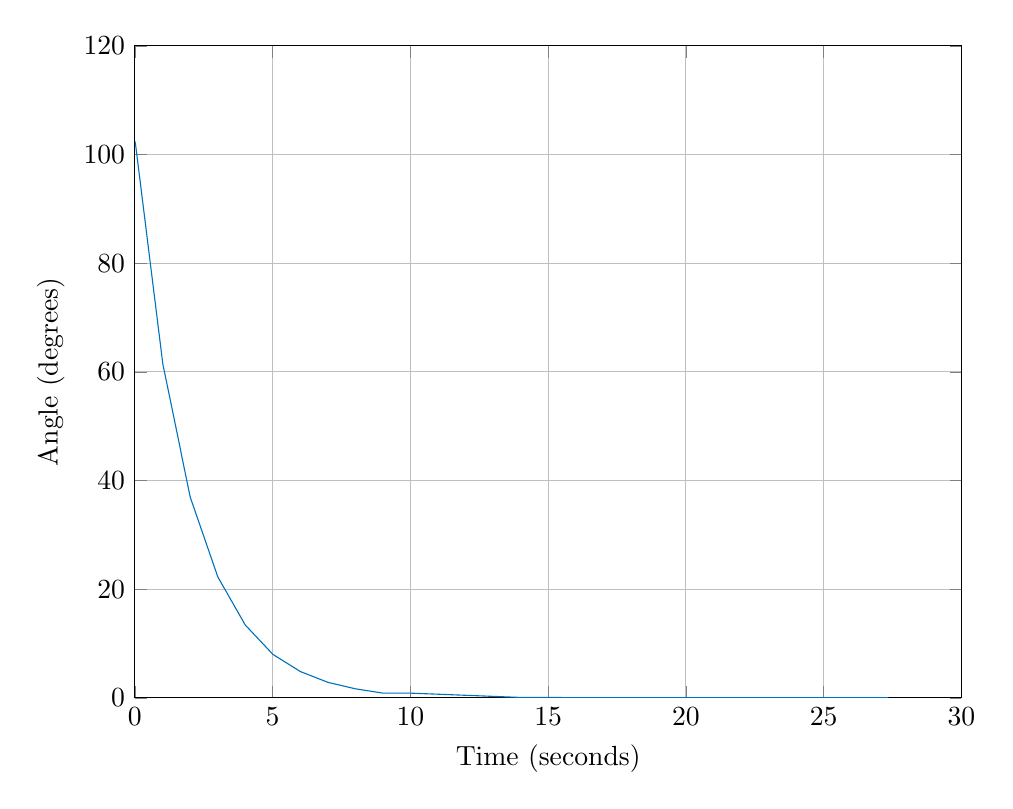
\begin{tikzpicture}

\begin{axis}[%
width=4.133in,
height=3.26in,
at={(0.693in,0.44in)},
scale only axis,
xmin=0,
xmax=30,
xmajorgrids,
xlabel={Time (seconds)},
ymin=0,
ymax=120,
ymajorgrids,
ylabel={Angle (degrees)},
axis background/.style={fill=white}
]
\addplot [color=mycolor1,solid,forget plot]
  table[row sep=crcr]{%
0	102.4204\\
0.017486686999999	102.0764\\
0.0335484049999993	101.5204\\
0.0489735169999991	100.8684\\
0.0654204590000007	100.2164\\
0.0807954470000006	99.5864\\
0.095984534	98.9524\\
0.111819789999999	98.3164\\
0.127794892999999	97.6704\\
0.143809515000999	96.9884\\
0.159864158	96.3404\\
0.176264448000001	95.6824\\
0.191918061000001	95.0424\\
0.208229863	94.3924\\
0.22411426	93.7404\\
0.240030810000001	93.0884\\
0.255976952	92.4244\\
0.271988863	91.7784\\
0.288005780999999	91.1324\\
0.303815257999999	90.4804\\
0.319800566	89.8204\\
0.335802525001001	89.1724\\
0.351768663999999	88.5224\\
0.36785526	87.8644\\
0.383954799000001	87.2124\\
0.399951771	86.5604\\
0.415880339	85.9044\\
0.431894845999999	85.2524\\
0.447974014	84.5964\\
0.463848232999999	83.9444\\
0.480008339	83.2904\\
0.495993414999001	82.6424\\
0.511988127	81.9884\\
0.528026147001	81.3044\\
0.543979419999	80.6604\\
0.560134905999999	80.0144\\
0.576019073000001	79.3664\\
0.591895217	78.7164\\
0.607847277000001	78.0684\\
0.623834802999999	77.4204\\
0.639813487999	76.7684\\
0.655864687999999	76.1144\\
0.671844843	75.4464\\
0.687894173	74.8024\\
0.703960452998999	74.1524\\
0.719861596999001	73.5004\\
0.735862183	72.8444\\
0.751862538000001	72.1984\\
0.767889197000999	71.5404\\
0.783981379999001	70.8804\\
0.799994904999999	70.2244\\
0.815962780998999	69.5724\\
0.831992070999	68.9244\\
0.847937220999999	68.2684\\
0.863962322000001	67.6104\\
0.879972584000001	66.9644\\
0.896016072000001	66.3124\\
0.912088118999999	65.6624\\
0.927922307	65.0024\\
0.944023716	64.3504\\
0.959994168	63.6924\\
0.975991230999	63.0464\\
0.992029912	62.3884\\
1.00793084	61.7084\\
1.023850434	61.1864\\
1.039763124	60.8124\\
1.055901442	60.4364\\
1.071836404	60.0384\\
1.087869267	59.6484\\
1.10386867	59.2424\\
1.119916358	58.8524\\
1.1358229	58.4684\\
1.15185658	58.0844\\
1.167908877	57.6904\\
1.183846768001	57.3004\\
1.199820039001	56.9044\\
1.215989863	56.5104\\
1.232047372	56.1184\\
1.248097771	55.7264\\
1.264938424	55.3264\\
1.280224831001	54.9384\\
1.295854792	54.5524\\
1.311873158	54.1604\\
1.327965721999	53.7644\\
1.343997818	53.3684\\
1.359990541	52.9744\\
1.375953205	52.5824\\
1.391990664	52.1884\\
1.407983296	51.7924\\
1.42398526	51.3964\\
1.439988907	51.0044\\
1.455918365999	50.6124\\
1.471983127	50.2244\\
1.487986744	49.8284\\
1.50410443	49.4324\\
1.519856507	49.0364\\
1.536033372	48.6504\\
1.551946803	48.2584\\
1.568102883	47.8624\\
1.583845648999	47.4664\\
1.599816938	47.0744\\
1.615792371001	46.6844\\
1.631799331	46.2924\\
1.647803028	45.8964\\
1.663927058	45.5064\\
1.680189577	45.0044\\
1.695951467	44.6164\\
1.711980451	44.2304\\
1.727964409	43.8364\\
1.744002825	43.4424\\
1.760010982999	43.0484\\
1.775946896	42.6504\\
1.79184524	42.2644\\
1.807861806	41.8704\\
1.823847002	41.4804\\
1.839834533	41.0844\\
1.855985263	40.6864\\
1.872113578	40.2984\\
1.887788602	39.9044\\
1.904080431	39.5144\\
1.919815951	39.1184\\
1.936070287999	38.7264\\
1.95185823	38.3324\\
1.967838134	37.9364\\
1.983960635	37.5464\\
2.000025140001	37.1644\\
2.017650045	36.8024\\
2.033143887	36.5844\\
2.048642751	36.3584\\
2.064027737	36.1244\\
2.079982323	35.9004\\
2.096419011999	35.6684\\
2.11211212	35.4264\\
2.127943664	35.1964\\
2.144116339	34.9644\\
2.1600051	34.7304\\
2.175997858	34.4924\\
2.191989798	34.2584\\
2.207913897	34.0164\\
2.22381201	33.7864\\
2.239988593001	33.5544\\
2.25599238	33.3124\\
2.272004612	33.0704\\
2.287857763001	32.8404\\
2.303951063999	32.6084\\
2.319942919	32.3804\\
2.335980313	32.1444\\
2.352239169	31.9104\\
2.368013311	31.6744\\
2.38401129	31.4404\\
2.400130168	31.2044\\
2.415943846	30.9704\\
2.431985569	30.7324\\
2.448257389	30.5024\\
2.463981428001	30.2644\\
2.479988824	30.0384\\
2.495996796	29.7984\\
2.512120174	29.5624\\
2.528009412	29.3284\\
2.543985026	29.0944\\
2.560078320999	28.8584\\
2.575957309	28.6264\\
2.592038575	28.3924\\
2.608019255	28.1584\\
2.623982851	27.9204\\
2.639868857001	27.6864\\
2.655847989001	27.4544\\
2.672064518	27.2224\\
2.687855789	26.9844\\
2.703825219	26.7484\\
2.719867364	26.5164\\
2.735848425	26.2824\\
2.751841428	26.0484\\
2.767796685999	25.8104\\
2.783994127	25.5784\\
2.799976426	25.3444\\
2.815987054	25.1044\\
2.831971804	24.8704\\
2.847952003	24.6364\\
2.864066180001	24.4044\\
2.880101629999	24.1704\\
2.896000037999	23.9324\\
2.9119947	23.7004\\
2.928207542	23.4644\\
2.943964816	23.2224\\
2.959980711001	22.9904\\
2.975975097	22.7544\\
2.991968672	22.5244\\
3.008049589	22.2904\\
3.025705628001	22.1144\\
3.041302558	21.9724\\
3.056294674	21.8384\\
3.071707325	21.7024\\
3.087762018	21.5644\\
3.10588222	21.4184\\
3.120848061	21.2764\\
3.136017734	21.1364\\
3.151834834	20.9944\\
3.168017411001	20.8504\\
3.183817157	20.7104\\
3.199883506	20.5684\\
3.215999618	20.4284\\
3.231906530999	20.2824\\
3.247868268	20.1444\\
3.263899598999	20.0024\\
3.279850943	19.8624\\
3.295889188	19.7204\\
3.311824488	19.5784\\
3.330103953	19.4284\\
3.34520471	19.2884\\
3.360502328	19.1444\\
3.376507724	19.0044\\
3.391998727	18.8624\\
3.407956905	18.7204\\
3.423716052	18.5824\\
3.439988605	18.4344\\
3.455983166001	18.2924\\
3.471984804	18.1484\\
3.487860982001	18.0104\\
3.506367524	17.8664\\
3.521821832	17.7244\\
3.536967627	17.5824\\
3.552019848001	17.4404\\
3.567876423001	17.3044\\
3.583855765	17.1604\\
3.600034659001	17.0184\\
3.616012623	16.8724\\
3.631974646	16.7324\\
3.64803659	16.5904\\
3.664004502	16.4504\\
3.679872690999	16.3044\\
3.696085323	16.1644\\
3.712132148	16.0224\\
3.728065185	15.8824\\
3.743841969	15.7384\\
3.759840189	15.5924\\
3.775891353999	15.4504\\
3.791852299	15.3104\\
3.807891971	15.1704\\
3.823991789999	15.0284\\
3.840109428	14.8844\\
3.855996638001	14.7464\\
3.871925701	14.6024\\
3.888081237001	14.4604\\
3.903997015001	14.3184\\
3.919870763	14.1784\\
3.936023091999	14.0344\\
3.951959091	13.8904\\
3.967990361	13.7504\\
3.983966682	13.6104\\
3.99996206	13.4704\\
4.017571706	13.3424\\
4.032651770999	13.2604\\
4.04783499	13.1764\\
4.063893371001	13.0944\\
4.079849379999	13.0084\\
4.095843952001	12.9224\\
4.111851974	12.8344\\
4.127999232	12.7484\\
4.14394607	12.6604\\
4.159921162999	12.5764\\
4.175822202999	12.4884\\
4.191831913	12.4024\\
4.20800091	12.3144\\
4.223868114001	12.2324\\
4.239983184	12.1464\\
4.255981995	12.0564\\
4.271850145001	11.9724\\
4.287870174	11.8844\\
4.303882005	11.8004\\
4.320301229	11.7124\\
4.335876135	11.6264\\
4.351866602	11.5424\\
4.367842502	11.4544\\
4.383905609	11.3684\\
4.399886439	11.2824\\
4.415890207	11.1984\\
4.431889204	11.1084\\
4.44789114	11.0224\\
4.463877956	10.9384\\
4.48001681	10.8504\\
4.495913405	10.7644\\
4.511827202	10.6784\\
4.527941767	10.5924\\
4.543860352	10.5044\\
4.559996389	10.4164\\
4.576008185	10.3324\\
4.591897362	10.2464\\
4.607927595001	10.1604\\
4.623936198	10.0744\\
4.639968085	9.9884\\
4.656080012	9.90239999999999\\
4.671823111	9.81439999999999\\
4.687780598	9.7304\\
4.703962403	9.64239999999999\\
4.720163187	9.55839999999999\\
4.735872136999	9.47040000000001\\
4.751936527001	9.38639999999998\\
4.767989435	9.29639999999999\\
4.783966221999	9.21040000000001\\
4.799856497	9.12239999999998\\
4.815839142	9.03639999999999\\
4.831855848999	8.95039999999999\\
4.847988704	8.86839999999999\\
4.864022178999	8.7804\\
4.879995537	8.69239999999999\\
4.895993602	8.60639999999998\\
4.912126157	8.52239999999999\\
4.928008574	8.43640000000001\\
4.944112568	8.3484\\
4.959862902	8.25839999999999\\
4.976050516	8.17439999999999\\
4.992229881999	8.0904\\
5.00798456	8.0044\\
5.025727621	7.9404\\
5.040911994	7.89439999999999\\
5.056201608	7.84439999999999\\
5.072061125	7.79239999999999\\
5.08785427	7.74239999999999\\
5.103860728	7.6944\\
5.119839359	7.64239999999999\\
5.135849677	7.5924\\
5.15183426	7.54239999999999\\
5.167928034	7.49239999999999\\
5.18420363	7.4404\\
5.200012105	7.3884\\
5.215974444	7.33840000000001\\
5.232035055001	7.28639999999999\\
5.247871685	7.23439999999999\\
5.263861435001	7.1844\\
5.279974855999	7.1344\\
5.295995893	7.08239999999999\\
5.312029757	7.0324\\
5.32800208	6.9824\\
5.343979879	6.9344\\
5.359990474	6.8844\\
5.377331107001	6.8304\\
5.392508933	6.7804\\
5.408060076	6.7304\\
5.42388316	6.6784\\
5.439875421	6.62439999999999\\
5.455980373	6.5744\\
5.471983484	6.5264\\
5.487966665	6.47439999999999\\
5.503868211001	6.4264\\
5.51998506	6.37439999999998\\
5.535943665	6.3244\\
5.551901649	6.2744\\
5.567849605	6.22439999999999\\
5.583842257	6.17440000000001\\
5.5998659	6.12439999999998\\
5.615849357	6.07039999999999\\
5.63186656	6.0164\\
5.647841391	5.96639999999999\\
5.663848662	5.91639999999998\\
5.679842938	5.86639999999998\\
5.695846786	5.8164\\
5.711855354	5.76439999999999\\
5.727846343	5.7144\\
5.74384761	5.66439999999999\\
5.759851372	5.61439999999999\\
5.775873983	5.56440000000001\\
5.791840385	5.51439999999999\\
5.807841377	5.4644\\
5.823852486	5.41239999999999\\
5.839893136999	5.3604\\
5.855842155	5.31039999999999\\
5.871846494	5.25840000000001\\
5.887839251999	5.20840000000001\\
5.903850416001	5.1544\\
5.919859576	5.10439999999998\\
5.935856994	5.0544\\
5.951836722	5.0044\\
5.967980768	4.95440000000001\\
5.98396902	4.9044\\
5.999988959	4.85439999999998\\
6.017461794	4.80839999999999\\
6.032542141	4.7784\\
6.047851054	4.74839999999998\\
6.063789746	4.7184\\
6.079982419	4.68639999999999\\
6.096028804	4.6524\\
6.112197169	4.62239999999998\\
6.127987843999	4.5904\\
6.14400659	4.55839999999999\\
6.160620305	4.5284\\
6.175926587	4.49639999999998\\
6.191874924	4.4624\\
6.207853971	4.43039999999999\\
6.223858966	4.4004\\
6.239991129	4.36839999999998\\
6.255961035	4.33840000000001\\
6.271965805	4.3044\\
6.287855514	4.2724\\
6.303849871	4.24039999999999\\
6.319843220001	4.21040000000001\\
6.335992677	4.17639999999999\\
6.352068348	4.14439999999999\\
6.367996268999	4.11239999999999\\
6.383986896	4.08239999999999\\
6.399983683	4.0504\\
6.415981171	4.02040000000001\\
6.432326658	3.98839999999998\\
6.448015282	3.95840000000001\\
6.463933515	3.92439999999999\\
6.479989165	3.89239999999999\\
6.495996857	3.8604\\
6.511966723	3.8284\\
6.527969363	3.79839999999999\\
6.543976087	3.76840000000001\\
6.560117987001	3.73439999999999\\
6.576019849	3.70039999999999\\
6.591898213001	3.6704\\
6.60800549	3.6404\\
6.623987182	3.60839999999999\\
6.639978992999	3.57639999999999\\
6.655979738	3.5424\\
6.671970694	3.5104\\
6.687890725	3.4804\\
6.703959956	3.44839999999999\\
6.719903061	3.41839999999999\\
6.736118653	3.3884\\
6.751990346	3.3524\\
6.767856928	3.32039999999999\\
6.783841984	3.29040000000001\\
6.800109087	3.25840000000001\\
6.815839205	3.22839999999999\\
6.83184929	3.1964\\
6.84785296	3.16239999999999\\
6.863820206	3.13040000000001\\
6.879848282	3.10040000000001\\
6.896027948	3.0684\\
6.912100356	3.0384\\
6.927857114	3.0064\\
6.94401239	2.97239999999999\\
6.960079546	2.9404\\
6.975990438	2.9104\\
6.991984544	2.87839999999998\\
7.007979692001	2.8484\\
7.023862178001	2.8244\\
7.039860893001	2.80439999999999\\
7.055952778	2.7884\\
7.07198731	2.76840000000001\\
7.08787378	2.75039999999998\\
7.104000367999	2.7304\\
7.119878782	2.71040000000001\\
7.135843636	2.6904\\
7.151983467	2.6724\\
7.167992752	2.6544\\
7.183983109	2.63640000000001\\
7.199993135	2.61639999999998\\
7.215927987	2.5964\\
7.231990959	2.5784\\
7.248110008	2.56039999999999\\
7.263994520001	2.54040000000001\\
7.279978317	2.52040000000001\\
7.29598012	2.50039999999998\\
7.311967852	2.4824\\
7.327984884	2.4624\\
7.344036841	2.4464\\
7.359991648	2.42639999999999\\
7.375941638001	2.40639999999999\\
7.391957109	2.3884\\
7.407991825	2.37039999999999\\
7.423983791001	2.35040000000001\\
7.440299411001	2.3304\\
7.455997626001	2.31039999999999\\
7.472022897001	2.29040000000001\\
7.487877721	2.2744\\
7.503976749999	2.25639999999999\\
7.519847844	2.23639999999999\\
7.535793886999	2.21639999999999\\
7.551727271	2.20039999999999\\
7.567746317	2.18039999999999\\
7.583805196	2.1604\\
7.599885973	2.1404\\
7.616033161001	2.12039999999999\\
7.631984665	2.10040000000001\\
7.648047667	2.08439999999999\\
7.66399407	2.06440000000001\\
7.679875387	2.04639999999999\\
7.695933044	2.0224\\
7.711983202	2.00439999999999\\
7.727866161001	1.98639999999999\\
7.743846445	1.96639999999999\\
7.759983444001	1.9464\\
7.776080985	1.92639999999999\\
7.792035334999	1.90639999999999\\
7.808116768	1.8884\\
7.824087381	1.87039999999999\\
7.839867387	1.85039999999999\\
7.855851194	1.83239999999999\\
7.871966544	1.81440000000001\\
7.887853167	1.79639999999999\\
7.904021978	1.7764\\
7.919860643001	1.75640000000001\\
7.935857589	1.73639999999999\\
7.951844027	1.71639999999999\\
7.967842142	1.6964\\
7.983788231	1.68040000000001\\
7.999854768999	1.66239999999999\\
8.017226094	1.64239999999999\\
8.03242936	1.6324\\
8.048033415	1.62039999999999\\
8.064008172	1.6104\\
8.079984532999	1.59639999999999\\
8.096111955	1.58239999999999\\
8.111885089999	1.57039999999999\\
8.127851588	1.55839999999999\\
8.143970061	1.5444\\
8.159966487	1.5324\\
8.175972364001	1.52040000000001\\
8.191934654001	1.50840000000001\\
8.207990388	1.49239999999999\\
8.22399195	1.4824\\
8.239967028	1.4704\\
8.255991984	1.45840000000001\\
8.271880347	1.4404\\
8.288003969	1.43039999999999\\
8.303895738	1.4204\\
8.319890578	1.40639999999999\\
8.335951235999	1.39239999999999\\
8.351928202999	1.38040000000001\\
8.367844089	1.36839999999998\\
8.383987025	1.3524\\
8.400064459	1.3424\\
8.415987574001	1.3304\\
8.431715610999	1.3184\\
8.447955805001	1.30239999999999\\
8.46409959	1.29040000000001\\
8.479920212	1.2804\\
8.49595922	1.26840000000001\\
8.511975155	1.25039999999998\\
8.527807334	1.24039999999999\\
8.543956756	1.22839999999999\\
8.559932374999	1.2144\\
8.575968185	1.2024\\
8.591881277	1.1904\\
8.607929852	1.1784\\
8.623839445	1.16239999999999\\
8.639833406	1.1524\\
8.65585092	1.1384\\
8.671917865	1.12839999999998\\
8.687842158	1.11239999999999\\
8.704015207	1.10040000000001\\
8.719831747	1.0904\\
8.73599239	1.07640000000001\\
8.752517784001	1.0624\\
8.768091072	1.0504\\
8.784067327	1.0384\\
8.800030593001	1.0224\\
8.815993513	1.0124\\
8.832163016	1.00039999999998\\
8.847965497	0.988399999999984\\
8.863975243	0.972399999999993\\
8.879895853	0.960400000000007\\
8.896028878001	0.950399999999988\\
8.911957110001	0.938400000000001\\
8.927983173	0.922399999999996\\
8.943893871001	0.910399999999996\\
8.959987576	0.898400000000009\\
8.975998971	0.886400000000009\\
8.992018459	0.872399999999999\\
9.007844945	0.862399999999994\\
9.025491622	0.856399999999994\\
9.040655504	0.856399999999994\\
9.05585089	0.856399999999994\\
9.071831285	0.856399999999994\\
9.087846854	0.856399999999994\\
9.103835227	0.856399999999994\\
9.119997669	0.856399999999994\\
9.13599966	0.856399999999994\\
9.151983379999	0.856399999999994\\
9.167836060001	0.856399999999994\\
9.183965129	0.856399999999994\\
9.199993144	0.856399999999994\\
9.21585087	0.856399999999994\\
9.231846695	0.856399999999994\\
9.24799586	0.856399999999994\\
9.263971531	0.856399999999994\\
9.27998909	0.856399999999994\\
9.296005692	0.856399999999994\\
9.312029775	0.856399999999994\\
9.327963308	0.856399999999994\\
9.343974773	0.856399999999994\\
9.359985577	0.856399999999994\\
9.376000405	0.856399999999994\\
9.392563669	0.856399999999994\\
9.407995697001	0.856399999999994\\
9.423989913	0.856399999999994\\
9.44008832	0.856399999999994\\
9.455951188	0.856399999999994\\
9.471966218	0.856399999999994\\
9.48797065	0.856399999999994\\
9.503844253	0.856399999999994\\
9.520148461	0.856399999999994\\
9.536045297	0.856399999999994\\
9.553297377	0.856399999999994\\
9.568767485	0.856399999999994\\
9.584163717	0.856399999999994\\
9.600208683	0.856399999999994\\
9.615995278	0.856399999999994\\
9.632013268	0.856399999999994\\
9.647977641	0.856399999999994\\
9.663963448	0.856399999999994\\
9.680035245	0.856399999999994\\
9.696007496001	0.856399999999994\\
9.711999838	0.856399999999994\\
9.727993923	0.856399999999994\\
9.744061065	0.856399999999994\\
9.760017875	0.856399999999994\\
9.776223054	0.856399999999994\\
9.792048017	0.856399999999994\\
9.807948174999	0.856399999999994\\
9.823957148999	0.856399999999994\\
9.839880228999	0.856399999999994\\
9.855805168	0.856399999999994\\
9.871788309	0.856399999999994\\
9.887849892	0.856399999999994\\
9.903951436	0.856399999999994\\
9.919780925	0.856399999999994\\
9.935843455	0.856399999999994\\
9.952036546	0.856399999999994\\
9.967985144	0.856399999999994\\
9.9840059	0.856399999999994\\
10.000018628	0.856399999999994\\
10.017668344	0.856399999999994\\
10.033358506	0.854399999999998\\
10.048801532999	0.850400000000008\\
10.063992134	0.846399999999988\\
10.079961859	0.844399999999993\\
10.096000586	0.842399999999998\\
10.111954488	0.836399999999998\\
10.127834398	0.834399999999988\\
10.144004251	0.834399999999988\\
10.159905171001	0.826400000000007\\
10.175990233	0.826400000000007\\
10.191972571	0.824399999999997\\
10.207959466001	0.816400000000002\\
10.223868092	0.816400000000002\\
10.239857909	0.814400000000006\\
10.255848978	0.806399999999982\\
10.271971805	0.806399999999982\\
10.287994816	0.804399999999987\\
10.303905493	0.800399999999996\\
10.319956954	0.796399999999991\\
10.335998406	0.794399999999996\\
10.351968337	0.790399999999991\\
10.367869703	0.786399999999986\\
10.383860541	0.784399999999991\\
10.399866719	0.782399999999996\\
10.415861216001	0.776399999999995\\
10.432036196	0.7744\\
10.448021021	0.772400000000005\\
10.463938207	0.766400000000004\\
10.480249577001	0.766400000000004\\
10.496029262	0.764399999999995\\
10.511966554	0.756399999999985\\
10.528000834999	0.756399999999985\\
10.543984898	0.75439999999999\\
10.559988415	0.74639999999998\\
10.576110942	0.74639999999998\\
10.592011831	0.744399999999985\\
10.60798081	0.738399999999984\\
10.623987157999	0.736399999999989\\
10.639983234	0.734399999999994\\
10.655962586001	0.730400000000003\\
10.672021563	0.726399999999998\\
10.68785515	0.724400000000003\\
10.703839729	0.722400000000007\\
10.72001495	0.716399999999993\\
10.736290253	0.714399999999998\\
10.752002325	0.712400000000002\\
10.767928587	0.706400000000002\\
10.78396365	0.704399999999993\\
10.800014529001	0.702399999999997\\
10.815968128	0.696399999999997\\
10.831995911	0.696399999999997\\
10.847990132	0.694400000000002\\
10.864021076	0.686400000000006\\
10.879858917	0.686400000000006\\
10.895994147	0.684400000000011\\
10.912003758999	0.676399999999987\\
10.927812883	0.676399999999987\\
10.944089962	0.674399999999991\\
10.960012951	0.670400000000001\\
10.975967372	0.666399999999996\\
10.994437291	0.664399999999986\\
11.009855928	0.6584\\
11.024862852	0.656399999999991\\
11.040363161001	0.654399999999995\\
11.055893209	0.6524\\
11.071954883	0.6464\\
11.08799588	0.64439999999999\\
11.103866797	0.642399999999995\\
11.119979726	0.636400000000009\\
11.135979645	0.634399999999999\\
11.152036092	0.634399999999999\\
11.167860453	0.62639999999999\\
11.183752573	0.62639999999999\\
11.199759137	0.624399999999994\\
11.215828492999	0.616399999999985\\
11.231808772	0.616399999999985\\
11.250404881999	0.614399999999989\\
11.265866270999	0.608399999999989\\
11.281521764	0.606399999999994\\
11.296757813	0.604399999999998\\
11.311903121001	0.600400000000008\\
11.327865785	0.596399999999988\\
11.343986763	0.594399999999993\\
11.359975071	0.592399999999998\\
11.376366240999	0.586399999999998\\
11.392050157	0.584399999999988\\
11.407961721	0.582399999999993\\
11.423941196	0.576400000000007\\
11.439990165	0.574399999999997\\
11.455954879	0.574399999999997\\
11.472048105001	0.566400000000002\\
11.487916396	0.566400000000002\\
11.503695352	0.564400000000006\\
11.521699371	0.556399999999982\\
11.536536236	0.556399999999982\\
11.551689432	0.554399999999987\\
11.569768705	0.546399999999991\\
11.584946473001	0.546399999999991\\
11.600190114001	0.544399999999996\\
11.615752999999	0.540399999999991\\
11.631693449999	0.536399999999986\\
11.647688898999	0.534399999999991\\
11.663683103	0.5304\\
11.681889187001	0.526399999999995\\
11.697101984	0.5244\\
11.712128372	0.522400000000005\\
11.727860143	0.516400000000004\\
11.743847957	0.514399999999995\\
11.759921565999	0.5124\\
11.775981921	0.506399999999985\\
11.791976771	0.50439999999999\\
11.80795432	0.50439999999999\\
11.824044034	0.49639999999998\\
11.839996891	0.49639999999998\\
11.856056169	0.494399999999985\\
11.872050741	0.486399999999989\\
11.888032609	0.486399999999989\\
11.903815577	0.484399999999994\\
11.919827874	0.478399999999993\\
11.935811235	0.476399999999998\\
11.951821115999	0.474400000000003\\
11.967815132	0.470400000000012\\
11.983844497	0.466399999999993\\
11.99986148	0.464399999999998\\
12.017454397001	0.458399999999997\\
12.032719391	0.456400000000002\\
12.048030129	0.454399999999993\\
12.06400678	0.452399999999997\\
12.079982388999	0.446399999999997\\
12.095891701	0.444400000000002\\
12.111777777	0.442399999999992\\
12.127842794999	0.436400000000006\\
12.143991495	0.436400000000006\\
12.160025336	0.434400000000011\\
12.175987049	0.426399999999987\\
12.191947357	0.426399999999987\\
12.208013426	0.424399999999991\\
12.223962285	0.416399999999996\\
12.239861184	0.416399999999996\\
12.255963174999	0.414399999999986\\
12.27186019	0.4084\\
12.287836821	0.406399999999991\\
12.303870627	0.404399999999995\\
12.319859446	0.400399999999991\\
12.33582852	0.3964\\
12.351935486	0.39439999999999\\
12.36785407	0.392399999999995\\
12.383869876	0.386400000000009\\
12.399881065	0.384399999999999\\
12.415860973	0.382400000000004\\
12.431885087	0.37639999999999\\
12.447991928	0.374399999999994\\
12.463975985999	0.374399999999994\\
12.479967546001	0.366399999999985\\
12.49600742	0.366399999999985\\
12.512026683001	0.364399999999989\\
12.527979592	0.356399999999994\\
12.543979208	0.356399999999994\\
12.560080973	0.354399999999998\\
12.575893131	0.348399999999998\\
12.591957772001	0.346399999999988\\
12.607991342	0.344399999999993\\
12.623822784	0.340399999999988\\
12.639977123	0.336399999999998\\
12.655959401	0.334399999999988\\
12.671949513	0.332399999999993\\
12.687982597	0.326400000000007\\
12.704035315	0.324399999999997\\
12.720021768	0.322400000000002\\
12.736016075	0.316400000000002\\
12.751875165	0.314400000000006\\
12.767797132	0.312399999999982\\
12.783836501	0.306399999999982\\
12.800182779	0.306399999999982\\
12.816031766	0.304399999999987\\
12.831965990999	0.296399999999991\\
12.848031032	0.296399999999991\\
12.86399961	0.294399999999996\\
12.879938294999	0.286399999999986\\
12.895996756	0.286399999999986\\
12.912105462	0.284399999999991\\
12.92792629	0.2804\\
12.943839041	0.276399999999995\\
12.959855833	0.2744\\
12.976032022	0.270399999999995\\
12.99201621	0.266400000000004\\
13.007858497	0.264399999999995\\
13.023792321	0.2624\\
13.039744899	0.256399999999985\\
13.05591623	0.25439999999999\\
13.071846596	0.252399999999994\\
13.087981905999	0.24639999999998\\
13.103950594	0.24639999999998\\
13.120117336	0.244399999999985\\
13.136024737	0.236399999999989\\
13.151997252	0.236399999999989\\
13.167858489	0.234399999999994\\
13.183939222	0.226399999999998\\
13.199923226	0.226399999999998\\
13.215962118	0.224400000000003\\
13.231953358	0.218400000000003\\
13.248001446	0.216399999999993\\
13.263987298001	0.214399999999998\\
13.279980055	0.210399999999993\\
13.296214871	0.206400000000002\\
13.312134383001	0.204399999999993\\
13.328006872999	0.202399999999997\\
13.343871655999	0.196399999999997\\
13.359846959	0.194400000000002\\
13.376176419	0.192399999999992\\
13.391998771	0.186400000000006\\
13.407951793	0.184400000000011\\
13.423934056999	0.184400000000011\\
13.440016056999	0.176399999999987\\
13.455928718001	0.176399999999987\\
13.47200945	0.174399999999991\\
13.487994726	0.166399999999996\\
13.503930695	0.166399999999996\\
13.520122669	0.164399999999986\\
13.535994387	0.156399999999991\\
13.552143063	0.156399999999991\\
13.567978359	0.154399999999995\\
13.583843648	0.150399999999991\\
13.599871936	0.1464\\
13.615848983	0.14439999999999\\
13.632066635	0.1404\\
13.648000169	0.136400000000009\\
13.663961109	0.134399999999999\\
13.679905552	0.132400000000004\\
13.695858747999	0.12639999999999\\
13.711932391	0.124399999999994\\
13.72796795	0.122399999999999\\
13.743951187001	0.116399999999985\\
13.759979856	0.114399999999989\\
13.776030564	0.114399999999989\\
13.7920226	0.106399999999994\\
13.807942248	0.106399999999994\\
13.823999681999	0.104399999999998\\
13.84001694	0.0963999999999885\\
13.856214341001	0.0963999999999885\\
13.872008414	0.0943999999999932\\
13.887983235	0.0883999999999929\\
13.903994861	0.0863999999999976\\
13.919937625	0.084399999999988\\
13.936033271	0.0803999999999974\\
13.951986549	0.0764000000000067\\
13.967998911001	0.0743999999999971\\
13.983962302	0.0724000000000018\\
13.999994825	0.0664000000000016\\
14.017505371001	0.0664000000000016\\
14.032585284999	0.0664000000000016\\
14.047964185	0.0664000000000016\\
14.063867397001	0.0664000000000016\\
14.080146228	0.0664000000000016\\
14.095993591	0.0664000000000016\\
14.111979188	0.0664000000000016\\
14.127994191	0.0664000000000016\\
14.143957306	0.0664000000000016\\
14.159874658	0.0664000000000016\\
14.175938191	0.0664000000000016\\
14.191981277	0.0664000000000016\\
14.207869819001	0.0664000000000016\\
14.223915171	0.0664000000000016\\
14.239848654	0.0664000000000016\\
14.255865086	0.0664000000000016\\
14.271942861	0.0664000000000016\\
14.288025542	0.0664000000000016\\
14.303891578	0.0664000000000016\\
14.319946526	0.0664000000000016\\
14.336028761	0.0664000000000016\\
14.351872246	0.0664000000000016\\
14.367987801999	0.0664000000000016\\
14.384143343001	0.0664000000000016\\
14.399955962	0.0664000000000016\\
14.415984035	0.0664000000000016\\
14.431957684	0.0664000000000016\\
14.448025066	0.0664000000000016\\
14.463973187	0.0664000000000016\\
14.480037472	0.0664000000000016\\
14.495865577	0.0664000000000016\\
14.512023894	0.0664000000000016\\
14.527988935	0.0664000000000016\\
14.544015689	0.0664000000000016\\
14.559991834	0.0664000000000016\\
14.575987177	0.0664000000000016\\
14.591970228	0.0664000000000016\\
14.607939893999	0.0664000000000016\\
14.623969289	0.0664000000000016\\
14.640000322999	0.0664000000000016\\
14.656042072	0.0664000000000016\\
14.671992744001	0.0664000000000016\\
14.68785877	0.0664000000000016\\
14.703814629	0.0664000000000016\\
14.719799759	0.0664000000000016\\
14.735826303	0.0664000000000016\\
14.751810757	0.0664000000000016\\
14.767883837	0.0664000000000016\\
14.784403879	0.0664000000000016\\
14.799988823	0.0664000000000016\\
14.815851666	0.0664000000000016\\
14.831857779	0.0664000000000016\\
14.847833027001	0.0664000000000016\\
14.863882498	0.0664000000000016\\
14.879853897	0.0664000000000016\\
14.895881478	0.0664000000000016\\
14.911957279	0.0664000000000016\\
14.928018539	0.0664000000000016\\
14.944133376	0.0664000000000016\\
14.959996134	0.0664000000000016\\
14.97601438	0.0664000000000016\\
14.991969301999	0.0664000000000016\\
15.007964845	0.0664000000000016\\
15.025661518	0.0664000000000016\\
15.040820341	0.0644000000000062\\
15.056224806	0.0644000000000062\\
15.071796811	0.0644000000000062\\
15.08784769	0.0644000000000062\\
15.103984965	0.0623999999999967\\
15.120584066	0.0623999999999967\\
15.136154065999	0.0623999999999967\\
15.15209219	0.0604000000000013\\
15.167991652	0.0604000000000013\\
15.183706164001	0.0604000000000013\\
15.201759735	0.058400000000006\\
15.217388007	0.058400000000006\\
15.232905603	0.058400000000006\\
15.248296016	0.0563999999999822\\
15.263963767	0.0563999999999822\\
15.280054823	0.0563999999999822\\
15.296020414001	0.0543999999999869\\
15.311987974	0.0543999999999869\\
15.328046937	0.0543999999999869\\
15.343970919	0.0523999999999916\\
15.359881395	0.0523999999999916\\
15.375884486	0.0523999999999916\\
15.391968254	0.0523999999999916\\
15.407997786	0.0503999999999962\\
15.424042336	0.0503999999999962\\
15.439856964999	0.0503999999999962\\
15.456127652001	0.0483999999999867\\
15.471978052	0.0483999999999867\\
15.487966064	0.0483999999999867\\
15.503843471	0.0463999999999913\\
15.519966161	0.0463999999999913\\
15.535982535	0.0463999999999913\\
15.551979686	0.044399999999996\\
15.568175523999	0.044399999999996\\
15.583861907	0.044399999999996\\
15.599826639	0.0424000000000007\\
15.615854448	0.0424000000000007\\
15.631846093	0.0424000000000007\\
15.647848268	0.0404000000000053\\
15.663838434	0.0404000000000053\\
15.679902148	0.0404000000000053\\
15.696025843001	0.0404000000000053\\
15.711890284	0.0383999999999958\\
15.727964952	0.0383999999999958\\
15.743914416001	0.0383999999999958\\
15.760064105	0.0364000000000004\\
15.775993890001	0.0364000000000004\\
15.791955356	0.0364000000000004\\
15.80799266	0.0344000000000051\\
15.823964861	0.0344000000000051\\
15.839869749	0.0344000000000051\\
15.855842507	0.0324000000000098\\
15.871849867999	0.0324000000000098\\
15.88790435	0.0324000000000098\\
15.904392189	0.030399999999986\\
15.919982515001	0.030399999999986\\
15.935988683	0.030399999999986\\
15.951957441	0.0283999999999907\\
15.967857509	0.0283999999999907\\
15.983846212	0.0283999999999907\\
15.999962339	0.0263999999999953\\
16.017517646	0.0263999999999953\\
16.032688442	0.0263999999999953\\
16.048149896	0.0263999999999953\\
16.064113332999	0.0263999999999953\\
16.080008785	0.0263999999999953\\
16.095961627	0.0263999999999953\\
16.112004764	0.0263999999999953\\
16.127964431999	0.0263999999999953\\
16.143976628	0.0263999999999953\\
16.160000321	0.0263999999999953\\
16.17607249	0.0263999999999953\\
16.191987274	0.0263999999999953\\
16.208037217	0.0263999999999953\\
16.22399262	0.0263999999999953\\
16.239877232	0.0263999999999953\\
16.255945610999	0.0263999999999953\\
16.271848865999	0.0263999999999953\\
16.28784699	0.0263999999999953\\
16.303847586	0.0263999999999953\\
16.319818905	0.0263999999999953\\
16.335847704	0.0263999999999953\\
16.352030929	0.0263999999999953\\
16.367970390001	0.0263999999999953\\
16.383715136	0.0263999999999953\\
16.399728560001	0.0263999999999953\\
16.415784848001	0.0263999999999953\\
16.431910035	0.0263999999999953\\
16.447990225	0.0263999999999953\\
16.463950805	0.0263999999999953\\
16.479734909	0.0263999999999953\\
16.495704999	0.0263999999999953\\
16.513856678	0.0263999999999953\\
16.52875146	0.0263999999999953\\
16.543922847	0.0263999999999953\\
16.560009081	0.0263999999999953\\
16.576072243	0.0263999999999953\\
16.59196082	0.0263999999999953\\
16.607864129999	0.0263999999999953\\
16.623845196	0.0263999999999953\\
16.639820183999	0.0263999999999953\\
16.655829082	0.0263999999999953\\
16.671829252	0.0263999999999953\\
16.687915456	0.0263999999999953\\
16.703969924	0.0263999999999953\\
16.719966269	0.0263999999999953\\
16.735964615	0.0263999999999953\\
16.751957543	0.0263999999999953\\
16.767959055001	0.0263999999999953\\
16.783785306	0.0263999999999953\\
16.799734558999	0.0263999999999953\\
16.815733957	0.0263999999999953\\
16.833800629	0.0263999999999953\\
16.848679415	0.0263999999999953\\
16.863706291	0.0263999999999953\\
16.881760272	0.0263999999999953\\
16.896666697001	0.0263999999999953\\
16.911775562001	0.0263999999999953\\
16.927722907	0.0263999999999953\\
16.943940587	0.0263999999999953\\
16.959902704	0.0263999999999953\\
16.975753610999	0.0263999999999953\\
16.9921274	0.0263999999999953\\
17.008000469	0.0263999999999953\\
17.025863544	0.0263999999999953\\
17.041092426	0.0263999999999953\\
17.056177337	0.0263999999999953\\
17.071869559	0.0263999999999953\\
17.087918299	0.0263999999999953\\
17.104006935	0.0263999999999953\\
17.119897072999	0.0263999999999953\\
17.135990688999	0.0263999999999953\\
17.152013084	0.0263999999999953\\
17.167959011	0.0263999999999953\\
17.183838131001	0.0263999999999953\\
17.199848980001	0.0263999999999953\\
17.21596468	0.0263999999999953\\
17.232027246	0.0263999999999953\\
17.248034041	0.0263999999999953\\
17.26396996	0.0263999999999953\\
17.279975657	0.0263999999999953\\
17.295859492	0.0263999999999953\\
17.311968058	0.0263999999999953\\
17.327984694	0.0263999999999953\\
17.343860296	0.0263999999999953\\
17.359852703	0.0263999999999953\\
17.376004651	0.0263999999999953\\
17.391890747	0.0263999999999953\\
17.407816312	0.0263999999999953\\
17.42391026	0.0263999999999953\\
17.439815258001	0.0263999999999953\\
17.455978096	0.0263999999999953\\
17.471736298001	0.0263999999999953\\
17.489935733	0.0263999999999953\\
17.504925426	0.0263999999999953\\
17.520689742	0.0263999999999953\\
17.537219983	0.0263999999999953\\
17.552052568	0.0263999999999953\\
17.567695725001	0.0263999999999953\\
17.585743891	0.0263999999999953\\
17.600662918	0.0263999999999953\\
17.616058233	0.0263999999999953\\
17.631712181	0.0263999999999953\\
17.649805993	0.0263999999999953\\
17.6647244	0.0263999999999953\\
17.679697486	0.0263999999999953\\
17.697803862001	0.0263999999999953\\
17.712675811	0.0263999999999953\\
17.727703604	0.0263999999999953\\
17.745704318	0.0263999999999953\\
17.760588605	0.0263999999999953\\
17.77569267	0.0263999999999953\\
17.793704681	0.0263999999999953\\
17.808644798	0.0263999999999953\\
17.823708869	0.0263999999999953\\
17.841774325	0.0263999999999953\\
17.856663253	0.0263999999999953\\
17.871696656	0.0263999999999953\\
17.889769353	0.0263999999999953\\
17.904684919	0.0263999999999953\\
17.919760850001	0.0263999999999953\\
17.937756297	0.0263999999999953\\
17.952573419	0.0263999999999953\\
17.967702661001	0.0263999999999953\\
17.985722971999	0.0263999999999953\\
18.00056186	0.0263999999999953\\
18.017619308	0.0263999999999953\\
18.03246994	0.0263999999999953\\
18.047725777001	0.0263999999999953\\
18.063774362001	0.0263999999999953\\
18.081891108	0.0263999999999953\\
18.097230375	0.0263999999999953\\
18.112469846999	0.0263999999999953\\
18.127907624	0.0263999999999953\\
18.143765162	0.0263999999999953\\
18.159796461	0.0263999999999953\\
18.175803470001	0.0263999999999953\\
18.193939686	0.0263999999999953\\
18.207885768	0.0263999999999953\\
18.223738921	0.0263999999999953\\
18.239895754	0.0263999999999953\\
18.255822669999	0.0263999999999953\\
18.272403217	0.0263999999999953\\
18.287829009	0.0263999999999953\\
18.30393959	0.0263999999999953\\
18.319756306	0.0263999999999953\\
18.337959949001	0.0263999999999953\\
18.352987810001	0.0263999999999953\\
18.367927133	0.0263999999999953\\
18.38382451	0.0263999999999953\\
18.399720395	0.0263999999999953\\
18.417809681	0.0263999999999953\\
18.432670225	0.0263999999999953\\
18.447838515	0.0263999999999953\\
18.463791142	0.0263999999999953\\
18.479975811	0.0263999999999953\\
18.495888361	0.0263999999999953\\
18.511961516	0.0263999999999953\\
18.527858214999	0.0263999999999953\\
18.543979428	0.0263999999999953\\
18.559893312001	0.0263999999999953\\
18.575853355999	0.0263999999999953\\
18.591852267	0.0263999999999953\\
18.607859628	0.0263999999999953\\
18.623843606	0.0263999999999953\\
18.639897752	0.0263999999999953\\
18.655996613	0.0263999999999953\\
18.671965885	0.0263999999999953\\
18.687963403	0.0263999999999953\\
18.704104852	0.0263999999999953\\
18.71988154	0.0263999999999953\\
18.735844577999	0.0263999999999953\\
18.751749129	0.0263999999999953\\
18.767761343	0.0263999999999953\\
18.783830404001	0.0263999999999953\\
18.799738565	0.0263999999999953\\
18.815954623	0.0263999999999953\\
18.832014064	0.0263999999999953\\
18.847959128	0.0263999999999953\\
18.863999118	0.0263999999999953\\
18.879987942	0.0263999999999953\\
18.896069546	0.0263999999999953\\
18.912179639	0.0263999999999953\\
18.927993396	0.0263999999999953\\
18.943971209999	0.0263999999999953\\
18.959987376001	0.0263999999999953\\
18.976096762	0.0263999999999953\\
18.991990816	0.0263999999999953\\
19.00837016	0.0263999999999953\\
19.024136915	0.0263999999999953\\
19.039973013	0.0263999999999953\\
19.055886366	0.0263999999999953\\
19.071963731	0.0263999999999953\\
19.087959921	0.0263999999999953\\
19.103970785	0.0263999999999953\\
19.119880388	0.0263999999999953\\
19.135965801	0.0263999999999953\\
19.151980433	0.0263999999999953\\
19.167970291999	0.0263999999999953\\
19.184376558999	0.0263999999999953\\
19.200135076	0.0263999999999953\\
19.215870566	0.0263999999999953\\
19.231859289	0.0263999999999953\\
19.247869326	0.0263999999999953\\
19.266232589999	0.0263999999999953\\
19.281389287	0.0263999999999953\\
19.296521419999	0.0263999999999953\\
19.311771995	0.0263999999999953\\
19.327852117	0.0263999999999953\\
19.343865992	0.0263999999999953\\
19.360196094	0.0263999999999953\\
19.376004529	0.0263999999999953\\
19.391718386	0.0263999999999953\\
19.410013238	0.0263999999999953\\
19.425320156	0.0263999999999953\\
19.440931054	0.0263999999999953\\
19.456409150999	0.0263999999999953\\
19.471845428	0.0263999999999953\\
19.487843553001	0.0263999999999953\\
19.503830287	0.0263999999999953\\
19.519884809	0.0263999999999953\\
19.535986303001	0.0263999999999953\\
19.551939708	0.0263999999999953\\
19.567995567	0.0263999999999953\\
19.583984243	0.0263999999999953\\
19.599996352	0.0263999999999953\\
19.616050418	0.0263999999999953\\
19.631867929	0.0263999999999953\\
19.647839914999	0.0263999999999953\\
19.663872558	0.0263999999999953\\
19.679829223	0.0263999999999953\\
19.695911589	0.0263999999999953\\
19.711940884	0.0263999999999953\\
19.727959892	0.0263999999999953\\
19.74401462	0.0263999999999953\\
19.759989056	0.0263999999999953\\
19.775777585	0.0263999999999953\\
19.791667472	0.0263999999999953\\
19.807666350999	0.0263999999999953\\
19.823674697	0.0263999999999953\\
19.839739436	0.0263999999999953\\
19.855661152001	0.0263999999999953\\
19.871681181	0.0263999999999953\\
19.887671569	0.0263999999999953\\
19.905883468001	0.0263999999999953\\
19.921355597	0.0263999999999953\\
19.936829629	0.0263999999999953\\
19.952205680001	0.0263999999999953\\
19.968050162	0.0263999999999953\\
19.983996735	0.0263999999999953\\
20.000027001999	0.0263999999999953\\
20.017910129	0.0263999999999953\\
20.033451207	0.0263999999999953\\
20.04868516	0.0263999999999953\\
20.064084938999	0.0263999999999953\\
20.079990319001	0.0263999999999953\\
20.095977964999	0.0263999999999953\\
20.111995218	0.0263999999999953\\
20.128131526	0.0263999999999953\\
20.143989683999	0.0263999999999953\\
20.159978207	0.0263999999999953\\
20.175972017	0.0263999999999953\\
20.19198494	0.0263999999999953\\
20.207866581	0.0263999999999953\\
20.223800746	0.0263999999999953\\
20.239961283	0.0263999999999953\\
20.255979454	0.0263999999999953\\
20.273507522001	0.0263999999999953\\
20.287962244	0.0263999999999953\\
20.304000609	0.0263999999999953\\
20.320096219	0.0263999999999953\\
20.335855664	0.0263999999999953\\
20.351874084001	0.0263999999999953\\
20.367978149	0.0263999999999953\\
20.383783703	0.0263999999999953\\
20.401827682	0.0263999999999953\\
20.416707212	0.0263999999999953\\
20.431880138	0.0263999999999953\\
20.447930686	0.0263999999999953\\
20.463844295	0.0263999999999953\\
20.479835183	0.0263999999999953\\
20.495845706	0.0263999999999953\\
20.511921096	0.0263999999999953\\
20.527785999	0.0263999999999953\\
20.543962663	0.0263999999999953\\
20.559966256	0.0263999999999953\\
20.57593645	0.0263999999999953\\
20.591972908	0.0263999999999953\\
20.60797373	0.0263999999999953\\
20.624033890001	0.0263999999999953\\
20.639914969	0.0263999999999953\\
20.655931386	0.0263999999999953\\
20.671876701	0.0263999999999953\\
20.687855126	0.0263999999999953\\
20.70385735	0.0263999999999953\\
20.719855615	0.0263999999999953\\
20.735844088001	0.0263999999999953\\
20.751865796001	0.0263999999999953\\
20.767877857001	0.0263999999999953\\
20.783880227	0.0263999999999953\\
20.799809681	0.0263999999999953\\
20.815843176	0.0263999999999953\\
20.831861903	0.0263999999999953\\
20.847868502	0.0263999999999953\\
20.863698093999	0.0263999999999953\\
20.879664898	0.0263999999999953\\
20.895660773999	0.0263999999999953\\
20.913927903	0.0263999999999953\\
20.928990644	0.0263999999999953\\
20.944062575	0.0263999999999953\\
20.959883113	0.0263999999999953\\
20.97596645	0.0263999999999953\\
20.991900109	0.0263999999999953\\
21.007984704999	0.0263999999999953\\
21.025902839	0.0263999999999953\\
21.041257822	0.0263999999999953\\
21.056469720001	0.0263999999999953\\
21.07183648	0.0263999999999953\\
21.087887495	0.0263999999999953\\
21.103923209999	0.0263999999999953\\
21.119849066	0.0263999999999953\\
21.135845562	0.0263999999999953\\
21.151873369001	0.0263999999999953\\
21.167882845	0.0263999999999953\\
21.183990051	0.0263999999999953\\
21.199931513	0.0263999999999953\\
21.215854532	0.0263999999999953\\
21.231965543	0.0263999999999953\\
21.247999834	0.0263999999999953\\
21.263992527	0.0263999999999953\\
21.280046296	0.0263999999999953\\
21.295954388999	0.0263999999999953\\
21.31197509	0.0263999999999953\\
21.327860519	0.0263999999999953\\
21.343964478	0.0263999999999953\\
21.359964341999	0.0263999999999953\\
21.375853001001	0.0263999999999953\\
21.391722498	0.0263999999999953\\
21.409801405999	0.0263999999999953\\
21.424854324	0.0263999999999953\\
21.440132298	0.0263999999999953\\
21.457224084999	0.0263999999999953\\
21.47238687	0.0263999999999953\\
21.487794565999	0.0263999999999953\\
21.50639076	0.0263999999999953\\
21.520904986	0.0263999999999953\\
21.537640012	0.0263999999999953\\
21.553210533	0.0263999999999953\\
21.568698989	0.0263999999999953\\
21.584111617	0.0263999999999953\\
21.599913658	0.0263999999999953\\
21.615960864	0.0263999999999953\\
21.631866133	0.0263999999999953\\
21.64799785	0.0263999999999953\\
21.66396042	0.0263999999999953\\
21.679854032999	0.0263999999999953\\
21.695834422	0.0263999999999953\\
21.711839172	0.0263999999999953\\
21.727991546	0.0263999999999953\\
21.743981202	0.0263999999999953\\
21.760266533	0.0263999999999953\\
21.775728627	0.0263999999999953\\
21.79166907	0.0263999999999953\\
21.807703426	0.0263999999999953\\
21.82365321	0.0263999999999953\\
21.839691584	0.0263999999999953\\
21.855711001	0.0263999999999953\\
21.871678298001	0.0263999999999953\\
21.887871279	0.0263999999999953\\
21.903849634	0.0263999999999953\\
21.919842863	0.0263999999999953\\
21.935853396	0.0263999999999953\\
21.95184474	0.0263999999999953\\
21.967850421999	0.0263999999999953\\
21.983850281	0.0263999999999953\\
21.999823795	0.0263999999999953\\
22.017495987	0.0263999999999953\\
22.03191975	0.0263999999999953\\
22.047981485	0.0263999999999953\\
22.063968441	0.0263999999999953\\
22.080108298001	0.0263999999999953\\
22.095915235999	0.0263999999999953\\
22.112149631	0.0263999999999953\\
22.127996351	0.0263999999999953\\
22.143998432	0.0263999999999953\\
22.160005898	0.0263999999999953\\
22.175971629	0.0263999999999953\\
22.191963725	0.0263999999999953\\
22.208002041	0.0263999999999953\\
22.223968118	0.0263999999999953\\
22.239855602	0.0263999999999953\\
22.255841239001	0.0263999999999953\\
22.271785287	0.0263999999999953\\
22.287943238	0.0263999999999953\\
22.303816485	0.0263999999999953\\
22.319953289	0.0263999999999953\\
22.335923832	0.0263999999999953\\
22.351964251	0.0263999999999953\\
22.36806757	0.0263999999999953\\
22.383728051	0.0263999999999953\\
22.399718245	0.0263999999999953\\
22.415694535	0.0263999999999953\\
22.431730779001	0.0263999999999953\\
22.44796406	0.0263999999999953\\
22.463968605	0.0263999999999953\\
22.479915914	0.0263999999999953\\
22.49599841	0.0263999999999953\\
22.511748671	0.0263999999999953\\
22.527983249	0.0263999999999953\\
22.544010029001	0.0263999999999953\\
22.560114584	0.0263999999999953\\
22.576016922	0.0263999999999953\\
22.59198543	0.0263999999999953\\
22.607726787999	0.0263999999999953\\
22.624040919	0.0263999999999953\\
22.64016106	0.0263999999999953\\
22.655967766	0.0263999999999953\\
22.671964652999	0.0263999999999953\\
22.687973186	0.0263999999999953\\
22.703870643	0.0263999999999953\\
22.719710519	0.0263999999999953\\
22.73780368	0.0263999999999953\\
22.753066409001	0.0263999999999953\\
22.768305207	0.0263999999999953\\
22.784014344	0.0263999999999953\\
22.799921596999	0.0263999999999953\\
22.815855126	0.0263999999999953\\
22.831852514	0.0263999999999953\\
22.847851576	0.0263999999999953\\
22.86401462	0.0263999999999953\\
22.87995112	0.0263999999999953\\
22.896080861	0.0263999999999953\\
22.912108043	0.0263999999999953\\
22.927997557	0.0263999999999953\\
22.943997846	0.0263999999999953\\
22.959998867999	0.0263999999999953\\
22.976002134	0.0263999999999953\\
22.991997306999	0.0263999999999953\\
23.008009695	0.0263999999999953\\
23.025560262	0.0263999999999953\\
23.041022205	0.0263999999999953\\
23.05635921	0.0263999999999953\\
23.071822348	0.0263999999999953\\
23.087827122999	0.0263999999999953\\
23.103740474	0.0263999999999953\\
23.11988083	0.0263999999999953\\
23.135953891	0.0263999999999953\\
23.152258669999	0.0263999999999953\\
23.168181108	0.0263999999999953\\
23.183962366	0.0263999999999953\\
23.200022256001	0.0263999999999953\\
23.215963978	0.0263999999999953\\
23.2319697	0.0263999999999953\\
23.247840767	0.0263999999999953\\
23.26604081	0.0263999999999953\\
23.28108139	0.0263999999999953\\
23.296191019	0.0263999999999953\\
23.312712297	0.0263999999999953\\
23.327843649	0.0263999999999953\\
23.343835054	0.0263999999999953\\
23.359856100001	0.0263999999999953\\
23.375945031	0.0263999999999953\\
23.391739945	0.0263999999999953\\
23.409744897001	0.0263999999999953\\
23.424652053999	0.0263999999999953\\
23.439907514	0.0263999999999953\\
23.45813677	0.0263999999999953\\
23.473112629999	0.0263999999999953\\
23.488438181	0.0263999999999953\\
23.503797264	0.0263999999999953\\
23.519696914	0.0263999999999953\\
23.53580193	0.0263999999999953\\
23.553014820999	0.0263999999999953\\
23.567958912	0.0263999999999953\\
23.583806782	0.0263999999999953\\
23.599808368	0.0263999999999953\\
23.615953561	0.0263999999999953\\
23.631741293	0.0263999999999953\\
23.647770037999	0.0263999999999953\\
23.663888720001	0.0263999999999953\\
23.679743401	0.0263999999999953\\
23.695864564	0.0263999999999953\\
23.711993758	0.0263999999999953\\
23.727962369	0.0263999999999953\\
23.743994296001	0.0263999999999953\\
23.759925959	0.0263999999999953\\
23.775739219	0.0263999999999953\\
23.791970297	0.0263999999999953\\
23.807762145	0.0263999999999953\\
23.823687945	0.0263999999999953\\
23.839681058	0.0263999999999953\\
23.855673759	0.0263999999999953\\
23.871688529	0.0263999999999953\\
23.887694525	0.0263999999999953\\
23.903762181	0.0263999999999953\\
23.919760238	0.0263999999999953\\
23.935905431999	0.0263999999999953\\
23.951835673	0.0263999999999953\\
23.967754408	0.0263999999999953\\
23.983712933	0.0263999999999953\\
23.999826187	0.0263999999999953\\
24.017461093001	0.0263999999999953\\
24.032018996	0.0263999999999953\\
24.047880739001	0.0263999999999953\\
24.063862407	0.0263999999999953\\
24.079840355	0.0263999999999953\\
24.095876487	0.0263999999999953\\
24.11201766	0.0263999999999953\\
24.128030168	0.0263999999999953\\
24.143982063	0.0263999999999953\\
24.159971739001	0.0263999999999953\\
24.175993993	0.0263999999999953\\
24.191991386	0.0263999999999953\\
24.208112159001	0.0263999999999953\\
24.223957794	0.0263999999999953\\
24.239990095	0.0263999999999953\\
24.255930223	0.0263999999999953\\
24.271741556	0.0263999999999953\\
24.28798474	0.0263999999999953\\
24.304016730999	0.0263999999999953\\
24.319983619999	0.0263999999999953\\
24.33586913	0.0263999999999953\\
24.35198441	0.0263999999999953\\
24.367977088001	0.0263999999999953\\
24.384684484	0.0263999999999953\\
24.400084379	0.0263999999999953\\
24.415795622999	0.0263999999999953\\
24.43189798	0.0263999999999953\\
24.447777122	0.0263999999999953\\
24.463730853	0.0263999999999953\\
24.479777289999	0.0263999999999953\\
24.495692033	0.0263999999999953\\
24.511714076	0.0263999999999953\\
24.527700905999	0.0263999999999953\\
24.543761357	0.0263999999999953\\
24.559748292	0.0263999999999953\\
24.575687541001	0.0263999999999953\\
24.591663573	0.0263999999999953\\
24.607687268999	0.0263999999999953\\
24.623851097	0.0263999999999953\\
24.639846024	0.0263999999999953\\
24.65587553	0.0263999999999953\\
24.671988616	0.0263999999999953\\
24.688044977	0.0263999999999953\\
24.704549815	0.0263999999999953\\
24.72012457	0.0263999999999953\\
24.735984798	0.0263999999999953\\
24.751982823	0.0263999999999953\\
24.768001328	0.0263999999999953\\
24.783917157	0.0263999999999953\\
24.799991544	0.0263999999999953\\
24.815991488	0.0263999999999953\\
24.832020723001	0.0263999999999953\\
24.848141336	0.0263999999999953\\
24.863998782	0.0263999999999953\\
24.880006338	0.0263999999999953\\
24.895971212	0.0263999999999953\\
24.912015707	0.0263999999999953\\
24.927964555	0.0263999999999953\\
24.943963808	0.0263999999999953\\
24.960144416001	0.0263999999999953\\
24.975984608	0.0263999999999953\\
24.991999556	0.0263999999999953\\
25.007854456	0.0263999999999953\\
25.025772869	0.0263999999999953\\
25.04119089	0.0263999999999953\\
25.056365651	0.0263999999999953\\
25.071863503001	0.0263999999999953\\
25.08800786	0.0263999999999953\\
25.103860268	0.0263999999999953\\
25.11999579	0.0263999999999953\\
25.13604065	0.0263999999999953\\
25.151987845001	0.0263999999999953\\
25.167845115	0.0263999999999953\\
25.183959609	0.0263999999999953\\
25.200025918	0.0263999999999953\\
25.216330923001	0.0263999999999953\\
25.231994735	0.0263999999999953\\
25.247992189	0.0263999999999953\\
25.264027878001	0.0263999999999953\\
25.279901787	0.0263999999999953\\
25.295925901	0.0263999999999953\\
25.312013548	0.0263999999999953\\
25.327854707	0.0263999999999953\\
25.343968153	0.0263999999999953\\
25.359824008	0.0263999999999953\\
25.375949599	0.0263999999999953\\
25.391853198	0.0263999999999953\\
25.407690597	0.0263999999999953\\
25.425880655	0.0263999999999953\\
25.441234381001	0.0263999999999953\\
25.456417394	0.0263999999999953\\
25.47195486	0.0263999999999953\\
25.4878848	0.0263999999999953\\
25.503820850001	0.0263999999999953\\
25.519921968001	0.0263999999999953\\
25.5358883	0.0263999999999953\\
25.551989445999	0.0263999999999953\\
25.568017842	0.0263999999999953\\
25.583804766	0.0263999999999953\\
25.599739006	0.0263999999999953\\
25.61585935	0.0263999999999953\\
25.631858256	0.0263999999999953\\
25.647846484	0.0263999999999953\\
25.663844183	0.0263999999999953\\
25.679842127	0.0263999999999953\\
25.695840973	0.0263999999999953\\
25.711866054	0.0263999999999953\\
25.727867361	0.0263999999999953\\
25.743864439	0.0263999999999953\\
25.759854626	0.0263999999999953\\
25.775780473001	0.0263999999999953\\
25.791849232	0.0263999999999953\\
25.807850869	0.0263999999999953\\
25.823884309	0.0263999999999953\\
25.839829657	0.0263999999999953\\
25.855857938	0.0263999999999953\\
25.871753761	0.0263999999999953\\
25.887725711001	0.0263999999999953\\
25.903740574	0.0263999999999953\\
25.921961381	0.0263999999999953\\
25.93680253	0.0263999999999953\\
25.951820852	0.0263999999999953\\
25.967797629	0.0263999999999953\\
25.983803997	0.0263999999999953\\
25.999803284	0.0263999999999953\\
26.017121259	0.0263999999999953\\
26.032117612	0.0263999999999953\\
26.047852739	0.0263999999999953\\
26.063798024	0.0263999999999953\\
26.079965101	0.0263999999999953\\
26.095988363	0.0263999999999953\\
26.111981692001	0.0263999999999953\\
26.127945795	0.0263999999999953\\
26.144018107	0.0263999999999953\\
26.159883035	0.0263999999999953\\
26.175967531	0.0263999999999953\\
26.191985513001	0.0263999999999953\\
26.208027891	0.0263999999999953\\
26.223967312	0.0263999999999953\\
26.239971215	0.0263999999999953\\
26.256012709	0.0263999999999953\\
26.271758344	0.0263999999999953\\
26.289881725001	0.0263999999999953\\
26.305306942	0.0263999999999953\\
26.320806055	0.0263999999999953\\
26.336526835	0.0263999999999953\\
26.352012132	0.0263999999999953\\
26.367965319	0.0263999999999953\\
26.384006381	0.0263999999999953\\
26.399963017	0.0263999999999953\\
26.415974176	0.0263999999999953\\
26.431964175	0.0263999999999953\\
26.447919538	0.0263999999999953\\
26.463798859	0.0263999999999953\\
26.479698734	0.0263999999999953\\
26.495681731	0.0263999999999953\\
26.511849604	0.0263999999999953\\
26.52776905	0.0263999999999953\\
26.543976905	0.0263999999999953\\
26.559962596	0.0263999999999953\\
26.576080086001	0.0263999999999953\\
26.591903085	0.0263999999999953\\
26.607889167	0.0263999999999953\\
26.623848394	0.0263999999999953\\
26.639885256	0.0263999999999953\\
26.655958220001	0.0263999999999953\\
26.671989731	0.0263999999999953\\
26.688016245	0.0263999999999953\\
26.703957376	0.0263999999999953\\
26.720076129	0.0263999999999953\\
26.736029407	0.0263999999999953\\
26.751986247999	0.0263999999999953\\
26.76785008	0.0263999999999953\\
26.783782284	0.0263999999999953\\
26.801824742	0.0263999999999953\\
26.817015562	0.0263999999999953\\
26.832492033	0.0263999999999953\\
26.848039768999	0.0263999999999953\\
26.864029785	0.0263999999999953\\
26.879913294	0.0263999999999953\\
26.895715096	0.0263999999999953\\
26.913902128001	0.0263999999999953\\
26.928905751	0.0263999999999953\\
26.944197445	0.0263999999999953\\
26.960051779	0.0263999999999953\\
26.975871148999	0.0263999999999953\\
26.991853092	0.0263999999999953\\
27.007802832	0.0263999999999953\\
27.02387022	0.0263999999999953\\
27.039890388	0.0263999999999953\\
27.055957242999	0.0263999999999953\\
27.071957764	0.0263999999999953\\
27.088081147001	0.0263999999999953\\
27.103997622	0.0263999999999953\\
27.119972469	0.0263999999999953\\
27.135985398	0.0263999999999953\\
27.152004069	0.0263999999999953\\
27.167988909	0.0263999999999953\\
27.183846115	0.0263999999999953\\
27.199963138	0.0263999999999953\\
27.215959795	0.0263999999999953\\
27.231892596999	0.0263999999999953\\
27.24801805	0.0263999999999953\\
27.263894164	0.0263999999999953\\
27.279719826	0.0263999999999953\\
27.295861843	0.0263999999999953\\
27.311793018	0.0263999999999953\\
27.327998978	0.0263999999999953\\
27.344027511	0.0263999999999953\\
};
\end{axis}
\end{tikzpicture}%
}
      \caption{The error in bearing of the robot over time for
        $(K_{\Psi}^R, K_{\omega}^T) \equiv (0.2 K_{\Psi, max}^R, 0.75 K_{\omega, max}^T)$}
      \label{fig:19_8_angle}
    \end{figure}
  \end{minipage}
\end{minipage}
}

\noindent\makebox[\textwidth][c]{%
\begin{minipage}{\linewidth}
  \begin{minipage}{0.45\linewidth}
    \begin{figure}[H]
      \scalebox{0.6}{% This file was created by matlab2tikz.
%
%The latest updates can be retrieved from
%  http://www.mathworks.com/matlabcentral/fileexchange/22022-matlab2tikz-matlab2tikz
%where you can also make suggestions and rate matlab2tikz.
%
\definecolor{mycolor1}{rgb}{0.00000,0.44700,0.74100}%
%
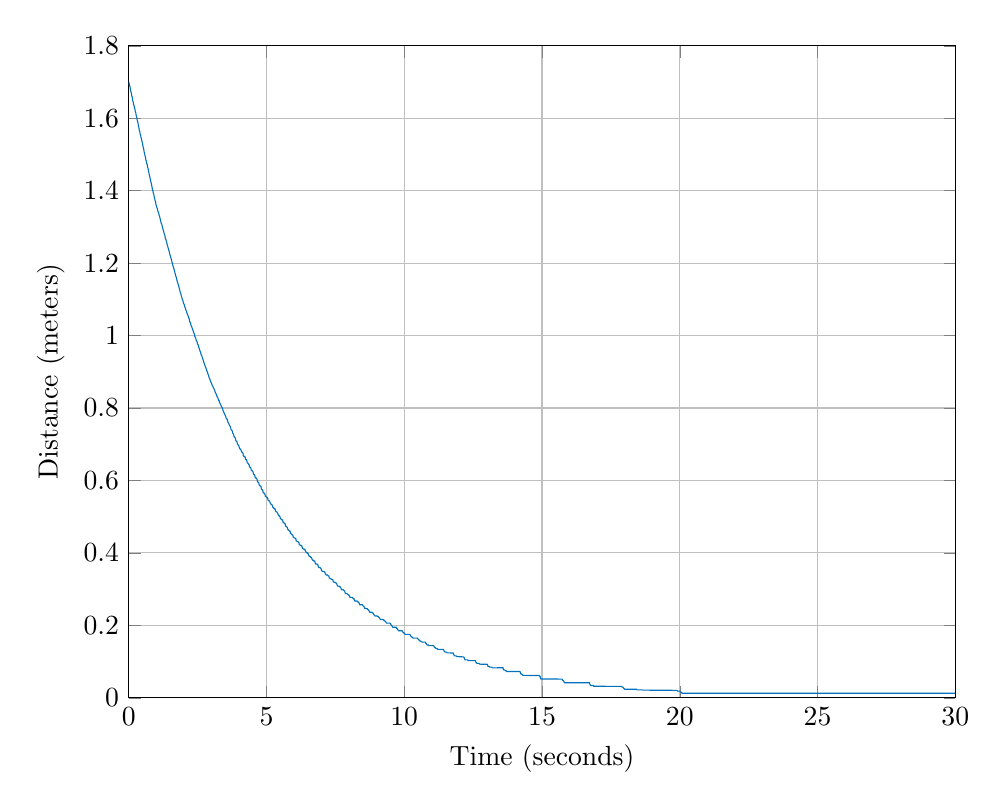
\begin{tikzpicture}

\begin{axis}[%
width=4.133in,
height=3.26in,
at={(0.693in,0.44in)},
scale only axis,
xmin=0,
xmax=30,
xmajorgrids,
xlabel={Time (seconds)},
ymin=0,
ymax=1.8,
ymajorgrids,
ylabel={Distance (meters)},
axis background/.style={fill=white}
]
\addplot [color=mycolor1,solid,forget plot]
  table[row sep=crcr]{%
0	1.70081782542565\\
0.0159694540010001	1.69660589675282\\
0.0318882950010002	1.68882066814531\\
0.0478676570009999	1.68686480946564\\
0.0638765520009995	1.67907958085813\\
0.0798293930019997	1.67321923967272\\
0.0957584119999986	1.66933849357096\\
0.111828809999999	1.66153646812231\\
0.127886796001	1.65862802885522\\
0.143841172	1.64888694156804\\
0.159894290999999	1.64564439032378\\
0.176143369000999	1.63785916171627\\
0.192044619000999	1.6359033030366\\
0.207866816	1.62811807442909\\
0.223849721000999	1.62616221574943\\
0.239858059	1.61837698714192\\
0.255851858999999	1.61545175103369\\
0.27194802	1.60766652242618\\
0.287933	1.60442397118191\\
0.303775710999999	1.5966387425744\\
0.321981479000999	1.59077840138899\\
0.337109563000999	1.58689765528722\\
0.352127729000999	1.57909562983858\\
0.367763166999999	1.57471077137904\\
0.383889255998999	1.56644610328431\\
0.399866684	1.56449024460465\\
0.415800408	1.55626430207136\\
0.431799473001	1.55346246475287\\
0.447792798000999	1.54567723614536\\
0.463857779999999	1.5437213774657\\
0.479858730999999	1.53593614885818\\
0.495828665999999	1.53301091274995\\
0.511860968999999	1.52522568414244\\
0.527849185999999	1.51936534295703\\
0.543860015000999	1.5150438829295\\
0.559898857000999	1.50681375062282\\
0.575870265999999	1.50250095832383\\
0.591837580001	1.49665479155484\\
0.608510514	1.4922699330953\\
0.623894999001	1.48400526500057\\
0.639778625	1.48204940632091\\
0.655995610001	1.4742641777134\\
0.672002625	1.47186760510797\\
0.687832739	1.46408237650046\\
0.704000829	1.46128053918196\\
0.719975892000999	1.4530053726331\\
0.735904739001	1.44861643055851\\
0.752055384	1.44278484585871\\
0.768001442001	1.43692450467329\\
0.784087886	1.43108789989187\\
0.799996302999999	1.42524173312289\\
0.816118343000999	1.42090609867893\\
0.831808307001	1.41463182505191\\
0.847723279999999	1.40982909481157\\
0.863843106999999	1.40156442671684\\
0.879908447000999	1.39960856803718\\
0.895900241000999	1.39182333942967\\
0.911791065001	1.38986748075001\\
0.927809371001	1.38208225214249\\
0.943830726	1.37773203562936\\
0.961128107000999	1.3714105129882\\
0.976439657001	1.36902654745051\\
0.992024755000999	1.36034400757497\\
1.007997327	1.35838814889531\\
1.023950481	1.35254198212632\\
1.040417994	1.3506029202878\\
1.056101545001	1.34474257910239\\
1.071991971001	1.34086183300063\\
1.087883719001	1.33890597432096\\
1.103738822001	1.33261909362621\\
1.121789892001	1.32823423516667\\
1.136671895	1.3238503131737\\
1.152188156001	1.31954146021391\\
1.167995545001	1.31326324724769\\
1.183995688	1.30938250114593\\
1.200010876	1.30742664246627\\
1.216136485	1.30158047569728\\
1.232021814	1.2976855551791\\
1.248096923001	1.29183938841011\\
1.264024122	1.28896967470446\\
1.282604071001	1.28310933351905\\
1.298064838001	1.27874914793007\\
1.313674142	1.27636518239238\\
1.329197981	1.26857995378487\\
1.344857848001	1.2662062233244\\
1.360162801002	1.26230174081865\\
1.375976859001	1.25842099471689\\
1.392090190001	1.25256065353148\\
1.408010759	1.24818996948837\\
1.423828876001	1.244280466901\\
1.440000939001	1.23946779062673\\
1.455996533	1.23557287010854\\
1.471952372	1.23166838760279\\
1.487986734001	1.22540367596334\\
1.503992186	1.22149919345759\\
1.520072341001	1.21720057557502\\
1.536057291	1.21329107298766\\
1.551997861001	1.20939855012638\\
1.568098783	1.20306004775913\\
1.584070708001	1.20110920916109\\
1.599978640001	1.19435245096667\\
1.615990019001	1.19044796846092\\
1.631877809	1.18656722235916\\
1.647998711	1.18222961291377\\
1.664002232001	1.17833709005249\\
1.679982358	1.1724885256266\\
1.695867525	1.16817813098451\\
1.711998397001	1.16379327252497\\
1.727984837	1.15988879001922\\
1.743913597999	1.15552860443024\\
1.759880948	1.14922754931906\\
1.775863833001	1.14728586505582\\
1.791842319	1.14143730062993\\
1.808000155	1.13948646203188\\
1.824027055	1.13322175039243\\
1.840002484001	1.12931726788668\\
1.855905959	1.12494658384357\\
1.871967933	1.11866837087735\\
1.888013665	1.11672668661412\\
1.903988782001	1.11039868270101\\
1.919865690001	1.10800713017719\\
1.935809962	1.10217052539577\\
1.953735545001	1.09826604289002\\
1.968792439999	1.09632435862678\\
1.983878123001	1.09047565643797\\
2.000099749001	1.08809671098189\\
2.015894233	1.0856654272149\\
2.031917720001	1.0798168964031\\
2.047919548001	1.07786605780506\\
2.064109968001	1.07356726902002\\
2.079806403	1.06917836457862\\
2.095816527	1.06722752598058\\
2.111953535	1.06334652361372\\
2.12792502	1.05899626339024\\
2.144020371001	1.05704542479219\\
2.160000594	1.05316433712179\\
2.17600104	1.04925483453442\\
2.191936437001	1.04730387100065\\
2.207879342	1.04055048694375\\
2.223997719001	1.036646004438\\
2.239935156001	1.03664613690712\\
2.255968411001	1.03032958063997\\
2.271989212	1.02600722635341\\
2.287998688	1.02406559358512\\
2.30400662	1.02017007594211\\
2.319995208001	1.01626559343636\\
2.336254670001	1.01388316588628\\
2.35334187	1.00998756317605\\
2.368838891	1.00608308067029\\
2.384244930001	1.00365439484119\\
2.400011289001	0.997805063215115\\
2.415882157001	0.99542611775904\\
2.432003966001	0.993484581348677\\
2.448544359001	0.98715572528634\\
2.464012819	0.985204886688293\\
2.479870780001	0.983263202425058\\
2.495902824001	0.976995896545404\\
2.512001921001	0.975045057947357\\
2.528066186	0.973103373684121\\
2.54401791	0.96681306046018\\
2.559891057001	0.964862221862133\\
2.575978138001	0.960494578182187\\
2.591845722001	0.956585236186437\\
2.607748099	0.95463439758839\\
2.623899212	0.948368579307143\\
2.640006265001	0.945935576445662\\
2.655987495	0.943984737847614\\
2.671922286001	0.938146941711738\\
2.687814431	0.936193298397502\\
2.703767381001	0.931882903755414\\
2.720188110001	0.927986707229218\\
2.736001732001	0.923641431569399\\
2.751909841001	0.92121522615025\\
2.768028476	0.917318945029605\\
2.784062116	0.913414642266995\\
2.799997178001	0.91147295800376\\
2.816017714	0.907576592347775\\
2.831859299	0.903192670354805\\
2.847803170001	0.900822979406111\\
2.863972513	0.896926529273897\\
2.879974552001	0.893022046768146\\
2.895897190001	0.891080383225129\\
2.912016365	0.885230204768097\\
2.928006837	0.882861494389245\\
2.943910818	0.879995871218805\\
2.961380697001	0.876099252311478\\
2.976473772001	0.872194769805727\\
2.991892168001	0.870253121531936\\
3.007861388	0.868312277005391\\
3.023851119001	0.863923673825942\\
3.039826777	0.861973136245442\\
3.056046323	0.860031284744551\\
3.072006477	0.855706390440559\\
3.087764708001	0.853752789389364\\
3.103751797	0.851802051673458\\
3.119862329001	0.849860116642468\\
3.135873738	0.844009601108165\\
3.151858191	0.842058749206424\\
3.167858546	0.839634919360831\\
3.183970187	0.835737963612725\\
3.200006986001	0.832925902681661\\
3.216128766001	0.830975064083614\\
3.231879720001	0.829032962169889\\
3.247856828001	0.825135934488097\\
3.263973536001	0.820754046084643\\
3.280157689001	0.820754046084643\\
3.2960005	0.816870790477519\\
3.312123213001	0.812961287890154\\
3.328027134	0.811010449292107\\
3.343725645	0.808640196485731\\
3.361893023	0.804742904842913\\
3.376973961001	0.802789260935209\\
3.392043457	0.80083841656616\\
3.407818706	0.798415920031513\\
3.423910384	0.792564900655156\\
3.439965633001	0.790614316970719\\
3.45601125	0.787813191316613\\
3.472017779	0.783915732081266\\
3.48789757	0.781962088173562\\
3.503951406001	0.779535616326422\\
3.519985287001	0.777593015184412\\
3.535775659001	0.771741828333811\\
3.552124084	0.769791251157529\\
3.567856432001	0.769791251157529\\
3.584016829	0.767848567017903\\
3.599792720001	0.761569296109768\\
3.615839344	0.759618457511721\\
3.632000571001	0.757675690433656\\
3.647846792	0.753299509207746\\
3.663878683	0.751345865300042\\
3.679958727001	0.749395026701995\\
3.695846331001	0.747452396367645\\
3.711862818	0.741160161352571\\
3.727869106	0.739209322754524\\
3.743818180001	0.73831730720412\\
3.760096399001	0.736374568092309\\
3.776002205	0.730522963591219\\
3.791975233	0.728572124993172\\
3.808011343	0.726629359827046\\
3.823999491001	0.720777671973328\\
3.839964145	0.720777671973328\\
3.855777674	0.71882701257033\\
3.871858458001	0.716455724829794\\
3.887849717	0.710126886767452\\
3.903858751	0.708176412719416\\
3.919799939001	0.708176412719416\\
3.935986685001	0.704277290573925\\
3.953715936	0.700381506031238\\
3.968860583001	0.697989953507419\\
3.984162801002	0.697517294684031\\
3.999801146001	0.695574429000084\\
4.0158895	0.6897224083275\\
4.031844979001	0.687353697948648\\
4.047897556	0.687353868284813\\
4.063859830001	0.685410596837576\\
4.0798626	0.683467995695566\\
4.095793683	0.679558586726525\\
4.114007978	0.677607911475033\\
4.129287465001	0.677607911475033\\
4.144626396	0.675664318267898\\
4.159918868001	0.669337203242811\\
4.175893925	0.666958257786736\\
4.191865109001	0.666958257786736\\
4.207860157001	0.665014956361429\\
4.223855460001	0.665014956361429\\
4.239856176002	0.659162603816739\\
4.255864178	0.657212069337662\\
4.271850160001	0.657212069337662\\
4.287817329001	0.654356892022988\\
4.303791447	0.648504948106912\\
4.319848203001	0.648504948106912\\
4.335875875	0.646554109508865\\
4.351765119	0.644610609967715\\
4.367889995	0.64419273818691\\
4.383856247001	0.638340137359549\\
4.399823647001	0.636389438985245\\
4.416015862001	0.636389651699989\\
4.431861832	0.634445565657103\\
4.447861851001	0.628592882187229\\
4.463926897	0.628120085796484\\
4.479858045001	0.626169247198437\\
4.496011853	0.626169247198437\\
4.51200886	0.623797444565216\\
4.527914738	0.617944595987896\\
4.544011274001	0.615993757389849\\
4.560003209	0.615994160496846\\
4.575877569001	0.61358124118014\\
4.591748465001	0.607728310137891\\
4.609904834002	0.60772890187321\\
4.625266903	0.605337349349391\\
4.640741437001	0.605337349349391\\
4.656413512001	0.603393459537962\\
4.672071667	0.597540363743462\\
4.688013149001	0.595589525145415\\
4.704034682001	0.595171843207891\\
4.719912878	0.593227531558115\\
4.736150858	0.587374353476295\\
4.751936988	0.586903505178412\\
4.767884844	0.584952856941833\\
4.783908802001	0.584952856941833\\
4.799876097001	0.583008198618462\\
4.815924686	0.577155432497912\\
4.831841556	0.574776487041837\\
4.847744050001	0.574776487041837\\
4.863884602	0.572832173865925\\
4.880114166001	0.566512197977933\\
4.895993843001	0.566512197977933\\
4.911960762001	0.564562057429661\\
4.928007231001	0.564562057429661\\
4.944009926002	0.562176440805968\\
4.959826789	0.556323169551408\\
4.975863417001	0.556323169551408\\
4.992000873001	0.554372330953361\\
5.007971996	0.554372573430225\\
5.023981687001	0.552427670732304\\
5.040161729001	0.552427670732304\\
5.055938278001	0.546574167866489\\
5.071956257001	0.544205457487637\\
5.088220264	0.5437365304895\\
5.103892992	0.5437365304895\\
5.119981466001	0.541792141982443\\
5.135996028	0.537894166413416\\
5.15193295	0.535938307733755\\
5.168000948	0.533987908738119\\
5.18400461	0.533987908738119\\
5.199880943	0.532043006040199\\
5.215853741001	0.531615346009703\\
5.231881367	0.525761348311525\\
5.24787841	0.525295136454511\\
5.263997759	0.523344670273207\\
5.280206616001	0.523344670273207\\
5.296572419	0.521399767575286\\
5.312028435001	0.521400147276359\\
5.327975795001	0.515545986365622\\
5.344060890001	0.515105272439849\\
5.359915888	0.513154739309768\\
5.375772964001	0.513154739309768\\
5.39189065	0.511209836611848\\
5.407884746001	0.509256505515655\\
5.423879391	0.505355825537015\\
5.439913648	0.503404986938968\\
5.455996645	0.503404986938968\\
5.471977305001	0.500994111140139\\
5.487869911	0.500576239359335\\
5.503997324001	0.494721834074048\\
5.520000760001	0.494722338349887\\
5.535955648	0.49277149975184\\
5.552002662	0.49277149975184\\
5.568048801002	0.490827108805961\\
5.58400004	0.490827108805961\\
5.599750076001	0.48497254090053\\
5.618062364001	0.484972978907561\\
5.633827361001	0.482127821594471\\
5.649129208001	0.482127821594471\\
5.664260300001	0.480183364439006\\
5.679852359001	0.480183364439006\\
5.695965074001	0.47432863415043\\
5.712014385001	0.472378167527558\\
5.727915283	0.472378167527558\\
5.744020296	0.471937453601786\\
5.759883926002	0.469992550903865\\
5.775998304	0.464138038038995\\
5.792006948	0.464138038038995\\
5.807872076001	0.462187199440948\\
5.823770437	0.462187505621246\\
5.841974467	0.45977876756056\\
5.857190278	0.45977876756056\\
5.871998228001	0.453924366606746\\
5.887992013001	0.453924366606746\\
5.903932317001	0.451973528008699\\
5.919986965001	0.451556236420221\\
5.936077328001	0.4496113337223\\
5.953982919	0.4496113337223\\
5.969192828001	0.44375619851287\\
5.984709469	0.44375619851287\\
5.999959177001	0.441805359914822\\
6.015803117	0.441339148057808\\
6.031876157001	0.441339148057808\\
6.047866945	0.439394245359887\\
6.063821484001	0.439394245359887\\
6.079875703001	0.433111003292429\\
6.095787981001	0.433111003292429\\
6.111824279001	0.431160164694381\\
6.127990720001	0.431160164694381\\
6.143943447	0.431160164694381\\
6.159873066	0.429215261996461\\
6.175919849	0.429215261996461\\
6.19188774	0.422919412861258\\
6.207894863	0.422919412861258\\
6.223888216001	0.420968574263211\\
6.23979112	0.420968574263211\\
6.257935026001	0.420968574263211\\
6.273032035001	0.41902367156529\\
6.288366658	0.41902367156529\\
6.303932743001	0.412705380118768\\
6.319977589	0.412705380118768\\
6.336104430001	0.410754541520721\\
6.351773812001	0.410754541520721\\
6.367831019001	0.410754541520721\\
6.383973666001	0.408809638822801\\
6.400002892001	0.408809638822801\\
6.415959868001	0.404910362293032\\
6.431856122	0.40295450361337\\
6.447845472001	0.400585793234518\\
6.463804643002	0.400585793234518\\
6.479853794	0.400585793234518\\
6.495915801	0.398174678679583\\
6.511892534001	0.398174678679583\\
6.527997933	0.394275402149814\\
6.543801605001	0.392319543470153\\
6.559796773001	0.390368704872105\\
6.5759162	0.390368704872105\\
6.591979767	0.389940598014077\\
6.607971548001	0.387995695316157\\
6.624039766	0.387995695316157\\
6.640008590001	0.386042051408453\\
6.656018411	0.382140560106726\\
6.672016024001	0.380189721508679\\
6.68795965	0.379749007582907\\
6.703910555001	0.379749007582907\\
6.719854092	0.377804104884986\\
6.735810305001	0.377804104884986\\
6.751784583001	0.377804104884986\\
6.767881734001	0.371948969675556\\
6.783847591001	0.369534974840417\\
6.799851885001	0.369534974840417\\
6.815858068001	0.369534974840417\\
6.831848505001	0.369534974840417\\
6.847735393002	0.367590072142496\\
6.865961495001	0.367590072142496\\
6.881432701001	0.361734936933066\\
6.896927412001	0.359784098335019\\
6.912305057001	0.359784098335019\\
6.928204686	0.359784098335019\\
6.944015121001	0.359784244353701\\
6.961768003001	0.35783934165578\\
6.977286168	0.35695491666259\\
6.992369866001	0.353055453089272\\
7.007864050001	0.351099740393534\\
7.023878667	0.349148901795486\\
7.039984616001	0.349148796126405\\
7.056008674	0.349148796126405\\
7.071943774001	0.349148796126405\\
7.088002959	0.349148796126405\\
7.103736639	0.347203796112126\\
7.119974939001	0.347203796112126\\
7.136014087001	0.341348953108839\\
7.151959142001	0.341348937345672\\
7.167844505001	0.338969991889597\\
7.183989243001	0.338969991889597\\
7.199888128001	0.338969984538724\\
7.215862278	0.338969984538724\\
7.231880594	0.337025081840804\\
7.247848936	0.336584368976455\\
7.263789964	0.336584368976455\\
7.279854211	0.330729745753269\\
7.295857823	0.330729828606151\\
7.311976275	0.328778990008104\\
7.328029225001	0.328315833771012\\
7.343993202001	0.32831592509575\\
7.359822577001	0.32831592509575\\
7.375907272	0.32637102239783\\
7.391866144001	0.32637102239783\\
7.408044163001	0.326371122194421\\
7.424005856	0.320516719287405\\
7.440030210001	0.320516719287405\\
7.456122597999	0.31856606251564\\
7.472013515001	0.31856606251564\\
7.488020871001	0.31856606251564\\
7.503924189001	0.318566252873323\\
7.519919810001	0.316621350175402\\
7.535845886001	0.316621350175402\\
7.551858930001	0.314666643539413\\
7.567845939999	0.310301155152629\\
7.583888009	0.308350316554582\\
7.599911205	0.308350597711546\\
7.615891936	0.308350597711546\\
7.63210608	0.307927948118635\\
7.647949425001	0.307927896690459\\
7.663996987001	0.305982993992538\\
7.679972486001	0.305982993992538\\
7.696008689001	0.304028267031228\\
7.711996321001	0.300128990501459\\
7.728059975001	0.298178151903412\\
7.743928292	0.298178151903412\\
7.760091499001	0.298178191597983\\
7.776107522001	0.298178191597983\\
7.792053229001	0.298178191597983\\
7.808130084	0.296233337257983\\
7.824202266	0.295805230399955\\
7.840133195	0.293850694152818\\
7.855752339001	0.289510834752758\\
7.871983758001	0.28755999615471\\
7.887775662	0.28755999615471\\
7.903987596	0.287560135933074\\
7.919982558	0.287560135933074\\
7.935932122	0.287096979695983\\
7.951880379	0.285152379468149\\
7.968029977001	0.285153032821687\\
7.983995293001	0.28319871885579\\
7.999873571001	0.283198950292721\\
8.015923343	0.279300337040956\\
8.031882722001	0.277349498442909\\
8.047813257	0.277349738662239\\
8.063852334	0.277350500314979\\
8.079913326001	0.277350500314979\\
8.095938065001	0.277350500314979\\
8.11178358	0.277350929617033\\
8.127979052001	0.275406300836564\\
8.143977904001	0.275406300836564\\
8.1599744	0.273452649837989\\
8.175954328001	0.273453257549888\\
8.192015546001	0.269553577580948\\
8.208010358001	0.267139021907085\\
8.223865609	0.267139557900118\\
8.239883278	0.267139557900118\\
8.25584028	0.267140372948655\\
8.27197751	0.267140917792092\\
8.288412248001	0.267140917792092\\
8.304001652001	0.265195805661753\\
8.319944536001	0.265196752470437\\
8.336003705	0.263242959244274\\
8.351779197001	0.262815635540459\\
8.367727617	0.260870242363735\\
8.383984457001	0.256965759857983\\
8.399992967	0.256965759857983\\
8.415812083001	0.256966280884559\\
8.431915846001	0.256966772006241\\
8.44811436	0.256966772006241\\
8.464048484001	0.256967310856964\\
8.479983796001	0.256967810888273\\
8.495937310001	0.25502201671272\\
8.511972419001	0.25306899834854\\
8.528065894001	0.25306950728946\\
8.544046625	0.251122908903198\\
8.560002995	0.247218995135369\\
8.576011168001	0.247219432890907\\
8.592007989001	0.247219432890907\\
8.607794052001	0.24679191271368\\
8.623926568	0.246351645512324\\
8.639961872	0.246351645512324\\
8.656101613	0.246351875162964\\
8.671882595001	0.243948528256623\\
8.687855839	0.243948528256623\\
8.704042826001	0.241995572357011\\
8.720027245	0.240049761894432\\
8.736062063	0.238096117986728\\
8.752129234001	0.236145279388681\\
8.768989346001	0.236146648193631\\
8.784419705	0.236146648193631\\
8.800021111001	0.236146648193631\\
8.816028332	0.236147301478628\\
8.831998363	0.236148044102232\\
8.847965608	0.234201686356678\\
8.863936822001	0.23420227743038\\
8.879968056	0.232250060066937\\
8.896000960001	0.230302902261191\\
8.911959159001	0.228349942832025\\
8.927869045001	0.226399785261811\\
8.943854726	0.226399785261811\\
8.961113090001	0.225940365222474\\
8.976079854001	0.225940365222474\\
8.991879459	0.225940363945597\\
9.008106522001	0.225940363945597\\
9.024076152001	0.225940363945597\\
9.039871969001	0.223993853555945\\
9.055871763001	0.223993853555945\\
9.072000979001	0.222040959810853\\
9.087978452001	0.222040976772396\\
9.103879567001	0.220093739286816\\
9.120004955	0.218140095379112\\
9.135866155001	0.216189591013562\\
9.151997411001	0.216189591013562\\
9.167872838001	0.216189591013562\\
9.183855112001	0.216189703400006\\
9.199852871001	0.216189703400006\\
9.215834248001	0.215758187443893\\
9.231828539001	0.215758187443893\\
9.247825505999	0.215758309008958\\
9.263814235	0.213811790776971\\
9.279848972001	0.213811790776971\\
9.295860131001	0.211859027775562\\
9.31183108	0.211859027775562\\
9.327997851	0.209911790289982\\
9.343974533	0.207958286304574\\
9.35978622	0.206008064960682\\
9.375874026	0.206008064960682\\
9.392014445	0.206008291485714\\
9.408040734001	0.206008291485714\\
9.423919187001	0.206008291485714\\
9.439831803001	0.206008527248755\\
9.455991905	0.206008527248755\\
9.472023130001	0.206008527248755\\
9.487974574001	0.206008772249799\\
9.504071444001	0.204062254017813\\
9.519993851	0.201681253414693\\
9.535979497001	0.19928955747661\\
9.552070488	0.198833109495035\\
9.567891937001	0.19687946558733\\
9.58386491	0.194929554296363\\
9.599760848001	0.194929555118175\\
9.615877495	0.194929555118175\\
9.631895822001	0.194929555118175\\
9.648131179	0.194929565250921\\
9.664104951001	0.194929565250921\\
9.680019963001	0.194929565250921\\
9.695887771	0.194929584694601\\
9.711871261001	0.194929584694601\\
9.727793479001	0.191030172717522\\
9.743805853	0.191030201472136\\
9.759848071001	0.189082963986556\\
9.775891438001	0.187129320078852\\
9.791840762001	0.185179835756015\\
9.807944975001	0.185179835756015\\
9.823916602001	0.185179835756015\\
9.839908965001	0.185179961091176\\
9.855862528001	0.185179961091176\\
9.871878964	0.185179961091176\\
9.888000675001	0.185180095796651\\
9.903982832001	0.185180095796651\\
9.919822709002	0.185180095796651\\
9.936025392	0.182767782012221\\
9.953887003001	0.180821407856019\\
9.969278449001	0.180821407856019\\
9.984745074001	0.178874170370439\\
10.00019827	0.178874170370439\\
10.016219101	0.176920526462735\\
10.031980094	0.174971238128553\\
10.047881965001	0.174971238128553\\
10.063866920001	0.174971238128553\\
10.079859978001	0.174971238128553\\
10.095926483	0.174971238128553\\
10.111912972001	0.174971238128553\\
10.127851591001	0.174971238128553\\
10.143813294001	0.174971238128553\\
10.159868603001	0.174971238128553\\
10.175986284001	0.174971238128553\\
10.191939165	0.174971238128553\\
10.208009068001	0.174971238128553\\
10.224008927001	0.171071826151474\\
10.240032097999	0.171071826151474\\
10.255999123001	0.169124588665895\\
10.272034271	0.168693072709782\\
10.288020534001	0.166739428802078\\
10.304004382	0.166739428802078\\
10.319990404001	0.164790140467896\\
10.335917867	0.164790140467896\\
10.351760952	0.164790140467896\\
10.370194304	0.164790140467896\\
10.385690491001	0.164790140467896\\
10.401205191	0.164790140467896\\
10.41661386	0.164790140467896\\
10.431854941	0.164790140467896\\
10.447856383001	0.164790140467896\\
10.463908189001	0.164790140467896\\
10.480000116001	0.164790140467896\\
10.496004439999	0.162837246722804\\
10.511886587	0.160890728490817\\
10.527800082	0.160890728490817\\
10.543839494001	0.158943491005237\\
10.559806553001	0.156989847097533\\
10.575772662	0.156989847097533\\
10.591810854001	0.156989847097533\\
10.607699495	0.155040558763351\\
10.623859253001	0.154584196873232\\
10.640121188001	0.154136675934926\\
10.655977509	0.154136675934926\\
10.671882799	0.153708569076898\\
10.687784198	0.153708569076898\\
10.70385336	0.153708569076898\\
10.719861047	0.153708569076898\\
10.735982426002	0.153708569076898\\
10.752111733	0.153708569076898\\
10.768063528	0.153708569076898\\
10.784025014	0.14980915709982\\
10.800012039	0.14980915709982\\
10.815895222999	0.14786191961424\\
10.832004064001	0.145908275706536\\
10.847837703001	0.145908275706536\\
10.863762269001	0.145908275706536\\
10.879901053001	0.145908275706536\\
10.895978662	0.143958987372354\\
10.911990757001	0.143958987372354\\
10.927868180001	0.143958987372354\\
10.943849537	0.143958987372354\\
10.9598092	0.143959342625628\\
10.978044492	0.143959993852696\\
10.993141611001	0.143959993852696\\
11.008203345001	0.143959993852696\\
11.02397003	0.143961029139809\\
11.039859694	0.143961029139809\\
11.056027263001	0.143961029139809\\
11.072006309001	0.143962093233663\\
11.087968984	0.140062907465499\\
11.103846997	0.140062907465499\\
11.119867538001	0.138116573117771\\
11.135970645001	0.138116520276272\\
11.152038305001	0.135703755680266\\
11.167869549	0.135704224894894\\
11.183897406001	0.135704948572212\\
11.199852433	0.135704948572212\\
11.215978428001	0.13375613910709\\
11.232004681001	0.133756882114922\\
11.248011751	0.133756882114922\\
11.264223324	0.133757370638399\\
11.280320318001	0.133758132976722\\
11.295989633	0.133758132976722\\
11.312168236001	0.133758631154602\\
11.328021027	0.133759412823393\\
11.343901695	0.133759412823393\\
11.359818206	0.133759412823393\\
11.375714615001	0.133760721654895\\
11.391991887001	0.133760721654895\\
11.407988724	0.133760721654895\\
11.423850029001	0.13376205947119\\
11.439801002	0.129863403605577\\
11.455850804	0.127915372584456\\
11.471849014	0.127915975663697\\
11.488306594001	0.125963917894919\\
11.5040205	0.125963917894919\\
11.519858722999	0.125964530687963\\
11.536025139001	0.125965386113475\\
11.552076148001	0.124016097779293\\
11.567988053	0.124016720286121\\
11.583898343	0.124017595160806\\
11.599761806001	0.124017595160806\\
11.618152858001	0.1240182273814\\
11.633702861001	0.12401912170523\\
11.64903883	0.12401912170523\\
11.664473141	0.12401912170523\\
11.679952448001	0.123584050277158\\
11.695972144001	0.123584050277158\\
11.711975551002	0.123584050277158\\
11.727920185	0.123585294507997\\
11.743914509001	0.123585294507997\\
11.759988316	0.123585294507997\\
11.775765118001	0.123586344449667\\
11.791688213001	0.119691466717542\\
11.809922345001	0.117739861900275\\
11.825132179	0.115788563942002\\
11.840278374001	0.115788872894185\\
11.855731909	0.115788872894185\\
11.871869125	0.115789289497894\\
11.8881146	0.115790278333932\\
11.904005517001	0.113840989999749\\
11.919997548001	0.113841416389891\\
11.936032416001	0.113842424793732\\
11.951897334002	0.113842830790341\\
11.967898961001	0.113842830790341\\
11.983864117	0.113843520450134\\
11.999855992	0.113394298607473\\
12.015856052001	0.113394714385786\\
12.031854833001	0.113395753980339\\
12.047767614001	0.113395753980339\\
12.06393782	0.113396179540344\\
12.079890761	0.113397228929765\\
12.096041843	0.11294970799146\\
12.11191199	0.112950143333142\\
12.127900305	0.112950143333142\\
12.143855736001	0.1129512025174\\
12.159904873001	0.112951647640748\\
12.175953924001	0.110567591899871\\
12.191850388	0.106670288696744\\
12.207804507001	0.104718526110348\\
12.223857853	0.104718526110348\\
12.239873893	0.104719526747354\\
12.255804513001	0.104719911635533\\
12.271882992	0.104719911635533\\
12.287889340001	0.104720922126655\\
12.304014357001	0.104720922126655\\
12.319972557001	0.102772028521587\\
12.336040751001	0.102773048866796\\
12.351946145	0.102773048866796\\
12.367927983	0.102773453436832\\
12.384006744	0.102774483636096\\
12.399956556	0.102774483636096\\
12.415911989001	0.102774898047043\\
12.432006647001	0.102775938100331\\
12.448116886001	0.102775938100331\\
12.463871394001	0.102776362352176\\
12.479862618001	0.102776362352176\\
12.49595001	0.102777412259456\\
12.511967063001	0.102777846352186\\
12.528033015001	0.102777846352186\\
12.543790333	0.102778906113427\\
12.560001378	0.102779350047028\\
12.576006939001	0.102779350047028\\
12.592158342	0.10083058603296\\
12.607777668	0.0969316548456216\\
12.624004190001	0.0969320292368536\\
12.639837188	0.0949808934105594\\
12.655819171001	0.0949808934105594\\
12.671823888	0.0949812777019641\\
12.687753115	0.0949822894225572\\
12.703743720001	0.0949822894225572\\
12.71973295	0.0949826836141225\\
12.735737011	0.0930344169137634\\
12.751866009	0.0930344169137634\\
12.76788212	0.0930348210054781\\
12.7840074	0.0925811784157609\\
12.799983347001	0.0925822099627818\\
12.815895186	0.0925829639294768\\
12.831852253001	0.0925829639294768\\
12.847885686001	0.0925840053896645\\
12.864230788001	0.0925847692702919\\
12.880054618001	0.0925847692702919\\
12.895771613	0.0925858206436145\\
12.911885618001	0.0925865944381512\\
12.927876244001	0.0925865944381512\\
12.943874411001	0.0925876557245771\\
12.961217353	0.0925876557245771\\
12.976316993001	0.0925884394329994\\
12.991836163001	0.0925884394329994\\
13.007977505001	0.0925884394329994\\
13.023887656001	0.0906388570413628\\
13.040007793001	0.0867392135409968\\
13.056009876001	0.0867392135409968\\
13.072052893	0.0867399382279326\\
13.088175309	0.0867399382279326\\
13.104558904	0.0847878005943059\\
13.119827645	0.0847885352544049\\
13.136044119001	0.0847885352544049\\
13.151940559	0.0847885352544049\\
13.167903213001	0.0847892798876451\\
13.183993417001	0.0847892798876451\\
13.200132721001	0.0828399915534632\\
13.216019143002	0.0828407461598213\\
13.231977427001	0.0828407461598213\\
13.248086624001	0.0828407461598213\\
13.264002327	0.0828407461598213\\
13.280311245001	0.0828415107392746\\
13.296000656001	0.0828415107392746\\
13.311964234001	0.0828415107392746\\
13.327993303001	0.0828422852917998\\
13.344013347001	0.0828422852917998\\
13.359728674	0.0828422852917998\\
13.377883927001	0.0828430698173732\\
13.392957954001	0.0828430698173732\\
13.408048753001	0.0828430698173732\\
13.42410304	0.082843864315971\\
13.440018252	0.082843864315971\\
13.4560002	0.082843864315971\\
13.471899461001	0.082844668787569\\
13.487948045001	0.082844668787569\\
13.503864039	0.082844668787569\\
13.519803004001	0.0828454832321426\\
13.536005597001	0.0828454832321426\\
13.552066305001	0.0828454832321426\\
13.568004939001	0.0828463076496675\\
13.584007895	0.0828463076496675\\
13.599835951	0.0769954240589836\\
13.615950954001	0.0769954240589836\\
13.631909479001	0.07699618025323\\
13.647794673001	0.07699618025323\\
13.663833295001	0.0750440426196031\\
13.679856596	0.0746064786476408\\
13.695911985	0.0746064786476408\\
13.711826235	0.072657190313459\\
13.727811329	0.0726579665722358\\
13.743813842001	0.0726579665722358\\
13.759800265001	0.0726579665722358\\
13.777982546001	0.0726587528632416\\
13.793340385001	0.0726587528632416\\
13.808944668001	0.0726587528632416\\
13.824406989001	0.0726595491864535\\
13.839999786001	0.0726595491864535\\
13.855767228	0.0726595491864535\\
13.871938951001	0.072660355541847\\
13.888144706001	0.072660355541847\\
13.903860076001	0.072660355541847\\
13.920018559	0.072660355541847\\
13.935897262001	0.0726611719293973\\
13.953966564001	0.0726611719293973\\
13.968983581	0.0726615736644387\\
13.984183869001	0.0726615736644387\\
13.999917484001	0.0726615736644387\\
14.015986164	0.0726615736644387\\
14.031881256001	0.0726619854370081\\
14.048005055	0.0726619854370081\\
14.064019341001	0.0726619854370081\\
14.079881579	0.0726624072470936\\
14.095941288001	0.0726624072470936\\
14.111871618001	0.0726624072470936\\
14.127878213001	0.0726628390946824\\
14.143979587	0.0726628390946824\\
14.160135745	0.0726628390946824\\
14.175988168001	0.0726632809797609\\
14.192007126001	0.0726632809797609\\
14.20804233	0.071773003444302\\
14.223825182001	0.0659224857379215\\
14.239822188	0.0659224857379215\\
14.255948699	0.0659224857379215\\
14.272010103001	0.0639708869536892\\
14.287997137001	0.0639708869536892\\
14.304005165	0.0620215986195074\\
14.319911938	0.0620221475657767\\
14.335990881001	0.0620221475657767\\
14.351851362001	0.0620221475657767\\
14.367852289	0.0620221475657767\\
14.383976385001	0.0620227066089043\\
14.400008391	0.0620227066089043\\
14.415964681	0.0620227066089043\\
14.431993646	0.0620232757488726\\
14.448088074001	0.0620232757488726\\
14.464059366001	0.0620232757488726\\
14.480057723001	0.0620238549856644\\
14.495990735	0.0620238549856644\\
14.512023238	0.0620238549856644\\
14.527984875	0.061589520579536\\
14.544007420001	0.061589520579536\\
14.559926185001	0.061589520579536\\
14.575876566001	0.0615901200099216\\
14.591935310001	0.0615901200099216\\
14.607909262001	0.0615901200099216\\
14.623888641001	0.0615907295370768\\
14.639906203001	0.0615907295370768\\
14.655787535	0.0615907295370768\\
14.671761170001	0.0615907295370768\\
14.687844594001	0.0615913491609827\\
14.703959004	0.0615913491609827\\
14.719985019001	0.0615913491609827\\
14.735871314999	0.061591978881621\\
14.751860811	0.061591978881621\\
14.767807950001	0.061591978881621\\
14.783975373001	0.0615926186989724\\
14.799899113	0.0615926186989724\\
14.815996178001	0.0615926186989724\\
14.832037977001	0.0615932686130172\\
14.847852678001	0.0615932686130172\\
14.863939973001	0.0615932686130172\\
14.879966878001	0.0615939286237355\\
14.895984371001	0.0615939286237355\\
14.91201907	0.0596417909901084\\
14.927973691001	0.0596424610974806\\
14.944052192	0.0537936610064711\\
14.961804220001	0.0518432849925503\\
14.977068507	0.0518440429176819\\
14.992567572	0.0518440429176819\\
15.008002741001	0.0518440429176819\\
15.023863630001	0.0518440429176819\\
15.039855266	0.0518448109988194\\
15.055963595	0.0518448109988194\\
15.072039025	0.0518448109988194\\
15.087869004	0.0518455892359386\\
15.103848532001	0.0518455892359386\\
15.119959711001	0.0518455892359386\\
15.136018104001	0.0518463776290163\\
15.152008766001	0.0518463776290163\\
15.167997014	0.0518463776290163\\
15.183953546	0.0518471761780281\\
15.200059665	0.0518471761780281\\
15.215998013001	0.0518471761780281\\
15.231898588001	0.0518479848829498\\
15.247978943	0.0518479848829498\\
15.264080708001	0.0518479848829498\\
15.280513096	0.0518488037437574\\
15.295994695	0.0518488037437574\\
15.312041350001	0.0518488037437574\\
15.328041405	0.0518488037437574\\
15.344002701001	0.051849632760425\\
15.359762201001	0.051849632760425\\
15.375960153	0.051849632760425\\
15.391997050001	0.0518504719329278\\
15.408011742	0.0518504719329278\\
15.423880785	0.0518504719329278\\
15.439852134	0.0518513212612404\\
15.456127462	0.0518513212612404\\
15.47217233	0.0518513212612404\\
15.488013696001	0.0518521807453363\\
15.50400441	0.0518521807453363\\
15.519979112	0.0518521807453363\\
15.535884546	0.0518530503851902\\
15.551852478001	0.0518530503851902\\
15.567889716001	0.0518530503851902\\
15.584001579001	0.0518539301807748\\
15.599848724	0.0514081104876321\\
15.615941621001	0.0514081104876321\\
15.631813304	0.0514081104876321\\
15.648003217	0.0514090004389209\\
15.663912808	0.0514090004389209\\
15.679911449	0.0514090004389209\\
15.695815934	0.051409900545887\\
15.711794112	0.051409900545887\\
15.727791006001	0.051409900545887\\
15.743853849	0.0494586731748761\\
15.759793651	0.0475100902094887\\
15.775777561	0.0475100902094887\\
15.791849662	0.045561800964673\\
15.807969437001	0.0416617468231617\\
15.823996207001	0.0416617468231617\\
15.839959287001	0.0416627561274767\\
15.855920874001	0.0416627561274767\\
15.871993934	0.0416627561274767\\
15.887972512001	0.04166377564671\\
15.904018626001	0.04166377564671\\
15.919991285	0.04166377564671\\
15.936004965001	0.0416648053808302\\
15.953856455001	0.0416648053808302\\
15.968970735	0.0416648053808302\\
15.984120012001	0.0416667641303503\\
15.999811463001	0.0416667641303503\\
16.015854143002	0.0416667641303503\\
16.031858688001	0.0416687433273122\\
16.047856271	0.0416687433273122\\
16.063826012001	0.0416687433273122\\
16.079838534	0.0416707429716556\\
16.095809988	0.0416707429716556\\
16.111717761	0.0416707429716556\\
16.129884726	0.0416727630633189\\
16.145144315001	0.0416727630633189\\
16.16055173	0.0416727630633189\\
16.175986544001	0.0416737373265077\\
16.192011208001	0.0416748036022418\\
16.208162876001	0.0416748036022418\\
16.224048015	0.0416757880891696\\
16.239851915	0.0416768645883616\\
16.255813015001	0.0416768645883616\\
16.271974621001	0.0416768645883616\\
16.288371905	0.0416789460216154\\
16.303987031001	0.0416789460216154\\
16.320003543001	0.0416789460216154\\
16.335916626001	0.0416810479019398\\
16.351941226001	0.0416810479019398\\
16.367831852001	0.0416810479019398\\
16.383788065001	0.041683170229271\\
16.399795587	0.041683170229271\\
16.415819438	0.041683170229271\\
16.431999064001	0.0416841956108516\\
16.447705063001	0.0416853130035437\\
16.463956152001	0.0416853130035437\\
16.479921340001	0.0416863486087105\\
16.495985787	0.0416874762246937\\
16.511869347001	0.0416874762246937\\
16.527862682001	0.0416885220534147\\
16.543845256001	0.0416896598926542\\
16.559969141	0.0416896598926542\\
16.575906971001	0.0416896598926542\\
16.591902972999	0.0416918640073591\\
16.607812722001	0.0416918640073591\\
16.623878536001	0.0416918640073591\\
16.639991251	0.0416940885687413\\
16.655851253001	0.0416940885687413\\
16.671873748001	0.0416940885687413\\
16.688108242	0.0416963335767326\\
16.704007151	0.0416963335767326\\
16.720109409	0.0416963335767326\\
16.736056718	0.0377981934728844\\
16.751979347001	0.0358472779854599\\
16.767920748001	0.0338956731681934\\
16.784131810001	0.0338966932842535\\
16.800033136001	0.0338978059442594\\
16.815923112001	0.0338978059442594\\
16.8319206	0.0338988363431083\\
16.848102135001	0.03389995928561\\
16.863789490001	0.03389995928561\\
16.879666708001	0.0319517116330348\\
16.895682828001	0.0319528448579975\\
16.911816294	0.0319528448579975\\
16.927757428	0.0319528448579975\\
16.943975692001	0.0319550393297201\\
16.961780048001	0.0319550393297201\\
16.977132145001	0.0319550393297201\\
16.992219702	0.0319561005767475\\
17.00801423	0.0319561005767475\\
17.023976394001	0.0319561005767475\\
17.039866539	0.0319571721064362\\
17.055861285	0.0319571721064362\\
17.071862212001	0.0319571721064362\\
17.087985823	0.0319582539187542\\
17.103824337	0.0319582539187542\\
17.119991166	0.0319582539187542\\
17.135998016	0.0319593460136682\\
17.152045182001	0.0319593460136682\\
17.168007185	0.0319593460136682\\
17.184082439001	0.0319604483911451\\
17.200036305001	0.0319604483911451\\
17.215911741001	0.0319604483911451\\
17.231975214001	0.0319604483911451\\
17.248002520001	0.0319615610511514\\
17.264079904001	0.0319615610511514\\
17.280322427001	0.0319615610511514\\
17.29611875	0.0319626839936531\\
17.311875122	0.0315107414161331\\
17.327970567001	0.0315107414161331\\
17.343818283	0.0315118746410958\\
17.359726566	0.0315118746410958\\
17.377905206001	0.0315118746410958\\
17.393368992	0.0315130181484857\\
17.408637049	0.0315130181484857\\
17.423841734001	0.0315130181484857\\
17.439981289	0.0315141719382668\\
17.456027709	0.0315141719382668\\
17.471980646	0.0315141719382668\\
17.487988438	0.031515336010405\\
17.504054552001	0.031515336010405\\
17.520015191	0.031515336010405\\
17.535965709002	0.0315165103648645\\
17.551995124001	0.0315165103648645\\
17.567856965001	0.0315165103648645\\
17.583864175001	0.0315165103648645\\
17.599964472001	0.0315176950016094\\
17.615728743001	0.0315176950016094\\
17.633852895001	0.0315176950016094\\
17.649163610001	0.0315188899206038\\
17.664543462	0.0315188899206038\\
17.680056236001	0.0315188899206038\\
17.695979270001	0.0315200951218113\\
17.711922886001	0.0315200951218113\\
17.727974091001	0.0315200951218113\\
17.74393249	0.0315213106051946\\
17.759977632	0.0315213106051946\\
17.775970189001	0.0315213106051946\\
17.792165029001	0.0315225363707174\\
17.808070895001	0.0315225363707174\\
17.823900203001	0.0315225363707174\\
17.839848981	0.0315237724183421\\
17.855793231	0.0315237724183421\\
17.873941960001	0.0315237724183421\\
17.889012665	0.0315250187480312\\
17.904434668001	0.0295723512118533\\
17.919892484001	0.0295723512118533\\
17.935898036001	0.0295723512118533\\
17.951833448	0.0276213947274853\\
17.96800015	0.0256731268027315\\
17.984071070001	0.0256731268027315\\
18.000002734001	0.0237212171622263\\
18.016052199001	0.0237212171622263\\
18.032050345001	0.0237212171622263\\
18.048000902001	0.0237212171622263\\
18.063996817001	0.0237212171622263\\
18.080001712	0.0237212171622263\\
18.095985454	0.0237212171622263\\
18.113331317	0.0237212171622263\\
18.129199355	0.0237212171622263\\
18.144652818	0.0237212171622263\\
18.160029415001	0.0237212171622263\\
18.17602786	0.0237212171622263\\
18.191983163001	0.0237212171622263\\
18.208008479001	0.0237212171622263\\
18.223971984001	0.0237212171622263\\
18.240008046001	0.0237212171622263\\
18.255872819001	0.0237212171622263\\
18.271998062	0.0237212171622263\\
18.288011171001	0.0237212171622263\\
18.303961988	0.0237212171622263\\
18.319878568	0.0237212171622263\\
18.335918817001	0.0237212171622263\\
18.351935164	0.0237212171622263\\
18.367962300001	0.0237212171622263\\
18.384059128001	0.0237212171622263\\
18.399863258	0.0237212171622263\\
18.415899590001	0.0237212171622263\\
18.431852422	0.0237212171622263\\
18.447827199001	0.0217719288280445\\
18.463805599	0.0217719288280445\\
18.479805267	0.0217719288280445\\
18.495812894001	0.0217719288280445\\
18.511929757	0.0217719288280445\\
18.527999685	0.0217719288280445\\
18.544013164001	0.0217719288280445\\
18.560075214	0.0217719288280445\\
18.575978033	0.0217719288280445\\
18.592012551002	0.0217719288280445\\
18.607754555001	0.0217719288280445\\
18.623839748001	0.0217719288280445\\
18.639926007001	0.0217719288280445\\
18.655985630001	0.0217719288280445\\
18.671967508	0.0213359830111095\\
18.688034318	0.0213359830111095\\
18.704034719	0.0213359830111095\\
18.719984599	0.0213359830111095\\
18.736128654001	0.0213359830111095\\
18.751965058	0.0213359830111095\\
18.767996242	0.0213359830111095\\
18.783912416001	0.0213359830111095\\
18.799775550001	0.0213359830111095\\
18.815839352001	0.0213359830111095\\
18.831878422	0.0213359830111095\\
18.848115756001	0.0213359830111095\\
18.863726013001	0.0213359830111095\\
18.879897306001	0.0213359830111095\\
18.896090207001	0.0213359830111095\\
18.911955977001	0.0208884620728038\\
18.927995727001	0.0208884620728038\\
18.944009462	0.0208884620728038\\
18.961725567001	0.0208884620728038\\
18.977259065001	0.0208884620728038\\
18.992755965001	0.0208884620728038\\
19.008347885001	0.0208884620728038\\
19.024072465001	0.0208884620728038\\
19.039952397001	0.0208884620728038\\
19.056006648001	0.0208884620728038\\
19.071988015001	0.0208884620728038\\
19.088057637001	0.0208884620728038\\
19.103933689999	0.0208884620728038\\
19.119852371001	0.0208884620728038\\
19.135899882	0.0208884620728038\\
19.151843198001	0.0208884620728038\\
19.168042835001	0.0208884620728038\\
19.184036679001	0.0208884620728038\\
19.199869263	0.0208884620728038\\
19.215856338001	0.0208884620728038\\
19.231850979001	0.0208884620728038\\
19.247834993001	0.0208884620728038\\
19.264000773	0.0208884620728038\\
19.279884638001	0.0208884620728038\\
19.296015865	0.0208884620728038\\
19.312010983	0.0208884620728038\\
19.328025689999	0.0208884620728038\\
19.344093302001	0.0208884620728038\\
19.359960927001	0.0208884620728038\\
19.375929534	0.0208884620728038\\
19.391970817001	0.0208884620728038\\
19.407978603	0.0208884620728038\\
19.423989763	0.0208884620728038\\
19.439866197001	0.0208884620728038\\
19.455855216001	0.0208884620728038\\
19.471984799	0.0208884620728038\\
19.488003545001	0.0208884620728038\\
19.503918797	0.0208884620728038\\
19.519865866001	0.0208884620728038\\
19.535863801002	0.0208884620728038\\
19.551890405	0.0208884620728038\\
19.567851947001	0.0208884620728038\\
19.583863026	0.0208884620728038\\
19.601002812001	0.0208884620728038\\
19.615748700001	0.0208884620728038\\
19.631972063	0.0208884620728038\\
19.648004031001	0.0208884620728038\\
19.664037742	0.0208884620728038\\
19.679867420001	0.0208884620728038\\
19.695865039	0.0208884620728038\\
19.711845538001	0.0204535383330782\\
19.728057954001	0.0204535383330782\\
19.744038453001	0.0204535383330782\\
19.760220520001	0.0204535383330782\\
19.776029712	0.0204535383330782\\
19.792017889	0.0204535383330782\\
19.808082404001	0.0204535383330782\\
19.824062608	0.0204535383330782\\
19.840111929001	0.0204535383330782\\
19.855750574001	0.0204535383330782\\
19.874019082	0.0204535383330782\\
19.889563369001	0.0204535383330782\\
19.905239269001	0.0204535383330782\\
19.920471188001	0.018500795334444\\
19.93638854	0.018500795334444\\
19.953747612	0.018500795334444\\
19.968921876	0.018500795334444\\
19.984063516	0.018500795334444\\
19.999869395001	0.018500795334444\\
20.015824728	0.0165486577008169\\
20.031865965001	0.0165486577008169\\
20.047857781001	0.0146003897760631\\
20.063857800001	0.0146003897760631\\
20.079887686	0.0126484801355584\\
20.095870381001	0.0126484801355584\\
20.111950112001	0.0126484801355584\\
20.12777531	0.0126484801355584\\
20.143816356	0.0126484801355584\\
20.159888955	0.0126484801355584\\
20.175888247	0.0126484801355584\\
20.191885299001	0.0126484801355584\\
20.207883064001	0.0126484801355584\\
20.223853365	0.0126484801355584\\
20.239850803001	0.0126484801355584\\
20.255866528	0.0126484801355584\\
20.271851423001	0.0126484801355584\\
20.287913517001	0.0126484801355584\\
20.303881173001	0.0126484801355584\\
20.320007321001	0.0126484801355584\\
20.336014328001	0.0126484801355584\\
20.352009170001	0.0126484801355584\\
20.367937251	0.0126484801355584\\
20.383973718	0.0126484801355584\\
20.400014319001	0.0126484801355584\\
20.416193399001	0.0126484801355584\\
20.431935133	0.0126484801355584\\
20.447997528	0.0126484801355584\\
20.463953266	0.0126484801355584\\
20.479956488	0.0126484801355584\\
20.496016909001	0.0126484801355584\\
20.511903730001	0.0126484801355584\\
20.528069767001	0.0126484801355584\\
20.544037132	0.0126484801355584\\
20.559989327001	0.0126484801355584\\
20.576002416001	0.0126484801355584\\
20.591991456001	0.0126484801355584\\
20.607887163001	0.0126484801355584\\
20.623908196001	0.0126484801355584\\
20.639960552001	0.0126484801355584\\
20.655997899001	0.0126484801355584\\
20.671971681	0.0126484801355584\\
20.688007226001	0.0126484801355584\\
20.704027260001	0.0126484801355584\\
20.719967273	0.0126484801355584\\
20.736000552001	0.0126484801355584\\
20.752003438	0.0126484801355584\\
20.767971705	0.0126484801355584\\
20.784215466001	0.0126484801355584\\
20.800017071001	0.0126484801355584\\
20.815994233	0.0126484801355584\\
20.832089027001	0.0126484801355584\\
20.848022655001	0.0126484801355584\\
20.863951532001	0.0126484801355584\\
20.879795754001	0.0126484801355584\\
20.895973396	0.0126484801355584\\
20.912003243001	0.0126484801355584\\
20.927986118001	0.0126484801355584\\
20.943923685	0.0126484801355584\\
20.962171818	0.0126484801355584\\
20.977637917	0.0126484801355584\\
20.992817237001	0.0126484801355584\\
21.007873478001	0.0126484801355584\\
21.023853542	0.0126484801355584\\
21.039848174	0.0126484801355584\\
21.055859218	0.0126484801355584\\
21.071825611001	0.0126484801355584\\
21.087895217	0.0126484801355584\\
21.106797105	0.0126484801355584\\
21.119784255999	0.0126484801355584\\
21.135752195	0.0126484801355584\\
21.154030069	0.0126484801355584\\
21.169674488	0.0126484801355584\\
21.18508874	0.0126484801355584\\
21.200538698	0.0126484801355584\\
21.216160656001	0.0126484801355584\\
21.231815222001	0.0126484801355584\\
21.247861050001	0.0126484801355584\\
21.263849222001	0.0126484801355584\\
21.279923089	0.0126484801355584\\
21.296003420001	0.0126484801355584\\
21.312701309	0.0126484801355584\\
21.328243472001	0.0126484801355584\\
21.344065863	0.0126484801355584\\
21.359787176002	0.0126484801355584\\
21.375776778	0.0126484801355584\\
21.391900154001	0.0126484801355584\\
21.407996808	0.0126484801355584\\
21.424061958001	0.0126484801355584\\
21.439966209002	0.0126484801355584\\
21.455916608	0.0126484801355584\\
21.471857664001	0.0126484801355584\\
21.487861196001	0.0126484801355584\\
21.503858378001	0.0126484801355584\\
21.519853086001	0.0126484801355584\\
21.535837194001	0.0126484801355584\\
21.551874016	0.0126484801355584\\
21.567857428001	0.0126484801355584\\
21.583852651	0.0126484801355584\\
21.599826796	0.0126484801355584\\
21.617079458001	0.0126484801355584\\
21.632515439001	0.0126484801355584\\
21.647954282001	0.0126484801355584\\
21.663993340001	0.0126484801355584\\
21.680020034	0.0126484801355584\\
21.696025064001	0.0126484801355584\\
21.711856426002	0.0126484801355584\\
21.727990329001	0.0126484801355584\\
21.743906067	0.0126484801355584\\
21.759995689001	0.0126484801355584\\
21.776026002	0.0126484801355584\\
21.792079933	0.0126484801355584\\
21.807944109	0.0126484801355584\\
21.823933208001	0.0126484801355584\\
21.839995358001	0.0126484801355584\\
21.856035333001	0.0126484801355584\\
21.871919710001	0.0126484801355584\\
21.887826358	0.0126484801355584\\
21.903867219	0.0126484801355584\\
21.919864059001	0.0126484801355584\\
21.935935591001	0.0126484801355584\\
21.951838205	0.0126484801355584\\
21.968072606	0.0126484801355584\\
21.984007963	0.0126484801355584\\
21.999952454001	0.0126484801355584\\
22.01630324	0.0126484801355584\\
22.032051734001	0.0126484801355584\\
22.048004421001	0.0126484801355584\\
22.064008609001	0.0126484801355584\\
22.079995363	0.0126484801355584\\
22.096001993001	0.0126484801355584\\
22.111835074001	0.0126484801355584\\
22.128001146	0.0126484801355584\\
22.143847669001	0.0126484801355584\\
22.160006201001	0.0126484801355584\\
22.175856935	0.0126484801355584\\
22.19187875	0.0126484801355584\\
22.207839588001	0.0126484801355584\\
22.223883516	0.0126484801355584\\
22.239840127001	0.0126484801355584\\
22.256092203001	0.0126484801355584\\
22.27217549	0.0126484801355584\\
22.287968991001	0.0126484801355584\\
22.304012293001	0.0126484801355584\\
22.320005362	0.0126484801355584\\
22.336080681	0.0126484801355584\\
22.352372226	0.0126484801355584\\
22.368570218001	0.0126484801355584\\
22.383977735	0.0126484801355584\\
22.399967802001	0.0126484801355584\\
22.416012051	0.0126484801355584\\
22.431991062001	0.0126484801355584\\
22.447869420001	0.0126484801355584\\
22.463980787	0.0126484801355584\\
22.479993415	0.0126484801355584\\
22.49588775	0.0126484801355584\\
22.511864526	0.0126484801355584\\
22.527791177001	0.0126484801355584\\
22.543823877001	0.0126484801355584\\
22.559983533	0.0126484801355584\\
22.576105874001	0.0126484801355584\\
22.591830980001	0.0126484801355584\\
22.608657967	0.0126484801355584\\
22.623994872	0.0126484801355584\\
22.639976732001	0.0126484801355584\\
22.656010924	0.0126484801355584\\
22.671933087	0.0126484801355584\\
22.687999693001	0.0126484801355584\\
22.704154446001	0.0126484801355584\\
22.720010003	0.0126484801355584\\
22.736014241001	0.0126484801355584\\
22.752033990001	0.0126484801355584\\
22.768000989001	0.0126484801355584\\
22.784050711	0.0126484801355584\\
22.800018603	0.0126484801355584\\
22.815943889	0.0126484801355584\\
22.831916090001	0.0126484801355584\\
22.847863363001	0.0126484801355584\\
22.863827225001	0.0126484801355584\\
22.879784166001	0.0126484801355584\\
22.895814105001	0.0126484801355584\\
22.911865423001	0.0126484801355584\\
22.927868472999	0.0126484801355584\\
22.943981735	0.0126484801355584\\
22.961679635001	0.0126484801355584\\
22.976838298001	0.0126484801355584\\
22.992103092	0.0126484801355584\\
23.007993651	0.0126484801355584\\
23.023895206001	0.0126484801355584\\
23.039911273001	0.0126484801355584\\
23.055789709002	0.0126484801355584\\
23.071827833001	0.0126484801355584\\
23.087866776	0.0126484801355584\\
23.103923809	0.0126484801355584\\
23.119759809001	0.0126484801355584\\
23.135686163001	0.0126484801355584\\
23.151892856	0.0126484801355584\\
23.167870995001	0.0126484801355584\\
23.183880667001	0.0126484801355584\\
23.199819329001	0.0126484801355584\\
23.215807483	0.0126484801355584\\
23.231863791001	0.0126484801355584\\
23.247816912	0.0126484801355584\\
23.263841763	0.0126484801355584\\
23.279899749001	0.0126484801355584\\
23.295788932001	0.0126484801355584\\
23.311810129001	0.0126484801355584\\
23.327802771001	0.0126484801355584\\
23.343772923001	0.0126484801355584\\
23.359720568	0.0126484801355584\\
23.377854551	0.0126484801355584\\
23.393235067001	0.0126484801355584\\
23.408555547	0.0126484801355584\\
23.424069066	0.0126484801355584\\
23.439952484001	0.0126484801355584\\
23.455976061	0.0126484801355584\\
23.471867785	0.0126484801355584\\
23.487886536001	0.0126484801355584\\
23.503867562001	0.0126484801355584\\
23.519846584	0.0126484801355584\\
23.535858671001	0.0126484801355584\\
23.551868647	0.0126484801355584\\
23.567849152001	0.0126484801355584\\
23.583852408	0.0126484801355584\\
23.599835654	0.0126484801355584\\
23.615829338	0.0126484801355584\\
23.631785114001	0.0126484801355584\\
23.647878799	0.0126484801355584\\
23.663888395001	0.0126484801355584\\
23.679990811	0.0126484801355584\\
23.695978307001	0.0126484801355584\\
23.711999503001	0.0126484801355584\\
23.728001287	0.0126484801355584\\
23.744014345	0.0126484801355584\\
23.759984241001	0.0126484801355584\\
23.775871600001	0.0126484801355584\\
23.791994643002	0.0126484801355584\\
23.807988438	0.0126484801355584\\
23.823957552001	0.0126484801355584\\
23.839989754001	0.0126484801355584\\
23.856143145001	0.0126484801355584\\
23.871836135001	0.0126484801355584\\
23.887748238	0.0126484801355584\\
23.903858472001	0.0126484801355584\\
23.919866991001	0.0126484801355584\\
23.935817608	0.0126484801355584\\
23.953795005999	0.0126484801355584\\
23.968987491001	0.0126484801355584\\
23.984102691	0.0126484801355584\\
23.999849381001	0.0126484801355584\\
24.015822719	0.0126484801355584\\
24.031856836001	0.0126484801355584\\
24.047880925001	0.0126484801355584\\
24.063939696001	0.0126484801355584\\
24.079905969	0.0126484801355584\\
24.095856652	0.0126484801355584\\
24.111923541001	0.0126484801355584\\
24.127731405	0.0126484801355584\\
24.143886043001	0.0126484801355584\\
24.159809415	0.0126484801355584\\
24.175842299	0.0126484801355584\\
24.191831925001	0.0126484801355584\\
24.207819360001	0.0126484801355584\\
24.223810073	0.0126484801355584\\
24.239789029	0.0126484801355584\\
24.255805882	0.0126484801355584\\
24.271810256001	0.0126484801355584\\
24.28789886	0.0126484801355584\\
24.303984935001	0.0126484801355584\\
24.319922849001	0.0126484801355584\\
24.335957124001	0.0126484801355584\\
24.351839207001	0.0126484801355584\\
24.367711573	0.0126484801355584\\
24.385977949	0.0126484801355584\\
24.401386814001	0.0126484801355584\\
24.416938753001	0.0126484801355584\\
24.432408416001	0.0126484801355584\\
24.448165079	0.0126484801355584\\
24.463867689001	0.0126484801355584\\
24.479999376001	0.0126484801355584\\
24.495977189999	0.0126484801355584\\
24.511977435	0.0126484801355584\\
24.528007286001	0.0126484801355584\\
24.544011676002	0.0126484801355584\\
24.560019622001	0.0126484801355584\\
24.575997216001	0.0126484801355584\\
24.591885326001	0.0126484801355584\\
24.6112336	0.0126484801355584\\
24.625985908	0.0126484801355584\\
24.641218574001	0.0126484801355584\\
24.656728367	0.0126484801355584\\
24.672164428	0.0126484801355584\\
24.688009762001	0.0126484801355584\\
24.703889263001	0.0126484801355584\\
24.720034512001	0.0126484801355584\\
24.735886786001	0.0126484801355584\\
24.751855749001	0.0126484801355584\\
24.767979519001	0.0126484801355584\\
24.783999378001	0.0126484801355584\\
24.799969635001	0.0126484801355584\\
24.816003210001	0.0126484801355584\\
24.832134206001	0.0126484801355584\\
24.848008309	0.0126484801355584\\
24.863727346	0.0126484801355584\\
24.882116269001	0.0126484801355584\\
24.897586747	0.0126484801355584\\
24.912729009	0.0126484801355584\\
24.927832444001	0.0126484801355584\\
24.943852616001	0.0126484801355584\\
24.959808495	0.0126484801355584\\
24.975828273	0.0126484801355584\\
24.992102083001	0.0126484801355584\\
25.008027092	0.0126484801355584\\
25.023834274001	0.0126484801355584\\
25.039892671	0.0126484801355584\\
25.055993217	0.0126484801355584\\
25.071970796	0.0126484801355584\\
25.087975761001	0.0126484801355584\\
25.104061469	0.0126484801355584\\
25.119910065001	0.0126484801355584\\
25.136060946001	0.0126484801355584\\
25.151864475	0.0126484801355584\\
25.167944420001	0.0126484801355584\\
25.184008039001	0.0126484801355584\\
25.199968653	0.0126484801355584\\
25.215969674	0.0126484801355584\\
25.231874493001	0.0126484801355584\\
25.24785841	0.0126484801355584\\
25.263857262001	0.0126484801355584\\
25.279934596001	0.0126484801355584\\
25.295958554001	0.0126484801355584\\
25.311860421	0.0126484801355584\\
25.327818931	0.0126484801355584\\
25.343822869001	0.0126484801355584\\
25.359880545001	0.0126484801355584\\
25.375964843	0.0126484801355584\\
25.391736352	0.0126484801355584\\
25.407858438	0.0126484801355584\\
25.423993315001	0.0126484801355584\\
25.439972016	0.0126484801355584\\
25.455978259	0.0126484801355584\\
25.472181985001	0.0126484801355584\\
25.487989703001	0.0126484801355584\\
25.503844520001	0.0126484801355584\\
25.520000140001	0.0126484801355584\\
25.535954586001	0.0126484801355584\\
25.552151220001	0.0126484801355584\\
25.568034239001	0.0126484801355584\\
25.584012333001	0.0126484801355584\\
25.599821707001	0.0126484801355584\\
25.615758616001	0.0126484801355584\\
25.631960901	0.0126484801355584\\
25.647969883001	0.0126484801355584\\
25.663941306001	0.0126484801355584\\
25.679970769001	0.0126484801355584\\
25.696014261	0.0126484801355584\\
25.711900598001	0.0126484801355584\\
25.72792408	0.0126484801355584\\
25.743989898001	0.0126484801355584\\
25.760005803001	0.0126484801355584\\
25.775958600001	0.0126484801355584\\
25.791988337	0.0126484801355584\\
25.808006522001	0.0126484801355584\\
25.824025724	0.0126484801355584\\
25.83999137	0.0126484801355584\\
25.855995575	0.0126484801355584\\
25.872213168001	0.0126484801355584\\
25.887893270001	0.0126484801355584\\
25.903734874001	0.0126484801355584\\
25.91985204	0.0126484801355584\\
25.935852475	0.0126484801355584\\
25.953752914	0.0126484801355584\\
25.96883766	0.0126484801355584\\
25.983954508	0.0126484801355584\\
25.999842829001	0.0126484801355584\\
26.015890296001	0.0126484801355584\\
26.031804255001	0.0126484801355584\\
26.04795716	0.0126484801355584\\
26.063862891001	0.0126484801355584\\
26.079864283	0.0126484801355584\\
26.095848366001	0.0126484801355584\\
26.111908286001	0.0126484801355584\\
26.127748768002	0.0126484801355584\\
26.144022161001	0.0126484801355584\\
26.160003403	0.0126484801355584\\
26.175992162	0.0126484801355584\\
26.191875442	0.0126484801355584\\
26.207864380001	0.0126484801355584\\
26.223878551002	0.0126484801355584\\
26.239846608	0.0126484801355584\\
26.255973484001	0.0126484801355584\\
26.272035234001	0.0126484801355584\\
26.28801862	0.0126484801355584\\
26.303979009	0.0126484801355584\\
26.319892742	0.0126484801355584\\
26.336006776	0.0126484801355584\\
26.351981577	0.0126484801355584\\
26.367766889	0.0126484801355584\\
26.384046983001	0.0126484801355584\\
26.399937842	0.0126484801355584\\
26.415773368001	0.0126484801355584\\
26.431892535	0.0126484801355584\\
26.447842581001	0.0126484801355584\\
26.463968195001	0.0126484801355584\\
26.480210438	0.0126484801355584\\
26.496021629001	0.0126484801355584\\
26.511887951001	0.0126484801355584\\
26.528005789	0.0126484801355584\\
26.543900012001	0.0126484801355584\\
26.559903585001	0.0126484801355584\\
26.575817801002	0.0126484801355584\\
26.591967195	0.0126484801355584\\
26.607969123001	0.0126484801355584\\
26.623910714001	0.0126484801355584\\
26.639999395001	0.0126484801355584\\
26.656090737	0.0126484801355584\\
26.672046424	0.0126484801355584\\
26.688000304	0.0126484801355584\\
26.703841533	0.0126484801355584\\
26.719819462	0.0126484801355584\\
26.735856044	0.0126484801355584\\
26.75180811	0.0126484801355584\\
26.767998149001	0.0126484801355584\\
26.783995803001	0.0126484801355584\\
26.800084568	0.0126484801355584\\
26.816044226	0.0126484801355584\\
26.831926062001	0.0126484801355584\\
26.848082676	0.0126484801355584\\
26.863752741001	0.0126484801355584\\
26.880418479001	0.0126484801355584\\
26.895972662	0.0126484801355584\\
26.911868451	0.0126484801355584\\
26.927976129001	0.0126484801355584\\
26.943755271	0.0126484801355584\\
26.961760049001	0.0126484801355584\\
26.977301455	0.0126484801355584\\
26.992757511	0.0126484801355584\\
27.008289561	0.0126484801355584\\
27.024044434	0.0126484801355584\\
27.039929602001	0.0126484801355584\\
27.055930363	0.0126484801355584\\
27.071948755001	0.0126484801355584\\
27.087837010001	0.0126484801355584\\
27.103920929001	0.0126484801355584\\
27.120050122001	0.0126484801355584\\
27.136068311	0.0126484801355584\\
27.151879778	0.0126484801355584\\
27.167877051	0.0126484801355584\\
27.183847398	0.0126484801355584\\
27.199798985	0.0126484801355584\\
27.215803920001	0.0126484801355584\\
27.231984755001	0.0126484801355584\\
27.248009335001	0.0126484801355584\\
27.263969258	0.0126484801355584\\
27.279992796	0.0126484801355584\\
27.295865256001	0.0126484801355584\\
27.312005713001	0.0126484801355584\\
27.327913343	0.0126484801355584\\
27.343875717	0.0126484801355584\\
27.35984901	0.0126484801355584\\
27.375758333001	0.0126484801355584\\
27.391816971	0.0126484801355584\\
27.408002275	0.0126484801355584\\
27.423871332001	0.0126484801355584\\
27.439940127001	0.0126484801355584\\
27.455864119	0.0126484801355584\\
27.471840494	0.0126484801355584\\
27.487991941	0.0126484801355584\\
27.504035414001	0.0126484801355584\\
27.519970581001	0.0126484801355584\\
27.535871405	0.0126484801355584\\
27.551876977001	0.0126484801355584\\
27.568006599	0.0126484801355584\\
27.58402915	0.0126484801355584\\
27.600005194001	0.0126484801355584\\
27.615754541001	0.0126484801355584\\
27.632044637001	0.0126484801355584\\
27.647996477001	0.0126484801355584\\
27.663999463	0.0126484801355584\\
27.680124725	0.0126484801355584\\
27.695797676	0.0126484801355584\\
27.712006912001	0.0126484801355584\\
27.727892868001	0.0126484801355584\\
27.74402895	0.0126484801355584\\
27.759921147001	0.0126484801355584\\
27.775934855001	0.0126484801355584\\
27.791800457001	0.0126484801355584\\
27.807861877	0.0126484801355584\\
27.823976937001	0.0126484801355584\\
27.840051109	0.0126484801355584\\
27.856045550001	0.0126484801355584\\
27.871755996001	0.0126484801355584\\
27.887866834	0.0126484801355584\\
27.903945746	0.0126484801355584\\
27.920022053001	0.0126484801355584\\
27.935862696001	0.0126484801355584\\
27.953940031001	0.0126484801355584\\
27.969464819001	0.0126484801355584\\
27.985057926002	0.0126484801355584\\
28.000480747	0.0126484801355584\\
28.016114682001	0.0126484801355584\\
28.032004677001	0.0126484801355584\\
28.047921607001	0.0126484801355584\\
28.064015795001	0.0126484801355584\\
28.080063798001	0.0126484801355584\\
28.096470388001	0.0126484801355584\\
28.111868874001	0.0126484801355584\\
28.128223667	0.0126484801355584\\
28.143852535	0.0126484801355584\\
28.159863344	0.0126484801355584\\
28.175910771	0.0126484801355584\\
28.191920417	0.0126484801355584\\
28.208075532001	0.0126484801355584\\
28.223958872	0.0126484801355584\\
28.239970011001	0.0126484801355584\\
28.255842862	0.0126484801355584\\
28.271819202001	0.0126484801355584\\
28.288009577	0.0126484801355584\\
28.303979289	0.0126484801355584\\
28.319983306	0.0126484801355584\\
28.335976394001	0.0126484801355584\\
28.351996564001	0.0126484801355584\\
28.368803273	0.0126484801355584\\
28.384199788001	0.0126484801355584\\
28.399966859001	0.0126484801355584\\
28.415864316	0.0126484801355584\\
28.431979997	0.0126484801355584\\
28.448014749001	0.0126484801355584\\
28.464021899001	0.0126484801355584\\
28.480114012001	0.0126484801355584\\
28.495874810001	0.0126484801355584\\
28.511866991001	0.0126484801355584\\
28.527841076001	0.0126484801355584\\
28.543864383001	0.0126484801355584\\
28.559861075	0.0126484801355584\\
28.575854088001	0.0126484801355584\\
28.591853455	0.0126484801355584\\
28.607948876001	0.0126484801355584\\
28.623722423001	0.0126484801355584\\
28.639994938001	0.0126484801355584\\
28.655953703001	0.0126484801355584\\
28.671842105001	0.0126484801355584\\
28.687822509	0.0126484801355584\\
28.703870988	0.0126484801355584\\
28.719844116001	0.0126484801355584\\
28.736037609001	0.0126484801355584\\
28.752125041001	0.0126484801355584\\
28.768021806	0.0126484801355584\\
28.784028134	0.0126484801355584\\
28.800024821001	0.0126484801355584\\
28.816003261	0.0126484801355584\\
28.831942337	0.0126484801355584\\
28.84788024	0.0126484801355584\\
28.863882230001	0.0126484801355584\\
28.879844357	0.0126484801355584\\
28.895867323	0.0126484801355584\\
28.911831812001	0.0126484801355584\\
28.927942196001	0.0126484801355584\\
28.943988324001	0.0126484801355584\\
28.961474886	0.0126484801355584\\
28.976870982001	0.0126484801355584\\
28.993550791	0.0126484801355584\\
29.008921354001	0.0126484801355584\\
29.024440895001	0.0126484801355584\\
29.040008043001	0.0126484801355584\\
29.055892351	0.0126484801355584\\
29.072011429	0.0126484801355584\\
29.087968716001	0.0126484801355584\\
29.103809375	0.0126484801355584\\
29.119778542	0.0126484801355584\\
29.136032841001	0.0126484801355584\\
29.151970068001	0.0126484801355584\\
29.168006572001	0.0126484801355584\\
29.184013096001	0.0126484801355584\\
29.200036568	0.0126484801355584\\
29.216006369001	0.0126484801355584\\
29.231869703001	0.0126484801355584\\
29.247868689999	0.0126484801355584\\
29.263837198	0.0126484801355584\\
29.279871695001	0.0126484801355584\\
29.295859386	0.0126484801355584\\
29.311860893002	0.0126484801355584\\
29.327851481	0.0126484801355584\\
29.343850964001	0.0126484801355584\\
29.359900656001	0.0126484801355584\\
29.375798192001	0.0126484801355584\\
29.391898078001	0.0126484801355584\\
29.408022526	0.0126484801355584\\
29.424041561001	0.0126484801355584\\
29.439900649001	0.0126484801355584\\
29.456002545001	0.0126484801355584\\
29.471998545001	0.0126484801355584\\
29.487888461001	0.0126484801355584\\
29.503982251001	0.0126484801355584\\
29.520011507	0.0126484801355584\\
29.535873553001	0.0126484801355584\\
29.551860307001	0.0126484801355584\\
29.567978715001	0.0126484801355584\\
29.583832397001	0.0126484801355584\\
29.599806515001	0.0126484801355584\\
29.615911887001	0.0126484801355584\\
29.632336744001	0.0126484801355584\\
29.647882206001	0.0126484801355584\\
29.663985825001	0.0126484801355584\\
29.680048551002	0.0126484801355584\\
29.696010824001	0.0126484801355584\\
29.712019654001	0.0126484801355584\\
29.728001521	0.0126484801355584\\
29.744009689001	0.0126484801355584\\
29.760001916001	0.0126484801355584\\
29.776372063001	0.0126484801355584\\
29.792191493001	0.0126484801355584\\
29.807897170001	0.0126484801355584\\
29.823933066	0.0126484801355584\\
29.839872563	0.0126484801355584\\
29.855996031001	0.0126484801355584\\
29.872019804	0.0126484801355584\\
29.888006553001	0.0126484801355584\\
29.904015728	0.0126484801355584\\
29.919976343001	0.0126484801355584\\
29.935994438	0.0126484801355584\\
29.951851082	0.0126484801355584\\
29.967778641001	0.0126484801355584\\
29.983885989001	0.0126484801355584\\
};
\end{axis}
\end{tikzpicture}%
}
      \caption{The error in displacement of the robot over time for
        $(K_{\Psi}^R, K_{\omega}^T) \equiv (0.5 K_{\Psi, max}^R, 0.1 K_{\omega, max}^T)$}
      \label{fig:19_9_distance}
    \end{figure}
  \end{minipage}
  \hfill
  \begin{minipage}{0.45\linewidth}
    \begin{figure}[H]
      \scalebox{0.6}{% This file was created by matlab2tikz.
%
%The latest updates can be retrieved from
%  http://www.mathworks.com/matlabcentral/fileexchange/22022-matlab2tikz-matlab2tikz
%where you can also make suggestions and rate matlab2tikz.
%
\definecolor{mycolor1}{rgb}{0.00000,0.44700,0.74100}%
%
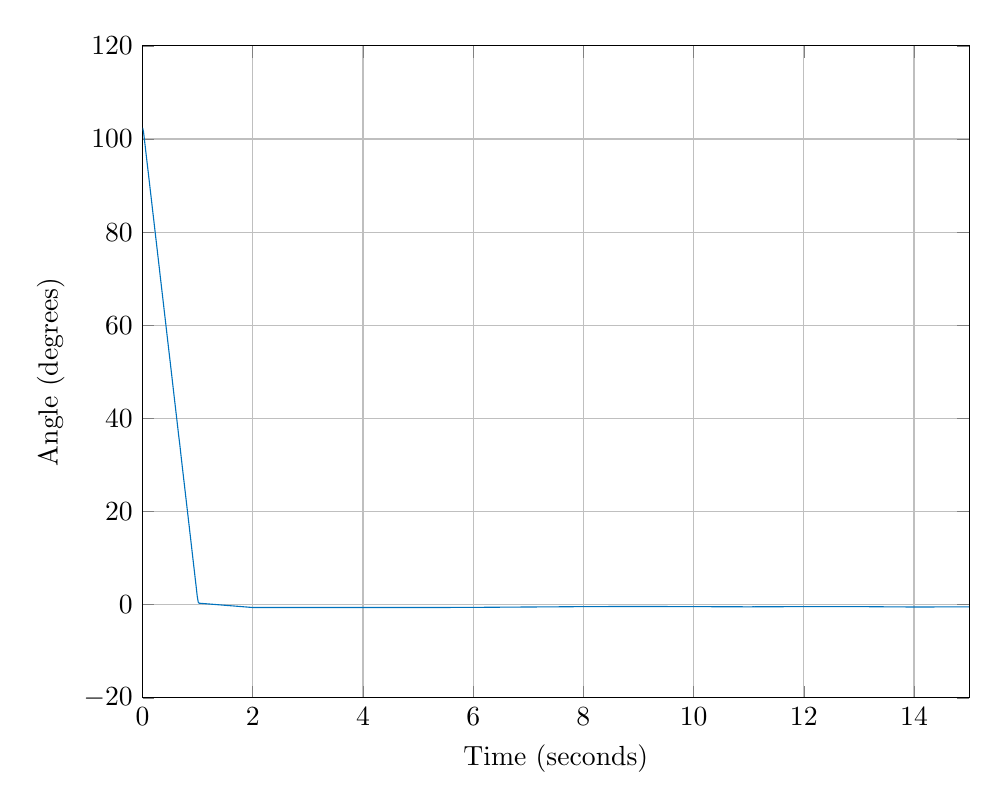
\begin{tikzpicture}

\begin{axis}[%
width=4.133in,
height=3.26in,
at={(0.693in,0.44in)},
scale only axis,
xmin=0,
xmax=15,
xmajorgrids,
xlabel={Time (seconds)},
ymin=-20,
ymax=120,
ymajorgrids,
ylabel={Angle (degrees)},
axis background/.style={fill=white}
]
\addplot [color=mycolor1,solid,forget plot]
  table[row sep=crcr]{%
0	102.4204\\
0.0174364199999999	101.5544\\
0.0324413389999997	100.0424\\
0.0480745519989999	98.4444\\
0.0640998179989997	96.7824\\
0.0802082269989997	95.1624\\
0.0962292989999996	93.5344\\
0.112140156998999	91.9224\\
0.128197941	90.2964\\
0.144129229999999	88.6344\\
0.160211415	87.0184\\
0.176086827998999	85.3564\\
0.192200153	83.7364\\
0.208225839	82.1044\\
0.224227045999	80.4664\\
0.240080554	78.8344\\
0.256212316	77.1944\\
0.272087498	75.5624\\
0.287968980998999	73.9284\\
0.304175280999999	72.2944\\
0.320220736	70.5924\\
0.336536562	68.9704\\
0.352217476999	67.3464\\
0.368193181	65.7424\\
0.384155161001	64.1064\\
0.400024181	62.4684\\
0.415951047999999	60.8544\\
0.431919778999	59.2064\\
0.447973876999999	57.5584\\
0.464059460999	55.9184\\
0.480058576	54.2984\\
0.496060176999	52.6744\\
0.512173605	51.0444\\
0.528068001999999	49.4124\\
0.544010151	47.7564\\
0.559998673	46.1064\\
0.576011581999999	44.4624\\
0.591989840999001	42.8464\\
0.608012696998999	41.1984\\
0.624180601999001	39.5624\\
0.640136015	37.9184\\
0.655922871	36.2824\\
0.674092178999	34.5824\\
0.689323626999999	32.9744\\
0.704526350000001	31.3604\\
0.720011259000001	29.7284\\
0.736073612999999	28.1104\\
0.752035972	26.4784\\
0.768029434998999	24.8544\\
0.784062675	23.2164\\
0.799996894999	21.5684\\
0.816036227998999	19.9424\\
0.832063142999	18.3104\\
0.848087181999999	16.6724\\
0.864017762999999	15.0324\\
0.880263498999	13.3904\\
0.896149981	11.7404\\
0.911956988998999	10.1104\\
0.928179579998999	8.45439999999999\\
0.944204442999999	6.81440000000001\\
0.960016884999	5.1844\\
0.976101866998999	3.5664\\
0.992018666999	1.87039999999999\\
1.010025436999	0.572399999999988\\
1.025319382	0.316400000000002\\
1.040847788	0.300399999999996\\
1.056282832	0.284399999999977\\
1.072203170999	0.27239999999999\\
1.088214014	0.256399999999985\\
1.10410021	0.240399999999994\\
1.120184143999	0.224399999999989\\
1.136192742999	0.212399999999974\\
1.153332650999	0.194400000000002\\
1.169049851999	0.180399999999992\\
1.184664222999	0.164400000000001\\
1.200207943999	0.148399999999995\\
1.216198867	0.136399999999981\\
1.232058714	0.120399999999989\\
1.248018682	0.104399999999984\\
1.264163278999	0.0884000000000071\\
1.280203778999	0.0723999999999876\\
1.296205294999	0.0583999999999776\\
1.312056418999	0.044399999999996\\
1.328273238999	0.0283999999999907\\
1.34413268	0.0123999999999853\\
1.36020774	-0.00360000000000582\\
1.376078550999	-0.0176000000000158\\
1.392107234999	-0.0315999999999974\\
1.408105734	-0.047600000000017\\
1.424191177	-0.0636000000000223\\
1.439961965999	-0.0795999999999992\\
1.455935304	-0.0936000000000092\\
1.47206816	-0.107600000000005\\
1.488172840999	-0.12360000000001\\
1.504562021999	-0.139600000000016\\
1.520175550999	-0.155600000000007\\
1.536107556	-0.171600000000012\\
1.552158274999	-0.183599999999998\\
1.568218684999	-0.199600000000004\\
1.584080896999	-0.215600000000023\\
1.600417683999	-0.2316\\
1.616165892999	-0.247600000000006\\
1.632020097999	-0.259600000000006\\
1.64800708	-0.275600000000011\\
1.663921684	-0.291600000000017\\
1.679974225	-0.307600000000008\\
1.696183247	-0.323600000000013\\
1.712205491999	-0.337600000000023\\
1.728202698	-0.351600000000005\\
1.74413995	-0.36760000000001\\
1.760297773	-0.383600000000001\\
1.776070962999	-0.399600000000007\\
1.792014729999	-0.413600000000017\\
1.808010689999	-0.427600000000012\\
1.824178137999	-0.443600000000018\\
1.840175485999	-0.459599999999995\\
1.856258517999	-0.475600000000014\\
1.872046412	-0.489600000000024\\
1.888057365999	-0.503600000000006\\
1.903962273	-0.519600000000011\\
1.920177224999	-0.535600000000002\\
1.936126995999	-0.551600000000008\\
1.952091072999	-0.565600000000018\\
1.968175580999	-0.579599999999999\\
1.984195162	-0.595600000000019\\
2.000203769999	-0.611599999999996\\
2.017723236	-0.61960000000002\\
2.03286175	-0.61960000000002\\
2.047944468	-0.61960000000002\\
2.063966206	-0.61960000000002\\
2.079946495999	-0.61960000000002\\
2.098116071999	-0.61960000000002\\
2.113148563999	-0.61960000000002\\
2.128386502	-0.61960000000002\\
2.144113648	-0.61960000000002\\
2.159934625999	-0.61960000000002\\
2.17611003	-0.61960000000002\\
2.19209383	-0.61960000000002\\
2.208082964	-0.61960000000002\\
2.224121148999	-0.61960000000002\\
2.240056938	-0.61960000000002\\
2.256037618	-0.61960000000002\\
2.274214714	-0.61960000000002\\
2.289394059	-0.61960000000002\\
2.30458258	-0.61960000000002\\
2.320164677999	-0.61960000000002\\
2.337081984	-0.61960000000002\\
2.35244274	-0.61960000000002\\
2.368217484	-0.61960000000002\\
2.384157628001	-0.61960000000002\\
2.400174926	-0.61960000000002\\
2.416436913	-0.61960000000002\\
2.432192117999	-0.61960000000002\\
2.448213056	-0.61960000000002\\
2.463979465	-0.61960000000002\\
2.480214109999	-0.61960000000002\\
2.496150904	-0.61960000000002\\
2.51202091	-0.61960000000002\\
2.528092401	-0.61960000000002\\
2.544057696	-0.61960000000002\\
2.560052073	-0.61960000000002\\
2.576022575	-0.61960000000002\\
2.592061983	-0.61960000000002\\
2.608066929	-0.61960000000002\\
2.624044757	-0.61960000000002\\
2.640132328999	-0.61960000000002\\
2.656117033999	-0.61960000000002\\
2.67206056	-0.61960000000002\\
2.688063049	-0.61960000000002\\
2.704059540999	-0.61960000000002\\
2.720050849	-0.61960000000002\\
2.736020509999	-0.61960000000002\\
2.752026533	-0.61960000000002\\
2.768011547999	-0.61960000000002\\
2.784059405999	-0.61960000000002\\
2.800047727999	-0.61960000000002\\
2.816122816999	-0.61960000000002\\
2.832212373999	-0.61960000000002\\
2.848164019	-0.61960000000002\\
2.864079035	-0.61960000000002\\
2.880064906999	-0.61960000000002\\
2.895952181999	-0.61960000000002\\
2.912846776	-0.61960000000002\\
2.928184557999	-0.61960000000002\\
2.944053722999	-0.61960000000002\\
2.960053562	-0.61960000000002\\
2.975999719	-0.61960000000002\\
2.994254925999	-0.61960000000002\\
3.008585559999	-0.61960000000002\\
3.024117377	-0.61960000000002\\
3.040093882999	-0.61960000000002\\
3.056201951999	-0.61960000000002\\
3.072171406	-0.61960000000002\\
3.088090247	-0.61960000000002\\
3.104069609	-0.61960000000002\\
3.120078504	-0.61960000000002\\
3.136031345001	-0.61960000000002\\
3.151960363999	-0.61960000000002\\
3.168030761999	-0.61960000000002\\
3.184088748	-0.61960000000002\\
3.200043123999	-0.61960000000002\\
3.216096242999	-0.61960000000002\\
3.232345321	-0.61960000000002\\
3.248246571	-0.61960000000002\\
3.264068767999	-0.61960000000002\\
3.280051673	-0.61960000000002\\
3.296060010999	-0.61960000000002\\
3.312053810999	-0.61960000000002\\
3.328149971999	-0.61960000000002\\
3.344134951999	-0.61960000000002\\
3.359977662999	-0.61960000000002\\
3.378183431	-0.61960000000002\\
3.393311515	-0.61960000000002\\
3.408329681	-0.61960000000002\\
3.423965118999	-0.61960000000002\\
3.440091207998	-0.61960000000002\\
3.456068635999	-0.61960000000002\\
3.472002359999	-0.61960000000002\\
3.488001425	-0.61960000000002\\
3.50399475	-0.61960000000002\\
3.520059731999	-0.61960000000002\\
3.536060682999	-0.61960000000002\\
3.552030617999	-0.61960000000002\\
3.568062920999	-0.61960000000002\\
3.584051137999	-0.61960000000002\\
3.600061967	-0.61960000000002\\
3.616100809	-0.61960000000002\\
3.632072217999	-0.61960000000002\\
3.648039532	-0.61960000000002\\
3.664712465999	-0.61960000000002\\
3.680096951	-0.61960000000002\\
3.695980576999	-0.61960000000002\\
3.712197562	-0.61960000000002\\
3.728204576999	-0.61960000000002\\
3.744034690999	-0.61960000000002\\
3.760202780999	-0.61960000000002\\
3.776177844	-0.61960000000002\\
3.792106691	-0.61960000000002\\
3.808257335999	-0.61960000000002\\
3.824203394	-0.61960000000002\\
3.840289837999	-0.61960000000002\\
3.856198254999	-0.61960000000002\\
3.872320295	-0.61960000000002\\
3.888010259	-0.61960000000002\\
3.903925231999	-0.61960000000002\\
3.920045058999	-0.61960000000002\\
3.936110399	-0.61960000000002\\
3.952102193	-0.61960000000002\\
3.967993017	-0.61960000000002\\
3.984011323	-0.61960000000002\\
4.000032677999	-0.61960000000002\\
4.017330059	-0.61960000000002\\
4.032641609	-0.61960000000002\\
4.048226707	-0.61960000000002\\
4.064199278999	-0.61960000000002\\
4.080152432999	-0.61960000000002\\
4.096619945999	-0.61960000000002\\
4.112303497	-0.61960000000002\\
4.128193923	-0.61960000000002\\
4.144085671	-0.61960000000002\\
4.159940774	-0.61960000000002\\
4.177991844	-0.61960000000002\\
4.192873846999	-0.61960000000002\\
4.208390108	-0.61960000000002\\
4.224197497	-0.61960000000002\\
4.240197639999	-0.61960000000002\\
4.256212827999	-0.61960000000002\\
4.272338436999	-0.61960000000002\\
4.288223765999	-0.61960000000002\\
4.304298875	-0.61960000000002\\
4.320226073999	-0.61960000000002\\
4.338806023	-0.61960000000002\\
4.35426679	-0.61960000000002\\
4.369876093999	-0.61960000000002\\
4.385399932999	-0.61960000000002\\
4.4010598	-0.61960000000002\\
4.416364753001	-0.61960000000002\\
4.432178811	-0.61960000000002\\
4.448292142	-0.61960000000002\\
4.464212710999	-0.61960000000002\\
4.480030828	-0.61960000000002\\
4.496202891	-0.61960000000002\\
4.512198484999	-0.61960000000002\\
4.528154323999	-0.61960000000002\\
4.544188686	-0.61960000000002\\
4.560194137999	-0.61960000000002\\
4.576274293	-0.61960000000002\\
4.592259242999	-0.61960000000002\\
4.608199813	-0.61960000000002\\
4.624300734999	-0.61960000000002\\
4.64027266	-0.61960000000002\\
4.656180592	-0.61960000000002\\
4.672191971	-0.61960000000002\\
4.688079760999	-0.61960000000002\\
4.704200662999	-0.61960000000002\\
4.720204184	-0.61960000000002\\
4.736184309999	-0.61960000000002\\
4.752069476999	-0.61960000000002\\
4.768200349	-0.61960000000002\\
4.784186788999	-0.61960000000002\\
4.800115549998	-0.61960000000002\\
4.816082899999	-0.61960000000002\\
4.832065785	-0.61960000000002\\
4.848044270999	-0.61960000000002\\
4.864202106999	-0.61960000000002\\
4.880229006999	-0.61960000000002\\
4.896204436	-0.61960000000002\\
4.912107910999	-0.61960000000002\\
4.928169884999	-0.61960000000002\\
4.944215616999	-0.61960000000002\\
4.960190734	-0.61960000000002\\
4.976067642	-0.61960000000002\\
4.992011913999	-0.61960000000002\\
5.009937497	-0.61960000000002\\
5.024994391998	-0.61960000000002\\
5.040080075	-0.61760000000001\\
5.056301701	-0.61760000000001\\
5.072096184999	-0.61760000000001\\
5.088119672	-0.615600000000015\\
5.1041215	-0.615600000000015\\
5.12031192	-0.615600000000015\\
5.136008354999	-0.613600000000019\\
5.152018478999	-0.613600000000019\\
5.168155486999	-0.613600000000019\\
5.184126971999	-0.611599999999996\\
5.200222323	-0.611599999999996\\
5.216202545999	-0.611599999999996\\
5.232202991999	-0.611599999999996\\
5.248138389	-0.6096\\
5.264081293999	-0.6096\\
5.280199671	-0.6096\\
5.296137108	-0.607600000000005\\
5.312170363	-0.607600000000005\\
5.328191163999	-0.607600000000005\\
5.344200639999	-0.60560000000001\\
5.360208571999	-0.60560000000001\\
5.37619716	-0.60560000000001\\
5.392456622	-0.6036\\
5.409543821999	-0.6036\\
5.425040842999	-0.6036\\
5.440446882	-0.601600000000005\\
5.456213241	-0.601600000000005\\
5.472084109	-0.601600000000005\\
5.488205918	-0.599600000000009\\
5.504746311	-0.599600000000009\\
5.520214770999	-0.599600000000009\\
5.536072732	-0.599600000000009\\
5.552104776	-0.597600000000014\\
5.568203873	-0.597600000000014\\
5.584268137999	-0.597600000000014\\
5.600219861999	-0.595600000000019\\
5.616093009	-0.595600000000019\\
5.63218009	-0.595600000000019\\
5.648047674	-0.593600000000009\\
5.663950050999	-0.593600000000009\\
5.680101163999	-0.593600000000009\\
5.696208217	-0.591600000000014\\
5.712189446999	-0.591600000000014\\
5.728124238	-0.591600000000014\\
5.744016382999	-0.589600000000019\\
5.759969333	-0.589600000000019\\
5.776390062	-0.589600000000019\\
5.792203684	-0.587599999999995\\
5.808111793	-0.587599999999995\\
5.824230427999	-0.587599999999995\\
5.840264067999	-0.585599999999999\\
5.85619913	-0.585599999999999\\
5.872219665999	-0.585599999999999\\
5.888061250999	-0.585599999999999\\
5.904005122	-0.583600000000004\\
5.920174464999	-0.583600000000004\\
5.936176504	-0.583600000000004\\
5.952099142	-0.581600000000009\\
5.968218316999	-0.581600000000009\\
5.984208788999	-0.581600000000009\\
6.000112769999	-0.579599999999999\\
6.017582649	-0.579599999999999\\
6.032675724	-0.579599999999999\\
6.04809412	-0.575600000000009\\
6.064063339999	-0.575600000000009\\
6.080053071	-0.575600000000009\\
6.096028728999	-0.571599999999989\\
6.112248274999	-0.571599999999989\\
6.128208428999	-0.571599999999989\\
6.14396666	-0.569599999999994\\
6.159953748999	-0.567599999999999\\
6.176064281	-0.567599999999999\\
6.192075689999	-0.567599999999999\\
6.208060142999	-0.563599999999994\\
6.224060497999	-0.563599999999994\\
6.240172138999	-0.563599999999994\\
6.256208938	-0.559600000000003\\
6.272330718	-0.559600000000003\\
6.288081672	-0.559600000000003\\
6.30405878	-0.555599999999998\\
6.320175488	-0.555599999999998\\
6.336359641	-0.555599999999998\\
6.352202451999	-0.551600000000008\\
6.368325165	-0.551600000000008\\
6.384229085999	-0.551600000000008\\
6.399927596999	-0.547600000000017\\
6.418094974999	-0.547600000000017\\
6.433175913	-0.547600000000017\\
6.448245408999	-0.545600000000007\\
6.464020657999	-0.543599999999998\\
6.480112335999	-0.543599999999998\\
6.496167585	-0.541599999999988\\
6.512213201999	-0.539599999999993\\
6.528219730999	-0.539599999999993\\
6.544099521999	-0.539599999999993\\
6.560153358	-0.535600000000002\\
6.576187239	-0.535600000000002\\
6.591977611	-0.535600000000002\\
6.608326035999	-0.531599999999997\\
6.624058384	-0.531599999999997\\
6.640218780999	-0.531599999999997\\
6.655994672	-0.527600000000007\\
6.672041295999	-0.527600000000007\\
6.688202523	-0.527600000000007\\
6.704048743999	-0.523600000000016\\
6.720080634999	-0.523600000000016\\
6.736160679	-0.523600000000016\\
6.752048283	-0.519599999999997\\
6.768064769999	-0.519599999999997\\
6.784071057999	-0.519599999999997\\
6.800020132	-0.517599999999987\\
6.816298351	-0.515599999999992\\
6.832204156999	-0.515599999999992\\
6.848177184999	-0.515599999999992\\
6.864213294999	-0.511600000000001\\
6.880201443	-0.511600000000001\\
6.896166096999	-0.511600000000001\\
6.911979625999	-0.507599999999996\\
6.92806041	-0.507599999999996\\
6.944051668999	-0.507599999999996\\
6.960060702999	-0.503600000000006\\
6.976001891	-0.503600000000006\\
6.992188637	-0.503600000000006\\
7.009917887999	-0.499600000000015\\
7.025062535	-0.499600000000015\\
7.040364753001	-0.499600000000015\\
7.056003098	-0.495599999999996\\
7.072091451999	-0.495599999999996\\
7.088046931	-0.495599999999996\\
7.104099507999	-0.493599999999986\\
7.120061782	-0.491599999999991\\
7.136064551999	-0.491599999999991\\
7.151995634999	-0.489599999999996\\
7.170209929999	-0.4876\\
7.185489417	-0.4876\\
7.200828347999	-0.4876\\
7.21612082	-0.483599999999996\\
7.232095876999	-0.483599999999996\\
7.248067061	-0.483599999999996\\
7.264062109	-0.479600000000005\\
7.280057412	-0.479600000000005\\
7.296058128001	-0.479600000000005\\
7.312066129999	-0.475600000000014\\
7.328052112	-0.475600000000014\\
7.344019281	-0.475600000000014\\
7.359993398999	-0.471599999999995\\
7.376050155	-0.471599999999995\\
7.392077826999	-0.471599999999995\\
7.407967070999	-0.46759999999999\\
7.424091946999	-0.46759999999999\\
7.440058199	-0.46759999999999\\
7.456025599	-0.465599999999995\\
7.472217814	-0.4636\\
7.488063783999	-0.4636\\
7.504063803	-0.4636\\
7.520128848999	-0.459599999999995\\
7.536059997	-0.459599999999995\\
7.552213804999	-0.459599999999995\\
7.568210811999	-0.455600000000004\\
7.584116689999	-0.455600000000004\\
7.600213226	-0.455600000000004\\
7.616205160999	-0.451600000000013\\
7.632079521	-0.451600000000013\\
7.647950417	-0.451600000000013\\
7.666106786001	-0.447600000000008\\
7.681468854999	-0.447600000000008\\
7.696943389	-0.447600000000008\\
7.712615464	-0.443599999999989\\
7.728273618999	-0.443599999999989\\
7.744215101	-0.443599999999989\\
7.760236634	-0.441599999999994\\
7.776114829999	-0.439599999999999\\
7.792352809999	-0.439599999999999\\
7.808138939999	-0.437600000000003\\
7.824086795999	-0.435599999999994\\
7.840110754	-0.435599999999994\\
7.856078049	-0.435599999999994\\
7.872126637999	-0.431600000000003\\
7.888043507999	-0.431600000000003\\
7.903946002	-0.431600000000003\\
7.920086553999	-0.427600000000012\\
7.936316118	-0.427600000000012\\
7.952195795	-0.427600000000012\\
7.968162714	-0.423600000000008\\
7.984209183	-0.423600000000008\\
8.000211878001	-0.423600000000008\\
8.016028740999	-0.421600000000012\\
8.032065369	-0.421600000000012\\
8.048202825	-0.421600000000012\\
8.064173947999	-0.419600000000017\\
8.080183639	-0.419600000000017\\
8.096363681	-0.419600000000017\\
8.11214023	-0.417600000000022\\
8.128158209	-0.417600000000022\\
8.144422215999	-0.417600000000022\\
8.160094943999	-0.417600000000022\\
8.176183418	-0.415600000000012\\
8.192197979999	-0.415600000000012\\
8.208134901999	-0.415600000000012\\
8.224202899999	-0.413600000000017\\
8.240206561999	-0.413600000000017\\
8.256082894999	-0.413600000000017\\
8.272055693	-0.411600000000021\\
8.288083318999	-0.411600000000021\\
8.304080361999	-0.411600000000021\\
8.320199710999	-0.409599999999998\\
8.336408568	-0.409599999999998\\
8.352774370999	-0.409599999999998\\
8.368230387	-0.407600000000002\\
8.384177747	-0.407600000000002\\
8.400262842	-0.407600000000002\\
8.416117839999	-0.405600000000007\\
8.431974916	-0.405600000000007\\
8.448092601999	-0.405600000000007\\
8.464086698	-0.403600000000012\\
8.480081342999	-0.403600000000012\\
8.496115599999	-0.403600000000012\\
8.512198596999	-0.403600000000012\\
8.528179257	-0.401600000000002\\
8.544071862999	-0.401600000000002\\
8.560199276	-0.401600000000002\\
8.576202712	-0.399600000000007\\
8.592157599999	-0.399600000000007\\
8.608204613999	-0.399600000000007\\
8.624250753001	-0.397600000000011\\
8.640201991999	-0.397600000000011\\
8.655952028	-0.397600000000011\\
8.674264316	-0.395600000000016\\
8.690029313	-0.395600000000016\\
8.70533116	-0.395600000000016\\
8.720462252	-0.393600000000021\\
8.736054311	-0.393600000000021\\
8.752167026	-0.393600000000021\\
8.768216337	-0.391600000000011\\
8.784117234999	-0.391600000000011\\
8.800222247999	-0.391600000000011\\
8.816085878001	-0.391600000000011\\
8.832200255999	-0.389600000000016\\
8.848208899999	-0.389600000000016\\
8.864074028	-0.389600000000016\\
8.879972388999	-0.38760000000002\\
8.898176418999	-0.38760000000002\\
8.913392229999	-0.38760000000002\\
8.92820018	-0.385600000000025\\
8.944193965	-0.385600000000025\\
8.960134269	-0.385600000000025\\
8.976188917	-0.383600000000001\\
8.99227928	-0.383600000000001\\
9.010184870999	-0.383600000000001\\
9.02539478	-0.385599999999997\\
9.040911420999	-0.385599999999997\\
9.056161129	-0.385599999999997\\
9.072005068999	-0.387599999999992\\
9.088078109	-0.387599999999992\\
9.104068896999	-0.387599999999992\\
9.120023436	-0.389600000000002\\
9.136077655	-0.389600000000002\\
9.151989933	-0.389600000000002\\
9.168026231	-0.389600000000002\\
9.184192672	-0.391599999999997\\
9.200145398999	-0.391599999999997\\
9.216075017999	-0.391599999999997\\
9.232121800999	-0.393599999999992\\
9.248089691999	-0.393599999999992\\
9.264096814999	-0.393599999999992\\
9.280090168	-0.395600000000016\\
9.295993071999	-0.395600000000016\\
9.314136978	-0.395600000000016\\
9.329233987	-0.397600000000011\\
9.344568609999	-0.397600000000011\\
9.360134695	-0.397600000000011\\
9.376179540999	-0.399600000000007\\
9.392306382	-0.399600000000007\\
9.407975764	-0.399600000000007\\
9.424032971	-0.401600000000002\\
9.440175618	-0.401600000000002\\
9.456204844	-0.401600000000002\\
9.47216182	-0.401600000000002\\
9.488058073999	-0.403600000000012\\
9.504047424	-0.403600000000012\\
9.520006595001	-0.403600000000012\\
9.536055745999	-0.405600000000007\\
9.552117752999	-0.405600000000007\\
9.568094486	-0.405600000000007\\
9.584199884999	-0.407600000000002\\
9.600003557	-0.407600000000002\\
9.615998725	-0.407600000000002\\
9.632118151999	-0.409599999999998\\
9.648181718999	-0.409599999999998\\
9.6641735	-0.409599999999998\\
9.680241717999	-0.411599999999993\\
9.696210542	-0.411599999999993\\
9.712220362999	-0.411599999999993\\
9.728217976	-0.413600000000002\\
9.744161601999	-0.413600000000002\\
9.760112507	-0.413600000000002\\
9.776056043999	-0.415599999999998\\
9.792012257	-0.415599999999998\\
9.807986535	-0.415599999999998\\
9.824083686	-0.415599999999998\\
9.840049543	-0.417599999999993\\
9.856053837	-0.417599999999993\\
9.87206002	-0.417599999999993\\
9.888050457	-0.419599999999988\\
9.903937345001	-0.419599999999988\\
9.922163447	-0.419599999999988\\
9.937634653	-0.421600000000012\\
9.953129364	-0.421600000000012\\
9.968507009	-0.421600000000012\\
9.984406637999	-0.423600000000008\\
10.000217073	-0.423600000000008\\
10.017969955	-0.423600000000008\\
10.033488119999	-0.425600000000003\\
10.048571818	-0.425600000000003\\
10.064066002	-0.425600000000003\\
10.080080618999	-0.427600000000012\\
10.096186568	-0.427600000000012\\
10.112210625999	-0.427600000000012\\
10.128145726	-0.429600000000008\\
10.144204910999	-0.429600000000008\\
10.159938590999	-0.429600000000008\\
10.176176891	-0.429600000000008\\
10.192216039	-0.431600000000003\\
10.208161094	-0.431600000000003\\
10.224046457	-0.431600000000003\\
10.240191195	-0.433599999999998\\
10.25609008	-0.433599999999998\\
10.272064229999	-0.433599999999998\\
10.288082545999	-0.435599999999994\\
10.304050887999	-0.435599999999994\\
10.319991915999	-0.435599999999994\\
10.336056162999	-0.437600000000003\\
10.352059774999	-0.437600000000003\\
10.368178226999	-0.437600000000003\\
10.384231177	-0.439599999999999\\
10.400195154	-0.439599999999999\\
10.416024529	-0.439599999999999\\
10.432109223999	-0.441599999999994\\
10.448068096	-0.441599999999994\\
10.464246115	-0.441599999999994\\
10.480207807999	-0.441599999999994\\
10.496232162	-0.443599999999989\\
10.512324549998	-0.443599999999989\\
10.528215467	-0.443599999999989\\
10.544222823	-0.445600000000013\\
10.560126141	-0.445600000000013\\
10.576121762	-0.445600000000013\\
10.592047838	-0.447600000000008\\
10.608060882	-0.447600000000008\\
10.624047891998	-0.447600000000008\\
10.640089960999	-0.449600000000004\\
10.656113156999	-0.449600000000004\\
10.672093887999	-0.449600000000004\\
10.688308031999	-0.451600000000013\\
10.704151377	-0.451600000000013\\
10.720198939	-0.451600000000013\\
10.736174438	-0.453600000000009\\
10.752210641	-0.453600000000009\\
10.768198273	-0.453600000000009\\
10.784261927	-0.455600000000004\\
10.800130243999	-0.455600000000004\\
10.816293451	-0.455600000000004\\
10.832309474	-0.455600000000004\\
10.848255181	-0.457599999999999\\
10.864332035999	-0.457599999999999\\
10.880404217999	-0.457599999999999\\
10.896335146999	-0.459599999999995\\
10.911954291	-0.459599999999995\\
10.92818571	-0.459599999999995\\
10.943977613999	-0.461600000000004\\
10.960189547999	-0.461600000000004\\
10.976184509999	-0.461600000000004\\
10.992134073999	-0.4636\\
11.008082330999	-0.461600000000004\\
11.024231929	-0.459599999999995\\
11.040197245	-0.459599999999995\\
11.056075523	-0.461600000000004\\
11.072125294999	-0.457599999999999\\
11.088084674	-0.457599999999999\\
11.104015208999	-0.459599999999995\\
11.120054285999	-0.455600000000004\\
11.136115278	-0.455600000000004\\
11.152140017	-0.457599999999999\\
11.167985531999	-0.455600000000004\\
11.184181004	-0.453600000000009\\
11.200179856	-0.455600000000004\\
11.216176351999	-0.453600000000009\\
11.23215628	-0.451600000000013\\
11.248217498	-0.453600000000009\\
11.26421231	-0.451600000000013\\
11.280067560999	-0.44959999999999\\
11.296085229999	-0.44959999999999\\
11.312042231999	-0.449600000000004\\
11.328179461999	-0.447600000000008\\
11.3446142	-0.447600000000008\\
11.360203604	-0.449600000000004\\
11.376146488	-0.445600000000013\\
11.392205656999	-0.445600000000013\\
11.407981149	-0.447600000000008\\
11.423929568999	-0.443599999999989\\
11.440186409	-0.443599999999989\\
11.456194918999	-0.445599999999985\\
11.472014035	-0.443599999999989\\
11.488117798	-0.441599999999994\\
11.504316311999	-0.443599999999989\\
11.520250436	-0.441599999999994\\
11.536185748	-0.439599999999999\\
11.552139262	-0.441599999999994\\
11.568174371	-0.439599999999999\\
11.584267846	-0.437600000000003\\
11.600248576999	-0.437600000000003\\
11.616204946999	-0.437600000000003\\
11.63221312	-0.435599999999994\\
11.648209941	-0.435599999999994\\
11.663996004	-0.435599999999994\\
11.680128519999	-0.433599999999998\\
11.696163823999	-0.433599999999998\\
11.712303564999	-0.435599999999994\\
11.728084547	-0.431600000000003\\
11.744057790999	-0.431600000000003\\
11.760244778	-0.433599999999998\\
11.776229196999	-0.429600000000008\\
11.792264014999	-0.429600000000008\\
11.808331186	-0.431600000000003\\
11.825191298	-0.427600000000012\\
11.840621656999	-0.427600000000012\\
11.856223063	-0.429600000000008\\
11.872230283999	-0.427600000000012\\
11.888200314999	-0.425599999999989\\
11.904167559999	-0.427599999999984\\
11.920138774	-0.425599999999989\\
11.936170007999	-0.423599999999993\\
11.952202912	-0.425600000000003\\
11.968161111	-0.423600000000008\\
11.984070997	-0.421600000000012\\
12.000056677999	-0.421600000000012\\
12.017315042	-0.423600000000008\\
12.032281806	-0.423600000000008\\
12.048081410999	-0.423600000000008\\
12.064308474	-0.423600000000008\\
12.080278104	-0.423600000000008\\
12.096073921	-0.423600000000008\\
12.112073715	-0.423600000000008\\
12.128202931	-0.423600000000008\\
12.144180404	-0.423600000000008\\
12.160081519	-0.423600000000008\\
12.176206906999	-0.423600000000008\\
12.192068107	-0.423600000000008\\
12.208199363	-0.423600000000008\\
12.22407479	-0.423600000000008\\
12.240057064	-0.423600000000008\\
12.256054823	-0.423600000000008\\
12.2720362	-0.423600000000008\\
12.288030491	-0.423600000000008\\
12.304027457998	-0.423600000000008\\
12.320016186999	-0.423600000000008\\
12.336050924	-0.423600000000008\\
12.352062083	-0.423600000000008\\
12.368033031999	-0.423600000000008\\
12.384199802999	-0.423600000000008\\
12.400176484999	-0.423600000000008\\
12.415988171999	-0.423600000000008\\
12.432075977999	-0.423600000000008\\
12.448216396999	-0.423600000000008\\
12.464242686	-0.423600000000008\\
12.480121139	-0.423600000000008\\
12.496033755	-0.423600000000008\\
12.512193856999	-0.423600000000008\\
12.528225082	-0.423600000000008\\
12.544176526	-0.423600000000008\\
12.560273396	-0.423600000000008\\
12.576195802999	-0.423600000000008\\
12.592181449	-0.423600000000008\\
12.608272439999	-0.423600000000008\\
12.624093889	-0.423600000000008\\
12.640066861999	-0.423600000000008\\
12.6559628	-0.423600000000008\\
12.672079446999	-0.423600000000008\\
12.688097774	-0.423600000000008\\
12.704333130999	-0.423600000000008\\
12.720306903	-0.423600000000008\\
12.736221915	-0.423600000000008\\
12.752089722999	-0.423600000000008\\
12.768073213	-0.423600000000008\\
12.783995431	-0.423600000000008\\
12.800007804999	-0.423600000000008\\
12.816050023	-0.423600000000008\\
12.83209339	-0.423600000000008\\
12.848042714	-0.423600000000008\\
12.864146927	-0.423600000000008\\
12.880118554	-0.423600000000008\\
12.896110917	-0.423600000000008\\
12.91206448	-0.423600000000008\\
12.928080915999	-0.423600000000008\\
12.944202627	-0.423600000000008\\
12.960184784	-0.423600000000008\\
12.976024661001	-0.423600000000008\\
12.992227343999	-0.423600000000008\\
13.010088955	-0.423600000000008\\
13.025480401	-0.423600000000008\\
13.040947026	-0.427600000000012\\
13.056400221999	-0.427600000000012\\
13.072421052999	-0.427600000000012\\
13.088182045999	-0.429600000000008\\
13.104083917	-0.431600000000003\\
13.120068872	-0.431600000000003\\
13.13606193	-0.433599999999998\\
13.152128434999	-0.435599999999994\\
13.168114924	-0.435599999999994\\
13.184053543	-0.435599999999994\\
13.200015246	-0.439600000000013\\
13.216070555	-0.439600000000013\\
13.232188236	-0.439600000000013\\
13.248141116999	-0.443600000000018\\
13.26421102	-0.443600000000018\\
13.280210879	-0.443600000000018\\
13.296234049998	-0.447600000000008\\
13.312201075	-0.447600000000008\\
13.328236222999	-0.447600000000008\\
13.344222486	-0.451600000000013\\
13.360206333999	-0.451600000000013\\
13.376192356	-0.451600000000013\\
13.392119818999	-0.455600000000004\\
13.407962903999	-0.455600000000004\\
13.426396255999	-0.455600000000004\\
13.441892443	-0.457599999999999\\
13.457407142999	-0.459599999999995\\
13.472815811999	-0.459599999999995\\
13.488056892999	-0.461600000000004\\
13.504058335	-0.4636\\
13.520110141	-0.4636\\
13.536202068	-0.4636\\
13.552206391998	-0.46759999999999\\
13.568088538999	-0.46759999999999\\
13.584002033999	-0.46759999999999\\
13.600041446	-0.471600000000009\\
13.616008505	-0.471600000000009\\
13.631974613999	-0.471600000000009\\
13.648012806	-0.475600000000014\\
13.663901446999	-0.475600000000014\\
13.680061205	-0.475600000000014\\
13.69632314	-0.479600000000005\\
13.712179460999	-0.479600000000005\\
13.728084750999	-0.479600000000005\\
13.743986149999	-0.4816\\
13.760055311999	-0.483599999999996\\
13.776062998999	-0.483599999999996\\
13.792184378001	-0.485600000000005\\
13.808313684999	-0.487600000000015\\
13.824265479999	-0.487600000000015\\
13.840226965999	-0.487600000000015\\
13.856213990999	-0.49160000000002\\
13.872097174998	-0.49160000000002\\
13.888206016	-0.49160000000002\\
13.904039655	-0.49560000000001\\
13.919964221	-0.49560000000001\\
13.936103005	-0.49560000000001\\
13.952180613999	-0.499600000000015\\
13.968192709	-0.499600000000015\\
13.984070132	-0.499600000000015\\
14.000051488999	-0.503600000000006\\
14.016011151999	-0.503600000000006\\
14.034246443999	-0.50160000000001\\
14.049343563	-0.50160000000001\\
14.064405297	-0.50160000000001\\
14.080171981999	-0.499600000000015\\
14.096061645999	-0.499600000000015\\
14.112229215	-0.499600000000015\\
14.128208261	-0.497599999999991\\
14.144170935999	-0.497599999999991\\
14.160048948999	-0.497599999999991\\
14.17606949	-0.495599999999996\\
14.192172597	-0.495599999999996\\
14.208240257	-0.495599999999996\\
14.224071500999	-0.495599999999996\\
14.240099358	-0.493599999999986\\
14.256054384999	-0.493599999999986\\
14.27218038	-0.493599999999986\\
14.288206633	-0.491599999999991\\
14.304213702999	-0.491599999999991\\
14.320425275999	-0.491599999999991\\
14.33652227	-0.489599999999996\\
14.352191584999	-0.489599999999996\\
14.368370188	-0.489599999999996\\
14.384222978999	-0.4876\\
14.400103646999	-0.4876\\
14.416020157999	-0.4876\\
14.431916567	-0.485600000000005\\
14.448193839	-0.485600000000005\\
14.464190675999	-0.485600000000005\\
14.480051981	-0.483599999999996\\
14.496002953999	-0.483599999999996\\
14.512052755999	-0.483599999999996\\
14.528050965999	-0.483599999999996\\
14.544508546	-0.4816\\
14.560222451999	-0.4816\\
14.576060674998	-0.4816\\
14.592227091	-0.479600000000005\\
14.6082781	-0.479600000000005\\
14.624190004999	-0.479600000000005\\
14.640100294999	-0.47760000000001\\
14.655963758	-0.47760000000001\\
14.67435481	-0.47760000000001\\
14.689904813	-0.475600000000014\\
14.705240781999	-0.475600000000014\\
14.720675092999	-0.475600000000014\\
14.7361544	-0.473600000000005\\
14.752174096	-0.473600000000005\\
14.768177503001	-0.473600000000005\\
14.784122136999	-0.471600000000009\\
14.800116461	-0.471600000000009\\
14.816190267999	-0.471600000000009\\
14.83196707	-0.469600000000014\\
14.847890165	-0.469600000000014\\
14.866124297	-0.469600000000014\\
14.881334130999	-0.467600000000019\\
14.896480326	-0.467600000000019\\
14.911933860999	-0.467600000000019\\
14.928071076999	-0.467600000000019\\
14.944316551999	-0.465600000000023\\
14.960207469	-0.465600000000023\\
14.9761995	-0.465600000000023\\
14.992234368	-0.463600000000014\\
15.008099286001	-0.461600000000018\\
15.024100913	-0.461600000000018\\
15.040066068999	-0.459600000000023\\
15.056057943999	-0.459600000000023\\
15.072058004	-0.457600000000028\\
15.088056785	-0.455600000000032\\
15.103969566	-0.455600000000032\\
15.120139771999	-0.453600000000023\\
15.136092712999	-0.451600000000013\\
15.152243794999	-0.451600000000013\\
15.168113941999	-0.44959999999999\\
15.184102256999	-0.44959999999999\\
15.200057688	-0.447599999999994\\
15.216106825	-0.445599999999985\\
15.232155876	-0.445599999999985\\
15.248052339999	-0.443599999999989\\
15.264006459	-0.441599999999994\\
15.280059804999	-0.441599999999994\\
15.296075844999	-0.439599999999999\\
15.312006465	-0.437600000000003\\
15.328084943999	-0.437600000000003\\
15.344091292	-0.435599999999994\\
15.360216309	-0.435599999999994\\
15.376174509	-0.433599999999998\\
15.392242703	-0.431600000000003\\
15.408148096999	-0.431600000000003\\
15.424129934999	-0.429600000000008\\
15.440208695999	-0.427600000000012\\
15.456158507999	-0.427600000000012\\
15.472113941	-0.425600000000003\\
15.488208599	-0.423600000000008\\
15.504318838	-0.423600000000008\\
15.520073346	-0.421600000000012\\
15.53606457	-0.421600000000012\\
15.552151961999	-0.419600000000017\\
15.568169015	-0.417600000000022\\
15.584234967	-0.417600000000022\\
15.599992284999	-0.415600000000012\\
15.616203329999	-0.413600000000017\\
15.632208891	-0.413600000000017\\
15.648360293999	-0.411600000000021\\
15.663979619999	-0.411600000000021\\
15.680206142	-0.409600000000026\\
15.696039139999	-0.407600000000031\\
15.712021123	-0.407600000000031\\
15.728025839999	-0.405600000000021\\
15.743955066999	-0.403600000000026\\
15.759945672	-0.403600000000026\\
15.775934901999	-0.40160000000003\\
15.791938962999	-0.399600000000007\\
15.808067960999	-0.399600000000007\\
15.824084071999	-0.397599999999983\\
15.840209351999	-0.397599999999983\\
15.856185299	-0.395599999999988\\
15.872097137999	-0.393599999999992\\
15.888054205	-0.393599999999992\\
15.904087638	-0.391599999999997\\
15.92043274	-0.389600000000002\\
15.93625657	-0.389600000000002\\
15.951973564999	-0.387599999999992\\
15.96808757	-0.385599999999997\\
15.984078196	-0.385599999999997\\
16.000076363	-0.383600000000001\\
16.017419304999	-0.383600000000001\\
16.032518945	-0.381600000000006\\
16.048038115	-0.383600000000001\\
16.064179457	-0.383600000000001\\
16.080089608	-0.381600000000006\\
16.096209745	-0.381600000000006\\
16.112211828	-0.383600000000001\\
16.128254844999	-0.381600000000006\\
16.144377260999	-0.381600000000006\\
16.160760855999	-0.383600000000001\\
16.176029596999	-0.381600000000006\\
16.192246071	-0.381600000000006\\
16.208142510999	-0.383600000000001\\
16.224105165	-0.381600000000006\\
16.240195369	-0.381600000000006\\
16.256334673	-0.383600000000001\\
16.272221095001	-0.381600000000006\\
16.288179379	-0.381600000000006\\
16.304288576	-0.383600000000001\\
16.320204278999	-0.383600000000001\\
16.336513197	-0.381600000000006\\
16.352202608	-0.383600000000001\\
16.368166186	-0.383600000000001\\
16.384195255	-0.381600000000006\\
16.400215299	-0.383600000000001\\
16.415930625999	-0.383600000000001\\
16.434085879	-0.381600000000006\\
16.449159906	-0.381600000000006\\
16.464250705	-0.383600000000001\\
16.480304991999	-0.381600000000006\\
16.496220203999	-0.381600000000006\\
16.512202151999	-0.383600000000001\\
16.528101413	-0.381600000000006\\
16.544149997	-0.381600000000006\\
16.560065990999	-0.383600000000001\\
16.576004956	-0.381600000000006\\
16.592207549	-0.381600000000006\\
16.608268257	-0.383600000000001\\
16.624206891	-0.381600000000006\\
16.640209846999	-0.381600000000006\\
16.656037902999	-0.383600000000001\\
16.672152906	-0.383600000000001\\
16.688111431	-0.381600000000006\\
16.703996625	-0.383600000000001\\
16.720035247	-0.383600000000001\\
16.736058547999	-0.381600000000006\\
16.752113936999	-0.381600000000006\\
16.768028186999	-0.383600000000001\\
16.784013280999	-0.381600000000006\\
16.800015794	-0.381600000000006\\
16.816002217	-0.383600000000001\\
16.834184498	-0.381600000000006\\
16.849542337	-0.381600000000006\\
16.86514662	-0.383600000000001\\
16.880608941	-0.381600000000006\\
16.896201738	-0.381600000000006\\
16.911969179999	-0.383600000000001\\
16.928140903	-0.381600000000006\\
16.944346658	-0.381600000000006\\
16.960062028	-0.383600000000001\\
16.976220510999	-0.383600000000001\\
16.992099214	-0.381600000000006\\
17.010168516	-0.383600000000001\\
17.025185532999	-0.383600000000001\\
17.040385821	-0.383600000000001\\
17.056119436	-0.385599999999997\\
17.072188115999	-0.385599999999997\\
17.088083208	-0.385599999999997\\
17.104207006999	-0.385599999999997\\
17.120221293	-0.387599999999992\\
17.136083530999	-0.387599999999992\\
17.15214324	-0.387599999999992\\
17.16807357	-0.389600000000002\\
17.184080165	-0.389600000000002\\
17.200181538999	-0.389600000000002\\
17.216337696999	-0.391600000000011\\
17.23219012	-0.391600000000011\\
17.248209078	-0.391600000000011\\
17.264244281999	-0.393600000000021\\
17.280027134	-0.393600000000021\\
17.296024139999	-0.393600000000021\\
17.312150650999	-0.395600000000016\\
17.328212055	-0.395600000000016\\
17.344199089	-0.395600000000016\\
17.360207116999	-0.397600000000011\\
17.376113889999	-0.397600000000011\\
17.392192833	-0.397600000000011\\
17.408053314	-0.397600000000011\\
17.424054240999	-0.399600000000007\\
17.440178337	-0.399600000000007\\
17.456210342999	-0.399600000000007\\
17.472166632999	-0.401600000000002\\
17.488195597999	-0.401600000000002\\
17.504290026	-0.401600000000002\\
17.520261318	-0.403600000000012\\
17.536259675	-0.403600000000012\\
17.552192686999	-0.403600000000012\\
17.568225189999	-0.405600000000007\\
17.584186826999	-0.405600000000007\\
17.600209372	-0.405600000000007\\
17.616128137	-0.407600000000031\\
17.632078518	-0.407600000000031\\
17.648137262	-0.407600000000031\\
17.664111214	-0.409600000000026\\
17.680090593	-0.409600000000026\\
17.696108155	-0.409600000000026\\
17.711989486999	-0.409600000000026\\
17.727963122	-0.411600000000021\\
17.744046546	-0.411600000000021\\
17.760160955999	-0.411600000000021\\
17.776186971	-0.413600000000017\\
17.792073266998	-0.413600000000017\\
17.808062762999	-0.413600000000017\\
17.824009902	-0.415600000000012\\
17.840177325	-0.415600000000012\\
17.856101064999	-0.415600000000012\\
17.87219813	-0.417600000000022\\
17.888239929	-0.417600000000022\\
17.90405463	-0.417600000000022\\
17.920141925	-0.419600000000017\\
17.93616883	-0.419600000000017\\
17.952186323	-0.419600000000017\\
17.968221021999	-0.421600000000012\\
17.984175643	-0.421600000000012\\
18.000254143999	-0.421600000000012\\
18.018006172	-0.423600000000008\\
18.033270458999	-0.423600000000008\\
18.048769523999	-0.423600000000008\\
18.064204693	-0.423600000000008\\
18.080065582	-0.423600000000008\\
18.096057217999	-0.423600000000008\\
18.112165546999	-0.423600000000008\\
18.128240976999	-0.423600000000008\\
18.144070955999	-0.423600000000008\\
18.160050484	-0.423600000000008\\
18.176161663	-0.423600000000008\\
18.192220056	-0.423600000000008\\
18.208210718	-0.423600000000008\\
18.224198965999	-0.423600000000008\\
18.240155497999	-0.423600000000008\\
18.256261616999	-0.423600000000008\\
18.272199965	-0.423600000000008\\
18.28810054	-0.423600000000008\\
18.304180894999	-0.423600000000008\\
18.32028266	-0.423600000000008\\
18.336715047999	-0.423600000000008\\
18.352196646999	-0.423600000000008\\
18.368243302	-0.423600000000008\\
18.384243356999	-0.423600000000008\\
18.400204653	-0.423600000000008\\
18.415964153	-0.423600000000008\\
18.432162104999	-0.423600000000008\\
18.448199002	-0.423600000000008\\
18.464213693999	-0.423600000000008\\
18.480082736999	-0.423600000000008\\
18.496054085999	-0.423600000000008\\
18.512329413999	-0.423600000000008\\
18.528374281999	-0.423600000000008\\
18.544215648	-0.423600000000008\\
18.560206361999	-0.423600000000008\\
18.576181063999	-0.423600000000008\\
18.592086497999	-0.423600000000008\\
18.60805443	-0.423600000000008\\
18.624091668	-0.423600000000008\\
18.640203531	-0.423600000000008\\
18.656050675999	-0.423600000000008\\
18.672143573	-0.423600000000008\\
18.688015255999	-0.423600000000008\\
18.704205168999	-0.423600000000008\\
18.720114759999	-0.423600000000008\\
18.736113400999	-0.423600000000008\\
18.752017885999	-0.423600000000008\\
18.767996063999	-0.423600000000008\\
18.783992958	-0.423600000000008\\
18.800055800999	-0.423600000000008\\
18.815995602999	-0.423600000000008\\
18.831979512999	-0.423600000000008\\
18.848051613999	-0.423600000000008\\
18.864171389	-0.423600000000008\\
18.880198159	-0.423600000000008\\
18.896161239	-0.423600000000008\\
18.912122826	-0.423600000000008\\
18.928195885999	-0.423600000000008\\
18.944174464	-0.423600000000008\\
18.960220578	-0.423600000000008\\
18.976193236999	-0.423600000000008\\
18.992206917	-0.423600000000008\\
19.010058407	-0.423600000000008\\
19.025172686999	-0.423600000000008\\
19.040321964	-0.419600000000017\\
19.056013415	-0.419600000000017\\
19.072056095001	-0.419600000000017\\
19.08806064	-0.415600000000012\\
19.104058222999	-0.415600000000012\\
19.120027964	-0.415600000000012\\
19.136040485999	-0.411600000000021\\
19.152011939999	-0.411600000000021\\
19.167919712999	-0.411600000000021\\
19.186086677999	-0.407600000000031\\
19.201346267	-0.407600000000031\\
19.216753681999	-0.407600000000031\\
19.232188496	-0.405600000000007\\
19.24821316	-0.403600000000012\\
19.264364828	-0.403600000000012\\
19.280249966999	-0.401600000000002\\
19.296053866999	-0.399600000000007\\
19.312014967	-0.399600000000007\\
19.328176573	-0.399600000000007\\
19.344573856999	-0.395599999999988\\
19.360188983	-0.395599999999988\\
19.376205495	-0.395599999999988\\
19.392118578	-0.391599999999997\\
19.408143178	-0.391599999999997\\
19.424033804	-0.391599999999997\\
19.439990017	-0.387599999999992\\
19.455997538999	-0.387599999999992\\
19.472021389999	-0.387599999999992\\
19.488201016	-0.385599999999997\\
19.503907015	-0.383600000000001\\
19.520158104	-0.383600000000001\\
19.536123292	-0.381600000000006\\
19.552187738999	-0.379600000000011\\
19.568071299	-0.379600000000011\\
19.584064634	-0.377600000000001\\
19.600047208	-0.375600000000006\\
19.616171092999	-0.375600000000006\\
19.632108923	-0.375600000000006\\
19.648104924998	-0.371600000000015\\
19.664014674	-0.371600000000015\\
19.680080488	-0.371600000000015\\
19.696193202999	-0.36760000000001\\
19.712053205	-0.36760000000001\\
19.7280757	-0.36760000000001\\
19.744310193999	-0.363600000000019\\
19.760209102999	-0.363600000000019\\
19.776311360999	-0.363600000000019\\
19.792258669999	-0.359600000000029\\
19.808181299	-0.359600000000029\\
19.8241227	-0.359600000000029\\
19.840333762	-0.357600000000005\\
19.856235088	-0.35560000000001\\
19.872125064	-0.35560000000001\\
19.888122551999	-0.3536\\
19.904304087	-0.351600000000005\\
19.919991442	-0.351600000000005\\
19.93586866	-0.349600000000009\\
19.95188478	-0.347599999999986\\
19.968018245999	-0.347599999999986\\
19.983959379999	-0.347599999999986\\
20.000177644	-0.343599999999995\\
20.017982	-0.343599999999995\\
20.033334097	-0.343599999999995\\
20.048421653999	-0.3416\\
20.064216181999	-0.3416\\
20.080178346	-0.3416\\
20.096068490999	-0.33959999999999\\
20.112063236999	-0.33959999999999\\
20.128064164	-0.33959999999999\\
20.144187774999	-0.337599999999995\\
20.160026288999	-0.337599999999995\\
20.176193117999	-0.337599999999995\\
20.192199967999	-0.335599999999999\\
20.208247134	-0.335599999999999\\
20.224209136999	-0.335599999999999\\
20.240284391	-0.333600000000004\\
20.256238257	-0.333600000000004\\
20.272113693	-0.333600000000004\\
20.288177166	-0.333600000000004\\
20.304204472	-0.331600000000009\\
20.320281856	-0.331600000000009\\
20.336524379	-0.331600000000009\\
20.352320701999	-0.329599999999999\\
20.368077073999	-0.329599999999999\\
20.384172519	-0.329599999999999\\
20.400020234999	-0.327600000000004\\
20.415928517999	-0.327600000000004\\
20.434107158	-0.327600000000004\\
20.449570943999	-0.325600000000009\\
20.464839000999	-0.325600000000009\\
20.480043686	-0.325600000000009\\
20.496183240999	-0.323600000000013\\
20.512229660999	-0.323600000000013\\
20.528182597999	-0.323600000000013\\
20.544190389999	-0.321600000000018\\
20.560256504	-0.321600000000018\\
20.576217142999	-0.321600000000018\\
20.592167661001	-0.319600000000008\\
20.608197076	-0.319600000000008\\
20.624058917	-0.319600000000008\\
20.640066127	-0.319600000000008\\
20.656166424	-0.317600000000013\\
20.671930695	-0.317600000000013\\
20.690054847	-0.317600000000013\\
20.705365562	-0.315600000000018\\
20.720745413999	-0.315600000000018\\
20.736258188	-0.315600000000018\\
20.752181222	-0.313600000000022\\
20.768124838	-0.313600000000022\\
20.784176043	-0.313600000000022\\
20.800134441999	-0.311600000000027\\
20.816179583999	-0.311600000000027\\
20.832172141	-0.311600000000027\\
20.848366981	-0.309600000000017\\
20.864272847	-0.309600000000017\\
20.880102155	-0.309600000000017\\
20.896050932999	-0.307600000000022\\
20.911995182999	-0.307600000000022\\
20.930143912	-0.307600000000022\\
20.945214616999	-0.305600000000027\\
20.96063662	-0.305600000000027\\
20.976094436	-0.305600000000027\\
20.992099988	-0.305600000000027\\
21.008035399999	-0.303600000000031\\
21.024202101999	-0.303600000000031\\
21.040273022	-0.303600000000031\\
21.056204686	-0.303600000000031\\
21.072254151	-0.303600000000031\\
21.088252297	-0.303600000000031\\
21.104202854	-0.303600000000031\\
21.120198769	-0.303600000000031\\
21.136203663999	-0.303600000000031\\
21.152187405999	-0.303600000000031\\
21.169533268999	-0.303600000000031\\
21.185401306999	-0.303600000000031\\
21.200854769999	-0.303600000000031\\
21.216231367	-0.303600000000031\\
21.232229811999	-0.303600000000031\\
21.248185115	-0.303600000000031\\
21.264210431	-0.303600000000031\\
21.280173936	-0.303600000000031\\
21.296209998	-0.303600000000031\\
21.312074771	-0.303600000000031\\
21.328200013999	-0.303600000000031\\
21.344213123	-0.303600000000031\\
21.360163939999	-0.303600000000031\\
21.376080519999	-0.303600000000031\\
21.392120769	-0.303600000000031\\
21.408137115999	-0.303600000000031\\
21.424164252	-0.303600000000031\\
21.44026108	-0.303600000000031\\
21.456065209999	-0.303600000000031\\
21.472101542	-0.303600000000031\\
21.488054373999	-0.303600000000031\\
21.504029151	-0.303600000000031\\
21.520007550999	-0.303600000000031\\
21.536007218999	-0.303600000000031\\
21.552014846	-0.303600000000031\\
21.568131708999	-0.303600000000031\\
21.584201636999	-0.303600000000031\\
21.600215116	-0.303600000000031\\
21.616277165999	-0.303600000000031\\
21.632179984999	-0.303600000000031\\
21.648214503001	-0.303600000000031\\
21.663956507	-0.303600000000031\\
21.6800417	-0.303600000000031\\
21.696127959	-0.303600000000031\\
21.712187582	-0.303600000000031\\
21.728169459999	-0.303600000000031\\
21.744236269999	-0.303600000000031\\
21.760236670999	-0.303600000000031\\
21.776186550999	-0.303600000000031\\
21.792330606	-0.303600000000031\\
21.808167009999	-0.303600000000031\\
21.824198193999	-0.303600000000031\\
21.840114368	-0.303600000000031\\
21.855977502	-0.303600000000031\\
21.872041304	-0.303600000000031\\
21.888080373999	-0.303600000000031\\
21.904317708	-0.303600000000031\\
21.919927965	-0.303600000000031\\
21.936099258	-0.303600000000031\\
21.952292159	-0.303600000000031\\
21.968157929	-0.303600000000031\\
21.984197679	-0.303600000000031\\
22.000211413999	-0.303600000000031\\
22.017927519	-0.303600000000031\\
22.033461017	-0.303600000000031\\
22.048957917	-0.303600000000031\\
22.064549837	-0.303600000000031\\
22.080274417	-0.303600000000031\\
22.096154349	-0.303600000000031\\
22.1122086	-0.303600000000031\\
22.128189967	-0.303600000000031\\
22.144259589	-0.303600000000031\\
22.160135641998	-0.303600000000031\\
22.176054323	-0.303600000000031\\
22.192101833999	-0.303600000000031\\
22.20804515	-0.303600000000031\\
22.224244787	-0.303600000000031\\
22.240238631	-0.303600000000031\\
22.256071214999	-0.303600000000031\\
22.27205829	-0.303600000000031\\
22.288052931	-0.303600000000031\\
22.304036945	-0.303600000000031\\
22.320202724999	-0.303600000000031\\
22.33608659	-0.303600000000031\\
22.352217816999	-0.303600000000031\\
22.368212934999	-0.303600000000031\\
22.384227641998	-0.303600000000031\\
22.400295254	-0.303600000000031\\
22.416162879	-0.303600000000031\\
22.432131485999	-0.303600000000031\\
22.448172769	-0.303600000000031\\
22.464180554999	-0.303600000000031\\
22.480191714999	-0.303600000000031\\
22.496068149	-0.303600000000031\\
22.512057168	-0.303600000000031\\
22.528186750999	-0.303600000000031\\
22.544205497	-0.303600000000031\\
22.560120748999	-0.303600000000031\\
22.576067818	-0.303600000000031\\
22.592065753001	-0.303600000000031\\
22.608092356999	-0.303600000000031\\
22.624053899	-0.303600000000031\\
22.640064977999	-0.303600000000031\\
22.657204764	-0.303600000000031\\
22.671950652	-0.303600000000031\\
22.688174014999	-0.303600000000031\\
22.704205983	-0.303600000000031\\
22.720239693999	-0.303600000000031\\
22.736069372	-0.303600000000031\\
22.752066990999	-0.303600000000031\\
22.76804749	-0.303600000000031\\
22.784259906	-0.303600000000031\\
22.800240405	-0.303600000000031\\
22.816422472	-0.303600000000031\\
22.832231663999	-0.303600000000031\\
22.848219840999	-0.303600000000031\\
22.864284356	-0.303600000000031\\
22.880264559999	-0.303600000000031\\
22.896313881	-0.303600000000031\\
22.911952526	-0.303600000000031\\
22.930221033999	-0.303600000000031\\
22.945765321	-0.303600000000031\\
22.961441221	-0.303600000000031\\
22.97667314	-0.303600000000031\\
22.992590491999	-0.303600000000031\\
23.009949563999	-0.303600000000031\\
23.025123827999	-0.303600000000031\\
23.040265467999	-0.303600000000031\\
23.056071347	-0.303600000000031\\
23.072026679999	-0.303600000000031\\
23.088067917	-0.303600000000031\\
23.104059733	-0.303600000000031\\
23.120059752	-0.303600000000031\\
23.136089637999	-0.303600000000031\\
23.152072333	-0.303600000000031\\
23.168152064	-0.303600000000031\\
23.183977261999	-0.303600000000031\\
23.200018307999	-0.303600000000031\\
23.216090906999	-0.303600000000031\\
23.232090198999	-0.303600000000031\\
23.248087251	-0.303600000000031\\
23.264085016	-0.303600000000031\\
23.280055316999	-0.303600000000031\\
23.296052755	-0.303600000000031\\
23.312068479999	-0.303600000000031\\
23.328053375	-0.303600000000031\\
23.344115469	-0.303600000000031\\
23.360083125	-0.303600000000031\\
23.376209273	-0.303600000000031\\
23.39221628	-0.303600000000031\\
23.408211122	-0.303600000000031\\
23.424139202999	-0.303600000000031\\
23.440175669999	-0.303600000000031\\
23.456216271	-0.303600000000031\\
23.472395351	-0.303600000000031\\
23.488137084999	-0.303600000000031\\
23.504199479999	-0.303600000000031\\
23.520155217999	-0.303600000000031\\
23.536158439999	-0.303600000000031\\
23.552218861	-0.303600000000031\\
23.568105682	-0.303600000000031\\
23.584271719	-0.303600000000031\\
23.600239083999	-0.303600000000031\\
23.616191279	-0.303600000000031\\
23.632204368	-0.303600000000031\\
23.648193408	-0.303600000000031\\
23.664089115	-0.303600000000031\\
23.680110148	-0.303600000000031\\
23.696162504	-0.303600000000031\\
23.712199851	-0.303600000000031\\
23.728173632999	-0.303600000000031\\
23.744209178	-0.303600000000031\\
23.760229212	-0.303600000000031\\
23.776169224999	-0.303600000000031\\
23.792202504	-0.303600000000031\\
23.808205389999	-0.303600000000031\\
23.824173656999	-0.303600000000031\\
23.840417418	-0.303600000000031\\
23.856219023	-0.303600000000031\\
23.872196184999	-0.303600000000031\\
23.888290979	-0.303600000000031\\
23.904224607	-0.303600000000031\\
23.920153484	-0.303600000000031\\
23.935997706	-0.303600000000031\\
23.952175347999	-0.303600000000031\\
23.968205195	-0.303600000000031\\
23.98418807	-0.303600000000031\\
24.000125636999	-0.303600000000031\\
24.018373769999	-0.303600000000031\\
24.033839868999	-0.303600000000031\\
24.049019189	-0.303600000000031\\
24.06407543	-0.303600000000031\\
24.080055493999	-0.303600000000031\\
24.096050125999	-0.303600000000031\\
24.112061169999	-0.303600000000031\\
24.128027563	-0.303600000000031\\
24.144097168999	-0.303600000000031\\
24.162999056999	-0.303600000000031\\
24.175986207998	-0.303600000000031\\
24.191954146999	-0.303600000000031\\
24.210232020999	-0.303600000000031\\
24.225876439999	-0.303600000000031\\
24.241290691999	-0.303600000000031\\
24.256740649999	-0.303600000000031\\
24.272362608	-0.303600000000031\\
24.288017174	-0.303600000000031\\
24.304063002	-0.303600000000031\\
24.320051174	-0.303600000000031\\
24.336125040999	-0.303600000000031\\
24.352205372	-0.303600000000031\\
24.368903260999	-0.303600000000031\\
24.384445424	-0.303600000000031\\
24.400267814999	-0.303600000000031\\
24.415989128001	-0.303600000000031\\
24.431978729999	-0.303600000000031\\
24.448102106	-0.303600000000031\\
24.464198759999	-0.303600000000031\\
24.48026391	-0.303600000000031\\
24.496168161001	-0.303600000000031\\
24.512118559999	-0.303600000000031\\
24.528059616	-0.303600000000031\\
24.544063148	-0.303600000000031\\
24.56006033	-0.303600000000031\\
24.576055038	-0.303600000000031\\
24.592039146	-0.303600000000031\\
24.608075967999	-0.303600000000031\\
24.62405938	-0.303600000000031\\
24.640054602999	-0.303600000000031\\
24.656028747999	-0.303600000000031\\
24.67328141	-0.303600000000031\\
24.688717391	-0.303600000000031\\
24.704156234	-0.303600000000031\\
24.720195292	-0.303600000000031\\
24.736221985999	-0.303600000000031\\
24.752227016	-0.303600000000031\\
24.768058378001	-0.303600000000031\\
24.784192281	-0.303600000000031\\
24.800108018999	-0.303600000000031\\
24.816197641	-0.303600000000031\\
24.832227953999	-0.303600000000031\\
24.848281884999	-0.303600000000031\\
24.864146060999	-0.303600000000031\\
24.88013516	-0.303600000000031\\
24.89619731	-0.303600000000031\\
24.912237285	-0.303600000000031\\
24.928121662	-0.303600000000031\\
24.944028309999	-0.303600000000031\\
24.960069170999	-0.303600000000031\\
24.976066011	-0.303600000000031\\
24.992137543	-0.303600000000031\\
25.008040156999	-0.303600000000031\\
25.024274557999	-0.303600000000031\\
25.040209914999	-0.303600000000031\\
25.056154406	-0.303600000000031\\
25.072505191999	-0.303600000000031\\
25.088253686	-0.303600000000031\\
25.104206373	-0.303600000000031\\
25.120210561	-0.303600000000031\\
25.136197314999	-0.303600000000031\\
25.152203945	-0.303600000000031\\
25.168037026	-0.303600000000031\\
25.184203097999	-0.303600000000031\\
25.200049621	-0.303600000000031\\
25.216208153	-0.303600000000031\\
25.232058886999	-0.303600000000031\\
25.248080701999	-0.303600000000031\\
25.26404154	-0.303600000000031\\
25.280085467999	-0.303600000000031\\
25.296042079	-0.303600000000031\\
25.312294155	-0.303600000000031\\
25.328377441999	-0.303600000000031\\
25.344170943	-0.303600000000031\\
25.360214245	-0.303600000000031\\
25.376207313999	-0.303600000000031\\
25.392282632999	-0.303600000000031\\
25.408574177999	-0.303600000000031\\
25.42477217	-0.303600000000031\\
25.440179686999	-0.303600000000031\\
25.456169754	-0.303600000000031\\
25.472214002999	-0.303600000000031\\
25.488193014	-0.303600000000031\\
25.504071372	-0.303600000000031\\
25.520182738999	-0.303600000000031\\
25.536195366999	-0.303600000000031\\
25.552089701999	-0.303600000000031\\
25.568066477999	-0.303600000000031\\
25.583993129	-0.303600000000031\\
25.600025829	-0.303600000000031\\
25.616185484999	-0.303600000000031\\
25.632307826	-0.303600000000031\\
25.648032932	-0.303600000000031\\
25.664859918999	-0.303600000000031\\
25.680196823999	-0.303600000000031\\
25.696178684	-0.303600000000031\\
25.712212875999	-0.303600000000031\\
25.728135038999	-0.303600000000031\\
25.744201645	-0.303600000000031\\
25.760356398	-0.303600000000031\\
25.776211954999	-0.303600000000031\\
25.792216193	-0.303600000000031\\
25.808235942	-0.303600000000031\\
25.824202941	-0.303600000000031\\
25.840252662999	-0.303600000000031\\
25.856220554999	-0.303600000000031\\
25.872145840999	-0.303600000000031\\
25.888118042	-0.303600000000031\\
25.904065315	-0.303600000000031\\
25.920029177	-0.303600000000031\\
25.935986118	-0.303600000000031\\
25.952016057	-0.303600000000031\\
25.968067375	-0.303600000000031\\
25.984070424998	-0.303600000000031\\
26.000183686999	-0.303600000000031\\
26.017881587	-0.303600000000031\\
26.03304025	-0.303600000000031\\
26.048305043999	-0.303600000000031\\
26.064195602999	-0.303600000000031\\
26.080097158	-0.303600000000031\\
26.096113225	-0.303600000000031\\
26.111991661001	-0.303600000000031\\
26.128029785	-0.303600000000031\\
26.144068727999	-0.303600000000031\\
26.160125760999	-0.303600000000031\\
26.175961761	-0.303600000000031\\
26.191888115	-0.303600000000031\\
26.208094807999	-0.303600000000031\\
26.224072947	-0.303600000000031\\
26.240082619	-0.303600000000031\\
26.256021281	-0.303600000000031\\
26.272009434999	-0.303600000000031\\
26.288065743	-0.303600000000031\\
26.304018863999	-0.303600000000031\\
26.320043714999	-0.303600000000031\\
26.336101701	-0.303600000000031\\
26.351990884	-0.303600000000031\\
26.368012081	-0.303600000000031\\
26.384004723	-0.303600000000031\\
26.399974875	-0.303600000000031\\
26.415922519999	-0.303600000000031\\
26.434056502999	-0.303600000000031\\
26.449437019	-0.303600000000031\\
26.464757498999	-0.303600000000031\\
26.480271017999	-0.303600000000031\\
26.496154436	-0.303600000000031\\
26.512178012999	-0.303600000000031\\
26.528069736999	-0.303600000000031\\
26.544088488	-0.303600000000031\\
26.560069514	-0.303600000000031\\
26.576048535999	-0.303600000000031\\
26.592060623	-0.303600000000031\\
26.608070598999	-0.303600000000031\\
26.624051104	-0.303600000000031\\
26.640054359999	-0.303600000000031\\
26.656037605999	-0.303600000000031\\
26.672031289999	-0.303600000000031\\
26.687987066	-0.303600000000031\\
26.704080750999	-0.303600000000031\\
26.720090347	-0.303600000000031\\
26.736192762999	-0.303600000000031\\
26.752180259	-0.303600000000031\\
26.768201455	-0.303600000000031\\
26.784203238999	-0.303600000000031\\
26.800216296999	-0.303600000000031\\
26.816186193	-0.303600000000031\\
26.832073552	-0.303600000000031\\
26.848196595001	-0.303600000000031\\
26.864190389999	-0.303600000000031\\
26.880159504	-0.303600000000031\\
26.896191706	-0.303600000000031\\
26.912345097	-0.303600000000031\\
26.928038087	-0.303600000000031\\
26.943950189999	-0.303600000000031\\
26.960060424	-0.303600000000031\\
26.976068943	-0.303600000000031\\
26.992019559999	-0.303600000000031\\
27.009996957998	-0.303600000000031\\
27.025189443	-0.303600000000031\\
27.040304642999	-0.303600000000031\\
27.056051333	-0.303600000000031\\
27.072024670999	-0.303600000000031\\
27.088058788	-0.303600000000031\\
27.104082877	-0.303600000000031\\
27.120141648	-0.303600000000031\\
27.136107920999	-0.303600000000031\\
27.152058603999	-0.303600000000031\\
27.168125493	-0.303600000000031\\
27.183933356999	-0.303600000000031\\
27.200087995	-0.303600000000031\\
27.216011366999	-0.303600000000031\\
27.232044250999	-0.303600000000031\\
27.248033877	-0.303600000000031\\
27.264021312	-0.303600000000031\\
27.280012024999	-0.303600000000031\\
27.295990980999	-0.303600000000031\\
27.312007833999	-0.303600000000031\\
27.328012208	-0.303600000000031\\
27.344100811999	-0.303600000000031\\
27.360186887	-0.303600000000031\\
27.376124801	-0.303600000000031\\
27.392159076	-0.303600000000031\\
27.408041159	-0.303600000000031\\
27.423913524999	-0.303600000000031\\
27.442179900999	-0.303600000000031\\
27.457588766	-0.303600000000031\\
27.473140705	-0.303600000000031\\
27.488610368	-0.303600000000031\\
27.504367030999	-0.303600000000031\\
27.520069641	-0.303600000000031\\
27.536201328	-0.303600000000031\\
27.552179141998	-0.303600000000031\\
27.568179386999	-0.303600000000031\\
27.584209238	-0.303600000000031\\
27.600213628001	-0.303600000000031\\
27.616221574	-0.303600000000031\\
27.632199168	-0.303600000000031\\
27.648087278	-0.303600000000031\\
27.667435551999	-0.303600000000031\\
27.682187859999	-0.303600000000031\\
27.697420526	-0.303600000000031\\
27.712930318999	-0.303600000000031\\
27.728366379999	-0.303600000000031\\
27.744211714	-0.303600000000031\\
27.760091215	-0.303600000000031\\
27.776236464	-0.303600000000031\\
27.792088738	-0.303600000000031\\
27.808057701	-0.303600000000031\\
27.824181471	-0.303600000000031\\
27.84020133	-0.303600000000031\\
27.856171587	-0.303600000000031\\
27.872205162	-0.303600000000031\\
27.888336158	-0.303600000000031\\
27.904210260999	-0.303600000000031\\
27.919929297999	-0.303600000000031\\
27.938318221	-0.303600000000031\\
27.953788698999	-0.303600000000031\\
27.968930960999	-0.303600000000031\\
27.984034396	-0.303600000000031\\
28.000054568	-0.303600000000031\\
28.016010446999	-0.303600000000031\\
28.032030224999	-0.303600000000031\\
28.048304035	-0.303600000000031\\
28.064229043999	-0.303600000000031\\
28.080036226	-0.303600000000031\\
28.096094622999	-0.303600000000031\\
28.112195168999	-0.303600000000031\\
28.128172747999	-0.303600000000031\\
28.144177713	-0.303600000000031\\
28.160263420999	-0.303600000000031\\
28.176112017	-0.303600000000031\\
28.192262898	-0.303600000000031\\
28.208066426999	-0.303600000000031\\
28.224146372	-0.303600000000031\\
28.240209991	-0.303600000000031\\
28.256170604999	-0.303600000000031\\
28.272171625999	-0.303600000000031\\
28.288076445	-0.303600000000031\\
28.304060361999	-0.303600000000031\\
28.320059214	-0.303600000000031\\
28.336136548	-0.303600000000031\\
28.352160506	-0.303600000000031\\
28.368062372999	-0.303600000000031\\
28.384020882999	-0.303600000000031\\
28.400024821	-0.303600000000031\\
28.416082497	-0.303600000000031\\
28.432166794999	-0.303600000000031\\
28.447938303999	-0.303600000000031\\
28.464060389999	-0.303600000000031\\
28.480195267	-0.303600000000031\\
28.496173967999	-0.303600000000031\\
28.512180210999	-0.303600000000031\\
28.528383937	-0.303600000000031\\
28.544191655	-0.303600000000031\\
28.560046472	-0.303600000000031\\
28.576202092	-0.303600000000031\\
28.592156538	-0.303600000000031\\
28.608353172	-0.303600000000031\\
28.624236191	-0.303600000000031\\
28.640214285	-0.303600000000031\\
28.656023659	-0.303600000000031\\
28.671960568	-0.303600000000031\\
28.688162852999	-0.303600000000031\\
28.704171835	-0.303600000000031\\
28.720143258	-0.303600000000031\\
28.736172721	-0.303600000000031\\
28.752216212999	-0.303600000000031\\
28.76810255	-0.303600000000031\\
28.784126031999	-0.303600000000031\\
28.80019185	-0.303600000000031\\
28.816207755	-0.303600000000031\\
28.832160552	-0.303600000000031\\
28.848190288999	-0.303600000000031\\
28.864208474	-0.303600000000031\\
28.880227675999	-0.303600000000031\\
28.896193321999	-0.303600000000031\\
28.912197526999	-0.303600000000031\\
28.92841512	-0.303600000000031\\
28.944095222	-0.303600000000031\\
28.959936826	-0.303600000000031\\
28.976053991999	-0.303600000000031\\
28.992054426999	-0.303600000000031\\
29.009954865999	-0.303600000000031\\
29.025039611999	-0.303600000000031\\
29.040156459999	-0.303600000000031\\
29.056044781	-0.303600000000031\\
29.072092248	-0.303600000000031\\
29.088006207	-0.303600000000031\\
29.104159111999	-0.303600000000031\\
29.120064843	-0.303600000000031\\
29.136066234999	-0.303600000000031\\
29.152050318	-0.303600000000031\\
29.168110238	-0.303600000000031\\
29.183950720001	-0.303600000000031\\
29.200224113	-0.303600000000031\\
29.216205354999	-0.303600000000031\\
29.232194113999	-0.303600000000031\\
29.248077393999	-0.303600000000031\\
29.264066332	-0.303600000000031\\
29.280080503001	-0.303600000000031\\
29.296048559999	-0.303600000000031\\
29.312175436	-0.303600000000031\\
29.328237186	-0.303600000000031\\
29.344220571999	-0.303600000000031\\
29.360180960999	-0.303600000000031\\
29.376094693999	-0.303600000000031\\
29.392208727999	-0.303600000000031\\
29.408183528999	-0.303600000000031\\
29.423968840999	-0.303600000000031\\
29.440248935	-0.303600000000031\\
29.456139793999	-0.303600000000031\\
29.47197532	-0.303600000000031\\
29.488094486999	-0.303600000000031\\
29.504044533	-0.303600000000031\\
29.520170147	-0.303600000000031\\
29.536412389999	-0.303600000000031\\
29.552223581	-0.303600000000031\\
29.568089903	-0.303600000000031\\
29.584207740999	-0.303600000000031\\
29.600101964	-0.303600000000031\\
29.616105537	-0.303600000000031\\
29.632019753001	-0.303600000000031\\
29.648169146999	-0.303600000000031\\
29.664171075	-0.303600000000031\\
29.680112666	-0.303600000000031\\
29.696201347	-0.303600000000031\\
29.712292688999	-0.303600000000031\\
29.728248375999	-0.303600000000031\\
29.744202255999	-0.303600000000031\\
29.760043484999	-0.303600000000031\\
29.776021413999	-0.303600000000031\\
29.792057995999	-0.303600000000031\\
29.808010061999	-0.303600000000031\\
29.824200101	-0.303600000000031\\
29.840197755	-0.303600000000031\\
29.856286519999	-0.303600000000031\\
29.872246177999	-0.303600000000031\\
29.888128014	-0.303600000000031\\
29.904284627999	-0.303600000000031\\
29.919954693	-0.303600000000031\\
29.936620431	-0.303600000000031\\
29.952174613999	-0.303600000000031\\
29.968070402999	-0.303600000000031\\
29.984178081	-0.303600000000031\\
29.999957222999	-0.303600000000031\\
30.017962001	-0.303600000000031\\
30.033503406999	-0.303600000000031\\
30.048959462999	-0.303600000000031\\
30.064491512999	-0.303600000000031\\
30.080246385999	-0.303600000000031\\
30.096131554	-0.303600000000031\\
30.112132314999	-0.303600000000031\\
30.128150707	-0.303600000000031\\
30.144038962	-0.303600000000031\\
30.160122881	-0.303600000000031\\
30.176252074	-0.303600000000031\\
30.192270262999	-0.303600000000031\\
30.208081729999	-0.303600000000031\\
30.224079002999	-0.303600000000031\\
30.240049349999	-0.303600000000031\\
30.256000936999	-0.303600000000031\\
30.272005872	-0.303600000000031\\
30.288186707	-0.303600000000031\\
30.304211287	-0.303600000000031\\
30.320171209999	-0.303600000000031\\
30.336194747999	-0.303600000000031\\
30.352067208	-0.303600000000031\\
30.368207665	-0.303600000000031\\
30.384115294999	-0.303600000000031\\
30.400077668999	-0.303600000000031\\
30.416050961999	-0.303600000000031\\
30.431960285	-0.303600000000031\\
30.448018922999	-0.303600000000031\\
30.464204226999	-0.303600000000031\\
30.480073284	-0.303600000000031\\
30.496142079	-0.303600000000031\\
30.512066070999	-0.303600000000031\\
30.528042445999	-0.303600000000031\\
30.544193892999	-0.303600000000031\\
30.560237366	-0.303600000000031\\
30.576172533	-0.303600000000031\\
30.592073356999	-0.303600000000031\\
30.608078929	-0.303600000000031\\
30.624208550999	-0.303600000000031\\
30.640231101999	-0.303600000000031\\
30.656207146	-0.303600000000031\\
30.671956493	-0.303600000000031\\
30.688246589	-0.303600000000031\\
30.704198429	-0.303600000000031\\
30.720201414999	-0.303600000000031\\
30.736326676999	-0.303600000000031\\
30.751999627999	-0.303600000000031\\
30.768208864	-0.303600000000031\\
30.78409482	-0.303600000000031\\
30.800230901999	-0.303600000000031\\
30.816123099	-0.303600000000031\\
30.832136807	-0.303600000000031\\
30.848002409	-0.303600000000031\\
30.864063828999	-0.303600000000031\\
30.880178889	-0.303600000000031\\
30.896253060999	-0.303600000000031\\
30.912247502	-0.303600000000031\\
30.927957948	-0.303600000000031\\
30.944068785999	-0.303600000000031\\
30.960147697999	-0.303600000000031\\
30.976224005	-0.303600000000031\\
30.992064648	-0.303600000000031\\
31.010141983	-0.303600000000031\\
31.025666771	-0.303600000000031\\
31.041259878001	-0.303600000000031\\
31.056682698999	-0.303600000000031\\
31.072316634	-0.303600000000031\\
31.088206629	-0.303600000000031\\
31.104123559	-0.303600000000031\\
31.120217747	-0.303600000000031\\
31.13626575	-0.303600000000031\\
31.15267234	-0.303600000000031\\
31.168070826	-0.303600000000031\\
31.184425618999	-0.303600000000031\\
31.200054486999	-0.303600000000031\\
31.216065295999	-0.303600000000031\\
31.232112722999	-0.303600000000031\\
31.248122368999	-0.303600000000031\\
31.264277484	-0.303600000000031\\
31.280160823999	-0.303600000000031\\
31.296171963	-0.303600000000031\\
31.312044813999	-0.303600000000031\\
31.328021154	-0.303600000000031\\
31.344211528999	-0.303600000000031\\
31.360181240999	-0.303600000000031\\
31.376185257999	-0.303600000000031\\
31.392178346	-0.303600000000031\\
31.408198516	-0.303600000000031\\
31.425005224999	-0.303600000000031\\
31.44040174	-0.303600000000031\\
31.456168811	-0.303600000000031\\
31.472066267999	-0.303600000000031\\
31.488181948999	-0.303600000000031\\
31.504216701	-0.303600000000031\\
31.520223851	-0.303600000000031\\
31.536315964	-0.303600000000031\\
31.552076762	-0.303600000000031\\
31.568068943	-0.303600000000031\\
31.584043028	-0.303600000000031\\
31.600066335	-0.303600000000031\\
31.616063026999	-0.303600000000031\\
31.63205604	-0.303600000000031\\
31.648055406999	-0.303600000000031\\
31.664150828	-0.303600000000031\\
31.679924375	-0.303600000000031\\
31.69619689	-0.303600000000031\\
31.712155655	-0.303600000000031\\
31.728044057	-0.303600000000031\\
31.744024460999	-0.303600000000031\\
31.760072939999	-0.303600000000031\\
31.776046068	-0.303600000000031\\
31.792239561	-0.303600000000031\\
31.808326993	-0.303600000000031\\
31.824223757999	-0.303600000000031\\
31.840230085999	-0.303600000000031\\
31.856226773	-0.303600000000031\\
31.872205212999	-0.303600000000031\\
31.888144288999	-0.303600000000031\\
31.904082191999	-0.303600000000031\\
31.920084182	-0.303600000000031\\
31.936046308999	-0.303600000000031\\
31.952069274999	-0.303600000000031\\
31.968033764	-0.303600000000031\\
31.984144148	-0.303600000000031\\
32.000190276	-0.303600000000031\\
32.017676837999	-0.303600000000031\\
32.033072934	-0.303600000000031\\
32.049752742999	-0.303600000000031\\
32.065123306	-0.303600000000031\\
32.080642847	-0.303600000000031\\
32.096209995	-0.303600000000031\\
32.112094302999	-0.303600000000031\\
32.128213380999	-0.303600000000031\\
32.144170668	-0.303600000000031\\
32.160011326999	-0.303600000000031\\
32.175980493999	-0.303600000000031\\
32.192234793	-0.303600000000031\\
32.20817202	-0.303600000000031\\
32.224208524	-0.303600000000031\\
32.240215048	-0.303600000000031\\
32.256238519999	-0.303600000000031\\
32.272208321	-0.303600000000031\\
32.288071655	-0.303600000000031\\
32.304070641998	-0.303600000000031\\
32.320039149999	-0.303600000000031\\
32.336073647	-0.303600000000031\\
32.352061337999	-0.303600000000031\\
32.368062845001	-0.303600000000031\\
32.384053432999	-0.303600000000031\\
32.400052916	-0.303600000000031\\
32.416102608	-0.303600000000031\\
32.432000144	-0.303600000000031\\
32.44810003	-0.303600000000031\\
32.464224477999	-0.303600000000031\\
32.480243513	-0.303600000000031\\
32.496102601	-0.303600000000031\\
32.512204497	-0.303600000000031\\
32.528200497	-0.303600000000031\\
32.544090413	-0.303600000000031\\
32.560184203	-0.303600000000031\\
32.576213458999	-0.303600000000031\\
32.592075505	-0.303600000000031\\
32.608062259	-0.303600000000031\\
32.624180667	-0.303600000000031\\
32.640034349	-0.303600000000031\\
32.656008467	-0.303600000000031\\
32.672113839	-0.303600000000031\\
32.688538696	-0.303600000000031\\
32.704084158	-0.303600000000031\\
32.720187777	-0.303600000000031\\
32.736250503001	-0.303600000000031\\
32.752212776	-0.303600000000031\\
32.768221606	-0.303600000000031\\
32.784203472999	-0.303600000000031\\
32.800211641	-0.303600000000031\\
32.816203868	-0.303600000000031\\
32.832574015	-0.303600000000031\\
32.848393445	-0.303600000000031\\
32.864099122	-0.303600000000031\\
32.880135017999	-0.303600000000031\\
32.896074514999	-0.303600000000031\\
32.912197983	-0.303600000000031\\
32.928221755999	-0.303600000000031\\
32.944208505	-0.303600000000031\\
32.960217679999	-0.303600000000031\\
32.976178295	-0.303600000000031\\
32.992196389999	-0.303600000000031\\
33.008053033999	-0.303600000000031\\
33.023980593	-0.303600000000031\\
33.040087941	-0.303600000000031\\
};
\end{axis}
\end{tikzpicture}%
}
      \caption{The error in bearing of the robot over time for
        $(K_{\Psi}^R, K_{\omega}^T) \equiv (0.5 K_{\Psi, max}^R, 0.1 K_{\omega, max}^T)$}
      \label{fig:19_9_angle}
    \end{figure}
  \end{minipage}
\end{minipage}
}

\noindent\makebox[\textwidth][c]{%
\begin{minipage}{\linewidth}
  \begin{minipage}{0.45\linewidth}
    \begin{figure}[H]
      \scalebox{0.6}{% This file was created by matlab2tikz.
%
%The latest updates can be retrieved from
%  http://www.mathworks.com/matlabcentral/fileexchange/22022-matlab2tikz-matlab2tikz
%where you can also make suggestions and rate matlab2tikz.
%
\definecolor{mycolor1}{rgb}{0.00000,0.44700,0.74100}%
%
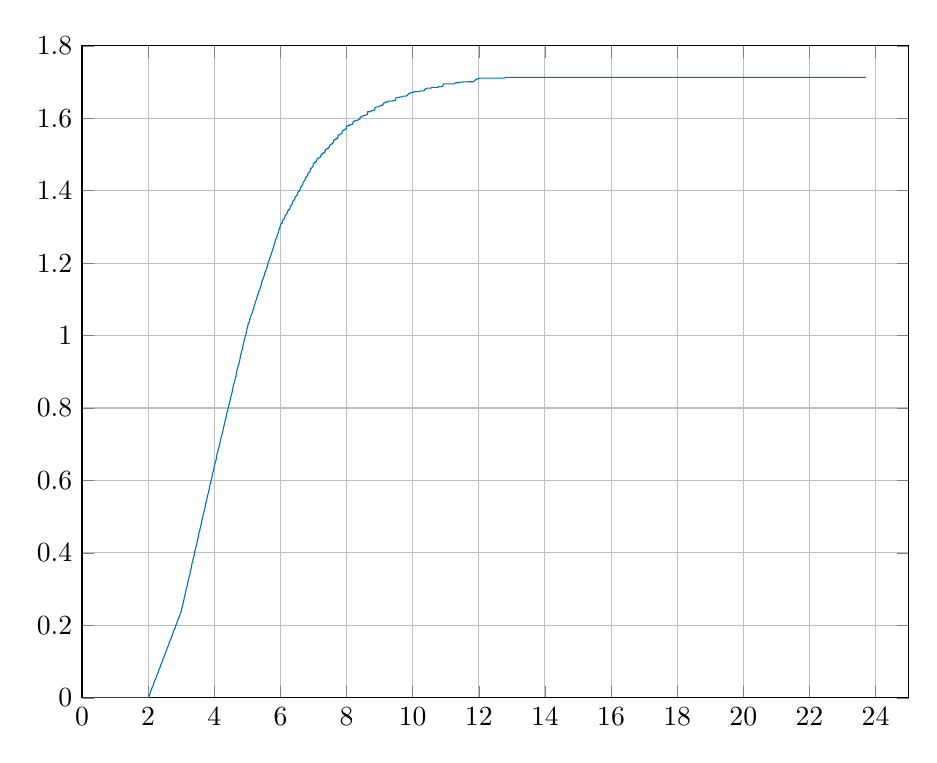
\begin{tikzpicture}

\begin{axis}[%
width=4.133in,
height=3.26in,
at={(0.693in,0.44in)},
scale only axis,
xmin=0,
xmax=25,
xmajorgrids,
ymin=0,
ymax=1.8,
ymajorgrids,
axis background/.style={fill=white}
]
\addplot [color=mycolor1,solid,forget plot]
  table[row sep=crcr]{%
0	0\\
0.0159729680000003	0\\
0.0319338129990008	0\\
0.0502433389999997	0\\
0.0655789880010001	0\\
0.0807258700009994	0\\
0.0960729890000001	0\\
0.112036055	0\\
0.128161949000001	0\\
0.144050576001	0\\
0.160048921	0\\
0.176030784	0\\
0.192037739	0\\
0.208037833001001	0\\
0.224080819	0\\
0.240647512	0\\
0.2566214	0\\
0.271896785	0\\
0.289959384	0\\
0.305120738	0\\
0.320473889001001	0\\
0.336152263	0\\
0.35205965	0\\
0.368188445	0\\
0.384014342	0\\
0.400228368001999	0\\
0.416159189999999	0\\
0.432085597999999	0\\
0.448031429	0\\
0.464044958001001	0\\
0.480174381000001	0\\
0.496318912	0\\
0.512599929	0\\
0.527921844000001	0\\
0.544017256000001	0\\
0.560180254000001	0\\
0.576298661	0\\
0.593196734999999	0\\
0.608588064999999	0\\
0.624195044	0\\
0.640184544	0\\
0.656180279000999	0\\
0.672107728	0\\
0.688044904999001	0\\
0.7040456	0\\
0.727892064000999	0\\
0.736705629000001	0\\
0.751928787	0\\
0.767997738	0\\
0.784059498	0\\
0.800123871999999	0\\
0.816119843	0\\
0.832162914000001	0\\
0.848257537	0\\
0.864159744000001	0\\
0.880177794	0\\
0.896201171	0\\
0.912173548	0\\
0.928106915999999	0\\
0.944051464	0\\
0.960030532	0\\
0.975941729	0\\
0.992198374	0\\
1.008069146001	0\\
1.025285771001	0\\
1.040631098	0\\
1.056244704	0\\
1.07214171	0\\
1.088198629	0\\
1.104168625	0\\
1.120169255	0\\
1.136249120001	0\\
1.152195566001	0\\
1.168239512	0\\
1.184157565	0\\
1.200209472001	0\\
1.216207621	0\\
1.233590443	0\\
1.248644794	0\\
1.264212366999	0\\
1.280020071	0\\
1.296079306	0\\
1.312044006	0\\
1.328083108	0\\
1.343942816001	0\\
1.359878433	0\\
1.375894442	0\\
1.391888523	0\\
1.407872942	0\\
1.423950464	0\\
1.440067251	0\\
1.455965318	0\\
1.47210815	0\\
1.48795017	0\\
1.506062087001	0\\
1.521448853	0\\
1.536945785	0\\
1.552241413001	0\\
1.568209735	0\\
1.584196173001	0\\
1.600056696001	0\\
1.616119856	0\\
1.632294262001	0\\
1.648174861	0\\
1.664222372	0\\
1.680188409	0\\
1.696138361	0\\
1.712164543	0\\
1.729855504	0\\
1.74515857	0\\
1.760145671	0\\
1.775955012001	0\\
1.792227992	0\\
1.808244009	0\\
1.824064932	0\\
1.840171537	0\\
1.856218914	0\\
1.872072134	0\\
1.888187535	0\\
1.90428301	0\\
1.920283515	0\\
1.936059788	0\\
1.952048952	0\\
1.968049527	0\\
1.983992351	0\\
1.999911782	0\\
2.018029829	0.00390129221438598\\
2.033238607	0.00585182266068796\\
2.048407894001	0.00975303774800696\\
2.064055064001	0.014095570578302\\
2.080043822	0.0188810011065946\\
2.096051364001	0.0208316086799635\\
2.112032725	0.0266832316385683\\
2.128172832	0.0305840471434704\\
2.144050098	0.0325345775897724\\
2.160089311001	0.0364352837996979\\
2.176176998	0.0427285818400052\\
2.192200640999	0.0455648886922159\\
2.208059731	0.0494656257684423\\
2.224174314	0.0514161264897504\\
2.240022239	0.0553166465422535\\
2.255994543	0.0611674497306629\\
2.271962354	0.0631175626832478\\
2.287983199	0.0674610249421446\\
2.304122484999	0.0702987082293426\\
2.320042120001	0.0761494014602158\\
2.33619757	0.0800496118162164\\
2.352188944999	0.0819998331601085\\
2.368582841	0.0878499963456331\\
2.384035385001	0.0917500516751693\\
2.39999378	0.0941439733458425\\
2.416054346	0.0989327259255498\\
2.432015367	0.100883033740179\\
2.448095998001	0.106733000360683\\
2.464138544	0.110632865024927\\
2.48003791	0.11258278287818\\
2.495950976	0.116482527798385\\
2.511970052001	0.12277652809755\\
2.528181568	0.125617014288602\\
2.544197863	0.129516603825949\\
2.560149658001	0.131466584490188\\
2.576061837	0.137315913239933\\
2.592281186001	0.141215347275634\\
2.608041285	0.143165093401999\\
2.624130065	0.147509598493732\\
2.640031524999	0.154250612479635\\
2.656034291	0.156200464047403\\
2.672098921	0.160099700262259\\
2.688035757001	0.16204937838985\\
2.704049291999	0.167898179193504\\
2.720130525	0.171797162265079\\
2.736532177	0.174192643313167\\
2.752030173	0.178984950844335\\
2.768011472	0.184833560932873\\
2.784275828	0.186783169286806\\
2.800135006	0.190681980128135\\
2.816238265999	0.192631465604442\\
2.832184658001	0.198479412997117\\
2.848202079	0.202824908223995\\
2.864174325	0.205669199527163\\
2.880158501	0.209567910477965\\
2.896135857	0.215415775421132\\
2.912019936	0.217365128709221\\
2.928155133	0.221263366583194\\
2.944247065	0.223212654917376\\
2.960164733	0.229507634685106\\
2.976062095001	0.234302481959576\\
2.992004368	0.236251692156931\\
3.007953966	0.242099088101009\\
3.025479115	0.249875298373959\\
3.040719209	0.2537663654061\\
3.056066309	0.260579700632209\\
3.072081187	0.266855198349112\\
3.08801676	0.273600115376734\\
3.104056173	0.281376389015973\\
3.120037385	0.285267570808725\\
3.136031721	0.293050727716208\\
3.152059533001	0.301327099352919\\
3.168061456	0.303753513711781\\
3.18403932	0.311978549715949\\
3.200030544	0.318705653342465\\
3.216225229001	0.324552149748091\\
3.232017183	0.332328511955244\\
3.247994805	0.336219599137683\\
3.266081787	0.343029827782619\\
3.281550773	0.352754537414753\\
3.296781978	0.355153179653011\\
3.312188638	0.363830385121104\\
3.328071805	0.371607058018644\\
3.344070069999	0.375504223890061\\
3.360182644001	0.383779443327977\\
3.376186768	0.388146450355597\\
3.392219595999	0.393980030132013\\
3.408185102001	0.404155521736048\\
3.424089102999	0.407006380332663\\
3.440192942	0.414782888288449\\
3.456147103	0.419172049667341\\
3.476276741001	0.426954386349302\\
3.488050213999	0.435205790955126\\
3.504212498001	0.439096900658528\\
3.51998871	0.446285474360122\\
3.535912234	0.4560104748117\\
3.552115598	0.457958821585639\\
3.568058533001	0.466232666624352\\
3.584035722	0.47059825264762\\
3.600212326	0.478380072738835\\
3.616187404	0.486156213204328\\
3.632180788	0.49140482592041\\
3.648263174	0.4972383068124\\
3.66417606	0.507459730148828\\
3.68017186	0.509407727877582\\
3.696179336	0.517658056638797\\
3.712171001	0.521549123981304\\
3.729286257001	0.529330444499592\\
3.744296627	0.538466369220232\\
3.759949635	0.540910427497364\\
3.776025644	0.548686947360285\\
3.79243516	0.558884531359128\\
3.808061738001	0.560832483293686\\
3.824233371	0.568608675399514\\
3.840180605	0.572499505309264\\
3.856178189	0.581642519753468\\
3.872188361	0.589914413386395\\
3.888158657	0.591862087237313\\
3.904183363001	0.600111213904867\\
3.920177844	0.605949813443569\\
3.936154620001	0.611782659727193\\
3.952159566001	0.620013460193598\\
3.96817319	0.625309106293798\\
3.985026427001	0.631141985916024\\
3.999962639001	0.640866108766864\\
4.015934122	0.645229136784081\\
4.032031366	0.651062181289126\\
4.048092037	0.654953409491215\\
4.064263144	0.661280452258581\\
4.080187005001	0.672369833030241\\
4.096047758	0.676261042638489\\
4.112093712	0.682565494068476\\
4.128037253	0.688394808579014\\
4.144149446	0.692289909094449\\
4.160372495001	0.69811950559455\\
4.176183717	0.706399299531388\\
4.192207374	0.71314243960879\\
4.208212946	0.719427206699914\\
4.227966453	0.725736571880037\\
4.24084297	0.729622565683421\\
4.255903446001	0.735461519465477\\
4.273986179	0.743735156058037\\
4.289203981	0.749565070499579\\
4.304420253	0.755858768763402\\
4.320216633001	0.76112492578141\\
4.33637252	0.768902573594352\\
4.352049437	0.772794294632193\\
4.368082681	0.779119773693457\\
4.384032913	0.788845054384441\\
4.40004105	0.790792689379396\\
4.416015085	0.798570522683946\\
4.432031952	0.804296433297919\\
4.448049737	0.810130165007727\\
4.464039708001	0.815960769175224\\
4.482074767001	0.822294640069407\\
4.497084121	0.830072618756126\\
4.512021607	0.833964585412403\\
4.527972196	0.839798494743978\\
4.543941799	0.846552322511933\\
4.559896918001	0.85330211231576\\
4.576152891	0.861574177396703\\
4.592043393	0.867405090810269\\
4.608124328	0.871300122591168\\
4.62405134	0.877131281273966\\
4.64013372	0.883438433589979\\
4.656121552	0.887325130423459\\
4.672036949	0.898906252850851\\
4.688038486	0.904745745765923\\
4.704034807	0.908632528080171\\
4.720143939001	0.916411365503735\\
4.735906383	0.91835903154178\\
4.754073761	0.926604896193301\\
4.770136309	0.932444747198223\\
4.785571488001	0.939678286619449\\
4.800983084	0.947912257761491\\
4.816422589	0.951804714055424\\
4.832274072	0.957639072743047\\
4.848198164	0.961531574306512\\
4.864177461	0.969779856346548\\
4.880195099001	0.978047605912073\\
4.896159187001	0.982394678775878\\
4.912127449999	0.989139543815664\\
4.928038828	0.994971637058266\\
4.944039503	1.00081169133252\\
4.96004975	1.00469890016451\\
4.976112186001	1.01295196900468\\
4.991999217	1.01927426590228\\
5.010145583	1.02510670639984\\
5.025292076	1.03231189175854\\
5.040580172001	1.03425155072189\\
5.056208028	1.03814433225611\\
5.072187366	1.04397902300035\\
5.08828907	1.04881659051279\\
5.104217176	1.05270937204701\\
5.120175716	1.05854406279125\\
5.136203864	1.06048920933051\\
5.152158590001	1.06437650328881\\
5.168132064001	1.07021668160898\\
5.184163715001	1.07215634057232\\
5.200209267	1.07894154307972\\
5.216061066001	1.08478172139988\\
5.232149069001	1.08808638740176\\
5.248044621001	1.09392672454771\\
5.264006537	1.09781385968022\\
5.279895171	1.09975900621949\\
5.296146479	1.10754133195869\\
5.31230402	1.11237889947113\\
5.328191812001	1.11432404601039\\
5.344121886	1.12210637174959\\
5.360203615	1.12405151828885\\
5.376180657	1.1259911772522\\
5.392042773	1.13377899056731\\
5.408452711	1.13571864953066\\
5.424190481	1.14386885907659\\
5.440145232999	1.14970903739675\\
5.456187783001	1.1516486963601\\
5.472121918001	1.15554147789432\\
5.489033858	1.16137616863856\\
5.504020137001	1.16332131517782\\
5.51995627	1.16915375567539\\
5.538209002	1.17594120842946\\
5.553528814001	1.17788635496873\\
5.569029943	1.18177364892703\\
5.584494414999	1.18761382724719\\
5.600321371	1.18955348621053\\
5.616220803	1.19584126896454\\
5.632055603	1.2025911120668\\
5.648776329	1.20501833959549\\
5.664058871	1.20937631457419\\
5.680034106001	1.21521100531844\\
5.6960119	1.2171561518577\\
5.712358840001	1.221043445816\\
5.730011721	1.22882328309951\\
5.74412545	1.23076842963877\\
5.760327879	1.23514329216242\\
5.777762916	1.24144866392706\\
5.793189452	1.24338832289041\\
5.80869458	1.25117613620553\\
5.824150672	1.25448080220741\\
5.840040631	1.25836560771002\\
5.856046103	1.26615342102513\\
5.872099302	1.26858064855383\\
5.890645178	1.27099098853757\\
5.906185481	1.27877331427677\\
5.921747453	1.28071846081604\\
5.937107878	1.28460326631864\\
5.952485733	1.29238559205784\\
5.968051538	1.29433073859711\\
5.983990609001	1.29870560112075\\
6.000069857001	1.3050109728854\\
6.016292089	1.30740597410519\\
6.032071739	1.31026061307276\\
6.048296157	1.31026061307276\\
6.064169956	1.31804293881196\\
6.080015525	1.31998816651317\\
6.096201921	1.31998806805126\\
6.112070735	1.3219277270146\\
6.128040774	1.3238730358185\\
6.144189224001	1.3321429054345\\
6.160037374	1.3321429054345\\
6.176109328001	1.33408829528184\\
6.192160399	1.33649183857425\\
6.208192397	1.33843947356921\\
6.224336588	1.34427997618162\\
6.23994943	1.34621941809181\\
6.258101535	1.34816496984823\\
6.273467481001	1.34816496984823\\
6.289028978	1.35205212015706\\
6.304498325	1.35789278456002\\
6.320191393	1.35838035312537\\
6.336107232	1.36031994172439\\
6.352148139001	1.36317599976008\\
6.368181719	1.36947332896723\\
6.384218266	1.37187546778784\\
6.400195473	1.3738212619634\\
6.416187594	1.3738212619634\\
6.432171256	1.37576092092674\\
6.448150683	1.38354919880415\\
6.464158300001	1.38354919880415\\
6.481555761	1.3854888577675\\
6.496534606001	1.38743462241306\\
6.511933971	1.38792219097841\\
6.527970923	1.39570451671761\\
6.544149455	1.39765043472935\\
6.560053862	1.39765043472935\\
6.575997260999	1.40005155186888\\
6.594282805001	1.40394491840954\\
6.609756506	1.40783995019044\\
6.62505428	1.41172572572503\\
6.640139797	1.41172549369595\\
6.656078337	1.41366515265929\\
6.672082726	1.41755898467621\\
6.688033744	1.42330643239982\\
6.704035477	1.42524609136316\\
6.720083369	1.42719236877656\\
6.736369878	1.42719236877656\\
6.752016216	1.43302713093474\\
6.767966866	1.43738106432384\\
6.784039221	1.43738106432384\\
6.80005026	1.43932036829557\\
6.816245626	1.44126680631399\\
6.83225245	1.44710947308984\\
6.848169351	1.44904884905974\\
6.864157373001	1.45099536729173\\
6.880229676	1.45148293585708\\
6.896051046	1.45342238370657\\
6.912286864	1.46121164886868\\
6.928233462001	1.46121164886868\\
6.944250970001	1.46315116847918\\
6.960184499	1.46509784696042\\
6.978704118	1.46555658750874\\
6.993743258	1.47333850577104\\
7.009115177001	1.4757406065444\\
7.023913989999	1.4761956088952\\
7.040149615	1.47858959432279\\
7.056045032	1.47858965304494\\
7.072053345	1.48053649153824\\
7.088034687	1.48102372156181\\
7.104086914	1.48686583538682\\
7.120034695	1.48880566442552\\
7.136046529999	1.48880566442552\\
7.152039604	1.49075217755132\\
7.168012226	1.49075217755132\\
7.183988957	1.49075217755132\\
7.199999756	1.49269175388554\\
7.215996848	1.49269175388554\\
7.232039903	1.50048149872799\\
7.247993297001	1.5004812234956\\
7.263971508	1.5004812234956\\
7.279918161	1.50287800894438\\
7.295932783001	1.50482469874192\\
7.311912627	1.50482469874192\\
7.327922337001	1.50482469874192\\
7.343908164999	1.50676446641708\\
7.359920481001	1.51260713319293\\
7.375961985	1.51455445029903\\
7.392040226	1.51503964876062\\
7.408335884	1.51503897130249\\
7.424076336	1.51697930914903\\
7.440035221	1.51697930914903\\
7.456165529999	1.51892617481174\\
7.471912	1.51892617481174\\
7.489031093	1.52476884158759\\
7.504691260001	1.52670879979814\\
7.520037116	1.52670879979814\\
7.536157297	1.52865635540987\\
7.552317769001	1.52911129499882\\
7.5681815	1.52956629734962\\
7.583995232001	1.53196155123346\\
7.599960107	1.53241553760142\\
7.615939895	1.54020591869613\\
7.631991546	1.54020591869613\\
7.647936524001	1.54020543464219\\
7.663933282	1.54214606417248\\
7.679933324	1.54214606417248\\
7.695940539999	1.5440938577559\\
7.711883441001	1.54457621613046\\
7.730128201	1.54457621613046\\
7.745170319999	1.55235972743286\\
7.760205227	1.55235898553464\\
7.776058318	1.5543069374692\\
7.79200196	1.5543069374692\\
7.808074282	1.55624726940039\\
7.824198801	1.55624726940039\\
7.840164805	1.55819530042151\\
7.856042889	1.55819476429106\\
7.872023193	1.56403743106692\\
7.888020640999	1.56597852813536\\
7.904039899001	1.56597805768543\\
7.920161177	1.56792624670165\\
7.936024056	1.56837852930918\\
7.951991581	1.56837777929678\\
7.96799389	1.57031904443085\\
7.986729956	1.57031904443085\\
8.000056338999	1.57810948608401\\
8.015943756	1.57859016831989\\
8.031934898	1.57859016831989\\
8.047952063	1.57859016831989\\
8.063983156001	1.5805311404665\\
8.0801402	1.5805311404665\\
8.096036655	1.5805311404665\\
8.112039404999	1.58247910094094\\
8.128030584	1.58247910094094\\
8.144195101	1.58247910094094\\
8.160147031	1.58293404752998\\
8.176041416	1.58338904988078\\
8.19204389	1.5872782060482\\
8.208028424	1.59117299588456\\
8.224041097	1.59162765831586\\
8.239959869	1.59162765831586\\
8.258049312	1.593575674335\\
8.272963982999	1.593575674335\\
8.288363278	1.593575674335\\
8.304027551	1.59357533415318\\
8.320189389001	1.59357533415318\\
8.336194046	1.59551718565407\\
8.352220099001	1.59551718565407\\
8.368166557001	1.59551691957533\\
8.384198123	1.59746526634927\\
8.400185192001	1.59746526634927\\
8.415990348	1.60330765756023\\
8.432110029999	1.60330765756023\\
8.448043814	1.60375926009397\\
8.464001041	1.60570107695665\\
8.480098389001	1.60570107695665\\
8.49595773	1.60570107695665\\
8.511939935	1.60764921254603\\
8.528033467	1.60764921254603\\
8.54418576	1.60812661844373\\
8.560191192	1.60812605873133\\
8.576160892001	1.60812605873133\\
8.592101862	1.61006832729115\\
8.608067093	1.61006784125322\\
8.624074227001	1.61006784125322\\
8.640265354001	1.61785885480302\\
8.656172954	1.61785885480302\\
8.672179022	1.61785835914612\\
8.688210989	1.61785835914612\\
8.704295103	1.61785835914612\\
8.720142331	1.61980037195549\\
8.736064104	1.61980037195549\\
8.752008265999	1.61980037195549\\
8.769340121	1.62174828689143\\
8.784556934	1.62174828689143\\
8.80006042	1.62174828689143\\
8.815977016	1.62174784537533\\
8.832184876	1.62174784537533\\
8.848172476	1.62369540098705\\
8.864250362	1.62953282803506\\
8.880142687	1.62953282803506\\
8.896181308	1.631481174809\\
8.91214505	1.63148079681599\\
8.927992014001	1.63148079681599\\
8.944189659	1.63148079681599\\
8.960184738001	1.63148040908575\\
8.976068232001	1.63148040908575\\
8.992207513	1.63342334186315\\
9.008028939	1.63387494439689\\
9.025214451	1.6338746296903\\
9.041485206	1.63582297646424\\
9.056331349001	1.63582297646424\\
9.07187652	1.63582265196125\\
9.087947407	1.63582265196125\\
9.10416093	1.63777020757298\\
9.120098493002	1.64166498443772\\
9.13608466	1.64213832158802\\
9.152058394001	1.64259366384447\\
9.16804151	1.64304798294325\\
9.184031206	1.64499124640907\\
9.200034412	1.64499124640907\\
9.215962844	1.6449906358704\\
9.234431173	1.6449906358704\\
9.249515239001	1.6449906358704\\
9.264520604	1.6469383622357\\
9.280567420001	1.64739302466699\\
9.296168811001	1.64739302466699\\
9.312077217	1.64739302466699\\
9.328065991	1.64739239438841\\
9.34392414	1.64739239438841\\
9.36000381	1.64739239438841\\
9.376067872	1.64739175423991\\
9.392070663	1.64739175423991\\
9.408038319	1.64933534744704\\
9.424044376	1.64933477971596\\
9.440070344	1.64933477971596\\
9.456039017	1.64933477971596\\
9.472044373001	1.64933420205578\\
9.48824116	1.65517758061062\\
9.50395095	1.65712521560557\\
9.519983256	1.65712462801633\\
9.536050452	1.65712462801633\\
9.552020304	1.65712462801633\\
9.567995572	1.65712403049802\\
9.58418366	1.65712403049802\\
9.600172355	1.65712403049802\\
9.616129588001	1.65906795249918\\
9.632222733	1.65906742710231\\
9.648174227	1.65906742710231\\
9.664222661001	1.65906742710231\\
9.680047272	1.65906689171721\\
9.696154268	1.65906689171721\\
9.712168199001	1.66101523849115\\
9.731033397999	1.66101469311783\\
9.743936703001	1.66101469311783\\
9.760006129	1.66101469311783\\
9.775963502	1.66101413775631\\
9.792140605	1.66101413775631\\
9.808180946001	1.66101413775631\\
9.824053092	1.66295790406792\\
9.840107649	1.66295790406792\\
9.856150069	1.66490545967965\\
9.872158354001	1.6668524422653\\
9.888461708	1.66880007726025\\
9.904198043001	1.66880007726025\\
9.920116953	1.66879957362935\\
9.936171452	1.67074792040329\\
9.952166794	1.67119952293703\\
9.968483626	1.67119952293703\\
9.984090613	1.67119900925876\\
9.999948186	1.67119900925876\\
10.015970784	1.67166657880028\\
10.032010647999	1.67166657880028\\
10.048125989	1.67361115554699\\
10.064043275	1.67361115554699\\
10.080173414	1.67361115554699\\
10.096143449999	1.67361115554699\\
10.112138638	1.67361115554699\\
10.128084835	1.67361115554699\\
10.144064844	1.67361115554699\\
10.160035381	1.67361115554699\\
10.176035495001	1.67361115554699\\
10.191997844	1.67361115554699\\
10.208004293001	1.67361115554699\\
10.224326487	1.67555950232093\\
10.239945812999	1.67555950232093\\
10.255898808	1.67555950232093\\
10.273927475	1.67555950232093\\
10.289326178	1.67555950232093\\
10.304785521001	1.67555950232093\\
10.320255687001	1.67555950232093\\
10.336069506999	1.67555950232093\\
10.352138027	1.67750705793266\\
10.368045857	1.67945453410183\\
10.384180461	1.68140216909679\\
10.400172126	1.68140216909679\\
10.416183511	1.68140216909679\\
10.432161846	1.68334674584349\\
10.448173581	1.68334674584349\\
10.464140005	1.68334674584349\\
10.482287107	1.68334674584349\\
10.497495508	1.68334674584349\\
10.512497438	1.68334674584349\\
10.527972957	1.68334674584349\\
10.544142342	1.68334674584349\\
10.560031424	1.68334674584349\\
10.576141517	1.68529509261743\\
10.592037599001	1.68529509261743\\
10.609671774001	1.68529509261743\\
10.625008131	1.68529509261743\\
10.640402804	1.68529509261743\\
10.656164118	1.68529509261743\\
10.672190235	1.68529509261743\\
10.688186951999	1.68529509261743\\
10.704059006	1.68529509261743\\
10.720090631999	1.68529509261743\\
10.737150978	1.68529509261743\\
10.752113685	1.68529509261743\\
10.768130469	1.68529509261743\\
10.784190159	1.68723966936414\\
10.800178982	1.68723966936414\\
10.816039807	1.68723966936414\\
10.832205776	1.68723966936414\\
10.848187659	1.68723966936414\\
10.864180918	1.68723966936414\\
10.880154442	1.68723966936414\\
10.896027057	1.68723966936414\\
10.912025432	1.69113565113304\\
10.928178964	1.69308320674476\\
10.944048247	1.69503068291394\\
10.960043155	1.69503068291394\\
10.976052119	1.69503068291394\\
10.991908186001	1.69503068291394\\
11.009988561001	1.69503068291394\\
11.024827267	1.69503006451852\\
11.040053674	1.69503006451852\\
11.056133254	1.6950297238076\\
11.071945234	1.6950290951729\\
11.088052543001	1.6950290951729\\
11.104075544	1.69502874419207\\
11.120025890999	1.69502810531811\\
11.136094986001	1.69502810531811\\
11.152140268	1.6950277440674\\
11.168063062	1.6950277440674\\
11.184063553	1.6950270949542\\
11.200038209	1.6950267234336\\
11.216081871999	1.6950267234336\\
11.233141331	1.69502606408117\\
11.248102499	1.69502568229071\\
11.264532299	1.69548102454715\\
11.28046865	1.69742542027359\\
11.296037792	1.69742502821327\\
11.312032419	1.69788003056407\\
11.32807544	1.69787943195446\\
11.344099539	1.69787943195446\\
11.360080856	1.69787902962429\\
11.376117838	1.69787842071627\\
11.392005031999	1.69787842071627\\
11.407996948001	1.69787800811626\\
11.423986117	1.69982636434047\\
11.439995112	1.69982636434047\\
11.456184379	1.69982601978559\\
11.472182914999	1.6998253902808\\
11.48874183	1.6998253902808\\
11.504025692	1.69982503539674\\
11.52000991	1.69982503539674\\
11.537708722	1.70027905802488\\
11.552966781	1.70027869281165\\
11.568401765	1.70027869281165\\
11.584237572	1.70027804271017\\
11.600469782	1.70027766716778\\
11.616164284	1.70027766716778\\
11.63195769	1.70027700676798\\
11.648231958001	1.70027662089645\\
11.664316586	1.70027662089645\\
11.680126991001	1.70072313091484\\
11.696190902	1.70072313091484\\
11.712149256999	1.70072239447874\\
11.728108416	1.70072171348236\\
11.744023636	1.70072171348236\\
11.760030853	1.70072096670353\\
11.776023827	1.7007202754089\\
11.792174617	1.7007202754089\\
11.808222775	1.70071951828735\\
11.824165219	1.70071881669448\\
11.840304378	1.70071881669448\\
11.856361090001	1.7026656842252\\
11.872149601	1.70461323983693\\
11.888234397	1.70461252794584\\
11.904271685	1.70655922630812\\
11.920044645	1.70655922630812\\
11.936016074	1.70850462069008\\
11.952178972001	1.70850383254054\\
11.968195844	1.70896495106233\\
11.986078922001	1.70896395935717\\
12.001339043	1.70896316086501\\
12.016265316001	1.71091307215598\\
12.031931226	1.71091207007935\\
12.048009648	1.71091207007935\\
12.064169068	1.71091133884693\\
12.080301652	1.71091032639887\\
12.096156818	1.71091032639887\\
12.112174407	1.71090958476448\\
12.128041014001	1.71090958476448\\
12.144153206999	1.710908561945\\
12.160394543	1.71090780990867\\
12.17624791	1.71090780990867\\
12.192154627	1.71090677671782\\
12.208275019001	1.71090601427956\\
12.224158870001	1.71090601427956\\
12.241515324	1.71090497071737\\
12.256561543	1.71090419787721\\
12.271960162	1.71090419787721\\
12.288213384	1.7109031439437\\
12.304176435	1.71090236070167\\
12.320179792	1.71090236070167\\
12.336184627	1.71090129639688\\
12.352190143	1.71090129639688\\
12.368177694001	1.71090050275299\\
12.384239172001	1.71089942807696\\
12.400161661	1.71089942807696\\
12.416221645	1.71089862403124\\
12.432234704	1.71089753898399\\
12.448051949	1.71089753898399\\
12.464163681	1.71089672453647\\
12.484072635	1.71089672453647\\
12.496366747	1.71089562911804\\
12.512473144001	1.71089480426874\\
12.527935561001	1.71089480426874\\
12.545973069999	1.71089369847916\\
12.561401297001	1.71089286322811\\
12.57681111	1.71089286322811\\
12.592598188	1.71089174706741\\
12.6080558	1.71089090141463\\
12.624212893	1.71089090141463\\
12.640194465	1.71088977488285\\
12.656215081	1.71088891882837\\
12.672189156001	1.71088891882837\\
12.688070962001	1.71088778192554\\
12.704157442	1.71088778192554\\
12.72012356	1.71088691546938\\
12.738214099001	1.71088576819555\\
12.752076411	1.71088576819555\\
12.768067005	1.71088489133773\\
12.783932413001	1.71088373369292\\
12.799947800001	1.71283120986209\\
12.816190205	1.71283032260266\\
12.83222166	1.71283032260266\\
12.848154417	1.71282923402946\\
12.864182625	1.71282833636842\\
12.880251475	1.71282833636842\\
12.896192315	1.71282723736499\\
12.912158292	1.71282632930239\\
12.928052942	1.71282632930239\\
12.944049974001	1.71282521986875\\
12.96004431	1.71282430140461\\
12.976027566001	1.71282430140461\\
12.992043908001	1.71282318154081\\
13.007992924	1.71282318154081\\
13.023989373	1.71282318154081\\
13.040009656	1.71282205124688\\
13.056184661999	1.71282205124688\\
13.072210540001	1.71282205124688\\
13.088196963999	1.71282091052286\\
13.104192456	1.71282091052286\\
13.120185407	1.71282091052286\\
13.136173441001	1.71282091052286\\
13.15217505	1.71281975936877\\
13.168176858	1.71281975936877\\
13.184172196001	1.71281975936877\\
13.200043107999	1.71281859778466\\
13.216181846	1.71281859778466\\
13.235255373	1.71281859778466\\
13.247900283001	1.71281742577055\\
13.263955441001	1.71281742577055\\
13.279950710002	1.71281742577055\\
13.296181447	1.71281624332649\\
13.312222072	1.71281624332649\\
13.328359680001	1.71281624332649\\
13.344152947999	1.71281505045251\\
13.360052109001	1.71281505045251\\
13.376032123001	1.71281505045251\\
13.392034982999	1.71281384714865\\
13.408367084	1.71281384714865\\
13.424261294	1.71281384714865\\
13.440187621	1.71281263341494\\
13.456383188	1.71281263341494\\
13.47228053	1.71281263341494\\
13.489396531001	1.71281263341494\\
13.505576413001	1.71281140925142\\
13.520455183	1.71281140925142\\
13.536028725	1.71281140925142\\
13.552175215999	1.71281017465813\\
13.568304359	1.71281017465813\\
13.584071399001	1.71281017465813\\
13.600187080001	1.7128089296351\\
13.616186798	1.7128089296351\\
13.632163088001	1.7128089296351\\
13.648176859001	1.71280767418238\\
13.664333242	1.71280767418238\\
13.680238236001	1.71280767418238\\
13.69617643	1.7128064083\\
13.712174966	1.7128064083\\
13.728322499	1.7128064083\\
13.745056606	1.71280513198799\\
13.760624085002	1.71280513198799\\
13.777398955	1.71280513198799\\
13.792420245	1.71280513198799\\
13.808225072999	1.71280384524641\\
13.824291929	1.71280384524641\\
13.840047925	1.71280384524641\\
13.856041269	1.71280254807529\\
13.872033305	1.71280254807529\\
13.888039789	1.71280254807529\\
13.904040279	1.71280124047466\\
13.920015086	1.71280124047466\\
13.936008564001	1.71280124047466\\
13.952116689	1.71279992244457\\
13.968042951	1.71279992244457\\
13.984121703	1.71279992244457\\
13.99992643	1.71279859398505\\
14.017126861001	1.71279859398505\\
14.032133811001	1.71279859398505\\
14.047897722001	1.71279859398505\\
14.063960238	1.71279859398505\\
14.080229802001	1.71279859398505\\
14.096056253	1.71279859398505\\
14.112028154	1.71279859398505\\
14.128039433	1.71279859398505\\
14.144070317	1.71279859398505\\
14.160044112	1.71279859398505\\
14.176016994	1.71279859398505\\
14.192043995001	1.71279859398505\\
14.208043879	1.71279859398505\\
14.22404493	1.71279859398505\\
14.240166553	1.71279859398505\\
14.256026214	1.71279859398505\\
14.271945394001	1.71279859398505\\
14.287959192	1.71279859398505\\
14.304090668999	1.71279859398505\\
14.320067074	1.71279859398505\\
14.336073658001	1.71279859398505\\
14.352013356	1.71279859398505\\
14.367991545001	1.71279859398505\\
14.383992291	1.71279859398505\\
14.399990164999	1.71279859398505\\
14.416042852999	1.71279859398505\\
14.432047052	1.71279859398505\\
14.448024164	1.71279859398505\\
14.46404061	1.71279859398505\\
14.480043651	1.71279859398505\\
14.495906952	1.71279859398505\\
14.512016565	1.71279859398505\\
14.527977513	1.71279859398505\\
14.543893447	1.71279859398505\\
14.560011688	1.71279859398505\\
14.576205191001	1.71279859398505\\
14.592175288	1.71279859398505\\
14.608232677001	1.71279859398505\\
14.62421894	1.71279859398505\\
14.640370557001	1.71279859398505\\
14.656199108	1.71279859398505\\
14.672188784	1.71279859398505\\
14.688245491001	1.71279859398505\\
14.704174324	1.71279859398505\\
14.720193997	1.71279859398505\\
14.736122568	1.71279859398505\\
14.752019796	1.71279859398505\\
14.768034377	1.71279859398505\\
14.783915691001	1.71279859398505\\
14.800160476	1.71279859398505\\
14.816220406001	1.71279859398505\\
14.832290218	1.71279859398505\\
14.848169018	1.71279859398505\\
14.864182899	1.71279859398505\\
14.880185182	1.71279859398505\\
14.896162024	1.71279859398505\\
14.912160664999	1.71279859398505\\
14.928055661001	1.71279859398505\\
14.944023552	1.71279859398505\\
14.960032272	1.71279859398505\\
14.976051008	1.71279859398505\\
14.991939251	1.71279859398505\\
15.007951868	1.71279859398505\\
15.025100583	1.71279859398505\\
15.040487778001	1.71279859398505\\
15.056136907	1.71279859398505\\
15.072147746001	1.71279859398505\\
15.088283483	1.71279859398505\\
15.104189654	1.71279859398505\\
15.120151617	1.71279859398505\\
15.136156261	1.71279859398505\\
15.152161788	1.71279859398505\\
15.168331492	1.71279859398505\\
15.18419665	1.71279859398505\\
15.200158889001	1.71279859398505\\
15.216178337001	1.71279859398505\\
15.235760084	1.71279859398505\\
15.24795061	1.71279859398505\\
15.26604889	1.71279859398505\\
15.281086479001	1.71279859398505\\
15.296510965	1.71279859398505\\
15.312066807	1.71279859398505\\
15.328064622	1.71279859398505\\
15.344075187	1.71279859398505\\
15.360040373	1.71279859398505\\
15.376062557	1.71279859398505\\
15.392026772	1.71279859398505\\
15.408005755001	1.71279859398505\\
15.424035009	1.71279859398505\\
15.440295293	1.71279859398505\\
15.456192599001	1.71279859398505\\
15.472213882001	1.71279859398505\\
15.488088749	1.71279859398505\\
15.505285696001	1.71279859398505\\
15.520638631	1.71279859398505\\
15.536150358	1.71279859398505\\
15.552179693	1.71279859398505\\
15.568052476	1.71279859398505\\
15.584162093	1.71279859398505\\
15.600525891	1.71279859398505\\
15.61614409	1.71279859398505\\
15.632177099001	1.71279859398505\\
15.648173389	1.71279859398505\\
15.664433979001	1.71279859398505\\
15.680206247	1.71279859398505\\
15.696167102	1.71279859398505\\
15.712184941001	1.71279859398505\\
15.728164559	1.71279859398505\\
15.746060789	1.71279859398505\\
15.7610405	1.71279859398505\\
15.776132782	1.71279859398505\\
15.791981589	1.71279859398505\\
15.808024793001	1.71279859398505\\
15.824217428	1.71279859398505\\
15.840222097001	1.71279859398505\\
15.856151631999	1.71279859398505\\
15.872176107	1.71279859398505\\
15.8881031	1.71279859398505\\
15.904153474001	1.71279859398505\\
15.920150485	1.71279859398505\\
15.936174734	1.71279859398505\\
15.952191712001	1.71279859398505\\
15.96817134	1.71279859398505\\
15.986342277	1.71279859398505\\
16.000431818	1.71279859398505\\
16.015879863001	1.71279859398505\\
16.033919727	1.71279859398505\\
16.049118385999	1.71279859398505\\
16.064720729	1.71279859398505\\
16.080212221	1.71279859398505\\
16.096170581	1.71279859398505\\
16.112176538	1.71279859398505\\
16.128148333	1.71279859398505\\
16.144161181	1.71279859398505\\
16.160160078	1.71279859398505\\
16.176173753	1.71279859398505\\
16.19216401	1.71279859398505\\
16.20817549	1.71279859398505\\
16.224368075	1.71279859398505\\
16.240903036	1.71279859398505\\
16.255994651002	1.71279859398505\\
16.27189487	1.71279859398505\\
16.289916779001	1.71279859398505\\
16.305228449	1.71279859398505\\
16.320749357999	1.71279859398505\\
16.336394433	1.71279859398505\\
16.352166395	1.71279859398505\\
16.368200777	1.71279859398505\\
16.384063846	1.71279859398505\\
16.400134636	1.71279859398505\\
16.416039394001	1.71279859398505\\
16.431980224001	1.71279859398505\\
16.44803402	1.71279859398505\\
16.464177403	1.71279859398505\\
16.480459587001	1.71279859398505\\
16.495958129	1.71279859398505\\
16.511991442	1.71279859398505\\
16.52851023	1.71279859398505\\
16.544005182	1.71279859398505\\
16.560179723	1.71279859398505\\
16.576163449999	1.71279859398505\\
16.592148836	1.71279859398505\\
16.608078581	1.71279859398505\\
16.624182956	1.71279859398505\\
16.640207210002	1.71279859398505\\
16.65638301	1.71279859398505\\
16.672044851	1.71279859398505\\
16.688027069	1.71279859398505\\
16.704143565	1.71279859398505\\
16.720185526002	1.71279859398505\\
16.739536867	1.71279859398505\\
16.753102627	1.71279859398505\\
16.769114227	1.71279859398505\\
16.784041905	1.71279859398505\\
16.799949648	1.71279859398505\\
16.815950317	1.71279859398505\\
16.832178959	1.71279859398505\\
16.848212866	1.71279859398505\\
16.864178903001	1.71279859398505\\
16.880163346	1.71279859398505\\
16.896045458001	1.71279859398505\\
16.912033991	1.71279859398505\\
16.928041768	1.71279859398505\\
16.944052792	1.71279859398505\\
16.960036499	1.71279859398505\\
16.976031968	1.71279859398505\\
16.992044071001	1.71279859398505\\
17.008003958	1.71279859398505\\
17.025150875	1.71279859398505\\
17.040755601	1.71279859398505\\
17.056133197	1.71279859398505\\
17.07215813	1.71279859398505\\
17.088041337	1.71279859398505\\
17.104154999	1.71279859398505\\
17.120084523	1.71279859398505\\
17.136036148	1.71279859398505\\
17.152175628	1.71279859398505\\
17.168186196	1.71279859398505\\
17.184187217	1.71279859398505\\
17.200181307001	1.71279859398505\\
17.216202745	1.71279859398505\\
17.232165249	1.71279859398505\\
17.249706369	1.71279859398505\\
17.265727972	1.71279859398505\\
17.281865172001	1.71279859398505\\
17.295915479	1.71279859398505\\
17.312064887001	1.71279859398505\\
17.328179245001	1.71279859398505\\
17.344039488001	1.71279859398505\\
17.360054145	1.71279859398505\\
17.376043880001	1.71279859398505\\
17.392019944999	1.71279859398505\\
17.410266348	1.71279859398505\\
17.425592079	1.71279859398505\\
17.44109835	1.71279859398505\\
17.456378844	1.71279859398505\\
17.472081819999	1.71279859398505\\
17.488815617	1.71279859398505\\
17.504757717	1.71279859398505\\
17.52061691	1.71279859398505\\
17.537280781001	1.71279859398505\\
17.552285132001	1.71279859398505\\
17.568119043	1.71279859398505\\
17.584010657	1.71279859398505\\
17.600143397	1.71279859398505\\
17.616186289	1.71279859398505\\
17.632153097	1.71279859398505\\
17.648151588	1.71279859398505\\
17.664229669	1.71279859398505\\
17.680101517	1.71279859398505\\
17.696182715	1.71279859398505\\
17.712264454	1.71279859398505\\
17.728075907	1.71279859398505\\
17.743904977001	1.71279859398505\\
17.760042430999	1.71279859398505\\
17.775958382001	1.71279859398505\\
17.791922197	1.71279859398505\\
17.807940616	1.71279859398505\\
17.825992071	1.71279859398505\\
17.841296685	1.71279859398505\\
17.856793845	1.71279859398505\\
17.872182241	1.71279859398505\\
17.88822275	1.71279859398505\\
17.90418567	1.71279859398505\\
17.920152333	1.71279859398505\\
17.936261499	1.71279859398505\\
17.952190537	1.71279859398505\\
17.96807957	1.71279859398505\\
17.984555232	1.71279859398505\\
18.00182841	1.71279859398505\\
18.017758463	1.71279859398505\\
18.033180591	1.71279859398505\\
18.048651343	1.71279859398505\\
18.064196304001	1.71279859398505\\
18.080194138	1.71279859398505\\
18.096203561001	1.71279859398505\\
18.112151675	1.71279859398505\\
18.12820078	1.71279859398505\\
18.144080463001	1.71279859398505\\
18.160173661	1.71279859398505\\
18.176170478	1.71279859398505\\
18.192336163	1.71279859398505\\
18.208228663001	1.71279859398505\\
18.224194811	1.71279859398505\\
18.241160312	1.71279859398505\\
18.256662022	1.71279859398505\\
18.271971234	1.71279859398505\\
18.287948212001	1.71279859398505\\
18.30396016	1.71279859398505\\
18.322177897	1.71279859398505\\
18.337858668001	1.71279859398505\\
18.353337621999	1.71279859398505\\
18.368925788	1.71279859398505\\
18.384370699	1.71279859398505\\
18.400174028001	1.71279859398505\\
18.416207011	1.71279859398505\\
18.432055342	1.71279859398505\\
18.448041064	1.71279859398505\\
18.464038397	1.71279859398505\\
18.480014226	1.71279859398505\\
18.495955387	1.71279859398505\\
18.512011218001	1.71279859398505\\
18.527935648	1.71279859398505\\
18.543887918001	1.71279859398505\\
18.560010777	1.71279859398505\\
18.576186027	1.71279859398505\\
18.592114291	1.71279859398505\\
18.608043444	1.71279859398505\\
18.62401988	1.71279859398505\\
18.64003581	1.71279859398505\\
18.656149497	1.71279859398505\\
18.672244426	1.71279859398505\\
18.688173935	1.71279859398505\\
18.704186703001	1.71279859398505\\
18.720189478	1.71279859398505\\
18.736504225	1.71279859398505\\
18.751953586	1.71279859398505\\
18.770093849001	1.71279859398505\\
18.78509109	1.71279859398505\\
18.800124126	1.71279859398505\\
18.816171336	1.71279859398505\\
18.832180882001	1.71279859398505\\
18.848181555	1.71279859398505\\
18.864139717	1.71279859398505\\
18.880186296	1.71279859398505\\
18.896229373001	1.71279859398505\\
18.912053734	1.71279859398505\\
18.928029689001	1.71279859398505\\
18.944049506999	1.71279859398505\\
18.960124406	1.71279859398505\\
18.976047481001	1.71279859398505\\
18.992607998	1.71279859398505\\
19.009258444999	1.71279859398505\\
19.025330249	1.71279859398505\\
19.040559096	1.71279859398505\\
19.056182778001	1.71279859398505\\
19.072134234	1.71279859398505\\
19.088204124	1.71279859398505\\
19.104147937	1.71279859398505\\
19.120142322	1.71279859398505\\
19.136029370001	1.71279859398505\\
19.152073143	1.71279859398505\\
19.168180175001	1.71279859398505\\
19.184182324001	1.71279859398505\\
19.200045833	1.71279859398505\\
19.216035128999	1.71279859398505\\
19.232176523	1.71279859398505\\
19.247993702	1.71279859398505\\
19.263991276	1.71279859398505\\
19.279963583	1.71279859398505\\
19.296185238	1.71279859398505\\
19.312055223	1.71279859398505\\
19.328227733	1.71279859398505\\
19.3441365	1.71279859398505\\
19.360037565	1.71279859398505\\
19.378304825	1.71279859398505\\
19.393370893	1.71279859398505\\
19.408425281	1.71279859398505\\
19.42404777	1.71279859398505\\
19.440001674	1.71279859398505\\
19.456021408001	1.71279859398505\\
19.472145703001	1.71279859398505\\
19.490838618	1.71279859398505\\
19.505829035	1.71279859398505\\
19.521900472001	1.71279859398505\\
19.536804136	1.71279859398505\\
19.552071968	1.71279859398505\\
19.56844716	1.71279859398505\\
19.584421678	1.71279859398505\\
19.600479511	1.71279859398505\\
19.616186592	1.71279859398505\\
19.632219706	1.71279859398505\\
19.648017257001	1.71279859398505\\
19.664194266	1.71279859398505\\
19.679980436001	1.71279859398505\\
19.696002009	1.71279859398505\\
19.711997533001	1.71279859398505\\
19.728284286	1.71279859398505\\
19.743955861	1.71279859398505\\
19.76206348	1.71279859398505\\
19.776994493	1.71279859398505\\
19.791914784	1.71279859398505\\
19.807969475	1.71279859398505\\
19.824093338001	1.71279859398505\\
19.839989432001	1.71279859398505\\
19.855994131	1.71279859398505\\
19.872040641	1.71279859398505\\
19.88820609	1.71279859398505\\
19.904002277	1.71279859398505\\
19.920188237	1.71279859398505\\
19.936038645	1.71279859398505\\
19.952230481001	1.71279859398505\\
19.968243359	1.71279859398505\\
19.98415806	1.71279859398505\\
20.002388065	1.71279859398505\\
20.015968254	1.71279859398505\\
20.032038179001	1.71279859398505\\
20.048037116001	1.71279859398505\\
20.066573517	1.71279859398505\\
20.08166369	1.71279859398505\\
20.096746646	1.71279859398505\\
20.112356998001	1.71279859398505\\
20.128459153001	1.71279859398505\\
20.144240106	1.71279859398505\\
20.160163791999	1.71279859398505\\
20.176279819001	1.71279859398505\\
20.192051511	1.71279859398505\\
20.208043898	1.71279859398505\\
20.2240428	1.71279859398505\\
20.240025134	1.71279859398505\\
20.256052438	1.71279859398505\\
20.272124687	1.71279859398505\\
20.287959305001	1.71279859398505\\
20.303955380001	1.71279859398505\\
20.320422397	1.71279859398505\\
20.336218616001	1.71279859398505\\
20.35217257	1.71279859398505\\
20.368199014	1.71279859398505\\
20.384225478	1.71279859398505\\
20.400152186001	1.71279859398505\\
20.416263913001	1.71279859398505\\
20.432291941001	1.71279859398505\\
20.450876014	1.71279859398505\\
20.46597219	1.71279859398505\\
20.481257243002	1.71279859398505\\
20.497858062	1.71279859398505\\
20.512824305	1.71279859398505\\
20.528164702	1.71279859398505\\
20.544327829	1.71279859398505\\
20.560045112	1.71279859398505\\
20.576073929001	1.71279859398505\\
20.592189760001	1.71279859398505\\
20.608159786001	1.71279859398505\\
20.623973605	1.71279859398505\\
20.640022909	1.71279859398505\\
20.656217719	1.71279859398505\\
20.672010529	1.71279859398505\\
20.688196134	1.71279859398505\\
20.704261536	1.71279859398505\\
20.72005661	1.71279859398505\\
20.736170041	1.71279859398505\\
20.752777935	1.71279859398505\\
20.768040017001	1.71279859398505\\
20.785723225	1.71279859398505\\
20.8017662	1.71279859398505\\
20.816696055	1.71279859398505\\
20.832099536	1.71279859398505\\
20.847991574999	1.71279859398505\\
20.864029074	1.71279859398505\\
20.880190259	1.71279859398505\\
20.896043731	1.71279859398505\\
20.912034604001	1.71279859398505\\
20.928046925	1.71279859398505\\
20.944028689	1.71279859398505\\
20.960024017	1.71279859398505\\
20.976148298001	1.71279859398505\\
20.994939422001	1.71279859398505\\
21.010064704	1.71279859398505\\
21.023956142	1.71279859398505\\
21.039946497	1.71279859398505\\
21.055945765	1.71279859398505\\
21.072167109	1.71279859398505\\
21.088030201001	1.71279859398505\\
21.104284493	1.71279859398505\\
21.120205373	1.71279859398505\\
21.136171861	1.71279859398505\\
21.152155443	1.71279859398505\\
21.168263612	1.71279859398505\\
21.18418575	1.71279859398505\\
21.200183023	1.71279859398505\\
21.216303790001	1.71279859398505\\
21.232188829	1.71279859398505\\
21.247942699	1.71279859398505\\
21.265024527	1.71279859398505\\
21.279953969	1.71279859398505\\
21.29603989	1.71279859398505\\
21.312021771001	1.71279859398505\\
21.328030419	1.71279859398505\\
21.34414822	1.71279859398505\\
21.360138797001	1.71279859398505\\
21.376170533001	1.71279859398505\\
21.392482378999	1.71279859398505\\
21.408177452	1.71279859398505\\
21.424147188	1.71279859398505\\
21.440153942	1.71279859398505\\
21.456215681	1.71279859398505\\
21.472313176	1.71279859398505\\
21.493735284	1.71279859398505\\
21.503934710002	1.71279859398505\\
21.51992605	1.71279859398505\\
21.535895590001	1.71279859398505\\
21.551977641	1.71279859398505\\
21.56808603	1.71279859398505\\
21.584170493002	1.71279859398505\\
21.600089957	1.71279859398505\\
21.615997527	1.71279859398505\\
21.632040007001	1.71279859398505\\
21.648044246	1.71279859398505\\
21.664040817	1.71279859398505\\
21.680055493	1.71279859398505\\
21.696186405	1.71279859398505\\
21.712042628	1.71279859398505\\
21.728035471	1.71279859398505\\
21.744147865	1.71279859398505\\
21.759959074	1.71279859398505\\
21.776027973	1.71279859398505\\
21.791954399001	1.71279859398505\\
21.807952604001	1.71279859398505\\
21.823958492	1.71279859398505\\
21.840024404	1.71279859398505\\
21.855998544	1.71279859398505\\
21.872001094	1.71279859398505\\
21.888018107	1.71279859398505\\
21.904042170001	1.71279859398505\\
21.92003345	1.71279859398505\\
21.936048808	1.71279859398505\\
21.952063892	1.71279859398505\\
21.968186579	1.71279859398505\\
21.984040417	1.71279859398505\\
22.001365175	1.71279859398505\\
22.015915071	1.71279859398505\\
22.034085544	1.71279859398505\\
22.049947851	1.71279859398505\\
22.065216649	1.71279859398505\\
22.080462161	1.71279859398505\\
22.096049220001	1.71279859398505\\
22.111998142	1.71279859398505\\
22.128007628	1.71279859398505\\
22.144015847	1.71279859398505\\
22.160022085	1.71279859398505\\
22.175994165001	1.71279859398505\\
22.191979516	1.71279859398505\\
22.208198616001	1.71279859398505\\
22.224140759	1.71279859398505\\
22.242390038001	1.71279859398505\\
22.255938708001	1.71279859398505\\
22.272041577	1.71279859398505\\
22.287984859001	1.71279859398505\\
22.304026091	1.71279859398505\\
22.320157005	1.71279859398505\\
22.3361508	1.71279859398505\\
22.352254599001	1.71279859398505\\
22.368147326	1.71279859398505\\
22.384042126	1.71279859398505\\
22.400042290001	1.71279859398505\\
22.416167253	1.71279859398505\\
22.43204498	1.71279859398505\\
22.448038148	1.71279859398505\\
22.464034214	1.71279859398505\\
22.48003778	1.71279859398505\\
22.497811216	1.71279859398505\\
22.511945774001	1.71279859398505\\
22.527933323001	1.71279859398505\\
22.543904793	1.71279859398505\\
22.561963601	1.71279859398505\\
22.57684666	1.71279859398505\\
22.592078210002	1.71279859398505\\
22.608121289	1.71279859398505\\
22.624181542	1.71279859398505\\
22.640309231001	1.71279859398505\\
22.656026885	1.71279859398505\\
22.672188766	1.71279859398505\\
22.68822407	1.71279859398505\\
22.704052119	1.71279859398505\\
22.720188076	1.71279859398505\\
22.736187904999	1.71279859398505\\
22.751980936001	1.71279859398505\\
22.767990906	1.71279859398505\\
22.783955318	1.71279859398505\\
22.802140153	1.71279859398505\\
22.817431488001	1.71279859398505\\
22.832849252	1.71279859398505\\
22.84872722	1.71279859398505\\
22.86424877	1.71279859398505\\
22.880198088999	1.71279859398505\\
22.896167789	1.71279859398505\\
22.912068243002	1.71279859398505\\
22.928204797001	1.71279859398505\\
22.944083125	1.71279859398505\\
22.960112576001	1.71279859398505\\
22.976184403001	1.71279859398505\\
22.993936186001	1.71279859398505\\
23.008899328	1.71279859398505\\
23.023987364	1.71279859398505\\
23.039976057	1.71279859398505\\
23.055990446	1.71279859398505\\
23.0721884	1.71279859398505\\
23.088338056	1.71279859398505\\
23.104189326	1.71279859398505\\
23.120177684	1.71279859398505\\
23.136323708	1.71279859398505\\
23.152182477	1.71279859398505\\
23.168143232	1.71279859398505\\
23.184212248001	1.71279859398505\\
23.200167846	1.71279859398505\\
23.216111849001	1.71279859398505\\
23.232216079	1.71279859398505\\
23.250096162	1.71279859398505\\
23.265141818	1.71279859398505\\
23.280119023	1.71279859398505\\
23.295949483	1.71279859398505\\
23.311948970001	1.71279859398505\\
23.328179131	1.71279859398505\\
23.344157759	1.71279859398505\\
23.360159142001	1.71279859398505\\
23.376184508	1.71279859398505\\
23.392297378	1.71279859398505\\
23.408187262001	1.71279859398505\\
23.424150659	1.71279859398505\\
23.440571356001	1.71279859398505\\
23.456210016	1.71279859398505\\
23.472275965	1.71279859398505\\
23.487985809	1.71279859398505\\
23.506219515	1.71279859398505\\
23.521198146001	1.71279859398505\\
23.537106832	1.71279859398505\\
23.552325769001	1.71279859398505\\
23.568576103	1.71279859398505\\
23.584595144	1.71279859398505\\
23.600164461	1.71279859398505\\
23.616226669	1.71279859398505\\
23.632235325	1.71279859398505\\
23.648206572	1.71279859398505\\
23.664197151002	1.71279859398505\\
23.680205207	1.71279859398505\\
23.696339575	1.71279859398505\\
23.712176374	1.71279859398505\\
};
\end{axis}
\end{tikzpicture}%}
      \caption{The error in displacement of the robot over time for
        $(K_{\Psi}^R, K_{\omega}^T) \equiv (0.5 K_{\Psi, max}^R, 0.2 K_{\omega, max}^T)$}
      \label{fig:19_10_distance}
    \end{figure}
  \end{minipage}
  \hfill
  \begin{minipage}{0.45\linewidth}
    \begin{figure}[H]
      \scalebox{0.6}{% This file was created by matlab2tikz.
%
%The latest updates can be retrieved from
%  http://www.mathworks.com/matlabcentral/fileexchange/22022-matlab2tikz-matlab2tikz
%where you can also make suggestions and rate matlab2tikz.
%
\definecolor{mycolor1}{rgb}{0.00000,0.44700,0.74100}%
%
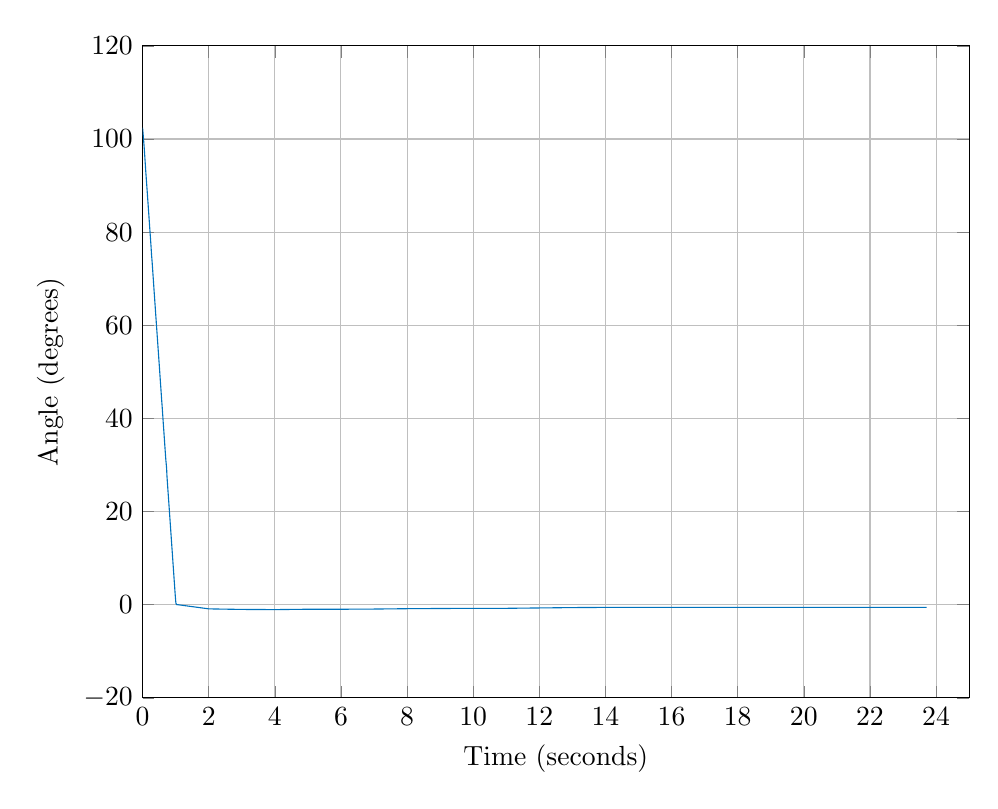
\begin{tikzpicture}

\begin{axis}[%
width=4.133in,
height=3.26in,
at={(0.693in,0.44in)},
scale only axis,
xmin=0,
xmax=25,
xmajorgrids,
xlabel={Time (seconds)},
ymin=-20,
ymax=120,
ymajorgrids,
ylabel={Angle (degrees)},
axis background/.style={fill=white}
]
\addplot [color=mycolor1,solid,forget plot]
  table[row sep=crcr]{%
0	102.4204\\
0.0159729680000003	101.2204\\
0.0319338129990008	99.7864\\
0.0502433389999997	98.1224\\
0.0655789880010001	96.4644\\
0.0807258700009994	94.8704\\
0.0960729890000001	93.1724\\
0.112036055	91.5504\\
0.128161949000001	89.9704\\
0.144050576001	88.3844\\
0.160048921	86.7724\\
0.176030784	85.1344\\
0.192037739	83.4984\\
0.208037833001001	81.8664\\
0.224080819	80.2304\\
0.240647512	78.5704\\
0.2566214	76.9364\\
0.271896785	75.1744\\
0.289959384	73.5664\\
0.305120738	72.0124\\
0.320473889001001	70.3924\\
0.336152263	68.7684\\
0.35205965	67.0584\\
0.368188445	65.4624\\
0.384014342	63.8324\\
0.400228368001999	62.1424\\
0.416159189999999	60.5164\\
0.432085597999999	58.9104\\
0.448031429	57.2844\\
0.464044958001001	55.6684\\
0.480174381000001	54.0164\\
0.496318912	52.3804\\
0.512599929	50.7304\\
0.527921844000001	49.1344\\
0.544017256000001	47.4624\\
0.560180254000001	45.8324\\
0.576298661	44.1364\\
0.593196734999999	42.5344\\
0.608588064999999	40.8964\\
0.624195044	39.2444\\
0.640184544	37.6464\\
0.656180279000999	36.0064\\
0.672107728	34.3324\\
0.688044904999001	32.7364\\
0.7040456	31.1184\\
0.727892064000999	29.3164\\
0.736705629000001	27.8384\\
0.751928787	26.2104\\
0.767997738	24.5684\\
0.784059498	22.9724\\
0.800123871999999	21.3264\\
0.816119843	19.6824\\
0.832162914000001	18.0524\\
0.848257537	16.4144\\
0.864159744000001	14.7664\\
0.880177794	13.1164\\
0.896201171	11.5044\\
0.912173548	9.84440000000001\\
0.928106915999999	8.20239999999998\\
0.944051464	6.5744\\
0.960030532	4.9444\\
0.975941729	3.3124\\
0.992198374	1.6644\\
1.008069146001	0.368399999999994\\
1.025285771001	0.0304000000000002\\
1.040631098	0.0183999999999997\\
1.056244704	0.00239999999999441\\
1.07214171	-0.0136000000000251\\
1.088198629	-0.0276000000000067\\
1.104168625	-0.0436000000000121\\
1.120169255	-0.0576000000000079\\
1.136249120001	-0.0736000000000132\\
1.152195566001	-0.0896000000000186\\
1.168239512	-0.1036\\
1.184157565	-0.11760000000001\\
1.200209472001	-0.133600000000001\\
1.216207621	-0.149600000000007\\
1.233590443	-0.165600000000012\\
1.248644794	-0.179600000000008\\
1.264212366999	-0.193600000000018\\
1.280020071	-0.209599999999995\\
1.296079306	-0.225600000000014\\
1.312044006	-0.24160000000002\\
1.328083108	-0.255600000000001\\
1.343942816001	-0.269600000000011\\
1.359878433	-0.287599999999998\\
1.375894442	-0.301600000000008\\
1.391888523	-0.317600000000013\\
1.407872942	-0.331600000000009\\
1.423950464	-0.345600000000019\\
1.440067251	-0.361599999999996\\
1.455965318	-0.377600000000001\\
1.47210815	-0.393600000000021\\
1.48795017	-0.407600000000002\\
1.506062087001	-0.423600000000008\\
1.521448853	-0.437600000000003\\
1.536945785	-0.453600000000009\\
1.552241413001	-0.469600000000014\\
1.568209735	-0.483599999999996\\
1.584196173001	-0.499600000000015\\
1.600056696001	-0.513600000000025\\
1.616119856	-0.529600000000002\\
1.632294262001	-0.545600000000007\\
1.648174861	-0.561599999999999\\
1.664222372	-0.573600000000013\\
1.680188409	-0.589600000000019\\
1.696138361	-0.60560000000001\\
1.712164543	-0.621600000000015\\
1.729855504	-0.637599999999992\\
1.74515857	-0.649600000000007\\
1.760145671	-0.665600000000012\\
1.775955012001	-0.681600000000003\\
1.792227992	-0.697600000000008\\
1.808244009	-0.713600000000014\\
1.824064932	-0.72760000000001\\
1.840171537	-0.74160000000002\\
1.856218914	-0.757599999999996\\
1.872072134	-0.773600000000016\\
1.888187535	-0.789600000000021\\
1.90428301	-0.803600000000003\\
1.920283515	-0.817600000000013\\
1.936059788	-0.833600000000004\\
1.952048952	-0.849600000000009\\
1.968049527	-0.865600000000015\\
1.983992351	-0.879600000000011\\
1.999911782	-0.893600000000021\\
2.018029829	-0.907600000000002\\
2.033238607	-0.907600000000002\\
2.048407894001	-0.907600000000002\\
2.064055064001	-0.909599999999998\\
2.080043822	-0.913600000000002\\
2.096051364001	-0.913600000000002\\
2.112032725	-0.915599999999998\\
2.128172832	-0.919600000000017\\
2.144050098	-0.919600000000017\\
2.160089311001	-0.921600000000012\\
2.176176998	-0.925600000000003\\
2.192200640999	-0.925600000000003\\
2.208059731	-0.927600000000012\\
2.224174314	-0.931600000000003\\
2.240022239	-0.931600000000003\\
2.255994543	-0.933599999999998\\
2.271962354	-0.937600000000003\\
2.287983199	-0.937600000000003\\
2.304122484999	-0.939599999999999\\
2.320042120001	-0.943599999999989\\
2.33619757	-0.943599999999989\\
2.352188944999	-0.943599999999989\\
2.368582841	-0.949600000000004\\
2.384035385001	-0.949600000000004\\
2.39999378	-0.949600000000004\\
2.416054346	-0.951600000000013\\
2.432015367	-0.955600000000004\\
2.448095998001	-0.955600000000004\\
2.464138544	-0.957599999999999\\
2.48003791	-0.961600000000004\\
2.495950976	-0.961600000000004\\
2.511970052001	-0.9636\\
2.528181568	-0.96759999999999\\
2.544197863	-0.96759999999999\\
2.560149658001	-0.969600000000014\\
2.576061837	-0.973600000000005\\
2.592281186001	-0.973600000000005\\
2.608041285	-0.975600000000014\\
2.624130065	-0.979600000000005\\
2.640031524999	-0.979600000000005\\
2.656034291	-0.9816\\
2.672098921	-0.985600000000005\\
2.688035757001	-0.985600000000005\\
2.704049291999	-0.985600000000005\\
2.720130525	-0.9876\\
2.736532177	-0.991599999999991\\
2.752030173	-0.991599999999991\\
2.768011472	-0.993599999999986\\
2.784275828	-0.997600000000006\\
2.800135006	-0.997600000000006\\
2.816238265999	-0.999600000000015\\
2.832184658001	-1.00360000000001\\
2.848202079	-1.00360000000001\\
2.864174325	-1.0056\\
2.880158501	-1.00960000000001\\
2.896135857	-1.00960000000001\\
2.912019936	-1.0116\\
2.928155133	-1.01560000000002\\
2.944247065	-1.01560000000002\\
2.960164733	-1.01760000000002\\
2.976062095001	-1.02160000000001\\
2.992004368	-1.02160000000001\\
3.007953966	-1.01960000000001\\
3.025479115	-1.02360000000002\\
3.040719209	-1.02360000000002\\
3.056066309	-1.02160000000001\\
3.072081187	-1.02360000000002\\
3.08801676	-1.02560000000001\\
3.104056173	-1.02560000000001\\
3.120037385	-1.02560000000001\\
3.136031721	-1.02760000000001\\
3.152059533001	-1.02760000000001\\
3.168061456	-1.02760000000001\\
3.18403932	-1.0296\\
3.200030544	-1.0296\\
3.216225229001	-1.0296\\
3.232017183	-1.0316\\
3.247994805	-1.0316\\
3.266081787	-1.0316\\
3.281550773	-1.03360000000001\\
3.296781978	-1.03360000000001\\
3.312188638	-1.03360000000001\\
3.328071805	-1.0356\\
3.344070069999	-1.0356\\
3.360182644001	-1.03360000000001\\
3.376186768	-1.03360000000001\\
3.392219595999	-1.03760000000003\\
3.408185102001	-1.03560000000002\\
3.424089102999	-1.03760000000003\\
3.440192942	-1.03960000000002\\
3.456147103	-1.03960000000002\\
3.476276741001	-1.03959999999999\\
3.488050213999	-1.04160000000002\\
3.504212498001	-1.04160000000002\\
3.51998871	-1.04159999999999\\
3.535912234	-1.0436\\
3.552115598	-1.0436\\
3.568058533001	-1.0436\\
3.584035722	-1.04559999999999\\
3.600212326	-1.04559999999999\\
3.616187404	-1.04560000000001\\
3.632180788	-1.04760000000002\\
3.648263174	-1.04760000000002\\
3.66417606	-1.04560000000001\\
3.68017186	-1.04760000000002\\
3.696179336	-1.04960000000001\\
3.712171001	-1.04760000000002\\
3.729286257001	-1.04960000000001\\
3.744296627	-1.05160000000001\\
3.759949635	-1.05160000000001\\
3.776025644	-1.05160000000001\\
3.79243516	-1.0536\\
3.808061738001	-1.0536\\
3.824233371	-1.0536\\
3.840180605	-1.0556\\
3.856178189	-1.0556\\
3.872188361	-1.0556\\
3.888158657	-1.05760000000001\\
3.904183363001	-1.05760000000001\\
3.920177844	-1.05760000000001\\
3.936154620001	-1.0596\\
3.952159566001	-1.0596\\
3.96817319	-1.0596\\
3.985026427001	-1.0616\\
3.999962639001	-1.0616\\
4.015934122	-1.0596\\
4.032031366	-1.05760000000001\\
4.048092037	-1.05760000000001\\
4.064263144	-1.0556\\
4.080187005001	-1.0556\\
4.096047758	-1.0536\\
4.112093712	-1.0536\\
4.128037253	-1.05160000000001\\
4.144149446	-1.04959999999998\\
4.160372495001	-1.04959999999998\\
4.176183717	-1.04759999999999\\
4.192207374	-1.04559999999999\\
4.208212946	-1.04559999999999\\
4.227966453	-1.0436\\
4.24084297	-1.04159999999999\\
4.255903446001	-1.04159999999999\\
4.273986179	-1.03959999999999\\
4.289203981	-1.0376\\
4.304420253	-1.0376\\
4.320216633001	-1.0356\\
4.33637252	-1.03360000000001\\
4.352049437	-1.03360000000001\\
4.368082681	-1.0316\\
4.384032913	-1.0296\\
4.40004105	-1.0296\\
4.416015085	-1.0296\\
4.432031952	-1.02760000000001\\
4.448049737	-1.02559999999998\\
4.464039708001	-1.02559999999998\\
4.482074767001	-1.02359999999999\\
4.497084121	-1.02159999999999\\
4.512021607	-1.02159999999999\\
4.527972196	-1.0196\\
4.543941799	-1.01759999999999\\
4.559896918001	-1.01759999999999\\
4.576152891	-1.01559999999999\\
4.592043393	-1.0136\\
4.608124328	-1.0136\\
4.62405134	-1.0116\\
4.64013372	-1.00960000000001\\
4.656121552	-1.00960000000001\\
4.672036949	-1.0076\\
4.688038486	-1.0056\\
4.704034807	-1.0056\\
4.720143939001	-1.0056\\
4.735906383	-1.00360000000001\\
4.754073761	-1.00159999999998\\
4.770136309	-1.00159999999998\\
4.785571488001	-0.999599999999987\\
4.800983084	-0.997599999999991\\
4.816422589	-0.997599999999991\\
4.832274072	-0.995599999999996\\
4.848198164	-0.993599999999986\\
4.864177461	-0.993599999999986\\
4.880195099001	-0.991599999999991\\
4.896159187001	-0.989599999999996\\
4.912127449999	-0.989599999999996\\
4.928038828	-0.9876\\
4.944039503	-0.985600000000005\\
4.96004975	-0.985600000000005\\
4.976112186001	-0.983599999999996\\
4.991999217	-0.9816\\
5.010145583	-0.9816\\
5.025292076	-0.9816\\
5.040580172001	-0.9816\\
5.056208028	-0.9816\\
5.072187366	-0.9816\\
5.08828907	-0.9816\\
5.104217176	-0.9816\\
5.120175716	-0.9816\\
5.136203864	-0.9816\\
5.152158590001	-0.9816\\
5.168132064001	-0.9816\\
5.184163715001	-0.9816\\
5.200209267	-0.9816\\
5.216061066001	-0.9816\\
5.232149069001	-0.9816\\
5.248044621001	-0.9816\\
5.264006537	-0.9816\\
5.279895171	-0.9816\\
5.296146479	-0.9816\\
5.31230402	-0.9816\\
5.328191812001	-0.9816\\
5.344121886	-0.9816\\
5.360203615	-0.9816\\
5.376180657	-0.9816\\
5.392042773	-0.9816\\
5.408452711	-0.9816\\
5.424190481	-0.9816\\
5.440145232999	-0.9816\\
5.456187783001	-0.9816\\
5.472121918001	-0.9816\\
5.489033858	-0.9816\\
5.504020137001	-0.9816\\
5.51995627	-0.9816\\
5.538209002	-0.9816\\
5.553528814001	-0.9816\\
5.569029943	-0.9816\\
5.584494414999	-0.9816\\
5.600321371	-0.9816\\
5.616220803	-0.9816\\
5.632055603	-0.9816\\
5.648776329	-0.9816\\
5.664058871	-0.9816\\
5.680034106001	-0.9816\\
5.6960119	-0.9816\\
5.712358840001	-0.9816\\
5.730011721	-0.9816\\
5.74412545	-0.9816\\
5.760327879	-0.9816\\
5.777762916	-0.9816\\
5.793189452	-0.9816\\
5.80869458	-0.9816\\
5.824150672	-0.9816\\
5.840040631	-0.9816\\
5.856046103	-0.9816\\
5.872099302	-0.9816\\
5.890645178	-0.9816\\
5.906185481	-0.9816\\
5.921747453	-0.9816\\
5.937107878	-0.9816\\
5.952485733	-0.9816\\
5.968051538	-0.9816\\
5.983990609001	-0.9816\\
6.000069857001	-0.9816\\
6.016292089	-0.9816\\
6.032071739	-0.979600000000005\\
6.048296157	-0.979600000000005\\
6.064169956	-0.979600000000005\\
6.080015525	-0.979600000000005\\
6.096201921	-0.97760000000001\\
6.112070735	-0.97760000000001\\
6.128040774	-0.97760000000001\\
6.144189224001	-0.975600000000014\\
6.160037374	-0.975600000000014\\
6.176109328001	-0.975600000000014\\
6.192160399	-0.973600000000005\\
6.208192397	-0.973600000000005\\
6.224336588	-0.973600000000005\\
6.23994943	-0.971600000000009\\
6.258101535	-0.971600000000009\\
6.273467481001	-0.971600000000009\\
6.289028978	-0.969599999999986\\
6.304498325	-0.969599999999986\\
6.320191393	-0.969599999999986\\
6.336107232	-0.96759999999999\\
6.352148139001	-0.96759999999999\\
6.368181719	-0.96759999999999\\
6.384218266	-0.965599999999995\\
6.400195473	-0.965599999999995\\
6.416187594	-0.965599999999995\\
6.432171256	-0.965599999999995\\
6.448150683	-0.9636\\
6.464158300001	-0.9636\\
6.481555761	-0.9636\\
6.496534606001	-0.961600000000004\\
6.511933971	-0.961600000000004\\
6.527970923	-0.961600000000004\\
6.544149455	-0.959599999999995\\
6.560053862	-0.959599999999995\\
6.575997260999	-0.959599999999995\\
6.594282805001	-0.957599999999999\\
6.609756506	-0.957599999999999\\
6.62505428	-0.957599999999999\\
6.640139797	-0.955600000000004\\
6.656078337	-0.955600000000004\\
6.672082726	-0.955600000000004\\
6.688033744	-0.953600000000009\\
6.704035477	-0.953600000000009\\
6.720083369	-0.953600000000009\\
6.736369878	-0.953600000000009\\
6.752016216	-0.951600000000013\\
6.767966866	-0.951600000000013\\
6.784039221	-0.951600000000013\\
6.80005026	-0.949600000000004\\
6.816245626	-0.949600000000004\\
6.83225245	-0.949600000000004\\
6.848169351	-0.947600000000008\\
6.864157373001	-0.947600000000008\\
6.880229676	-0.947600000000008\\
6.896051046	-0.945599999999985\\
6.912286864	-0.945599999999985\\
6.928233462001	-0.945599999999985\\
6.944250970001	-0.943599999999989\\
6.960184499	-0.943599999999989\\
6.978704118	-0.943599999999989\\
6.993743258	-0.941599999999994\\
7.009115177001	-0.941599999999994\\
7.023913989999	-0.941599999999994\\
7.040149615	-0.939599999999999\\
7.056045032	-0.937600000000003\\
7.072053345	-0.937600000000003\\
7.088034687	-0.937600000000003\\
7.104086914	-0.933599999999998\\
7.120034695	-0.933599999999998\\
7.136046529999	-0.933599999999998\\
7.152039604	-0.929600000000008\\
7.168012226	-0.929600000000008\\
7.183988957	-0.929600000000008\\
7.199999756	-0.925599999999989\\
7.215996848	-0.925599999999989\\
7.232039903	-0.925599999999989\\
7.247993297001	-0.921599999999984\\
7.263971508	-0.921599999999984\\
7.279918161	-0.921599999999984\\
7.295932783001	-0.917599999999993\\
7.311912627	-0.917599999999993\\
7.327922337001	-0.917599999999993\\
7.343908164999	-0.913600000000002\\
7.359920481001	-0.913600000000002\\
7.375961985	-0.913600000000002\\
7.392040226	-0.913600000000002\\
7.408335884	-0.909599999999998\\
7.424076336	-0.909599999999998\\
7.440035221	-0.909599999999998\\
7.456165529999	-0.905600000000007\\
7.471912	-0.905600000000007\\
7.489031093	-0.905600000000007\\
7.504691260001	-0.901600000000002\\
7.520037116	-0.901600000000002\\
7.536157297	-0.901600000000002\\
7.552317769001	-0.897599999999983\\
7.5681815	-0.897599999999983\\
7.583995232001	-0.897599999999983\\
7.599960107	-0.893599999999992\\
7.615939895	-0.893599999999992\\
7.631991546	-0.893599999999992\\
7.647936524001	-0.891599999999997\\
7.663933282	-0.889600000000002\\
7.679933324	-0.889600000000002\\
7.695940539999	-0.889600000000002\\
7.711883441001	-0.885599999999997\\
7.730128201	-0.885599999999997\\
7.745170319999	-0.885599999999997\\
7.760205227	-0.881600000000006\\
7.776058318	-0.881600000000006\\
7.79200196	-0.881600000000006\\
7.808074282	-0.877600000000001\\
7.824198801	-0.877600000000001\\
7.840164805	-0.877600000000001\\
7.856042889	-0.873599999999982\\
7.872023193	-0.873599999999982\\
7.888020640999	-0.873599999999982\\
7.904039899001	-0.869599999999991\\
7.920161177	-0.869599999999991\\
7.936024056	-0.869599999999991\\
7.951991581	-0.865600000000001\\
7.96799389	-0.865600000000001\\
7.986729956	-0.865600000000001\\
8.000056338999	-0.863599999999991\\
8.015943756	-0.861599999999996\\
8.031934898	-0.861599999999996\\
8.047952063	-0.861599999999996\\
8.063983156001	-0.8596\\
8.0801402	-0.8596\\
8.096036655	-0.8596\\
8.112039404999	-0.857600000000005\\
8.128030584	-0.857600000000005\\
8.144195101	-0.857600000000005\\
8.160147031	-0.85560000000001\\
8.176041416	-0.85560000000001\\
8.19204389	-0.85560000000001\\
8.208028424	-0.8536\\
8.224041097	-0.8536\\
8.239959869	-0.8536\\
8.258049312	-0.851600000000005\\
8.272963982999	-0.851600000000005\\
8.288363278	-0.851600000000005\\
8.304027551	-0.849599999999981\\
8.320189389001	-0.849599999999981\\
8.336194046	-0.849599999999981\\
8.352220099001	-0.849599999999981\\
8.368166557001	-0.847599999999986\\
8.384198123	-0.847599999999986\\
8.400185192001	-0.847599999999986\\
8.415990348	-0.84559999999999\\
8.432110029999	-0.84559999999999\\
8.448043814	-0.84559999999999\\
8.464001041	-0.843599999999995\\
8.480098389001	-0.843599999999995\\
8.49595773	-0.843599999999995\\
8.511939935	-0.8416\\
8.528033467	-0.8416\\
8.54418576	-0.8416\\
8.560191192	-0.83959999999999\\
8.576160892001	-0.83959999999999\\
8.592101862	-0.83959999999999\\
8.608067093	-0.837599999999995\\
8.624074227001	-0.837599999999995\\
8.640265354001	-0.837599999999995\\
8.656172954	-0.837599999999995\\
8.672179022	-0.835599999999999\\
8.688210989	-0.835599999999999\\
8.704295103	-0.835599999999999\\
8.720142331	-0.833600000000004\\
8.736064104	-0.833600000000004\\
8.752008265999	-0.833600000000004\\
8.769340121	-0.831600000000009\\
8.784556934	-0.831600000000009\\
8.80006042	-0.831600000000009\\
8.815977016	-0.829599999999999\\
8.832184876	-0.829599999999999\\
8.848172476	-0.829599999999999\\
8.864250362	-0.827600000000004\\
8.880142687	-0.827600000000004\\
8.896181308	-0.827600000000004\\
8.91214505	-0.825600000000009\\
8.927992014001	-0.825600000000009\\
8.944189659	-0.825600000000009\\
8.960184738001	-0.823599999999985\\
8.976068232001	-0.823599999999985\\
8.992207513	-0.823599999999985\\
9.008028939	-0.823599999999985\\
9.025214451	-0.821599999999989\\
9.041485206	-0.821599999999989\\
9.056331349001	-0.821599999999989\\
9.07187652	-0.819599999999994\\
9.087947407	-0.819599999999994\\
9.10416093	-0.819599999999994\\
9.120098493002	-0.817599999999999\\
9.13608466	-0.817599999999999\\
9.152058394001	-0.817599999999999\\
9.16804151	-0.815599999999989\\
9.184031206	-0.815599999999989\\
9.200034412	-0.815599999999989\\
9.215962844	-0.813599999999994\\
9.234431173	-0.813599999999994\\
9.249515239001	-0.813599999999994\\
9.264520604	-0.811599999999999\\
9.280567420001	-0.811599999999999\\
9.296168811001	-0.811599999999999\\
9.312077217	-0.811599999999999\\
9.328065991	-0.809600000000003\\
9.34392414	-0.809600000000003\\
9.36000381	-0.809600000000003\\
9.376067872	-0.807600000000008\\
9.392070663	-0.807600000000008\\
9.408038319	-0.807600000000008\\
9.424044376	-0.805599999999998\\
9.440070344	-0.805599999999998\\
9.456039017	-0.805599999999998\\
9.472044373001	-0.803600000000003\\
9.48824116	-0.803600000000003\\
9.50395095	-0.803600000000003\\
9.519983256	-0.801600000000008\\
9.536050452	-0.801600000000008\\
9.552020304	-0.801600000000008\\
9.567995572	-0.799599999999984\\
9.58418366	-0.799599999999984\\
9.600172355	-0.799599999999984\\
9.616129588001	-0.799599999999984\\
9.632222733	-0.797599999999989\\
9.648174227	-0.797599999999989\\
9.664222661001	-0.797599999999989\\
9.680047272	-0.795599999999993\\
9.696154268	-0.795599999999993\\
9.712168199001	-0.795599999999993\\
9.731033397999	-0.793599999999998\\
9.743936703001	-0.793599999999998\\
9.760006129	-0.793599999999998\\
9.775963502	-0.791599999999988\\
9.792140605	-0.791599999999988\\
9.808180946001	-0.791599999999988\\
9.824053092	-0.789599999999993\\
9.840107649	-0.789599999999993\\
9.856150069	-0.789599999999993\\
9.872158354001	-0.787599999999998\\
9.888461708	-0.787599999999998\\
9.904198043001	-0.787599999999998\\
9.920116953	-0.785600000000002\\
9.936171452	-0.785600000000002\\
9.952166794	-0.785600000000002\\
9.968483626	-0.785600000000002\\
9.984090613	-0.783600000000007\\
9.999948186	-0.783600000000007\\
10.015970784	-0.783600000000007\\
10.032010647999	-0.783600000000007\\
10.048125989	-0.783600000000007\\
10.064043275	-0.783600000000007\\
10.080173414	-0.783600000000007\\
10.096143449999	-0.783600000000007\\
10.112138638	-0.783600000000007\\
10.128084835	-0.783600000000007\\
10.144064844	-0.783600000000007\\
10.160035381	-0.783600000000007\\
10.176035495001	-0.783600000000007\\
10.191997844	-0.783600000000007\\
10.208004293001	-0.783600000000007\\
10.224326487	-0.783600000000007\\
10.239945812999	-0.783600000000007\\
10.255898808	-0.783600000000007\\
10.273927475	-0.783600000000007\\
10.289326178	-0.783600000000007\\
10.304785521001	-0.783600000000007\\
10.320255687001	-0.783600000000007\\
10.336069506999	-0.783600000000007\\
10.352138027	-0.783600000000007\\
10.368045857	-0.783600000000007\\
10.384180461	-0.783600000000007\\
10.400172126	-0.783600000000007\\
10.416183511	-0.783600000000007\\
10.432161846	-0.783600000000007\\
10.448173581	-0.783600000000007\\
10.464140005	-0.783600000000007\\
10.482287107	-0.783600000000007\\
10.497495508	-0.783600000000007\\
10.512497438	-0.783600000000007\\
10.527972957	-0.783600000000007\\
10.544142342	-0.783600000000007\\
10.560031424	-0.783600000000007\\
10.576141517	-0.783600000000007\\
10.592037599001	-0.783600000000007\\
10.609671774001	-0.783600000000007\\
10.625008131	-0.783600000000007\\
10.640402804	-0.783600000000007\\
10.656164118	-0.783600000000007\\
10.672190235	-0.783600000000007\\
10.688186951999	-0.783600000000007\\
10.704059006	-0.783600000000007\\
10.720090631999	-0.783600000000007\\
10.737150978	-0.783600000000007\\
10.752113685	-0.783600000000007\\
10.768130469	-0.783600000000007\\
10.784190159	-0.783600000000007\\
10.800178982	-0.783600000000007\\
10.816039807	-0.783600000000007\\
10.832205776	-0.783600000000007\\
10.848187659	-0.783600000000007\\
10.864180918	-0.783600000000007\\
10.880154442	-0.783600000000007\\
10.896027057	-0.783600000000007\\
10.912025432	-0.783600000000007\\
10.928178964	-0.783600000000007\\
10.944048247	-0.783600000000007\\
10.960043155	-0.783600000000007\\
10.976052119	-0.783600000000007\\
10.991908186001	-0.783600000000007\\
11.009988561001	-0.783600000000007\\
11.024827267	-0.781599999999997\\
11.040053674	-0.781599999999997\\
11.056133254	-0.779600000000002\\
11.071945234	-0.777600000000007\\
11.088052543001	-0.777600000000007\\
11.104075544	-0.775600000000011\\
11.120025890999	-0.773600000000016\\
11.136094986001	-0.773600000000016\\
11.152140268	-0.771599999999992\\
11.168063062	-0.771599999999992\\
11.184063553	-0.769599999999997\\
11.200038209	-0.767599999999987\\
11.216081871999	-0.767599999999987\\
11.233141331	-0.765599999999992\\
11.248102499	-0.763599999999997\\
11.264532299	-0.763599999999997\\
11.28046865	-0.761600000000001\\
11.296037792	-0.759600000000006\\
11.312032419	-0.759600000000006\\
11.32807544	-0.757599999999996\\
11.344099539	-0.757599999999996\\
11.360080856	-0.755600000000001\\
11.376117838	-0.753600000000006\\
11.392005031999	-0.753600000000006\\
11.407996948001	-0.75160000000001\\
11.423986117	-0.749600000000015\\
11.439995112	-0.749600000000015\\
11.456184379	-0.747599999999991\\
11.472182914999	-0.745599999999996\\
11.48874183	-0.745599999999996\\
11.504025692	-0.743599999999986\\
11.52000991	-0.743599999999986\\
11.537708722	-0.741599999999991\\
11.552966781	-0.739599999999996\\
11.568401765	-0.739599999999996\\
11.584237572	-0.7376\\
11.600469782	-0.735600000000005\\
11.616164284	-0.735600000000005\\
11.63195769	-0.733599999999996\\
11.648231958001	-0.7316\\
11.664316586	-0.7316\\
11.680126991001	-0.729600000000005\\
11.696190902	-0.729600000000005\\
11.712149256999	-0.72760000000001\\
11.728108416	-0.725600000000014\\
11.744023636	-0.725600000000014\\
11.760030853	-0.723600000000005\\
11.776023827	-0.721600000000009\\
11.792174617	-0.721600000000009\\
11.808222775	-0.719599999999986\\
11.824165219	-0.71759999999999\\
11.840304378	-0.71759999999999\\
11.856361090001	-0.715599999999995\\
11.872149601	-0.715599999999995\\
11.888234397	-0.7136\\
11.904271685	-0.711600000000004\\
11.920044645	-0.711600000000004\\
11.936016074	-0.709599999999995\\
11.952178972001	-0.707599999999999\\
11.968195844	-0.707599999999999\\
11.986078922001	-0.705600000000004\\
12.001339043	-0.703600000000009\\
12.016265316001	-0.703600000000009\\
12.031931226	-0.701600000000013\\
12.048009648	-0.701600000000013\\
12.064169068	-0.699600000000004\\
12.080301652	-0.697600000000008\\
12.096156818	-0.697600000000008\\
12.112174407	-0.695599999999985\\
12.128041014001	-0.695599999999985\\
12.144153206999	-0.693599999999989\\
12.160394543	-0.691599999999994\\
12.17624791	-0.691599999999994\\
12.192154627	-0.689599999999999\\
12.208275019001	-0.687600000000003\\
12.224158870001	-0.687600000000003\\
12.241515324	-0.685599999999994\\
12.256561543	-0.683599999999998\\
12.271960162	-0.683599999999998\\
12.288213384	-0.681600000000003\\
12.304176435	-0.679600000000008\\
12.320179792	-0.679600000000008\\
12.336184627	-0.677600000000012\\
12.352190143	-0.677600000000012\\
12.368177694001	-0.675600000000003\\
12.384239172001	-0.673600000000008\\
12.400161661	-0.673600000000008\\
12.416221645	-0.671599999999984\\
12.432234704	-0.669599999999988\\
12.448051949	-0.669599999999988\\
12.464163681	-0.667599999999993\\
12.484072635	-0.667599999999993\\
12.496366747	-0.665599999999998\\
12.512473144001	-0.663600000000002\\
12.527935561001	-0.663600000000002\\
12.545973069999	-0.661599999999993\\
12.561401297001	-0.659599999999998\\
12.57681111	-0.659599999999998\\
12.592598188	-0.657600000000002\\
12.6080558	-0.655600000000007\\
12.624212893	-0.655600000000007\\
12.640194465	-0.653600000000012\\
12.656215081	-0.651600000000002\\
12.672189156001	-0.651600000000002\\
12.688070962001	-0.649600000000007\\
12.704157442	-0.649600000000007\\
12.72012356	-0.647599999999983\\
12.738214099001	-0.645599999999988\\
12.752076411	-0.645599999999988\\
12.768067005	-0.643599999999992\\
12.783932413001	-0.641599999999997\\
12.799947800001	-0.641599999999997\\
12.816190205	-0.639600000000002\\
12.83222166	-0.639600000000002\\
12.848154417	-0.637599999999992\\
12.864182625	-0.635599999999997\\
12.880251475	-0.635599999999997\\
12.896192315	-0.633600000000001\\
12.912158292	-0.631600000000006\\
12.928052942	-0.631600000000006\\
12.944049974001	-0.629600000000011\\
12.96004431	-0.627600000000001\\
12.976027566001	-0.627600000000001\\
12.992043908001	-0.625600000000006\\
13.007992924	-0.625600000000006\\
13.023989373	-0.625600000000006\\
13.040009656	-0.62360000000001\\
13.056184661999	-0.62360000000001\\
13.072210540001	-0.62360000000001\\
13.088196963999	-0.621599999999987\\
13.104192456	-0.621599999999987\\
13.120185407	-0.621599999999987\\
13.136173441001	-0.621599999999987\\
13.15217505	-0.619599999999991\\
13.168176858	-0.619599999999991\\
13.184172196001	-0.619599999999991\\
13.200043107999	-0.617599999999996\\
13.216181846	-0.617599999999996\\
13.235255373	-0.617599999999996\\
13.247900283001	-0.615600000000001\\
13.263955441001	-0.615600000000001\\
13.279950710002	-0.615600000000001\\
13.296181447	-0.613599999999991\\
13.312222072	-0.613599999999991\\
13.328359680001	-0.613599999999991\\
13.344152947999	-0.611599999999996\\
13.360052109001	-0.611599999999996\\
13.376032123001	-0.611599999999996\\
13.392034982999	-0.6096\\
13.408367084	-0.6096\\
13.424261294	-0.6096\\
13.440187621	-0.607600000000005\\
13.456383188	-0.607600000000005\\
13.47228053	-0.607600000000005\\
13.489396531001	-0.607600000000005\\
13.505576413001	-0.60560000000001\\
13.520455183	-0.60560000000001\\
13.536028725	-0.60560000000001\\
13.552175215999	-0.6036\\
13.568304359	-0.6036\\
13.584071399001	-0.6036\\
13.600187080001	-0.601600000000005\\
13.616186798	-0.601600000000005\\
13.632163088001	-0.601600000000005\\
13.648176859001	-0.599600000000009\\
13.664333242	-0.599600000000009\\
13.680238236001	-0.599600000000009\\
13.69617643	-0.597600000000014\\
13.712174966	-0.597600000000014\\
13.728322499	-0.597600000000014\\
13.745056606	-0.59559999999999\\
13.760624085002	-0.59559999999999\\
13.777398955	-0.59559999999999\\
13.792420245	-0.59559999999999\\
13.808225072999	-0.593599999999995\\
13.824291929	-0.593599999999995\\
13.840047925	-0.593599999999995\\
13.856041269	-0.5916\\
13.872033305	-0.5916\\
13.888039789	-0.5916\\
13.904040279	-0.58959999999999\\
13.920015086	-0.58959999999999\\
13.936008564001	-0.58959999999999\\
13.952116689	-0.587599999999995\\
13.968042951	-0.587599999999995\\
13.984121703	-0.587599999999995\\
13.99992643	-0.585599999999999\\
14.017126861001	-0.585599999999999\\
14.032133811001	-0.585599999999999\\
14.047897722001	-0.585599999999999\\
14.063960238	-0.585599999999999\\
14.080229802001	-0.585599999999999\\
14.096056253	-0.585599999999999\\
14.112028154	-0.585599999999999\\
14.128039433	-0.585599999999999\\
14.144070317	-0.585599999999999\\
14.160044112	-0.585599999999999\\
14.176016994	-0.585599999999999\\
14.192043995001	-0.585599999999999\\
14.208043879	-0.585599999999999\\
14.22404493	-0.585599999999999\\
14.240166553	-0.585599999999999\\
14.256026214	-0.585599999999999\\
14.271945394001	-0.585599999999999\\
14.287959192	-0.585599999999999\\
14.304090668999	-0.585599999999999\\
14.320067074	-0.585599999999999\\
14.336073658001	-0.585599999999999\\
14.352013356	-0.585599999999999\\
14.367991545001	-0.585599999999999\\
14.383992291	-0.585599999999999\\
14.399990164999	-0.585599999999999\\
14.416042852999	-0.585599999999999\\
14.432047052	-0.585599999999999\\
14.448024164	-0.585599999999999\\
14.46404061	-0.585599999999999\\
14.480043651	-0.585599999999999\\
14.495906952	-0.585599999999999\\
14.512016565	-0.585599999999999\\
14.527977513	-0.585599999999999\\
14.543893447	-0.585599999999999\\
14.560011688	-0.585599999999999\\
14.576205191001	-0.585599999999999\\
14.592175288	-0.585599999999999\\
14.608232677001	-0.585599999999999\\
14.62421894	-0.585599999999999\\
14.640370557001	-0.585599999999999\\
14.656199108	-0.585599999999999\\
14.672188784	-0.585599999999999\\
14.688245491001	-0.585599999999999\\
14.704174324	-0.585599999999999\\
14.720193997	-0.585599999999999\\
14.736122568	-0.585599999999999\\
14.752019796	-0.585599999999999\\
14.768034377	-0.585599999999999\\
14.783915691001	-0.585599999999999\\
14.800160476	-0.585599999999999\\
14.816220406001	-0.585599999999999\\
14.832290218	-0.585599999999999\\
14.848169018	-0.585599999999999\\
14.864182899	-0.585599999999999\\
14.880185182	-0.585599999999999\\
14.896162024	-0.585599999999999\\
14.912160664999	-0.585599999999999\\
14.928055661001	-0.585599999999999\\
14.944023552	-0.585599999999999\\
14.960032272	-0.585599999999999\\
14.976051008	-0.585599999999999\\
14.991939251	-0.585599999999999\\
15.007951868	-0.585599999999999\\
15.025100583	-0.585599999999999\\
15.040487778001	-0.585599999999999\\
15.056136907	-0.585599999999999\\
15.072147746001	-0.585599999999999\\
15.088283483	-0.585599999999999\\
15.104189654	-0.585599999999999\\
15.120151617	-0.585599999999999\\
15.136156261	-0.585599999999999\\
15.152161788	-0.585599999999999\\
15.168331492	-0.585599999999999\\
15.18419665	-0.585599999999999\\
15.200158889001	-0.585599999999999\\
15.216178337001	-0.585599999999999\\
15.235760084	-0.585599999999999\\
15.24795061	-0.585599999999999\\
15.26604889	-0.585599999999999\\
15.281086479001	-0.585599999999999\\
15.296510965	-0.585599999999999\\
15.312066807	-0.585599999999999\\
15.328064622	-0.585599999999999\\
15.344075187	-0.585599999999999\\
15.360040373	-0.585599999999999\\
15.376062557	-0.585599999999999\\
15.392026772	-0.585599999999999\\
15.408005755001	-0.585599999999999\\
15.424035009	-0.585599999999999\\
15.440295293	-0.585599999999999\\
15.456192599001	-0.585599999999999\\
15.472213882001	-0.585599999999999\\
15.488088749	-0.585599999999999\\
15.505285696001	-0.585599999999999\\
15.520638631	-0.585599999999999\\
15.536150358	-0.585599999999999\\
15.552179693	-0.585599999999999\\
15.568052476	-0.585599999999999\\
15.584162093	-0.585599999999999\\
15.600525891	-0.585599999999999\\
15.61614409	-0.585599999999999\\
15.632177099001	-0.585599999999999\\
15.648173389	-0.585599999999999\\
15.664433979001	-0.585599999999999\\
15.680206247	-0.585599999999999\\
15.696167102	-0.585599999999999\\
15.712184941001	-0.585599999999999\\
15.728164559	-0.585599999999999\\
15.746060789	-0.585599999999999\\
15.7610405	-0.585599999999999\\
15.776132782	-0.585599999999999\\
15.791981589	-0.585599999999999\\
15.808024793001	-0.585599999999999\\
15.824217428	-0.585599999999999\\
15.840222097001	-0.585599999999999\\
15.856151631999	-0.585599999999999\\
15.872176107	-0.585599999999999\\
15.8881031	-0.585599999999999\\
15.904153474001	-0.585599999999999\\
15.920150485	-0.585599999999999\\
15.936174734	-0.585599999999999\\
15.952191712001	-0.585599999999999\\
15.96817134	-0.585599999999999\\
15.986342277	-0.585599999999999\\
16.000431818	-0.585599999999999\\
16.015879863001	-0.585599999999999\\
16.033919727	-0.585599999999999\\
16.049118385999	-0.585599999999999\\
16.064720729	-0.585599999999999\\
16.080212221	-0.585599999999999\\
16.096170581	-0.585599999999999\\
16.112176538	-0.585599999999999\\
16.128148333	-0.585599999999999\\
16.144161181	-0.585599999999999\\
16.160160078	-0.585599999999999\\
16.176173753	-0.585599999999999\\
16.19216401	-0.585599999999999\\
16.20817549	-0.585599999999999\\
16.224368075	-0.585599999999999\\
16.240903036	-0.585599999999999\\
16.255994651002	-0.585599999999999\\
16.27189487	-0.585599999999999\\
16.289916779001	-0.585599999999999\\
16.305228449	-0.585599999999999\\
16.320749357999	-0.585599999999999\\
16.336394433	-0.585599999999999\\
16.352166395	-0.585599999999999\\
16.368200777	-0.585599999999999\\
16.384063846	-0.585599999999999\\
16.400134636	-0.585599999999999\\
16.416039394001	-0.585599999999999\\
16.431980224001	-0.585599999999999\\
16.44803402	-0.585599999999999\\
16.464177403	-0.585599999999999\\
16.480459587001	-0.585599999999999\\
16.495958129	-0.585599999999999\\
16.511991442	-0.585599999999999\\
16.52851023	-0.585599999999999\\
16.544005182	-0.585599999999999\\
16.560179723	-0.585599999999999\\
16.576163449999	-0.585599999999999\\
16.592148836	-0.585599999999999\\
16.608078581	-0.585599999999999\\
16.624182956	-0.585599999999999\\
16.640207210002	-0.585599999999999\\
16.65638301	-0.585599999999999\\
16.672044851	-0.585599999999999\\
16.688027069	-0.585599999999999\\
16.704143565	-0.585599999999999\\
16.720185526002	-0.585599999999999\\
16.739536867	-0.585599999999999\\
16.753102627	-0.585599999999999\\
16.769114227	-0.585599999999999\\
16.784041905	-0.585599999999999\\
16.799949648	-0.585599999999999\\
16.815950317	-0.585599999999999\\
16.832178959	-0.585599999999999\\
16.848212866	-0.585599999999999\\
16.864178903001	-0.585599999999999\\
16.880163346	-0.585599999999999\\
16.896045458001	-0.585599999999999\\
16.912033991	-0.585599999999999\\
16.928041768	-0.585599999999999\\
16.944052792	-0.585599999999999\\
16.960036499	-0.585599999999999\\
16.976031968	-0.585599999999999\\
16.992044071001	-0.585599999999999\\
17.008003958	-0.585599999999999\\
17.025150875	-0.585599999999999\\
17.040755601	-0.585599999999999\\
17.056133197	-0.585599999999999\\
17.07215813	-0.585599999999999\\
17.088041337	-0.585599999999999\\
17.104154999	-0.585599999999999\\
17.120084523	-0.585599999999999\\
17.136036148	-0.585599999999999\\
17.152175628	-0.585599999999999\\
17.168186196	-0.585599999999999\\
17.184187217	-0.585599999999999\\
17.200181307001	-0.585599999999999\\
17.216202745	-0.585599999999999\\
17.232165249	-0.585599999999999\\
17.249706369	-0.585599999999999\\
17.265727972	-0.585599999999999\\
17.281865172001	-0.585599999999999\\
17.295915479	-0.585599999999999\\
17.312064887001	-0.585599999999999\\
17.328179245001	-0.585599999999999\\
17.344039488001	-0.585599999999999\\
17.360054145	-0.585599999999999\\
17.376043880001	-0.585599999999999\\
17.392019944999	-0.585599999999999\\
17.410266348	-0.585599999999999\\
17.425592079	-0.585599999999999\\
17.44109835	-0.585599999999999\\
17.456378844	-0.585599999999999\\
17.472081819999	-0.585599999999999\\
17.488815617	-0.585599999999999\\
17.504757717	-0.585599999999999\\
17.52061691	-0.585599999999999\\
17.537280781001	-0.585599999999999\\
17.552285132001	-0.585599999999999\\
17.568119043	-0.585599999999999\\
17.584010657	-0.585599999999999\\
17.600143397	-0.585599999999999\\
17.616186289	-0.585599999999999\\
17.632153097	-0.585599999999999\\
17.648151588	-0.585599999999999\\
17.664229669	-0.585599999999999\\
17.680101517	-0.585599999999999\\
17.696182715	-0.585599999999999\\
17.712264454	-0.585599999999999\\
17.728075907	-0.585599999999999\\
17.743904977001	-0.585599999999999\\
17.760042430999	-0.585599999999999\\
17.775958382001	-0.585599999999999\\
17.791922197	-0.585599999999999\\
17.807940616	-0.585599999999999\\
17.825992071	-0.585599999999999\\
17.841296685	-0.585599999999999\\
17.856793845	-0.585599999999999\\
17.872182241	-0.585599999999999\\
17.88822275	-0.585599999999999\\
17.90418567	-0.585599999999999\\
17.920152333	-0.585599999999999\\
17.936261499	-0.585599999999999\\
17.952190537	-0.585599999999999\\
17.96807957	-0.585599999999999\\
17.984555232	-0.585599999999999\\
18.00182841	-0.585599999999999\\
18.017758463	-0.585599999999999\\
18.033180591	-0.585599999999999\\
18.048651343	-0.585599999999999\\
18.064196304001	-0.585599999999999\\
18.080194138	-0.585599999999999\\
18.096203561001	-0.585599999999999\\
18.112151675	-0.585599999999999\\
18.12820078	-0.585599999999999\\
18.144080463001	-0.585599999999999\\
18.160173661	-0.585599999999999\\
18.176170478	-0.585599999999999\\
18.192336163	-0.585599999999999\\
18.208228663001	-0.585599999999999\\
18.224194811	-0.585599999999999\\
18.241160312	-0.585599999999999\\
18.256662022	-0.585599999999999\\
18.271971234	-0.585599999999999\\
18.287948212001	-0.585599999999999\\
18.30396016	-0.585599999999999\\
18.322177897	-0.585599999999999\\
18.337858668001	-0.585599999999999\\
18.353337621999	-0.585599999999999\\
18.368925788	-0.585599999999999\\
18.384370699	-0.585599999999999\\
18.400174028001	-0.585599999999999\\
18.416207011	-0.585599999999999\\
18.432055342	-0.585599999999999\\
18.448041064	-0.585599999999999\\
18.464038397	-0.585599999999999\\
18.480014226	-0.585599999999999\\
18.495955387	-0.585599999999999\\
18.512011218001	-0.585599999999999\\
18.527935648	-0.585599999999999\\
18.543887918001	-0.585599999999999\\
18.560010777	-0.585599999999999\\
18.576186027	-0.585599999999999\\
18.592114291	-0.585599999999999\\
18.608043444	-0.585599999999999\\
18.62401988	-0.585599999999999\\
18.64003581	-0.585599999999999\\
18.656149497	-0.585599999999999\\
18.672244426	-0.585599999999999\\
18.688173935	-0.585599999999999\\
18.704186703001	-0.585599999999999\\
18.720189478	-0.585599999999999\\
18.736504225	-0.585599999999999\\
18.751953586	-0.585599999999999\\
18.770093849001	-0.585599999999999\\
18.78509109	-0.585599999999999\\
18.800124126	-0.585599999999999\\
18.816171336	-0.585599999999999\\
18.832180882001	-0.585599999999999\\
18.848181555	-0.585599999999999\\
18.864139717	-0.585599999999999\\
18.880186296	-0.585599999999999\\
18.896229373001	-0.585599999999999\\
18.912053734	-0.585599999999999\\
18.928029689001	-0.585599999999999\\
18.944049506999	-0.585599999999999\\
18.960124406	-0.585599999999999\\
18.976047481001	-0.585599999999999\\
18.992607998	-0.585599999999999\\
19.009258444999	-0.585599999999999\\
19.025330249	-0.585599999999999\\
19.040559096	-0.585599999999999\\
19.056182778001	-0.585599999999999\\
19.072134234	-0.585599999999999\\
19.088204124	-0.585599999999999\\
19.104147937	-0.585599999999999\\
19.120142322	-0.585599999999999\\
19.136029370001	-0.585599999999999\\
19.152073143	-0.585599999999999\\
19.168180175001	-0.585599999999999\\
19.184182324001	-0.585599999999999\\
19.200045833	-0.585599999999999\\
19.216035128999	-0.585599999999999\\
19.232176523	-0.585599999999999\\
19.247993702	-0.585599999999999\\
19.263991276	-0.585599999999999\\
19.279963583	-0.585599999999999\\
19.296185238	-0.585599999999999\\
19.312055223	-0.585599999999999\\
19.328227733	-0.585599999999999\\
19.3441365	-0.585599999999999\\
19.360037565	-0.585599999999999\\
19.378304825	-0.585599999999999\\
19.393370893	-0.585599999999999\\
19.408425281	-0.585599999999999\\
19.42404777	-0.585599999999999\\
19.440001674	-0.585599999999999\\
19.456021408001	-0.585599999999999\\
19.472145703001	-0.585599999999999\\
19.490838618	-0.585599999999999\\
19.505829035	-0.585599999999999\\
19.521900472001	-0.585599999999999\\
19.536804136	-0.585599999999999\\
19.552071968	-0.585599999999999\\
19.56844716	-0.585599999999999\\
19.584421678	-0.585599999999999\\
19.600479511	-0.585599999999999\\
19.616186592	-0.585599999999999\\
19.632219706	-0.585599999999999\\
19.648017257001	-0.585599999999999\\
19.664194266	-0.585599999999999\\
19.679980436001	-0.585599999999999\\
19.696002009	-0.585599999999999\\
19.711997533001	-0.585599999999999\\
19.728284286	-0.585599999999999\\
19.743955861	-0.585599999999999\\
19.76206348	-0.585599999999999\\
19.776994493	-0.585599999999999\\
19.791914784	-0.585599999999999\\
19.807969475	-0.585599999999999\\
19.824093338001	-0.585599999999999\\
19.839989432001	-0.585599999999999\\
19.855994131	-0.585599999999999\\
19.872040641	-0.585599999999999\\
19.88820609	-0.585599999999999\\
19.904002277	-0.585599999999999\\
19.920188237	-0.585599999999999\\
19.936038645	-0.585599999999999\\
19.952230481001	-0.585599999999999\\
19.968243359	-0.585599999999999\\
19.98415806	-0.585599999999999\\
20.002388065	-0.585599999999999\\
20.015968254	-0.585599999999999\\
20.032038179001	-0.585599999999999\\
20.048037116001	-0.585599999999999\\
20.066573517	-0.585599999999999\\
20.08166369	-0.585599999999999\\
20.096746646	-0.585599999999999\\
20.112356998001	-0.585599999999999\\
20.128459153001	-0.585599999999999\\
20.144240106	-0.585599999999999\\
20.160163791999	-0.585599999999999\\
20.176279819001	-0.585599999999999\\
20.192051511	-0.585599999999999\\
20.208043898	-0.585599999999999\\
20.2240428	-0.585599999999999\\
20.240025134	-0.585599999999999\\
20.256052438	-0.585599999999999\\
20.272124687	-0.585599999999999\\
20.287959305001	-0.585599999999999\\
20.303955380001	-0.585599999999999\\
20.320422397	-0.585599999999999\\
20.336218616001	-0.585599999999999\\
20.35217257	-0.585599999999999\\
20.368199014	-0.585599999999999\\
20.384225478	-0.585599999999999\\
20.400152186001	-0.585599999999999\\
20.416263913001	-0.585599999999999\\
20.432291941001	-0.585599999999999\\
20.450876014	-0.585599999999999\\
20.46597219	-0.585599999999999\\
20.481257243002	-0.585599999999999\\
20.497858062	-0.585599999999999\\
20.512824305	-0.585599999999999\\
20.528164702	-0.585599999999999\\
20.544327829	-0.585599999999999\\
20.560045112	-0.585599999999999\\
20.576073929001	-0.585599999999999\\
20.592189760001	-0.585599999999999\\
20.608159786001	-0.585599999999999\\
20.623973605	-0.585599999999999\\
20.640022909	-0.585599999999999\\
20.656217719	-0.585599999999999\\
20.672010529	-0.585599999999999\\
20.688196134	-0.585599999999999\\
20.704261536	-0.585599999999999\\
20.72005661	-0.585599999999999\\
20.736170041	-0.585599999999999\\
20.752777935	-0.585599999999999\\
20.768040017001	-0.585599999999999\\
20.785723225	-0.585599999999999\\
20.8017662	-0.585599999999999\\
20.816696055	-0.585599999999999\\
20.832099536	-0.585599999999999\\
20.847991574999	-0.585599999999999\\
20.864029074	-0.585599999999999\\
20.880190259	-0.585599999999999\\
20.896043731	-0.585599999999999\\
20.912034604001	-0.585599999999999\\
20.928046925	-0.585599999999999\\
20.944028689	-0.585599999999999\\
20.960024017	-0.585599999999999\\
20.976148298001	-0.585599999999999\\
20.994939422001	-0.585599999999999\\
21.010064704	-0.585599999999999\\
21.023956142	-0.585599999999999\\
21.039946497	-0.585599999999999\\
21.055945765	-0.585599999999999\\
21.072167109	-0.585599999999999\\
21.088030201001	-0.585599999999999\\
21.104284493	-0.585599999999999\\
21.120205373	-0.585599999999999\\
21.136171861	-0.585599999999999\\
21.152155443	-0.585599999999999\\
21.168263612	-0.585599999999999\\
21.18418575	-0.585599999999999\\
21.200183023	-0.585599999999999\\
21.216303790001	-0.585599999999999\\
21.232188829	-0.585599999999999\\
21.247942699	-0.585599999999999\\
21.265024527	-0.585599999999999\\
21.279953969	-0.585599999999999\\
21.29603989	-0.585599999999999\\
21.312021771001	-0.585599999999999\\
21.328030419	-0.585599999999999\\
21.34414822	-0.585599999999999\\
21.360138797001	-0.585599999999999\\
21.376170533001	-0.585599999999999\\
21.392482378999	-0.585599999999999\\
21.408177452	-0.585599999999999\\
21.424147188	-0.585599999999999\\
21.440153942	-0.585599999999999\\
21.456215681	-0.585599999999999\\
21.472313176	-0.585599999999999\\
21.493735284	-0.585599999999999\\
21.503934710002	-0.585599999999999\\
21.51992605	-0.585599999999999\\
21.535895590001	-0.585599999999999\\
21.551977641	-0.585599999999999\\
21.56808603	-0.585599999999999\\
21.584170493002	-0.585599999999999\\
21.600089957	-0.585599999999999\\
21.615997527	-0.585599999999999\\
21.632040007001	-0.585599999999999\\
21.648044246	-0.585599999999999\\
21.664040817	-0.585599999999999\\
21.680055493	-0.585599999999999\\
21.696186405	-0.585599999999999\\
21.712042628	-0.585599999999999\\
21.728035471	-0.585599999999999\\
21.744147865	-0.585599999999999\\
21.759959074	-0.585599999999999\\
21.776027973	-0.585599999999999\\
21.791954399001	-0.585599999999999\\
21.807952604001	-0.585599999999999\\
21.823958492	-0.585599999999999\\
21.840024404	-0.585599999999999\\
21.855998544	-0.585599999999999\\
21.872001094	-0.585599999999999\\
21.888018107	-0.585599999999999\\
21.904042170001	-0.585599999999999\\
21.92003345	-0.585599999999999\\
21.936048808	-0.585599999999999\\
21.952063892	-0.585599999999999\\
21.968186579	-0.585599999999999\\
21.984040417	-0.585599999999999\\
22.001365175	-0.585599999999999\\
22.015915071	-0.585599999999999\\
22.034085544	-0.585599999999999\\
22.049947851	-0.585599999999999\\
22.065216649	-0.585599999999999\\
22.080462161	-0.585599999999999\\
22.096049220001	-0.585599999999999\\
22.111998142	-0.585599999999999\\
22.128007628	-0.585599999999999\\
22.144015847	-0.585599999999999\\
22.160022085	-0.585599999999999\\
22.175994165001	-0.585599999999999\\
22.191979516	-0.585599999999999\\
22.208198616001	-0.585599999999999\\
22.224140759	-0.585599999999999\\
22.242390038001	-0.585599999999999\\
22.255938708001	-0.585599999999999\\
22.272041577	-0.585599999999999\\
22.287984859001	-0.585599999999999\\
22.304026091	-0.585599999999999\\
22.320157005	-0.585599999999999\\
22.3361508	-0.585599999999999\\
22.352254599001	-0.585599999999999\\
22.368147326	-0.585599999999999\\
22.384042126	-0.585599999999999\\
22.400042290001	-0.585599999999999\\
22.416167253	-0.585599999999999\\
22.43204498	-0.585599999999999\\
22.448038148	-0.585599999999999\\
22.464034214	-0.585599999999999\\
22.48003778	-0.585599999999999\\
22.497811216	-0.585599999999999\\
22.511945774001	-0.585599999999999\\
22.527933323001	-0.585599999999999\\
22.543904793	-0.585599999999999\\
22.561963601	-0.585599999999999\\
22.57684666	-0.585599999999999\\
22.592078210002	-0.585599999999999\\
22.608121289	-0.585599999999999\\
22.624181542	-0.585599999999999\\
22.640309231001	-0.585599999999999\\
22.656026885	-0.585599999999999\\
22.672188766	-0.585599999999999\\
22.68822407	-0.585599999999999\\
22.704052119	-0.585599999999999\\
22.720188076	-0.585599999999999\\
22.736187904999	-0.585599999999999\\
22.751980936001	-0.585599999999999\\
22.767990906	-0.585599999999999\\
22.783955318	-0.585599999999999\\
22.802140153	-0.585599999999999\\
22.817431488001	-0.585599999999999\\
22.832849252	-0.585599999999999\\
22.84872722	-0.585599999999999\\
22.86424877	-0.585599999999999\\
22.880198088999	-0.585599999999999\\
22.896167789	-0.585599999999999\\
22.912068243002	-0.585599999999999\\
22.928204797001	-0.585599999999999\\
22.944083125	-0.585599999999999\\
22.960112576001	-0.585599999999999\\
22.976184403001	-0.585599999999999\\
22.993936186001	-0.585599999999999\\
23.008899328	-0.585599999999999\\
23.023987364	-0.585599999999999\\
23.039976057	-0.585599999999999\\
23.055990446	-0.585599999999999\\
23.0721884	-0.585599999999999\\
23.088338056	-0.585599999999999\\
23.104189326	-0.585599999999999\\
23.120177684	-0.585599999999999\\
23.136323708	-0.585599999999999\\
23.152182477	-0.585599999999999\\
23.168143232	-0.585599999999999\\
23.184212248001	-0.585599999999999\\
23.200167846	-0.585599999999999\\
23.216111849001	-0.585599999999999\\
23.232216079	-0.585599999999999\\
23.250096162	-0.585599999999999\\
23.265141818	-0.585599999999999\\
23.280119023	-0.585599999999999\\
23.295949483	-0.585599999999999\\
23.311948970001	-0.585599999999999\\
23.328179131	-0.585599999999999\\
23.344157759	-0.585599999999999\\
23.360159142001	-0.585599999999999\\
23.376184508	-0.585599999999999\\
23.392297378	-0.585599999999999\\
23.408187262001	-0.585599999999999\\
23.424150659	-0.585599999999999\\
23.440571356001	-0.585599999999999\\
23.456210016	-0.585599999999999\\
23.472275965	-0.585599999999999\\
23.487985809	-0.585599999999999\\
23.506219515	-0.585599999999999\\
23.521198146001	-0.585599999999999\\
23.537106832	-0.585599999999999\\
23.552325769001	-0.585599999999999\\
23.568576103	-0.585599999999999\\
23.584595144	-0.585599999999999\\
23.600164461	-0.585599999999999\\
23.616226669	-0.585599999999999\\
23.632235325	-0.585599999999999\\
23.648206572	-0.585599999999999\\
23.664197151002	-0.585599999999999\\
23.680205207	-0.585599999999999\\
23.696339575	-0.585599999999999\\
23.712176374	-0.585599999999999\\
};
\end{axis}
\end{tikzpicture}%
}
      \caption{The error in bearing of the robot over time for
        $(K_{\Psi}^R, K_{\omega}^T) \equiv (0.5 K_{\Psi, max}^R, 0.2 K_{\omega, max}^T)$}
      \label{fig:19_10_angle}
    \end{figure}
  \end{minipage}
\end{minipage}
}

\noindent\makebox[\textwidth][c]{%
\begin{minipage}{\linewidth}
  \begin{minipage}{0.45\linewidth}
    \begin{figure}[H]
      \scalebox{0.6}{% This file was created by matlab2tikz.
%
%The latest updates can be retrieved from
%  http://www.mathworks.com/matlabcentral/fileexchange/22022-matlab2tikz-matlab2tikz
%where you can also make suggestions and rate matlab2tikz.
%
\definecolor{mycolor1}{rgb}{0.00000,0.44700,0.74100}%
%
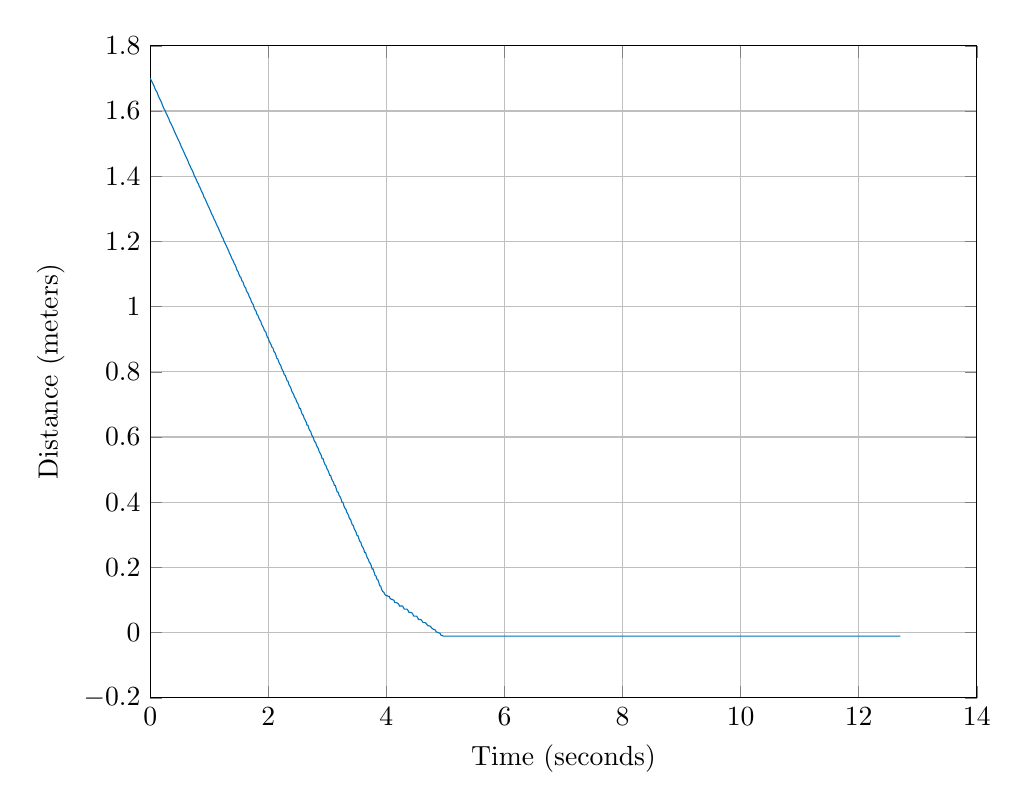
\begin{tikzpicture}

\begin{axis}[%
width=4.133in,
height=3.26in,
at={(0.693in,0.44in)},
scale only axis,
xmin=0,
xmax=14,
xmajorgrids,
xlabel={Time (seconds)},
ymin=-0.2,
ymax=1.8,
ymajorgrids,
ylabel={Distance (meters)},
axis background/.style={fill=white}
]
\addplot [color=mycolor1,solid,forget plot]
  table[row sep=crcr]{%
0	1.70085555414481\\
0.0153211270009987	1.69463180013757\\
0.0309043720009997	1.68879709871632\\
0.0469654179999996	1.68295636037074\\
0.0629747400009986	1.67712396882657\\
0.0789483189989999	1.66935225978683\\
0.0949689349989984	1.66351158618384\\
0.110946511999998	1.65913052987804\\
0.127029569999998	1.65145368146703\\
0.142841192000998	1.64366787869236\\
0.158836215	1.6378491400838\\
0.174881240999999	1.63200852472612\\
0.190889718999999	1.62617589639059\\
0.206836572999999	1.61790505727001\\
0.222930619999999	1.61110092576198\\
0.238808220999999	1.60482614507257\\
0.254836555	1.60050562666044\\
0.270782398999998	1.59271970004633\\
0.286693944999998	1.58690029329222\\
0.302928994000999	1.58056182449613\\
0.318795630999999	1.5747290488527\\
0.334774294	1.56599443328329\\
0.350862424999999	1.56164806855035\\
0.366816389999999	1.55539705697473\\
0.382793973001	1.54955664017828\\
0.398847903999999	1.54177075913353\\
0.414838353999998	1.53545343991318\\
0.430911060000999	1.52912720139101\\
0.446985636	1.52281943017435\\
0.462986320999999	1.51654287572394\\
0.478975730999999	1.51026762577778\\
0.494844794	1.50444718469753\\
0.510838454	1.49811028801192\\
0.526748222999999	1.48983911972419\\
0.544733397000998	1.48354445202002\\
0.560240241999999	1.4777043691064\\
0.575744968000999	1.47142661009154\\
0.591028805	1.4651633380271\\
0.606993363	1.45882170922588\\
0.623017703	1.45300079749809\\
0.638800810999999	1.44667602260447\\
0.65480127	1.43841673206862\\
0.670805200999999	1.43259560242902\\
0.686829447000999	1.42631038578797\\
0.702817343999999	1.42047685943771\\
0.718842830999998	1.41565770654096\\
0.734828707999999	1.40738784830211\\
0.750933603999998	1.39914380136822\\
0.766857553001	1.39525370283352\\
0.783527904999999	1.38746800957908\\
0.799015937999999	1.38119988637825\\
0.814983863999998	1.37680351499444\\
0.831076607999999	1.36859739422504\\
0.846812268000999	1.36422391071236\\
0.863121798999999	1.35596592328441\\
0.879241789999999	1.350143736628\\
0.895074896	1.34430422539696\\
0.910947661999999	1.33557736709344\\
0.926906471999999	1.33169600981242\\
0.942971558999998	1.32493566017855\\
0.960692801999999	1.31716357185394\\
0.976129404999999	1.31085832620574\\
0.991840934998998	1.30501630821809\\
1.007330869001	1.29870001227125\\
1.023366813	1.29241314180737\\
1.038714443	1.28462703328804\\
1.055000777001	1.27982714638208\\
1.070742936	1.27351424845138\\
1.086727199	1.26574201224783\\
1.102720736	1.26185180285777\\
1.118701559	1.25357318687097\\
1.134822672	1.24730129081577\\
1.150815728	1.24291934597878\\
1.166740637	1.23470993409273\\
1.182730904	1.22840576857752\\
1.198748995	1.2225638834473\\
1.21472884	1.21429895692886\\
1.230791924	1.21040907975991\\
1.246777660999	1.20217376788201\\
1.262696504001	1.19586907731025\\
1.280790890001	1.18959245492781\\
1.296234924	1.18328896592096\\
1.311775262	1.17745446828559\\
1.327122081	1.17112135202694\\
1.342965125	1.16334826699458\\
1.358951337	1.15852832942738\\
1.375230113	1.1507424005068\\
1.390967337001	1.14444922317775\\
1.406949581001	1.1401108558265\\
1.423094844001	1.13184652602298\\
1.438846464999	1.12795665700789\\
1.454882631	1.12017051197722\\
1.470830677	1.11146709844904\\
1.486850722	1.1075767376068\\
1.502962254	1.09932316495283\\
1.518704126001	1.09256863370344\\
1.536977293	1.08866930457686\\
1.552389709001	1.07894409588947\\
1.567973921	1.07652652581213\\
1.583381964	1.06828927434658\\
1.598966302	1.06051499814053\\
1.615094105	1.05809703832493\\
1.631103801001	1.04744263698718\\
1.646967822	1.04355894390835\\
1.663007271	1.0377175817525\\
1.679093971001	1.02946536766691\\
1.695000694	1.02512322553629\\
1.71094643	1.01687082121135\\
1.726929857	1.01055594372125\\
1.742945621	1.0062166745319\\
1.758919976999	0.996490984636436\\
1.775766182	0.990187192175584\\
1.790960897001	0.986288807857533\\
1.807189545	0.976110061611727\\
1.822965927	0.973217221906783\\
1.83879091	0.965431379521894\\
1.854833233	0.959162956187025\\
1.870975501001	0.955264319611449\\
1.886995991	0.945062410883226\\
1.902810963	0.940724028200181\\
1.918871199	0.934883029752935\\
1.934774394	0.92615573450781\\
1.959188541	0.922265852773963\\
1.968350355	0.914037463832562\\
1.983783174	0.905786111300837\\
1.999171808	0.903835991377178\\
2.015421209	0.893656083468396\\
2.030879719	0.888820181342798\\
2.04704812	0.882979697973254\\
2.062846322	0.875203404851157\\
2.078861530001	0.872810221017151\\
2.094830078	0.862609007581252\\
2.110966541001	0.858723193876206\\
2.126938572001	0.852429421232104\\
2.143007582001	0.841753734240257\\
2.158962332999	0.839813656209435\\
2.174984267	0.832026680449857\\
2.190833299	0.823806328524963\\
2.206798084	0.821382048118887\\
2.222776293	0.811654654114652\\
2.238865148999	0.804883622091454\\
2.255171832	0.800528152973377\\
2.270723399	0.79080050950112\\
2.288752366	0.788860512271176\\
2.304108772001	0.780155558112259\\
2.319528376001	0.772377546905012\\
2.335033735	0.770427628088341\\
2.351280362	0.759764389494186\\
2.366987543	0.755416210112212\\
2.382958772	0.749574762269771\\
2.398969766001	0.739846920502935\\
2.415029315001	0.735042424507926\\
2.430966401	0.729200714198139\\
2.447004431	0.720938737013356\\
2.463019986	0.718077398581126\\
2.478953945	0.708348974095557\\
2.494974601	0.704462298192767\\
2.510783374	0.698148686980311\\
2.526690234	0.687973980919767\\
2.542959679	0.687974054857247\\
2.558937032	0.677762347198697\\
2.574953989001	0.669072812275595\\
2.590802806	0.667123624583743\\
2.606822615	0.657394707497653\\
2.62299752	0.653036125242305\\
2.638972954	0.646747549755944\\
2.654980475	0.636536315488634\\
2.670989930001	0.636536171495944\\
2.686848293	0.625898083777606\\
2.702817292	0.620062164147794\\
2.71893371	0.616169004010627\\
2.734851242	0.605968850282572\\
2.750818641999	0.601634087509286\\
2.766839561001	0.595310247285894\\
2.782736398999	0.585580293415733\\
2.798945648	0.584673620892499\\
2.814972062	0.574943553267998\\
2.830944352	0.568636454514682\\
2.846912509999	0.564743656849049\\
2.862970925	0.554084589638591\\
2.878973651	0.550196482043489\\
2.894984925	0.544354393729595\\
2.910947204	0.533718247588318\\
2.92695255	0.533718376593124\\
2.943003850001	0.523518569179329\\
2.960741816	0.515252364936212\\
2.976132615	0.512859156974905\\
2.991652371	0.503127973752533\\
3.007147963	0.498782553390948\\
3.022692829	0.49249284921887\\
3.038772561	0.482761264344188\\
3.054964313001	0.482293447417175\\
3.070957051001	0.472082201434549\\
3.086982769	0.465795622986126\\
3.102960457	0.461902641423671\\
3.118953149	0.451713583955948\\
3.134832313999	0.451267601125166\\
3.150822913	0.441067446042416\\
3.166788944	0.431335595211034\\
3.182815153	0.430856521980807\\
3.198995646	0.420676873996759\\
3.215021338	0.416788026543761\\
3.230937252	0.410488026668262\\
3.246941334999	0.400309860812253\\
3.262925784001	0.399843410070219\\
3.278714481	0.389631739258709\\
3.296857185001	0.381843232341481\\
3.312201796	0.379452465809501\\
3.327490494001	0.369718524327037\\
3.343321856	0.365373603987694\\
3.358981424	0.359085426514212\\
3.374969341	0.348885141812172\\
3.391093039	0.348407513653567\\
3.407065301	0.338674032217837\\
3.42297486	0.330438577730302\\
3.438936382	0.328493564526312\\
3.454967627001	0.318304898857782\\
3.470829733001	0.313505806833666\\
3.486966222	0.307183860235008\\
3.503067329	0.297449061068344\\
3.518762586001	0.297449813391747\\
3.534720522001	0.287269184361894\\
3.550694821	0.279478975488576\\
3.566915645	0.277080496640759\\
3.582939347	0.266436843952904\\
3.598959108	0.262070403198659\\
3.614927145	0.256225908800227\\
3.630984359	0.246489517011821\\
3.646991123	0.246045398903351\\
3.662954073	0.235856693385205\\
3.678965026999	0.228065342532466\\
3.694945417001	0.224738330235533\\
3.711028604	0.21500274934534\\
3.726929549	0.213054876527695\\
3.743031805	0.205265660599955\\
3.759029032	0.195085786768091\\
3.774694298	0.195085879055576\\
3.792663368	0.184896068101303\\
3.807452128	0.175724924202197\\
3.822991975	0.173780499532916\\
3.838844154	0.164042428978696\\
3.854721729	0.162094550452018\\
3.870938536	0.153862690162819\\
3.886960775	0.143672815813234\\
3.903074105	0.142736556348713\\
3.918830728	0.132558310290054\\
3.934920445	0.126716161839171\\
3.959220631001	0.122819837217316\\
3.967895728	0.118926236120861\\
3.983019482001	0.115032607434564\\
3.998878442	0.11308169194714\\
4.014727699	0.11308169194714\\
4.030690212	0.11113318765288\\
4.048644835	0.110691111892349\\
4.063895993	0.104851608342663\\
4.079218256001	0.102449770450324\\
4.094860886001	0.102449770450324\\
4.110812916	0.100501266156065\\
4.126846947001	0.0995654524211425\\
4.142827512	0.0917750333840313\\
4.158828769	0.0917750333840313\\
4.174799267	0.0917750333840313\\
4.190834190001	0.0898265290897724\\
4.206841826	0.0874430574162826\\
4.222825829	0.0815957366191666\\
4.238835254	0.0815957366191666\\
4.25483403	0.0815957366191666\\
4.27075688	0.0815957366191666\\
4.286745791001	0.0777041340849127\\
4.302807803001	0.0718568132877968\\
4.318826846001	0.0718568132877968\\
4.334820006	0.0718568132877968\\
4.350735384	0.0718568132877968\\
4.366808025	0.0679652107535427\\
4.382783409001	0.062117889956427\\
4.398935942	0.061675814195896\\
4.414915264	0.061675814195896\\
4.430796007	0.0612248917909806\\
4.446968463	0.0568596129645953\\
4.463035379001	0.0505501547246889\\
4.478933236	0.0505501547246889\\
4.494939154	0.0505501547246889\\
4.511108987	0.0505501547246889\\
4.526687661	0.0466585521904348\\
4.544658824	0.0403708579598243\\
4.559529552	0.0403708579598243\\
4.574642244001	0.0403708579598243\\
4.592890462	0.038427759719829\\
4.608202513002	0.0345287249792683\\
4.623597347	0.0306319346284545\\
4.639065326	0.0306319346284545\\
4.654966276	0.0306319346284545\\
4.670958046	0.0286888363884592\\
4.686706575	0.024789801647898\\
4.7049055	0.0208930112970842\\
4.720183699001	0.0208930112970842\\
4.735563769	0.0204509355365534\\
4.751144709	0.0180341610044268\\
4.766694092	0.014135126263866\\
4.784770133	0.0117332883715262\\
4.79987471	0.00932527606534617\\
4.815404058	0.00932527606534617\\
4.830913866	0.00738217782535089\\
4.846969912	0.00153222759736549\\
4.862940042999	0.00153222759736549\\
4.878853832	-0.000413647266023665\\
4.894833184	-0.000854020699518232\\
4.91085828	-0.00279711893951351\\
4.926965226	-0.00864706916749869\\
4.942974797	-0.00864706916749869\\
4.960656134999	-0.0105929440308881\\
4.975933181	-0.0105929440308881\\
4.99115142	-0.0105929440308881\\
5.006837653	-0.0105929440308881\\
5.022691761001	-0.0105929440308881\\
5.040854695	-0.0105929440308881\\
5.055943029	-0.0105929440308881\\
5.071453869001	-0.0105929440308881\\
5.087006921002	-0.0105929440308881\\
5.102933404	-0.0105929440308881\\
5.118972762	-0.0105929440308881\\
5.134993548	-0.0105929440308881\\
5.151077136001	-0.0105929440308881\\
5.166971411	-0.0105929440308881\\
5.182970874001	-0.0105929440308881\\
5.198973048	-0.0105929440308881\\
5.214846956001	-0.0105929440308881\\
5.230784203	-0.0105929440308881\\
5.246820945001	-0.0105929440308881\\
5.262894405	-0.0105929440308881\\
5.27875867	-0.0105929440308881\\
5.294916559	-0.0105929440308881\\
5.310958153	-0.0105929440308881\\
5.326968725001	-0.0105929440308881\\
5.342934131	-0.0105929440308881\\
5.359005492	-0.0105929440308881\\
5.374937847	-0.0105929440308881\\
5.39108508	-0.0105929440308881\\
5.407008615	-0.0105929440308881\\
5.422847875	-0.0105929440308881\\
5.438904047	-0.0105929440308881\\
5.454929127	-0.0105929440308881\\
5.47102334	-0.0105929440308881\\
5.486978247	-0.0105929440308881\\
5.503098101999	-0.0105929440308881\\
5.518779343001	-0.0105929440308881\\
5.534728293	-0.0105929440308881\\
5.550934988	-0.0105929440308881\\
5.566955438	-0.0105929440308881\\
5.582851648999	-0.0105929440308881\\
5.598820543	-0.0105929440308881\\
5.614940398001	-0.0105929440308881\\
5.630948496	-0.0105929440308881\\
5.646891826	-0.0105929440308881\\
5.662927306001	-0.0105929440308881\\
5.678913077	-0.0105929440308881\\
5.694816332	-0.0105929440308881\\
5.710775228001	-0.0105929440308881\\
5.72694194	-0.0105929440308881\\
5.742936301001	-0.0105929440308881\\
5.758814721001	-0.0105929440308881\\
5.774761749	-0.0105929440308881\\
5.791050776999	-0.0105929440308881\\
5.807003524	-0.0105929440308881\\
5.822977981	-0.0105929440308881\\
5.839067994001	-0.0105929440308881\\
5.854780837	-0.0105929440308881\\
5.870943194	-0.0105929440308881\\
5.886947858	-0.0105929440308881\\
5.902936126	-0.0105929440308881\\
5.919162338	-0.0105929440308881\\
5.934932937	-0.0105929440308881\\
5.956786725001	-0.0105929440308881\\
5.968608009	-0.0105929440308881\\
5.983703935001	-0.0105929440308881\\
5.998870891999	-0.0105929440308881\\
6.014748868	-0.0105929440308881\\
6.030687781	-0.0105929440308881\\
6.048645433	-0.0105929440308881\\
6.063693096	-0.0105929440308881\\
6.079164127	-0.0105929440308881\\
6.094846887	-0.0105929440308881\\
6.110833686	-0.0105929440308881\\
6.126800014	-0.0105929440308881\\
6.14296652	-0.0105929440308881\\
6.15883025	-0.0105929440308881\\
6.174826842	-0.0105929440308881\\
6.190784445001	-0.0105929440308881\\
6.206793535	-0.0105929440308881\\
6.222857985001	-0.0105929440308881\\
6.238866022001	-0.0105929440308881\\
6.254854179	-0.0105929440308881\\
6.273249653	-0.0105929440308881\\
6.288437594	-0.0105929440308881\\
6.303792988	-0.0105929440308881\\
6.319269681	-0.0105929440308881\\
6.334962079	-0.0105929440308881\\
6.350864587	-0.0105929440308881\\
6.366798691	-0.0105929440308881\\
6.382960748	-0.0105929440308881\\
6.399011447001	-0.0105929440308881\\
6.414964765	-0.0105929440308881\\
6.430924751	-0.0105929440308881\\
6.446860091	-0.0105929440308881\\
6.462942146	-0.0105929440308881\\
6.478991216	-0.0105929440308881\\
6.49496925	-0.0105929440308881\\
6.510867163	-0.0105929440308881\\
6.526720714999	-0.0105929440308881\\
6.544727958	-0.0105929440308881\\
6.559586448	-0.0105929440308881\\
6.574636525001	-0.0105929440308881\\
6.592783784	-0.0105929440308881\\
6.607882412	-0.0105929440308881\\
6.623006737	-0.0105929440308881\\
6.638958011001	-0.0105929440308881\\
6.655038186	-0.0105929440308881\\
6.67112619	-0.0105929440308881\\
6.686898513	-0.0105929440308881\\
6.703127917	-0.0105929440308881\\
6.719050506001	-0.0105929440308881\\
6.734948944	-0.0105929440308881\\
6.750839476	-0.0105929440308881\\
6.766892404	-0.0105929440308881\\
6.782734198	-0.0105929440308881\\
6.798965824001	-0.0105929440308881\\
6.814917047	-0.0105929440308881\\
6.830870611	-0.0105929440308881\\
6.846826004001	-0.0105929440308881\\
6.863109212	-0.0105929440308881\\
6.878805751	-0.0105929440308881\\
6.894938897001	-0.0105929440308881\\
6.910925175	-0.0105929440308881\\
6.926987861	-0.0105929440308881\\
6.942861855	-0.0105929440308881\\
6.96057962	-0.0105929440308881\\
6.976000753	-0.0105929440308881\\
6.991991440001	-0.0105929440308881\\
7.007224325999	-0.0105929440308881\\
7.022692230002	-0.0105929440308881\\
7.040911492	-0.0105929440308881\\
7.056044321	-0.0105929440308881\\
7.071360082	-0.0105929440308881\\
7.086813651999	-0.0105929440308881\\
7.102768313	-0.0105929440308881\\
7.118770467	-0.0105929440308881\\
7.134837142	-0.0105929440308881\\
7.15081902	-0.0105929440308881\\
7.16680855	-0.0105929440308881\\
7.182833471001	-0.0105929440308881\\
7.198788848001	-0.0105929440308881\\
7.214793508	-0.0105929440308881\\
7.230806757	-0.0105929440308881\\
7.246776949001	-0.0105929440308881\\
7.262871517	-0.0105929440308881\\
7.278722679	-0.0105929440308881\\
7.294713542	-0.0105929440308881\\
7.312904740001	-0.0105929440308881\\
7.328473467	-0.0105929440308881\\
7.343936584	-0.0105929440308881\\
7.35923988	-0.0105929440308881\\
7.37480979	-0.0105929440308881\\
7.391055746	-0.0105929440308881\\
7.407221471	-0.0105929440308881\\
7.423093239	-0.0105929440308881\\
7.438878983	-0.0105929440308881\\
7.455044848	-0.0105929440308881\\
7.470892066	-0.0105929440308881\\
7.486852129	-0.0105929440308881\\
7.502872364001	-0.0105929440308881\\
7.51868362	-0.0105929440308881\\
7.534704538	-0.0105929440308881\\
7.550737107001	-0.0105929440308881\\
7.566736208	-0.0105929440308881\\
7.582872369001	-0.0105929440308881\\
7.598907373	-0.0105929440308881\\
7.614821898	-0.0105929440308881\\
7.630782909	-0.0105929440308881\\
7.646818056999	-0.0105929440308881\\
7.662828986	-0.0105929440308881\\
7.681256018001	-0.0105929440308881\\
7.696812272	-0.0105929440308881\\
7.712177588	-0.0105929440308881\\
7.728098508001	-0.0105929440308881\\
7.743428259	-0.0105929440308881\\
7.758871206001	-0.0105929440308881\\
7.774765784	-0.0105929440308881\\
7.790669454	-0.0105929440308881\\
7.807114715	-0.0105929440308881\\
7.822985477	-0.0105929440308881\\
7.838880277001	-0.0105929440308881\\
7.855103837	-0.0105929440308881\\
7.871271280001	-0.0105929440308881\\
7.887035966	-0.0105929440308881\\
7.902799847	-0.0105929440308881\\
7.918914640001	-0.0105929440308881\\
7.934669112	-0.0105929440308881\\
7.955672651	-0.0105929440308881\\
7.967643933001	-0.0105929440308881\\
7.982794004	-0.0105929440308881\\
7.998791846	-0.0105929440308881\\
8.014783042	-0.0105929440308881\\
8.030684751	-0.0105929440308881\\
8.048684135	-0.0105929440308881\\
8.064063139	-0.0105929440308881\\
8.079332277001	-0.0105929440308881\\
8.094850784	-0.0105929440308881\\
8.110835934	-0.0105929440308881\\
8.12688302	-0.0105929440308881\\
8.142844913	-0.0105929440308881\\
8.158775528	-0.0105929440308881\\
8.174856196	-0.0105929440308881\\
8.190831189	-0.0105929440308881\\
8.206842549	-0.0105929440308881\\
8.222846241	-0.0105929440308881\\
8.238854815	-0.0105929440308881\\
8.254845783	-0.0105929440308881\\
8.270705288	-0.0105929440308881\\
8.28685165	-0.0105929440308881\\
8.302929284	-0.0105929440308881\\
8.318857997	-0.0105929440308881\\
8.334836392	-0.0105929440308881\\
8.353108072	-0.0105929440308881\\
8.368146117001	-0.0105929440308881\\
8.383178745001	-0.0105929440308881\\
8.398900779	-0.0105929440308881\\
8.414818562	-0.0105929440308881\\
8.430930168	-0.0105929440308881\\
8.446901858	-0.0105929440308881\\
8.46282789	-0.0105929440308881\\
8.478881736	-0.0105929440308881\\
8.494968316	-0.0105929440308881\\
8.510901289001	-0.0105929440308881\\
8.526796964001	-0.0105929440308881\\
8.542971041001	-0.0105929440308881\\
8.55897953	-0.0105929440308881\\
8.574942263002	-0.0105929440308881\\
8.590960533	-0.0105929440308881\\
8.606992754	-0.0105929440308881\\
8.622959763002	-0.0105929440308881\\
8.638941897	-0.0105929440308881\\
8.654924963	-0.0105929440308881\\
8.670962888002	-0.0105929440308881\\
8.686962571	-0.0105929440308881\\
8.702840699	-0.0105929440308881\\
8.718976722	-0.0105929440308881\\
8.734953854	-0.0105929440308881\\
8.750834913	-0.0105929440308881\\
8.766865722	-0.0105929440308881\\
8.782682886001	-0.0105929440308881\\
8.798961096	-0.0105929440308881\\
8.81497433	-0.0105929440308881\\
8.830895581001	-0.0105929440308881\\
8.846812349	-0.0105929440308881\\
8.862811628	-0.0105929440308881\\
8.878955108001	-0.0105929440308881\\
8.894955167	-0.0105929440308881\\
8.910946616	-0.0105929440308881\\
8.926944756	-0.0105929440308881\\
8.942982601	-0.0105929440308881\\
8.960450635	-0.0105929440308881\\
8.97575087	-0.0105929440308881\\
8.990897325	-0.0105929440308881\\
9.007081602	-0.0105929440308881\\
9.022866022	-0.0105929440308881\\
9.038691528	-0.0105929440308881\\
9.05716137	-0.0105929440308881\\
9.072551843001	-0.0105929440308881\\
9.088020062	-0.0105929440308881\\
9.103413983001	-0.0105929440308881\\
9.118991887	-0.0105929440308881\\
9.134878458	-0.0105929440308881\\
9.150941841001	-0.0105929440308881\\
9.166967097	-0.0105929440308881\\
9.182833288	-0.0105929440308881\\
9.198812274	-0.0105929440308881\\
9.214966257	-0.0105929440308881\\
9.230959456	-0.0105929440308881\\
9.247034415	-0.0105929440308881\\
9.262924375	-0.0105929440308881\\
9.278791983	-0.0105929440308881\\
9.294702463	-0.0105929440308881\\
9.312723601	-0.0105929440308881\\
9.327682112	-0.0105929440308881\\
9.343232398	-0.0105929440308881\\
9.359020642	-0.0105929440308881\\
9.374754371	-0.0105929440308881\\
9.390689337	-0.0105929440308881\\
9.406773288	-0.0105929440308881\\
9.422734334001	-0.0105929440308881\\
9.438777058001	-0.0105929440308881\\
9.454967566	-0.0105929440308881\\
9.470841825	-0.0105929440308881\\
9.486845588	-0.0105929440308881\\
9.503115819	-0.0105929440308881\\
9.518741553001	-0.0105929440308881\\
9.534696823	-0.0105929440308881\\
9.552660767	-0.0105929440308881\\
9.567833426	-0.0105929440308881\\
9.583198738	-0.0105929440308881\\
9.598841609	-0.0105929440308881\\
9.614820283	-0.0105929440308881\\
9.630824	-0.0105929440308881\\
9.646814302	-0.0105929440308881\\
9.662814456	-0.0105929440308881\\
9.678822183	-0.0105929440308881\\
9.694944304	-0.0105929440308881\\
9.710835967	-0.0105929440308881\\
9.726860943	-0.0105929440308881\\
9.743150914001	-0.0105929440308881\\
9.759028114	-0.0105929440308881\\
9.77469119	-0.0105929440308881\\
9.790649518999	-0.0105929440308881\\
9.808704187	-0.0105929440308881\\
9.824223955	-0.0105929440308881\\
9.838916174999	-0.0105929440308881\\
9.854856189	-0.0105929440308881\\
9.870855722	-0.0105929440308881\\
9.886811195	-0.0105929440308881\\
9.90280264	-0.0105929440308881\\
9.918815849	-0.0105929440308881\\
9.934786647001	-0.0105929440308881\\
9.956866688	-0.0105929440308881\\
9.968746904	-0.0105929440308881\\
9.983825931	-0.0105929440308881\\
9.998998867	-0.0105929440308881\\
10.014839211001	-0.0105929440308881\\
10.031412443	-0.0105929440308881\\
10.046962576	-0.0105929440308881\\
10.062937381001	-0.0105929440308881\\
10.078855567001	-0.0105929440308881\\
10.094826262	-0.0105929440308881\\
10.110826952	-0.0105929440308881\\
10.12682425	-0.0105929440308881\\
10.142955105002	-0.0105929440308881\\
10.158973587	-0.0105929440308881\\
10.175026992	-0.0105929440308881\\
10.190973509	-0.0105929440308881\\
10.207097028	-0.0105929440308881\\
10.223085371	-0.0105929440308881\\
10.238835268	-0.0105929440308881\\
10.254968324001	-0.0105929440308881\\
10.273574394	-0.0105929440308881\\
10.288482038	-0.0105929440308881\\
10.303430276999	-0.0105929440308881\\
10.319033052	-0.0105929440308881\\
10.335058797	-0.0105929440308881\\
10.350989571	-0.0105929440308881\\
10.366984605002	-0.0105929440308881\\
10.382970464	-0.0105929440308881\\
10.399023296002	-0.0105929440308881\\
10.414838455	-0.0105929440308881\\
10.430930342	-0.0105929440308881\\
10.447030503	-0.0105929440308881\\
10.462931417999	-0.0105929440308881\\
10.479002242	-0.0105929440308881\\
10.494937023	-0.0105929440308881\\
10.510998101	-0.0105929440308881\\
10.527631333	-0.0105929440308881\\
10.542665711001	-0.0105929440308881\\
10.561079718001	-0.0105929440308881\\
10.576557081001	-0.0105929440308881\\
10.591992068001	-0.0105929440308881\\
10.607490454	-0.0105929440308881\\
10.623011755	-0.0105929440308881\\
10.638958172	-0.0105929440308881\\
10.655142434	-0.0105929440308881\\
10.670804785	-0.0105929440308881\\
10.686817001	-0.0105929440308881\\
10.702817009	-0.0105929440308881\\
10.718945579	-0.0105929440308881\\
10.734964996	-0.0105929440308881\\
10.750809186	-0.0105929440308881\\
10.766888677	-0.0105929440308881\\
10.78422787	-0.0105929440308881\\
10.79921292	-0.0105929440308881\\
10.814992128	-0.0105929440308881\\
10.830792145	-0.0105929440308881\\
10.846965039001	-0.0105929440308881\\
10.86296221	-0.0105929440308881\\
10.878836332	-0.0105929440308881\\
10.894844624	-0.0105929440308881\\
10.910937414001	-0.0105929440308881\\
10.926949811	-0.0105929440308881\\
10.942990076	-0.0105929440308881\\
10.958975769	-0.0105929440308881\\
10.974912939	-0.0105929440308881\\
10.99097105	-0.0105929440308881\\
11.006973515	-0.0105929440308881\\
11.022851227	-0.0105929440308881\\
11.038725357001	-0.0105929440308881\\
11.054963892	-0.0105929440308881\\
11.070965297001	-0.0105929440308881\\
11.086945496	-0.0105929440308881\\
11.103067726999	-0.0105929440308881\\
11.119086744001	-0.0105929440308881\\
11.134882400001	-0.0105929440308881\\
11.150850141001	-0.0105929440308881\\
11.166841696	-0.0105929440308881\\
11.182820297	-0.0105929440308881\\
11.198938659	-0.0105929440308881\\
11.214910459001	-0.0105929440308881\\
11.230881551	-0.0105929440308881\\
11.246937372999	-0.0105929440308881\\
11.262971249001	-0.0105929440308881\\
11.280549348	-0.0105929440308881\\
11.295979796	-0.0105929440308881\\
11.311682813	-0.0105929440308881\\
11.326930954	-0.0105929440308881\\
11.34287013	-0.0105929440308881\\
11.358831582	-0.0105929440308881\\
11.374831701	-0.0105929440308881\\
11.390912228	-0.0105929440308881\\
11.406930383	-0.0105929440308881\\
11.423089507	-0.0105929440308881\\
11.438877446	-0.0105929440308881\\
11.454841749	-0.0105929440308881\\
11.470830662999	-0.0105929440308881\\
11.48694219	-0.0105929440308881\\
11.502948819	-0.0105929440308881\\
11.518868651	-0.0105929440308881\\
11.53487757	-0.0105929440308881\\
11.550941604	-0.0105929440308881\\
11.566978587	-0.0105929440308881\\
11.582846983	-0.0105929440308881\\
11.598958825	-0.0105929440308881\\
11.614902752	-0.0105929440308881\\
11.630948365	-0.0105929440308881\\
11.646937985	-0.0105929440308881\\
11.662967075001	-0.0105929440308881\\
11.678935748	-0.0105929440308881\\
11.69484869	-0.0105929440308881\\
11.710832938001	-0.0105929440308881\\
11.726835017	-0.0105929440308881\\
11.742824412	-0.0105929440308881\\
11.758938299	-0.0105929440308881\\
11.774735111	-0.0105929440308881\\
11.790717382	-0.0105929440308881\\
11.806909669	-0.0105929440308881\\
11.822959032001	-0.0105929440308881\\
11.838840127	-0.0105929440308881\\
11.854841153	-0.0105929440308881\\
11.870962743	-0.0105929440308881\\
11.886929902001	-0.0105929440308881\\
11.902987607001	-0.0105929440308881\\
11.918999904	-0.0105929440308881\\
11.935001852	-0.0105929440308881\\
11.959463209	-0.0105929440308881\\
11.968159398	-0.0105929440308881\\
11.983454369001	-0.0105929440308881\\
11.998846231	-0.0105929440308881\\
12.014882397001	-0.0105929440308881\\
12.031234589	-0.0105929440308881\\
12.046716988	-0.0105929440308881\\
12.062839969	-0.0105929440308881\\
12.078872388002	-0.0105929440308881\\
12.094856235	-0.0105929440308881\\
12.110819463	-0.0105929440308881\\
12.126893315	-0.0105929440308881\\
12.14285204	-0.0105929440308881\\
12.1588305	-0.0105929440308881\\
12.174852885	-0.0105929440308881\\
12.190802236	-0.0105929440308881\\
12.206841252	-0.0105929440308881\\
12.222861166	-0.0105929440308881\\
12.238866177	-0.0105929440308881\\
12.25482394	-0.0105929440308881\\
12.270860653	-0.0105929440308881\\
12.286850603	-0.0105929440308881\\
12.302834581001	-0.0105929440308881\\
12.318817727	-0.0105929440308881\\
12.334853848	-0.0105929440308881\\
12.350838091001	-0.0105929440308881\\
12.366815088	-0.0105929440308881\\
12.382719403	-0.0105929440308881\\
12.398763836001	-0.0105929440308881\\
12.41480287	-0.0105929440308881\\
12.430721994001	-0.0105929440308881\\
12.448956208	-0.0105929440308881\\
12.464302795	-0.0105929440308881\\
12.479647722	-0.0105929440308881\\
12.495004294	-0.0105929440308881\\
12.511023987	-0.0105929440308881\\
12.527220473001	-0.0105929440308881\\
12.542944063999	-0.0105929440308881\\
12.558987226	-0.0105929440308881\\
12.574883706	-0.0105929440308881\\
12.590816678001	-0.0105929440308881\\
12.607111084	-0.0105929440308881\\
12.62294408	-0.0105929440308881\\
12.638970744001	-0.0105929440308881\\
12.655248056	-0.0105929440308881\\
12.671038119001	-0.0105929440308881\\
12.687070697	-0.0105929440308881\\
12.70297508	-0.0105929440308881\\
};
\end{axis}
\end{tikzpicture}%
}
      \caption{The error in displacement of the robot over time for
        $(K_{\Psi}^R, K_{\omega}^T) \equiv (0.5 K_{\Psi, max}^R, 0.5 K_{\omega, max}^T)$}
      \label{fig:19_11_distance}
    \end{figure}
  \end{minipage}
  \hfill
  \begin{minipage}{0.45\linewidth}
    \begin{figure}[H]
      \scalebox{0.6}{% This file was created by matlab2tikz.
%
%The latest updates can be retrieved from
%  http://www.mathworks.com/matlabcentral/fileexchange/22022-matlab2tikz-matlab2tikz
%where you can also make suggestions and rate matlab2tikz.
%
\definecolor{mycolor1}{rgb}{0.00000,0.44700,0.74100}%
%
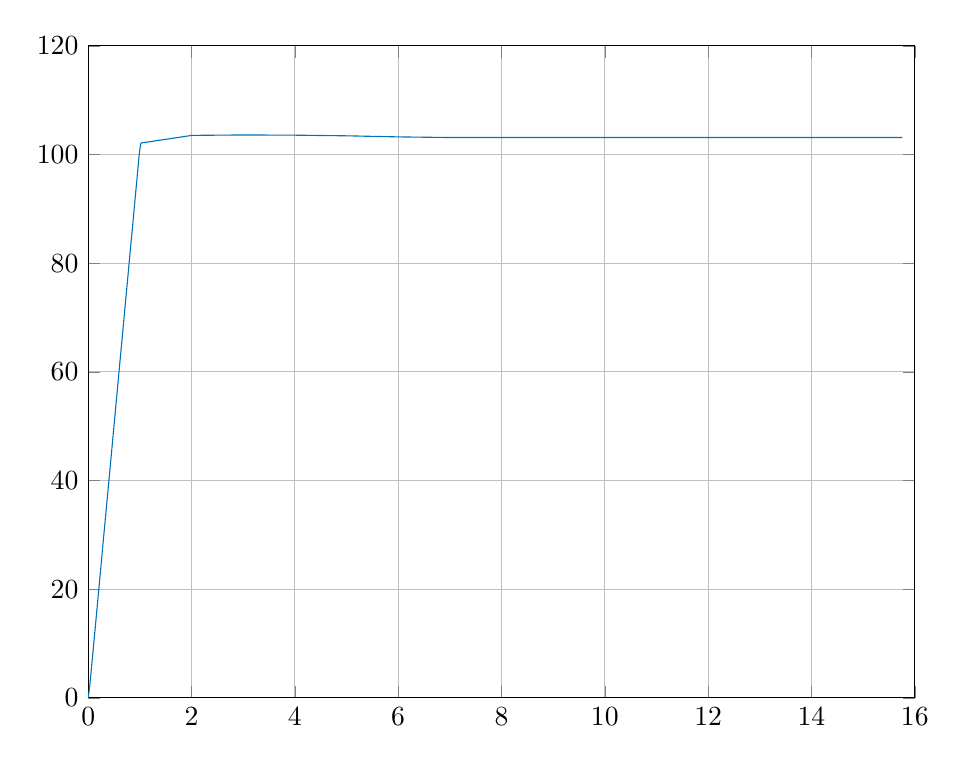
\begin{tikzpicture}

\begin{axis}[%
width=4.133in,
height=3.26in,
at={(0.693in,0.44in)},
scale only axis,
xmin=0,
xmax=16,
xmajorgrids,
ymin=0,
ymax=120,
ymajorgrids,
axis background/.style={fill=white}
]
\addplot [color=mycolor1,solid,forget plot]
  table[row sep=crcr]{%
0	0\\
0.0176569919999996	1.236\\
0.0329493709999993	2.476\\
0.0483888879999993	3.982\\
0.0640940889999997	5.552\\
0.0798458949989993	7.15\\
0.0958887509999992	8.776\\
0.111983863000999	10.406\\
0.127921078	12.046\\
0.143937094	13.674\\
0.159972982	15.324\\
0.175995181001999	16.956\\
0.191998524999999	18.582\\
0.207984587001	20.22\\
0.224022642	21.862\\
0.240222648999999	23.494\\
0.255975674001	25.132\\
0.272023266	26.84\\
0.28799259	28.51\\
0.303978898999999	30.12\\
0.319895037001	31.726\\
0.336037301999999	33.338\\
0.352051528	34.962\\
0.367968793	36.602\\
0.383873009001	38.244\\
0.399862312999999	39.864\\
0.416022466000999	41.506\\
0.432019031999999	43.154\\
0.448131865999999	44.766\\
0.464108878	46.416\\
0.480017946	48.044\\
0.495980695999999	49.696\\
0.512107225999999	51.346\\
0.528123782999999	53.02\\
0.544085962001	54.632\\
0.560119726999999	56.26\\
0.575859410999999	57.878\\
0.592148155	59.484\\
0.608002543	61.192\\
0.624022842999999	62.8\\
0.640116214001999	64.434\\
0.656129908999999	66.064\\
0.672144375999999	67.698\\
0.688173236	69.31\\
0.704075804000999	71.034\\
0.719948993999	72.636\\
0.735902495001	74.252\\
0.752065337001001	75.872\\
0.768125969	77.5\\
0.784121853000999	79.134\\
0.800171049	80.836\\
0.815850642	82.454\\
0.831850273999999	84.068\\
0.849983964001999	85.742\\
0.865510083	87.426\\
0.881092908999999	89.042\\
0.896435076	90.652\\
0.911997679	92.26\\
0.927939124000999	93.862\\
0.943900099999999	95.49\\
0.959962982	97.13\\
0.976019297999999	98.758\\
0.991988354999999	100.38\\
1.012854596001	101.768\\
1.024756646001	102.114\\
1.040019611	102.132\\
1.056009953001	102.156\\
1.071876429	102.18\\
1.087908785999	102.2\\
1.104012500999	102.222\\
1.119895645	102.246\\
1.138221575001	102.272\\
1.153239963	102.294\\
1.168241496	102.314\\
1.183957946	102.336\\
1.200037747	102.36\\
1.21612978	102.384\\
1.232136003	102.408\\
1.248014692	102.428\\
1.263995738	102.45\\
1.279987829	102.474\\
1.296001795	102.498\\
1.312014753	102.522\\
1.327903034	102.542\\
1.344139308001	102.566\\
1.360180451	102.588\\
1.376046951	102.612\\
1.392069979	102.636\\
1.408125993999	102.656\\
1.424002318001	102.68\\
1.44001917	102.702\\
1.45601478	102.726\\
1.471984831	102.75\\
1.487998065001	102.772\\
1.503985741	102.794\\
1.520101146	102.816\\
1.536048301001	102.84\\
1.552229580001	102.864\\
1.568081369	102.888\\
1.583848599	102.908\\
1.601812136001	102.932\\
1.616659084001	102.956\\
1.631999078001	102.978\\
1.64799345	103.002\\
1.663992071	103.024\\
1.680104149	103.044\\
1.695972259001	103.07\\
1.712104698001	103.092\\
1.728148175	103.116\\
1.744128901	103.138\\
1.760143809	103.162\\
1.776073809	103.182\\
1.792004756	103.206\\
1.807993174	103.23\\
1.823948729001	103.25\\
1.839894647	103.272\\
1.856088458	103.296\\
1.872161898	103.32\\
1.888054448	103.344\\
1.904106139	103.364\\
1.920131741	103.388\\
1.936119843	103.412\\
1.952172406	103.434\\
1.968225336	103.458\\
1.98413279	103.48\\
2.000128369	103.502\\
2.017452882	103.516\\
2.032446061	103.518\\
2.047875513	103.518\\
2.06600351	103.518\\
2.080914502001	103.52\\
2.095930835001	103.522\\
2.111988129001	103.522\\
2.127986805	103.524\\
2.143954752	103.526\\
2.160004057	103.526\\
2.175998709001	103.528\\
2.192023644999	103.53\\
2.208107203	103.53\\
2.224123459001	103.532\\
2.24022796	103.534\\
2.256002237	103.534\\
2.271972199	103.534\\
2.288150769	103.538\\
2.304156243999	103.538\\
2.319861292	103.538\\
2.337960481	103.542\\
2.352805525001	103.542\\
2.367983794001	103.542\\
2.383994642	103.544\\
2.399981156	103.546\\
2.418295247	103.546\\
2.433350862	103.548\\
2.448501446	103.55\\
2.464074613999	103.55\\
2.480054312	103.552\\
2.495913975	103.554\\
2.511954783999	103.554\\
2.527945517	103.556\\
2.544035074	103.558\\
2.560071536	103.558\\
2.576054206	103.56\\
2.592017366	103.562\\
2.607987462	103.562\\
2.624127293	103.562\\
2.639906073	103.566\\
2.656088473001	103.566\\
2.672128708	103.566\\
2.688122867001	103.568\\
2.704055790999	103.57\\
2.720109552	103.57\\
2.736132303	103.572\\
2.752055242001	103.574\\
2.768000863	103.574\\
2.784012373	103.576\\
2.800107231999	103.578\\
2.816064094	103.578\\
2.831929742001	103.58\\
2.847829863	103.582\\
2.865948319	103.582\\
2.881293705	103.584\\
2.896822617001	103.586\\
2.912293753	103.586\\
2.928141126	103.586\\
2.944129975	103.59\\
2.960105376	103.59\\
2.976130227	103.59\\
2.992155335	103.592\\
3.014058361999	103.594\\
3.026151745	103.588\\
3.041511649	103.59\\
3.057165543	103.592\\
3.072486670001	103.588\\
3.088069915001	103.588\\
3.104130961	103.59\\
3.120140283001	103.586\\
3.136113861999	103.586\\
3.152134477999	103.588\\
3.168112055	103.584\\
3.184195113	103.584\\
3.200006735001	103.586\\
3.216001758	103.584\\
3.232046784	103.58\\
3.248055262	103.584\\
3.264002116	103.584\\
3.280096163	103.578\\
3.295973764	103.582\\
3.312002098	103.582\\
3.327947942	103.576\\
3.343859488	103.578\\
3.360094537001	103.58\\
3.375961174	103.576\\
3.391939837	103.576\\
3.408027968	103.578\\
3.423981933	103.574\\
3.439959516001	103.574\\
3.456013447	103.576\\
3.472003897	103.572\\
3.488076603001	103.572\\
3.504151179	103.574\\
3.520151864	103.57\\
3.536141274	103.57\\
3.552010337	103.572\\
3.568003997	103.572\\
3.583913766	103.568\\
3.601898940001	103.57\\
3.617405785	103.57\\
3.632910511001	103.564\\
3.648194348	103.566\\
3.664158906	103.568\\
3.680183246	103.562\\
3.695966354	103.564\\
3.711966813	103.566\\
3.727970744	103.562\\
3.743994990001	103.562\\
3.759982887	103.564\\
3.776008374	103.56\\
3.791994251	103.56\\
3.808099147	103.562\\
3.824023096001	103.558\\
3.840693448	103.558\\
3.856181481	103.56\\
3.872149407	103.558\\
3.888242151	103.556\\
3.903977811001	103.558\\
3.920287342	103.558\\
3.936407333	103.552\\
3.952240439	103.556\\
3.968113205	103.556\\
3.984072015	103.55\\
4.000137102	103.552\\
4.017858345	103.552\\
4.033294948	103.546\\
4.049006477999	103.548\\
4.064496412001	103.548\\
4.080532356	103.542\\
4.095879986	103.542\\
4.112166320001	103.542\\
4.127908479	103.536\\
4.143892742	103.536\\
4.159886279	103.536\\
4.175867102	103.53\\
4.191988215	103.53\\
4.207981271	103.53\\
4.22390618	103.526\\
4.239896447	103.522\\
4.255914538	103.524\\
4.271894383	103.522\\
4.287957467	103.516\\
4.303943203999	103.518\\
4.319862047001	103.516\\
4.337956433001	103.51\\
4.353400467	103.512\\
4.368940805	103.512\\
4.384287624	103.506\\
4.400130668	103.506\\
4.41611688	103.506\\
4.432395656	103.5\\
4.448132880001	103.5\\
4.464115124001	103.5\\
4.480260387001	103.494\\
4.496012007999	103.494\\
4.512048174	103.494\\
4.52799622	103.49\\
4.544016265	103.488\\
4.560127797	103.488\\
4.575869669001	103.486\\
4.594142836	103.48\\
4.609555252001	103.482\\
4.625139464	103.48\\
4.640547507	103.474\\
4.656131845	103.476\\
4.672259648	103.476\\
4.688269344001	103.47\\
4.704133365	103.47\\
4.720172814	103.47\\
4.736259514001	103.464\\
4.752166237	103.464\\
4.768111973	103.464\\
4.7840954	103.458\\
4.800111164	103.458\\
4.816085519999	103.458\\
4.832931725	103.452\\
4.848126440001	103.452\\
4.864355088	103.452\\
4.88013147	103.45\\
4.895956453	103.444\\
4.911998776	103.446\\
4.928141044001	103.444\\
4.944161534	103.438\\
4.959976506	103.44\\
4.976036742	103.44\\
4.991939937	103.434\\
5.016354084	103.434\\
5.025515898	103.434\\
5.040948717	103.426\\
5.056337351	103.424\\
5.072586752	103.424\\
5.088045262	103.416\\
5.104213663	103.414\\
5.120011865	103.414\\
5.136027073001	103.408\\
5.151995621	103.404\\
5.168132084001	103.404\\
5.184104115001	103.4\\
5.200173125001	103.394\\
5.216127875999	103.394\\
5.23214981	103.392\\
5.247998842	103.384\\
5.263963627	103.384\\
5.279941836	103.382\\
5.296030691999	103.374\\
5.312337375	103.374\\
5.327888942	103.374\\
5.345917909	103.364\\
5.361274315001	103.364\\
5.376693919001	103.364\\
5.392199278	103.356\\
5.408445905	103.354\\
5.424153086	103.354\\
5.440124315	103.348\\
5.456135309001	103.344\\
5.472194858001	103.344\\
5.488131944	103.338\\
5.504169974	103.334\\
5.520185529	103.334\\
5.536119488	103.332\\
5.552140144	103.324\\
5.567948917	103.324\\
5.583855777	103.322\\
5.600125222	103.314\\
5.616102575	103.314\\
5.632119532001	103.314\\
5.647968349	103.304\\
5.663988158	103.304\\
5.680163063	103.304\\
5.696138497	103.296\\
5.712146018	103.294\\
5.728155473001	103.294\\
5.744013836	103.286\\
5.759982835	103.284\\
5.776099253	103.284\\
5.792016785	103.278\\
5.807984184999	103.274\\
5.824005104001	103.274\\
5.839901941999	103.27\\
5.856111191	103.264\\
5.872137605	103.264\\
5.888109895	103.262\\
5.904078052999	103.254\\
5.920136468	103.254\\
5.936139194	103.252\\
5.952150468	103.244\\
5.968112747	103.244\\
5.984118093	103.244\\
6.000169393001	103.236\\
6.017907359	103.234\\
6.033298158	103.234\\
6.048817914	103.23\\
6.064313506	103.228\\
6.079858372	103.228\\
6.095938104	103.224\\
6.112129856001	103.222\\
6.128122594001	103.222\\
6.144148312	103.218\\
6.160126	103.216\\
6.176118692	103.216\\
6.191997856999	103.216\\
6.207988456	103.21\\
6.223954487	103.21\\
6.239980696	103.21\\
6.256161189	103.204\\
6.272186881	103.204\\
6.288102795	103.204\\
6.304106877999	103.198\\
6.320091327001	103.198\\
6.335880024	103.198\\
6.354022728001	103.192\\
6.369367339	103.192\\
6.384656037001	103.192\\
6.400487399	103.188\\
6.416146967	103.186\\
6.432134884	103.186\\
6.448258582	103.182\\
6.464230844	103.18\\
6.480140403	103.18\\
6.496101925	103.176\\
6.512133170001	103.174\\
6.527995276001	103.174\\
6.544131765	103.174\\
6.560232872	103.168\\
6.575928129001	103.168\\
6.591886065001	103.168\\
6.607860364	103.162\\
6.624081188	103.162\\
6.64010489	103.162\\
6.656124651	103.158\\
6.672092688	103.156\\
6.688149902	103.156\\
6.704156666	103.152\\
6.720119616	103.15\\
6.736130569999	103.15\\
6.752110960001	103.146\\
6.768194147	103.144\\
6.784095092	103.144\\
6.800197348	103.14\\
6.816194575	103.138\\
6.831859841	103.138\\
6.849828911	103.138\\
6.864617671	103.132\\
6.880157518	103.132\\
6.896009697	103.132\\
6.911887272	103.126\\
6.928104079	103.126\\
6.944126318	103.126\\
6.960239648	103.12\\
6.975996271	103.12\\
6.992085988	103.12\\
7.016386174001	103.116\\
7.025061271	103.116\\
7.040185025001	103.116\\
7.056043985	103.116\\
7.071893242	103.116\\
7.087855755	103.116\\
7.105810378	103.116\\
7.121061536	103.116\\
7.136383799001	103.116\\
7.152026429001	103.116\\
7.167978459	103.116\\
7.184012490001	103.116\\
7.199993055	103.116\\
7.215994312	103.116\\
7.23196481	103.116\\
7.247999733001	103.116\\
7.264007369	103.116\\
7.279991372	103.116\\
7.296000797	103.116\\
7.311999573	103.116\\
7.327922423	103.116\\
7.343911334001	103.116\\
7.359973346001	103.116\\
7.375992389001	103.116\\
7.391985549	103.116\\
7.407900927	103.116\\
7.423973568	103.116\\
7.439948952001	103.116\\
7.456101485	103.116\\
7.472080807	103.116\\
7.48796155	103.116\\
7.504134006	103.116\\
7.520200922001	103.116\\
7.536098779	103.116\\
7.552104697	103.116\\
7.56827453	103.116\\
7.583853204	103.116\\
7.601824367	103.116\\
7.616695095	103.116\\
7.631807787001	103.116\\
7.650056005	103.116\\
7.665368056002	103.116\\
7.68076289	103.116\\
7.696230869	103.116\\
7.712131819	103.116\\
7.728123589	103.116\\
7.743872118	103.116\\
7.762071043	103.116\\
7.777349242001	103.116\\
7.792729312	103.116\\
7.808310252	103.116\\
7.823859635	103.116\\
7.841935676	103.116\\
7.857040253	103.116\\
7.872569601	103.116\\
7.888079409	103.116\\
7.904135455	103.116\\
7.920105585999	103.116\\
7.936019375	103.116\\
7.951998727	103.116\\
7.968023823	103.116\\
7.984130769	103.116\\
8.00014034	103.116\\
8.017821677999	103.116\\
8.033098724	103.116\\
8.048316963	103.116\\
8.064003196	103.116\\
8.079857304001	103.116\\
8.098020238	103.116\\
8.113108572	103.116\\
8.128619412001	103.116\\
8.144172464002	103.116\\
8.160098947	103.116\\
8.176138305	103.116\\
8.192159091	103.116\\
8.208242679001	103.116\\
8.224136954	103.116\\
8.240136417001	103.116\\
8.256138591	103.116\\
8.272012499001	103.116\\
8.287949746	103.116\\
8.303986488001	103.116\\
8.320059948	103.116\\
8.335924213	103.116\\
8.352082102	103.116\\
8.368123696	103.116\\
8.384134268001	103.116\\
8.400099674	103.116\\
8.416171035	103.116\\
8.43210339	103.116\\
8.448250623	103.116\\
8.464174158	103.116\\
8.480013418	103.116\\
8.49606959	103.116\\
8.51209467	103.116\\
8.528188883	103.116\\
8.54414379	103.116\\
8.560263644999	103.116\\
8.575944886001	103.116\\
8.591893836	103.116\\
8.608100531	103.116\\
8.624120981	103.116\\
8.640017191999	103.116\\
8.655986086	103.116\\
8.672105941001	103.116\\
8.688114039	103.116\\
8.704057369	103.116\\
8.720092849001	103.116\\
8.73607862	103.116\\
8.751981875	103.116\\
8.767940771001	103.116\\
8.784107483	103.116\\
8.800101844001	103.116\\
8.815980264001	103.116\\
8.831927292	103.116\\
8.848216319999	103.116\\
8.864169067	103.116\\
8.880143524	103.116\\
8.896233537001	103.116\\
8.91194638	103.116\\
8.928108737	103.116\\
8.944113401	103.116\\
8.960101669	103.116\\
8.976327881	103.116\\
8.99209848	103.116\\
9.013952268001	103.116\\
9.025773552	103.116\\
9.040869478001	103.116\\
9.056036434999	103.116\\
9.071914411	103.116\\
9.087853324	103.116\\
9.105810976	103.116\\
9.120858639	103.116\\
9.13632967	103.116\\
9.15201243	103.116\\
9.167999229	103.116\\
9.183965557	103.116\\
9.200132063	103.116\\
9.215995793	103.116\\
9.231992385	103.116\\
9.247949988001	103.116\\
9.263959078	103.116\\
9.280023528001	103.116\\
9.296031565001	103.116\\
9.312019722	103.116\\
9.330415196	103.116\\
9.345603137	103.116\\
9.360958531	103.116\\
9.376435224	103.116\\
9.392127622	103.116\\
9.40803013	103.116\\
9.423964234	103.116\\
9.440126291	103.116\\
9.456176990001	103.116\\
9.472130308	103.116\\
9.488090294	103.116\\
9.504025634	103.116\\
9.520107689	103.116\\
9.536156759	103.116\\
9.552134793	103.116\\
9.568032706	103.116\\
9.583886257999	103.116\\
9.601893501	103.116\\
9.616751991	103.116\\
9.631802068001	103.116\\
9.649949327	103.116\\
9.665047955	103.116\\
9.68017228	103.116\\
9.696123554001	103.116\\
9.712203729	103.116\\
9.728291733	103.116\\
9.744064056	103.116\\
9.76029346	103.116\\
9.776216049001	103.116\\
9.792114487	103.116\\
9.808005019	103.116\\
9.824057947	103.116\\
9.839899741	103.116\\
9.856131367001	103.116\\
9.87208259	103.116\\
9.888036154	103.116\\
9.903991547001	103.116\\
9.920274755	103.116\\
9.935971294	103.116\\
9.952104440001	103.116\\
9.968090718	103.116\\
9.984153404	103.116\\
10.000027398	103.116\\
10.017745163	103.116\\
10.033166296	103.116\\
10.049156983001	103.116\\
10.064389868999	103.116\\
10.079857773002	103.116\\
10.098077035	103.116\\
10.113209864	103.116\\
10.128525625	103.116\\
10.143979194999	103.116\\
10.159933856	103.116\\
10.17593601	103.116\\
10.192002685	103.116\\
10.207984563	103.116\\
10.223974093	103.116\\
10.239999014001	103.116\\
10.255954391001	103.116\\
10.271959051	103.116\\
10.2879723	103.116\\
10.303942492001	103.116\\
10.32003706	103.116\\
10.335888222	103.116\\
10.351879085	103.116\\
10.370070283001	103.116\\
10.38563901	103.116\\
10.401102127	103.116\\
10.416405423	103.116\\
10.431975333	103.116\\
10.448221289	103.116\\
10.464387014	103.116\\
10.480258782	103.116\\
10.496044526	103.116\\
10.512210391	103.116\\
10.528057609	103.116\\
10.544017672	103.116\\
10.560037907001	103.116\\
10.575849163	103.116\\
10.591870081	103.116\\
10.607902650001	103.116\\
10.623901751	103.116\\
10.640037912001	103.116\\
10.656072916	103.116\\
10.671987441	103.116\\
10.687948452	103.116\\
10.703983599999	103.116\\
10.719994529	103.116\\
10.738421561001	103.116\\
10.753977815	103.116\\
10.769343131	103.116\\
10.785264051001	103.116\\
10.800593802	103.116\\
10.816036749001	103.116\\
10.831931327	103.116\\
10.847834997	103.116\\
10.864280258	103.116\\
10.88015102	103.116\\
10.896045820001	103.116\\
10.91226938	103.116\\
10.928436823001	103.116\\
10.944201509	103.116\\
10.95996539	103.116\\
10.976080183001	103.116\\
10.991834655	103.116\\
11.012838194	103.116\\
11.024809476001	103.116\\
11.039959547	103.116\\
11.055957389	103.116\\
11.071948585	103.116\\
11.087850294	103.116\\
11.105849678	103.116\\
11.121228682	103.116\\
11.136497820001	103.116\\
11.152016327	103.116\\
11.168001477	103.116\\
11.184048563	103.116\\
11.200010456	103.116\\
11.215941071	103.116\\
11.232021739	103.116\\
11.247996732	103.116\\
11.264008092	103.116\\
11.280011784	103.116\\
11.296020358	103.116\\
11.312011326	103.116\\
11.327870831	103.116\\
11.344017193	103.116\\
11.360094827	103.116\\
11.37602354	103.116\\
11.392001935	103.116\\
11.410273615	103.116\\
11.425311660001	103.116\\
11.440344288001	103.116\\
11.456066322	103.116\\
11.471984105	103.116\\
11.488095711	103.116\\
11.504067401	103.116\\
11.519993433	103.116\\
11.536047279	103.116\\
11.552133859	103.116\\
11.568066832001	103.116\\
11.583962507001	103.116\\
11.600136584001	103.116\\
11.616145073	103.116\\
11.632107806002	103.116\\
11.648126076	103.116\\
11.664158297	103.116\\
11.680125306002	103.116\\
11.69610744	103.116\\
11.712090506	103.116\\
11.728128431002	103.116\\
11.744128114	103.116\\
11.760006242	103.116\\
11.776142265	103.116\\
11.792119397	103.116\\
11.808000456	103.116\\
11.824031265	103.116\\
11.839848429001	103.116\\
11.856126639	103.116\\
11.872139873	103.116\\
11.888061124001	103.116\\
11.903977892	103.116\\
11.919977171	103.116\\
11.936120651001	103.116\\
11.95212071	103.116\\
11.968112159	103.116\\
11.984110299	103.116\\
12.000148144	103.116\\
12.017616178	103.116\\
12.032916413	103.116\\
12.048062868	103.116\\
12.064247145	103.116\\
12.080031565	103.116\\
12.095857071	103.116\\
12.114326913	103.116\\
12.129717386001	103.116\\
12.145185605	103.116\\
12.160579526001	103.116\\
12.17615743	103.116\\
12.192044001	103.116\\
12.208107384001	103.116\\
12.22413264	103.116\\
12.239998831	103.116\\
12.255977817	103.116\\
12.2721318	103.116\\
12.288124999	103.116\\
12.304199958	103.116\\
12.320089918	103.116\\
12.335957526	103.116\\
12.351868006	103.116\\
12.369889144	103.116\\
12.384847655	103.116\\
12.400397941	103.116\\
12.416186185	103.116\\
12.431919914	103.116\\
12.44785488	103.116\\
12.463938831	103.116\\
12.479899877001	103.116\\
12.495942601001	103.116\\
12.512133109	103.116\\
12.528007368	103.116\\
12.544011131	103.116\\
12.560281362	103.116\\
12.575907096001	103.116\\
12.591862366	103.116\\
12.60982631	103.116\\
12.624998969	103.116\\
12.640364281	103.116\\
12.656007152	103.116\\
12.671985826	103.116\\
12.687989543	103.116\\
12.703979845	103.116\\
12.719979999	103.116\\
12.735987726	103.116\\
12.752109847	103.116\\
12.76800151	103.116\\
12.784026486	103.116\\
12.800316457001	103.116\\
12.816193657	103.116\\
12.831856733	103.116\\
12.847815061999	103.116\\
12.86586973	103.116\\
12.881389498	103.116\\
12.896081717999	103.116\\
12.912021732	103.116\\
12.928021265	103.116\\
12.943976738	103.116\\
12.959968183	103.116\\
12.975981392	103.116\\
12.991952190001	103.116\\
13.014032231	103.116\\
13.025912447	103.116\\
13.040991474	103.116\\
13.05616441	103.116\\
13.072004754001	103.116\\
13.088577986	103.116\\
13.104128119	103.116\\
13.120102924001	103.116\\
13.136021110001	103.116\\
13.151991805	103.116\\
13.167992495	103.116\\
13.183989793	103.116\\
13.200120648002	103.116\\
13.21613913	103.116\\
13.232192535	103.116\\
13.248139052	103.116\\
13.264262571	103.116\\
13.280250914	103.116\\
13.296000811	103.116\\
13.312133867001	103.116\\
13.330739937	103.116\\
13.345647581	103.116\\
13.360595819999	103.116\\
13.376198595	103.116\\
13.39222434	103.116\\
13.408155114	103.116\\
13.424150148002	103.116\\
13.440136007	103.116\\
13.456188839002	103.116\\
13.472003998	103.116\\
13.488095885	103.116\\
13.504196046	103.116\\
13.520096960999	103.116\\
13.536167785	103.116\\
13.552102566	103.116\\
13.568163644	103.116\\
13.584796876	103.116\\
13.599831254001	103.116\\
13.618245261001	103.116\\
13.633722624001	103.116\\
13.649157611001	103.116\\
13.664655997	103.116\\
13.680177298	103.116\\
13.696123715	103.116\\
13.712307977	103.116\\
13.727970328	103.116\\
13.743982544	103.116\\
13.759982552	103.116\\
13.776111122	103.116\\
13.792130539	103.116\\
13.807974729	103.116\\
13.82405422	103.116\\
13.841393413	103.116\\
13.856378463	103.116\\
13.872157671	103.116\\
13.887957688	103.116\\
13.904130582001	103.116\\
13.920127753	103.116\\
13.936001875	103.116\\
13.952010167	103.116\\
13.968102957001	103.116\\
13.984115354	103.116\\
14.000155619	103.116\\
14.016141312	103.116\\
14.032078482	103.116\\
14.048136593	103.116\\
14.064139058	103.116\\
14.08001677	103.116\\
14.095890900001	103.116\\
14.112129435	103.116\\
14.128130840001	103.116\\
14.144111039	103.116\\
14.160233269999	103.116\\
14.176252287001	103.116\\
14.192047943001	103.116\\
14.208015684001	103.116\\
14.224007239	103.116\\
14.23998584	103.116\\
14.256104202	103.116\\
14.272076002001	103.116\\
14.288047094	103.116\\
14.304102915999	103.116\\
14.320136792001	103.116\\
14.337714891	103.116\\
14.353145339	103.116\\
14.368848356	103.116\\
14.384096497	103.116\\
14.400035673	103.116\\
14.415997125	103.116\\
14.431997244	103.116\\
14.448077771	103.116\\
14.464095926	103.116\\
14.48025505	103.116\\
14.496042989	103.116\\
14.512007292	103.116\\
14.527996205999	103.116\\
14.544107733	103.116\\
14.560114362	103.116\\
14.576034194	103.116\\
14.592043113	103.116\\
14.608107147	103.116\\
14.62414413	103.116\\
14.640012526	103.116\\
14.656124368	103.116\\
14.672068295	103.116\\
14.688113908	103.116\\
14.704103528	103.116\\
14.720132618001	103.116\\
14.736101291	103.116\\
14.752014233	103.116\\
14.767998481001	103.116\\
14.78400056	103.116\\
14.799989955	103.116\\
14.816103842	103.116\\
14.831900654	103.116\\
14.847882925	103.116\\
14.864075212	103.116\\
14.880124575001	103.116\\
14.89600567	103.116\\
14.912006696	103.116\\
14.928128286	103.116\\
14.944095445001	103.116\\
14.960153150001	103.116\\
14.976165447	103.116\\
14.992167395	103.116\\
15.016628752	103.116\\
15.025324941	103.116\\
15.040619912001	103.116\\
15.056011774	103.116\\
15.072047940001	103.116\\
15.088400132	103.116\\
15.103882531	103.116\\
15.120005512	103.116\\
15.136037931002	103.116\\
15.152021778	103.116\\
15.167985006	103.116\\
15.184058858	103.116\\
15.200017583	103.116\\
15.215996043	103.116\\
15.232018428	103.116\\
15.247967779	103.116\\
15.264006795	103.116\\
15.280026709	103.116\\
15.29603172	103.116\\
15.311989483	103.116\\
15.328026196	103.116\\
15.344016146	103.116\\
15.360000124001	103.116\\
15.37598327	103.116\\
15.392019391	103.116\\
15.408003634001	103.116\\
15.423980631	103.116\\
15.439884946	103.116\\
15.455929379001	103.116\\
15.471968413	103.116\\
15.487887537001	103.116\\
15.506121751	103.116\\
15.521468338	103.116\\
15.536813265	103.116\\
15.552169837	103.116\\
15.56818953	103.116\\
15.584386016001	103.116\\
15.600109606999	103.116\\
15.616152769	103.116\\
15.632049249	103.116\\
15.647982221001	103.116\\
15.664276627	103.116\\
15.680109623	103.116\\
15.696136287001	103.116\\
15.712413599	103.116\\
15.728203662001	103.116\\
15.74423624	103.116\\
15.760140623	103.116\\
};
\end{axis}
\end{tikzpicture}%}
      \caption{The error in bearing of the robot over time for
        $(K_{\Psi}^R, K_{\omega}^T) \equiv (0.5 K_{\Psi, max}^R, 0.5 K_{\omega, max}^T)$}
      \label{fig:19_11_angle}
    \end{figure}
  \end{minipage}
\end{minipage}
}

\noindent\makebox[\textwidth][c]{%
\begin{minipage}{\linewidth}
  \begin{minipage}{0.45\linewidth}
    \begin{figure}[H]
      \scalebox{0.6}{% This file was created by matlab2tikz.
%
%The latest updates can be retrieved from
%  http://www.mathworks.com/matlabcentral/fileexchange/22022-matlab2tikz-matlab2tikz
%where you can also make suggestions and rate matlab2tikz.
%
\definecolor{mycolor1}{rgb}{0.00000,0.44700,0.74100}%
%
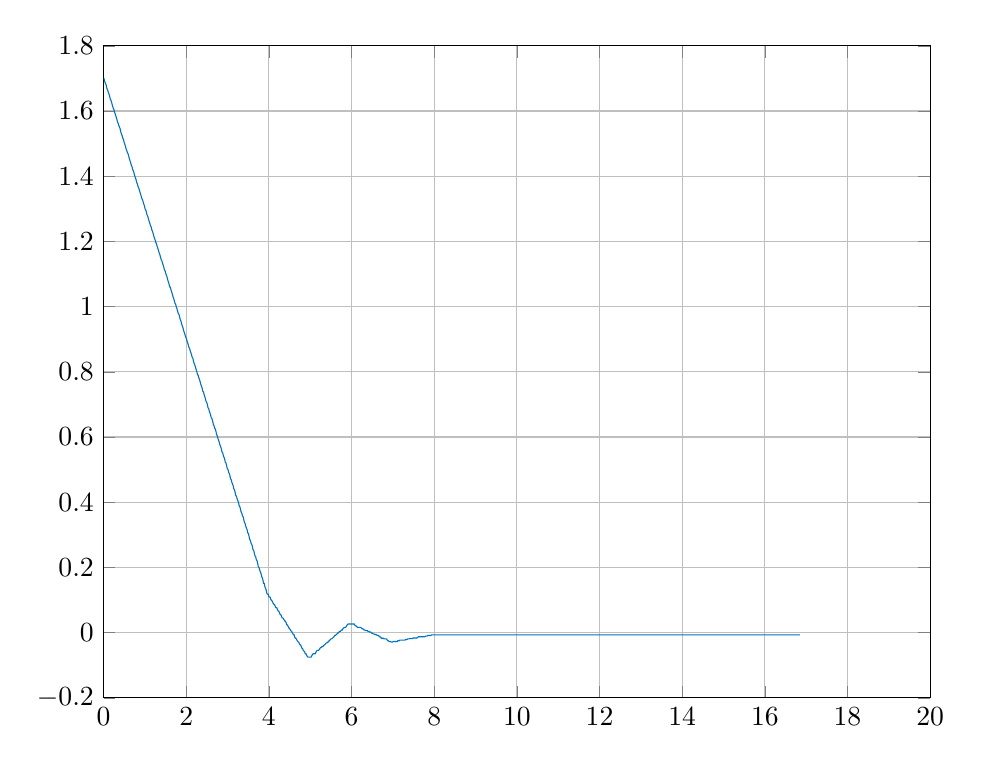
\begin{tikzpicture}

\begin{axis}[%
width=4.133in,
height=3.26in,
at={(0.693in,0.44in)},
scale only axis,
xmin=0,
xmax=20,
xmajorgrids,
ymin=-0.2,
ymax=1.8,
ymajorgrids,
axis background/.style={fill=white}
]
\addplot [color=mycolor1,solid,forget plot]
  table[row sep=crcr]{%
0	1.70285735290089\\
0.0157440119989999	1.69650943073385\\
0.0317904029989988	1.68875805435208\\
0.047723036998	1.6848853003827\\
0.063984608998999	1.67907024804334\\
0.079876580999	1.66938283441168\\
0.0969222959989998	1.66551024390915\\
0.112155140998	1.65818270513624\\
0.127915141999999	1.6533421242722\\
0.143694485997999	1.64752755929207\\
0.159706495999999	1.63784062821505\\
0.175837244997999	1.63396842308822\\
0.191750079999	1.62815411643423\\
0.209952186999999	1.61888606769363\\
0.225351247998999	1.61211128892162\\
0.240580861	1.60629724077087\\
0.255875798	1.60242521202517\\
0.271858255999999	1.59467522939827\\
0.287735118998999	1.58885878258392\\
0.303937432998	1.58204934358117\\
0.320593856999999	1.57523586459636\\
0.337111878999	1.56700022457241\\
0.352273449997999	1.56313121976515\\
0.367871633997999	1.55538197521956\\
0.383792919997999	1.55151051889807\\
0.399778857998999	1.54569738716581\\
0.415709069	1.53642675463401\\
0.431701561998	1.52965020599648\\
0.450088934999	1.52383717225652\\
0.465230186999999	1.5160858952691\\
0.480238291998999	1.5141530676449\\
0.495977407999	1.50446912632444\\
0.511778586998999	1.49907699501034\\
0.528150598998999	1.49229100110594\\
0.543860795999	1.48454024731062\\
0.559932518998999	1.47873656531568\\
0.575903753000001	1.47292430475764\\
0.591704024999	1.46905346813467\\
0.607768557998	1.46171818851001\\
0.623769505999999	1.45396803850555\\
0.639961316	1.44719000724728\\
0.655850686999999	1.44137804548545\\
0.671838214	1.43362826752217\\
0.687758874	1.4297604545746\\
0.703811777998999	1.42048853284756\\
0.719841370999999	1.41661828019\\
0.735811768998999	1.41031679958525\\
0.751877304	1.40208121640022\\
0.767864914998999	1.39627862347204\\
0.783853878999	1.3904675231347\\
0.799919025999	1.3811915695188\\
0.815791801999999	1.37732406418418\\
0.831872225	1.36957827474269\\
0.847851644997999	1.36473081324284\\
0.863725696998	1.35891998408175\\
0.879729358998999	1.35117165696314\\
0.896078924998999	1.34485312940149\\
0.911741382998999	1.33803001799782\\
0.930002520997999	1.33028212492097\\
0.945245803998999	1.32737123258858\\
0.960302719999	1.31962332197396\\
0.975735043997999	1.31382198353992\\
0.991725335997999	1.30749453327551\\
1.007728125999	1.29873313092044\\
1.025893224	1.29486663602312\\
1.040906092001	1.28663023820507\\
1.055994858999	1.28033428760386\\
1.071926370998	1.27646295730528\\
1.087724150999	1.26819822316578\\
1.10377318	1.26138235917247\\
1.119763156	1.25557275058097\\
1.135695288999	1.24782630194425\\
1.151884890998	1.24491306361134\\
1.167798546999	1.23523501985798\\
1.183787633998	1.23084781189134\\
1.199885359001	1.22402232668179\\
1.215866165	1.2162760433277\\
1.232075739999	1.21047622259384\\
1.248301617	1.20417406019494\\
1.264450319999	1.19593870682082\\
1.280442549999	1.19348822958045\\
1.295866743	1.18472495606981\\
1.312509360998	1.178925174867\\
1.327899553999	1.17311688703951\\
1.343812685998	1.1648777837991\\
1.359895796999	1.16052217858954\\
1.375768494998	1.15226034430333\\
1.391739391998	1.1454342987928\\
1.407806229999	1.14156513578168\\
1.423895379999	1.13382049370882\\
1.439740354999	1.12802171196122\\
1.455862361999	1.12122829334143\\
1.471833024	1.11296386755621\\
1.487723402999	1.11001225642607\\
1.503874188999	1.1022681146314\\
1.519867201999	1.09646949591101\\
1.535771678999	1.09066247656122\\
1.552086031	1.08242333422007\\
1.567790104999	1.07561249010977\\
1.58373003	1.06929424916183\\
1.599700420999	1.06104025429934\\
1.615805826999	1.05910936745059\\
1.631830441999	1.05136656152177\\
1.647697308	1.04507265588626\\
1.663874795999	1.03825207798216\\
1.679710784	1.03050938591575\\
1.695990473999	1.02562196901307\\
1.712010005998	1.01788211053564\\
1.727980546999	1.01013996889321\\
1.743812444999	1.00820952004993\\
1.759978391998	0.998955266710837\\
1.775858896999	0.993158277487796\\
1.791745733999	0.986327765860573\\
1.807911617998	0.978585729762072\\
1.823767645	0.976655458615085\\
1.839750108999	0.968914055652695\\
1.855734738998	0.960158728460848\\
1.871711081998	0.955797710883606\\
1.887680003	0.947030735298845\\
1.903727125999	0.941234206644054\\
1.919857000999	0.935428841763544\\
1.935874285999	0.927688440225307\\
1.951766531999	0.920870421485843\\
1.969185902	0.91457116874572\\
1.984232343999	0.907740558224004\\
1.999817252998	0.903873528113881\\
2.015722419	0.896132984527763\\
2.031769385999	0.890337861050211\\
2.047752260999	0.883510126499729\\
2.063874433	0.875275107298015\\
2.079781826999	0.872316848053943\\
2.095915288	0.864577022678879\\
2.111906060998	0.858781576982209\\
2.127914364999	0.852977680658902\\
2.143855075998	0.844713507701409\\
2.159761561	0.842284249775553\\
2.175801504999	0.833019723386752\\
2.191756566	0.825287417834138\\
2.207881139	0.821421102460963\\
2.223742774	0.813682035463674\\
2.23979051	0.807362495611214\\
2.255734256	0.801058848649527\\
2.271736375999	0.791793062974453\\
2.287874365999	0.789863689231774\\
2.303853461999	0.782125181492609\\
2.319738552999	0.776331003536485\\
2.335829378999	0.770002304063151\\
2.351872078998	0.76176342099465\\
2.367816330999	0.756372630342193\\
2.383817421999	0.750567062242333\\
2.399855701999	0.740900000362192\\
2.415943128999	0.738970609462516\\
2.43193325	0.730706808229083\\
2.447717246999	0.724412032257302\\
2.463743915998	0.717576280479064\\
2.479708935998	0.709341393597549\\
2.495740045999	0.705480480126474\\
2.511808929998	0.699675332300087\\
2.527847495998	0.689482143355576\\
2.543864431999	0.687553610790266\\
2.559831231	0.678280162590726\\
2.575817227998	0.673920723425189\\
2.591841069999	0.666187571783941\\
2.607804705999	0.65845119237603\\
2.623803586999	0.655994285535338\\
2.639842282999	0.648258904249714\\
2.655973328001	0.638991051357654\\
2.672110536998	0.634627329666198\\
2.687907486	0.6268918414139\\
2.703824034999	0.624963263738381\\
2.719955996997	0.616699075752305\\
2.735974692998	0.607035365483077\\
2.751948713001	0.603566263374225\\
2.767951797998	0.595331205215872\\
2.784004390998	0.58953978932461\\
2.799837019998	0.583739513027434\\
2.815815614999	0.575475127851398\\
2.831821716999	0.57161554800194\\
2.847803543998	0.56427034744401\\
2.863897149999	0.554607187001488\\
2.879805760999	0.552178329697082\\
2.895963828001	0.544444803354432\\
2.911907046999	0.538123615167373\\
2.927875734998	0.534252303897394\\
2.943891618	0.523046265382813\\
2.959949752998	0.521117889298677\\
2.975747796999	0.512883071678256\\
2.994024786998	0.502691186303577\\
3.009167035999	0.500762968193046\\
3.024129125	0.493029794662773\\
3.039751982999	0.488130053865556\\
3.055758731998	0.481822778190619\\
3.071845227998	0.471659642596423\\
3.087847312	0.469200978171759\\
3.103887659	0.461468404919254\\
3.119739446998	0.455678416372028\\
3.135695209999	0.450766003424904\\
3.151861003999	0.440599900936736\\
3.167671762001	0.438169446085264\\
3.183808695999	0.429905454527945\\
3.199700324001	0.420246175611374\\
3.215873379999	0.418318263156921\\
3.232042818	0.410064584938852\\
3.247735747999	0.405178624334876\\
3.265998639999	0.398874523425587\\
3.280976085998	0.388682798959474\\
3.296339593999	0.386755743272191\\
3.311962241998	0.379024578814147\\
3.327700757999	0.370255527784071\\
3.346093204999	0.365886647951282\\
3.361323958997	0.357652235605891\\
3.376701636999	0.355191470893919\\
3.391940134	0.347461657529002\\
3.407692600999	0.337803629596509\\
3.423937718999	0.334830027494068\\
3.439916349998	0.326592062640411\\
3.455893821998	0.320804768049964\\
3.471914331998	0.31589679901438\\
3.487928973999	0.306239828761512\\
3.503972087999	0.304313286547456\\
3.519795432001	0.295535933809726\\
3.535965377	0.285370343330743\\
3.551772534999	0.283444376419186\\
3.567912862999	0.27467516390367\\
3.584007997999	0.270818206146596\\
3.599847694999	0.265020125479368\\
3.615990944999	0.254314977476457\\
3.631801236	0.2523880009649\\
3.647988667999	0.243615838065979\\
3.664177569999	0.235388217177995\\
3.679684922	0.233454597341035\\
3.695905028999	0.223799964720179\\
3.711839462999	0.220823217016645\\
3.727980757	0.21309471405653\\
3.743956359998	0.202394804524943\\
3.759700784999	0.199962107210931\\
3.778195934999	0.192233964979423\\
3.793266900999	0.18643978010201\\
3.808764765998	0.181529733639637\\
3.824005274999	0.171875158618475\\
3.839728871	0.168901939564173\\
3.855779607999	0.161175729759427\\
3.871830118999	0.151014431303026\\
3.887925054998	0.151014911455691\\
3.904136244998	0.140309991345627\\
3.919804668998	0.136453810216266\\
3.935883129999	0.129608602942341\\
3.951798146999	0.119956691483946\\
3.969267685998	0.117522325204683\\
3.984276651998	0.117523178054442\\
3.999889670999	0.109797885369612\\
4.015766222	0.109798309739687\\
4.031773747999	0.107872524598938\\
4.050028864999	0.101022291764344\\
4.065226872999	0.0990941406756181\\
4.080286399999	0.0966294913780583\\
4.095730222999	0.0922509228520108\\
4.111807488998	0.0883935332502412\\
4.127906814001	0.0864675840689531\\
4.143752656	0.0845346570311047\\
4.159769248998	0.0782352266205741\\
4.175966850999	0.0763098953010106\\
4.191954752	0.076310938263618\\
4.208153529998	0.0705161221303472\\
4.223756538999	0.066662255390521\\
4.239802260997	0.0656063394415833\\
4.255983024	0.0611998240091409\\
4.271877678999	0.0554170863259424\\
4.287878789999	0.054904299363054\\
4.303736835998	0.0510387913870796\\
4.319836520999	0.0452565421296507\\
4.335874229999	0.0452575634711661\\
4.351839344999	0.0428147340851908\\
4.367834631	0.0389537880005228\\
4.383800339998	0.0351002216815051\\
4.399910986999	0.0351025310570541\\
4.41594618	0.0312372439308843\\
4.431689611999	0.0238525572623292\\
4.447842382	0.0238542785534874\\
4.463817097	0.0199890494691572\\
4.479911378997	0.0142074863029\\
4.495885710001	0.0136935492734049\\
4.511894208999	0.0098289546313719\\
4.52785867	0.00597661253246562\\
4.543788821998	0.0040495511042713\\
4.559803808	0.00160592760879674\\
4.575763288999	-0.00225003234435883\\
4.591826826999	-0.00610515797338529\\
4.607786983999	-0.00610353252762952\\
4.623874340997	-0.0135005137775537\\
4.639735261999	-0.0173559068478131\\
4.655733377998	-0.0173543140811767\\
4.671777930999	-0.0212191514982274\\
4.687894391998	-0.0255869691808615\\
4.703779736999	-0.0275133492187647\\
4.719756747999	-0.0294451520143202\\
4.73568744	-0.0333009481982669\\
4.751891691999	-0.0376672978338608\\
4.767985218	-0.0376661101861686\\
4.783759386999	-0.0434546461924505\\
4.799880669	-0.0478563201200268\\
4.815847882	-0.0489201603315212\\
4.831728426	-0.0547077346117897\\
4.847837493	-0.0566344487365111\\
4.863963596	-0.0585603746257826\\
4.879884944	-0.0648650979593182\\
4.895747435998	-0.0648637711647551\\
4.911832762998	-0.0687173621321984\\
4.927970750999	-0.0725721964740349\\
4.943919495	-0.0750166748254335\\
4.959920324998	-0.0750150300614409\\
4.975767406	-0.0750140865481297\\
4.991753791	-0.075013459663438\\
5.007844519998	-0.0750117820958491\\
5.023748593	-0.0750108276031849\\
5.039972913	-0.0706410496690382\\
5.055891355999	-0.0667800615791851\\
5.071908487999	-0.0648510323854858\\
5.087683378	-0.0648510323854858\\
5.105943022998	-0.0648493937482344\\
5.121129621	-0.0648486703222084\\
5.136304438999	-0.0604746400247078\\
5.15188418	-0.0566145134223976\\
5.167723607997	-0.0546853503178768\\
5.183803670999	-0.0546845554941886\\
5.199948204998	-0.0546840716142005\\
5.215883336998	-0.0527598061534684\\
5.231924673999	-0.0497575801281138\\
5.247864500999	-0.0458975557619379\\
5.263795357	-0.0458955268266821\\
5.279851007	-0.0434151157261891\\
5.295957586999	-0.0434143673711458\\
5.311918027999	-0.0414901681486091\\
5.327887534999	-0.0395581620632868\\
5.344199083999	-0.0376253707706895\\
5.359864420999	-0.0356972654252183\\
5.375885506	-0.0337688904469589\\
5.391859467998	-0.0313296444920432\\
5.407690223999	-0.0313276353155407\\
5.426018474998	-0.0293950313303926\\
5.441049194999	-0.0274631796778142\\
5.456691032999	-0.0255347167591236\\
5.471830202999	-0.0236072413979938\\
5.488132218998	-0.0211629011427839\\
5.50386317	-0.0192315339892966\\
5.519801427999	-0.0192293114741777\\
5.535706939998	-0.0172968212236324\\
5.551886961	-0.0153697877774055\\
5.567731529998	-0.013446062732815\\
5.583710011999	-0.0109641874239861\\
5.599788562999	-0.00795773201460981\\
5.615867225	-0.00795538538391738\\
5.631935512998	-0.00602281641801894\\
5.647754786998	-0.00410047690404203\\
5.664491264	-0.00217205201835302\\
5.679913639	-0.00024473407457748\\
5.695860906999	0.00168566452915453\\
5.711955434	0.00361934519389062\\
5.727986149999	0.00362090480548272\\
5.743921344999	0.00606183328351073\\
5.759717024999	0.00799009530652128\\
5.775791889999	0.00799099914671286\\
5.791654619998	0.0118482690933783\\
5.80775836	0.0137802084521257\\
5.823687874998	0.0157035456366492\\
5.839726306999	0.0162284172434137\\
5.855809988998	0.0162291492083031\\
5.871741779998	0.0181574446348001\\
5.887797635999	0.0225709085298156\\
5.903690736999	0.0245025929283864\\
5.919866378	0.0264258583898433\\
5.935830255998	0.0264269473047214\\
5.951850417999	0.0264276058818886\\
5.969312730999	0.0264299258649419\\
5.984323941	0.0264310250640174\\
5.999782619998	0.0264316939853362\\
6.015788441999	0.02643327098741\\
6.031835886999	0.0264351544215133\\
6.047887316	0.0264351544215133\\
6.063986475	0.0264374313458478\\
6.079767802999	0.0225880758083312\\
6.095829351999	0.0206625035180337\\
6.111694157999	0.0206639977947083\\
6.127656809999	0.018178234668824\\
6.144062059	0.0162538379324237\\
6.159885246	0.0162546323141231\\
6.175844982997	0.0162573537641189\\
6.191767027999	0.0162582563934428\\
6.207701266998	0.0162590611778608\\
6.223917191999	0.0157350778282064\\
6.239781586999	0.0138156958677789\\
6.255716998998	0.0118861124511591\\
6.271701753	0.0118886507739928\\
6.287734610998	0.00996447725258331\\
6.303685239999	0.00803609850883258\\
6.319762451999	0.0080387600730929\\
6.335853206998	0.00611488095756152\\
6.351892833999	0.00611488095756152\\
6.367831955999	0.00611757022843018\\
6.383784003997	0.00611964101130935\\
6.399683316999	0.00367559751554114\\
6.415852959999	0.00367831815499531\\
6.431803114997	0.00174898774173493\\
6.447865927	0.00175013770145926\\
6.463899278999	0.00175108927900625\\
6.479876875	-0.000171121410853958\\
6.496030646999	-0.00209889147601183\\
6.511723952999	-0.0020978345987217\\
6.527648567998	-0.00401963692874974\\
6.543810246	-0.0040184660163245\\
6.562214516998	-0.00593710714510975\\
6.575940565	-0.00593425198820774\\
6.592531036998	-0.00593297265756032\\
6.607893083999	-0.00786165290122764\\
6.623728055	-0.00785867448772293\\
6.639770745998	-0.00894650559391375\\
6.655928077999	-0.00894650559391375\\
6.672062421999	-0.0127960760057406\\
6.687775248998	-0.0133567790597917\\
6.703745034	-0.013355920899593\\
6.719842434999	-0.0171976367140954\\
6.735918643999	-0.0171956137117748\\
6.751726411998	-0.0171956137117748\\
6.768093562	-0.0171938550119113\\
6.783782704999	-0.0191212106990848\\
6.799715604999	-0.0191201260292659\\
6.815900615999	-0.0191192466793204\\
6.831869944	-0.0191161978379335\\
6.847749036998	-0.0191151025579352\\
6.863842257	-0.0229665514320005\\
6.879736219999	-0.0248824981400373\\
6.895858531999	-0.0254124061921379\\
6.911873529001	-0.0273352750146061\\
6.927836083	-0.0273323109860795\\
6.943856341999	-0.0273310961346376\\
6.959816676	-0.0292602109715532\\
6.977238718999	-0.0292581506977596\\
6.992281493999	-0.0292569251777857\\
7.007964947	-0.0273266662908533\\
7.023976653999	-0.0273257814170593\\
7.039794336999	-0.0273234300380012\\
7.055712229	-0.0273221725126565\\
7.071719670999	-0.0273212770006908\\
7.087692553999	-0.0273188936624795\\
7.105959587999	-0.0273176148004124\\
7.121230824998	-0.0248655819350543\\
7.136392067998	-0.0248632653981777\\
7.151788632999	-0.0248632653981777\\
7.167785630998	-0.0229343374268085\\
7.183926226999	-0.0229308288357277\\
7.199871787998	-0.0229308288357277\\
7.215909691999	-0.0229296062362729\\
7.231852443998	-0.0229260552403348\\
7.248059586999	-0.0229260552403348\\
7.263809225999	-0.0229248114214766\\
7.279873496999	-0.022922472449405\\
7.295745114997	-0.0229212180209022\\
7.311889229	-0.0209914843489329\\
7.327707649	-0.0209902924473597\\
7.343770798	-0.0209879410936684\\
7.359783098999	-0.0190693130497508\\
7.375692055999	-0.019068110585156\\
7.391690982999	-0.0190658267935326\\
7.409986698999	-0.0184949147912421\\
7.425247597	-0.0184937017636626\\
7.440536222	-0.0184910517107064\\
7.455911244998	-0.0184910517107064\\
7.471819201999	-0.0184894879569268\\
7.487835598999	-0.0165585084615114\\
7.503731652	-0.0165585084615114\\
7.519808541997	-0.0165569236406551\\
7.535998180999	-0.0165530696040213\\
7.551851592998	-0.0165530696040213\\
7.56788969	-0.0165514637162822\\
7.583867999998	-0.0165491839665279\\
7.599738684999	-0.0146311219613606\\
7.615828602998	-0.0127016824224855\\
7.631830159999	-0.0126994745074889\\
7.647774369998	-0.0126979369481721\\
7.663928854	-0.0126963889140077\\
7.679980058998	-0.0126952166787058\\
7.695813427	-0.0126926014814683\\
7.711861461	-0.0126910324977505\\
7.727809775999	-0.0126898497583814\\
7.743934729	-0.0126872031072427\\
7.759788016998	-0.0126872031072427\\
7.775961493	-0.0126856131741631\\
7.791930059	-0.0107552290682638\\
7.807851578998	-0.0107552290682638\\
7.823705771999	-0.0107536181860155\\
7.839894232999	-0.00883435440556291\\
7.855688417999	-0.00883435440556291\\
7.872108229999	-0.00883282302796218\\
7.887771111999	-0.00882906211847834\\
7.904009326997	-0.00882906211847834\\
7.919739838998	-0.00882750990879066\\
7.935757836999	-0.00689800893700476\\
7.951773984001	-0.00689644631134434\\
7.969244658001	-0.00689487326975868\\
7.984493156	-0.00689487326975868\\
7.999891401001	-0.00689487326975868\\
8.015860794	-0.00689487326975868\\
8.034486337999	-0.00689487326975868\\
8.049693639999	-0.00689487326975868\\
8.064870004999	-0.00689487326975868\\
8.080131097999	-0.00689487326975868\\
8.095896999	-0.00689487326975868\\
8.111725136999	-0.00689487326975868\\
8.127730461	-0.00689487326975868\\
8.146075710998	-0.00689487326975868\\
8.161129274999	-0.00689487326975868\\
8.176185378	-0.00689487326975868\\
8.191889491998	-0.00689487326975868\\
8.207864417999	-0.00689487326975868\\
8.223832333999	-0.00689487326975868\\
8.239944941999	-0.00689487326975868\\
8.255831359998	-0.00689487326975868\\
8.271803393999	-0.00689487326975868\\
8.287801122999	-0.00689487326975868\\
8.303864833999	-0.00689487326975868\\
8.319931889999	-0.00689487326975868\\
8.335831862999	-0.00689487326975868\\
8.352112781999	-0.00689487326975868\\
8.367842897998	-0.00689487326975868\\
8.383850731	-0.00689487326975868\\
8.399905497999	-0.00689487326975868\\
8.415712517	-0.00689487326975868\\
8.434013729	-0.00689487326975868\\
8.449407303999	-0.00689487326975868\\
8.464561392	-0.00689487326975868\\
8.479773770998	-0.00689487326975868\\
8.495937296999	-0.00689487326975868\\
8.511857499998	-0.00689487326975868\\
8.527876669	-0.00689487326975868\\
8.543763750999	-0.00689487326975868\\
8.559881512001	-0.00689487326975868\\
8.575977915998	-0.00689487326975868\\
8.592008475999	-0.00689487326975868\\
8.607691295	-0.00689487326975868\\
8.62367869	-0.00689487326975868\\
8.639769267999	-0.00689487326975868\\
8.658068563999	-0.00689487326975868\\
8.673209795999	-0.00689487326975868\\
8.688556534999	-0.00689487326975868\\
8.703823871999	-0.00689487326975868\\
8.719898443998	-0.00689487326975868\\
8.735824501998	-0.00689487326975868\\
8.751858395	-0.00689487326975868\\
8.767870095998	-0.00689487326975868\\
8.783829515998	-0.00689487326975868\\
8.799855868999	-0.00689487326975868\\
8.815806	-0.00689487326975868\\
8.831800475999	-0.00689487326975868\\
8.847834199998	-0.00689487326975868\\
8.863821559999	-0.00689487326975868\\
8.87985753	-0.00689487326975868\\
8.895970339	-0.00689487326975868\\
8.911950045999	-0.00689487326975868\\
8.927989735	-0.00689487326975868\\
8.94396394	-0.00689487326975868\\
8.959864371999	-0.00689487326975868\\
8.975965433	-0.00689487326975868\\
8.991975451	-0.00689487326975868\\
9.008038114999	-0.00689487326975868\\
9.023961167999	-0.00689487326975868\\
9.039850971	-0.00689487326975868\\
9.055872522998	-0.00689487326975868\\
9.071960899999	-0.00689487326975868\\
9.087998312999	-0.00689487326975868\\
9.103847584999	-0.00689487326975868\\
9.119834357999	-0.00689487326975868\\
9.135937755998	-0.00689487326975868\\
9.152083795999	-0.00689487326975868\\
9.167963375999	-0.00689487326975868\\
9.183992364999	-0.00689487326975868\\
9.199994046999	-0.00689487326975868\\
9.215889524	-0.00689487326975868\\
9.231794617	-0.00689487326975868\\
9.247849385	-0.00689487326975868\\
9.263833702999	-0.00689487326975868\\
9.279780369998	-0.00689487326975868\\
9.295947591999	-0.00689487326975868\\
9.311906757999	-0.00689487326975868\\
9.327866839	-0.00689487326975868\\
9.343852593999	-0.00689487326975868\\
9.359769629999	-0.00689487326975868\\
9.378122437999	-0.00689487326975868\\
9.393331143999	-0.00689487326975868\\
9.408447348999	-0.00689487326975868\\
9.423885301	-0.00689487326975868\\
9.439686055999	-0.00689487326975868\\
9.455854339998	-0.00689487326975868\\
9.471856151998	-0.00689487326975868\\
9.488563480999	-0.00689487326975868\\
9.503758071998	-0.00689487326975868\\
9.51975384	-0.00689487326975868\\
9.535688684999	-0.00689487326975868\\
9.551683746999	-0.00689487326975868\\
9.567794732999	-0.00689487326975868\\
9.583757032999	-0.00689487326975868\\
9.599802284999	-0.00689487326975868\\
9.616035258998	-0.00689487326975868\\
9.631880701999	-0.00689487326975868\\
9.649169075	-0.00689487326975868\\
9.664743880998	-0.00689487326975868\\
9.679858027999	-0.00689487326975868\\
9.695876861999	-0.00689487326975868\\
9.711820004999	-0.00689487326975868\\
9.727902131	-0.00689487326975868\\
9.743725618999	-0.00689487326975868\\
9.759725927999	-0.00689487326975868\\
9.775902572	-0.00689487326975868\\
9.791694743	-0.00689487326975868\\
9.807865850999	-0.00689487326975868\\
9.82385027	-0.00689487326975868\\
9.840151108999	-0.00689487326975868\\
9.855932195999	-0.00689487326975868\\
9.872397148998	-0.00689487326975868\\
9.887776386999	-0.00689487326975868\\
9.903872680997	-0.00689487326975868\\
9.919913677999	-0.00689487326975868\\
9.93583711	-0.00689487326975868\\
9.951928673997	-0.00689487326975868\\
9.969462458	-0.00689487326975868\\
9.984669364999	-0.00689487326975868\\
9.999850510999	-0.00689487326975868\\
10.016067917999	-0.00689487326975868\\
10.031682302999	-0.00689487326975868\\
10.047713083999	-0.00689487326975868\\
10.063753760999	-0.00689487326975868\\
10.082168945999	-0.00689487326975868\\
10.097433676998	-0.00689487326975868\\
10.112873338998	-0.00689487326975868\\
10.127949504999	-0.00689487326975868\\
10.144023403999	-0.00689487326975868\\
10.159839951999	-0.00689487326975868\\
10.175942265998	-0.00689487326975868\\
10.191857621997	-0.00689487326975868\\
10.20777434	-0.00689487326975868\\
10.223778600999	-0.00689487326975868\\
10.239847990999	-0.00689487326975868\\
10.255875368	-0.00689487326975868\\
10.271904661998	-0.00689487326975868\\
10.287881748998	-0.00689487326975868\\
10.303914425998	-0.00689487326975868\\
10.319733404998	-0.00689487326975868\\
10.336015230999	-0.00689487326975868\\
10.351738396999	-0.00689487326975868\\
10.367857145999	-0.00689487326975868\\
10.383715284999	-0.00689487326975868\\
10.399746984998	-0.00689487326975868\\
10.415680990999	-0.00689487326975868\\
10.431671256	-0.00689487326975868\\
10.447856169	-0.00689487326975868\\
10.463931509	-0.00689487326975868\\
10.479832600999	-0.00689487326975868\\
10.495879817998	-0.00689487326975868\\
10.511927493999	-0.00689487326975868\\
10.527733031999	-0.00689487326975868\\
10.543790600999	-0.00689487326975868\\
10.559919302	-0.00689487326975868\\
10.5759305	-0.00689487326975868\\
10.591983237999	-0.00689487326975868\\
10.607707379999	-0.00689487326975868\\
10.623887277	-0.00689487326975868\\
10.639937399	-0.00689487326975868\\
10.655951274	-0.00689487326975868\\
10.671742628999	-0.00689487326975868\\
10.689996191999	-0.00689487326975868\\
10.70538253	-0.00689487326975868\\
10.719690619998	-0.00689487326975868\\
10.735704902	-0.00689487326975868\\
10.751883691	-0.00689487326975868\\
10.767951452999	-0.00689487326975868\\
10.783952564001	-0.00689487326975868\\
10.799689850999	-0.00689487326975868\\
10.815679774	-0.00689487326975868\\
10.831921965	-0.00689487326975868\\
10.847685967998	-0.00689487326975868\\
10.863937288	-0.00689487326975868\\
10.879931025999	-0.00689487326975868\\
10.895851559	-0.00689487326975868\\
10.911939617	-0.00689487326975868\\
10.928118865999	-0.00689487326975868\\
10.943861892999	-0.00689487326975868\\
10.959729966999	-0.00689487326975868\\
10.976299722999	-0.00689487326975868\\
10.991711486999	-0.00689487326975868\\
11.007893629999	-0.00689487326975868\\
11.023745524999	-0.00689487326975868\\
11.039821934999	-0.00689487326975868\\
11.055834612999	-0.00689487326975868\\
11.07185702	-0.00689487326975868\\
11.088183551998	-0.00689487326975868\\
11.103975784999	-0.00689487326975868\\
11.119803784999	-0.00689487326975868\\
11.135932549999	-0.00689487326975868\\
11.151696129999	-0.00689487326975868\\
11.167689359001	-0.00689487326975868\\
11.183840634998	-0.00689487326975868\\
11.199700031999	-0.00689487326975868\\
11.217974452999	-0.00689487326975868\\
11.233021660999	-0.00689487326975868\\
11.248146020999	-0.00689487326975868\\
11.263858203998	-0.00689487326975868\\
11.279896968	-0.00689487326975868\\
11.295786261999	-0.00689487326975868\\
11.311814746	-0.00689487326975868\\
11.327892843998	-0.00689487326975868\\
11.343741857	-0.00689487326975868\\
11.36194851	-0.00689487326975868\\
11.377220669	-0.00689487326975868\\
11.392557418998	-0.00689487326975868\\
11.407861384998	-0.00689487326975868\\
11.423805137998	-0.00689487326975868\\
11.439871917999	-0.00689487326975868\\
11.455831025999	-0.00689487326975868\\
11.471800750999	-0.00689487326975868\\
11.487794873998	-0.00689487326975868\\
11.503817603	-0.00689487326975868\\
11.519751711	-0.00689487326975868\\
11.535731101999	-0.00689487326975868\\
11.551737834999	-0.00689487326975868\\
11.567860666999	-0.00689487326975868\\
11.583865694999	-0.00689487326975868\\
11.599911237999	-0.00689487326975868\\
11.615881372999	-0.00689487326975868\\
11.631847639999	-0.00689487326975868\\
11.647740637998	-0.00689487326975868\\
11.664127391998	-0.00689487326975868\\
11.679745422998	-0.00689487326975868\\
11.695734422998	-0.00689487326975868\\
11.711901465999	-0.00689487326975868\\
11.727832562	-0.00689487326975868\\
11.743896906	-0.00689487326975868\\
11.759918630998	-0.00689487326975868\\
11.775866122999	-0.00689487326975868\\
11.791844917999	-0.00689487326975868\\
11.807741026998	-0.00689487326975868\\
11.823930274999	-0.00689487326975868\\
11.839728063999	-0.00689487326975868\\
11.855891316999	-0.00689487326975868\\
11.871869225999	-0.00689487326975868\\
11.887842913999	-0.00689487326975868\\
11.903886365999	-0.00689487326975868\\
11.919971385	-0.00689487326975868\\
11.935770383998	-0.00689487326975868\\
11.951697043998	-0.00689487326975868\\
11.969028198999	-0.00689487326975868\\
11.984303704	-0.00689487326975868\\
11.999850389999	-0.00689487326975868\\
12.015863534	-0.00689487326975868\\
12.031785208999	-0.00689487326975868\\
12.047680946998	-0.00689487326975868\\
12.066133161998	-0.00689487326975868\\
12.081355899999	-0.00689487326975868\\
12.096501429998	-0.00689487326975868\\
12.111701831998	-0.00689487326975868\\
12.127671705999	-0.00689487326975868\\
12.145995091999	-0.00689487326975868\\
12.160637378999	-0.00689487326975868\\
12.175787900999	-0.00689487326975868\\
12.191988152	-0.00689487326975868\\
12.208532983999	-0.00689487326975868\\
12.223890896999	-0.00689487326975868\\
12.239949820999	-0.00689487326975868\\
12.255854152998	-0.00689487326975868\\
12.271915221	-0.00689487326975868\\
12.287712510999	-0.00689487326975868\\
12.303839073999	-0.00689487326975868\\
12.319682246999	-0.00689487326975868\\
12.335952984998	-0.00689487326975868\\
12.351849372999	-0.00689487326975868\\
12.367837177	-0.00689487326975868\\
12.383972798999	-0.00689487326975868\\
12.400012392999	-0.00689487326975868\\
12.418440679	-0.00689487326975868\\
12.433596468999	-0.00689487326975868\\
12.448673385	-0.00689487326975868\\
12.463987995	-0.00689487326975868\\
12.480013010999	-0.00689487326975868\\
12.495770630998	-0.00689487326975868\\
12.51186779	-0.00689487326975868\\
12.528012049999	-0.00689487326975868\\
12.543727267	-0.00689487326975868\\
12.559865478	-0.00689487326975868\\
12.575911650999	-0.00689487326975868\\
12.591816892999	-0.00689487326975868\\
12.607828970998	-0.00689487326975868\\
12.624861232999	-0.00689487326975868\\
12.639911784998	-0.00689487326975868\\
12.655678377998	-0.00689487326975868\\
12.671691270999	-0.00689487326975868\\
12.687805221998	-0.00689487326975868\\
12.703758333999	-0.00689487326975868\\
12.719944017999	-0.00689487326975868\\
12.735782854	-0.00689487326975868\\
12.751747464	-0.00689487326975868\\
12.767757910999	-0.00689487326975868\\
12.783720473999	-0.00689487326975868\\
12.799691989999	-0.00689487326975868\\
12.815735457998	-0.00689487326975868\\
12.831869028999	-0.00689487326975868\\
12.847880298	-0.00689487326975868\\
12.863878718	-0.00689487326975868\\
12.880160594999	-0.00689487326975868\\
12.895689042999	-0.00689487326975868\\
12.911862537998	-0.00689487326975868\\
12.927921642999	-0.00689487326975868\\
12.943806774	-0.00689487326975868\\
12.960424625999	-0.00689487326975868\\
12.975783403999	-0.00689487326975868\\
12.991979361	-0.00689487326975868\\
13.007741114	-0.00689487326975868\\
13.023848452999	-0.00689487326975868\\
13.039946362999	-0.00689487326975868\\
13.055851556999	-0.00689487326975868\\
13.071815931999	-0.00689487326975868\\
13.087910456998	-0.00689487326975868\\
13.103690725999	-0.00689487326975868\\
13.119683629999	-0.00689487326975868\\
13.137922500999	-0.00689487326975868\\
13.153127126998	-0.00689487326975868\\
13.168186093999	-0.00689487326975868\\
13.183824262998	-0.00689487326975868\\
13.199886836999	-0.00689487326975868\\
13.215675777	-0.00689487326975868\\
13.231800368999	-0.00689487326975868\\
13.247795038999	-0.00689487326975868\\
13.264110188999	-0.00689487326975868\\
13.279888559	-0.00689487326975868\\
13.295814115999	-0.00689487326975868\\
13.311693557998	-0.00689487326975868\\
13.327936698	-0.00689487326975868\\
13.343932927	-0.00689487326975868\\
13.359910389	-0.00689487326975868\\
13.375916663	-0.00689487326975868\\
13.391915162	-0.00689487326975868\\
13.407734337999	-0.00689487326975868\\
13.423927767999	-0.00689487326975868\\
13.439781073	-0.00689487326975868\\
13.455788980999	-0.00689487326975868\\
13.471859537998	-0.00689487326975868\\
13.487721312999	-0.00689487326975868\\
13.503873605999	-0.00689487326975868\\
13.519824607999	-0.00689487326975868\\
13.535716282999	-0.00689487326975868\\
13.551768087999	-0.00689487326975868\\
13.567852916999	-0.00689487326975868\\
13.583737838998	-0.00689487326975868\\
13.599886993	-0.00689487326975868\\
13.615774641998	-0.00689487326975868\\
13.631868470998	-0.00689487326975868\\
13.647757930999	-0.00689487326975868\\
13.663845691	-0.00689487326975868\\
13.679729730999	-0.00689487326975868\\
13.695803116998	-0.00689487326975868\\
13.712631680999	-0.00689487326975868\\
13.727922558	-0.00689487326975868\\
13.744237890998	-0.00689487326975868\\
13.759832027	-0.00689487326975868\\
13.775790274999	-0.00689487326975868\\
13.792044622999	-0.00689487326975868\\
13.807895728998	-0.00689487326975868\\
13.823775414999	-0.00689487326975868\\
13.842056048999	-0.00689487326975868\\
13.857211182998	-0.00689487326975868\\
13.872399034999	-0.00689487326975868\\
13.887732146999	-0.00689487326975868\\
13.903710759	-0.00689487326975868\\
13.919779392	-0.00689487326975868\\
13.935923931999	-0.00689487326975868\\
13.951898822	-0.00689487326975868\\
13.969342035999	-0.00689487326975868\\
13.984470385999	-0.00689487326975868\\
13.999721986999	-0.00689487326975868\\
14.015876871999	-0.00689487326975868\\
14.031777448999	-0.00689487326975868\\
14.047798769001	-0.00689487326975868\\
14.063769788999	-0.00689487326975868\\
14.079808093999	-0.00689487326975868\\
14.095678835998	-0.00689487326975868\\
14.111897218998	-0.00689487326975868\\
14.128133427999	-0.00689487326975868\\
14.144516714998	-0.00689487326975868\\
14.160049152999	-0.00689487326975868\\
14.175911404998	-0.00689487326975868\\
14.191870836	-0.00689487326975868\\
14.207701133998	-0.00689487326975868\\
14.223693989	-0.00689487326975868\\
14.239882217998	-0.00689487326975868\\
14.255733864999	-0.00689487326975868\\
14.271898906999	-0.00689487326975868\\
14.287717454	-0.00689487326975868\\
14.303683077999	-0.00689487326975868\\
14.321935461	-0.00689487326975868\\
14.337294693998	-0.00689487326975868\\
14.352464480999	-0.00689487326975868\\
14.367848416	-0.00689487326975868\\
14.383902388	-0.00689487326975868\\
14.399832027999	-0.00689487326975868\\
14.415820937999	-0.00689487326975868\\
14.431739605999	-0.00689487326975868\\
14.447856400999	-0.00689487326975868\\
14.463883937999	-0.00689487326975868\\
14.479735664999	-0.00689487326975868\\
14.49608917	-0.00689487326975868\\
14.511956542999	-0.00689487326975868\\
14.527900933	-0.00689487326975868\\
14.543733062999	-0.00689487326975868\\
14.562121685998	-0.00689487326975868\\
14.577401333999	-0.00689487326975868\\
14.592625791999	-0.00689487326975868\\
14.607976794	-0.00689487326975868\\
14.623736511999	-0.00689487326975868\\
14.639688777	-0.00689487326975868\\
14.655958072	-0.00689487326975868\\
14.671801726999	-0.00689487326975868\\
14.687870781	-0.00689487326975868\\
14.703807581998	-0.00689487326975868\\
14.719913893999	-0.00689487326975868\\
14.735864476999	-0.00689487326975868\\
14.751883903999	-0.00689487326975868\\
14.767817878	-0.00689487326975868\\
14.783929946001	-0.00689487326975868\\
14.799811580999	-0.00689487326975868\\
14.815821753999	-0.00689487326975868\\
14.831694913	-0.00689487326975868\\
14.847692405998	-0.00689487326975868\\
14.863738395	-0.00689487326975868\\
14.879935740999	-0.00689487326975868\\
14.895865977998	-0.00689487326975868\\
14.911881269998	-0.00689487326975868\\
14.927901737999	-0.00689487326975868\\
14.943731604999	-0.00689487326975868\\
14.959861101999	-0.00689487326975868\\
14.975888172	-0.00689487326975868\\
14.992376180999	-0.00689487326975868\\
15.007905333	-0.00689487326975868\\
15.024405805	-0.00689487326975868\\
15.039787382999	-0.00689487326975868\\
15.055791885997	-0.00689487326975868\\
15.071847990999	-0.00689487326975868\\
15.087734774999	-0.00689487326975868\\
15.103856102998	-0.00689487326975868\\
15.119847077999	-0.00689487326975868\\
15.136156173	-0.00689487326975868\\
15.151833694999	-0.00689487326975868\\
15.167806411998	-0.00689487326975868\\
15.183935973999	-0.00689487326975868\\
15.199858121	-0.00689487326975868\\
15.215841121	-0.00689487326975868\\
15.231910250999	-0.00689487326975868\\
15.247896238	-0.00689487326975868\\
15.263852080999	-0.00689487326975868\\
15.279843970998	-0.00689487326975868\\
15.295828844999	-0.00689487326975868\\
15.311799476999	-0.00689487326975868\\
15.327847304	-0.00689487326975868\\
15.343820857	-0.00689487326975868\\
15.359935775999	-0.00689487326975868\\
15.375914555999	-0.00689487326975868\\
15.391861423999	-0.00689487326975868\\
15.407749382	-0.00689487326975868\\
15.423983988	-0.00689487326975868\\
15.439864055	-0.00689487326975868\\
15.455838329999	-0.00689487326975868\\
15.471875388	-0.00689487326975868\\
15.487774885999	-0.00689487326975868\\
15.503962505001	-0.00689487326975868\\
15.519877772998	-0.00689487326975868\\
15.535855301	-0.00689487326975868\\
15.551861337999	-0.00689487326975868\\
15.567905732	-0.00689487326975868\\
15.583867864	-0.00689487326975868\\
15.599844850999	-0.00689487326975868\\
15.615968996	-0.00689487326975868\\
15.631910205999	-0.00689487326975868\\
15.647759424999	-0.00689487326975868\\
15.663711198999	-0.00689487326975868\\
15.679875220998	-0.00689487326975868\\
15.695761545	-0.00689487326975868\\
15.711704864999	-0.00689487326975868\\
15.727708413999	-0.00689487326975868\\
15.743841247999	-0.00689487326975868\\
15.759760488	-0.00689487326975868\\
15.775865729999	-0.00689487326975868\\
15.791700076	-0.00689487326975868\\
15.807817968999	-0.00689487326975868\\
15.825016185998	-0.00689487326975868\\
15.840248537	-0.00689487326975868\\
15.855870848999	-0.00689487326975868\\
15.871831740999	-0.00689487326975868\\
15.887675523	-0.00689487326975868\\
15.906153020999	-0.00689487326975868\\
15.921390501998	-0.00689487326975868\\
15.936582784	-0.00689487326975868\\
15.951890282999	-0.00689487326975868\\
15.969464925998	-0.00689487326975868\\
15.984697470001	-0.00689487326975868\\
15.999900396999	-0.00689487326975868\\
16.015863240999	-0.00689487326975868\\
16.031855681999	-0.00689487326975868\\
16.047711413999	-0.00689487326975868\\
16.063700975999	-0.00689487326975868\\
16.079713595998	-0.00689487326975868\\
16.095685989999	-0.00689487326975868\\
16.111870552	-0.00689487326975868\\
16.12790862	-0.00689487326975868\\
16.143795969999	-0.00689487326975868\\
16.159932718998	-0.00689487326975868\\
16.175801815998	-0.00689487326975868\\
16.191885047998	-0.00689487326975868\\
16.207842072	-0.00689487326975868\\
16.223679378999	-0.00689487326975868\\
16.242041708999	-0.00689487326975868\\
16.257124671999	-0.00689487326975868\\
16.272438057998	-0.00689487326975868\\
16.287951899	-0.00689487326975868\\
16.303908293998	-0.00689487326975868\\
16.319833962999	-0.00689487326975868\\
16.335870103998	-0.00689487326975868\\
16.351850693998	-0.00689487326975868\\
16.367804933998	-0.00689487326975868\\
16.383796768999	-0.00689487326975868\\
16.399924127	-0.00689487326975868\\
16.415785328001	-0.00689487326975868\\
16.431812504999	-0.00689487326975868\\
16.447678223999	-0.00689487326975868\\
16.463710534	-0.00689487326975868\\
16.482026591999	-0.00689487326975868\\
16.497179496999	-0.00689487326975868\\
16.512346711999	-0.00689487326975868\\
16.527927238998	-0.00689487326975868\\
16.543967243	-0.00689487326975868\\
16.55973185	-0.00689487326975868\\
16.575905024	-0.00689487326975868\\
16.591779776001	-0.00689487326975868\\
16.607796336999	-0.00689487326975868\\
16.623701105999	-0.00689487326975868\\
16.639861769998	-0.00689487326975868\\
16.655727007	-0.00689487326975868\\
16.671779145	-0.00689487326975868\\
16.687883048999	-0.00689487326975868\\
16.703920327999	-0.00689487326975868\\
16.719726902999	-0.00689487326975868\\
16.735767473999	-0.00689487326975868\\
16.751883116998	-0.00689487326975868\\
16.767830935998	-0.00689487326975868\\
16.783878923	-0.00689487326975868\\
16.799832913	-0.00689487326975868\\
16.815823364999	-0.00689487326975868\\
16.831902236999	-0.00689487326975868\\
16.847836177999	-0.00689487326975868\\
};
\end{axis}
\end{tikzpicture}%}
      \caption{The error in displacement of the robot over time for
        $(K_{\Psi}^R, K_{\omega}^T) \equiv (0.5 K_{\Psi, max}^R, 0.75 K_{\omega, max}^T)$}
      \label{fig:19_12_distance}
    \end{figure}
  \end{minipage}
  \hfill
  \begin{minipage}{0.45\linewidth}
    \begin{figure}[H]
      \scalebox{0.6}{% This file was created by matlab2tikz.
%
%The latest updates can be retrieved from
%  http://www.mathworks.com/matlabcentral/fileexchange/22022-matlab2tikz-matlab2tikz
%where you can also make suggestions and rate matlab2tikz.
%
\definecolor{mycolor1}{rgb}{0.00000,0.44700,0.74100}%
%
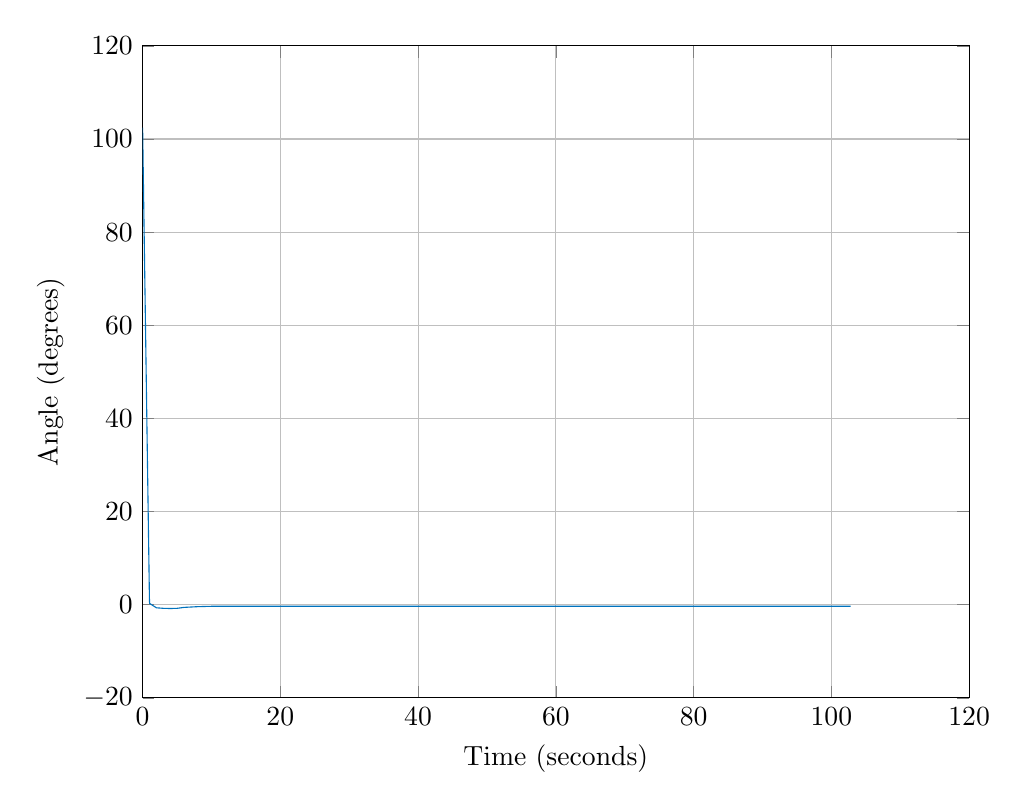
\begin{tikzpicture}

\begin{axis}[%
width=4.133in,
height=3.26in,
at={(0.693in,0.44in)},
scale only axis,
xmin=0,
xmax=120,
xmajorgrids,
xlabel={Time (seconds)},
ymin=-20,
ymax=120,
ymajorgrids,
ylabel={Angle (degrees)},
axis background/.style={fill=white}
]
\addplot [color=mycolor1,solid,forget plot]
  table[row sep=crcr]{%
0	102.4204\\
0.0180339650009992	101.6864\\
0.0317542980009997	100.1644\\
0.049851544001	98.5344\\
0.0648359720000001	96.9704\\
0.0797620589999994	95.3944\\
0.0958450539999995	93.7844\\
0.111878317	92.1404\\
0.127792176999999	90.5104\\
0.143880708001	88.8644\\
0.159875211999999	87.2244\\
0.175891278	85.5944\\
0.191880843001	83.9404\\
0.207873390001	82.2624\\
0.223881833001	80.6544\\
0.239873373	79.0204\\
0.255875306000999	77.3964\\
0.271861183999999	75.7904\\
0.287878221	74.1584\\
0.303847886	72.5184\\
0.319869886	70.8264\\
0.335865359000999	69.2004\\
0.351809091000999	67.5884\\
0.369865824000999	65.9004\\
0.385202440001	64.2784\\
0.400454655001	62.6464\\
0.415878348999999	61.0324\\
0.431894534000999	59.4184\\
0.447867557000999	57.7864\\
0.463870869001	56.1464\\
0.479836335	54.5044\\
0.495835156	52.8664\\
0.511908702001999	51.2404\\
0.527864456001	49.5804\\
0.54387571	47.9584\\
0.559874977000999	46.3164\\
0.575999929000999	44.6184\\
0.591991242	42.9924\\
0.607830894	41.3784\\
0.623809344	39.7144\\
0.639993135000999	38.1004\\
0.656064239999999	36.4524\\
0.672025376000999	34.8424\\
0.688021834	33.2224\\
0.704047861	31.5884\\
0.720080399001	29.9404\\
0.735993350000999	28.3004\\
0.751935345001	26.6684\\
0.768155561	25.0504\\
0.783859850000999	23.3984\\
0.799870508000999	21.7644\\
0.815886638001	20.1564\\
0.831872951000999	18.5104\\
0.847860096	16.8484\\
0.863717640001	15.2384\\
0.880031136000999	13.5804\\
0.895959565000999	11.9504\\
0.911988572001	10.3304\\
0.928015669000999	8.69239999999999\\
0.944012611	7.0104\\
0.960040944000999	5.38039999999999\\
0.976021223001	3.7544\\
0.992004720001	2.0864\\
1.007800683001	0.710399999999993\\
1.026041016	0.2684\\
1.041350275001	0.252399999999994\\
1.056335854	0.238399999999999\\
1.071742401	0.222399999999993\\
1.087796375	0.208399999999997\\
1.103864198001	0.194400000000002\\
1.119875239001	0.178399999999996\\
1.135813953	0.162400000000005\\
1.151910246001	0.1464\\
1.167870715001	0.13239999999999\\
1.18387299	0.118399999999994\\
1.199905387	0.102400000000003\\
1.215880956	0.0863999999999976\\
1.231886673001	0.0703999999999922\\
1.247918634	0.0563999999999965\\
1.263899495001	0.0404000000000053\\
1.279944316	0.0263999999999953\\
1.295907546001	0.0103999999999758\\
1.311908116001	-0.00560000000000116\\
1.32790104	-0.0196000000000112\\
1.344167688001	-0.0375999999999976\\
1.359888865001	-0.0496000000000123\\
1.375759407001	-0.0656000000000176\\
1.39174587	-0.0836000000000041\\
1.408022415	-0.0976000000000141\\
1.423765840001	-0.111599999999996\\
1.439863397001	-0.125600000000006\\
1.455863173	-0.141600000000011\\
1.472124863001	-0.159599999999998\\
1.488016266	-0.173600000000008\\
1.504008632	-0.187600000000018\\
1.520013252001	-0.203600000000009\\
1.536000758001	-0.217600000000019\\
1.552061089	-0.233599999999996\\
1.568054152	-0.247600000000006\\
1.583989257	-0.26560000000002\\
1.59974975	-0.279600000000002\\
1.617839823001	-0.295600000000007\\
1.633130521	-0.309600000000003\\
1.648667386	-0.325600000000009\\
1.664245496001	-0.339600000000019\\
1.680031153	-0.3536\\
1.696255079001	-0.36960000000002\\
1.712023108	-0.385599999999997\\
1.727999203	-0.401600000000002\\
1.7440227	-0.415600000000012\\
1.760117985	-0.429600000000008\\
1.77601454	-0.445600000000013\\
1.792033471	-0.461600000000004\\
1.807942565001	-0.47760000000001\\
1.826371135001	-0.49160000000002\\
1.841891602001	-0.505600000000001\\
1.857197905001	-0.521600000000007\\
1.872929905	-0.537599999999998\\
1.888347001	-0.553600000000003\\
1.904030382	-0.567600000000013\\
1.920075203	-0.583600000000004\\
1.936037923001	-0.597600000000014\\
1.952049508	-0.613599999999991\\
1.968120773	-0.629600000000011\\
1.984032437001	-0.645600000000016\\
2.000018129	-0.657600000000002\\
2.018059051	-0.669600000000017\\
2.031786866001	-0.669600000000017\\
2.047908297	-0.671600000000012\\
2.063819892001	-0.675600000000003\\
2.079898824001	-0.675600000000003\\
2.096041561	-0.677600000000012\\
2.111807771	-0.679600000000008\\
2.127856762	-0.681600000000003\\
2.143895440001	-0.683599999999998\\
2.160017858001	-0.683599999999998\\
2.175896249001	-0.687600000000003\\
2.191983233001	-0.687600000000003\\
2.208018146	-0.689599999999999\\
2.223978686	-0.693599999999989\\
2.239923981	-0.693599999999989\\
2.255935446	-0.695599999999985\\
2.272046697001	-0.69959999999999\\
2.288021895001	-0.69959999999999\\
2.304033971	-0.701600000000013\\
2.320042690001	-0.705600000000004\\
2.33601421	-0.705600000000004\\
2.351855368	-0.707599999999999\\
2.367733481	-0.711600000000004\\
2.385779144	-0.711600000000004\\
2.400944552	-0.7136\\
2.416276376	-0.715600000000023\\
2.432093564	-0.717600000000019\\
2.447915135001	-0.719600000000014\\
2.464013735	-0.721600000000009\\
2.480115636	-0.723600000000005\\
2.49610691	-0.723600000000005\\
2.512062604	-0.725600000000014\\
2.528010648001	-0.729600000000005\\
2.543986023	-0.729600000000005\\
2.560020089001	-0.7316\\
2.576025881	-0.735600000000005\\
2.591958211001	-0.735600000000005\\
2.607760422	-0.7376\\
2.623704439	-0.741599999999991\\
2.640048952002	-0.741599999999991\\
2.655748429	-0.743599999999986\\
2.672007434	-0.747600000000006\\
2.688023508	-0.747600000000006\\
2.70405333	-0.749600000000015\\
2.720017816	-0.753600000000006\\
2.736013699001	-0.753600000000006\\
2.752179689	-0.755600000000001\\
2.768069263001	-0.757599999999996\\
2.784118388001	-0.759600000000006\\
2.800022004001	-0.761600000000016\\
2.81578733	-0.761600000000016\\
2.832017978001	-0.76560000000002\\
2.847830279001	-0.76560000000002\\
2.863775340001	-0.767600000000016\\
2.881855085	-0.771600000000007\\
2.896715293001	-0.771600000000007\\
2.912128343001	-0.773600000000016\\
2.927958193	-0.777600000000007\\
2.944030563	-0.777600000000007\\
2.959890017001	-0.779600000000002\\
2.975875267	-0.783600000000007\\
2.992018510001	-0.783600000000007\\
3.007914396	-0.783600000000007\\
3.025374474	-0.785600000000002\\
3.040938004	-0.785600000000002\\
3.056169858001	-0.785600000000002\\
3.07188657	-0.785600000000017\\
3.087888358	-0.787600000000026\\
3.103746699001	-0.789600000000021\\
3.121889227001	-0.787599999999998\\
3.137404365001	-0.789599999999993\\
3.152938238001	-0.789599999999993\\
3.168481903	-0.787599999999998\\
3.184584826001	-0.791599999999988\\
3.200179115	-0.791599999999988\\
3.216160222	-0.791599999999988\\
3.232575326001	-0.793600000000012\\
3.248028872	-0.793600000000012\\
3.264019690001	-0.793600000000012\\
3.280018051	-0.795600000000007\\
3.296013018	-0.795600000000007\\
3.312004894	-0.795600000000007\\
3.32787572	-0.797600000000017\\
3.343981063	-0.797600000000017\\
3.35973312	-0.797600000000017\\
3.376021324001	-0.799599999999984\\
3.39199667	-0.799599999999984\\
3.40789548	-0.799599999999984\\
3.423828994001	-0.799599999999984\\
3.439868036001	-0.801600000000008\\
3.456013204	-0.803600000000031\\
3.472036315001	-0.799599999999984\\
3.487943985002	-0.803599999999989\\
3.503956086	-0.803599999999989\\
3.519874100001	-0.801599999999979\\
3.536166316	-0.805599999999998\\
3.55215764	-0.805599999999998\\
3.567991879001	-0.805599999999998\\
3.583941529001	-0.807600000000008\\
3.600065563	-0.807600000000008\\
3.615754766	-0.807600000000008\\
3.633713294	-0.809600000000003\\
3.648507364	-0.809600000000003\\
3.663917166001	-0.809600000000003\\
3.680018256001	-0.811600000000027\\
3.695871208001	-0.811600000000027\\
3.712020715001	-0.811599999999999\\
3.728022038	-0.811599999999999\\
3.743984341001	-0.813599999999994\\
3.759900645001	-0.815599999999989\\
3.776025357001	-0.813600000000022\\
3.792149372	-0.815600000000018\\
3.807860201001	-0.817600000000013\\
3.823838305001	-0.813599999999994\\
3.840218566	-0.817600000000013\\
3.857627048001	-0.817600000000013\\
3.872595733	-0.817600000000013\\
3.887981237	-0.819600000000008\\
3.90414795	-0.819600000000008\\
3.919981703	-0.819600000000008\\
3.935989065001	-0.821600000000018\\
3.952016606	-0.821600000000018\\
3.967879004	-0.821600000000018\\
3.983828749001	-0.823600000000013\\
4.000023414	-0.823600000000013\\
4.018754073	-0.821600000000018\\
4.032015364	-0.823599999999985\\
4.048016692	-0.823599999999985\\
4.064027073	-0.821599999999989\\
4.080007628001	-0.819599999999994\\
4.096003282001	-0.821600000000018\\
4.111750792	-0.821600000000018\\
4.129780415	-0.817599999999999\\
4.14473396	-0.819599999999994\\
4.159841991001	-0.819599999999994\\
4.175955895	-0.813599999999994\\
4.192001566	-0.817599999999999\\
4.207996881001	-0.817599999999999\\
4.223957373	-0.813599999999994\\
4.239996118	-0.815600000000018\\
4.256014493	-0.815600000000018\\
4.272027702	-0.811599999999999\\
4.288113676	-0.813599999999994\\
4.303874072001	-0.813599999999994\\
4.320015411001	-0.809600000000003\\
4.336032116001	-0.811600000000027\\
4.351776267001	-0.811600000000027\\
4.367981644	-0.809600000000003\\
4.383993807	-0.807600000000008\\
4.399980512	-0.809600000000003\\
4.416123884	-0.809600000000003\\
4.431995966001	-0.805599999999998\\
4.447885443	-0.807600000000008\\
4.463792823001	-0.807600000000008\\
4.479972134	-0.801599999999979\\
4.495976989001	-0.805599999999998\\
4.512031581001	-0.805599999999998\\
4.527998681	-0.801600000000008\\
4.543875461001	-0.803600000000003\\
4.559873415	-0.803600000000003\\
4.575875063001	-0.799600000000012\\
4.591949962001	-0.801600000000008\\
4.607738069001	-0.801600000000008\\
4.625710527	-0.797600000000017\\
4.640763632	-0.799599999999984\\
4.656093403001	-0.799599999999984\\
4.671984259	-0.795599999999993\\
4.68799166	-0.797600000000017\\
4.704033325	-0.797600000000017\\
4.720031012	-0.795599999999993\\
4.735980863	-0.793599999999998\\
4.752005017001	-0.795599999999993\\
4.768219356001	-0.795599999999993\\
4.783876794001	-0.789599999999993\\
4.799825126	-0.793600000000012\\
4.815920877001	-0.793600000000012\\
4.831871053001	-0.787599999999998\\
4.847970472	-0.791599999999988\\
4.863732341001	-0.791599999999988\\
4.879994279001	-0.787599999999998\\
4.896016012	-0.789599999999993\\
4.912020251001	-0.789599999999993\\
4.928139395	-0.785600000000002\\
4.94404503	-0.787600000000026\\
4.960038334	-0.787600000000026\\
4.976037381001	-0.783600000000007\\
4.992110343	-0.785600000000002\\
5.008036928001	-0.785600000000002\\
5.025322028	-0.781599999999997\\
5.040730312001	-0.777600000000007\\
5.056200997	-0.775600000000011\\
5.071872407001	-0.775600000000011\\
5.087878088001	-0.769600000000011\\
5.104688786001	-0.76560000000002\\
5.119729045	-0.76560000000002\\
5.135839216001	-0.759600000000006\\
5.151903521001	-0.755600000000001\\
5.167898585	-0.755600000000001\\
5.183873748	-0.75160000000001\\
5.199900998	-0.747600000000006\\
5.215841653	-0.74560000000001\\
5.231867295	-0.74160000000002\\
5.247876169	-0.7376\\
5.263867579001	-0.735600000000005\\
5.279901059	-0.7316\\
5.295871335	-0.72760000000001\\
5.311853524001	-0.725600000000014\\
5.327893794001	-0.721600000000009\\
5.343891468001	-0.71759999999999\\
5.359737628001	-0.715599999999995\\
5.377959794001	-0.7136\\
5.393375692	-0.707599999999999\\
5.409127930001	-0.705600000000004\\
5.424636065001	-0.705600000000004\\
5.440089947001	-0.69959999999999\\
5.456013914001	-0.695599999999985\\
5.472066001	-0.695599999999985\\
5.488682276	-0.689599999999999\\
5.504351360002	-0.685599999999994\\
5.519978444001	-0.685599999999994\\
5.536346177	-0.681600000000003\\
5.551985263	-0.677600000000012\\
5.567976973001	-0.675600000000003\\
5.584008123	-0.671600000000012\\
5.599915482001	-0.667600000000022\\
5.615832853	-0.665600000000012\\
5.631986149001	-0.661600000000021\\
5.648036573001	-0.657600000000002\\
5.663903072	-0.655600000000007\\
5.679980274001	-0.651600000000002\\
5.696002566	-0.647600000000011\\
5.711937364001	-0.645600000000016\\
5.728010304	-0.645600000000016\\
5.744016437001	-0.639600000000002\\
5.760111817	-0.635599999999997\\
5.775884381	-0.635599999999997\\
5.791865993	-0.629600000000011\\
5.807850196	-0.625600000000006\\
5.823875207	-0.625600000000006\\
5.83998946	-0.621600000000015\\
5.855916184	-0.615600000000015\\
5.871896728001	-0.615600000000015\\
5.88801953	-0.611600000000024\\
5.903918763	-0.607600000000005\\
5.920015599	-0.60560000000001\\
5.936002964001	-0.601600000000005\\
5.952011673001	-0.597599999999986\\
5.968060212	-0.59559999999999\\
5.984100723	-0.5916\\
6.000026965001	-0.587599999999995\\
6.018181285	-0.585599999999999\\
6.033631307001	-0.583600000000004\\
6.049075833001	-0.581600000000009\\
6.064589769	-0.581600000000009\\
6.080025252001	-0.579599999999999\\
6.096036376	-0.577600000000004\\
6.111790806	-0.577600000000004\\
6.128063104	-0.577600000000004\\
6.144011977	-0.573600000000013\\
6.160021578	-0.573600000000013\\
6.175966147	-0.573600000000013\\
6.192133795	-0.571600000000018\\
6.208109349	-0.569600000000008\\
6.223823209	-0.569600000000008\\
6.239869642	-0.567599999999999\\
6.255888435001	-0.565599999999989\\
6.272115123	-0.565599999999989\\
6.288068411	-0.563599999999994\\
6.304138139001	-0.561599999999999\\
6.320075771	-0.561599999999999\\
6.336042314	-0.559600000000003\\
6.351769338001	-0.557600000000008\\
6.367755471001	-0.557600000000008\\
6.385820944001	-0.557600000000008\\
6.401224949	-0.553600000000003\\
6.416691755	-0.553600000000003\\
6.432258538	-0.553600000000003\\
6.448121873	-0.549600000000012\\
6.463886864001	-0.549600000000012\\
6.479886823	-0.549600000000012\\
6.49598757	-0.547600000000017\\
6.511875085	-0.545600000000007\\
6.52787766	-0.545600000000007\\
6.544013116001	-0.543600000000012\\
6.560021031999	-0.541599999999988\\
6.576009220001	-0.541599999999988\\
6.592034751001	-0.539599999999993\\
6.607749318	-0.537599999999998\\
6.623700703	-0.537599999999998\\
6.641672227	-0.535600000000002\\
6.656472507	-0.533600000000007\\
6.671694159001	-0.533600000000007\\
6.687989077	-0.531599999999997\\
6.704062242	-0.529600000000002\\
6.719915018002	-0.529600000000002\\
6.736069983	-0.529600000000002\\
6.752097068	-0.525600000000011\\
6.768382498999	-0.525600000000011\\
6.783970219001	-0.525600000000011\\
6.800098223	-0.521600000000007\\
6.816031867	-0.521600000000007\\
6.832038861	-0.521600000000007\\
6.847932958	-0.519600000000011\\
6.863938178001	-0.517600000000016\\
6.880000597	-0.517600000000016\\
6.896019393	-0.515599999999992\\
6.911992266001	-0.513599999999997\\
6.927984868	-0.513599999999997\\
6.943990199001	-0.511600000000001\\
6.959855739001	-0.509600000000006\\
6.975899331	-0.509600000000006\\
6.992018140001	-0.507599999999996\\
7.008126985	-0.505600000000001\\
7.025981004	-0.505600000000001\\
7.041415517001	-0.505600000000001\\
7.056641523	-0.50160000000001\\
7.071965671	-0.50160000000001\\
7.087897686001	-0.50160000000001\\
7.104043235002	-0.497600000000006\\
7.119786166001	-0.497600000000006\\
7.136091387	-0.497600000000006\\
7.15193303	-0.493599999999986\\
7.168022814999	-0.493599999999986\\
7.183934471	-0.493599999999986\\
7.200001184	-0.491599999999991\\
7.216013022001	-0.489599999999996\\
7.232130404	-0.489599999999996\\
7.247920581	-0.4876\\
7.263984221001	-0.485600000000005\\
7.280069559	-0.485600000000005\\
7.296012107001	-0.483599999999996\\
7.312014036001	-0.4816\\
7.327961942001	-0.4816\\
7.344306912001	-0.479600000000005\\
7.360572840001	-0.47760000000001\\
7.375755593	-0.47760000000001\\
7.393851525001	-0.47760000000001\\
7.409109739001	-0.473600000000005\\
7.424332896	-0.473600000000005\\
7.440028871001	-0.473600000000005\\
7.456058338001	-0.469600000000014\\
7.472122973001	-0.469600000000014\\
7.488133009001	-0.469600000000014\\
7.504001295	-0.46759999999999\\
7.519988706001	-0.465599999999995\\
7.535879888	-0.465599999999995\\
7.552041949001	-0.4636\\
7.568028553	-0.461600000000004\\
7.584030311	-0.461600000000004\\
7.599901027	-0.459599999999995\\
7.617389205	-0.457599999999999\\
7.63275517	-0.457599999999999\\
7.648278344	-0.455600000000004\\
7.663880136001	-0.453600000000009\\
7.679843589	-0.453600000000009\\
7.695873925001	-0.453600000000009\\
7.711888362	-0.449600000000004\\
7.727875376001	-0.449600000000004\\
7.743863930001	-0.449600000000004\\
7.759964025001	-0.445600000000013\\
7.775834230001	-0.445600000000013\\
7.791878625	-0.445600000000013\\
7.807884382001	-0.443600000000018\\
7.823864887	-0.441599999999994\\
7.839877956001	-0.441599999999994\\
7.855762042	-0.439599999999999\\
7.871890100001	-0.437600000000003\\
7.888019348001	-0.437600000000003\\
7.90399013	-0.435599999999994\\
7.919838887	-0.433599999999998\\
7.935839823	-0.433599999999998\\
7.951877703	-0.431600000000003\\
7.968006218	-0.429600000000008\\
7.984033689	-0.429600000000008\\
7.999998733001	-0.427600000000012\\
8.018111314	-0.425600000000003\\
8.031885691	-0.425600000000003\\
8.050179436	-0.425600000000003\\
8.065242798001	-0.423600000000008\\
8.080291372	-0.423600000000008\\
8.095933095001	-0.423600000000008\\
8.111804738	-0.421600000000012\\
8.127981875	-0.421600000000012\\
8.144121859001	-0.421600000000012\\
8.160025415	-0.421600000000012\\
8.175965017001	-0.419600000000017\\
8.191882359001	-0.419600000000017\\
8.207836492	-0.419600000000017\\
8.223880372001	-0.417600000000022\\
8.240175134001	-0.417600000000022\\
8.25600574	-0.417600000000022\\
8.272003789001	-0.415600000000012\\
8.287874811	-0.415600000000012\\
8.303858248	-0.415600000000012\\
8.320119979	-0.413600000000017\\
8.33602129	-0.413600000000017\\
8.35196425	-0.413600000000017\\
8.367759559	-0.411600000000021\\
8.384091731	-0.411600000000021\\
8.399929054	-0.411600000000021\\
8.416002417	-0.409599999999998\\
8.432164769	-0.409599999999998\\
8.448034167	-0.409599999999998\\
8.464127743	-0.407600000000002\\
8.480241099	-0.407600000000002\\
8.496043666001	-0.407600000000002\\
8.512019595001	-0.407600000000002\\
8.528143044	-0.405600000000007\\
8.544044054	-0.405600000000007\\
8.560084635001	-0.405600000000007\\
8.576027319001	-0.403600000000012\\
8.592004441001	-0.403600000000012\\
8.608237403	-0.403600000000012\\
8.623696134	-0.401600000000002\\
8.640019091001	-0.401600000000002\\
8.655904666001	-0.401600000000002\\
8.671872688	-0.399600000000007\\
8.687873990001	-0.399600000000007\\
8.703893413	-0.399600000000007\\
8.720038585	-0.397600000000011\\
8.735977321	-0.397600000000011\\
8.752019696	-0.397600000000011\\
8.768033296	-0.395600000000016\\
8.783995053	-0.395600000000016\\
8.800051244001	-0.395600000000016\\
8.815913316	-0.395600000000016\\
8.831876742	-0.393600000000021\\
8.847945121	-0.393600000000021\\
8.863803023001	-0.393600000000021\\
8.881967024001	-0.391600000000011\\
8.897093289	-0.391600000000011\\
8.912252664001	-0.391600000000011\\
8.927894827002	-0.389600000000016\\
8.943835883001	-0.389600000000016\\
8.960014917	-0.389600000000016\\
8.976013669001	-0.38760000000002\\
8.99200373	-0.38760000000002\\
9.007919470001	-0.38760000000002\\
9.023948648001	-0.38760000000002\\
9.040025576	-0.38760000000002\\
9.056061317001	-0.385600000000025\\
9.07190892	-0.385600000000025\\
9.087857207	-0.385600000000025\\
9.104219597	-0.38360000000003\\
9.119732871	-0.38360000000003\\
9.137845543001	-0.38360000000003\\
9.153064729	-0.381600000000006\\
9.168326611	-0.381600000000006\\
9.183924078	-0.381600000000006\\
9.199873001001	-0.379600000000011\\
9.215869146	-0.379600000000011\\
9.231869702002	-0.379600000000011\\
9.247864178001	-0.377600000000001\\
9.263860609001	-0.377600000000001\\
9.279911077002	-0.377600000000001\\
9.295893687001	-0.377600000000001\\
9.311867713	-0.375600000000006\\
9.32786725	-0.375600000000006\\
9.343872867	-0.375600000000006\\
9.359830302	-0.37360000000001\\
9.375847327	-0.37360000000001\\
9.392011273001	-0.37360000000001\\
9.408051367	-0.371600000000015\\
9.424109072	-0.371600000000015\\
9.439976636001	-0.371600000000015\\
9.456037684	-0.36960000000002\\
9.471990551	-0.36960000000002\\
9.487990239001	-0.36960000000002\\
9.503935161001	-0.36760000000001\\
9.520011853001	-0.36760000000001\\
9.536025025001	-0.36760000000001\\
9.552017656999	-0.365600000000015\\
9.568103315001	-0.365600000000015\\
9.584013381	-0.365600000000015\\
9.599919209	-0.363600000000019\\
9.615738929	-0.363600000000019\\
9.634243096001	-0.363600000000019\\
9.649628897001	-0.363600000000019\\
9.664927547	-0.361600000000024\\
9.680348479	-0.361600000000024\\
9.696044770001	-0.361600000000024\\
9.71201862	-0.359600000000029\\
9.72787583	-0.359600000000029\\
9.743880545	-0.359600000000029\\
9.759856791001	-0.357600000000005\\
9.77608241	-0.357600000000005\\
9.791884636	-0.357600000000005\\
9.807879414001	-0.35560000000001\\
9.823899223	-0.35560000000001\\
9.839846622	-0.35560000000001\\
9.855733807001	-0.3536\\
9.873691313	-0.3536\\
9.889158552	-0.3536\\
9.904619537001	-0.351600000000005\\
9.920049231	-0.351600000000005\\
9.936121905	-0.351600000000005\\
9.952019487001	-0.351600000000005\\
9.96802138	-0.349600000000009\\
9.984053984001	-0.349600000000009\\
10.000006801	-0.349600000000009\\
10.017505839	-0.347600000000014\\
10.032423185001	-0.347600000000014\\
10.047762474	-0.347600000000014\\
10.063739064999	-0.347600000000014\\
10.081886812	-0.347600000000014\\
10.096914	-0.347600000000014\\
10.112212981	-0.347600000000014\\
10.127876753001	-0.347600000000014\\
10.143901700001	-0.347600000000014\\
10.159904314	-0.347600000000014\\
10.175880233	-0.347600000000014\\
10.191895306001	-0.347600000000014\\
10.207902256001	-0.347600000000014\\
10.223876016	-0.347600000000014\\
10.239850301	-0.347600000000014\\
10.255871258001	-0.347600000000014\\
10.271876474	-0.347600000000014\\
10.287862189999	-0.347600000000014\\
10.303869326	-0.347600000000014\\
10.319894176	-0.347600000000014\\
10.335904258	-0.347600000000014\\
10.351973813	-0.347600000000014\\
10.367736713001	-0.347600000000014\\
10.383988797	-0.347600000000014\\
10.400068562001	-0.347600000000014\\
10.416197973	-0.347600000000014\\
10.431873875	-0.347600000000014\\
10.44795664	-0.347600000000014\\
10.463814339001	-0.347600000000014\\
10.479963123	-0.347600000000014\\
10.495850145001	-0.347600000000014\\
10.514013305001	-0.347600000000014\\
10.529137164	-0.347600000000014\\
10.544536813001	-0.347600000000014\\
10.560105696	-0.347600000000014\\
10.575887981	-0.347600000000014\\
10.592043663	-0.347600000000014\\
10.607813165	-0.347600000000014\\
10.623708457001	-0.347600000000014\\
10.641832352001	-0.347600000000014\\
10.656875774001	-0.347600000000014\\
10.671925516	-0.347600000000014\\
10.68806604	-0.347600000000014\\
10.703869481	-0.347600000000014\\
10.720007869001	-0.347600000000014\\
10.735924109001	-0.347600000000014\\
10.751925164	-0.347600000000014\\
10.767885123	-0.347600000000014\\
10.783903188001	-0.347600000000014\\
10.799913586001	-0.347600000000014\\
10.815893233	-0.347600000000014\\
10.831866116001	-0.347600000000014\\
10.848000029001	-0.347600000000014\\
10.863865961	-0.347600000000014\\
10.879928522001	-0.347600000000014\\
10.895885827	-0.347600000000014\\
10.91202695	-0.347600000000014\\
10.928114228	-0.347600000000014\\
10.944179213001	-0.347600000000014\\
10.959909278	-0.347600000000014\\
10.97615433	-0.347600000000014\\
10.991895899001	-0.347600000000014\\
11.007855276	-0.347600000000014\\
11.026061042	-0.347600000000014\\
11.041707525001	-0.347600000000014\\
11.057079406	-0.347600000000014\\
11.072546548001	-0.347600000000014\\
11.088105002	-0.347600000000014\\
11.104030973	-0.347600000000014\\
11.119719566	-0.347600000000014\\
11.135907762	-0.347600000000014\\
11.152065514	-0.347600000000014\\
11.168098577	-0.347600000000014\\
11.183879755	-0.347600000000014\\
11.199850634	-0.347600000000014\\
11.215869766	-0.347600000000014\\
11.231890607001	-0.347600000000014\\
11.247923757	-0.347600000000014\\
11.263893071	-0.347600000000014\\
11.279898231	-0.347600000000014\\
11.295836782001	-0.347600000000014\\
11.311861667	-0.347600000000014\\
11.327869448	-0.347600000000014\\
11.343870084	-0.347600000000014\\
11.359787709	-0.347600000000014\\
11.377818964	-0.347600000000014\\
11.392608566	-0.347600000000014\\
11.407895783	-0.347600000000014\\
11.424010552	-0.347600000000014\\
11.439905012	-0.347600000000014\\
11.455875059001	-0.347600000000014\\
11.471847260001	-0.347600000000014\\
11.487987110002	-0.347600000000014\\
11.503873998	-0.347600000000014\\
11.519865478	-0.347600000000014\\
11.53586671	-0.347600000000014\\
11.551868944	-0.347600000000014\\
11.567996617	-0.347600000000014\\
11.583993339	-0.347600000000014\\
11.600032666	-0.347600000000014\\
11.615736537	-0.347600000000014\\
11.634073212	-0.347600000000014\\
11.64930037	-0.347600000000014\\
11.664402390001	-0.347600000000014\\
11.679837444001	-0.347600000000014\\
11.695823547	-0.347600000000014\\
11.712045834	-0.347600000000014\\
11.727989937	-0.347600000000014\\
11.744099564	-0.347600000000014\\
11.760034711001	-0.347600000000014\\
11.776020328	-0.347600000000014\\
11.791887536001	-0.347600000000014\\
11.807923441	-0.347600000000014\\
11.823871894	-0.347600000000014\\
11.839870149	-0.347600000000014\\
11.855959395001	-0.347600000000014\\
11.871709943	-0.347600000000014\\
11.889858335	-0.347600000000014\\
11.905037398	-0.347600000000014\\
11.920287209	-0.347600000000014\\
11.936182756	-0.347600000000014\\
11.951866784001	-0.347600000000014\\
11.967906263001	-0.347600000000014\\
11.983988182001	-0.347600000000014\\
11.999789053001	-0.347600000000014\\
12.01836088	-0.347600000000014\\
12.033508238	-0.347600000000014\\
12.048627251	-0.347600000000014\\
12.064040591001	-0.347600000000014\\
12.080076246001	-0.347600000000014\\
12.09591421	-0.347600000000014\\
12.111851202002	-0.347600000000014\\
12.127768727001	-0.347600000000014\\
12.143967798	-0.347600000000014\\
12.160121623999	-0.347600000000014\\
12.175960368	-0.347600000000014\\
12.192006604	-0.347600000000014\\
12.208009515001	-0.347600000000014\\
12.22389174	-0.347600000000014\\
12.239876158	-0.347600000000014\\
12.256020028001	-0.347600000000014\\
12.272030777	-0.347600000000014\\
12.288026441	-0.347600000000014\\
12.303883486	-0.347600000000014\\
12.319863689999	-0.347600000000014\\
12.335994123999	-0.347600000000014\\
12.352168216001	-0.347600000000014\\
12.367769288	-0.347600000000014\\
12.384024186	-0.347600000000014\\
12.399861534	-0.347600000000014\\
12.415934763001	-0.347600000000014\\
12.432079768002	-0.347600000000014\\
12.447927098001	-0.347600000000014\\
12.464012784001	-0.347600000000014\\
12.480060687001	-0.347600000000014\\
12.496029515001	-0.347600000000014\\
12.512030291001	-0.347600000000014\\
12.527932809	-0.347600000000014\\
12.544018642001	-0.347600000000014\\
12.560464667	-0.347600000000014\\
12.576100245	-0.347600000000014\\
12.592056811	-0.347600000000014\\
12.608509119	-0.347600000000014\\
12.623737153	-0.347600000000014\\
12.641704847	-0.347600000000014\\
12.656902458001	-0.347600000000014\\
12.672322428001	-0.347600000000014\\
12.687890403	-0.347600000000014\\
12.703877518	-0.347600000000014\\
12.719874195	-0.347600000000014\\
12.735880287001	-0.347600000000014\\
12.751885162	-0.347600000000014\\
12.768018173001	-0.347600000000014\\
12.783854877	-0.347600000000014\\
12.799886543001	-0.347600000000014\\
12.816017634	-0.347600000000014\\
12.832007570001	-0.347600000000014\\
12.848074921001	-0.347600000000014\\
12.864359209	-0.347600000000014\\
12.879760613	-0.347600000000014\\
12.897882842001	-0.347600000000014\\
12.913081162	-0.347600000000014\\
12.928572324001	-0.347600000000014\\
12.943998176	-0.347600000000014\\
12.960122532001	-0.347600000000014\\
12.975913799001	-0.347600000000014\\
12.991892178001	-0.347600000000014\\
13.007861057001	-0.347600000000014\\
13.023962240001	-0.347600000000014\\
13.03981028	-0.347600000000014\\
13.055950492	-0.347600000000014\\
13.072083041001	-0.347600000000014\\
13.087898753001	-0.347600000000014\\
13.103976377001	-0.347600000000014\\
13.119785707	-0.347600000000014\\
13.135893323001	-0.347600000000014\\
13.151926085	-0.347600000000014\\
13.167903659001	-0.347600000000014\\
13.183901897001	-0.347600000000014\\
13.199856365001	-0.347600000000014\\
13.215907455	-0.347600000000014\\
13.231863730001	-0.347600000000014\\
13.247912675001	-0.347600000000014\\
13.263842204001	-0.347600000000014\\
13.279884804	-0.347600000000014\\
13.295866712	-0.347600000000014\\
13.311856303001	-0.347600000000014\\
13.327861644	-0.347600000000014\\
13.343884095001	-0.347600000000014\\
13.359762826001	-0.347600000000014\\
13.377763904001	-0.347600000000014\\
13.392634883001	-0.347600000000014\\
13.407993927	-0.347600000000014\\
13.424027585	-0.347600000000014\\
13.439992989	-0.347600000000014\\
13.456061338001	-0.347600000000014\\
13.472033094	-0.347600000000014\\
13.487943089	-0.347600000000014\\
13.504124098	-0.347600000000014\\
13.520079521001	-0.347600000000014\\
13.535984871001	-0.347600000000014\\
13.552158322	-0.347600000000014\\
13.567882351	-0.347600000000014\\
13.583883087	-0.347600000000014\\
13.599938752	-0.347600000000014\\
13.615950387	-0.347600000000014\\
13.631851469	-0.347600000000014\\
13.647867788	-0.347600000000014\\
13.663866444001	-0.347600000000014\\
13.679880314999	-0.347600000000014\\
13.696016758001	-0.347600000000014\\
13.712041768	-0.347600000000014\\
13.727887172	-0.347600000000014\\
13.743863052	-0.347600000000014\\
13.759858300001	-0.347600000000014\\
13.775865450001	-0.347600000000014\\
13.791996847	-0.347600000000014\\
13.808019843	-0.347600000000014\\
13.824027394	-0.347600000000014\\
13.839886800001	-0.347600000000014\\
13.855940054	-0.347600000000014\\
13.871733595	-0.347600000000014\\
13.890010508001	-0.347600000000014\\
13.905639905	-0.347600000000014\\
13.921109789001	-0.347600000000014\\
13.936615634	-0.347600000000014\\
13.952067532001	-0.347600000000014\\
13.967955397001	-0.347600000000014\\
13.984003666001	-0.347600000000014\\
13.999897684	-0.347600000000014\\
14.017729434	-0.347600000000014\\
14.033006492	-0.347600000000014\\
14.048111777	-0.347600000000014\\
14.063897891	-0.347600000000014\\
14.079891095001	-0.347600000000014\\
14.095886118	-0.347600000000014\\
14.112805765001	-0.347600000000014\\
14.127695944001	-0.347600000000014\\
14.143777644	-0.347600000000014\\
14.159890779001	-0.347600000000014\\
14.175888313	-0.347600000000014\\
14.191966649001	-0.347600000000014\\
14.207860122	-0.347600000000014\\
14.223991784	-0.347600000000014\\
14.240035623	-0.347600000000014\\
14.256008029001	-0.347600000000014\\
14.272056262	-0.347600000000014\\
14.288213287	-0.347600000000014\\
14.304012862	-0.347600000000014\\
14.320033368	-0.347600000000014\\
14.336464473001	-0.347600000000014\\
14.351989376001	-0.347600000000014\\
14.367752657001	-0.347600000000014\\
14.383872253001	-0.347600000000014\\
14.399867787001	-0.347600000000014\\
14.415993226	-0.347600000000014\\
14.431877668001	-0.347600000000014\\
14.447829779001	-0.347600000000014\\
14.463875897001	-0.347600000000014\\
14.479879344001	-0.347600000000014\\
14.495841191	-0.347600000000014\\
14.511843315001	-0.347600000000014\\
14.527996737	-0.347600000000014\\
14.544108218	-0.347600000000014\\
14.560011037	-0.347600000000014\\
14.575892658	-0.347600000000014\\
14.592003553	-0.347600000000014\\
14.607839573	-0.347600000000014\\
14.623733245	-0.347600000000014\\
14.640022654001	-0.347600000000014\\
14.656082929	-0.347600000000014\\
14.671862940001	-0.347600000000014\\
14.688102151	-0.347600000000014\\
14.703891022001	-0.347600000000014\\
14.719846465001	-0.347600000000014\\
14.735878762	-0.347600000000014\\
14.751865526	-0.347600000000014\\
14.767854796001	-0.347600000000014\\
14.783861264	-0.347600000000014\\
14.800000268002	-0.347600000000014\\
14.816015346001	-0.347600000000014\\
14.832031226001	-0.347600000000014\\
14.84801567	-0.347600000000014\\
14.863734059	-0.347600000000014\\
14.881805526	-0.347600000000014\\
14.896974397001	-0.347600000000014\\
14.912423274001	-0.347600000000014\\
14.928028003001	-0.347600000000014\\
14.944022956	-0.347600000000014\\
14.960020814999	-0.347600000000014\\
14.975973577002	-0.347600000000014\\
14.992066807001	-0.347600000000014\\
15.008137146	-0.347600000000014\\
15.024182964	-0.347600000000014\\
15.039884326001	-0.347600000000014\\
15.055886715001	-0.347600000000014\\
15.071860545	-0.347600000000014\\
15.087881547	-0.347600000000014\\
15.103943992	-0.347600000000014\\
15.119748185001	-0.347600000000014\\
15.137753953	-0.347600000000014\\
15.152653623999	-0.347600000000014\\
15.167839552	-0.347600000000014\\
15.183849939	-0.347600000000014\\
15.200047331001	-0.347600000000014\\
15.215994429	-0.347600000000014\\
15.231868719	-0.347600000000014\\
15.247924003001	-0.347600000000014\\
15.263877472	-0.347600000000014\\
15.279847378001	-0.347600000000014\\
15.295871957	-0.347600000000014\\
15.31179414	-0.347600000000014\\
15.32784957	-0.347600000000014\\
15.34400889	-0.347600000000014\\
15.359865840001	-0.347600000000014\\
15.375732256	-0.347600000000014\\
15.393721296001	-0.347600000000014\\
15.408971769	-0.347600000000014\\
15.424388069001	-0.347600000000014\\
15.440031570001	-0.347600000000014\\
15.455998725001	-0.347600000000014\\
15.472008301	-0.347600000000014\\
15.488027919001	-0.347600000000014\\
15.503935669001	-0.347600000000014\\
15.519870240001	-0.347600000000014\\
15.536016024001	-0.347600000000014\\
15.552006702	-0.347600000000014\\
15.568253475001	-0.347600000000014\\
15.583859822	-0.347600000000014\\
15.599862778	-0.347600000000014\\
15.615774064	-0.347600000000014\\
15.63171453	-0.347600000000014\\
15.650305440001	-0.347600000000014\\
15.665721473001	-0.347600000000014\\
15.681195758001	-0.347600000000014\\
15.696760365	-0.347600000000014\\
15.711955090001	-0.347600000000014\\
15.727873865001	-0.347600000000014\\
15.74381998	-0.347600000000014\\
15.759877858001	-0.347600000000014\\
15.775878748	-0.347600000000014\\
15.791883248	-0.347600000000014\\
15.807830182001	-0.347600000000014\\
15.823874777001	-0.347600000000014\\
15.840016923001	-0.347600000000014\\
15.85597677	-0.347600000000014\\
15.871828097	-0.347600000000014\\
15.888017019	-0.347600000000014\\
15.904019874001	-0.347600000000014\\
15.920032748999	-0.347600000000014\\
15.935937672001	-0.347600000000014\\
15.951838457	-0.347600000000014\\
15.967996052	-0.347600000000014\\
15.984008414	-0.347600000000014\\
15.999941909001	-0.347600000000014\\
16.018462236	-0.347600000000014\\
16.033946350001	-0.347600000000014\\
16.049465932001	-0.347600000000014\\
16.064932658	-0.347600000000014\\
16.080331075	-0.347600000000014\\
16.096042019	-0.347600000000014\\
16.113862677	-0.347600000000014\\
16.129204927	-0.347600000000014\\
16.144686958001	-0.347600000000014\\
16.160146507	-0.347600000000014\\
16.175949595001	-0.347600000000014\\
16.191984733	-0.347600000000014\\
16.207879378001	-0.347600000000014\\
16.223870027001	-0.347600000000014\\
16.240020722	-0.347600000000014\\
16.256014512	-0.347600000000014\\
16.272222174	-0.347600000000014\\
16.288047299	-0.347600000000014\\
16.304004421001	-0.347600000000014\\
16.319873664	-0.347600000000014\\
16.336009811	-0.347600000000014\\
16.352256484	-0.347600000000014\\
16.368397121001	-0.347600000000014\\
16.383775364001	-0.347600000000014\\
16.399757383001	-0.347600000000014\\
16.417938300001	-0.347600000000014\\
16.433047697	-0.347600000000014\\
16.448218913	-0.347600000000014\\
16.463718659001	-0.347600000000014\\
16.481870778	-0.347600000000014\\
16.496891748999	-0.347600000000014\\
16.511927754	-0.347600000000014\\
16.527799127001	-0.347600000000014\\
16.543921809	-0.347600000000014\\
16.560001053	-0.347600000000014\\
16.575988433001	-0.347600000000014\\
16.591880302	-0.347600000000014\\
16.608024643002	-0.347600000000014\\
16.623796152001	-0.347600000000014\\
16.642068092	-0.347600000000014\\
16.657633357001	-0.347600000000014\\
16.673219566	-0.347600000000014\\
16.688829972	-0.347600000000014\\
16.704245959	-0.347600000000014\\
16.719870753	-0.347600000000014\\
16.735876855001	-0.347600000000014\\
16.751820167	-0.347600000000014\\
16.767875877	-0.347600000000014\\
16.783870333001	-0.347600000000014\\
102.79	-0.347600000000014\\
102.79	-0.347600000000014\\
102.79	-0.347600000000014\\
102.79	-0.347600000000014\\
102.79	-0.347600000000014\\
102.79	-0.347600000000014\\
102.79	-0.347600000000014\\
102.79	-0.347600000000014\\
102.79	-0.347600000000014\\
102.79	-0.347600000000014\\
102.79	-0.347600000000014\\
102.79	-0.347600000000014\\
102.79	-0.347600000000014\\
102.79	-0.347600000000014\\
102.79	-0.347600000000014\\
102.79	-0.347600000000014\\
102.79	-0.347600000000014\\
102.79	-0.347600000000014\\
102.79	-0.347600000000014\\
102.79	-0.347600000000014\\
102.79	-0.347600000000014\\
102.79	-0.347600000000014\\
102.79	-0.347600000000014\\
102.79	-0.347600000000014\\
102.79	-0.347600000000014\\
102.79	-0.347600000000014\\
102.79	-0.347600000000014\\
102.79	-0.347600000000014\\
102.79	-0.347600000000014\\
102.79	-0.347600000000014\\
102.79	-0.347600000000014\\
102.79	-0.347600000000014\\
102.79	-0.347600000000014\\
102.79	-0.347600000000014\\
102.79	-0.347600000000014\\
102.79	-0.347600000000014\\
102.79	-0.347600000000014\\
102.79	-0.347600000000014\\
102.79	-0.347600000000014\\
102.79	-0.347600000000014\\
102.79	-0.347600000000014\\
102.79	-0.347600000000014\\
102.79	-0.347600000000014\\
102.79	-0.347600000000014\\
102.79	-0.347600000000014\\
102.79	-0.347600000000014\\
102.79	-0.347600000000014\\
};
\end{axis}
\end{tikzpicture}%
}
      \caption{The error in bearing of the robot over time for
        $(K_{\Psi}^R, K_{\omega}^T) \equiv (0.5 K_{\Psi, max}^R, 0.75 K_{\omega, max}^T)$}
      \label{fig:19_12_angle}
    \end{figure}
  \end{minipage}
\end{minipage}
}





%\noindent\makebox[\textwidth][c]{%
%\begin{minipage}{\linewidth}
  %\begin{minipage}{0.45\linewidth}
    %\begin{figure}[H]
      %\scalebox{0.6}{% This file was created by matlab2tikz.
%
%The latest updates can be retrieved from
%  http://www.mathworks.com/matlabcentral/fileexchange/22022-matlab2tikz-matlab2tikz
%where you can also make suggestions and rate matlab2tikz.
%
\definecolor{mycolor1}{rgb}{0.00000,0.44700,0.74100}%
%
\begin{tikzpicture}

\begin{axis}[%
width=4.133in,
height=3.26in,
at={(0.693in,0.44in)},
scale only axis,
xmin=0,
xmax=57.765336636,
ymin=0.8,
ymax=3.2,
ytick={1,2,3},
axis background/.style={fill=white},
]
\addplot [color=mycolor1,solid,forget plot]
  table[row sep=crcr]{%
0	1\\
0.0179118039999995	1\\
0.0330999039999992	1\\
0.048750436999999	1\\
0.0642097359999996	1\\
0.0798556380000003	1\\
0.0957486339999996	1\\
0.111709159	1\\
0.128792557	1\\
0.143668043	1\\
0.159576550999999	1\\
0.17766758	1\\
0.193047109999999	1\\
0.208477968999999	1\\
0.224017873	1\\
0.239796939999999	1\\
0.255747902999999	1\\
0.271881966	1\\
0.287974163999999	1\\
0.303747914999999	1\\
0.319712444	1\\
0.335854729	1\\
0.351747480999999	1\\
0.367800309999999	1\\
0.383669375	1\\
0.399585159	1\\
0.417663297999999	1\\
0.432459596999999	1\\
0.447867683	1\\
0.463873152999999	1\\
0.479865380999999	1\\
0.49588984	1\\
0.511904181	1\\
0.527763734999999	1\\
0.546094696999999	1\\
0.561157036999999	1\\
0.576219702	1\\
0.59172717	1\\
0.607834206999998	1\\
0.62366159	1\\
0.639634886	1\\
0.655714901999999	1\\
0.671695955	1\\
0.687711682	1\\
0.703612534	1\\
0.719698327	1\\
0.736002740999999	1\\
0.751813875	1\\
0.767909366999999	1\\
0.783930313999999	1\\
0.800050655999999	1\\
0.815986303999999	1\\
0.832080325999999	1\\
0.847988226	1\\
0.863913766999999	1\\
0.879877074999999	1\\
0.895577595999999	1\\
0.911638609999999	1\\
0.927615191	1\\
0.943710971999999	1\\
0.959570442	1\\
0.975702630999999	1\\
0.991700043	1\\
1.009233032	1\\
1.024242002	1\\
1.039625177	1\\
1.055652258	1\\
1.071681535	1\\
1.087710483	1\\
1.103754722	1\\
1.119887076	1\\
1.135594747	1\\
1.153729693	1\\
1.16916836	1\\
1.184356586	1\\
1.199697091	1\\
1.215674298	1\\
1.231682856	1\\
1.247679252	1\\
1.263696801	1\\
1.289572732	1\\
1.301487183	1\\
1.313492631	1\\
1.328740927	1\\
1.343984076	1\\
1.359730245	1\\
1.3758146	1\\
1.39162767	1\\
1.409796502	1\\
1.424920027	1\\
1.440080965	1\\
1.455833634	1\\
1.471752269	1\\
1.487773195	1\\
1.503740119	1\\
1.519802069	1\\
1.535762468	1\\
1.551716519	1\\
1.567808911	1\\
1.583746459	1\\
1.59974942	1\\
1.615872382	1\\
1.631697963	1\\
1.649047137	1\\
1.664102744	1\\
1.67974418	1\\
1.695760138	1\\
1.71173056	1\\
1.727680015	1\\
1.743756226	1\\
1.75974293	1\\
1.775762163	1\\
1.791757992	1\\
1.807767465	1\\
1.823749416	1\\
1.839725314	1\\
1.855729047	1\\
1.871830241	1\\
1.887669626	1\\
1.903622844	1\\
1.91976352	1\\
1.935733463	1\\
1.951787339	1\\
1.96784986	1\\
1.983760922	1\\
1.999939576	1\\
2.017738886	1\\
2.033098144	1\\
2.048565566	1\\
2.063921074	1\\
2.079841574	1\\
2.095839859	1\\
2.112164469	1\\
2.127597016	1\\
2.145672213	1\\
2.160545444	1\\
2.175783542	1\\
2.191777542	1\\
2.207728249	1\\
2.223755505	1\\
2.239721068	1\\
2.255758159	1\\
2.27174537	1\\
2.287828422	1\\
2.303741569	1\\
2.319736241	1\\
2.335766073	1\\
2.351754961	1\\
2.367692304	1\\
2.383743693	1\\
2.399636413	1\\
2.415701867	1\\
2.431671269	1\\
2.447618276	1\\
2.463595471	1\\
2.481712661	1\\
2.496685987	1\\
2.511589672	1\\
2.529687754	1\\
2.544618887	1\\
2.559816057	1\\
2.575729054	1\\
2.59173021	1\\
2.607775402	1\\
2.623950683	1\\
2.64041981	1\\
2.655715893	1\\
2.67157277	1\\
2.68757642	1\\
2.703720256	1\\
2.719739431	1\\
2.735704378	1\\
2.751758775	1\\
2.767730535	1\\
2.783797887	1\\
2.799767597	1\\
2.815714176	1\\
2.831713288	1\\
2.847718874	1\\
2.863683643	1\\
2.879642291	1\\
2.897697277	1\\
2.912492924	1\\
2.927737938	1\\
2.943795276	1\\
2.959766625	1\\
2.975871442	1\\
2.992099037	1\\
3.009693863	1\\
3.023716157	1\\
3.040118392	1\\
3.055924001	1\\
3.071909222	1\\
3.087919965	1\\
3.103938366	1\\
3.120334432	1\\
3.13700061	1\\
3.152441297	1\\
3.167885604	1\\
3.183928624	1\\
3.199777159	1\\
3.215747462	1\\
3.231893657	1\\
3.247758389	1\\
3.263776494	1\\
3.279734649	1\\
3.295738993	1\\
3.31411083	1\\
3.329270089	1\\
3.344457477	1\\
3.359778104	1\\
3.375782421	1\\
3.391591953	1\\
3.409730446	1\\
3.424901295	1\\
3.440078923	1\\
3.455908387	1\\
3.471667697	1\\
3.487579354	1\\
3.503841019	1\\
3.519709961	1\\
3.535807288	1\\
3.554187834	1\\
3.569433493	1\\
3.584727203	1\\
3.599879898	1\\
3.615773797	1\\
3.631774324	1\\
3.647630656	1\\
3.6637388	1\\
3.679862935	1\\
3.695661588	1\\
3.711743518	1\\
3.727712962	1\\
3.743711463	1\\
3.759656778	1\\
3.775853588	1\\
3.791816618	1\\
3.807959847	1\\
3.823973838	1\\
3.839775098	1\\
3.855904841	1\\
3.871847944	1\\
3.887789658	1\\
3.903742988	1\\
3.919629419	1\\
3.935711642	1\\
3.951699262	1\\
3.967729601	1\\
3.983730311	1\\
3.999758228	1\\
4.017143227	1\\
4.032110933	1\\
4.047655571	1\\
4.063630551	1\\
4.079590331	1\\
4.097794705	1\\
4.112840443	1\\
4.127919732	1\\
4.143715192	1\\
4.159674018	1\\
4.175702131	1\\
4.191690659	1\\
4.2076984	1\\
4.223611672	1\\
4.239615559	1\\
4.255610231	1\\
4.27161744	1\\
4.287753054	1\\
4.303854473	1\\
4.319837965	1\\
4.335867074	1\\
4.35188527	1\\
4.367909709	1\\
4.383730705	1\\
4.399728329	1\\
4.415860284	1\\
4.431726866	1\\
4.447690402	1\\
4.463704178	1\\
4.479863267	1\\
4.495879152	1\\
4.511874866	1\\
4.527914059	1\\
4.543856267	1\\
4.559714185	1\\
4.575718097	1\\
4.591790646	1\\
4.607656245	1\\
4.623797083	1\\
4.639806959	1\\
4.656027022	1\\
4.671864162	1\\
4.687786956	1\\
4.703919666	1\\
4.719850198	1\\
4.735720162	1\\
4.751872045	1\\
4.767844026	1\\
4.783792473	1\\
4.799594223	1\\
4.815879503	1\\
4.831853178	1\\
4.847872731	1\\
4.863882151	1\\
4.87983347	1\\
4.895714625	1\\
4.911703679	1\\
4.927723456	1\\
4.943780648	1\\
4.959809754	1\\
4.975920634	1\\
4.991814474	1\\
5.009259738	1\\
5.024627485	1\\
5.039848379	1\\
5.055630066	1\\
5.071673138	1\\
5.087746216	1\\
5.103860918	1\\
5.119667174	1\\
5.135550754	1\\
5.153771083	1\\
5.168833413	1\\
5.183875231	1\\
5.19977257	1\\
5.215708757	1\\
5.231688556	1\\
5.247682954	1\\
5.263902537	1\\
5.279697057	1\\
5.295745636	1\\
5.311777311	1\\
5.327679101	1\\
5.343795045	1\\
5.359832003	1\\
5.375956038	1\\
5.391700817	1\\
5.407728606	1\\
5.423841064	1\\
5.439783337	1\\
5.455783799	1\\
5.471773022	1\\
5.487689301	1\\
5.503596831	1\\
5.521804105	1\\
5.536927623	1\\
5.552073999	1\\
5.567949808	1\\
5.58372431	1\\
5.59976002	1\\
5.615702208	1\\
5.631833519	1\\
5.647631594	1\\
5.66374218	1\\
5.679729025	1\\
5.695717543	1\\
5.711647406	1\\
5.727745684	1\\
5.743659352	1\\
5.759711281	1\\
5.775738796	1\\
5.791720493	1\\
5.807713036	1\\
5.823709416	1\\
5.839698	1\\
5.855701833	1\\
5.871690786	1\\
5.887715486	1\\
5.903701534	1\\
5.919854128	1\\
5.935745466	1\\
5.951817901	1\\
5.967707178	1\\
5.983885325	1\\
5.99987674	1\\
6.017682554	1\\
6.033057142	1\\
6.048517754	1\\
6.063927266	1\\
6.079910361	1\\
6.095863289	1\\
6.111918528	1\\
6.127765295	1\\
6.143846708	1\\
6.159846952	1\\
6.175723326	1\\
6.191871276	1\\
6.207879854	1\\
6.223879091	1\\
6.239849609	1\\
6.255749	1\\
6.271695753	1\\
6.28772997	1\\
6.303733442	1\\
6.319700887	1\\
6.335763638	1\\
6.35171639	1\\
6.367701771	1\\
6.383857663	1\\
6.39968224	1\\
6.415696351	1\\
6.431692266	1\\
6.447700473	1\\
6.463715677	1\\
6.479740016	1\\
6.49576019	1\\
6.511735091	1\\
6.527715493	1\\
6.543701585	1\\
6.55969328	1\\
6.575672387	1\\
6.591693078	1\\
6.607716034	1\\
6.623837964	1\\
6.639729843	1\\
6.655702911	1\\
6.671724389	1\\
6.687818135	1\\
6.703901092	1\\
6.719892321	1\\
6.735868376	1\\
6.751880898	1\\
6.767798009	1\\
6.783724914	1\\
6.799823149	1\\
6.815728765	1\\
6.831964448	1\\
6.848084308	1\\
6.863860961	1\\
6.879776755	1\\
6.895783048	1\\
6.912001647	1\\
6.92792606	1\\
6.943876793	1\\
6.959877628	1\\
6.975856715	1\\
6.991861169	1\\
7.009693559	1\\
7.02491957	1\\
7.041321259	1\\
7.056979499	1\\
7.072373845	1\\
7.087908245	1\\
7.103897344	1\\
7.119910658	1\\
7.135863325	1\\
7.151918502	1\\
7.167887278	1\\
7.183845763	1\\
7.199943946	1\\
7.215878605	1\\
7.231923832	1\\
7.247876543	1\\
7.263944937	1\\
7.279923523	1\\
7.295886303	1\\
7.311892491	1\\
7.328546952	1\\
7.343954534	1\\
7.359905843	1\\
7.375810511	1\\
7.391707186	1\\
7.407665932	1\\
7.42369424	1\\
7.439698163	1\\
7.455894572	1\\
7.471987737	1\\
7.48788129	1\\
7.503728307	1\\
7.519679571	1\\
7.535717325	1\\
7.551922714	1\\
7.567940669	1\\
7.583847457	1\\
7.599724222	1\\
7.615939614	1\\
7.631924338	1\\
7.647869227	1\\
7.663875781	1\\
7.679887968	1\\
7.695872246	1\\
7.712029883	1\\
7.727823629	1\\
7.743717012	1\\
7.759693593	1\\
7.775699254	1\\
7.791713346	1\\
7.807695283	1\\
7.823858337	1\\
7.839886841	1\\
7.855742402	1\\
7.871736338	1\\
7.88775119	1\\
7.903890565	1\\
7.919691005	1\\
7.935719347	1\\
7.951811189	1\\
7.967643559	1\\
7.98375351	1\\
7.999752023	1\\
8.0172344	1\\
8.032501316	1\\
8.047637723	1\\
8.064008387	1\\
8.079890329	1\\
8.095943909	1\\
8.111866748	1\\
8.127792284	1\\
8.14377113	1\\
8.159872398	1\\
8.175859373	1\\
8.19188057	1\\
8.207744793	1\\
8.223646829	1\\
8.239699021	1\\
8.255700177	1\\
8.271754113	1\\
8.287822347	1\\
8.303729345	1\\
8.319706914	1\\
8.335718143	1\\
8.351746411	1\\
8.367740487	1\\
8.38370485	1\\
8.399856307	1\\
8.415710256	1\\
8.431708035	1\\
8.447868657	1\\
8.463921697	1\\
8.479767707	1\\
8.495879554	1\\
8.511934718	1\\
8.527904744	1\\
8.544041663	1\\
8.559885489	1\\
8.575874368	1\\
8.591872808	1\\
8.60772395	1\\
8.623806005	1\\
8.639760941	1\\
8.655905137	1\\
8.671887576	1\\
8.68786961	1\\
8.703890707	1\\
8.720257857	1\\
8.735929247	1\\
8.751905748	1\\
8.767909846	1\\
8.78385459	1\\
8.799874509	1\\
8.81583359	1\\
8.831717877	1\\
8.847698538	1\\
8.863700476	1\\
8.879781484	1\\
8.895712967	1\\
8.911792003	1\\
8.927860996	1\\
8.943896801	1\\
8.959865123	1\\
8.975883985	1\\
8.991911206	1\\
9.007731793	1\\
9.023915709	1\\
9.039890796	1\\
9.055831479	1\\
9.071689904	1\\
9.08785604	1\\
9.103896671	1\\
9.11973996	1\\
9.135812308	1\\
9.151856572	1\\
9.167694078	1\\
9.183822423	1\\
9.199635107	1\\
9.215768449	1\\
9.231860997	1\\
9.247786783	1\\
9.263889299	1\\
9.279792875	1\\
9.295761815	1\\
9.311779438	1\\
9.327953719	1\\
9.343892386	1\\
9.35974016	1\\
9.375845964	1\\
9.391769225	1\\
9.407621223	1\\
9.423829459	1\\
9.439598515	1\\
9.455897175	1\\
9.471797574	1\\
9.487734622	1\\
9.503754424	1\\
9.519864277	1\\
9.53576403	1\\
9.551704846	1\\
9.567757076	1\\
9.583762668	1\\
9.599740817	1\\
9.615699969	1\\
9.631913291	1\\
9.647748452	1\\
9.663720497	1\\
9.679720747	1\\
9.695744029	1\\
9.711697483	1\\
9.727765345	1\\
9.743725815	1\\
9.759728941	1\\
9.775734382	1\\
9.791826931	1\\
9.807746327	1\\
9.82371695	1\\
9.839969806	1\\
9.855889889	1\\
9.871885473	1\\
9.887870379	1\\
9.903941915	1\\
9.919940802	1\\
9.935812715	1\\
9.951856308	1\\
9.967908926	1\\
9.983885467	1\\
9.999870507	1\\
10.017515586	1\\
10.0330492	1\\
10.048517575	1\\
10.063966593	1\\
10.079901928	1\\
10.095876344	1\\
10.111721629	1\\
10.127886886	1\\
10.143933757	1\\
10.159870221	1\\
10.175857757	1\\
10.191729761	1\\
10.207701817	1\\
10.223753553	1\\
10.239764768	1\\
10.25575062	1\\
10.271769792	1\\
10.287769928	1\\
10.303671245	1\\
10.319759326	1\\
10.335801876	1\\
10.351792163	1\\
10.367868525	1\\
10.383722057	1\\
10.399643539	1\\
10.415919202	1\\
10.431763072	1\\
10.447756326	1\\
10.463703831	1\\
10.479751127	1\\
10.495690885	1\\
10.511704494	1\\
10.527721674	1\\
10.543649052	1\\
10.559795979	1\\
10.575710991	1\\
10.591701207	1\\
10.607691915	1\\
10.623792402	1\\
10.640954819	1\\
10.656163586	1\\
10.671952893	1\\
10.687835501	1\\
10.703741783	1\\
10.719677431	1\\
10.735707207	1\\
10.751734749	1\\
10.767734171	1\\
10.783758039	1\\
10.799733473	1\\
10.815718989	1\\
10.831687702	1\\
10.847805969	1\\
10.863925013	1\\
10.879838305	1\\
10.89588046	1\\
10.911907405	1\\
10.927931168	1\\
10.943852228	1\\
10.959890083	1\\
10.975881843	1\\
10.991753566	1\\
11.009408716	1\\
11.024746741	1\\
11.039924311	1\\
11.055677357	1\\
11.071685309	1\\
11.090163772	1\\
11.105435934	1\\
11.120604471	1\\
11.135821566	1\\
11.151807659	1\\
11.167915013	1\\
11.18363109	1\\
11.202018284	1\\
11.217192347	1\\
11.232399946	1\\
11.247780321	1\\
11.264021196	1\\
11.279791795	1\\
11.295852738	1\\
11.311744146	1\\
11.327677358	1\\
11.343765963	1\\
11.359748668	1\\
11.375836391	1\\
11.391635698	1\\
11.407760487	1\\
11.423705857	1\\
11.439779653	1\\
11.455756214	1\\
11.471626148	1\\
11.487732388	1\\
11.503738466	1\\
11.519737929	1\\
11.535729925	1\\
11.551744667	1\\
11.567777485	1\\
11.58373815	1\\
11.599893176	1\\
11.615916673	1\\
11.63182139	1\\
11.648136392	1\\
11.663866212	1\\
11.679835615	1\\
11.695885943	1\\
11.712047428	1\\
11.727712559	1\\
11.743710333	1\\
11.759691254	1\\
11.775706086	1\\
11.792020252	1\\
11.807652267	1\\
11.823691024	1\\
11.839700725	1\\
11.855811039	1\\
11.871717706	1\\
11.88777132	1\\
11.903687416	1\\
11.919764595	1\\
11.935799487	1\\
11.951755317	1\\
11.96777037	1\\
11.983826426	1\\
11.999702692	1\\
12.017246742	1\\
12.032372119	1\\
12.047717255	1\\
12.063725633	1\\
12.079728583	1\\
12.095737984	1\\
12.111701145	1\\
12.127716704	1\\
12.144029687	1\\
12.159859786	1\\
12.175727555	1\\
12.191705014	1\\
12.207700157	1\\
12.22366685	1\\
12.239697218	1\\
12.255797724	1\\
12.271697056	1\\
12.287720643	1\\
12.303666765	1\\
12.319667195	1\\
12.335745757	1\\
12.351730897	1\\
12.367729473	1\\
12.38357457	1\\
12.401623232	1\\
12.416410069	1\\
12.431831755	1\\
12.447728732	1\\
12.463697906	1\\
12.479777846	1\\
12.495915146	1\\
12.512208048	1\\
12.527857849	1\\
12.543877172	1\\
12.559855812	1\\
12.575873782	1\\
12.591844595	1\\
12.607836892	1\\
12.623853183	1\\
12.639589795	1\\
12.655821008	1\\
12.671754236	1\\
12.687703966	1\\
12.703690309	1\\
12.719816759	1\\
12.735880358	1\\
12.751723651	1\\
12.767698073	1\\
12.783679209	1\\
12.79964918	1\\
12.81586833	1\\
12.831968837	1\\
12.847852533	1\\
12.863747779	1\\
12.87988732	1\\
12.895600268	1\\
12.911678399	1\\
12.927869636	1\\
12.943837738	1\\
12.960029557	1\\
12.975933228	1\\
12.991754436	1\\
13.009294434	1\\
13.024322632	1\\
13.039722802	1\\
13.055636918	1\\
13.071654545	1\\
13.08770087	1\\
13.103691998	1\\
13.119853478	1\\
13.135790827	1\\
13.151787091	1\\
13.167875315	1\\
13.183871761	1\\
13.199760673	1\\
13.215888477	1\\
13.23186162	1\\
13.247863433	1\\
13.263904044	1\\
13.279839722	1\\
13.2958941	1\\
13.311839244	1\\
13.327777037	1\\
13.343762248	1\\
13.359696027	1\\
13.375700341	1\\
13.391771172	1\\
13.407816615	1\\
13.423714866	1\\
13.439682136	1\\
13.455676487	1\\
13.471863855	1\\
13.487791876	1\\
13.503781471	1\\
13.51969948	1\\
13.535711667	1\\
13.551697699	1\\
13.567663796	1\\
13.583669087	1\\
13.599911746	1\\
13.615941863	1\\
13.631871423	1\\
13.649431103	1\\
13.664349895	1\\
13.679802113	1\\
13.695696046	1\\
13.711768595	1\\
13.727890755	1\\
13.743981605	1\\
13.759871655	1\\
13.775946624	1\\
13.791879737	1\\
13.807824004	1\\
13.82354873	1\\
13.839966996	1\\
13.855907215	1\\
13.872018742	1\\
13.887689072	1\\
13.903547537	1\\
13.919845917	1\\
13.936194005	1\\
13.951889689	1\\
13.967712671	1\\
13.983613422	1\\
13.999691828	1\\
14.017205561	1\\
14.032349641	1\\
14.047684003	1\\
14.063872464	1\\
14.079724513	1\\
14.095706075	1\\
14.111643026	1\\
14.128105523	1\\
14.143591773	1\\
14.16178708	1\\
14.176883677	1\\
14.192164733	1\\
14.207702806	1\\
14.223694686	1\\
14.239851696	1\\
14.255875278	1\\
14.271858094	1\\
14.287871894	1\\
14.30391918	1\\
14.319883127	1\\
14.336746612	1\\
14.352219292	1\\
14.367901706	1\\
14.383896208	1\\
14.399788057	1\\
14.41577872	1\\
14.43194457	1\\
14.447851242	1\\
14.46372942	1\\
14.479707354	1\\
14.495708766	1\\
14.511717776	1\\
14.527660385	1\\
14.543876323	1\\
14.559911421	1\\
14.575894903	1\\
14.591883566	1\\
14.607884863	1\\
14.623719909	1\\
14.639609542	1\\
14.655752866	1\\
14.671923557	1\\
14.687964796	1\\
14.703733953	1\\
14.719740047	1\\
14.73569278	1\\
14.751933099	1\\
14.767874135	1\\
14.783699671	1\\
14.799769661	1\\
14.81572787	1\\
14.831684626	1\\
14.847691816	1\\
14.86370698	1\\
14.880019853	1\\
14.895766127	1\\
14.911838046	1\\
14.927887986	1\\
14.943878914	1\\
14.959902367	1\\
14.97584461	1\\
14.991720939	1\\
15.009126537	1\\
15.0242078	1\\
15.039844861	1\\
15.055865983	1\\
15.071731282	1\\
15.087724266	1\\
15.103708078	1\\
15.119691544	1\\
15.135774552	1\\
15.15163189	1\\
15.167734655	1\\
15.183834089	1\\
15.199784505	1\\
15.215698252	1\\
15.231874026	1\\
15.2481038	1\\
15.263895197	1\\
15.279825122	1\\
15.295896338	1\\
15.311809956	1\\
15.327865741	1\\
15.343860529	1\\
15.359872184	1\\
15.375869216	1\\
15.3917786	1\\
15.407866568	1\\
15.423807659	1\\
15.439718521	1\\
15.455862151	1\\
15.471905905	1\\
15.487874026	1\\
15.503798012	1\\
15.519844982	1\\
15.53591262	1\\
15.55206762	1\\
15.567705855	1\\
15.58367997	1\\
15.599709361	1\\
15.615956044	1\\
15.631898337	1\\
15.647816846	1\\
15.663853819	1\\
15.679866387	1\\
15.695723141	1\\
15.711869296	1\\
15.727922937	1\\
15.743860379	1\\
15.759845128	1\\
15.776012231	1\\
15.791918588	1\\
15.807882154	1\\
15.823892011	1\\
15.839798557	1\\
15.855852123	1\\
15.871870348	1\\
15.887846907	1\\
15.903923601	1\\
15.919878947	1\\
15.935726635	1\\
15.95169441	1\\
15.967883117	1\\
15.983904319	1\\
15.999887725	1\\
16.017617192	1\\
16.032884211	1\\
16.048349103	1\\
16.063765675	1\\
16.079957017	1\\
16.095858478	1\\
16.111853456	1\\
16.127862811	1\\
16.143847945	1\\
16.159744335	1\\
16.175717344	1\\
16.191665721	1\\
16.207702668	1\\
16.223577439	1\\
16.239874606	1\\
16.255880273	1\\
16.271887438	1\\
16.287845928	1\\
16.303898316	1\\
16.319873183	1\\
16.336931865	1\\
16.352462691	1\\
16.367841177	1\\
16.383755758	1\\
16.39968624	1\\
16.415879161	1\\
16.431779022	1\\
16.447869304	1\\
16.463873996	1\\
16.479937754	1\\
16.495853277	1\\
16.511878508	1\\
16.528071479	1\\
16.543920406	1\\
16.559947512	1\\
16.575858178	1\\
16.591884722	1\\
16.607935096	1\\
16.623873099	1\\
16.639860599	1\\
16.655778127	1\\
16.671706574	1\\
16.687615455	1\\
16.703883182	1\\
16.719875529	1\\
16.735907089	1\\
16.751875166	1\\
16.767879414	1\\
16.783874066	1\\
16.79984752	1\\
16.81586113	1\\
16.83172235	1\\
16.847697793	1\\
16.863874102	1\\
16.879891119	1\\
16.895595481	1\\
16.913822688	1\\
16.929289554	1\\
16.944775602	1\\
16.960260245	1\\
16.97590725	1\\
16.99185899	1\\
17.009827788	1\\
17.025435118	1\\
17.040998914	1\\
17.056208362	1\\
17.071714487	1\\
17.087697363	1\\
17.103857565	1\\
17.119885246	1\\
17.135830592	1\\
17.151824334	1\\
17.167756577	1\\
17.183855109	1\\
17.19993551	1\\
17.215960822	1\\
17.231718903	1\\
17.247701542	1\\
17.263715854	1\\
17.279702818	1\\
17.295702181	1\\
17.31166892	1\\
17.327768935	1\\
17.343750618	1\\
17.359730686	1\\
17.375723048	1\\
17.39162808	1\\
17.407577538	1\\
17.426021642	1\\
17.441645674	1\\
17.456755036	1\\
17.471760412	1\\
17.487709767	1\\
17.50369187	1\\
17.519871265	1\\
17.536064196	1\\
17.55186102	1\\
17.567853156	1\\
17.583891623	1\\
17.599857604	1\\
17.615868844	1\\
17.632084411	1\\
17.647645068	1\\
17.66370948	1\\
17.679693593	1\\
17.695707834	1\\
17.711801586	1\\
17.727693179	1\\
17.743724374	1\\
17.759667389	1\\
17.775882735	1\\
17.791897959	1\\
17.807851979	1\\
17.823897551	1\\
17.839895436	1\\
17.855876296	1\\
17.871872917	1\\
17.887806141	1\\
17.90383978	1\\
17.919800987	1\\
17.935864003	1\\
17.951623751	1\\
17.968873809	1\\
17.984128818	1\\
17.999642604	1\\
18.017873375	1\\
18.033269291	1\\
18.048411626	1\\
18.063734134	1\\
18.079746832	1\\
18.095612544	1\\
18.111811268	1\\
18.127933342	1\\
18.145389837	1\\
18.160632541	1\\
18.175741744	1\\
18.191763768	1\\
18.207694513	1\\
18.223724233	1\\
18.239790513	1\\
18.255764348	1\\
18.271715527	1\\
18.287776734	1\\
18.303725277	1\\
18.319848545	1\\
18.335898157	1\\
18.351863793	1\\
18.367917343	1\\
18.383875868	1\\
18.399630798	1\\
18.415582664	1\\
18.433571702	1\\
18.44862872	1\\
18.463687361	1\\
18.47960983	1\\
18.495701191	1\\
18.513972835	1\\
18.529287592	1\\
18.544704095	1\\
18.560097279	1\\
18.576031709	1\\
18.5917413	1\\
18.607656141	1\\
18.623839386	1\\
18.639831079	1\\
18.655585027	2\\
18.673627298	2\\
18.688690866	2\\
18.703934091	2\\
18.719701518	2\\
18.735665515	2\\
18.751876286	2\\
18.767872622	2\\
18.783859256	2\\
18.799917206	2\\
18.815857374	2\\
18.831946782	2\\
18.847854887	2\\
18.864023157	2\\
18.879899692	2\\
18.895639341	2\\
18.911732948	2\\
18.927842083	2\\
18.943842358	2\\
18.959791006	2\\
18.975855204	2\\
18.991883939	2\\
19.009772454	2\\
19.025223887	2\\
19.040585245	2\\
19.056239345	2\\
19.07188861	2\\
19.08786718	2\\
19.103794129	2\\
19.119839942	2\\
19.135818492	2\\
19.152066213	2\\
19.167844349	2\\
19.183784272	2\\
19.199853926	2\\
19.215665	2\\
19.231715277	2\\
19.247870388	2\\
19.263891382	2\\
19.279961733	2\\
19.295675195	2\\
19.311811079	2\\
19.327691292	2\\
19.343817003	2\\
19.359833071	2\\
19.375764927	2\\
19.391699555	2\\
19.407698209	2\\
19.423676103	2\\
19.439739526	2\\
19.455675759	2\\
19.472028913	2\\
19.48769148	2\\
19.503791884	2\\
19.519706164	2\\
19.53573347	2\\
19.551766594	2\\
19.567758731	2\\
19.583834146	2\\
19.599614216	2\\
19.61786122	2\\
19.633015448	2\\
19.648347818	2\\
19.663652471	2\\
19.679792375	2\\
19.695648628	2\\
19.711736541	2\\
19.727739435	2\\
19.743762299	2\\
19.759774309	2\\
19.775828987	2\\
19.791677672	2\\
19.807809584	2\\
19.823730208	2\\
19.839675374	2\\
19.855655555	2\\
19.871713053	2\\
19.887757973	2\\
19.903705895	2\\
19.919889205	2\\
19.935762727	2\\
19.95181536	2\\
19.968041089	2\\
19.983702619	2\\
20.000001615	2\\
20.017602735	2\\
20.032825448	2\\
20.048073124	2\\
20.063643053	2\\
20.081935157	2\\
20.097175633	2\\
20.112482884	2\\
20.127833676	2\\
20.143682536	2\\
20.159609123	2\\
20.177580923	2\\
20.192555477	2\\
20.207851792	2\\
20.223730351	2\\
20.239712936	2\\
20.255914136	2\\
20.271907269	2\\
20.287859715	2\\
20.303909803	2\\
20.319853935	2\\
20.335867049	2\\
20.352394618	2\\
20.367729981	2\\
20.383780751	2\\
20.399599573	2\\
20.417663093	2\\
20.433217112	2\\
20.448750353	2\\
20.464386763	2\\
20.480035888	2\\
20.495896787	2\\
20.51190077	2\\
20.528153772	2\\
20.543997918	2\\
20.559903713	2\\
20.575872206	2\\
20.591842207	2\\
20.607949815	2\\
20.623882531	2\\
20.639687998	2\\
20.655591043	2\\
20.673702826	2\\
20.688875968	2\\
20.703918924	2\\
20.719707444	2\\
20.735704196	2\\
20.751719219	2\\
20.767691104	2\\
20.783756967	2\\
20.799693137	2\\
20.815716519	2\\
20.831641805	2\\
20.847637385	2\\
20.863640346	2\\
20.879609913	2\\
20.895588428	2\\
20.913686254	2\\
20.929125203	2\\
20.944540949	2\\
20.959997687	2\\
20.976018203	2\\
20.991795266	2\\
21.00943077	2\\
21.024805262	2\\
21.040425005	2\\
21.055888213	2\\
21.071865846	2\\
21.087737249	2\\
21.103964423	2\\
21.119876883	2\\
21.135792191	2\\
21.151650917	2\\
21.169683786	2\\
21.185140162	2\\
21.200718478	2\\
21.216276723	2\\
21.232058914	2\\
21.247877302	2\\
21.263886176	2\\
21.279725656	2\\
21.295873891	2\\
21.311879423	2\\
21.32780589	2\\
21.343630782	2\\
21.359810854	2\\
21.375607683	2\\
21.391593474	2\\
21.407738943	2\\
21.423597912	2\\
21.439762866	2\\
21.455828438	2\\
21.471839437	2\\
21.48771552	2\\
21.503705517	2\\
21.519708799	2\\
21.535732887	2\\
21.551597562	2\\
21.567702702	2\\
21.583695077	2\\
21.599759414	2\\
21.615729264	2\\
21.631746655	2\\
21.647687553	2\\
21.665841085	2\\
21.681128054	2\\
21.696538377	2\\
21.711885327	2\\
21.727871389	2\\
21.743884798	2\\
21.759960945	2\\
21.775867082	2\\
21.791850939	2\\
21.807895058	2\\
21.82388092	2\\
21.839842532	2\\
21.855957647	2\\
21.871880817	2\\
21.887821782	2\\
21.903604482	2\\
21.921751857	2\\
21.937330842	2\\
21.95276558	2\\
21.968163561	2\\
21.983925276	2\\
21.999933012	2\\
22.017373349	2\\
22.032437439	2\\
22.048008174	2\\
22.063886287	2\\
22.079976045	2\\
22.095839965	2\\
22.111878376	2\\
22.127857012	2\\
22.143764697	2\\
22.159584096	2\\
22.175843704	2\\
22.191937716	2\\
22.207885717	2\\
22.223897227	2\\
22.239724886	2\\
22.255702404	2\\
22.271700694	2\\
22.287707864	2\\
22.30368191	2\\
22.319879657	2\\
22.335927604	2\\
22.351888069	2\\
22.367876231	2\\
22.383905692	2\\
22.399605249	2\\
22.417814053	2\\
22.432966148	2\\
22.448326581	2\\
22.46382437	2\\
22.479897067	2\\
22.495887574	2\\
22.511927935	2\\
22.527905723	2\\
22.543850512	2\\
22.559711551	2\\
22.575695995	2\\
22.591703481	2\\
22.607865986	2\\
22.623905352	2\\
22.639873638	2\\
22.655597611	2\\
22.671770789	2\\
22.68765072	2\\
22.703651772	2\\
22.719548501	2\\
22.73552303	2\\
22.753852199	2\\
22.769442001	2\\
22.784860385	2\\
22.80031133	2\\
22.815900113	2\\
22.831871457	2\\
22.847950685	2\\
22.863873665	2\\
22.879836284	2\\
22.895676329	2\\
22.911589822	2\\
22.929679006	2\\
22.94522009	2\\
22.960864018	2\\
22.976430524	2\\
22.99192109	2\\
23.009444665	2\\
23.024899143	2\\
23.040560771	2\\
23.056173588	2\\
23.071970893	2\\
23.087892554	2\\
23.10381388	2\\
23.119756253	2\\
23.135816689	2\\
23.15159341	2\\
23.169774683	2\\
23.184841283	2\\
23.199949541	2\\
23.21585219	2\\
23.231747146	2\\
23.247770142	2\\
23.263875405	2\\
23.279748746	2\\
23.295925401	2\\
23.311892881	2\\
23.327791786	2\\
23.343895766	2\\
23.359865406	2\\
23.376237448	2\\
23.392914918	2\\
23.409325726	2\\
23.424438696	2\\
23.439677566	2\\
23.455687151	2\\
23.47193035	2\\
23.487895421	2\\
23.503767272	2\\
23.519783786	2\\
23.53583242	2\\
23.551810515	2\\
23.56774802	2\\
23.583839679	2\\
23.599761576	2\\
23.615682842	2\\
23.631840689	2\\
23.648958896	2\\
23.663995387	2\\
23.679796736	2\\
23.69563078	2\\
23.714069558	2\\
23.729307616	2\\
23.74463454	2\\
23.759922693	2\\
23.776051156	2\\
23.791915561	2\\
23.80761041	2\\
23.825761052	2\\
23.83958801	2\\
23.855584616	2\\
23.871765673	2\\
23.887675353	2\\
23.903594072	2\\
23.919599123	2\\
23.937696905	2\\
23.953388856	2\\
23.968548367	2\\
23.983862812	2\\
23.999751269	2\\
24.017393212	2\\
24.032373421	2\\
24.047705221	2\\
24.063705285	2\\
24.079688968	2\\
24.09569277	2\\
24.111704581	2\\
24.127700871	2\\
24.143816858	2\\
24.15958336	2\\
24.177831164	2\\
24.192877192	2\\
24.207904493	2\\
24.22385778	2\\
24.240170493	2\\
24.255825257	2\\
24.271783446	2\\
24.287888862	2\\
24.303858118	2\\
24.319622221	2\\
24.335799544	2\\
24.35201549	2\\
24.367777661	2\\
24.383785148	2\\
24.399616088	2\\
24.415791139	2\\
24.431778434	2\\
24.447850987	2\\
24.463812378	2\\
24.479739858	2\\
24.495784584	2\\
24.511626566	2\\
24.527714529	2\\
24.543793959	2\\
24.559728072	2\\
24.575754736	2\\
24.591742758	2\\
24.607732329	2\\
24.623641281	2\\
24.641714596	2\\
24.656703064	2\\
24.671735803	2\\
24.687720582	2\\
24.703694762	2\\
24.719723953	2\\
24.735700965	2\\
24.751875359	2\\
24.767908267	2\\
24.78387458	2\\
24.799830143	2\\
24.815918016	2\\
24.831775177	2\\
24.847721023	2\\
24.863895848	2\\
24.879800677	2\\
24.895836146	2\\
24.911798124	2\\
24.927871499	2\\
24.943941381	2\\
24.959781503	2\\
24.975749715	2\\
24.991731153	2\\
25.00911015	2\\
25.024216615	2\\
25.039745321	2\\
25.055747486	2\\
25.071705655	2\\
25.087692624	2\\
25.103749322	2\\
25.11974028	2\\
25.135735243	2\\
25.151598312	2\\
25.169834947	2\\
25.185081328	2\\
25.200361252	2\\
25.215784369	2\\
25.231873675	2\\
25.247867224	2\\
25.263785379	2\\
25.279857862	2\\
25.295906035	2\\
25.311900401	2\\
25.329255826	2\\
25.3447529	2\\
25.360167247	2\\
25.37592143	2\\
25.39182464	2\\
25.407660257	2\\
25.423819531	2\\
25.439752348	2\\
25.455729811	2\\
25.471737708	2\\
25.487624656	2\\
25.503734303	2\\
25.519750263	2\\
25.535740399	2\\
25.551869662	2\\
25.567892263	2\\
25.583845631	2\\
25.599871849	2\\
25.615797284	2\\
25.631847863	2\\
25.64773911	2\\
25.664781561	2\\
25.679929902	2\\
25.695804847	2\\
25.711875215	2\\
25.727606334	2\\
25.745750759	2\\
25.761221991	2\\
25.776361502	2\\
25.792008005	2\\
25.807655346	2\\
25.823694384	2\\
25.839749722	2\\
25.855761911	2\\
25.871763548	2\\
25.889133104	2\\
25.904173128	2\\
25.919706014	2\\
25.935900423	2\\
25.951810258	2\\
25.970288391	2\\
25.985430777	2\\
26.000686898	2\\
26.015838565	2\\
26.032150555	2\\
26.047890424	2\\
26.063914217	2\\
26.079758384	2\\
26.09570337	2\\
26.111654858	2\\
26.127792524	2\\
26.143803177	2\\
26.159684265	2\\
26.175721223	2\\
26.191699332	2\\
26.207694305	2\\
26.224005479	2\\
26.239683175	2\\
26.255764852	2\\
26.271719559	2\\
26.287670702	2\\
26.303786782	2\\
26.319817026	2\\
26.335684389	2\\
26.351658579	2\\
26.367613061	2\\
26.383653418	2\\
26.39957372	2\\
26.4176804	2\\
26.432619669	2\\
26.447618205	2\\
26.465715642	2\\
26.480758096	2\\
26.495773199	2\\
26.511726782	2\\
26.528126306	2\\
26.543652518	2\\
26.559611364	2\\
26.575727267	2\\
26.591615011	2\\
26.607694554	2\\
26.6236173	2\\
26.639750411	2\\
26.655586443	2\\
26.673713939	2\\
26.689123947	2\\
26.703600618	2\\
26.719574477	2\\
26.735625125	2\\
26.751671293	2\\
26.767626696	2\\
26.783691393	2\\
26.799616152	2\\
26.815583459	2\\
26.831592495	2\\
26.8477035	2\\
26.863614197	2\\
26.879656769	2\\
26.895627417	2\\
26.911638717	2\\
26.929675708	2\\
26.944542145	2\\
26.959620467	2\\
26.975606522	2\\
26.991679932	2\\
27.009325575	2\\
27.024672085	2\\
27.039772082	2\\
27.055576274	2\\
27.073773046	2\\
27.087686803	2\\
27.103766637	2\\
27.119747355	2\\
27.135673422	2\\
27.151592043	2\\
27.167742713	2\\
27.18368919	2\\
27.199769425	2\\
27.215656017	2\\
27.231775466	2\\
27.247679593	2\\
27.263708878	2\\
27.279752998	2\\
27.295744146	2\\
27.311706034	2\\
27.327743874	2\\
27.343886837	2\\
27.359816947	2\\
27.375835148	2\\
27.391783645	2\\
27.407807082	2\\
27.423842351	2\\
27.439773335	2\\
27.455748401	2\\
27.471813728	2\\
27.487734398	2\\
27.503857791	2\\
27.519708103	2\\
27.538214117	2\\
27.553370169	2\\
27.568491367	2\\
27.583827848	2\\
27.599690227	2\\
27.615764794	2\\
27.631741164	2\\
27.647813231	2\\
27.663751631	2\\
27.679888946	2\\
27.695723385	2\\
27.711754359	2\\
27.727778588	2\\
27.743764806	2\\
27.759772553	2\\
27.775867051	2\\
27.792188688	2\\
27.807770364	2\\
27.823823699	2\\
27.839777308	2\\
27.855773419	2\\
27.871734409	2\\
27.887769688	2\\
27.903631334	2\\
27.919599413	2\\
27.935716209	2\\
27.951797472	2\\
27.967904935	2\\
27.983736184	2\\
27.999845543	2\\
28.017308762	2\\
28.03260528	2\\
28.047899187	2\\
28.063784922	2\\
28.080161859	2\\
28.095754546	2\\
28.111639111	2\\
28.127783089	2\\
28.143811881	2\\
28.159626581	2\\
28.175782996	2\\
28.191914758	2\\
28.207699598	2\\
28.223832019	2\\
28.239798413	2\\
28.255826144	2\\
28.271830312	2\\
28.287833413	2\\
28.303694583	2\\
28.31973381	2\\
28.335761768	2\\
28.351728527	2\\
28.367600675	2\\
28.383596705	2\\
28.401790716	2\\
28.416845683	2\\
28.432029103	2\\
28.447791358	2\\
28.464752811	2\\
28.48017055	2\\
28.495756817	2\\
28.511613485	2\\
28.527743108	2\\
28.543612382	2\\
28.559863194	2\\
28.578263552	2\\
28.593502214	2\\
28.608684512	2\\
28.623934912	2\\
28.639623388	2\\
28.655864391	2\\
28.671939755	2\\
28.687829622	2\\
28.703850547	2\\
28.719830356	2\\
28.735702402	2\\
28.751674034	2\\
28.767782589	2\\
28.783829138	2\\
28.799930262	2\\
28.815841239	2\\
28.831897084	2\\
28.847879714	2\\
28.86391456	2\\
28.879891524	2\\
28.895744527	2\\
28.911609324	2\\
28.927790562	2\\
28.943872461	2\\
28.959786669	2\\
28.975788715	2\\
28.991826244	2\\
29.009409119	2\\
29.024903635	2\\
29.040048649	2\\
29.055692462	2\\
29.071686002	2\\
29.087693071	2\\
29.103608615	2\\
29.119716412	2\\
29.135691766	2\\
29.151773014	2\\
29.167776641	2\\
29.183614094	2\\
29.199668108	2\\
29.215711922	2\\
29.231695964	2\\
29.247688551	2\\
29.263731488	2\\
29.279836229	2\\
29.29586374	2\\
29.311934129	2\\
29.327881243	2\\
29.343907727	2\\
29.359740988	2\\
29.37572247	2\\
29.39188574	2\\
29.407606944	2\\
29.423637284	2\\
29.439630775	2\\
29.455644189	2\\
29.471629763	2\\
29.487639389	2\\
29.503895665	2\\
29.519925527	2\\
29.53593159	2\\
29.551876419	2\\
29.567871041	2\\
29.583728961	2\\
29.599695085	2\\
29.615711962	2\\
29.631717413	2\\
29.647796757	2\\
29.663729918	2\\
29.67971522	2\\
29.695706851	2\\
29.711923677	2\\
29.727856944	2\\
29.743855625	2\\
29.75983645	2\\
29.775909219	2\\
29.791720957	2\\
29.807697939	2\\
29.823667118	2\\
29.839702186	2\\
29.855716568	2\\
29.871696546	2\\
29.887706603	2\\
29.903807754	2\\
29.919631631	2\\
29.935823951	2\\
29.951858513	2\\
29.967875241	2\\
29.983871396	2\\
29.999886645	2\\
30.0175533	2\\
30.033177812	2\\
30.048823874	2\\
30.064460736	2\\
30.079916783	2\\
30.095844042	2\\
30.111724776	2\\
30.127692086	2\\
30.1438224	2\\
30.159766402	2\\
30.175635619	2\\
30.191732278	2\\
30.207727241	2\\
30.22368769	2\\
30.239581398	2\\
30.257820891	2\\
30.272906774	2\\
30.28798963	2\\
30.303740936	2\\
30.31987349	2\\
30.335888247	2\\
30.351878189	2\\
30.367989731	2\\
30.383860166	2\\
30.399697906	2\\
30.415758217	2\\
30.431729367	2\\
30.447745633	2\\
30.463719072	2\\
30.480031889	2\\
30.495894271	2\\
30.511883536	2\\
30.527849214	2\\
30.543867608	2\\
30.559872027	2\\
30.575882324	2\\
30.591901918	2\\
30.607874871	2\\
30.623880913	2\\
30.639915566	2\\
30.655751478	2\\
30.671904689	2\\
30.687638314	2\\
30.7037868	2\\
30.719732331	2\\
30.735705865	2\\
30.751692845	2\\
30.767843986	2\\
30.783878237	2\\
30.799849552	2\\
30.815867486	2\\
30.83181005	2\\
30.847614552	2\\
30.863635896	2\\
30.879622256	2\\
30.895652352	2\\
30.911607943	2\\
30.927598084	2\\
30.945683212	2\\
30.960688927	2\\
30.975629206	2\\
30.993658241	2\\
31.008681834	2\\
31.023915147	2\\
31.03959134	2\\
31.055589789	2\\
31.071578114	2\\
31.087627534	2\\
31.103700695	2\\
31.119584324	2\\
31.13576433	2\\
31.151598069	2\\
31.167639671	2\\
31.183652933	2\\
31.199589838	2\\
31.217606387	2\\
31.23250314	2\\
31.247597494	2\\
31.263595889	2\\
31.281684331	2\\
31.296575972	2\\
31.311586012	2\\
31.329703428	2\\
31.344725927	2\\
31.359649199	2\\
31.377685891	2\\
31.392490832	2\\
31.407641368	2\\
31.423615079	2\\
31.439588315	2\\
31.45561302	2\\
31.471603067	2\\
31.48759627	2\\
31.50573751	2\\
31.52069019	2\\
31.535656874	2\\
31.551595078	2\\
31.567603138	2\\
31.583618925	2\\
31.601677353	2\\
31.616721664	2\\
31.631933831	2\\
31.647594368	2\\
31.665691722	2\\
31.680619318	2\\
31.695637721	2\\
31.711744749	2\\
31.727645407	2\\
31.745754225	2\\
31.760638329	2\\
31.775602721	2\\
31.792328265	2\\
31.807672785	2\\
31.823592218	2\\
31.839638245	2\\
31.855606616	2\\
31.871603118	2\\
31.887623594	2\\
31.903589821	2\\
31.9195996	2\\
31.935581078	2\\
31.953650755	2\\
31.968669291	2\\
31.983722086	2\\
31.999617983	2\\
32.016991966	2\\
32.033022453	2\\
32.048524036	2\\
32.063692071	2\\
32.079771108	2\\
32.095830214	2\\
32.111728949	2\\
32.12762115	2\\
32.143772851	2\\
32.159713295	2\\
32.175727149	2\\
32.191762624	2\\
32.207697761	2\\
32.223608964	2\\
32.241687211	2\\
32.256517085	2\\
32.271619382	2\\
32.287621304	2\\
32.303563942	2\\
32.321682569	2\\
32.336574098	2\\
32.351554414	2\\
32.369593118	2\\
32.384551124	2\\
32.399611088	2\\
32.415606519	2\\
32.433652657	2\\
32.448541524	2\\
32.463589185	2\\
32.479624313	2\\
32.495595416	2\\
32.51160525	2\\
32.529707427	2\\
32.545270753	2\\
32.560278108	2\\
32.57564292	2\\
32.591617841	2\\
32.607614557	2\\
32.623714429	2\\
32.639599491	2\\
32.657706344	2\\
32.67310591	2\\
32.688069047	2\\
32.703604819	2\\
32.721704316	2\\
32.736720886	2\\
32.751627784	2\\
32.76971725	2\\
32.784729068	2\\
32.800075919	2\\
32.815589184	2\\
32.833715293	2\\
32.848668625	2\\
32.863603538	2\\
32.881662583	2\\
32.896674819	2\\
32.911675068	2\\
32.927673703	2\\
32.943881827	2\\
32.959734158	2\\
32.976191619	2\\
32.991806816	2\\
33.009296836	2\\
33.024667985	2\\
33.040269422	2\\
33.055732389	2\\
33.071880163	2\\
33.08780237	2\\
33.103776561	2\\
33.119816255	2\\
33.135867135	2\\
33.151723302	2\\
33.167812744	2\\
33.183899533	2\\
33.199945162	2\\
33.215803968	2\\
33.231826515	2\\
33.247750172	2\\
33.263732087	2\\
33.279868244	2\\
33.295712873	2\\
33.311985943	2\\
33.32823441	2\\
33.343692571	2\\
33.359812998	2\\
33.378213936	2\\
33.393499085	2\\
33.408751065	2\\
33.424052201	2\\
33.439635764	2\\
33.455821016	2\\
33.471888934	2\\
33.487802404	2\\
33.503785647	2\\
33.519863705	2\\
33.535767298	2\\
33.551770177	2\\
33.567790679	2\\
33.583812139	2\\
33.599822565	2\\
33.615773768	2\\
33.631817035	2\\
33.64766667	2\\
33.663812779	2\\
33.68019756	2\\
33.695647452	2\\
33.714024325	2\\
33.729269841	2\\
33.744399298	2\\
33.759728687	2\\
33.775719346	2\\
33.791743128	2\\
33.807772137	2\\
33.823672175	2\\
33.83978279	2\\
33.858533912	2\\
33.873630469	2\\
33.889700059	2\\
33.904796501	2\\
33.919887999	2\\
33.935652788	2\\
33.951672431	2\\
33.96775962	2\\
33.983826375	2\\
33.999766262	2\\
34.017287089	2\\
34.032356565	2\\
34.047842748	2\\
34.063808571	2\\
34.0799214	2\\
34.095984126	2\\
34.111824653	2\\
34.127878916	2\\
34.143710777	2\\
34.159684478	2\\
34.175692505	2\\
34.191583313	2\\
34.207774009	2\\
34.223589955	2\\
34.239804846	2\\
34.255617896	2\\
34.271674329	2\\
34.287615428	2\\
34.305847434	2\\
34.321291288	2\\
34.336487266	2\\
34.351622398	2\\
34.36781019	2\\
34.383765954	2\\
34.399713594	2\\
34.415736425	2\\
34.43169309	2\\
34.447623066	2\\
34.463780397	2\\
34.47984202	2\\
34.495703695	2\\
34.511704956	2\\
34.527788085	2\\
34.543603147	2\\
34.559628958	2\\
34.575703744	2\\
34.591655144	2\\
34.607626007	2\\
34.623566437	2\\
34.639615356	2\\
34.655702961	2\\
34.671785471	2\\
34.687749498	2\\
34.70377513	2\\
34.719799219	2\\
34.754387313	2\\
34.770139212	2\\
34.786116006	2\\
34.802170483	2\\
34.818172226	2\\
34.834202527	2\\
34.850212798	2\\
34.866324645	2\\
34.882331425	2\\
34.898287805	2\\
34.914226159	2\\
34.930285262	2\\
34.946367292	2\\
34.962522794	2\\
34.978257657	2\\
34.996770618	2\\
35.011020122	2\\
35.026328545	2\\
35.042292497	2\\
35.058263901	2\\
35.074359547	2\\
35.090289592	2\\
35.10624251	2\\
35.122294547	2\\
35.138131742	2\\
35.154239611	2\\
35.170309828	2\\
35.186087233	2\\
35.202096698	2\\
35.218141479	2\\
35.234341552	2\\
35.25021797	2\\
35.266269351	2\\
35.282327141	2\\
35.298278534	2\\
35.314358121	2\\
35.330173915	2\\
35.346295899	2\\
35.362153112	2\\
35.378302666	2\\
35.394355331	2\\
35.410276213	2\\
35.426418778	2\\
35.442238185	2\\
35.477266783	2\\
35.493349161	2\\
35.509416814	2\\
35.525370015	2\\
35.54135562	2\\
35.557410308	2\\
35.573550475	2\\
35.589472812	2\\
35.605477543	2\\
35.621512274	2\\
35.637501221	2\\
35.653432582	2\\
35.66928946	2\\
35.685375822	2\\
35.701457627	2\\
35.717429234	2\\
35.733413365	2\\
35.749365073	2\\
35.767708161	2\\
35.783019836	2\\
35.79846343	2\\
35.813686017	2\\
35.829615191	2\\
35.845401909	2\\
35.861522123	2\\
35.880025338	2\\
35.895198359	2\\
35.910326532	2\\
35.925669734	2\\
35.941522214	2\\
35.957544563	2\\
35.973494431	2\\
35.98948436	2\\
36.007229562	2\\
36.022478477	2\\
36.038417731	2\\
36.053691976	2\\
36.06935553	2\\
36.085318838	2\\
36.101472145	2\\
36.117421831	2\\
36.13344862	2\\
36.149469126	2\\
36.165508099	2\\
36.181441636	2\\
36.197502022	2\\
36.213470323	2\\
36.229661466	2\\
36.245482059	2\\
36.261339177	2\\
36.27987965	2\\
36.295095902	2\\
36.310176343	2\\
36.325463442	2\\
36.341524079	2\\
36.35761863	2\\
36.373577863	2\\
36.389475043	2\\
36.405393721	2\\
36.421607818	2\\
36.437499291	2\\
36.453487819	2\\
36.469487152	2\\
36.485492908	2\\
36.501446865	2\\
36.517452084	2\\
36.533463734	2\\
36.549496899	2\\
36.565496006	2\\
36.581453178	2\\
36.597673461	2\\
36.613340953	2\\
36.6314711	2\\
36.646650527	2\\
36.661833891	2\\
36.677321577	2\\
36.693404335	2\\
36.709369624	2\\
36.725494492	2\\
36.741475379	2\\
36.757337769	2\\
36.773498878	2\\
36.78949923	2\\
36.805534323	2\\
36.821555873	2\\
36.837424118	2\\
36.853386738	2\\
36.869524275	2\\
36.885573309	2\\
36.901499564	2\\
36.917551476	2\\
36.933861477	2\\
36.949510736	2\\
36.965520021	2\\
36.981549504	2\\
36.997346626	2\\
37.013244399	2\\
37.031643728	2\\
37.046800572	2\\
37.061864932	2\\
37.077926525	2\\
37.093476284	2\\
37.109447949	2\\
37.125766584	2\\
37.141301104	2\\
37.159598584	2\\
37.174898745	2\\
37.190023177	2\\
37.208441623	2\\
37.223353975	2\\
37.238378517	2\\
37.253321286	2\\
37.269341253	2\\
37.28537021	2\\
37.301440135	2\\
37.317472076	2\\
37.333505386	2\\
37.349462407	2\\
37.365387965	2\\
37.381468916	2\\
37.397499203	2\\
37.413438234	2\\
37.431869131	2\\
37.447169819	2\\
37.462330662	2\\
37.477897143	2\\
37.493444017	2\\
37.509455181	2\\
37.525412518	2\\
37.541418947	2\\
37.557352882	2\\
37.574493993	2\\
37.589798268	2\\
37.605409061	2\\
37.621558208	2\\
37.637541104	2\\
37.653371543	2\\
37.669472576	2\\
37.685511563	2\\
37.701533166	2\\
37.717637562	2\\
37.733466278	2\\
37.749410375	2\\
37.765559006	2\\
37.781457725	2\\
37.797458334	2\\
37.813510082	2\\
37.829604365	2\\
37.845487168	2\\
37.861502051	2\\
37.879950872	2\\
37.895219439	2\\
37.91043447	2\\
37.925835189	2\\
37.941530621	2\\
37.957514062	2\\
37.97387568	2\\
37.989496231	2\\
38.007072635	2\\
38.022271413	2\\
38.03785272	2\\
38.0535367	2\\
38.069391956	2\\
38.085516154	2\\
38.101410405	2\\
38.117512724	2\\
38.133433672	2\\
38.149481502	2\\
38.165504503	2\\
38.181534184	2\\
38.197583515	2\\
38.213599365	2\\
38.229612544	2\\
38.245490522	2\\
38.261553723	2\\
38.277592916	2\\
38.293477324	2\\
38.309449213	2\\
38.325405562	2\\
38.341471237	2\\
38.357439048	2\\
38.373541652	2\\
38.389473895	2\\
38.40563793	2\\
38.421502914	2\\
38.437441874	2\\
38.453518732	2\\
38.469452929	2\\
38.48566998	2\\
38.501489498	2\\
38.517525785	2\\
38.533494693	2\\
38.549466754	2\\
38.56556892	2\\
38.581299808	2\\
38.597484591	2\\
38.613493546	2\\
38.629335221	2\\
38.645452386	2\\
38.661480699	2\\
38.677526233	2\\
38.693489352	2\\
38.709543328	2\\
38.725485947	2\\
38.741431688	2\\
38.757511142	2\\
38.773421318	2\\
38.789524971	2\\
38.805496889	2\\
38.821528138	2\\
38.83772787	2\\
38.853400156	2\\
38.869463678	2\\
38.885516336	2\\
38.901495698	2\\
38.917502848	2\\
38.933463498	2\\
38.949420364	2\\
38.965574463	2\\
38.981392376	2\\
38.997507163	2\\
39.015024484	2\\
39.030320747	2\\
39.045544904	2\\
39.061359994	2\\
39.077575196	2\\
39.09340102	2\\
39.109516332	2\\
39.125394291	2\\
39.141434459	2\\
39.157451798	2\\
39.173503585	2\\
39.189544423	2\\
39.205641505	2\\
39.221474339	2\\
39.237533189	2\\
39.253496728	2\\
39.269442088	2\\
39.285512402	2\\
39.301493569	2\\
39.317530166	2\\
39.33360745	2\\
39.349474788	2\\
39.365552328	2\\
39.381472246	2\\
39.397503982	2\\
39.413435212	2\\
39.429790489	2\\
39.445465701	2\\
39.461357561	2\\
39.477489374	2\\
39.493281974	2\\
39.509625272	2\\
39.52534034	2\\
39.54140119	2\\
39.557506501	2\\
39.573361959	2\\
39.589451904	2\\
39.605372282	2\\
39.621393017	2\\
39.637524543	2\\
39.653485286	2\\
39.669299398	2\\
39.685606055	2\\
39.701441691	2\\
39.717474668	2\\
39.733486567	2\\
39.749485418	2\\
39.765513947	2\\
39.781468628	2\\
39.797483601	2\\
39.813467168	2\\
39.829629459	2\\
39.845381398	2\\
39.861526665	2\\
39.877731059	2\\
39.893441381	2\\
39.909543784	2\\
39.925494293	2\\
39.941539218	2\\
39.957516345	2\\
39.973564464	2\\
39.989504567	2\\
40.006971915	2\\
40.02222622	2\\
40.0376319	2\\
40.053450395	2\\
40.069503109	2\\
40.08552161	2\\
40.101496363	2\\
40.117456495	2\\
40.133411783	2\\
40.149369711	2\\
40.165462181	2\\
40.181411935	2\\
40.197513565	2\\
40.21347251	2\\
40.229610973	2\\
40.245445823	2\\
40.261460515	2\\
40.277505318	2\\
40.293453744	2\\
40.309544022	2\\
40.325392846	2\\
40.341467537	2\\
40.357327887	2\\
40.373357283	2\\
40.389445466	2\\
40.405569789	2\\
40.421483057	2\\
40.437485005	2\\
40.453455903	2\\
40.469353331	2\\
40.48545992	2\\
40.501460095	2\\
40.517307632	2\\
40.533479713	2\\
40.549459962	2\\
40.565847675	2\\
40.581467612	2\\
40.597600618	2\\
40.613448123	2\\
40.629590548	2\\
40.645460128	2\\
40.661390732	2\\
40.679777779	2\\
40.695073905	2\\
40.710256727	2\\
40.725787017	2\\
40.741538964	2\\
40.757515445	2\\
40.773477016	2\\
40.789474006	2\\
40.805382134	2\\
40.823462171	2\\
40.838598814	2\\
40.853821332	2\\
40.869434264	2\\
40.885509724	2\\
40.901483123	2\\
40.917383514	2\\
40.933459382	2\\
40.949427995	3\\
40.965471065	3\\
40.981472423	3\\
40.997558342	3\\
41.015263023	3\\
41.030583889	3\\
41.045858899	3\\
41.061470329	3\\
41.077616841	3\\
41.09353028	3\\
41.10946739	3\\
41.125338948	3\\
41.141682174	3\\
41.157536107	3\\
41.173502715	3\\
41.189416101	3\\
41.205445681	3\\
41.221444264	3\\
41.237511582	3\\
41.253407324	3\\
41.269495949	3\\
41.285500338	3\\
41.301407571	3\\
41.317512389	3\\
41.333509902	3\\
41.349461762	3\\
41.365581888	3\\
41.381463163	3\\
41.397463631	3\\
41.413538988	3\\
41.429590148	3\\
41.445470864	3\\
41.461420346	3\\
41.47971591	3\\
41.494847858	3\\
41.509914964	3\\
41.525488737	3\\
41.541474595	3\\
41.55727937	3\\
41.573428959	3\\
41.589511084	3\\
41.605707323	3\\
41.621407653	3\\
41.63755923	3\\
41.65351561	3\\
41.66936511	3\\
41.685495067	3\\
41.701941215	3\\
41.717545705	3\\
41.733472102	3\\
41.749437788	3\\
41.765557203	3\\
41.781502941	3\\
41.797460959	3\\
41.813505515	3\\
41.829578369	3\\
41.845447715	3\\
41.861513533	3\\
41.877785954	3\\
41.893553993	3\\
41.909527642	3\\
41.925415657	3\\
41.941526062	3\\
41.957401187	3\\
41.973485358	3\\
41.989428878	3\\
42.006778665	3\\
42.021838013	3\\
42.037294211	3\\
42.053486525	3\\
42.069450828	3\\
42.085534036	3\\
42.101279848	3\\
42.11731894	3\\
42.133380652	3\\
42.149421905	3\\
42.165375054	3\\
42.1814975	3\\
42.197789287	3\\
42.213514529	3\\
42.229626496	3\\
42.245478355	3\\
42.26144802	3\\
42.279844929	3\\
42.294902433	3\\
42.310002655	3\\
42.32548673	3\\
42.341455858	3\\
42.357503693	3\\
42.373392731	3\\
42.389503361	3\\
42.405394141	3\\
42.421490807	3\\
42.437485002	3\\
42.453454012	3\\
42.469467326	3\\
42.48545158	3\\
42.501551183	3\\
42.517488145	3\\
42.533508896	3\\
42.549511436	3\\
42.565564606	3\\
42.581471033	3\\
42.597442729	3\\
42.613473256	3\\
42.629513309	3\\
42.645381701	3\\
42.66137138	3\\
42.677479191	3\\
42.6933897	3\\
42.709507498	3\\
42.72539676	3\\
42.741471037	3\\
42.757499552	3\\
42.773505785	3\\
42.789601255	3\\
42.805423351	3\\
42.82148494	3\\
42.837447269	3\\
42.853418131	3\\
42.86943355	3\\
42.885507507	3\\
42.901493183	3\\
42.917503333	3\\
42.933412567	3\\
42.949450644	3\\
42.965660278	3\\
42.981505206	3\\
42.997540841	3\\
43.013391898	3\\
43.02946306	3\\
43.045460436	3\\
43.06148921	3\\
43.077609451	3\\
43.093433642	3\\
43.109497746	3\\
43.125402951	3\\
43.141466298	3\\
43.157510061	3\\
43.173535217	3\\
43.189381779	3\\
43.20545019	3\\
43.221479199	3\\
43.237646906	3\\
43.253572858	3\\
43.269469051	3\\
43.285526325	3\\
43.301505492	3\\
43.317437155	3\\
43.333492641	3\\
43.349464922	3\\
43.365519696	3\\
43.381516901	3\\
43.397619835	3\\
43.413408528	3\\
43.429602469	3\\
43.445445608	3\\
43.461563449	3\\
43.47782715	3\\
43.493375716	3\\
43.509533591	3\\
43.52545566	3\\
43.541479093	3\\
43.557461158	3\\
43.573470653	3\\
43.589566785	3\\
43.605527318	3\\
43.621458982	3\\
43.637550589	3\\
43.653519628	3\\
43.669512701	3\\
43.685378221	3\\
43.701510604	3\\
43.717538356	3\\
43.733482253	3\\
43.749467546	3\\
43.765561576	3\\
43.781471371	3\\
43.797516196	3\\
43.813457918	3\\
43.829588498	3\\
43.845408144	3\\
43.861440185	3\\
43.878098159	3\\
43.893421426	3\\
43.909510221	3\\
43.925416474	3\\
43.941474072	3\\
43.95738069	3\\
43.973480565	3\\
43.989491127	3\\
44.00736183	3\\
44.022740731	3\\
44.037995517	3\\
44.053530488	3\\
44.069462177	3\\
44.085327672	3\\
44.101494278	3\\
44.117565775	3\\
44.133521182	3\\
44.149411803	3\\
44.165544919	3\\
44.181476078	3\\
44.197590707	3\\
44.213472666	3\\
44.229516573	3\\
44.245557563	3\\
44.261416301	3\\
44.277547579	3\\
44.293459277	3\\
44.309551109	3\\
44.325307656	3\\
44.341481309	3\\
44.357487367	3\\
44.373473693	3\\
44.389488966	3\\
44.405439363	3\\
44.421477249	3\\
44.437503132	3\\
44.453539048	3\\
44.469351757	3\\
44.485502418	3\\
44.501438237	3\\
44.517368195	3\\
44.533507045	3\\
44.549464378	3\\
44.565528502	3\\
44.581460131	3\\
44.597576133	3\\
44.613483453	3\\
44.630373558	3\\
44.645611961	3\\
44.661442044	3\\
44.677476603	3\\
44.693480024	3\\
44.70948285	3\\
44.725431392	3\\
44.741463955	3\\
44.757589899	3\\
44.773476873	3\\
44.789365279	3\\
44.805463521	3\\
44.821679509	3\\
44.837448519	3\\
44.853485166	3\\
44.869487516	3\\
44.885557696	3\\
44.901495482	3\\
44.917499721	3\\
44.933466574	3\\
44.949480114	3\\
44.965528543	3\\
44.981525119	3\\
44.997630281	3\\
45.013732041	3\\
45.029627914	3\\
45.045509797	3\\
45.061474675	3\\
45.077922734	3\\
45.093448754	3\\
45.10949807	3\\
45.125384247	3\\
45.141390456	3\\
45.157480873	3\\
45.173515731	3\\
45.18944241	3\\
45.205573705	3\\
45.221405164	3\\
45.237405638	3\\
45.253441989	3\\
45.269426719	3\\
45.285522059	3\\
45.301460744	3\\
45.317502863	3\\
45.333489181	3\\
45.349471059	3\\
45.365543833	3\\
45.381440037	3\\
45.39766182	3\\
45.413479404	3\\
45.429521203	3\\
45.445453744	3\\
45.461452255	3\\
45.47973211	3\\
45.495027116	3\\
45.510374696	3\\
45.525663585	3\\
45.541524544	3\\
45.557422078	3\\
45.573501855	3\\
45.589491141	3\\
45.605337467	3\\
45.621378988	3\\
45.637488892	3\\
45.65365071	3\\
45.669312508	3\\
45.685477451	3\\
45.701316405	3\\
45.717409282	3\\
45.733482206	3\\
45.749441513	3\\
45.765514579	3\\
45.781490647	3\\
45.797599563	3\\
45.81344658	3\\
45.829543379	3\\
45.845366099	3\\
45.86152513	3\\
45.879974322	3\\
45.895188171	3\\
45.910326924	3\\
45.92556391	3\\
45.941496035	3\\
45.957310723	3\\
45.973537191	3\\
45.989525809	3\\
46.007286993	3\\
46.022377117	3\\
46.037507711	3\\
46.05340849	3\\
46.069484761	3\\
46.085476757	3\\
46.101479177	3\\
46.117631641	3\\
46.133556335	3\\
46.149532104	3\\
46.165577204	3\\
46.18153364	3\\
46.197556666	3\\
46.213409233	3\\
46.229590877	3\\
46.245451055	3\\
46.261482169	3\\
46.27795307	3\\
46.293486271	3\\
46.309526396	3\\
46.325406856	3\\
46.341433393	3\\
46.357513759	3\\
46.373459911	3\\
46.389426896	3\\
46.405507628	3\\
46.421479718	3\\
46.437505246	3\\
46.453512178	3\\
46.469296425	3\\
46.485529843	3\\
46.501390667	3\\
46.517547757	3\\
46.533491483	3\\
46.549468791	3\\
46.56543088	3\\
46.581425084	3\\
46.597525732	3\\
46.613496505	3\\
46.629600658	3\\
46.645374736	3\\
46.661507909	3\\
46.677488848	3\\
46.693383403	3\\
46.709570566	3\\
46.725417654	3\\
46.741464494	3\\
46.757495855	3\\
46.773488201	3\\
46.789535267	3\\
46.805639363	3\\
46.821509361	3\\
46.837523598	3\\
46.853494706	3\\
46.869362177	3\\
46.885517586	3\\
46.901487216	3\\
46.917507481	3\\
46.93346083	3\\
46.949454705	3\\
46.965524001	3\\
46.981500532	3\\
46.997510759	3\\
47.013318178	3\\
47.031781686	3\\
47.047118052	3\\
47.062408263	3\\
47.07793955	3\\
47.093399781	3\\
47.109526118	3\\
47.125443269	3\\
47.141458271	3\\
47.157501523	3\\
47.17334283	3\\
47.18939196	3\\
47.20550253	3\\
47.222436593	3\\
47.237769796	3\\
47.253467195	3\\
47.270224264	3\\
47.285511403	3\\
47.301410884	3\\
47.317570309	3\\
47.333475814	3\\
47.349471343	3\\
47.36542063	3\\
47.381444413	3\\
47.397436135	3\\
47.413407931	3\\
47.429475103	3\\
47.44543716	3\\
47.461544682	3\\
47.477511807	3\\
47.493466338	3\\
47.509525976	3\\
47.525398261	3\\
47.541479655	3\\
47.557413745	3\\
47.573490122	3\\
47.589479832	3\\
47.605580485	3\\
47.621481286	3\\
47.637605585	3\\
47.653479197	3\\
47.669570694	3\\
47.685515378	3\\
47.701288572	3\\
47.719601591	3\\
47.734945354	3\\
47.750154862	3\\
47.765494696	3\\
47.781592357	3\\
47.797602057	3\\
47.813456476	3\\
47.829396255	3\\
47.845465029	3\\
47.861389996	3\\
47.879926523	3\\
47.895252318	3\\
47.910484579	3\\
47.925724376	3\\
47.941510644	3\\
47.957483133	3\\
47.973376779	3\\
47.989536787	3\\
48.007136395	3\\
48.022461091	3\\
48.03782843	3\\
48.053486139	3\\
48.06944976	3\\
48.0855009	3\\
48.101498534	3\\
48.117556844	3\\
48.133449926	3\\
48.149410918	3\\
48.165291449	3\\
48.181330132	3\\
48.197485153	3\\
48.213483814	3\\
48.229739863	3\\
48.245453942	3\\
48.261429313	3\\
48.277557389	3\\
48.293508941	3\\
48.309489085	3\\
48.325517894	3\\
48.341711669	3\\
48.357431316	3\\
48.373551578	3\\
48.389536257	3\\
48.405391584	3\\
48.42136949	3\\
48.437488445	3\\
48.45335169	3\\
48.469415538	3\\
48.485470753	3\\
48.501487339	3\\
48.517484376	3\\
48.533466916	3\\
48.549508406	3\\
48.565711107	3\\
48.581473313	3\\
48.597425092	3\\
48.613431215	3\\
48.629658624	3\\
48.645513911	3\\
48.661565146	3\\
48.677453833	3\\
48.693400677	3\\
48.709597511	3\\
48.72545193	3\\
48.741454465	3\\
48.757473131	3\\
48.773498135	3\\
48.789505262	3\\
48.805543398	3\\
48.821330612	3\\
48.837299825	3\\
48.853472519	3\\
48.869439914	3\\
48.885623915	3\\
48.901441912	3\\
48.917476651	3\\
48.933404226	3\\
48.949478973	3\\
48.965409793	3\\
48.98146563	3\\
48.997348996	3\\
49.014849741	3\\
49.030147848	3\\
49.045442163	3\\
49.061461216	3\\
49.079987703	3\\
49.095212716	3\\
49.110268847	3\\
49.125929683	3\\
49.14150255	3\\
49.157496094	3\\
49.173440442	3\\
49.1895494	3\\
49.205571312	3\\
49.221292197	3\\
49.237487484	3\\
49.25345934	3\\
49.269459574	3\\
49.285507061	3\\
49.301481903	3\\
49.31738872	3\\
49.333451522	3\\
49.349524907	3\\
49.365524678	3\\
49.381281398	3\\
49.399660156	3\\
49.41487432	3\\
49.430037308	3\\
49.445390783	3\\
49.461405782	3\\
49.477585958	3\\
49.493371194	3\\
49.509537707	3\\
49.525490925	3\\
49.541487671	3\\
49.557553304	3\\
49.573552251	3\\
49.589490627	3\\
49.605523185	3\\
49.62151541	3\\
49.637497708	3\\
49.653429604	3\\
49.669431727	3\\
49.685500497	3\\
49.701438283	3\\
49.717531745	3\\
49.733489414	3\\
49.749493457	3\\
49.765479162	3\\
49.781546304	3\\
49.797515233	3\\
49.813453789	3\\
49.829560563	3\\
49.845431966	3\\
49.86150681	3\\
49.877823011	3\\
49.893475432	3\\
49.90942125	3\\
49.925356324	3\\
49.941373519	3\\
49.957304467	3\\
49.973457192	3\\
49.989391919	3\\
50.006989262	3\\
50.022286118	3\\
50.03762648	3\\
50.053490055	3\\
50.069462703	3\\
50.085504806	3\\
50.101566977	3\\
50.117685163	3\\
50.133468467	3\\
50.149490861	3\\
50.165700631	3\\
50.181553678	3\\
50.197542995	3\\
50.213503647	3\\
50.229670435	3\\
50.245390935	3\\
50.261415492	3\\
50.277453164	3\\
50.293457733	3\\
50.309474665	3\\
50.325380646	3\\
50.341484896	3\\
50.35752155	3\\
50.373547481	3\\
50.389454794	3\\
50.405606116	3\\
50.421463468	3\\
50.437550954	3\\
50.453498972	3\\
50.469465314	3\\
50.485569384	3\\
50.501381706	3\\
50.517539905	3\\
50.533466242	3\\
50.549486808	3\\
50.565426563	3\\
50.581473835	3\\
50.597539404	3\\
50.613430797	3\\
50.629812865	3\\
50.645535012	3\\
50.661384533	3\\
50.677361086	3\\
50.69350064	3\\
50.709492656	3\\
50.725431278	3\\
50.741472894	3\\
50.757582668	3\\
50.77392401	3\\
50.789534326	3\\
50.805445774	3\\
50.822414556	3\\
50.837901565	3\\
50.853423359	3\\
50.869411493	3\\
50.885643677	3\\
50.901451532	3\\
50.917472949	3\\
50.933422697	3\\
50.949703805	3\\
50.965493886	3\\
50.981296996	3\\
50.997596213	3\\
51.015166139	3\\
51.030377541	3\\
51.045728019	3\\
51.061401936	3\\
51.079750694	3\\
51.094948521	3\\
51.110117532	3\\
51.125502931	3\\
51.141430033	3\\
51.157462987	3\\
51.173425462	3\\
51.189292561	3\\
51.205445855	3\\
51.22135422	3\\
51.23744873	3\\
51.253455384	3\\
51.269644356	3\\
51.285528007	3\\
51.30146606	3\\
51.317602124	3\\
51.333465803	3\\
51.349462825	3\\
51.365521592	3\\
51.381477391	3\\
51.39752879	3\\
51.41341643	3\\
51.429603095	3\\
51.445445673	3\\
51.461437513	3\\
51.479937658	3\\
51.495147966	3\\
51.510258225	3\\
51.52556678	3\\
51.541485986	3\\
51.557545529	3\\
51.573432112	3\\
51.589457423	3\\
51.605420827	3\\
51.621560154	3\\
51.637533489	3\\
51.653464796	3\\
51.669383198	3\\
51.685523953	3\\
51.701412596	3\\
51.717311779	3\\
51.733448344	3\\
51.749447035	3\\
51.765572784	3\\
51.781474525	3\\
51.797515933	3\\
51.813485523	3\\
51.829557705	3\\
51.84546302	3\\
51.861475083	3\\
51.877638958	3\\
51.893393618	3\\
51.909401277	3\\
51.925292397	3\\
51.941377321	3\\
51.959591184	3\\
51.975355838	3\\
51.990318531	3\\
52.006452251	3\\
52.021446089	3\\
52.037577052	3\\
52.053523607	3\\
52.069341985	3\\
52.085424143	3\\
52.101410867	3\\
52.117539623	3\\
52.133468453	3\\
52.149453894	3\\
52.165499704	3\\
52.181365519	3\\
52.197527587	3\\
52.213436044	3\\
52.22961449	3\\
52.245518722	3\\
52.261501041	3\\
52.279848147	3\\
52.294962669	3\\
52.310023932	3\\
52.325446398	3\\
52.341496917	3\\
52.357539453	3\\
52.373575378	3\\
52.38966065	3\\
52.405532296	3\\
52.421544915	3\\
52.437494248	3\\
52.453521235	3\\
52.469428835	3\\
52.485502485	3\\
52.501498095	3\\
52.517448947	3\\
52.533358978	3\\
52.549499184	3\\
52.565372439	3\\
52.581493996	3\\
52.597414241	3\\
52.613414548	3\\
52.629489532	3\\
52.645465652	3\\
52.661449315	3\\
52.677468116	3\\
52.693410886	3\\
52.709531052	3\\
52.725441698	3\\
52.741514542	3\\
52.757464027	3\\
52.773908748	3\\
52.789392663	3\\
52.805441735	3\\
52.821363074	3\\
52.839676338	3\\
52.855029093	3\\
52.870463594	3\\
52.885620469	3\\
52.901452537	3\\
52.917380588	3\\
52.933477547	3\\
52.949266935	3\\
52.965552795	3\\
52.981332182	3\\
52.997515764	3\\
53.013363934	3\\
53.02956786	3\\
53.045436126	3\\
53.061263022	3\\
53.079570484	3\\
53.094872898	3\\
53.110114457	3\\
53.125406812	3\\
53.141527869	3\\
53.157336718	3\\
53.173294792	3\\
53.191481849	3\\
53.206605009	3\\
53.221929758	3\\
53.2374727	3\\
53.253506515	3\\
53.269437882	3\\
53.285527048	3\\
53.301451591	3\\
53.317490798	3\\
53.333531134	3\\
53.349472866	3\\
53.365529012	3\\
53.381477715	3\\
53.397539605	3\\
53.413284673	3\\
53.431590429	3\\
53.446860589	3\\
53.461958374	3\\
53.477963715	3\\
53.493485085	3\\
53.509550098	3\\
53.525381124	3\\
53.541497921	3\\
53.557436372	3\\
53.573513664	3\\
53.589517512	3\\
53.605532549	3\\
53.621504902	3\\
53.637447689	3\\
53.653495344	3\\
53.66939058	3\\
53.685536073	3\\
53.701475398	3\\
53.717574257	3\\
53.733403696	3\\
53.749455983	3\\
53.765523089	3\\
53.781506711	3\\
53.797553822	3\\
53.813498666	3\\
53.82963084	3\\
53.845455471	3\\
53.861417619	3\\
53.88024788	3\\
53.893417166	3\\
53.909519964	3\\
53.925288651	3\\
53.941499254	3\\
53.957493104	3\\
53.973536777	3\\
53.989467635	3\\
54.007408104	3\\
54.022632325	3\\
54.037949879	3\\
54.053507451	3\\
54.069368166	3\\
54.085518264	3\\
54.101957618	3\\
54.117567078	3\\
54.133492643	3\\
54.149280336	3\\
54.167551981	3\\
54.182633063	3\\
54.197858161	3\\
54.213465697	3\\
54.229596317	3\\
54.245460949	3\\
54.261409101	3\\
54.277493225	3\\
54.293430409	3\\
54.309534066	3\\
54.32553612	3\\
54.341468982	3\\
54.357533843	3\\
54.37360368	3\\
54.389517854	3\\
54.405320185	3\\
54.42136051	3\\
54.437468394	3\\
54.453330322	3\\
54.469441091	3\\
54.48553168	3\\
54.501527124	3\\
54.517558974	3\\
54.533575683	3\\
54.549461239	3\\
54.56550733	3\\
54.581470987	3\\
54.597533868	3\\
54.613449155	3\\
54.629512009	3\\
54.645449097	3\\
54.661486031	3\\
54.677757925	3\\
54.693477462	3\\
54.709469971	3\\
54.725366774	3\\
54.741455642	3\\
54.757429672	3\\
54.773488305	3\\
54.789434346	3\\
54.805541718	3\\
54.821456013	3\\
54.837502479	3\\
54.853497645	3\\
54.869439416	3\\
54.885537504	3\\
54.901519106	3\\
54.917423494	3\\
54.933497056	3\\
54.949467155	3\\
54.965425541	3\\
54.981481501	3\\
54.997490898	3\\
55.015008222	3\\
55.03017336	3\\
55.045461672	3\\
55.061424211	3\\
55.077827579	3\\
55.093473312	3\\
55.109418167	3\\
55.125352207	3\\
55.141541798	3\\
55.157535788	3\\
55.173513983	3\\
55.189517472	3\\
55.205448427	3\\
55.221385984	3\\
55.237455633	3\\
55.253449856	3\\
55.2694205	3\\
55.285500681	3\\
55.301336139	3\\
55.317494726	3\\
55.333495316	3\\
55.349436936	3\\
55.365404254	3\\
55.381510873	3\\
55.397543646	3\\
55.413465428	3\\
55.429667796	3\\
55.445323813	3\\
55.461440985	3\\
55.477745744	3\\
55.493719519	3\\
55.509449787	3\\
55.525356038	3\\
55.541434375	3\\
55.55742735	3\\
55.573475932	3\\
55.589521769	3\\
55.60562179	3\\
55.621525442	3\\
55.63747219	3\\
55.653471372	3\\
55.669318617	3\\
55.685389641	3\\
55.701444971	3\\
55.719879448	3\\
55.73518116	3\\
55.750489482	3\\
55.765854654	3\\
55.781501197	3\\
55.797528038	3\\
55.813481392	3\\
55.829591177	3\\
55.845354362	3\\
55.861474531	3\\
55.879847408	3\\
55.895046696	3\\
55.910388671	3\\
55.925661374	3\\
55.941397474	3\\
55.957511279	3\\
55.973505113	3\\
55.989480251	3\\
56.007054349	3\\
56.022889487	3\\
56.03809446	3\\
56.053595343	3\\
56.06946039	3\\
56.085341896	3\\
56.101481267	3\\
56.117576204	3\\
56.133496117	3\\
56.149487108	3\\
56.165440451	3\\
56.181342225	3\\
56.197520896	3\\
56.213366956	3\\
56.229550782	3\\
56.245460266	3\\
56.261514798	3\\
56.27982028	3\\
56.294981454	3\\
56.310225174	3\\
56.325642534	3\\
56.341542862	3\\
56.357510473	3\\
56.373532712	3\\
56.389531745	3\\
56.405533936	3\\
56.421378412	3\\
56.437506786	3\\
56.453515538	3\\
56.469480136	3\\
56.485488951	3\\
56.501486344	3\\
56.517510483	3\\
56.533487186	3\\
56.549468501	3\\
56.56531654	3\\
56.581508545	3\\
56.597545823	3\\
56.613509916	3\\
56.629665768	3\\
56.645430228	3\\
56.661470178	3\\
56.677385103	3\\
56.69346737	3\\
56.709531409	3\\
56.725514705	3\\
56.741552469	3\\
56.75752439	3\\
56.773536647	3\\
56.789477091	3\\
56.805348021	3\\
56.821466179	3\\
56.837453135	3\\
56.853558361	3\\
56.869483791	3\\
56.885555888	3\\
56.901478908	3\\
56.917613031	3\\
56.933389196	3\\
56.949529479	3\\
56.965535818	3\\
56.98149961	3\\
56.997583574	3\\
57.015190514	3\\
57.030410532	3\\
57.045705838	3\\
57.061542587	3\\
57.077875801	3\\
57.093408508	3\\
57.109514887	3\\
57.125426636	3\\
57.141638485	3\\
57.157461705	3\\
57.173318076	3\\
57.190038361	3\\
57.20542835	3\\
57.221475606	3\\
57.237701301	3\\
57.253481537	3\\
57.26946752	3\\
57.28550131	3\\
57.301452785	3\\
57.317432436	3\\
57.333515706	3\\
57.349374699	3\\
57.365473367	3\\
57.381458894	3\\
57.39754352	3\\
57.413516843	3\\
57.429294723	3\\
57.445458403	3\\
57.461592287	3\\
57.477451088	3\\
57.493454336	3\\
57.509529911	3\\
57.525329862	3\\
57.541592206	3\\
57.55764741	3\\
57.573478246	3\\
57.589525457	3\\
57.605669672	3\\
57.621468917	3\\
57.637477249	3\\
57.653465963	3\\
57.669481297	3\\
57.685630981	3\\
57.713737031	3\\
57.71913616	3\\
57.734112578	3\\
57.749373104	3\\
57.765336636	3\\
};
\end{axis}
\end{tikzpicture}%
}
      %\caption{}
      %\label{fig:19_1_transitions}
    %\end{figure}
  %\end{minipage}
  %\hfill
  %\begin{minipage}{0.45\linewidth}
    %\begin{figure}[H]
      %\scalebox{0.6}{% This file was created by matlab2tikz.
%
%The latest updates can be retrieved from
%  http://www.mathworks.com/matlabcentral/fileexchange/22022-matlab2tikz-matlab2tikz
%where you can also make suggestions and rate matlab2tikz.
%
\definecolor{mycolor1}{rgb}{0.00000,0.44700,0.74100}%
%
\begin{tikzpicture}

\begin{axis}[%
width=4.133in,
height=3.26in,
at={(0.693in,0.44in)},
scale only axis,
xmin=0,
xmax=39.489569318,
ymin=0.8,
ymax=3.2,
ytick={1,2,3},
axis background/.style={fill=white}
]
\addplot [color=mycolor1,solid,forget plot]
  table[row sep=crcr]{%
0	1\\
0.0159105989999995	1\\
0.0319120459999992	1\\
0.047944301	1\\
0.0638964689999996	1\\
0.0820602969999993	1\\
0.0970941229999997	1\\
0.112346858999999	1\\
0.128085079999999	1\\
0.144025914	1\\
0.160138351	1\\
0.17602001	1\\
0.191990481	1\\
0.207953236	1\\
0.224050098999999	1\\
0.24009092	1\\
0.255996232	1\\
0.272017289999999	1\\
0.288055096999999	1\\
0.304145004	1\\
0.319987711999999	1\\
0.336041869	1\\
0.352018595	1\\
0.368037192	1\\
0.384033231	1\\
0.400088596	1\\
0.416050759	1\\
0.432167176999999	1\\
0.448348901999999	1\\
0.464105078	1\\
0.480180779999999	1\\
0.496761822999999	1\\
0.512133162999999	1\\
0.528061953	1\\
0.544070210999999	1\\
0.560115046	1\\
0.576110861	1\\
0.592079162999999	1\\
0.608101037	1\\
0.624087298999999	1\\
0.640466352	1\\
0.656076006999999	1\\
0.672473872	1\\
0.688039412	1\\
0.704051513	1\\
0.720025628999999	1\\
0.736092113	1\\
0.75211983	1\\
0.768005842	1\\
0.784058752999999	1\\
0.800052765999999	1\\
0.816056022	1\\
0.832073638	1\\
0.848127988	1\\
0.86405459	1\\
0.880065138	1\\
0.896040446	1\\
0.912120356999999	1\\
0.92801384	1\\
0.944040367999999	1\\
0.960104638	1\\
0.976099664999999	1\\
0.992094282	1\\
1.009837502	1\\
1.024831275	1\\
1.039935671	1\\
1.058002316	1\\
1.072978521	1\\
1.088008132	1\\
1.104060561	1\\
1.12003488	1\\
1.136040773	1\\
1.152016522	1\\
1.16814199	1\\
1.184254624	1\\
1.200154196	1\\
1.216023165	1\\
1.232074518	1\\
1.248042415	1\\
1.264006506	1\\
1.27996239	1\\
1.296088767	1\\
1.312090324	1\\
1.328079268	1\\
1.34408507	1\\
1.362817489	1\\
1.378096896	1\\
1.393372273	1\\
1.408540107	1\\
1.424273197	1\\
1.440639055	1\\
1.456007743	1\\
1.4720868	1\\
1.487988116	1\\
1.503873048	1\\
1.519883261	1\\
1.535880212	1\\
1.551881509	1\\
1.567995859	1\\
1.584084439	1\\
1.600064308	1\\
1.616017325	1\\
1.632051817	1\\
1.648085293	1\\
1.664029595	1\\
1.680050186	1\\
1.696064495	1\\
1.711992503	1\\
1.728094284	1\\
1.744122702	1\\
1.759912954	1\\
1.776051162	1\\
1.79208388	1\\
1.808028629	1\\
1.824331254	1\\
1.840349279	1\\
1.856003783	1\\
1.874269712	1\\
1.889603232	1\\
1.905022534	1\\
1.920292244	1\\
1.93603872	1\\
1.954328545	1\\
1.969809122	1\\
1.985040128	1\\
2.000266724	1\\
2.015932072	1\\
2.033996466	1\\
2.049091971	1\\
2.064178669	1\\
2.079959461	1\\
2.095889893	1\\
2.112135703	1\\
2.128054929	1\\
2.144032492	1\\
2.160105738	1\\
2.176086839	1\\
2.192081791	1\\
2.207963983	1\\
2.224048494	1\\
2.240343742	1\\
2.255913688	1\\
2.271924751	1\\
2.288102136	1\\
2.304030372	1\\
2.320026914	1\\
2.336045716	1\\
2.352102954	1\\
2.367969593	1\\
2.383967445	1\\
2.400118091	1\\
2.416064142	1\\
2.432026366	1\\
2.448089704	1\\
2.464061348	1\\
2.480120005	1\\
2.496103351	1\\
2.512112808	1\\
2.528031997	1\\
2.544103126	1\\
2.560077639	1\\
2.576054651	1\\
2.592141493	1\\
2.608032655	1\\
2.624086846	1\\
2.640318116	1\\
2.656062284	1\\
2.674545473	1\\
2.689762074	1\\
2.705014834	1\\
2.720400286	1\\
2.736088965	1\\
2.751894411	1\\
2.770108843	1\\
2.785340824	1\\
2.800717425	1\\
2.816006428	1\\
2.832049519	1\\
2.848037436	1\\
2.864030084	1\\
2.880104125	1\\
2.896084703	1\\
2.912101231	1\\
2.928022031	1\\
2.944065564	1\\
2.960095405	1\\
2.976052973	1\\
2.992129704	1\\
3.00956669	1\\
3.024543174	1\\
3.039935987	1\\
3.055948444	1\\
3.072063263	1\\
3.088038038	1\\
3.104148722	1\\
3.119907231	1\\
3.136046739	1\\
3.152092452	1\\
3.168052722	1\\
3.184167657	1\\
3.200039063	1\\
3.216055294	1\\
3.23203862	1\\
3.248107874	1\\
3.263997341	1\\
3.280122672	1\\
3.296069696	1\\
3.312093424	1\\
3.328048722	1\\
3.344084818	1\\
3.360032428	1\\
3.376027446	1\\
3.392135937	1\\
3.407993648	1\\
3.424051483	1\\
3.442544649	1\\
3.457706685	1\\
3.472965495	1\\
3.488599495	1\\
3.504318318	1\\
3.522050265	1\\
3.537290442	1\\
3.552411131	1\\
3.567971129	1\\
3.584068035	1\\
3.599955375	1\\
3.61605567	1\\
3.632034221	1\\
3.648044504	1\\
3.664078564	1\\
3.68009487	1\\
3.696121981	1\\
3.712095971	1\\
3.728023911	1\\
3.744070356	1\\
3.759903896	1\\
3.778027046	1\\
3.793350849	1\\
3.808582517	1\\
3.824089685	1\\
3.840374524	1\\
3.856074769	1\\
3.872454007	1\\
3.888060841	1\\
3.904157554	1\\
3.920457562	1\\
3.935981924	1\\
3.952052428	1\\
3.968091007	1\\
3.983940182	1\\
4.000045624	1\\
4.018948373	1\\
4.031938567	1\\
4.047932317	1\\
4.0660409	1\\
4.081176877	1\\
4.096424321	1\\
4.112087197	1\\
4.128049954	1\\
4.144080099	1\\
4.160004552	1\\
4.176013953	1\\
4.192004842	1\\
4.207981035	1\\
4.224052196	1\\
4.2426215	1\\
4.257930619	1\\
4.272881596	1\\
4.288114523	1\\
4.304102259	1\\
4.320065575	1\\
4.336192191	1\\
4.352044129	1\\
4.368062846	1\\
4.384115484	1\\
4.400116827	1\\
4.416071613	1\\
4.432028725	1\\
4.44806737	1\\
4.464086257	1\\
4.480124619	1\\
4.496027853	1\\
4.512055944	1\\
4.528063582	1\\
4.544038635	1\\
4.560048206	1\\
4.576030175	1\\
4.592050105	1\\
4.608031076	1\\
4.624054035	1\\
4.640245368	1\\
4.656034098	1\\
4.674475131	1\\
4.689675925	1\\
4.704812132	1\\
4.720038409	1\\
4.736083901	1\\
4.752044557	1\\
4.767950711	1\\
4.784043707	1\\
4.800092131	1\\
4.816041856	1\\
4.832064157	1\\
4.848061478	1\\
4.864030547	1\\
4.880176703	1\\
4.896020884	1\\
4.912094394	1\\
4.927988962	1\\
4.944048869	1\\
4.960125848	1\\
4.975977517	1\\
4.99211703	1\\
5.009512449	1\\
5.024448398	1\\
5.03994027	1\\
5.055895029	1\\
5.07401472	1\\
5.088952127	1\\
5.104209734	1\\
5.119945611	1\\
5.136086247	1\\
5.152056634	1\\
5.168027883	1\\
5.184067246	1\\
5.20095456	1\\
5.216049831	1\\
5.232073442	1\\
5.24812135	1\\
5.264052939	1\\
5.279945149	1\\
5.296023625	1\\
5.312103405	1\\
5.328066616	1\\
5.344086049	1\\
5.360256804	1\\
5.376143898	1\\
5.392129805	1\\
5.408002014	1\\
5.424083735	1\\
5.440256328	1\\
5.456017331	1\\
5.474518575	1\\
5.48962239	1\\
5.50612774	1\\
5.521511066	1\\
5.536727777	1\\
5.55208138	1\\
5.568101546	1\\
5.584101159	1\\
5.600126822	1\\
5.616050752	1\\
5.632046772	1\\
5.648057775	1\\
5.664116954	1\\
5.680089176	1\\
5.696066059	1\\
5.711980943	1\\
5.728027468	1\\
5.744101845	1\\
5.760090409	1\\
5.775916607	1\\
5.79206761	1\\
5.808040322	1\\
5.824034287	1\\
5.839883669	1\\
5.855857185	1\\
5.871961284	1\\
5.887986269	1\\
5.904183473	1\\
5.920028866	1\\
5.936072517	1\\
5.952061628	1\\
5.968049974	1\\
5.984107528	1\\
6.000186336	1\\
6.017694672	1\\
6.032629185	1\\
6.04793657	1\\
6.065941398	1\\
6.080928164	1\\
6.095989168	1\\
6.112096822	1\\
6.128031949	1\\
6.144153288	1\\
6.160464426	1\\
6.176023502	1\\
6.192181919	1\\
6.20803229	1\\
6.224055987	1\\
6.242498399	1\\
6.257568487	1\\
6.272606495	1\\
6.288058158	1\\
6.304118554	1\\
6.320029371	1\\
6.336089646	1\\
6.35207332	1\\
6.367915944	1\\
6.38397571	1\\
6.400037961	1\\
6.416014401	1\\
6.432010862	1\\
6.448088337	1\\
6.46403746	1\\
6.480095506	1\\
6.495928199	1\\
6.511892792	1\\
6.528089164	1\\
6.543886388	1\\
6.559919625	1\\
6.575891595	1\\
6.592071415	1\\
6.607981094	1\\
6.624044637	1\\
6.640077051	1\\
6.65602942	1\\
6.674436407	1\\
6.68966793	1\\
6.704779039	1\\
6.720016833	1\\
6.736164146	1\\
6.751925624	1\\
6.76799933	1\\
6.784048078	1\\
6.800126073	1\\
6.816039399	1\\
6.832023341	1\\
6.847986298	1\\
6.863991912	1\\
6.880093432	1\\
6.8960736	1\\
6.912074136	1\\
6.928066598	1\\
6.94407239	1\\
6.960189961	1\\
6.976019404	1\\
6.992241418	1\\
7.009681757	1\\
7.024649759	1\\
7.039984916	1\\
7.055887437	1\\
7.074051856	1\\
7.089030252	1\\
7.104143797	1\\
7.120002612	1\\
7.13604853	1\\
7.152077755	1\\
7.168067185	1\\
7.184135399	1\\
7.200030952	1\\
7.216065613	1\\
7.232341171	1\\
7.248141613	1\\
7.263997444	1\\
7.280063461	1\\
7.296080021	1\\
7.312071476	1\\
7.328055078	1\\
7.344003895	1\\
7.360089529	1\\
7.376048229	1\\
7.392087623	1\\
7.407982183	1\\
7.424078248	1\\
7.440165455	1\\
7.456008157	1\\
7.474575724	1\\
7.489806976	1\\
7.505064969	1\\
7.520399256	1\\
7.536021895	1\\
7.552096954	1\\
7.568057423	1\\
7.583987114	1\\
7.600012129	1\\
7.61601741	1\\
7.632084586	1\\
7.648085256	1\\
7.664066107	1\\
7.679998867	1\\
7.696080182	1\\
7.712099445	1\\
7.728003934	1\\
7.744112794	1\\
7.760081572	1\\
7.776058257	1\\
7.792175637	1\\
7.80801055	1\\
7.824070483	1\\
7.840114793	1\\
7.856035603	1\\
7.872340065	1\\
7.888075921	1\\
7.903982471	1\\
7.920023886	1\\
7.936142158	1\\
7.952111989	1\\
7.968109241	1\\
7.98405248	1\\
8.000064124	1\\
8.017849283	1\\
8.032857189	1\\
8.047947651	1\\
8.063943167	1\\
8.082096592	1\\
8.09729541	1\\
8.112589541	1\\
8.12808223	1\\
8.14400968	1\\
8.160097954	1\\
8.175922696	1\\
8.192044146	1\\
8.208015034	1\\
8.224065131	1\\
8.240163315	1\\
8.25615811	1\\
8.272119296	1\\
8.288016181	1\\
8.304186266	1\\
8.320003089	1\\
8.336067657	1\\
8.352069383	1\\
8.370039339	1\\
8.385291018	1\\
8.400590951	1\\
8.416026843	1\\
8.432194176	1\\
8.448011946	1\\
8.464007686	1\\
8.480231162	1\\
8.495985804	1\\
8.512168347	1\\
8.528096568	1\\
8.544057378	1\\
8.560152297	1\\
8.576066517	1\\
8.592064978	1\\
8.607954676	1\\
8.624045557	1\\
8.642391911	1\\
8.65760154	1\\
8.673408872	1\\
8.688763905	1\\
8.704090309	1\\
8.720051345	1\\
8.736115368	1\\
8.752154501	1\\
8.767992087	1\\
8.784033388	1\\
8.800057218	1\\
8.816020494	1\\
8.832081837	1\\
8.848120719	1\\
8.864069522	1\\
8.88012207	1\\
8.89605636	1\\
8.912121201	1\\
8.928073418	1\\
8.94409627	1\\
8.960121188	1\\
8.976204969	1\\
8.992030673	1\\
9.00962284	1\\
9.024588435	1\\
9.039952952	1\\
9.055964633	1\\
9.071977531	1\\
9.088052815	1\\
9.104168146	1\\
9.120039369	1\\
9.136051835	1\\
9.152088071	1\\
9.168013846	1\\
9.184096715	1\\
9.200023258	1\\
9.216037853	1\\
9.232059948	1\\
9.248090401	1\\
9.264032291	1\\
9.28013957	1\\
9.296052733	1\\
9.312078871	1\\
9.328049143	1\\
9.344172581	1\\
9.360095841	1\\
9.376021246	1\\
9.392174156	1\\
9.408115463	1\\
9.424082001	1\\
9.440303056	1\\
9.45609336	1\\
9.47245562	1\\
9.488128282	1\\
9.50432656	1\\
9.520016602	1\\
9.536019001	1\\
9.552087566	1\\
9.56807995	1\\
9.58401004	1\\
9.599979395	1\\
9.616081277	1\\
9.632145526	1\\
9.648025179	1\\
9.66403002	1\\
9.680133823	1\\
9.696069005	1\\
9.712156943	1\\
9.727951418	1\\
9.744152606	1\\
9.760098112	1\\
9.776033164	1\\
9.792114261	1\\
9.808103623	1\\
9.824061761	1\\
9.840208517	1\\
9.856307225	1\\
9.872517671	1\\
9.888770414	1\\
9.904020628	1\\
9.920047939	1\\
9.936041944	1\\
9.952114312	1\\
9.968048674	1\\
9.984071618	1\\
9.999910257	1\\
10.0158949	1\\
10.033931071	1\\
10.04884318	1\\
10.063926304	1\\
10.079969263	1\\
10.0959363	1\\
10.114172344	1\\
10.12930578	1\\
10.14442533	1\\
10.160130631	1\\
10.176049541	1\\
10.192194624	1\\
10.208176247	1\\
10.224069529	1\\
10.240370255	1\\
10.256098877	1\\
10.272311493	1\\
10.288055684	1\\
10.304184801	1\\
10.320028155	1\\
10.336002949	1\\
10.352072528	1\\
10.368044117	1\\
10.384048993	1\\
10.400068372	1\\
10.416049037	1\\
10.432040545	1\\
10.447970771	1\\
10.463904345	1\\
10.480102087	1\\
10.496111262	1\\
10.512082491	1\\
10.527870463	1\\
10.543881548	1\\
10.559908356	1\\
10.575884175	1\\
10.591924338	1\\
10.607866294	1\\
10.623864159	1\\
10.64210294	1\\
10.657260275	1\\
10.672421325	1\\
10.687996797	1\\
10.704052526	1\\
10.720074711	1\\
10.73608193	1\\
10.752114328	1\\
10.768025061	1\\
10.784096721	1\\
10.800086061	1\\
10.815981291	1\\
10.833939658	1\\
10.849135348	1\\
10.86431458	1\\
10.880094565	1\\
10.896014869	1\\
10.912091882	1\\
10.92803804	1\\
10.944170664	1\\
10.960112907	1\\
10.97610771	1\\
10.992189589	1\\
11.009590498	1\\
11.024578002	1\\
11.039950963	1\\
11.055889233	1\\
11.071981744	1\\
11.087945909	1\\
11.106281521	1\\
11.12143836	1\\
11.136479928	1\\
11.152004976	1\\
11.168349009	1\\
11.184087126	1\\
11.200050581	1\\
11.21601748	1\\
11.232089643	1\\
11.248051461	1\\
11.264050367	1\\
11.28010073	1\\
11.296047178	1\\
11.312384702	1\\
11.328001748	1\\
11.344081613	1\\
11.360128879	1\\
11.375988881	1\\
11.392016659	1\\
11.408013385	1\\
11.424094903	1\\
11.44032811	1\\
11.456020377	1\\
11.47439699	1\\
11.489525314	1\\
11.504640679	1\\
11.520005703	1\\
11.536176311	1\\
11.552118305	1\\
11.568129733	1\\
11.584102621	1\\
11.600082254	1\\
11.616054109	1\\
11.63213458	1\\
11.648100823	1\\
11.663914816	1\\
11.682183794	1\\
11.697441492	1\\
11.712672499	1\\
11.728047553	1\\
11.744053906	1\\
11.760134111	1\\
11.77599705	1\\
11.792101942	1\\
11.808031957	1\\
11.824044921	1\\
11.840213998	1\\
11.856046953	1\\
11.872708273	1\\
11.887992603	1\\
11.904000447	1\\
11.920167322	1\\
11.936046006	1\\
11.952063074	1\\
11.968112655	1\\
11.984056027	1\\
12.000171907	1\\
12.017697603	1\\
12.032763118	1\\
12.048166304	1\\
12.063940164	1\\
12.079965952	1\\
12.096077433	1\\
12.112141457	1\\
12.128025173	1\\
12.144055245	1\\
12.160124255	1\\
12.176054501	1\\
12.192138836	1\\
12.208089869	1\\
12.22406176	1\\
12.240290141	1\\
12.256070487	1\\
12.272014907	1\\
12.287983774	1\\
12.304011393	1\\
12.320040987	1\\
12.336159339	1\\
12.352097934	1\\
12.368024289	1\\
12.384002871	1\\
12.400085913	1\\
12.416084459	1\\
12.432103119	1\\
12.448115743	1\\
12.464054388	1\\
12.480137666	1\\
12.496089014	1\\
12.512112131	1\\
12.528001024	1\\
12.544054869	1\\
12.560094894	1\\
12.576035887	1\\
12.592106654	1\\
12.608093623	1\\
12.624075887	1\\
12.64018358	1\\
12.656110331	1\\
12.672424779	1\\
12.688040723	1\\
12.70402197	1\\
12.720009017	1\\
12.736074537	1\\
12.752126078	1\\
12.768077582	1\\
12.784070084	1\\
12.80004668	1\\
12.816095369	1\\
12.832097373	1\\
12.848023128	1\\
12.86407283	1\\
12.880090324	1\\
12.896105047	1\\
12.912149105	1\\
12.928080043	1\\
12.944031046	1\\
12.960014518	1\\
12.976056832	1\\
12.992130434	1\\
13.013058783	1\\
13.023901679	1\\
13.039911915	1\\
13.056009671	1\\
13.074461203	1\\
13.089698289	1\\
13.104924149	1\\
13.120364591	1\\
13.136160558	1\\
13.15199827	1\\
13.168117779	1\\
13.184095963	1\\
13.200127398	1\\
13.216160117	1\\
13.232027506	1\\
13.248011194	1\\
13.264037767	1\\
13.279987151	1\\
13.296059128	1\\
13.312132187	1\\
13.328077598	1\\
13.344125791	1\\
13.360088556	1\\
13.376044793	1\\
13.392085139	1\\
13.408094446	1\\
13.424053548	1\\
13.440018994	1\\
13.456083369	1\\
13.474648959	1\\
13.489956062	1\\
13.505531852	1\\
13.52080052	1\\
13.536125298	1\\
13.552025451	1\\
13.567881238	1\\
13.583902947	1\\
13.600055867	1\\
13.616020321	1\\
13.63212651	1\\
13.648209086	1\\
13.664076104	1\\
13.680085249	1\\
13.696025466	1\\
13.71211557	1\\
13.728035633	1\\
13.744119613	1\\
13.759999254	1\\
13.776005062	1\\
13.792060987	1\\
13.807992937	1\\
13.824045034	1\\
13.840223557	1\\
13.856059259	1\\
13.87238012	1\\
13.888013958	1\\
13.904256651	1\\
13.920060398	1\\
13.936054173	1\\
13.952149062	1\\
13.968097061	1\\
13.984060494	1\\
14.000108653	1\\
14.017558255	1\\
14.032711055	1\\
14.048009258	1\\
14.064028397	1\\
14.080098447	1\\
14.096073041	1\\
14.111990071	1\\
14.128083869	1\\
14.14404073	1\\
14.160076425	1\\
14.176015019	1\\
14.192134702	1\\
14.208045233	1\\
14.224081216	1\\
14.240218346	1\\
14.256060901	1\\
14.272257657	1\\
14.288059759	1\\
14.304065321	1\\
14.319999907	1\\
14.336036248	1\\
14.352090765	1\\
14.368096061	1\\
14.384101433	1\\
14.40010504	1\\
14.416068216	1\\
14.432077636	1\\
14.448102932	1\\
14.464036656	1\\
14.480167406	1\\
14.496110346	1\\
14.512189937	1\\
14.528059509	1\\
14.544031134	1\\
14.55999009	1\\
14.576145746	1\\
14.592102438	1\\
14.608030984	1\\
14.624045968	1\\
14.642575637	1\\
14.657778355	1\\
14.673402288	1\\
14.688638486	1\\
14.704057584	1\\
14.719986278	1\\
14.736058404	1\\
14.752067697	1\\
14.768027893	1\\
14.784009775	1\\
14.80007395	1\\
14.816053828	1\\
14.832060775	1\\
14.8481614	1\\
14.864019312	1\\
14.880184375	1\\
14.896051118	1\\
14.912089453	1\\
14.928005346	1\\
14.944052858	1\\
14.960160391	1\\
14.976043992	1\\
14.992112185	1\\
15.009502879	1\\
15.0245567	1\\
15.040305751	1\\
15.056149325	1\\
15.074542506	1\\
15.089807209	1\\
15.104979162	1\\
15.120334957	1\\
15.136028527	1\\
15.152107825	1\\
15.168107264	1\\
15.184035469	1\\
15.200114833	1\\
15.216018424	1\\
15.232082538	1\\
15.247918433	1\\
15.264045207	1\\
15.28011981	1\\
15.296056545	1\\
15.312179627	1\\
15.328037355	1\\
15.344032513	1\\
15.360104756	1\\
15.375997092	1\\
15.392194352	1\\
15.407974212	1\\
15.424000293	1\\
15.440175787	1\\
15.45606052	1\\
15.474302357	1\\
15.4894016	1\\
15.504632212	1\\
15.519957948	1\\
15.536060826	1\\
15.552041659	1\\
15.568031898	1\\
15.584090795	1\\
15.600126615	1\\
15.615936882	1\\
15.632129986	1\\
15.648128221	1\\
15.664056964	1\\
15.680220063	1\\
15.696015964	1\\
15.712101547	1\\
15.728069794	1\\
15.744022276	1\\
15.760164897	1\\
15.776008201	1\\
15.792091675	1\\
15.807993297	1\\
15.824039319	1\\
15.840290773	1\\
15.85606646	1\\
15.87446666	1\\
15.889608726	1\\
15.904749408	1\\
15.920208877	1\\
15.936097629	1\\
15.952149767	1\\
15.968011457	1\\
15.984090901	1\\
16.000065227	1\\
16.01750836	1\\
16.032784626	1\\
16.048071288	1\\
16.064054968	1\\
16.080020687	1\\
16.096003316	1\\
16.112086113	1\\
16.128074382	1\\
16.144073432	1\\
16.160078823	1\\
16.176041933	1\\
16.192107984	1\\
16.208010205	1\\
16.224047909	1\\
16.242464352	1\\
16.256166806	1\\
16.272333674	1\\
16.288091676	1\\
16.304152849	1\\
16.319970787	1\\
16.336152959	1\\
16.352107586	1\\
16.368057482	1\\
16.384083091	1\\
16.399983718	1\\
16.416042532	1\\
16.432054101	1\\
16.448379462	1\\
16.464168763	1\\
16.480061564	1\\
16.496112968	1\\
16.511984459	1\\
16.528069374	1\\
16.544095684	1\\
16.560072545	1\\
16.576065849	1\\
16.592202718	1\\
16.607965579	1\\
16.624064312	1\\
16.640281843	1\\
16.656027461	1\\
16.672174931	1\\
16.687998128	1\\
16.703978053	1\\
16.720063138	1\\
16.736053962	1\\
16.751993016	1\\
16.768186435	1\\
16.784075979	1\\
16.800181943	1\\
16.816008077	1\\
16.832073966	1\\
16.848088308	1\\
16.864027364	1\\
16.88004188	1\\
16.895996772	1\\
16.912125183	1\\
16.928055022	1\\
16.944126484	1\\
16.960186624	1\\
16.976089853	1\\
16.992054787	1\\
17.009510996	1\\
17.02497635	1\\
17.040318217	1\\
17.056106924	1\\
17.072136463	1\\
17.0880157	1\\
17.104169246	1\\
17.11999591	1\\
17.136013581	1\\
17.152117811	1\\
17.168010607	1\\
17.186511812	1\\
17.201746267	1\\
17.216843045	1\\
17.232052894	1\\
17.248193196	1\\
17.264056172	1\\
17.280193214	1\\
17.296121135	1\\
17.312036733	1\\
17.327982724	1\\
17.344034736	1\\
17.360000271	1\\
17.375942403	1\\
17.392096749	1\\
17.408000295	1\\
17.424102545	1\\
17.440246019	1\\
17.456050405	1\\
17.474417035	1\\
17.489557597	1\\
17.505214323	1\\
17.520661144	1\\
17.536049478	1\\
17.552225255	1\\
17.568004686	1\\
17.583983005	1\\
17.600114001	1\\
17.616040876	1\\
17.632072297	1\\
17.648077345	1\\
17.663993874	1\\
17.680083416	1\\
17.696073733	1\\
17.712115372	1\\
17.728099093	1\\
17.744008204	1\\
17.760124148	1\\
17.776240987	1\\
17.792115046	1\\
17.808019037	1\\
17.824079593	1\\
17.840276964	1\\
17.856090652	1\\
17.874578286	1\\
17.889769267	1\\
17.904947034	1\\
17.920322062	1\\
17.936062127	1\\
17.952204378	1\\
17.968436303	1\\
17.984056758	1\\
17.999939444	1\\
18.016053523	1\\
18.03209778	1\\
18.048078628	1\\
18.064034868	1\\
18.080017499	1\\
18.096052977	1\\
18.112073517	1\\
18.128051837	1\\
18.144067682	1\\
18.160063792	1\\
18.176013906	1\\
18.19210267	1\\
18.207997714	1\\
18.224023941	1\\
18.240313458	1\\
18.256075092	1\\
18.274830838	1\\
18.290123826	1\\
18.305359633	1\\
18.320610975	1\\
18.336044863	1\\
18.352090266	1\\
18.367892291	1\\
18.384190236	1\\
18.400074855	1\\
18.416040225	1\\
18.432074555	1\\
18.448095472	1\\
18.464041909	1\\
18.480090303	1\\
18.496397082	1\\
18.512143023	1\\
18.528059801	1\\
18.544069006	1\\
18.560235647	1\\
18.576057458	1\\
18.592079113	1\\
18.608048534	1\\
18.624084711	1\\
18.640080827	1\\
18.65597944	1\\
18.674383802	1\\
18.68967641	1\\
18.704787323	1\\
18.720248822	1\\
18.736063827	1\\
18.752195164	1\\
18.768081114	1\\
18.784004244	1\\
18.800047326	1\\
18.816032872	1\\
18.832097728	1\\
18.848036513	1\\
18.864045182	1\\
18.880116207	1\\
18.89603423	1\\
18.912179724	1\\
18.928025474	1\\
18.944083058	1\\
18.960048178	1\\
18.976081217	1\\
18.992147184	1\\
19.012788077	1\\
19.024773537	1\\
19.040379476	1\\
19.056322143	1\\
19.072512338	1\\
19.088016358	1\\
19.10401526	1\\
19.12003581	1\\
19.136014601	1\\
19.15208162	1\\
19.168086357	1\\
19.184056248	1\\
19.200048629	1\\
19.216051976	1\\
19.231984469	1\\
19.248005016	1\\
19.264067403	1\\
19.279977273	1\\
19.29604045	1\\
19.312156668	1\\
19.328084212	1\\
19.344052901	1\\
19.360120542	1\\
19.376049415	1\\
19.39211339	2\\
19.408028787	2\\
19.424048345	2\\
19.440254215	2\\
19.455977249	2\\
19.47465432	2\\
19.489928656	2\\
19.505098928	2\\
19.520313124	2\\
19.536052322	2\\
19.552117099	2\\
19.568108102	2\\
19.584007509	2\\
19.600048104	2\\
19.616037664	2\\
19.63204722	2\\
19.648130312	2\\
19.664100433	2\\
19.680093908	2\\
19.696084781	2\\
19.71208668	2\\
19.728042303	2\\
19.744084382	2\\
19.760160601	2\\
19.776034546	2\\
19.792110352	2\\
19.808053328	2\\
19.824063239	2\\
19.840118999	2\\
19.856044365	2\\
19.87458785	2\\
19.889934037	2\\
19.905157298	2\\
19.921786683	2\\
19.937104899	2\\
19.952340014	2\\
19.968010172	2\\
19.984048291	2\\
20.000009537	2\\
20.017857768	2\\
20.033094007	2\\
20.048419042	2\\
20.064890033	2\\
20.080071388	2\\
20.096049363	2\\
20.112083192	2\\
20.128139945	2\\
20.144048997	2\\
20.160134084	2\\
20.17602684	2\\
20.192145328	2\\
20.208041898	2\\
20.224051188	2\\
20.240375647	2\\
20.256096208	2\\
20.274520634	2\\
20.289763117	2\\
20.304998985	2\\
20.32037251	2\\
20.336013485	2\\
20.352096026	2\\
20.368021973	2\\
20.384137215	2\\
20.400045067	2\\
20.416002651	2\\
20.432056798	2\\
20.448009207	2\\
20.464080402	2\\
20.480113336	2\\
20.495977662	2\\
20.512107522	2\\
20.528134242	2\\
20.54399765	2\\
20.560100013	2\\
20.576044105	2\\
20.592104181	2\\
20.608131697	2\\
20.624085842	2\\
20.640217935	2\\
20.656030074	2\\
20.674442999	2\\
20.689595513	2\\
20.704862602	2\\
20.720024908	2\\
20.736060954	2\\
20.752134143	2\\
20.768103746	2\\
20.783978435	2\\
20.800039025	2\\
20.816009148	2\\
20.832127368	2\\
20.848074492	2\\
20.864009987	2\\
20.880102163	2\\
20.896013683	2\\
20.912097751	2\\
20.928006947	2\\
20.94407791	2\\
20.960099888	2\\
20.976042933	2\\
20.992103424	2\\
21.010404025	2\\
21.02575797	2\\
21.040966685	2\\
21.05606058	2\\
21.072615354	2\\
21.088057855	2\\
21.10406044	2\\
21.12005412	2\\
21.136046421	2\\
21.152083438	2\\
21.16813517	2\\
21.184088018	2\\
21.200092641	2\\
21.216056554	2\\
21.232102182	2\\
21.24813943	2\\
21.264054978	2\\
21.280047768	2\\
21.295985739	2\\
21.312195282	2\\
21.328024124	2\\
21.344052142	2\\
21.360148499	2\\
21.376082169	2\\
21.392111032	2\\
21.408068861	2\\
21.424055825	2\\
21.440209392	2\\
21.456077187	2\\
21.474463637	2\\
21.489695382	2\\
21.504942803	2\\
21.520135178	2\\
21.536484292	2\\
21.552352726	2\\
21.568037891	2\\
21.584128483	2\\
21.600057819	2\\
21.616002889	2\\
21.632070506	2\\
21.648137486	2\\
21.664105628	2\\
21.68015746	2\\
21.696151057	2\\
21.712129346	2\\
21.728062511	2\\
21.744088475	2\\
21.760117178	2\\
21.777754431	2\\
21.793061491	2\\
21.808258195	2\\
21.824056763	2\\
21.840211347	2\\
21.855934205	2\\
21.874359757	2\\
21.889494621	2\\
21.904605687	2\\
21.919961424	2\\
21.936020813	2\\
21.952040413	2\\
21.9679892	2\\
21.984094238	2\\
22.000415048	2\\
22.018027119	2\\
22.033317361	2\\
22.048400332	2\\
22.064039108	2\\
22.080054723	2\\
22.09603633	2\\
22.112106167	2\\
22.128048155	2\\
22.14410446	2\\
22.160112068	2\\
22.176078586	2\\
22.192102559	2\\
22.208023655	2\\
22.224056323	2\\
22.240355895	2\\
22.256122886	2\\
22.272072616	2\\
22.288131303	2\\
22.304067874	2\\
22.32003141	2\\
22.336097825	2\\
22.352101282	2\\
22.368157589	2\\
22.384043374	2\\
22.400127393	2\\
22.41597442	2\\
22.432033564	2\\
22.448122589	2\\
22.464012478	2\\
22.480056602	2\\
22.49612896	2\\
22.512112838	2\\
22.528172938	2\\
22.544074104	2\\
22.560139931	2\\
22.576052062	2\\
22.592072211	2\\
22.608021746	2\\
22.624096339	2\\
22.640493402	2\\
22.655994568	2\\
22.67456366	2\\
22.689720263	2\\
22.704834427	2\\
22.720022876	2\\
22.73610199	2\\
22.751887844	2\\
22.76811643	2\\
22.784060979	2\\
22.800226984	2\\
22.816065362	2\\
22.832081878	2\\
22.84800783	2\\
22.864036012	2\\
22.880103735	2\\
22.895994937	2\\
22.912091115	2\\
22.928023275	2\\
22.944064122	2\\
22.960122127	2\\
22.975959307	2\\
22.99211531	2\\
23.010608913	2\\
23.025801287	2\\
23.040977028	2\\
23.056284002	2\\
23.072319473	2\\
23.088019717	2\\
23.103968174	2\\
23.119995525	2\\
23.136084437	2\\
23.152269592	2\\
23.167929883	2\\
23.184200432	2\\
23.199953346	2\\
23.215984787	2\\
23.2320381	2\\
23.248086103	2\\
23.264049193	2\\
23.280134816	2\\
23.296031461	2\\
23.312242047	2\\
23.327989079	2\\
23.344001109	2\\
23.360147019	2\\
23.376098467	2\\
23.392123924	2\\
23.408039136	2\\
23.424044543	2\\
23.440170776	2\\
23.456074744	2\\
23.472369521	2\\
23.48808923	2\\
23.504078586	2\\
23.520082879	2\\
23.535882754	2\\
23.552079765	2\\
23.567984073	2\\
23.584053974	2\\
23.600037466	2\\
23.615966544	2\\
23.632074325	2\\
23.648121794	2\\
23.664009966	2\\
23.680121888	2\\
23.696046491	2\\
23.712102742	2\\
23.728029886	2\\
23.744099017	2\\
23.76001226	2\\
23.776010624	2\\
23.79207769	2\\
23.808035449	2\\
23.824037507	2\\
23.840234187	2\\
23.856046847	2\\
23.872192426	2\\
23.888059894	2\\
23.904036966	2\\
23.920040633	2\\
23.936091277	2\\
23.952134846	2\\
23.967956323	2\\
23.984049129	2\\
24.000049612	2\\
24.017395627	2\\
24.032485364	2\\
24.048038067	2\\
24.064049455	2\\
24.080142324	2\\
24.096043976	2\\
24.112059084	2\\
24.128048173	2\\
24.144087882	2\\
24.160088924	2\\
24.175980827	2\\
24.192121385	2\\
24.20803336	2\\
24.224160793	2\\
24.240410146	2\\
24.256078289	2\\
24.272074559	2\\
24.287982211	2\\
24.304036295	2\\
24.319933583	2\\
24.335993178	2\\
24.352043654	2\\
24.368015016	2\\
24.384101044	2\\
24.40012476	2\\
24.416054354	2\\
24.432069056	2\\
24.448136484	2\\
24.464081804	2\\
24.480059507	2\\
24.496001461	2\\
24.512112881	2\\
24.527965825	2\\
24.544067411	2\\
24.560110102	2\\
24.576042453	2\\
24.592110752	2\\
24.608082963	2\\
24.624034798	2\\
24.640221379	2\\
24.65608751	2\\
24.67246533	2\\
24.688109146	2\\
24.704153557	2\\
24.719875175	2\\
24.735887286	2\\
24.751924484	2\\
24.768089618	2\\
24.784118347	2\\
24.800049706	2\\
24.816057424	2\\
24.832018764	2\\
24.848128777	2\\
24.864031155	2\\
24.88008259	2\\
24.8960632	2\\
24.912141206	2\\
24.928072324	2\\
24.944041644	2\\
24.960115485	2\\
24.976210459	2\\
24.992054592	2\\
25.010125129	2\\
25.025236095	2\\
25.040546226	2\\
25.055989879	2\\
25.07457547	2\\
25.089831715	2\\
25.105055831	2\\
25.120298871	2\\
25.136050933	2\\
25.152112577	2\\
25.169118379	2\\
25.184261026	2\\
25.199992692	2\\
25.216033609	2\\
25.232038123	2\\
25.248042282	2\\
25.264526402	2\\
25.280115536	2\\
25.296066428	2\\
25.312133234	2\\
25.328063555	2\\
25.344039444	2\\
25.36012607	2\\
25.376066884	2\\
25.392083672	2\\
25.408029162	2\\
25.424161431	2\\
25.440328639	2\\
25.456100962	2\\
25.472052015	2\\
25.487995524	2\\
25.504122306	2\\
25.520029421	2\\
25.536010272	2\\
25.552110178	2\\
25.56798615	2\\
25.584068119	2\\
25.60000242	2\\
25.61604031	2\\
25.632051333	2\\
25.648084408	2\\
25.664006422	2\\
25.679958866	2\\
25.695999397	2\\
25.712093234	2\\
25.728019255	2\\
25.744086326	2\\
25.760107593	2\\
25.77602951	2\\
25.792197921	2\\
25.808025559	2\\
25.824070885	2\\
25.840256636	2\\
25.856061268	2\\
25.872487998	2\\
25.888052977	2\\
25.904078338	2\\
25.920019394	2\\
25.936021037	2\\
25.952011554	2\\
25.968119488	2\\
25.984120258	2\\
25.999970026	2\\
26.017229379	2\\
26.032238313	2\\
26.048111916	2\\
26.064067384	2\\
26.080101189	2\\
26.096063287	2\\
26.113391019	2\\
26.128775669	2\\
26.144000681	2\\
26.159952005	2\\
26.178125226	2\\
26.193057243	2\\
26.208003907	2\\
26.22393756	2\\
26.242275174	2\\
26.257887365	2\\
26.273189098	2\\
26.288561524	2\\
26.304039565	2\\
26.320036769	2\\
26.336047953	2\\
26.352019899	2\\
26.368152333	2\\
26.384028621	2\\
26.400055784	2\\
26.416007306	2\\
26.432023341	2\\
26.448085141	2\\
26.464077743	2\\
26.480138951	2\\
26.496092103	2\\
26.512100722	2\\
26.528026275	2\\
26.544013707	2\\
26.560100959	2\\
26.576068956	2\\
26.592254049	2\\
26.608067401	2\\
26.624181529	2\\
26.640322116	2\\
26.656001558	2\\
26.674418142	2\\
26.68959237	2\\
26.704821182	2\\
26.720178696	2\\
26.735999329	2\\
26.75214766	2\\
26.768104491	2\\
26.784121923	2\\
26.800839638	2\\
26.816064972	2\\
26.83207541	2\\
26.847988663	2\\
26.8641867	2\\
26.880130682	2\\
26.896036453	2\\
26.912088911	2\\
26.928156046	2\\
26.944077984	2\\
26.960064577	2\\
26.975982454	2\\
26.992120713	2\\
27.009689941	2\\
27.024754416	2\\
27.040072963	2\\
27.05604372	2\\
27.074391647	2\\
27.089465729	2\\
27.104600303	2\\
27.120063051	2\\
27.136054359	2\\
27.152248748	2\\
27.167999703	2\\
27.184074226	2\\
27.20007036	2\\
27.216042793	2\\
27.232042526	2\\
27.248129763	2\\
27.264053634	2\\
27.280123552	2\\
27.296045348	2\\
27.311997416	2\\
27.328024439	2\\
27.344020149	2\\
27.360119889	2\\
27.376030612	2\\
27.392152956	2\\
27.408076678	2\\
27.424056566	2\\
27.44252403	2\\
27.457638493	2\\
27.472875964	2\\
27.488211373	2\\
27.504032481	2\\
27.520031325	2\\
27.536099253	2\\
27.55206637	2\\
27.568055906	2\\
27.584070579	2\\
27.599988042	2\\
27.616064402	2\\
27.632051013	2\\
27.648125474	2\\
27.664050914	2\\
27.680054195	2\\
27.696117276	2\\
27.712113928	2\\
27.728027001	2\\
27.744089025	2\\
27.760083151	2\\
27.77600308	2\\
27.792101126	2\\
27.807946229	2\\
27.826361678	2\\
27.841579942	2\\
27.856770632	2\\
27.875225623	2\\
27.888042286	2\\
27.904058877	2\\
27.9199685	2\\
27.936059316	2\\
27.952131354	2\\
27.968036765	2\\
27.984069582	2\\
28.000076817	2\\
28.017640114	2\\
28.033007778	2\\
28.048475177	2\\
28.064134695	2\\
28.080073991	2\\
28.096064072	2\\
28.112084177	2\\
28.128027277	2\\
28.14409099	2\\
28.160094798	2\\
28.176035694	2\\
28.192032527	2\\
28.207935052	2\\
28.224103383	2\\
28.240249685	2\\
28.256090078	2\\
28.272220922	2\\
28.287949983	2\\
28.30404675	2\\
28.320467305	2\\
28.336062238	2\\
28.352020798	2\\
28.368125275	2\\
28.383986108	2\\
28.39995869	2\\
28.41596566	2\\
28.432046908	2\\
28.448064486	2\\
28.464061193	2\\
28.480109378	2\\
28.496136733	2\\
28.512097172	2\\
28.528053457	2\\
28.544036648	2\\
28.560134253	2\\
28.576051484	2\\
28.592124624	2\\
28.608045364	2\\
28.624057616	2\\
28.640226657	2\\
28.656036957	2\\
28.674391589	2\\
28.689625388	2\\
28.704863601	2\\
28.72057307	2\\
28.736076807	2\\
28.752114637	2\\
28.768465931	2\\
28.784079837	2\\
28.800045994	2\\
28.81632515	2\\
28.832133119	2\\
28.848112226	2\\
28.864182664	2\\
28.880108117	2\\
28.896061633	2\\
28.912087035	2\\
28.928119477	2\\
28.944060372	2\\
28.960125589	2\\
28.975999811	2\\
28.992098886	2\\
29.009695711	2\\
29.025017746	2\\
29.040485551	2\\
29.056167423	2\\
29.074511337	2\\
29.089747221	2\\
29.104830999	2\\
29.120072088	2\\
29.136053846	2\\
29.152057403	2\\
29.1703853	2\\
29.185468412	2\\
29.200662613	2\\
29.215991275	2\\
29.232109876	2\\
29.248072701	2\\
29.264085695	2\\
29.280183345	2\\
29.295968503	2\\
29.311960663	2\\
29.328033047	2\\
29.344064046	2\\
29.360091045	2\\
29.376057308	2\\
29.392113029	2\\
29.407935218	2\\
29.424075537	2\\
29.440307808	2\\
29.456104347	2\\
29.472349376	2\\
29.488073497	2\\
29.504044898	2\\
29.520095861	2\\
29.535999273	2\\
29.552066414	2\\
29.568028166	2\\
29.584097522	2\\
29.600005193	2\\
29.616234721	2\\
29.632041623	2\\
29.648099887	2\\
29.664119081	2\\
29.6801056	2\\
29.69604658	2\\
29.712112198	2\\
29.728022564	2\\
29.744097969	2\\
29.760061033	2\\
29.776007747	2\\
29.792024049	2\\
29.808065955	2\\
29.824104506	2\\
29.840261904	2\\
29.856082728	2\\
29.872159685	2\\
29.887987715	2\\
29.904306586	2\\
29.920027087	2\\
29.936045142	2\\
29.952023983	2\\
29.968058315	2\\
29.984121994	2\\
29.999913964	2\\
30.017271495	2\\
30.03243972	2\\
30.048036356	2\\
30.063989165	2\\
30.080131504	2\\
30.096057385	2\\
30.11213043	2\\
30.128023497	2\\
30.144064989	2\\
30.160131624	2\\
30.176043629	2\\
30.192120437	2\\
30.208002293	2\\
30.224026898	2\\
30.242501696	2\\
30.257729651	2\\
30.273013948	2\\
30.2882773	2\\
30.304053293	2\\
30.320251556	2\\
30.336085013	2\\
30.352107413	2\\
30.368093886	2\\
30.384027065	2\\
30.400051218	2\\
30.416037261	2\\
30.432071001	2\\
30.448121048	2\\
30.464029314	2\\
30.480130392	2\\
30.496025043	2\\
30.512002661	2\\
30.528034993	2\\
30.544051565	2\\
30.559969567	2\\
30.575983005	2\\
30.592043709	2\\
30.607977297	2\\
30.623995679	2\\
30.640179088	2\\
30.6560548	2\\
30.674521241	2\\
30.689694673	2\\
30.705004789	2\\
30.720529522	2\\
30.736002552	2\\
30.752014443	2\\
30.768052052	2\\
30.783972045	2\\
30.800059046	2\\
30.816092586	2\\
30.832054734	2\\
30.848121595	2\\
30.864064515	3\\
30.880128434	3\\
30.896066452	3\\
30.912091057	3\\
30.928172586	3\\
30.944076322	3\\
30.960089335	3\\
30.97597734	3\\
30.992129619	3\\
31.009753755	3\\
31.024935573	3\\
31.040097198	3\\
31.056009323	3\\
31.072419586	3\\
31.088119731	3\\
31.104167809	3\\
31.120140716	3\\
31.136086528	3\\
31.152098705	3\\
31.168096839	3\\
31.184046615	3\\
31.200037472	3\\
31.216030481	3\\
31.232064958	3\\
31.248030078	3\\
31.264071068	3\\
31.280119298	3\\
31.296047906	3\\
31.312186694	3\\
31.328025327	3\\
31.344119189	3\\
31.360121048	3\\
31.376086638	3\\
31.392120605	3\\
31.408013767	3\\
31.424053054	3\\
31.440272731	3\\
31.455976064	3\\
31.472259499	3\\
31.488056874	3\\
31.503959215	3\\
31.520059622	3\\
31.536060187	3\\
31.552033172	3\\
31.568015105	3\\
31.584049998	3\\
31.600012602	3\\
31.616019271	3\\
31.631999756	3\\
31.648081385	3\\
31.664054468	3\\
31.68013771	3\\
31.696047205	3\\
31.712071494	3\\
31.728036148	3\\
31.744001462	3\\
31.760049306	3\\
31.776063517	3\\
31.792081521	3\\
31.808051302	3\\
31.824069652	3\\
31.840236595	3\\
31.856177154	3\\
31.872512002	3\\
31.887934269	3\\
31.904029492	3\\
31.920044388	3\\
31.935938614	3\\
31.952071354	3\\
31.967942175	3\\
31.984082487	3\\
32.000007884	3\\
32.018000445	3\\
32.033307407	3\\
32.048727234	3\\
32.064037069	3\\
32.08011056	3\\
32.096046569	3\\
32.112085391	3\\
32.12806321	3\\
32.144035947	3\\
32.160074999	3\\
32.176097063	3\\
32.192092111	3\\
32.208008701	3\\
32.224041254	3\\
32.242457628	3\\
32.257790539	3\\
32.273121598	3\\
32.2885963	3\\
32.304147069	3\\
32.320073191	3\\
32.3360353	3\\
32.352002111	3\\
32.368131755	3\\
32.383991843	3\\
32.40001954	3\\
32.416123283	3\\
32.432025571	3\\
32.448209622	3\\
32.46404356	3\\
32.480090679	3\\
32.496080947	3\\
32.512136793	3\\
32.52806979	3\\
32.54403034	3\\
32.560029677	3\\
32.576084851	3\\
32.592105105	3\\
32.608037733	3\\
32.624062427	3\\
32.640419866	3\\
32.65636447	3\\
32.672460356	3\\
32.688269809	3\\
32.704032786	3\\
32.720008349	3\\
32.73597811	3\\
32.752103763	3\\
32.76798333	3\\
32.784040152	3\\
32.800087899	3\\
32.81603794	3\\
32.832044715	3\\
32.848094662	3\\
32.864062223	3\\
32.880087063	3\\
32.896061128	3\\
32.912129738	3\\
32.928044378	3\\
32.944079121	3\\
32.960137993	3\\
32.976039518	3\\
32.992122797	3\\
33.010002284	3\\
33.025266806	3\\
33.040426697	3\\
33.056005348	3\\
33.074518529	3\\
33.089741663	3\\
33.104846885	3\\
33.119955775	3\\
33.136045568	3\\
33.152071727	3\\
33.16799568	3\\
33.18395382	3\\
33.200076469	3\\
33.216050966	3\\
33.232181986	3\\
33.247995413	3\\
33.264038237	3\\
33.280099577	3\\
33.295991344	3\\
33.312090895	3\\
33.328021778	3\\
33.344064844	3\\
33.36013418	3\\
33.376109333	3\\
33.392232902	3\\
33.40803391	3\\
33.424092136	3\\
33.440063905	3\\
33.456191345	3\\
33.472421696	3\\
33.488055074	3\\
33.504456532	3\\
33.51993884	3\\
33.536074159	3\\
33.552135311	3\\
33.568162592	3\\
33.584242878	3\\
33.599976413	3\\
33.61608348	3\\
33.632027166	3\\
33.648109276	3\\
33.664070282	3\\
33.680121938	3\\
33.696020248	3\\
33.712099154	3\\
33.728026123	3\\
33.744100786	3\\
33.760124293	3\\
33.776123461	3\\
33.792130777	3\\
33.807983741	3\\
33.824114317	3\\
33.84027038	3\\
33.856059245	3\\
33.874501622	3\\
33.889634662	3\\
33.904835105	3\\
33.920050727	3\\
33.936094867	3\\
33.952088917	3\\
33.968037128	3\\
33.984096975	3\\
34.000121613	3\\
34.017634782	3\\
34.032960693	3\\
34.048301136	3\\
34.064054002	3\\
34.080124554	3\\
34.096034685	3\\
34.112090916	3\\
34.128033671	3\\
34.144029365	3\\
34.160120701	3\\
34.176027925	3\\
34.192406176	3\\
34.20805986	3\\
34.224081969	3\\
34.240285184	3\\
34.256039252	3\\
34.272082818	3\\
34.288063308	3\\
34.30406429	3\\
34.319983758	3\\
34.336045074	3\\
34.35212338	3\\
34.368094654	3\\
34.384083899	3\\
34.400066479	3\\
34.416008177	3\\
34.43204399	3\\
34.448011646	3\\
34.464152133	3\\
34.480140772	3\\
34.49610486	3\\
34.512086973	3\\
34.528094123	3\\
34.544055705	3\\
34.560176064	3\\
34.57605879	3\\
34.591977157	3\\
34.608035726	3\\
34.624058041	3\\
34.640407772	3\\
34.655980541	3\\
34.672477839	3\\
34.688092159	3\\
34.70409532	3\\
34.720047671	3\\
34.7361029	3\\
34.752201217	3\\
34.768106967	3\\
34.784102697	3\\
34.800022219	3\\
34.816041391	3\\
34.832042142	3\\
34.848030795	3\\
34.864034117	3\\
34.880363472	3\\
34.896079854	3\\
34.912088161	3\\
34.928007866	3\\
34.944054949	3\\
34.960081814	3\\
34.976092763	3\\
34.992127039	3\\
35.009701259	3\\
35.024988158	3\\
35.040454719	3\\
35.056065722	3\\
35.074496422	3\\
35.089738153	3\\
35.104956456	3\\
35.120260389	3\\
35.136085156	3\\
35.151970262	3\\
35.168057065	3\\
35.18416787	3\\
35.200077515	3\\
35.216036831	3\\
35.232129046	3\\
35.248065514	3\\
35.264029425	3\\
35.280128304	3\\
35.296047776	3\\
35.312039165	3\\
35.327940501	3\\
35.344131776	3\\
35.360124219	3\\
35.376089917	3\\
35.392130658	3\\
35.408027003	3\\
35.424098821	3\\
35.440228197	3\\
35.456091566	3\\
35.472081873	3\\
35.487938096	3\\
35.504212721	3\\
35.520052619	3\\
35.535999551	3\\
35.552138682	3\\
35.568076158	3\\
35.58403503	3\\
35.601044927	3\\
35.616544679	3\\
35.632027655	3\\
35.648027526	3\\
35.663941348	3\\
35.680057961	3\\
35.69605131	3\\
35.712083026	3\\
35.728093118	3\\
35.744107931	3\\
35.760117387	3\\
35.776082882	3\\
35.792030755	3\\
35.80806985	3\\
35.82407924	3\\
35.840258731	3\\
35.856076309	3\\
35.872439694	3\\
35.888010466	3\\
35.903987713	3\\
35.920004821	3\\
35.936046638	3\\
35.952083232	3\\
35.968056906	3\\
35.984083919	3\\
35.999900097	3\\
36.01795366	3\\
36.033158969	3\\
36.048465868	3\\
36.064047058	3\\
36.080117547	3\\
36.096061019	3\\
36.112092874	3\\
36.12804461	3\\
36.144035662	3\\
36.159961957	3\\
36.175897525	3\\
36.191927127	3\\
36.207987124	3\\
36.224003154	3\\
36.240156535	3\\
36.256001056	3\\
36.274481324	3\\
36.28969829	3\\
36.304841072	3\\
36.320201222	3\\
36.336045268	3\\
36.352024486	3\\
36.368051359	3\\
36.384079271	3\\
36.4000703	3\\
36.416029837	3\\
36.432051566	3\\
36.448122816	3\\
36.464064303	3\\
36.480153113	3\\
36.496120117	3\\
36.512034073	3\\
36.528026413	3\\
36.544073935	3\\
36.560112346	3\\
36.576044351	3\\
36.592124616	3\\
36.608056582	3\\
36.624092401	3\\
36.640330655	3\\
36.656036663	3\\
36.674450911	3\\
36.68957658	3\\
36.705046673	3\\
36.7207388	3\\
36.736172797	3\\
36.752076212	3\\
36.768003783	3\\
36.784122528	3\\
36.800050701	3\\
36.816045743	3\\
36.832076533	3\\
36.848049237	3\\
36.864070658	3\\
36.879920697	3\\
36.896067158	3\\
36.912017433	3\\
36.92805145	3\\
36.944074958	3\\
36.960115624	3\\
36.976023395	3\\
36.992111102	3\\
37.009666399	3\\
37.024965515	3\\
37.04036526	3\\
37.056037421	3\\
37.074734008	3\\
37.089942565	3\\
37.10519719	3\\
37.120433885	3\\
37.136083235	3\\
37.152099065	3\\
37.168076068	3\\
37.184184997	3\\
37.200060305	3\\
37.216063268	3\\
37.232065639	3\\
37.248117666	3\\
37.263998439	3\\
37.280147136	3\\
37.296075703	3\\
37.312134154	3\\
37.328020802	3\\
37.344073325	3\\
37.360030215	3\\
37.375995511	3\\
37.392086847	3\\
37.408035295	3\\
37.424058987	3\\
37.440181278	3\\
37.456039802	3\\
37.474349518	3\\
37.48947011	3\\
37.504656606	3\\
37.519971373	3\\
37.536047404	3\\
37.552064582	3\\
37.568091282	3\\
37.584091576	3\\
37.600080039	3\\
37.616166935	3\\
37.632074094	3\\
37.648127243	3\\
37.663961471	3\\
37.680130028	3\\
37.696019521	3\\
37.712103681	3\\
37.728043869	3\\
37.744021221	3\\
37.76008073	3\\
37.776097384	3\\
37.792157889	3\\
37.808032158	3\\
37.824034818	3\\
37.840163639	3\\
37.855913487	3\\
37.874318147	3\\
37.889483326	3\\
37.904909594	3\\
37.920173822	3\\
37.936055488	3\\
37.952056751	3\\
37.967947158	3\\
37.983972101	3\\
38.000151973	3\\
38.01760824	3\\
38.032857058	3\\
38.048185998	3\\
38.06406551	3\\
38.079897816	3\\
38.098143187	3\\
38.113376855	3\\
38.128647888	3\\
38.144070594	3\\
38.160074778	3\\
38.176067996	3\\
38.19204738	3\\
38.208130081	3\\
38.224118428	3\\
38.240170264	3\\
38.256115029	3\\
38.272151696	3\\
38.287977882	3\\
38.304147484	3\\
38.320055256	3\\
38.336057225	3\\
38.352001961	3\\
38.368011051	3\\
38.384059325	3\\
38.400085167	3\\
38.4160447	3\\
38.432057162	3\\
38.448027609	3\\
38.464078107	3\\
38.480122251	3\\
38.496116803	3\\
38.512181738	3\\
38.528190909	3\\
38.544050309	3\\
38.560098232	3\\
38.5760624	3\\
38.592085832	3\\
38.607974473	3\\
38.62404607	3\\
38.640249835	3\\
38.656077063	3\\
38.672515921	3\\
38.68813399	3\\
38.70404604	3\\
38.719991691	3\\
38.736111596	3\\
38.75204298	3\\
38.76813757	3\\
38.78410139	3\\
38.800048304	3\\
38.815979657	3\\
38.832077413	3\\
38.848135013	3\\
38.864042557	3\\
38.880177988	3\\
38.896039303	3\\
38.912174879	3\\
38.928022588	3\\
38.944050576	3\\
38.960093498	3\\
38.976187692	3\\
38.992093079	3\\
39.009619206	3\\
39.024822685	3\\
39.040198258	3\\
39.055984431	3\\
39.074462907	3\\
39.089765902	3\\
39.105237057	3\\
39.1205978	3\\
39.1360734	3\\
39.152093129	3\\
39.168056149	3\\
39.184350781	3\\
39.200055662	3\\
39.216092263	3\\
39.232038631	3\\
39.24811586	3\\
39.264048957	3\\
39.28012979	3\\
39.296036457	3\\
39.31212895	3\\
39.328068728	3\\
39.344079802	3\\
39.36016069	3\\
39.376067217	3\\
39.392078426	3\\
39.408020112	3\\
39.424043751	3\\
39.440224504	3\\
39.456064791	3\\
39.474444441	3\\
39.489569318	3\\
};
\end{axis}
\end{tikzpicture}%
}
      %\caption{}
      %\label{fig:19_2_transitions}
    %\end{figure}
  %\end{minipage}
%\end{minipage}
%}

%\noindent\makebox[\textwidth][c]{%
%\begin{minipage}{\linewidth}
  %\begin{minipage}{0.45\linewidth}
    %\begin{figure}[H]
      %\scalebox{0.6}{% This file was created by matlab2tikz.
%
%The latest updates can be retrieved from
%  http://www.mathworks.com/matlabcentral/fileexchange/22022-matlab2tikz-matlab2tikz
%where you can also make suggestions and rate matlab2tikz.
%
\definecolor{mycolor1}{rgb}{0.00000,0.44700,0.74100}%
%
\begin{tikzpicture}

\begin{axis}[%
width=4.133in,
height=3.26in,
at={(0.693in,0.44in)},
scale only axis,
xmin=0,
xmax=40.071181684,
ymin=0.8,
ymax=3.2,
ytick={1,2,3},
axis background/.style={fill=white}
]
\addplot [color=mycolor1,solid,forget plot]
  table[row sep=crcr]{%
0	1\\
0.0177441540000001	1\\
0.0327040630000001	1\\
0.0478449689999996	1\\
0.0659545939999996	1\\
0.080935841	1\\
0.095923176	1\\
0.11195197	1\\
0.128055795	1\\
0.143941748	1\\
0.159967933999999	1\\
0.176042313999999	1\\
0.191954450999999	1\\
0.208009254	1\\
0.22399488	1\\
0.239953013999999	1\\
0.256054853999999	1\\
0.272063669	1\\
0.288027004	1\\
0.303887813	1\\
0.319971607	1\\
0.335942635	1\\
0.352025743	1\\
0.3679568	1\\
0.383953943	1\\
0.399997912	1\\
0.415998250999999	1\\
0.431831394	1\\
0.447814032000001	1\\
0.463808589999999	1\\
0.479903010999999	1\\
0.495925008	1\\
0.511948347	1\\
0.528016396999999	1\\
0.543863147999999	1\\
0.562388751999999	1\\
0.577608655	1\\
0.592719001999999	1\\
0.608161168000001	1\\
0.624069551	1\\
0.639885296999999	1\\
0.655866359	1\\
0.671987365999999	1\\
0.68802496	1\\
0.703813795999999	1\\
0.719840768	1\\
0.738192618	1\\
0.753498854999999	1\\
0.768784837	1\\
0.784015643	1\\
0.79988878	1\\
0.815969871	1\\
0.831983674	1\\
0.848057242	1\\
0.863854896999999	1\\
0.879894759999999	1\\
0.896003269	1\\
0.911933238999999	1\\
0.928035511999999	1\\
0.943938683999999	1\\
0.960191785999999	1\\
0.975936873000001	1\\
0.991975221	1\\
1.007904933	1\\
1.025398666	1\\
1.040304124	1\\
1.055833496	1\\
1.07185873	1\\
1.090013931	1\\
1.10576894	1\\
1.120861382	1\\
1.13702896	1\\
1.152233154	1\\
1.167848246	1\\
1.183945535	1\\
1.199813575	1\\
1.21810959	1\\
1.233479532	1\\
1.248819967	1\\
1.264119629	1\\
1.2799481	1\\
1.29600457	1\\
1.311980842	1\\
1.327919031	1\\
1.343886916	1\\
1.362367992	1\\
1.377645444	1\\
1.392841231	1\\
1.408078793	1\\
1.424022405	1\\
1.44007512	1\\
1.456127821	1\\
1.472010755	1\\
1.488089533	1\\
1.505276587	1\\
1.52042763	1\\
1.53601755	1\\
1.551942352	1\\
1.567911675	1\\
1.583936325	1\\
1.59989258	1\\
1.615819365	1\\
1.632013797	1\\
1.647959463	1\\
1.663988703	1\\
1.679942628	1\\
1.695987233	1\\
1.712021079	1\\
1.727901406	1\\
1.743933763	1\\
1.762257126	1\\
1.777463037	1\\
1.792770717	1\\
1.808294613	1\\
1.823994137	1\\
1.839996003	1\\
1.856026653	1\\
1.87199263	1\\
1.887955314	1\\
1.903810895	1\\
1.919953914	1\\
1.937593507	1\\
1.952661926	1\\
1.968163942	1\\
1.984178283	1\\
1.999975183	1\\
2.017791296	1\\
2.033056711	1\\
2.047987846	1\\
2.063870266	1\\
2.079834083	1\\
2.096071024	1\\
2.111796419	1\\
2.128044492	1\\
2.143898936	1\\
2.162297373	1\\
2.177444796	1\\
2.192580046	1\\
2.208046917	1\\
2.223993811	1\\
2.239942403	1\\
2.255908685	1\\
2.271844786	1\\
2.290082946	1\\
2.305663551	1\\
2.321427334	1\\
2.337415825	1\\
2.353051482	1\\
2.368230299	1\\
2.384770288	1\\
2.400381588	1\\
2.416019773	1\\
2.432075243	1\\
2.447866992	1\\
2.464034625	1\\
2.479959588	1\\
2.49605535	1\\
2.511924627	1\\
2.528096842	1\\
2.543935965	1\\
2.562280086	1\\
2.577486766	1\\
2.592615542	1\\
2.607909968	1\\
2.624013005	1\\
2.639972317	1\\
2.656019128	1\\
2.671991098	1\\
2.68783833	1\\
2.70381914	1\\
2.719797684	1\\
2.735945271	1\\
2.751977241	1\\
2.767867978	1\\
2.7839776	1\\
2.799980396	1\\
2.816165123	1\\
2.832033263	1\\
2.847985654	1\\
2.864002992	1\\
2.879987682	1\\
2.895901791	1\\
2.912123187	1\\
2.928500747	1\\
2.943946666	1\\
2.959812605	1\\
2.976001123	1\\
2.991910687	1\\
3.0078866	1\\
3.024033743	1\\
3.039833721	1\\
3.055898507	1\\
3.071898381	1\\
3.088173756	1\\
3.104241709	1\\
3.119908618	1\\
3.135877983	1\\
3.151981441	1\\
3.167814753	1\\
3.184016414	1\\
3.200035055	1\\
3.215996707	1\\
3.232054362	1\\
3.247981445	1\\
3.264166714	1\\
3.279790125	1\\
3.296012658	1\\
3.311932396	1\\
3.328156619	1\\
3.343862637	1\\
3.360331353	1\\
3.376034386	1\\
3.391958477	1\\
3.407941351	1\\
3.423828912	1\\
3.442126699	1\\
3.457365924	1\\
3.472518824	1\\
3.487868274	1\\
3.503812755	1\\
3.519945999	1\\
3.536039249	1\\
3.551938139	1\\
3.568311326	1\\
3.58398362	1\\
3.599969341	1\\
3.615951755	1\\
3.63205545	1\\
3.64796565	1\\
3.665660884	1\\
3.680830758	1\\
3.696031371	1\\
3.711993129	1\\
3.728110995	1\\
3.743985369	1\\
3.760051875	1\\
3.775931153	1\\
3.792102727	1\\
3.808065336	1\\
3.823949485	1\\
3.839914836	1\\
3.856126292	1\\
3.873129683	1\\
3.888415745	1\\
3.904082118	1\\
3.919984447	1\\
3.936797435	1\\
3.95218989	1\\
3.968030944	1\\
3.983982969	1\\
4.000019606	1\\
4.01792116	1\\
4.032913303	1\\
4.047921539	1\\
4.063861382	1\\
4.079857392	1\\
4.095891563	1\\
4.111924659	1\\
4.128192669	1\\
4.143978449	1\\
4.160134024	1\\
4.175925001	1\\
4.191796591	1\\
4.208089832	1\\
4.223946351	1\\
4.239814982	1\\
4.255999085	1\\
4.271969471	1\\
4.290295194	1\\
4.305524384	1\\
4.320741453	1\\
4.335983263	1\\
4.351886062	1\\
4.368028138	1\\
4.383969334	1\\
4.399897934	1\\
4.415925558	1\\
4.431869626	1\\
4.447996477	1\\
4.46381962	1\\
4.479957766	1\\
4.495888877	1\\
4.511978467	1\\
4.527944261	1\\
4.544003875	1\\
4.560241184	1\\
4.575958202	1\\
4.592020126	1\\
4.607920568	1\\
4.624013937	1\\
4.640030653	1\\
4.655955594	1\\
4.671990289	1\\
4.688046214	1\\
4.703806353	1\\
4.719801313	1\\
4.736013502	1\\
4.751897951	1\\
4.768033836	1\\
4.784005832	1\\
4.799899736	1\\
4.815913036	1\\
4.83196671	1\\
4.847775381	1\\
4.863984264	1\\
4.879931643	1\\
4.896051845	1\\
4.911995762	1\\
4.92815309	1\\
4.94391307	1\\
4.960371144	1\\
4.975975883	1\\
4.991936031	1\\
5.00796669	1\\
5.025225409	1\\
5.040174419	1\\
5.055830857	1\\
5.071826165	1\\
5.087915419	1\\
5.103793775	1\\
5.119982737	1\\
5.13764764	1\\
5.152925242	1\\
5.168468381	1\\
5.183880225	1\\
5.199997693	1\\
5.215913877	1\\
5.231898023	1\\
5.247995057	1\\
5.2637976	1\\
5.279791141	1\\
5.296316409	1\\
5.311987624	1\\
5.328189245	1\\
5.343948408	1\\
5.359967983	1\\
5.375954299	1\\
5.391856128	1\\
5.408098391	1\\
5.424079379	1\\
5.440023342	1\\
5.456021868	1\\
5.471990165	1\\
5.488435392	1\\
5.503975324	1\\
5.519860487	1\\
5.535996266	1\\
5.552034071	1\\
5.567791657	1\\
5.583803568	1\\
5.600058789	1\\
5.615944598	1\\
5.632002603	1\\
5.647977485	1\\
5.664107499	1\\
5.679982405	1\\
5.695809307	1\\
5.711927927	1\\
5.727864808	1\\
5.743947707	1\\
5.760158351	1\\
5.775988783	1\\
5.792046087	1\\
5.808040178	1\\
5.823975249	1\\
5.839938834	1\\
5.856000936	1\\
5.871980058	1\\
5.888114707	1\\
5.903881931	1\\
5.922154549	1\\
5.935949996	1\\
5.952079521	1\\
5.967914484	1\\
5.983887847	1\\
6.00001967	1\\
6.018431561	1\\
6.033455699	1\\
6.048482665	1\\
6.063855193	1\\
6.07987279	1\\
6.095898001	1\\
6.111976692	1\\
6.128136278	1\\
6.143940917	1\\
6.159904689	1\\
6.175983181	1\\
6.191947174	1\\
6.207838687	1\\
6.224096146	1\\
6.239995549	1\\
6.256025953	1\\
6.271936895	1\\
6.2881028	1\\
6.303821208	1\\
6.319907718	1\\
6.33602018	1\\
6.351954771	1\\
6.367979261	1\\
6.383979535	1\\
6.3999932	1\\
6.415959658	1\\
6.431813065	1\\
6.44795526	1\\
6.46633681	1\\
6.481640492	1\\
6.496800582	1\\
6.512015123	1\\
6.528007565	1\\
6.544001335	1\\
6.560166974	1\\
6.575941672	1\\
6.591818356	1\\
6.607989749	1\\
6.623906393	1\\
6.64011637	1\\
6.655979844	1\\
6.673691636	1\\
6.688914219	1\\
6.704891777	1\\
6.720183131	1\\
6.737123565	1\\
6.752308488	1\\
6.768028357	1\\
6.783980568	1\\
6.799984341	1\\
6.815967206	1\\
6.83203869	1\\
6.847972771	1\\
6.864023079	1\\
6.879902425	1\\
6.895983262	1\\
6.912068584	1\\
6.928217671	1\\
6.943979611	1\\
6.960208831	1\\
6.975958476	1\\
6.992048525	1\\
7.007884522	1\\
7.025348728	1\\
7.040294171	1\\
7.055880966	1\\
7.071901506	1\\
7.08792888	1\\
7.103913066	1\\
7.120068382	1\\
7.137139436	1\\
7.152855242	1\\
7.168165895	1\\
7.183959671	1\\
7.19999932	1\\
7.215985663	1\\
7.231883992	1\\
7.247973186	1\\
7.263937812	1\\
7.280008721	1\\
7.295851106	1\\
7.312005332	1\\
7.328187843	1\\
7.343982595	1\\
7.36024405	1\\
7.375927101	1\\
7.391989892	1\\
7.4079011	1\\
7.42401634	1\\
7.440028795	1\\
7.456084628	1\\
7.471871999	1\\
7.487989159	1\\
7.504021292	1\\
7.519989669	1\\
7.536008014	1\\
7.551949195	1\\
7.567858875	1\\
7.583935748	1\\
7.601006903	1\\
7.616333011	1\\
7.631832045	1\\
7.648012658	1\\
7.66422105	1\\
7.679991222	1\\
7.695870973	1\\
7.711873373	1\\
7.728006439	1\\
7.743939256	1\\
7.76020953	1\\
7.775971928	1\\
7.792052602	1\\
7.807974727	1\\
7.823995777	1\\
7.840030888	1\\
7.855979139	1\\
7.872011384	1\\
7.8880804	1\\
7.903981492	1\\
7.920021161	1\\
7.93706545	1\\
7.952477327	1\\
7.9678801	1\\
7.983891723	1\\
8.000016786	1\\
8.017869878	1\\
8.032826874	1\\
8.047843233	1\\
8.065963524	1\\
8.080942145	1\\
8.096041817	1\\
8.112014951	1\\
8.12803528	1\\
8.14397842	1\\
8.16001178	1\\
8.176267969	1\\
8.191914898	1\\
8.207940751	1\\
8.224000021	1\\
8.240027206	1\\
8.256005689	1\\
8.272060388	1\\
8.288060868	1\\
8.30464051	1\\
8.320066414	1\\
8.335981801	1\\
8.352041405	1\\
8.367962458	1\\
8.383991149	1\\
8.399972366	1\\
8.416015853	1\\
8.432958448	1\\
8.448360829	1\\
8.463990804	1\\
8.480266458	1\\
8.495865174	1\\
8.511956939	1\\
8.527865723	1\\
8.544168528	1\\
8.559968157	1\\
8.578390398	1\\
8.593594679	1\\
8.608849229	1\\
8.624003037	1\\
8.640080341	1\\
8.655987797	1\\
8.671984308	1\\
8.687931107	1\\
8.704159782	1\\
8.719962013	1\\
8.735946497	1\\
8.752022388	1\\
8.767927688	1\\
8.783984821	1\\
8.800003878	1\\
8.816004223	1\\
8.831966095	1\\
8.848040975	1\\
8.863999835	1\\
8.880144963	1\\
8.895806699	1\\
8.912055063	1\\
8.927921969	1\\
8.944068836	1\\
8.959911623	1\\
8.978394041	1\\
8.993690196	1\\
9.008788051	1\\
9.023814294	1\\
9.041908105	1\\
9.05681926	1\\
9.071835365	1\\
9.087841756	1\\
9.103845233	1\\
9.119976837	1\\
9.136027025	1\\
9.151993408	1\\
9.167967223	1\\
9.183994778	1\\
9.199965717	1\\
9.215891879	1\\
9.231996951	1\\
9.247892359	1\\
9.263988631	1\\
9.280002711	1\\
9.295985623	1\\
9.311957464	1\\
9.327999411	1\\
9.344179888	1\\
9.360029036	1\\
9.376214415	1\\
9.392500602	1\\
9.408018805	1\\
9.423992344	1\\
9.439977644	1\\
9.455994021	1\\
9.472021477	1\\
9.488143487	1\\
9.50406149	1\\
9.519982771	1\\
9.53603548	1\\
9.552021988	1\\
9.567994715	1\\
9.584045985	1\\
9.599980426	1\\
9.616004284	1\\
9.631946195	1\\
9.648059476	1\\
9.663985559	1\\
9.679989567	1\\
9.69599361	1\\
9.711961915	1\\
9.727990195	1\\
9.744101561	1\\
9.759973811	1\\
9.778293465	1\\
9.793577786	1\\
9.808858878	1\\
9.824244693	1\\
9.840290734	1\\
9.856116657	1\\
9.872206048	1\\
9.887930688	1\\
9.903899309	1\\
9.919951271	1\\
9.935977203	1\\
9.951984689	1\\
9.967981481	1\\
9.983956633	1\\
9.999947442	1\\
10.017871321	1\\
10.032808961	1\\
10.047859833	1\\
10.063820433	1\\
10.0819286	1\\
10.09690558	1\\
10.112008278	1\\
10.127976725	1\\
10.144209833	1\\
10.159980776	1\\
10.176072019	1\\
10.192019298	1\\
10.207919569	1\\
10.223870053	1\\
10.239996002	1\\
10.25602208	1\\
10.272043914	1\\
10.28804911	1\\
10.304009835	1\\
10.319993903	1\\
10.336057205	1\\
10.352030243	1\\
10.367956325	1\\
10.384016425	1\\
10.399949676	1\\
10.415887273	1\\
10.431963201	1\\
10.448001658	1\\
10.46402966	1\\
10.480015026	1\\
10.495952148	1\\
10.511976326	1\\
10.5279805	1\\
10.544210234	1\\
10.559986281	1\\
10.575948973	1\\
10.591905897	1\\
10.608046685	1\\
10.623974856	1\\
10.639982006	1\\
10.656007648	1\\
10.672016717	1\\
10.688027015	1\\
10.703883115	1\\
10.719850408	1\\
10.736036028	1\\
10.751966715	1\\
10.768060426	1\\
10.784009615	1\\
10.799861772	1\\
10.815977265	1\\
10.832009553	1\\
10.847977785	1\\
10.864036139	1\\
10.88002107	1\\
10.896019403	1\\
10.911838149	1\\
10.927964589	1\\
10.944132473	1\\
10.960012842	1\\
10.97599494	1\\
10.991880004	1\\
11.007970899	1\\
11.025414481	1\\
11.040451894	1\\
11.055869466	1\\
11.071919421	1\\
11.087924862	1\\
11.103969424	1\\
11.1199788	1\\
11.135877788	1\\
11.151980131	1\\
11.167941124	1\\
11.183995078	1\\
11.200015884	1\\
11.215937089	1\\
11.232019305	1\\
11.248020617	1\\
11.26421936	1\\
11.280012	1\\
11.296021746	1\\
11.312080644	1\\
11.328057691	1\\
11.344028408	1\\
11.360011019	1\\
11.376003706	1\\
11.391936738	1\\
11.407981734	1\\
11.424002395	1\\
11.440014917	1\\
11.45609619	1\\
11.472070065	1\\
11.488103465	1\\
11.5039031	1\\
11.520077922	1\\
11.536003773	1\\
11.551989733	1\\
11.567961579	1\\
11.584026304	1\\
11.599964638	1\\
11.615866219	1\\
11.632051283	1\\
11.648008565	1\\
11.663991783	1\\
11.679955904	1\\
11.695908896	1\\
11.712044954	1\\
11.727984646	1\\
11.744266289	1\\
11.760126251	1\\
11.7760434	1\\
11.792132146	1\\
11.808050886	1\\
11.823997807	1\\
11.84004679	1\\
11.855996079	1\\
11.872030726	1\\
11.888012132	1\\
11.90389773	1\\
11.919992051	1\\
11.935992807	1\\
11.95189877	1\\
11.967868711	1\\
11.984037355	1\\
12.000105929	1\\
12.017849286	1\\
12.032768543	1\\
12.047866061	1\\
12.063880419	1\\
12.079877976	1\\
12.098046519	1\\
12.113407982	1\\
12.128578276	1\\
12.14398879	1\\
12.159980736	1\\
12.176133999	1\\
12.191915091	1\\
12.208001663	1\\
12.224002396	1\\
12.239964929	1\\
12.255964619	1\\
12.272018179	1\\
12.287907709	1\\
12.303960852	1\\
12.319980397	1\\
12.335941135	1\\
12.351983059	1\\
12.367987037	1\\
12.384113476	1\\
12.400041719	1\\
12.416061042	1\\
12.431941691	1\\
12.447990776	1\\
12.46400612	1\\
12.47986539	1\\
12.496005331	1\\
12.511977477	1\\
12.527990866	1\\
12.544075412	1\\
12.560051507	1\\
12.576208672	1\\
12.591987399	1\\
12.607988185	1\\
12.623998292	1\\
12.640042872	1\\
12.655954371	1\\
12.671993002	1\\
12.688069214	1\\
12.704052035	1\\
12.720157683	1\\
12.735883019	1\\
12.751988071	1\\
12.767953513	1\\
12.784022603	1\\
12.79994475	1\\
12.815851826	1\\
12.831979317	1\\
12.848006828	1\\
12.864024507	1\\
12.879993846	1\\
12.896013505	1\\
12.912028027	1\\
12.927939231	1\\
12.94406223	1\\
12.959992479	1\\
12.978385834	1\\
12.993673517	1\\
13.008884356	1\\
13.023873171	1\\
13.039965823	1\\
13.055962863	1\\
13.072056005	1\\
13.088051354	1\\
13.103908324	1\\
13.119826742	1\\
13.135977399	1\\
13.151916194	1\\
13.168070177	1\\
13.18398576	1\\
13.199890941	1\\
13.215990689	1\\
13.231990683	1\\
13.248005491	1\\
13.263988195	1\\
13.280023099	1\\
13.295914622	1\\
13.3120289	1\\
13.327973192	1\\
13.3463917	1\\
13.361635521	1\\
13.376936742	1\\
13.392542949	1\\
13.407984984	1\\
13.423990415	1\\
13.440035161	1\\
13.456027312	1\\
13.472029757	1\\
13.488019035	1\\
13.504048668	1\\
13.519997101	1\\
13.535957424	1\\
13.551978436	1\\
13.567960935	1\\
13.583982097	1\\
13.600088893	1\\
13.616051723	1\\
13.632095198	1\\
13.647936911	1\\
13.664018976	1\\
13.679929405	1\\
13.696115557	1\\
13.712088791	1\\
13.728079724	1\\
13.744146188	1\\
13.760004076	1\\
13.776138129	1\\
13.791990433	1\\
13.808319523	1\\
13.823991519	1\\
13.840876282	1\\
13.856198395	1\\
13.872022927	1\\
13.88799893	1\\
13.903902853	1\\
13.920299171	1\\
13.936524143	1\\
13.952003133	1\\
13.967922164	1\\
13.984021356	1\\
14.000004302	1\\
14.021512803	1\\
14.033500279	1\\
14.048825728	1\\
14.064094519	1\\
14.079982062	1\\
14.096036069	1\\
14.111978945	1\\
14.127970598	1\\
14.144272802	1\\
14.159927968	1\\
14.176001765	1\\
14.191993996	1\\
14.208044255	1\\
14.224030353	1\\
14.239899612	1\\
14.25595932	1\\
14.271973075	1\\
14.28807093	1\\
14.303881156	1\\
14.319956078	1\\
14.337491235	1\\
14.352804817	1\\
14.368146496	1\\
14.384045512	1\\
14.399862218	1\\
14.415813551	1\\
14.431962165	1\\
14.447932542	1\\
14.464199591	1\\
14.47987596	1\\
14.496005858	1\\
14.511931121	1\\
14.527984224	1\\
14.543959983	1\\
14.559920262	1\\
14.576162621	1\\
14.591981038	1\\
14.608046856	1\\
14.62399606	1\\
14.640035955	1\\
14.655874969	1\\
14.67200585	1\\
14.687913297	1\\
14.703887227	1\\
14.720035739	1\\
14.736084322	1\\
14.751996589	1\\
14.767982716	1\\
14.784021955	1\\
14.799951995	1\\
14.815974284	1\\
14.832722157	1\\
14.848035872	1\\
14.86398905	1\\
14.880026604	1\\
14.896024939	1\\
14.912215675	1\\
14.927989651	1\\
14.943997957	1\\
14.959906851	1\\
14.978305886	1\\
14.99354199	1\\
15.008697568	1\\
15.023974395	1\\
15.039986789	1\\
15.056140917	1\\
15.072027932	1\\
15.087898911	1\\
15.104072529	1\\
15.119999799	1\\
15.136014341	1\\
15.151948685	1\\
15.16794009	1\\
15.183979463	1\\
15.200022249	1\\
15.215902045	1\\
15.231979085	1\\
15.24810982	1\\
15.26400462	1\\
15.279983627	1\\
15.296015789	1\\
15.311988997	1\\
15.327958147	1\\
15.344116503	1\\
15.359944198	1\\
15.375985619	1\\
15.391964544	1\\
15.407926139	1\\
15.423929022	1\\
15.440027877	1\\
15.4559316	1\\
15.471922784	1\\
15.487959992	1\\
15.503849215	1\\
15.522218674	1\\
15.537355028	1\\
15.552485878	1\\
15.567856399	1\\
15.583983553	1\\
15.599907845	1\\
15.615964183	1\\
15.631958534	1\\
15.64799247	1\\
15.663977415	1\\
15.679929334	1\\
15.695828736	1\\
15.712003932	1\\
15.72812514	1\\
15.744129129	1\\
15.759839239	1\\
15.776051962	1\\
15.791962243	1\\
15.807942971	1\\
15.824014363	1\\
15.840027182	1\\
15.855982539	1\\
15.872008117	1\\
15.887972795	1\\
15.903826785	1\\
15.919920663	1\\
15.935967355	1\\
15.95200946	1\\
15.967943705	1\\
15.983972538	1\\
15.999983157	1\\
16.018615015	1\\
16.031993003	1\\
16.048060554	1\\
16.064007484	1\\
16.079901392	1\\
16.095854435	1\\
16.111999047	1\\
16.128037352	1\\
16.144240554	1\\
16.159954101	1\\
16.175951184	1\\
16.191984654	1\\
16.207904056	1\\
16.223985031	1\\
16.240024681	1\\
16.25600208	1\\
16.272006995	1\\
16.288044368	1\\
16.304065686	1\\
16.319995551	1\\
16.335958025	1\\
16.352009455	1\\
16.367880078	1\\
16.38399931	1\\
16.399958407	1\\
16.415849514	1\\
16.431883881	1\\
16.447992115	1\\
16.464002217	1\\
16.480128507	1\\
16.495935629	1\\
16.511965451	1\\
16.527942849	1\\
16.544002784	1\\
16.559951852	1\\
16.576310388	1\\
16.591993916	1\\
16.607981093	1\\
16.624099508	1\\
16.639977816	1\\
16.655957981	1\\
16.672075781	1\\
16.687981617	1\\
16.70408034	1\\
16.720016419	1\\
16.7359338	1\\
16.752928353	1\\
16.768076001	1\\
16.784042128	1\\
16.799941782	1\\
16.816403911	1\\
16.831945972	1\\
16.848033424	1\\
16.86404063	1\\
16.880056043	1\\
16.89597555	1\\
16.911809413	1\\
16.927964491	1\\
16.943859189	1\\
16.959847547	1\\
16.976306144	1\\
16.991895648	1\\
17.007861192	1\\
17.023903461	1\\
17.039888521	1\\
17.055981314	1\\
17.071804681	1\\
17.08812132	1\\
17.103986067	1\\
17.11994946	1\\
17.135943308	1\\
17.152028495	1\\
17.167997112	1\\
17.183813738	1\\
17.1999706	1\\
17.216001494	1\\
17.231945523	1\\
17.248143254	1\\
17.263959356	1\\
17.279957697	1\\
17.295903573	1\\
17.311831899	1\\
17.327913376	1\\
17.34387256	1\\
17.360021005	1\\
17.376265783	1\\
17.392021055	1\\
17.407958846	1\\
17.424052004	1\\
17.440041537	1\\
17.455980248	1\\
17.47205077	1\\
17.487902924	1\\
17.503972557	1\\
17.519909292	1\\
17.535974259	1\\
17.551906023	1\\
17.567973181	1\\
17.583989841	1\\
17.599989014	1\\
17.615818706	1\\
17.631799887	1\\
17.64796211	1\\
17.66402742	1\\
17.680030102	1\\
17.695854282	1\\
17.711905321	1\\
17.727900065	1\\
17.744114573	1\\
17.75999217	1\\
17.776111038	1\\
17.791797316	1\\
17.808062441	1\\
17.823913438	1\\
17.840021682	1\\
17.855995502	1\\
17.872057927	1\\
17.88793406	1\\
17.90402632	1\\
17.919969605	1\\
17.936015152	1\\
17.952047514	1\\
17.967998953	1\\
17.98408643	1\\
17.999937903	1\\
18.017713904	1\\
18.032926989	1\\
18.048076682	1\\
18.063924107	1\\
18.080003085	1\\
18.096008291	1\\
18.111842246	1\\
18.130062683	1\\
18.145491549	1\\
18.160759238	1\\
18.175956101	1\\
18.191884821	1\\
18.20806147	1\\
18.224692697	1\\
18.239952728	1\\
18.256008258	1\\
18.272024733	1\\
18.288010349	1\\
18.30410588	1\\
18.320001355	1\\
18.335972967	1\\
18.351979796	1\\
18.36816057	1\\
18.383868069	1\\
18.400025477	1\\
18.416136989	1\\
18.431947889	1\\
18.447949276	1\\
18.463946043	1\\
18.479997801	1\\
18.496050152	1\\
18.511806667	1\\
18.527798792	1\\
18.543893029	1\\
18.559880903	1\\
18.576054051	1\\
18.591822555	1\\
18.607864675	1\\
18.623982842	1\\
18.640034433	1\\
18.655940578	1\\
18.671970701	1\\
18.688088237	1\\
18.704055742	1\\
18.719847187	1\\
18.735947129	1\\
18.751992392	1\\
18.767902927	1\\
18.783831042	1\\
18.7999934	1\\
18.815810661	1\\
18.834114914	1\\
18.84946709	1\\
18.864867929	1\\
18.880255113	1\\
18.895962589	1\\
18.911859012	1\\
18.927977997	1\\
18.943940977	1\\
18.959923903	1\\
18.976041518	1\\
18.991981506	1\\
19.007935539	1\\
19.025572889	1\\
19.040871928	1\\
19.056438628	1\\
19.072266862	1\\
19.087987123	1\\
19.104017448	1\\
19.120041113	1\\
19.136089582	1\\
19.152001241	1\\
19.167970653	1\\
19.183993411	1\\
19.19997326	1\\
19.217370569	1\\
19.232709265	1\\
19.248086704	1\\
19.263974539	1\\
19.280053441	1\\
19.295960011	1\\
19.311846466	2\\
19.330104587	2\\
19.345462389	2\\
19.36091123	2\\
19.376104842	2\\
19.391941061	2\\
19.407895005	2\\
19.424153682	2\\
19.439978196	2\\
19.455975314	2\\
19.472029896	2\\
19.487922857	2\\
19.50403235	2\\
19.519984596	2\\
19.536018948	2\\
19.552021052	2\\
19.567933364	2\\
19.584057507	2\\
19.599982401	2\\
19.616378024	2\\
19.631959547	2\\
19.647867944	2\\
19.663884525	2\\
19.680028676	2\\
19.69598001	2\\
19.711797359	2\\
19.729901931	2\\
19.745080392	2\\
19.760194592	2\\
19.77598209	2\\
19.791910871	2\\
19.808114813	2\\
19.823910719	2\\
19.839977941	2\\
19.856102042	2\\
19.872069051	2\\
19.887886331	2\\
19.904063416	2\\
19.919879187	2\\
19.935990063	2\\
19.952153276	2\\
19.967911568	2\\
19.984041665	2\\
19.999969177	2\\
20.017754685	2\\
20.033065576	2\\
20.048261028	2\\
20.065148395	2\\
20.080584776	2\\
20.095921297	2\\
20.112314658	2\\
20.128072212	2\\
20.144050322	2\\
20.160008674	2\\
20.176244886	2\\
20.191946088	2\\
20.208192053	2\\
20.223937571	2\\
20.240101997	2\\
20.255949027	2\\
20.272073862	2\\
20.288048639	2\\
20.303961711	2\\
20.320062529	2\\
20.336051327	2\\
20.351867158	2\\
20.367998558	2\\
20.384235131	2\\
20.399970861	2\\
20.416047321	2\\
20.432002035	2\\
20.447985038	2\\
20.463823328	2\\
20.479886681	2\\
20.495986982	2\\
20.511926494	2\\
20.527922729	2\\
20.543957572	2\\
20.559990106	2\\
20.575967763	2\\
20.592058742	2\\
20.60784029	2\\
20.623964623	2\\
20.639915171	2\\
20.655942033	2\\
20.672022121	2\\
20.687986574	2\\
20.707530295	2\\
20.7198142	2\\
20.735799943	2\\
20.754076883	2\\
20.769131774	2\\
20.785242884	2\\
20.800413404	2\\
20.815900959	2\\
20.831911751	2\\
20.847991349	2\\
20.864215246	2\\
20.880172489	2\\
20.89604119	2\\
20.912091578	2\\
20.927945847	2\\
20.944081173	2\\
20.960066684	2\\
20.975969002	2\\
20.991931671	2\\
21.007976778	2\\
21.025607157	2\\
21.041084259	2\\
21.056381035	2\\
21.071975516	2\\
21.08800851	2\\
21.104036106	2\\
21.11978888	2\\
21.136058816	2\\
21.151994684	2\\
21.167953509	2\\
21.184001052	2\\
21.199977548	2\\
21.215797052	2\\
21.234055508	2\\
21.249365023	2\\
21.264517231	2\\
21.280016451	2\\
21.295960836	2\\
21.311862378	2\\
21.327983413	2\\
21.34406115	2\\
21.359918185	2\\
21.375870588	2\\
21.391958276	2\\
21.408024456	2\\
21.423858845	2\\
21.439904702	2\\
21.455890771	2\\
21.472065636	2\\
21.487990324	2\\
21.503924697	2\\
21.519952902	2\\
21.536053434	2\\
21.552156546	2\\
21.567988841	2\\
21.583994477	2\\
21.59996743	2\\
21.615992246	2\\
21.655064028	2\\
21.670173849	2\\
21.686191848	2\\
21.702176256	2\\
21.718242571	2\\
21.734196731	2\\
21.752411665	2\\
21.767800269	2\\
21.783079991	2\\
21.798362695	2\\
21.814357483	2\\
21.830303609	2\\
21.846278672	2\\
21.862192804	2\\
21.880667552	2\\
21.895776652	2\\
21.910926669	2\\
21.926283994	2\\
21.944665708	2\\
21.959741178	2\\
21.974922207	2\\
21.990247147	2\\
22.006397717	2\\
22.023988324	2\\
22.039055139	2\\
22.05430491	2\\
22.070331314	2\\
22.086381205	2\\
22.102324425	2\\
22.11844384	2\\
22.134320397	2\\
22.150300566	2\\
22.166279265	2\\
22.182322897	2\\
22.198249003	2\\
22.214245136	2\\
22.230301005	2\\
22.246394786	2\\
22.262230523	2\\
22.278448973	2\\
22.294239367	2\\
22.310426027	2\\
22.326201298	2\\
22.342466703	2\\
22.358312833	2\\
22.374320144	2\\
22.390375329	2\\
22.406225986	2\\
22.422235792	2\\
22.438465649	2\\
22.454329415	2\\
22.470383371	2\\
22.486352676	2\\
22.502240175	2\\
22.518396709	2\\
22.534244035	2\\
22.550249363	2\\
22.566291798	2\\
22.582415262	2\\
22.5984103	2\\
22.614325262	2\\
22.630270806	2\\
22.64632788	2\\
22.662287485	2\\
22.680877012	2\\
22.696397841	2\\
22.711552355	2\\
22.726574298	2\\
22.742327242	2\\
22.758279839	2\\
22.774478613	2\\
22.790305551	2\\
22.806395373	2\\
22.822354675	2\\
22.838466497	2\\
22.854355785	2\\
22.870407877	2\\
22.88631445	2\\
22.902387617	2\\
22.918459556	2\\
22.934269089	2\\
22.950361492	2\\
22.96629014	2\\
22.982346792	2\\
22.998236221	2\\
23.019628587	2\\
23.031469793	2\\
23.046564953	2\\
23.062298764	2\\
23.078402653	2\\
23.094178311	2\\
23.110200395	2\\
23.127454235	2\\
23.143406326	2\\
23.158732463	2\\
23.174360877	2\\
23.190324647	2\\
23.206298972	2\\
23.222169591	2\\
23.238559523	2\\
23.254371491	2\\
23.270249796	2\\
23.286372482	2\\
23.302282086	2\\
23.318186828	2\\
23.334156421	2\\
23.350343948	2\\
23.366284072	2\\
23.382328887	2\\
23.398255897	2\\
23.414166942	2\\
23.430330648	2\\
23.446383868	2\\
23.462191018	2\\
23.478430311	2\\
23.494241708	2\\
23.510470816	2\\
23.526358042	2\\
23.542700745	2\\
23.558199073	2\\
23.574375386	2\\
23.590330593	2\\
23.606500598	2\\
23.622688537	2\\
23.638185474	2\\
23.654196095	2\\
23.670408415	2\\
23.686326759	2\\
23.702264482	2\\
23.718290795	2\\
23.734374509	2\\
23.750286653	2\\
23.766291469	2\\
23.78234744	2\\
23.798177011	2\\
23.814320352	2\\
23.830228216	2\\
23.846288473	2\\
23.862190859	2\\
23.878302401	2\\
23.894256324	2\\
23.910209326	2\\
23.928327762	2\\
23.943538498	2\\
23.958722043	2\\
23.974378754	2\\
23.990177182	2\\
24.00855221	2\\
24.022871924	2\\
24.038509697	2\\
24.054292439	2\\
24.070268278	2\\
24.086144764	2\\
24.102335473	2\\
24.118289543	2\\
24.134209088	2\\
24.150364932	2\\
24.16630243	2\\
24.18243555	2\\
24.198321486	2\\
24.214354372	2\\
24.230180066	2\\
24.246290664	2\\
24.262274475	2\\
24.278342243	2\\
24.294426776	2\\
24.310343148	2\\
24.326225234	2\\
24.342217303	2\\
24.360546942	2\\
24.375647749	2\\
24.390990519	2\\
24.406294182	2\\
24.422268531	2\\
24.438308004	2\\
24.454332951	2\\
24.470233269	2\\
24.486268323	2\\
24.502342485	2\\
24.518159415	2\\
24.534170077	2\\
24.550332823	2\\
24.56636199	2\\
24.582348102	2\\
24.598328392	2\\
24.61425054	2\\
24.630282536	2\\
24.646314333	2\\
24.66241766	2\\
24.678344394	2\\
24.69437882	2\\
24.710248503	2\\
24.726220501	2\\
24.742386991	2\\
24.758171706	2\\
24.774276598	2\\
24.790359155	2\\
24.806220989	2\\
24.822354658	2\\
24.838330041	2\\
24.854223247	2\\
24.870422163	2\\
24.886866671	2\\
24.902317714	2\\
24.918228638	2\\
24.934330968	2\\
24.950296628	2\\
24.966439927	2\\
24.982181905	2\\
24.998338685	2\\
25.019140482	2\\
25.031151038	2\\
25.04632837	2\\
25.062254328	2\\
25.07828592	2\\
25.094461408	2\\
25.110176998	2\\
25.126163718	2\\
25.142242643	2\\
25.158240413	2\\
25.174292944	2\\
25.19017162	2\\
25.206191876	2\\
25.222269787	2\\
25.238238855	2\\
25.256529852	2\\
25.272086529	2\\
25.28706972	2\\
25.302328479	2\\
25.318327917	2\\
25.334252533	2\\
25.350385947	2\\
25.366357627	2\\
25.382352689	2\\
25.398467113	2\\
25.414221319	2\\
25.430408024	2\\
25.446212433	2\\
25.464439046	2\\
25.479621267	2\\
25.49472912	2\\
25.510384383	2\\
25.526536748	2\\
25.542392689	2\\
25.558391582	2\\
25.574182136	2\\
25.590396774	2\\
25.606315667	2\\
25.622186452	2\\
25.638168271	2\\
25.654182391	2\\
25.670203463	2\\
25.686304702	2\\
25.702142729	2\\
25.720392975	2\\
25.735504011	2\\
25.750497624	2\\
25.766330907	2\\
25.782142986	2\\
25.800180284	2\\
25.815242579	2\\
25.830473416	2\\
25.846232104	2\\
25.862354178	2\\
25.878265906	2\\
25.894347376	2\\
25.91036042	2\\
25.926333271	2\\
25.942327844	2\\
25.958210236	2\\
25.976436178	2\\
25.991580363	2\\
26.006959245	2\\
26.024235248	2\\
26.039267488	2\\
26.054277042	2\\
26.070167825	2\\
26.086260823	2\\
26.102151778	2\\
26.118181712	2\\
26.13432692	2\\
26.150200076	2\\
26.1663409	2\\
26.182296298	2\\
26.198312342	2\\
26.214310844	2\\
26.230265631	2\\
26.2462289	2\\
26.262379877	2\\
26.278300511	2\\
26.294359329	2\\
26.310370588	2\\
26.326516458	2\\
26.342636789	2\\
26.358333657	2\\
26.374295671	2\\
26.39031626	2\\
26.406390167	2\\
26.422336635	2\\
26.438388681	2\\
26.454356703	2\\
26.470336431	2\\
26.486230453	2\\
26.502330661	2\\
26.518147054	2\\
26.53417113	2\\
26.550368614	2\\
26.566345426	2\\
26.582350471	2\\
26.598330385	2\\
26.623998244	2\\
26.630175521	2\\
26.646173326	2\\
26.662223168	2\\
26.678223535	2\\
26.694342251	2\\
26.71034016	2\\
26.726521206	2\\
26.74244475	2\\
26.758373091	2\\
26.774301207	2\\
26.79029648	3\\
26.806365657	3\\
26.822282652	3\\
26.838361476	3\\
26.854343001	3\\
26.870395761	3\\
26.886328543	3\\
26.902260285	3\\
26.918198218	3\\
26.934154711	3\\
26.950352974	3\\
26.966294747	3\\
26.982275437	3\\
26.998444123	3\\
27.019333815	3\\
27.031206463	3\\
27.046472644	3\\
27.062339693	3\\
27.078343179	3\\
27.094539878	3\\
27.110444733	3\\
27.126414222	3\\
27.142344233	3\\
27.158330115	3\\
27.174293356	3\\
27.190432098	3\\
27.206248855	3\\
27.222432874	3\\
27.238301631	3\\
27.254303991	3\\
27.270635766	3\\
27.286277598	3\\
27.302338254	3\\
27.318165342	3\\
27.334359687	3\\
27.35033754	3\\
27.366170499	3\\
27.382330342	3\\
27.398309848	3\\
27.414380358	3\\
27.430488232	3\\
27.44643189	3\\
27.462370393	3\\
27.478288669	3\\
27.496720725	3\\
27.511956949	3\\
27.527137468	3\\
27.54240456	3\\
27.558355809	3\\
27.574328803	3\\
27.590349212	3\\
27.606358677	3\\
27.622280033	3\\
27.638364331	3\\
27.654446103	3\\
27.670268076	3\\
27.686173776	3\\
27.719030526	3\\
27.735075717	3\\
27.751093501	3\\
27.767049159	3\\
27.783097455	3\\
27.799098514	3\\
27.815250921	3\\
27.831271767	3\\
27.847312228	3\\
27.863131055	3\\
27.879213798	3\\
27.895208294	3\\
27.911220526	3\\
27.927194339	3\\
27.9431723	3\\
27.959520713	3\\
27.975158815	3\\
27.991204791	3\\
28.007168107	3\\
28.024759165	3\\
28.03916397	3\\
28.055328858	3\\
28.071123681	3\\
28.087179867	3\\
28.103215152	3\\
28.119020403	3\\
28.137149918	3\\
28.152357627	3\\
28.167548669	3\\
28.183226684	3\\
28.199257532	3\\
28.215214795	3\\
28.231215865	3\\
28.247136926	3\\
28.263180299	3\\
28.279120863	3\\
28.295228677	3\\
28.311224629	3\\
28.327183392	3\\
28.343277864	3\\
28.359190185	3\\
28.3752436	3\\
28.391272344	3\\
28.40713285	3\\
28.423215148	3\\
28.439229806	3\\
28.455096114	3\\
28.471240582	3\\
28.487312208	3\\
28.503094577	3\\
28.519025287	3\\
28.53504709	3\\
28.55119733	3\\
28.567215089	3\\
28.583237694	3\\
28.599130151	3\\
28.615188817	3\\
28.631219034	3\\
28.647134746	3\\
28.663187656	3\\
28.679140584	3\\
28.695153261	3\\
28.711199465	3\\
28.727282942	3\\
28.743135156	3\\
28.759504863	3\\
28.775167797	3\\
28.791215195	3\\
28.807197627	3\\
28.823235199	3\\
28.839171798	3\\
28.855274927	3\\
28.871322067	3\\
28.887087775	3\\
28.903315521	3\\
28.919172491	3\\
28.935137292	3\\
28.95115737	3\\
28.967286687	3\\
28.983093588	3\\
28.99921377	3\\
29.020118709	3\\
29.032143043	3\\
29.04743031	3\\
29.063237173	3\\
29.079186787	3\\
29.09521026	3\\
29.111259421	3\\
29.127156918	3\\
29.143218523	3\\
29.15930211	3\\
29.175217517	3\\
29.19122775	3\\
29.207224717	3\\
29.223212618	3\\
29.239281804	3\\
29.255377284	3\\
29.271270126	3\\
29.287193641	3\\
29.303207456	3\\
29.319215696	3\\
29.33522306	3\\
29.351245555	3\\
29.367110493	3\\
29.383232739	3\\
29.399274843	3\\
29.415114943	3\\
29.431206031	3\\
29.447206987	3\\
29.463189241	3\\
29.479206619	3\\
29.495190478	3\\
29.51119154	3\\
29.52958329	3\\
29.544659521	3\\
29.559801903	3\\
29.575254682	3\\
29.591209629	3\\
29.607026912	3\\
29.625414226	3\\
29.640730807	3\\
29.655994353	3\\
29.671139312	3\\
29.687224587	3\\
29.703031675	3\\
29.719074687	3\\
29.735237349	3\\
29.75123185	3\\
29.76724116	3\\
29.783195079	3\\
29.799303985	3\\
29.815245557	3\\
29.831318362	3\\
29.847186559	3\\
29.86317547	3\\
29.879152447	3\\
29.895281118	3\\
29.911228848	3\\
29.927216077	3\\
29.943234113	3\\
29.959540115	3\\
29.977023485	3\\
29.992197578	3\\
30.007443899	3\\
30.02484184	3\\
30.04003791	3\\
30.055263753	3\\
30.071304876	3\\
30.087284849	3\\
30.103217907	3\\
30.119249873	3\\
30.135153627	3\\
30.151063444	3\\
30.167217592	3\\
30.183298259	3\\
30.199232869	3\\
30.215176395	3\\
30.231212958	3\\
30.247380221	3\\
30.263170617	3\\
30.279236067	3\\
30.29524439	3\\
30.311189433	3\\
30.329670975	3\\
30.344985235	3\\
30.360344327	3\\
30.375516236	3\\
30.391363579	3\\
30.407215568	3\\
30.423240823	3\\
30.439305985	3\\
30.455232388	3\\
30.471254166	3\\
30.487148531	3\\
30.505375119	3\\
30.520681111	3\\
30.536056068	3\\
30.551319635	3\\
30.567217745	3\\
30.583058304	3\\
30.599221912	3\\
30.615259079	3\\
30.631271805	3\\
30.647229989	3\\
30.663458166	3\\
30.679151412	3\\
30.695233676	3\\
30.711058887	3\\
30.727045985	3\\
30.75490632	3\\
30.763624625	3\\
30.775545112	3\\
30.791088079	3\\
30.807297415	3\\
30.825937383	3\\
30.839252786	3\\
30.855233205	3\\
30.871216978	3\\
30.887219999	3\\
30.903235975	3\\
30.919210786	3\\
30.935233757	3\\
30.951213231	3\\
30.967235358	3\\
30.983188431	3\\
30.999216774	3\\
31.017936925	3\\
31.033276264	3\\
31.04868307	3\\
31.064165665	3\\
31.079514664	3\\
31.095351714	3\\
31.111034839	3\\
31.127148068	3\\
31.143199096	3\\
31.159345436	3\\
31.175212348	3\\
31.191184266	3\\
31.207252758	3\\
31.223225039	3\\
31.239134144	3\\
31.255560974	3\\
31.27107972	3\\
31.287171758	3\\
31.303247139	3\\
31.319209483	3\\
31.335190363	3\\
31.351095654	3\\
31.367107767	3\\
31.38320764	3\\
31.399308458	3\\
31.415100041	3\\
31.431041635	3\\
31.447188292	3\\
31.463090824	3\\
31.479182738	3\\
31.495294445	3\\
31.51151139	3\\
31.527134786	3\\
31.54319205	3\\
31.559301783	3\\
31.57521718	3\\
31.591226806	3\\
31.607193407	3\\
31.623235537	3\\
31.639127693	3\\
31.655226272	3\\
31.671139659	3\\
31.687317576	3\\
31.703727255	3\\
31.71931342	3\\
31.735231352	3\\
31.751460681	3\\
31.767177218	3\\
31.783250798	3\\
31.799188046	3\\
31.815097946	3\\
31.831226044	3\\
31.847192508	3\\
31.863226095	3\\
31.879218741	3\\
31.89519377	3\\
31.911405468	3\\
31.927253908	3\\
31.94306244	3\\
31.961186856	3\\
31.976265233	3\\
31.991262475	3\\
32.007106942	3\\
32.023086773	3\\
32.040123036	3\\
32.055169901	3\\
32.072137629	3\\
32.0874407	3\\
32.103262105	3\\
32.119194896	3\\
32.135386945	3\\
32.151092181	3\\
32.167208169	3\\
32.183211738	3\\
32.199146512	3\\
32.215208201	3\\
32.231292085	3\\
32.247191556	3\\
32.263443431	3\\
32.279232602	3\\
32.295248191	3\\
32.311183728	3\\
32.327478378	3\\
32.343077303	3\\
32.361332649	3\\
32.376582879	3\\
32.391757437	3\\
32.407194879	3\\
32.423214848	3\\
32.439124963	3\\
32.455197697	3\\
32.471265824	3\\
32.487209442	3\\
32.503224575	3\\
32.519233875	3\\
32.535158323	3\\
32.551172274	3\\
32.567180032	3\\
32.583173024	3\\
32.599204038	3\\
32.615132213	3\\
32.631098545	3\\
32.647192409	3\\
32.663191144	3\\
32.679227085	3\\
32.6952052	3\\
32.711143344	3\\
32.729500091	3\\
32.744513165	3\\
32.759539263	3\\
32.775207626	3\\
32.791199561	3\\
32.807195471	3\\
32.823221008	3\\
32.839163371	3\\
32.855247773	3\\
32.871125538	3\\
32.887075249	3\\
32.903204758	3\\
32.91926143	3\\
32.935307191	3\\
32.951015976	3\\
32.967257161	3\\
32.983177449	3\\
32.999117823	3\\
33.019708912	3\\
33.031909219	3\\
33.047157611	3\\
33.06329919	3\\
33.079236412	3\\
33.095301152	3\\
33.111168161	3\\
33.127168115	3\\
33.143177294	3\\
33.159231912	3\\
33.175238791	3\\
33.191148286	3\\
33.207191502	3\\
33.223148084	3\\
33.239197123	3\\
33.255254432	3\\
33.271248523	3\\
33.287132325	3\\
33.303012558	3\\
33.319194402	3\\
33.336278392	3\\
33.351614657	3\\
33.367209669	3\\
33.38321703	3\\
33.399228705	3\\
33.415229065	3\\
33.431115787	3\\
33.447066858	3\\
33.463234675	3\\
33.479182601	3\\
33.495243241	3\\
33.511190462	3\\
33.52720028	3\\
33.543161293	3\\
33.559288861	3\\
33.57522214	3\\
33.591434937	3\\
33.607181045	3\\
33.623055903	3\\
33.639136389	3\\
33.655141329	3\\
33.671188462	3\\
33.6871993	3\\
33.703194253	3\\
33.719135754	3\\
33.735302091	3\\
33.75119174	3\\
33.76724738	3\\
33.783180552	3\\
33.799264316	3\\
33.815229093	3\\
33.831251766	3\\
33.847175021	3\\
33.863193742	3\\
33.879208034	3\\
33.895280831	3\\
33.911174354	3\\
33.927170923	3\\
33.943106751	3\\
33.959648437	3\\
33.975230517	3\\
33.991201768	3\\
34.007225265	3\\
34.023222999	3\\
34.039175882	3\\
34.055188211	3\\
34.071081528	3\\
34.087106735	3\\
34.103100954	3\\
34.119098409	3\\
34.135229929	3\\
34.151222745	3\\
34.167213216	3\\
34.183185033	3\\
34.1992214	3\\
34.215192177	3\\
34.231204916	3\\
34.247181682	3\\
34.263217206	3\\
34.279091705	3\\
34.295123132	3\\
34.311066915	3\\
34.327177317	3\\
34.343150722	3\\
34.359554808	3\\
34.375179128	3\\
34.391439307	3\\
34.407238897	3\\
34.423211659	3\\
34.439151848	3\\
34.45522414	3\\
34.471226633	3\\
34.487521779	3\\
34.504042131	3\\
34.519242467	3\\
34.535038696	3\\
34.551232704	3\\
34.568065239	3\\
34.583299633	3\\
34.599265004	3\\
34.61515069	3\\
34.631103709	3\\
34.647090459	3\\
34.663186455	3\\
34.679111155	3\\
34.695245145	3\\
34.711187882	3\\
34.727187576	3\\
34.74313923	3\\
34.759209599	3\\
34.77511124	3\\
34.791212739	3\\
34.807119582	3\\
34.823238468	3\\
34.841180343	3\\
34.856305315	3\\
34.871586259	3\\
34.887160582	3\\
34.903177082	3\\
34.919096027	3\\
34.935017989	3\\
34.951161368	3\\
34.967187576	3\\
34.983199367	3\\
34.999482799	3\\
35.017804618	3\\
35.033079344	3\\
35.048396625	3\\
35.063661243	3\\
35.079158414	3\\
35.095285085	3\\
35.111119608	3\\
35.127151644	3\\
35.143158142	3\\
35.159198339	3\\
35.175137384	3\\
35.191338264	3\\
35.208322638	3\\
35.223728255	3\\
35.239592221	3\\
35.255289981	3\\
35.271205471	3\\
35.287114276	3\\
35.303649387	3\\
35.319197648	3\\
35.335226151	3\\
35.351078606	3\\
35.367044199	3\\
35.383196987	3\\
35.399216809	3\\
35.415244358	3\\
35.431091256	3\\
35.447062766	3\\
35.463219448	3\\
35.47908068	3\\
35.495182951	3\\
35.511222335	3\\
35.527173355	3\\
35.543316155	3\\
35.559639384	3\\
35.575198504	3\\
35.59122146	3\\
35.607569969	3\\
35.623469566	3\\
35.639107458	3\\
35.655228853	3\\
35.671233703	3\\
35.687326712	3\\
35.703202268	3\\
35.719206338	3\\
35.735022195	3\\
35.753222758	3\\
35.768438077	3\\
35.783778456	3\\
35.799171746	3\\
35.815167965	3\\
35.83194962	3\\
35.847232735	3\\
35.863199428	3\\
35.879206895	3\\
35.895300004	3\\
35.911271428	3\\
35.927566031	3\\
35.943183336	3\\
35.959414867	3\\
35.975147063	3\\
35.991219752	3\\
36.007352256	3\\
36.024779358	3\\
36.040551491	3\\
36.055934442	3\\
36.071329533	3\\
36.087304964	3\\
36.103243023	3\\
36.119230205	3\\
36.135265001	3\\
36.151137185	3\\
36.167179937	3\\
36.183167136	3\\
36.19940755	3\\
36.215169158	3\\
36.231280009	3\\
36.247116974	3\\
36.263288529	3\\
36.279168924	3\\
36.295182733	3\\
36.311108908	3\\
36.327529318	3\\
36.343222829	3\\
36.359271504	3\\
36.375156846	3\\
36.391285697	3\\
36.407330559	3\\
36.423259764	3\\
36.439224771	3\\
36.455291211	3\\
36.471268854	3\\
36.487173096	3\\
36.503204631	3\\
36.519191896	3\\
36.535268016	3\\
36.551125773	3\\
36.567043569	3\\
36.585259912	3\\
36.600439488	3\\
36.615815221	3\\
36.631160241	3\\
36.647177341	3\\
36.663309915	3\\
36.679227914	3\\
36.69528616	3\\
36.711190026	3\\
36.727305536	3\\
36.743228165	3\\
36.759265064	3\\
36.775105435	3\\
36.791200584	3\\
36.807170526	3\\
36.823209653	3\\
36.839250669	3\\
36.855106536	3\\
36.871273585	3\\
36.887381248	3\\
36.903220477	3\\
36.919249337	3\\
36.935025912	3\\
36.951020243	3\\
36.96942626	3\\
36.984628147	3\\
36.999939441	3\\
37.017880241	3\\
37.033216261	3\\
37.048572061	3\\
37.063790655	3\\
37.079175586	3\\
37.095204157	3\\
37.111223387	3\\
37.12734016	3\\
37.14322605	3\\
37.159120556	3\\
37.175225728	3\\
37.191195138	3\\
37.207101735	3\\
37.223213178	3\\
37.239058385	3\\
37.256299226	3\\
37.272137574	3\\
37.287187913	3\\
37.303135983	3\\
37.319206145	3\\
37.335270049	3\\
37.351231686	3\\
37.367178579	3\\
37.383244009	3\\
37.39919839	3\\
37.415234465	3\\
37.431226791	3\\
37.447122743	3\\
37.463164076	3\\
37.479134414	3\\
37.495172443	3\\
37.511093386	3\\
37.527177348	3\\
37.543180558	3\\
37.559477856	3\\
37.575317562	3\\
37.591262391	3\\
37.60719626	3\\
37.623245471	3\\
37.639265851	3\\
37.655168529	3\\
37.671218433	3\\
37.687210541	3\\
37.703224233	3\\
37.719202542	3\\
37.735034481	3\\
37.753180578	3\\
37.768418624	3\\
37.783697515	3\\
37.799247264	3\\
37.815180572	3\\
37.831222766	3\\
37.847186083	3\\
37.863219162	3\\
37.879082708	3\\
37.895143546	3\\
37.913441498	3\\
37.928658288	3\\
37.94403082	3\\
37.959500247	3\\
37.975113736	3\\
37.991129836	3\\
38.007210473	3\\
38.023525513	3\\
38.039149108	3\\
38.055198953	3\\
38.071218888	3\\
38.087340177	3\\
38.103117937	3\\
38.119184718	3\\
38.137056201	3\\
38.152367187	3\\
38.167674254	3\\
38.183225546	3\\
38.1990744	3\\
38.215159114	3\\
38.232041016	3\\
38.247298418	3\\
38.26314307	3\\
38.279145896	3\\
38.295161073	3\\
38.311234653	3\\
38.327284701	3\\
38.343162625	3\\
38.361571079	3\\
38.376743353	3\\
38.391865865	3\\
38.407215851	3\\
38.423154854	3\\
38.439193463	3\\
38.455212941	3\\
38.471225792	3\\
38.487191359	3\\
38.503242545	3\\
38.519189664	3\\
38.535251669	3\\
38.551195877	3\\
38.567220934	3\\
38.583194252	3\\
38.599252838	3\\
38.615190871	3\\
38.631229939	3\\
38.647128343	3\\
38.663115006	3\\
38.679209966	3\\
38.695140503	3\\
38.711084157	3\\
38.727551114	3\\
38.743176295	3\\
38.759470772	3\\
38.775213597	3\\
38.791224191	3\\
38.807190649	3\\
38.823259885	3\\
38.839066351	3\\
38.857467284	3\\
38.872944038	3\\
38.888385762	3\\
38.903732644	3\\
38.919272102	3\\
38.935090382	3\\
38.951088628	3\\
38.967189332	3\\
38.983010976	3\\
38.999097872	3\\
39.019867301	3\\
39.031849222	3\\
39.047223634	3\\
39.063298625	3\\
39.079086305	3\\
39.095257725	3\\
39.111102294	3\\
39.127299192	3\\
39.143130494	3\\
39.1592026	3\\
39.175120408	3\\
39.19122053	3\\
39.207161224	3\\
39.223153746	3\\
39.239235439	3\\
39.255078353	3\\
39.27123874	3\\
39.287348372	3\\
39.303170695	3\\
39.319202881	3\\
39.335328885	3\\
39.351138102	3\\
39.367312281	3\\
39.383178742	3\\
39.399098282	3\\
39.415155863	3\\
39.431244924	3\\
39.447200037	3\\
39.463237155	3\\
39.479176336	3\\
39.495259927	3\\
39.51118298	3\\
39.527164279	3\\
39.543121192	3\\
39.561478095	3\\
39.576567236	3\\
39.591616631	3\\
39.607141975	3\\
39.623167662	3\\
39.639093023	3\\
39.655225812	3\\
39.671487656	3\\
39.687220325	3\\
39.703247768	3\\
39.71917202	3\\
39.735059289	3\\
39.751214636	3\\
39.767255423	3\\
39.783210395	3\\
39.799218893	3\\
39.815131605	3\\
39.831203952	3\\
39.847123461	3\\
39.863199655	3\\
39.879113123	3\\
39.895292619	3\\
39.911078621	3\\
39.927265165	3\\
39.945639773	3\\
39.961057899	3\\
39.976385655	3\\
39.991747382	3\\
40.007387	3\\
40.024787362	3\\
40.040201013	3\\
40.055478104	3\\
40.071181684	3\\
};
\end{axis}
\end{tikzpicture}%
}
      %\caption{}
      %\label{fig:19_3_transitions}
    %\end{figure}
  %\end{minipage}
  %\hfill
  %\begin{minipage}{0.45\linewidth}
    %\begin{figure}[H]
      %\scalebox{0.6}{% This file was created by matlab2tikz.
%
%The latest updates can be retrieved from
%  http://www.mathworks.com/matlabcentral/fileexchange/22022-matlab2tikz-matlab2tikz
%where you can also make suggestions and rate matlab2tikz.
%
\definecolor{mycolor1}{rgb}{0.00000,0.44700,0.74100}%
%
\begin{tikzpicture}

\begin{axis}[%
width=4.133in,
height=3.26in,
at={(0.693in,0.44in)},
scale only axis,
xmin=0,
xmax=37.279711091,
ymin=0.8,
ymax=3.2,
ytick={1,2,3},
axis background/.style={fill=white}
]
\addplot [color=mycolor1,solid,forget plot]
  table[row sep=crcr]{%
0	1\\
0.0155646200000001	1\\
0.0338235939999996	1\\
0.048809301	1\\
0.0638177659999998	1\\
0.079496858	1\\
0.0955469989999998	1\\
0.111708069	1\\
0.127674744	1\\
0.146166351	1\\
0.161393782	1\\
0.176864441	1\\
0.192142614	1\\
0.207693824	1\\
0.223696471	1\\
0.240049761	1\\
0.25581572	1\\
0.27156567	1\\
0.287630588	1\\
0.303692175	1\\
0.319661746999999	1\\
0.335823152	1\\
0.351704071	1\\
0.367701619	1\\
0.383652088	1\\
0.40001632	1\\
0.415825157	1\\
0.431623151000001	1\\
0.447681885	1\\
0.463655810000001	1\\
0.479598459999999	1\\
0.495703466	1\\
0.511587908	1\\
0.527494939999999	1\\
0.543645817	1\\
0.559656502	1\\
0.575746079	1\\
0.591679465	1\\
0.607692949999999	1\\
0.623656721999999	1\\
0.639745085999999	1\\
0.655612146	1\\
0.671711634	1\\
0.687684630999999	1\\
0.70369324	1\\
0.719693413999999	1\\
0.735789936999999	1\\
0.751727535	1\\
0.767802148	1\\
0.783711711999999	1\\
0.799801229	1\\
0.815740525	1\\
0.831649069	1\\
0.847705277999999	1\\
0.863664745999999	1\\
0.879675970000001	1\\
0.895654395	1\\
0.911963375	1\\
0.927677612	1\\
0.943724871999999	1\\
0.959694748	1\\
0.975703130999999	1\\
0.991632024	1\\
1.015657054	1\\
1.02421494	1\\
1.03954569	1\\
1.055554136	1\\
1.071571341	1\\
1.087639279	1\\
1.103700732	1\\
1.119692814	1\\
1.138154409	1\\
1.153319787	1\\
1.168673207	1\\
1.18386924	1\\
1.199941261	1\\
1.215700751	1\\
1.231692185	1\\
1.247623221	1\\
1.263588087	1\\
1.279734202	1\\
1.295779118	1\\
1.311673884	1\\
1.327929289	1\\
1.343970259	1\\
1.359637166	1\\
1.375621047	1\\
1.39172259	1\\
1.407686692	1\\
1.423771993	1\\
1.439687643	1\\
1.45568045	1\\
1.471734802	1\\
1.487560556	1\\
1.503694214	1\\
1.51959623	1\\
1.535801128	1\\
1.55167848	1\\
1.567899224	1\\
1.583662096	1\\
1.602153338	1\\
1.617285787	1\\
1.632477004	1\\
1.648319771	1\\
1.664663339	1\\
1.679872682	1\\
1.69566349	1\\
1.712042425	1\\
1.727646188	1\\
1.743671864	1\\
1.759585153	1\\
1.775516563	1\\
1.791527069	1\\
1.807651127	1\\
1.823682167	1\\
1.839687335	1\\
1.855740387	1\\
1.87174264	1\\
1.888114352	1\\
1.903802364	1\\
1.92023795	1\\
1.936104301	1\\
1.951680841	1\\
1.967706426	1\\
1.983605189	1\\
2.002050651	1\\
2.016916475	1\\
2.031893533	1\\
2.047518202	1\\
2.0657044	1\\
2.080675865	1\\
2.095673694	1\\
2.111647435	1\\
2.12776882	1\\
2.144814502	1\\
2.160103846	1\\
2.175619744	1\\
2.191600101	1\\
2.208350363	1\\
2.223635692	1\\
2.23964857	1\\
2.255495572	1\\
2.27387646	1\\
2.289047456	1\\
2.304388963	1\\
2.319835754	1\\
2.335738513	1\\
2.351663207	1\\
2.367747973	1\\
2.383822373	1\\
2.399823562	1\\
2.415696288	1\\
2.431756819	1\\
2.447634786	1\\
2.463734371	1\\
2.479685885	1\\
2.495694919	1\\
2.511621577	1\\
2.527500893	1\\
2.543589303	1\\
2.559619853	1\\
2.575694509	1\\
2.591660756	1\\
2.607696787	1\\
2.623722768	1\\
2.639652743	1\\
2.65566839	1\\
2.671529156	1\\
2.687687431	1\\
2.703631345	1\\
2.719674439	1\\
2.735777693	1\\
2.75167135	1\\
2.768196644	1\\
2.783689296	1\\
2.800064453	1\\
2.815698878	1\\
2.831698352	1\\
2.847634341	1\\
2.863702565	1\\
2.879576162	1\\
2.895563089	1\\
2.914143927	1\\
2.929445584	1\\
2.944880563	1\\
2.960215705	1\\
2.975709072	1\\
2.991659043	1\\
3.013136611	1\\
3.025055089	1\\
3.040093171	1\\
3.055528606	1\\
3.071578416	1\\
3.087582892	1\\
3.103679513	1\\
3.119680814	1\\
3.13578507	1\\
3.151702552	1\\
3.167791051	1\\
3.183641901	1\\
3.199779727	1\\
3.215666562	1\\
3.231683799	1\\
3.247684585	1\\
3.263546255	1\\
3.279500895	1\\
3.295720454	1\\
3.311712996	1\\
3.327704631	1\\
3.343755195	1\\
3.35962671	1\\
3.375682478	1\\
3.391631952	1\\
3.407721304	1\\
3.423629531	1\\
3.439720535	1\\
3.455493412	1\\
3.471535133	1\\
3.487645312	1\\
3.503681553	1\\
3.519494349	1\\
3.53795095	1\\
3.553193613	1\\
3.568321669	1\\
3.583665707	1\\
3.599760187	1\\
3.615629989	1\\
3.631685965	1\\
3.647606693	1\\
3.663551911	1\\
3.679813251	1\\
3.695710547	1\\
3.711637094	1\\
3.72774376	1\\
3.744077996	1\\
3.759523354	1\\
3.777792527	1\\
3.793010014	1\\
3.808243382	1\\
3.823681491	1\\
3.839733395	1\\
3.855690858	1\\
3.871735256	1\\
3.887526448	1\\
3.903632921	1\\
3.919742285	1\\
3.935748629	1\\
3.951930783	1\\
3.967823306	1\\
3.983648283	1\\
4.000218895	1\\
4.017427341	1\\
4.032919204	1\\
4.047578343	1\\
4.065794959	1\\
4.080799628	1\\
4.096673869	1\\
4.111915455	1\\
4.127694489	1\\
4.143574537	1\\
4.15970484	1\\
4.175747278	1\\
4.191721747	1\\
4.207611785	1\\
4.223860164	1\\
4.239781214	1\\
4.255673338	1\\
4.271793344	1\\
4.287681776	1\\
4.303878239	1\\
4.319614215	1\\
4.335752297	1\\
4.351751274	1\\
4.367695016	1\\
4.383661621	1\\
4.399646208	1\\
4.415652877	1\\
4.431748242	1\\
4.447642327	1\\
4.463746076	1\\
4.479710128	1\\
4.495747487	1\\
4.512474313	1\\
4.527611722	1\\
4.543677912	1\\
4.559587571	1\\
4.575705182	1\\
4.591640334	1\\
4.607735182	1\\
4.623662902	1\\
4.639744476	1\\
4.655771381	1\\
4.671721527	1\\
4.68767697	1\\
4.703727759	1\\
4.71973721	1\\
4.735810149	1\\
4.751604161	1\\
4.767627887	1\\
4.784087319	1\\
4.799787288	1\\
4.815693455	1\\
4.831862988	1\\
4.847602829	1\\
4.863695877	1\\
4.879670138	1\\
4.895620742	1\\
4.911780226	1\\
4.927626211	1\\
4.943667343	1\\
4.959646459	1\\
4.975714648	1\\
4.991632323	1\\
5.01231594	1\\
5.024096865	1\\
5.039549904	1\\
5.055517234	1\\
5.071615938	1\\
5.087538069	1\\
5.103624716	1\\
5.11969729	1\\
5.135744511	1\\
5.151691645	1\\
5.167711011	1\\
5.18362337	1\\
5.199664115	1\\
5.215730519	1\\
5.231661607	1\\
5.247596539	1\\
5.263681833	1\\
5.279706393	1\\
5.295757094	1\\
5.311737622	1\\
5.327617216	1\\
5.343509973	1\\
5.359663028	1\\
5.375801581	1\\
5.391616437	1\\
5.407651428	1\\
5.423702238	1\\
5.439678756	1\\
5.455590345	1\\
5.471738046	1\\
5.487687696	1\\
5.503745392	1\\
5.519487478	1\\
5.537835754	1\\
5.553196478	1\\
5.56827719	1\\
5.583636163	1\\
5.599758028	1\\
5.615751939	1\\
5.631808671	1\\
5.647999528	1\\
5.663891437	1\\
5.679719561	1\\
5.695648751	1\\
5.711703102	1\\
5.727697618	1\\
5.74365457	1\\
5.759694825	1\\
5.775676852	1\\
5.791697133	1\\
5.807682715	1\\
5.823600432	1\\
5.83974757	1\\
5.855626566	1\\
5.871712173	1\\
5.887666042	1\\
5.903949477	1\\
5.919629654	1\\
5.93567709	1\\
5.951605502	1\\
5.967832665	1\\
5.983660725	1\\
6.002067595	1\\
6.01642212	1\\
6.031804725	1\\
6.047527318	1\\
6.065735141	1\\
6.080719485	1\\
6.095838806	1\\
6.111684803	1\\
6.127667584	1\\
6.143697177	1\\
6.159648524	1\\
6.175720438	1\\
6.191781962	1\\
6.207734483	1\\
6.223686929	1\\
6.239746809	1\\
6.258129616	1\\
6.271928759	1\\
6.287511593	1\\
6.303499845	1\\
6.31959402	1\\
6.335777407	1\\
6.351689262	1\\
6.368027218	1\\
6.383708377	1\\
6.399938944	1\\
6.415707499	1\\
6.431751663	1\\
6.447580248	1\\
6.463690443	1\\
6.479712361	1\\
6.495763145	1\\
6.511728254	1\\
6.527528532	1\\
6.543778782	1\\
6.559704183	1\\
6.575705129	1\\
6.591475609	1\\
6.607686274	1\\
6.623689756	1\\
6.639744514	1\\
6.65569547	1\\
6.671699896	1\\
6.687691356	1\\
6.703787588	1\\
6.71970127	1\\
6.735649879	1\\
6.751737877	1\\
6.767525129	1\\
6.785719718	1\\
6.800874294	1\\
6.816191907	1\\
6.831872989	1\\
6.847695365	1\\
6.863728711	1\\
6.879737288	1\\
6.895736977	1\\
6.911603368	1\\
6.927575922	1\\
6.943738983	1\\
6.962113065	1\\
6.977384639	1\\
6.992456826	1\\
7.013389258	1\\
7.025109168	1\\
7.040065846	1\\
7.055652847	1\\
7.071487223	1\\
7.087675541	1\\
7.103624807	1\\
7.119590686	1\\
7.135735593	1\\
7.151658303	1\\
7.167769233	1\\
7.183654394	1\\
7.202176304	1\\
7.217459068	1\\
7.232761797	1\\
7.248051541	1\\
7.263552015	1\\
7.28183495	1\\
7.297114583	1\\
7.312455451	1\\
7.327748191	1\\
7.343744817	1\\
7.362246142	1\\
7.377565304	1\\
7.392643715	1\\
7.408000848	1\\
7.423655966	1\\
7.439704805	1\\
7.455651338	1\\
7.471918052	1\\
7.487641587	1\\
7.50364969	1\\
7.519687664	1\\
7.53567993	1\\
7.551503746	1\\
7.569821057	1\\
7.585135108	1\\
7.600262372	1\\
7.615604715	1\\
7.63398087	1\\
7.649095434	1\\
7.664247186	1\\
7.679674813	1\\
7.695667461	1\\
7.7116788	1\\
7.727707514	1\\
7.743717531	1\\
7.759773026	1\\
7.775508311	1\\
7.793921791	1\\
7.809285685	1\\
7.824534735	1\\
7.839717761	1\\
7.855682923	1\\
7.871770077	1\\
7.887656109	1\\
7.90364559	1\\
7.919625841	1\\
7.935773	1\\
7.95166782	1\\
7.967905467	1\\
7.98365984	1\\
7.99974614	1\\
8.017274191	1\\
8.032270453	1\\
8.047544789	1\\
8.06575065	1\\
8.08069511	1\\
8.09568346	1\\
8.111534619	1\\
8.129844305	1\\
8.144953456	1\\
8.160074309	1\\
8.175675656	1\\
8.1916772	1\\
8.20774505	1\\
8.22377441	1\\
8.239725073	1\\
8.255545143	1\\
8.271750993	1\\
8.287555869	1\\
8.303677721	1\\
8.319640116	1\\
8.335858494	1\\
8.351788871	1\\
8.367847624	1\\
8.383665865	1\\
8.399627475	1\\
8.415634044	1\\
8.43399835	1\\
8.449163589	1\\
8.464287057	1\\
8.47966187	1\\
8.495749468	1\\
8.51151079	1\\
8.527526215	1\\
8.543645219	1\\
8.559604488	1\\
8.575728273	1\\
8.591678204	1\\
8.607790301	1\\
8.623637577	1\\
8.639736108	1\\
8.655670443	1\\
8.671754405	1\\
8.687692777	1\\
8.703572938	1\\
8.719551904	1\\
8.735558777	1\\
8.751704405	1\\
8.767913041	1\\
8.783552746	1\\
8.801977411	1\\
8.817332759	1\\
8.832621068	1\\
8.848039112	1\\
8.863715784	1\\
8.87967702	1\\
8.901695238	1\\
8.913548317	1\\
8.928644075	1\\
8.945850229	1\\
8.961129405	1\\
8.976341594	1\\
8.991692819	1\\
9.012706177	1\\
9.024470469	1\\
9.041262062	1\\
9.056163186	1\\
9.0715828	1\\
9.087557206	1\\
9.10375828	1\\
9.119624087	1\\
9.135740874	1\\
9.151694653	1\\
9.167745446	1\\
9.183638067	1\\
9.199988019	1\\
9.215687934	1\\
9.231710269	1\\
9.247624985	1\\
9.263501881	1\\
9.279544283	1\\
9.295797841	1\\
9.311670539	1\\
9.327709842	1\\
9.343647766	1\\
9.359644139	1\\
9.37580522	1\\
9.391700342	1\\
9.407754368	1\\
9.423672261	1\\
9.439513182	1\\
9.455530974	1\\
9.471718457	1\\
9.487681734	1\\
9.503742813	1\\
9.519691123	1\\
9.53577435	1\\
9.551691873	1\\
9.567729256	1\\
9.583692042	1\\
9.599805813	1\\
9.615606837	1\\
9.631670789	1\\
9.647695886	1\\
9.663657822	1\\
9.679796322	1\\
9.695694856	1\\
9.711715697	1\\
9.727655881	1\\
9.743715053	1\\
9.759544	1\\
9.777906215	1\\
9.79323105	1\\
9.808573759	1\\
9.823889619	1\\
9.839736561	1\\
9.855669283	1\\
9.871764524	1\\
9.887688079	1\\
9.903762706	1\\
9.919651278	1\\
9.935799441	1\\
9.951662316	1\\
9.967966133	1\\
9.983547784	1\\
9.999770819	1\\
10.015514427	1\\
10.033713766	1\\
10.048761541	1\\
10.063771883	1\\
10.079561149	1\\
10.097836284	1\\
10.113230373	1\\
10.12831445	1\\
10.143784569	1\\
10.159799991	1\\
10.175702003	1\\
10.191740134	1\\
10.207667376	1\\
10.223715459	1\\
10.23971834	1\\
10.255950365	1\\
10.271818759	1\\
10.287898631	1\\
10.303729592	1\\
10.319606492	1\\
10.335551011	1\\
10.351572501	1\\
10.367741846	1\\
10.383545305	1\\
10.401963891	1\\
10.417450229	1\\
10.433211868	1\\
10.448591681	1\\
10.46383237	1\\
10.479692888	1\\
10.495725601	1\\
10.511692265	1\\
10.527698207	1\\
10.543697936	1\\
10.559684995	1\\
10.575712211	1\\
10.591578029	1\\
10.607702422	1\\
10.623657128	1\\
10.639759625	1\\
10.65574687	1\\
10.671641675	1\\
10.687696704	1\\
10.703623562	1\\
10.719602135	1\\
10.735920619	1\\
10.751787395	1\\
10.76758248	1\\
10.783695094	1\\
10.800122517	1\\
10.815645417	1\\
10.831719938	1\\
10.847720909	1\\
10.8636905	1\\
10.879590261	1\\
10.895709669	1\\
10.911708212	1\\
10.927620982	1\\
10.943810151	1\\
10.959689111	1\\
10.975725169	1\\
10.991858304	1\\
11.01264946	1\\
11.024421921	1\\
11.039552454	1\\
11.055537644	1\\
11.071590075	1\\
11.087540995	1\\
11.103671471	1\\
11.119584341	1\\
11.135782301	1\\
11.151599609	1\\
11.169905403	1\\
11.185018493	1\\
11.200104103	1\\
11.215604534	1\\
11.231687826	1\\
11.24768342	1\\
11.263496261	1\\
11.279697545	1\\
11.295640947	1\\
11.311589037	1\\
11.327749364	1\\
11.343742332	1\\
11.359792395	1\\
11.375702786	1\\
11.391698972	1\\
11.407783146	1\\
11.4236142	1\\
11.440014098	1\\
11.455700702	1\\
11.471742665	1\\
11.487694065	1\\
11.503732667	1\\
11.519607301	1\\
11.535882498	1\\
11.551660349	1\\
11.567781772	1\\
11.583680543	1\\
11.602189671	1\\
11.617546628	1\\
11.632852856	1\\
11.648182717	1\\
11.663792732	1\\
11.679673681	1\\
11.695681903	1\\
11.711950477	1\\
11.72765536	1\\
11.743710785	1\\
11.759588434	1\\
11.775671919	1\\
11.791701678	1\\
11.807684378	1\\
11.823722214	1\\
11.839886414	1\\
11.855665467	1\\
11.871736764	1\\
11.887602201	1\\
11.903712691	1\\
11.919639454	1\\
11.935783763	1\\
11.951645277	1\\
11.967697224	1\\
11.983673558	1\\
11.999680275	1\\
12.015508973	1\\
12.031693797	1\\
12.047505122	1\\
12.065751112	1\\
12.080750638	1\\
12.095892672	1\\
12.11165168	1\\
12.128082452	1\\
12.143721883	1\\
12.162463183	1\\
12.175665715	1\\
12.191671979	1\\
12.20770703	1\\
12.223642293	1\\
12.239683224	1\\
12.255698251	1\\
12.271543279	1\\
12.287622465	1\\
12.303513391	1\\
12.319504138	1\\
12.335509649	1\\
12.351758983	1\\
12.36775747	1\\
12.383741599	1\\
12.400067184	1\\
12.415629018	1\\
12.434046598	1\\
12.449392177	1\\
12.46455047	1\\
12.480272008	1\\
12.495748496	1\\
12.511514405	1\\
12.527502693	1\\
12.543637194	1\\
12.559746921	1\\
12.575535359	1\\
12.591517205	1\\
12.607718281	1\\
12.623790463	1\\
12.639727052	1\\
12.655650814	1\\
12.671761094	1\\
12.687699413	1\\
12.703770005	1\\
12.719709524	1\\
12.735914147	1\\
12.75175932	1\\
12.767947412	1\\
12.78364965	1\\
12.799781407	1\\
12.8160546	1\\
12.831605048	1\\
12.847600161	1\\
12.8636652	1\\
12.879722589	1\\
12.895669323	1\\
12.91172651	1\\
12.927729134	1\\
12.943797891	1\\
12.95980207	1\\
12.975618831	1\\
12.991740944	1\\
13.013435202	1\\
13.025262805	1\\
13.041510925	1\\
13.056816492	1\\
13.072157884	1\\
13.087653815	1\\
13.103805746	1\\
13.119701857	1\\
13.135840486	1\\
13.151612904	1\\
13.167895037	1\\
13.183717554	1\\
13.202259992	1\\
13.217384519	1\\
13.232672007	1\\
13.247872842	1\\
13.263675042	1\\
13.2795285	1\\
13.295600199	1\\
13.311686531	1\\
13.327710735	1\\
13.34368472	1\\
13.359772989	1\\
13.375686226	1\\
13.391711048	1\\
13.407693838	1\\
13.423674365	1\\
13.439655508	1\\
13.455738841	1\\
13.471658578	1\\
13.487758504	1\\
13.503673811	1\\
13.519751165	1\\
13.535658147	1\\
13.55176955	1\\
13.567770419	1\\
13.583778412	1\\
13.599592029	1\\
13.61618215	1\\
13.631749003	1\\
13.647742628	1\\
13.66370343	1\\
13.679721037	1\\
13.695486115	1\\
13.711647122	1\\
13.727509089	1\\
13.743618755	1\\
13.759833837	1\\
13.775490503	1\\
13.793880457	1\\
13.809084251	1\\
13.824213443	1\\
13.840227044	1\\
13.855719964	1\\
13.871722208	1\\
13.887723796	1\\
13.903678657	1\\
13.919762311	1\\
13.935560521	1\\
13.951600112	1\\
13.967648107	1\\
13.983699589	1\\
13.999627009	1\\
14.017133162	1\\
14.032295255	1\\
14.047743252	1\\
14.063681288	1\\
14.079711205	1\\
14.095665952	1\\
14.111685239	1\\
14.127686321	1\\
14.143772355	1\\
14.160158634	1\\
14.175646593	1\\
14.191612207	1\\
14.207691092	1\\
14.223716138	1\\
14.239625831	1\\
14.255617986	1\\
14.271838908	1\\
14.287850684	1\\
14.303691983	1\\
14.319631127	1\\
14.335654232	1\\
14.351719122	1\\
14.367678839	1\\
14.386248961	1\\
14.401573625	1\\
14.416828533	1\\
14.432411326	1\\
14.447937661	1\\
14.463694529	1\\
14.479859366	1\\
14.495705096	1\\
14.511630373	1\\
14.527500102	1\\
14.54583276	1\\
14.56092678	1\\
14.575478379	1\\
14.591548424	1\\
14.607729221	1\\
14.623691107	1\\
14.639633099	1\\
14.655706144	1\\
14.671648918	1\\
14.687731925	1\\
14.703694926	1\\
14.71972149	1\\
14.7356844	1\\
14.751626188	1\\
14.767763769	1\\
14.783626482	1\\
14.799709854	1\\
14.815695068	1\\
14.831573059	1\\
14.847778283	1\\
14.863598913	1\\
14.879667584	1\\
14.895726386	1\\
14.911592388	1\\
14.927729725	1\\
14.943665758	1\\
14.959651883	1\\
14.975645016	1\\
14.991709371	1\\
15.013040667	1\\
15.023532301	1\\
15.039597795	1\\
15.055617174	1\\
15.07178382	1\\
15.087759543	1\\
15.103559099	1\\
15.119683221	1\\
15.135720156	1\\
15.151643472	1\\
15.167578581	1\\
15.183855314	1\\
15.19967056	1\\
15.215987101	1\\
15.23170877	1\\
15.247726233	1\\
15.263841563	1\\
15.279742308	1\\
15.295669747	1\\
15.311816729	1\\
15.327799129	1\\
15.343696615	1\\
15.35984727	1\\
15.37569814	1\\
15.391733476	1\\
15.40766942	1\\
15.423731763	1\\
15.439700173	1\\
15.455730716	1\\
15.471617453	1\\
15.48771999	1\\
15.503646274	1\\
15.521903879	1\\
15.537223191	1\\
15.552452881	1\\
15.567718361	1\\
15.583701675	1\\
15.599604497	1\\
15.618089484	1\\
15.633464061	1\\
15.648800753	1\\
15.664063256	1\\
15.679614805	1\\
15.695746663	1\\
15.711683809	1\\
15.727611592	1\\
15.74370722	1\\
15.759645161	1\\
15.777932879	1\\
15.793252167	1\\
15.808616536	1\\
15.825545539	1\\
15.840758074	1\\
15.856072241	1\\
15.871692898	1\\
15.887654025	1\\
15.903701162	1\\
15.919775961	1\\
15.935674726	1\\
15.951683812	1\\
15.967676291	1\\
15.983769401	1\\
15.999704799	1\\
16.017068178	1\\
16.032212312	1\\
16.047728915	1\\
16.063696145	1\\
16.07972966	1\\
16.095701202	1\\
16.111701952	1\\
16.127743794	1\\
16.143647244	1\\
16.162142023	1\\
16.177287506	1\\
16.193433102	1\\
16.208636707	1\\
16.223941682	1\\
16.239625972	1\\
16.255729138	1\\
16.272105712	1\\
16.287625121	1\\
16.303654798	1\\
16.319664794	1\\
16.335678143	1\\
16.3517345	1\\
16.367661093	1\\
16.386168101	1\\
16.401532099	1\\
16.416828148	1\\
16.432271734	1\\
16.4478123	1\\
16.463793241	1\\
16.479807157	1\\
16.495674495	1\\
16.511496274	1\\
16.52977581	1\\
16.54490148	1\\
16.560188255	1\\
16.575684529	1\\
16.591755587	1\\
16.60769534	1\\
16.623753972	1\\
16.639790119	1\\
16.655770743	1\\
16.67170332	1\\
16.687735757	1\\
16.703802142	1\\
16.719722034	1\\
16.735695338	1\\
16.751692577	1\\
16.767698163	1\\
16.783838116	1\\
16.799647444	1\\
16.818197806	1\\
16.833429244	1\\
16.84868624	1\\
16.864523916	1\\
16.879673605	1\\
16.89564839	1\\
16.911734686	1\\
16.927678703	1\\
16.943662774	1\\
16.959723453	1\\
16.97558459	1\\
16.991738309	1\\
17.013010128	1\\
17.025050976	1\\
17.040442564	1\\
17.055725979	1\\
17.071671663	1\\
17.087724598	1\\
17.103698181	1\\
17.119691817	1\\
17.135688808	1\\
17.151767937	1\\
17.167716126	1\\
17.183799307	1\\
17.199720115	1\\
17.218094593	1\\
17.233286938	1\\
17.248444558	1\\
17.263737831	1\\
17.27975083	1\\
17.295583418	1\\
17.311550146	1\\
17.327692072	1\\
17.343694599	1\\
17.359668879	1\\
17.375665015	1\\
17.391786273	1\\
17.407585408	1\\
17.423733878	1\\
17.439692613	1\\
17.455722621	1\\
17.471537538	1\\
17.489821909	1\\
17.505187683	1\\
17.520517711	1\\
17.535979199	1\\
17.551736927	1\\
17.567705514	1\\
17.583915747	1\\
17.599811328	1\\
17.616665416	1\\
17.631898413	1\\
17.647664998	1\\
17.66368621	1\\
17.67972389	1\\
17.695686514	1\\
17.711643771	1\\
17.72767256	1\\
17.743718836	1\\
17.759817582	1\\
17.775578243	1\\
17.79164865	1\\
17.807669944	1\\
17.82378597	1\\
17.839607053	1\\
17.855738497	1\\
17.871698034	1\\
17.887702814	1\\
17.903681585	1\\
17.919702697	1\\
17.935660445	1\\
17.951745277	1\\
17.967785757	1\\
17.984025359	1\\
17.999699114	1\\
18.01706285	1\\
18.032226637	1\\
18.047767606	1\\
18.063647598	1\\
18.079700999	1\\
18.095592318	1\\
18.111751501	1\\
18.127620563	1\\
18.143640268	1\\
18.162140879	1\\
18.177296868	1\\
18.191730684	1\\
18.20761982	1\\
18.22372766	1\\
18.23967054	1\\
18.255653423	1\\
18.271624749	1\\
18.287714431	1\\
18.303679526	1\\
18.319596115	1\\
18.335560185	1\\
18.351618902	1\\
18.367641396	1\\
18.383733429	1\\
18.399665154	1\\
18.415792761	1\\
18.43162821	1\\
18.447648319	1\\
18.463721451	1\\
18.479587883	1\\
18.496559478	1\\
18.511606843	1\\
18.527534407	1\\
18.543693914	1\\
18.559711625	1\\
18.575694784	1\\
18.59175741	1\\
18.607736186	1\\
18.623727014	1\\
18.639510701	1\\
18.655661815	1\\
18.671562769	1\\
18.687764646	1\\
18.70364342	1\\
18.719843422	1\\
18.735692464	1\\
18.751666636	1\\
18.767491487	1\\
18.783594796	1\\
18.799707158	1\\
18.815635405	1\\
18.83235958	1\\
18.847818833	1\\
18.863666231	1\\
18.879507856	1\\
18.897736344	1\\
18.913232983	1\\
18.928601336	1\\
18.943827867	1\\
18.959687223	1\\
18.975592827	1\\
18.991817372	1\\
19.012312939	1\\
19.024108708	1\\
19.039814457	1\\
19.055691708	1\\
19.071758152	1\\
19.087613449	1\\
19.103703746	1\\
19.119829196	1\\
19.135604296	1\\
19.151720663	1\\
19.167705688	1\\
19.183866596	1\\
19.199637862	1\\
19.215639866	1\\
19.231701865	1\\
19.247731524	2\\
19.263715674	2\\
19.279942479	2\\
19.29564718	2\\
19.311676797	2\\
19.327648504	2\\
19.343679909	2\\
19.359797459	2\\
19.375665675	2\\
19.391708125	2\\
19.407683628	2\\
19.423671404	2\\
19.439625921	2\\
19.45569989	2\\
19.471585028	2\\
19.487701915	2\\
19.50367715	2\\
19.519664449	2\\
19.535747781	2\\
19.551666786	2\\
19.567581373	2\\
19.5836825	2\\
19.599655747	2\\
19.615712461	2\\
19.631675722	2\\
19.647639644	2\\
19.663747951	2\\
19.679725685	2\\
19.695795619	2\\
19.71171642	2\\
19.727658902	2\\
19.743711846	2\\
19.759600349	2\\
19.775502194	2\\
19.791710511	2\\
19.80763776	2\\
19.823736542	2\\
19.839684188	2\\
19.855500019	2\\
19.871701926	2\\
19.887637474	2\\
19.903732775	2\\
19.919705071	2\\
19.935606038	2\\
19.951735899	2\\
19.967674143	2\\
19.983798268	2\\
19.999696834	2\\
20.0174414	2\\
20.033816903	2\\
20.047629702	2\\
20.063609084	2\\
20.079492183	2\\
20.095687144	2\\
20.111650034	2\\
20.127709293	2\\
20.143678852	2\\
20.159794584	2\\
20.175627008	2\\
20.191813074	2\\
20.207663218	2\\
20.223714709	2\\
20.23962188	2\\
20.255693551	2\\
20.271716797	2\\
20.28755711	2\\
20.303527405	2\\
20.319566401	2\\
20.335589055	2\\
20.351621081	2\\
20.369890875	2\\
20.385131072	2\\
20.400517171	2\\
20.415766625	2\\
20.431691729	2\\
20.447751634	2\\
20.463666284	2\\
20.479667852	2\\
20.495720039	2\\
20.511591925	2\\
20.527716695	2\\
20.543676107	2\\
20.559585546	2\\
20.575681199	2\\
20.591720008	2\\
20.607626185	2\\
20.623578656	2\\
20.639527011	2\\
20.655872149	2\\
20.671596769	2\\
20.687674464	2\\
20.703652854	2\\
20.719725528	2\\
20.735649624	2\\
20.751742396	2\\
20.76774291	2\\
20.783588286	2\\
20.799520135	2\\
20.815547381	2\\
20.831509808	2\\
20.84766168	2\\
20.863675997	2\\
20.87968187	2\\
20.895699664	2\\
20.911727541	2\\
20.92773498	2\\
20.943784599	2\\
20.959832852	2\\
20.975703653	2\\
20.991689618	2\\
21.012643195	2\\
21.024511948	2\\
21.03976393	2\\
21.05574409	2\\
21.071686162	2\\
21.087803816	2\\
21.103702099	2\\
21.119670588	2\\
21.135600202	2\\
21.151703016	2\\
21.167627088	2\\
21.18369931	2\\
21.199665578	2\\
21.216146702	2\\
21.231655124	2\\
21.247758916	2\\
21.263694618	2\\
21.279674914	2\\
21.295695209	2\\
21.311686238	2\\
21.327725396	2\\
21.343770983	2\\
21.359711901	2\\
21.375720901	2\\
21.391564083	2\\
21.407562047	2\\
21.423742233	2\\
21.439663955	2\\
21.455712925	2\\
21.471682208	2\\
21.487701427	2\\
21.503677819	2\\
21.519647985	2\\
21.535679133	2\\
21.551770484	2\\
21.567688588	2\\
21.583927734	2\\
21.599708988	2\\
21.616272643	2\\
21.631890286	2\\
21.647769777	2\\
21.664506659	2\\
21.679775447	2\\
21.695743419	2\\
21.711759409	2\\
21.727631295	2\\
21.743746928	2\\
21.759693295	2\\
21.775599576	2\\
21.79173089	2\\
21.807635961	2\\
21.823605413	2\\
21.839648821	2\\
21.855620217	2\\
21.871806894	2\\
21.887769462	2\\
21.903629106	2\\
21.919730987	2\\
21.935579924	2\\
21.951794164	2\\
21.967691214	2\\
21.983792488	2\\
21.999686262	2\\
22.015540589	2\\
22.033778359	2\\
22.048548564	2\\
22.064072062	2\\
22.079661853	2\\
22.095680585	2\\
22.111748716	2\\
22.12791723	2\\
22.144226822	2\\
22.15977631	2\\
22.175683028	2\\
22.191767293	2\\
22.207652993	2\\
22.223786164	2\\
22.239790715	2\\
22.255759291	2\\
22.271701755	2\\
22.287729865	2\\
22.303588503	2\\
22.319711564	2\\
22.335651377	2\\
22.351841161	2\\
22.367589387	2\\
22.386058391	2\\
22.401505147	2\\
22.416690062	2\\
22.432072059	2\\
22.44762696	2\\
22.463688067	2\\
22.479724529	2\\
22.495670951	2\\
22.511515333	2\\
22.529828164	2\\
22.545149708	2\\
22.560364263	2\\
22.575765586	2\\
22.591666352	2\\
22.60771094	2\\
22.623614814	2\\
22.639599368	2\\
22.655690611	2\\
22.671751809	2\\
22.68784748	2\\
22.70359251	2\\
22.719734387	2\\
22.735658545	2\\
22.751774651	2\\
22.767759708	2\\
22.783546342	2\\
22.799588733	2\\
22.818018414	2\\
22.833199834	2\\
22.848340072	2\\
22.863823309	2\\
22.879702083	2\\
22.895694928	2\\
22.911776339	2\\
22.927730372	2\\
22.943604684	2\\
22.959690542	2\\
22.975793089	2\\
22.991646498	2\\
23.015666493	2\\
23.024477593	2\\
23.039731532	2\\
23.055672546	2\\
23.071654484	2\\
23.087677034	2\\
23.103609515	2\\
23.119717258	2\\
23.135655863	2\\
23.151676145	2\\
23.167649506	2\\
23.183915031	2\\
23.199605658	2\\
23.216006187	2\\
23.231641921	2\\
23.247719862	2\\
23.264289835	2\\
23.279751476	2\\
23.295707771	2\\
23.31176503	2\\
23.327995074	2\\
23.343606821	2\\
23.359632406	2\\
23.375652623	2\\
23.391634407	2\\
23.40765968	2\\
23.424645427	2\\
23.439800567	2\\
23.455704278	2\\
23.471603238	2\\
23.48767752	2\\
23.503635169	2\\
23.519613731	2\\
23.535581102	2\\
23.551706663	2\\
23.567618342	2\\
23.584005057	2\\
23.599652086	2\\
23.615681993	2\\
23.631662483	2\\
23.64767273	2\\
23.663674303	2\\
23.679687366	2\\
23.695672241	2\\
23.711734916	2\\
23.727910298	2\\
23.743747854	2\\
23.759713315	2\\
23.775550434	2\\
23.791626235	2\\
23.807751499	2\\
23.82376121	2\\
23.839515284	2\\
23.855701713	2\\
23.871670942	2\\
23.887645441	2\\
23.90363534	2\\
23.919739389	2\\
23.935691159	2\\
23.951702576	2\\
23.967636488	2\\
23.983851284	2\\
23.999695014	2\\
24.017250486	2\\
24.032969943	2\\
24.048156857	2\\
24.063674634	2\\
24.079714212	2\\
24.095658175	2\\
24.11176695	2\\
24.127705794	2\\
24.143693033	2\\
24.159727027	2\\
24.175675426	2\\
24.191650522	2\\
24.207686181	2\\
24.223666636	2\\
24.239661794	2\\
24.255607641	2\\
24.271536225	2\\
24.287705625	2\\
24.303668696	2\\
24.31969959	2\\
24.335692102	2\\
24.351750932	2\\
24.367640656	2\\
24.38381163	2\\
24.399655279	2\\
24.415636747	2\\
24.431662384	2\\
24.447769711	2\\
24.463649107	2\\
24.479890272	2\\
24.496729818	2\\
24.51189214	2\\
24.527673669	2\\
24.543670588	2\\
24.559726942	2\\
24.575606651	2\\
24.591696395	2\\
24.607690632	2\\
24.623631498	2\\
24.63981003	2\\
24.655712022	2\\
24.671660736	2\\
24.68777472	2\\
24.703584721	2\\
24.71975366	2\\
24.735693285	2\\
24.751725735	2\\
24.767574038	2\\
24.783540586	2\\
24.799477997	2\\
24.817725804	2\\
24.831528376	2\\
24.847638162	2\\
24.863764182	2\\
24.879695662	2\\
24.895634397	2\\
24.917764724	2\\
24.928782986	2\\
24.943734613	2\\
24.959631725	2\\
24.975627809	2\\
24.991777238	2\\
25.019651457	2\\
25.025967382	2\\
25.040961064	2\\
25.056146678	2\\
25.071683377	2\\
25.08766084	2\\
25.103668256	2\\
25.119753019	2\\
25.135678187	2\\
25.151707677	2\\
25.167604378	2\\
25.18360201	2\\
25.199718704	2\\
25.215709632	2\\
25.231742546	2\\
25.247665111	2\\
25.264400914	2\\
25.280364435	2\\
25.295783448	2\\
25.311752955	2\\
25.327609599	2\\
25.34374507	2\\
25.359651573	2\\
25.375634596	2\\
25.391689266	2\\
25.407659157	2\\
25.423566265	2\\
25.439540845	2\\
25.455714725	2\\
25.471655319	2\\
25.487765207	2\\
25.503672466	2\\
25.519750387	2\\
25.535618221	2\\
25.55173448	2\\
25.567640845	2\\
25.583851045	2\\
25.599706514	2\\
25.618117167	2\\
25.633309873	2\\
25.648456514	2\\
25.664059892	2\\
25.679550163	2\\
25.695660483	2\\
25.711721014	2\\
25.727717482	2\\
25.743768304	2\\
25.759734763	2\\
25.77548127	2\\
25.793838334	2\\
25.809232077	2\\
25.824868321	2\\
25.840168775	2\\
25.855782802	2\\
25.871612709	2\\
25.887618887	2\\
25.90359145	2\\
25.919590206	2\\
25.935667363	2\\
25.951630202	2\\
25.967665492	2\\
25.983829277	2\\
25.999673644	2\\
26.015598343	2\\
26.031681478	2\\
26.047662082	2\\
26.063669846	2\\
26.079759518	2\\
26.097452482	2\\
26.112675551	2\\
26.127931773	2\\
26.143681094	2\\
26.159679748	2\\
26.175689429	2\\
26.191695487	2\\
26.2076841	2\\
26.223716026	2\\
26.239667918	2\\
26.255650582	2\\
26.271629512	2\\
26.287614606	2\\
26.30370157	2\\
26.319701859	2\\
26.335682144	2\\
26.351987087	2\\
26.367657099	2\\
26.386173994	2\\
26.401379203	2\\
26.416582772	2\\
26.431779743	2\\
26.447804793	2\\
26.463630999	2\\
26.479784358	2\\
26.495688501	2\\
26.511533821	3\\
26.527576664	3\\
26.543723413	3\\
26.559793303	3\\
26.575636037	3\\
26.591718349	3\\
26.607660056	3\\
26.623525632	3\\
26.639492891	3\\
26.655708177	3\\
26.671685064	3\\
26.68772368	3\\
26.703711762	3\\
26.719806902	3\\
26.735580387	2\\
26.751786885	2\\
26.767732139	2\\
26.78374987	2\\
26.799605861	2\\
26.81568503	2\\
26.831587345	2\\
26.847616573	2\\
26.863650141	2\\
26.879608769	2\\
26.89579531	2\\
26.9117344	2\\
26.927564365	2\\
26.943630581	2\\
26.959674307	2\\
26.975666473	2\\
26.99164178	2\\
27.012629562	2\\
27.024498635	2\\
27.03984812	2\\
27.055522276	2\\
27.071503534	2\\
27.087787368	2\\
27.103692418	2\\
27.119667366	2\\
27.135707502	2\\
27.151982408	2\\
27.167646742	2\\
27.183994825	2\\
27.199645482	2\\
27.215696739	2\\
27.231668788	2\\
27.247634402	2\\
27.263635394	2\\
27.279791573	2\\
27.295729441	2\\
27.311709395	2\\
27.327672525	2\\
27.343964796	2\\
27.35974391	2\\
27.375619943	2\\
27.391731966	2\\
27.40766592	2\\
27.423575769	2\\
27.439544322	2\\
27.455704505	2\\
27.471673363	2\\
27.487766769	2\\
27.503654143	2\\
27.519712305	2\\
27.535633621	2\\
27.551714078	2\\
27.567595842	2\\
27.585944877	2\\
27.601033231	3\\
27.616362473	3\\
27.631616325	3\\
27.647701827	3\\
27.663735048	3\\
27.679766867	3\\
27.69566013	3\\
27.711795866	3\\
27.727686242	3\\
27.743828886	3\\
27.759589542	3\\
27.775667052	3\\
27.791777142	3\\
27.807677896	3\\
27.823712125	3\\
27.839691061	3\\
27.855591129	3\\
27.871562954	3\\
27.887720971	3\\
27.903594296	3\\
27.919721986	3\\
27.93563593	3\\
27.951954627	3\\
27.967681422	3\\
27.986211361	3\\
28.001671522	3\\
28.016468321	3\\
28.031610125	3\\
28.047674932	3\\
28.063665217	3\\
28.079729864	3\\
28.095658096	3\\
28.111677947	3\\
28.127606704	3\\
28.143724227	3\\
28.159742588	3\\
28.175686302	3\\
28.191732213	3\\
28.207725485	3\\
28.223719552	3\\
28.239616019	3\\
28.255689607	3\\
28.271489297	3\\
28.289858218	3\\
28.30504961	3\\
28.320193641	3\\
28.335711506	3\\
28.351840543	3\\
28.36754762	3\\
28.386067336	3\\
28.401198647	3\\
28.416329525	3\\
28.431639308	3\\
28.447762746	3\\
28.463790368	3\\
28.479764253	3\\
28.495708811	3\\
28.511535547	3\\
28.527667445	3\\
28.543561705	3\\
28.559697587	3\\
28.575724218	3\\
28.591750707	3\\
28.607671668	3\\
28.623650066	3\\
28.639731564	3\\
28.655657681	3\\
28.671680982	3\\
28.687529832	3\\
28.703493923	3\\
28.719703195	3\\
28.735735181	3\\
28.75163795	3\\
28.767578026	3\\
28.78394762	3\\
28.799601971	3\\
28.81570563	3\\
28.831776324	3\\
28.847682806	3\\
28.863712011	3\\
28.879678078	3\\
28.895679289	3\\
28.911703056	3\\
28.927747247	3\\
28.943710678	3\\
28.959713659	3\\
28.975730623	3\\
28.991650329	3\\
29.012536928	3\\
29.024408245	3\\
29.039706803	3\\
29.055634047	3\\
29.071671168	3\\
29.087667853	3\\
29.103745726	3\\
29.11971425	3\\
29.135644192	3\\
29.152035256	3\\
29.167676582	3\\
29.183576398	3\\
29.202116041	3\\
29.21753563	3\\
29.233129143	3\\
29.248485852	3\\
29.263777235	3\\
29.279754928	3\\
29.295761442	3\\
29.311723505	3\\
29.327678694	3\\
29.343711606	3\\
29.359675854	3\\
29.375722834	3\\
29.391724011	3\\
29.407720268	3\\
29.423609716	3\\
29.439677668	3\\
29.455700277	3\\
29.471749745	3\\
29.487693992	3\\
29.503651752	3\\
29.519502036	3\\
29.537799213	3\\
29.553131376	3\\
29.568469984	3\\
29.583711998	3\\
29.600044489	3\\
29.61575783	3\\
29.631667328	3\\
29.64771475	3\\
29.663766671	3\\
29.679711685	3\\
29.695707933	3\\
29.711699496	3\\
29.727762663	3\\
29.743791606	3\\
29.759761303	3\\
29.775708212	3\\
29.7916957	3\\
29.807814115	3\\
29.823689471	3\\
29.839755731	3\\
29.855689254	3\\
29.871511707	3\\
29.887510279	3\\
29.903544427	3\\
29.919776172	3\\
29.9356942	3\\
29.951582037	3\\
29.967815283	3\\
29.98369332	3\\
30.002180019	3\\
30.016519189	3\\
30.031758366	3\\
30.047625613	3\\
30.063661594	3\\
30.079673211	3\\
30.095687353	3\\
30.111660097	3\\
30.127709917	3\\
30.143712875	3\\
30.159703621	3\\
30.176138703	3\\
30.191710016	3\\
30.207960502	3\\
30.223657399	3\\
30.239717706	3\\
30.255537365	3\\
30.271652016	3\\
30.287632094	3\\
30.303738737	3\\
30.319627878	3\\
30.335727559	3\\
30.351633422	3\\
30.367762429	3\\
30.383730239	3\\
30.399850651	3\\
30.41568513	3\\
30.431938849	3\\
30.447680678	3\\
30.463656112	3\\
30.479628195	3\\
30.495682986	3\\
30.511607543	3\\
30.527581602	3\\
30.543700969	3\\
30.55955185	3\\
30.575736106	3\\
30.591514067	3\\
30.609609187	3\\
30.624945202	3\\
30.640672492	3\\
30.655834134	3\\
30.671766324	3\\
30.687743943	3\\
30.703757316	3\\
30.719629009	3\\
30.735785695	3\\
30.751649896	3\\
30.767791838	3\\
30.78370774	3\\
30.800092766	3\\
30.815691746	3\\
30.831704329	3\\
30.847696623	3\\
30.86369484	3\\
30.879688634	3\\
30.895669486	3\\
30.911751388	3\\
30.927644443	3\\
30.943699907	3\\
30.959555692	3\\
30.975620211	3\\
30.991673675	3\\
31.012795325	3\\
31.024652981	3\\
31.039894691	3\\
31.055641687	3\\
31.07168721	3\\
31.088087797	3\\
31.103731352	3\\
31.119678829	3\\
31.136822814	3\\
31.152086615	3\\
31.16827961	3\\
31.183754226	3\\
31.199798395	3\\
31.215666256	3\\
31.231742601	3\\
31.247583849	3\\
31.263547337	3\\
31.281905207	3\\
31.297132265	3\\
31.312474108	3\\
31.327780662	3\\
31.343841568	3\\
31.359693903	3\\
31.375633174	3\\
31.391688188	3\\
31.407818361	3\\
31.423710043	3\\
31.439740012	3\\
31.455685032	3\\
31.471724871	3\\
31.488215627	3\\
31.503679076	3\\
31.519674566	3\\
31.535854215	3\\
31.551635014	3\\
31.567705231	3\\
31.583564138	3\\
31.601957857	3\\
31.617537288	3\\
31.632834135	3\\
31.648327152	3\\
31.663802034	3\\
31.679647508	3\\
31.695720959	3\\
31.711648463	3\\
31.727692158	3\\
31.744381927	3\\
31.759520904	3\\
31.777743646	3\\
31.792785951	3\\
31.808413749	3\\
31.823703797	3\\
31.839815795	3\\
31.855680259	3\\
31.871715821	3\\
31.887658265	3\\
31.903740515	3\\
31.91976941	3\\
31.935696009	3\\
31.951779054	3\\
31.967787603	3\\
31.983710688	3\\
32.000187562	3\\
32.015604801	3\\
32.031550739	3\\
32.047700827	3\\
32.063645753	3\\
32.079709785	3\\
32.09571235	3\\
32.111631957	3\\
32.127718903	3\\
32.143559187	3\\
32.159590769	3\\
32.175755939	3\\
32.191633846	3\\
32.207679318	3\\
32.22367175	3\\
32.239725565	3\\
32.255545437	3\\
32.271528416	3\\
32.289713904	3\\
32.304847455	3\\
32.320155072	3\\
32.335769643	3\\
32.351494112	3\\
32.369819857	3\\
32.385188521	3\\
32.400518858	3\\
32.415945018	3\\
32.431638642	3\\
32.447771257	3\\
32.463824301	3\\
32.479701292	3\\
32.495659925	3\\
32.511617835	3\\
32.527528353	3\\
32.543718306	3\\
32.559570633	3\\
32.575619011	3\\
32.591694765	3\\
32.607733739	3\\
32.623612649	3\\
32.639524161	3\\
32.655657677	3\\
32.671652165	3\\
32.687678387	3\\
32.703810553	3\\
32.719677368	3\\
32.735730943	3\\
32.751845865	3\\
32.767898031	3\\
32.78380357	3\\
32.799829778	3\\
32.815651227	3\\
32.832678729	3\\
32.848404778	3\\
32.863663783	3\\
32.879708476	3\\
32.89571194	3\\
32.911712255	3\\
32.927689187	3\\
32.943723789	3\\
32.959683176	3\\
32.975753424	3\\
32.991622903	3\\
33.013517016	3\\
33.023485163	3\\
33.039669084	3\\
33.055666929	3\\
33.071759423	3\\
33.087684361	3\\
33.103662975	3\\
33.119711476	3\\
33.135759513	3\\
33.151708161	3\\
33.16777783	3\\
33.183680456	3\\
33.199860789	3\\
33.215665395	3\\
33.231898999	3\\
33.247598894	3\\
33.263464024	3\\
33.279658913	3\\
33.295660814	3\\
33.311663575	3\\
33.327638906	3\\
33.343723591	3\\
33.359690684	3\\
33.375716027	3\\
33.391848188	3\\
33.407685775	3\\
33.423639697	3\\
33.439716877	3\\
33.455658344	3\\
33.471622368	3\\
33.487630074	3\\
33.503711307	3\\
33.51959325	3\\
33.535752227	3\\
33.55163544	3\\
33.56768571	3\\
33.583675105	3\\
33.599683294	3\\
33.615628737	3\\
33.631674881	3\\
33.648072005	3\\
33.663670494	3\\
33.679606069	3\\
33.695804261	3\\
33.711717122	3\\
33.727668111	3\\
33.743670981	3\\
33.759594121	3\\
33.775620904	3\\
33.791740435	3\\
33.807522851	3\\
33.823651757	3\\
33.839729442	3\\
33.855656606	3\\
33.871699081	3\\
33.887629263	3\\
33.903767897	3\\
33.919687066	3\\
33.935766215	3\\
33.951677348	3\\
33.967756796	3\\
33.983712516	3\\
34.002268604	3\\
34.016664194	3\\
34.031798707	3\\
34.047748899	3\\
34.063688907	3\\
34.079557318	3\\
34.095779693	3\\
34.111641531	3\\
34.127715127	3\\
34.143696841	3\\
34.159657485	3\\
34.175792505	3\\
34.191664374	3\\
34.207614404	3\\
34.22369017	3\\
34.239745208	3\\
34.255677605	3\\
34.271757149	3\\
34.287662573	3\\
34.303748292	3\\
34.319727121	3\\
34.335690599	3\\
34.351663502	3\\
34.367678569	3\\
34.383738358	3\\
34.399943708	3\\
34.415548367	3\\
34.43176863	3\\
34.447750512	3\\
34.46367903	3\\
34.479679089	3\\
34.495676387	3\\
34.511849079	3\\
34.527642989	3\\
34.543599853	3\\
34.559596911	3\\
34.575750876	3\\
34.591691014	3\\
34.607710548	3\\
34.623652826	3\\
34.639731519	3\\
34.655756538	3\\
34.671599677	3\\
34.687636791	3\\
34.703593019	3\\
34.719700588	3\\
34.735689647	3\\
34.751693911	3\\
34.76778211	3\\
34.783645425	3\\
34.800040769	3\\
34.815732196	3\\
34.831785945	3\\
34.847699669	3\\
34.863710632	3\\
34.879616368	3\\
34.89574565	3\\
34.911722656	3\\
34.92770473	3\\
34.94377146	3\\
34.959584669	3\\
34.975649097	3\\
34.991629586	3\\
35.012647591	3\\
35.024429982	3\\
35.039656662	3\\
35.055620466	3\\
35.07169335	3\\
35.088131642	3\\
35.103757128	3\\
35.11957642	3\\
35.135702743	3\\
35.151721785	3\\
35.167691465	3\\
35.183681647	3\\
35.202249723	3\\
35.217557449	3\\
35.23276575	3\\
35.248706139	3\\
35.263924803	3\\
35.279588198	3\\
35.295560406	3\\
35.311727593	3\\
35.327693009	3\\
35.344000314	3\\
35.359677868	3\\
35.375712821	3\\
35.391693812	3\\
35.407696231	3\\
35.423684274	3\\
35.439725713	3\\
35.455689283	3\\
35.471812336	3\\
35.487661352	3\\
35.503669346	3\\
35.519501735	3\\
35.537940967	3\\
35.553387779	3\\
35.568922855	3\\
35.584074711	3\\
35.600520828	3\\
35.615607258	3\\
35.631803075	3\\
35.647585842	3\\
35.663692577	3\\
35.67972289	3\\
35.695650383	3\\
35.711686992	3\\
35.727718272	3\\
35.743627044	3\\
35.759563677	3\\
35.77571229	3\\
35.791608955	3\\
35.80768404	3\\
35.823595277	3\\
35.839594891	3\\
35.855658438	3\\
35.871693898	3\\
35.887691298	3\\
35.903688388	3\\
35.919540167	3\\
35.935676927	3\\
35.951577203	3\\
35.967752289	3\\
35.983818695	3\\
36.000131672	3\\
36.017649328	3\\
36.032760429	3\\
36.048051343	3\\
36.063675489	3\\
36.07969385	3\\
36.095701206	3\\
36.111712551	3\\
36.12774172	3\\
36.143781834	3\\
36.159718737	3\\
36.175756637	3\\
36.191673297	3\\
36.207705228	3\\
36.223640846	3\\
36.239861074	3\\
36.255675784	3\\
36.271599383	3\\
36.287666515	3\\
36.30366429	3\\
36.31968207	3\\
36.335674325	3\\
36.351693182	3\\
36.367799827	3\\
36.383599147	3\\
36.399915525	3\\
36.415653022	3\\
36.431751752	3\\
36.447672808	3\\
36.463647803	3\\
36.47971538	3\\
36.49570944	3\\
36.511678675	3\\
36.527511469	3\\
36.543698979	3\\
36.559649921	3\\
36.575748995	3\\
36.591701567	3\\
36.60771672	3\\
36.623747418	3\\
36.639807142	3\\
36.655536863	3\\
36.67179355	3\\
36.687685815	3\\
36.703672152	3\\
36.719726275	3\\
36.735854148	3\\
36.75154181	3\\
36.767714886	3\\
36.78368411	3\\
36.799601667	3\\
36.815677819	3\\
36.831682879	3\\
36.84759129	3\\
36.865901363	3\\
36.88148115	3\\
36.896625972	3\\
36.911919882	3\\
36.927731099	3\\
36.943612719	3\\
36.959780217	3\\
36.975650832	3\\
36.991723702	3\\
37.01285725	3\\
37.024955388	3\\
37.040780337	3\\
37.055900795	3\\
37.071707449	3\\
37.087688291	3\\
37.103743615	3\\
37.119686971	3\\
37.135711471	3\\
37.151615834	3\\
37.167786248	3\\
37.183665057	3\\
37.199904744	3\\
37.215661203	3\\
37.231702009	3\\
37.247636098	3\\
37.263706346	3\\
37.279711091	3\\
};
\end{axis}
\end{tikzpicture}%
}
      %\caption{}
      %\label{fig:19_4_transitions}
    %\end{figure}
  %\end{minipage}
%\end{minipage}
%}

%\noindent\makebox[\textwidth][c]{%
%\begin{minipage}{\linewidth}
  %\begin{minipage}{0.45\linewidth}
    %\begin{figure}[H]
      %\scalebox{0.6}{% This file was created by matlab2tikz.
%
%The latest updates can be retrieved from
%  http://www.mathworks.com/matlabcentral/fileexchange/22022-matlab2tikz-matlab2tikz
%where you can also make suggestions and rate matlab2tikz.
%
\definecolor{mycolor1}{rgb}{0.00000,0.44700,0.74100}%
%
\begin{tikzpicture}

\begin{axis}[%
width=4.133in,
height=3.26in,
at={(0.693in,0.44in)},
scale only axis,
xmin=0,
xmax=40.465831661,
ymin=0.8,
ymax=3.2,
ytick={1,2,3},
axis background/.style={fill=white}
]
\addplot [color=mycolor1,solid,forget plot]
  table[row sep=crcr]{%
0	1\\
0.0244749589999998	1\\
0.0330468640000001	1\\
0.0483476919999998	1\\
0.0637965919999992	1\\
0.079802358	1\\
0.0958785539999995	1\\
0.112069409999999	1\\
0.127940793	1\\
0.144261142999999	1\\
0.159824362	1\\
0.175977262	1\\
0.191868676	1\\
0.207858194	1\\
0.223937188999999	1\\
0.239943200999999	1\\
0.255873672999999	1\\
0.271915071	1\\
0.287888780999999	1\\
0.303836051	1\\
0.319986835	1\\
0.335842046	1\\
0.351887674	1\\
0.367860290999999	1\\
0.383898341	1\\
0.399867188999999	1\\
0.415891789	1\\
0.431813994	1\\
0.447973887999999	1\\
0.463878668	1\\
0.479876516	1\\
0.495865694999999	1\\
0.511840012999999	1\\
0.527886433999999	1\\
0.546169721	1\\
0.561304444999999	1\\
0.576400357	1\\
0.591879375	1\\
0.607945404	1\\
0.623888824999999	1\\
0.639887646	1\\
0.655948228999999	1\\
0.671878239	1\\
0.687950229999999	1\\
0.703856444999999	1\\
0.719846834	1\\
0.735847725	1\\
0.751763482	1\\
0.767932581999999	1\\
0.783856829	1\\
0.799899112	1\\
0.815945612	1\\
0.831688682	1\\
0.847725176999999	1\\
0.863902743	1\\
0.879806743	1\\
0.895871814999999	1\\
0.911952612	1\\
0.927890134	1\\
0.944020472999999	1\\
0.959878229999999	1\\
0.976336898	1\\
0.991821109999999	1\\
1.007847929	1\\
1.025348053	1\\
1.040250092	1\\
1.055764457	1\\
1.071756525	1\\
1.087753615	1\\
1.10587024	1\\
1.121041947	1\\
1.136295771	1\\
1.151896705	1\\
1.167909488	1\\
1.183894632	1\\
1.199849676	1\\
1.215917308	1\\
1.231838333	1\\
1.247883826	1\\
1.264008452	1\\
1.279901649	1\\
1.296153233	1\\
1.3121305	1\\
1.327880061	1\\
1.344217065	1\\
1.359900481	1\\
1.375867863	1\\
1.391897192	1\\
1.407850049	1\\
1.423980654	1\\
1.439928846	1\\
1.45591354	1\\
1.471976011	1\\
1.487840702	1\\
1.504036917	1\\
1.519875706	1\\
1.535939635	1\\
1.551885721	1\\
1.567893443	1\\
1.583975923	1\\
1.599891371	1\\
1.615903332	1\\
1.631891964	1\\
1.647913714	1\\
1.66383056	1\\
1.680066506	1\\
1.695772106	1\\
1.711976266	1\\
1.727871222	1\\
1.746315353	1\\
1.76151534	1\\
1.776651016	1\\
1.792255238	1\\
1.80780259	1\\
1.823931338	1\\
1.840021661	1\\
1.855851597	1\\
1.874499703	1\\
1.88973278	1\\
1.904943917	1\\
1.920066122	1\\
1.935904125	1\\
1.951940065	1\\
1.967863285	1\\
1.98389242	1\\
1.999862406	1\\
2.015957685	1\\
2.031748592	1\\
2.047767365	1\\
2.06373675	1\\
2.079790007	1\\
2.095776561	1\\
2.111907056	1\\
2.127789734	1\\
2.146351852	1\\
2.161635929	1\\
2.176983811	1\\
2.192384948	1\\
2.207922976	1\\
2.223843483	1\\
2.239931027	1\\
2.255882626	1\\
2.27182492	1\\
2.287916089	1\\
2.303768698	1\\
2.319990381	1\\
2.335796363	1\\
2.35403658	1\\
2.369131398	1\\
2.384209155	1\\
2.399927068	1\\
2.415941114	1\\
2.431856687	1\\
2.447924532	1\\
2.463923742	1\\
2.479895125	1\\
2.495866621	1\\
2.512018308	1\\
2.527937016	1\\
2.54411925	1\\
2.559952185	1\\
2.575983169	1\\
2.59189772	1\\
2.607865501	1\\
2.623839942	1\\
2.639848516	1\\
2.65589725	1\\
2.672142976	1\\
2.688029754	1\\
2.703841839	1\\
2.722514695	1\\
2.737852314	1\\
2.753104043	1\\
2.7682269	1\\
2.783898445	1\\
2.799886873	1\\
2.815811822	1\\
2.831834653	1\\
2.84798916	1\\
2.863878951	1\\
2.879920484	1\\
2.895862655	1\\
2.912159214	1\\
2.927893063	1\\
2.944383895	1\\
2.959904317	1\\
2.976146906	1\\
2.991757867	1\\
3.01007875	1\\
3.024684737	1\\
3.039771269	1\\
3.055757913	1\\
3.071784632	1\\
3.087772611	1\\
3.103885862	1\\
3.119895952	1\\
3.135876318	1\\
3.151972608	1\\
3.167885803	1\\
3.183916557	1\\
3.199868036	1\\
3.215919733	1\\
3.231921079	1\\
3.247945595	1\\
3.263897343	1\\
3.279896234	1\\
3.295936841	1\\
3.311949378	1\\
3.327847311	1\\
3.343940168	1\\
3.359874277	1\\
3.378265245	1\\
3.393414733	1\\
3.408621059	1\\
3.423874704	1\\
3.439900505	1\\
3.455788756	1\\
3.471909107	1\\
3.487926546	1\\
3.503880786	1\\
3.520027467	1\\
3.536273649	1\\
3.551944726	1\\
3.56783544	1\\
3.583884615	1\\
3.599823811	1\\
3.61590957	1\\
3.631899085	1\\
3.647956198	1\\
3.663887872	1\\
3.679932113	1\\
3.695912368	1\\
3.711900654	1\\
3.727919704	1\\
3.746285193	1\\
3.76135281	1\\
3.776497316	1\\
3.791853681	1\\
3.807851486	1\\
3.823921451	1\\
3.839858752	1\\
3.855913473	1\\
3.871866123	1\\
3.887857179	1\\
3.903905647	1\\
3.919873047	1\\
3.93589022	1\\
3.951989701	1\\
3.967782106	1\\
3.983924484	1\\
3.999779296	1\\
4.01797036	1\\
4.032886963	1\\
4.047874955	1\\
4.063768856	1\\
4.079784485	1\\
4.097971355	1\\
4.113133316	1\\
4.128169702	1\\
4.144145398	1\\
4.159847801	1\\
4.17595608	1\\
4.191914911	1\\
4.207907846	1\\
4.223888916	1\\
4.239893384	1\\
4.255904865	1\\
4.271901025	1\\
4.287968958	1\\
4.303883053	1\\
4.320044314	1\\
4.33613442	1\\
4.351961447	1\\
4.367891703	1\\
4.38393734	1\\
4.399883899	1\\
4.415943802	1\\
4.431846831	1\\
4.447951305	1\\
4.463898031	1\\
4.479926034	1\\
4.495792305	1\\
4.512088685	1\\
4.527874685	1\\
4.544046567	1\\
4.559825778	1\\
4.575883281	1\\
4.591850591	1\\
4.607899787	1\\
4.623937	1\\
4.639911466	1\\
4.655847024	1\\
4.671770675	1\\
4.687857642	1\\
4.703880181	1\\
4.720022207	1\\
4.735855699	1\\
4.751818607	1\\
4.767887274	1\\
4.783892454	1\\
4.79995498	1\\
4.815708136	1\\
4.831701267	1\\
4.847819038	1\\
4.863722804	1\\
4.879819394	1\\
4.89577471	1\\
4.914272647	1\\
4.929557452	1\\
4.944778702	1\\
4.960149897	1\\
4.97611847	1\\
4.991883908	1\\
5.007879131	1\\
5.025412807	1\\
5.040381577	1\\
5.055774106	1\\
5.071746728	1\\
5.087775748	1\\
5.103888982	1\\
5.119999516	1\\
5.13592477	1\\
5.151884554	1\\
5.167868692	1\\
5.183946389	1\\
5.199884682	1\\
5.215922411	1\\
5.232092789	1\\
5.247879737	1\\
5.263874279	1\\
5.279933803	1\\
5.295941579	1\\
5.31181484	1\\
5.327901071	1\\
5.344142627	1\\
5.359915126	1\\
5.376183884	1\\
5.391839472	1\\
5.407919437	1\\
5.423848366	1\\
5.439937953	1\\
5.455913732	1\\
5.471871935	1\\
5.48791181	1\\
5.50385448	1\\
5.519830522	1\\
5.535927814	1\\
5.551915515	1\\
5.567911901	1\\
5.583895733	1\\
5.599891838	1\\
5.61593858	1\\
5.63190012	1\\
5.647901743	1\\
5.663891353	1\\
5.679899606	1\\
5.695940478	1\\
5.712013873	1\\
5.727780263	1\\
5.744088659	1\\
5.759871092	1\\
5.775916158	1\\
5.791902055	1\\
5.807887876	1\\
5.823917087	1\\
5.839924331	1\\
5.855832409	1\\
5.871871325	1\\
5.887895289	1\\
5.903989346	1\\
5.920038606	1\\
5.935875691	1\\
5.951930513	1\\
5.967861307	1\\
5.983850125	1\\
5.99986801	1\\
6.016470586	1\\
6.03180798	1\\
6.0477777	1\\
6.063760611	1\\
6.081911158	1\\
6.097036471	1\\
6.112990316	1\\
6.128149034	1\\
6.144153999	1\\
6.159729673	1\\
6.178025809	1\\
6.193346302	1\\
6.208656037	1\\
6.223937379	1\\
6.239948613	1\\
6.255910085	1\\
6.271959166	1\\
6.287881953	1\\
6.303908733	1\\
6.320911414	1\\
6.336017611	1\\
6.351770714	1\\
6.367859739	1\\
6.383890434	1\\
6.40011936	1\\
6.415928627	1\\
6.431932946	1\\
6.447924215	1\\
6.463833829	1\\
6.479932472	1\\
6.495835144	1\\
6.511725722	1\\
6.527723221	1\\
6.546019661	1\\
6.561557253	1\\
6.576793035	1\\
6.592142511	1\\
6.60788193	1\\
6.623892322	1\\
6.639901974	1\\
6.655888902	1\\
6.67195242	1\\
6.687943574	1\\
6.703872203	1\\
6.719935669	1\\
6.735935109	1\\
6.752039713	1\\
6.767895601	1\\
6.783936432	1\\
6.79993124	1\\
6.815821285	1\\
6.831896519	1\\
6.8479262	1\\
6.863997977	1\\
6.879907265	1\\
6.895903711	1\\
6.911901621	1\\
6.927844728	1\\
6.946369577	1\\
6.961626981	1\\
6.976900004	1\\
6.992168175	1\\
7.007967058	1\\
7.025491091	1\\
7.040440863	1\\
7.055745899	1\\
7.071851861	1\\
7.087781453	1\\
7.103829599	1\\
7.120021715	1\\
7.135846777	1\\
7.151896159	1\\
7.167891893	1\\
7.18389778	1\\
7.199899077	1\\
7.215880449	1\\
7.231902555	1\\
7.247865177	1\\
7.263915565	1\\
7.279868782	1\\
7.295876821	1\\
7.311884163	1\\
7.327845933	1\\
7.346360971	1\\
7.361539213	1\\
7.376778205	1\\
7.392060476	1\\
7.407879791	1\\
7.42383576	1\\
7.439938168	1\\
7.455917934	1\\
7.471921627	1\\
7.487896915	1\\
7.503900261	1\\
7.520024747	1\\
7.535934496	1\\
7.551930086	1\\
7.567807196	1\\
7.583944828	1\\
7.599903658	1\\
7.6159669	2\\
7.631853858	2\\
7.647888391	2\\
7.663880006	2\\
7.679908604	2\\
7.695882054	2\\
7.711900755	2\\
7.727821756	2\\
7.744004874	2\\
7.759825937	2\\
7.775827354	2\\
7.791777581	2\\
7.807892911	2\\
7.823874269	2\\
7.839884265	2\\
7.856177914	2\\
7.87189191	2\\
7.887890967	2\\
7.903876525	2\\
7.919794197	2\\
7.935867255	2\\
7.951972072	2\\
7.967836673	2\\
7.983899055	2\\
7.999886224	2\\
8.015704149	2\\
8.033813346	2\\
8.048773289	2\\
8.06378679	2\\
8.079776559	2\\
8.095858747	2\\
8.114187646	2\\
8.129259873	2\\
8.144298415	2\\
8.159919585	2\\
8.175874438	2\\
8.191901343	2\\
8.207951154	2\\
8.223815089	2\\
8.239907773	2\\
8.255899469	2\\
8.271903147	2\\
8.287961327	2\\
8.303907709	2\\
8.320016036	2\\
8.336335041	2\\
8.351903938	2\\
8.367903962	2\\
8.383822512	2\\
8.399831376	2\\
8.415900687	2\\
8.431868608	2\\
8.447911785	2\\
8.463916313	2\\
8.479931949	2\\
8.495746096	2\\
8.514113609	2\\
8.529183711	2\\
8.544380847	2\\
8.560057185	2\\
8.575917483	2\\
8.591883582	2\\
8.607938661	2\\
8.624552097	2\\
8.63994783	2\\
8.655891847	2\\
8.671947171	2\\
8.687810999	2\\
8.706139636	2\\
8.721444863	2\\
8.736800572	2\\
8.752053923	2\\
8.7679847	2\\
8.78389445	2\\
8.799902488	2\\
8.815876948	2\\
8.831810131	2\\
8.847941288	2\\
8.863888291	2\\
8.879989966	2\\
8.895883709	2\\
8.911860157	2\\
8.927796099	2\\
8.946117732	2\\
8.961403157	2\\
8.976917806	2\\
8.992307353	2\\
9.007888292	2\\
9.025406937	2\\
9.040384492	2\\
9.055732266	2\\
9.071869555	2\\
9.087775983	2\\
9.106117393	2\\
9.121298726	2\\
9.1365154	2\\
9.151963042	2\\
9.167845	2\\
9.18390721	2\\
9.199826651	2\\
9.215793417	2\\
9.23182048	2\\
9.247837423	2\\
9.263893484	2\\
9.27987715	2\\
9.295906693	2\\
9.31212262	2\\
9.327864414	2\\
9.343953043	2\\
9.359840408	2\\
9.378198353	2\\
9.393456171	2\\
9.408558647	2\\
9.42385858	2\\
9.440000485	2\\
9.455885855	2\\
9.471910567	2\\
9.487869838	2\\
9.50388738	2\\
9.51975179	2\\
9.535920193	2\\
9.551842641	2\\
9.567909547	2\\
9.58394888	2\\
9.599845635	2\\
9.615904532	2\\
9.631802535	2\\
9.647844574	2\\
9.6638145	2\\
9.679900371	2\\
9.695900452	2\\
9.712061953	2\\
9.727882005	2\\
9.744142308	2\\
9.759879149	2\\
9.775902483	2\\
9.791839476	2\\
9.807889506	2\\
9.823895463	2\\
9.839877092	2\\
9.855772809	2\\
9.871945784	2\\
9.887942953	2\\
9.903987202	2\\
9.919906107	2\\
9.935850447	2\\
9.951920292	2\\
9.96789081	2\\
9.983980282	2\\
9.999832445	2\\
10.018044932	2\\
10.032944853	2\\
10.047966727	2\\
10.063769424	2\\
10.079782302	2\\
10.095873062	2\\
10.1119139	2\\
10.127864953	2\\
10.144020142	2\\
10.159912953	2\\
10.175837868	2\\
10.19189711	2\\
10.207926812	2\\
10.223857244	2\\
10.239959593	2\\
10.255893328	2\\
10.271942252	2\\
10.287942482	2\\
10.304156696	2\\
10.31994906	2\\
10.335881341	2\\
10.3518811	2\\
10.367892233	2\\
10.383902912	2\\
10.399837838	2\\
10.415914842	2\\
10.431791182	2\\
10.447969367	2\\
10.463893278	2\\
10.479770511	2\\
10.495729773	2\\
10.511986599	2\\
10.527736315	2\\
10.54386323	2\\
10.559853772	2\\
10.575936875	2\\
10.591923857	2\\
10.607902166	2\\
10.623794031	2\\
10.639987738	2\\
10.655748632	2\\
10.671811256	2\\
10.687902944	2\\
10.703876502	2\\
10.719883392	2\\
10.735871093	2\\
10.751935782	2\\
10.767919215	2\\
10.784035536	2\\
10.799905678	2\\
10.815909014	2\\
10.831803475	2\\
10.847910993	2\\
10.863790645	2\\
10.879820783	2\\
10.895909345	2\\
10.911911486	2\\
10.927865734	2\\
10.943865478	2\\
10.959809669	2\\
10.976092791	2\\
10.99193807	2\\
11.007932586	2\\
11.025273552	2\\
11.040243645	2\\
11.05573567	2\\
11.073888974	2\\
11.088876324	2\\
11.103801241	2\\
11.121971077	2\\
11.137102328	2\\
11.152538495	2\\
11.167865109	2\\
11.183728929	2\\
11.199700135	2\\
11.215931631	2\\
11.23185213	2\\
11.247931494	2\\
11.263914663	2\\
11.279960676	2\\
11.295789984	2\\
11.311921954	2\\
11.327900349	2\\
11.344052692	2\\
11.35987326	2\\
11.375961128	2\\
11.391843045	2\\
11.407950577	2\\
11.423857751	2\\
11.43991279	2\\
11.455830167	2\\
11.47194657	2\\
11.487910418	2\\
11.50391109	2\\
11.520075879	2\\
11.535862365	2\\
11.552018688	2\\
11.567854916	2\\
11.583928577	2\\
11.599885293	2\\
11.615736	2\\
11.631717483	2\\
11.650034854	2\\
11.66531608	2\\
11.680547388	2\\
11.695854943	2\\
11.71209449	2\\
11.727789232	2\\
11.746198048	2\\
11.761351635	2\\
11.776914503	2\\
11.792209425	2\\
11.807957715	2\\
11.823851297	2\\
11.841056702	2\\
11.85610294	2\\
11.871705143	2\\
11.887871173	2\\
11.904113132	2\\
11.919904136	2\\
11.935894927	2\\
11.952141533	2\\
11.967892291	2\\
11.983891323	2\\
11.999861103	2\\
12.017948843	2\\
12.032866402	2\\
12.048288173	2\\
12.063727931	2\\
12.081843048	2\\
12.096902738	2\\
12.111946335	2\\
12.127868152	2\\
12.146189835	2\\
12.161246682	2\\
12.176318316	2\\
12.191809806	2\\
12.210141732	2\\
12.225432244	2\\
12.241201701	2\\
12.256581244	2\\
12.271996945	2\\
12.287713987	2\\
12.303750458	2\\
12.319893978	2\\
12.335840787	2\\
12.351926009	2\\
12.367849357	2\\
12.383922006	2\\
12.399858834	2\\
12.415852532	2\\
12.431809779	2\\
12.447934031	2\\
12.463809857	2\\
12.479901351	2\\
12.495823701	2\\
12.51221343	2\\
12.527912342	2\\
12.54389374	2\\
12.559900539	2\\
12.575903434	2\\
12.591850879	2\\
12.607936352	2\\
12.623867808	2\\
12.639872039	2\\
12.655835706	2\\
12.671852016	2\\
12.687879268	2\\
12.704170858	2\\
12.720062855	2\\
12.735869608	2\\
12.75201777	2\\
12.767865461	2\\
12.783888104	2\\
12.799853108	2\\
12.815816672	2\\
12.831859039	2\\
12.847789295	2\\
12.863919737	2\\
12.88007754	2\\
12.895959156	2\\
12.911897094	2\\
12.927771939	2\\
12.944002817	2\\
12.959844958	2\\
12.975932892	2\\
12.991935351	2\\
13.007911211	2\\
13.025530062	2\\
13.040687643	2\\
13.05605336	2\\
13.071969779	2\\
13.087867027	2\\
13.103904971	2\\
13.119954617	2\\
13.135798744	2\\
13.151892901	2\\
13.167885578	2\\
13.183818778	2\\
13.199898459	2\\
13.215901246	2\\
13.231913538	2\\
13.247986899	2\\
13.263886855	2\\
13.279854229	2\\
13.295907961	2\\
13.31204462	2\\
13.327848829	2\\
13.344172808	2\\
13.359795112	2\\
13.375919477	2\\
13.391881911	2\\
13.407941157	2\\
13.423886871	2\\
13.439845937	2\\
13.455862493	2\\
13.471857596	2\\
13.487943359	2\\
13.504275015	2\\
13.519864995	2\\
13.535902339	2\\
13.551918634	2\\
13.567793416	2\\
13.583912963	2\\
13.59983818	2\\
13.615897412	2\\
13.631889794	2\\
13.6479326	2\\
13.663868514	2\\
13.680022908	2\\
13.695907542	2\\
13.712039383	2\\
13.727903675	2\\
13.74403872	2\\
13.759797314	2\\
13.775854152	2\\
13.791843808	2\\
13.807935392	2\\
13.823895095	2\\
13.839918065	2\\
13.855896105	2\\
13.87195183	2\\
13.887933097	2\\
13.904084123	2\\
13.919815583	2\\
13.935872702	2\\
13.951774303	2\\
13.967900012	2\\
13.983964986	2\\
13.999846473	2\\
14.017444439	2\\
14.032519352	2\\
14.048412255	2\\
14.063885348	2\\
14.079744772	2\\
14.095731294	2\\
14.111922439	2\\
14.127873787	2\\
14.14404111	2\\
14.159876462	2\\
14.175918681	2\\
14.191812535	2\\
14.207858823	2\\
14.223753621	2\\
14.239943463	2\\
14.255935409	2\\
14.271902739	2\\
14.287903901	2\\
14.304078356	2\\
14.319930189	2\\
14.335839217	2\\
14.351761994	2\\
14.367856799	2\\
14.383887039	2\\
14.399790304	2\\
14.415926304	2\\
14.431913063	2\\
14.447911884	2\\
14.463914965	2\\
14.480017542	2\\
14.495855223	2\\
14.511869877	2\\
14.527795613	2\\
14.54385534	2\\
14.559791089	2\\
14.578434521	2\\
14.593710054	2\\
14.608884217	2\\
14.624083056	2\\
14.639797038	2\\
14.655825842	2\\
14.671910097	2\\
14.687996787	2\\
14.704002915	2\\
14.719832739	2\\
14.735958011	2\\
14.751929511	2\\
14.767794281	2\\
14.783896449	2\\
14.799863078	2\\
14.815975041	2\\
14.831869189	2\\
14.847920881	2\\
14.863888341	2\\
14.879993839	2\\
14.895756863	2\\
14.911896593	2\\
14.927848186	2\\
14.943965673	2\\
14.959888881	2\\
14.975974218	2\\
14.991863166	2\\
15.007928699	2\\
15.025558419	2\\
15.040732327	2\\
15.056085487	2\\
15.071920754	2\\
15.087902364	2\\
15.104034042	2\\
15.120001635	2\\
15.135903075	2\\
15.151962059	2\\
15.167935915	2\\
15.183967479	2\\
15.199817539	2\\
15.215833164	2\\
15.23188896	2\\
15.247966767	2\\
15.263929906	2\\
15.279981988	2\\
15.295914958	2\\
15.311918768	2\\
15.327876877	2\\
15.344162593	2\\
15.359915171	2\\
15.375874436	2\\
15.391835244	2\\
15.407951115	2\\
15.423940996	2\\
15.439885173	2\\
15.455885503	2\\
15.471874718	2\\
15.48786949	2\\
15.503908437	2\\
15.519794527	2\\
15.535896774	2\\
15.551733835	2\\
15.567864469	2\\
15.583864342	2\\
15.599911679	2\\
15.615856192	2\\
15.63188131	2\\
15.647988004	2\\
15.663848477	2\\
15.679891999	2\\
15.695939426	2\\
15.71189435	2\\
15.72775837	2\\
15.746243462	2\\
15.761513553	2\\
15.776729295	2\\
15.791866194	2\\
15.807827555	2\\
15.823847724	2\\
15.8399076	2\\
15.855900002	2\\
15.871826108	2\\
15.88780317	2\\
15.903902841	2\\
15.919969621	2\\
15.935923766	2\\
15.951880131	2\\
15.967879579	2\\
15.983883055	2\\
15.999905871	2\\
16.015953822	2\\
16.03176801	2\\
16.047733448	2\\
16.065902025	2\\
16.080932628	2\\
16.095923631	2\\
16.111895892	2\\
16.127939595	2\\
16.143865421	2\\
16.160182483	2\\
16.175930722	2\\
16.191774311	2\\
16.207998829	2\\
16.223910575	2\\
16.239821611	2\\
16.255959016	2\\
16.271877671	2\\
16.287914062	2\\
16.303911606	2\\
16.319783281	2\\
16.335946668	2\\
16.351948857	2\\
16.367821238	2\\
16.383878696	2\\
16.399927947	2\\
16.41579888	2\\
16.431939656	2\\
16.447879569	2\\
16.46390242	2\\
16.479850612	2\\
16.495920675	2\\
16.511889147	2\\
16.528023741	2\\
16.543944932	2\\
16.560026726	2\\
16.575907605	2\\
16.59185723	2\\
16.607920227	2\\
16.623883103	2\\
16.639902198	2\\
16.655942324	2\\
16.671799196	2\\
16.687980804	2\\
16.703991723	2\\
16.719969887	2\\
16.735938964	2\\
16.751831962	2\\
16.767889778	2\\
16.783884776	2\\
16.799940225	2\\
16.815896515	2\\
16.831917753	2\\
16.847765777	2\\
16.863815435	2\\
16.879857821	2\\
16.895803697	2\\
16.911827929	2\\
16.928000952	2\\
16.943820918	2\\
16.960153639	2\\
16.975882474	2\\
16.991881498	2\\
17.007891718	2\\
17.025431414	2\\
17.040675652	2\\
17.056013551	2\\
17.071826927	2\\
17.087864678	2\\
17.104014751	2\\
17.11998241	2\\
17.135942186	2\\
17.151794395	2\\
17.16791013	2\\
17.183715114	2\\
17.199891764	2\\
17.215945733	2\\
17.231881651	2\\
17.247905113	2\\
17.263837791	2\\
17.279914886	2\\
17.295991982	2\\
17.311895307	2\\
17.328154248	2\\
17.343828707	2\\
17.362037748	2\\
17.377312083	2\\
17.392676502	2\\
17.408028774	2\\
17.424051916	2\\
17.439849445	2\\
17.455946576	2\\
17.471850341	2\\
17.488030157	2\\
17.503785243	2\\
17.519842769	2\\
17.535882935	2\\
17.551988829	2\\
17.567950056	2\\
17.583900935	2\\
17.599970996	2\\
17.615842299	2\\
17.631919679	2\\
17.647817492	2\\
17.663883529	2\\
17.679923363	2\\
17.695938341	2\\
17.711865259	2\\
17.727863813	2\\
17.743789723	2\\
17.76214888	2\\
17.777305422	2\\
17.792366781	2\\
17.807886432	2\\
17.823872715	2\\
17.839878201	2\\
17.855889635	2\\
17.871885105	2\\
17.887895112	2\\
17.903818032	2\\
17.919883278	2\\
17.935823839	2\\
17.951898412	2\\
17.967926012	2\\
17.983889313	2\\
17.999715122	2\\
18.018326171	2\\
18.033479437	2\\
18.048969095	2\\
18.06423354	2\\
18.079890339	2\\
18.095920351	2\\
18.111896561	2\\
18.127901777	2\\
18.143829848	2\\
18.160242196	2\\
18.175900627	2\\
18.192056321	2\\
18.207982499	2\\
18.223851513	2\\
18.239914878	2\\
18.255923178	2\\
18.272003379	2\\
18.287943151	2\\
18.303843437	2\\
18.31996548	2\\
18.336059447	2\\
18.351890593	2\\
18.367912206	2\\
18.38389662	2\\
18.399864581	2\\
18.415848769	2\\
18.431937875	2\\
18.447936877	2\\
18.463914335	2\\
18.479941776	2\\
18.495932509	2\\
18.511896838	2\\
18.528071497	2\\
18.543773427	2\\
18.560110546	2\\
18.575851441	2\\
18.591861619	2\\
18.607940701	2\\
18.623827425	2\\
18.639926768	2\\
18.655876668	2\\
18.671931571	2\\
18.68778588	2\\
18.703962487	2\\
18.719915643	2\\
18.735900163	2\\
18.751832214	2\\
18.767931013	2\\
18.783830456	2\\
18.799947496	2\\
18.815891141	2\\
18.831912454	2\\
18.847865732	2\\
18.863951985	2\\
18.879869393	2\\
18.895957351	2\\
18.911907092	2\\
18.928077366	2\\
18.943905738	2\\
18.959939298	2\\
18.975905922	2\\
18.991996454	2\\
19.007826524	2\\
19.023808691	2\\
19.03980602	2\\
19.05584099	2\\
19.071830969	2\\
19.088018318	2\\
19.103817515	2\\
19.119882739	2\\
19.135885914	2\\
19.151891244	2\\
19.167949733	2\\
19.183861938	2\\
19.199812558	2\\
19.215893101	2\\
19.231958899	2\\
19.247903397	2\\
19.263965783	2\\
19.279939007	2\\
19.295918083	2\\
19.311995036	2\\
19.328031288	2\\
19.343862379	2\\
19.362339003	2\\
19.377705266	2\\
19.392947319	2\\
19.408292509	2\\
19.423967433	2\\
19.439890071	2\\
19.45589707	2\\
19.471887598	2\\
19.487889762	2\\
19.503920631	2\\
19.519855182	2\\
19.535958981	2\\
19.551852434	2\\
19.567887111	2\\
19.583906389	2\\
19.599895609	2\\
19.615877911	2\\
19.631909413	2\\
19.647890453	2\\
19.663886887	2\\
19.679846001	2\\
19.695982369	2\\
19.711843443	2\\
19.728180346	2\\
19.743882185	2\\
19.762274081	2\\
19.777493918	2\\
19.792652778	2\\
19.807965864	2\\
19.823884891	2\\
19.839808433	2\\
19.855921652	2\\
19.871915312	2\\
19.887942239	2\\
19.903988365	2\\
19.919831615	2\\
19.935931956	2\\
19.951879245	2\\
19.967897841	2\\
19.983888008	2\\
19.999947981	2\\
20.015864341	2\\
20.032039368	2\\
20.047819439	2\\
20.064010681	2\\
20.079876436	2\\
20.095910412	2\\
20.111897231	2\\
20.127976834	2\\
20.143898306	2\\
20.162410531	2\\
20.177691492	2\\
20.192909715	2\\
20.208219891	2\\
20.223887183	2\\
20.239880175	2\\
20.255906309	2\\
20.271755791	2\\
20.287890826	2\\
20.303907821	2\\
20.31979655	2\\
20.337752896	2\\
20.352972086	2\\
20.368200934	2\\
20.383862666	2\\
20.39980634	2\\
20.415862935	2\\
20.431936861	2\\
20.448290224	2\\
20.46398104	2\\
20.479860465	2\\
20.495911826	2\\
20.51183858	2\\
20.52802508	2\\
20.544058213	2\\
20.560056926	2\\
20.57583653	2\\
20.59188852	2\\
20.607883327	2\\
20.624016946	2\\
20.639878361	2\\
20.655936066	2\\
20.671906774	2\\
20.687927607	2\\
20.703967067	2\\
20.719881224	2\\
20.735885356	2\\
20.751896901	2\\
20.767887308	2\\
20.783956214	2\\
20.799891332	2\\
20.815868528	2\\
20.831901867	2\\
20.847850881	2\\
20.863794776	2\\
20.87989531	2\\
20.895904992	2\\
20.911842112	2\\
20.92795859	2\\
20.943792628	2\\
20.962183624	2\\
20.977280622	2\\
20.992488677	2\\
21.007976298	2\\
21.023940539	2\\
21.039825736	2\\
21.055975894	2\\
21.07208031	2\\
21.087833998	2\\
21.103911373	2\\
21.119925101	2\\
21.135914698	2\\
21.151893519	2\\
21.168075806	2\\
21.183883925	2\\
21.199851502	2\\
21.216062734	2\\
21.231937358	2\\
21.247849186	2\\
21.263940409	2\\
21.279790171	2\\
21.298187729	2\\
21.313480109	2\\
21.328800267	2\\
21.343984599	2\\
21.360211241	2\\
21.375915215	2\\
21.391965232	2\\
21.40788521	2\\
21.423948472	2\\
21.439858688	2\\
21.455859585	2\\
21.471800128	2\\
21.487991004	2\\
21.503794884	2\\
21.519934935	2\\
21.535888622	2\\
21.551757642	2\\
21.567920741	2\\
21.583853327	2\\
21.599824449	2\\
21.615877239	2\\
21.631817525	2\\
21.64787075	2\\
21.663890802	2\\
21.679908766	2\\
21.695983069	2\\
21.711873064	2\\
21.727892127	2\\
21.743854449	2\\
21.762373084	2\\
21.777560259	2\\
21.792753558	2\\
21.807978552	2\\
21.823941592	2\\
21.839938981	2\\
21.85584	2\\
21.871872648	2\\
21.887906008	2\\
21.903922273	2\\
21.919925819	2\\
21.935876718	2\\
21.951885848	2\\
21.967862078	2\\
21.983826508	2\\
21.999900383	2\\
22.018262352	2\\
22.033459929	2\\
22.048765335	2\\
22.064347171	2\\
22.079888569	2\\
22.095857445	2\\
22.11188649	2\\
22.128036724	2\\
22.143911564	2\\
22.160151195	2\\
22.175905177	2\\
22.192155965	2\\
22.207905317	2\\
22.223852113	2\\
22.239868161	2\\
22.255892364	2\\
22.271908831	2\\
22.287833	2\\
22.304054914	2\\
22.319966208	2\\
22.335889588	2\\
22.351900096	2\\
22.367946483	2\\
22.383843516	2\\
22.399893669	2\\
22.415980634	2\\
22.431914589	2\\
22.448117248	2\\
22.463908774	2\\
22.479899717	2\\
22.495890947	2\\
22.51185958	2\\
22.527740734	2\\
22.543918265	2\\
22.559893082	2\\
22.575999147	2\\
22.592091991	2\\
22.607887802	2\\
22.623871204	2\\
22.639870807	2\\
22.655839144	2\\
22.671847597	2\\
22.687869521	2\\
22.703911886	2\\
22.719882283	2\\
22.735779931	2\\
22.751767276	2\\
22.768215064	2\\
22.783891665	2\\
22.799921687	2\\
22.815878475	2\\
22.8319016	2\\
22.847920847	2\\
22.863937374	2\\
22.879850071	2\\
22.895908181	2\\
22.911893497	2\\
22.927991313	2\\
22.94385984	2\\
22.962349362	2\\
22.977626012	2\\
22.992939221	2\\
23.008486408	2\\
23.023921837	2\\
23.039862974	2\\
23.055898948	2\\
23.071893953	2\\
23.087960171	2\\
23.103939274	2\\
23.119930047	2\\
23.135783934	2\\
23.151951995	2\\
23.167971919	2\\
23.183891852	2\\
23.202268414	2\\
23.217376247	2\\
23.232639362	2\\
23.247916293	2\\
23.264193189	2\\
23.279900242	2\\
23.295824225	2\\
23.311876472	2\\
23.328005846	2\\
23.343894693	2\\
23.362255405	2\\
23.377361935	2\\
23.392461727	2\\
23.40785734	2\\
23.423845237	2\\
23.439928038	2\\
23.455900555	2\\
23.471950492	2\\
23.487965275	2\\
23.50388879	2\\
23.51998855	2\\
23.535884138	2\\
23.551822774	2\\
23.56785268	2\\
23.583854613	2\\
23.599922831	2\\
23.615855504	2\\
23.632006685	2\\
23.647863478	2\\
23.663926466	2\\
23.679882586	2\\
23.695912096	2\\
23.711824537	2\\
23.727965179	2\\
23.743912323	2\\
23.760146979	2\\
23.775805619	2\\
23.791834391	2\\
23.807792919	2\\
23.823956008	2\\
23.839802301	2\\
23.855855493	2\\
23.871926644	2\\
23.887831072	2\\
23.903856483	2\\
23.919872528	2\\
23.935894407	2\\
23.951891138	2\\
23.967909208	2\\
23.983883715	2\\
23.99972384	2\\
24.017812035	2\\
24.033677472	2\\
24.049487413	2\\
24.065159112	2\\
24.080353928	2\\
24.096029598	2\\
24.111868818	2\\
24.128167847	2\\
24.143822641	2\\
24.162149907	2\\
24.177261414	2\\
24.192349928	2\\
24.207801818	2\\
24.223885864	2\\
24.239863734	2\\
24.255971622	2\\
24.271888488	2\\
24.288150215	2\\
24.303956174	2\\
24.319865718	2\\
24.335904873	2\\
24.351885321	2\\
24.367899111	2\\
24.383891114	2\\
24.399887768	2\\
24.415830102	2\\
24.431918456	2\\
24.448032603	2\\
24.463940634	2\\
24.479856618	2\\
24.49593967	2\\
24.511825409	2\\
24.527987679	2\\
24.543850189	2\\
24.559969371	2\\
24.577190839	2\\
24.592469522	2\\
24.607885225	2\\
24.623921742	2\\
24.639939985	2\\
24.655882401	2\\
24.671942215	2\\
24.687900544	2\\
24.703885299	2\\
24.7204779	2\\
24.736073835	2\\
24.75188489	2\\
24.767700347	2\\
24.783700546	2\\
24.799856972	2\\
24.815879699	2\\
24.831917865	2\\
24.84783217	2\\
24.863990336	2\\
24.879885745	2\\
24.895780126	2\\
24.911851375	2\\
24.927981554	2\\
24.94390663	2\\
24.960109897	2\\
24.975826014	2\\
24.991901329	2\\
25.007806675	2\\
25.023862865	2\\
25.039805122	2\\
25.055981756	2\\
25.072332269	2\\
25.088036849	2\\
25.103988198	2\\
25.119903864	2\\
25.13578261	2\\
25.151885667	2\\
25.167918421	2\\
25.183784028	2\\
25.199948778	2\\
25.215785182	2\\
25.231964667	2\\
25.247828237	2\\
25.263878175	2\\
25.279859216	2\\
25.295961716	2\\
25.311824869	2\\
25.327836498	2\\
25.343801846	2\\
25.359990658	2\\
25.375860407	2\\
25.391878702	2\\
25.407792198	2\\
25.424008028	2\\
25.439898208	2\\
25.45595891	2\\
25.471919865	2\\
25.490448775	2\\
25.505751378	2\\
25.521070735	2\\
25.536330455	2\\
25.551869647	2\\
25.568602065	2\\
25.583951864	2\\
25.599960575	2\\
25.615846215	2\\
25.632120778	2\\
25.647862961	2\\
25.663852601	2\\
25.679830531	2\\
25.696057419	2\\
25.711894253	2\\
25.728230373	2\\
25.743907807	2\\
25.759924134	2\\
25.775844098	2\\
25.792009274	2\\
25.807860583	2\\
25.823798225	2\\
25.839805348	2\\
25.855992602	2\\
25.871840634	2\\
25.887957064	2\\
25.903902244	2\\
25.920039529	2\\
25.935864204	2\\
25.9518246	2\\
25.967974765	2\\
25.983875313	2\\
25.999942429	2\\
26.015792832	2\\
26.03178192	2\\
26.047885126	2\\
26.064127069	2\\
26.079937775	2\\
26.095795972	2\\
26.11175236	2\\
26.128124367	2\\
26.143930535	2\\
26.16229564	2\\
26.17743714	2\\
26.192660237	2\\
26.208018634	2\\
26.223904746	2\\
26.239911856	2\\
26.255921075	2\\
26.271782826	2\\
26.287921845	2\\
26.303883121	2\\
26.32007068	2\\
26.335884298	2\\
26.351834523	2\\
26.367920182	2\\
26.383891295	2\\
26.399998683	2\\
26.415796133	2\\
26.431914284	2\\
26.447852385	2\\
26.463940486	2\\
26.479860882	2\\
26.496042356	2\\
26.511888251	2\\
26.528150524	2\\
26.543902616	2\\
26.559862389	2\\
26.575812881	2\\
26.591900012	2\\
26.607778849	2\\
26.623887888	2\\
26.640002091	2\\
26.656067623	2\\
26.671812401	2\\
26.687917711	2\\
26.703896041	2\\
26.722430897	2\\
26.737692769	2\\
26.752982058	2\\
26.768346187	2\\
26.783893466	2\\
26.799956202	2\\
26.815879828	2\\
26.831908096	2\\
26.847796038	2\\
26.863746137	2\\
26.879738025	2\\
26.895907471	2\\
26.911943297	2\\
26.928279266	2\\
26.943901219	2\\
26.960021606	2\\
26.975856205	2\\
26.991855629	2\\
27.007836864	2\\
27.025797559	2\\
27.041152214	2\\
27.056439617	2\\
27.071988681	2\\
27.087956839	2\\
27.104017943	2\\
27.119860051	2\\
27.135937263	2\\
27.151917092	2\\
27.167809658	2\\
27.18391939	2\\
27.199836872	2\\
27.21588049	2\\
27.23193815	2\\
27.247881591	2\\
27.264035699	2\\
27.279932679	2\\
27.295793408	2\\
27.311849078	2\\
27.328121685	2\\
27.343882151	2\\
27.360130437	2\\
27.375855639	2\\
27.391949802	2\\
27.407925912	2\\
27.42388168	2\\
27.439798135	2\\
27.455800567	2\\
27.471858695	2\\
27.487937428	2\\
27.503904722	2\\
27.519776377	2\\
27.535735884	2\\
27.551687466	2\\
27.567892992	2\\
27.583810185	2\\
27.599907157	2\\
27.615857423	2\\
27.63194698	2\\
27.647870303	2\\
27.663893443	2\\
27.679861986	2\\
27.695848984	2\\
27.711834543	2\\
27.728019634	2\\
27.743740318	2\\
27.762288015	2\\
27.777395187	2\\
27.792557904	2\\
27.807806216	2\\
27.823979903	2\\
27.8398905	2\\
27.85830356	2\\
27.873058034	2\\
27.888213268	2\\
27.903891102	2\\
27.91976071	2\\
27.935858392	2\\
27.951917504	2\\
27.96789379	2\\
27.98381697	2\\
27.999925564	2\\
28.015838115	2\\
28.031927236	2\\
28.047854505	2\\
28.063998714	2\\
28.07986771	2\\
28.095983921	2\\
28.111770331	2\\
28.128121794	2\\
28.143776638	2\\
28.162269229	2\\
28.177572495	2\\
28.192702422	2\\
28.207877698	2\\
28.223922754	2\\
28.239804844	2\\
28.25590851	2\\
28.271914913	2\\
28.2879729	2\\
28.303914641	2\\
28.319949649	2\\
28.335901143	2\\
28.351893856	2\\
28.367919646	2\\
28.383912816	2\\
28.399810442	2\\
28.415894899	2\\
28.431908745	2\\
28.447864263	2\\
28.463939452	2\\
28.479869155	2\\
28.49595898	2\\
28.511891095	2\\
28.528183842	2\\
28.543884759	2\\
28.55992797	2\\
28.575922137	2\\
28.591908199	2\\
28.607854071	2\\
28.623855655	2\\
28.639895978	2\\
28.655934038	2\\
28.671807766	2\\
28.687886314	2\\
28.703875333	2\\
28.722400497	2\\
28.73752153	2\\
28.752596458	2\\
28.768684151	2\\
28.783974653	2\\
28.799922454	2\\
28.815853391	2\\
28.831845151	2\\
28.847876292	2\\
28.863913191	2\\
28.880053192	2\\
28.89589683	2\\
28.911849577	2\\
28.928042292	2\\
28.943834295	2\\
28.959959277	2\\
28.975889338	2\\
28.991957732	3\\
29.007864046	3\\
29.025707535	3\\
29.039877417	3\\
29.055948918	3\\
29.071829843	3\\
29.090126464	3\\
29.105429288	3\\
29.120538019	3\\
29.135848906	3\\
29.151889347	3\\
29.167916082	3\\
29.183813264	3\\
29.199910447	3\\
29.215856309	3\\
29.231808412	3\\
29.24788864	3\\
29.263853652	3\\
29.27986732	3\\
29.29581105	3\\
29.311754113	3\\
29.328071117	3\\
29.343834391	3\\
29.359873399	3\\
29.375847223	3\\
29.391885423	3\\
29.407863478	3\\
29.423796492	3\\
29.439899282	3\\
29.456015835	3\\
29.471890364	3\\
29.487930379	3\\
29.503876848	3\\
29.51994516	3\\
29.53589962	3\\
29.551925149	3\\
29.567699641	3\\
29.583852743	3\\
29.599918691	3\\
29.615818822	3\\
29.631926833	3\\
29.647836623	3\\
29.663917314	3\\
29.679784434	3\\
29.695907816	3\\
29.711869573	3\\
29.72811807	3\\
29.743930971	3\\
29.760009148	3\\
29.775826777	3\\
29.791886176	3\\
29.807797208	3\\
29.823970019	3\\
29.839872883	3\\
29.855827174	3\\
29.871933373	3\\
29.887965176	3\\
29.903907457	3\\
29.922340767	3\\
29.937567496	3\\
29.953548181	3\\
29.96872922	3\\
29.983946807	3\\
29.999960402	3\\
30.015802939	3\\
30.031877186	3\\
30.047991791	3\\
30.064035583	3\\
30.079845478	3\\
30.096012193	3\\
30.111803234	3\\
30.128132659	3\\
30.14389912	3\\
30.15994615	3\\
30.175867009	3\\
30.19200448	3\\
30.207851522	3\\
30.223860536	3\\
30.239768024	3\\
30.255963458	3\\
30.271846272	3\\
30.287930326	3\\
30.303782874	3\\
30.319893591	3\\
30.335742798	3\\
30.351895969	3\\
30.367862389	3\\
30.383831152	3\\
30.399910333	3\\
30.415841572	3\\
30.431962375	3\\
30.447878062	3\\
30.463929207	3\\
30.479850087	3\\
30.495900171	3\\
30.511875152	3\\
30.527922142	3\\
30.543871592	3\\
30.559881403	3\\
30.575869781	3\\
30.591873589	3\\
30.607854159	3\\
30.623793643	3\\
30.63984892	3\\
30.655950685	3\\
30.671908301	3\\
30.687829351	3\\
30.70384416	3\\
30.719960658	3\\
30.736190127	3\\
30.75188743	3\\
30.767852476	3\\
30.783972591	3\\
30.79992274	3\\
30.815866564	3\\
30.83193796	3\\
30.84782098	3\\
30.863933879	3\\
30.879878141	3\\
30.895829638	3\\
30.911896872	3\\
30.928126802	3\\
30.943952416	3\\
30.959979306	3\\
30.97587744	3\\
30.991853503	3\\
31.007880719	3\\
31.025423564	3\\
31.040961412	3\\
31.056336043	3\\
31.071842989	3\\
31.087974176	3\\
31.103900265	3\\
31.119896955	3\\
31.135998699	3\\
31.151864389	3\\
31.16790128	3\\
31.183783153	3\\
31.199959441	3\\
31.215885312	3\\
31.232014429	3\\
31.247768269	3\\
31.263882289	3\\
31.279873121	3\\
31.296034828	3\\
31.311828222	3\\
31.330196892	3\\
31.345404331	3\\
31.360667931	3\\
31.375939535	3\\
31.391947958	3\\
31.40785166	3\\
31.423913975	3\\
31.439851883	3\\
31.455935496	3\\
31.471909086	3\\
31.487933616	3\\
31.503917153	3\\
31.519929284	3\\
31.535906908	3\\
31.551912709	3\\
31.567914547	3\\
31.583938565	3\\
31.599902437	3\\
31.615827637	3\\
31.631918335	3\\
31.64789784	3\\
31.663933038	3\\
31.679860217	3\\
31.695888575	3\\
31.71184257	3\\
31.727916271	3\\
31.743882714	3\\
31.76018382	3\\
31.775891332	3\\
31.791937916	3\\
31.807852086	3\\
31.823867515	3\\
31.839888085	3\\
31.855928701	3\\
31.87194776	3\\
31.887882966	3\\
31.903980446	3\\
31.919939015	3\\
31.935946024	3\\
31.951916022	3\\
31.967858426	3\\
31.983899002	3\\
31.99983484	3\\
32.018272661	3\\
32.032023193	3\\
32.047869931	3\\
32.063980571	3\\
32.079774362	3\\
32.095873412	3\\
32.111929949	3\\
32.127893091	3\\
32.144107569	3\\
32.159873452	3\\
32.176200814	3\\
32.191841564	3\\
32.207925849	3\\
32.223888851	3\\
32.239781402	3\\
32.255833186	3\\
32.271771048	3\\
32.287835849	3\\
32.304089866	3\\
32.31987783	3\\
32.335837315	3\\
32.351956565	3\\
32.367895685	3\\
32.383890954	3\\
32.399876881	3\\
32.415962138	3\\
32.431895852	3\\
32.447912674	3\\
32.463955431	3\\
32.479831413	3\\
32.495862858	3\\
32.511894198	3\\
32.527805421	3\\
32.544175052	3\\
32.559884545	3\\
32.575785779	3\\
32.591899831	3\\
32.607886691	3\\
32.623885552	3\\
32.639801834	3\\
32.655878655	3\\
32.671910866	3\\
32.687818962	3\\
32.704016739	3\\
32.719920155	3\\
32.735788952	3\\
32.751882392	3\\
32.767885949	3\\
32.78388537	3\\
32.79992503	3\\
32.81590092	3\\
32.831877927	3\\
32.84793293	3\\
32.863907235	3\\
32.879779216	3\\
32.895946227	3\\
32.911755832	3\\
32.927716757	3\\
32.944029318	3\\
32.95990683	3\\
32.975899843	3\\
32.991904588	3\\
33.007882822	3\\
33.025418099	3\\
33.040483041	3\\
33.05589402	3\\
33.071871033	3\\
33.087906844	3\\
33.103951599	3\\
33.12079851	3\\
33.135876	3\\
33.151935499	3\\
33.167904433	3\\
33.183832016	3\\
33.199922425	3\\
33.215950019	3\\
33.231713097	3\\
33.247772606	3\\
33.263861138	3\\
33.279934257	3\\
33.29589919	3\\
33.312071236	3\\
33.32783228	3\\
33.34628631	3\\
33.36001706	3\\
33.376175072	3\\
33.391894676	3\\
33.407803244	3\\
33.42387956	3\\
33.439932612	3\\
33.456929847	3\\
33.472052083	3\\
33.487924237	3\\
33.503885884	3\\
33.51988032	3\\
33.535909105	3\\
33.55187849	3\\
33.567829583	3\\
33.583826094	3\\
33.599789765	3\\
33.61593592	3\\
33.631876099	3\\
33.647861355	3\\
33.663867172	3\\
33.679786966	3\\
33.695823937	3\\
33.711912912	3\\
33.727943776	3\\
33.744123373	3\\
33.759774585	3\\
33.7782931	3\\
33.793513133	3\\
33.808789881	3\\
33.824137875	3\\
33.839907558	3\\
33.855891149	3\\
33.871965739	3\\
33.887874665	3\\
33.903951771	3\\
33.920034205	3\\
33.935915845	3\\
33.951890095	3\\
33.967892571	3\\
33.983854323	3\\
33.999895808	3\\
34.015708547	3\\
34.033870691	3\\
34.048857325	3\\
34.063879252	3\\
34.079761918	3\\
34.095862154	3\\
34.111896351	3\\
34.127805686	3\\
34.146173532	3\\
34.161364078	3\\
34.176466523	3\\
34.191873359	3\\
34.207846537	3\\
34.223828916	3\\
34.239932778	3\\
34.255893606	3\\
34.271811209	3\\
34.287910287	3\\
34.303885956	3\\
34.319837174	3\\
34.33581018	3\\
34.351939288	3\\
34.367897142	3\\
34.383900839	3\\
34.399885463	3\\
34.415887111	3\\
34.431909088	3\\
34.448010725	3\\
34.463891468	3\\
34.479958083	3\\
34.495883298	3\\
34.512024206	3\\
34.527799946	3\\
34.54625445	3\\
34.561340294	3\\
34.576474146	3\\
34.59186754	3\\
34.608009416	3\\
34.624090416	3\\
34.639849147	3\\
34.655756729	3\\
34.671903057	3\\
34.687921808	3\\
34.704032984	3\\
34.719875331	3\\
34.735839711	3\\
34.751921704	3\\
34.767818926	3\\
34.783808152	3\\
34.799890551	3\\
34.81592799	3\\
34.831885642	3\\
34.847903392	3\\
34.863857402	3\\
34.879843562	3\\
34.895830143	3\\
34.911941675	3\\
34.927897182	3\\
34.944072229	3\\
34.959873563	3\\
34.978303581	3\\
34.993516773	3\\
35.008558633	3\\
35.02381413	3\\
35.040013491	3\\
35.055872791	3\\
35.071946478	3\\
35.087845827	3\\
35.10384715	3\\
35.119864515	3\\
35.135805759	3\\
35.151948571	3\\
35.167929468	3\\
35.184013937	3\\
35.199862031	3\\
35.215900388	3\\
35.231856472	3\\
35.247893365	3\\
35.263881832	3\\
35.280020165	3\\
35.295890801	3\\
35.311864083	3\\
35.327836686	3\\
35.343955577	3\\
35.359809339	3\\
35.378194018	3\\
35.393252595	3\\
35.408301957	3\\
35.423928949	3\\
35.439819545	3\\
35.455897391	3\\
35.471824605	3\\
35.488027168	3\\
35.503877458	3\\
35.51990547	3\\
35.535887774	3\\
35.551932496	3\\
35.567844881	3\\
35.584041841	3\\
35.599875312	3\\
35.615913558	3\\
35.631856327	3\\
35.647895676	3\\
35.663847551	3\\
35.679920014	3\\
35.695778805	3\\
35.711901575	3\\
35.727858806	3\\
35.744032598	3\\
35.759858312	3\\
35.776201541	3\\
35.791916088	3\\
35.807974464	3\\
35.823890354	3\\
35.839900227	3\\
35.85588136	3\\
35.871817427	3\\
35.887904691	3\\
35.90384641	3\\
35.9199244	3\\
35.935859939	3\\
35.952145167	3\\
35.967874673	3\\
35.983901729	3\\
35.999818958	3\\
36.015727369	3\\
36.033850628	3\\
36.048771318	3\\
36.063724681	3\\
36.079774695	3\\
36.09576516	3\\
36.111891037	3\\
36.127873957	3\\
36.146267002	3\\
36.161645338	3\\
36.176903138	3\\
36.192931704	3\\
36.208073541	3\\
36.223830363	3\\
36.239875443	3\\
36.255904018	3\\
36.271933142	3\\
36.287974797	3\\
36.303838797	3\\
36.322414976	3\\
36.337543684	3\\
36.352706291	3\\
36.367893356	3\\
36.383833725	3\\
36.399868899	3\\
36.415917519	3\\
36.431860603	3\\
36.44794352	3\\
36.463864805	3\\
36.480099381	3\\
36.495935112	3\\
36.512036552	3\\
36.527840162	3\\
36.543990968	3\\
36.559789626	3\\
36.576023792	3\\
36.591874169	3\\
36.607860728	3\\
36.623949142	3\\
36.63989345	3\\
36.655880235	3\\
36.671937508	3\\
36.687891448	3\\
36.703835746	3\\
36.719868962	3\\
36.735847615	3\\
36.751907342	3\\
36.767912671	3\\
36.783923186	3\\
36.799894112	3\\
36.815866177	3\\
36.831898902	3\\
36.847913638	3\\
36.863821043	3\\
36.879786894	3\\
36.896005433	3\\
36.911973545	3\\
36.927909299	3\\
36.943908192	3\\
36.959882627	3\\
36.976018299	3\\
36.992027758	3\\
37.007865005	3\\
37.025462411	3\\
37.040715729	3\\
37.055858365	3\\
37.071859803	3\\
37.087859496	3\\
37.10382995	3\\
37.122321441	3\\
37.137542186	3\\
37.152874797	3\\
37.168195983	3\\
37.184016571	3\\
37.199899557	3\\
37.215892628	3\\
37.231842363	3\\
37.247805815	3\\
37.26387248	3\\
37.279888169	3\\
37.295948166	3\\
37.312188458	3\\
37.327883744	3\\
37.344084199	3\\
37.359905112	3\\
37.376019511	3\\
37.391914397	3\\
37.407849074	3\\
37.423864705	3\\
37.439862225	3\\
37.455848103	3\\
37.471923247	3\\
37.487858646	3\\
37.503892673	3\\
37.522339744	3\\
37.537453755	3\\
37.552575312	3\\
37.567822693	3\\
37.58391701	3\\
37.599846239	3\\
37.615858106	3\\
37.631885812	3\\
37.647804873	3\\
37.663877832	3\\
37.679920493	3\\
37.695897425	3\\
37.711957582	3\\
37.727906007	3\\
37.743940024	3\\
37.759892284	3\\
37.778221775	3\\
37.793468062	3\\
37.808633099	3\\
37.823897948	3\\
37.839871106	3\\
37.855936541	3\\
37.871866417	3\\
37.887886268	3\\
37.903885846	3\\
37.919839599	3\\
37.935853846	3\\
37.951948632	3\\
37.967841559	3\\
37.983893714	3\\
37.999827337	3\\
38.015700246	3\\
38.031752762	3\\
38.047744472	3\\
38.065836064	3\\
38.080726685	3\\
38.095868139	3\\
38.111847324	3\\
38.127851385	3\\
38.144082306	3\\
38.159880303	3\\
38.176230794	3\\
38.191819392	3\\
38.209876301	3\\
38.225131057	3\\
38.24030503	3\\
38.255898242	3\\
38.271943634	3\\
38.28781979	3\\
38.303812102	3\\
38.32001146	3\\
38.335863454	3\\
38.351770094	3\\
38.3679	3\\
38.383854531	3\\
38.399867188	3\\
38.415914515	3\\
38.431864054	3\\
38.44785458	3\\
38.463860207	3\\
38.479924844	3\\
38.495942834	3\\
38.511918382	3\\
38.527785334	3\\
38.543837673	3\\
38.559725904	3\\
38.57572089	3\\
38.591915947	3\\
38.607918637	3\\
38.6239004	3\\
38.639916874	3\\
38.655883485	3\\
38.671914539	3\\
38.687928846	3\\
38.703969482	3\\
38.722467599	3\\
38.737818914	3\\
38.753178984	3\\
38.768430211	3\\
38.784695802	3\\
38.799967551	3\\
38.815949805	3\\
38.831842371	3\\
38.847805132	3\\
38.863854757	3\\
38.879896435	3\\
38.895825238	3\\
38.91190267	3\\
38.927804081	3\\
38.946177438	3\\
38.961361454	3\\
38.976681939	3\\
38.992062505	3\\
39.008018414	3\\
39.025916287	3\\
39.041214208	3\\
39.056441051	3\\
39.071948014	3\\
39.087904075	3\\
39.103912007	3\\
39.119825828	3\\
39.135837126	3\\
39.151913036	3\\
39.167913093	3\\
39.183929476	3\\
39.199854743	3\\
39.215928804	3\\
39.231987159	3\\
39.247949188	3\\
39.263890173	3\\
39.279906714	3\\
39.295858199	3\\
39.314348378	3\\
39.329578634	3\\
39.344942091	3\\
39.360197904	3\\
39.378553078	3\\
39.393671515	3\\
39.408792523	3\\
39.424187355	3\\
39.439919342	3\\
39.455867941	3\\
39.471924894	3\\
39.487899089	3\\
39.503975611	3\\
39.520046676	3\\
39.535888327	3\\
39.551950373	3\\
39.567891182	3\\
39.583933987	3\\
39.599812344	3\\
39.615905276	3\\
39.631952652	3\\
39.647898493	3\\
39.663864656	3\\
39.679912673	3\\
39.695865577	3\\
39.71193633	3\\
39.727897306	3\\
39.744015181	3\\
39.759901563	3\\
39.775943878	3\\
39.791896877	3\\
39.807938806	3\\
39.823933589	3\\
39.839805377	3\\
39.855871409	3\\
39.871947581	3\\
39.887905118	3\\
39.903948431	3\\
39.922446824	3\\
39.937804841	3\\
39.952869024	3\\
39.968242723	3\\
39.983788033	3\\
39.999782674	3\\
40.01572333	3\\
40.033859243	3\\
40.048844056	3\\
40.063848029	3\\
40.079772234	3\\
40.095745178	3\\
40.113893244	3\\
40.128975729	3\\
40.144117634	3\\
40.159807345	3\\
40.175839749	3\\
40.191872707	3\\
40.207895317	3\\
40.22370081	3\\
40.239745503	3\\
40.255933781	3\\
40.271928819	3\\
40.287701046	3\\
40.303712662	3\\
40.321778227	3\\
40.336799433	3\\
40.351727296	3\\
40.367702106	3\\
40.383713326	3\\
40.401769245	3\\
40.417203539	3\\
40.432628578	3\\
40.447710664	3\\
40.465831661	3\\
};
\end{axis}
\end{tikzpicture}%
}
      %\caption{}
      %\label{fig:19_5_transitions}
    %\end{figure}
  %\end{minipage}
  %\hfill
  %\begin{minipage}{0.45\linewidth}
    %\begin{figure}[H]
      %\scalebox{0.6}{% This file was created by matlab2tikz.
%
%The latest updates can be retrieved from
%  http://www.mathworks.com/matlabcentral/fileexchange/22022-matlab2tikz-matlab2tikz
%where you can also make suggestions and rate matlab2tikz.
%
\definecolor{mycolor1}{rgb}{0.00000,0.44700,0.74100}%
%
\begin{tikzpicture}

\begin{axis}[%
width=4.133in,
height=3.26in,
at={(0.693in,0.44in)},
scale only axis,
xmin=0,
xmax=28.13004339,
ymin=0.8,
ymax=3.2,
ytick={1,2,3},
axis background/.style={fill=white}
]
\addplot [color=mycolor1,solid,forget plot]
  table[row sep=crcr]{%
0	1\\
0.0178638940000003	1\\
0.052198102	1\\
0.0671066130010001	1\\
0.0820709139999999	1\\
0.0980327939990004	1\\
0.114032999	1\\
0.130031624	1\\
0.146310686	1\\
0.162010915	1\\
0.178166056	1\\
0.194257608	1\\
0.210272162	1\\
0.226029309001001	1\\
0.242083330001	1\\
0.258053852	1\\
0.274020716	1\\
0.289993518	1\\
0.30601477	1\\
0.321983681	1\\
0.337990994999	1\\
0.354178564	1\\
0.369939211	1\\
0.385988727	1\\
0.40207916	1\\
0.417988514	1\\
0.434048128	1\\
0.449977989	1\\
0.465966922	1\\
0.481957455001	1\\
0.497843725	1\\
0.513989044	1\\
0.530035955001	1\\
0.545925489	1\\
0.562064884	1\\
0.577978406001	1\\
0.593860421	1\\
0.609920764	1\\
0.625979955001	1\\
0.642033177000999	1\\
0.657994328001	1\\
0.674005056	1\\
0.689992161	1\\
0.705978187999001	1\\
0.722026138	1\\
0.737960932001	1\\
0.754283066001	1\\
0.769979322000001	1\\
0.786103602	1\\
0.801980291999001	1\\
0.81805491	1\\
0.834001733999999	1\\
0.850109588998999	1\\
0.866070593	1\\
0.882054595999001	1\\
0.898146232000001	1\\
0.914027818	1\\
0.929829022	1\\
0.946015889	1\\
0.962024543	1\\
0.978019505000001	1\\
0.994055626	1\\
1.014856036999	1\\
1.026628935	1\\
1.041882000001	1\\
1.057874535	1\\
1.076009507	1\\
1.090988120001	1\\
1.106037603	1\\
1.122488514	1\\
1.138053393	1\\
1.153946425	1\\
1.169957503	1\\
1.185983997	1\\
1.202019416	1\\
1.218003951	1\\
1.234014960001	1\\
1.250027777	1\\
1.268457355	1\\
1.283723011	1\\
1.299025149	1\\
1.314259864	1\\
1.330015645	1\\
1.345998826	1\\
1.362038861	1\\
1.378169967	1\\
1.394029723	1\\
1.409967118	1\\
1.426013585	1\\
1.442281125	1\\
1.457984657	1\\
1.473999305	1\\
1.492301243	1\\
1.507408419	1\\
1.52266741	1\\
1.538053052	1\\
1.553833462001	1\\
1.569963502	1\\
1.585968252	1\\
1.601853208	1\\
1.617976684001	1\\
1.633972692	1\\
1.650160779	1\\
1.666090354001	1\\
1.682006864	1\\
1.698183408	1\\
1.713875559001	1\\
1.730025042	1\\
1.745934446001	1\\
1.762108524	1\\
1.777990862	1\\
1.794275671	1\\
1.810028867	1\\
1.825963352999	1\\
1.842021292	1\\
1.857995472	1\\
1.873949965	1\\
1.889898061	1\\
1.905978076	1\\
1.922050654001	1\\
1.937985124	1\\
1.95420427	1\\
1.969986330001	1\\
1.985982930999	1\\
2.001998971	1\\
2.01935747	1\\
2.034280876	1\\
2.049832053	1\\
2.067888628999	1\\
2.082889166	1\\
2.097913083999	1\\
2.113893736	1\\
2.130048803	1\\
2.146108551	1\\
2.162044495001	1\\
2.177986607999	1\\
2.194021917	1\\
2.209909358	1\\
2.22605963	1\\
2.242047747	1\\
2.257998705001	1\\
2.274061351	1\\
2.289937239999	1\\
2.305933635	1\\
2.322088254	1\\
2.337980178999	1\\
2.354318454	1\\
2.369970479	1\\
2.386033426	1\\
2.40198034	1\\
2.417946091	1\\
2.434034476	1\\
2.4500426	1\\
2.466043303999	1\\
2.481959653	1\\
2.498071741	1\\
2.513851539	1\\
2.53001607	1\\
2.545972914	1\\
2.562029171	1\\
2.578026088	1\\
2.594098114999	1\\
2.610142479001	1\\
2.625998487	1\\
2.642046779	1\\
2.6579609	1\\
2.673988151001	1\\
2.690130748	1\\
2.705955801	1\\
2.722034062	1\\
2.7379521	1\\
2.754169039	1\\
2.769898853	1\\
2.786037041	1\\
2.802147464	1\\
2.818015163001	1\\
2.833997843	1\\
2.850120986	1\\
2.866100415	1\\
2.882058301	1\\
2.898041458	1\\
2.913984998999	1\\
2.930033069999	1\\
2.945981785	1\\
2.962018302	1\\
2.97805976	1\\
2.994002529	1\\
3.014755675	1\\
3.026512434001	1\\
3.041981193	1\\
3.057844933	1\\
3.075972562	1\\
3.090896293	1\\
3.106237419	1\\
3.122395586999	1\\
3.137880035	1\\
3.156276947	1\\
3.171593116	1\\
3.186880702	1\\
3.202093758	1\\
3.217980763	1\\
3.234066351	1\\
3.249986613001	1\\
3.268278984	1\\
3.283474937	1\\
3.298662997	1\\
3.313983176	1\\
3.330060485	1\\
3.345980908001	1\\
3.362026922	1\\
3.37820957	1\\
3.394071792	1\\
3.410031699	1\\
3.426019005	1\\
3.442017691	1\\
3.457927119999	1\\
3.473850002	1\\
3.489865792	1\\
3.505852333	1\\
3.524000934001	1\\
3.538935214	1\\
3.554448195	1\\
3.571306347	1\\
3.587069635	1\\
3.602263933	1\\
3.618035250001	1\\
3.63408655	1\\
3.650024484	1\\
3.666048387	1\\
3.681965358	1\\
3.697879706999	1\\
3.713972732	1\\
3.729909726	1\\
3.74595906	1\\
3.762014181	1\\
3.777981864999	1\\
3.794014477	1\\
3.810095014	1\\
3.826095449	1\\
3.842017466	1\\
3.857998026	1\\
3.874076573	1\\
3.890098828	1\\
3.905992365	1\\
3.922179689	1\\
3.93809566	1\\
3.954526783	1\\
3.969996676	1\\
3.98603852	1\\
4.002395693	1\\
4.017860501	1\\
4.035989017999	1\\
4.050905593	1\\
4.065901633	1\\
4.081868326001	1\\
4.100124303	1\\
4.115242455001	1\\
4.130559687	1\\
4.145960173	1\\
4.162011272	1\\
4.177995165	1\\
4.194022952	1\\
4.210050493001	1\\
4.225914703	1\\
4.241916493	1\\
4.260471408	1\\
4.275558115	1\\
4.291029126	1\\
4.306088416	1\\
4.321973066001	1\\
4.338036449	1\\
4.354301007	1\\
4.369952812001	1\\
4.386051906	1\\
4.401973638	1\\
4.417926365	1\\
4.434031306	1\\
4.450028614	1\\
4.466028728	1\\
4.484531362	1\\
4.499973582	1\\
4.515320972999	1\\
4.530491312	1\\
4.545950667	1\\
4.562052863001	1\\
4.577973717001	1\\
4.594116299	1\\
4.610015043999	1\\
4.626009059001	1\\
4.641984099001	1\\
4.657905532	1\\
4.673992744999	1\\
4.689946223	1\\
4.705963682001	1\\
4.722023256	1\\
4.738119302	1\\
4.754046187999	1\\
4.770025835001	1\\
4.785964628999	1\\
4.801968071001	1\\
4.817955641	1\\
4.834056484	1\\
4.850033080001	1\\
4.866072864	1\\
4.88200518	1\\
4.898023746	1\\
4.913988335	1\\
4.930044401001	1\\
4.945975314	1\\
4.962022023	1\\
4.977943374	1\\
4.993937981	1\\
5.015224781999	1\\
5.026955536	1\\
5.041918424	1\\
5.057867377	1\\
5.073877364001	1\\
5.090039851	1\\
5.106017163	1\\
5.121992046	1\\
5.137995500001	1\\
5.154038734	1\\
5.16996602	1\\
5.186235092	1\\
5.202078371	1\\
5.218008041	1\\
5.234019831999	1\\
5.250009897999	1\\
5.265943973	1\\
5.281931028001	1\\
5.297999185	1\\
5.313983078	1\\
5.330050215001	1\\
5.34598228	1\\
5.362015003	1\\
5.378065932	1\\
5.394030317	1\\
5.410048917	1\\
5.426019489	1\\
5.44202266	1\\
5.45801414	1\\
5.474046021001	1\\
5.490024755001	1\\
5.50611465	1\\
5.522124711999	1\\
5.537998089	1\\
5.556300794	1\\
5.571423345	1\\
5.586490165002	1\\
5.602007437	1\\
5.618019196	1\\
5.634081371999	1\\
5.650032976	1\\
5.666073135	1\\
5.681956561	1\\
5.698082316001	1\\
5.71400281	1\\
5.729937698	1\\
5.746005879	1\\
5.762042611	1\\
5.778028874	1\\
5.793999341	1\\
5.810079978	1\\
5.826013592	1\\
5.842086391	1\\
5.858006528001	1\\
5.874094622	1\\
5.890071363001	1\\
5.905995885999	1\\
5.921873727999	1\\
5.937950391	1\\
5.954083071	1\\
5.969915405	1\\
5.985945202	1\\
6.002091998	1\\
6.019515411	1\\
6.034443633	1\\
6.049845149	1\\
6.065862411999	1\\
6.081867941001	1\\
6.097942384	1\\
6.113970286	1\\
6.129997081001	1\\
6.146061854001	1\\
6.161982265	1\\
6.177998771001	1\\
6.193896574	1\\
6.209936418	1\\
6.225983659	1\\
6.241969239999	1\\
6.258202363001	1\\
6.273992486	1\\
6.290059663	1\\
6.306023109	1\\
6.3220486	1\\
6.337961595	1\\
6.354320506	1\\
6.369968666999	1\\
6.38598259	1\\
6.402001463001	1\\
6.417988033001	1\\
6.434111772001	1\\
6.449830515	1\\
6.468255291	1\\
6.483804844	1\\
6.499231229	1\\
6.5143724	1\\
6.530061719	1\\
6.546047	1\\
6.562048841	1\\
6.577978541	1\\
6.59397154	1\\
6.610073361	1\\
6.626067273	1\\
6.642016524	1\\
6.657933277	1\\
6.674012858	1\\
6.690060696	1\\
6.705950219	1\\
6.72210773	1\\
6.737998627	1\\
6.756284594	1\\
6.771436932999	1\\
6.786512694001	1\\
6.802065455001	1\\
6.818009432001	1\\
6.833977709	1\\
6.850004273	1\\
6.865961503999	1\\
6.882043685	1\\
6.89801516	1\\
6.913963466	1\\
6.930029816	1\\
6.945798024001	1\\
6.962065580001	1\\
6.978040352	1\\
6.993881521001	1\\
7.014564465	1\\
7.026270693	1\\
7.041874064	1\\
7.05785303	1\\
7.073870293999	1\\
7.089903130001	1\\
7.10812671	1\\
7.123304738001	1\\
7.138560525	1\\
7.154018346	1\\
7.169993303999	1\\
7.186020033001	1\\
7.202051000001	1\\
7.218018598	1\\
7.234078423	1\\
7.249995068	1\\
7.266037613001	1\\
7.281968069	1\\
7.298015661	1\\
7.313977659	1\\
7.330024017999	1\\
7.345908948002	1\\
7.361950405	1\\
7.37800603	1\\
7.394130666	1\\
7.410000445	1\\
7.425974941001	1\\
7.441997021001	1\\
7.457940316001	1\\
7.473939708999	1\\
7.489919231	1\\
7.505922217001	1\\
7.521965875001	1\\
7.537991001	1\\
7.554259759	1\\
7.569968663001	1\\
7.585992982	1\\
7.601998815	1\\
7.618009678	1\\
7.634110823	1\\
7.650021453	1\\
7.666071225	1\\
7.681953683	1\\
7.698007699	1\\
7.713958988001	1\\
7.729993826	1\\
7.745998791	1\\
7.762190088	1\\
7.777987169	2\\
7.793965408	2\\
7.810135493001	2\\
7.825985732	2\\
7.842025456	2\\
7.857975832	2\\
7.874048640999	2\\
7.890120899	2\\
7.906001622	2\\
7.922145828	2\\
7.938010831	2\\
7.956395768	2\\
7.971498128	2\\
7.986551979	2\\
8.001974330001	2\\
8.017845303999	2\\
8.035973822	2\\
8.051009417	2\\
8.066028561	2\\
8.081855364	2\\
8.098004036	2\\
8.113892514	2\\
8.130010994	2\\
8.145998987	2\\
8.161913179001	2\\
8.178010421	2\\
8.193989743001	2\\
8.209927011	2\\
8.225994898	2\\
8.242032477	2\\
8.257938579	2\\
8.273975065	2\\
8.290055266	2\\
8.305990899	2\\
8.322102832	2\\
8.337994685	2\\
8.356373298	2\\
8.371503652	2\\
8.386688659	2\\
8.402083112	2\\
8.418070262	2\\
8.43403989	2\\
8.449988064001	2\\
8.466026580001	2\\
8.482053330001	2\\
8.498030552001	2\\
8.513989754	2\\
8.530029869	2\\
8.546006073002	2\\
8.562047952	2\\
8.577971158	2\\
8.594002062	2\\
8.610047263	2\\
8.625986232999	2\\
8.642019383	2\\
8.657937697	2\\
8.673974534	2\\
8.690060032	2\\
8.706022466	2\\
8.722136909	2\\
8.737946703001	2\\
8.754177609999	2\\
8.769982781999	2\\
8.786006571999	2\\
8.802017994999	2\\
8.818019107001	2\\
8.834038254	2\\
8.850013998	2\\
8.866119697	2\\
8.882011751	2\\
8.89807326	2\\
8.913995605	2\\
8.930011561	2\\
8.946006445	2\\
8.962050384	2\\
8.977991509	2\\
8.993914628	2\\
9.014666579	2\\
9.026434028001	2\\
9.041868241	2\\
9.057830164	2\\
9.07387548	2\\
9.092022834	2\\
9.107194351	2\\
9.122384052	2\\
9.138180406999	2\\
9.154053295001	2\\
9.169970615	2\\
9.186026346	2\\
9.202047036999	2\\
9.217928418999	2\\
9.234071815	2\\
9.25004568	2\\
9.266007647	2\\
9.281931710001	2\\
9.298088184001	2\\
9.314008668001	2\\
9.329957	2\\
9.345940887001	2\\
9.362027783001	2\\
9.378016532	2\\
9.393987049	2\\
9.410159118	2\\
9.426013295001	2\\
9.442143913999	2\\
9.458027229001	2\\
9.47402529	2\\
9.489932504	2\\
9.505885392	2\\
9.522090489999	2\\
9.537983577	2\\
9.55434955	2\\
9.569955216	2\\
9.58595273	2\\
9.601954857999	2\\
9.618015373999	2\\
9.634419623999	2\\
9.650012406001	2\\
9.666006032	2\\
9.682011828	2\\
9.697979989001	2\\
9.713959979	2\\
9.729991421	2\\
9.74602011	2\\
9.762150221	2\\
9.777937293	2\\
9.794017188	2\\
9.810168845	2\\
9.826008145	2\\
9.842039574999	2\\
9.858001057001	2\\
9.874008573	2\\
9.890034135	2\\
9.906001104	2\\
9.922038368001	2\\
9.937982009	2\\
9.954079924	2\\
9.969968326001	2\\
9.98598795	2\\
10.001990063	2\\
10.019612579	2\\
10.034671731	2\\
10.04985393	2\\
10.067965895	2\\
10.082917064	2\\
10.098264038	2\\
10.114023379	2\\
10.129955897	2\\
10.14595953	2\\
10.162007082	2\\
10.177957661	2\\
10.193934109999	2\\
10.210034308	2\\
10.225967689	2\\
10.24204559	2\\
10.258018387001	2\\
10.273925292	2\\
10.290101073002	2\\
10.305979361	2\\
10.321982714	2\\
10.337995640999	2\\
10.354094769	2\\
10.370022279	2\\
10.386004092	2\\
10.402008109999	2\\
10.417994272999	2\\
10.434060297	2\\
10.450001918001	2\\
10.466013644	2\\
10.482126038001	2\\
10.49802363	2\\
10.513923694	2\\
10.530070142999	2\\
10.545996936	2\\
10.562015857	2\\
10.577945297	2\\
10.593980791	2\\
10.610026756	2\\
10.625996814	2\\
10.642121257002	2\\
10.657962593	2\\
10.674027863001	2\\
10.689982064	2\\
10.7059956	2\\
10.722094958001	2\\
10.73799476	2\\
10.754122883	2\\
10.769964232999	2\\
10.786015093	2\\
10.801956913	2\\
10.818022157	2\\
10.834049598	2\\
10.850010583	2\\
10.866059664	2\\
10.882047941	2\\
10.8980128	2\\
10.913959729001	2\\
10.930067602999	2\\
10.945970797	2\\
10.962064393	2\\
10.977997922	2\\
10.993971095	2\\
11.014648452	2\\
11.026427209	2\\
11.041878633	2\\
11.059973828	2\\
11.074995524	2\\
11.090223321	2\\
11.105981361	2\\
11.122289241	2\\
11.137965009	2\\
11.154209085	2\\
11.170002576	2\\
11.186037769	2\\
11.201992506	2\\
11.217984677001	2\\
11.234035927	2\\
11.250021885	2\\
11.266006138	2\\
11.281980003	2\\
11.298005715	2\\
11.313997275	2\\
11.329968795001	2\\
11.345964023	2\\
11.362074222	2\\
11.377985088	2\\
11.393945242	2\\
11.410031371001	2\\
11.425987021001	2\\
11.442015744	2\\
11.458029368999	2\\
11.473978076999	2\\
11.48996322	2\\
11.506045424	2\\
11.522189077	2\\
11.538017307	2\\
11.556554583001	2\\
11.571792640999	2\\
11.586992102	2\\
11.602295904	2\\
11.617997296	2\\
11.634055331999	2\\
11.650037556	2\\
11.665881215	2\\
11.681995338	2\\
11.698007008	2\\
11.713919898	2\\
11.729996823	2\\
11.745970728	2\\
11.761962199	2\\
11.777968642	2\\
11.793969315	2\\
11.809887057	2\\
11.826017134	2\\
11.841887894	2\\
11.857964357	2\\
11.873988351	2\\
11.889989082	2\\
11.906027112	2\\
11.922174649999	2\\
11.938007139	2\\
11.954228720999	2\\
11.969986606	2\\
11.985985472	2\\
12.001893325	2\\
12.019243926	2\\
12.034199814	2\\
12.049853815	2\\
12.065867736	2\\
12.081869961	2\\
12.097887379	2\\
12.114004357	2\\
12.130042237	2\\
12.14588926	2\\
12.162049397	2\\
12.177968963	2\\
12.193935902	2\\
12.210034630001	2\\
12.225965307001	2\\
12.242041873	2\\
12.257964090001	2\\
12.274017507002	2\\
12.290025078001	2\\
12.30592602	2\\
12.322057921	2\\
12.337929897999	2\\
12.35405589	2\\
12.369970059001	2\\
12.386036915	2\\
12.402036823002	2\\
12.418015133	2\\
12.434050378	2\\
12.449998383	2\\
12.466029172	2\\
12.481945355	2\\
12.498035008	2\\
12.514010828	2\\
12.530004111001	2\\
12.545888541	2\\
12.561933907	2\\
12.577980545	2\\
12.593968797	2\\
12.609951885	2\\
12.628189812001	2\\
12.643352624	2\\
12.658489137001	2\\
12.673888074999	2\\
12.689973101	2\\
12.705988149001	2\\
12.722077967	2\\
12.737964279	2\\
12.756385622	2\\
12.771558723	2\\
12.786731032	2\\
12.802146303	2\\
12.818040486001	2\\
12.834034617	2\\
12.850029469	2\\
12.865993717001	2\\
12.882009823	2\\
12.898046346	2\\
12.913998500001	2\\
12.930017868001	2\\
12.945971507	2\\
12.961991086	2\\
12.977899276001	2\\
12.993887388	2\\
13.014761414	2\\
13.026640413	2\\
13.042019489999	2\\
13.057929074	2\\
13.074028178	2\\
13.090038259	2\\
13.106014289	2\\
13.124512928999	2\\
13.139824114001	2\\
13.155134779	2\\
13.170508731	2\\
13.185987263	2\\
13.201981539	2\\
13.218008274	2\\
13.236376773	2\\
13.251723497	2\\
13.266817314	2\\
13.28203257	2\\
13.297976247	2\\
13.313933333	2\\
13.330010647	2\\
13.345898103	2\\
13.362069048	2\\
13.377992153001	2\\
13.393969741	2\\
13.410068524	2\\
13.426018219	2\\
13.442041771001	2\\
13.458015135	2\\
13.474096928999	2\\
13.490063698	2\\
13.506006828	2\\
13.522063726	2\\
13.538002821	2\\
13.55417013	2\\
13.569938208999	2\\
13.585964923	2\\
13.602007288	2\\
13.617970830001	2\\
13.634013908001	2\\
13.649973053	2\\
13.665982884	2\\
13.682014084	2\\
13.69782617	2\\
13.714023248	2\\
13.730000651001	2\\
13.745885725	2\\
13.762002467001	2\\
13.778006741001	2\\
13.793969928	2\\
13.810052653	2\\
13.826031174	2\\
13.841958856	2\\
13.85797516	2\\
13.87410577	2\\
13.890026057	2\\
13.905988567	2\\
13.922075293001	2\\
13.937956407	2\\
13.953905069	2\\
13.969814902	2\\
13.985939514	2\\
14.002026592001	2\\
14.019599535	2\\
14.034760936	2\\
14.0504608	2\\
14.066005671	2\\
14.081911164	2\\
14.097956955001	2\\
14.113976372	2\\
14.129988248	2\\
14.145988828	2\\
14.162201264	2\\
14.178115894001	2\\
14.193993345	2\\
14.209951009	2\\
14.225909568	2\\
14.242015373	2\\
14.257966851	2\\
14.274024121	2\\
14.290022015	2\\
14.305994606	2\\
14.322019974	2\\
14.337958959	2\\
14.356494042	2\\
14.371900066001	2\\
14.387338791	2\\
14.402684283	2\\
14.418068853	2\\
14.434064788	2\\
14.449998029999	2\\
14.466099023	2\\
14.484509918999	2\\
14.499936423	2\\
14.515076399001	2\\
14.53033977	2\\
14.545994236001	2\\
14.562044614	2\\
14.577993648	2\\
14.593947983	2\\
14.610020732001	2\\
14.626008534	2\\
14.641987648	2\\
14.657995643	2\\
14.673969342001	2\\
14.68993335	2\\
14.706025643	2\\
14.722079413	2\\
14.737982919	2\\
14.754203404	2\\
14.770014498	2\\
14.785982670001	2\\
14.80200495	2\\
14.817984362	2\\
14.834034349	2\\
14.849997605	2\\
14.865979477999	2\\
14.881933122	2\\
14.898064534	2\\
14.913984281	2\\
14.929938637001	2\\
14.945880288	2\\
14.962019373	2\\
14.977896483	2\\
14.99388493	2\\
15.017950476	2\\
15.027038211999	2\\
15.042304058	2\\
15.058002794	2\\
15.073925185	2\\
15.090102428	2\\
15.10599775	2\\
15.122151012001	2\\
15.138039211999	2\\
15.154110001	2\\
15.170020159	2\\
15.185979439	2\\
15.201989696	2\\
15.217979762	2\\
15.234063175	2\\
15.250045966	2\\
15.266047287	2\\
15.281979297	2\\
15.297973829	2\\
15.313974548	2\\
15.330002261	2\\
15.345968394	2\\
15.361957170999	2\\
15.378014746999	2\\
15.394002604	2\\
15.410012931	2\\
15.425992934001	2\\
15.442061604	2\\
15.458017207	2\\
15.473970715999	2\\
15.49242295	2\\
15.507627593	2\\
15.522764246	2\\
15.538115226	2\\
15.554322201999	2\\
15.569968806	2\\
15.585967713	2\\
15.601955703001	2\\
15.618041800001	2\\
15.634048378001	2\\
15.649944774	2\\
15.665981484001	2\\
15.681938595999	2\\
15.697962995001	2\\
15.713875423	2\\
15.729984738001	2\\
15.745983392999	2\\
15.762133347	2\\
15.778004344	2\\
15.793930992	2\\
15.810033036999	2\\
15.825972599	2\\
15.842005182001	2\\
15.857986043	2\\
15.874070022001	2\\
15.890129801	2\\
15.905966881	2\\
15.921970043	2\\
15.938014267	2\\
15.954170449	2\\
15.969949983	2\\
15.986235144	2\\
16.001927881	2\\
16.019495733	2\\
16.034560201999	2\\
16.049894775	2\\
16.065881655	2\\
16.081860385	2\\
16.100130932	2\\
16.115217817	2\\
16.130458572	2\\
16.146004778001	2\\
16.162195348	2\\
16.177937593	2\\
16.193948156	2\\
16.209974536	2\\
16.226067548	2\\
16.242048481	2\\
16.258012824	2\\
16.274013439	2\\
16.289999382002	2\\
16.305986597	2\\
16.322113729	2\\
16.338022616	2\\
16.354153142	2\\
16.369899383	2\\
16.386022124	2\\
16.401974420001	2\\
16.417997885	2\\
16.4340337	2\\
16.450013388	2\\
16.465974654999	2\\
16.482479713	2\\
16.498425324	2\\
16.513881395	2\\
16.530013749	2\\
16.546002378	2\\
16.561930142	2\\
16.577946147999	2\\
16.593999283	2\\
16.609926529	2\\
16.626005435	2\\
16.642041085001	2\\
16.658009422	2\\
16.674024089	2\\
16.690090463	2\\
16.705988065	2\\
16.722119521001	2\\
16.738036784	2\\
16.754305081	2\\
16.769978359	2\\
16.786020022999	2\\
16.802022312	2\\
16.818031146001	2\\
16.834052148	2\\
16.850011259	2\\
16.866030051	2\\
16.882030536001	2\\
16.89795702	2\\
16.913923722	2\\
16.930137746	2\\
16.945982503	2\\
16.961964932999	2\\
16.977993636	2\\
16.993979979	2\\
17.015432896001	2\\
17.027508161	2\\
17.042956539	2\\
17.058358605	2\\
17.074045594	2\\
17.089960545001	2\\
17.105935433	2\\
17.122137624	2\\
17.137975483	2\\
17.15426484	2\\
17.171274501	2\\
17.186364759	2\\
17.201982437	2\\
17.218005183	2\\
17.233988819	2\\
17.250033651001	2\\
17.266085818	2\\
17.281974254	2\\
17.298027844	2\\
17.313981684001	2\\
17.329946057	2\\
17.3459388	2\\
17.362282112	2\\
17.377966635999	2\\
17.393988064	2\\
17.410013199	2\\
17.426025807	2\\
17.442024928999	2\\
17.458007825	2\\
17.47398052	2\\
17.490053614	2\\
17.505966698002	2\\
17.522224356	2\\
17.53804776	2\\
17.55476313	2\\
17.569969536	2\\
17.58600932	2\\
17.601994215	2\\
17.617898893	2\\
17.63404155	2\\
17.650007843	2\\
17.666158743	2\\
17.681969439	2\\
17.698048161	2\\
17.714025018	2\\
17.730046561	2\\
17.745798137	2\\
17.761966371999	2\\
17.778034785	2\\
17.794024742	2\\
17.809925251	2\\
17.825918363001	2\\
17.841995548	2\\
17.857951097001	2\\
17.874004677	2\\
17.890078992	2\\
17.906027451999	2\\
17.922160590999	2\\
17.938157889	2\\
17.954267402	2\\
17.969967717	2\\
17.986000255001	2\\
18.0019981	2\\
18.019536378	2\\
18.034701526001	2\\
18.050121875001	2\\
18.066071166	2\\
18.081951198	2\\
18.098052918	2\\
18.113978999	2\\
18.130024311	2\\
18.146014618	2\\
18.162049421	2\\
18.17797434	2\\
18.193920018	2\\
18.209956300999	2\\
18.226099125001	2\\
18.242012617	2\\
18.257949283	2\\
18.274014329	2\\
18.289986741	2\\
18.306004590999	2\\
18.322063142	2\\
18.337997232	2\\
18.354093062	2\\
18.369943292	2\\
18.386005568	2\\
18.401923027	2\\
18.418051796	2\\
18.43406095	2\\
18.449982340999	2\\
18.466007828001	2\\
18.481969028001	2\\
18.498029936	2\\
18.51397488	2\\
18.53001715	2\\
18.548288869999	2\\
18.563509569001	2\\
18.578942268	2\\
18.594162863001	2\\
18.610043645	2\\
18.625926579	2\\
18.642012453001	2\\
18.65796774	2\\
18.6740234	2\\
18.689921727999	2\\
18.70599335	2\\
18.721982543	2\\
18.738006588	2\\
18.754268431	2\\
18.769997396001	2\\
18.785999169	2\\
18.801978912	2\\
18.817953759	2\\
18.834192108	2\\
18.849964537	2\\
18.866018538001	2\\
18.881951579	2\\
18.898040095	2\\
18.913974500001	2\\
18.930006873	2\\
18.945979876	2\\
18.962018597	2\\
18.977995669	2\\
18.993966778	2\\
19.014504967	2\\
19.026379786	2\\
19.04199118	2\\
19.058006394	2\\
19.073883734001	2\\
19.09004747	2\\
19.106017331	2\\
19.122047085001	2\\
19.138014061	2\\
19.153984052	2\\
19.169982422	2\\
19.186032024	2\\
19.202176626	2\\
19.218026319999	2\\
19.234049315	2\\
19.249990506	3\\
19.265995265999	3\\
19.281939729001	3\\
19.298084381	3\\
19.314036682	3\\
19.330013062	3\\
19.345906605	3\\
19.361898516	3\\
19.37802211	3\\
19.39385457	3\\
19.409988281	3\\
19.425960112	3\\
19.441884271001	3\\
19.457981854	3\\
19.473978801	3\\
19.489976249	3\\
19.505969293	3\\
19.522107009	3\\
19.538001965	3\\
19.554282994999	3\\
19.569997643	3\\
19.585967486001	3\\
19.602103144001	3\\
19.618072085	3\\
19.634091366	3\\
19.649971228	3\\
19.666031113001	3\\
19.681932293001	3\\
19.698040522	3\\
19.713966378	3\\
19.730229578	3\\
19.745900615	3\\
19.762013928	3\\
19.777962736001	3\\
19.793964404	3\\
19.81013124	3\\
19.826004467001	3\\
19.841992841	3\\
19.857987394	3\\
19.873990558	3\\
19.890042365	3\\
19.905934364999	3\\
19.922175779999	3\\
19.937991737	3\\
19.954308975	3\\
19.970080907	3\\
19.986018715	3\\
20.001985073002	3\\
20.019727118001	3\\
20.034877412	3\\
20.050074372	3\\
20.066077849	3\\
20.081970104	3\\
20.098085620001	3\\
20.114004543999	3\\
20.130016536	3\\
20.145969519	3\\
20.162069836999	3\\
20.177982866999	3\\
20.193959904	3\\
20.21000936	3\\
20.226007365	3\\
20.242157539	3\\
20.257945015	3\\
20.273981213	3\\
20.289966511	3\\
20.305944779	3\\
20.322105326001	3\\
20.33811827	3\\
20.354043394	3\\
20.370017428999	3\\
20.386048548	3\\
20.402087444999	3\\
20.418053046	3\\
20.433865231	3\\
20.449862271001	3\\
20.46810864	3\\
20.483172864	3\\
20.498327834	3\\
20.513968444	3\\
20.530049001	3\\
20.545965199	3\\
20.562008677001	3\\
20.578157363001	3\\
20.593949426	3\\
20.610012809001	3\\
20.626017308	3\\
20.641965646001	3\\
20.657976175	3\\
20.673992253001	3\\
20.690000802001	3\\
20.706014406	3\\
20.722063305999	3\\
20.737995024999	3\\
20.75430184	3\\
20.769973039	3\\
20.785919234999	3\\
20.804422941	3\\
20.819610876	3\\
20.834830843	3\\
20.850078883	3\\
20.865999583	3\\
20.882002614	3\\
20.897985976	3\\
20.91395929	3\\
20.93002179	3\\
20.945976701	3\\
20.962024628999	3\\
20.978022614	3\\
20.993925048	3\\
21.015590735	3\\
21.027583982	3\\
21.042793751	3\\
21.058030987	3\\
21.073943951	3\\
21.090047488001	3\\
21.106028158001	3\\
21.122182206	3\\
21.138038349001	3\\
21.15421332	3\\
21.169972032	3\\
21.186019482999	3\\
21.202096918	3\\
21.217923374	3\\
21.234184209	3\\
21.249973676	3\\
21.265991019001	3\\
21.282057639	3\\
21.29801207	3\\
21.313931717	3\\
21.330054304001	3\\
21.346023038	3\\
21.361992102	3\\
21.37806042	3\\
21.394027182999	3\\
21.410041338999	3\\
21.425959694	3\\
21.442027489	3\\
21.458001811	3\\
21.473979370001	3\\
21.489967462001	3\\
21.506275378999	3\\
21.522174725	3\\
21.537986924	3\\
21.554337597	3\\
21.569799765	3\\
21.585813253999	3\\
21.604187187999	3\\
21.619352046	3\\
21.634489812	3\\
21.65000597	3\\
21.666000932001	3\\
21.681974074999	3\\
21.697849173	3\\
21.714004462001	3\\
21.729976264	3\\
21.745937746	3\\
21.762068008	3\\
21.778002494	3\\
21.793957	3\\
21.810025479	3\\
21.825998908	3\\
21.842008403001	3\\
21.857924746	3\\
21.874076015	3\\
21.890120134	3\\
21.905991311	3\\
21.922057911	3\\
21.938039945	3\\
21.954328552001	3\\
21.969975581	3\\
21.985974683	3\\
22.001954497	3\\
22.019575903001	3\\
22.034703502	3\\
22.050093955001	3\\
22.065991657	3\\
22.081968574	3\\
22.098020444999	3\\
22.113977145	3\\
22.131877417	3\\
22.147243027	3\\
22.16234652	3\\
22.177945916	3\\
22.193893651001	3\\
22.210012646001	3\\
22.226008576	3\\
22.242054599	3\\
22.257999287	3\\
22.273950924	3\\
22.290048643	3\\
22.305983423	3\\
22.322049461999	3\\
22.337995204	3\\
22.35632514	3\\
22.371750177	3\\
22.38695728	3\\
22.402094064	3\\
22.418014642	3\\
22.434077374	3\\
22.450010000001	3\\
22.466065364999	3\\
22.483676413001	3\\
22.499016151001	3\\
22.514180447	3\\
22.530099753	3\\
22.545969538001	3\\
22.562027387	3\\
22.578006689999	3\\
22.594262348	3\\
22.61002331	3\\
22.625962276	3\\
22.642016112	3\\
22.657998316	3\\
22.673983446001	3\\
22.690007774999	3\\
22.706049128	3\\
22.721939722	3\\
22.737966022999	3\\
22.754318335	3\\
22.769879643	3\\
22.785998809001	3\\
22.802060944	3\\
22.817985130999	3\\
22.834066274	3\\
22.850037722	3\\
22.865977466	3\\
22.882017421	3\\
22.898074879	3\\
22.913989918	3\\
22.929998675	3\\
22.946009158001	3\\
22.962016529	3\\
22.977972668	3\\
22.993952241001	3\\
23.014746746	3\\
23.02662796	3\\
23.041918176	3\\
23.057969988001	3\\
23.074014923001	3\\
23.090038931	3\\
23.105993924	3\\
23.122338538	3\\
23.137972887	3\\
23.153847816	3\\
23.170051054001	3\\
23.185998399	3\\
23.202166905	3\\
23.217966329	3\\
23.234021719	3\\
23.250028729001	3\\
23.266042614	3\\
23.281927278	3\\
23.297993521001	3\\
23.313986753	3\\
23.33002031	3\\
23.345957015	3\\
23.362031323002	3\\
23.377980482	3\\
23.394019705001	3\\
23.410082435	3\\
23.425971097	3\\
23.444327314001	3\\
23.459412055	3\\
23.474506377	3\\
23.489982424	3\\
23.505968261	3\\
23.522129215	3\\
23.5379556	3\\
23.554328334	3\\
23.570136854001	3\\
23.585956965	3\\
23.601984567	3\\
23.617913259	3\\
23.634069693	3\\
23.650048823002	3\\
23.665957863001	3\\
23.681925754	3\\
23.698009783	3\\
23.714013105	3\\
23.729982901	3\\
23.745995669	3\\
23.76201878	3\\
23.777974288	3\\
23.793987291999	3\\
23.810064204	3\\
23.826010076	3\\
23.841950715999	3\\
23.857982411999	3\\
23.873995295	3\\
23.890042481	3\\
23.905998465	3\\
23.922128935	3\\
23.938001474	3\\
23.954056169	3\\
23.969955193	3\\
23.985987942	3\\
24.001876451001	3\\
24.019316349001	3\\
24.034388796	3\\
24.049981684	3\\
24.0659941	3\\
24.082044278001	3\\
24.098048367	3\\
24.113958201	3\\
24.130050234	3\\
24.145979092	3\\
24.162099629	3\\
24.178073654	3\\
24.193951526	3\\
24.210012093	3\\
24.225974596	3\\
24.242003265	3\\
24.258003816001	3\\
24.274012720001	3\\
24.289940074	3\\
24.306004765	3\\
24.32207793	3\\
24.337968996999	3\\
24.356357176	3\\
24.37152935	3\\
24.386945596	3\\
24.402153916999	3\\
24.417972185	3\\
24.434017942	3\\
24.45000003	3\\
24.465994036	3\\
24.482062891	3\\
24.498054281	3\\
24.513956714	3\\
24.529913294	3\\
24.546002404999	3\\
24.562041643	3\\
24.577981831	3\\
24.593929873	3\\
24.610038859	3\\
24.626020974001	3\\
24.642101829	3\\
24.657980468	3\\
24.673996168001	3\\
24.690106156999	3\\
24.705989972	3\\
24.722025133	3\\
24.738004944	3\\
24.754224421	3\\
24.769920540002	3\\
24.785991977	3\\
24.802078557	3\\
24.817930873001	3\\
24.834009243	3\\
24.850030736	3\\
24.865954507002	3\\
24.882020145	3\\
24.898136828	3\\
24.913924592001	3\\
24.930020758	3\\
24.945974527	3\\
24.962062245001	3\\
24.977960133	3\\
24.993993102	3\\
25.015284585	3\\
25.027210222	3\\
25.042375299	3\\
25.057940719	3\\
25.073935661999	3\\
25.092315101	3\\
25.107423821001	3\\
25.122594416	3\\
25.137902017	3\\
25.154211106	3\\
25.170075027	3\\
25.185982907	3\\
25.202002465	3\\
25.218039754	3\\
25.234007099001	3\\
25.250052443	3\\
25.266094475	3\\
25.28195602	3\\
25.298044795001	3\\
25.314000028	3\\
25.330061114999	3\\
25.345969302001	3\\
25.362125119	3\\
25.378019364	3\\
25.394010153	3\\
25.410035037	3\\
25.425985834	3\\
25.442023258	3\\
25.457967991	3\\
25.474013263	3\\
25.489990306	3\\
25.505999244	3\\
25.522067222	3\\
25.538021663	3\\
25.554207276	3\\
25.569936722001	3\\
25.585910163001	3\\
25.601969546	3\\
25.61804423	3\\
25.634115726	3\\
25.650028568	3\\
25.666058396001	3\\
25.681888255	3\\
25.697991029	3\\
25.713990687	3\\
25.73004535	3\\
25.745984862	3\\
25.761923126	3\\
25.778021938	3\\
25.793978189	3\\
25.810068656999	3\\
25.82588427	3\\
25.842052206001	3\\
25.857986524	3\\
25.874002083	3\\
25.890104609001	3\\
25.905967679001	3\\
25.922066076	3\\
25.937984685	3\\
25.954232952	3\\
25.969907834	3\\
25.986049198	3\\
26.001970359	3\\
26.019832652	3\\
26.035177682	3\\
26.050690265999	3\\
26.065966347	3\\
26.081954428	3\\
26.098043588999	3\\
26.113997283	3\\
26.130038229999	3\\
26.146007108	3\\
26.162071298	3\\
26.177868475	3\\
26.194009380001	3\\
26.210045213	3\\
26.225923664	3\\
26.242053217	3\\
26.257955301	3\\
26.273973635001	3\\
26.290052006	3\\
26.306007805	3\\
26.322106597999	3\\
26.338037602001	3\\
26.35418164	3\\
26.369962093	3\\
26.386022218	3\\
26.401989212001	3\\
26.417965175	3\\
26.433939330001	3\\
26.450045812999	3\\
26.466013588	3\\
26.48196631	3\\
26.498099015	3\\
26.513978727	3\\
26.529999638	3\\
26.546008497	3\\
26.562014585	3\\
26.57800409	3\\
26.594001508	3\\
26.610061037	3\\
26.625981129	3\\
26.642024728	3\\
26.657954849	3\\
26.674001809001	3\\
26.689966731	3\\
26.705954354	3\\
26.722005016	3\\
26.737973511	3\\
26.756389904	3\\
26.771577227	3\\
26.786820913	3\\
26.802182455001	3\\
26.818022482	3\\
26.834023122	3\\
26.850021037	3\\
26.866007836	3\\
26.881997644	3\\
26.898026953001	3\\
26.914122969	3\\
26.930052804001	3\\
26.946008347001	3\\
26.962152201999	3\\
26.977974243	3\\
26.993953946	3\\
27.014689477001	3\\
27.026559916999	3\\
27.042021732	3\\
27.057986852	3\\
27.074095257002	3\\
27.090254647	3\\
27.106015152	3\\
27.122156786999	3\\
27.137963168999	3\\
27.154002186	3\\
27.169959157	3\\
27.185998676	3\\
27.202003399999	3\\
27.21803697	3\\
27.234045989999	3\\
27.250264514	3\\
27.266005296	3\\
27.281973392001	3\\
27.298084578001	3\\
27.313981364	3\\
27.330024145	3\\
27.346006689	3\\
27.361987875001	3\\
27.378057923	3\\
27.394015101	3\\
27.410024105	3\\
27.425981988001	3\\
27.442039392	3\\
27.457984281	3\\
27.474015792	3\\
27.489944756	3\\
27.506033751	3\\
27.522104194	3\\
27.538031373999	3\\
27.554125085	3\\
27.569987992	3\\
27.585969357	3\\
27.601988862	3\\
27.617996545	3\\
27.634002156	3\\
27.650032097	3\\
27.665977444001	3\\
27.681989465	3\\
27.697945815	3\\
27.714032911	3\\
27.730046922	3\\
27.745951936	3\\
27.762160492	3\\
27.777969569	3\\
27.793922767001	3\\
27.810020267	3\\
27.825984725	3\\
27.842027277	3\\
27.858026415002	3\\
27.874053363001	3\\
27.890113393	3\\
27.906029316	3\\
27.922059442	3\\
27.937996173999	3\\
27.954221549	3\\
27.969932383	3\\
27.985950713	3\\
28.001982339	3\\
28.019508946001	3\\
28.034639601	3\\
28.049979259	3\\
28.065975835001	3\\
28.082091251	3\\
28.098046002	3\\
28.114029098	3\\
28.13004339	3\\
};
\end{axis}
\end{tikzpicture}%
}
      %\caption{}
      %\label{fig:19_6_transitions}
    %\end{figure}
  %\end{minipage}
%\end{minipage}
%}

%\noindent\makebox[\textwidth][c]{%
%\begin{minipage}{\linewidth}
  %\begin{minipage}{0.45\linewidth}
    %\begin{figure}[H]
      %\scalebox{0.6}{% This file was created by matlab2tikz.
%
%The latest updates can be retrieved from
%  http://www.mathworks.com/matlabcentral/fileexchange/22022-matlab2tikz-matlab2tikz
%where you can also make suggestions and rate matlab2tikz.
%
\definecolor{mycolor1}{rgb}{0.00000,0.44700,0.74100}%
%
\begin{tikzpicture}

\begin{axis}[%
width=4.133in,
height=3.26in,
at={(0.693in,0.44in)},
scale only axis,
xmin=0,
xmax=18.992147587,
ymin=0.8,
ymax=3.2,
ytick={1,2,3},
axis background/.style={fill=white}
]
\addplot [color=mycolor1,solid,forget plot]
  table[row sep=crcr]{%
0	1\\
0.0175006719999993	1\\
0.0324861430000002	1\\
0.0479932319989996	1\\
0.066080669001	1\\
0.0810444840000002	1\\
0.0962733190000001	1\\
0.11212196	1\\
0.12811823	1\\
0.144180153999	1\\
0.160024321	1\\
0.176054614	1\\
0.19210421	1\\
0.208106764	1\\
0.224124148	1\\
0.240251686	1\\
0.256122669	1\\
0.272246126	1\\
0.288205472999999	1\\
0.304186344001	1\\
0.320144157	1\\
0.336196529999999	1\\
0.352170886	1\\
0.368143668	1\\
0.384274307999999	1\\
0.400128802	1\\
0.416153913000001	1\\
0.432231708999999	1\\
0.448176137	1\\
0.464408075999999	1\\
0.480155002	1\\
0.496146756999999	1\\
0.512137089	1\\
0.528221198998999	1\\
0.544124204	1\\
0.560120138	1\\
0.576101652999999	1\\
0.592105418	1\\
0.608107101001	1\\
0.624132432	1\\
0.640169946	1\\
0.656113962999999	1\\
0.672130734999999	1\\
0.688200718001001	1\\
0.704164028999999	1\\
0.720172978	1\\
0.736115707	1\\
0.752155360998999	1\\
0.768116526999	1\\
0.784168461999999	1\\
0.80012542	1\\
0.816141288999999	1\\
0.832247016999999	1\\
0.848214268999999	1\\
0.864227316	1\\
0.880080444	1\\
0.898557924999999	1\\
0.913789553001	1\\
0.928925018999999	1\\
0.944150799000001	1\\
0.960036268000999	1\\
0.976095064999999	1\\
0.992162938999999	1\\
1.009470103001	1\\
1.024381364	1\\
1.039998398	1\\
1.055993815	1\\
1.072045281	1\\
1.087982674	1\\
1.104140356	1\\
1.120349965	1\\
1.136170412	1\\
1.152180398	1\\
1.168039363	1\\
1.184169241	1\\
1.200121452	1\\
1.21611442	1\\
1.232246589001	1\\
1.248090524	1\\
1.266462907	1\\
1.281574198	1\\
1.296729208	1\\
1.312060894	1\\
1.328187464	1\\
1.344147392	1\\
1.360040235001	1\\
1.376191766	1\\
1.392146703	1\\
1.408121139	1\\
1.424123959001	1\\
1.440150383	1\\
1.456187757	1\\
1.472141368	1\\
1.488114339001	1\\
1.504124246	1\\
1.520126596	1\\
1.536134797	1\\
1.552172306	1\\
1.567947976999	1\\
1.584170785	1\\
1.600042604	1\\
1.616121988	1\\
1.632249972	1\\
1.648029901999	1\\
1.666600561	1\\
1.68225837	1\\
1.697575934	1\\
1.712755016001	1\\
1.728178855	1\\
1.744170831	1\\
1.760119459	1\\
1.776166318999	1\\
1.792117252	1\\
1.808058684	1\\
1.824170455	1\\
1.840176082	1\\
1.856083211001	1\\
1.872121645	1\\
1.88809916	1\\
1.904123502	1\\
1.920139017	1\\
1.936110673	1\\
1.952114373	1\\
1.968131663	1\\
1.984146571	1\\
2.000107086001	1\\
2.017583351	1\\
2.032542576	1\\
2.047999183	1\\
2.064044418	1\\
2.080027506001	1\\
2.096142275	1\\
2.112442143	1\\
2.129393110999	1\\
2.144533388002	1\\
2.160060094999	1\\
2.176155615	1\\
2.192121241	1\\
2.208105815	1\\
2.224170606	1\\
2.240228737	1\\
2.256072832	1\\
2.272119467	1\\
2.288128452	1\\
2.304156528999	1\\
2.320111026	1\\
2.336135179	1\\
2.352190308	1\\
2.368075450999	1\\
2.384099655	1\\
2.400090681	1\\
2.416139905	1\\
2.432257554999	1\\
2.448153188	1\\
2.466632513002	1\\
2.482116811	1\\
2.497547603	1\\
2.512914969	1\\
2.528236818	1\\
2.544162032	1\\
2.559993094	1\\
2.576031620001	1\\
2.592150453	1\\
2.608031924	1\\
2.624091507	1\\
2.640153636999	1\\
2.656132383	1\\
2.672050669	1\\
2.688083373	1\\
2.704187634999	1\\
2.72024993	1\\
2.736070438	1\\
2.752196016001	1\\
2.768155869001	1\\
2.784462964001	1\\
2.800014359	1\\
2.816168948999	1\\
2.832504174999	1\\
2.847960605	1\\
2.866303484	1\\
2.881402572001	1\\
2.896515041	1\\
2.912081086001	1\\
2.928112968001	1\\
2.944142554	1\\
2.960140363	1\\
2.976244261999	1\\
2.992111059999	1\\
3.009450169	1\\
3.024411202	1\\
3.039998934999	1\\
3.056018168	1\\
3.072034266	1\\
3.088101642	1\\
3.104070951	1\\
3.120026287	1\\
3.13611097	1\\
3.15213993	1\\
3.168148383	1\\
3.184171439	1\\
3.200146713	1\\
3.216117054	1\\
3.234375484	1\\
3.249465922999	1\\
3.264675998	1\\
3.280125274	1\\
3.296122847	1\\
3.312111219999	1\\
3.32810047	1\\
3.344195318999	1\\
3.360064509999	1\\
3.376109676999	1\\
3.392020799	1\\
3.408181564	1\\
3.424091063	1\\
3.440181742001	1\\
3.456140022	1\\
3.4721309	1\\
3.488090833	1\\
3.504209946	1\\
3.520099431	1\\
3.536116644	1\\
3.552156789001	1\\
3.568125778	1\\
3.584168683999	1\\
3.600132676	1\\
3.616134003	1\\
3.632301877	1\\
3.648079026	1\\
3.664575435001	1\\
3.680180695	1\\
3.696329461001	1\\
3.712046468001	1\\
3.728152348	1\\
3.744189682	1\\
3.760119652001	1\\
3.775975749001	1\\
3.79215026	1\\
3.808106915	1\\
3.824099858	1\\
3.840061175	1\\
3.856168788	1\\
3.872174429	1\\
3.888138497	1\\
3.90398634	1\\
3.919931751	1\\
3.935995569	1\\
3.952170581	1\\
3.96813518	1\\
3.984185192	1\\
4.000109662	1\\
4.017636988	1\\
4.032566009	1\\
4.048034748	1\\
4.064033264	1\\
4.080159603	1\\
4.096114475	1\\
4.112143926	1\\
4.128114999	1\\
4.144150769	1\\
4.160074541	1\\
4.176183642	1\\
4.193497246	1\\
4.208811888002	1\\
4.224172217999	1\\
4.240145431001	1\\
4.256135503	1\\
4.27220975	1\\
4.287938818	1\\
4.30419061	1\\
4.320107910999	1\\
4.336096344	1\\
4.352158509	1\\
4.368112499	1\\
4.384243289	1\\
4.400152808	1\\
4.416222841	1\\
4.432240154	1\\
4.448036226999	1\\
4.464460221	1\\
4.480015108	1\\
4.496008311999	1\\
4.512020342999	1\\
4.528150780999	1\\
4.544130364	1\\
4.560100344	1\\
4.576171204	1\\
4.592117898	1\\
4.608106395	1\\
4.624103493	1\\
4.64015552	1\\
4.656098996	1\\
4.672126422	1\\
4.688105919	1\\
4.704161132	1\\
4.720129738	1\\
4.736105741	1\\
4.752176771	1\\
4.768119951	1\\
4.784172329	1\\
4.800110077	1\\
4.816090998	1\\
4.832252117001	1\\
4.848199181	1\\
4.866765123	1\\
4.881955101999	1\\
4.897175911	1\\
4.912356964	1\\
4.928128280001	1\\
4.944236996	1\\
4.96000485	1\\
4.976068864	1\\
4.992119422	1\\
5.009551905	1\\
5.024501991	1\\
5.04011214	1\\
5.055998625	1\\
5.074183267	1\\
5.089293236	1\\
5.10505997	1\\
5.120230024	1\\
5.136101417	1\\
5.152218912	1\\
5.168117582	1\\
5.184152916	1\\
5.20007294	1\\
5.216122955999	1\\
5.232240992	1\\
5.24810149	1\\
5.266535879	1\\
5.281629209001	1\\
5.296768467999	1\\
5.312173344	1\\
5.328096068	1\\
5.344147163	1\\
5.360151687	1\\
5.376128399	1\\
5.392108147	1\\
5.408112981999	1\\
5.424095937	1\\
5.440145177	1\\
5.456038436	1\\
5.472138235	1\\
5.488152410999	1\\
5.504147967	1\\
5.520117405	1\\
5.536221079	1\\
5.5522551	1\\
5.568159061	1\\
5.584141019	1\\
5.600110645	1\\
5.616186591	1\\
5.6323326	1\\
5.648155879001	1\\
5.666580240001	1\\
5.68179705	1\\
5.696941792	1\\
5.712108874	1\\
5.728049025	1\\
5.744047839	1\\
5.760117275001	1\\
5.77615612	1\\
5.792111981	1\\
5.808073012	1\\
5.824169589	1\\
5.840296719	1\\
5.856124492001	1\\
5.872454997001	1\\
5.888119592	1\\
5.904137383	1\\
5.920068179	1\\
5.936103864	1\\
5.952070661	1\\
5.968038719	1\\
5.984196466	1\\
6.000101966001	1\\
6.018072631001	1\\
6.033029329	1\\
6.047999696	1\\
6.066101032001	1\\
6.081043917	1\\
6.096196253	1\\
6.112114242	1\\
6.128141462	1\\
6.144327433	1\\
6.160160784	1\\
6.176070068	1\\
6.192165452001	1\\
6.20811168	1\\
6.22416074	1\\
6.240183335	1\\
6.256086028	1\\
6.272215947	1\\
6.288201381	1\\
6.30414313	1\\
6.320111181	1\\
6.336264889	1\\
6.352177901	1\\
6.368120094	1\\
6.384175619001	1\\
6.400108646	1\\
6.416177241	1\\
6.43223694	1\\
6.447989744001	1\\
6.464079221001	1\\
6.48001625	1\\
6.496045966	1\\
6.512131251	1\\
6.528122810001	1\\
6.544173344	1\\
6.560124588	1\\
6.576194771	1\\
6.592111391	1\\
6.608060465	1\\
6.624098755	1\\
6.640237127	1\\
6.656105513	1\\
6.672149587	1\\
6.688095455	1\\
6.704179653	1\\
6.720098759	1\\
6.736132109	1\\
6.7521438	1\\
6.768085191	1\\
6.78412192	1\\
6.800087228	1\\
6.816116744001	1\\
6.832383583	1\\
6.848272104	1\\
6.864443321	1\\
6.880110617	1\\
6.896131748	1\\
6.912093566	1\\
6.928228611	1\\
6.944164575001	1\\
6.960072091001	1\\
6.977434271	1\\
6.992802056	1\\
7.007944856	1\\
7.023998209	1\\
7.039996292999	1\\
7.055963991	1\\
7.072056686999	1\\
7.087999392	1\\
7.104161308	1\\
7.120212648001	1\\
7.136181632	1\\
7.152148575999	1\\
7.168107507	1\\
7.184136867001	1\\
7.200117863	1\\
7.216086972	1\\
7.23232264	1\\
7.248219476	1\\
7.264376385	1\\
7.280142735	1\\
7.296288988999	1\\
7.312108661	1\\
7.328164291	1\\
7.344047092	1\\
7.360122334001	1\\
7.376128132	1\\
7.392071407001	1\\
7.408059774	1\\
7.424060124	1\\
7.442191044	1\\
7.457409759001	1\\
7.472710259	1\\
7.488158408	1\\
7.504286006001	1\\
7.520145326	1\\
7.536136129	1\\
7.552145465	1\\
7.568235693	1\\
7.584149752	1\\
7.600011332	1\\
7.616019594	1\\
7.632303763002	1\\
7.648091936999	1\\
7.666516188	1\\
7.68165903	1\\
7.696812438	1\\
7.712323660999	1\\
7.728146351	1\\
7.744259174999	1\\
7.760106443	1\\
7.776283494001	1\\
7.792443374	1\\
7.808048049	1\\
7.82413317	1\\
7.840121036	1\\
7.856099191	1\\
7.872230327	2\\
7.888104441	2\\
7.904186857	2\\
7.920118831	2\\
7.936150597	2\\
7.952107751	2\\
7.968119745999	2\\
7.984076802	2\\
8.000112202001	2\\
8.017542507	2\\
8.032500778	2\\
8.047991084	2\\
8.066102249001	2\\
8.081031404	2\\
8.096215229	2\\
8.112103781	2\\
8.128131758	2\\
8.144152013002	2\\
8.160156332	2\\
8.176147721001	2\\
8.19209227	2\\
8.2080905	2\\
8.224142941	2\\
8.240156237	2\\
8.256128213	2\\
8.272162755	2\\
8.288128856	2\\
8.304133106	2\\
8.32006938	2\\
8.336093377999	2\\
8.352117658	2\\
8.368040691	2\\
8.384140863	2\\
8.400103267	2\\
8.41615784	2\\
8.432184289	2\\
8.448083369001	2\\
8.466620514999	2\\
8.48183499	2\\
8.496891632	2\\
8.512436225	2\\
8.529420829	2\\
8.544627450999	2\\
8.560139665	2\\
8.576253839	2\\
8.592081372	2\\
8.608084667	2\\
8.624092023001	2\\
8.640141494001	2\\
8.65612485	2\\
8.672172026	2\\
8.688176976001	2\\
8.70419008	2\\
8.720136663	2\\
8.736099944	2\\
8.752183583	2\\
8.768227259999	2\\
8.784120276999	2\\
8.800093866	2\\
8.816127837	2\\
8.832154517	2\\
8.848181526999	2\\
8.864430705	2\\
8.880149912999	2\\
8.896108125	2\\
8.912135574	2\\
8.928160876	2\\
8.944243476001	2\\
8.960144421002	2\\
8.976223273999	2\\
8.992123091	2\\
9.009543362	2\\
9.024441596	2\\
9.039997358	2\\
9.056000256	2\\
9.072039885	2\\
9.088140399	2\\
9.104147172999	2\\
9.120144832	2\\
9.136135230002	2\\
9.152304299001	2\\
9.168115203	2\\
9.184196763	2\\
9.20011054	2\\
9.216107662	2\\
9.232476483	2\\
9.248127941	2\\
9.264661875	2\\
9.280171026999	2\\
9.296218433	2\\
9.3121579	2\\
9.328114832001	2\\
9.344100834	2\\
9.360090031	2\\
9.376131853	2\\
9.392165703	2\\
9.408092095	2\\
9.42413232	2\\
9.440207402001	2\\
9.456119459	2\\
9.47219475	2\\
9.488099598001	2\\
9.504187265	2\\
9.520015766	2\\
9.536009892	2\\
9.552120504	2\\
9.568097864	2\\
9.584148768	2\\
9.600298978	2\\
9.616145438	2\\
9.632263865999	2\\
9.648118896	2\\
9.664527421	2\\
9.680129092999	2\\
9.696663662	2\\
9.712006988999	2\\
9.727984168	2\\
9.744196586001	2\\
9.760086249	2\\
9.776173137	2\\
9.792116497001	2\\
9.808094712	2\\
9.824115343001	2\\
9.83995516	2\\
9.855951419001	2\\
9.872168684999	2\\
9.88809495	2\\
9.904182961001	2\\
9.920113408	2\\
9.936116138002	2\\
9.952184541	2\\
9.968192489	2\\
9.984229785	2\\
10.000106753	2\\
10.015979978	2\\
10.034090532	2\\
10.048987134	2\\
10.063999704	2\\
10.082100376	2\\
10.097082917999	2\\
10.112097639999	2\\
10.12811332	2\\
10.14420899	2\\
10.160213425	2\\
10.176180358001	2\\
10.192170931	2\\
10.208110924	2\\
10.224179604	2\\
10.240154509	2\\
10.256068872	2\\
10.272104442	2\\
10.288256008	2\\
10.304145597	2\\
10.320116502999	2\\
10.336130304999	2\\
10.352187443	2\\
10.368154353001	2\\
10.384164069	2\\
10.400151986	2\\
10.416107393	2\\
10.432343021	2\\
10.448152123	2\\
10.466668823	2\\
10.481875455	2\\
10.497003533	2\\
10.512217252	2\\
10.528244793	2\\
10.544130984	2\\
10.56069113	2\\
10.576153442	2\\
10.592126822001	2\\
10.608144361	2\\
10.62412891	2\\
10.640084665	2\\
10.656176258	2\\
10.672148677	2\\
10.688099305	2\\
10.704186084	2\\
10.72004135	2\\
10.73614539	2\\
10.752138088	2\\
10.768207083	2\\
10.78412879	2\\
10.800087816	2\\
10.816128317	2\\
10.832415356	2\\
10.848064509001	2\\
10.864228831	2\\
10.880115428001	2\\
10.896437406	2\\
10.912115356	2\\
10.928202177	2\\
10.944201384	2\\
10.960159494001	2\\
10.976179202	2\\
10.992122543	2\\
11.009698979	2\\
11.024612851	2\\
11.03997027	2\\
11.055948743	2\\
11.07413595	2\\
11.089186372	2\\
11.104296073999	2\\
11.12013347	2\\
11.136128603	2\\
11.152192427	2\\
11.168205024	2\\
11.184114505	2\\
11.200188595	2\\
11.216118971	2\\
11.232110969999	2\\
11.248061405	2\\
11.264367376	2\\
11.280131054	2\\
11.296303394	2\\
11.312110491	2\\
11.328123995999	2\\
11.344187769	2\\
11.360213487	2\\
11.376221038	2\\
11.392089283	2\\
11.408090971	2\\
11.424093030001	2\\
11.440114124	2\\
11.456083731	2\\
11.472190891	2\\
11.48813289	2\\
11.50424925	2\\
11.520040917	2\\
11.536103005	2\\
11.552144674	2\\
11.568130651	2\\
11.584135737	2\\
11.600102405001	2\\
11.616120335	2\\
11.632267002	2\\
11.648099678001	2\\
11.666489964999	2\\
11.681770268	2\\
11.697092537	2\\
11.712389945	2\\
11.728165435001	2\\
11.744209428001	2\\
11.760104558	2\\
11.776191967	2\\
11.792132176	2\\
11.8080639	2\\
11.82411291	2\\
11.840120406	2\\
11.856034758	2\\
11.872074723	2\\
11.888058968001	2\\
11.904010336001	2\\
11.920033572	2\\
11.936128097	2\\
11.952172342999	2\\
11.968156490001	2\\
11.984298942	2\\
12.000122312	2\\
12.015950371	2\\
12.034106554	2\\
12.049030388	2\\
12.064023716	2\\
12.080010202001	2\\
12.098364248	2\\
12.113675222	2\\
12.128968184	2\\
12.144237328	2\\
12.160002736	2\\
12.176063904	2\\
12.192252598	2\\
12.208111889999	2\\
12.224168521999	2\\
12.240184973	2\\
12.256177278	2\\
12.272197219	2\\
12.288150159	2\\
12.304180875	2\\
12.320109287	2\\
12.336075955	2\\
12.352167201	2\\
12.368171559999	2\\
12.384600521	2\\
12.400083173	2\\
12.415976499	2\\
12.434334195	2\\
12.449609412	2\\
12.464872151	2\\
12.480151718001	2\\
12.496179521	2\\
12.51211603	2\\
12.528131409	2\\
12.544189104	2\\
12.560226603	2\\
12.576127247	2\\
12.592148730002	2\\
12.608114286	2\\
12.62410096	2\\
12.640102472	2\\
12.656113455999	2\\
12.672136382	2\\
12.688157424	2\\
12.704149725	2\\
12.720197512	2\\
12.736120817	2\\
12.752116907	2\\
12.768114531	2\\
12.784135859	2\\
12.800180374	2\\
12.816061190001	2\\
12.832072829	2\\
12.848118405	2\\
12.864334661	2\\
12.880118023001	2\\
12.896191222	2\\
12.912024881	2\\
12.928158637	2\\
12.944216271	2\\
12.960159066	2\\
12.976048189	2\\
12.992121172999	2\\
13.009719181999	2\\
13.024887737	2\\
13.04086076	2\\
13.056189028	2\\
13.072121698999	2\\
13.088109741	2\\
13.104135624001	2\\
13.120174865	2\\
13.136123524	2\\
13.152173642	2\\
13.168151556001	2\\
13.184159428001	2\\
13.200144844	2\\
13.21613024	2\\
13.232289450001	2\\
13.248117973001	2\\
13.264378897	2\\
13.28016495	2\\
13.296245586001	2\\
13.312204943001	2\\
13.328178312	2\\
13.344057844	2\\
13.36015417	2\\
13.376163395	2\\
13.392034003	2\\
13.408132358001	2\\
13.424102078	2\\
13.440144604	2\\
13.456001534	2\\
13.47208083	2\\
13.488084875	2\\
13.504142054	2\\
13.520115618	2\\
13.536140664	2\\
13.552159230002	2\\
13.568122973	2\\
13.584136055	2\\
13.600048345	2\\
13.616239653	2\\
13.632193578	2\\
13.648162224	2\\
13.664421818999	2\\
13.680087587001	2\\
13.698489831	2\\
13.713764953	2\\
13.728823719	2\\
13.744374015	2\\
13.760299019	2\\
13.776319339	2\\
13.792134539	2\\
13.808103894	2\\
13.824156562	2\\
13.840151505	2\\
13.856102788	2\\
13.872171704	2\\
13.888084595	2\\
13.904188996	2\\
13.920138455	2\\
13.936100028	2\\
13.952131568	2\\
13.968120913	2\\
13.984159021	2\\
14.000088943001	2\\
14.017548914001	2\\
14.032663974	2\\
14.048120156	2\\
14.064287555	2\\
14.080137894	2\\
14.096197864	2\\
14.112125284	2\\
14.128158769	2\\
14.144306327	2\\
14.159942870999	2\\
14.176133959001	2\\
14.192251726	2\\
14.20813264	2\\
14.224171201	2\\
14.240116792	2\\
14.256129525	2\\
14.272195884	2\\
14.288150161	2\\
14.304129822	2\\
14.320151641	2\\
14.336129309	2\\
14.352159641999	2\\
14.368108955999	2\\
14.384148695	2\\
14.400142106999	2\\
14.416091490001	2\\
14.432188955	2\\
14.448123624	2\\
14.464241155001	2\\
14.480233366	2\\
14.4962135	2\\
14.512082849	2\\
14.528133818001	2\\
14.544123659	2\\
14.560123552	2\\
14.576213434999	2\\
14.592055466	2\\
14.608131142	2\\
14.624133271	2\\
14.640208044001	2\\
14.656135544	2\\
14.672420859	2\\
14.688131819	2\\
14.704200383	2\\
14.720130524	2\\
14.736149215	2\\
14.752187866	2\\
14.768111508	2\\
14.784101221001	2\\
14.800044289	3\\
14.81612933	3\\
14.832096528	3\\
14.848130606	3\\
14.864474489	3\\
14.880115164001	3\\
14.896165759	3\\
14.912142639999	3\\
14.928153924	3\\
14.944220855	3\\
14.960092723001	3\\
14.976163844	3\\
14.992139697001	3\\
15.009912224	3\\
15.025171914	3\\
15.041432749	3\\
15.056843689	3\\
15.072098259	3\\
15.087944214001	3\\
15.106091628	3\\
15.121307751	3\\
15.136508900001	3\\
15.152155797999	3\\
15.168129148	3\\
15.184188197	3\\
15.200129197001	3\\
15.216145933	3\\
15.232544857	3\\
15.248116324	3\\
15.26654049	3\\
15.281682204	3\\
15.296973904	3\\
15.312355205999	3\\
15.328046126	3\\
15.344087034	3\\
15.360200263	3\\
15.376128704	3\\
15.392182064	3\\
15.408075717	3\\
15.424061349	3\\
15.440137280001	3\\
15.456105606999	3\\
15.472205516999	3\\
15.488161602	3\\
15.504136725	3\\
15.520074328	3\\
15.536128205	3\\
15.552053537	3\\
15.568016354	3\\
15.584083416	3\\
15.600085111	3\\
15.616117921002	3\\
15.634453941	3\\
15.649770863	3\\
15.664855554	3\\
15.680126832	3\\
15.696224733001	3\\
15.712129329	3\\
15.728152101	3\\
15.744139757	3\\
15.760111412	3\\
15.776160497	3\\
15.79237395	3\\
15.808139052	3\\
15.824106096	3\\
15.840118383	3\\
15.855998989	3\\
15.872169839999	3\\
15.888059608	3\\
15.904168438	3\\
15.920147789001	3\\
15.936119455	3\\
15.95212458	3\\
15.968108167	3\\
15.984179713	3\\
16.000117827	3\\
16.016096462999	3\\
16.032426649	3\\
16.047981162	3\\
16.064230502999	3\\
16.080127333	3\\
16.096166241	3\\
16.112143954	3\\
16.128133309	3\\
16.144193690001	3\\
16.160147695	3\\
16.176213042	3\\
16.192106019	3\\
16.208078867001	3\\
16.224146804	3\\
16.240021056	3\\
16.255998554999	3\\
16.272175688	3\\
16.288078822001	3\\
16.30418243	3\\
16.320141977	3\\
16.336116348	3\\
16.352164987	3\\
16.368143271999	3\\
16.384173344	3\\
16.400108551	3\\
16.416095776	3\\
16.432263861	3\\
16.448122766	3\\
16.464528489	3\\
16.480144804	3\\
16.496126872	3\\
16.512034364	3\\
16.528081633	3\\
16.544116972	3\\
16.560093538	3\\
16.575948481	3\\
16.592126487	3\\
16.608139596999	3\\
16.624087029	3\\
16.640122303001	3\\
16.656124828	3\\
16.672100652001	3\\
16.688103120999	3\\
16.704166529	3\\
16.720138981	3\\
16.736087052	3\\
16.752137832	3\\
16.768114517	3\\
16.784139318	3\\
16.800103315001	3\\
16.816098298	3\\
16.832344309	3\\
16.848082615	3\\
16.864422404	3\\
16.880090481	3\\
16.896200454	3\\
16.912050033	3\\
16.928116848001	3\\
16.944075513	3\\
16.960125491	3\\
16.976145988	3\\
16.992140120999	3\\
17.009590231	3\\
17.024630751	3\\
17.040240732	3\\
17.056142539	3\\
17.072161581	3\\
17.088099959999	3\\
17.104161704	3\\
17.120135884	3\\
17.136111573	3\\
17.152151293	3\\
17.168129161	3\\
17.1841797	3\\
17.200106358	3\\
17.216142929999	3\\
17.232119642	3\\
17.248096894	3\\
17.264503759	3\\
17.280148399	3\\
17.296120339	3\\
17.312162954	3\\
17.328152975	3\\
17.344125938	3\\
17.36012493	3\\
17.376159322	3\\
17.392134074	3\\
17.408073395	3\\
17.424095545	3\\
17.440146775	3\\
17.45610735	3\\
17.472165485	3\\
17.488035745999	3\\
17.504114608001	3\\
17.520087165	3\\
17.536139472	3\\
17.552183616	3\\
17.568413095	3\\
17.58416383	3\\
17.600106203	3\\
17.616115683001	3\\
17.632270458	3\\
17.648083729	3\\
17.664373487	3\\
17.680160007	3\\
17.696150627999	3\\
17.712099370999	3\\
17.728134489	3\\
17.744304994001	3\\
17.760164556	3\\
17.776651443	3\\
17.792096483999	3\\
17.808143811	3\\
17.824119334	3\\
17.840152899	3\\
17.856004525	3\\
17.87245846	3\\
17.888144272	3\\
17.904071102	3\\
17.920065075	3\\
17.936121877999	3\\
17.952160409	3\\
17.968118064	3\\
17.984181476001	3\\
18.000138351	3\\
18.017731234	3\\
18.032958277001	3\\
18.048308492	3\\
18.06439993	3\\
18.08010108	3\\
18.096171668	3\\
18.112098286	3\\
18.128117947	3\\
18.144158834001	3\\
18.160118665	3\\
18.176085894	3\\
18.192171061	3\\
18.20811904	3\\
18.224177456	3\\
18.240132614	3\\
18.256075538	3\\
18.272033542	3\\
18.288031516	3\\
18.304069072	3\\
18.320007829	3\\
18.33612126	3\\
18.352143731999	3\\
18.368149324	3\\
18.384149142	3\\
18.400212164	3\\
18.416122876	3\\
18.432235149	3\\
18.448058926001	3\\
18.464527094	3\\
18.480180758	3\\
18.496075082	3\\
18.512102609	3\\
18.528156841001	3\\
18.54416109	3\\
18.560138929	3\\
18.576198678001	3\\
18.592160917	3\\
18.608132837	3\\
18.624188161	3\\
18.64017016	3\\
18.656123563	3\\
18.672292164001	3\\
18.688150803001	3\\
18.704546105002	3\\
18.720182899	3\\
18.736112854	3\\
18.752183894	3\\
18.768172261	3\\
18.784142894	3\\
18.800131903	3\\
18.816152283	3\\
18.832284376	3\\
18.848133083	3\\
18.864302315	3\\
18.88003999	3\\
18.89612371	3\\
18.91213378	3\\
18.928161592999	3\\
18.944135542	3\\
18.960022403	3\\
18.976065551999	3\\
18.992147587	3\\
};
\end{axis}
\end{tikzpicture}%
}
      %\caption{}
      %\label{fig:19_7_transitions}
    %\end{figure}
  %\end{minipage}
  %\hfill
  %\begin{minipage}{0.45\linewidth}
    %\begin{figure}[H]
      %\scalebox{0.6}{% This file was created by matlab2tikz.
%
%The latest updates can be retrieved from
%  http://www.mathworks.com/matlabcentral/fileexchange/22022-matlab2tikz-matlab2tikz
%where you can also make suggestions and rate matlab2tikz.
%
\definecolor{mycolor1}{rgb}{0.00000,0.44700,0.74100}%
%
\begin{tikzpicture}

\begin{axis}[%
width=4.133in,
height=3.26in,
at={(0.693in,0.44in)},
scale only axis,
xmin=0,
xmax=24.924897763,
ymin=0.8,
ymax=3.2,
ytick={1,2,3},
axis background/.style={fill=white}
]
\addplot [color=mycolor1,solid,forget plot]
  table[row sep=crcr]{%
0	1\\
0.0194704010000005	1\\
0.0318333369989991	1\\
0.0499574639999997	1\\
0.0653850340010002	1\\
0.0804280160000008	1\\
0.0958603110000007	1\\
0.111955687999999	1\\
0.127991809	1\\
0.143979655999999	1\\
0.159933981000001	1\\
0.17594257	1\\
0.191952430999	1\\
0.207896605	1\\
0.223949919	1\\
0.239940932	1\\
0.255941267999999	1\\
0.271941540999999	1\\
0.287950596000001	1\\
0.303966456	1\\
0.320020722999999	1\\
0.335993484999999	1\\
0.351923481000001	1\\
0.367959727	1\\
0.383960506998999	1\\
0.39994008	1\\
0.415965862	1\\
0.432407612	1\\
0.447932456	1\\
0.464004540999999	1\\
0.480032239	1\\
0.49593749	1\\
0.511962168	1\\
0.527975297	1\\
0.543976017999999	1\\
0.559942737	1\\
0.575821017999999	1\\
0.591828159999	1\\
0.607977823000001	1\\
0.623975871999999	1\\
0.640015441	1\\
0.656054875	1\\
0.671949595000001	1\\
0.687985769999999	1\\
0.704020709000001	1\\
0.719964491	1\\
0.735856260001	1\\
0.751839749	1\\
0.767986202	1\\
0.783910473998999	1\\
0.800038506998999	1\\
0.816007788000999	1\\
0.831923015000001	1\\
0.847918157998999	1\\
0.864042177999999	1\\
0.879931336000999	1\\
0.895901035	1\\
0.911921445	1\\
0.927881860999999	1\\
0.943975471999001	1\\
0.959892607999999	1\\
0.975933261999	1\\
0.991980135	1\\
1.008003761999	1\\
1.025526522	1\\
1.040527449001	1\\
1.05584302	1\\
1.071830338	1\\
1.087835987999	1\\
1.10606894	1\\
1.121384617999	1\\
1.136852765	1\\
1.151952197	1\\
1.167967445	1\\
1.184079428	1\\
1.199985984	1\\
1.215942646	1\\
1.23190902	1\\
1.247931433999	1\\
1.263988857	1\\
1.279937576001	1\\
1.295972519	1\\
1.311948353	1\\
1.327993018	1\\
1.343936995	1\\
1.359869216	1\\
1.375872393	1\\
1.392045559	1\\
1.407978983	1\\
1.423923770999	1\\
1.439974900999	1\\
1.456054133999	1\\
1.47195585	1\\
1.487941016	1\\
1.503947475	1\\
1.520035393	1\\
1.536033919	1\\
1.552021503999	1\\
1.567988683999	1\\
1.58397869	1\\
1.599896016	1\\
1.615919001999	1\\
1.632013331	1\\
1.647954492	1\\
1.664006654001	1\\
1.700484107999	1\\
1.715398143	1\\
1.731501672	1\\
1.747297187	1\\
1.763509468	1\\
1.779457569001	1\\
1.795587523	1\\
1.811460394	1\\
1.827453552	1\\
1.843436172	1\\
1.859456562	1\\
1.875433344	1\\
1.891464949	1\\
1.907440277	1\\
1.923484602	1\\
1.939438825	1\\
1.955529672	1\\
1.971494232	1\\
1.987338367	1\\
2.003441324	1\\
2.019415169	1\\
2.035441506999	1\\
2.051555194	1\\
2.067248135001	1\\
2.083437881	1\\
2.099461558999	1\\
2.115448303001	1\\
2.131429765	1\\
2.147456204	1\\
2.163502352001	1\\
2.179600518998	1\\
2.195500376	1\\
2.211468843	1\\
2.227382482001	1\\
2.243375375	1\\
2.25944419	1\\
2.275468103	1\\
2.291477763999	1\\
2.307591596	1\\
2.323568803	1\\
2.339433555999	1\\
2.3556013	1\\
2.371472772	1\\
2.387642320999	1\\
2.403446551	1\\
2.419403513	1\\
2.43555504	1\\
2.451587212	1\\
2.467486933999	1\\
2.483513824001	1\\
2.499461835	1\\
2.515441704	1\\
2.531547662	1\\
2.547500605	1\\
2.563508116	1\\
2.579505339	1\\
2.595454753	1\\
2.611467570999	1\\
2.627457698	1\\
2.643436364	1\\
2.659480657999	1\\
2.675416968	1\\
2.691435358	1\\
2.707515834998	1\\
2.723471383	1\\
2.739444249999	1\\
2.755480547	1\\
2.771461367	1\\
2.787462178	1\\
2.803466141	1\\
2.819452585	1\\
2.835428438999	1\\
2.851453419	1\\
2.867419461999	1\\
2.88340615	1\\
2.899482307	1\\
2.915453591	1\\
2.931459934	1\\
2.947469961	1\\
2.963521722001	1\\
2.979426836999	1\\
2.995733478999	1\\
3.011441042	1\\
3.029547207	1\\
3.044823517	1\\
3.06005492	1\\
3.075449296	1\\
3.091321399	1\\
3.10727247	1\\
3.123370806	1\\
3.139426952	1\\
3.155259876	1\\
3.171556603999	1\\
3.188858312	1\\
3.203477508	1\\
3.219421550001	1\\
3.235449808	1\\
3.251423167	1\\
3.267402603999	1\\
3.283433413001	1\\
3.299381629	1\\
3.315411440999	1\\
3.331432978999	1\\
3.347465366	1\\
3.363437838	1\\
3.379427378001	1\\
3.3954132	1\\
3.411716702	1\\
3.427519043	1\\
3.443380814	1\\
3.459529921	1\\
3.475716307	1\\
3.491627353999	1\\
3.507562296	1\\
3.523653331	1\\
3.539643473	1\\
3.555555447999	1\\
3.571602011999	1\\
3.587640694	1\\
3.603598648	1\\
3.61976143	1\\
3.635556596	1\\
3.651421709	1\\
3.667457694001	1\\
3.683481803	1\\
3.699351993	1\\
3.715268866	1\\
3.731298365	1\\
3.74740716	1\\
3.763489506	1\\
3.77944323	1\\
3.795458233	1\\
3.811417263999	1\\
3.82741349	1\\
3.843408788001	1\\
3.859404051	1\\
3.875424822	1\\
3.891436202	1\\
3.907611759	1\\
3.92360817	1\\
3.939562726	1\\
3.955361643998	1\\
3.971583681	1\\
3.987605906	1\\
4.003659406	1\\
4.01938455	1\\
4.035563492	1\\
4.051480648	1\\
4.067705461001	1\\
4.08362814	1\\
4.099318051998	1\\
4.115451057	1\\
4.131503039	1\\
4.147479851	1\\
4.163231111	1\\
4.179465641	1\\
4.195418433	1\\
4.211477386	1\\
4.227451702	1\\
4.243421998	1\\
4.259236362	1\\
4.275466422	1\\
4.291436142	1\\
4.307502857999	1\\
4.323432016	1\\
4.339419437001	1\\
4.355445228999	1\\
4.371454068	1\\
4.387454157	1\\
4.403452307	1\\
4.419477138	1\\
4.435532407	1\\
4.451441936	1\\
4.467487032	1\\
4.483429671001	1\\
4.499424188	1\\
4.515396649	1\\
4.531562164	1\\
4.547963662	1\\
4.563644097001	1\\
4.579484768	1\\
4.595552863	1\\
4.611615319001	1\\
4.627517952	1\\
4.643618983	1\\
4.659569392	1\\
4.675465586	1\\
4.691505746	1\\
4.707422882	1\\
4.723607597001	1\\
4.739548996	1\\
4.755568444001	1\\
4.771615034	1\\
4.787529504999	1\\
4.803730759	1\\
4.819624748	1\\
4.835739161	1\\
4.851521126	1\\
4.867610618	1\\
4.883600434	1\\
4.899496021	1\\
4.91572325	1\\
4.93151406	1\\
4.947264048	1\\
4.96363185	1\\
4.979633326999	1\\
4.995594514	1\\
5.011515518998	1\\
5.029612037	1\\
5.044906537999	1\\
5.06017542	1\\
5.075422308	1\\
5.091462123	1\\
5.107445374	1\\
5.123356138	1\\
5.139476557	1\\
5.155465857	1\\
5.171434235	1\\
5.187564664	1\\
5.203479796	1\\
5.219465287	1\\
5.235568217	1\\
5.251297498	1\\
5.267389402	1\\
5.283444095	1\\
5.299455109001	1\\
5.317730838	1\\
5.33278092	1\\
5.347897001999	1\\
5.363428034	1\\
5.379576249	1\\
5.3954248	1\\
5.411461928	1\\
5.427447088	1\\
5.443473294	1\\
5.461576029	1\\
5.476662283	1\\
5.491695928	1\\
5.50744319	1\\
5.523436426998	1\\
5.539432112999	1\\
5.555422510001	1\\
5.571537765001	1\\
5.587453864	1\\
5.603441069	1\\
5.619503685	1\\
5.635550069	1\\
5.651434209998	1\\
5.667445355	1\\
5.683471909	1\\
5.699544201001	1\\
5.715466916	1\\
5.731426553	1\\
5.747489174	1\\
5.763544544	1\\
5.779440315999	1\\
5.795458381	1\\
5.811492097001	1\\
5.827455212	1\\
5.843457130001	1\\
5.859445091999	1\\
5.875439889	1\\
5.891435389	1\\
5.907398850001	1\\
5.923483349	1\\
5.939562342	1\\
5.955543164999	1\\
5.971441021	1\\
5.987461907	1\\
6.003431412	1\\
6.019416528	1\\
6.035448013	1\\
6.051426609001	1\\
6.067436906	1\\
6.083393677	1\\
6.099417671	1\\
6.115444235	1\\
6.131440945999	1\\
6.147436826	1\\
6.163653917	1\\
6.179452234	1\\
6.195407326001	1\\
6.211430899	1\\
6.227438695	1\\
6.243422342	1\\
6.259408981	1\\
6.275425136999	1\\
6.291533541	1\\
6.307925123	1\\
6.323252444	1\\
6.339233718999	1\\
6.357382631	1\\
6.372335208	1\\
6.38749807	1\\
6.403418261999	1\\
6.419471062001	1\\
6.435434939	1\\
6.451486635	1\\
6.467456777	1\\
6.483483050001	1\\
6.49947014	1\\
6.515452629	1\\
6.531497138999	1\\
6.547435016	1\\
6.563440053	1\\
6.579542635001	1\\
6.595253837	1\\
6.611408519	1\\
6.627547091	1\\
6.643277659	1\\
6.659468521	1\\
6.675260352	1\\
6.691272362	1\\
6.707222697	1\\
6.7234539	1\\
6.739389673	1\\
6.755436853999	1\\
6.771441699	1\\
6.787468403	1\\
6.803465426	1\\
6.819475603	1\\
6.835426791	1\\
6.851434588001	1\\
6.867399708001	1\\
6.883360603	1\\
6.899420282999	1\\
6.915416594	1\\
6.931443853999	1\\
6.947323982	1\\
6.963411904999	1\\
6.979390916	1\\
6.995394438	1\\
7.011436783	1\\
7.027541680001	1\\
7.043548343999	1\\
7.05966167	1\\
7.075442352	1\\
7.091495421	1\\
7.107415118	1\\
7.123434747	1\\
7.139494186	1\\
7.155428425	1\\
7.171412102001	1\\
7.187530545	1\\
7.203359179	1\\
7.219402368	1\\
7.235431533	1\\
7.251445183	1\\
7.267391004	1\\
7.283422214	1\\
7.299462304	1\\
7.315325112	1\\
7.331478398	1\\
7.347435495	1\\
7.363425631	1\\
7.379479708	1\\
7.395462172	1\\
7.411432339	1\\
7.427417183999	1\\
7.443485372	1\\
7.459412756	1\\
7.475436079	1\\
7.491453402	1\\
7.507413629999	1\\
7.523421527999	1\\
7.539425605999	1\\
7.555543622	1\\
7.571465709998	1\\
7.587468906	1\\
7.603499334	1\\
7.61944527	1\\
7.635422532999	1\\
7.651367221999	1\\
7.66745077	1\\
7.683446038001	1\\
7.699490939	1\\
7.732054088	2\\
7.747956367999	2\\
7.763971361	2\\
7.77996173	2\\
7.79596926	2\\
7.812107352	2\\
7.828088987999	2\\
7.844113925	2\\
7.860040504	2\\
7.87604584	2\\
7.892033261	2\\
7.908027792	2\\
7.924030317	2\\
7.940168324	2\\
7.956217640001	2\\
7.972239081999	2\\
7.988206658	2\\
8.004245338999	2\\
8.022093134	2\\
8.037679201	2\\
8.053206609	2\\
8.068699454	2\\
8.084313594	2\\
8.100063862	2\\
8.11608074	2\\
8.132053006	2\\
8.148048655	2\\
8.164063515	2\\
8.180069044	2\\
8.196003617	2\\
8.212090952	2\\
8.228060276	2\\
8.244067727	2\\
8.259993218	2\\
8.276020203	2\\
8.292068607	2\\
8.308045523	2\\
8.323926575	2\\
8.340093013999	2\\
8.356035421999	2\\
8.37196169	2\\
8.388062141	2\\
8.404069542	2\\
8.42004927	2\\
8.436076541	2\\
8.452040989999	2\\
8.468042562	2\\
8.484062556	2\\
8.500081107001	2\\
8.516072562	2\\
8.532052103999	2\\
8.548045914	2\\
8.564057313999	2\\
8.580067682	2\\
8.596045801	2\\
8.612055857999	2\\
8.628084778	2\\
8.652881731	2\\
8.661602876	2\\
8.677111941	2\\
8.692531972001	2\\
8.708174827	2\\
8.724079741	2\\
8.740081062	2\\
8.756121256999	2\\
8.772162665	2\\
8.787982707	2\\
8.804071206999	2\\
8.820054572	2\\
8.83597808	2\\
8.852089034	2\\
8.86807899	2\\
8.884096877	2\\
8.900016994	2\\
8.916064364	2\\
8.932084148	2\\
8.94810574	2\\
8.9641094	2\\
8.980081392999	2\\
8.996068724	2\\
9.012055819	2\\
9.029644675	2\\
9.044566442	2\\
9.059934639	2\\
9.075933662999	2\\
9.09402956	2\\
9.108941845	2\\
9.124021895	2\\
9.140055801	2\\
9.156066339	2\\
9.172068583001	2\\
9.188071493	2\\
9.204043935	2\\
9.220064453	2\\
9.236045216	2\\
9.252048823	2\\
9.26808103	2\\
9.284080368	2\\
9.300074011999	2\\
9.31598145	2\\
9.331976315999	2\\
9.348045980999	2\\
9.36413442	2\\
9.380183124	2\\
9.396070933999	2\\
9.412052647	2\\
9.428050962	2\\
9.444065591999	2\\
9.460159822	2\\
9.476191508	2\\
9.492191978	2\\
9.5081951	2\\
9.524184764	2\\
9.540222449	2\\
9.556122396	2\\
9.572007455	2\\
9.588049474	2\\
9.604168949	2\\
9.620261568	2\\
9.636173828	2\\
9.652266195999	2\\
9.668296353	2\\
9.684086898	2\\
9.699955936	2\\
9.716062942001	2\\
9.732028112	2\\
9.748132452	2\\
9.764234397	2\\
9.780171253	2\\
9.79616167	2\\
9.812256389	2\\
9.828184295	2\\
9.844100475999	2\\
9.860195643998	2\\
9.876037364	2\\
9.892054251001	2\\
9.908052006	2\\
9.924057041	2\\
9.940140875	2\\
9.956091888	2\\
9.972180703	2\\
9.988165748	2\\
10.004168002	2\\
10.021680257	2\\
10.038095707	2\\
10.053576098999	2\\
10.068901525	2\\
10.084165735	2\\
10.100199904	2\\
10.116294848	2\\
10.13212398	2\\
10.148136341999	2\\
10.16420023	2\\
10.180142985	2\\
10.196375942001	2\\
10.212200834	2\\
10.228171687	2\\
10.244114596999	2\\
10.260060989001	2\\
10.27599789	2\\
10.291972652	2\\
10.308046723999	2\\
10.324083973	2\\
10.340036282999	2\\
10.356090846	2\\
10.372056437	2\\
10.388046128001	2\\
10.404062585	2\\
10.420003826	2\\
10.436060613	2\\
10.452078557	2\\
10.468009467	2\\
10.484075895	2\\
10.500084984	2\\
10.516011361	2\\
10.532068434	2\\
10.547999788001	2\\
10.564019327	2\\
10.579983282	2\\
10.596086320999	2\\
10.611998509	2\\
10.628162988	2\\
10.644308557	2\\
10.660328426	2\\
10.675948783	2\\
10.692191208	2\\
10.708307009	2\\
10.724199438999	2\\
10.740066688	2\\
10.756087223	2\\
10.772177890001	2\\
10.788194029	2\\
10.804073129	2\\
10.820083576	2\\
10.836035526	2\\
10.8520441	2\\
10.868079339	2\\
10.883988003	2\\
10.900053603	2\\
10.916015466	2\\
10.932171353	2\\
10.948213386999	2\\
10.964180272	2\\
10.980171275	2\\
10.996179638	2\\
11.012171584	2\\
11.029866247	2\\
11.045312175	2\\
11.060768563	2\\
11.076261669	2\\
11.092224866	2\\
11.110749248	2\\
11.125874289	2\\
11.14112929	2\\
11.156553195	2\\
11.172234497	2\\
11.188106018	2\\
11.204188987	2\\
11.220169662	2\\
11.236169998	2\\
11.25219419	2\\
11.268251954999	2\\
11.284213067	2\\
11.300071675001	2\\
11.316059652	2\\
11.332020988	2\\
11.347992911	2\\
11.364094157	2\\
11.380112787999	2\\
11.39603903	2\\
11.412100669	2\\
11.428182183	2\\
11.44414194	2\\
11.460190032999	2\\
11.476077761	2\\
11.492108857	2\\
11.50819224	2\\
11.524089914	2\\
11.540058581	2\\
11.556036058999	2\\
11.57202641	2\\
11.588041254	2\\
11.604054027	2\\
11.620120718999	2\\
11.636161198	2\\
11.652463471	2\\
11.668105826999	2\\
11.684202343	2\\
11.700221325	2\\
11.716079958	2\\
11.731956956001	2\\
11.748003623	2\\
11.763923234	2\\
11.780090905	2\\
11.796351744	2\\
11.812282877	2\\
11.828164714	2\\
11.844052664	2\\
11.860017447999	2\\
11.876004914	2\\
11.892014494	2\\
11.908169489	2\\
11.924304765	2\\
11.940188570999	2\\
11.95609203	2\\
11.972335391	2\\
11.988201878	2\\
12.004073772999	2\\
12.021983587	2\\
12.037280173	2\\
12.052857815	2\\
12.068217072999	2\\
12.084160589	2\\
12.100199010001	2\\
12.116334645999	2\\
12.132205816	2\\
12.14807907	2\\
12.164164607999	2\\
12.180057955	2\\
12.196107480999	2\\
12.212064338001	2\\
12.228143065	2\\
12.244059039	2\\
12.260043829	2\\
12.27605129	2\\
12.292049630001	2\\
12.308205231	2\\
12.324252567999	2\\
12.340193488	2\\
12.356245900999	2\\
12.372212103	2\\
12.388072873	2\\
12.404205957	2\\
12.420171022001	2\\
12.436065753	2\\
12.452002365	2\\
12.468192366	2\\
12.484085053	2\\
12.500203069001	2\\
12.516094499999	2\\
12.532058013999	2\\
12.548073091999	2\\
12.564205814	2\\
12.580192551	2\\
12.596202708001	2\\
12.61219495	2\\
12.628015418001	2\\
12.644051853	2\\
12.66006167	2\\
12.676052774	2\\
12.692095154	2\\
12.708164114	2\\
12.724211736	2\\
12.740169925001	2\\
12.756064497	2\\
12.772176588	2\\
12.787896801	2\\
12.804037400999	2\\
12.819994202	2\\
12.836186361	2\\
12.852209457	2\\
12.868188931	2\\
12.884197688999	2\\
12.900324766	2\\
12.916306489	2\\
12.932287013	2\\
12.9481911	2\\
12.964085755001	2\\
12.980228699	2\\
12.99620336	2\\
13.012193361	2\\
13.029855848	2\\
13.045204032	2\\
13.060608595001	2\\
13.076137173001	2\\
13.092195942999	2\\
13.108072881	2\\
13.124113177	2\\
13.140160994999	2\\
13.156414017001	2\\
13.172202187	2\\
13.188166164	2\\
13.204119912999	2\\
13.220167801	2\\
13.236446932	2\\
13.252210851	2\\
13.268228820999	2\\
13.284218296	2\\
13.300031723	2\\
13.316027688	2\\
13.332067602001	2\\
13.348062058	2\\
13.36404787	2\\
13.38006371	2\\
13.396057135	2\\
13.412203811	2\\
13.428214569001	2\\
13.444067765	2\\
13.460461602	2\\
13.476039565	2\\
13.4920769	2\\
13.508237138	2\\
13.524195918001	2\\
13.540239017001	2\\
13.556051527	2\\
13.572186893	2\\
13.587997374	2\\
13.604035270999	2\\
13.620027381	2\\
13.636111493	2\\
13.652093802	2\\
13.668034642	2\\
13.684006874	2\\
13.700129245	2\\
13.716060147001	2\\
13.732130606	2\\
13.748220213001	2\\
13.76407178	2\\
13.779989595	2\\
13.796220936	2\\
13.812235603	2\\
13.828185835	2\\
13.844222291	2\\
13.860245302	2\\
13.876330439	2\\
13.892080492	2\\
13.908206161	2\\
13.924200622	2\\
13.940092161001	2\\
13.956120955	2\\
13.972125789	2\\
13.988219621999	2\\
14.004633403	2\\
14.022106067999	2\\
14.037424537999	2\\
14.052691591	2\\
14.068126	2\\
14.084206175	2\\
14.100205142	2\\
14.116211846	2\\
14.132279037	2\\
14.148146411	2\\
14.164064615	2\\
14.180128277999	2\\
14.196166644	2\\
14.212066947001	2\\
14.228047126	2\\
14.244055068	2\\
14.260059551998	2\\
14.276049694	2\\
14.292048545	2\\
14.308045949	2\\
14.324046168	2\\
14.340049008	2\\
14.356054404999	2\\
14.372064216	2\\
14.388058732	2\\
14.404041938	2\\
14.420041536999	2\\
14.436059506	2\\
14.452110520999	2\\
14.468219051	2\\
14.484182768	2\\
14.500171817	2\\
14.516171606	2\\
14.532192748	2\\
14.548111772999	2\\
14.564192134	3\\
14.580188951001	3\\
14.596204089	3\\
14.612177142001	3\\
14.628195989	3\\
14.644094688	3\\
14.660002216	3\\
14.675996553	3\\
14.691976889	3\\
14.708058973	3\\
14.724071807	3\\
14.740066809	3\\
14.756097096999	3\\
14.772154882	3\\
14.788037881	2\\
14.804052062	2\\
14.820063331	2\\
14.835977243	2\\
14.852062367	2\\
14.868169188999	2\\
14.884429341999	2\\
14.900165764	2\\
14.916200055001	2\\
14.93216275	2\\
14.948049311	2\\
14.964193212	2\\
14.98014192	2\\
14.996208254	2\\
15.012236237	2\\
15.030011006	2\\
15.045573355	2\\
15.061055615	2\\
15.076467932	2\\
15.092114400999	2\\
15.10808552	2\\
15.124057715	2\\
15.140052112	2\\
15.156046152	2\\
15.172108757	2\\
15.188082485	2\\
15.204081976	2\\
15.220005681	2\\
15.236208039	2\\
15.252193731	2\\
15.268208148	2\\
15.284200454	2\\
15.300211658	2\\
15.316380629999	2\\
15.332196602001	2\\
15.348288765	2\\
15.364178966	2\\
15.380187058	2\\
15.396306362	2\\
15.412165777999	2\\
15.428334424	2\\
15.444536135	2\\
15.460036937	2\\
15.47619952	2\\
15.492199148	2\\
15.508342968	2\\
15.524191254	2\\
15.540076428	2\\
15.556101642	2\\
15.572208454999	3\\
15.588095363	3\\
15.604064326001	3\\
15.620048254	3\\
15.63603846	3\\
15.652059713	3\\
15.668186158	3\\
15.684186301	3\\
15.700107538001	3\\
15.716245855999	3\\
15.732180933	3\\
15.748078373	3\\
15.764192151	3\\
15.78006187	3\\
15.795961866	3\\
15.812074381	3\\
15.828203608	3\\
15.844102814	3\\
15.860108961999	3\\
15.876337303	3\\
15.892144260001	3\\
15.908138411001	3\\
15.924190437	3\\
15.940090777001	3\\
15.956067195999	3\\
15.972126749999	3\\
15.98805852	3\\
16.004192818	3\\
16.021871371	3\\
16.037192074	3\\
16.052417764	3\\
16.068026502	3\\
16.084186895	3\\
16.100273836	3\\
16.116189368	3\\
16.132100235	3\\
16.148330606	3\\
16.164324657	3\\
16.180086862999	3\\
16.196361077	3\\
16.212052733	3\\
16.228113709998	3\\
16.244143421	3\\
16.260166688	3\\
16.276180478	3\\
16.292149666999	3\\
16.308083257	3\\
16.324039466	3\\
16.340172275999	3\\
16.356201431	3\\
16.372055735	3\\
16.388171667	3\\
16.404198967	3\\
16.420194852001	3\\
16.436199978	3\\
16.452078327	3\\
16.46815709	3\\
16.484155643	3\\
16.500310213001	3\\
16.516139319999	3\\
16.532021742999	3\\
16.548058846	3\\
16.563995886	3\\
16.580004009	3\\
16.595988237	3\\
16.612056953	3\\
16.628062795	3\\
16.644090542	3\\
16.660045552	3\\
16.675997167	3\\
16.692079339	3\\
16.707993478	3\\
16.724188023	3\\
16.740130301	3\\
16.756077716	3\\
16.772051892001	3\\
16.788027866	3\\
16.804160145	3\\
16.820183021	3\\
16.836179938	3\\
16.852100031	3\\
16.868103102	3\\
16.884037252	3\\
16.900036975	3\\
16.916201848	3\\
16.932186317	3\\
16.948031768	3\\
16.964106305001	3\\
16.98009662	3\\
16.996016912999	3\\
17.012025808	3\\
17.029484827	3\\
17.044554018	3\\
17.060059502	3\\
17.076051502	3\\
17.092505906	3\\
17.108007769	3\\
17.124193010001	3\\
17.140097277	3\\
17.156020558	3\\
17.172057515	3\\
17.188183378	3\\
17.20402525	3\\
17.220012499999	3\\
17.236036804	3\\
17.252067402	3\\
17.268045316	3\\
17.284053649	3\\
17.299987995	3\\
17.316321725	3\\
17.332133312	3\\
17.348161089	3\\
17.364681206	3\\
17.380351889	3\\
17.396192803	3\\
17.412168206001	3\\
17.428208241	3\\
17.444242006	3\\
17.459997874	3\\
17.476248595001	3\\
17.492279897999	3\\
17.508229374	3\\
17.524195439	3\\
17.540181999999	3\\
17.556163156	3\\
17.572100508001	3\\
17.588199140999	3\\
17.604204357	3\\
17.620311687999	3\\
17.636079230999	3\\
17.652058126999	3\\
17.668354087	3\\
17.684229343	3\\
17.700058103999	3\\
17.715897963001	3\\
17.734179107	3\\
17.749593880001	3\\
17.764880332	3\\
17.780203303	3\\
17.796052361	3\\
17.812089318	3\\
17.828239282	3\\
17.844207519	3\\
17.860152133	3\\
17.876199228	3\\
17.892315441	3\\
17.908074824	3\\
17.924066815	3\\
17.940060009	3\\
17.956087374999	3\\
17.972274222001	3\\
17.988079499999	3\\
18.004069406	3\\
18.021717103	3\\
18.036808494	3\\
18.052044787999	3\\
18.068042161001	3\\
18.084095600999	3\\
18.100048619001	3\\
18.116079082	3\\
18.132044267001	3\\
18.148047558	3\\
18.164054558	3\\
18.180020134	3\\
18.196059818	3\\
18.212075442	3\\
18.228232352001	3\\
18.243986587	3\\
18.260193081	3\\
18.276190685	3\\
18.292242837	3\\
18.308437301	3\\
18.324217708	3\\
18.340195140999	3\\
18.356399643	3\\
18.372227185999	3\\
18.388267767	3\\
18.404519792	3\\
18.420169427	3\\
18.436197685001	3\\
18.452076326	3\\
18.468067454	3\\
18.484147223	3\\
18.500192152	3\\
18.516163253	3\\
18.532200376	3\\
18.548190086001	3\\
18.563990398	3\\
18.580139951	3\\
18.596220346999	3\\
18.612191676	3\\
18.62832411	3\\
18.643966289	3\\
18.660194168999	3\\
18.676130473	3\\
18.692204050001	3\\
18.707932843	3\\
18.723959025999	3\\
18.740072433	3\\
18.756102796	3\\
18.772050051	3\\
18.788065810999	3\\
18.804249775	3\\
18.82014437	3\\
18.835982357	3\\
18.852278893998	3\\
18.868256904	3\\
18.884210928	3\\
18.9000664	3\\
18.916059428	3\\
18.932116326	3\\
18.948290254	3\\
18.964095106	3\\
18.980180449	3\\
18.996204983	3\\
19.012216408	3\\
19.029816421	3\\
19.044895805	3\\
19.060057188999	3\\
19.076193858	3\\
19.092045732	3\\
19.108027835	3\\
19.124271877	3\\
19.140259533	3\\
19.156140867999	3\\
19.172213777	3\\
19.188295692	3\\
19.204129334	3\\
19.220184177	3\\
19.236148511	3\\
19.252196027	3\\
19.268189852001	3\\
19.284217954999	3\\
19.300176956	3\\
19.316554895999	3\\
19.332200253001	3\\
19.348199499	3\\
19.364311336	3\\
19.380234721999	3\\
19.396206532	3\\
19.412330256999	3\\
19.428215902	3\\
19.443996236	3\\
19.45998089	3\\
19.476176850999	3\\
19.491968537	3\\
19.50805508	3\\
19.52407427	3\\
19.540015956001	3\\
19.556087926998	3\\
19.572084982	3\\
19.588163398	3\\
19.604214212	3\\
19.62020718	3\\
19.636172465	3\\
19.652390533	3\\
19.668217861	3\\
19.684162458001	3\\
19.700172697	3\\
19.716075626	3\\
19.732148199	3\\
19.748091929	3\\
19.764097202	3\\
19.780054003001	3\\
19.796040316	3\\
19.812041798	3\\
19.828076957	3\\
19.844143928001	3\\
19.860215433999	3\\
19.876186307	3\\
19.892254536	3\\
19.908216965	3\\
19.924196933	3\\
19.940180810999	3\\
19.956095556	3\\
19.972171643	3\\
19.988262298001	3\\
20.004201544	3\\
20.021931173	3\\
20.037351687001	3\\
20.053047111	3\\
20.068586596999	3\\
20.084287255001	3\\
20.100166492999	3\\
20.116127728	3\\
20.132176815	3\\
20.148187448	3\\
20.164194779001	3\\
20.18011182	3\\
20.19616774	3\\
20.212082932	3\\
20.227891098999	3\\
20.244160195	3\\
20.260286405	3\\
20.276226609001	3\\
20.292126216	3\\
20.30819264	3\\
20.324221374	3\\
20.340073969	3\\
20.356174761999	3\\
20.372263161	3\\
20.388256244	3\\
20.404111774	3\\
20.42021964	3\\
20.436194898	3\\
20.452067072999	3\\
20.468056665	3\\
20.484195805999	3\\
20.500240572	3\\
20.516127384	3\\
20.532112029	3\\
20.548224309	3\\
20.564068237999	3\\
20.580056751001	3\\
20.59619146	3\\
20.61241281	3\\
20.628166572	3\\
20.644200964	3\\
20.66019306	3\\
20.676199919	3\\
20.692251871	3\\
20.708156065999	3\\
20.724067135	3\\
20.740000243	3\\
20.756093025	3\\
20.77210129	3\\
20.788067151	3\\
20.804043813	3\\
20.820190003	3\\
20.836203182	3\\
20.852211911001	3\\
20.868290167	3\\
20.884016268	3\\
20.900184986	3\\
20.916221532999	3\\
20.932103089	3\\
20.948187914999	3\\
20.964142645	3\\
20.980049802	3\\
20.996178768	3\\
21.012691302	3\\
21.030524769	3\\
21.04606426	3\\
21.061144967	3\\
21.076309924	3\\
21.092100914	3\\
21.108087126999	3\\
21.124106605	3\\
21.140055629	3\\
21.156040544	3\\
21.172046958001	3\\
21.18808607	3\\
21.204098195999	3\\
21.220033483	3\\
21.23608321	3\\
21.252063315	3\\
21.268036096999	3\\
21.284052087	3\\
21.300102895999	3\\
21.316053148	3\\
21.332069508999	3\\
21.348043324	3\\
21.364087617999	3\\
21.380085577	3\\
21.396055938999	3\\
21.412075156	3\\
21.428212862	3\\
21.444214043999	3\\
21.460208947	3\\
21.476164069001	3\\
21.492204099	3\\
21.508216286	3\\
21.524067944001	3\\
21.540159224	3\\
21.556171987	3\\
21.572201338	3\\
21.588103555	3\\
21.604083278	3\\
21.620198438	3\\
21.636169136	3\\
21.652200681	3\\
21.668112095	3\\
21.684300385	3\\
21.700288432	3\\
21.716194509	3\\
21.732169025	3\\
21.748087537	3\\
21.764249886	3\\
21.780196018998	3\\
21.796222275999	3\\
21.812230168001	3\\
21.828228242999	3\\
21.844176405	3\\
21.860198504	3\\
21.876187673001	3\\
21.891959212	3\\
21.907940105	3\\
21.924039716	3\\
21.940251715	3\\
21.956014744	3\\
21.972005935	3\\
21.988146749	3\\
22.004097389	3\\
22.021973365	3\\
22.037368768998	3\\
22.052623395	3\\
22.068264886999	3\\
22.083987783	3\\
22.100043247	3\\
22.116191768	3\\
22.132139624	3\\
22.148102150999	3\\
22.164188362001	3\\
22.180112584998	3\\
22.196110905	3\\
22.212193406	3\\
22.228238141	3\\
22.244210352	3\\
22.26007089	3\\
22.276137921	3\\
22.292360584	3\\
22.308321034	3\\
22.324072397	3\\
22.340189073	3\\
22.355998221	3\\
22.37201411	3\\
22.388001936	3\\
22.404172276	3\\
22.420223366	3\\
22.436169293	3\\
22.452083617	3\\
22.468163581999	3\\
22.484194863	3\\
22.500286945	3\\
22.516175261	3\\
22.532186576	3\\
22.548227176998	3\\
22.564333561	3\\
22.580091543	3\\
22.596107593	3\\
22.612279456	3\\
22.628115325	3\\
22.644195208001	3\\
22.660233865	3\\
22.676175226	3\\
22.692272164999	3\\
22.708205333001	3\\
22.724137293001	3\\
22.740239322	3\\
22.757026375	3\\
22.772286036	3\\
22.788085150999	3\\
22.804087223999	3\\
22.820176004	3\\
22.836221516	3\\
22.852177406	3\\
22.868139313	3\\
22.884161688	3\\
22.900144172	3\\
22.916426515999	3\\
22.932218343	3\\
22.948085141	3\\
22.964060734	3\\
22.980174285	3\\
22.996080046	3\\
23.012180508	3\\
23.030012622	3\\
23.045524938999	3\\
23.060822694001	3\\
23.076151333	3\\
23.092135722001	3\\
23.108193942	3\\
23.124184139	3\\
23.140104426998	3\\
23.156114791	3\\
23.172063312001	3\\
23.188167803	3\\
23.203951775	3\\
23.220053357	3\\
23.236186924	3\\
23.252125293	3\\
23.268198332	3\\
23.284196392	3\\
23.300225992999	3\\
23.316173734	3\\
23.332166957	3\\
23.348078055	3\\
23.364196763	3\\
23.380142093	3\\
23.39610792	3\\
23.412177631999	3\\
23.428210836999	3\\
23.444178452	3\\
23.46029007	3\\
23.476282617	3\\
23.49206222	3\\
23.508084455	3\\
23.524238432	3\\
23.540217574	3\\
23.55622044	3\\
23.572210021	3\\
23.588178353	3\\
23.604196453	3\\
23.620062984001	3\\
23.63619605	3\\
23.652113808	3\\
23.668059779	3\\
23.684077914	3\\
23.700059226	3\\
23.716168954	3\\
23.732158890001	3\\
23.749244373	3\\
23.764871241	3\\
23.780267912999	3\\
23.796312815	3\\
23.812149624	3\\
23.82819693	3\\
23.844204416	3\\
23.860109345	3\\
23.876251650999	3\\
23.892181039999	3\\
23.907996584998	3\\
23.923977301998	3\\
23.940186795	3\\
23.956045746	3\\
23.971968081001	3\\
23.98806436	3\\
24.004048799	3\\
24.021557405	3\\
24.036663535	3\\
24.052070656	3\\
24.068007316	3\\
24.084044864999	3\\
24.100247468	3\\
24.116154747	3\\
24.132204218	3\\
24.148204698	3\\
24.164196098	3\\
24.180161744	3\\
24.196197745	3\\
24.212237013	3\\
24.228184833001	3\\
24.244195371001	3\\
24.260223268	3\\
24.27625094	3\\
24.292186463	3\\
24.308351390999	3\\
24.324119775	3\\
24.340330797	3\\
24.356293697	3\\
24.372327789	3\\
24.388066935999	3\\
24.404069822	3\\
24.420193236	3\\
24.436007399	3\\
24.452023109	3\\
24.468051912999	3\\
24.484024268998	3\\
24.502502084	3\\
24.517873368	3\\
24.533369984001	3\\
24.548707668	3\\
24.564171284	3\\
24.580064443	3\\
24.596085806	3\\
24.612080383	3\\
24.628182753	3\\
24.64414379	3\\
24.660108834998	3\\
24.676072207	3\\
24.692112992	3\\
24.708123945999	3\\
24.724191433	3\\
24.740139478	3\\
24.756169251	3\\
24.772092917	3\\
24.788076157	3\\
24.804165023	3\\
24.820340545	3\\
24.836614179	3\\
24.852223473	3\\
24.868348930999	3\\
24.884238568	3\\
24.900164511999	3\\
24.924897763	3\\
};
\end{axis}
\end{tikzpicture}%
}
      %\caption{}
      %\label{fig:19_8_transitions}
    %\end{figure}
  %\end{minipage}
%\end{minipage}
%}

%\noindent\makebox[\textwidth][c]{%
%\begin{minipage}{\linewidth}
  %\begin{minipage}{0.45\linewidth}
    %\begin{figure}[H]
      %\scalebox{0.6}{% This file was created by matlab2tikz.
%
%The latest updates can be retrieved from
%  http://www.mathworks.com/matlabcentral/fileexchange/22022-matlab2tikz-matlab2tikz
%where you can also make suggestions and rate matlab2tikz.
%
\definecolor{mycolor1}{rgb}{0.00000,0.44700,0.74100}%
%
\begin{tikzpicture}

\begin{axis}[%
width=4.133in,
height=3.26in,
at={(0.693in,0.44in)},
scale only axis,
xmin=0,
xmax=31.392039646,
ymin=0.8,
ymax=3.2,
ytick={1,2,3},
axis background/.style={fill=white}
]
\addplot [color=mycolor1,solid,forget plot]
  table[row sep=crcr]{%
0	1\\
0.0175262910000011	1\\
0.0327255250000004	1\\
0.0479983110000007	1\\
0.0641864130000006	1\\
0.0801877050000001	1\\
0.0961830530000012	1\\
0.11212	1\\
0.128090531998001	1\\
0.144293124	1\\
0.160119302000001	1\\
0.176184873	1\\
0.192217295	1\\
0.208172291999001	1\\
0.224084949999001	1\\
0.240201039999001	1\\
0.256064980999	1\\
0.272172203	1\\
0.288171531000001	1\\
0.304187710999001	1\\
0.320154239	1\\
0.336180267000001	1\\
0.352097794001	1\\
0.368003961999001	1\\
0.384066100999	1\\
0.399880875	1\\
0.416120622000001	1\\
0.432054667000001	1\\
0.448174202001	1\\
0.4639565	1\\
0.480027432	1\\
0.496002249	1\\
0.512050392999001	1\\
0.528032876999	1\\
0.544040542999001	1\\
0.560012880000001	1\\
0.576059168	1\\
0.592163588999001	1\\
0.608175179	1\\
0.624200210000001	1\\
0.640073041000001	1\\
0.656230942	1\\
0.672067922	1\\
0.688180355999	1\\
0.704164624	1\\
0.720100668999001	1\\
0.736176940000001	1\\
0.752142776	1\\
0.768047219999	1\\
0.78404125	1\\
0.800189921	1\\
0.816156243000001	1\\
0.832072908999	1\\
0.847918555999	1\\
0.864179613999	1\\
0.880278376	1\\
0.895946312999001	1\\
0.912204727	1\\
0.928205027000001	1\\
0.944186710000001	1\\
0.9600254	1\\
0.976044947000001	1\\
0.992193597999001	2\\
1.009811592	2\\
1.024938954	2\\
1.040060042	2\\
1.056552366	2\\
1.07219918	2\\
1.088078004	2\\
1.104043857	2\\
1.120034845	2\\
1.136148010999	2\\
1.15209642	2\\
1.168039373	2\\
1.183991102	2\\
1.199921901999	2\\
1.216162994999	2\\
1.232227816	2\\
1.248157621	2\\
1.264174698	2\\
1.280199839	2\\
1.296165861	2\\
1.312201154999	2\\
1.328187633	2\\
1.344169953	2\\
1.360217508999	2\\
1.376166251999	2\\
1.392028456999	2\\
1.408063850999	2\\
1.424173846	2\\
1.440054699999	2\\
1.455960904999	2\\
1.471975674	2\\
1.488037873998	2\\
1.504003175	2\\
1.519988751	2\\
1.536034258	2\\
1.552040201	2\\
1.568010112	2\\
1.584006522999	2\\
1.599987158	2\\
1.616005413	2\\
1.632044361	2\\
1.647915484999	2\\
1.663999506999	2\\
1.680123713	2\\
1.696219833999	2\\
1.712167239	2\\
1.728226572	2\\
1.744200546999	2\\
1.760173425	2\\
1.776078493999	2\\
1.792166888	2\\
1.808048344	2\\
1.824201203999	2\\
1.840185934	2\\
1.856306115	2\\
1.872294919001	2\\
1.888051225	2\\
1.904110078	2\\
1.920385465998	2\\
1.936226323999	2\\
1.952189791999	2\\
1.968618855999	2\\
1.984039909	2\\
2.000050987999	2\\
2.017391232999	2\\
2.032589390999	2\\
2.048054002	2\\
2.064051670999	2\\
2.080055668999	2\\
2.096152202001	2\\
2.11204389	2\\
2.128041008	2\\
2.144053083999	2\\
2.160076972	2\\
2.176062338999	2\\
2.192083701	2\\
2.207897154	2\\
2.224101519	2\\
2.240061394001	2\\
2.256040559	2\\
2.272019429999	2\\
2.288056117	2\\
2.304061373	2\\
2.320043376	2\\
2.336035432	2\\
2.352039555999	2\\
2.368038362	2\\
2.384098845	2\\
2.400132954	2\\
2.416029034999	2\\
2.432188197999	2\\
2.448174179999	2\\
2.464215397	2\\
2.480248034999	2\\
2.496239423999	2\\
2.512209862	2\\
2.528152229999	2\\
2.544167128	2\\
2.560210816	2\\
2.575960088	2\\
2.592195324	2\\
2.608186672999	2\\
2.624074222	2\\
2.640008229	2\\
2.655960812	2\\
2.672017118	2\\
2.688050244	2\\
2.704159194999	2\\
2.720379237999	2\\
2.736164886	2\\
2.752033251	2\\
2.768007938	2\\
2.78392942	2\\
2.800174042999	2\\
2.816055703999	2\\
2.832185788	2\\
2.848292058	2\\
2.864186798	2\\
2.880178312999	2\\
2.895946449	2\\
2.912166007999	2\\
2.928210597	2\\
2.9441589	2\\
2.960068719999	2\\
2.976064705	2\\
2.991955505	2\\
3.00994659	2\\
3.02514122	2\\
3.040127957	2\\
3.055958597	2\\
3.074334225	2\\
3.089632168	2\\
3.104887881999	2\\
3.120193979	2\\
3.136141319	2\\
3.152057513	2\\
3.168116975999	2\\
3.184073340998	2\\
3.200083217999	2\\
3.216123017	2\\
3.232062835	2\\
3.248049673999	2\\
3.264036799	2\\
3.280044776	2\\
3.296029239999	2\\
3.312062218	2\\
3.328075478	2\\
3.344066371	2\\
3.360060942999	2\\
3.376030201999	2\\
3.392111324	2\\
3.408835114	2\\
3.424229111999	2\\
3.440190921999	2\\
3.456199408	2\\
3.472051951	2\\
3.488060385999	2\\
3.504019255	2\\
3.520054944	2\\
3.536025	2\\
3.552175725999	2\\
3.568225522999	2\\
3.584126885999	2\\
3.600259453	2\\
3.616197420999	2\\
3.632168529999	2\\
3.647931695	2\\
3.66406934	2\\
3.680074772999	2\\
3.695909740999	2\\
3.712026724	2\\
3.728181939	2\\
3.744227542	2\\
3.760195172	2\\
3.776113701	2\\
3.792172845	2\\
3.808160916999	2\\
3.824101757	2\\
3.840186783	2\\
3.856137802	2\\
3.872331675	2\\
3.888172368	2\\
3.903953263	2\\
3.920202038	2\\
3.936234812	2\\
3.952127737999	2\\
3.968047244999	2\\
3.984040203	2\\
4.000173058	2\\
4.017876069999	2\\
4.033319612999	2\\
4.048586466	2\\
4.064262867	2\\
4.080153503999	2\\
4.096124606999	2\\
4.112166453	2\\
4.128118355999	2\\
4.143919661999	2\\
4.160167204999	2\\
4.176074669001	2\\
4.192077775	2\\
4.208030501999	2\\
4.224032065	2\\
4.240009211999	2\\
4.256046836	2\\
4.272058350999	2\\
4.288324142	2\\
4.304114481999	2\\
4.320192206	2\\
4.336096679999	2\\
4.352205822	2\\
4.368038486	2\\
4.384047138999	2\\
4.399919895	2\\
4.416089767999	2\\
4.432342715	2\\
4.448212009	2\\
4.464182911999	2\\
4.480184625	2\\
4.496106854	2\\
4.512244238	2\\
4.528121078	2\\
4.544141333	2\\
4.560177008	2\\
4.576132335	2\\
4.592332648	2\\
4.60819918	2\\
4.624189015999	2\\
4.640011512999	2\\
4.655941702001	2\\
4.672055225	2\\
4.687945401999	2\\
4.704060394	2\\
4.719887814999	2\\
4.738162739999	2\\
4.753555277999	2\\
4.7689476	2\\
4.784425933	2\\
4.800250468999	2\\
4.816301388	2\\
4.832189689	2\\
4.848205134	2\\
4.864152809	2\\
4.880182265	2\\
4.895933067999	2\\
4.912028692999	2\\
4.928201059	2\\
4.944131539	2\\
4.959996381	2\\
4.97600288	2\\
4.992065527999	2\\
5.009987856999	2\\
5.025094217	2\\
5.040313753	2\\
5.05615389	2\\
5.072186347999	2\\
5.088168675999	2\\
5.1042103	2\\
5.120203694	2\\
5.136078409	2\\
5.151905121	2\\
5.167929042	2\\
5.184199871	2\\
5.200090648	2\\
5.215961836999	2\\
5.232039369999	2\\
5.248183925999	2\\
5.264180171999	2\\
5.280213842	2\\
5.296189371	2\\
5.312197338	2\\
5.328196635	2\\
5.344123661999	2\\
5.360119796999	2\\
5.376106914999	2\\
5.392152322	2\\
5.407900939999	2\\
5.424118016	2\\
5.440053744	2\\
5.456005298999	2\\
5.471955925999	2\\
5.488026956	2\\
5.504190529999	2\\
5.520224862	2\\
5.536051463	2\\
5.552094463	2\\
5.568189379	2\\
5.584147322999	2\\
5.600169456999	2\\
5.616208423999	2\\
5.632131288	2\\
5.648055037	2\\
5.66417466	2\\
5.680030060999	2\\
5.69604109	2\\
5.712027248	2\\
5.728156359	2\\
5.744179861999	2\\
5.760186937	2\\
5.776009968999	2\\
5.792116791	2\\
5.808184763999	2\\
5.824220394001	2\\
5.840287374	2\\
5.856160842	2\\
5.872180901	2\\
5.888170762	2\\
5.904104921999	2\\
5.920086829999	2\\
5.936189201	2\\
5.952191611	2\\
5.968159186	2\\
5.983980805	2\\
6.000036131	2\\
6.017759875999	2\\
6.033294118	2\\
6.048825235001	2\\
6.064244769	2\\
6.080160897999	2\\
6.096154217	2\\
6.112177904999	2\\
6.128148198999	2\\
6.143980072999	2\\
6.159980986	2\\
6.176132092	2\\
6.192135232999	2\\
6.208232988999	2\\
6.224057721	2\\
6.239996751999	2\\
6.256176531	2\\
6.272153159	2\\
6.288185080999	2\\
6.304055195	2\\
6.320028158	2\\
6.336037077001	2\\
6.352019786999	2\\
6.368042708	2\\
6.384157226	2\\
6.399987617	2\\
6.416058501	2\\
6.43215347	2\\
6.44815677	2\\
6.464069969	2\\
6.480158711999	2\\
6.496183298999	2\\
6.512149456	2\\
6.528178055	2\\
6.544290669001	2\\
6.560087487999	2\\
6.576064605	2\\
6.592085216	2\\
6.608044427	2\\
6.624223456999	2\\
6.640088644999	2\\
6.655905859	2\\
6.672046067	2\\
6.688173149	2\\
6.704065343	2\\
6.720157566	2\\
6.736173943	2\\
6.752069546999	2\\
6.768110267	2\\
6.784137379	2\\
6.800241120999	2\\
6.816149934	2\\
6.832188259	2\\
6.848180175	2\\
6.864057139999	2\\
6.880036251999	2\\
6.896057016	2\\
6.912188322999	2\\
6.928179487	2\\
6.944190812999	2\\
6.960190422	2\\
6.976115767	2\\
6.991934407	2\\
7.009984859	2\\
7.025157763999	2\\
7.040323368	2\\
7.056064119999	2\\
7.072077374	2\\
7.088046727999	2\\
7.104049041999	2\\
7.120139928	2\\
7.136091707	2\\
7.152120786999	2\\
7.167884514999	2\\
7.184059259	2\\
7.200030329	2\\
7.216148107	2\\
7.231952751	2\\
7.248086564	2\\
7.264028204999	2\\
7.280031411999	2\\
7.296160081999	2\\
7.312076987999	2\\
7.328009850999	2\\
7.344286706	2\\
7.360037916999	2\\
7.376060436999	2\\
7.392049876999	2\\
7.408103090998	2\\
7.424112715	2\\
7.44021214	2\\
7.456182809	2\\
7.472024168999	2\\
7.488175625999	2\\
7.504176772	2\\
7.52000093	2\\
7.536020215998	2\\
7.552027892	2\\
7.568140637	2\\
7.584189005	2\\
7.600191033999	2\\
7.616046736	2\\
7.632177697	2\\
7.647922099999	2\\
7.664109996999	2\\
7.680052550999	2\\
7.696093968	2\\
7.712098105999	2\\
7.728179333999	2\\
7.744145135999	2\\
7.76005235	2\\
7.776025006999	2\\
7.792022831	2\\
7.808054728	2\\
7.824171175	2\\
7.840185001	2\\
7.855973053999	2\\
7.872045427	2\\
7.888091305	2\\
7.9040918	2\\
7.920014363999	2\\
7.936204909999	2\\
7.952180283	2\\
7.968195732999	2\\
7.984230261	2\\
8.000165444	2\\
8.016051995999	2\\
8.032119553	2\\
8.048226276999	2\\
8.064202390999	2\\
8.08009396	2\\
8.096181357	2\\
8.112193784	2\\
8.128180296999	2\\
8.144057746999	2\\
8.160079666999	2\\
8.176035375999	2\\
8.192107531	2\\
8.208152574999	2\\
8.224053423999	2\\
8.240091356999	2\\
8.256216441	2\\
8.272191108	2\\
8.288049096	2\\
8.306777595	2\\
8.32223491	2\\
8.33760381	2\\
8.353080958999	2\\
8.368473310999	2\\
8.384181274	2\\
8.400158220999	2\\
8.416147673999	2\\
8.432190795999	2\\
8.448210170999	2\\
8.463957099	2\\
8.480178322999	2\\
8.496176731999	2\\
8.512235404	2\\
8.528115034999	2\\
8.544179529999	2\\
8.560096466	2\\
8.576164529999	2\\
8.592125215	2\\
8.608002962	2\\
8.624030578	2\\
8.640140456	2\\
8.65596485	2\\
8.672069316	2\\
8.688221271	2\\
8.704194294001	2\\
8.720181043	2\\
8.736191315	2\\
8.752201517999	2\\
8.768103225	2\\
8.784066163999	2\\
8.800053689999	2\\
8.81607182	2\\
8.832048977	2\\
8.848148210999	2\\
8.864032512999	2\\
8.880228921999	2\\
8.896089501	2\\
8.912146463	2\\
8.928109203999	2\\
8.944298034999	2\\
8.960186199999	2\\
8.976056545999	2\\
8.992044913	2\\
9.009886413	2\\
9.025208106	2\\
9.040790869999	2\\
9.056458831999	2\\
9.072259404	2\\
9.088200671	2\\
9.104205088999	2\\
9.120390458	2\\
9.136057783	2\\
9.151908937	2\\
9.168280358	2\\
9.184067437	2\\
9.200059041999	2\\
9.216176416999	2\\
9.232082239	2\\
9.248113718	2\\
9.264193552999	2\\
9.280180703	2\\
9.296141462999	2\\
9.312158722	2\\
9.328091001999	2\\
9.344052623998	2\\
9.36004655	2\\
9.375995312	2\\
9.392104545	2\\
9.408071706	2\\
9.423881812	2\\
9.442239192	2\\
9.457473661	2\\
9.472558713	2\\
9.488062547999	2\\
9.504178744999	2\\
9.520469713	2\\
9.536195315	2\\
9.552274719	2\\
9.568195479	2\\
9.584169805	2\\
9.600166977	2\\
9.616150389	2\\
9.632096005	2\\
9.647924368	2\\
9.664000135999	2\\
9.680143529999	2\\
9.696213783	2\\
9.712181878999	2\\
9.728151453999	2\\
9.744190196	2\\
9.760161965998	2\\
9.776241375	2\\
9.792158913	2\\
9.808043064	2\\
9.824165069	2\\
9.840037288999	2\\
9.856039298	2\\
9.872053708999	2\\
9.888227732999	2\\
9.903935274	2\\
9.920120121999	2\\
9.936233314999	2\\
9.952176753	2\\
9.968091609	2\\
9.9841806	2\\
10.000349460999	2\\
10.017710918999	2\\
10.033632962999	2\\
10.049180065	2\\
10.064688512	2\\
10.080143951	2\\
10.096106554999	2\\
10.1121996	2\\
10.12813822	2\\
10.144050425999	2\\
10.16006408	2\\
10.176098296999	2\\
10.191904428	2\\
10.208028005999	2\\
10.224047092999	2\\
10.240192767	2\\
10.256232256	2\\
10.272160828	2\\
10.288205276999	2\\
10.304135148	2\\
10.320183606	2\\
10.336188057	2\\
10.352103894	2\\
10.368015302	2\\
10.384154953	2\\
10.400199933	2\\
10.416156739	2\\
10.432180116	2\\
10.448190604	2\\
10.464191454999	2\\
10.480278386	2\\
10.496198479	2\\
10.512142776999	2\\
10.528060208999	2\\
10.544049033	2\\
10.560055767	2\\
10.576040326	2\\
10.592036055999	2\\
10.608016955999	2\\
10.624171454999	2\\
10.640161316	2\\
10.655943414999	2\\
10.671931303	2\\
10.688174507999	2\\
10.704252244999	2\\
10.720189536	2\\
10.736175071	2\\
10.752169743	2\\
10.768172319	2\\
10.784183147	2\\
10.800170006	2\\
10.816234131	2\\
10.832180132	2\\
10.848082009	2\\
10.864188439	2\\
10.880265542999	2\\
10.898169785999	2\\
10.913757659999	2\\
10.929227479	2\\
10.944737989	2\\
10.960032545	2\\
10.976135031	2\\
10.992041357999	2\\
11.009778387	2\\
11.025130107	2\\
11.040409994999	2\\
11.056072996	2\\
11.072070824999	2\\
11.088033269	2\\
11.104038469999	2\\
11.120039871999	2\\
11.136039545	2\\
11.151929185999	2\\
11.167877553999	2\\
11.186050342	2\\
11.201261946	2\\
11.216481383	2\\
11.232075555999	2\\
11.248070909999	2\\
11.263863495	2\\
11.279955701	2\\
11.296044025	2\\
11.312042856999	2\\
11.328106118999	2\\
11.3441068	2\\
11.36015125	2\\
11.37618281	2\\
11.392135976	2\\
11.408025958	2\\
11.424175685999	2\\
11.440198316999	2\\
11.456163256	2\\
11.472205175	2\\
11.488202162	2\\
11.504200130999	2\\
11.520196412	2\\
11.536239324	2\\
11.552263050999	2\\
11.568239322	2\\
11.584128468999	2\\
11.600138281	2\\
11.616160585	2\\
11.632174511	2\\
11.648146131	2\\
11.664079310999	2\\
11.680159701999	2\\
11.696013232999	2\\
11.712148472	2\\
11.728205525	2\\
11.744054848	2\\
11.760176663	2\\
11.776157322999	2\\
11.792052119	2\\
11.808099619999	2\\
11.824071104999	2\\
11.840053989999	2\\
11.856081316	2\\
11.872058618999	2\\
11.888042496	2\\
11.903902093	2\\
11.92191682	2\\
11.936735633	2\\
11.952173498998	2\\
11.968175427	2\\
11.984103786999	2\\
12.00014434	2\\
12.017378654999	2\\
12.032392699999	2\\
12.048054763999	2\\
12.064068109	2\\
12.080175345	2\\
12.096046071	2\\
12.112031962999	2\\
12.128063163	2\\
12.144162553	2\\
12.159921810999	2\\
12.175875183	2\\
12.192089132999	2\\
12.207981677	2\\
12.224052675999	2\\
12.239927967	2\\
12.255891364999	2\\
12.273993998	2\\
12.288853564999	2\\
12.303909994999	2\\
12.319909653	2\\
12.338030040999	2\\
12.351974395999	2\\
12.367966812	2\\
12.384171665999	2\\
12.400022022999	2\\
12.415891942	2\\
12.434068555	2\\
12.450173945	2\\
12.465229354	2\\
12.480192496	2\\
12.49618168	2\\
12.512213847999	2\\
12.528233044001	2\\
12.544187850999	2\\
12.560186651999	2\\
12.576071805999	2\\
12.592044573	2\\
12.608213343999	2\\
12.624173718999	2\\
12.640206246	2\\
12.655919651999	2\\
12.672099281998	2\\
12.688175067999	2\\
12.704183145	2\\
12.720157661	2\\
12.736067065	2\\
12.752029394	2\\
12.768397897	2\\
12.784112197	2\\
12.800086767	2\\
12.816178899	2\\
12.832181002	2\\
12.848073912	2\\
12.864054232999	2\\
12.880051155	2\\
12.896145418	2\\
12.912150108	2\\
12.928217811	2\\
12.944066010999	2\\
12.960230706999	2\\
12.976377067999	2\\
12.992192663999	2\\
13.008098408999	2\\
13.024106722	2\\
13.04016343	2\\
13.056215116	2\\
13.072298638999	2\\
13.088094861	2\\
13.104150230999	2\\
13.120195206999	2\\
13.136181385	2\\
13.151989003	2\\
13.168010486	2\\
13.184045579	2\\
13.200169689	2\\
13.216194508999	2\\
13.232183894999	2\\
13.248162049	2\\
13.264180253999	2\\
13.279988756	2\\
13.296037404	2\\
13.312044402999	2\\
13.328088607999	2\\
13.344036273	2\\
13.360161892	2\\
13.376182623	2\\
13.392173154999	2\\
13.408078064	2\\
13.424156616	2\\
13.440047759	2\\
13.456041678999	2\\
13.472040819	2\\
13.488185376999	2\\
13.504249291	2\\
13.520161992	2\\
13.53609739	2\\
13.552192269	2\\
13.568159387999	2\\
13.58405885	2\\
13.600034529	2\\
13.616034718	2\\
13.632154533	2\\
13.648216287	2\\
13.663939239	2\\
13.681974006999	2\\
13.697178805	2\\
13.712658975999	2\\
13.728061100999	2\\
13.744033352	2\\
13.760147029	2\\
13.776235843999	2\\
13.792181083999	2\\
13.807983739	2\\
13.824157434	2\\
13.840176289999	2\\
13.856100642999	2\\
13.872173442	2\\
13.888183548999	2\\
13.904031062	2\\
13.920090043	2\\
13.93607277	2\\
13.952023442	2\\
13.970383222	2\\
13.985915236	2\\
14.001425013999	2\\
14.019398684	2\\
14.032119373998	2\\
14.048161354	2\\
14.064102973	2\\
14.080039475999	2\\
14.096040758	2\\
14.112042074999	2\\
14.128040093999	2\\
14.144179704999	2\\
14.159904556	2\\
14.178249178	2\\
14.193674101999	2\\
14.209071972	2\\
14.224402368999	2\\
14.240177428	2\\
14.256191203	2\\
14.272062204999	2\\
14.288176779	2\\
14.304149206	2\\
14.320264025	2\\
14.336261371999	2\\
14.352192511	2\\
14.368221790999	2\\
14.384196638	2\\
14.400083342999	2\\
14.416175989	2\\
14.432101539	2\\
14.448193625	2\\
14.46418769	2\\
14.480192597	2\\
14.496524152	2\\
14.512125058	2\\
14.528027351	2\\
14.544198803	2\\
14.560189817	2\\
14.576492796999	2\\
14.592171267999	2\\
14.608267008	2\\
14.624608761	2\\
14.640216772999	2\\
14.655943794001	2\\
14.671953649	2\\
14.688169181999	2\\
14.704167362	2\\
14.720183166999	2\\
14.73613401	2\\
14.752255138	2\\
14.768093897999	2\\
14.784285449999	2\\
14.800024012	2\\
14.816190829	2\\
14.832239633	2\\
14.848052923999	2\\
14.864154423	2\\
14.8805684	2\\
14.896213259999	2\\
14.912051668999	2\\
14.928047803	2\\
14.944030503	2\\
14.960042569	2\\
14.976048992	2\\
14.992033140999	2\\
15.009365077001	2\\
15.024448428999	2\\
15.040053368	2\\
15.055966792	2\\
15.072170397	2\\
15.088177121	2\\
15.104139694999	2\\
15.120155309999	2\\
15.136047419001	2\\
15.152378328	2\\
15.168062696999	2\\
15.184170522999	2\\
15.200148383999	2\\
15.216155404	2\\
15.232159617	2\\
15.248188000999	2\\
15.264186265999	2\\
15.280058741	2\\
15.296039300999	2\\
15.312040196999	2\\
15.328040682	2\\
15.343997397999	2\\
15.360073625	2\\
15.376293276	2\\
15.392101869999	2\\
15.407899149	2\\
15.424168802	2\\
15.440088083	2\\
15.456066939	2\\
15.472159964	2\\
15.488189027999	2\\
15.504158874	2\\
15.520191031	2\\
15.536310145	2\\
15.552154887	2\\
15.568059355	2\\
15.584051346	2\\
15.60001177	2\\
15.616172519	2\\
15.632197272999	2\\
15.648119954	2\\
15.663973914999	2\\
15.6798828	2\\
15.696019081	2\\
15.711995494	2\\
15.728003374	2\\
15.744004986999	2\\
15.759997904	2\\
15.775993066999	2\\
15.792008656	2\\
15.808159737999	2\\
15.824388585	2\\
15.840211974	2\\
15.856093354	2\\
15.872116287	2\\
15.888197925	2\\
15.903894633	2\\
15.920154267999	2\\
15.936246975	2\\
15.952077302	2\\
15.968048266	2\\
15.984009385999	2\\
16.000184692999	2\\
16.015965668	2\\
16.032031678999	2\\
16.048031547999	2\\
16.064158965	2\\
16.080356958	2\\
16.096141539999	2\\
16.11217762	2\\
16.128211916999	2\\
16.144243977999	2\\
16.160194109	2\\
16.176224748	2\\
16.192173866	2\\
16.20809245	2\\
16.224179260999	2\\
16.240181406	2\\
16.256223003999	2\\
16.27217781	2\\
16.288190107	2\\
16.304000581999	2\\
16.320053470999	2\\
16.336263526	2\\
16.352066949	2\\
16.368048066	2\\
16.384164183	2\\
16.400114102999	2\\
16.415921012	2\\
16.432122645999	2\\
16.448045625	2\\
16.464047387999	2\\
16.480032774	2\\
16.496035689999	2\\
16.512032731999	2\\
16.528174186	2\\
16.54417171	2\\
16.560175503	2\\
16.576129482999	2\\
16.592327911	2\\
16.608018279	2\\
16.624009022	2\\
16.640169614	2\\
16.657394017999	2\\
16.672814721	2\\
16.688189488	2\\
16.704497045999	2\\
16.72016289	2\\
16.736204817999	2\\
16.752185789	2\\
16.768153616	2\\
16.784358368	2\\
16.800156059	2\\
16.816172069	2\\
16.832085708	2\\
16.848040939999	2\\
16.864189736	2\\
16.880187550999	2\\
16.896165605	2\\
16.911974418	2\\
16.928012981999	2\\
16.944039251	2\\
16.960030044001	2\\
16.976001437	2\\
16.992036076	2\\
17.009584501999	2\\
17.024643278999	2\\
17.040095175999	2\\
17.056055826	2\\
17.072049590998	2\\
17.088068774	2\\
17.104093263	2\\
17.120045909999	2\\
17.136183204999	2\\
17.152076482	2\\
17.168039432	2\\
17.184164376	2\\
17.200053101	2\\
17.216006704999	2\\
17.232078998	2\\
17.248034666999	2\\
17.264032972	2\\
17.280026420999	2\\
17.296017704999	2\\
17.312033124	2\\
17.328196117	2\\
17.344244807	2\\
17.360181698	2\\
17.376069839	2\\
17.392016336	2\\
17.409402918	2\\
17.424061456	2\\
17.440182645	2\\
17.456182453	2\\
17.472040411	2\\
17.488044152999	2\\
17.504042869999	2\\
17.520042202001	2\\
17.536054755	2\\
17.552165914999	2\\
17.56815718	2\\
17.584042733999	2\\
17.60014249	2\\
17.616155201999	2\\
17.632187119	2\\
17.648189092	2\\
17.664092617	2\\
17.680150979	2\\
17.696163401	2\\
17.712079585	2\\
17.728031826	2\\
17.744051555	2\\
17.760154457	2\\
17.776307222	2\\
17.792179607	2\\
17.808159008999	2\\
17.824140465998	2\\
17.840065649	2\\
17.856497022	2\\
17.872173072	2\\
17.888157967	2\\
17.903987064	2\\
17.919960748	2\\
17.936197038	2\\
17.952187139	2\\
17.968181582999	2\\
17.984177009	2\\
18.00016659	2\\
18.018175274	2\\
18.033647477	2\\
18.049318772	2\\
18.064738165999	2\\
18.080514247	2\\
18.096115213	2\\
18.112221958	2\\
18.128062571	2\\
18.144025772	2\\
18.159922692999	2\\
18.176095395999	2\\
18.192047461	2\\
18.208152218999	2\\
18.224148906	2\\
18.240355368	2\\
18.256179507999	2\\
18.272099191	2\\
18.288166868	2\\
18.304479224	2\\
18.3201443	2\\
18.336129991	2\\
18.352153544001	2\\
18.368052699	2\\
18.384036868	2\\
18.400087401	2\\
18.416020156998	2\\
18.432188878999	2\\
18.448187931	2\\
18.464224904	2\\
18.480121418	2\\
18.496100699999	2\\
18.512180184	2\\
18.528225204999	2\\
18.544218859999	2\\
18.560062029	2\\
18.576228565	2\\
18.592272628999	2\\
18.608137432	2\\
18.624175542	2\\
18.640736687	2\\
18.656124376999	2\\
18.672077249	2\\
18.688031677	2\\
18.703979010999	2\\
18.720045171	2\\
18.736025671	2\\
18.752065055999	2\\
18.768175402999	2\\
18.784151137	2\\
18.800118357	2\\
18.815858855	2\\
18.832030850999	2\\
18.848041369	2\\
18.864038045999	2\\
18.880036871999	2\\
18.896097517999	2\\
18.911937704999	2\\
18.928069656	2\\
18.944212326	2\\
18.960179675999	2\\
18.976163275	2\\
18.992263293	2\\
19.009786602999	2\\
19.025119855999	2\\
19.040290847999	2\\
19.056072197	2\\
19.072020001999	2\\
19.088101165	2\\
19.104171046999	2\\
19.120184697999	2\\
19.136176251999	2\\
19.152028637	2\\
19.168088546999	2\\
19.184117913999	2\\
19.200182371999	2\\
19.216152989999	2\\
19.232148167	2\\
19.248161487	2\\
19.264174043999	2\\
19.280187083	2\\
19.296185043	2\\
19.312183737999	2\\
19.328184017999	2\\
19.344145204	2\\
19.360207289	2\\
19.376180537	2\\
19.392154191999	2\\
19.407910909	2\\
19.423999659999	2\\
19.440030469	2\\
19.456235109	2\\
19.472183073999	2\\
19.488169920999	2\\
19.504177336999	2\\
19.520125087999	2\\
19.536158022	2\\
19.552179058	2\\
19.567991819999	2\\
19.584020462	2\\
19.600172029999	2\\
19.616190485001	2\\
19.632159825	2\\
19.648134642	2\\
19.663903151	2\\
19.680034696	2\\
19.69609773	2\\
19.711963526999	2\\
19.728057272	2\\
19.743958517	2\\
19.760032177999	2\\
19.776033685	2\\
19.792172553999	2\\
19.808154347	2\\
19.824108983	2\\
19.840036703001	2\\
19.856161194	2\\
19.872216197999	2\\
19.888152862999	2\\
19.904071599	2\\
19.922259283	2\\
19.937709789999	2\\
19.953278138	2\\
19.968835891	2\\
19.984304871999	2\\
20.000184463	2\\
20.017877286999	2\\
20.033019756999	2\\
20.048642721	2\\
20.064249482	2\\
20.080186939	2\\
20.096187835	2\\
20.112090629	2\\
20.128051109	2\\
20.144048291	2\\
20.159911231999	2\\
20.176176104	2\\
20.191986678999	2\\
20.208053559	2\\
20.224188552	2\\
20.240201272999	2\\
20.256264456	2\\
20.272129777	2\\
20.288093333999	2\\
20.304179223	2\\
20.320197789	2\\
20.336155527	2\\
20.352188225	2\\
20.368188189	2\\
20.384170472999	2\\
20.400103751	2\\
20.415957743	2\\
20.431929451999	2\\
20.449977371999	2\\
20.464845564	2\\
20.479906133	2\\
20.497955475	2\\
20.513110269	2\\
20.528410397999	2\\
20.544164475	2\\
20.560183688	2\\
20.576098888999	2\\
20.592230913	2\\
20.60818175	2\\
20.624159503999	2\\
20.640043855999	2\\
20.655941260999	2\\
20.672148125	2\\
20.688175005	2\\
20.704147000999	2\\
20.720165345	2\\
20.736187645	2\\
20.752161195	2\\
20.768022163999	2\\
20.784168339	2\\
20.800054896	2\\
20.816291826999	2\\
20.832175056	2\\
20.848095583999	2\\
20.864069375	2\\
20.880139708	2\\
20.896076508999	2\\
20.911930668	2\\
20.93004238	2\\
20.945394376999	2\\
20.960827126	2\\
20.976409197999	2\\
20.992189784999	2\\
21.009706118999	2\\
21.025039898	2\\
21.040462099	2\\
21.056167255	2\\
21.072178494999	2\\
21.088266262	2\\
21.104018657	2\\
21.11991018	2\\
21.137940062	2\\
21.152830112	2\\
21.1680595	2\\
21.184012692	2\\
21.200002347	2\\
21.216027127999	2\\
21.231978436	2\\
21.248070003	2\\
21.264152829	2\\
21.280150262999	2\\
21.296243061999	2\\
21.312365387999	2\\
21.328137119999	2\\
21.344039276	2\\
21.360145286	2\\
21.376056423999	2\\
21.392185364999	2\\
21.407937798999	2\\
21.423967127	2\\
21.440172698999	2\\
21.456199032	2\\
21.472046550999	2\\
21.488023513	2\\
21.504145628999	2\\
21.52028807	2\\
21.53633699	2\\
21.552186253	2\\
21.568224102999	2\\
21.584048684	2\\
21.600147191	2\\
21.616180356	2\\
21.632075164999	2\\
21.648261833	2\\
21.665700522	2\\
21.680605605999	2\\
21.696134506999	2\\
21.71218055	2\\
21.728168050999	2\\
21.744058517	2\\
21.76004522	2\\
21.776042558	2\\
21.792023538999	2\\
21.80802859	2\\
21.824173783	2\\
21.840164159999	2\\
21.856088512	2\\
21.872120358	2\\
21.888041928	2\\
21.90415706	2\\
21.919903013	2\\
21.935949812	2\\
21.952219328	2\\
21.967960124	2\\
21.984037509	2\\
22.000040941	2\\
22.015976517999	2\\
22.032028821	2\\
22.048049562999	2\\
22.064054578	2\\
22.080069961999	2\\
22.09604762	2\\
22.112024135999	2\\
22.128048255	2\\
22.144029401001	2\\
22.16225788	2\\
22.177435586	2\\
22.192814416	2\\
22.208221026999	2\\
22.224211388999	2\\
22.240391404999	2\\
22.256200813	2\\
22.272191910999	2\\
22.288051873998	2\\
22.304037816	2\\
22.320051	2\\
22.336051279	2\\
22.352052887	2\\
22.368063168999	2\\
22.384031441	2\\
22.400140126	2\\
22.415918295999	2\\
22.431873288	2\\
22.450141352	2\\
22.465221897999	2\\
22.480282779999	2\\
22.496059392999	2\\
22.511959821	2\\
22.528187703	2\\
22.544113769999	2\\
22.560181005	2\\
22.576339722999	2\\
22.592181583999	2\\
22.608054409999	2\\
22.624057640999	2\\
22.640280404999	2\\
22.656043951	2\\
22.672155224	2\\
22.688076269	2\\
22.704168883	2\\
22.720032263	2\\
22.736156677999	2\\
22.752152869	2\\
22.768119387	2\\
22.784193379	2\\
22.800235076999	2\\
22.816175847	2\\
22.832314439999	2\\
22.848122207999	2\\
22.864031486999	2\\
22.880177712	2\\
22.896200343	2\\
22.911984056	2\\
22.928136531	2\\
22.944200279	2\\
22.960147354999	2\\
22.976117307	3\\
22.992201144	3\\
23.008006691999	3\\
23.024159810999	3\\
23.040152445	3\\
23.056237211	3\\
23.072295291999	3\\
23.088191692	3\\
23.104161918	3\\
23.120004404999	3\\
23.136189188	3\\
23.152066914999	3\\
23.168023795	3\\
23.184055447999	3\\
23.200260038	3\\
23.216180527999	3\\
23.232273874	3\\
23.248137178	3\\
23.264042308	3\\
23.280030435	3\\
23.29616339	3\\
23.312184045	3\\
23.328185822999	3\\
23.34417822	3\\
23.360177954	3\\
23.376049236	3\\
23.392038550999	3\\
23.408170043999	3\\
23.426504166999	3\\
23.441909125	3\\
23.457237963999	3\\
23.472610911999	3\\
23.488247828999	3\\
23.504283374	3\\
23.520199713	3\\
23.536156824999	3\\
23.552098701999	3\\
23.568040069	3\\
23.586526019	3\\
23.601785345	3\\
23.616856581	3\\
23.632278309	3\\
23.648079383	3\\
23.663921259	3\\
23.679949986001	3\\
23.69614982	3\\
23.711923861	3\\
23.727995718999	3\\
23.743988431	3\\
23.760030484999	3\\
23.776047739	3\\
23.79203139	3\\
23.80799421	3\\
23.824053128	3\\
23.840049994	3\\
23.856034022	3\\
23.872020751999	3\\
23.888172855	3\\
23.904159373998	3\\
23.920253397	3\\
23.936070474	3\\
23.952142828	3\\
23.968045682	3\\
23.983958868	3\\
24.000063541	3\\
24.017492300999	3\\
24.032848742	3\\
24.048274866	3\\
24.064179139	3\\
24.080187612	3\\
24.096166302	3\\
24.112156829999	3\\
24.128195913	3\\
24.144165468	3\\
24.159975274	3\\
24.178140835	3\\
24.193342922	3\\
24.208729040999	3\\
24.224179675	3\\
24.240154928	3\\
24.256190376999	3\\
24.27214587	3\\
24.288045623	3\\
24.304027053999	3\\
24.320025685	3\\
24.336189531	3\\
24.352153367	3\\
24.36811525	3\\
24.384044168	3\\
24.400098821	3\\
24.415909185999	3\\
24.43206865	3\\
24.448173248	3\\
24.464179736	3\\
24.480082935	3\\
24.496086822	3\\
24.512033552	3\\
24.528173287	3\\
24.544076918	3\\
24.560105546999	3\\
24.576279269	3\\
24.592073105999	3\\
24.608045628	3\\
24.626330968999	3\\
24.641376987	3\\
24.656434967	3\\
24.671929075	3\\
24.68813602	3\\
24.704154885	3\\
24.720152147	3\\
24.736211776	3\\
24.752057917999	3\\
24.768134694999	3\\
24.784039839	3\\
24.800023025	3\\
24.815969854	3\\
24.832169785	3\\
24.847988724	3\\
24.86405123	3\\
24.880180307	3\\
24.896170483	3\\
24.912337843	3\\
24.928250206	3\\
24.944263491	3\\
24.960047715998	3\\
24.975917741	3\\
24.992165645999	3\\
25.009896219999	3\\
25.025479015	3\\
25.041036982	3\\
25.056520631999	3\\
25.072231556	3\\
25.088188933	3\\
25.104176234	3\\
25.120168925999	3\\
25.136089558	3\\
25.152087935999	3\\
25.167931767999	3\\
25.183996166	3\\
25.200184291	3\\
25.216334139999	3\\
25.232257515	3\\
25.248163937	3\\
25.264183644999	3\\
25.280275838	3\\
25.29619323	3\\
25.312171675999	3\\
25.328123652999	3\\
25.344160137999	3\\
25.360127817999	3\\
25.376184475	3\\
25.392085925999	3\\
25.408103319999	3\\
25.42409646	3\\
25.440197376999	3\\
25.45621231	3\\
25.472091349	3\\
25.488147706	3\\
25.504183495	3\\
25.520178614	3\\
25.536157114	3\\
25.552045831	3\\
25.568159442	3\\
25.584168887999	3\\
25.600073730999	3\\
25.616041256999	3\\
25.632036805	3\\
25.648040874	3\\
25.664041644	3\\
25.679934654	3\\
25.698258359	3\\
25.713779642	3\\
25.729079782	3\\
25.744418694	3\\
25.760092349	3\\
25.776046152999	3\\
25.792043025	3\\
25.807998713	3\\
25.824305822999	3\\
25.840118298999	3\\
25.856007975999	3\\
25.871994284999	3\\
25.888005178	3\\
25.904025218	3\\
25.919933624	3\\
25.935989595	3\\
25.951870156	3\\
25.968045444999	3\\
25.984339039	3\\
26.000170531	3\\
26.017690177	3\\
26.032910064	3\\
26.048184635	3\\
26.064023463999	3\\
26.080067778	3\\
26.096198793999	3\\
26.112166861	3\\
26.128189656	3\\
26.144297659999	3\\
26.160104166	3\\
26.176046860001	3\\
26.192133027	3\\
26.208143171	3\\
26.224152977	3\\
26.240086620999	3\\
26.256058506999	3\\
26.272144555999	3\\
26.288033151999	3\\
26.304006465998	3\\
26.320010895	3\\
26.336039272999	3\\
26.352120109999	3\\
26.368031487999	3\\
26.384042578	3\\
26.40032642	3\\
26.415939000999	3\\
26.432152968999	3\\
26.448151295	3\\
26.464205302	3\\
26.48022285	3\\
26.496161725999	3\\
26.512289134	3\\
26.528077909	3\\
26.544099597	3\\
26.560033992	3\\
26.576051941999	3\\
26.592143609	3\\
26.608169069999	3\\
26.624149425	3\\
26.640032249	3\\
26.656081484	3\\
26.671911145999	3\\
26.687945751	3\\
26.704130612999	3\\
26.720069202001	3\\
26.736162006999	3\\
26.752070433	3\\
26.768054717	3\\
26.784171996999	3\\
26.800307421999	3\\
26.816327151	3\\
26.832299592	3\\
26.848237300999	3\\
26.8641514	3\\
26.880185802	3\\
26.896211343999	3\\
26.911938361	3\\
26.930301197999	3\\
26.945770529999	3\\
26.961230751	3\\
26.976739264999	3\\
26.992178838999	3\\
27.009709235001	3\\
27.024804864999	3\\
27.040151419001	3\\
27.056099791999	3\\
27.072173723	3\\
27.088092447999	3\\
27.104043199999	3\\
27.120033107	3\\
27.136029857999	3\\
27.152050779	3\\
27.16791839	3\\
27.184097273	3\\
27.200094861	3\\
27.216058818999	3\\
27.232032578	3\\
27.248025230999	3\\
27.264021611	3\\
27.280076284999	3\\
27.29607047	3\\
27.312067572999	3\\
27.328052446999	3\\
27.343962821	3\\
27.360001375	3\\
27.3759997	3\\
27.392113127	3\\
27.408090237999	3\\
27.424112302	3\\
27.440121248998	3\\
27.456159015999	3\\
27.472050965998	3\\
27.488028203	3\\
27.504172513999	3\\
27.520152020999	3\\
27.535991133	3\\
27.552145254	3\\
27.568187329	3\\
27.584074456999	3\\
27.600029835	3\\
27.616037510999	3\\
27.632181095	3\\
27.648508064999	3\\
27.663935203	3\\
27.679947461999	3\\
27.696193217	3\\
27.712162833	3\\
27.72815797	3\\
27.744177285	3\\
27.760167482	3\\
27.775993826	3\\
27.792304691	3\\
27.808193438	3\\
27.824339966	3\\
27.840065215	3\\
27.856042939	3\\
27.872055791999	3\\
27.888045919001	3\\
27.90402956	3\\
27.919888892999	3\\
27.938317066	3\\
27.953546788999	3\\
27.96865372	3\\
27.984043717999	3\\
27.999998539999	3\\
28.01618217	3\\
28.032036002999	3\\
28.048058818	3\\
28.064028624	3\\
28.080082675	3\\
28.096074645999	3\\
28.112046291	3\\
28.128033311	3\\
28.144042064	3\\
28.159984607	3\\
28.178068877999	3\\
28.193321248998	3\\
28.208343133	3\\
28.223998435	3\\
28.240012578	3\\
28.255974072999	3\\
28.271938258999	3\\
28.287979369999	3\\
28.303916562	3\\
28.322023244999	3\\
28.337025141	3\\
28.353273699999	3\\
28.368296557	3\\
28.384163411999	3\\
28.400174338	3\\
28.415951501	3\\
28.432012842	3\\
28.448182362	3\\
28.464162220999	3\\
28.480129572	3\\
28.496072666	3\\
28.512165246	3\\
28.528060322	3\\
28.544047267	3\\
28.560051215	3\\
28.57601412	3\\
28.592129138999	3\\
28.608161777	3\\
28.624161997	3\\
28.640154588999	3\\
28.656141903999	3\\
28.671931456	3\\
28.68804915	3\\
28.704100421999	3\\
28.720122864	3\\
28.736073105	3\\
28.75250672	3\\
28.768191303999	3\\
28.784190791999	3\\
28.800108574999	3\\
28.816071605	3\\
28.832181724	3\\
28.848171789999	3\\
28.864192531	3\\
28.880044392999	3\\
28.896155531	3\\
28.912048550999	3\\
28.927974062999	3\\
28.9441995	3\\
28.96018768	3\\
28.976155204999	3\\
28.992173661	3\\
29.007963748	3\\
29.024056366	3\\
29.040157496	3\\
29.056186531	3\\
29.072161714	3\\
29.088045494	3\\
29.104043343999	3\\
29.120180106999	3\\
29.136193230999	3\\
29.152167531998	3\\
29.16808344	3\\
29.184122652999	3\\
29.200178895999	3\\
29.216118130999	3\\
29.232135068999	3\\
29.248017039999	3\\
29.263958520999	3\\
29.280056642999	3\\
29.296035384	3\\
29.312038595	3\\
29.328041480999	3\\
29.344024982	3\\
29.360052197999	3\\
29.376033229	3\\
29.392042408999	3\\
29.408037161	3\\
29.424198878	3\\
29.440166578	3\\
29.45607992	3\\
29.472150559	3\\
29.488152527	3\\
29.504156896999	3\\
29.520191619	3\\
29.536183269	3\\
29.552150534	3\\
29.568071674	3\\
29.584051277999	3\\
29.600150902	3\\
29.616193849	3\\
29.632628701999	3\\
29.648017938	3\\
29.663915432	3\\
29.68205467	3\\
29.697351350999	3\\
29.712865136	3\\
29.728260479	3\\
29.744176807	3\\
29.760536892	3\\
29.776186286	3\\
29.792146371999	3\\
29.808184034999	3\\
29.824168272999	3\\
29.840273194999	3\\
29.856191468	3\\
29.87218175	3\\
29.887953225	3\\
29.904424117	3\\
29.921449767999	3\\
29.936694888999	3\\
29.952064529999	3\\
29.968179645	3\\
29.984027388999	3\\
30.000028590998	3\\
30.015951862	3\\
30.031986123	3\\
30.048046989	3\\
30.064061847	3\\
30.080181678	3\\
30.096276166	3\\
30.112063381999	3\\
30.128097196999	3\\
30.144006852	3\\
30.160142008	3\\
30.176003434999	3\\
30.191955354	3\\
30.208265304	3\\
30.224198046	3\\
30.24018044	3\\
30.256208638	3\\
30.272117724	3\\
30.288179875999	3\\
30.304174276999	3\\
30.320067489	3\\
30.336040206	3\\
30.352048744999	3\\
30.368037333	3\\
30.384256308	3\\
30.400178510999	3\\
30.416014333	3\\
30.431894263999	3\\
30.448171708	3\\
30.464188249	3\\
30.480003948999	3\\
30.496181671999	3\\
30.512219421999	3\\
30.528184066	3\\
30.544054326	3\\
30.560064052	3\\
30.576063418999	3\\
30.592179144999	3\\
30.608041022	3\\
30.624041622	3\\
30.640050592	3\\
30.656031652999	3\\
30.671899769999	3\\
30.688182296999	3\\
30.704169968	3\\
30.720196607	3\\
30.736192522	3\\
30.752041623	3\\
30.768161565	3\\
30.784045406	3\\
30.800032765999	3\\
30.816049041999	3\\
30.832060111	3\\
30.848039392999	3\\
30.864052512	3\\
30.88003658	3\\
30.896033923	3\\
30.911977377	3\\
30.928059553999	3\\
30.944036005	3\\
30.960122229	3\\
30.976146253	3\\
30.992171524	3\\
31.009731947999	3\\
31.024855127	3\\
31.040048434	3\\
31.056077307	3\\
31.072225756999	3\\
31.088181560999	3\\
31.104244692999	3\\
31.120151025	3\\
31.136298613	3\\
31.152222258999	3\\
31.167933408	3\\
31.183972033	3\\
31.200060625	3\\
31.216028862	3\\
31.232055250999	3\\
31.247991274	3\\
31.264035279	3\\
31.280046909	3\\
31.296037456999	3\\
31.312033752999	3\\
31.328006495999	3\\
31.344029354999	3\\
31.360038265	3\\
31.376024968999	3\\
31.392039646	3\\
};
\end{axis}
\end{tikzpicture}%
}
      %\caption{}
      %\label{fig:19_9_transitions}
    %\end{figure}
  %\end{minipage}
  %\hfill
  %\begin{minipage}{0.45\linewidth}
    %\begin{figure}[H]
      %\scalebox{0.6}{% This file was created by matlab2tikz.
%
%The latest updates can be retrieved from
%  http://www.mathworks.com/matlabcentral/fileexchange/22022-matlab2tikz-matlab2tikz
%where you can also make suggestions and rate matlab2tikz.
%
\definecolor{mycolor1}{rgb}{0.00000,0.44700,0.74100}%
%
\begin{tikzpicture}

\begin{axis}[%
width=4.133in,
height=3.26in,
at={(0.693in,0.44in)},
scale only axis,
xmin=0,
xmax=21.199801378001,
ymin=0.8,
ymax=3.2,
ytick={1,2,3},
axis background/.style={fill=white}
]
\addplot [color=mycolor1,solid,forget plot]
  table[row sep=crcr]{%
0	1\\
0.0177132960000001	1\\
0.0317675209999997	1\\
0.0477733260009997	1\\
0.0638062689999994	1\\
0.0798014660010003	1\\
0.0979984710000008	1\\
0.113266888	1\\
0.129023686000001	1\\
0.144185947001001	1\\
0.159806662	1\\
0.175895568	1\\
0.191842607000001	1\\
0.207877901000001	1\\
0.223834532	1\\
0.239866698000001	1\\
0.255859060000001	1\\
0.27566024	1\\
0.287762066	1\\
0.303763720001001	1\\
0.319665282	1\\
0.335871594	1\\
0.352014983000001	1\\
0.368048377	1\\
0.383869246001	1\\
0.39985833	1\\
0.415990553001	1\\
0.43201399	1\\
0.447853972000001	1\\
0.463838466	1\\
0.480010319	1\\
0.495931695	1\\
0.51183342	1\\
0.527716297	1\\
0.544710682	1\\
0.560432177999999	1\\
0.57588509	1\\
0.592054482000001	1\\
0.608011093	1\\
0.624027128001001	1\\
0.640204972000001	1\\
0.656051838001	1\\
0.672034583000001	1\\
0.687791405999999	1\\
0.703930044	1\\
0.719850788000001	1\\
0.735858831001	1\\
0.751928638	1\\
0.767915397001	1\\
0.783755738	1\\
0.799813665000001	1\\
0.815930072000001	1\\
0.832014127	1\\
0.848027265000001	1\\
0.863995451999999	1\\
0.879920958	1\\
0.896499763	1\\
0.912009620999001	1\\
0.927895105	1\\
0.944065268000999	1\\
0.960045654999999	1\\
0.975848517000999	1\\
0.992017720001001	2\\
1.009595563	2\\
1.025849543	2\\
1.040989918001	2\\
1.057201084001	2\\
1.072744993	2\\
1.087692385001	2\\
1.105866426	2\\
1.120937089	2\\
1.135960446	2\\
1.151836169001	2\\
1.167853672	2\\
1.183838362	2\\
1.199989944	2\\
1.215903585	2\\
1.231963513	2\\
1.248132554	2\\
1.26394364	2\\
1.279879435	2\\
1.295857584	2\\
1.311778053	2\\
1.327843339001	2\\
1.343834022001	2\\
1.359853045	2\\
1.376113223	2\\
1.391847941	2\\
1.407995209001	2\\
1.424161975	2\\
1.440050877	2\\
1.456064833	2\\
1.472001238	2\\
1.487916701001	2\\
1.503805571	2\\
1.519848585	2\\
1.536240158	2\\
1.551738115	2\\
1.567787623	2\\
1.584035258	2\\
1.599913552	2\\
1.615879168	2\\
1.632021434	2\\
1.6480397	2\\
1.663861159001	2\\
1.679858522001	2\\
1.695854447	2\\
1.711857994	2\\
1.727869489001	2\\
1.743824401	2\\
1.759874688999	2\\
1.777048377	2\\
1.79206247	2\\
1.80789609	2\\
1.823833637	2\\
1.840011645	2\\
1.855985113	2\\
1.872150577	2\\
1.887882679	2\\
1.904013089	2\\
1.919908050001	2\\
1.935869481	2\\
1.951843903	2\\
1.967843305001	2\\
1.984030428001	2\\
2.00004712	2\\
2.017823854	2\\
2.033032474	2\\
2.048282678	2\\
2.063714237001	2\\
2.079808071	2\\
2.095964861	2\\
2.111879173	2\\
2.127855052	2\\
2.143869569001	2\\
2.159856989001	2\\
2.175876588001	2\\
2.191858737	2\\
2.207872402001	2\\
2.223817947001	2\\
2.239896198	2\\
2.255874930001	2\\
2.271860536001	2\\
2.289104597	2\\
2.304057831001	2\\
2.319749221	2\\
2.335855315	2\\
2.351847572	2\\
2.367843126001	2\\
2.383882218001	2\\
2.399882568	2\\
2.415896343	2\\
2.432018213001	2\\
2.448064527001	2\\
2.464060768	2\\
2.480017519	2\\
2.496006904	2\\
2.511907863	2\\
2.527847728	2\\
2.543801618	2\\
2.559797351	2\\
2.575713115	2\\
2.593721205	2\\
2.608525448	2\\
2.623647479	2\\
2.642093923	2\\
2.657284212999	2\\
2.672326370999	2\\
2.687818204	2\\
2.703860073	2\\
2.71984999	2\\
2.735965736	2\\
2.752182581001	2\\
2.768145616	2\\
2.783842201	2\\
2.79982757	2\\
2.815679733	2\\
2.833965132	2\\
2.849266942001	2\\
2.864737957	2\\
2.880110751	2\\
2.895802357	2\\
2.911836948	2\\
2.927864595	2\\
2.943863366	2\\
2.960001634	2\\
2.976138428	2\\
2.991863965	2\\
3.009179584	2\\
3.024182765	2\\
3.039697991	2\\
3.05785138	2\\
3.072757351	2\\
3.087877078	2\\
3.103704935	2\\
3.119855693	2\\
3.135851352	2\\
3.151806183999	2\\
3.167857438999	2\\
3.183870237001	2\\
3.199839400999	2\\
3.215956676	2\\
3.232036305001	2\\
3.248018594	2\\
3.264117072	2\\
3.279835603	2\\
3.295790669	2\\
3.311850114001	2\\
3.327806105001	2\\
3.343985268	2\\
3.359860157999	2\\
3.375881506	2\\
3.391824496001	2\\
3.410134207	2\\
3.425212824002	2\\
3.44038162	2\\
3.456001959	2\\
3.471892801	2\\
3.488103933	2\\
3.503938638001	2\\
3.520092831001	2\\
3.536277398	2\\
3.551761245999	2\\
3.56780102	2\\
3.58383266	2\\
3.599993626001	2\\
3.616037344	2\\
3.632065692	2\\
3.647880643001	2\\
3.663865633002	2\\
3.679855388	2\\
3.695867485	2\\
3.711850265	2\\
3.727848485	2\\
3.743863688	2\\
3.76002828	2\\
3.778832445	2\\
3.793834803	2\\
3.807723575	2\\
3.825880624	2\\
3.841281739001	2\\
3.857001930001	2\\
3.872255994	2\\
3.888012326001	2\\
3.903935883002	2\\
3.91999941	2\\
3.936212431	2\\
3.951897551	2\\
3.96799639	2\\
3.984225944001	2\\
3.999933586	2\\
4.017460554	2\\
4.032575576001	2\\
4.047688146	2\\
4.065796557	2\\
4.081045523	2\\
4.096341003	2\\
4.111882938999	2\\
4.127838863	2\\
4.14385745	2\\
4.159855789999	2\\
4.175851664	2\\
4.191776251	2\\
4.207836323	2\\
4.223869352001	2\\
4.239847527	2\\
4.255878485	2\\
4.271867821	2\\
4.287836277	2\\
4.303742725	2\\
4.321867312	2\\
4.337121601	2\\
4.352465867	2\\
4.368098392001	2\\
4.383966697	2\\
4.400013463001	2\\
4.41620699	2\\
4.431941628001	2\\
4.448004299	2\\
4.464010652	2\\
4.479906542	2\\
4.496149906	2\\
4.512036859001	2\\
4.5278566	2\\
4.543745120999	2\\
4.561118669	2\\
4.57607785	2\\
4.592136645	2\\
4.608025482	2\\
4.624067867	2\\
4.640042473	2\\
4.656004767001	2\\
4.671932137	2\\
4.688036271	2\\
4.703842512	2\\
4.720121869	2\\
4.736136962	2\\
4.752284736	2\\
4.76792508	2\\
4.783979475	2\\
4.799863936	2\\
4.815796621001	2\\
4.831693465	2\\
4.84781265	2\\
4.863815566	2\\
4.879809871001	2\\
4.895774401	2\\
4.911752623	2\\
4.927760884	2\\
4.943818721	2\\
4.959781138	2\\
4.975768565	2\\
4.993954421	2\\
5.009796881001	2\\
5.024920484001	2\\
5.039958156	2\\
5.055808138001	2\\
5.071756554	2\\
5.089782744001	2\\
5.105125759	2\\
5.120359498	2\\
5.135852748	2\\
5.15186717	2\\
5.16786522	2\\
5.183852886	2\\
5.199847147001	2\\
5.215815369	2\\
5.231848218	2\\
5.247867119	2\\
5.263893208	2\\
5.280937442001	2\\
5.296782535	2\\
5.31181121	2\\
5.327933947	2\\
5.34398781	2\\
5.360014392001	2\\
5.376050056	2\\
5.391964444001	2\\
5.408026	2\\
5.424118252	2\\
5.440047707	2\\
5.455996966001	2\\
5.47195502	2\\
5.487812876	2\\
5.506155367	2\\
5.521306859001	2\\
5.53635753	2\\
5.552725407999	2\\
5.567674413	2\\
5.585702991	2\\
5.600602619	2\\
5.615996615	2\\
5.632327209	2\\
5.648031592	2\\
5.663995973	2\\
5.679913295	2\\
5.696035549	2\\
5.71197052	2\\
5.72801723	2\\
5.743867691	2\\
5.760197261	2\\
5.776140389	2\\
5.792103403	2\\
5.808475554	2\\
5.823767968001	2\\
5.83977065	2\\
5.85576989	2\\
5.871810804	2\\
5.887768412	2\\
5.903781220001	2\\
5.919832475001	2\\
5.935798908	2\\
5.951838487	2\\
5.967837714	2\\
5.983808346	2\\
5.99983697	2\\
6.017585004	2\\
6.032739775	2\\
6.048104078	2\\
6.064197658	2\\
6.080167742001	2\\
6.096019263	2\\
6.112002198	2\\
6.128010691	2\\
6.143991727	2\\
6.160018782001	2\\
6.17603159	2\\
6.192122465	2\\
6.207970505	2\\
6.223905016001	2\\
6.239826116	2\\
6.255819079001	2\\
6.271804014	2\\
6.287808566	2\\
6.303795057	2\\
6.320864631001	2\\
6.33584583	2\\
6.351995092	2\\
6.367829048	2\\
6.383992955	2\\
6.399914399	2\\
6.416071125	2\\
6.432062926	2\\
6.447967936	2\\
6.464007107	2\\
6.480030950001	2\\
6.495942737001	2\\
6.511988252	2\\
6.529630496001	2\\
6.545118038	2\\
6.560053915	2\\
6.575734977001	2\\
6.591823135001	2\\
6.608003497	2\\
6.624028428	2\\
6.640017063	2\\
6.656004023	2\\
6.672064695	2\\
6.687742253001	2\\
6.704005759	2\\
6.720019961	2\\
6.735992046001	2\\
6.752056963001	2\\
6.768114778	2\\
6.783861550001	2\\
6.799887143	2\\
6.816338212	2\\
6.831775043001	2\\
6.847969999999	2\\
6.863862651	2\\
6.879845260001	2\\
6.895962149	2\\
6.911991560001	2\\
6.927909013001	2\\
6.944006687001	2\\
6.960053648	2\\
6.97597587	2\\
6.991940499001	2\\
7.009695439	2\\
7.025755935001	2\\
7.040162478	2\\
7.055830187001	2\\
7.07352049	2\\
7.088970605999	2\\
7.104415608	2\\
7.120289647001	2\\
7.136046543	2\\
7.152051060001	2\\
7.167775763001	2\\
7.183842861	2\\
7.199859633002	2\\
7.215845114001	2\\
7.231852445	2\\
7.24798095	2\\
7.263860570999	2\\
7.282181163	2\\
7.297313150999	2\\
7.313235905001	2\\
7.328480082	2\\
7.343867347	2\\
7.359971512	2\\
7.375833989001	2\\
7.391848241	2\\
7.407926772001	2\\
7.423946051	2\\
7.440070036001	2\\
7.45581817	2\\
7.471960681	2\\
7.487863675	2\\
7.503870694001	2\\
7.519980668001	2\\
7.535868984001	2\\
7.552220245999	2\\
7.568730719	2\\
7.584133379999	2\\
7.600044315001	2\\
7.616316403	2\\
7.632027948	2\\
7.647875151	2\\
7.663821128001	2\\
7.679856256	2\\
7.695856185001	2\\
7.711837337	2\\
7.727846351	2\\
7.743850675001	2\\
7.759860406	2\\
7.775850668001	2\\
7.791730649	2\\
7.809877917	2\\
7.825131841999	2\\
7.840304907999	2\\
7.855840881001	2\\
7.871886744	2\\
7.887845785	2\\
7.903840056	2\\
7.919991859001	2\\
7.936044406	2\\
7.95203712	2\\
7.967863595001	2\\
7.983931129	2\\
8.000118761001	2\\
8.017761482	2\\
8.033123334999	2\\
8.048181746001	2\\
8.063761594	2\\
8.081197561	2\\
8.096537745	2\\
8.111913815	2\\
8.127908427	2\\
8.14391236	2\\
8.159849647001	2\\
8.175883453	2\\
8.191857318	2\\
8.207946018	2\\
8.223897682	2\\
8.239883675	2\\
8.255893906	2\\
8.271880135001	2\\
8.287884351	2\\
8.303776364001	2\\
8.320006769	2\\
8.335787310001	2\\
8.351912799	2\\
8.368019565001	2\\
8.384000560001	2\\
8.399914469	2\\
8.416007985	2\\
8.431832351	2\\
8.447954176999	2\\
8.463871608	2\\
8.4797867	2\\
8.495881529001	2\\
8.511867129999	2\\
8.527900896	2\\
8.545347873	2\\
8.561433891	2\\
8.576355628	2\\
8.59170342	2\\
8.607707526	2\\
8.623713931001	2\\
8.639849206001	2\\
8.655855786	2\\
8.671944050001	2\\
8.68783866	2\\
8.703992833	2\\
8.719966357	2\\
8.736020233	2\\
8.751793352001	2\\
8.767826398001	2\\
8.783950978001	2\\
8.799765712	2\\
8.816198603	2\\
8.832267938	2\\
8.848445283	2\\
8.863736245	2\\
8.880534778	2\\
8.896419405999	2\\
8.911766462	2\\
8.927690252	2\\
8.945868863	2\\
8.961638391	2\\
8.976929624	2\\
8.992323563999	2\\
9.007728339	2\\
9.023943041	2\\
9.039715298	2\\
9.055776229	2\\
9.071703294	2\\
9.088014775	2\\
9.10400886	2\\
9.120032844	2\\
9.135918492999	2\\
9.152012992	2\\
9.167868544	2\\
9.183877924	2\\
9.199903175001	2\\
9.21586846	2\\
9.231778547	2\\
9.247885992999	2\\
9.263858039	2\\
9.282220629999	2\\
9.297327373	2\\
9.312976905	2\\
9.328214846999	2\\
9.343889063	2\\
9.360058693	2\\
9.375968133002	2\\
9.391992162	2\\
9.408004955	2\\
9.42404576	2\\
9.439995951001	2\\
9.456039644	2\\
9.471962287	2\\
9.488031433	2\\
9.503935595001	2\\
9.519918029001	2\\
9.535918063	2\\
9.55177906	2\\
9.567754037	2\\
9.584157423	2\\
9.599867701001	2\\
9.616085478	2\\
9.63202271	2\\
9.647995737	2\\
9.664053813	2\\
9.680027938	2\\
9.696036873	2\\
9.711902197	2\\
9.728011468	2\\
9.744228689	2\\
9.759928032	2\\
9.775878199002	2\\
9.791902217	2\\
9.809639809	2\\
9.824920199002	2\\
9.840752746001	2\\
9.855961648	2\\
9.871957968	2\\
9.888001511	2\\
9.903887356	2\\
9.919903367	2\\
9.93587429	2\\
9.95185267	2\\
9.967853566	2\\
9.98386894	2\\
9.999857012	2\\
10.017155798	2\\
10.032465497	2\\
10.04769816	2\\
10.063773607	2\\
10.079842955	2\\
10.095874857	2\\
10.111869193	2\\
10.127846756001	2\\
10.143786618	2\\
10.159845776	2\\
10.175847845001	2\\
10.191759284	2\\
10.207829191	2\\
10.223986647001	2\\
10.239914786001	2\\
10.256110400001	2\\
10.272484882	2\\
10.288759274	2\\
10.303776180001	2\\
10.319795599	2\\
10.335999304	2\\
10.351823915	2\\
10.367877726	2\\
10.383847612	2\\
10.400018323	2\\
10.416016898	2\\
10.431883707	2\\
10.448022199	2\\
10.463889342	2\\
10.479924439	2\\
10.496010539	2\\
10.511958697001	2\\
10.527861961	2\\
10.543765838001	2\\
10.559784234001	2\\
10.575717859001	2\\
10.591783110001	2\\
10.610065783	2\\
10.625154498	2\\
10.640219804	2\\
10.65581008	2\\
10.67196729	2\\
10.688035935	2\\
10.704052226	2\\
10.719896325	2\\
10.736194627	2\\
10.752087127	2\\
10.767915447	2\\
10.78423337	2\\
10.799766037	2\\
10.815752825	2\\
10.831788677	2\\
10.84781489	2\\
10.864005672	2\\
10.880033769	2\\
10.895975321	2\\
10.911864442001	2\\
10.92797583	2\\
10.943860683	2\\
10.959875976	2\\
10.975888383	2\\
10.992052614001	2\\
11.009691115	2\\
11.024930366	2\\
11.04012221	2\\
11.055787084	2\\
11.071728738	2\\
11.087814527	2\\
11.104018862	2\\
11.119850481	2\\
11.135863161001	2\\
11.152015743	2\\
11.168033084	2\\
11.18389923	2\\
11.19985298	2\\
11.215814351	2\\
11.232000627	2\\
11.247768019	2\\
11.26383515	2\\
11.279859284	2\\
11.297204132	2\\
11.312118362001	2\\
11.327813897001	2\\
11.343804146	2\\
11.359908645001	2\\
11.376010701001	2\\
11.392146874	2\\
11.407898655999	2\\
11.423863284	2\\
11.440000078	2\\
11.456011819001	2\\
11.472010971001	2\\
11.488163636001	2\\
11.503919411001	2\\
11.520002649	2\\
11.535847189	2\\
11.551782299	2\\
11.56820974	2\\
11.584151612	2\\
11.600011279	2\\
11.61599454	2\\
11.632011237001	2\\
11.648129403	2\\
11.664054002	2\\
11.679970872	2\\
11.696018213001	2\\
11.712163171	2\\
11.727866277001	2\\
11.744106846	2\\
11.760095595001	2\\
11.775930721	2\\
11.793235658	2\\
11.809120782	2\\
11.824950728	2\\
11.83986507	2\\
11.855798784001	2\\
11.872020641	2\\
11.8881316	2\\
11.904013870999	2\\
11.919920543001	2\\
11.9360089	2\\
11.952018394	2\\
11.968138735	2\\
11.983933081001	2\\
12.000042274	2\\
12.017499828	3\\
12.032881073	3\\
12.048364622	3\\
12.063754983	3\\
12.079773566	3\\
12.095825192	3\\
12.111873019	3\\
12.127852261	3\\
12.143858103	3\\
12.159858348	3\\
12.175869182	3\\
12.191841558	3\\
12.207875033	3\\
12.223862203	3\\
12.239850651	3\\
12.2558925	3\\
12.271882862	3\\
12.288387058	3\\
12.30377082	3\\
12.319807591001	3\\
12.335886378001	3\\
12.351901816	3\\
12.368020374001	3\\
12.384118885001	3\\
12.399765889	3\\
12.415912024	3\\
12.43186896	3\\
12.448015937001	3\\
12.463983202999	3\\
12.47985685	3\\
12.495834759	3\\
12.511871757	3\\
12.528060363	3\\
12.543694501001	3\\
12.560327995	3\\
12.575823823	3\\
12.592099071	3\\
12.607930068	3\\
12.624034023	3\\
12.639923128001	3\\
12.656044490001	3\\
12.671989885001	3\\
12.687981148	3\\
12.704033226	3\\
12.72001764	3\\
12.735988048	3\\
12.752172088001	3\\
12.767875505	3\\
12.785427344	3\\
12.801446235999	3\\
12.816416262	3\\
12.832922641	3\\
12.848791921	3\\
12.863915391	3\\
12.879772513	3\\
12.895772587	3\\
12.911763409	3\\
12.929084537001	3\\
12.944191483	3\\
12.959796553	3\\
12.975980836001	3\\
12.991854388001	3\\
13.009306639	3\\
13.024420759	3\\
13.039854672	3\\
13.055835171001	3\\
13.071726963001	3\\
13.087895408	3\\
13.104008273001	3\\
13.120024183	3\\
13.135959938999	3\\
13.152018245	3\\
13.168072126	3\\
13.183993547	3\\
13.199997129	3\\
13.216037004	3\\
13.232157881	3\\
13.247866951001	3\\
13.263942536001	3\\
13.279863226	3\\
13.296532292	3\\
13.311816274	3\\
13.329356391	3\\
13.344484219	3\\
13.360073974	3\\
13.376124973001	3\\
13.392028469	3\\
13.407894096	3\\
13.424006680001	3\\
13.439917774	3\\
13.455991684	3\\
13.472046799	3\\
13.487975658	3\\
13.504001400001	3\\
13.520007779001	3\\
13.537868778	3\\
13.552908039	3\\
13.568724564	3\\
13.58408871	3\\
13.599935504	3\\
13.615943653	3\\
13.632014652	3\\
13.647943483	3\\
13.663988646	3\\
13.680037606	3\\
13.696075627	3\\
13.712087712999	3\\
13.728146044	3\\
13.743924603	3\\
13.760043635001	3\\
13.776012278	3\\
13.792712129999	3\\
13.807799827	3\\
13.823856344	3\\
13.840012495	3\\
13.856005658	3\\
13.872023823	3\\
13.887946386999	3\\
13.90406296	3\\
13.919928144	3\\
13.935847119	3\\
13.951856384	3\\
13.967990668001	3\\
13.984055814	3\\
14.000050802	3\\
14.017862821	3\\
14.034795237	3\\
14.050340109	3\\
14.065334771	3\\
14.080539027	3\\
14.096021304	3\\
14.111929921001	3\\
14.127854985	3\\
14.143986568	3\\
14.160057442	3\\
14.176063209	3\\
14.192021719	3\\
14.208023688	3\\
14.224134535	3\\
14.239861969	3\\
14.255886689	3\\
14.271861386	3\\
14.287957765	3\\
14.303812032	3\\
14.319948596	3\\
14.335825018	3\\
14.351971541002	3\\
14.3680219	3\\
14.383985421	3\\
14.400032767001	3\\
14.415929613	3\\
14.43200613	3\\
14.448065318	3\\
14.464037005	3\\
14.479829441	3\\
14.496316082	3\\
14.511909198	3\\
14.528020817	3\\
14.543736261	3\\
14.559891367	3\\
14.577130414	3\\
14.592223432	3\\
14.60800457	3\\
14.623823662999	3\\
14.639858783	3\\
14.655806929	3\\
14.672083605	3\\
14.688047257	3\\
14.703989029	3\\
14.720093820999	3\\
14.73604103	3\\
14.752153479	3\\
14.768076263	3\\
14.785575768	3\\
14.799832116	3\\
14.815738471999	3\\
14.831778958	3\\
14.847711792	3\\
14.865897345001	3\\
14.880940429	3\\
14.895927680001	3\\
14.911884455	3\\
14.92772603	3\\
14.943807839	3\\
14.960017051999	3\\
14.976022979	3\\
14.991982837999	3\\
15.009599759001	3\\
15.025287762	3\\
15.041345379	3\\
15.056379617	3\\
15.072011813	3\\
15.087710556	3\\
15.105965247	3\\
15.121536001	3\\
15.137012676999	3\\
15.152447074002	3\\
15.168042567	3\\
15.184066119	3\\
15.200074027001	3\\
15.216012672	3\\
15.231948425001	3\\
15.248010449002	3\\
15.263968348	3\\
15.280002404	3\\
15.295734760001	3\\
15.311746787	3\\
15.327770649	3\\
15.344006364001	3\\
15.359853718001	3\\
15.375863965	3\\
15.391853034	3\\
15.407880511	3\\
15.423843872	3\\
15.440011881	3\\
15.455885684	3\\
15.471858	3\\
15.487856620999	3\\
15.503939909	3\\
15.520064731	3\\
15.538707477001	3\\
15.553853956001	3\\
15.568785925001	3\\
15.584969112999	3\\
15.600328624	3\\
15.616035787999	3\\
15.632103016	3\\
15.64813164	3\\
15.663924058	3\\
15.679856695	3\\
15.69607117	3\\
15.711880867999	3\\
15.727819207	3\\
15.74402648	3\\
15.759871877	3\\
15.775993148	3\\
15.795177451001	3\\
15.808517017	3\\
15.824809520001	3\\
15.840243	3\\
15.855922421	3\\
15.874429336001	3\\
15.889900718	3\\
15.905363720001	3\\
15.920879623	3\\
15.936448219	3\\
15.952034717	3\\
15.968018278	3\\
15.984035677	3\\
16.000192992	3\\
16.018058788	3\\
16.033508405	3\\
16.049197558	3\\
16.064116768001	3\\
16.080056055001	3\\
16.096001818	3\\
16.112066126	3\\
16.128025705	3\\
16.144015486	3\\
16.160023568	3\\
16.176160458	3\\
16.191883619	3\\
16.207856678	3\\
16.223721876	3\\
16.239745785	3\\
16.255844091	3\\
16.27181078	3\\
16.288207427	3\\
16.303840690001	3\\
16.319744567001	3\\
16.338052979	3\\
16.353213518999	3\\
16.368468226	3\\
16.383950733	3\\
16.399853298	3\\
16.415951968	3\\
16.432018125	3\\
16.448045508	3\\
16.463845276	3\\
16.48001527	3\\
16.496350333	3\\
16.512010453	3\\
16.527864352001	3\\
16.543865089	3\\
16.559870391	3\\
16.575768423	3\\
16.591998957	3\\
16.607901098999	3\\
16.623807304999	3\\
16.639954773	3\\
16.655841408	3\\
16.671852179	3\\
16.687921966001	3\\
16.704023379999	3\\
16.719866600001	3\\
16.735842258	3\\
16.751903922	3\\
16.767958199002	3\\
16.783868139	3\\
16.799920119001	3\\
16.815824581001	3\\
16.831826968001	3\\
16.847713497	3\\
16.865924789	3\\
16.881062869	3\\
16.896104442001	3\\
16.911848992	3\\
16.927844822	3\\
16.943867843001	3\\
16.959847621001	3\\
16.975871815001	3\\
16.991867534001	3\\
17.009210345	3\\
17.024306592	3\\
17.039981834999	3\\
17.055781906	3\\
17.071827452001	3\\
17.087690914	3\\
17.103688531	3\\
17.119696695	3\\
17.135703087999	3\\
17.153882424001	3\\
17.169009892	3\\
17.184392357	3\\
17.1999684	3\\
17.215860775	3\\
17.231876099	3\\
17.247853933001	3\\
17.263838667	3\\
17.279817433	3\\
17.295730895	3\\
17.313845383	3\\
17.329156055001	3\\
17.344310492	3\\
17.35988419	3\\
17.375893104	3\\
17.391856656	3\\
17.407906162001	3\\
17.423853035	3\\
17.439863107	3\\
17.455859373	3\\
17.471844222	3\\
17.487868662	3\\
17.503886997	3\\
17.519863678001	3\\
17.541563955	3\\
17.553396775	3\\
17.568737124	3\\
17.583753375	3\\
17.599886682	3\\
17.616023379001	3\\
17.632135001001	3\\
17.647868144	3\\
17.663824231	3\\
17.679997426999	3\\
17.696017837	3\\
17.712084216	3\\
17.727921227001	3\\
17.743825468	3\\
17.759701711999	3\\
17.77567087	3\\
17.791746316	3\\
17.807703924	3\\
17.823890675001	3\\
17.839775253	3\\
17.856061822	3\\
17.872409619	3\\
17.887979388001	3\\
17.904039068	3\\
17.920634846	3\\
17.936134131001	3\\
17.952038603	3\\
17.968122715	3\\
17.984062751001	3\\
18.000039503001	3\\
18.017461653	3\\
18.032809164001	3\\
18.051005801001	3\\
18.063690844	3\\
18.079678675	3\\
18.097658218	3\\
18.112721681	3\\
18.128182529	3\\
18.144231836001	3\\
18.159920458	3\\
18.175995632	3\\
18.191883021	3\\
18.207839857	3\\
18.223842036	3\\
18.23987491	3\\
18.255909503001	3\\
18.272038122001	3\\
18.290350504999	3\\
18.303830992	3\\
18.319796273	3\\
18.336958376001	3\\
18.352002312	3\\
18.367831644	3\\
18.383860955	3\\
18.399982364001	3\\
18.415910756	3\\
18.431868108	3\\
18.447848638001	3\\
18.463857046	3\\
18.479848611	3\\
18.495883614001	3\\
18.511855149	3\\
18.528019941	3\\
18.543785091	3\\
18.559830145	3\\
18.57574128	3\\
18.593847793001	3\\
18.609112260001	3\\
18.624605807	3\\
18.640051513	3\\
18.656035195999	3\\
18.672043335	3\\
18.688261436	3\\
18.704020567	3\\
18.720068399	3\\
18.735782315001	3\\
18.751835851	3\\
18.768070801	3\\
18.783897055001	3\\
18.799846319	3\\
18.815738565999	3\\
18.831684893	3\\
18.848018974	3\\
18.864029257	3\\
18.879998285	3\\
18.896010643	3\\
18.911982778	3\\
18.927773396	3\\
18.943839813001	3\\
18.95998261	3\\
18.975868445	3\\
18.9920143	3\\
19.009885398	3\\
19.025158595	3\\
19.043825517001	3\\
19.055710385001	3\\
19.073792662	3\\
19.088697588001	3\\
19.104035331001	3\\
19.120040477	3\\
19.136037351	3\\
19.151865538	3\\
19.167813656	3\\
19.184000206001	3\\
19.200033932	3\\
19.215873964	3\\
19.232003445999	3\\
19.248034826001	3\\
19.263869994	3\\
19.279988162999	3\\
19.296002874	3\\
19.311875083	3\\
19.327716613	3\\
19.343860393	3\\
19.359993573	3\\
19.376119074002	3\\
19.392048884	3\\
19.408016289001	3\\
19.423835118	3\\
19.440032800001	3\\
19.455899162	3\\
19.471931117	3\\
19.488108644	3\\
19.503834882	3\\
19.520006104	3\\
19.53605989	3\\
19.552417542	3\\
19.567817432	3\\
19.584595032	3\\
19.599782985999	3\\
19.616074702	3\\
19.632021237	3\\
19.648100931	3\\
19.664017747	3\\
19.68004136	3\\
19.695922735	3\\
19.71202498	3\\
19.728193286001	3\\
19.743860671	3\\
19.759885487	3\\
19.776009727001	3\\
19.79188729	3\\
19.807786576001	3\\
19.823774600001	3\\
19.839742012	3\\
19.857904562	3\\
19.872803493	3\\
19.887880128	3\\
19.90377578	3\\
19.919817742	3\\
19.935759015	3\\
19.951782831001	3\\
19.967794291002	3\\
19.983819227	3\\
20.000026166	3\\
20.017645347	3\\
20.032892215	3\\
20.048041581001	3\\
20.063787025999	3\\
20.07977112	3\\
20.095999206001	3\\
20.11186207	3\\
20.128356622	3\\
20.143873366	3\\
20.159863066	3\\
20.175874857	3\\
20.191806169999	3\\
20.207858091999	3\\
20.223854513001	3\\
20.23985589	3\\
20.25586269	3\\
20.271863145	3\\
20.28791025	3\\
20.303732211001	3\\
20.319832760001	3\\
20.335766166002	3\\
20.352024784	3\\
20.368009825	3\\
20.38397979	3\\
20.399867742001	3\\
20.415989928001	3\\
20.431864453	3\\
20.447840021	3\\
20.463851336001	3\\
20.479904775999	3\\
20.495854495999	3\\
20.511852501001	3\\
20.527867804	3\\
20.543854501	3\\
20.55972599	3\\
20.577845767001	3\\
20.592794214	3\\
20.608218599	3\\
20.624069016	3\\
20.640034405	3\\
20.656055219	3\\
20.67201962	3\\
20.688062375	3\\
20.703887622	3\\
20.719996149	3\\
20.736078985	3\\
20.751946151	3\\
20.76801771	3\\
20.784036206001	3\\
20.799924879	3\\
20.816174175001	3\\
20.831759693	3\\
20.847725773	3\\
20.864005701	3\\
20.880074627	3\\
20.895908093	3\\
20.911849124001	3\\
20.927861386001	3\\
20.944013539001	3\\
20.959872935	3\\
20.975867482	3\\
20.991811153	3\\
21.009451889	3\\
21.024805664	3\\
21.043902102001	3\\
21.056134912	3\\
21.07178324	3\\
21.087869138001	3\\
21.10386817	3\\
21.119886270001	3\\
21.135891762	3\\
21.151916562001	3\\
21.167815547	3\\
21.183729962	3\\
21.199801378001	3\\
};
\end{axis}
\end{tikzpicture}%
}
      %\caption{}
      %\label{fig:19_10_transitions}
    %\end{figure}
  %\end{minipage}
%\end{minipage}
%}

%\noindent\makebox[\textwidth][c]{%
%\begin{minipage}{\linewidth}
  %\begin{minipage}{0.45\linewidth}
    %\begin{figure}[H]
      %\scalebox{0.6}{% This file was created by matlab2tikz.
%
%The latest updates can be retrieved from
%  http://www.mathworks.com/matlabcentral/fileexchange/22022-matlab2tikz-matlab2tikz
%where you can also make suggestions and rate matlab2tikz.
%
\definecolor{mycolor1}{rgb}{0.00000,0.44700,0.74100}%
%
\begin{tikzpicture}

\begin{axis}[%
width=4.133in,
height=3.26in,
at={(0.693in,0.44in)},
scale only axis,
xmin=0,
xmax=12.144058107001,
ymin=0.8,
ymax=3.2,
ytick={1,2,3},
axis background/.style={fill=white}
]
\addplot [color=mycolor1,solid,forget plot]
  table[row sep=crcr]{%
0	1\\
0.0174594940010002	1\\
0.0326147709999997	1\\
0.0479821870010002	1\\
0.0639338420000002	1\\
0.0799972840009993	1\\
0.0959337949999999	1\\
0.111921175	1\\
0.127936193	1\\
0.144074606001	1\\
0.160092079001	1\\
0.176066215	1\\
0.191927510001	1\\
0.2080692	1\\
0.224075423001	1\\
0.239993346	1\\
0.255790820001	1\\
0.274038887	1\\
0.289504176	1\\
0.304982121001	1\\
0.32046992	1\\
0.336069808001	1\\
0.352167006999999	1\\
0.368135139	1\\
0.383998308999999	1\\
0.400071653	1\\
0.416089317000999	1\\
0.432071852000999	1\\
0.448073013999999	1\\
0.464032516001	1\\
0.480170647999999	1\\
0.496200398999999	1\\
0.511830763999999	1\\
0.529855888001	1\\
0.54501686	1\\
0.560434890001	1\\
0.576088839999999	1\\
0.592087668000999	1\\
0.607824223001	1\\
0.623799341000999	1\\
0.640066267	1\\
0.656132506	1\\
0.672027923001	1\\
0.688223579999999	1\\
0.704072636999999	1\\
0.720053929000999	1\\
0.736071423001	1\\
0.752061839001999	1\\
0.767996214999999	1\\
0.784068746001001	1\\
0.799993339999999	1\\
0.816053871001	1\\
0.832073416001	1\\
0.848054657999999	1\\
0.863967704999999	1\\
0.879911697001	1\\
0.895880364999999	1\\
0.911950222	1\\
0.928132504	1\\
0.943961386000999	1\\
0.959930159000999	1\\
0.975930925	1\\
0.991923045999999	2\\
1.009543012	2\\
1.024992118	2\\
1.039917591001	2\\
1.056044306	2\\
1.072062021	2\\
1.087897422	2\\
1.1040648	2\\
1.120096827001	2\\
1.135883364001	2\\
1.151862193	2\\
1.167935654001	2\\
1.183936570001	2\\
1.199964171001	2\\
1.215930048001	2\\
1.23199542	2\\
1.248092825001	2\\
1.263931314	2\\
1.280041958	2\\
1.295957417	2\\
1.312203582001	2\\
1.327960746001	2\\
1.343914159001	2\\
1.359911858001	2\\
1.376050691	2\\
1.391940506001	2\\
1.407922138001	2\\
1.423934626	2\\
1.439932675	2\\
1.45593534	2\\
1.471912097	2\\
1.48789861	2\\
1.503874181	2\\
1.519812867001	2\\
1.536052822001	2\\
1.552049633	2\\
1.567894551001	2\\
1.584065557	2\\
1.599947868	2\\
1.615807209	2\\
1.633903914001	2\\
1.649134392	2\\
1.664599424001	2\\
1.680126365	2\\
1.695916403	2\\
1.711914147001	2\\
1.727935985	2\\
1.743800381001	2\\
1.761869352001	2\\
1.777076997	2\\
1.792609389	2\\
1.80804304	2\\
1.824069617001	2\\
1.840106941	2\\
1.856089846	2\\
1.872103260999	2\\
1.888080257	2\\
1.904073616	2\\
1.920277913	2\\
1.936097117001	2\\
1.952107635001	2\\
1.968067604	2\\
1.984034588001	2\\
2.000047491	2\\
2.015829876001	2\\
2.031899128001	2\\
2.047984017	2\\
2.063942559	2\\
2.079935564	2\\
2.095912135999	2\\
2.111852607001	2\\
2.127954408001	2\\
2.143926052	2\\
2.159903746001	2\\
2.175954049	2\\
2.191937160001	2\\
2.207944054	2\\
2.223925882	2\\
2.239929109	2\\
2.255995738001	2\\
2.27185659	2\\
2.287915775001	2\\
2.303915895001	2\\
2.319936596	2\\
2.335970446001	2\\
2.351925774	2\\
2.367931376001	2\\
2.384025057	2\\
2.399897908	2\\
2.416061778001	2\\
2.432106701999	2\\
2.448070882	2\\
2.464053451001	2\\
2.479961182	2\\
2.495941857001	2\\
2.511798332001	2\\
2.53003885	2\\
2.545440078	2\\
2.560960947001	2\\
2.57640433	2\\
2.592130343001	2\\
2.608015727001	2\\
2.623818074001	2\\
2.639768349	2\\
2.656052427001	2\\
2.672042098	2\\
2.688029614001	2\\
2.704165566	2\\
2.720048622002	2\\
2.735998642	2\\
2.751978354	2\\
2.767795107	2\\
2.786145069001	2\\
2.801408906	2\\
2.816852871001	2\\
2.83230788	2\\
2.848088643001	2\\
2.864045073	2\\
2.880175347	2\\
2.896076036001	2\\
2.912072858	2\\
2.928270395001	2\\
2.944106638001	2\\
2.960076444001	2\\
2.976172841001	2\\
2.992221671	2\\
3.007796945001	2\\
3.023830998	2\\
3.041968149	2\\
3.057611941001	2\\
3.073051641	2\\
3.08921371	2\\
3.104977158	2\\
3.120572709	2\\
3.136065102001	2\\
3.152069466001	2\\
3.168104614001	2\\
3.184034720001	2\\
3.200069528	2\\
3.216079455	2\\
3.232064926	2\\
3.248009587	2\\
3.263949442	2\\
3.279768662001	2\\
3.297960195001	2\\
3.313364410001	2\\
3.328762731	2\\
3.34418446	2\\
3.360073528001	2\\
3.376102642	2\\
3.392079303001	2\\
3.408174448	2\\
3.424101241	2\\
3.440061581	2\\
3.456088967	2\\
3.472050925	2\\
3.487947204	2\\
3.503941469	2\\
3.51990665	2\\
3.53623978	2\\
3.552262896001	2\\
3.567987089002	2\\
3.583932659001	2\\
3.599982903001	2\\
3.615788641	2\\
3.633882448001	2\\
3.648794712	2\\
3.663976073	2\\
3.679974291001	2\\
3.695832612001	2\\
3.711933820001	2\\
3.727917467	2\\
3.744043917	2\\
3.759777061	2\\
3.777850020001	2\\
3.792798829001	2\\
3.808059754	2\\
3.823872504	2\\
3.840069272001	2\\
3.85611038	2\\
3.872060842001	2\\
3.888081178	2\\
3.904070973001	2\\
3.920118832	2\\
3.936071586001	2\\
3.952203401	2\\
3.968000690001	2\\
3.984000858	2\\
4.000039311	2\\
4.019014054001	2\\
4.032031907001	2\\
4.048099028	2\\
4.064059302	2\\
4.080057673001	2\\
4.096075848001	2\\
4.11203096	2\\
4.127979666001	2\\
4.144091415001	2\\
4.160097899	2\\
4.175932107001	2\\
4.191939328	2\\
4.208017263001	2\\
4.223939986	2\\
4.239922527	2\\
4.255980673001	2\\
4.272069843001	2\\
4.288163981	2\\
4.304050052	2\\
4.320052967	2\\
4.336097026	2\\
4.352049317001	2\\
4.368069091001	2\\
4.384015909001	2\\
4.400202181	2\\
4.416080820001	2\\
4.432068150001	2\\
4.448046384	2\\
4.464104099	2\\
4.480098280002	2\\
4.495961604	2\\
4.512044666001	2\\
4.527767451999	2\\
4.545732093	2\\
4.561028047	2\\
4.576422644	2\\
4.592230741	2\\
4.608937076001	2\\
4.624354323	2\\
4.639922462	2\\
4.655995848	2\\
4.671997421	2\\
4.687813011001	2\\
4.703928823001	2\\
4.719931974	2\\
4.735934691001	2\\
4.75199138	2\\
4.768942863	2\\
4.783973977001	2\\
4.800030172	2\\
4.817774646	2\\
4.832843727001	2\\
4.848018080001	2\\
4.863929731	2\\
4.879988848001	2\\
4.896058164001	2\\
4.911806866	2\\
4.927954723001	2\\
4.9439803	2\\
4.959996600001	2\\
4.976073153	2\\
4.991939619001	2\\
5.009551013001	2\\
5.024925551001	2\\
5.040239781	2\\
5.056106739001	2\\
5.072444407	2\\
5.088100092001	2\\
5.104033796001	2\\
5.119941295	2\\
5.135959126001	2\\
5.152110166	2\\
5.168068806001	2\\
5.184096235001	2\\
5.200131547001	2\\
5.216127286001	2\\
5.231934847	2\\
5.247982566	2\\
5.263829010001	2\\
5.279896848	2\\
5.296139148	2\\
5.312128718001	2\\
5.327990068	2\\
5.344062826999	2\\
5.359988068	2\\
5.37598427	2\\
5.392048692001	2\\
5.408093828	2\\
5.423978499001	2\\
5.440067251	2\\
5.456223074001	2\\
5.472124093001	2\\
5.488081455001	2\\
5.503973301001	2\\
5.520017168999	2\\
5.536033853001	2\\
5.552048162001	2\\
5.568077360001	2\\
5.58405724	2\\
5.600066956001	2\\
5.615982628001	2\\
5.632183989001	2\\
5.648080644	2\\
5.664104853001	2\\
5.68011517	2\\
5.696075249001	2\\
5.712082945001	2\\
5.728291076001	2\\
5.744076722	2\\
5.760043223	2\\
5.776101423	2\\
5.792022352001	2\\
5.808050225001	2\\
5.824162423001	2\\
5.840103569001	2\\
5.856106851001	2\\
5.872043291001	2\\
5.888047885001	2\\
5.904030615	2\\
5.920061444001	2\\
5.935959498	2\\
5.952071366	2\\
5.967955120001	2\\
5.98389578	2\\
6.000160343	2\\
6.017700441001	2\\
6.03298978	2\\
6.04831463	2\\
6.063932669001	2\\
6.079886809	2\\
6.095921932	2\\
6.112021291	2\\
6.127732192001	2\\
6.146044001001	2\\
6.161152235001	2\\
6.176263210001	2\\
6.191879721	2\\
6.20791967	2\\
6.224067905	2\\
6.239932382	2\\
6.255906569001	2\\
6.272023604	2\\
6.287927729	2\\
6.303877549	2\\
6.319923382	2\\
6.335917322001	2\\
6.35203812	2\\
6.368023415	2\\
6.383999869	2\\
6.4000548	2\\
6.416001942001	2\\
6.432217537001	2\\
6.448102665	2\\
6.464043336	2\\
6.480605161001	2\\
6.496046811	2\\
6.51181541	2\\
6.527849901	2\\
6.544068457	2\\
6.560115227001	2\\
6.576021779001	2\\
6.592065196	2\\
6.608092344	2\\
6.624034490001	2\\
6.640064427	2\\
6.656076308001	2\\
6.672088660001	2\\
6.687977307	2\\
6.703941454001	2\\
6.720156626	2\\
6.736150396	2\\
6.75210637	2\\
6.767883038	2\\
6.784077282	2\\
6.800061089	2\\
6.816012474001	2\\
6.83204679	2\\
6.84805174	2\\
6.864008617001	2\\
6.879922421001	2\\
6.895917338001	2\\
6.911929826001	2\\
6.928260729	2\\
6.943945509001	2\\
6.959988982001	2\\
6.976192110001	2\\
6.992140517	2\\
7.009719424001	2\\
7.0251275	2\\
7.040474677	2\\
7.055889841	2\\
7.072065197001	2\\
7.088082119001	2\\
7.104076045	2\\
7.120062052	2\\
7.136164884	2\\
7.151986679	2\\
7.168049220001	2\\
7.184061622002	2\\
7.200021706001	2\\
7.216074835	2\\
7.231991571	2\\
7.247959237	2\\
7.264353507	2\\
7.279762761001	2\\
7.297728499	2\\
7.313297293999	2\\
7.328781945001	2\\
7.344368929001	2\\
7.360082579	2\\
7.376070491	2\\
7.391971010001	2\\
7.407947766001	2\\
7.423936269	2\\
7.439958644	2\\
7.455922877	2\\
7.471932442001	2\\
7.487927315	2\\
7.504051440001	2\\
7.519871677	2\\
7.535861933	2\\
7.551938817001	2\\
7.56795616	2\\
7.583850319001	2\\
7.599978053	2\\
7.615862174001	2\\
7.631924825	2\\
7.64793188	2\\
7.663956686	2\\
7.679852116	2\\
7.696064142	2\\
7.712077922	2\\
7.728188627	2\\
7.744152740001	2\\
7.759882525001	2\\
7.77608105	2\\
7.791997021	2\\
7.807959583	2\\
7.823946201999	2\\
7.839812067001	3\\
7.856064879	3\\
7.871847019	3\\
7.888069412001	3\\
7.904072914001	3\\
7.920094467	3\\
7.936033097	3\\
7.952034844	3\\
7.968046726	3\\
7.984025632	3\\
8.000084600001	3\\
8.016092419001	3\\
8.032085384	3\\
8.048066536001	3\\
8.064073475001	3\\
8.080034792	3\\
8.096089099	3\\
8.112102368	3\\
8.128064621001	3\\
8.144109482001	3\\
8.160091160001	3\\
8.176049023001	3\\
8.192071403	3\\
8.208057926	3\\
8.223998510999	3\\
8.240057068	3\\
8.25587516	3\\
8.271896848001	3\\
8.287989377	3\\
8.304035535	3\\
8.320082876	3\\
8.336095343	3\\
8.352068392	3\\
8.367944269	3\\
8.383931961001	3\\
8.399897421001	3\\
8.415885944001	3\\
8.432072992	3\\
8.448084893001	3\\
8.464133151	3\\
8.480072738001	3\\
8.496027054	3\\
8.513031899	3\\
8.528391939	3\\
8.544131763001	3\\
8.560082326001	3\\
8.576217541	3\\
8.592115388001	3\\
8.608084679	3\\
8.623948338001	3\\
8.639980199001	3\\
8.655923079001	3\\
8.671909983001	3\\
8.688041615001	3\\
8.704057596	3\\
8.719955714	3\\
8.735987379	3\\
8.75213341	3\\
8.767814188	3\\
8.786148948	3\\
8.801781187001	3\\
8.817218061	3\\
8.832694458	3\\
8.848144288	3\\
8.86406359	3\\
8.880072378001	3\\
8.896072222	3\\
8.912000569001	3\\
8.928094901001	3\\
8.944064506001	3\\
8.960097305001	3\\
8.975960515001	3\\
8.991941791001	3\\
9.009532253001	3\\
9.025537448	3\\
9.041049836001	3\\
9.056578071	3\\
9.072044453	3\\
9.088068948	3\\
9.104085865	3\\
9.120044145	3\\
9.136066685001	3\\
9.152075624001	3\\
9.167872024	3\\
9.183924760001	3\\
9.199938215	3\\
9.215961341001	3\\
9.232060209001	3\\
9.248018479	3\\
9.263882364	3\\
9.279781355001	3\\
9.296032192	3\\
9.311927388	3\\
9.327919074001	3\\
9.343938211	3\\
9.359902848001	3\\
9.375953554	3\\
9.392070869001	3\\
9.408206836001	3\\
9.424068231	3\\
9.439955059	3\\
9.455933859	3\\
9.471931618001	3\\
9.487920683	3\\
9.503934943001	3\\
9.519776254	3\\
9.537856673001	3\\
9.553300066001	3\\
9.568903956001	3\\
9.584600329001	3\\
9.600136009	3\\
9.616057981	3\\
9.632270937001	3\\
9.647956439	3\\
9.663934589002	3\\
9.679915464	3\\
9.695927846	3\\
9.711940684	3\\
9.727921134	3\\
9.743924506001	3\\
9.759919351	3\\
9.778077524	3\\
9.793255347	3\\
9.808423803001	3\\
9.823940001001	3\\
9.840042452001	3\\
9.856081715	3\\
9.872121915	3\\
9.888065226	3\\
9.90407595	3\\
9.920127154001	3\\
9.936114284001	3\\
9.952081915	3\\
9.968113430001	3\\
9.984056099	3\\
10.000162584001	3\\
10.017514675	3\\
10.032363265001	3\\
10.047944753001	3\\
10.06394617	3\\
10.079886835	3\\
10.095873253001	3\\
10.111868416001	3\\
10.127876378001	3\\
10.143881975001	3\\
10.159836516001	3\\
10.175887220001	3\\
10.191879206001	3\\
10.207876699001	3\\
10.223930866	3\\
10.239951833	3\\
10.255976286001	3\\
10.271957508	3\\
10.287932671001	3\\
10.30391083	3\\
10.319841658001	3\\
10.335923974	3\\
10.351930522001	3\\
10.368044434001	3\\
10.384145983	3\\
10.400101231	3\\
10.416065238	3\\
10.432064125	3\\
10.448079252001	3\\
10.464010498	3\\
10.479951451999	3\\
10.495956838	3\\
10.514260844	3\\
10.529414020001	3\\
10.544310654001	3\\
10.559770565001	3\\
10.578037051	3\\
10.593471398001	3\\
10.608582063	3\\
10.623930987001	3\\
10.639930299	3\\
10.655932147001	3\\
10.672043008001	3\\
10.687812459	3\\
10.703953994001	3\\
10.719746116	3\\
10.737746306	3\\
10.752563859	3\\
10.767773112001	3\\
10.785771185001	3\\
10.800798411	3\\
10.815915946	3\\
10.831928944001	3\\
10.847897633001	3\\
10.863885524	3\\
10.87992812	3\\
10.896011312001	3\\
10.912414066	3\\
10.928112113001	3\\
10.944073154001	3\\
10.960092216001	3\\
10.976061005	3\\
10.992079471	3\\
11.009986266	3\\
11.023801902001	3\\
11.041810173001	3\\
11.057229941	3\\
11.072688876	3\\
11.088239659001	3\\
11.104139866	3\\
11.120080445001	3\\
11.136185622	3\\
11.151930002	3\\
11.167987081001	3\\
11.183997841001	3\\
11.200052136001	3\\
11.21606741	3\\
11.232079757	3\\
11.248083940001	3\\
11.263993334001	3\\
11.279905123	3\\
11.295941660001	3\\
11.311984182	3\\
11.328054430001	3\\
11.344063839	3\\
11.360110399	3\\
11.376178466	3\\
11.391950233	3\\
11.407923010999	3\\
11.424069852001	3\\
11.440066238	3\\
11.456042003001	3\\
11.47193539	3\\
11.487926211001	3\\
11.504345131001	3\\
11.519796922001	3\\
11.536092797	3\\
11.552071574001	3\\
11.568066777001	3\\
11.584050334001	3\\
11.599960646	3\\
11.615889832	3\\
11.631806056001	3\\
11.649826585	3\\
11.664809899	3\\
11.680277207001	3\\
11.69610499	3\\
11.712065754	3\\
11.728065284	3\\
11.744038870001	3\\
11.759986578	3\\
11.775779189	3\\
11.793996134001	3\\
11.809285378001	3\\
11.824727478001	3\\
11.840184412001	3\\
11.856013100001	3\\
11.871971021001	3\\
11.887943137	3\\
11.903939187001	3\\
11.919923471	3\\
11.935890019	3\\
11.951878096	3\\
11.968112822	3\\
11.98395559	3\\
12.000067347	3\\
12.015835207	3\\
12.031835948001	3\\
12.048050894	3\\
12.064113357001	3\\
12.08005112	3\\
12.095950098001	3\\
12.112044139	3\\
12.128072760999	3\\
12.144058107001	3\\
};
\end{axis}
\end{tikzpicture}%
}
      %\caption{}
      %\label{fig:19_11_transitions}
    %\end{figure}
  %\end{minipage}
  %\hfill
  %\begin{minipage}{0.45\linewidth}
    %\begin{figure}[H]
      %\scalebox{0.6}{% This file was created by matlab2tikz.
%
%The latest updates can be retrieved from
%  http://www.mathworks.com/matlabcentral/fileexchange/22022-matlab2tikz-matlab2tikz
%where you can also make suggestions and rate matlab2tikz.
%
\definecolor{mycolor1}{rgb}{0.00000,0.44700,0.74100}%
%
\begin{tikzpicture}

\begin{axis}[%
width=4.133in,
height=3.26in,
at={(0.693in,0.44in)},
scale only axis,
xmin=0,
xmax=12.415994401,
ymin=0.8,
ymax=3.2,
ytick={1,2,3},
axis background/.style={fill=white}
]
\addplot [color=mycolor1,solid,forget plot]
  table[row sep=crcr]{%
0	1\\
0.018621379001	1\\
0.0339840830000006	1\\
0.0492382379999999	1\\
0.0645902990000006	1\\
0.0801441580000007	1\\
0.0960774199999999	1\\
0.111945555001	1\\
0.128088359001	1\\
0.143947669001	1\\
0.160010359001	1\\
0.176001609001	1\\
0.192021277001	1\\
0.207870959000001	1\\
0.223873539	1\\
0.239830082	1\\
0.255914778001	1\\
0.271689109	1\\
0.287854063	1\\
0.303807978	1\\
0.319866995	1\\
0.335727414	1\\
0.352009100001	1\\
0.368030723	1\\
0.384332751001	1\\
0.399978268001	1\\
0.415874076	1\\
0.431864789000001	1\\
0.447813932	1\\
0.463850780000001	1\\
0.479841971000001	1\\
0.495939098002	1\\
0.511788803999999	1\\
0.528022433	1\\
0.543919311000001	1\\
0.560014034001	1\\
0.576015561000001	1\\
0.592012799001001	1\\
0.608021688000001	1\\
0.624018409001	1\\
0.640085507000001	1\\
0.656003374	1\\
0.672003951001	1\\
0.688027175000001	1\\
0.703972521	1\\
0.719863869000001	1\\
0.735874545	1\\
0.751925581001	1\\
0.767802371999999	1\\
0.783929712000001	1\\
0.799849093	1\\
0.815825005000001	1\\
0.832008550000001	1\\
0.847885159001	1\\
0.864560718	1\\
0.87997117	1\\
0.895846837000001	1\\
0.911712110999999	1\\
0.927835086000001	1\\
0.943847433001	1\\
0.960070502001001	1\\
0.976044051000001	1\\
0.992007848002	1\\
1.008578435	2\\
1.025974003001	2\\
1.041231081001	2\\
1.056511866	2\\
1.071946940002	2\\
1.087996206001	2\\
1.103986122	2\\
1.119951623	2\\
1.135995231	2\\
1.152000988	2\\
1.16792055	2\\
1.184005902	2\\
1.200122019	2\\
1.215980483	2\\
1.231863747	2\\
1.250313224	2\\
1.265320815	2\\
1.280347510001	2\\
1.296054245	2\\
1.311924733	2\\
1.327882334	2\\
1.343852765	2\\
1.360015288	2\\
1.376114883001	2\\
1.392002174	2\\
1.407999269	2\\
1.423987737001	2\\
1.43988365	2\\
1.455858747001	2\\
1.471830257	2\\
1.487867966	2\\
1.503935329001	2\\
1.519695212	2\\
1.535805727	2\\
1.551754823	2\\
1.567852631002	2\\
1.583852591001	2\\
1.600005987001	2\\
1.616008877001	2\\
1.631879935001	2\\
1.647879428001	2\\
1.663904263001	2\\
1.679871277	2\\
1.695864937001	2\\
1.711879744	2\\
1.727993376001	2\\
1.743909874	2\\
1.759906301001	2\\
1.776150933001	2\\
1.791997531	2\\
1.807983378001	2\\
1.824336492	2\\
1.839987801	2\\
1.856126073	2\\
1.872003349	2\\
1.887988385	2\\
1.903931084	2\\
1.920057459	2\\
1.936047886	2\\
1.951971026	2\\
1.968082192001	2\\
1.983986012	2\\
1.999989179001	2\\
2.020488078	2\\
2.032495861	2\\
2.047831003001	2\\
2.063869179	2\\
2.079828411001	2\\
2.095966718	2\\
2.111863042	2\\
2.127971542	2\\
2.143867961001	2\\
2.159869198	2\\
2.175895622001	2\\
2.191866655	2\\
2.207859604	2\\
2.223876861	2\\
2.239871223	2\\
2.255907912001	2\\
2.271730927999	2\\
2.287880861999	2\\
2.303762282001	2\\
2.319882063	2\\
2.335966378001	2\\
2.351882165	2\\
2.367882721	2\\
2.383867826001	2\\
2.399880569001	2\\
2.41586365	2\\
2.432042649	2\\
2.448002282	2\\
2.464016694001	2\\
2.479873082001	2\\
2.495971209	2\\
2.511819615	2\\
2.527715192001	2\\
2.543851134	2\\
2.559853884	2\\
2.576003101	2\\
2.591914562001	2\\
2.607800945001	2\\
2.626011137	2\\
2.641408957	2\\
2.656734854	2\\
2.672145904001	2\\
2.687981996	2\\
2.703874256	2\\
2.719916386	2\\
2.735860549	2\\
2.751901355	2\\
2.767727945	2\\
2.78600814	2\\
2.801391727001	2\\
2.81689522	2\\
2.832404049	2\\
2.847955998	2\\
2.863978458	2\\
2.879991769	2\\
2.895894647001	2\\
2.911892759	2\\
2.927847903	2\\
2.943856171001	2\\
2.959860064	2\\
2.975887249001	2\\
2.991846311	2\\
3.007797317001	2\\
3.025115098002	2\\
3.040311401	2\\
3.056291054	2\\
3.071856584	2\\
3.087816367	2\\
3.103859849	2\\
3.11997558	2\\
3.136252973	2\\
3.152091246001	2\\
3.168018059	2\\
3.183735736999	2\\
3.201936929	2\\
3.216930673001	2\\
3.232160552999	2\\
3.247962388001	2\\
3.263753403	2\\
3.281866494	2\\
3.297141275001	2\\
3.312333229	2\\
3.327903329001	2\\
3.343880497001	2\\
3.359889912	2\\
3.375862018	2\\
3.391859682	2\\
3.407862767001	2\\
3.42386448	2\\
3.43988009	2\\
3.455823597	2\\
3.471837262	2\\
3.487970296001	2\\
3.503797758	2\\
3.519696043001	2\\
3.536014804	2\\
3.551906177	2\\
3.567862061	2\\
3.58384862	2\\
3.599930625	2\\
3.615985603	2\\
3.632001037	2\\
3.647874023	2\\
3.663799666001	2\\
3.679934789	2\\
3.695927877	2\\
3.711805019	2\\
3.727876494001	2\\
3.743903905	2\\
3.759897855	2\\
3.776012399	2\\
3.792073597	2\\
3.808002885001	2\\
3.824003491	2\\
3.840165842	2\\
3.855942190002	2\\
3.871903827001	2\\
3.887817836001	2\\
3.903933234001	2\\
3.919969277001	2\\
3.935965358	2\\
3.951965422001	2\\
3.967856273	2\\
3.983869483	2\\
4.000002548	2\\
4.021251575	2\\
4.033231389001	2\\
4.048672809	2\\
4.064081694	2\\
4.079899780001	2\\
4.095941071	2\\
4.112012764	2\\
4.127943635	2\\
4.143915167001	2\\
4.159981726001	2\\
4.175898977001	2\\
4.191875854	2\\
4.207871574001	2\\
4.223994741	2\\
4.239869949	2\\
4.258148937	2\\
4.273610283	2\\
4.28884561	2\\
4.304204848002	2\\
4.319997732001	2\\
4.336026988	2\\
4.352026341001	2\\
4.368002651	2\\
4.383837154	2\\
4.399860567	2\\
4.416136155	2\\
4.431826643001	2\\
4.447966063	2\\
4.463869458	2\\
4.479869522001	2\\
4.495990025	2\\
4.512545552	2\\
4.528015705	2\\
4.544006697	2\\
4.560026077	2\\
4.575992806	2\\
4.591999485001	2\\
4.608181471	2\\
4.624019087001	2\\
4.639997047	2\\
4.656118486	2\\
4.671916412	2\\
4.688004175	2\\
4.703976496001	2\\
4.719920984001	2\\
4.735709402001	2\\
4.754025470001	2\\
4.76928172	2\\
4.784785955	2\\
4.800207148	2\\
4.815911377	2\\
4.831979062001	2\\
4.84794111	2\\
4.863984970001	2\\
4.879955964001	2\\
4.89600092	2\\
4.911915745	2\\
4.927871415	2\\
4.943860093	2\\
4.959809593	2\\
4.975821027001	2\\
4.991847611	2\\
5.007855114	2\\
5.025084847	2\\
5.040238454001	2\\
5.055897306	2\\
5.071848032001	2\\
5.087842599	2\\
5.104008008001	2\\
5.120013615	2\\
5.136015591	2\\
5.152002969	2\\
5.168108312001	2\\
5.184143751001	2\\
5.199871207	2\\
5.215808555001	2\\
5.231817930001	2\\
5.248001555001	2\\
5.263750203	2\\
5.279691149	2\\
5.295998836001	2\\
5.312002062001	2\\
5.328011006	2\\
5.343887049	2\\
5.359868246001	2\\
5.375858348002	2\\
5.391858271001	2\\
5.408068542	2\\
5.423882018	2\\
5.439930943	2\\
5.455997768001	2\\
5.471878048001	2\\
5.488045631002	2\\
5.503903787001	2\\
5.519714988	2\\
5.537894410001	2\\
5.553425872999	2\\
5.568865272001	2\\
5.584234176	2\\
5.600133668001	2\\
5.615989129	2\\
5.632004573	2\\
5.647985414	2\\
5.66400173	2\\
5.680002892001	2\\
5.695898329001	2\\
5.711899971001	2\\
5.728158666001	2\\
5.743965307	2\\
5.759726585	2\\
5.777797681001	2\\
5.793339051	2\\
5.808901179	2\\
5.824309131	2\\
5.840031861999	2\\
5.856003096	2\\
5.87199663	2\\
5.887982843001	2\\
5.903956743	2\\
5.919869325	2\\
5.936039419	2\\
5.951867759	2\\
5.967910339	2\\
5.983974919	2\\
6.000098804	2\\
6.018207044	2\\
6.033379809	2\\
6.048731417	2\\
6.063873941	2\\
6.079998998	2\\
6.095877457	2\\
6.111997277001	2\\
6.127845883001	2\\
6.143899098	2\\
6.159804883001	2\\
6.17594718	2\\
6.191881971	2\\
6.207834558001	2\\
6.223867115	2\\
6.239800789	2\\
6.255893881	2\\
6.271737472	2\\
6.287906817	2\\
6.304035926001	2\\
6.319891755	2\\
6.335863491	2\\
6.351941144999	2\\
6.368033519	2\\
6.384031318	2\\
6.400028104	2\\
6.415975414	2\\
6.431981036001	2\\
6.447914860001	2\\
6.463979786001	2\\
6.479880175	2\\
6.496179421001	2\\
6.5117869	2\\
6.527772495	3\\
6.543982886	3\\
6.560000602	3\\
6.576005352001	3\\
6.591888161	3\\
6.607839991	3\\
6.624052215	3\\
6.639990099	3\\
6.656001875	3\\
6.672184653	3\\
6.688063066	3\\
6.704003134001	3\\
6.719959763001	3\\
6.736002797	2\\
6.751998351	2\\
6.767703641	2\\
6.783969809	2\\
6.800088532	2\\
6.815966545	2\\
6.831894016	2\\
6.847875206001	2\\
6.863825147001	2\\
6.879825692001	2\\
6.895817923001	2\\
6.911973544999	2\\
6.928055164	2\\
6.944022098	2\\
6.959865562001	2\\
6.976020141	2\\
6.991866573	2\\
7.007889259	2\\
7.024767433001	2\\
7.040017802	2\\
7.056078834	2\\
7.071942760001	2\\
7.088018180001	2\\
7.104403626001	2\\
7.120004968001	2\\
7.135958692001	2\\
7.152022967	2\\
7.167862690002	2\\
7.186596375	2\\
7.201799959	2\\
7.217108206	2\\
7.232401345001	2\\
7.248006799	2\\
7.26430866	2\\
7.279741463	2\\
7.29574738	2\\
7.311863717	2\\
7.327856052999	2\\
7.343879641	2\\
7.359859704001	2\\
7.375964837	2\\
7.391866623	2\\
7.40783036	2\\
7.4238552	2\\
7.440041807	2\\
7.456039506	2\\
7.472061359001	2\\
7.488071873	2\\
7.503959392001	2\\
7.519813095001	2\\
7.535747147001	2\\
7.551756773001	2\\
7.567846567001	2\\
7.583820136001	2\\
7.599831100001	2\\
7.616143978	2\\
7.631995644	3\\
7.647921166001	3\\
7.663790843001	3\\
7.680008658	3\\
7.696021686	3\\
7.711954102001	3\\
7.727857743	3\\
7.743914878	3\\
7.759943843	3\\
7.775751725001	3\\
7.794027531	3\\
7.809530284001	3\\
7.824989556001	3\\
7.84052421	3\\
7.856002067001	3\\
7.872020893999	3\\
7.888114981	3\\
7.904042415	3\\
7.919997683	3\\
7.935975211	3\\
7.951871576	3\\
7.967844819001	3\\
7.983797486	3\\
8.00008463	3\\
8.018237606	3\\
8.033401792	3\\
8.048738859001	3\\
8.063921647001	3\\
8.079850099	3\\
8.095982187001	3\\
8.111965719	3\\
8.127994673001	3\\
8.144015059	3\\
8.159969851	3\\
8.175936704001	3\\
8.192099653	3\\
8.207985017001	3\\
8.223919438	3\\
8.239983647	3\\
8.25593037	3\\
8.271714293	3\\
8.287999615	3\\
8.303713377	3\\
8.319973935001	3\\
8.336018114	3\\
8.351997872	3\\
8.367830989001	3\\
8.383991390001	3\\
8.399977363001	3\\
8.41589849	3\\
8.431977105	3\\
8.447877885001	3\\
8.463809424	3\\
8.479862728	3\\
8.495864957	3\\
8.511788850001	3\\
8.527711472	3\\
8.545725733	3\\
8.560923306	3\\
8.57671789	3\\
8.592248345	3\\
8.608029463001	3\\
8.623839426	3\\
8.639857016	3\\
8.655882056	3\\
8.671873095001	3\\
8.688018614	3\\
8.704018006002	3\\
8.719977644	3\\
8.735823425	3\\
8.751947728001	3\\
8.767778244	3\\
8.783927802	3\\
8.799866111	3\\
8.815774369001	3\\
8.831852674	3\\
8.847846856	3\\
8.863863271	3\\
8.879902720001	3\\
8.895846772	3\\
8.91187725	3\\
8.927978708	3\\
8.943861687001	3\\
8.9598542	3\\
8.976009506002	3\\
8.992110488	3\\
9.007864637	3\\
9.02380192	3\\
9.039898445001	3\\
9.05597382	3\\
9.072008502001	3\\
9.088006056001	3\\
9.104024045	3\\
9.119994677999	3\\
9.136000125	3\\
9.152121504001	3\\
9.168009869	3\\
9.184048902	3\\
9.199870056	3\\
9.215854941	3\\
9.23187058	3\\
9.247862526	3\\
9.263713970001	3\\
9.281837508	3\\
9.297326725001	3\\
9.312893835	3\\
9.328306357001	3\\
9.343991718001	3\\
9.359996643001	3\\
9.376082246001	3\\
9.392041483	3\\
9.407863002	3\\
9.423855965	3\\
9.43984766	3\\
9.455817987001	3\\
9.471809828	3\\
9.487865292	3\\
9.503884941	3\\
9.519715567001	3\\
9.537678662	3\\
9.55247947	3\\
9.568015316	3\\
9.583890073	3\\
9.600008270001	3\\
9.615920249	3\\
9.631984918001	3\\
9.647954239001	3\\
9.664007384	3\\
9.679912307	3\\
9.69585211	3\\
9.711870235	3\\
9.727875511001	3\\
9.744031573	3\\
9.760143835	3\\
9.775718471	3\\
9.791996471	3\\
9.808159057	3\\
9.823993483	3\\
9.839863342	3\\
9.855906068	3\\
9.871976065002	3\\
9.888013955	3\\
9.904011373	3\\
9.920011713	3\\
9.935852792	3\\
9.951822071	3\\
9.967857882001	3\\
9.983845893	3\\
10.000009217	3\\
10.018264399	3\\
10.033248744001	3\\
10.048498828	3\\
10.06389298	3\\
10.079866008001	3\\
10.095854386	3\\
10.111853723	3\\
10.127854835	3\\
10.143812971	3\\
10.159863052	3\\
10.17587617	3\\
10.191864842	3\\
10.207880037	3\\
10.223858252	3\\
10.239861744	3\\
10.255950273	3\\
10.271722153	3\\
10.287698263001	3\\
10.30390167	3\\
10.319859719001	3\\
10.335862635001	3\\
10.351857302	3\\
10.367833327	3\\
10.383860683	3\\
10.399860346	3\\
10.415867436	3\\
10.431862253001	3\\
10.447831768	3\\
10.463873497	3\\
10.480005079001	3\\
10.495994464	3\\
10.511995931	3\\
10.527725494001	3\\
10.543855799	3\\
10.559977436	3\\
10.575989723002	3\\
10.592005874001	3\\
10.607976897001	3\\
10.623971124	3\\
10.640216548	3\\
10.656000974	3\\
10.672066808	3\\
10.688012357001	3\\
10.704060386	3\\
10.720058510001	3\\
10.736012405001	3\\
10.752255494	3\\
10.767846359001	3\\
10.783969715	3\\
10.800011995	3\\
10.816194618	3\\
10.831993269999	3\\
10.847879095001	3\\
10.863974215	3\\
10.880043436	3\\
10.896003766	3\\
10.911920598	3\\
10.928003297	3\\
10.9437765	3\\
10.959978504	3\\
10.976037356	3\\
10.991869626001	3\\
11.007984881002	3\\
11.025111305001	3\\
11.039929635001	3\\
11.056002835	3\\
11.071994198	3\\
11.088017289	3\\
11.103870155	3\\
11.119861359	3\\
11.135994389	3\\
11.152039225	3\\
11.167996698	3\\
11.18386142	3\\
11.199937837	3\\
11.216092196	3\\
11.231939332	3\\
11.247938463	3\\
11.263713994	3\\
11.28179949	3\\
11.297118444001	3\\
11.312718895001	3\\
11.328253374001	3\\
11.344154454001	3\\
11.359995784	3\\
11.375957142001	3\\
11.391851004001	3\\
11.407845986999	3\\
11.423985517001	3\\
11.4398772	3\\
11.45583554	3\\
11.471809621001	3\\
11.487847861	3\\
11.504037956	3\\
11.51972247	3\\
11.537940624	3\\
11.553612159001	3\\
11.568979349	3\\
11.58438617	3\\
11.600111932	3\\
11.615995874001	3\\
11.63190905	3\\
11.648005198	3\\
11.664297163	3\\
11.679988238	3\\
11.69605821	3\\
11.712031985001	3\\
11.728009468001	3\\
11.744011095001	3\\
11.759874466	3\\
11.775712459	3\\
11.793678008001	3\\
11.808476709	3\\
11.823994152	3\\
11.840013435	3\\
11.855861886	3\\
11.871850879	3\\
11.887854577001	3\\
11.903862329001	3\\
11.919990859001	3\\
11.935883054	3\\
11.951871095001	3\\
11.967847215	3\\
11.98381658	3\\
11.999905916001	3\\
12.020654604	3\\
12.032543515001	3\\
12.048037304	3\\
12.063972663	3\\
12.079923068	3\\
12.09598538	3\\
12.111884444001	3\\
12.127988876001	3\\
12.143972072	3\\
12.159991751001	3\\
12.175989976	3\\
12.192201126001	3\\
12.207931035	3\\
12.224008190002	3\\
12.240011756002	3\\
12.256184888001	3\\
12.271719069001	3\\
12.28793846	3\\
12.303945031	3\\
12.319973467	3\\
12.335881882	3\\
12.351801262	3\\
12.368085351	3\\
12.384007107001	3\\
12.399853061	3\\
12.415994401	3\\
};
\end{axis}
\end{tikzpicture}%
}
      %\caption{}
      %\label{fig:19_12_transitions}
    %\end{figure}
  %\end{minipage}
%\end{minipage}
%}



\begin{table}\centering
    \begin{tabular}{c|c|c|c}
    $K_{\Psi}^R / K_{\Psi,max}^R$ & $K_{\omega}^T / K_{\omega,max}^T$ & $e_{d}(cm)$  & $e_{\theta}(\text{deg})$ \\ \hline
    0.1        & 0.1          & 1.73    & -0.329      \\
    0.1        & 0.2          & 0.60    & 0.144      \\
    0.1        & 0.5          & -0.90  & 0.330      \\
    0.1        & 0.75         & -1.9    & -0.054      \\
    0.2        & 0.1          & 1.47    & -0.419      \\
    0.2        & 0.2          & 1.21    & 0.308      \\
    0.2        & 0.5          & -0.67   & 0.116      \\
    0.2        & 0.75         & -2.12   & 0.026      \\
    0.5        & 0.1          & 1.26    & -0.303     \\
    0.5        & 0.2          & 0.75    & -0.585     \\
    0.5        & 0.5          & -1.05   & -0.695     \\
    0.5        & 0.75         & -0.86   & -0.347      \\
    \end{tabular}
    \caption{}
    \label{tbl:19_errors}
\end{table}
